% SIAM Article Template
%\documentclass[review,onefignum,onetabnum]{siamart190516}
%\documentclass[review,onefignum,onetabnum]{siamart250211}
\documentclass[onefignum,onetabnum]{siamart250211}

% Information that is shared between the article and the supplement
% (title and author information, macros, packages, etc.) goes into
% ex_shared.tex. If there is no supplement, this file can be included
% directly.
% Sets running headers as well as PDF title and authors
\headers{Discretization Error Analysis of Unfitted Space-Time FEM}{F. Heimann, C. Lehrenfeld, J. Preuss}

% Title. If the supplement option is on, then "Supplementary Material"
% is automatically inserted before the title.
\title{
  Discretization 
  Error Analysis of a High Order Unfitted Space-Time Method for 
%convection-diffusion 
moving domain problems\thanks{Submitted to the editors DATE.
%\funding{}
}}

% Authors: full names plus addresses.
\author{Fabian Heimann\thanks{Department of Mathematics, University College London, UK, \texttt{f.heimann@ucl.ac.uk}}
\and Christoph Lehrenfeld\thanks{Institut f\"ur Numerische und Angewandte Mathematik, Universit\"at G\"ottingen, Germany, \texttt{lehrenfeld@math.uni-goettingen.de}.}
\and Janosch Preuss\thanks{Project-Team Makutu, Inria, University of Pau and Pays de l’Adour, France \texttt{janosch.preuss@inria.fr}}}

% --- begin st_shared_siam.tex ---
% SIAM Shared Information Template
% This is information that is shared between the main document and any
% supplement. If no supplement is required, then this information can
% be included directly in the main document.


% Packages and macros go here
\usepackage{lipsum}
\usepackage{amsfonts}
\usepackage{amsmath}
\usepackage{amssymb}
\usepackage{nicefrac}
\usepackage{graphicx}
\usepackage[caption=false]{subfig}
\usepackage{epstopdf}
\usepackage{algorithmic}
\ifpdf
  \DeclareGraphicsExtensions{.eps,.pdf,.png,.jpg}
\else
  \DeclareGraphicsExtensions{.eps}
\fi

\usepackage[normalem]{ulem}
\providecommand{\removed}[1]{{\color{purple}\sout{#1}}}

% Add a serial/Oxford comma by default.
\providecommand{\creflastconjunction}{, and~}

% Used for creating new theorem and remark environments
\newsiamremark{remark}{Remark}
\newsiamremark{assumption}{Assumption}
\newsiamremark{hypothesis}{Hypothesis}
\crefname{hypothesis}{Hypothesis}{Hypotheses}
\crefname{assumption}{Assumption}{Assumptions}
\newsiamthm{claim}{Claim}

%\usepackage[margin=1.45in]{geometry}
%\usepackage[inner=0.7in, outer=2.065in]{geometry}
\setlength\oddsidemargin  {30pt}
\setlength\evensidemargin {30pt}

\usepackage{amsopn}
%\usepackage{amssymb}
\DeclareMathOperator{\diag}{diag}

%\usepackage[pdfauthor={F. Heimann, C. Lehrenfeld, J. Preuss},pdftitle={Geometrically Higher Order Unfitted Space-Time Methods for PDEs on Moving Domains}]{hyperref}
% \hypersetup{
%   colorlinks=true,
%   urlcolor=green,
%   citecolor=blue,
%   linkcolor=green!50!black%,
% %  citebordercolor=,
% %  linkbordercolor=,
% %  urlbordercolor=
% }
\usepackage[]{hyperref}
\usepackage[capitalize]{cleveref}

\providecommand{\vertiii}[1]{{\left\vert\kern-0.25ex\left\vert\kern-0.25ex\left\vert #1
\right\vert\kern-0.25ex\right\vert\kern-0.25ex\right\vert}}

\usepackage{tikz}
\usepackage{tikz-3dplot}
\usetikzlibrary{fpu,positioning,shapes,arrows,calc, arrows.meta, patterns, intersections, decorations.pathreplacing,calligraphy}
\usetikzlibrary{shapes,arrows,positioning,fit,calc,spy, colorbrewer}

\usepackage{pgfplots}
\usepgfplotslibrary{colorbrewer,groupplots}

% \pgfplotsset{compat=1.15}
\pgfplotsset{
% initialize Set1-5:
cycle list/Set1-5,
% combine it with ’mark list*’:
cycle multiindex* list={
mark list*\nextlist
Set1-5\nextlist
},
}

\newcommand{\externaldirectory}{external/}
\usepackage{shellesc}
\usetikzlibrary{external}
% All externalized graphics go go the \externaldirectory
% \tikzexternalize[prefix=\externaldirectory]

%\setdefaultlanguage[variant=british]{english}

\usepackage{booktabs}

\usepackage{graphics}
% \usepackage[squaren]{SIunits}
%\usepackage{braket}

%\usepackage{algorithm2e}
%\SetCustomAlgoRuledWidth{0.8\textwidth}
%\setlength{\algomargin}{2cm}

%\hypersetup{pdfencoding=auto}
\usepackage{rotating}
\usepackage{mathtools}
%\mathtoolsset{showonlyrefs,showmanualtags=true}

%\usepackage{todonotes}
\providecommand{\todo}[1]{{\color{blue}ToDo:\textbf{#1}}}

\providecommand{\cl}[1]{\newline {\color{teal} \hspace*{-0.5cm} $\rightsquigarrow$ \underline{\textbf{CL:}} \textit{#1} \newline}}
%\providecommand{\cl}[1]{}

\providecommand{\clafterarXiv}[1]{\newline {\color{teal} \hspace*{-0.5cm} $\rightsquigarrow$ \underline{\textbf{CL (todo after arXiv submission):}} \textit{#1} \newline}}

% \providecommand{\clafterarXiv}[1]{}

\providecommand{\fh}[1]{\newline {\color{purple!50!gray} \hspace*{-0.5cm} $\rightsquigarrow$ \underline{\textbf{FH:}} \textit{#1} \newline}}
\providecommand{\jp}[1]{\newline {\color{cyan} \hspace*{-0.5cm} $\rightsquigarrow$ \underline{\textbf{JP:}} \textit{#1} \newline}}

\providecommand{\id}{{\operatorname{id}}}
\providecommand{\idx}{\hyperlink{def:idx}{\operatorname{id}_{{x}}}}
\providecommand{\idxt}{\hyperlink{def:idx}{\operatorname{id}_{{x},t}}}
\providecommand{\Idx}{\hyperlink{def:Idx}{\operatorname{Id}_{{x}}}}
\providecommand{\Idxt}{\hyperlink{def:Idxt}{\operatorname{Id}_{{x},t}}}

\providecommand{\In}[1]{\hyperlink{def:In}{I_{#1}}}
\providecommand{\Qn}[1]{\hyperlink{def:Qn}{Q^{#1}}}


\providecommand{\Gh}{\hyperlink{def:Gh}{G_h}}
\providecommand{\GH}{\hyperlink{def:GH}{G_H}}
\providecommand{\Ghi}[1]{\hyperlink{def:Ghi}{G_{h,#1}}}
\providecommand{\PhG}{\hyperlink{def:PhG}{P_h^\Gamma}}

\providecommand{\ppi}{\hyperlink{def:pi}{\pi}}
\providecommand{\phix}{\hyperlink{def:phi}{\phi}}

\providecommand{\philin}{\hyperlink{def:philin}{\phi^{\text{lin}}}}
\providecommand{\philini}[1]{\hyperlink{def:philini}{\phi^{\text{lin}}_{#1}}}

\providecommand{\dU}{\hyperlink{def:dU}{d_U}}
\providecommand{\lphi}{\hyperlink{def:lphi}{\ell_{\!\phi}}}

\providecommand{\Sinf}[2]{C^{#1}(#2)}

\providecommand{\FE}{\hyperlink{def:FE}{FE}}
\providecommand{\FEs}{\hyperlink{def:FE}{FEs}}
\providecommand{\phih}{\hyperlink{def:phih}{\phi_h}}
\providecommand{\phihi}[1]{\hyperlink{def:phihi}{\phi_{h,#1}}}
\providecommand{\Olins}{\hyperlink{def:Olins}{\Omega^{\text{lin}}}}
\providecommand{\partials}{\hyperlink{def:partials}{\partial^s}}
\providecommand{\Piu}{\hyperlink{def:Piu}{\Pi_u}}
\providecommand{\PsiG}{\hyperlink{def:PsiG}{\Psi^\Gamma}}
\providecommand{\PsiGi}[1]{\hyperlink{def:PsiGi}{\Psi^\Gamma_{#1}}}
\providecommand{\QGn}{\hyperlink{def:QGn}{Q_h^\Gamma}}
\providecommand{\QGnp}{\hyperlink{def:QGnp}{Q_{h,+}^\Gamma}}
\providecommand{\Dxt}{\hyperlink{def:Dxt}{D_{\mathbf{x},t}}}

\providecommand{\tOmega}{\hyperlink{def:tOmega}{\tilde{\Omega}}}
\providecommand{\Th}{\hyperlink{def:Th}{\mathcal{T}_h}}
\providecommand{\ThU}{\hyperlink{def:ThU}{\mathcal{T}_h^U}}
\providecommand{\QhU}{\hyperlink{def:QhU}{\mathcal{Q}_h^U}}
\providecommand{\QU}{\hyperlink{def:QU}{Q_h^U}}
\providecommand{\Wh}[1]{\hyperlink{def:Wh}{{W}_h^{#1}}}
\providecommand{\Vh}[1]{\hyperlink{def:Vh}{{V}_h^{#1}}}
\providecommand{\U}{\hyperlink{def:U}{U}}
\providecommand{\Ust}[1]{\hyperlink{def:Ust}{U_s(#1)}}
\providecommand{\Ubar}{\hyperlink{def:Ubar}{\bar{U}}}
\providecommand{\phii}[1]{\hyperlink{def:phii}{\phi_{#1}}}
\providecommand{\ti}[1]{\hyperlink{def:ti}{t_{#1}}}
\providecommand{\phidt}{\hyperlink{def:phidt}{\phi_{\Delta t}}}
\providecommand{\phiH}{\hyperlink{def:phiH}{\phi_{H}}}
%\providecommand{\phiHE}{\hyperlink{def:phiHE}{\phi_{H}^{\mathcal{E}}}}
\providecommand{\phiqt}{\hyperlink{def:phiqt}{\phi_{q_t}}}
\providecommand{\phidti}[1]{\hyperlink{def:phidti}{\phi_{\Delta t, #1}}}
\providecommand{\Qlin}{\hyperlink{def:Qlinn}{Q^{\text{lin}}}}
\providecommand{\EQlin}{\hyperlink{def:EQlinn}{Q^{\text{lin}}_{\mathcal{E}}}}
\providecommand{\Qlinn}[1]{\hyperlink{def:Qlinn}{Q^{\text{lin},#1}}}
\providecommand{\Omlin}[1]{\hyperlink{def:Omlin}{\Omega^{\text{lin}}(#1)}}
\providecommand{\Omlinb}{\hyperlink{def:Omlin}{\Omega^{\text{lin}}}}
\providecommand{\EOmlin}{\hyperlink{def:EOmlin}{\Omega^{\text{lin}}_{\mathcal{E}}}}
\providecommand{\cnphi}[1]{\hyperlink{def:cnphi}{c_{\nabla\!\phi}^{#1}}}
\providecommand{\Cnphi}[1]{\hyperlink{def:Cnphi}{C_{\nabla\!\phi}^{#1}}}
\providecommand{\tQn}{\hyperlink{def:tQn}{\tilde{Q}^n}}
\providecommand{\red}[1]{{\color{red}#1}}
\providecommand{\gray}[1]{{\color{gray}#1}}
\providecommand{\Hrs}[2]{\hyperlink{def:Hrs}{H_{\scalebox{0.5}[0.35]{$\square$}}^{#1,#2}}}
\providecommand{\Htrs}[2]{\hyperlink{def:Htrs}{H_{\scalebox{0.45}[0.45]{$\vert$}\scalebox{0.5}[0.5]{$\!\underline{~~~\!}$}\scalebox{0.85}{\!}\!\!\scalebox{1.2}[0.4]{$\backslash$}}^{#1,#2}}}

\renewcommand{\b}{\hyperlink{def:b}{b}}
\renewcommand{\d}{\hyperlink{def:d}{d}}
\providecommand{\bOne}{\hyperlink{def:b1}{b_1}}
\providecommand{\bTwo}{\hyperlink{def:b2}{b_2}}
\providecommand{\di}[1]{\hyperlink{def:di}{d_{#1}}}
\providecommand{\G}{\hyperlink{def:G}{G}}
\providecommand{\Gi}[1]{\hyperlink{def:Gi}{G_{#1}}}
\providecommand{\dOmega}{\hyperlink{def:dOmega}{d_{\Omega}}}

\providecommand{\Verts}{\hyperlink{def:verts}{\mathcal{V}}}
\providecommand{\Facets}{\hyperlink{def:facets}{\mathcal{F}}}


\providecommand{\ThQ}{\hyperlink{def:ThQ}{\mathcal{Q}_h^n}}
\providecommand{\ThGQ}{\hyperlink{def:ThGQ}{\mathcal{Q}_h^\Gamma}}
\providecommand{\ThGQp}{\hyperlink{def:ThGQp}{\mathcal{Q}_{h,\!+}^\Gamma}}
\providecommand{\ThGQS}{\ThGQp\!\!\setminus\ThGQ}

\providecommand{\ThG}{\hyperlink{def:ThG}{\mathcal{T}_h^\Gamma}}
\providecommand{\ThGp}{\hyperlink{def:ThGp}{\mathcal{T}_{h,+}^\Gamma}}
\providecommand{\ThbOne}{\hyperlink{def:Thb1}{\mathcal{T}^\Gamma_{b1}}}
\providecommand{\ThbTwo}{\hyperlink{def:Thb2}{\mathcal{T}^\Gamma_{b2}}}

\providecommand{\Thest}{\hyperlink{def:Thest}{\Theta_h^{\text{st}}}}
\providecommand{\Theh}{\hyperlink{def:Theh}{\Theta_h}}
\providecommand{\Psist}{\hyperlink{def:Psist}{\Psi^{\text{st}}}}
\providecommand{\Psii}{\hyperlink{def:Psi}{\Psi}}


\providecommand{\OG}{\hyperlink{def:OG}{\Omega^\Gamma}}
\providecommand{\OGp}{\hyperlink{def:OGp}{\Omega_{+}^\Gamma}}
\providecommand{\Ohi}[1]{\hyperlink{def:Oh}{\Omega_h(#1)}}
\providecommand{\Oh}{\hyperlink{def:Oh}{\Omega_h}}
\providecommand{\OGbOne}{\hyperlink{def:OGbOne}{\Omega^\Gamma_{b1}}}
\providecommand{\OGbTwo}{\hyperlink{def:OGbTwo}{\Omega^\Gamma_{b2}}}

\providecommand{\PsihG}{\hyperlink{def:PsihG}{\Psi^\Gamma_{h}}}
\providecommand{\PsihGi}[1]{\hyperlink{def:PsihGi}{\Psi^\Gamma_{h,#1}}}
\providecommand{\PsidtG}{\hyperlink{def:PsidtG}{\Psi^\Gamma_{\Delta t}}}
\providecommand{\PsiHG}{\hyperlink{def:PsiHG}{\Psi^\Gamma_{H}}}
\providecommand{\PsidtGi}[1]{\hyperlink{def:PsidtGi}{\Psi^\Gamma_{\Delta t,#1}}}
\providecommand{\Phihst}{\hyperlink{def:Phihst}{\Phi^{\text{st}}_{h}}}
\providecommand{\ddt}{\hyperlink{def:ddt}{d_{\Delta t}}}
\providecommand{\ddti}[1]{\hyperlink{def:ddti}{d_{\Delta t,#1}}}
\providecommand{\ddh}{\hyperlink{def:dh}{d_{h}}}
\providecommand{\dH}{\hyperlink{def:dH}{d_{H}}}
\providecommand{\dhi}[1]{\hyperlink{def:dhi}{d_{h,#1}}}
%\providecommand{\Gdt}{\hyperlink{def:Gdt}{G_{\Delta t}}}
\providecommand{\Gdti}[1]{\hyperlink{def:Gdti}{G_{\Delta t,#1}}}
\providecommand{\ET}{\hyperlink{def:ET}{\mathcal{E}_T}}
\providecommand{\elli}[1]{\hyperlink{def:elli}{\ell_{#1}}}
\providecommand{\psielli}[1]{\hyperlink{def:psielli}{\psi^{\ell}_{#1}}}
\providecommand{\bdt}{\hyperlink{def:bdt}{b_{\Delta t}}}
\providecommand{\bi}[1]{\hyperlink{def:bi}{b_{i}}}

% \providecommand{\pidti}[1]{\hyperlink{def:pidti}{\pi_{\Delta t,#1}}}
% \providecommand{\pii}[1]{\hyperlink{def:pii}{\pi_{#1}}}
\providecommand{\It}[1]{\hyperlink{def:It}{I^t_{#1}}}
\providecommand{\Is}[1]{\hyperlink{def:Is}{I^s_{#1}}}

\providecommand{\Vhks}[1]{\hyperlink{def:Vhks}{V_h^{#1}}}
\providecommand{\ThnG}[1]{\hyperref[eq:new_st_isoparam_regions]{\mathcal{T}_{h,#1}^{\Gamma}}}

%\providecommand{\Qsnp}[1]{\hyperlink{def:Qsnp}{Q_{\scalebox{0.6}{\square+}}^{#1}}}
\providecommand{\Osnp}[1]{\hyperlink{def:Osnp}{\Omega_{{\mysquare+}}^{#1}}}
%\providecommand{\Qssp}{\hyperlink{def:Qssp}{Q_{\scalebox{0.6}{\square+}}^{\scalebox{0.6}{\square+}}}}
\providecommand{\EOmn}{\hyperlink{def:EOmn}{\mathcal{E}(\Omega^{\text{lin}, n})}}
\providecommand{\EQlinn}{\hyperlink{def:EQlinn}{\mathcal{E}(Q^{\text{lin}, n})}}
\providecommand{\IOmn}{\hyperlink{def:IOmn}{\mathcal{I}(\Omega^{\text{lin}, n})}}
\providecommand{\IQlinn}{\hyperlink{def:IQlinn}{\mathcal{I}(Q^{\text{lin}, n})}}



\providecommand{\EplOmn}{\hyperlink{def:EplOmn}{\mathcal{E}^{+}(\Omega^{\text{lin}, n})}}
\providecommand{\ThehG}{\hyperlink{def:ThehG}{\Theta_h^\Gamma}}
\providecommand{\Thehst}{\hyperlink{def:Thehst}{\Theta_h^{\text{st}}}}
\providecommand{\Qhn}{\hyperlink{def:Oh}{Q_{h}^n}}

\providecommand{\ext}{\hyperlink{def:ext}{\mathcal{E}}}

% polynomial degrees
% \providecommand{\khsol}{k_{s}}
% \providecommand{\ktsol}{k_{t}}
% \providecommand{\khlset}{q_{s}}
% \providecommand{\ktlset}{q_{t}}

%%% Local Variables:
%%% mode:latex
%%% TeX-master: "ex_article"
%%% End:
% %
% --- end st_shared_siam.tex ---

\tikzset{external/system call={lualatex \tikzexternalcheckshellescape -extra-mem-top=10000000 -extra-mem-bot=10000000 -halt-on-error -interaction=batchmode -jobname "\image" "\texsource"}}

% Optional PDF information
\ifpdf
\hypersetup{
  pdftitle={Discretization Error Analysis of a High Order Unfitted Space-Time Method},
  pdfauthor={F. Heimann, C. Lehrenfeld, J. Preu\ss{}}
}
\fi

\allowdisplaybreaks

% Use this for paper case
\newcommand{\dissorpaper}[2]{#2}
% .. diss case
% \newcommand{\dissorpaper}[2]{#1}

\newcommand{\tpoint}[1]{\scalebox{0.83}{\raisebox{.5pt}{\textcircled{\raisebox{-.7pt}{#1}}}}\hspace*{-0.0cm}}
\newcommand{\point}[1]{\scalebox{0.6}{\raisebox{.5pt}{\textcircled{\raisebox{-.7pt}{#1}}}}\hspace*{-0.0cm}}
\newcommand{\bpoint}[1]{\scalebox{0.82}{\raisebox{.5pt}{\textcircled{\raisebox{.2pt}{\scalebox{0.66}{\textbf{#1}}}}}}\hspace*{-0.0cm}}
\newcommand{\tbpoint}[1]{\scalebox{1.05}{\raisebox{.5pt}{\textcircled{\raisebox{.0pt}{\scalebox{0.66}{\textbf{#1}}}}}}\hspace*{-0.0cm}}

\renewcommand{\Qhn}{Q^{h\scalebox{0.3}{\!},\scalebox{0.3}{\!}n}}


\renewcommand{\EQlinn}{Q^{\text{lin}\scalebox{0.3}{\!},\scalebox{0.3}{\!}n}_{\mathcal{E}}}
\renewcommand{\IQlinn}{Q^{\text{lin}\scalebox{0.3}{\!},\scalebox{0.3}{\!}n}_{\mathcal{I}}}
\newcommand{\EQhn}{Q^{h\scalebox{0.3}{\!},\scalebox{0.3}{\!}n}_{\mathcal{E}}}
\newcommand{\IQhn}{Q^{h\scalebox{0.3}{\!},\scalebox{0.3}{\!}n}_{\mathcal{I}}}
\newcommand{\EOmlinIn}{\Omega^{\text{lin}\scalebox{0.3}{\!},\scalebox{0.5}{\!}I_{\scalebox{0.45}{\!n}}}_{\mathcal{E}}}
\newcommand{\IOmlinIn}{\Omega^{\text{lin}\scalebox{0.3}{\!},\scalebox{0.5}{\!}I_{\scalebox{0.45}{\!n}}}_{\mathcal{I}}}
\newcommand{\EOmhIn}[1]{\Omega^{h\scalebox{0.3}{\!},\scalebox{0.5}{\!}I_n}_{\mathcal{E}}(#1)}
\newcommand{\IOmhIn}[1]{\Omega^{h\scalebox{0.3}{\!},\scalebox{0.5}{\!}I_n}_{\mathcal{I}}(#1)}
%\newcommand{\clout}[1]{{\color{red} #1 }}
\newcommand{\clrem}[1]{{\color{red!70!orange} #1 }}



\newcommand{\clnote}[1]{}%{\marginnote{\color{teal} CL: #1 }}
\newcommand{\jpnote}[1]{\marginnote{\color{cyan} JP: #1 }}

%\newcommand{\clnote}[1]{\marginnote{\color{teal} CL: #1 }}
\renewcommand{\Psist}{\Psi^{\text{st}}}
%\renewcommand{\clout}[1]{{\color{red}}}
\renewcommand{\clrem}[1]{{\color{red!70!orange}}}
\newcommand{\totalh}[1]{\overline{\overline{#1}}}
\newcommand{\total}[1]{\overline{\overline{#1}}}
% The next statement enables references to information in the
% supplement. See the xr-hyperref package for details.

%\externaldocument{ex_supplement}

% FundRef data to be entered by SIAM
%<funding-group specific-use="FundRef">
%<award-group>
%<funding-source>
%<named-content content-type="funder-name"> 
%</named-content> 
%<named-content content-type="funder-identifier"> 
%</named-content>
%</funding-source>
%<award-id> </award-id>
%</award-group>
%</funding-group>

\newcommand{\avg}[1]{\left\{ #1 \right\}}
\newcommand{\jump}[1]{[ #1 ]}
\newcommand{\stdnorm}[1]{\left\Vert #1 \right\Vert}
\newcommand{\tripplenorm}[1]{|\!|\!| #1 |\!|\!|}
\newcommand{\btripplenorm}[1]{\big|\!\big|\!\big| #1 \big|\!\big|\!\big|}
\newcommand{\Btripplenorm}[1]{\Big|\!\Big|\!\Big| #1 \Big|\!\Big|\!\Big|}
\newcommand{\tripplejump}[1]{|\!|\![ #1 ]\!|\!|}
\newcommand{\btripplejump}[1]{\big|\!\big|\!\big[ #1 \big]\!\big|\!\big|}
\newcommand{\Btripplejump}[1]{\Big|\!\Big|\!\Big[ #1 \Big]\!\Big|\!\Big|}
\usepackage{mathtools}
\usepackage{esint}
\usepackage{marginnote}
\begin{document}

\maketitle

% REQUIRED
\begin{abstract}
 We present a numerical analysis of a higher order unfitted space-time Finite Element method applied to a convection-diffusion model problem posed on a moving bulk domain. The method uses isoparametric space-time mappings for the geometry approximation of level set domains and 
 has been presented and investigated computationally in [Heimann, Lehrenfeld, Preu\ss{}, SIAM J. Sci. Comp. 45(2), 2023, B139 - B165].
 Recently, in [Heimann, Lehrenfeld, IMA J. Numer. Anal., 2025] error bounds for the geometry approximation have been proven. 
 In this paper we prove stability and accuracy including the influence of the geometry approximation.
 % and complement our theoretical findings with a numerical study.
\end{abstract}

% REQUIRED
\begin{keywords}
  moving  domains, unfitted  FEM, isoparametric FEM, space-time, higher order
\end{keywords}

% REQUIRED
\begin{AMS}
65M60, 65M85, 65D30
\end{AMS}

\section{Introduction}

Partial Differential Equations (PDEs) posed on moving domains are ubiquitous in various fields such as physics, engineering, chemistry, and biology. Traditional approaches to solve these problems often involve mesh adaptations or remeshings at every time step, which can be computationally expensive, especially for problems with strong deformations or topology changes. In recent years, Finite Element methods (FEM) that are geometrically \emph{unfitted}  have emerged as an alternative paradigm, offering a promising solution to circumvent the challenges associated with mesh generation.
%
Geometrically unfitted methods, such as CutFEM, Finite Cell Method, XFEM, and fictitious domain methods, decouple the computational mesh from the underlying geometry of the problem. Instead, the geometry is prescribed separately, typically implicitly by a level set function.\cite{burman15, sethian1999level} By avoiding the need for mesh adaptation, unfitted methods become particularly attractive for problems involving time-dependent domains.


This paper is the third part of a trilogy -- following \cite{HLP2022,heimann2024geometrically} -- where we focus on the numerical analysis of an unfitted space-time method with higher-order accurate geometry handling for time-dependent smooth domains. Building upon the groundwork laid in our previous works, we extend our analysis to derive error bounds for our space-time unfitted FEM discretization based on a Discontinuous Galerkin (DG) methods in time.

In the literature, various approaches have been proposed to address the challenges associated with geometrically unfitted FEM and time integration for moving domains. These approaches encompass a range of techniques for numerical integration, stability enforcement, and error analysis. We refrain from providing a comprehensive review of the literature, but instead refer the reader to the literature discussion in \cite{HLP2022,heimann2024geometrically}.

The foundation for the method discussed in this paper and its error analysis rests upon the principles established in \dissorpaper{the previous chapters of this dissertation and the works \cite{preuss18, heimann20, wendler22}}{our previous works \cite{heimann20,preuss18,wendler22,HLP2022,heimann2024geometrically}}. In \dissorpaper{\Cref{chap:st_comp}}{\cite{HLP2022}} we introduced a class of geometrically unfitted space-time DG methods for the convection-diffusion problem on moving domains, including methods for high-order geometry approximation, but without a rigorous error analysis. In the Master's theses \cite{preuss18,heimann20,wendler22} the DG-in-time framework has been analyzed in detail, but without (full) consideration of the impact of geometric errors. In \dissorpaper{\Cref{CH3}}{\cite{heimann2024geometrically}} we addressed the challenges of geometric accuracy in unfitted space-time methods, culminating in the derivation of rigorous bounds for the distance between realized and ideal mappings. Building upon these results, we now turn our attention to the examination of error sources within the DG-in-time framework.

%The structure of this paper is as follows: In Section 2, we provide an overview of the space-time DG-in-time framework and establish the notation used throughout the paper. Section 3 is devoted to the formulation of geometrical consistency errors and their impact on the numerical solution. In Section 4, we present our error analysis framework, leveraging insights from our previous work on parametric mappings and space-time regularity. We validate our analysis through a series of numerical experiments in Section 5 before concluding in Section 6 with a summary of our findings and directions for future research.
\subsection*{Structure of the \dissorpaper{chapter}{paper}}
The \dissorpaper{chapter}{remainder of the paper} is structured as follows: In \Cref{st_proof2_model_problem}, the model convection-diffusion-problem is \dissorpaper{re-introduced for clarity}{introduced in detail}. In \Cref{st_proof2_discrete_geom_fun}, the discrete space-time geometries and function spaces are introduced and we summarize the relevant results from \dissorpaper{\Cref{CH3}}{\cite{heimann2024geometrically}} in the form of a geometry-related assumption. Further, we introduce some relevant discrete objects that are specific for the isoparametrically mapped discretization. Afterwards, in \Cref{sec:discrete_method}, the discrete method is introduced. 
%This time, we give a reformulation of the definitions of \dissorpaper{\Cref{chap:st_comp}}{\cite{HLP2022}} in terms of a temporally global way of defining the bilinear and linear forms. 
Here, a constant-in-space and piecewise linear-in-time function is split up 
to be able to put emphasis on global mass conservation.
%A variant bilinear form stemming from partial integration is introduced and upper bounds on the difference are proven. 
The following \Cref{st_proof2_stab_cont_analysis} contains the stability analysis based on an inf-sup procedure and constitutes one of the main contributions of this work. 
% stability proof, which involves several intermediate steps collected in a family of technical lemmas. 
This final result of that section is a Strang lemma bounding the discretization error by approximation and consistency errors. Both are then analysed in \Cref{st_proof2_strang_analysis} yielding an a priori discretization error bound as our main result. 
%Geometrical error terms are bounded, as well as interpolation error and a Ghost-penalty remainder term, so that finally a priori error bounds can be given. 
%The \dissorpaper{chapter}{paper} ends with \Cref{sec:num_exp} about numerical experiments, and the conclusion \Cref{st_proof2_conclusion}.

The results of this \dissorpaper{chapter}{paper} are in line with previous works \cite{preuss18,heimann20,HLP2022,heimann2024geometrically} and \cite{PhD_Heimann_2025} on the same discretization. Specifically, in \cite{preuss18} no consideration of the higher order discrete space-time geometries is included, whereas \cite{heimann20} contains a partial consideration insofar as a semi-discrete in space computational geometry is considered. We build upon these results and \dissorpaper{\Cref{CH3}}{\cite{heimann2024geometrically}} in order to present an analysis including the full space-time discrete computational geometry in the following.
%
Relatedly, note that \cite{BADIA202360} contains a stability analysis for a related discretisation, where robustness against small cuts is realised by element aggregation instead of Ghost-penalty, and a weaker norm is chosen. Also, \cite{LR_SINUM_2013} contains a stability analysis in such a weaker norm for a two-domain problem involving a Nitsche stabilisation with appropriate average operators, so that Ghost-penalties are not needed. We also mention reference \cite{LLL24} in which stability is indeed proven in a stronger norm similar to our approach. 
The context is however a bit different since this reference deals with a discretization on overlapping meshes. 
We comment on details in regards to these numerical analyses in \Cref{rem_stab_literature,rem_error_bound_literature}.
%\jpnote{Perhaps point out that Lundholm et. al. \cite{LLL24} carry out their analysis in a norm that contains a weighted time derivative 
%using a similar test function to prove coercivity as we do. Of course the setting (overlapping meshes) is a bit different ...}
\section{Model problem} \label{st_proof2_model_problem}
Our model problem of consideration is the convection-diffusion problem on moving domains: \begin{equation}
 \partial_t u(x,t) + \mathrm{div}(\vec{w} u(x,t)) - \alpha \Delta u(x,t) = f(x,t) \quad \text{in } \Omega(t) \label{eq:general_convdif}
\end{equation}
where 
$u = u(x,t)$ represents the unknown concentration field, $\alpha > 0$ a diffusion coefficient, $\vec{w} = \vec{w}(x,t)$ a convection velocity, $f(x,t)$ a source term and $\Omega(t)$ a time-dependent, open, bounded and smooth domain in $\mathbb{R}^d$, $d=1,2,3$. The problem is complemented by initial conditions $u_0(x)$. We assume that the convection field $\vec{w}$ is \emph{divergence-free} ($\operatorname{div}\vec{w} = 0$), that $\| \vec{w} \|_{W^{1,\infty}} < \infty$ and that $\vec{w}$  also drives the evolution of the geometry. As boundary condition we use $\nabla u \cdot \mathbf{n}_{\partial \Omega} = 0$ which describes that there is no transport of the concentration across the (possibly moving) boundary. 
In the following, we rescale the time variable in the equation so that we can set w.l.o.g. $\alpha = 1$.
Moreover, we fix the time interval to $t \in [0,T]$ with $T>0$. 

We arrive at the following full strong formulation of the problem for $u(x,t)$:
\begin{subequations}
 \label{strongformproblem}  
\begin{align}
 \partial_t u + \vec{w} \cdot \nabla u - \Delta u &= f \quad \textnormal{in } \Omega(t) \textnormal{ for } t \in (0,T],  \label{strongformproblem:1}  
\\
%  \mathrm{div}(\vec{w}) &= 0 \quad \textnormal{in } \Omega(t) \textnormal{ for } t \in [0,T] \nonumber \\
 \nabla u \cdot \vec{n}_{\partial \Omega} &= 0 \quad \textnormal{on } \partial \Omega(t) \textnormal{ for } t \in (0,T], \label{strongformproblem:2}   \\
 u(\cdot, 0) &= u_0 \quad \textnormal{in } \Omega(0). \label{strongformproblem:3}  
\end{align}
\end{subequations}
% The continuous weak form of this PDE is obtained, as usual, by multiplication with a test function $v$ and integration by parts, taking into account the boundary conditions for the boundary integral terms. Also, according function spaces need to be chosen. 
%We refer the reader to \dissorpaper{\Cref{sect:modprob}}{\cite[Subsection 2.1]{HLP2022}} for further details. 
Due to the no-flux boundary condition \eqref{strongformproblem:2} there holds a simple concentration balance. 
With the notation $\overline{v}(t) = \int_{\Omega(t)} v(x,t) \mathrm{dx}$ there holds: $\overline{u}(t) = \overline{u}(0) + \int_0^t \overline{f}(t) \mathrm{dt}$.  
%and proceed with a detailed account of the fully-discrete problem statement in \Cref{sec:discrete_method}.

Let us note that the model problem may appear to be relatively simple as a scalar valued problem on a moving domain, whose structure is assumed to be given a priori. However, it contains important parts of more involved problems, such as Navier-Stokes equations and related free boundary problems. Hence, the detailed study of the model problem serves as a preparatory step of these more involved problems.

% In \Cref{fig:moving_sphere_frame} we give an example of a solution function to \Cref{strongformproblem} as calculated with the method \dissorpaper{\Cref{chap:st_comp}}{\cite{HLP2022}} for a source term $f$ chosen to yield a smooth solution function $u$ for method development purposes.
% \begin{sidewaysfigure}
%  \begin{center}
%   \includegraphics[width=0.9\textwidth]{graphics/moving_sphere_frame}
%  \end{center}
%  \caption{Example solution function $u$ for convection-diffusion on a moving domain, in this case a moving sphere, calculated with the discretisation \dissorpaper{\Cref{chap:st_comp}}{\cite{HLP2022}}. The unfitted background mesh (gray) is activated on the computationally relevant regions for the current time slice (teal). A mesh transformation is activated in this region in order to obtain a higher order accurate representation of the sphere, which is transported in time. The according animation is available at \url{https://www.youtube.com/watch?v=l3UrSSZbBw4}. Within the sphere, a scalar manufactured solution function $u$ is solved for, which is represented in the blue-red color scheme.}
%  \label{fig:moving_sphere_frame}
% \end{sidewaysfigure}
\section{Discrete Space-Time geometries and function spaces} \label{st_proof2_discrete_geom_fun}
In this section, we want to introduce the discrete geometries used in our method, together with relevant results from their numerical analysis. These have been shown in detail in \dissorpaper{\Cref{CH3}}{the paper \cite{heimann2024geometrically}}, so that we implicitly assume that the assumptions of \dissorpaper{\Cref{CH3}}{that paper} hold in order to satisfy the assumptions here. 

\clnote{For the paper we only consider the smooth blending now. This spares us some technicalicalities.}
A difficulty investigated in detail in \cite{heimann2024geometrically} is the question of the choice of the \emph{blending} which describes the behavior of the isoparametric mesh deformation between cut elements and the remainder of the mesh. 
Two blending options, denoted as \textit{Finite Element blending} (FE blending)  and \textit{smooth blending} have been treated in 
\cite{heimann2024geometrically}. The FE blending that has also been considered in \cite{HLP2022} is computationally attractive due to its simplicity. However, the analysis for the FE blending is technically more involved as discontinuous deformed meshes and corresponding transfer operations need to be analyzed and stronger assumptions on the time steps are necesary. 
In this work we will work with assumptions on the geometry approximation that are fulfilled by the smooth blending, but not by the FE blending. For weaker assumptions on the geometry approximation that include the FE blending we refer to the analysis in \cite[Chapter 4]{PhD_Heimann_2025}.

We fix some notation. First, we assume that there exists a background domain $\tilde \Omega$, which is sufficiently large so that for all $t \in [0,T]$, $\Omega(t) \subseteq \tilde \Omega$. Moreover, we assume that a family of unfitted triangulations on this background domain, $\{\tilde{ \mathcal{T}}_h\}$, is given, with mesh size $h$ and the set of facets $\mathcal{F}_h$. Throughout this \dissorpaper{chapter}{paper}, we assume that the mesh $\tilde{\mathcal{T}}_h$ consists of shape regular simplices.\footnote{For quadrilateral meshes, in general most of the constructions should hold with according adaptations, which we however leave aside. In \cite{HL_ENUMATH_2019}, the quadrilateral case was discussed for a spatial problem.} The time interval $[0,T]$ is assumed to be subdivided into time steps of equal width $\Delta t$, $I_n = (t_{n-1}, t_n], t_n - t_{n-1} = \Delta t, n=1,\dots,N, t_0 = 0, t_N = T$ for simplicity. 
We fix an order of spatial geometry approximation order $q_s$ and a temporal geometry approximation order $q_t$ and define on each time interval $I_n$
\begin{align}
 %V_h^{q_s} &:= \{ v \in H^1(\tilde \Omega) \, | \, v|_T \in \mathcal{P}^{q_s}(T) \ \forall T \in \tilde{\mathcal{T}}_h \}, \\
 %V_{h,\text{dc}}^{q_s} &:= \{ v \in L^2(\tilde \Omega) \, | \, v|_T \in \mathcal{P}^{q_s}(T) \ \forall T \in \tilde{\mathcal{T}}_h \}, \\
 W_h^{n,(q_s,q_t)} \!:=\! V_h^{q_s}\! \otimes \mathcal{P}^{q_t}( [t_{n-1},t_n]), ~~
  V_h^{q_s}\!:=\! \{ v \in H^1(\tilde \Omega)  |  v|_T \in \mathcal{P}^{q_s}(T) \ \forall T \in \tilde{\mathcal{T}}_h \}\!\!
 \label{discrete_space_full_backgr_dom}
\end{align}
In the remainder we will use $q= (q_s,q_t)$ for the geometrical accuracy in space and time, respectively, whereas $k= (k_s,k_t)$ refers to the orders of the discrete spaces used for approximating the solution. 
%As we shall see in the final result of this \dissorpaper{chapter}{paper}, $(k_s,k_t) = (q_s,q_t)$ would be a reasonable choice for many practical applications, but we want to keep the notation general at this point to keep track of the different sources of error and to include the case of potential non-standard choices for order tuples and/ or refinement strategies in relation to space and time.

We assume that the moving domain is given implicitly by a sufficiently smooth\footnote{See \dissorpaper{\Cref{CH3}}{\cite{heimann2024geometrically}} for technical details of the regularity assumed/ needed in relation to $\phi$.} levelset function $\phi\colon \tilde \Omega \times [0,T] \to \mathbb{R}$, i.e. for all $t \in [0,T]$,
\begin{equation}
 \Omega(t) = \{ x \in \tilde \Omega \, | \, \phi(x,t) < 0\}.
\end{equation}
% This is a common choice in unfitted methods, as it allows to develop methods for general geometries, \cite{burman15, sethian1999level} and allows for a connection to free boundary problems if the discrete counterpart of the function $\phi$ is calculated within the numerical simulation itself. (See e.g. \cite{wendler22, kemper22} for some first results in this direction.)
%
We introduce $Q$ for the space-time version corresponding to $\Omega(t)$, i.e.
\begin{equation}
 Q := \{ (x,t) \in \tilde \Omega \times [0,T] \, | \, \phi(x,t) < 0 \} = \textstyle \bigcup_{t \in (0,T)} \Omega(t) \times \{ t \}.
\end{equation}
To separate spatial and temporal continuity, we will use the following notation for space-time Sobolev spaces (which are also called $t$-anisotropic Sobolev spaces): 
\begin{align}
  H^{r,s}(Q) = \hypertarget{def:Htrs}{\Htrs{r}{s}}(Q) &:= \{ u \, | \, \partial_t^p D^\alpha u \in L^2(Q),p,q \in \mathbb{N}, q = |\alpha|, \frac{q}{r} + \frac{p}{s} \leq 1 \}. \\
%  H^{k,l}(Q) := \{ u \, | \, \partial_t^p D_x^\alpha u \in L^2(Q),p,q \in \mathbb{N}, q = |\alpha|, \frac{q}{k} + \frac{p}{l} \leq 1 \}.
\label{eq:Hrs}
  \hypertarget{def:Hrs}{\Hrs{r}{s}(Q)} &:= \{ u \, | \, \partial_t^p D^\alpha u \in L^2(Q), p,q \in \mathbb{N}, q = |\alpha| \leq r, p \leq s \}.
 %  \hypertarget{def:Hrs}{\Hrs{r}{s}}(Q) := \{ u \, | \, \partial_t^p D^\alpha u \in L^2(Q),p,q \in \mathbb{N}, q = |\alpha|, \frac{q}{r} + \frac{p}{s} \leq 1 \}.
 \end{align}
 Moreover, we abbreviate $H^{r,r} := H^r$.
%\jpnote{Why does $q$ not appear in the condition of \cref{eq:Hrs}? $q \leq s$?}
Within the assumption about the discrete isoparametric unfitted geometry, two discrete approximations of the levelset function will be used in order to control the discrete geometry, a spatially element-wise linear  approximation $\phi^{\text{lin}}$, and a higher order approximation $\phi_h$. (See also \dissorpaper{\Cref{CH3}}{\cite{heimann2024geometrically}} about the detailed assumptions on and role of the latter.) The element-wise linear approximation $\phi^{\text{lin}}$ accords to an approximation of $Q$, called $Q^{\text{lin}}$, which has the computationally highly convenient feature that restricted to one time instance (within one time slice), the domain can be decomposed into a finite number of simplices. In that way, numerical integration on the linear reference geometry can be performed straightforwardly by an affine mapping of the standard Gaussian simplex rules, cf. \cite{HLP2022,HL_ENUMATH_2019}. In order to make use of these integration rules, whilst ensuring spatially high order accurate approximation at the same time, an isoparametric mapping of the mesh is applied, broadly similar to related strategies which have been developed for the boundary approximation with standard FEM. \cite{bernardi89, CIARLET1972217} An isoparametric mapping for spatial unfitted FEM has been developed in \cite{L_CMAME_2016, LR_IMAJNA_2018} and generalised to the space-time setting in \dissorpaper{\Cref{CH3}}{\cite{heimann2024geometrically}}. Following the notation from these works, we denote by $\Theta_h^{\text{st}}$ the isoparametric mapping, so that $Q^h:=\Theta_h^{\text{st}} (Q^{\text{lin}})$ will be the higher order discrete geometry approximation with spatial boundary $\partial_s Q^h$.

For the purposes of the numerical analysis, it is of relevance to assess the quality of approximation of $\Theta_h^{\text{st}}$. To this end, an ideal counterpart $\Psi^{\text{st}}$ is introduced \dissorpaper{\Cref{CH3}}{\cite{heimann2024geometrically}}, which maps $Q^{\text{lin}}$ to the exact geometry $Q$. The approximation quality can then be expressed mathematically in terms of norms on the difference between $\Theta_h^{\text{st}}$ and $\Psi^{\text{st}}$. Finally, this difference can be interpreted equivalently by bounding the mapping $\Phi^{\text{st}} := \Psi^{\text{st}} \circ (\Theta_h^{\text{st}})^{-1}$, cf. \Cref{fig:mappings_error_analysis} for a sketch. 

In this work we will use $\lesssim$ ($\gtrsim$) to mean that the left hand side is bounded above (below) by a constant times the right hand side for constants that do not depend on $h$ or $\Delta t$. We use $a \simeq b$ if $a \lesssim b$ and $b \lesssim a$ holds simultaneously. 

%This overall structure of these mappings is fundamental to the discrete geometry error description and hence is also illustrated in \Cref{fig:mappings_error_analysis} for the reader's convenience.

\begin{figure}
 \begin{center}
  \begin{tikzpicture}
 \begin{scope}[xscale=0.6, yscale=0.6]
\begin{scope}[xshift=-3cm, yshift=1.5cm]
 \draw[thick] (0,0) arc(0:180:2cm);
 \node at (-3.3,2.2) {$Q$};
\end{scope}

 \draw[thick] (-2,0) -- (-0.8,1.6) -- (0.8,1.6) -- (2,0);
 \node at (0,2.2) {$Q^{lin}$};

 \draw[->, thick] (-2.3, 0.2) to[bend left =20] node[below, xshift=-0.3cm] {$\Psi^{\text{st}}$} (-4, 2);
 \draw[->, thick] (2.3, 0.2) to[bend right =20] node[below, xshift=0.3cm] {$\Theta_h^{\text{st}}$} (4, 2);

 \draw[->, thick] (3.3,3) to[bend right=10] node[above] {$\Phi^{\text{st}} = \Psi^{\text{st}} \circ (\Theta_h^{\text{st}})^{-1}$} (-3.2, 3);

 \begin{scope}[xshift=5cm, yshift=1.5cm]
  \draw[thick] (-2,0) to[bend left=10] (-0.8,1.6) to[bend left=10] (0.8,1.6) to[bend left=10] (2,0);
  \node at (0.7,2.3) {$Q^{h}$};
 \end{scope} \end{scope} \end{tikzpicture}
 \end{center}
 \vspace*{-0.15cm}
 \caption{Mappings involved in the discrete space-time geometry construction and accuracy analysis.}
 \label{fig:mappings_error_analysis}
\end{figure}

% After giving the broad idea of the purpose of these components of the construction from \dissorpaper{\Cref{CH3}}{\cite{heimann2024geometrically}}, we now proceed with the detailed mathematical statements, summarised in the following assumption.
In the following we assume that a space-time isoparametric strategy is used for the geometry approximation that yields the following properties:
%We summarize the geometrical accuracy results in the following assumption.

\begin{assumption}[Approximation of Unfitted Geometry]
 For each choice of approximation orders in space and time, $q_s, q_t\geq 1$,
%  \footnote{The choice for $q_s$ stems from the fact that the spatial isoparametric mapping has the role of increasing the accuracy of a piecewise linear reference geometry. For a merely first order approximation, amounting to $q_s =1$, the linear reference geometry itself suffices. In relation to $q_t$, we note that we need at least first order to bound an error term in the stability analysis stemming from the discrete geometries. Note that without numerical consideration of such (C.f. e.g. \cite{preuss18}), $q_t = 0$ might be a possible choice.}
  there exists a function $\phi^{\text{lin}}\colon \tilde \Omega \times [0,T] \to \mathbb{R}$, $\phi^{\text{lin}}|_{\tilde \Omega \times I_n} \in W_h^{n,(1,q_t)}$ for all $n=1,\dots,N$, which is continuous along time slice boundaries, i.e. $\lim_{s \searrow t_n}\phi^{\text{lin}}(\cdot, s) = \lim_{s \nearrow t_n}\phi^{\text{lin}}(\cdot, s)$ ($n=1,\dots, N-1$), as well as functions $\Psi^{\text{st}} \colon \tilde \Omega \times [0,T] \to \tilde \Omega \times [0,T]$, $\Theta_h^{\text{st}}\colon \tilde \Omega \times [0,T] \to \tilde \Omega \times [0,T]$ such that $ Q^n = \{ (x,t) \in \tilde \Omega \times I_n \, | \, \phi(x,t) < 0 \} = \Psi(Q^{\text{lin},n}),$ where $Q^{\text{lin},n} := \{ (x,t) \in \tilde \Omega \times I_n \, | \, \phi^{\text{lin}}(x,t) < 0 \}$. Further, these functions are  sufficiently regular so that $\Phi^{\text{st}} := \Psi^{\text{st}} \circ (\Theta_h^{\text{st}})^{-1}$ is well-defined. Then, these functions satisfy the following pro\-xi\-mi\-ty, smallness and continuity properties:
 \begin{subequations}
%  \begin{enumerate}
%   \item The mapping $\Phi^{\text{st}} := \Psi^{\text{st}} \circ (\Theta_h^{\text{st}})^{-1}$ satisfies:
  \begin{align}
   \| \partial_t^{l_t} D_x^{l_s} (\mathrm{Id} - \Phi^{\text{st}}) \|_{\infty, \tilde \Omega \times I_n} &\lesssim h^{q_s+1-l_s} \hspace*{-0.8cm}&+& \Delta t^{q_t+1-l_s}, & l_t \!+\! l_s \in& \{0,1\}, \label{Phi_bounded} \\%\\
 \| 1 - \mathrm{det} D \Phi^{\text{st}} \|_{\infty, \tilde \Omega \times I_n} &\lesssim h^{q_s} \hspace*{-0.8cm}&+& \Delta t^{q_t+1}, &&\label{det_Diff_Phi_bounded} \\ 
 \| 1 - J_{\Phi} \|_{\infty, \partial_s Q^h} &\lesssim h^{q_s} \hspace*{-0.8cm}&+& \Delta t^{q_t}, &&\label{JPhi_bounded} \\ 
   \| \partial_t^{l_t} D_x^{l_s} (\mathrm{Id} - \Theta_h^{\text{st}}) \|_{\infty, \tilde \Omega \times I_n} &\lesssim h^{2-l_s} \hspace*{-0.8cm}&+& \Delta t^{q_t+1-l_s}, & l_t\!+\!l_s \in& \{0,1\}. \label{Theta_bounded} 
\end{align}\vspace*{-0.675cm}
\begin{align}
   \Theta_h^{\text{st}} (t_n) := \lim_{s \searrow t_n}\Theta_h^{\text{st}}(\cdot, s) &= \lim_{s \nearrow t_n} \Theta_h^{\text{st}}(\cdot, s) =: \Theta_h^{\text{st}} (t_n), \label{Theta_h_cont} \\ 
  \sum_{l_s=0,1} \| D_x^{l_s} \Psi^{\text{st}}\|_{H^{0,q_t+1}(\tilde \Omega \times I_n)} 
+ & \sum_{l_t=0,1} \| \partial_t^{l_t} \Psi^{\text{st}}\|_{H^{q_s+1,0}(\tilde \Omega \times I_n)} \lesssim 1.  \label{Psi_dt_Grad_bnd}
  \end{align}
 \end{subequations}
\end{assumption}
Here, $J_\Phi$ denotes the ratio of surface measures for $\partial \tilde \Omega(t)$ and $\partial \tilde \Omega_h(t)$ for $t \in [0,T]$.
\clnote{I added the surface measure ratio $J_\Phi$ here}
An important implication of these properties is the following:
\begin{lemma} \label{lem:swapping_domains_prop}
 Let $\hat u$ be a function defined on $\tilde \Omega \times [0,T]$ (or a tensor-product subregion), which is sufficiently smooth s.t. all expressions in this Lemma are well-defined. Let $u := \hat u \circ (\Theta_h^{\text{st}})^{-1}$, then for all $S\subseteq \tilde \Omega$ with $\mathrm{vol}_d(S) > 0$ and $t\in [0,T]$ there holds
 \begin{align}
  \| D^{l_s} \hat u(\cdot, t) \|_{S} \!\simeq\! \| D^{l_s} u(\cdot,t)\|_{\Theta_h^{\text{st}}(S,t)},~ l_s \!\in\! \{0,1\} \text{ and }
\| \hat u (\cdot, t) \|_{\partial S} \!\simeq\! \| u(\cdot, t)\|_{\Theta_h^{\text{st}}(\partial S,t)}.  \!\!\!
  \label{swapping_domains_prop} 
  %\\
  %\| \nabla \hat u (\cdot, t)\|_S &\simeq \| \nabla u (\cdot, t)\|_{\Theta_h^{\text{st}}(S,t)}. \label{swapping_domains_prop}
 \end{align}
%  Moreover, for the boundary integrals (in codimension 1) it holds as well
%  \begin{equation}
%   \| \hat u (\cdot, t) \|_{\partial S} \simeq \| u(\cdot, t)\|_{\partial \Theta_h^{\text{st}}(S,t)}.  \label{swapping_domains_prop_codim1}
%  \end{equation}
\end{lemma}

We introduce the following convention for denoting functions: Whilst the space-time to space-time mappings (as above) are called $\Theta^{\text{st}}_h$, $\Psi^{\text{st}}$ and $\Phi^{\text{st}}$, the respective space-time to space mappings bear the same name without index st, i.e. $\Theta_h, \Psi$ and $\Phi$ are defined such that
\begin{align*}
 \Theta^{\text{st}}_h (x,t) = (\Theta_h(x,t),t)^T, \quad \Psi^{\text{st}} (x,t) = (\Psi(x,t),t)^T, \quad \Phi^{\text{st}} (x,t) = (\Phi(x,t),t)^T.
\end{align*}
Based on these functions, we introduce the following discrete 
%space- and space-time 
domains:
\begin{subequations}
\begin{align}
 \Omega^{\text{lin}}(t) :&= \{ x \in \tilde \Omega \, | \, \phi^{\text{lin}} (x,t) < 0 \}, &\Omega^h(t) :&= \Theta_h(\Omega^{\text{lin}}(t),t),\\
 Q^{\text{lin},n} :&= \textstyle{\bigcup_{t \in I_n}} \Omega^{\text{lin}}(t) \times \{ t \}, & \Qhn :&= \Theta_h^{\text{st}}(Q^{\text{lin},n}), ~~Q^h = \bigcup \Qhn.
\end{align}
\end{subequations}
Next, we introduce notation for the smallest set of space-time-tensor-product elements with non-empty intersection with $Q^{\text{lin},n}$, those that are contained in $Q^{\text{lin},n}$ and corresponding mapped versions:
\begin{subequations}
  \begin{align}
 \EQlinn &:= \{ T \times I_n \, | \, (T \times I_n) \cap Q^{\text{lin},n} \neq \varnothing, T \in \mathcal{T}_h \}, \hspace*{-0.25cm}&& \EQhn = \Theta_h^{\text{st}} (\EQlinn),\\
 \IQlinn &:= \{ T \times I_n \, | \, (T \times I_n) \subseteq Q^{\text{lin},n}, T \in \mathcal{T}_h \}, && \IQhn = \Theta_h^{\text{st}} (\IQlinn).
 \intertext{
The related merely spatial element collections are introduced as
 }
% \end{align}
% \end{subequations}
% \begin{subequations}
% \begin{align}
 \EOmlinIn &:= \{ T \in \mathcal{T}_h \, | \ T \times I_n \in \mathcal{E}(Q^{\text{lin},n })\}, && \EOmhIn{t} = \Theta_h^{\text{st}} (\EOmlinIn,t),\\
\IOmlinIn &:= \{ T \in \mathcal{T}_h \, | \ T \times I_n \in \mathcal{I}(Q^{\text{lin},n })\}, && \IOmhIn{t} = \Theta_h^{\text{st}} (\IOmlinIn,t),
\end{align}
\end{subequations}
$t \in [0,T]$.
With abuse of notation, we will use the same notation for the sets of elements $\Omega_{\mathcal{E}}^{\cdots}$, $\Omega_{\mathcal{I}}^{\cdots}$, $Q_{\mathcal{E}}^{\cdots}$ and $Q_{\mathcal{I}}^{\cdots}$ as well as for the corresponding domains, depending on the context.


In \Cref{fig:E_I_lin}, we give an example of the regions $\EOmlinIn$ and $\IOmlinIn$ for an example case. We refer the reader to \dissorpaper{\Cref{chap:st_comp}}{\cite{HLP2022}} for a sketch of the corresponding space-time regions.
% \begin{remark}
%  We note that in $\EOmlinIn$ all elements with a cut at any of the times in $I_n$
%  are collected where $\mathcal{E}(\Omega^{\text{lin},n})$ only considers the cut configuration at $t_n$. 
%  This implies $\mathcal{E}(\Omega^{\text{lin},n}) \subseteq \EOmlinIn$. 
% \label{E_Omegas_subset_prop} 
% \end{remark}

\begin{figure}[htb]
\begin{center}
% \scalebox{0.8}{
\begin{tikzpicture}[xscale=2.6, yscale=2.6,
                     meshtrig/.style={fill=Set1-B!10!white, draw=Set1-B, draw opacity = 0, fill opacity=0},
                     meshtriglin/.style={fill=Set1-B!10!white, draw=Set1-B, fill opacity=1},
                     meshtrig_int/.style={fill=Set1-D!20!white, draw=Set1-D, draw opacity = 0, fill opacity=0},
                     meshtrig_intlin/.style={fill=Set1-D!20!white, draw=Set1-D, fill opacity=1},
     backgrtrig/.style={draw=gray!50!white, opacity=0},
     backgrtriglin/.style={draw=gray!50!white},
     gp/.style={draw=Set1-C!50!black, thick, dashed, opacity = 0}, gplin/.style={draw=Set1-C!50!black, thick, dashed},
     Gamma_h/.style={draw=Set1-A, opacity = 0},
     Gamma_hinit/.style={draw=Set1-A, opacity=0},
     Gamma_hfinal/.style={draw=Set1-E, opacity=0},
     intp/.style={draw=Set1-C, fill=Set1-C, opacity=0, fill opacity = 0},
     simpl_div/.style={draw=Set1-E, thin, opacity=0},
     simpl_divinit/.style={draw=Set1-E, thin, opacity=0},
     simpl_divfinal/.style={draw=Set1-E, thin, opacity=0},
     Gamma_lin/.style={draw=Set1-A, thin, dashed, opacity=0},
     Gamma_lininit/.style={draw=Set1-A},
     Gamma_linfinal/.style={draw=Set1-E}
     ]
      \draw[fill=white, white] (-0.41, 0.63) rectangle (0.365,1.07);
% --- begin mesh_examples/tikz_kite_mesh_E_I_and_F_008.tex ---
\draw[backgrtriglin] ( -1.05 , -1.05 ) -- ( -0.8333333333333336 , -1.05 ) -- ( -1.05 , -0.8166666666666667 ) -- cycle;
\draw[backgrtrig]  ( -1.05 , -1.05 ) -- ( -0.9777777777777779 , -1.05 ) --  ( -0.9777777777777779 , -1.05 ) -- ( -0.9055555555555558 , -1.05 ) --  ( -0.9055555555555558 , -1.05 ) -- ( -0.8333333333333336 , -1.05 ) --  ( -0.8333333333333336 , -1.05 ) -- ( -0.9055555555555558 , -0.9722222222222222 ) --  ( -0.9055555555555558 , -0.9722222222222222 ) -- ( -0.9777777777777779 , -0.8944444444444445 ) --  ( -0.9777777777777779 , -0.8944444444444445 ) -- ( -1.05 , -0.8166666666666667 ) --  ( -1.05 , -0.8166666666666667 ) -- ( -1.05 , -0.8944444444444445 ) --  ( -1.05 , -0.8944444444444445 ) -- ( -1.05 , -0.9722222222222222 ) --  ( -1.05 , -0.9722222222222222 ) -- ( -1.05 , -1.05 ) --  cycle;
\draw[backgrtriglin] ( -0.8333333333333336 , -1.05 ) -- ( -0.6166666666666673 , -1.05 ) -- ( -0.7504931257311728 , -0.8468841985758041 ) -- cycle;
\draw[backgrtrig]  ( -0.8333333333333336 , -1.05 ) -- ( -0.7611111111111115 , -1.05 ) --  ( -0.7611111111111115 , -1.05 ) -- ( -0.6888888888888893 , -1.05 ) --  ( -0.6888888888888893 , -1.05 ) -- ( -0.6166666666666673 , -1.05 ) --  ( -0.6166666666666673 , -1.05 ) -- ( -0.6612754863548358 , -0.9822947328586014 ) --  ( -0.6612754863548358 , -0.9822947328586014 ) -- ( -0.7058843060430042 , -0.9145894657172028 ) --  ( -0.7058843060430042 , -0.9145894657172028 ) -- ( -0.7504931257311728 , -0.8468841985758041 ) --  ( -0.7504931257311728 , -0.8468841985758041 ) -- ( -0.7781065282652264 , -0.9145894657172028 ) --  ( -0.7781065282652264 , -0.9145894657172028 ) -- ( -0.80571993079928 , -0.9822947328586014 ) --  ( -0.80571993079928 , -0.9822947328586014 ) -- ( -0.8333333333333336 , -1.05 ) --  cycle;
\draw[backgrtriglin] ( -0.6166666666666673 , -1.05 ) -- ( -0.4000000000000009 , -1.05 ) -- ( -0.517975505842618 , -0.8420074053911065 ) -- cycle;
\draw[backgrtrig]  ( -0.6166666666666673 , -1.05 ) -- ( -0.5444444444444452 , -1.05 ) --  ( -0.5444444444444452 , -1.05 ) -- ( -0.47222222222222304 , -1.05 ) --  ( -0.47222222222222304 , -1.05 ) -- ( -0.4000000000000009 , -1.05 ) --  ( -0.4000000000000009 , -1.05 ) -- ( -0.44275899397560564 , -0.9870552877427121 ) --  ( -0.44275899397560564 , -0.9870552877427121 ) -- ( -0.4828202176120416 , -0.9175053889719849 ) --  ( -0.4828202176120416 , -0.9175053889719849 ) -- ( -0.517975505842618 , -0.8420074053911065 ) --  ( -0.517975505842618 , -0.8420074053911065 ) -- ( -0.5508725594506344 , -0.9113382702607377 ) --  ( -0.5508725594506344 , -0.9113382702607377 ) -- ( -0.5837696130586508 , -0.9806691351303689 ) --  ( -0.5837696130586508 , -0.9806691351303689 ) -- ( -0.6166666666666673 , -1.05 ) --  cycle;
\draw[backgrtriglin] ( -0.6166666666666673 , -1.05 ) -- ( -0.517975505842618 , -0.8420074053911065 ) -- ( -0.7504931257311728 , -0.8468841985758041 ) -- cycle;
\draw[backgrtrig]  ( -0.6166666666666673 , -1.05 ) -- ( -0.5837696130586508 , -0.9806691351303689 ) --  ( -0.5837696130586508 , -0.9806691351303689 ) -- ( -0.5508725594506344 , -0.9113382702607378 ) --  ( -0.5508725594506344 , -0.9113382702607378 ) -- ( -0.517975505842618 , -0.8420074053911065 ) --  ( -0.517975505842618 , -0.8420074053911065 ) -- ( -0.5982022496482441 , -0.8463200165068022 ) --  ( -0.5982022496482441 , -0.8463200165068022 ) -- ( -0.6757445835914477 , -0.8476399677338374 ) --  ( -0.6757445835914477 , -0.8476399677338374 ) -- ( -0.7504931257311728 , -0.8468841985758041 ) --  ( -0.7504931257311728 , -0.8468841985758041 ) -- ( -0.7058843060430042 , -0.9145894657172028 ) --  ( -0.7058843060430042 , -0.9145894657172028 ) -- ( -0.6612754863548358 , -0.9822947328586014 ) --  ( -0.6612754863548358 , -0.9822947328586014 ) -- ( -0.6166666666666673 , -1.05 ) --  cycle;
\draw[backgrtriglin] ( 0.6833333333333309 , -1.05 ) -- ( 0.8999999999999977 , -1.05 ) -- ( 0.7853255564495636 , -0.8517683930403638 ) -- cycle;
\draw[backgrtrig]  ( 0.6833333333333309 , -1.05 ) -- ( 0.7555555555555532 , -1.05 ) --  ( 0.7555555555555532 , -1.05 ) -- ( 0.8277777777777754 , -1.05 ) --  ( 0.8277777777777754 , -1.05 ) -- ( 0.8999999999999977 , -1.05 ) --  ( 0.8999999999999977 , -1.05 ) -- ( 0.8617751854831863 , -0.9839227976801213 ) --  ( 0.8617751854831863 , -0.9839227976801213 ) -- ( 0.823550370966375 , -0.9178455953602426 ) --  ( 0.823550370966375 , -0.9178455953602426 ) -- ( 0.7853255564495636 , -0.8517683930403638 ) --  ( 0.7853255564495636 , -0.8517683930403638 ) -- ( 0.7527172343803513 , -0.9200607504908277 ) --  ( 0.7527172343803513 , -0.9200607504908277 ) -- ( 0.7185747325494686 , -0.9860780197154388 ) --  ( 0.7185747325494686 , -0.9860780197154388 ) -- ( 0.6833333333333309 , -1.05 ) --  cycle;
\draw[backgrtriglin] ( 0.8999999999999977 , -1.05 ) -- ( 1.1166666666666638 , -1.05 ) -- ( 0.9892974021665338 , -0.8642718154815828 ) -- cycle;
\draw[backgrtrig]  ( 0.8999999999999977 , -1.05 ) -- ( 0.9722222222222198 , -1.05 ) --  ( 0.9722222222222198 , -1.05 ) -- ( 1.0444444444444418 , -1.05 ) --  ( 1.0444444444444418 , -1.05 ) -- ( 1.1166666666666638 , -1.05 ) --  ( 1.1166666666666638 , -1.05 ) -- ( 1.0742102451666204 , -0.9880906051605276 ) --  ( 1.0742102451666204 , -0.9880906051605276 ) -- ( 1.031753823666577 , -0.9261812103210553 ) --  ( 1.031753823666577 , -0.9261812103210553 ) -- ( 0.9892974021665338 , -0.8642718154815828 ) --  ( 0.9892974021665338 , -0.8642718154815828 ) -- ( 0.9595316014443551 , -0.9261812103210553 ) --  ( 0.9595316014443551 , -0.9261812103210553 ) -- ( 0.9297658007221764 , -0.9880906051605276 ) --  ( 0.9297658007221764 , -0.9880906051605276 ) -- ( 0.8999999999999977 , -1.05 ) --  cycle;
\draw[backgrtriglin] ( 0.8999999999999977 , -1.05 ) -- ( 0.9892974021665338 , -0.8642718154815828 ) -- ( 0.7853255564495636 , -0.8517683930403638 ) -- cycle;
\draw[backgrtrig]  ( 0.8999999999999977 , -1.05 ) -- ( 0.9297658007221764 , -0.9880906051605276 ) --  ( 0.9297658007221764 , -0.9880906051605276 ) -- ( 0.9595316014443551 , -0.9261812103210553 ) --  ( 0.9595316014443551 , -0.9261812103210553 ) -- ( 0.9892974021665338 , -0.8642718154815828 ) --  ( 0.9892974021665338 , -0.8642718154815828 ) -- ( 0.922247228864283 , -0.861309702411293 ) --  ( 0.922247228864283 , -0.861309702411293 ) -- ( 0.8542650235495499 , -0.8572236907661851 ) --  ( 0.8542650235495499 , -0.8572236907661851 ) -- ( 0.7853255564495636 , -0.8517683930403638 ) --  ( 0.7853255564495636 , -0.8517683930403638 ) -- ( 0.823550370966375 , -0.9178455953602426 ) --  ( 0.823550370966375 , -0.9178455953602426 ) -- ( 0.8617751854831863 , -0.9839227976801213 ) --  ( 0.8617751854831863 , -0.9839227976801213 ) -- ( 0.8999999999999977 , -1.05 ) --  cycle;
\draw[backgrtriglin] ( 1.1166666666666638 , -1.05 ) -- ( 1.3333333333333321 , -1.05 ) -- ( 1.187103465217331 , -0.8797379966838702 ) -- cycle;
\draw[backgrtrig]  ( 1.1166666666666638 , -1.05 ) -- ( 1.1888888888888867 , -1.05 ) --  ( 1.1888888888888867 , -1.05 ) -- ( 1.2611111111111093 , -1.05 ) --  ( 1.2611111111111093 , -1.05 ) -- ( 1.3333333333333321 , -1.05 ) --  ( 1.3333333333333321 , -1.05 ) -- ( 1.2845900439613318 , -0.9932459988946234 ) --  ( 1.2845900439613318 , -0.9932459988946234 ) -- ( 1.2358467545893312 , -0.9364919977892469 ) --  ( 1.2358467545893312 , -0.9364919977892469 ) -- ( 1.187103465217331 , -0.8797379966838702 ) --  ( 1.187103465217331 , -0.8797379966838702 ) -- ( 1.1636245323671086 , -0.9364919977892469 ) --  ( 1.1636245323671086 , -0.9364919977892469 ) -- ( 1.140145599516886 , -0.9932459988946234 ) --  ( 1.140145599516886 , -0.9932459988946234 ) -- ( 1.1166666666666638 , -1.05 ) --  cycle;
\draw[backgrtriglin] ( 1.1166666666666638 , -1.05 ) -- ( 1.187103465217331 , -0.8797379966838702 ) -- ( 0.9892974021665338 , -0.8642718154815828 ) -- cycle;
\draw[backgrtrig]  ( 1.1166666666666638 , -1.05 ) -- ( 1.140145599516886 , -0.9932459988946234 ) --  ( 1.140145599516886 , -0.9932459988946234 ) -- ( 1.1636245323671086 , -0.9364919977892469 ) --  ( 1.1636245323671086 , -0.9364919977892469 ) -- ( 1.187103465217331 , -0.8797379966838702 ) --  ( 1.187103465217331 , -0.8797379966838702 ) -- ( 1.1211681108670652 , -0.8745826029497744 ) --  ( 1.1211681108670652 , -0.8745826029497744 ) -- ( 1.0552327565167996 , -0.8694272092156786 ) --  ( 1.0552327565167996 , -0.8694272092156786 ) -- ( 0.9892974021665338 , -0.8642718154815828 ) --  ( 0.9892974021665338 , -0.8642718154815828 ) -- ( 1.031753823666577 , -0.9261812103210553 ) --  ( 1.031753823666577 , -0.9261812103210553 ) -- ( 1.0742102451666204 , -0.9880906051605276 ) --  ( 1.0742102451666204 , -0.9880906051605276 ) -- ( 1.1166666666666638 , -1.05 ) --  cycle;
\draw[backgrtriglin] ( 1.55 , -1.05 ) -- ( 1.3809258727372975 , -0.8655067299045255 ) -- ( 1.3333333333333321 , -1.05 ) -- cycle;
\draw[backgrtrig]  ( 1.55 , -1.05 ) -- ( 1.4936419575790991 , -0.9885022433015085 ) --  ( 1.4936419575790991 , -0.9885022433015085 ) -- ( 1.4372839151581984 , -0.927004486603017 ) --  ( 1.4372839151581984 , -0.927004486603017 ) -- ( 1.3809258727372975 , -0.8655067299045255 ) --  ( 1.3809258727372975 , -0.8655067299045255 ) -- ( 1.3650616929359758 , -0.927004486603017 ) --  ( 1.3650616929359758 , -0.927004486603017 ) -- ( 1.3491975131346539 , -0.9885022433015085 ) --  ( 1.3491975131346539 , -0.9885022433015085 ) -- ( 1.3333333333333321 , -1.05 ) --  ( 1.3333333333333321 , -1.05 ) -- ( 1.4055555555555548 , -1.05 ) --  ( 1.4055555555555548 , -1.05 ) -- ( 1.4777777777777774 , -1.05 ) --  ( 1.4777777777777774 , -1.05 ) -- ( 1.55 , -1.05 ) --  cycle;
\draw[backgrtriglin] ( 1.3333333333333321 , -1.05 ) -- ( 1.3809258727372975 , -0.8655067299045255 ) -- ( 1.187103465217331 , -0.8797379966838702 ) -- cycle;
\draw[backgrtrig]  ( 1.3333333333333321 , -1.05 ) -- ( 1.3491975131346539 , -0.9885022433015085 ) --  ( 1.3491975131346539 , -0.9885022433015085 ) -- ( 1.3650616929359758 , -0.927004486603017 ) --  ( 1.3650616929359758 , -0.927004486603017 ) -- ( 1.3809258727372975 , -0.8655067299045255 ) --  ( 1.3809258727372975 , -0.8655067299045255 ) -- ( 1.3163184035639752 , -0.8702504854976404 ) --  ( 1.3163184035639752 , -0.8702504854976404 ) -- ( 1.2517109343906532 , -0.8749942410907553 ) --  ( 1.2517109343906532 , -0.8749942410907553 ) -- ( 1.187103465217331 , -0.8797379966838702 ) --  ( 1.187103465217331 , -0.8797379966838702 ) -- ( 1.2358467545893312 , -0.9364919977892469 ) --  ( 1.2358467545893312 , -0.9364919977892469 ) -- ( 1.2845900439613318 , -0.9932459988946234 ) --  ( 1.2845900439613318 , -0.9932459988946234 ) -- ( 1.3333333333333321 , -1.05 ) --  cycle;
\draw[backgrtriglin] ( 1.55 , -1.05 ) -- ( 1.55 , -0.8166666666666672 ) -- ( 1.3809258727372975 , -0.8655067299045255 ) -- cycle;
\draw[backgrtrig]  ( 1.55 , -1.05 ) -- ( 1.55 , -0.9722222222222224 ) --  ( 1.55 , -0.9722222222222224 ) -- ( 1.55 , -0.8944444444444448 ) --  ( 1.55 , -0.8944444444444448 ) -- ( 1.55 , -0.8166666666666672 ) --  ( 1.55 , -0.8166666666666672 ) -- ( 1.4936419575790991 , -0.8329466877459533 ) --  ( 1.4936419575790991 , -0.8329466877459533 ) -- ( 1.4372839151581984 , -0.8492267088252394 ) --  ( 1.4372839151581984 , -0.8492267088252394 ) -- ( 1.3809258727372975 , -0.8655067299045255 ) --  ( 1.3809258727372975 , -0.8655067299045255 ) -- ( 1.4372839151581984 , -0.927004486603017 ) --  ( 1.4372839151581984 , -0.927004486603017 ) -- ( 1.4936419575790991 , -0.9885022433015085 ) --  ( 1.4936419575790991 , -0.9885022433015085 ) -- ( 1.55 , -1.05 ) --  cycle;
\draw[backgrtriglin] ( 1.55 , -0.8166666666666672 ) -- ( 1.55 , -0.5833333333333345 ) -- ( 1.3959703390676568 , -0.6548795276648821 ) -- cycle;
\draw[backgrtrig]  ( 1.55 , -0.8166666666666672 ) -- ( 1.55 , -0.7388888888888896 ) --  ( 1.55 , -0.7388888888888896 ) -- ( 1.55 , -0.6611111111111121 ) --  ( 1.55 , -0.6611111111111121 ) -- ( 1.55 , -0.5833333333333345 ) --  ( 1.55 , -0.5833333333333345 ) -- ( 1.498656779689219 , -0.6071820647771837 ) --  ( 1.498656779689219 , -0.6071820647771837 ) -- ( 1.4473135593784379 , -0.6310307962210329 ) --  ( 1.4473135593784379 , -0.6310307962210329 ) -- ( 1.3959703390676568 , -0.6548795276648821 ) --  ( 1.3959703390676568 , -0.6548795276648821 ) -- ( 1.4473135593784379 , -0.7088085739988105 ) --  ( 1.4473135593784379 , -0.7088085739988105 ) -- ( 1.498656779689219 , -0.7627376203327388 ) --  ( 1.498656779689219 , -0.7627376203327388 ) -- ( 1.55 , -0.8166666666666672 ) --  cycle;
\draw[backgrtriglin] ( 1.55 , -0.8166666666666672 ) -- ( 1.3959703390676568 , -0.6548795276648821 ) -- ( 1.3809258727372975 , -0.8655067299045255 ) -- cycle;
\draw[backgrtrig]  ( 1.55 , -0.8166666666666672 ) -- ( 1.498656779689219 , -0.7627376203327388 ) --  ( 1.498656779689219 , -0.7627376203327388 ) -- ( 1.4473135593784379 , -0.7088085739988105 ) --  ( 1.4473135593784379 , -0.7088085739988105 ) -- ( 1.3959703390676568 , -0.6548795276648821 ) --  ( 1.3959703390676568 , -0.6548795276648821 ) -- ( 1.390955516957537 , -0.7250885950780965 ) --  ( 1.390955516957537 , -0.7250885950780965 ) -- ( 1.3859406948474173 , -0.7952976624913111 ) --  ( 1.3859406948474173 , -0.7952976624913111 ) -- ( 1.3809258727372975 , -0.8655067299045255 ) --  ( 1.3809258727372975 , -0.8655067299045255 ) -- ( 1.4372839151581984 , -0.8492267088252394 ) --  ( 1.4372839151581984 , -0.8492267088252394 ) -- ( 1.4936419575790991 , -0.8329466877459533 ) --  ( 1.4936419575790991 , -0.8329466877459533 ) -- ( 1.55 , -0.8166666666666672 ) --  cycle;
\draw[backgrtriglin] ( 1.55 , -0.5833333333333345 ) -- ( 1.55 , -0.3500000000000017 ) -- ( 1.3781564742095413 , -0.4400642569683548 ) -- cycle;
\draw[backgrtrig]  ( 1.55 , -0.5833333333333345 ) -- ( 1.55 , -0.5055555555555569 ) --  ( 1.55 , -0.5055555555555569 ) -- ( 1.55 , -0.4277777777777793 ) --  ( 1.55 , -0.4277777777777793 ) -- ( 1.55 , -0.3500000000000017 ) --  ( 1.55 , -0.3500000000000017 ) -- ( 1.4927188247365137 , -0.38002141898945274 ) --  ( 1.4927188247365137 , -0.38002141898945274 ) -- ( 1.4354376494730277 , -0.4100428379789038 ) --  ( 1.4354376494730277 , -0.4100428379789038 ) -- ( 1.3781564742095413 , -0.4400642569683548 ) --  ( 1.3781564742095413 , -0.4400642569683548 ) -- ( 1.4354376494730277 , -0.4878206157566814 ) --  ( 1.4354376494730277 , -0.4878206157566814 ) -- ( 1.4927188247365137 , -0.535576974545008 ) --  ( 1.4927188247365137 , -0.535576974545008 ) -- ( 1.55 , -0.5833333333333345 ) --  cycle;
\draw[backgrtriglin] ( 1.55 , -0.5833333333333345 ) -- ( 1.3781564742095413 , -0.4400642569683548 ) -- ( 1.3959703390676568 , -0.6548795276648821 ) -- cycle;
\draw[backgrtrig]  ( 1.55 , -0.5833333333333345 ) -- ( 1.4927188247365137 , -0.535576974545008 ) --  ( 1.4927188247365137 , -0.535576974545008 ) -- ( 1.4354376494730277 , -0.4878206157566814 ) --  ( 1.4354376494730277 , -0.4878206157566814 ) -- ( 1.3781564742095413 , -0.4400642569683548 ) --  ( 1.3781564742095413 , -0.4400642569683548 ) -- ( 1.3840944291622466 , -0.5116693472005306 ) --  ( 1.3840944291622466 , -0.5116693472005306 ) -- ( 1.3900323841149516 , -0.5832744374327063 ) --  ( 1.3900323841149516 , -0.5832744374327063 ) -- ( 1.3959703390676568 , -0.6548795276648821 ) --  ( 1.3959703390676568 , -0.6548795276648821 ) -- ( 1.4473135593784379 , -0.6310307962210329 ) --  ( 1.4473135593784379 , -0.6310307962210329 ) -- ( 1.498656779689219 , -0.6071820647771837 ) --  ( 1.498656779689219 , -0.6071820647771837 ) -- ( 1.55 , -0.5833333333333345 ) --  cycle;
\draw[backgrtriglin] ( 1.55 , -0.3500000000000017 ) -- ( 1.55 , -0.1166666666666687 ) -- ( 1.365742725707078 , -0.2163542925476504 ) -- cycle;
\draw[backgrtrig]  ( 1.55 , -0.3500000000000017 ) -- ( 1.55 , -0.27222222222222403 ) --  ( 1.55 , -0.27222222222222403 ) -- ( 1.55 , -0.19444444444444636 ) --  ( 1.55 , -0.19444444444444636 ) -- ( 1.55 , -0.1166666666666687 ) --  ( 1.55 , -0.1166666666666687 ) -- ( 1.488580908569026 , -0.1498958752936626 ) --  ( 1.488580908569026 , -0.1498958752936626 ) -- ( 1.427161817138052 , -0.1831250839206565 ) --  ( 1.427161817138052 , -0.1831250839206565 ) -- ( 1.365742725707078 , -0.2163542925476504 ) --  ( 1.365742725707078 , -0.2163542925476504 ) -- ( 1.427161817138052 , -0.2609028616984342 ) --  ( 1.427161817138052 , -0.2609028616984342 ) -- ( 1.488580908569026 , -0.30545143084921794 ) --  ( 1.488580908569026 , -0.30545143084921794 ) -- ( 1.55 , -0.3500000000000017 ) --  cycle;
\draw[backgrtriglin] ( 1.55 , -0.3500000000000017 ) -- ( 1.365742725707078 , -0.2163542925476504 ) -- ( 1.3781564742095413 , -0.4400642569683548 ) -- cycle;
\draw[backgrtrig]  ( 1.55 , -0.3500000000000017 ) -- ( 1.488580908569026 , -0.30545143084921794 ) --  ( 1.488580908569026 , -0.30545143084921794 ) -- ( 1.427161817138052 , -0.2609028616984342 ) --  ( 1.427161817138052 , -0.2609028616984342 ) -- ( 1.365742725707078 , -0.2163542925476504 ) --  ( 1.365742725707078 , -0.2163542925476504 ) -- ( 1.3698806418745657 , -0.29092428068788523 ) --  ( 1.3698806418745657 , -0.29092428068788523 ) -- ( 1.3740185580420536 , -0.36549426882812 ) --  ( 1.3740185580420536 , -0.36549426882812 ) -- ( 1.3781564742095413 , -0.4400642569683548 ) --  ( 1.3781564742095413 , -0.4400642569683548 ) -- ( 1.4354376494730277 , -0.4100428379789038 ) --  ( 1.4354376494730277 , -0.4100428379789038 ) -- ( 1.4927188247365137 , -0.38002141898945274 ) --  ( 1.4927188247365137 , -0.38002141898945274 ) -- ( 1.55 , -0.3500000000000017 ) --  cycle;
\draw[backgrtriglin] ( 1.55 , -0.1166666666666687 ) -- ( 1.55 , 0.1166666666666649 ) -- ( 1.3641190436348085 , 0.0125625548672875 ) -- cycle;
\draw[backgrtrig]  ( 1.55 , -0.1166666666666687 ) -- ( 1.55 , -0.03888888888889083 ) --  ( 1.55 , -0.03888888888889083 ) -- ( 1.55 , 0.03888888888888703 ) --  ( 1.55 , 0.03888888888888703 ) -- ( 1.55 , 0.11666666666666492 ) --  ( 1.55 , 0.1166666666666649 ) -- ( 1.4880396812116028 , 0.08196529606687245 ) --  ( 1.4880396812116028 , 0.08196529606687245 ) -- ( 1.4260793624232058 , 0.04726392546707997 ) --  ( 1.4260793624232058 , 0.04726392546707997 ) -- ( 1.3641190436348085 , 0.012562554867287495 ) --  ( 1.3641190436348085 , 0.0125625548672875 ) -- ( 1.4260793624232058 , -0.030513852310697892 ) --  ( 1.4260793624232058 , -0.030513852310697892 ) -- ( 1.4880396812116028 , -0.0735902594886833 ) --  ( 1.4880396812116028 , -0.0735902594886833 ) -- ( 1.55 , -0.1166666666666687 ) --  cycle;
\draw[backgrtriglin] ( 1.55 , -0.1166666666666687 ) -- ( 1.3641190436348085 , 0.0125625548672875 ) -- ( 1.365742725707078 , -0.2163542925476504 ) -- cycle;
\draw[backgrtrig]  ( 1.55 , -0.1166666666666687 ) -- ( 1.4880396812116028 , -0.07359025948868331 ) --  ( 1.4880396812116028 , -0.07359025948868331 ) -- ( 1.4260793624232058 , -0.030513852310697906 ) --  ( 1.4260793624232058 , -0.030513852310697906 ) -- ( 1.3641190436348085 , 0.012562554867287495 ) --  ( 1.3641190436348085 , 0.0125625548672875 ) -- ( 1.3714873172826012 , -0.06426179016952673 ) --  ( 1.3714873172826012 , -0.06426179016952673 ) -- ( 1.371864943854521 , -0.1411709437417325 ) --  ( 1.371864943854521 , -0.1411709437417325 ) -- ( 1.365742725707078 , -0.2163542925476504 ) --  ( 1.365742725707078 , -0.2163542925476504 ) -- ( 1.427161817138052 , -0.18312508392065652 ) --  ( 1.427161817138052 , -0.18312508392065652 ) -- ( 1.488580908569026 , -0.1498958752936626 ) --  ( 1.488580908569026 , -0.1498958752936626 ) -- ( 1.55 , -0.1166666666666687 ) --  cycle;
\draw[backgrtriglin] ( 1.55 , 0.1166666666666649 ) -- ( 1.55 , 0.3499999999999985 ) -- ( 1.3639109586049807 , 0.2492588607214755 ) -- cycle;
\draw[backgrtrig]  ( 1.55 , 0.1166666666666649 ) -- ( 1.55 , 0.19444444444444275 ) --  ( 1.55 , 0.19444444444444275 ) -- ( 1.55 , 0.2722222222222206 ) --  ( 1.55 , 0.2722222222222206 ) -- ( 1.55 , 0.3499999999999985 ) --  ( 1.55 , 0.3499999999999985 ) -- ( 1.4879703195349936 , 0.3164196202404908 ) --  ( 1.4879703195349936 , 0.3164196202404908 ) -- ( 1.4259406390699871 , 0.2828392404809832 ) --  ( 1.4259406390699871 , 0.2828392404809832 ) -- ( 1.3639109586049807 , 0.2492588607214755 ) --  ( 1.3639109586049807 , 0.2492588607214755 ) -- ( 1.4259406390699871 , 0.2050614627032053 ) --  ( 1.4259406390699871 , 0.2050614627032053 ) -- ( 1.4879703195349936 , 0.16086406468493508 ) --  ( 1.4879703195349936 , 0.16086406468493508 ) -- ( 1.55 , 0.11666666666666489 ) --  cycle;
\draw[backgrtriglin] ( 1.55 , 0.1166666666666649 ) -- ( 1.3639109586049807 , 0.2492588607214755 ) -- ( 1.3641190436348085 , 0.0125625548672875 ) -- cycle;
\draw[backgrtrig]  ( 1.55 , 0.1166666666666649 ) -- ( 1.4879703195349936 , 0.1608640646849351 ) --  ( 1.4879703195349936 , 0.1608640646849351 ) -- ( 1.4259406390699871 , 0.2050614627032053 ) --  ( 1.4259406390699871 , 0.2050614627032053 ) -- ( 1.3639109586049807 , 0.24925886072147552 ) --  ( 1.3639109586049807 , 0.2492588607214755 ) -- ( 1.370975868762258 , 0.17178903497682035 ) --  ( 1.370975868762258 , 0.17178903497682035 ) -- ( 1.3712710404999906 , 0.09225021991689636 ) --  ( 1.3712710404999906 , 0.09225021991689636 ) -- ( 1.3641190436348085 , 0.012562554867287495 ) --  ( 1.3641190436348085 , 0.0125625548672875 ) -- ( 1.4260793624232058 , 0.04726392546707997 ) --  ( 1.4260793624232058 , 0.04726392546707997 ) -- ( 1.4880396812116028 , 0.08196529606687243 ) --  ( 1.4880396812116028 , 0.08196529606687243 ) -- ( 1.55 , 0.1166666666666649 ) --  cycle;
\draw[backgrtriglin] ( 1.55 , 0.3499999999999985 ) -- ( 1.55 , 0.5833333333333325 ) -- ( 1.355229554201606 , 0.4899436630648092 ) -- cycle;
\draw[backgrtrig]  ( 1.55 , 0.3499999999999985 ) -- ( 1.55 , 0.4277777777777765 ) --  ( 1.55 , 0.4277777777777765 ) -- ( 1.55 , 0.5055555555555544 ) --  ( 1.55 , 0.5055555555555544 ) -- ( 1.55 , 0.5833333333333325 ) --  ( 1.55 , 0.5833333333333325 ) -- ( 1.485076518067202 , 0.5522034432438248 ) --  ( 1.485076518067202 , 0.5522034432438248 ) -- ( 1.420153036134404 , 0.5210735531543169 ) --  ( 1.420153036134404 , 0.5210735531543169 ) -- ( 1.355229554201606 , 0.4899436630648092 ) --  ( 1.355229554201606 , 0.4899436630648092 ) -- ( 1.420153036134404 , 0.44329577537653897 ) --  ( 1.420153036134404 , 0.44329577537653897 ) -- ( 1.485076518067202 , 0.39664788768826875 ) --  ( 1.485076518067202 , 0.39664788768826875 ) -- ( 1.55 , 0.3499999999999985 ) --  cycle;
\draw[backgrtriglin] ( 1.55 , 0.3499999999999985 ) -- ( 1.355229554201606 , 0.4899436630648092 ) -- ( 1.3639109586049807 , 0.2492588607214755 ) -- cycle;
\draw[backgrtrig]  ( 1.55 , 0.3499999999999985 ) -- ( 1.485076518067202 , 0.3966478876882687 ) --  ( 1.485076518067202 , 0.3966478876882687 ) -- ( 1.420153036134404 , 0.44329577537653897 ) --  ( 1.420153036134404 , 0.44329577537653897 ) -- ( 1.355229554201606 , 0.4899436630648092 ) --  ( 1.355229554201606 , 0.4899436630648092 ) -- ( 1.3581233556693975 , 0.4097153956170313 ) --  ( 1.3581233556693975 , 0.4097153956170313 ) -- ( 1.3610171571371892 , 0.3294871281692534 ) --  ( 1.3610171571371892 , 0.3294871281692534 ) -- ( 1.3639109586049807 , 0.2492588607214755 ) --  ( 1.3639109586049807 , 0.2492588607214755 ) -- ( 1.4259406390699871 , 0.28283924048098313 ) --  ( 1.4259406390699871 , 0.28283924048098313 ) -- ( 1.4879703195349936 , 0.3164196202404908 ) --  ( 1.4879703195349936 , 0.3164196202404908 ) -- ( 1.55 , 0.3499999999999985 ) --  cycle;
\draw[backgrtriglin] ( 1.55 , 0.5833333333333325 ) -- ( 1.55 , 0.8166666666666667 ) -- ( 1.3602970507277696 , 0.7336277057070099 ) -- cycle;
\draw[backgrtrig]  ( 1.55 , 0.5833333333333325 ) -- ( 1.55 , 0.6611111111111105 ) --  ( 1.55 , 0.6611111111111105 ) -- ( 1.55 , 0.7388888888888886 ) --  ( 1.55 , 0.7388888888888886 ) -- ( 1.55 , 0.8166666666666667 ) --  ( 1.55 , 0.8166666666666667 ) -- ( 1.4867656835759233 , 0.7889870130134478 ) --  ( 1.4867656835759233 , 0.7889870130134478 ) -- ( 1.4235313671518464 , 0.7613073593602288 ) --  ( 1.4235313671518464 , 0.7613073593602288 ) -- ( 1.3602970507277696 , 0.7336277057070099 ) --  ( 1.3602970507277696 , 0.7336277057070099 ) -- ( 1.4235313671518464 , 0.6835295815824507 ) --  ( 1.4235313671518464 , 0.6835295815824507 ) -- ( 1.4867656835759233 , 0.6334314574578916 ) --  ( 1.4867656835759233 , 0.6334314574578916 ) -- ( 1.55 , 0.5833333333333325 ) --  cycle;
\draw[backgrtriglin] ( 1.55 , 0.5833333333333325 ) -- ( 1.3602970507277696 , 0.7336277057070099 ) -- ( 1.355229554201606 , 0.4899436630648092 ) -- cycle;
\draw[backgrtrig]  ( 1.55 , 0.5833333333333325 ) -- ( 1.4867656835759233 , 0.6334314574578916 ) --  ( 1.4867656835759233 , 0.6334314574578916 ) -- ( 1.4235313671518464 , 0.6835295815824507 ) --  ( 1.4235313671518464 , 0.6835295815824507 ) -- ( 1.3602970507277696 , 0.7336277057070099 ) --  ( 1.3602970507277696 , 0.7336277057070099 ) -- ( 1.3586078852190484 , 0.652399691492943 ) --  ( 1.3586078852190484 , 0.652399691492943 ) -- ( 1.3569187197103272 , 0.5711716772788761 ) --  ( 1.3569187197103272 , 0.5711716772788761 ) -- ( 1.355229554201606 , 0.4899436630648092 ) --  ( 1.355229554201606 , 0.4899436630648092 ) -- ( 1.420153036134404 , 0.5210735531543169 ) --  ( 1.420153036134404 , 0.5210735531543169 ) -- ( 1.485076518067202 , 0.5522034432438248 ) --  ( 1.485076518067202 , 0.5522034432438248 ) -- ( 1.55 , 0.5833333333333325 ) --  cycle;
\draw[backgrtriglin] ( 1.55 , 1.05 ) -- ( 1.3333333333333337 , 1.05 ) -- ( 1.55 , 0.8166666666666667 ) -- cycle;
\draw[backgrtrig]  ( 1.55 , 1.05 ) -- ( 1.4777777777777779 , 1.05 ) --  ( 1.4777777777777779 , 1.05 ) -- ( 1.405555555555556 , 1.05 ) --  ( 1.405555555555556 , 1.05 ) -- ( 1.3333333333333337 , 1.05 ) --  ( 1.3333333333333337 , 1.05 ) -- ( 1.405555555555556 , 0.9722222222222222 ) --  ( 1.405555555555556 , 0.9722222222222222 ) -- ( 1.4777777777777779 , 0.8944444444444445 ) --  ( 1.4777777777777779 , 0.8944444444444445 ) -- ( 1.55 , 0.8166666666666667 ) --  ( 1.55 , 0.8166666666666667 ) -- ( 1.55 , 0.8944444444444445 ) --  ( 1.55 , 0.8944444444444445 ) -- ( 1.55 , 0.9722222222222222 ) --  ( 1.55 , 0.9722222222222222 ) -- ( 1.55 , 1.05 ) --  cycle;
\draw[backgrtriglin] ( 1.3333333333333337 , 1.05 ) -- ( 1.1166666666666671 , 1.05 ) -- ( 1.1945414225101583 , 0.8618067554722915 ) -- cycle;
\draw[backgrtrig]  ( 1.3333333333333337 , 1.05 ) -- ( 1.2611111111111115 , 1.05 ) --  ( 1.2611111111111115 , 1.05 ) -- ( 1.1888888888888893 , 1.05 ) --  ( 1.1888888888888893 , 1.05 ) -- ( 1.1166666666666671 , 1.05 ) --  ( 1.1166666666666671 , 1.05 ) -- ( 1.1426249186144974 , 0.9872689184907638 ) --  ( 1.1426249186144974 , 0.9872689184907638 ) -- ( 1.168583170562328 , 0.9245378369815277 ) --  ( 1.168583170562328 , 0.9245378369815277 ) -- ( 1.1945414225101583 , 0.8618067554722915 ) --  ( 1.1945414225101583 , 0.8618067554722915 ) -- ( 1.2408053927845502 , 0.9245378369815277 ) --  ( 1.2408053927845502 , 0.9245378369815277 ) -- ( 1.2870693630589418 , 0.9872689184907638 ) --  ( 1.2870693630589418 , 0.9872689184907638 ) -- ( 1.3333333333333337 , 1.05 ) --  cycle;
\draw[backgrtriglin] ( 1.1166666666666671 , 1.05 ) -- ( 0.9000000000000008 , 1.05 ) -- ( 1.0006642372220413 , 0.8537874905400104 ) -- cycle;
\draw[backgrtrig]  ( 1.1166666666666671 , 1.05 ) -- ( 1.044444444444445 , 1.05 ) --  ( 1.044444444444445 , 1.05 ) -- ( 0.972222222222223 , 1.05 ) --  ( 0.972222222222223 , 1.05 ) -- ( 0.9000000000000008 , 1.05 ) --  ( 0.9000000000000008 , 1.05 ) -- ( 0.933554745740681 , 0.9845958301800035 ) --  ( 0.933554745740681 , 0.9845958301800035 ) -- ( 0.9671094914813612 , 0.919191660360007 ) --  ( 0.9671094914813612 , 0.919191660360007 ) -- ( 1.0006642372220413 , 0.8537874905400104 ) --  ( 1.0006642372220413 , 0.8537874905400104 ) -- ( 1.0393317137035833 , 0.9191916603600069 ) --  ( 1.0393317137035833 , 0.9191916603600069 ) -- ( 1.0779991901851251 , 0.9845958301800035 ) --  ( 1.0779991901851251 , 0.9845958301800035 ) -- ( 1.1166666666666671 , 1.05 ) --  cycle;
\draw[backgrtriglin] ( 1.1166666666666671 , 1.05 ) -- ( 1.0006642372220413 , 0.8537874905400104 ) -- ( 1.1945414225101583 , 0.8618067554722915 ) -- cycle;
\draw[backgrtrig]  ( 1.1166666666666671 , 1.05 ) -- ( 1.0779991901851251 , 0.9845958301800035 ) --  ( 1.0779991901851251 , 0.9845958301800035 ) -- ( 1.0393317137035833 , 0.919191660360007 ) --  ( 1.0393317137035833 , 0.919191660360007 ) -- ( 1.0006642372220413 , 0.8537874905400104 ) --  ( 1.0006642372220413 , 0.8537874905400104 ) -- ( 1.0652899656514137 , 0.8564605788507708 ) --  ( 1.0652899656514137 , 0.8564605788507708 ) -- ( 1.129915694080786 , 0.8591336671615311 ) --  ( 1.129915694080786 , 0.8591336671615311 ) -- ( 1.1945414225101583 , 0.8618067554722915 ) --  ( 1.1945414225101583 , 0.8618067554722915 ) -- ( 1.168583170562328 , 0.9245378369815277 ) --  ( 1.168583170562328 , 0.9245378369815277 ) -- ( 1.1426249186144974 , 0.9872689184907638 ) --  ( 1.1426249186144974 , 0.9872689184907638 ) -- ( 1.1166666666666671 , 1.05 ) --  cycle;
\draw[backgrtriglin] ( 0.9000000000000008 , 1.05 ) -- ( 0.6833333333333345 , 1.05 ) -- ( 0.7865334519839302 , 0.8593838721629984 ) -- cycle;
\draw[backgrtrig]  ( 0.9000000000000008 , 1.05 ) -- ( 0.8277777777777787 , 1.05 ) --  ( 0.8277777777777787 , 1.05 ) -- ( 0.7555555555555566 , 1.05 ) --  ( 0.7555555555555566 , 1.05 ) -- ( 0.6833333333333345 , 1.05 ) --  ( 0.6833333333333345 , 1.05 ) -- ( 0.7189234635174819 , 0.9885242192265165 ) --  ( 0.7189234635174819 , 0.9885242192265165 ) -- ( 0.7534570343710796 , 0.9250389118114707 ) --  ( 0.7534570343710796 , 0.9250389118114707 ) -- ( 0.7865334519839302 , 0.8593838721629984 ) --  ( 0.7865334519839302 , 0.8593838721629984 ) -- ( 0.8243556346559537 , 0.9229225814419989 ) --  ( 0.8243556346559537 , 0.9229225814419989 ) -- ( 0.8621778173279773 , 0.9864612907209995 ) --  ( 0.8621778173279773 , 0.9864612907209995 ) -- ( 0.9000000000000008 , 1.05 ) --  cycle;
\draw[backgrtriglin] ( 0.9000000000000008 , 1.05 ) -- ( 0.7865334519839302 , 0.8593838721629984 ) -- ( 1.0006642372220413 , 0.8537874905400104 ) -- cycle;
\draw[backgrtrig]  ( 0.9000000000000008 , 1.05 ) -- ( 0.8621778173279773 , 0.9864612907209995 ) --  ( 0.8621778173279773 , 0.9864612907209995 ) -- ( 0.8243556346559537 , 0.922922581441999 ) --  ( 0.8243556346559537 , 0.922922581441999 ) -- ( 0.7865334519839302 , 0.8593838721629984 ) --  ( 0.7865334519839302 , 0.8593838721629984 ) -- ( 0.8579103803966339 , 0.8575184116220024 ) --  ( 0.8579103803966339 , 0.8575184116220024 ) -- ( 0.9292873088093376 , 0.8556529510810064 ) --  ( 0.9292873088093376 , 0.8556529510810064 ) -- ( 1.0006642372220413 , 0.8537874905400104 ) --  ( 1.0006642372220413 , 0.8537874905400104 ) -- ( 0.9671094914813612 , 0.9191916603600069 ) --  ( 0.9671094914813612 , 0.9191916603600069 ) -- ( 0.933554745740681 , 0.9845958301800035 ) --  ( 0.933554745740681 , 0.9845958301800035 ) -- ( 0.9000000000000008 , 1.05 ) --  cycle;
\draw[backgrtriglin] ( -0.3999999999999977 , 1.05 ) -- ( -0.6166666666666648 , 1.05 ) -- ( -0.5194566254123806 , 0.8362159288497 ) -- cycle;
\draw[backgrtrig]  ( -0.3999999999999977 , 1.05 ) -- ( -0.47222222222222004 , 1.05 ) --  ( -0.47222222222222004 , 1.05 ) -- ( -0.5444444444444424 , 1.05 ) --  ( -0.5444444444444424 , 1.05 ) -- ( -0.6166666666666648 , 1.05 ) --  ( -0.6166666666666648 , 1.05 ) -- ( -0.5842633195819034 , 0.9787386429499 ) --  ( -0.5842633195819034 , 0.9787386429499 ) -- ( -0.551859972497142 , 0.9074772858998 ) --  ( -0.551859972497142 , 0.9074772858998 ) -- ( -0.5194566254123806 , 0.8362159288497 ) --  ( -0.5194566254123806 , 0.8362159288497 ) -- ( -0.48402213034652924 , 0.9139000888815131 ) --  ( -0.48402213034652924 , 0.9139000888815131 ) -- ( -0.4434179677962403 , 0.9854003059606452 ) --  ( -0.4434179677962403 , 0.9854003059606452 ) -- ( -0.3999999999999977 , 1.05 ) --  cycle;
\draw[backgrtriglin] ( -0.6166666666666648 , 1.05 ) -- ( -0.8333333333333321 , 1.05 ) -- ( -0.7508055070958909 , 0.8424920394282155 ) -- cycle;
\draw[backgrtrig]  ( -0.6166666666666648 , 1.05 ) -- ( -0.6888888888888872 , 1.05 ) --  ( -0.6888888888888872 , 1.05 ) -- ( -0.7611111111111097 , 1.05 ) --  ( -0.7611111111111097 , 1.05 ) -- ( -0.8333333333333321 , 1.05 ) --  ( -0.8333333333333321 , 1.05 ) -- ( -0.8058240579208518 , 0.9808306798094052 ) --  ( -0.8058240579208518 , 0.9808306798094052 ) -- ( -0.7783147825083713 , 0.9116613596188103 ) --  ( -0.7783147825083713 , 0.9116613596188103 ) -- ( -0.7508055070958909 , 0.8424920394282155 ) --  ( -0.7508055070958909 , 0.8424920394282155 ) -- ( -0.7060925602861489 , 0.9116613596188103 ) --  ( -0.7060925602861489 , 0.9116613596188103 ) -- ( -0.6613796134764068 , 0.9808306798094052 ) --  ( -0.6613796134764068 , 0.9808306798094052 ) -- ( -0.6166666666666648 , 1.05 ) --  cycle;
\draw[backgrtriglin] ( -0.6166666666666648 , 1.05 ) -- ( -0.7508055070958909 , 0.8424920394282155 ) -- ( -0.5194566254123806 , 0.8362159288497 ) -- cycle;
\draw[backgrtrig]  ( -0.6166666666666648 , 1.05 ) -- ( -0.6613796134764068 , 0.9808306798094052 ) --  ( -0.6613796134764068 , 0.9808306798094052 ) -- ( -0.7060925602861489 , 0.9116613596188103 ) --  ( -0.7060925602861489 , 0.9116613596188103 ) -- ( -0.7508055070958909 , 0.8424920394282155 ) --  ( -0.7508055070958909 , 0.8424920394282155 ) -- ( -0.6763756014696919 , 0.8426960071971706 ) --  ( -0.6763756014696919 , 0.8426960071971706 ) -- ( -0.5992299594120808 , 0.8408985817929194 ) --  ( -0.5992299594120808 , 0.8408985817929194 ) -- ( -0.5194566254123806 , 0.8362159288497 ) --  ( -0.5194566254123806 , 0.8362159288497 ) -- ( -0.551859972497142 , 0.9074772858998 ) --  ( -0.551859972497142 , 0.9074772858998 ) -- ( -0.5842633195819034 , 0.9787386429499 ) --  ( -0.5842633195819034 , 0.9787386429499 ) -- ( -0.6166666666666648 , 1.05 ) --  cycle;
\draw[backgrtriglin] ( -1.05 , 1.05 ) -- ( -1.05 , 0.8166666666666672 ) -- ( -0.8333333333333321 , 1.05 ) -- cycle;
\draw[backgrtrig]  ( -1.05 , 1.05 ) -- ( -1.05 , 0.9722222222222224 ) --  ( -1.05 , 0.9722222222222224 ) -- ( -1.05 , 0.8944444444444448 ) --  ( -1.05 , 0.8944444444444448 ) -- ( -1.05 , 0.8166666666666672 ) --  ( -1.05 , 0.8166666666666672 ) -- ( -0.9777777777777774 , 0.8944444444444448 ) --  ( -0.9777777777777774 , 0.8944444444444448 ) -- ( -0.9055555555555548 , 0.9722222222222224 ) --  ( -0.9055555555555548 , 0.9722222222222224 ) -- ( -0.8333333333333321 , 1.05 ) --  ( -0.8333333333333321 , 1.05 ) -- ( -0.9055555555555548 , 1.05 ) --  ( -0.9055555555555548 , 1.05 ) -- ( -0.9777777777777774 , 1.05 ) --  ( -0.9777777777777774 , 1.05 ) -- ( -1.05 , 1.05 ) --  cycle;
\draw[backgrtriglin] ( -1.05 , 0.8166666666666672 ) -- ( -1.05 , 0.5833333333333345 ) -- ( -0.865645937510711 , 0.6639103490717514 ) -- cycle;
\draw[backgrtrig]  ( -1.05 , 0.8166666666666672 ) -- ( -1.05 , 0.7388888888888896 ) --  ( -1.05 , 0.7388888888888896 ) -- ( -1.05 , 0.6611111111111121 ) --  ( -1.05 , 0.6611111111111121 ) -- ( -1.05 , 0.5833333333333345 ) --  ( -1.05 , 0.5833333333333345 ) -- ( -0.9885486458369037 , 0.6101923385794734 ) --  ( -0.9885486458369037 , 0.6101923385794734 ) -- ( -0.9270972916738073 , 0.6370513438256125 ) --  ( -0.9270972916738073 , 0.6370513438256125 ) -- ( -0.865645937510711 , 0.6639103490717514 ) --  ( -0.865645937510711 , 0.6639103490717514 ) -- ( -0.9270972916738073 , 0.71482912160339 ) --  ( -0.9270972916738073 , 0.71482912160339 ) -- ( -0.9885486458369037 , 0.7657478941350286 ) --  ( -0.9885486458369037 , 0.7657478941350286 ) -- ( -1.05 , 0.8166666666666672 ) --  cycle;
\draw[backgrtriglin] ( -1.05 , 0.5833333333333345 ) -- ( -1.05 , 0.3500000000000017 ) -- ( -0.8551692278210236 , 0.4564474064864433 ) -- cycle;
\draw[backgrtrig]  ( -1.05 , 0.5833333333333345 ) -- ( -1.05 , 0.5055555555555569 ) --  ( -1.05 , 0.5055555555555569 ) -- ( -1.05 , 0.4277777777777793 ) --  ( -1.05 , 0.4277777777777793 ) -- ( -1.05 , 0.3500000000000017 ) --  ( -1.05 , 0.3500000000000017 ) -- ( -0.9850564092736745 , 0.38548246882881554 ) --  ( -0.9850564092736745 , 0.38548246882881554 ) -- ( -0.920112818547349 , 0.42096493765762943 ) --  ( -0.920112818547349 , 0.42096493765762943 ) -- ( -0.8551692278210236 , 0.4564474064864433 ) --  ( -0.8551692278210236 , 0.4564474064864433 ) -- ( -0.920112818547349 , 0.498742715435407 ) --  ( -0.920112818547349 , 0.498742715435407 ) -- ( -0.9850564092736745 , 0.5410380243843708 ) --  ( -0.9850564092736745 , 0.5410380243843708 ) -- ( -1.05 , 0.5833333333333345 ) --  cycle;
\draw[backgrtriglin] ( -1.05 , 0.5833333333333345 ) -- ( -0.8551692278210236 , 0.4564474064864433 ) -- ( -0.865645937510711 , 0.6639103490717514 ) -- cycle;
\draw[backgrtrig]  ( -1.05 , 0.5833333333333345 ) -- ( -0.9850564092736745 , 0.5410380243843708 ) --  ( -0.9850564092736745 , 0.5410380243843708 ) -- ( -0.920112818547349 , 0.49874271543540705 ) --  ( -0.920112818547349 , 0.49874271543540705 ) -- ( -0.8551692278210236 , 0.4564474064864433 ) --  ( -0.8551692278210236 , 0.4564474064864433 ) -- ( -0.8610079144368056 , 0.5264037646057559 ) --  ( -0.8610079144368056 , 0.5264037646057559 ) -- ( -0.8644550274394375 , 0.5956685107057201 ) --  ( -0.8644550274394375 , 0.5956685107057201 ) -- ( -0.865645937510711 , 0.6639103490717514 ) --  ( -0.865645937510711 , 0.6639103490717514 ) -- ( -0.9270972916738073 , 0.6370513438256125 ) --  ( -0.9270972916738073 , 0.6370513438256125 ) -- ( -0.9885486458369037 , 0.6101923385794734 ) --  ( -0.9885486458369037 , 0.6101923385794734 ) -- ( -1.05 , 0.5833333333333345 ) --  cycle;
\draw[backgrtriglin] ( -1.05 , 0.3500000000000017 ) -- ( -1.05 , 0.1166666666666687 ) -- ( -0.8617318051778916 , 0.2266808430593065 ) -- cycle;
\draw[backgrtrig]  ( -1.05 , 0.3500000000000017 ) -- ( -1.05 , 0.27222222222222403 ) --  ( -1.05 , 0.27222222222222403 ) -- ( -1.05 , 0.19444444444444636 ) --  ( -1.05 , 0.19444444444444636 ) -- ( -1.05 , 0.1166666666666687 ) --  ( -1.05 , 0.1166666666666687 ) -- ( -0.9886052364410595 , 0.15344025813172396 ) --  ( -0.9886052364410595 , 0.15344025813172396 ) -- ( -0.9259498893447593 , 0.1901556765106811 ) --  ( -0.9259498893447593 , 0.1901556765106811 ) -- ( -0.8617318051778916 , 0.2266808430593065 ) --  ( -0.8617318051778916 , 0.2266808430593065 ) -- ( -0.9244878701185945 , 0.2677872287062049 ) --  ( -0.9244878701185945 , 0.2677872287062049 ) -- ( -0.9872439350592972 , 0.3088936143531033 ) --  ( -0.9872439350592972 , 0.3088936143531033 ) -- ( -1.05 , 0.3500000000000017 ) --  cycle;
\draw[backgrtriglin] ( -1.05 , 0.3500000000000017 ) -- ( -0.8617318051778916 , 0.2266808430593065 ) -- ( -0.8551692278210236 , 0.4564474064864433 ) -- cycle;
\draw[backgrtrig]  ( -1.05 , 0.3500000000000017 ) -- ( -0.9872439350592972 , 0.3088936143531033 ) --  ( -0.9872439350592972 , 0.3088936143531033 ) -- ( -0.9244878701185945 , 0.2677872287062049 ) --  ( -0.9244878701185945 , 0.2677872287062049 ) -- ( -0.8617318051778916 , 0.2266808430593065 ) --  ( -0.8617318051778916 , 0.2266808430593065 ) -- ( -0.8630608053252129 , 0.30392795648478815 ) --  ( -0.8630608053252129 , 0.30392795648478815 ) -- ( -0.8608557523612257 , 0.3807082852297509 ) --  ( -0.8608557523612257 , 0.3807082852297509 ) -- ( -0.8551692278210236 , 0.4564474064864433 ) --  ( -0.8551692278210236 , 0.4564474064864433 ) -- ( -0.920112818547349 , 0.42096493765762943 ) --  ( -0.920112818547349 , 0.42096493765762943 ) -- ( -0.9850564092736745 , 0.38548246882881554 ) --  ( -0.9850564092736745 , 0.38548246882881554 ) -- ( -1.05 , 0.3500000000000017 ) --  cycle;
\draw[backgrtriglin] ( -1.05 , -0.1166666666666649 ) -- ( -1.05 , -0.3499999999999985 ) -- ( -0.8617716983481212 , -0.2352562089062936 ) -- cycle;
\draw[backgrtrig]  ( -1.05 , -0.1166666666666649 ) -- ( -1.05 , -0.19444444444444275 ) --  ( -1.05 , -0.19444444444444275 ) -- ( -1.05 , -0.2722222222222206 ) --  ( -1.05 , -0.2722222222222206 ) -- ( -1.05 , -0.3499999999999985 ) --  ( -1.05 , -0.3499999999999985 ) -- ( -0.987257232782707 , -0.3117520696354302 ) --  ( -0.987257232782707 , -0.3117520696354302 ) -- ( -0.9245144655654142 , -0.2735041392708619 ) --  ( -0.9245144655654142 , -0.2735041392708619 ) -- ( -0.8617716983481212 , -0.2352562089062936 ) --  ( -0.8617716983481212 , -0.2352562089062936 ) -- ( -0.9261667084375255 , -0.19589761899349528 ) --  ( -0.9261667084375255 , -0.19589761899349528 ) -- ( -0.9887950909307492 , -0.15631460656011328 ) --  ( -0.9887950909307492 , -0.15631460656011328 ) -- ( -1.05 , -0.1166666666666649 ) --  cycle;
\draw[backgrtriglin] ( -1.05 , -0.3499999999999985 ) -- ( -1.05 , -0.5833333333333325 ) -- ( -0.8554374074340695 , -0.4634313634038069 ) -- cycle;
\draw[backgrtrig]  ( -1.05 , -0.3499999999999985 ) -- ( -1.05 , -0.4277777777777765 ) --  ( -1.05 , -0.4277777777777765 ) -- ( -1.05 , -0.5055555555555544 ) --  ( -1.05 , -0.5055555555555544 ) -- ( -1.05 , -0.5833333333333325 ) --  ( -1.05 , -0.5833333333333325 ) -- ( -0.9851458024780232 , -0.5433660100234906 ) --  ( -0.9851458024780232 , -0.5433660100234906 ) -- ( -0.9202916049560463 , -0.5033986867136487 ) --  ( -0.9202916049560463 , -0.5033986867136487 ) -- ( -0.8554374074340695 , -0.4634313634038069 ) --  ( -0.8554374074340695 , -0.4634313634038069 ) -- ( -0.9202916049560463 , -0.4256209089358708 ) --  ( -0.9202916049560463 , -0.4256209089358708 ) -- ( -0.9851458024780232 , -0.3878104544679346 ) --  ( -0.9851458024780232 , -0.3878104544679346 ) -- ( -1.05 , -0.3499999999999985 ) --  cycle;
\draw[backgrtriglin] ( -1.05 , -0.3499999999999985 ) -- ( -0.8554374074340695 , -0.4634313634038069 ) -- ( -0.8617716983481212 , -0.2352562089062936 ) -- cycle;
\draw[backgrtrig]  ( -1.05 , -0.3499999999999985 ) -- ( -0.9851458024780232 , -0.3878104544679346 ) --  ( -0.9851458024780232 , -0.3878104544679346 ) -- ( -0.9202916049560463 , -0.4256209089358708 ) --  ( -0.9202916049560463 , -0.4256209089358708 ) -- ( -0.8554374074340695 , -0.4634313634038069 ) --  ( -0.8554374074340695 , -0.4634313634038069 ) -- ( -0.8609891281508795 , -0.38822492713382745 ) --  ( -0.8609891281508795 , -0.38822492713382745 ) -- ( -0.8631189875753087 , -0.3119790770183352 ) --  ( -0.8631189875753087 , -0.3119790770183352 ) -- ( -0.8617716983481212 , -0.2352562089062936 ) --  ( -0.8617716983481212 , -0.2352562089062936 ) -- ( -0.9245144655654142 , -0.27350413927086187 ) --  ( -0.9245144655654142 , -0.27350413927086187 ) -- ( -0.987257232782707 , -0.3117520696354302 ) --  ( -0.987257232782707 , -0.3117520696354302 ) -- ( -1.05 , -0.3499999999999985 ) --  cycle;
\draw[backgrtriglin] ( -1.05 , -0.5833333333333325 ) -- ( -1.05 , -0.8166666666666667 ) -- ( -0.8659348096540807 , -0.6688427950628685 ) -- cycle;
\draw[backgrtrig]  ( -1.05 , -0.5833333333333325 ) -- ( -1.05 , -0.6611111111111105 ) --  ( -1.05 , -0.6611111111111105 ) -- ( -1.05 , -0.7388888888888886 ) --  ( -1.05 , -0.7388888888888886 ) -- ( -1.05 , -0.8166666666666667 ) --  ( -1.05 , -0.8166666666666667 ) -- ( -0.9886449365513602 , -0.767392042798734 ) --  ( -0.9886449365513602 , -0.767392042798734 ) -- ( -0.9272898731027205 , -0.7181174189308012 ) --  ( -0.9272898731027205 , -0.7181174189308012 ) -- ( -0.8659348096540807 , -0.6688427950628685 ) --  ( -0.8659348096540807 , -0.6688427950628685 ) -- ( -0.9272898731027205 , -0.6403396411530231 ) --  ( -0.9272898731027205 , -0.6403396411530231 ) -- ( -0.9886449365513602 , -0.6118364872431779 ) --  ( -0.9886449365513602 , -0.6118364872431779 ) -- ( -1.05 , -0.5833333333333325 ) --  cycle;
\draw[backgrtriglin] ( -1.05 , -0.5833333333333325 ) -- ( -0.8659348096540807 , -0.6688427950628685 ) -- ( -0.8554374074340695 , -0.4634313634038069 ) -- cycle;
\draw[backgrtrig]  ( -1.05 , -0.5833333333333325 ) -- ( -0.9886449365513602 , -0.6118364872431779 ) --  ( -0.9886449365513602 , -0.6118364872431779 ) -- ( -0.9272898731027205 , -0.6403396411530231 ) --  ( -0.9272898731027205 , -0.6403396411530231 ) -- ( -0.8659348096540807 , -0.6688427950628685 ) --  ( -0.8659348096540807 , -0.6688427950628685 ) -- ( -0.8646803428430624 , -0.6012715314934455 ) --  ( -0.8646803428430624 , -0.6012715314934455 ) -- ( -0.861225442676627 , -0.5326944928628937 ) --  ( -0.861225442676627 , -0.5326944928628937 ) -- ( -0.8554374074340695 , -0.4634313634038069 ) --  ( -0.8554374074340695 , -0.4634313634038069 ) -- ( -0.9202916049560463 , -0.5033986867136487 ) --  ( -0.9202916049560463 , -0.5033986867136487 ) -- ( -0.9851458024780232 , -0.5433660100234906 ) --  ( -0.9851458024780232 , -0.5433660100234906 ) -- ( -1.05 , -0.5833333333333325 ) --  cycle;
\draw[backgrtriglin] ( 1.55 , 0.8166666666666667 ) -- ( 1.3333333333333337 , 1.05 ) -- ( 1.3602970507277696 , 0.7336277057070099 ) -- cycle;
\draw[backgrtrig]  ( 1.55 , 0.8166666666666667 ) -- ( 1.4777777777777779 , 0.8944444444444445 ) --  ( 1.4777777777777779 , 0.8944444444444445 ) -- ( 1.405555555555556 , 0.9722222222222222 ) --  ( 1.405555555555556 , 0.9722222222222222 ) -- ( 1.3333333333333337 , 1.05 ) --  ( 1.3333333333333337 , 1.05 ) -- ( 1.342321239131479 , 0.9445425685690033 ) --  ( 1.342321239131479 , 0.9445425685690033 ) -- ( 1.3513091449296244 , 0.8390851371380066 ) --  ( 1.3513091449296244 , 0.8390851371380066 ) -- ( 1.3602970507277696 , 0.7336277057070099 ) --  ( 1.3602970507277696 , 0.7336277057070099 ) -- ( 1.4235313671518464 , 0.7613073593602288 ) --  ( 1.4235313671518464 , 0.7613073593602288 ) -- ( 1.4867656835759233 , 0.7889870130134478 ) --  ( 1.4867656835759233 , 0.7889870130134478 ) -- ( 1.55 , 0.8166666666666667 ) --  cycle;
\draw[backgrtriglin] ( 1.3333333333333337 , 1.05 ) -- ( 1.1945414225101583 , 0.8618067554722915 ) -- ( 1.3602970507277696 , 0.7336277057070099 ) -- cycle;
\draw[backgrtrig]  ( 1.3333333333333337 , 1.05 ) -- ( 1.2870693630589418 , 0.9872689184907638 ) --  ( 1.2870693630589418 , 0.9872689184907638 ) -- ( 1.2408053927845502 , 0.9245378369815277 ) --  ( 1.2408053927845502 , 0.9245378369815277 ) -- ( 1.1945414225101583 , 0.8618067554722915 ) --  ( 1.1945414225101583 , 0.8618067554722915 ) -- ( 1.2497932985826954 , 0.819080405550531 ) --  ( 1.2497932985826954 , 0.819080405550531 ) -- ( 1.3050451746552325 , 0.7763540556287704 ) --  ( 1.3050451746552325 , 0.7763540556287704 ) -- ( 1.3602970507277696 , 0.7336277057070099 ) --  ( 1.3602970507277696 , 0.7336277057070099 ) -- ( 1.3513091449296244 , 0.8390851371380066 ) --  ( 1.3513091449296244 , 0.8390851371380066 ) -- ( 1.342321239131479 , 0.9445425685690033 ) --  ( 1.342321239131479 , 0.9445425685690033 ) -- ( 1.3333333333333337 , 1.05 ) --  cycle;
\draw[backgrtriglin] ( -0.8333333333333321 , 1.05 ) -- ( -1.05 , 0.8166666666666672 ) -- ( -0.7508055070958909 , 0.8424920394282155 ) -- cycle;
\draw[backgrtrig]  ( -0.8333333333333321 , 1.05 ) -- ( -0.9055555555555548 , 0.9722222222222224 ) --  ( -0.9055555555555548 , 0.9722222222222224 ) -- ( -0.9777777777777774 , 0.8944444444444448 ) --  ( -0.9777777777777774 , 0.8944444444444448 ) -- ( -1.05 , 0.8166666666666672 ) --  ( -1.05 , 0.8166666666666672 ) -- ( -0.950268502365297 , 0.82527512425385 ) --  ( -0.950268502365297 , 0.82527512425385 ) -- ( -0.850537004730594 , 0.8338835818410327 ) --  ( -0.850537004730594 , 0.8338835818410327 ) -- ( -0.7508055070958909 , 0.8424920394282155 ) --  ( -0.7508055070958909 , 0.8424920394282155 ) -- ( -0.7783147825083713 , 0.9116613596188103 ) --  ( -0.7783147825083713 , 0.9116613596188103 ) -- ( -0.8058240579208518 , 0.9808306798094052 ) --  ( -0.8058240579208518 , 0.9808306798094052 ) -- ( -0.8333333333333321 , 1.05 ) --  cycle;
\draw[backgrtriglin] ( -1.05 , 0.8166666666666672 ) -- ( -0.865645937510711 , 0.6639103490717514 ) -- ( -0.7508055070958909 , 0.8424920394282155 ) -- cycle;
\draw[backgrtrig]  ( -1.05 , 0.8166666666666672 ) -- ( -0.9885486458369037 , 0.7657478941350286 ) --  ( -0.9885486458369037 , 0.7657478941350286 ) -- ( -0.9270972916738073 , 0.71482912160339 ) --  ( -0.9270972916738073 , 0.71482912160339 ) -- ( -0.865645937510711 , 0.6639103490717514 ) --  ( -0.865645937510711 , 0.6639103490717514 ) -- ( -0.8318906679591958 , 0.7258675080852182 ) --  ( -0.8318906679591958 , 0.7258675080852182 ) -- ( -0.7935535049739207 , 0.7858124804665393 ) --  ( -0.7935535049739207 , 0.7858124804665393 ) -- ( -0.7508055070958909 , 0.8424920394282155 ) --  ( -0.7508055070958909 , 0.8424920394282155 ) -- ( -0.8505370047305939 , 0.8338835818410327 ) --  ( -0.8505370047305939 , 0.8338835818410327 ) -- ( -0.950268502365297 , 0.82527512425385 ) --  ( -0.950268502365297 , 0.82527512425385 ) -- ( -1.05 , 0.8166666666666672 ) --  cycle;
\draw[backgrtriglin] ( -1.05 , -0.8166666666666667 ) -- ( -0.7504931257311728 , -0.8468841985758041 ) -- ( -0.8659348096540807 , -0.6688427950628685 ) -- cycle;
\draw[backgrtrig]  ( -1.05 , -0.8166666666666667 ) -- ( -0.9501643752437243 , -0.8267391773030458 ) --  ( -0.9501643752437243 , -0.8267391773030458 ) -- ( -0.8503287504874486 , -0.836811687939425 ) --  ( -0.8503287504874486 , -0.836811687939425 ) -- ( -0.7504931257311728 , -0.8468841985758041 ) --  ( -0.7504931257311728 , -0.8468841985758041 ) -- ( -0.793438931405391 , -0.7904059090437036 ) --  ( -0.793438931405391 , -0.7904059090437036 ) -- ( -0.8319801931925224 , -0.7306397356362567 ) --  ( -0.8319801931925224 , -0.7306397356362567 ) -- ( -0.8659348096540807 , -0.6688427950628685 ) --  ( -0.8659348096540807 , -0.6688427950628685 ) -- ( -0.9272898731027205 , -0.7181174189308012 ) --  ( -0.9272898731027205 , -0.7181174189308012 ) -- ( -0.9886449365513602 , -0.767392042798734 ) --  ( -0.9886449365513602 , -0.767392042798734 ) -- ( -1.05 , -0.8166666666666667 ) --  cycle;
\draw[backgrtriglin] ( -0.8333333333333336 , -1.05 ) -- ( -0.7504931257311728 , -0.8468841985758041 ) -- ( -1.05 , -0.8166666666666667 ) -- cycle;
\draw[backgrtrig]  ( -0.8333333333333336 , -1.05 ) -- ( -0.80571993079928 , -0.9822947328586014 ) --  ( -0.80571993079928 , -0.9822947328586014 ) -- ( -0.7781065282652264 , -0.9145894657172028 ) --  ( -0.7781065282652264 , -0.9145894657172028 ) -- ( -0.7504931257311728 , -0.8468841985758041 ) --  ( -0.7504931257311728 , -0.8468841985758041 ) -- ( -0.8503287504874485 , -0.836811687939425 ) --  ( -0.8503287504874485 , -0.836811687939425 ) -- ( -0.9501643752437243 , -0.8267391773030458 ) --  ( -0.9501643752437243 , -0.8267391773030458 ) -- ( -1.05 , -0.8166666666666667 ) --  ( -1.05 , -0.8166666666666667 ) -- ( -0.9777777777777779 , -0.8944444444444445 ) --  ( -0.9777777777777779 , -0.8944444444444445 ) -- ( -0.9055555555555558 , -0.9722222222222222 ) --  ( -0.9055555555555558 , -0.9722222222222222 ) -- ( -0.8333333333333336 , -1.05 ) --  cycle;
\draw[backgrtriglin] ( 0.9892974021665338 , -0.8642718154815828 ) -- ( 1.187103465217331 , -0.8797379966838702 ) -- ( 1.0830658599424057 , -0.6867066608480045 ) -- cycle;
\draw[backgrtrig]  ( 0.9892974021665338 , -0.8642718154815828 ) -- ( 1.0552327565167996 , -0.8694272092156786 ) --  ( 1.0552327565167996 , -0.8694272092156786 ) -- ( 1.1211681108670652 , -0.8745826029497744 ) --  ( 1.1211681108670652 , -0.8745826029497744 ) -- ( 1.187103465217331 , -0.8797379966838702 ) --  ( 1.187103465217331 , -0.8797379966838702 ) -- ( 1.1524242634590225 , -0.8153942180719149 ) --  ( 1.1524242634590225 , -0.8153942180719149 ) -- ( 1.117745061700714 , -0.7510504394599598 ) --  ( 1.117745061700714 , -0.7510504394599598 ) -- ( 1.0830658599424057 , -0.6867066608480045 ) --  ( 1.0830658599424057 , -0.6867066608480045 ) -- ( 1.0539511705400322 , -0.7480986451845513 ) --  ( 1.0539511705400322 , -0.7480986451845513 ) -- ( 1.022519858937526 , -0.8073011922436508 ) --  ( 1.022519858937526 , -0.8073011922436508 ) -- ( 0.9892974021665338 , -0.8642718154815828 ) --  cycle;
\draw[backgrtriglin] ( 1.187103465217331 , -0.8797379966838702 ) -- ( 1.3809258727372975 , -0.8655067299045255 ) -- ( 1.25268146920512 , -0.7228024698861139 ) -- cycle;
\draw[backgrtrig]  ( 1.187103465217331 , -0.8797379966838702 ) -- ( 1.2517109343906532 , -0.8749942410907553 ) --  ( 1.2517109343906532 , -0.8749942410907553 ) -- ( 1.3163184035639752 , -0.8702504854976404 ) --  ( 1.3163184035639752 , -0.8702504854976404 ) -- ( 1.3809258727372975 , -0.8655067299045255 ) --  ( 1.3809258727372975 , -0.8655067299045255 ) -- ( 1.3381777382265716 , -0.8179386432317216 ) --  ( 1.3381777382265716 , -0.8179386432317216 ) -- ( 1.295429603715846 , -0.7703705565589177 ) --  ( 1.295429603715846 , -0.7703705565589177 ) -- ( 1.25268146920512 , -0.7228024698861139 ) --  ( 1.25268146920512 , -0.7228024698861139 ) -- ( 1.2308221345425236 , -0.7751143121520326 ) --  ( 1.2308221345425236 , -0.7751143121520326 ) -- ( 1.2089627998799273 , -0.8274261544179514 ) --  ( 1.2089627998799273 , -0.8274261544179514 ) -- ( 1.187103465217331 , -0.8797379966838702 ) --  cycle;
\draw[backgrtriglin] ( 1.187103465217331 , -0.8797379966838702 ) -- ( 1.25268146920512 , -0.7228024698861139 ) -- ( 1.0830658599424057 , -0.6867066608480045 ) -- cycle;
\draw[backgrtrig]  ( 1.187103465217331 , -0.8797379966838702 ) -- ( 1.2089627998799273 , -0.8274261544179514 ) --  ( 1.2089627998799273 , -0.8274261544179514 ) -- ( 1.2308221345425236 , -0.7751143121520326 ) --  ( 1.2308221345425236 , -0.7751143121520326 ) -- ( 1.25268146920512 , -0.7228024698861139 ) --  ( 1.25268146920512 , -0.7228024698861139 ) -- ( 1.1961429327842152 , -0.7107705335400774 ) --  ( 1.1961429327842152 , -0.7107705335400774 ) -- ( 1.1396043963633105 , -0.698738597194041 ) --  ( 1.1396043963633105 , -0.698738597194041 ) -- ( 1.0830658599424057 , -0.6867066608480045 ) --  ( 1.0830658599424057 , -0.6867066608480045 ) -- ( 1.117745061700714 , -0.7510504394599598 ) --  ( 1.117745061700714 , -0.7510504394599598 ) -- ( 1.1524242634590225 , -0.8153942180719149 ) --  ( 1.1524242634590225 , -0.8153942180719149 ) -- ( 1.187103465217331 , -0.8797379966838702 ) --  cycle;
\draw[backgrtriglin] ( 1.3809258727372975 , -0.8655067299045255 ) -- ( 1.3959703390676568 , -0.6548795276648821 ) -- ( 1.25268146920512 , -0.7228024698861139 ) -- cycle;
\draw[backgrtrig]  ( 1.3809258727372975 , -0.8655067299045255 ) -- ( 1.3859406948474173 , -0.7952976624913111 ) --  ( 1.3859406948474173 , -0.7952976624913111 ) -- ( 1.390955516957537 , -0.7250885950780965 ) --  ( 1.390955516957537 , -0.7250885950780965 ) -- ( 1.3959703390676568 , -0.6548795276648821 ) --  ( 1.3959703390676568 , -0.6548795276648821 ) -- ( 1.3482073824468113 , -0.6775205084052927 ) --  ( 1.3482073824468113 , -0.6775205084052927 ) -- ( 1.3004444258259655 , -0.7001614891457033 ) --  ( 1.3004444258259655 , -0.7001614891457033 ) -- ( 1.25268146920512 , -0.7228024698861139 ) --  ( 1.25268146920512 , -0.7228024698861139 ) -- ( 1.295429603715846 , -0.7703705565589177 ) --  ( 1.295429603715846 , -0.7703705565589177 ) -- ( 1.3381777382265716 , -0.8179386432317216 ) --  ( 1.3381777382265716 , -0.8179386432317216 ) -- ( 1.3809258727372975 , -0.8655067299045255 ) --  cycle;
\draw[backgrtriglin] ( 1.3781564742095413 , -0.4400642569683548 ) -- ( 1.365742725707078 , -0.2163542925476504 ) -- ( 1.1823912310332974 , -0.3245188964372664 ) -- cycle;
\draw[backgrtrig]  ( 1.3781564742095413 , -0.4400642569683548 ) -- ( 1.3740185580420536 , -0.36549426882812003 ) --  ( 1.3740185580420536 , -0.36549426882812003 ) -- ( 1.3698806418745657 , -0.29092428068788523 ) --  ( 1.3698806418745657 , -0.29092428068788523 ) -- ( 1.365742725707078 , -0.2163542925476504 ) --  ( 1.365742725707078 , -0.2163542925476504 ) -- ( 1.3069500908492688 , -0.25313011851791334 ) --  ( 1.3069500908492688 , -0.25313011851791334 ) -- ( 1.2458577839423979 , -0.2893248237710752 ) --  ( 1.2458577839423979 , -0.2893248237710752 ) -- ( 1.1823912310332974 , -0.3245188964372664 ) --  ( 1.1823912310332974 , -0.3245188964372664 ) -- ( 1.2476463120920454 , -0.36303401661429585 ) --  ( 1.2476463120920454 , -0.36303401661429585 ) -- ( 1.3129013931507933 , -0.4015491367913253 ) --  ( 1.3129013931507933 , -0.4015491367913253 ) -- ( 1.3781564742095413 , -0.4400642569683548 ) --  cycle;
\draw[backgrtriglin] ( 1.3959703390676568 , -0.6548795276648821 ) -- ( 1.3781564742095413 , -0.4400642569683548 ) -- ( 1.2170675220585578 , -0.5416707649787258 ) -- cycle;
\draw[backgrtrig]  ( 1.3959703390676568 , -0.6548795276648821 ) -- ( 1.3900323841149516 , -0.5832744374327063 ) --  ( 1.3900323841149516 , -0.5832744374327063 ) -- ( 1.3840944291622466 , -0.5116693472005306 ) --  ( 1.3840944291622466 , -0.5116693472005306 ) -- ( 1.3781564742095413 , -0.4400642569683548 ) --  ( 1.3781564742095413 , -0.4400642569683548 ) -- ( 1.3244601568258803 , -0.4739330929718118 ) --  ( 1.3244601568258803 , -0.4739330929718118 ) -- ( 1.270763839442219 , -0.5078019289752688 ) --  ( 1.270763839442219 , -0.5078019289752688 ) -- ( 1.2170675220585578 , -0.5416707649787258 ) --  ( 1.2170675220585578 , -0.5416707649787258 ) -- ( 1.2767017943949241 , -0.5794070192074445 ) --  ( 1.2767017943949241 , -0.5794070192074445 ) -- ( 1.3363360667312905 , -0.6171432734361634 ) --  ( 1.3363360667312905 , -0.6171432734361634 ) -- ( 1.3959703390676568 , -0.6548795276648821 ) --  cycle;
\draw[backgrtriglin] ( 1.3959703390676568 , -0.6548795276648821 ) -- ( 1.2170675220585578 , -0.5416707649787258 ) -- ( 1.25268146920512 , -0.7228024698861139 ) -- cycle;
\draw[backgrtrig]  ( 1.3959703390676568 , -0.6548795276648821 ) -- ( 1.3363360667312905 , -0.6171432734361634 ) --  ( 1.3363360667312905 , -0.6171432734361634 ) -- ( 1.2767017943949241 , -0.5794070192074445 ) --  ( 1.2767017943949241 , -0.5794070192074445 ) -- ( 1.2170675220585578 , -0.5416707649787258 ) --  ( 1.2170675220585578 , -0.5416707649787258 ) -- ( 1.2289388377740786 , -0.6020479999478552 ) --  ( 1.2289388377740786 , -0.6020479999478552 ) -- ( 1.2408101534895992 , -0.6624252349169845 ) --  ( 1.2408101534895992 , -0.6624252349169845 ) -- ( 1.25268146920512 , -0.7228024698861139 ) --  ( 1.25268146920512 , -0.7228024698861139 ) -- ( 1.3004444258259655 , -0.7001614891457033 ) --  ( 1.3004444258259655 , -0.7001614891457033 ) -- ( 1.3482073824468113 , -0.6775205084052927 ) --  ( 1.3482073824468113 , -0.6775205084052927 ) -- ( 1.3959703390676568 , -0.6548795276648821 ) --  cycle;
\draw[backgrtriglin] ( 1.3781564742095413 , -0.4400642569683548 ) -- ( 1.1823912310332974 , -0.3245188964372664 ) -- ( 1.2170675220585578 , -0.5416707649787258 ) -- cycle;
\draw[backgrtrig]  ( 1.3781564742095413 , -0.4400642569683548 ) -- ( 1.3129013931507933 , -0.40154913679132537 ) --  ( 1.3129013931507933 , -0.40154913679132537 ) -- ( 1.2476463120920454 , -0.3630340166142959 ) --  ( 1.2476463120920454 , -0.3630340166142959 ) -- ( 1.1823912310332974 , -0.3245188964372664 ) --  ( 1.1823912310332974 , -0.3245188964372664 ) -- ( 1.1979734062128269 , -0.3990153612533426 ) --  ( 1.1979734062128269 , -0.3990153612533426 ) -- ( 1.2091997955432936 , -0.47152845765994506 ) --  ( 1.2091997955432936 , -0.47152845765994506 ) -- ( 1.2170675220585578 , -0.5416707649787258 ) --  ( 1.2170675220585578 , -0.5416707649787258 ) -- ( 1.270763839442219 , -0.5078019289752688 ) --  ( 1.270763839442219 , -0.5078019289752688 ) -- ( 1.3244601568258803 , -0.47393309297181185 ) --  ( 1.3244601568258803 , -0.47393309297181185 ) -- ( 1.3781564742095413 , -0.4400642569683548 ) --  cycle;
\draw[backgrtriglin] ( 1.3639109586049807 , 0.2492588607214755 ) -- ( 1.355229554201606 , 0.4899436630648092 ) -- ( 1.1752804615042078 , 0.3758474902546755 ) -- cycle;
\draw[backgrtrig]  ( 1.3639109586049807 , 0.2492588607214755 ) -- ( 1.3610171571371892 , 0.3294871281692534 ) --  ( 1.3610171571371892 , 0.3294871281692534 ) -- ( 1.3581233556693975 , 0.4097153956170313 ) --  ( 1.3581233556693975 , 0.4097153956170313 ) -- ( 1.355229554201606 , 0.4899436630648092 ) --  ( 1.355229554201606 , 0.4899436630648092 ) -- ( 1.2952465233024733 , 0.4519116054614313 ) --  ( 1.2952465233024733 , 0.4519116054614313 ) -- ( 1.2352634924033405 , 0.4138795478580534 ) --  ( 1.2352634924033405 , 0.4138795478580534 ) -- ( 1.1752804615042078 , 0.3758474902546755 ) --  ( 1.1752804615042078 , 0.3758474902546755 ) -- ( 1.2411965524700688 , 0.3349445706237523 ) --  ( 1.2411965524700688 , 0.3349445706237523 ) -- ( 1.304073052508927 , 0.2925447870506785 ) --  ( 1.304073052508927 , 0.2925447870506785 ) -- ( 1.3639109586049807 , 0.2492588607214755 ) --  cycle;
\draw[backgrtriglin] ( 1.355229554201606 , 0.4899436630648092 ) -- ( 1.3602970507277696 , 0.7336277057070099 ) -- ( 1.138232252591865 , 0.6349738616114288 ) -- cycle;
\draw[backgrtrig]  ( 1.355229554201606 , 0.4899436630648092 ) -- ( 1.3569187197103272 , 0.5711716772788761 ) --  ( 1.3569187197103272 , 0.5711716772788761 ) -- ( 1.3586078852190484 , 0.652399691492943 ) --  ( 1.3586078852190484 , 0.652399691492943 ) -- ( 1.3602970507277696 , 0.7336277057070099 ) --  ( 1.3602970507277696 , 0.7336277057070099 ) -- ( 1.2862754513491348 , 0.7007430910084829 ) --  ( 1.2862754513491348 , 0.7007430910084829 ) -- ( 1.2122538519704997 , 0.6678584763099558 ) --  ( 1.2122538519704997 , 0.6678584763099558 ) -- ( 1.138232252591865 , 0.6349738616114288 ) --  ( 1.138232252591865 , 0.6349738616114288 ) -- ( 1.2105646864617785 , 0.5866304620958889 ) --  ( 1.2105646864617785 , 0.5866304620958889 ) -- ( 1.2828971203316923 , 0.5382870625803491 ) --  ( 1.2828971203316923 , 0.5382870625803491 ) -- ( 1.355229554201606 , 0.4899436630648092 ) --  cycle;
\draw[backgrtriglin] ( 1.355229554201606 , 0.4899436630648092 ) -- ( 1.138232252591865 , 0.6349738616114288 ) -- ( 1.1752804615042078 , 0.3758474902546755 ) -- cycle;
\draw[backgrtrig]  ( 1.355229554201606 , 0.4899436630648092 ) -- ( 1.2828971203316923 , 0.5382870625803491 ) --  ( 1.2828971203316923 , 0.5382870625803491 ) -- ( 1.2105646864617785 , 0.5866304620958889 ) --  ( 1.2105646864617785 , 0.5866304620958889 ) -- ( 1.138232252591865 , 0.6349738616114288 ) --  ( 1.138232252591865 , 0.6349738616114288 ) -- ( 1.155976852329957 , 0.5525516820049328 ) --  ( 1.155976852329957 , 0.5525516820049328 ) -- ( 1.1689415948433364 , 0.46593856708312065 ) --  ( 1.1689415948433364 , 0.46593856708312065 ) -- ( 1.1752804615042078 , 0.3758474902546755 ) --  ( 1.1752804615042078 , 0.3758474902546755 ) -- ( 1.2352634924033405 , 0.4138795478580534 ) --  ( 1.2352634924033405 , 0.4138795478580534 ) -- ( 1.2952465233024733 , 0.4519116054614313 ) --  ( 1.2952465233024733 , 0.4519116054614313 ) -- ( 1.355229554201606 , 0.4899436630648092 ) --  cycle;
\draw[backgrtriglin] ( 1.3602970507277696 , 0.7336277057070099 ) -- ( 1.1945414225101583 , 0.8618067554722915 ) -- ( 1.138232252591865 , 0.6349738616114288 ) -- cycle;
\draw[backgrtrig]  ( 1.3602970507277696 , 0.7336277057070099 ) -- ( 1.3050451746552325 , 0.7763540556287704 ) --  ( 1.3050451746552325 , 0.7763540556287704 ) -- ( 1.2497932985826954 , 0.819080405550531 ) --  ( 1.2497932985826954 , 0.819080405550531 ) -- ( 1.1945414225101583 , 0.8618067554722915 ) --  ( 1.1945414225101583 , 0.8618067554722915 ) -- ( 1.1757716992040605 , 0.7861957908520039 ) --  ( 1.1757716992040605 , 0.7861957908520039 ) -- ( 1.1570019758979626 , 0.7105848262317164 ) --  ( 1.1570019758979626 , 0.7105848262317164 ) -- ( 1.138232252591865 , 0.6349738616114288 ) --  ( 1.138232252591865 , 0.6349738616114288 ) -- ( 1.2122538519704997 , 0.6678584763099558 ) --  ( 1.2122538519704997 , 0.6678584763099558 ) -- ( 1.2862754513491348 , 0.7007430910084829 ) --  ( 1.2862754513491348 , 0.7007430910084829 ) -- ( 1.3602970507277696 , 0.7336277057070099 ) --  cycle;
\draw[backgrtriglin] ( 1.0006642372220413 , 0.8537874905400104 ) -- ( 0.7865334519839302 , 0.8593838721629984 ) -- ( 0.8934257686049293 , 0.666440197739282 ) -- cycle;
\draw[backgrtrig]  ( 1.0006642372220413 , 0.8537874905400104 ) -- ( 0.9292873088093376 , 0.8556529510810064 ) --  ( 0.9292873088093376 , 0.8556529510810064 ) -- ( 0.8579103803966339 , 0.8575184116220024 ) --  ( 0.8579103803966339 , 0.8575184116220024 ) -- ( 0.7865334519839302 , 0.8593838721629984 ) --  ( 0.7865334519839302 , 0.8593838721629984 ) -- ( 0.8243236673942693 , 0.79794799101094 ) --  ( 0.8243236673942693 , 0.79794799101094 ) -- ( 0.8602063117132552 , 0.7336490464680027 ) --  ( 0.8602063117132552 , 0.7336490464680027 ) -- ( 0.8934257686049293 , 0.666440197739282 ) --  ( 0.8934257686049293 , 0.666440197739282 ) -- ( 0.9291719248106333 , 0.7288892953395247 ) --  ( 0.9291719248106333 , 0.7288892953395247 ) -- ( 0.9649180810163374 , 0.7913383929397676 ) --  ( 0.9649180810163374 , 0.7913383929397676 ) -- ( 1.0006642372220413 , 0.8537874905400104 ) --  cycle;
\draw[backgrtriglin] ( 1.1945414225101583 , 0.8618067554722915 ) -- ( 1.0006642372220413 , 0.8537874905400104 ) -- ( 1.138232252591865 , 0.6349738616114288 ) -- cycle;
\draw[backgrtrig]  ( 1.1945414225101583 , 0.8618067554722915 ) -- ( 1.129915694080786 , 0.8591336671615311 ) --  ( 1.129915694080786 , 0.8591336671615311 ) -- ( 1.0652899656514137 , 0.8564605788507708 ) --  ( 1.0652899656514137 , 0.8564605788507708 ) -- ( 1.0006642372220413 , 0.8537874905400104 ) --  ( 1.0006642372220413 , 0.8537874905400104 ) -- ( 1.046520242345316 , 0.7808496142304832 ) --  ( 1.046520242345316 , 0.7808496142304832 ) -- ( 1.0923762474685903 , 0.707911737920956 ) --  ( 1.0923762474685903 , 0.707911737920956 ) -- ( 1.138232252591865 , 0.6349738616114288 ) --  ( 1.138232252591865 , 0.6349738616114288 ) -- ( 1.1570019758979626 , 0.7105848262317164 ) --  ( 1.1570019758979626 , 0.7105848262317164 ) -- ( 1.1757716992040605 , 0.7861957908520039 ) --  ( 1.1757716992040605 , 0.7861957908520039 ) -- ( 1.1945414225101583 , 0.8618067554722915 ) --  cycle;
\draw[backgrtriglin] ( 1.0006642372220413 , 0.8537874905400104 ) -- ( 0.8934257686049293 , 0.666440197739282 ) -- ( 1.138232252591865 , 0.6349738616114288 ) -- cycle;
\draw[backgrtrig]  ( 1.0006642372220413 , 0.8537874905400104 ) -- ( 0.9649180810163374 , 0.7913383929397676 ) --  ( 0.9649180810163374 , 0.7913383929397676 ) -- ( 0.9291719248106333 , 0.7288892953395247 ) --  ( 0.9291719248106333 , 0.7288892953395247 ) -- ( 0.8934257686049293 , 0.666440197739282 ) --  ( 0.8934257686049293 , 0.666440197739282 ) -- ( 0.9767921602371397 , 0.6576733368834076 ) --  ( 0.9767921602371397 , 0.6576733368834076 ) -- ( 1.0583752349169928 , 0.6470353919228247 ) --  ( 1.0583752349169928 , 0.6470353919228247 ) -- ( 1.138232252591865 , 0.6349738616114288 ) --  ( 1.138232252591865 , 0.6349738616114288 ) -- ( 1.0923762474685903 , 0.707911737920956 ) --  ( 1.0923762474685903 , 0.707911737920956 ) -- ( 1.046520242345316 , 0.7808496142304832 ) --  ( 1.046520242345316 , 0.7808496142304832 ) -- ( 1.0006642372220413 , 0.8537874905400104 ) --  cycle;
\draw[backgrtriglin] ( 1.0830658599424057 , -0.6867066608480045 ) -- ( 1.25268146920512 , -0.7228024698861139 ) -- ( 1.2170675220585578 , -0.5416707649787258 ) -- cycle;
\draw[backgrtrig]  ( 1.0830658599424057 , -0.6867066608480045 ) -- ( 1.1396043963633105 , -0.698738597194041 ) --  ( 1.1396043963633105 , -0.698738597194041 ) -- ( 1.1961429327842152 , -0.7107705335400774 ) --  ( 1.1961429327842152 , -0.7107705335400774 ) -- ( 1.25268146920512 , -0.7228024698861139 ) --  ( 1.25268146920512 , -0.7228024698861139 ) -- ( 1.2408101534895992 , -0.6624252349169845 ) --  ( 1.2408101534895992 , -0.6624252349169845 ) -- ( 1.2289388377740786 , -0.6020479999478552 ) --  ( 1.2289388377740786 , -0.6020479999478552 ) -- ( 1.2170675220585578 , -0.5416707649787258 ) --  ( 1.2170675220585578 , -0.5416707649787258 ) -- ( 1.1749907707138145 , -0.5920010936864268 ) --  ( 1.1749907707138145 , -0.5920010936864268 ) -- ( 1.1301818162098125 , -0.6404516480343542 ) --  ( 1.1301818162098125 , -0.6404516480343542 ) -- ( 1.0830658599424057 , -0.6867066608480045 ) --  cycle;
\draw[meshtriglin] ( -0.4000000000000009 , -1.05 ) -- ( -0.1833333333333344 , -1.05 ) -- ( -0.2902330997795236 , -0.8499038491906686 ) -- cycle;
\draw[meshtrig]  ( -0.4000000000000009 , -1.05 ) -- ( -0.32932557825104625 , -1.0547113505361005 ) --  ( -0.32932557825104625 , -1.0547113505361005 ) -- ( -0.25671854156904617 , -1.0548141726181273 ) --  ( -0.25671854156904617 , -1.0548141726181273 ) -- ( -0.1833333333333344 , -1.05 ) --  ( -0.1833333333333344 , -1.05 ) -- ( -0.22023496319338745 , -0.9885290887959476 ) --  ( -0.22023496319338745 , -0.9885290887959476 ) -- ( -0.2563977795456333 , -0.9219586480816407 ) --  ( -0.2563977795456333 , -0.9219586480816407 ) -- ( -0.2902330997795236 , -0.8499038491906686 ) --  ( -0.2902330997795236 , -0.8499038491906686 ) -- ( -0.3266140443939871 , -0.9161325417054 ) --  ( -0.3266140443939871 , -0.9161325417054 ) -- ( -0.3632093621592449 , -0.9828341703737257 ) --  ( -0.3632093621592449 , -0.9828341703737257 ) -- ( -0.4000000000000009 , -1.05 ) --  cycle;
\draw[meshtriglin] ( -0.4000000000000009 , -1.05 ) -- ( -0.2902330997795236 , -0.8499038491906686 ) -- ( -0.517975505842618 , -0.8420074053911065 ) -- cycle;
\draw[meshtrig]  ( -0.4000000000000009 , -1.05 ) -- ( -0.3632093621592449 , -0.9828341703737257 ) --  ( -0.3632093621592449 , -0.9828341703737257 ) -- ( -0.3266140443939871 , -0.9161325417054 ) --  ( -0.3266140443939871 , -0.9161325417054 ) -- ( -0.2902330997795236 , -0.8499038491906686 ) --  ( -0.2902330997795236 , -0.8499038491906686 ) -- ( -0.3690031098195403 , -0.8522355233372153 ) --  ( -0.3690031098195403 , -0.8522355233372153 ) -- ( -0.4452816778051252 , -0.8492094364382639 ) --  ( -0.4452816778051252 , -0.8492094364382639 ) -- ( -0.517975505842618 , -0.8420074053911065 ) --  ( -0.517975505842618 , -0.8420074053911065 ) -- ( -0.4828202176120416 , -0.9175053889719847 ) --  ( -0.4828202176120416 , -0.9175053889719847 ) -- ( -0.44275899397560564 , -0.9870552877427121 ) --  ( -0.44275899397560564 , -0.9870552877427121 ) -- ( -0.4000000000000009 , -1.05 ) --  cycle;
\draw[meshtriglin] ( -0.1833333333333344 , -1.05 ) -- ( 0.0333333333333319 , -1.05 ) -- ( -0.0689627237637984 , -0.8517231606019724 ) -- cycle;
\draw[meshtrig]  ( -0.1833333333333344 , -1.05 ) -- ( -0.11156520256893285 , -1.055067662723419 ) --  ( -0.11156520256893285 , -1.055067662723419 ) -- ( -0.038958648220391245 , -1.0549852917824116 ) --  ( -0.038958648220391245 , -1.0549852917824116 ) -- ( 0.03333333333333191 , -1.05 ) --  ( 0.0333333333333319 , -1.05 ) -- ( -0.0007595626357604047 , -0.987401933461727 ) --  ( -0.0007595626357604047 , -0.987401933461727 ) -- ( -0.03509165725525796 , -0.9215234432243875 ) --  ( -0.03509165725525796 , -0.9215234432243875 ) -- ( -0.06896272376379839 , -0.8517231606019724 ) --  ( -0.0689627237637984 , -0.8517231606019724 ) -- ( -0.10706366692997903 , -0.9176264908042151 ) --  ( -0.10706366692997903 , -0.9176264908042151 ) -- ( -0.14518389299749657 , -0.9837047160853598 ) --  ( -0.14518389299749657 , -0.9837047160853598 ) -- ( -0.1833333333333344 , -1.05 ) --  cycle;
\draw[meshtriglin] ( -0.1833333333333344 , -1.05 ) -- ( -0.0689627237637984 , -0.8517231606019724 ) -- ( -0.2902330997795236 , -0.8499038491906686 ) -- cycle;
\draw[meshtrig]  ( -0.1833333333333344 , -1.05 ) -- ( -0.14518389299749657 , -0.9837047160853599 ) --  ( -0.14518389299749657 , -0.9837047160853599 ) -- ( -0.10706366692997903 , -0.9176264908042152 ) --  ( -0.10706366692997903 , -0.9176264908042152 ) -- ( -0.0689627237637984 , -0.8517231606019724 ) --  ( -0.0689627237637984 , -0.8517231606019724 ) -- ( -0.14418177522897804 , -0.8572294165329127 ) --  ( -0.14418177522897804 , -0.8572294165329127 ) -- ( -0.2184923350097708 , -0.8564874362409609 ) --  ( -0.2184923350097708 , -0.8564874362409609 ) -- ( -0.2902330997795236 , -0.8499038491906686 ) --  ( -0.2902330997795236 , -0.8499038491906686 ) -- ( -0.2563977795456333 , -0.9219586480816407 ) --  ( -0.2563977795456333 , -0.9219586480816407 ) -- ( -0.22023496319338748 , -0.9885290887959476 ) --  ( -0.22023496319338748 , -0.9885290887959476 ) -- ( -0.1833333333333344 , -1.05 ) --  cycle;
\draw[meshtriglin] ( 0.0333333333333319 , -1.05 ) -- ( 0.2499999999999984 , -1.05 ) -- ( 0.1478161852845435 , -0.8494690108762007 ) -- cycle;
\draw[meshtrig]  ( 0.0333333333333319 , -1.05 ) -- ( 0.10607807947852374 , -1.054582496808456 ) --  ( 0.10607807947852374 , -1.054582496808456 ) -- ( 0.17856493205204257 , -1.0543914742510652 ) --  ( 0.17856493205204257 , -1.0543914742510652 ) -- ( 0.2499999999999984 , -1.05 ) --  ( 0.2499999999999984 , -1.05 ) -- ( 0.2163484491016888 , -0.9851229389186765 ) --  ( 0.2163484491016888 , -0.9851229389186765 ) -- ( 0.18222835985731856 , -0.9184036217679356 ) --  ( 0.18222835985731856 , -0.9184036217679356 ) -- ( 0.1478161852845435 , -0.8494690108762007 ) --  ( 0.1478161852845435 , -0.8494690108762007 ) -- ( 0.10970051976524144 , -0.9169260075795005 ) --  ( 0.10970051976524144 , -0.9169260075795005 ) -- ( 0.07152261498536326 , -0.9837088352794824 ) --  ( 0.07152261498536326 , -0.9837088352794824 ) -- ( 0.03333333333333191 , -1.05 ) --  cycle;
\draw[meshtriglin] ( 0.0333333333333319 , -1.05 ) -- ( 0.1478161852845435 , -0.8494690108762007 ) -- ( -0.0689627237637984 , -0.8517231606019724 ) -- cycle;
\draw[meshtrig]  ( 0.0333333333333319 , -1.05 ) -- ( 0.07152261498536323 , -0.9837088352794824 ) --  ( 0.07152261498536323 , -0.9837088352794824 ) -- ( 0.10970051976524142 , -0.9169260075795005 ) --  ( 0.10970051976524142 , -0.9169260075795005 ) -- ( 0.1478161852845435 , -0.8494690108762007 ) --  ( 0.1478161852845435 , -0.8494690108762007 ) -- ( 0.07575574802286775 , -0.8562466441764859 ) --  ( 0.07575574802286775 , -0.8562466441764859 ) -- ( 0.003007131082100665 , -0.8571380008991079 ) --  ( 0.003007131082100665 , -0.8571380008991079 ) -- ( -0.06896272376379842 , -0.8517231606019724 ) --  ( -0.0689627237637984 , -0.8517231606019724 ) -- ( -0.03509165725525797 , -0.9215234432243874 ) --  ( -0.03509165725525797 , -0.9215234432243874 ) -- ( -0.0007595626357604187 , -0.9874019334617269 ) --  ( -0.0007595626357604187 , -0.9874019334617269 ) -- ( 0.033333333333331897 , -1.05 ) --  cycle;
\draw[meshtriglin] ( 0.2499999999999984 , -1.05 ) -- ( 0.4666666666666651 , -1.05 ) -- ( 0.3624566543710404 , -0.8464593766106048 ) -- cycle;
\draw[meshtrig]  ( 0.2499999999999984 , -1.05 ) -- ( 0.32327359512729614 , -1.05362422329989 ) --  ( 0.32327359512729614 , -1.05362422329989 ) -- ( 0.3956312637774041 , -1.0534286123955792 ) --  ( 0.3956312637774041 , -1.0534286123955792 ) -- ( 0.4666666666666651 , -1.05 ) --  ( 0.4666666666666651 , -1.05 ) -- ( 0.43234414098804913 , -0.9832298901028154 ) --  ( 0.43234414098804913 , -0.9832298901028154 ) -- ( 0.39759854748053775 , -0.9154208199732049 ) --  ( 0.39759854748053775 , -0.9154208199732049 ) -- ( 0.3624566543710404 , -0.8464593766106048 ) --  ( 0.3624566543710404 , -0.8464593766106048 ) -- ( 0.3254088477501161 , -0.9158190640295489 ) --  ( 0.3254088477501161 , -0.9158190640295489 ) -- ( 0.2878497163407523 , -0.983571580521476 ) --  ( 0.2878497163407523 , -0.983571580521476 ) -- ( 0.2499999999999984 , -1.05 ) --  cycle;
\draw[meshtriglin] ( 0.2499999999999984 , -1.05 ) -- ( 0.3624566543710404 , -0.8464593766106048 ) -- ( 0.1478161852845435 , -0.8494690108762007 ) -- cycle;
\draw[meshtrig]  ( 0.2499999999999984 , -1.05 ) -- ( 0.2878497163407523 , -0.983571580521476 ) --  ( 0.2878497163407523 , -0.983571580521476 ) -- ( 0.3254088477501161 , -0.9158190640295489 ) --  ( 0.3254088477501161 , -0.9158190640295489 ) -- ( 0.3624566543710404 , -0.8464593766106048 ) --  ( 0.3624566543710404 , -0.8464593766106048 ) -- ( 0.29220321980012864 , -0.8523592098505923 ) --  ( 0.29220321980012864 , -0.8523592098505923 ) -- ( 0.220367964178296 , -0.8536266929312664 ) --  ( 0.220367964178296 , -0.8536266929312664 ) -- ( 0.1478161852845435 , -0.8494690108762007 ) --  ( 0.1478161852845435 , -0.8494690108762007 ) -- ( 0.18222835985731853 , -0.9184036217679356 ) --  ( 0.18222835985731853 , -0.9184036217679356 ) -- ( 0.21634844910168877 , -0.9851229389186765 ) --  ( 0.21634844910168877 , -0.9851229389186765 ) -- ( 0.2499999999999984 , -1.05 ) --  cycle;
\draw[meshtriglin] ( 0.4666666666666651 , -1.05 ) -- ( 0.6833333333333309 , -1.05 ) -- ( 0.5754771585985147 , -0.846583996684006 ) -- cycle;
\draw[meshtrig]  ( 0.4666666666666651 , -1.05 ) -- ( 0.5400590071269359 , -1.0526345261972188 ) --  ( 0.5400590071269359 , -1.0526345261972188 ) -- ( 0.6123340795566476 , -1.0524831916129385 ) --  ( 0.6123340795566476 , -1.0524831916129385 ) -- ( 0.6833333333333309 , -1.05 ) --  ( 0.6833333333333309 , -1.05 ) -- ( 0.6477890043279995 , -0.9829569447753627 ) --  ( 0.6477890043279995 , -0.9829569447753627 ) -- ( 0.6118376478947245 , -0.915158678627157 ) --  ( 0.6118376478947245 , -0.915158678627157 ) -- ( 0.5754771585985147 , -0.846583996684006 ) --  ( 0.5754771585985147 , -0.846583996684006 ) -- ( 0.5401964659327785 , -0.9164894835773423 ) --  ( 0.5401964659327785 , -0.9164894835773423 ) -- ( 0.503798623062699 , -0.9842053424607653 ) --  ( 0.503798623062699 , -0.9842053424607653 ) -- ( 0.4666666666666651 , -1.05 ) --  cycle;
\draw[meshtriglin] ( 0.4666666666666651 , -1.05 ) -- ( 0.5754771585985147 , -0.846583996684006 ) -- ( 0.3624566543710404 , -0.8464593766106048 ) -- cycle;
\draw[meshtrig]  ( 0.4666666666666651 , -1.05 ) -- ( 0.503798623062699 , -0.9842053424607653 ) --  ( 0.503798623062699 , -0.9842053424607653 ) -- ( 0.5401964659327785 , -0.9164894835773424 ) --  ( 0.5401964659327785 , -0.9164894835773424 ) -- ( 0.5754771585985147 , -0.846583996684006 ) --  ( 0.5754771585985147 , -0.846583996684006 ) -- ( 0.5060467996564963 , -0.8499331104709797 ) --  ( 0.5060467996564963 , -0.8499331104709797 ) -- ( 0.43492079848997 , -0.8501318740661219 ) --  ( 0.43492079848997 , -0.8501318740661219 ) -- ( 0.3624566543710404 , -0.8464593766106048 ) --  ( 0.3624566543710404 , -0.8464593766106048 ) -- ( 0.39759854748053775 , -0.9154208199732049 ) --  ( 0.39759854748053775 , -0.9154208199732049 ) -- ( 0.43234414098804913 , -0.9832298901028154 ) --  ( 0.43234414098804913 , -0.9832298901028154 ) -- ( 0.4666666666666651 , -1.05 ) --  cycle;
\draw[meshtriglin] ( 0.6833333333333309 , -1.05 ) -- ( 0.7853255564495636 , -0.8517683930403638 ) -- ( 0.5754771585985147 , -0.846583996684006 ) -- cycle;
\draw[meshtrig]  ( 0.6833333333333309 , -1.05 ) -- ( 0.7185747325494686 , -0.9860780197154388 ) --  ( 0.7185747325494686 , -0.9860780197154388 ) -- ( 0.7527172343803513 , -0.9200607504908277 ) --  ( 0.7527172343803513 , -0.9200607504908277 ) -- ( 0.7853255564495636 , -0.8517683930403638 ) --  ( 0.7853255564495636 , -0.8517683930403638 ) -- ( 0.7167112214183144 , -0.852136963998501 ) --  ( 0.7167112214183144 , -0.852136963998501 ) -- ( 0.6467378529222647 , -0.8505621346651747 ) --  ( 0.6467378529222647 , -0.8505621346651747 ) -- ( 0.5754771585985147 , -0.846583996684006 ) --  ( 0.5754771585985147 , -0.846583996684006 ) -- ( 0.6118376478947245 , -0.9151586786271569 ) --  ( 0.6118376478947245 , -0.9151586786271569 ) -- ( 0.6477890043279995 , -0.9829569447753627 ) --  ( 0.6477890043279995 , -0.9829569447753627 ) -- ( 0.6833333333333309 , -1.05 ) --  cycle;
\draw[meshtriglin] ( 0.6833333333333345 , 1.05 ) -- ( 0.4666666666666681 , 1.05 ) -- ( 0.5699283228099428 , 0.8580244457767705 ) -- cycle;
\draw[meshtrig]  ( 0.6833333333333345 , 1.05 ) -- ( 0.6123345281640498 , 1.0524828157192145 ) --  ( 0.6123345281640498 , 1.0524828157192145 ) -- ( 0.540059240080143 , 1.0526340156803704 ) --  ( 0.540059240080143 , 1.0526340156803704 ) -- ( 0.4666666666666681 , 1.05 ) --  ( 0.4666666666666681 , 1.05 ) -- ( 0.5018465338257349 , 0.9877871848550392 ) --  ( 0.5018465338257349 , 0.9877871848550392 ) -- ( 0.5363727073322161 , 0.9238701536466756 ) --  ( 0.5363727073322161 , 0.9238701536466756 ) -- ( 0.5699283228099428 , 0.8580244457767705 ) --  ( 0.5699283228099428 , 0.8580244457767705 ) -- ( 0.6081255508470748 , 0.9227672211479456 ) --  ( 0.6081255508470748 , 0.9227672211479456 ) -- ( 0.6459269907557152 , 0.9867488392571987 ) --  ( 0.6459269907557152 , 0.9867488392571987 ) -- ( 0.6833333333333345 , 1.05 ) --  cycle;
\draw[meshtriglin] ( 0.6833333333333345 , 1.05 ) -- ( 0.5699283228099428 , 0.8580244457767705 ) -- ( 0.7865334519839302 , 0.8593838721629984 ) -- cycle;
\draw[meshtrig]  ( 0.6833333333333345 , 1.05 ) -- ( 0.6459269907557152 , 0.9867488392571987 ) --  ( 0.6459269907557152 , 0.9867488392571987 ) -- ( 0.6081255508470748 , 0.9227672211479456 ) --  ( 0.6081255508470748 , 0.9227672211479456 ) -- ( 0.5699283228099428 , 0.8580244457767705 ) --  ( 0.5699283228099428 , 0.8580244457767705 ) -- ( 0.6435346707487051 , 0.8609167270973179 ) --  ( 0.6435346707487051 , 0.8609167270973179 ) -- ( 0.7157672646837518 , 0.8612026424926358 ) --  ( 0.7157672646837518 , 0.8612026424926358 ) -- ( 0.7865334519839302 , 0.8593838721629984 ) --  ( 0.7865334519839302 , 0.8593838721629984 ) -- ( 0.7534570343710796 , 0.9250389118114706 ) --  ( 0.7534570343710796 , 0.9250389118114706 ) -- ( 0.7189234635174819 , 0.9885242192265165 ) --  ( 0.7189234635174819 , 0.9885242192265165 ) -- ( 0.6833333333333345 , 1.05 ) --  cycle;
\draw[meshtriglin] ( 0.4666666666666681 , 1.05 ) -- ( 0.2500000000000016 , 1.05 ) -- ( 0.3553591358421013 , 0.8538922938483445 ) -- cycle;
\draw[meshtrig]  ( 0.4666666666666681 , 1.05 ) -- ( 0.39563212077241455 , 1.0534282255353098 ) --  ( 0.39563212077241455 , 1.0534282255353098 ) -- ( 0.32327410315990085 , 1.053623674996399 ) --  ( 0.32327410315990085 , 1.053623674996399 ) -- ( 0.2500000000000016 , 1.05 ) --  ( 0.2500000000000016 , 1.05 ) -- ( 0.2854363700669092 , 0.9858741618375234 ) --  ( 0.2854363700669092 , 0.9858741618375234 ) -- ( 0.3206165905963016 , 0.920585274775085 ) --  ( 0.3206165905963016 , 0.920585274775085 ) -- ( 0.3553591358421013 , 0.8538922938483445 ) --  ( 0.3553591358421013 , 0.8538922938483445 ) -- ( 0.3928945772549227 , 0.9204667746027426 ) --  ( 0.3928945772549227 , 0.9204667746027426 ) -- ( 0.4300067471172283 , 0.9857871364745407 ) --  ( 0.4300067471172283 , 0.9857871364745407 ) -- ( 0.4666666666666681 , 1.05 ) --  cycle;
\draw[meshtriglin] ( 0.4666666666666681 , 1.05 ) -- ( 0.3553591358421013 , 0.8538922938483445 ) -- ( 0.5699283228099428 , 0.8580244457767705 ) -- cycle;
\draw[meshtrig]  ( 0.4666666666666681 , 1.05 ) -- ( 0.4300067471172283 , 0.9857871364745407 ) --  ( 0.4300067471172283 , 0.9857871364745407 ) -- ( 0.3928945772549227 , 0.9204667746027426 ) --  ( 0.3928945772549227 , 0.9204667746027426 ) -- ( 0.3553591358421013 , 0.8538922938483445 ) --  ( 0.3553591358421013 , 0.8538922938483445 ) -- ( 0.42832925993096466 , 0.8589410674991398 ) --  ( 0.42832925993096466 , 0.8589410674991398 ) -- ( 0.4999719864853037 , 0.8600721957988499 ) --  ( 0.4999719864853037 , 0.8600721957988499 ) -- ( 0.5699283228099428 , 0.8580244457767705 ) --  ( 0.5699283228099428 , 0.8580244457767705 ) -- ( 0.5363727073322161 , 0.9238701536466756 ) --  ( 0.5363727073322161 , 0.9238701536466756 ) -- ( 0.5018465338257349 , 0.9877871848550392 ) --  ( 0.5018465338257349 , 0.9877871848550392 ) -- ( 0.4666666666666681 , 1.05 ) --  cycle;
\draw[meshtriglin] ( 0.2500000000000016 , 1.05 ) -- ( 0.033333333333335 , 1.05 ) -- ( 0.1415118766572706 , 0.850652799113374 ) -- cycle;
\draw[meshtrig]  ( 0.2500000000000016 , 1.05 ) -- ( 0.17856632837985378 , 1.0543912927066073 ) --  ( 0.17856632837985378 , 1.0543912927066073 ) -- ( 0.10607886452140265 , 1.0545820594958235 ) --  ( 0.10607886452140265 , 1.0545820594958235 ) -- ( 0.03333333333333499 , 1.05 ) --  ( 0.033333333333335 , 1.05 ) -- ( 0.06941437701249366 , 0.9840102630341747 ) --  ( 0.06941437701249366 , 0.9840102630341747 ) -- ( 0.10548694873239006 , 0.9176129960772585 ) --  ( 0.10548694873239006 , 0.9176129960772585 ) -- ( 0.1415118766572706 , 0.850652799113374 ) --  ( 0.1415118766572706 , 0.850652799113374 ) -- ( 0.1780490031402428 , 0.9193891913349677 ) --  ( 0.1780490031402428 , 0.9193891913349677 ) -- ( 0.21427975908840072 , 0.9856951390142213 ) --  ( 0.21427975908840072 , 0.9856951390142213 ) -- ( 0.2500000000000016 , 1.05 ) --  cycle;
\draw[meshtriglin] ( 0.2500000000000016 , 1.05 ) -- ( 0.1415118766572706 , 0.850652799113374 ) -- ( 0.3553591358421013 , 0.8538922938483445 ) -- cycle;
\draw[meshtrig]  ( 0.2500000000000016 , 1.05 ) -- ( 0.21427975908840075 , 0.9856951390142213 ) --  ( 0.21427975908840075 , 0.9856951390142213 ) -- ( 0.17804900314024283 , 0.9193891913349678 ) --  ( 0.17804900314024283 , 0.9193891913349678 ) -- ( 0.1415118766572706 , 0.850652799113374 ) --  ( 0.1415118766572706 , 0.850652799113374 ) -- ( 0.21376789643743802 , 0.8568929416790714 ) --  ( 0.21376789643743802 , 0.8568929416790714 ) -- ( 0.28533640041250136 , 0.8577003765645436 ) --  ( 0.28533640041250136 , 0.8577003765645436 ) -- ( 0.3553591358421013 , 0.8538922938483445 ) --  ( 0.3553591358421013 , 0.8538922938483445 ) -- ( 0.3206165905963016 , 0.920585274775085 ) --  ( 0.3206165905963016 , 0.920585274775085 ) -- ( 0.2854363700669092 , 0.9858741618375234 ) --  ( 0.2854363700669092 , 0.9858741618375234 ) -- ( 0.2500000000000016 , 1.05 ) --  cycle;
\draw[meshtriglin] ( 0.033333333333335 , 1.05 ) -- ( -0.1833333333333312 , 1.05 ) -- ( -0.0737854019230739 , 0.8495225987229842 ) -- cycle;
\draw[meshtrig]  ( 0.033333333333335 , 1.05 ) -- ( -0.038956931133609124 , 1.0549861117431476 ) --  ( -0.038956931133609124 , 1.0549861117431476 ) -- ( -0.11156408482964895 , 1.0550677922033513 ) --  ( -0.11156408482964895 , 1.0550677922033513 ) -- ( -0.1833333333333312 , 1.05 ) --  ( -0.1833333333333312 , 1.05 ) -- ( -0.14678522853925322 , 0.9829390003099913 ) --  ( -0.14678522853925322 , 0.9829390003099913 ) -- ( -0.1102715332684465 , 0.9161224538031785 ) --  ( -0.1102715332684465 , 0.9161224538031785 ) -- ( -0.0737854019230739 , 0.8495225987229842 ) --  ( -0.0737854019230739 , 0.8495225987229842 ) -- ( -0.03834052257014385 , 0.9203283981496335 ) --  ( -0.03834052257014385 , 0.9203283981496335 ) -- ( -0.002373879155330155 , 0.9869197145376847 ) --  ( -0.002373879155330155 , 0.9869197145376847 ) -- ( 0.03333333333333499 , 1.05 ) --  cycle;
\draw[meshtriglin] ( 0.033333333333335 , 1.05 ) -- ( -0.0737854019230739 , 0.8495225987229842 ) -- ( 0.1415118766572706 , 0.850652799113374 ) -- cycle;
\draw[meshtrig]  ( 0.033333333333335 , 1.05 ) -- ( -0.0023738791553301482 , 0.9869197145376847 ) --  ( -0.0023738791553301482 , 0.9869197145376847 ) -- ( -0.038340522570143844 , 0.9203283981496335 ) --  ( -0.038340522570143844 , 0.9203283981496335 ) -- ( -0.0737854019230739 , 0.8495225987229842 ) --  ( -0.0737854019230739 , 0.8495225987229842 ) -- ( -0.002348621817385351 , 0.8560564247356943 ) --  ( -0.002348621817385351 , 0.8560564247356943 ) -- ( 0.0699066445920039 , 0.8562914654162328 ) --  ( 0.0699066445920039 , 0.8562914654162328 ) -- ( 0.1415118766572706 , 0.850652799113374 ) --  ( 0.1415118766572706 , 0.850652799113374 ) -- ( 0.10548694873239006 , 0.9176129960772584 ) --  ( 0.10548694873239006 , 0.9176129960772584 ) -- ( 0.06941437701249366 , 0.9840102630341747 ) --  ( 0.06941437701249366 , 0.9840102630341747 ) -- ( 0.03333333333333499 , 1.05 ) --  cycle;
\draw[meshtriglin] ( -0.1833333333333312 , 1.05 ) -- ( -0.3999999999999977 , 1.05 ) -- ( -0.2933833971934431 , 0.8445373098650192 ) -- cycle;
\draw[meshtrig]  ( -0.1833333333333312 , 1.05 ) -- ( -0.25671759446675385 , 1.0548164253451058 ) --  ( -0.25671759446675385 , 1.0548164253451058 ) -- ( -0.3293247288735934 , 1.0547125102086596 ) --  ( -0.3293247288735934 , 1.0547125102086596 ) -- ( -0.3999999999999977 , 1.05 ) --  ( -0.3999999999999977 , 1.05 ) -- ( -0.36426532250038174 , 0.9810648811498776 ) --  ( -0.36426532250038174 , 0.9810648811498776 ) -- ( -0.3287187261738935 , 0.9125740258261502 ) --  ( -0.3287187261738935 , 0.9125740258261502 ) -- ( -0.2933833971934431 , 0.8445373098650192 ) --  ( -0.2933833971934431 , 0.8445373098650192 ) -- ( -0.2586390223095666 , 0.9187077420803949 ) --  ( -0.2586390223095666 , 0.9187077420803949 ) -- ( -0.2213752145267966 , 0.9870590921543015 ) --  ( -0.2213752145267966 , 0.9870590921543015 ) -- ( -0.1833333333333312 , 1.05 ) --  cycle;
\draw[meshtriglin] ( -0.1833333333333312 , 1.05 ) -- ( -0.2933833971934431 , 0.8445373098650192 ) -- ( -0.0737854019230739 , 0.8495225987229842 ) -- cycle;
\draw[meshtrig]  ( -0.1833333333333312 , 1.05 ) -- ( -0.22137521452679657 , 0.9870590921543015 ) --  ( -0.22137521452679657 , 0.9870590921543015 ) -- ( -0.2586390223095666 , 0.9187077420803949 ) --  ( -0.2586390223095666 , 0.9187077420803949 ) -- ( -0.2933833971934431 , 0.8445373098650192 ) --  ( -0.2933833971934431 , 0.8445373098650192 ) -- ( -0.22224998722605535 , 0.8521741636290938 ) --  ( -0.22224998722605535 , 0.8521741636290938 ) -- ( -0.14849416478045815 , 0.8539734401409103 ) --  ( -0.14849416478045815 , 0.8539734401409103 ) -- ( -0.0737854019230739 , 0.8495225987229842 ) --  ( -0.0737854019230739 , 0.8495225987229842 ) -- ( -0.11027153326844649 , 0.9161224538031785 ) --  ( -0.11027153326844649 , 0.9161224538031785 ) -- ( -0.14678522853925322 , 0.9829390003099913 ) --  ( -0.14678522853925322 , 0.9829390003099913 ) -- ( -0.1833333333333312 , 1.05 ) --  cycle;
\draw[meshtriglin] ( -0.3999999999999977 , 1.05 ) -- ( -0.5194566254123806 , 0.8362159288497 ) -- ( -0.2933833971934431 , 0.8445373098650192 ) -- cycle;
\draw[meshtrig]  ( -0.3999999999999977 , 1.05 ) -- ( -0.4434179677962403 , 0.9854003059606452 ) --  ( -0.4434179677962403 , 0.9854003059606452 ) -- ( -0.48402213034652924 , 0.9139000888815131 ) --  ( -0.48402213034652924 , 0.9139000888815131 ) -- ( -0.5194566254123806 , 0.8362159288497 ) --  ( -0.5194566254123806 , 0.8362159288497 ) -- ( -0.447307233011927 , 0.8434713377258243 ) --  ( -0.447307233011927 , 0.8434713377258243 ) -- ( -0.3715979210996608 , 0.8466378325785983 ) --  ( -0.3715979210996608 , 0.8466378325785983 ) -- ( -0.2933833971934431 , 0.8445373098650192 ) --  ( -0.2933833971934431 , 0.8445373098650192 ) -- ( -0.3287187261738935 , 0.9125740258261502 ) --  ( -0.3287187261738935 , 0.9125740258261502 ) -- ( -0.36426532250038174 , 0.9810648811498776 ) --  ( -0.36426532250038174 , 0.9810648811498776 ) -- ( -0.3999999999999977 , 1.05 ) --  cycle;
\draw[meshtriglin] ( -1.05 , 0.1166666666666687 ) -- ( -1.05 , -0.1166666666666649 ) -- ( -0.8642012512248526 , -0.0047843729322084 ) -- cycle;
\draw[meshtrig]  ( -1.05 , 0.1166666666666687 ) -- ( -1.05281530791667 , 0.0389430858770749 ) --  ( -1.05281530791667 , 0.0389430858770749 ) -- ( -1.052815314394646 , -0.038942485624503545 ) --  ( -1.052815314394646 , -0.038942485624503545 ) -- ( -1.05 , -0.11666666666666492 ) --  ( -1.05 , -0.1166666666666649 ) -- ( -0.9885771677493629 , -0.07939764014956963 ) --  ( -0.9885771677493629 , -0.07939764014956963 ) -- ( -0.9267001258440039 , -0.042096119341651125 ) --  ( -0.9267001258440039 , -0.042096119341651125 ) -- ( -0.8642012512248526 , -0.004784372932208403 ) --  ( -0.8642012512248526 , -0.0047843729322084 ) -- ( -0.9268383978072687 , 0.035718080415228955 ) --  ( -0.9268383978072687 , 0.035718080415228955 ) -- ( -0.9887034728373856 , 0.07621246737889117 ) --  ( -0.9887034728373856 , 0.07621246737889117 ) -- ( -1.05 , 0.1166666666666687 ) --  cycle;
\draw[meshtriglin] ( -1.05 , 0.1166666666666687 ) -- ( -0.8642012512248526 , -0.0047843729322084 ) -- ( -0.8617318051778916 , 0.2266808430593065 ) -- cycle;
\draw[meshtrig]  ( -1.05 , 0.1166666666666687 ) -- ( -0.9887034728373856 , 0.07621246737889117 ) --  ( -0.9887034728373856 , 0.07621246737889117 ) -- ( -0.9268383978072687 , 0.035718080415228955 ) --  ( -0.9268383978072687 , 0.035718080415228955 ) -- ( -0.8642012512248526 , -0.004784372932208403 ) --  ( -0.8642012512248526 , -0.0047843729322084 ) -- ( -0.867012204697426 , 0.07252953332407251 ) --  ( -0.867012204697426 , 0.07252953332407251 ) -- ( -0.8661862712609579 , 0.1498585961568884 ) --  ( -0.8661862712609579 , 0.1498585961568884 ) -- ( -0.8617318051778916 , 0.2266808430593065 ) --  ( -0.8617318051778916 , 0.2266808430593065 ) -- ( -0.9259498893447593 , 0.19015567651068113 ) --  ( -0.9259498893447593 , 0.19015567651068113 ) -- ( -0.9886052364410595 , 0.15344025813172396 ) --  ( -0.9886052364410595 , 0.15344025813172396 ) -- ( -1.05 , 0.1166666666666687 ) --  cycle;
\draw[meshtriglin] ( -1.05 , -0.1166666666666649 ) -- ( -0.8617716983481212 , -0.2352562089062936 ) -- ( -0.8642012512248526 , -0.0047843729322084 ) -- cycle;
\draw[meshtrig]  ( -1.05 , -0.1166666666666649 ) -- ( -0.9887950909307492 , -0.15631460656011326 ) --  ( -0.9887950909307492 , -0.15631460656011326 ) -- ( -0.9261667084375255 , -0.19589761899349528 ) --  ( -0.9261667084375255 , -0.19589761899349528 ) -- ( -0.8617716983481212 , -0.2352562089062936 ) --  ( -0.8617716983481212 , -0.2352562089062936 ) -- ( -0.8661786124567552 , -0.15878083137444088 ) --  ( -0.8661786124567552 , -0.15878083137444088 ) -- ( -0.8669919567671212 , -0.08178502652000867 ) --  ( -0.8669919567671212 , -0.08178502652000867 ) -- ( -0.8642012512248526 , -0.004784372932208403 ) --  ( -0.8642012512248526 , -0.0047843729322084 ) -- ( -0.9267001258440039 , -0.04209611934165111 ) --  ( -0.9267001258440039 , -0.04209611934165111 ) -- ( -0.9885771677493629 , -0.07939764014956961 ) --  ( -0.9885771677493629 , -0.07939764014956961 ) -- ( -1.05 , -0.1166666666666649 ) --  cycle;
\draw[meshtriglin] ( -0.517975505842618 , -0.8420074053911065 ) -- ( -0.2902330997795236 , -0.8499038491906686 ) -- ( -0.394442489820115 , -0.6489306408859026 ) -- cycle;
\draw[meshtrig]  ( -0.517975505842618 , -0.8420074053911065 ) -- ( -0.44528167780512523 , -0.8492094364382639 ) --  ( -0.44528167780512523 , -0.8492094364382639 ) -- ( -0.3690031098195404 , -0.8522355233372153 ) --  ( -0.3690031098195404 , -0.8522355233372153 ) -- ( -0.2902330997795236 , -0.8499038491906686 ) --  ( -0.2902330997795236 , -0.8499038491906686 ) -- ( -0.3285500644994527 , -0.7890803421244216 ) --  ( -0.3285500644994527 , -0.7890803421244216 ) -- ( -0.3640140512770006 , -0.7217941401262172 ) --  ( -0.3640140512770006 , -0.7217941401262172 ) -- ( -0.394442489820115 , -0.6489306408859026 ) --  ( -0.394442489820115 , -0.6489306408859026 ) -- ( -0.43523298975656693 , -0.7128674158725383 ) --  ( -0.43523298975656693 , -0.7128674158725383 ) -- ( -0.47641075778083986 , -0.777214265620551 ) --  ( -0.47641075778083986 , -0.777214265620551 ) -- ( -0.517975505842618 , -0.8420074053911065 ) --  cycle;
\draw[meshtriglin] ( -0.7504931257311728 , -0.8468841985758041 ) -- ( -0.517975505842618 , -0.8420074053911065 ) -- ( -0.6439170193115655 , -0.6104587096015102 ) -- cycle;
\draw[meshtrig]  ( -0.7504931257311728 , -0.8468841985758041 ) -- ( -0.6757445835914477 , -0.8476399677338374 ) --  ( -0.6757445835914477 , -0.8476399677338374 ) -- ( -0.5982022496482441 , -0.8463200165068022 ) --  ( -0.5982022496482441 , -0.8463200165068022 ) -- ( -0.517975505842618 , -0.8420074053911065 ) --  ( -0.517975505842618 , -0.8420074053911065 ) -- ( -0.5668675521388813 , -0.7712788402694822 ) --  ( -0.5668675521388813 , -0.7712788402694822 ) -- ( -0.6094271186426303 , -0.6932112120656309 ) --  ( -0.6094271186426303 , -0.6932112120656309 ) -- ( -0.6439170193115655 , -0.6104587096015102 ) --  ( -0.6439170193115655 , -0.6104587096015102 ) -- ( -0.6799401354640988 , -0.6895979421422965 ) --  ( -0.6799401354640988 , -0.6895979421422965 ) -- ( -0.7154044542425962 , -0.7683894862478686 ) --  ( -0.7154044542425962 , -0.7683894862478686 ) -- ( -0.7504931257311728 , -0.8468841985758041 ) --  cycle;
\draw[meshtriglin] ( -0.517975505842618 , -0.8420074053911065 ) -- ( -0.394442489820115 , -0.6489306408859026 ) -- ( -0.6439170193115655 , -0.6104587096015102 ) -- cycle;
\draw[meshtrig]  ( -0.517975505842618 , -0.8420074053911065 ) -- ( -0.4764107577808399 , -0.7772142656205511 ) --  ( -0.4764107577808399 , -0.7772142656205511 ) -- ( -0.43523298975656693 , -0.7128674158725383 ) --  ( -0.43523298975656693 , -0.7128674158725383 ) -- ( -0.394442489820115 , -0.6489306408859026 ) --  ( -0.394442489820115 , -0.6489306408859026 ) -- ( -0.4824617529392552 , -0.640267533292927 ) --  ( -0.4824617529392552 , -0.640267533292927 ) -- ( -0.5656811130529144 , -0.6267340091371687 ) --  ( -0.5656811130529144 , -0.6267340091371687 ) -- ( -0.6439170193115655 , -0.6104587096015102 ) --  ( -0.6439170193115655 , -0.6104587096015102 ) -- ( -0.6094271186426303 , -0.6932112120656309 ) --  ( -0.6094271186426303 , -0.6932112120656309 ) -- ( -0.5668675521388813 , -0.7712788402694822 ) --  ( -0.5668675521388813 , -0.7712788402694822 ) -- ( -0.517975505842618 , -0.8420074053911065 ) --  cycle;
\draw[meshtriglin] ( 0.3624566543710404 , -0.8464593766106048 ) -- ( 0.5754771585985147 , -0.846583996684006 ) -- ( 0.4740512672079273 , -0.6390918748903345 ) -- cycle;
\draw[meshtrig]  ( 0.3624566543710404 , -0.8464593766106048 ) -- ( 0.43492079848997 , -0.8501318740661219 ) --  ( 0.43492079848997 , -0.8501318740661219 ) -- ( 0.5060467996564963 , -0.8499331104709797 ) --  ( 0.5060467996564963 , -0.8499331104709797 ) -- ( 0.5754771585985147 , -0.846583996684006 ) --  ( 0.5754771585985147 , -0.846583996684006 ) -- ( 0.5420578271226576 , -0.7781632549408265 ) --  ( 0.5420578271226576 , -0.7781632549408265 ) -- ( 0.5082491254447635 , -0.7090049726658247 ) --  ( 0.5082491254447635 , -0.7090049726658247 ) -- ( 0.4740512672079273 , -0.6390918748903345 ) --  ( 0.4740512672079273 , -0.6390918748903345 ) -- ( 0.4381213006936108 , -0.7111151867455268 ) --  ( 0.4381213006936108 , -0.7111151867455268 ) -- ( 0.4006863460826344 , -0.7800787993120325 ) --  ( 0.4006863460826344 , -0.7800787993120325 ) -- ( 0.3624566543710404 , -0.8464593766106048 ) --  cycle;
\draw[meshtriglin] ( 0.5754771585985147 , -0.846583996684006 ) -- ( 0.7853255564495636 , -0.8517683930403638 ) -- ( 0.6857975048663628 , -0.6419058200997549 ) -- cycle;
\draw[meshtrig]  ( 0.5754771585985147 , -0.846583996684006 ) -- ( 0.6467378529222647 , -0.8505621346651747 ) --  ( 0.6467378529222647 , -0.8505621346651747 ) -- ( 0.7167112214183144 , -0.852136963998501 ) --  ( 0.7167112214183144 , -0.852136963998501 ) -- ( 0.7853255564495636 , -0.8517683930403638 ) --  ( 0.7853255564495636 , -0.8517683930403638 ) -- ( 0.7527402519816849 , -0.7826621599013467 ) --  ( 0.7527402519816849 , -0.7826621599013467 ) -- ( 0.7195914504792387 , -0.7127196415739251 ) --  ( 0.7195914504792387 , -0.7127196415739251 ) -- ( 0.6857975048663628 , -0.6419058200997549 ) --  ( 0.6857975048663628 , -0.6419058200997549 ) -- ( 0.651211214557726 , -0.7134579323331989 ) --  ( 0.651211214557726 , -0.7134579323331989 ) -- ( 0.6141382318572642 , -0.781594962880859 ) --  ( 0.6141382318572642 , -0.781594962880859 ) -- ( 0.5754771585985147 , -0.846583996684006 ) --  cycle;
\draw[meshtriglin] ( 0.5754771585985147 , -0.846583996684006 ) -- ( 0.6857975048663628 , -0.6419058200997549 ) -- ( 0.4740512672079273 , -0.6390918748903345 ) -- cycle;
\draw[meshtrig]  ( 0.5754771585985147 , -0.846583996684006 ) -- ( 0.6141382318572642 , -0.7815949628808591 ) --  ( 0.6141382318572642 , -0.7815949628808591 ) -- ( 0.651211214557726 , -0.7134579323331989 ) --  ( 0.651211214557726 , -0.7134579323331989 ) -- ( 0.6857975048663628 , -0.6419058200997549 ) --  ( 0.6857975048663628 , -0.6419058200997549 ) -- ( 0.617170473504908 , -0.643845189281738 ) --  ( 0.617170473504908 , -0.643845189281738 ) -- ( 0.5465303091842169 , -0.6431946517111108 ) --  ( 0.5465303091842169 , -0.6431946517111108 ) -- ( 0.4740512672079273 , -0.6390918748903345 ) --  ( 0.4740512672079273 , -0.6390918748903345 ) -- ( 0.5082491254447635 , -0.7090049726658247 ) --  ( 0.5082491254447635 , -0.7090049726658247 ) -- ( 0.5420578271226576 , -0.7781632549408265 ) --  ( 0.5420578271226576 , -0.7781632549408265 ) -- ( 0.5754771585985147 , -0.846583996684006 ) --  cycle;
\draw[meshtriglin] ( 0.7853255564495636 , -0.8517683930403638 ) -- ( 0.9892974021665338 , -0.8642718154815828 ) -- ( 0.8911745948482985 , -0.6561992772899875 ) -- cycle;
\draw[meshtrig]  ( 0.7853255564495636 , -0.8517683930403638 ) -- ( 0.8542650235495499 , -0.8572236907661851 ) --  ( 0.8542650235495499 , -0.8572236907661851 ) -- ( 0.922247228864283 , -0.861309702411293 ) --  ( 0.922247228864283 , -0.861309702411293 ) -- ( 0.9892974021665338 , -0.8642718154815828 ) --  ( 0.9892974021665338 , -0.8642718154815828 ) -- ( 0.9574571238110825 , -0.7959391762348321 ) --  ( 0.9574571238110825 , -0.7959391762348321 ) -- ( 0.9248064101761642 , -0.7265994044661909 ) --  ( 0.9248064101761642 , -0.7265994044661909 ) -- ( 0.8911745948482985 , -0.6561992772899875 ) --  ( 0.8911745948482985 , -0.6561992772899875 ) -- ( 0.8583782459086174 , -0.7243549846688204 ) --  ( 0.8583782459086174 , -0.7243549846688204 ) -- ( 0.8228340232507964 , -0.7895276953085815 ) --  ( 0.8228340232507964 , -0.7895276953085815 ) -- ( 0.7853255564495636 , -0.8517683930403638 ) --  cycle;
\draw[meshtriglin] ( 0.7853255564495636 , -0.8517683930403638 ) -- ( 0.8911745948482985 , -0.6561992772899875 ) -- ( 0.6857975048663628 , -0.6419058200997549 ) -- cycle;
\draw[meshtrig]  ( 0.7853255564495636 , -0.8517683930403638 ) -- ( 0.8228340232507964 , -0.7895276953085815 ) --  ( 0.8228340232507964 , -0.7895276953085815 ) -- ( 0.8583782459086174 , -0.7243549846688204 ) --  ( 0.8583782459086174 , -0.7243549846688204 ) -- ( 0.8911745948482985 , -0.6561992772899875 ) --  ( 0.8911745948482985 , -0.6561992772899875 ) -- ( 0.8239242449405222 , -0.6527954271640611 ) --  ( 0.8239242449405222 , -0.6527954271640611 ) -- ( 0.7554842257900226 , -0.6481568987363752 ) --  ( 0.7554842257900226 , -0.6481568987363752 ) -- ( 0.6857975048663628 , -0.6419058200997549 ) --  ( 0.6857975048663628 , -0.6419058200997549 ) -- ( 0.7195914504792387 , -0.7127196415739251 ) --  ( 0.7195914504792387 , -0.7127196415739251 ) -- ( 0.7527402519816849 , -0.7826621599013467 ) --  ( 0.7527402519816849 , -0.7826621599013467 ) -- ( 0.7853255564495636 , -0.8517683930403638 ) --  cycle;
\draw[meshtriglin] ( 0.9892974021665338 , -0.8642718154815828 ) -- ( 1.0830658599424057 , -0.6867066608480045 ) -- ( 0.8911745948482985 , -0.6561992772899875 ) -- cycle;
\draw[meshtrig]  ( 0.9892974021665338 , -0.8642718154815828 ) -- ( 1.022519858937526 , -0.8073011922436508 ) --  ( 1.022519858937526 , -0.8073011922436508 ) -- ( 1.0539511705400322 , -0.7480986451845513 ) --  ( 1.0539511705400322 , -0.7480986451845513 ) -- ( 1.0830658599424057 , -0.6867066608480045 ) --  ( 1.0830658599424057 , -0.6867066608480045 ) -- ( 1.0196917301687725 , -0.6771049536619768 ) --  ( 1.0196917301687725 , -0.6771049536619768 ) -- ( 0.9557464090848756 , -0.6669780815052267 ) --  ( 0.9557464090848756 , -0.6669780815052267 ) -- ( 0.8911745948482985 , -0.6561992772899875 ) --  ( 0.8911745948482985 , -0.6561992772899875 ) -- ( 0.9248064101761642 , -0.7265994044661909 ) --  ( 0.9248064101761642 , -0.7265994044661909 ) -- ( 0.9574571238110825 , -0.7959391762348321 ) --  ( 0.9574571238110825 , -0.7959391762348321 ) -- ( 0.9892974021665338 , -0.8642718154815828 ) --  cycle;
\draw[meshtriglin] ( 1.365742725707078 , -0.2163542925476504 ) -- ( 1.3641190436348085 , 0.0125625548672875 ) -- ( 1.1735012410033077 , -0.0967704777556973 ) -- cycle;
\draw[meshtrig]  ( 1.365742725707078 , -0.2163542925476504 ) -- ( 1.371864943854521 , -0.1411709437417325 ) --  ( 1.371864943854521 , -0.1411709437417325 ) -- ( 1.3714873172826012 , -0.06426179016952673 ) --  ( 1.3714873172826012 , -0.06426179016952673 ) -- ( 1.3641190436348085 , 0.012562554867287495 ) --  ( 1.3641190436348085 , 0.0125625548672875 ) -- ( 1.3024044589110313 , -0.023925163012570614 ) --  ( 1.3024044589110313 , -0.023925163012570614 ) -- ( 1.238935041314377 , -0.060461946838121644 ) --  ( 1.238935041314377 , -0.060461946838121644 ) -- ( 1.1735012410033077 , -0.0967704777556973 ) --  ( 1.1735012410033077 , -0.0967704777556973 ) -- ( 1.2389553933271038 , -0.136888179395919 ) --  ( 1.2389553933271038 , -0.136888179395919 ) -- ( 1.302966685916337 , -0.17679176269896224 ) --  ( 1.302966685916337 , -0.17679176269896224 ) -- ( 1.365742725707078 , -0.2163542925476504 ) --  cycle;
\draw[meshtriglin] ( 1.365742725707078 , -0.2163542925476504 ) -- ( 1.1735012410033077 , -0.0967704777556973 ) -- ( 1.1823912310332974 , -0.3245188964372664 ) -- cycle;
\draw[meshtrig]  ( 1.365742725707078 , -0.2163542925476504 ) -- ( 1.302966685916337 , -0.17679176269896224 ) --  ( 1.302966685916337 , -0.17679176269896224 ) -- ( 1.2389553933271038 , -0.136888179395919 ) --  ( 1.2389553933271038 , -0.136888179395919 ) -- ( 1.1735012410033077 , -0.0967704777556973 ) --  ( 1.1735012410033077 , -0.0967704777556973 ) -- ( 1.1833542154392969 , -0.17430490027407064 ) --  ( 1.1833542154392969 , -0.17430490027407064 ) -- ( 1.1859206644888125 , -0.25077396390625334 ) --  ( 1.1859206644888125 , -0.25077396390625334 ) -- ( 1.1823912310332974 , -0.3245188964372664 ) --  ( 1.1823912310332974 , -0.3245188964372664 ) -- ( 1.2458577839423979 , -0.2893248237710752 ) --  ( 1.2458577839423979 , -0.2893248237710752 ) -- ( 1.3069500908492688 , -0.25313011851791334 ) --  ( 1.3069500908492688 , -0.25313011851791334 ) -- ( 1.365742725707078 , -0.2163542925476504 ) --  cycle;
\draw[meshtriglin] ( 1.3641190436348085 , 0.0125625548672875 ) -- ( 1.3639109586049807 , 0.2492588607214755 ) -- ( 1.1833503687135174 , 0.1398087392469805 ) -- cycle;
\draw[meshtrig]  ( 1.3641190436348085 , 0.0125625548672875 ) -- ( 1.3712710404999906 , 0.09225021991689636 ) --  ( 1.3712710404999906 , 0.09225021991689636 ) -- ( 1.370975868762258 , 0.17178903497682035 ) --  ( 1.370975868762258 , 0.17178903497682035 ) -- ( 1.3639109586049807 , 0.2492588607214755 ) --  ( 1.3639109586049807 , 0.2492588607214755 ) -- ( 1.304681112588733 , 0.21303928684699672 ) --  ( 1.304681112588733 , 0.21303928684699672 ) -- ( 1.2445410416180835 , 0.17653186127273002 ) --  ( 1.2445410416180835 , 0.17653186127273002 ) -- ( 1.1833503687135174 , 0.1398087392469805 ) --  ( 1.1833503687135174 , 0.1398087392469805 ) -- ( 1.2462352117679485 , 0.09771200234780773 ) --  ( 1.2462352117679485 , 0.09771200234780773 ) -- ( 1.3064144658217214 , 0.05514268182562046 ) --  ( 1.3064144658217214 , 0.05514268182562046 ) -- ( 1.3641190436348085 , 0.012562554867287495 ) --  cycle;
\draw[meshtriglin] ( 1.3641190436348085 , 0.0125625548672875 ) -- ( 1.1833503687135174 , 0.1398087392469805 ) -- ( 1.1735012410033077 , -0.0967704777556973 ) -- cycle;
\draw[meshtrig]  ( 1.3641190436348085 , 0.0125625548672875 ) -- ( 1.3064144658217214 , 0.05514268182562047 ) --  ( 1.3064144658217214 , 0.05514268182562047 ) -- ( 1.2462352117679485 , 0.09771200234780773 ) --  ( 1.2462352117679485 , 0.09771200234780773 ) -- ( 1.1833503687135174 , 0.1398087392469805 ) --  ( 1.1833503687135174 , 0.1398087392469805 ) -- ( 1.1883664727260121 , 0.06163200242269144 ) --  ( 1.1883664727260121 , 0.06163200242269144 ) -- ( 1.1851587676612616 , -0.018108625893147188 ) --  ( 1.1851587676612616 , -0.018108625893147188 ) -- ( 1.1735012410033077 , -0.0967704777556973 ) --  ( 1.1735012410033077 , -0.0967704777556973 ) -- ( 1.238935041314377 , -0.06046194683812165 ) --  ( 1.238935041314377 , -0.06046194683812165 ) -- ( 1.3024044589110313 , -0.02392516301257062 ) --  ( 1.3024044589110313 , -0.02392516301257062 ) -- ( 1.3641190436348085 , 0.012562554867287495 ) --  cycle;
\draw[meshtriglin] ( 1.3639109586049807 , 0.2492588607214755 ) -- ( 1.1752804615042078 , 0.3758474902546755 ) -- ( 1.1833503687135174 , 0.1398087392469805 ) -- cycle;
\draw[meshtrig]  ( 1.3639109586049807 , 0.2492588607214755 ) -- ( 1.304073052508927 , 0.2925447870506785 ) --  ( 1.304073052508927 , 0.2925447870506785 ) -- ( 1.2411965524700688 , 0.3349445706237523 ) --  ( 1.2411965524700688 , 0.3349445706237523 ) -- ( 1.1752804615042078 , 0.3758474902546755 ) --  ( 1.1752804615042078 , 0.3758474902546755 ) -- ( 1.1846411375422319 , 0.29983301852930644 ) --  ( 1.1846411375422319 , 0.29983301852930644 ) -- ( 1.1877947907402975 , 0.22059534451607343 ) --  ( 1.1877947907402975 , 0.22059534451607343 ) -- ( 1.1833503687135174 , 0.1398087392469805 ) --  ( 1.1833503687135174 , 0.1398087392469805 ) -- ( 1.2445410416180835 , 0.17653186127273002 ) --  ( 1.2445410416180835 , 0.17653186127273002 ) -- ( 1.304681112588733 , 0.21303928684699672 ) --  ( 1.304681112588733 , 0.21303928684699672 ) -- ( 1.3639109586049807 , 0.2492588607214755 ) --  cycle;
\draw[meshtriglin] ( 0.7865334519839302 , 0.8593838721629984 ) -- ( 0.5699283228099428 , 0.8580244457767705 ) -- ( 0.6716539943703929 , 0.6712961352510208 ) -- cycle;
\draw[meshtrig]  ( 0.7865334519839302 , 0.8593838721629984 ) -- ( 0.715767264683752 , 0.8612026424926358 ) --  ( 0.715767264683752 , 0.8612026424926358 ) -- ( 0.6435346707487052 , 0.8609167270973179 ) --  ( 0.6435346707487052 , 0.8609167270973179 ) -- ( 0.5699283228099428 , 0.8580244457767705 ) --  ( 0.5699283228099428 , 0.8580244457767705 ) -- ( 0.6053195424722553 , 0.7983915745281218 ) --  ( 0.6053195424722553 , 0.7983915745281218 ) -- ( 0.6394414606927022 , 0.7362191965434671 ) --  ( 0.6394414606927022 , 0.7362191965434671 ) -- ( 0.6716539943703929 , 0.6712961352510208 ) --  ( 0.6716539943703929 , 0.6712961352510208 ) -- ( 0.7103974551582982 , 0.7346368352728605 ) --  ( 0.7103974551582982 , 0.7346368352728605 ) -- ( 0.7486819190219846 , 0.7973294185148438 ) --  ( 0.7486819190219846 , 0.7973294185148438 ) -- ( 0.7865334519839302 , 0.8593838721629984 ) --  cycle;
\draw[meshtriglin] ( 0.7865334519839302 , 0.8593838721629984 ) -- ( 0.6716539943703929 , 0.6712961352510208 ) -- ( 0.8934257686049293 , 0.666440197739282 ) -- cycle;
\draw[meshtrig]  ( 0.7865334519839302 , 0.8593838721629984 ) -- ( 0.7486819190219846 , 0.7973294185148438 ) --  ( 0.7486819190219846 , 0.7973294185148438 ) -- ( 0.7103974551582982 , 0.7346368352728605 ) --  ( 0.7103974551582982 , 0.7346368352728605 ) -- ( 0.6716539943703929 , 0.6712961352510208 ) --  ( 0.6716539943703929 , 0.6712961352510208 ) -- ( 0.7472219832273098 , 0.6717533848392117 ) --  ( 0.7472219832273098 , 0.6717533848392117 ) -- ( 0.8211426869231601 , 0.6699549205591363 ) --  ( 0.8211426869231601 , 0.6699549205591363 ) -- ( 0.8934257686049293 , 0.666440197739282 ) --  ( 0.8934257686049293 , 0.666440197739282 ) -- ( 0.8602063117132552 , 0.7336490464680027 ) --  ( 0.8602063117132552 , 0.7336490464680027 ) -- ( 0.8243236673942693 , 0.7979479910109399 ) --  ( 0.8243236673942693 , 0.7979479910109399 ) -- ( 0.7865334519839302 , 0.8593838721629984 ) --  cycle;
\draw[meshtriglin] ( 0.5699283228099428 , 0.8580244457767705 ) -- ( 0.3553591358421013 , 0.8538922938483445 ) -- ( 0.4593101041183405 , 0.6603102868649309 ) -- cycle;
\draw[meshtrig]  ( 0.5699283228099428 , 0.8580244457767705 ) -- ( 0.4999719864853038 , 0.8600721957988499 ) --  ( 0.4999719864853038 , 0.8600721957988499 ) -- ( 0.4283292599309647 , 0.8589410674991398 ) --  ( 0.4283292599309647 , 0.8589410674991398 ) -- ( 0.3553591358421013 , 0.8538922938483445 ) --  ( 0.3553591358421013 , 0.8538922938483445 ) -- ( 0.3908356542779047 , 0.7916320988854707 ) --  ( 0.3908356542779047 , 0.7916320988854707 ) -- ( 0.4256629926505867 , 0.7272306446929155 ) --  ( 0.4256629926505867 , 0.7272306446929155 ) -- ( 0.4593101041183405 , 0.6603102868649309 ) --  ( 0.4593101041183405 , 0.6603102868649309 ) -- ( 0.49657820455283136 , 0.7270008037097068 ) --  ( 0.49657820455283136 , 0.7270008037097068 ) -- ( 0.5334527012746746 , 0.7928923203165442 ) --  ( 0.5334527012746746 , 0.7928923203165442 ) -- ( 0.5699283228099428 , 0.8580244457767705 ) --  cycle;
\draw[meshtriglin] ( 0.5699283228099428 , 0.8580244457767705 ) -- ( 0.4593101041183405 , 0.6603102868649309 ) -- ( 0.6716539943703929 , 0.6712961352510208 ) -- cycle;
\draw[meshtrig]  ( 0.5699283228099428 , 0.8580244457767705 ) -- ( 0.5334527012746746 , 0.7928923203165443 ) --  ( 0.5334527012746746 , 0.7928923203165443 ) -- ( 0.4965782045528313 , 0.7270008037097069 ) --  ( 0.4965782045528313 , 0.7270008037097069 ) -- ( 0.4593101041183405 , 0.6603102868649309 ) --  ( 0.4593101041183405 , 0.6603102868649309 ) -- ( 0.5318959833922028 , 0.6671456685771457 ) --  ( 0.5318959833922028 , 0.6671456685771457 ) -- ( 0.6027335072385714 , 0.6705230387852689 ) --  ( 0.6027335072385714 , 0.6705230387852689 ) -- ( 0.6716539943703929 , 0.6712961352510208 ) --  ( 0.6716539943703929 , 0.6712961352510208 ) -- ( 0.6394414606927022 , 0.7362191965434671 ) --  ( 0.6394414606927022 , 0.7362191965434671 ) -- ( 0.6053195424722553 , 0.7983915745281218 ) --  ( 0.6053195424722553 , 0.7983915745281218 ) -- ( 0.5699283228099428 , 0.8580244457767705 ) --  cycle;
\draw[meshtriglin] ( -0.2933833971934431 , 0.8445373098650192 ) -- ( -0.5194566254123806 , 0.8362159288497 ) -- ( -0.3987282527345911 , 0.6353312785461595 ) -- cycle;
\draw[meshtrig]  ( -0.2933833971934431 , 0.8445373098650192 ) -- ( -0.3715979210996607 , 0.8466378325785983 ) --  ( -0.3715979210996607 , 0.8466378325785983 ) -- ( -0.44730723301192693 , 0.8434713377258243 ) --  ( -0.44730723301192693 , 0.8434713377258243 ) -- ( -0.5194566254123806 , 0.8362159288497 ) --  ( -0.5194566254123806 , 0.8362159288497 ) -- ( -0.47886749635758835 , 0.7688783661606297 ) --  ( -0.47886749635758835 , 0.7688783661606297 ) -- ( -0.4386275069203538 , 0.701933087337168 ) --  ( -0.4386275069203538 , 0.701933087337168 ) -- ( -0.3987282527345911 , 0.6353312785461595 ) --  ( -0.3987282527345911 , 0.6353312785461595 ) -- ( -0.3683070966832866 , 0.7112616440426702 ) --  ( -0.3683070966832866 , 0.7112616440426702 ) -- ( -0.3323976225241233 , 0.7813369315825981 ) --  ( -0.3323976225241233 , 0.7813369315825981 ) -- ( -0.2933833971934431 , 0.8445373098650192 ) --  cycle;
\draw[meshtriglin] ( -0.5194566254123806 , 0.8362159288497 ) -- ( -0.7508055070958909 , 0.8424920394282155 ) -- ( -0.6443794566734953 , 0.5988507739502886 ) -- cycle;
\draw[meshtrig]  ( -0.5194566254123806 , 0.8362159288497 ) -- ( -0.5992299594120808 , 0.8408985817929194 ) --  ( -0.5992299594120808 , 0.8408985817929194 ) -- ( -0.6763756014696919 , 0.8426960071971706 ) --  ( -0.6763756014696919 , 0.8426960071971706 ) -- ( -0.7508055070958909 , 0.8424920394282155 ) --  ( -0.7508055070958909 , 0.8424920394282155 ) -- ( -0.7158844419678347 , 0.7616702300357868 ) --  ( -0.7158844419678347 , 0.7616702300357868 ) -- ( -0.680480710478672 , 0.6804718162277674 ) --  ( -0.680480710478672 , 0.6804718162277674 ) -- ( -0.6443794566734953 , 0.5988507739502886 ) --  ( -0.6443794566734953 , 0.5988507739502886 ) -- ( -0.6104788255896372 , 0.6836140539591097 ) --  ( -0.6104788255896372 , 0.6836140539591097 ) -- ( -0.5682477596070058 , 0.7636621102225032 ) --  ( -0.5682477596070058 , 0.7636621102225032 ) -- ( -0.5194566254123806 , 0.8362159288497 ) --  cycle;
\draw[meshtriglin] ( -0.5194566254123806 , 0.8362159288497 ) -- ( -0.6443794566734953 , 0.5988507739502886 ) -- ( -0.3987282527345911 , 0.6353312785461595 ) -- cycle;
\draw[meshtrig]  ( -0.5194566254123806 , 0.8362159288497 ) -- ( -0.5682477596070058 , 0.7636621102225033 ) --  ( -0.5682477596070058 , 0.7636621102225033 ) -- ( -0.6104788255896372 , 0.6836140539591098 ) --  ( -0.6104788255896372 , 0.6836140539591098 ) -- ( -0.6443794566734953 , 0.5988507739502886 ) --  ( -0.6443794566734953 , 0.5988507739502886 ) -- ( -0.5671690539031459 , 0.6141922457695562 ) --  ( -0.5671690539031459 , 0.6141922457695562 ) -- ( -0.48525273189129214 , 0.6270106679057287 ) --  ( -0.48525273189129214 , 0.6270106679057287 ) -- ( -0.3987282527345911 , 0.6353312785461595 ) --  ( -0.3987282527345911 , 0.6353312785461595 ) -- ( -0.43862750692035374 , 0.701933087337168 ) --  ( -0.43862750692035374 , 0.701933087337168 ) -- ( -0.47886749635758824 , 0.7688783661606297 ) --  ( -0.47886749635758824 , 0.7688783661606297 ) -- ( -0.5194566254123806 , 0.8362159288497 ) --  cycle;
\draw[meshtriglin] ( -0.7508055070958909 , 0.8424920394282155 ) -- ( -0.865645937510711 , 0.6639103490717514 ) -- ( -0.6443794566734953 , 0.5988507739502886 ) -- cycle;
\draw[meshtrig]  ( -0.7508055070958909 , 0.8424920394282155 ) -- ( -0.7935535049739207 , 0.7858124804665393 ) --  ( -0.7935535049739207 , 0.7858124804665393 ) -- ( -0.8318906679591958 , 0.7258675080852182 ) --  ( -0.8318906679591958 , 0.7258675080852182 ) -- ( -0.865645937510711 , 0.6639103490717514 ) --  ( -0.865645937510711 , 0.6639103490717514 ) -- ( -0.7922561765823712 , 0.6423905616496814 ) --  ( -0.7922561765823712 , 0.6423905616496814 ) -- ( -0.7185279972673366 , 0.6207337880668979 ) --  ( -0.7185279972673366 , 0.6207337880668979 ) -- ( -0.6443794566734953 , 0.5988507739502886 ) --  ( -0.6443794566734953 , 0.5988507739502886 ) -- ( -0.680480710478672 , 0.6804718162277674 ) --  ( -0.680480710478672 , 0.6804718162277674 ) -- ( -0.7158844419678347 , 0.7616702300357868 ) --  ( -0.7158844419678347 , 0.7616702300357868 ) -- ( -0.7508055070958909 , 0.8424920394282155 ) --  cycle;
\draw[meshtriglin] ( -0.8617318051778916 , 0.2266808430593065 ) -- ( -0.8642012512248526 , -0.0047843729322084 ) -- ( -0.6787627359378182 , 0.1028024464086449 ) -- cycle;
\draw[meshtrig]  ( -0.8617318051778916 , 0.2266808430593065 ) -- ( -0.8661862712609579 , 0.14985859615688843 ) --  ( -0.8661862712609579 , 0.14985859615688843 ) -- ( -0.867012204697426 , 0.07252953332407253 ) --  ( -0.867012204697426 , 0.07252953332407253 ) -- ( -0.8642012512248526 , -0.004784372932208403 ) --  ( -0.8642012512248526 , -0.0047843729322084 ) -- ( -0.8035098688483325 , 0.031091849945095753 ) --  ( -0.8035098688483325 , 0.031091849945095753 ) -- ( -0.7418015904494968 , 0.06699163219224478 ) --  ( -0.7418015904494968 , 0.06699163219224478 ) -- ( -0.6787627359378182 , 0.1028024464086449 ) --  ( -0.6787627359378182 , 0.1028024464086449 ) -- ( -0.7401821867518826 , 0.14414879859155938 ) --  ( -0.7401821867518826 , 0.14414879859155938 ) -- ( -0.8011087726905204 , 0.18544174140238026 ) --  ( -0.8011087726905204 , 0.18544174140238026 ) -- ( -0.8617318051778916 , 0.2266808430593065 ) --  cycle;
\draw[meshtriglin] ( -0.8551692278210236 , 0.4564474064864433 ) -- ( -0.8617318051778916 , 0.2266808430593065 ) -- ( -0.6702303356588726 , 0.3363037871049568 ) -- cycle;
\draw[meshtrig]  ( -0.8551692278210236 , 0.4564474064864433 ) -- ( -0.8608557523612257 , 0.3807082852297509 ) --  ( -0.8608557523612257 , 0.3807082852297509 ) -- ( -0.8630608053252129 , 0.30392795648478815 ) --  ( -0.8630608053252129 , 0.30392795648478815 ) -- ( -0.8617318051778916 , 0.2266808430593065 ) --  ( -0.8617318051778916 , 0.2266808430593065 ) -- ( -0.8004650721898834 , 0.2636724765298128 ) --  ( -0.8004650721898834 , 0.2636724765298128 ) -- ( -0.7368060212898209 , 0.30037735599619214 ) --  ( -0.7368060212898209 , 0.30037735599619214 ) -- ( -0.6702303356588726 , 0.3363037871049568 ) --  ( -0.6702303356588726 , 0.3363037871049568 ) -- ( -0.7315699562106985 , 0.3762653399898559 ) --  ( -0.7315699562106985 , 0.3762653399898559 ) -- ( -0.7932037870786841 , 0.4163090095430897 ) --  ( -0.7932037870786841 , 0.4163090095430897 ) -- ( -0.8551692278210236 , 0.4564474064864433 ) --  cycle;
\draw[meshtriglin] ( -0.8617318051778916 , 0.2266808430593065 ) -- ( -0.6787627359378182 , 0.1028024464086449 ) -- ( -0.6702303356588726 , 0.3363037871049568 ) -- cycle;
\draw[meshtrig]  ( -0.8617318051778916 , 0.2266808430593065 ) -- ( -0.8011087726905204 , 0.1854417414023803 ) --  ( -0.8011087726905204 , 0.1854417414023803 ) -- ( -0.7401821867518826 , 0.1441487985915594 ) --  ( -0.7401821867518826 , 0.1441487985915594 ) -- ( -0.6787627359378182 , 0.1028024464086449 ) --  ( -0.6787627359378182 , 0.1028024464086449 ) -- ( -0.680791410038447 , 0.181369682566785 ) --  ( -0.680791410038447 , 0.181369682566785 ) -- ( -0.6779043951634324 , 0.2595056461984122 ) --  ( -0.6779043951634324 , 0.2595056461984122 ) -- ( -0.6702303356588726 , 0.3363037871049568 ) --  ( -0.6702303356588726 , 0.3363037871049568 ) -- ( -0.7368060212898209 , 0.30037735599619214 ) --  ( -0.7368060212898209 , 0.30037735599619214 ) -- ( -0.8004650721898834 , 0.2636724765298128 ) --  ( -0.8004650721898834 , 0.2636724765298128 ) -- ( -0.8617318051778916 , 0.2266808430593065 ) --  cycle;
\draw[meshtriglin] ( -0.865645937510711 , 0.6639103490717514 ) -- ( -0.8551692278210236 , 0.4564474064864433 ) -- ( -0.6443794566734953 , 0.5988507739502886 ) -- cycle;
\draw[meshtrig]  ( -0.865645937510711 , 0.6639103490717514 ) -- ( -0.8644550274394375 , 0.5956685107057201 ) --  ( -0.8644550274394375 , 0.5956685107057201 ) -- ( -0.8610079144368056 , 0.5264037646057559 ) --  ( -0.8610079144368056 , 0.5264037646057559 ) -- ( -0.8551692278210236 , 0.4564474064864433 ) --  ( -0.8551692278210236 , 0.4564474064864433 ) -- ( -0.7906031658216067 , 0.5060091708608628 ) --  ( -0.7906031658216067 , 0.5060091708608628 ) -- ( -0.7205548737256446 , 0.554083365234312 ) --  ( -0.7205548737256446 , 0.554083365234312 ) -- ( -0.6443794566734953 , 0.5988507739502886 ) --  ( -0.6443794566734953 , 0.5988507739502886 ) -- ( -0.7185279972673366 , 0.6207337880668979 ) --  ( -0.7185279972673366 , 0.6207337880668979 ) -- ( -0.7922561765823711 , 0.6423905616496814 ) --  ( -0.7922561765823711 , 0.6423905616496814 ) -- ( -0.865645937510711 , 0.6639103490717514 ) --  cycle;
\draw[meshtriglin] ( -0.8642012512248526 , -0.0047843729322084 ) -- ( -0.8617716983481212 , -0.2352562089062936 ) -- ( -0.6787453555057278 , -0.1213609853557665 ) -- cycle;
\draw[meshtrig]  ( -0.8642012512248526 , -0.0047843729322084 ) -- ( -0.8669919567671212 , -0.08178502652000864 ) --  ( -0.8669919567671212 , -0.08178502652000864 ) -- ( -0.8661786124567552 , -0.15878083137444085 ) --  ( -0.8661786124567552 , -0.15878083137444085 ) -- ( -0.8617716983481212 , -0.2352562089062936 ) --  ( -0.8617716983481212 , -0.2352562089062936 ) -- ( -0.8009756560866108 , -0.19732638011404702 ) --  ( -0.8009756560866108 , -0.19732638011404702 ) -- ( -0.7400135125818971 , -0.15936339020910545 ) --  ( -0.7400135125818971 , -0.15936339020910545 ) -- ( -0.6787453555057278 , -0.1213609853557665 ) --  ( -0.6787453555057278 , -0.1213609853557665 ) -- ( -0.7420620487387314 , -0.08258349089694997 ) --  ( -0.7420620487387314 , -0.08258349089694997 ) -- ( -0.8037549253363279 , -0.04367323758559101 ) --  ( -0.8037549253363279 , -0.04367323758559101 ) -- ( -0.8642012512248526 , -0.004784372932208403 ) --  cycle;
\draw[meshtriglin] ( -0.8642012512248526 , -0.0047843729322084 ) -- ( -0.6787453555057278 , -0.1213609853557665 ) -- ( -0.6787627359378182 , 0.1028024464086449 ) -- cycle;
\draw[meshtrig]  ( -0.8642012512248526 , -0.0047843729322084 ) -- ( -0.8037549253363279 , -0.043673237585591 ) --  ( -0.8037549253363279 , -0.043673237585591 ) -- ( -0.7420620487387314 , -0.08258349089694995 ) --  ( -0.7420620487387314 , -0.08258349089694995 ) -- ( -0.6787453555057278 , -0.1213609853557665 ) --  ( -0.6787453555057278 , -0.1213609853557665 ) -- ( -0.6833190413044199 , -0.04680534792586599 ) --  ( -0.6833190413044199 , -0.04680534792586599 ) -- ( -0.683327218656525 , 0.028179161372058642 ) --  ( -0.683327218656525 , 0.028179161372058642 ) -- ( -0.6787627359378182 , 0.10280244640864489 ) --  ( -0.6787627359378182 , 0.1028024464086449 ) -- ( -0.7418015904494968 , 0.06699163219224478 ) --  ( -0.7418015904494968 , 0.06699163219224478 ) -- ( -0.8035098688483325 , 0.03109184994509575 ) --  ( -0.8035098688483325 , 0.03109184994509575 ) -- ( -0.8642012512248526 , -0.004784372932208403 ) --  cycle;
\draw[meshtriglin] ( -0.8617716983481212 , -0.2352562089062936 ) -- ( -0.8554374074340695 , -0.4634313634038069 ) -- ( -0.6691809387497316 , -0.3526997201915631 ) -- cycle;
\draw[meshtrig]  ( -0.8617716983481212 , -0.2352562089062936 ) -- ( -0.8631189875753087 , -0.31197907701833516 ) --  ( -0.8631189875753087 , -0.31197907701833516 ) -- ( -0.8609891281508795 , -0.38822492713382745 ) --  ( -0.8609891281508795 , -0.38822492713382745 ) -- ( -0.8554374074340695 , -0.4634313634038069 ) --  ( -0.8554374074340695 , -0.4634313634038069 ) -- ( -0.7930159133521634 , -0.4264211513133068 ) --  ( -0.7930159133521634 , -0.4264211513133068 ) -- ( -0.7309376161763238 , -0.3895122127035897 ) --  ( -0.7309376161763238 , -0.3895122127035897 ) -- ( -0.6691809387497316 , -0.3526997201915631 ) --  ( -0.6691809387497316 , -0.3526997201915631 ) -- ( -0.736456981884794 , -0.3142775866759583 ) --  ( -0.736456981884794 , -0.3142775866759583 ) -- ( -0.8004597534561103 , -0.2749344558864145 ) --  ( -0.8004597534561103 , -0.2749344558864145 ) -- ( -0.8617716983481212 , -0.2352562089062936 ) --  cycle;
\draw[meshtriglin] ( -0.8617716983481212 , -0.2352562089062936 ) -- ( -0.6691809387497316 , -0.3526997201915631 ) -- ( -0.6787453555057278 , -0.1213609853557665 ) -- cycle;
\draw[meshtrig]  ( -0.8617716983481212 , -0.2352562089062936 ) -- ( -0.8004597534561103 , -0.27493445588641446 ) --  ( -0.8004597534561103 , -0.27493445588641446 ) -- ( -0.736456981884794 , -0.3142775866759583 ) --  ( -0.736456981884794 , -0.3142775866759583 ) -- ( -0.6691809387497316 , -0.3526997201915631 ) --  ( -0.6691809387497316 , -0.3526997201915631 ) -- ( -0.6770976759589025 , -0.2766709462353335 ) --  ( -0.6770976759589025 , -0.2766709462353335 ) -- ( -0.680330200047077 , -0.19926297160298215 ) --  ( -0.680330200047077 , -0.19926297160298215 ) -- ( -0.6787453555057278 , -0.1213609853557665 ) --  ( -0.6787453555057278 , -0.1213609853557665 ) -- ( -0.7400135125818971 , -0.15936339020910545 ) --  ( -0.7400135125818971 , -0.15936339020910545 ) -- ( -0.8009756560866108 , -0.19732638011404702 ) --  ( -0.8009756560866108 , -0.19732638011404702 ) -- ( -0.8617716983481212 , -0.2352562089062936 ) --  cycle;
\draw[meshtriglin] ( -0.7504931257311728 , -0.8468841985758041 ) -- ( -0.6439170193115655 , -0.6104587096015102 ) -- ( -0.8659348096540807 , -0.6688427950628685 ) -- cycle;
\draw[meshtrig]  ( -0.7504931257311728 , -0.8468841985758041 ) -- ( -0.7154044542425962 , -0.7683894862478687 ) --  ( -0.7154044542425962 , -0.7683894862478687 ) -- ( -0.6799401354640988 , -0.6895979421422965 ) --  ( -0.6799401354640988 , -0.6895979421422965 ) -- ( -0.6439170193115655 , -0.6104587096015102 ) --  ( -0.6439170193115655 , -0.6104587096015102 ) -- ( -0.7184653167924346 , -0.6302000318338533 ) --  ( -0.7184653167924346 , -0.6302000318338533 ) -- ( -0.7924402651699183 , -0.649621888350163 ) --  ( -0.7924402651699183 , -0.649621888350163 ) -- ( -0.8659348096540807 , -0.6688427950628685 ) --  ( -0.8659348096540807 , -0.6688427950628685 ) -- ( -0.8319801931925224 , -0.7306397356362567 ) --  ( -0.8319801931925224 , -0.7306397356362567 ) -- ( -0.793438931405391 , -0.7904059090437036 ) --  ( -0.793438931405391 , -0.7904059090437036 ) -- ( -0.7504931257311728 , -0.8468841985758041 ) --  cycle;
\draw[meshtriglin] ( -0.8551692278210236 , 0.4564474064864433 ) -- ( -0.6702303356588726 , 0.3363037871049568 ) -- ( -0.6443794566734953 , 0.5988507739502886 ) -- cycle;
\draw[meshtrig]  ( -0.8551692278210236 , 0.4564474064864433 ) -- ( -0.7932037870786841 , 0.4163090095430897 ) --  ( -0.7932037870786841 , 0.4163090095430897 ) -- ( -0.7315699562106985 , 0.3762653399898559 ) --  ( -0.7315699562106985 , 0.3762653399898559 ) -- ( -0.6702303356588726 , 0.3363037871049568 ) --  ( -0.6702303356588726 , 0.3363037871049568 ) -- ( -0.6675176921707353 , 0.4260226197392451 ) --  ( -0.6675176921707353 , 0.4260226197392451 ) -- ( -0.6587314699584118 , 0.5140247470795418 ) --  ( -0.6587314699584118 , 0.5140247470795418 ) -- ( -0.6443794566734953 , 0.5988507739502886 ) --  ( -0.6443794566734953 , 0.5988507739502886 ) -- ( -0.7205548737256446 , 0.554083365234312 ) --  ( -0.7205548737256446 , 0.554083365234312 ) -- ( -0.7906031658216067 , 0.5060091708608628 ) --  ( -0.7906031658216067 , 0.5060091708608628 ) -- ( -0.8551692278210236 , 0.4564474064864433 ) --  cycle;
\draw[meshtriglin] ( -0.8554374074340695 , -0.4634313634038069 ) -- ( -0.8659348096540807 , -0.6688427950628685 ) -- ( -0.6439170193115655 , -0.6104587096015102 ) -- cycle;
\draw[meshtrig]  ( -0.8554374074340695 , -0.4634313634038069 ) -- ( -0.861225442676627 , -0.5326944928628937 ) --  ( -0.861225442676627 , -0.5326944928628937 ) -- ( -0.8646803428430624 , -0.6012715314934455 ) --  ( -0.8646803428430624 , -0.6012715314934455 ) -- ( -0.8659348096540807 , -0.6688427950628685 ) --  ( -0.8659348096540807 , -0.6688427950628685 ) -- ( -0.7924402651699184 , -0.649621888350163 ) --  ( -0.7924402651699184 , -0.649621888350163 ) -- ( -0.7184653167924347 , -0.6302000318338533 ) --  ( -0.7184653167924347 , -0.6302000318338533 ) -- ( -0.6439170193115655 , -0.6104587096015102 ) --  ( -0.6439170193115655 , -0.6104587096015102 ) -- ( -0.720594958046316 , -0.5643312627203537 ) --  ( -0.720594958046316 , -0.5643312627203537 ) -- ( -0.790888079697995 , -0.5146728698051662 ) --  ( -0.790888079697995 , -0.5146728698051662 ) -- ( -0.8554374074340695 , -0.4634313634038069 ) --  cycle;
\draw[meshtriglin] ( -0.8554374074340695 , -0.4634313634038069 ) -- ( -0.6439170193115655 , -0.6104587096015102 ) -- ( -0.6691809387497316 , -0.3526997201915631 ) -- cycle;
\draw[meshtrig]  ( -0.8554374074340695 , -0.4634313634038069 ) -- ( -0.790888079697995 , -0.5146728698051662 ) --  ( -0.790888079697995 , -0.5146728698051662 ) -- ( -0.720594958046316 , -0.5643312627203537 ) --  ( -0.720594958046316 , -0.5643312627203537 ) -- ( -0.6439170193115655 , -0.6104587096015102 ) --  ( -0.6439170193115655 , -0.6104587096015102 ) -- ( -0.6578056553317327 , -0.5271823780983975 ) --  ( -0.6578056553317327 , -0.5271823780983975 ) -- ( -0.6663955529280469 , -0.440806601636578 ) --  ( -0.6663955529280469 , -0.440806601636578 ) -- ( -0.6691809387497316 , -0.3526997201915631 ) --  ( -0.6691809387497316 , -0.3526997201915631 ) -- ( -0.7309376161763238 , -0.3895122127035897 ) --  ( -0.7309376161763238 , -0.3895122127035897 ) -- ( -0.7930159133521634 , -0.4264211513133068 ) --  ( -0.7930159133521634 , -0.4264211513133068 ) -- ( -0.8554374074340695 , -0.4634313634038069 ) --  cycle;
\draw[meshtriglin] ( 0.6857975048663628 , -0.6419058200997549 ) -- ( 0.8911745948482985 , -0.6561992772899875 ) -- ( 0.8085604585213968 , -0.4376951526702597 ) -- cycle;
\draw[meshtrig]  ( 0.6857975048663628 , -0.6419058200997549 ) -- ( 0.7554842257900226 , -0.6481568987363752 ) --  ( 0.7554842257900226 , -0.6481568987363752 ) -- ( 0.8239242449405222 , -0.6527954271640611 ) --  ( 0.8239242449405222 , -0.6527954271640611 ) -- ( 0.8911745948482985 , -0.6561992772899875 ) --  ( 0.8911745948482985 , -0.6561992772899875 ) -- ( 0.8653270615552289 , -0.5850636681817174 ) --  ( 0.8653270615552289 , -0.5850636681817174 ) -- ( 0.837983317788206 , -0.5122640650483166 ) --  ( 0.837983317788206 , -0.5122640650483166 ) -- ( 0.8085604585213968 , -0.4376951526702597 ) --  ( 0.8085604585213968 , -0.4376951526702597 ) -- ( 0.7723715184350779 , -0.510424301122799 ) --  ( 0.7723715184350779 , -0.510424301122799 ) -- ( 0.7308706744636347 , -0.5786079357462244 ) --  ( 0.7308706744636347 , -0.5786079357462244 ) -- ( 0.6857975048663628 , -0.6419058200997549 ) --  cycle;
\draw[meshtriglin] ( 0.8911745948482985 , -0.6561992772899875 ) -- ( 1.0830658599424057 , -0.6867066608480045 ) -- ( 1.0200123915952546 , -0.4737286961487514 ) -- cycle;
\draw[meshtrig]  ( 0.8911745948482985 , -0.6561992772899875 ) -- ( 0.9557464090848756 , -0.6669780815052267 ) --  ( 0.9557464090848756 , -0.6669780815052267 ) -- ( 1.0196917301687725 , -0.6771049536619768 ) --  ( 1.0196917301687725 , -0.6771049536619768 ) -- ( 1.0830658599424057 , -0.6867066608480045 ) --  ( 1.0830658599424057 , -0.6867066608480045 ) -- ( 1.064106168575054 , -0.6175059127421283 ) --  ( 1.064106168575054 , -0.6175059127421283 ) -- ( 1.0432928695368069 , -0.5465171787935938 ) --  ( 1.0432928695368069 , -0.5465171787935938 ) -- ( 1.0200123915952546 , -0.4737286961487514 ) --  ( 1.0200123915952546 , -0.4737286961487514 ) -- ( 0.9810592204138945 , -0.5378266100082272 ) --  ( 0.9810592204138945 , -0.5378266100082272 ) -- ( 0.9377751031874763 , -0.5988113053617634 ) --  ( 0.9377751031874763 , -0.5988113053617634 ) -- ( 0.8911745948482985 , -0.6561992772899875 ) --  cycle;
\draw[meshtriglin] ( 0.8911745948482985 , -0.6561992772899875 ) -- ( 1.0200123915952546 , -0.4737286961487514 ) -- ( 0.8085604585213968 , -0.4376951526702597 ) -- cycle;
\draw[meshtrig]  ( 0.8911745948482985 , -0.6561992772899875 ) -- ( 0.9377751031874763 , -0.5988113053617634 ) --  ( 0.9377751031874763 , -0.5988113053617634 ) -- ( 0.9810592204138945 , -0.5378266100082272 ) --  ( 0.9810592204138945 , -0.5378266100082272 ) -- ( 1.0200123915952546 , -0.4737286961487514 ) --  ( 1.0200123915952546 , -0.4737286961487514 ) -- ( 0.9501315660624093 , -0.46214382677041027 ) --  ( 0.9501315660624093 , -0.46214382677041027 ) -- ( 0.8796802247161597 , -0.45017848476231676 ) --  ( 0.8796802247161597 , -0.45017848476231676 ) -- ( 0.8085604585213968 , -0.4376951526702597 ) --  ( 0.8085604585213968 , -0.4376951526702597 ) -- ( 0.837983317788206 , -0.5122640650483166 ) --  ( 0.837983317788206 , -0.5122640650483166 ) -- ( 0.8653270615552289 , -0.5850636681817173 ) --  ( 0.8653270615552289 , -0.5850636681817173 ) -- ( 0.8911745948482985 , -0.6561992772899875 ) --  cycle;
\draw[meshtriglin] ( 1.1735012410033077 , -0.0967704777556973 ) -- ( 1.1833503687135174 , 0.1398087392469805 ) -- ( 0.9993569123864751 , 0.0269710182908328 ) -- cycle;
\draw[meshtrig]  ( 1.1735012410033077 , -0.0967704777556973 ) -- ( 1.1851587676612616 , -0.018108625893147188 ) --  ( 1.1851587676612616 , -0.018108625893147188 ) -- ( 1.1883664727260121 , 0.06163200242269144 ) --  ( 1.1883664727260121 , 0.06163200242269144 ) -- ( 1.1833503687135174 , 0.1398087392469805 ) --  ( 1.1833503687135174 , 0.1398087392469805 ) -- ( 1.1235669297591109 , 0.10243950083629715 ) --  ( 1.1235669297591109 , 0.10243950083629715 ) -- ( 1.0623282016971336 , 0.06476093567800513 ) --  ( 1.0623282016971336 , 0.06476093567800513 ) -- ( 0.9993569123864751 , 0.0269710182908328 ) --  ( 0.9993569123864751 , 0.0269710182908328 ) -- ( 1.0597559441179807 , -0.014352065503839231 ) --  ( 1.0597559441179807 , -0.014352065503839231 ) -- ( 1.1176837353343745 , -0.055722079724057544 ) --  ( 1.1176837353343745 , -0.055722079724057544 ) -- ( 1.1735012410033077 , -0.0967704777556973 ) --  cycle;
\draw[meshtriglin] ( 1.1833503687135174 , 0.1398087392469805 ) -- ( 1.1752804615042078 , 0.3758474902546755 ) -- ( 1.0088859651268092 , 0.2451430308020708 ) -- cycle;
\draw[meshtrig]  ( 1.1833503687135174 , 0.1398087392469805 ) -- ( 1.1877947907402975 , 0.22059534451607343 ) --  ( 1.1877947907402975 , 0.22059534451607343 ) -- ( 1.1846411375422319 , 0.29983301852930644 ) --  ( 1.1846411375422319 , 0.29983301852930644 ) -- ( 1.1752804615042078 , 0.3758474902546755 ) --  ( 1.1752804615042078 , 0.3758474902546755 ) -- ( 1.1207881708112766 , 0.3327465584467214 ) --  ( 1.1207881708112766 , 0.3327465584467214 ) -- ( 1.0653830210243675 , 0.28916313195625315 ) --  ( 1.0653830210243675 , 0.28916313195625315 ) -- ( 1.0088859651268092 , 0.2451430308020708 ) --  ( 1.0088859651268092 , 0.2451430308020708 ) -- ( 1.069585122966604 , 0.2108089337096651 ) --  ( 1.069585122966604 , 0.2108089337096651 ) -- ( 1.1276934404227053 , 0.17552785294845394 ) --  ( 1.1276934404227053 , 0.17552785294845394 ) -- ( 1.1833503687135174 , 0.1398087392469805 ) --  cycle;
\draw[meshtriglin] ( 1.1833503687135174 , 0.1398087392469805 ) -- ( 1.0088859651268092 , 0.2451430308020708 ) -- ( 0.9993569123864751 , 0.0269710182908328 ) -- cycle;
\draw[meshtrig]  ( 1.1833503687135174 , 0.1398087392469805 ) -- ( 1.1276934404227053 , 0.17552785294845394 ) --  ( 1.1276934404227053 , 0.17552785294845394 ) -- ( 1.069585122966604 , 0.2108089337096651 ) --  ( 1.069585122966604 , 0.2108089337096651 ) -- ( 1.0088859651268092 , 0.2451430308020708 ) --  ( 1.0088859651268092 , 0.2451430308020708 ) -- ( 1.0130311350271155 , 0.17438355892979135 ) --  ( 1.0130311350271155 , 0.17438355892979135 ) -- ( 1.0102318722654964 , 0.1009261649589031 ) --  ( 1.0102318722654964 , 0.1009261649589031 ) -- ( 0.9993569123864751 , 0.026971018290832788 ) --  ( 0.9993569123864751 , 0.0269710182908328 ) -- ( 1.0623282016971336 , 0.06476093567800512 ) --  ( 1.0623282016971336 , 0.06476093567800512 ) -- ( 1.1235669297591109 , 0.10243950083629713 ) --  ( 1.1235669297591109 , 0.10243950083629713 ) -- ( 1.1833503687135174 , 0.1398087392469805 ) --  cycle;
\draw[meshtriglin] ( 1.1823912310332974 , -0.3245188964372664 ) -- ( 1.1735012410033077 , -0.0967704777556973 ) -- ( 0.9602398822694148 , -0.2285773403105738 ) -- cycle;
\draw[meshtrig]  ( 1.1823912310332974 , -0.3245188964372664 ) -- ( 1.1859206644888125 , -0.25077396390625334 ) --  ( 1.1859206644888125 , -0.25077396390625334 ) -- ( 1.1833542154392969 , -0.17430490027407067 ) --  ( 1.1833542154392969 , -0.17430490027407067 ) -- ( 1.1735012410033077 , -0.0967704777556973 ) --  ( 1.1735012410033077 , -0.0967704777556973 ) -- ( 1.1062994518272857 , -0.14147284879660182 ) --  ( 1.1062994518272857 , -0.14147284879660182 ) -- ( 1.0353272178802748 , -0.1857363878005482 ) --  ( 1.0353272178802748 , -0.1857363878005482 ) -- ( 0.9602398822694148 , -0.2285773403105738 ) --  ( 0.9602398822694148 , -0.2285773403105738 ) -- ( 1.0346589379197357 , -0.26071069082129394 ) --  ( 1.0346589379197357 , -0.26071069082129394 ) -- ( 1.1086977579329842 , -0.2926947731263363 ) --  ( 1.1086977579329842 , -0.2926947731263363 ) -- ( 1.1823912310332974 , -0.3245188964372664 ) --  cycle;
\draw[meshtriglin] ( 1.1735012410033077 , -0.0967704777556973 ) -- ( 0.9993569123864751 , 0.0269710182908328 ) -- ( 0.9602398822694148 , -0.2285773403105738 ) -- cycle;
\draw[meshtrig]  ( 1.1735012410033077 , -0.0967704777556973 ) -- ( 1.1176837353343745 , -0.05572207972405755 ) --  ( 1.1176837353343745 , -0.05572207972405755 ) -- ( 1.0597559441179807 , -0.014352065503839238 ) --  ( 1.0597559441179807 , -0.014352065503839238 ) -- ( 0.9993569123864751 , 0.0269710182908328 ) --  ( 0.9993569123864751 , 0.0269710182908328 ) -- ( 0.997829778121135 , -0.0593116549535955 ) --  ( 0.997829778121135 , -0.0593116549535955 ) -- ( 0.98444100728028 , -0.14593319827293133 ) --  ( 0.98444100728028 , -0.14593319827293133 ) -- ( 0.9602398822694148 , -0.2285773403105738 ) --  ( 0.9602398822694148 , -0.2285773403105738 ) -- ( 1.0353272178802748 , -0.1857363878005482 ) --  ( 1.0353272178802748 , -0.1857363878005482 ) -- ( 1.1062994518272857 , -0.14147284879660182 ) --  ( 1.1062994518272857 , -0.14147284879660182 ) -- ( 1.1735012410033077 , -0.0967704777556973 ) --  cycle;
\draw[meshtriglin] ( 1.1752804615042078 , 0.3758474902546755 ) -- ( 1.138232252591865 , 0.6349738616114288 ) -- ( 0.9794263824910548 , 0.4689355701010179 ) -- cycle;
\draw[meshtrig]  ( 1.1752804615042078 , 0.3758474902546755 ) -- ( 1.1689415948433364 , 0.46593856708312065 ) --  ( 1.1689415948433364 , 0.46593856708312065 ) -- ( 1.155976852329957 , 0.5525516820049328 ) --  ( 1.155976852329957 , 0.5525516820049328 ) -- ( 1.138232252591865 , 0.6349738616114288 ) --  ( 1.138232252591865 , 0.6349738616114288 ) -- ( 1.086090064633013 , 0.580278591740869 ) --  ( 1.086090064633013 , 0.580278591740869 ) -- ( 1.0331972752460987 , 0.5249329952083425 ) --  ( 1.0331972752460987 , 0.5249329952083425 ) -- ( 0.9794263824910548 , 0.4689355701010179 ) --  ( 0.9794263824910548 , 0.4689355701010179 ) -- ( 1.0471971027457785 , 0.4394983806366068 ) --  ( 1.0471971027457785 , 0.4394983806366068 ) -- ( 1.1124973663070095 , 0.40829554544338165 ) --  ( 1.1124973663070095 , 0.40829554544338165 ) -- ( 1.1752804615042078 , 0.3758474902546755 ) --  cycle;
\draw[meshtriglin] ( 1.1752804615042078 , 0.3758474902546755 ) -- ( 0.9794263824910548 , 0.4689355701010179 ) -- ( 1.0088859651268092 , 0.2451430308020708 ) -- cycle;
\draw[meshtrig]  ( 1.1752804615042078 , 0.3758474902546755 ) -- ( 1.1124973663070095 , 0.40829554544338165 ) --  ( 1.1124973663070095 , 0.40829554544338165 ) -- ( 1.0471971027457785 , 0.4394983806366068 ) --  ( 1.0471971027457785 , 0.4394983806366068 ) -- ( 0.9794263824910548 , 0.4689355701010179 ) --  ( 0.9794263824910548 , 0.4689355701010179 ) -- ( 0.9947851327625664 , 0.39772592744194846 ) --  ( 0.9947851327625664 , 0.39772592744194846 ) -- ( 1.0051591112251734 , 0.3227745646431931 ) --  ( 1.0051591112251734 , 0.3227745646431931 ) -- ( 1.0088859651268092 , 0.2451430308020708 ) --  ( 1.0088859651268092 , 0.2451430308020708 ) -- ( 1.0653830210243675 , 0.28916313195625315 ) --  ( 1.0653830210243675 , 0.28916313195625315 ) -- ( 1.1207881708112766 , 0.3327465584467214 ) --  ( 1.1207881708112766 , 0.3327465584467214 ) -- ( 1.1752804615042078 , 0.3758474902546755 ) --  cycle;
\draw[meshtriglin] ( 1.138232252591865 , 0.6349738616114288 ) -- ( 0.8934257686049293 , 0.666440197739282 ) -- ( 0.9794263824910548 , 0.4689355701010179 ) -- cycle;
\draw[meshtrig]  ( 1.138232252591865 , 0.6349738616114288 ) -- ( 1.0583752349169928 , 0.6470353919228247 ) --  ( 1.0583752349169928 , 0.6470353919228247 ) -- ( 0.9767921602371397 , 0.6576733368834076 ) --  ( 0.9767921602371397 , 0.6576733368834076 ) -- ( 0.8934257686049293 , 0.666440197739282 ) --  ( 0.8934257686049293 , 0.666440197739282 ) -- ( 0.9254466613197271 , 0.603813139818597 ) --  ( 0.9254466613197271 , 0.603813139818597 ) -- ( 0.9544734264229147 , 0.5378861898891498 ) --  ( 0.9544734264229147 , 0.5378861898891498 ) -- ( 0.9794263824910548 , 0.4689355701010179 ) --  ( 0.9794263824910548 , 0.4689355701010179 ) -- ( 1.0331972752460987 , 0.5249329952083425 ) --  ( 1.0331972752460987 , 0.5249329952083425 ) -- ( 1.086090064633013 , 0.580278591740869 ) --  ( 1.086090064633013 , 0.580278591740869 ) -- ( 1.138232252591865 , 0.6349738616114288 ) --  cycle;
\draw[meshtriglin] ( 0.6716539943703929 , 0.6712961352510208 ) -- ( 0.7664209519613715 , 0.4900092193053667 ) -- ( 0.8934257686049293 , 0.666440197739282 ) -- cycle;
\draw[meshtrig]  ( 0.6716539943703929 , 0.6712961352510208 ) -- ( 0.7058837080214613 , 0.6141618874444036 ) --  ( 0.7058837080214613 , 0.6141618874444036 ) -- ( 0.7378177907809523 , 0.55371787408261 ) --  ( 0.7378177907809523 , 0.55371787408261 ) -- ( 0.7664209519613715 , 0.4900092193053667 ) --  ( 0.7664209519613715 , 0.4900092193053667 ) -- ( 0.8094564231784808 , 0.549526656351744 ) --  ( 0.8094564231784808 , 0.549526656351744 ) -- ( 0.8517549020093267 , 0.6083295877654745 ) --  ( 0.8517549020093267 , 0.6083295877654745 ) -- ( 0.8934257686049293 , 0.666440197739282 ) --  ( 0.8934257686049293 , 0.666440197739282 ) -- ( 0.8211426869231601 , 0.6699549205591363 ) --  ( 0.8211426869231601 , 0.6699549205591363 ) -- ( 0.7472219832273098 , 0.6717533848392117 ) --  ( 0.7472219832273098 , 0.6717533848392117 ) -- ( 0.6716539943703929 , 0.6712961352510208 ) --  cycle;
\draw[meshtriglin] ( 0.8934257686049293 , 0.666440197739282 ) -- ( 0.7664209519613715 , 0.4900092193053667 ) -- ( 0.9794263824910548 , 0.4689355701010179 ) -- cycle;
\draw[meshtrig]  ( 0.8934257686049293 , 0.666440197739282 ) -- ( 0.8517549020093267 , 0.6083295877654745 ) --  ( 0.8517549020093267 , 0.6083295877654745 ) -- ( 0.8094564231784808 , 0.549526656351744 ) --  ( 0.8094564231784808 , 0.549526656351744 ) -- ( 0.7664209519613715 , 0.4900092193053667 ) --  ( 0.7664209519613715 , 0.4900092193053667 ) -- ( 0.8390296137487168 , 0.4843596254524762 ) --  ( 0.8390296137487168 , 0.4843596254524762 ) -- ( 0.9100015537008633 , 0.4771874399873314 ) --  ( 0.9100015537008633 , 0.4771874399873314 ) -- ( 0.9794263824910548 , 0.4689355701010179 ) --  ( 0.9794263824910548 , 0.4689355701010179 ) -- ( 0.9544734264229147 , 0.5378861898891498 ) --  ( 0.9544734264229147 , 0.5378861898891498 ) -- ( 0.9254466613197271 , 0.603813139818597 ) --  ( 0.9254466613197271 , 0.603813139818597 ) -- ( 0.8934257686049293 , 0.666440197739282 ) --  cycle;
\draw[meshtriglin] ( -0.6443794566734953 , 0.5988507739502886 ) -- ( -0.6702303356588726 , 0.3363037871049568 ) -- ( -0.4762862673097391 , 0.4241315864207381 ) -- cycle;
\draw[meshtrig]  ( -0.6443794566734953 , 0.5988507739502886 ) -- ( -0.6587314699584118 , 0.5140247470795418 ) --  ( -0.6587314699584118 , 0.5140247470795418 ) -- ( -0.6675176921707353 , 0.42602261973924516 ) --  ( -0.6675176921707353 , 0.42602261973924516 ) -- ( -0.6702303356588726 , 0.3363037871049568 ) --  ( -0.6702303356588726 , 0.3363037871049568 ) -- ( -0.6092867279051534 , 0.3668449144646137 ) --  ( -0.6092867279051534 , 0.3668449144646137 ) -- ( -0.5448001368677776 , 0.39651678339020857 ) --  ( -0.5448001368677776 , 0.39651678339020857 ) -- ( -0.4762862673097391 , 0.4241315864207381 ) --  ( -0.4762862673097391 , 0.4241315864207381 ) -- ( -0.5318435344398929 , 0.4821194811682963 ) --  ( -0.5318435344398929 , 0.4821194811682963 ) -- ( -0.5878516420547819 , 0.5403396851778478 ) --  ( -0.5878516420547819 , 0.5403396851778478 ) -- ( -0.6443794566734953 , 0.5988507739502886 ) --  cycle;
\draw[meshtriglin] ( -0.3987282527345911 , 0.6353312785461595 ) -- ( -0.6443794566734953 , 0.5988507739502886 ) -- ( -0.4762862673097391 , 0.4241315864207381 ) -- cycle;
\draw[meshtrig]  ( -0.3987282527345911 , 0.6353312785461595 ) -- ( -0.48525273189129214 , 0.6270106679057287 ) --  ( -0.48525273189129214 , 0.6270106679057287 ) -- ( -0.5671690539031459 , 0.6141922457695562 ) --  ( -0.5671690539031459 , 0.6141922457695562 ) -- ( -0.6443794566734953 , 0.5988507739502886 ) --  ( -0.6443794566734953 , 0.5988507739502886 ) -- ( -0.5878516420547819 , 0.5403396851778478 ) --  ( -0.5878516420547819 , 0.5403396851778478 ) -- ( -0.5318435344398929 , 0.48211948116829634 ) --  ( -0.5318435344398929 , 0.48211948116829634 ) -- ( -0.4762862673097391 , 0.4241315864207381 ) --  ( -0.4762862673097391 , 0.4241315864207381 ) -- ( -0.45642021177843317 , 0.4985604813311569 ) --  ( -0.45642021177843317 , 0.4985604813311569 ) -- ( -0.43016947349181617 , 0.5695608553149478 ) --  ( -0.43016947349181617 , 0.5695608553149478 ) -- ( -0.3987282527345911 , 0.6353312785461595 ) --  cycle;
\draw[meshtriglin] ( -0.6439170193115655 , -0.6104587096015102 ) -- ( -0.4736146086678404 , -0.4426295543736333 ) -- ( -0.6691809387497316 , -0.3526997201915631 ) -- cycle;
\draw[meshtrig]  ( -0.6439170193115655 , -0.6104587096015102 ) -- ( -0.5865969073598868 , -0.554199755955418 ) --  ( -0.5865969073598868 , -0.554199755955418 ) -- ( -0.5298447443357567 , -0.49827051108522447 ) --  ( -0.5298447443357567 , -0.49827051108522447 ) -- ( -0.4736146086678404 , -0.4426295543736333 ) --  ( -0.4736146086678404 , -0.4426295543736333 ) -- ( -0.5429011695606993 , -0.4145107197231556 ) --  ( -0.5429011695606993 , -0.4145107197231556 ) -- ( -0.6079330447112151 , -0.3841004276890509 ) --  ( -0.6079330447112151 , -0.3841004276890509 ) -- ( -0.6691809387497316 , -0.3526997201915631 ) --  ( -0.6691809387497316 , -0.3526997201915631 ) -- ( -0.6663955529280469 , -0.4408066016365779 ) --  ( -0.6663955529280469 , -0.4408066016365779 ) -- ( -0.6578056553317327 , -0.5271823780983975 ) --  ( -0.6578056553317327 , -0.5271823780983975 ) -- ( -0.6439170193115655 , -0.6104587096015102 ) --  cycle;
\draw[meshtriglin] ( -0.394442489820115 , -0.6489306408859026 ) -- ( -0.4736146086678404 , -0.4426295543736333 ) -- ( -0.6439170193115655 , -0.6104587096015102 ) -- cycle;
\draw[meshtrig]  ( -0.394442489820115 , -0.6489306408859026 ) -- ( -0.4261666969839064 , -0.5847711025938196 ) --  ( -0.4261666969839064 , -0.5847711025938196 ) -- ( -0.45295506530597246 , -0.5154363677912922 ) --  ( -0.45295506530597246 , -0.5154363677912922 ) -- ( -0.4736146086678404 , -0.4426295543736333 ) --  ( -0.4736146086678404 , -0.4426295543736333 ) -- ( -0.5298447443357567 , -0.4982705110852244 ) --  ( -0.5298447443357567 , -0.4982705110852244 ) -- ( -0.5865969073598868 , -0.554199755955418 ) --  ( -0.5865969073598868 , -0.554199755955418 ) -- ( -0.6439170193115655 , -0.6104587096015102 ) --  ( -0.6439170193115655 , -0.6104587096015102 ) -- ( -0.5656811130529144 , -0.6267340091371687 ) --  ( -0.5656811130529144 , -0.6267340091371687 ) -- ( -0.4824617529392552 , -0.640267533292927 ) --  ( -0.4824617529392552 , -0.640267533292927 ) -- ( -0.394442489820115 , -0.6489306408859026 ) --  cycle;
\draw[meshtriglin] ( 1.0830658599424057 , -0.6867066608480045 ) -- ( 1.2170675220585578 , -0.5416707649787258 ) -- ( 1.0200123915952546 , -0.4737286961487514 ) -- cycle;
\draw[meshtrig]  ( 1.0830658599424057 , -0.6867066608480045 ) -- ( 1.1301818162098125 , -0.6404516480343542 ) --  ( 1.1301818162098125 , -0.6404516480343542 ) -- ( 1.1749907707138145 , -0.5920010936864268 ) --  ( 1.1749907707138145 , -0.5920010936864268 ) -- ( 1.2170675220585578 , -0.5416707649787258 ) --  ( 1.2170675220585578 , -0.5416707649787258 ) -- ( 1.1515949127220921 , -0.5191671481652768 ) --  ( 1.1515949127220921 , -0.5191671481652768 ) -- ( 1.0859153401843098 , -0.4965249473093827 ) --  ( 1.0859153401843098 , -0.4965249473093827 ) -- ( 1.0200123915952546 , -0.4737286961487514 ) --  ( 1.0200123915952546 , -0.4737286961487514 ) -- ( 1.0432928695368069 , -0.5465171787935937 ) --  ( 1.0432928695368069 , -0.5465171787935937 ) -- ( 1.064106168575054 , -0.6175059127421283 ) --  ( 1.064106168575054 , -0.6175059127421283 ) -- ( 1.0830658599424057 , -0.6867066608480045 ) --  cycle;
\draw[meshtriglin] ( 1.1823912310332974 , -0.3245188964372664 ) -- ( 1.0200123915952546 , -0.4737286961487514 ) -- ( 1.2170675220585578 , -0.5416707649787258 ) -- cycle;
\draw[meshtrig]  ( 1.1823912310332974 , -0.3245188964372664 ) -- ( 1.1322705217514315 , -0.37633066512091456 ) --  ( 1.1322705217514315 , -0.37633066512091456 ) -- ( 1.0780059870228713 , -0.4263465748848443 ) --  ( 1.0780059870228713 , -0.4263465748848443 ) -- ( 1.0200123915952546 , -0.4737286961487514 ) --  ( 1.0200123915952546 , -0.4737286961487514 ) -- ( 1.0859153401843098 , -0.4965249473093827 ) --  ( 1.0859153401843098 , -0.4965249473093827 ) -- ( 1.1515949127220921 , -0.5191671481652768 ) --  ( 1.1515949127220921 , -0.5191671481652768 ) -- ( 1.2170675220585578 , -0.5416707649787258 ) --  ( 1.2170675220585578 , -0.5416707649787258 ) -- ( 1.2091997955432936 , -0.4715284576599451 ) --  ( 1.2091997955432936 , -0.4715284576599451 ) -- ( 1.1979734062128269 , -0.39901536125334264 ) --  ( 1.1979734062128269 , -0.39901536125334264 ) -- ( 1.1823912310332974 , -0.3245188964372664 ) --  cycle;
\draw[meshtriglin] ( 1.1823912310332974 , -0.3245188964372664 ) -- ( 0.9602398822694148 , -0.2285773403105738 ) -- ( 1.0200123915952546 , -0.4737286961487514 ) -- cycle;
\draw[meshtrig]  ( 1.1823912310332974 , -0.3245188964372664 ) -- ( 1.1086977579329842 , -0.2926947731263363 ) --  ( 1.1086977579329842 , -0.2926947731263363 ) -- ( 1.0346589379197357 , -0.260710690821294 ) --  ( 1.0346589379197357 , -0.260710690821294 ) -- ( 0.9602398822694148 , -0.2285773403105738 ) --  ( 0.9602398822694148 , -0.2285773403105738 ) -- ( 0.9860745778111681 , -0.3132410244922487 ) --  ( 0.9860745778111681 , -0.3132410244922487 ) -- ( 1.005346159694498 , -0.39520644185962694 ) --  ( 1.005346159694498 , -0.39520644185962694 ) -- ( 1.0200123915952546 , -0.4737286961487514 ) --  ( 1.0200123915952546 , -0.4737286961487514 ) -- ( 1.0780059870228713 , -0.4263465748848443 ) --  ( 1.0780059870228713 , -0.4263465748848443 ) -- ( 1.1322705217514315 , -0.37633066512091456 ) --  ( 1.1322705217514315 , -0.37633066512091456 ) -- ( 1.1823912310332974 , -0.3245188964372664 ) --  cycle;
\draw[meshtriglin] ( 0.8085604585213968 , -0.4376951526702597 ) -- ( 1.0200123915952546 , -0.4737286961487514 ) -- ( 0.9602398822694148 , -0.2285773403105738 ) -- cycle;
\draw[meshtrig]  ( 0.8085604585213968 , -0.4376951526702597 ) -- ( 0.8796802247161596 , -0.45017848476231676 ) --  ( 0.8796802247161596 , -0.45017848476231676 ) -- ( 0.9501315660624092 , -0.46214382677041027 ) --  ( 0.9501315660624092 , -0.46214382677041027 ) -- ( 1.0200123915952546 , -0.4737286961487514 ) --  ( 1.0200123915952546 , -0.4737286961487514 ) -- ( 1.005346159694498 , -0.39520644185962694 ) --  ( 1.005346159694498 , -0.39520644185962694 ) -- ( 0.9860745778111681 , -0.3132410244922487 ) --  ( 0.9860745778111681 , -0.3132410244922487 ) -- ( 0.9602398822694148 , -0.2285773403105738 ) --  ( 0.9602398822694148 , -0.2285773403105738 ) -- ( 0.9179887490319747 , -0.30254715878424865 ) --  ( 0.9179887490319747 , -0.30254715878424865 ) -- ( 0.8668221996804715 , -0.37300702772239447 ) --  ( 0.8668221996804715 , -0.37300702772239447 ) -- ( 0.8085604585213968 , -0.4376951526702597 ) --  cycle;
\draw[meshtrig_intlin] ( -0.0689627237637984 , -0.8517231606019724 ) -- ( 0.1478161852845435 , -0.8494690108762007 ) -- ( 0.0477546181691032 , -0.6502548721269029 ) -- cycle;
\draw[meshtrig_int]  ( -0.0689627237637984 , -0.8517231606019724 ) -- ( 0.003007131082100651 , -0.8571380008991079 ) --  ( 0.003007131082100651 , -0.8571380008991079 ) -- ( 0.07575574802286773 , -0.8562466441764859 ) --  ( 0.07575574802286773 , -0.8562466441764859 ) -- ( 0.1478161852845435 , -0.8494690108762007 ) --  ( 0.1478161852845435 , -0.8494690108762007 ) -- ( 0.11446232957939673 , -0.7830642979597682 ) --  ( 0.11446232957939673 , -0.7830642979597682 ) -- ( 0.08110847387424996 , -0.7166595850433355 ) --  ( 0.08110847387424996 , -0.7166595850433355 ) -- ( 0.0477546181691032 , -0.6502548721269029 ) --  ( 0.0477546181691032 , -0.6502548721269029 ) -- ( 0.008848837524802672 , -0.7174109682852594 ) --  ( 0.008848837524802672 , -0.7174109682852594 ) -- ( -0.03005694311949786 , -0.7845670644436159 ) --  ( -0.03005694311949786 , -0.7845670644436159 ) -- ( -0.0689627237637984 , -0.8517231606019724 ) --  cycle;
\draw[meshtrig_intlin] ( 0.1478161852845435 , -0.8494690108762007 ) -- ( 0.3624566543710404 , -0.8464593766106048 ) -- ( 0.2610595927200914 , -0.6420211161896365 ) -- cycle;
\draw[meshtrig_int]  ( 0.1478161852845435 , -0.8494690108762007 ) -- ( 0.220367964178296 , -0.8536266929312664 ) --  ( 0.220367964178296 , -0.8536266929312664 ) -- ( 0.29220321980012864 , -0.8523592098505923 ) --  ( 0.29220321980012864 , -0.8523592098505923 ) -- ( 0.3624566543710404 , -0.8464593766106048 ) --  ( 0.3624566543710404 , -0.8464593766106048 ) -- ( 0.32865763382072405 , -0.7783132898036154 ) --  ( 0.32865763382072405 , -0.7783132898036154 ) -- ( 0.29485861327040774 , -0.710167202996626 ) --  ( 0.29485861327040774 , -0.710167202996626 ) -- ( 0.2610595927200914 , -0.6420211161896365 ) --  ( 0.2610595927200914 , -0.6420211161896365 ) -- ( 0.22331179024157544 , -0.7111704144184913 ) --  ( 0.22331179024157544 , -0.7111704144184913 ) -- ( 0.18556398776305946 , -0.780319712647346 ) --  ( 0.18556398776305946 , -0.780319712647346 ) -- ( 0.1478161852845435 , -0.8494690108762007 ) --  cycle;
\draw[meshtrig_intlin] ( 0.1478161852845435 , -0.8494690108762007 ) -- ( 0.2610595927200914 , -0.6420211161896365 ) -- ( 0.0477546181691032 , -0.6502548721269029 ) -- cycle;
\draw[meshtrig_int]  ( 0.1478161852845435 , -0.8494690108762007 ) -- ( 0.18556398776305943 , -0.780319712647346 ) --  ( 0.18556398776305943 , -0.780319712647346 ) -- ( 0.2233117902415754 , -0.7111704144184913 ) --  ( 0.2233117902415754 , -0.7111704144184913 ) -- ( 0.2610595927200914 , -0.6420211161896365 ) --  ( 0.2610595927200914 , -0.6420211161896365 ) -- ( 0.18995793453642867 , -0.6447657015020587 ) --  ( 0.18995793453642867 , -0.6447657015020587 ) -- ( 0.11885627635276594 , -0.6475102868144808 ) --  ( 0.11885627635276594 , -0.6475102868144808 ) -- ( 0.0477546181691032 , -0.6502548721269029 ) --  ( 0.0477546181691032 , -0.6502548721269029 ) -- ( 0.08110847387424996 , -0.7166595850433355 ) --  ( 0.08110847387424996 , -0.7166595850433355 ) -- ( 0.11446232957939673 , -0.7830642979597682 ) --  ( 0.11446232957939673 , -0.7830642979597682 ) -- ( 0.1478161852845435 , -0.8494690108762007 ) --  cycle;
\draw[meshtrig_intlin] ( 0.3624566543710404 , -0.8464593766106048 ) -- ( 0.4740512672079273 , -0.6390918748903345 ) -- ( 0.2610595927200914 , -0.6420211161896365 ) -- cycle;
\draw[meshtrig_int]  ( 0.3624566543710404 , -0.8464593766106048 ) -- ( 0.4006863460826344 , -0.7800787993120326 ) --  ( 0.4006863460826344 , -0.7800787993120326 ) -- ( 0.4381213006936108 , -0.7111151867455269 ) --  ( 0.4381213006936108 , -0.7111151867455269 ) -- ( 0.4740512672079273 , -0.6390918748903345 ) --  ( 0.4740512672079273 , -0.6390918748903345 ) -- ( 0.40305404237864867 , -0.6400682886567685 ) --  ( 0.40305404237864867 , -0.6400682886567685 ) -- ( 0.33205681754937 , -0.6410447024232026 ) --  ( 0.33205681754937 , -0.6410447024232026 ) -- ( 0.2610595927200914 , -0.6420211161896365 ) --  ( 0.2610595927200914 , -0.6420211161896365 ) -- ( 0.29485861327040774 , -0.710167202996626 ) --  ( 0.29485861327040774 , -0.710167202996626 ) -- ( 0.32865763382072405 , -0.7783132898036154 ) --  ( 0.32865763382072405 , -0.7783132898036154 ) -- ( 0.3624566543710404 , -0.8464593766106048 ) --  cycle;
\draw[meshtrig_intlin] ( 0.3553591358421013 , 0.8538922938483445 ) -- ( 0.1415118766572706 , 0.850652799113374 ) -- ( 0.2488402478096102 , 0.6515133044429947 ) -- cycle;
\draw[meshtrig_int]  ( 0.3553591358421013 , 0.8538922938483445 ) -- ( 0.2853364004125014 , 0.8577003765645436 ) --  ( 0.2853364004125014 , 0.8577003765645436 ) -- ( 0.21376789643743804 , 0.8568929416790714 ) --  ( 0.21376789643743804 , 0.8568929416790714 ) -- ( 0.1415118766572706 , 0.850652799113374 ) --  ( 0.1415118766572706 , 0.850652799113374 ) -- ( 0.17728800037471715 , 0.7842729675565809 ) --  ( 0.17728800037471715 , 0.7842729675565809 ) -- ( 0.21306412409216366 , 0.7178931359997878 ) --  ( 0.21306412409216366 , 0.7178931359997878 ) -- ( 0.2488402478096102 , 0.6515133044429947 ) --  ( 0.2488402478096102 , 0.6515133044429947 ) -- ( 0.28434654382044056 , 0.7189729675781114 ) --  ( 0.28434654382044056 , 0.7189729675781114 ) -- ( 0.31985283983127094 , 0.7864326307132279 ) --  ( 0.31985283983127094 , 0.7864326307132279 ) -- ( 0.3553591358421013 , 0.8538922938483445 ) --  cycle;
\draw[meshtrig_intlin] ( 0.3553591358421013 , 0.8538922938483445 ) -- ( 0.2488402478096102 , 0.6515133044429947 ) -- ( 0.4593101041183405 , 0.6603102868649309 ) -- cycle;
\draw[meshtrig_int]  ( 0.3553591358421013 , 0.8538922938483445 ) -- ( 0.31985283983127094 , 0.7864326307132279 ) --  ( 0.31985283983127094 , 0.7864326307132279 ) -- ( 0.28434654382044056 , 0.7189729675781114 ) --  ( 0.28434654382044056 , 0.7189729675781114 ) -- ( 0.2488402478096102 , 0.6515133044429947 ) --  ( 0.2488402478096102 , 0.6515133044429947 ) -- ( 0.31899686657918697 , 0.6544456319169735 ) --  ( 0.31899686657918697 , 0.6544456319169735 ) -- ( 0.3891534853487637 , 0.6573779593909521 ) --  ( 0.3891534853487637 , 0.6573779593909521 ) -- ( 0.4593101041183405 , 0.6603102868649309 ) --  ( 0.4593101041183405 , 0.6603102868649309 ) -- ( 0.4256629926505867 , 0.7272306446929155 ) --  ( 0.4256629926505867 , 0.7272306446929155 ) -- ( 0.3908356542779047 , 0.7916320988854707 ) --  ( 0.3908356542779047 , 0.7916320988854707 ) -- ( 0.3553591358421013 , 0.8538922938483445 ) --  cycle;
\draw[meshtrig_intlin] ( 0.1415118766572706 , 0.850652799113374 ) -- ( -0.0737854019230739 , 0.8495225987229842 ) -- ( 0.0383704445976536 , 0.6477976291350845 ) -- cycle;
\draw[meshtrig_int]  ( 0.1415118766572706 , 0.850652799113374 ) -- ( 0.06990664459200392 , 0.8562914654162328 ) --  ( 0.06990664459200392 , 0.8562914654162328 ) -- ( -0.002348621817385323 , 0.8560564247356943 ) --  ( -0.002348621817385323 , 0.8560564247356943 ) -- ( -0.0737854019230739 , 0.8495225987229842 ) --  ( -0.0737854019230739 , 0.8495225987229842 ) -- ( -0.03640011974949807 , 0.7822809421936843 ) --  ( -0.03640011974949807 , 0.7822809421936843 ) -- ( 0.0009851624240777568 , 0.7150392856643845 ) --  ( 0.0009851624240777568 , 0.7150392856643845 ) -- ( 0.0383704445976536 , 0.6477976291350845 ) --  ( 0.0383704445976536 , 0.6477976291350845 ) -- ( 0.07275092195085926 , 0.7154160191278477 ) --  ( 0.07275092195085926 , 0.7154160191278477 ) -- ( 0.10713139930406493 , 0.7830344091206108 ) --  ( 0.10713139930406493 , 0.7830344091206108 ) -- ( 0.1415118766572706 , 0.850652799113374 ) --  cycle;
\draw[meshtrig_intlin] ( 0.1415118766572706 , 0.850652799113374 ) -- ( 0.0383704445976536 , 0.6477976291350845 ) -- ( 0.2488402478096102 , 0.6515133044429947 ) -- cycle;
\draw[meshtrig_int]  ( 0.1415118766572706 , 0.850652799113374 ) -- ( 0.10713139930406494 , 0.7830344091206108 ) --  ( 0.10713139930406494 , 0.7830344091206108 ) -- ( 0.07275092195085928 , 0.7154160191278477 ) --  ( 0.07275092195085928 , 0.7154160191278477 ) -- ( 0.0383704445976536 , 0.6477976291350845 ) --  ( 0.0383704445976536 , 0.6477976291350845 ) -- ( 0.10852704566830579 , 0.6490361875710546 ) --  ( 0.10852704566830579 , 0.6490361875710546 ) -- ( 0.17868364673895798 , 0.6502747460070246 ) --  ( 0.17868364673895798 , 0.6502747460070246 ) -- ( 0.2488402478096102 , 0.6515133044429947 ) --  ( 0.2488402478096102 , 0.6515133044429947 ) -- ( 0.2130641240921637 , 0.7178931359997878 ) --  ( 0.2130641240921637 , 0.7178931359997878 ) -- ( 0.17728800037471715 , 0.7842729675565809 ) --  ( 0.17728800037471715 , 0.7842729675565809 ) -- ( 0.1415118766572706 , 0.850652799113374 ) --  cycle;
\draw[meshtrig_intlin] ( -0.0737854019230739 , 0.8495225987229842 ) -- ( -0.2933833971934431 , 0.8445373098650192 ) -- ( -0.1749243825849136 , 0.6471859803629033 ) -- cycle;
\draw[meshtrig_int]  ( -0.0737854019230739 , 0.8495225987229842 ) -- ( -0.14849416478045813 , 0.8539734401409103 ) --  ( -0.14849416478045813 , 0.8539734401409103 ) -- ( -0.22224998722605532 , 0.8521741636290938 ) --  ( -0.22224998722605532 , 0.8521741636290938 ) -- ( -0.2933833971934431 , 0.8445373098650192 ) --  ( -0.2933833971934431 , 0.8445373098650192 ) -- ( -0.25389705899059994 , 0.7787535333643139 ) --  ( -0.25389705899059994 , 0.7787535333643139 ) -- ( -0.21441072078775678 , 0.7129697568636086 ) --  ( -0.21441072078775678 , 0.7129697568636086 ) -- ( -0.1749243825849136 , 0.6471859803629033 ) --  ( -0.1749243825849136 , 0.6471859803629033 ) -- ( -0.14121138903096703 , 0.7146315198162636 ) --  ( -0.14121138903096703 , 0.7146315198162636 ) -- ( -0.10749839547702048 , 0.7820770592696239 ) --  ( -0.10749839547702048 , 0.7820770592696239 ) -- ( -0.0737854019230739 , 0.8495225987229842 ) --  cycle;
\draw[meshtrig_intlin] ( -0.0737854019230739 , 0.8495225987229842 ) -- ( -0.1749243825849136 , 0.6471859803629033 ) -- ( 0.0383704445976536 , 0.6477976291350845 ) -- cycle;
\draw[meshtrig_int]  ( -0.0737854019230739 , 0.8495225987229842 ) -- ( -0.10749839547702046 , 0.7820770592696239 ) --  ( -0.10749839547702046 , 0.7820770592696239 ) -- ( -0.14121138903096703 , 0.7146315198162636 ) --  ( -0.14121138903096703 , 0.7146315198162636 ) -- ( -0.1749243825849136 , 0.6471859803629033 ) --  ( -0.1749243825849136 , 0.6471859803629033 ) -- ( -0.10382610685739121 , 0.6473898632869637 ) --  ( -0.10382610685739121 , 0.6473898632869637 ) -- ( -0.03272783112986882 , 0.6475937462110242 ) --  ( -0.03272783112986882 , 0.6475937462110242 ) -- ( 0.0383704445976536 , 0.6477976291350845 ) --  ( 0.0383704445976536 , 0.6477976291350845 ) -- ( 0.0009851624240777707 , 0.7150392856643845 ) --  ( 0.0009851624240777707 , 0.7150392856643845 ) -- ( -0.036400119749498056 , 0.7822809421936843 ) --  ( -0.036400119749498056 , 0.7822809421936843 ) -- ( -0.0737854019230739 , 0.8495225987229842 ) --  cycle;
\draw[meshtrig_intlin] ( -0.2933833971934431 , 0.8445373098650192 ) -- ( -0.3987282527345911 , 0.6353312785461595 ) -- ( -0.1749243825849136 , 0.6471859803629033 ) -- cycle;
\draw[meshtrig_int]  ( -0.2933833971934431 , 0.8445373098650192 ) -- ( -0.33239762252412325 , 0.7813369315825981 ) --  ( -0.33239762252412325 , 0.7813369315825981 ) -- ( -0.36830709668328654 , 0.7112616440426702 ) --  ( -0.36830709668328654 , 0.7112616440426702 ) -- ( -0.3987282527345911 , 0.6353312785461595 ) --  ( -0.3987282527345911 , 0.6353312785461595 ) -- ( -0.32412696268469865 , 0.6392828458184074 ) --  ( -0.32412696268469865 , 0.6392828458184074 ) -- ( -0.24952567263480613 , 0.6432344130906553 ) --  ( -0.24952567263480613 , 0.6432344130906553 ) -- ( -0.1749243825849136 , 0.6471859803629033 ) --  ( -0.1749243825849136 , 0.6471859803629033 ) -- ( -0.21441072078775675 , 0.7129697568636086 ) --  ( -0.21441072078775675 , 0.7129697568636086 ) -- ( -0.2538970589905999 , 0.7787535333643139 ) --  ( -0.2538970589905999 , 0.7787535333643139 ) -- ( -0.2933833971934431 , 0.8445373098650192 ) --  cycle;
\draw[meshtrig_intlin] ( -0.2902330997795236 , -0.8499038491906686 ) -- ( -0.0689627237637984 , -0.8517231606019724 ) -- ( -0.1684352996735397 , -0.6570421433935965 ) -- cycle;
\draw[meshtrig_int]  ( -0.2902330997795236 , -0.8499038491906686 ) -- ( -0.21849233500977086 , -0.8564874362409609 ) --  ( -0.21849233500977086 , -0.8564874362409609 ) -- ( -0.14418177522897807 , -0.8572294165329127 ) --  ( -0.14418177522897807 , -0.8572294165329127 ) -- ( -0.06896272376379842 , -0.8517231606019724 ) --  ( -0.0689627237637984 , -0.8517231606019724 ) -- ( -0.1021202490670455 , -0.7868294881991804 ) --  ( -0.1021202490670455 , -0.7868294881991804 ) -- ( -0.1352777743702926 , -0.7219358157963884 ) --  ( -0.1352777743702926 , -0.7219358157963884 ) -- ( -0.1684352996735397 , -0.6570421433935965 ) --  ( -0.1684352996735397 , -0.6570421433935965 ) -- ( -0.20903456637553433 , -0.7213293786592871 ) --  ( -0.20903456637553433 , -0.7213293786592871 ) -- ( -0.24963383307752895 , -0.7856166139249778 ) --  ( -0.24963383307752895 , -0.7856166139249778 ) -- ( -0.2902330997795236 , -0.8499038491906686 ) --  cycle;
\draw[meshtrig_intlin] ( -0.0689627237637984 , -0.8517231606019724 ) -- ( 0.0477546181691032 , -0.6502548721269029 ) -- ( -0.1684352996735397 , -0.6570421433935965 ) -- cycle;
\draw[meshtrig_int]  ( -0.0689627237637984 , -0.8517231606019724 ) -- ( -0.030056943119497873 , -0.7845670644436159 ) --  ( -0.030056943119497873 , -0.7845670644436159 ) -- ( 0.008848837524802658 , -0.7174109682852594 ) --  ( 0.008848837524802658 , -0.7174109682852594 ) -- ( 0.0477546181691032 , -0.6502548721269029 ) --  ( 0.0477546181691032 , -0.6502548721269029 ) -- ( -0.02430868777844443 , -0.6525172958824674 ) --  ( -0.02430868777844443 , -0.6525172958824674 ) -- ( -0.09637199372599206 , -0.6547797196380319 ) --  ( -0.09637199372599206 , -0.6547797196380319 ) -- ( -0.1684352996735397 , -0.6570421433935965 ) --  ( -0.1684352996735397 , -0.6570421433935965 ) -- ( -0.1352777743702926 , -0.7219358157963884 ) --  ( -0.1352777743702926 , -0.7219358157963884 ) -- ( -0.1021202490670455 , -0.7868294881991804 ) --  ( -0.1021202490670455 , -0.7868294881991804 ) -- ( -0.0689627237637984 , -0.8517231606019724 ) --  cycle;
\draw[meshtrig_intlin] ( -0.2902330997795236 , -0.8499038491906686 ) -- ( -0.1684352996735397 , -0.6570421433935965 ) -- ( -0.394442489820115 , -0.6489306408859026 ) -- cycle;
\draw[meshtrig_int]  ( -0.2902330997795236 , -0.8499038491906686 ) -- ( -0.24963383307752898 , -0.785616613924978 ) --  ( -0.24963383307752898 , -0.785616613924978 ) -- ( -0.20903456637553436 , -0.7213293786592871 ) --  ( -0.20903456637553436 , -0.7213293786592871 ) -- ( -0.1684352996735397 , -0.6570421433935965 ) --  ( -0.1684352996735397 , -0.6570421433935965 ) -- ( -0.2437710297223981 , -0.6543383092243652 ) --  ( -0.2437710297223981 , -0.6543383092243652 ) -- ( -0.3191067597712566 , -0.6516344750551338 ) --  ( -0.3191067597712566 , -0.6516344750551338 ) -- ( -0.394442489820115 , -0.6489306408859026 ) --  ( -0.394442489820115 , -0.6489306408859026 ) -- ( -0.3640140512770006 , -0.7217941401262172 ) --  ( -0.3640140512770006 , -0.7217941401262172 ) -- ( -0.3285500644994527 , -0.7890803421244216 ) --  ( -0.3285500644994527 , -0.7890803421244216 ) -- ( -0.2902330997795236 , -0.8499038491906686 ) --  cycle;
\draw[meshtrig_intlin] ( 0.2610595927200914 , -0.6420211161896365 ) -- ( 0.4740512672079273 , -0.6390918748903345 ) -- ( 0.3735037039594041 , -0.4265845512173008 ) -- cycle;
\draw[meshtrig_int]  ( 0.2610595927200914 , -0.6420211161896365 ) -- ( 0.33205681754937 , -0.6410447024232026 ) --  ( 0.33205681754937 , -0.6410447024232026 ) -- ( 0.4030540423786486 , -0.6400682886567685 ) --  ( 0.4030540423786486 , -0.6400682886567685 ) -- ( 0.4740512672079273 , -0.6390918748903345 ) --  ( 0.4740512672079273 , -0.6390918748903345 ) -- ( 0.4405354127917529 , -0.5682561003326566 ) --  ( 0.4405354127917529 , -0.5682561003326566 ) -- ( 0.40701955837557846 , -0.49742032577497874 ) --  ( 0.40701955837557846 , -0.49742032577497874 ) -- ( 0.3735037039594041 , -0.4265845512173008 ) --  ( 0.3735037039594041 , -0.4265845512173008 ) -- ( 0.33602233354629985 , -0.4983967395414127 ) --  ( 0.33602233354629985 , -0.4983967395414127 ) -- ( 0.2985409631331956 , -0.5702089278655247 ) --  ( 0.2985409631331956 , -0.5702089278655247 ) -- ( 0.2610595927200914 , -0.6420211161896365 ) --  cycle;
\draw[meshtrig_intlin] ( 0.0477546181691032 , -0.6502548721269029 ) -- ( 0.2610595927200914 , -0.6420211161896365 ) -- ( 0.1591366816184205 , -0.4344954225751955 ) -- cycle;
\draw[meshtrig_int]  ( 0.0477546181691032 , -0.6502548721269029 ) -- ( 0.11885627635276592 , -0.6475102868144808 ) --  ( 0.11885627635276592 , -0.6475102868144808 ) -- ( 0.18995793453642865 , -0.6447657015020587 ) --  ( 0.18995793453642865 , -0.6447657015020587 ) -- ( 0.2610595927200914 , -0.6420211161896365 ) --  ( 0.2610595927200914 , -0.6420211161896365 ) -- ( 0.22708528901953443 , -0.5728458849848228 ) --  ( 0.22708528901953443 , -0.5728458849848228 ) -- ( 0.19311098531897747 , -0.5036706537800092 ) --  ( 0.19311098531897747 , -0.5036706537800092 ) -- ( 0.1591366816184205 , -0.4344954225751955 ) --  ( 0.1591366816184205 , -0.4344954225751955 ) -- ( 0.12200932713531475 , -0.5064152390924314 ) --  ( 0.12200932713531475 , -0.5064152390924314 ) -- ( 0.08488197265220898 , -0.5783350556096671 ) --  ( 0.08488197265220898 , -0.5783350556096671 ) -- ( 0.0477546181691032 , -0.6502548721269029 ) --  cycle;
\draw[meshtrig_intlin] ( 0.2610595927200914 , -0.6420211161896365 ) -- ( 0.3735037039594041 , -0.4265845512173008 ) -- ( 0.1591366816184205 , -0.4344954225751955 ) -- cycle;
\draw[meshtrig_int]  ( 0.2610595927200914 , -0.6420211161896365 ) -- ( 0.2985409631331956 , -0.5702089278655247 ) --  ( 0.2985409631331956 , -0.5702089278655247 ) -- ( 0.33602233354629985 , -0.4983967395414127 ) --  ( 0.33602233354629985 , -0.4983967395414127 ) -- ( 0.3735037039594041 , -0.4265845512173008 ) --  ( 0.3735037039594041 , -0.4265845512173008 ) -- ( 0.30204802984574286 , -0.42922150833659906 ) --  ( 0.30204802984574286 , -0.42922150833659906 ) -- ( 0.2305923557320817 , -0.4318584654558973 ) --  ( 0.2305923557320817 , -0.4318584654558973 ) -- ( 0.1591366816184205 , -0.4344954225751955 ) --  ( 0.1591366816184205 , -0.4344954225751955 ) -- ( 0.19311098531897747 , -0.5036706537800092 ) --  ( 0.19311098531897747 , -0.5036706537800092 ) -- ( 0.22708528901953443 , -0.5728458849848228 ) --  ( 0.22708528901953443 , -0.5728458849848228 ) -- ( 0.2610595927200914 , -0.6420211161896365 ) --  cycle;
\draw[meshtrig_intlin] ( 0.4593101041183405 , 0.6603102868649309 ) -- ( 0.2488402478096102 , 0.6515133044429947 ) -- ( 0.3560863846194816 , 0.4491906035724115 ) -- cycle;
\draw[meshtrig_int]  ( 0.4593101041183405 , 0.6603102868649309 ) -- ( 0.3891534853487637 , 0.6573779593909521 ) --  ( 0.3891534853487637 , 0.6573779593909521 ) -- ( 0.31899686657918697 , 0.6544456319169735 ) --  ( 0.31899686657918697 , 0.6544456319169735 ) -- ( 0.2488402478096102 , 0.6515133044429947 ) --  ( 0.2488402478096102 , 0.6515133044429947 ) -- ( 0.28458896007956735 , 0.5840724041528003 ) --  ( 0.28458896007956735 , 0.5840724041528003 ) -- ( 0.3203376723495245 , 0.5166315038626059 ) --  ( 0.3203376723495245 , 0.5166315038626059 ) -- ( 0.3560863846194816 , 0.4491906035724115 ) --  ( 0.3560863846194816 , 0.4491906035724115 ) -- ( 0.3904942911191012 , 0.5195638313365846 ) --  ( 0.3904942911191012 , 0.5195638313365846 ) -- ( 0.42490219761872083 , 0.5899370591007578 ) --  ( 0.42490219761872083 , 0.5899370591007578 ) -- ( 0.4593101041183405 , 0.6603102868649309 ) --  cycle;
\draw[meshtrig_intlin] ( 0.6716539943703929 , 0.6712961352510208 ) -- ( 0.4593101041183405 , 0.6603102868649309 ) -- ( 0.5622325906155897 , 0.4682339279550516 ) -- cycle;
\draw[meshtrig_int]  ( 0.6716539943703929 , 0.6712961352510208 ) -- ( 0.6027335072385714 , 0.6705230387852689 ) --  ( 0.6027335072385714 , 0.6705230387852689 ) -- ( 0.5318959833922028 , 0.6671456685771457 ) --  ( 0.5318959833922028 , 0.6671456685771457 ) -- ( 0.4593101041183405 , 0.6603102868649309 ) --  ( 0.4593101041183405 , 0.6603102868649309 ) -- ( 0.4936175996174236 , 0.5962848338949711 ) --  ( 0.4936175996174236 , 0.5962848338949711 ) -- ( 0.5279250951165066 , 0.5322593809250113 ) --  ( 0.5279250951165066 , 0.5322593809250113 ) -- ( 0.5622325906155897 , 0.4682339279550516 ) --  ( 0.5622325906155897 , 0.4682339279550516 ) -- ( 0.5987063918671908 , 0.5359213303870414 ) --  ( 0.5987063918671908 , 0.5359213303870414 ) -- ( 0.6351801931187918 , 0.603608732819031 ) --  ( 0.6351801931187918 , 0.603608732819031 ) -- ( 0.6716539943703929 , 0.6712961352510208 ) --  cycle;
\draw[meshtrig_intlin] ( 0.4593101041183405 , 0.6603102868649309 ) -- ( 0.3560863846194816 , 0.4491906035724115 ) -- ( 0.5622325906155897 , 0.4682339279550516 ) -- cycle;
\draw[meshtrig_int]  ( 0.4593101041183405 , 0.6603102868649309 ) -- ( 0.4249021976187209 , 0.5899370591007578 ) --  ( 0.4249021976187209 , 0.5899370591007578 ) -- ( 0.3904942911191013 , 0.5195638313365847 ) --  ( 0.3904942911191013 , 0.5195638313365847 ) -- ( 0.3560863846194816 , 0.4491906035724115 ) --  ( 0.3560863846194816 , 0.4491906035724115 ) -- ( 0.4248017866181843 , 0.45553837836662486 ) --  ( 0.4248017866181843 , 0.45553837836662486 ) -- ( 0.493517188616887 , 0.4618861531608382 ) --  ( 0.493517188616887 , 0.4618861531608382 ) -- ( 0.5622325906155897 , 0.4682339279550516 ) --  ( 0.5622325906155897 , 0.4682339279550516 ) -- ( 0.5279250951165066 , 0.5322593809250113 ) --  ( 0.5279250951165066 , 0.5322593809250113 ) -- ( 0.4936175996174236 , 0.5962848338949711 ) --  ( 0.4936175996174236 , 0.5962848338949711 ) -- ( 0.4593101041183405 , 0.6603102868649309 ) --  cycle;
\draw[meshtrig_intlin] ( 0.6716539943703929 , 0.6712961352510208 ) -- ( 0.5622325906155897 , 0.4682339279550516 ) -- ( 0.7664209519613715 , 0.4900092193053667 ) -- cycle;
\draw[meshtrig_int]  ( 0.6716539943703929 , 0.6712961352510208 ) -- ( 0.6351801931187918 , 0.603608732819031 ) --  ( 0.6351801931187918 , 0.603608732819031 ) -- ( 0.5987063918671908 , 0.5359213303870414 ) --  ( 0.5987063918671908 , 0.5359213303870414 ) -- ( 0.5622325906155897 , 0.4682339279550516 ) --  ( 0.5622325906155897 , 0.4682339279550516 ) -- ( 0.6302953777308503 , 0.47549235840515663 ) --  ( 0.6302953777308503 , 0.47549235840515663 ) -- ( 0.6983581648461109 , 0.4827507888552616 ) --  ( 0.6983581648461109 , 0.4827507888552616 ) -- ( 0.7664209519613715 , 0.4900092193053667 ) --  ( 0.7664209519613715 , 0.4900092193053667 ) -- ( 0.7378177907809523 , 0.55371787408261 ) --  ( 0.7378177907809523 , 0.55371787408261 ) -- ( 0.7058837080214613 , 0.6141618874444036 ) --  ( 0.7058837080214613 , 0.6141618874444036 ) -- ( 0.6716539943703929 , 0.6712961352510208 ) --  cycle;
\draw[meshtrig_intlin] ( 0.2488402478096102 , 0.6515133044429947 ) -- ( 0.0383704445976536 , 0.6477976291350845 ) -- ( 0.147851912122035 , 0.4402943953995527 ) -- cycle;
\draw[meshtrig_int]  ( 0.2488402478096102 , 0.6515133044429947 ) -- ( 0.178683646738958 , 0.6502747460070246 ) --  ( 0.178683646738958 , 0.6502747460070246 ) -- ( 0.10852704566830582 , 0.6490361875710546 ) --  ( 0.10852704566830582 , 0.6490361875710546 ) -- ( 0.0383704445976536 , 0.6477976291350845 ) --  ( 0.0383704445976536 , 0.6477976291350845 ) -- ( 0.07486426710578073 , 0.5786298845565739 ) --  ( 0.07486426710578073 , 0.5786298845565739 ) -- ( 0.11135808961390786 , 0.5094621399780633 ) --  ( 0.11135808961390786 , 0.5094621399780633 ) -- ( 0.147851912122035 , 0.4402943953995527 ) --  ( 0.147851912122035 , 0.4402943953995527 ) -- ( 0.18151469068456005 , 0.5107006984140333 ) --  ( 0.18151469068456005 , 0.5107006984140333 ) -- ( 0.21517746924708514 , 0.581107001428514 ) --  ( 0.21517746924708514 , 0.581107001428514 ) -- ( 0.2488402478096102 , 0.6515133044429947 ) --  cycle;
\draw[meshtrig_intlin] ( 0.2488402478096102 , 0.6515133044429947 ) -- ( 0.147851912122035 , 0.4402943953995527 ) -- ( 0.3560863846194816 , 0.4491906035724115 ) -- cycle;
\draw[meshtrig_int]  ( 0.2488402478096102 , 0.6515133044429947 ) -- ( 0.21517746924708514 , 0.581107001428514 ) --  ( 0.21517746924708514 , 0.581107001428514 ) -- ( 0.18151469068456005 , 0.5107006984140334 ) --  ( 0.18151469068456005 , 0.5107006984140334 ) -- ( 0.147851912122035 , 0.4402943953995527 ) --  ( 0.147851912122035 , 0.4402943953995527 ) -- ( 0.21726340295451718 , 0.4432597981238389 ) --  ( 0.21726340295451718 , 0.4432597981238389 ) -- ( 0.2866748937869994 , 0.4462252008481252 ) --  ( 0.2866748937869994 , 0.4462252008481252 ) -- ( 0.3560863846194816 , 0.4491906035724115 ) --  ( 0.3560863846194816 , 0.4491906035724115 ) -- ( 0.3203376723495245 , 0.5166315038626059 ) --  ( 0.3203376723495245 , 0.5166315038626059 ) -- ( 0.28458896007956735 , 0.5840724041528003 ) --  ( 0.28458896007956735 , 0.5840724041528003 ) -- ( 0.2488402478096102 , 0.6515133044429947 ) --  cycle;
\draw[meshtrig_intlin] ( 0.0383704445976536 , 0.6477976291350845 ) -- ( -0.1749243825849136 , 0.6471859803629033 ) -- ( -0.05882678925682 , 0.4436645340803849 ) -- cycle;
\draw[meshtrig_int]  ( 0.0383704445976536 , 0.6477976291350845 ) -- ( -0.032727831129868795 , 0.6475937462110242 ) --  ( -0.032727831129868795 , 0.6475937462110242 ) -- ( -0.10382610685739119 , 0.6473898632869637 ) --  ( -0.10382610685739119 , 0.6473898632869637 ) -- ( -0.1749243825849136 , 0.6471859803629033 ) --  ( -0.1749243825849136 , 0.6471859803629033 ) -- ( -0.1362251848088824 , 0.5793454982687305 ) --  ( -0.1362251848088824 , 0.5793454982687305 ) -- ( -0.0975259870328512 , 0.5115050161745578 ) --  ( -0.0975259870328512 , 0.5115050161745578 ) -- ( -0.05882678925682 , 0.4436645340803849 ) --  ( -0.05882678925682 , 0.4436645340803849 ) -- ( -0.026427711305328803 , 0.5117088990986182 ) --  ( -0.026427711305328803 , 0.5117088990986182 ) -- ( 0.005971366646162393 , 0.5797532641168514 ) --  ( 0.005971366646162393 , 0.5797532641168514 ) -- ( 0.0383704445976536 , 0.6477976291350845 ) --  cycle;
\draw[meshtrig_intlin] ( 0.0383704445976536 , 0.6477976291350845 ) -- ( -0.05882678925682 , 0.4436645340803849 ) -- ( 0.147851912122035 , 0.4402943953995527 ) -- cycle;
\draw[meshtrig_int]  ( 0.0383704445976536 , 0.6477976291350845 ) -- ( 0.0059713666461624 , 0.5797532641168514 ) --  ( 0.0059713666461624 , 0.5797532641168514 ) -- ( -0.026427711305328797 , 0.5117088990986182 ) --  ( -0.026427711305328797 , 0.5117088990986182 ) -- ( -0.05882678925682 , 0.4436645340803849 ) --  ( -0.05882678925682 , 0.4436645340803849 ) -- ( 0.010066111202798322 , 0.4425411545201075 ) --  ( 0.010066111202798322 , 0.4425411545201075 ) -- ( 0.07895901166241664 , 0.4414177749598301 ) --  ( 0.07895901166241664 , 0.4414177749598301 ) -- ( 0.147851912122035 , 0.4402943953995527 ) --  ( 0.147851912122035 , 0.4402943953995527 ) -- ( 0.11135808961390786 , 0.5094621399780633 ) --  ( 0.11135808961390786 , 0.5094621399780633 ) -- ( 0.07486426710578073 , 0.5786298845565739 ) --  ( 0.07486426710578073 , 0.5786298845565739 ) -- ( 0.0383704445976536 , 0.6477976291350845 ) --  cycle;
\draw[meshtrig_intlin] ( -0.1749243825849136 , 0.6471859803629033 ) -- ( -0.3987282527345911 , 0.6353312785461595 ) -- ( -0.2644026478129216 , 0.4534797737684122 ) -- cycle;
\draw[meshtrig_int]  ( -0.1749243825849136 , 0.6471859803629033 ) -- ( -0.2495256726348061 , 0.6432344130906553 ) --  ( -0.2495256726348061 , 0.6432344130906553 ) -- ( -0.3241269626846986 , 0.6392828458184074 ) --  ( -0.3241269626846986 , 0.6392828458184074 ) -- ( -0.3987282527345911 , 0.6353312785461595 ) --  ( -0.3987282527345911 , 0.6353312785461595 ) -- ( -0.35395305109403463 , 0.5747141102869103 ) --  ( -0.35395305109403463 , 0.5747141102869103 ) -- ( -0.30917784945347815 , 0.5140969420276613 ) --  ( -0.30917784945347815 , 0.5140969420276613 ) -- ( -0.2644026478129216 , 0.4534797737684122 ) --  ( -0.2644026478129216 , 0.4534797737684122 ) -- ( -0.2345765594035856 , 0.5180485092999092 ) --  ( -0.2345765594035856 , 0.5180485092999092 ) -- ( -0.20475047099424962 , 0.5826172448314062 ) --  ( -0.20475047099424962 , 0.5826172448314062 ) -- ( -0.1749243825849136 , 0.6471859803629033 ) --  cycle;
\draw[meshtrig_intlin] ( -0.1749243825849136 , 0.6471859803629033 ) -- ( -0.2644026478129216 , 0.4534797737684122 ) -- ( -0.05882678925682 , 0.4436645340803849 ) -- cycle;
\draw[meshtrig_int]  ( -0.1749243825849136 , 0.6471859803629033 ) -- ( -0.20475047099424962 , 0.5826172448314063 ) --  ( -0.20475047099424962 , 0.5826172448314063 ) -- ( -0.2345765594035856 , 0.5180485092999092 ) --  ( -0.2345765594035856 , 0.5180485092999092 ) -- ( -0.2644026478129216 , 0.4534797737684122 ) --  ( -0.2644026478129216 , 0.4534797737684122 ) -- ( -0.19587736162755442 , 0.45020802720573644 ) --  ( -0.19587736162755442 , 0.45020802720573644 ) -- ( -0.1273520754421872 , 0.4469362806430607 ) --  ( -0.1273520754421872 , 0.4469362806430607 ) -- ( -0.05882678925682 , 0.4436645340803849 ) --  ( -0.05882678925682 , 0.4436645340803849 ) -- ( -0.0975259870328512 , 0.5115050161745577 ) --  ( -0.0975259870328512 , 0.5115050161745577 ) -- ( -0.1362251848088824 , 0.5793454982687305 ) --  ( -0.1362251848088824 , 0.5793454982687305 ) -- ( -0.1749243825849136 , 0.6471859803629033 ) --  cycle;
\draw[meshtrig_intlin] ( -0.3987282527345911 , 0.6353312785461595 ) -- ( -0.4762862673097391 , 0.4241315864207381 ) -- ( -0.2644026478129216 , 0.4534797737684122 ) -- cycle;
\draw[meshtrig_int]  ( -0.3987282527345911 , 0.6353312785461595 ) -- ( -0.43016947349181617 , 0.5695608553149478 ) --  ( -0.43016947349181617 , 0.5695608553149478 ) -- ( -0.4564202117784332 , 0.49856048133115693 ) --  ( -0.4564202117784332 , 0.49856048133115693 ) -- ( -0.4762862673097391 , 0.4241315864207381 ) --  ( -0.4762862673097391 , 0.4241315864207381 ) -- ( -0.4056583941441333 , 0.43391431553662946 ) --  ( -0.4056583941441333 , 0.43391431553662946 ) -- ( -0.3350305209785275 , 0.44369704465252086 ) --  ( -0.3350305209785275 , 0.44369704465252086 ) -- ( -0.2644026478129216 , 0.4534797737684122 ) --  ( -0.2644026478129216 , 0.4534797737684122 ) -- ( -0.3091778494534781 , 0.5140969420276613 ) --  ( -0.3091778494534781 , 0.5140969420276613 ) -- ( -0.35395305109403463 , 0.5747141102869103 ) --  ( -0.35395305109403463 , 0.5747141102869103 ) -- ( -0.3987282527345911 , 0.6353312785461595 ) --  cycle;
\draw[meshtrig_intlin] ( -0.6787627359378182 , 0.1028024464086449 ) -- ( -0.6787453555057278 , -0.1213609853557665 ) -- ( -0.4958044818049195 , -0.0114159303415268 ) -- cycle;
\draw[meshtrig_int]  ( -0.6787627359378182 , 0.1028024464086449 ) -- ( -0.683327218656525 , 0.02817916137205867 ) --  ( -0.683327218656525 , 0.02817916137205867 ) -- ( -0.6833190413044199 , -0.046805347925865964 ) --  ( -0.6833190413044199 , -0.046805347925865964 ) -- ( -0.6787453555057278 , -0.12136098535576649 ) --  ( -0.6787453555057278 , -0.1213609853557665 ) -- ( -0.6177650642721251 , -0.08471263368435328 ) --  ( -0.6177650642721251 , -0.08471263368435328 ) -- ( -0.5567847730385223 , -0.04806428201294004 ) --  ( -0.5567847730385223 , -0.04806428201294004 ) -- ( -0.4958044818049195 , -0.011415930341526798 ) --  ( -0.4958044818049195 , -0.0114159303415268 ) -- ( -0.5567905665158858 , 0.026656861908530435 ) --  ( -0.5567905665158858 , 0.026656861908530435 ) -- ( -0.617776651226852 , 0.06472965415858767 ) --  ( -0.617776651226852 , 0.06472965415858767 ) -- ( -0.6787627359378182 , 0.1028024464086449 ) --  cycle;
\draw[meshtrig_intlin] ( -0.6787627359378182 , 0.1028024464086449 ) -- ( -0.5017358605472552 , 0.2013744292895023 ) -- ( -0.6702303356588726 , 0.3363037871049568 ) -- cycle;
\draw[meshtrig_int]  ( -0.6787627359378182 , 0.1028024464086449 ) -- ( -0.6197537774742972 , 0.13565977403559737 ) --  ( -0.6197537774742972 , 0.13565977403559737 ) -- ( -0.5607448190107762 , 0.16851710166254985 ) --  ( -0.5607448190107762 , 0.16851710166254985 ) -- ( -0.5017358605472552 , 0.2013744292895023 ) --  ( -0.5017358605472552 , 0.2013744292895023 ) -- ( -0.5579006855844609 , 0.2463508818946538 ) --  ( -0.5579006855844609 , 0.2463508818946538 ) -- ( -0.6140655106216668 , 0.2913273344998053 ) --  ( -0.6140655106216668 , 0.2913273344998053 ) -- ( -0.6702303356588726 , 0.3363037871049568 ) --  ( -0.6702303356588726 , 0.3363037871049568 ) -- ( -0.6779043951634324 , 0.2595056461984122 ) --  ( -0.6779043951634324 , 0.2595056461984122 ) -- ( -0.680791410038447 , 0.181369682566785 ) --  ( -0.680791410038447 , 0.181369682566785 ) -- ( -0.6787627359378182 , 0.10280244640864489 ) --  cycle;
\draw[meshtrig_intlin] ( -0.6702303356588726 , 0.3363037871049568 ) -- ( -0.5017358605472552 , 0.2013744292895023 ) -- ( -0.4762862673097391 , 0.4241315864207381 ) -- cycle;
\draw[meshtrig_int]  ( -0.6702303356588726 , 0.3363037871049568 ) -- ( -0.6140655106216668 , 0.2913273344998053 ) --  ( -0.6140655106216668 , 0.2913273344998053 ) -- ( -0.5579006855844609 , 0.24635088189465382 ) --  ( -0.5579006855844609 , 0.24635088189465382 ) -- ( -0.5017358605472552 , 0.2013744292895023 ) --  ( -0.5017358605472552 , 0.2013744292895023 ) -- ( -0.4932526628014165 , 0.27562681499991426 ) --  ( -0.4932526628014165 , 0.27562681499991426 ) -- ( -0.4847694650555778 , 0.3498792007103262 ) --  ( -0.4847694650555778 , 0.3498792007103262 ) -- ( -0.4762862673097391 , 0.4241315864207381 ) --  ( -0.4762862673097391 , 0.4241315864207381 ) -- ( -0.5448001368677776 , 0.39651678339020857 ) --  ( -0.5448001368677776 , 0.39651678339020857 ) -- ( -0.6092867279051534 , 0.3668449144646137 ) --  ( -0.6092867279051534 , 0.3668449144646137 ) -- ( -0.6702303356588726 , 0.3363037871049568 ) --  cycle;
\draw[meshtrig_intlin] ( -0.6787627359378182 , 0.1028024464086449 ) -- ( -0.4958044818049195 , -0.0114159303415268 ) -- ( -0.5017358605472552 , 0.2013744292895023 ) -- cycle;
\draw[meshtrig_int]  ( -0.6787627359378182 , 0.1028024464086449 ) -- ( -0.617776651226852 , 0.06472965415858767 ) --  ( -0.617776651226852 , 0.06472965415858767 ) -- ( -0.5567905665158858 , 0.026656861908530435 ) --  ( -0.5567905665158858 , 0.026656861908530435 ) -- ( -0.4958044818049195 , -0.011415930341526798 ) --  ( -0.4958044818049195 , -0.0114159303415268 ) -- ( -0.4977816080523647 , 0.0595141895354829 ) --  ( -0.4977816080523647 , 0.0595141895354829 ) -- ( -0.49975873429980994 , 0.1304443094124926 ) --  ( -0.49975873429980994 , 0.1304443094124926 ) -- ( -0.5017358605472552 , 0.2013744292895023 ) --  ( -0.5017358605472552 , 0.2013744292895023 ) -- ( -0.5607448190107762 , 0.16851710166254985 ) --  ( -0.5607448190107762 , 0.16851710166254985 ) -- ( -0.6197537774742972 , 0.13565977403559737 ) --  ( -0.6197537774742972 , 0.13565977403559737 ) -- ( -0.6787627359378182 , 0.1028024464086449 ) --  cycle;
\draw[meshtrig_intlin] ( -0.6787453555057278 , -0.1213609853557665 ) -- ( -0.6691809387497316 , -0.3526997201915631 ) -- ( -0.5003333880309432 , -0.2220294313904947 ) -- cycle;
\draw[meshtrig_int]  ( -0.6787453555057278 , -0.1213609853557665 ) -- ( -0.680330200047077 , -0.19926297160298212 ) --  ( -0.680330200047077 , -0.19926297160298212 ) -- ( -0.6770976759589025 , -0.2766709462353335 ) --  ( -0.6770976759589025 , -0.2766709462353335 ) -- ( -0.6691809387497316 , -0.3526997201915631 ) --  ( -0.6691809387497316 , -0.3526997201915631 ) -- ( -0.6128984218434688 , -0.3091429572578736 ) --  ( -0.6128984218434688 , -0.3091429572578736 ) -- ( -0.556615904937206 , -0.2655861943241842 ) --  ( -0.556615904937206 , -0.2655861943241842 ) -- ( -0.5003333880309432 , -0.2220294313904947 ) --  ( -0.5003333880309432 , -0.2220294313904947 ) -- ( -0.5598040438558713 , -0.18847328271225197 ) --  ( -0.5598040438558713 , -0.18847328271225197 ) -- ( -0.6192746996807996 , -0.15491713403400925 ) --  ( -0.6192746996807996 , -0.15491713403400925 ) -- ( -0.6787453555057278 , -0.1213609853557665 ) --  cycle;
\draw[meshtrig_intlin] ( -0.6787453555057278 , -0.1213609853557665 ) -- ( -0.5003333880309432 , -0.2220294313904947 ) -- ( -0.4958044818049195 , -0.0114159303415268 ) -- cycle;
\draw[meshtrig_int]  ( -0.6787453555057278 , -0.1213609853557665 ) -- ( -0.6192746996807996 , -0.15491713403400922 ) --  ( -0.6192746996807996 , -0.15491713403400922 ) -- ( -0.5598040438558713 , -0.18847328271225194 ) --  ( -0.5598040438558713 , -0.18847328271225194 ) -- ( -0.5003333880309432 , -0.2220294313904947 ) --  ( -0.5003333880309432 , -0.2220294313904947 ) -- ( -0.49882375262226863 , -0.15182493104083872 ) --  ( -0.49882375262226863 , -0.15182493104083872 ) -- ( -0.49731411721359403 , -0.08162043069118277 ) --  ( -0.49731411721359403 , -0.08162043069118277 ) -- ( -0.4958044818049195 , -0.011415930341526798 ) --  ( -0.4958044818049195 , -0.0114159303415268 ) -- ( -0.5567847730385223 , -0.04806428201294003 ) --  ( -0.5567847730385223 , -0.04806428201294003 ) -- ( -0.6177650642721251 , -0.08471263368435326 ) --  ( -0.6177650642721251 , -0.08471263368435326 ) -- ( -0.6787453555057278 , -0.1213609853557665 ) --  cycle;
\draw[meshtrig_intlin] ( -0.6691809387497316 , -0.3526997201915631 ) -- ( -0.4736146086678404 , -0.4426295543736333 ) -- ( -0.5003333880309432 , -0.2220294313904947 ) -- cycle;
\draw[meshtrig_int]  ( -0.6691809387497316 , -0.3526997201915631 ) -- ( -0.6079330447112151 , -0.3841004276890509 ) --  ( -0.6079330447112151 , -0.3841004276890509 ) -- ( -0.5429011695606993 , -0.4145107197231556 ) --  ( -0.5429011695606993 , -0.4145107197231556 ) -- ( -0.4736146086678404 , -0.4426295543736333 ) --  ( -0.4736146086678404 , -0.4426295543736333 ) -- ( -0.4825208684555413 , -0.3690961800459205 ) --  ( -0.4825208684555413 , -0.3690961800459205 ) -- ( -0.49142712824324225 , -0.2955628057182076 ) --  ( -0.49142712824324225 , -0.2955628057182076 ) -- ( -0.5003333880309432 , -0.2220294313904947 ) --  ( -0.5003333880309432 , -0.2220294313904947 ) -- ( -0.556615904937206 , -0.2655861943241842 ) --  ( -0.556615904937206 , -0.2655861943241842 ) -- ( -0.6128984218434688 , -0.3091429572578736 ) --  ( -0.6128984218434688 , -0.3091429572578736 ) -- ( -0.6691809387497316 , -0.3526997201915631 ) --  cycle;
\draw[meshtrig_intlin] ( 0.0477546181691032 , -0.6502548721269029 ) -- ( -0.0506701722325304 , -0.4518675154420955 ) -- ( -0.1684352996735397 , -0.6570421433935965 ) -- cycle;
\draw[meshtrig_int]  ( 0.0477546181691032 , -0.6502548721269029 ) -- ( 0.014946354701892005 , -0.5841257532319671 ) --  ( 0.014946354701892005 , -0.5841257532319671 ) -- ( -0.017861908765319193 , -0.5179966343370314 ) --  ( -0.017861908765319193 , -0.5179966343370314 ) -- ( -0.0506701722325304 , -0.4518675154420955 ) --  ( -0.0506701722325304 , -0.4518675154420955 ) -- ( -0.08992521471286682 , -0.5202590580925959 ) --  ( -0.08992521471286682 , -0.5202590580925959 ) -- ( -0.12918025719320325 , -0.5886506007430962 ) --  ( -0.12918025719320325 , -0.5886506007430962 ) -- ( -0.1684352996735397 , -0.6570421433935965 ) --  ( -0.1684352996735397 , -0.6570421433935965 ) -- ( -0.09637199372599208 , -0.6547797196380319 ) --  ( -0.09637199372599208 , -0.6547797196380319 ) -- ( -0.024308687778444443 , -0.6525172958824674 ) --  ( -0.024308687778444443 , -0.6525172958824674 ) -- ( 0.0477546181691032 , -0.6502548721269029 ) --  cycle;
\draw[meshtrig_intlin] ( 0.0477546181691032 , -0.6502548721269029 ) -- ( 0.1591366816184205 , -0.4344954225751955 ) -- ( -0.0506701722325304 , -0.4518675154420955 ) -- cycle;
\draw[meshtrig_int]  ( 0.0477546181691032 , -0.6502548721269029 ) -- ( 0.08488197265220897 , -0.5783350556096671 ) --  ( 0.08488197265220897 , -0.5783350556096671 ) -- ( 0.12200932713531473 , -0.5064152390924314 ) --  ( 0.12200932713531473 , -0.5064152390924314 ) -- ( 0.1591366816184205 , -0.4344954225751955 ) --  ( 0.1591366816184205 , -0.4344954225751955 ) -- ( 0.08920106366810354 , -0.4402861201974955 ) --  ( 0.08920106366810354 , -0.4402861201974955 ) -- ( 0.019265445717786572 , -0.4460768178197955 ) --  ( 0.019265445717786572 , -0.4460768178197955 ) -- ( -0.0506701722325304 , -0.4518675154420955 ) --  ( -0.0506701722325304 , -0.4518675154420955 ) -- ( -0.0178619087653192 , -0.5179966343370314 ) --  ( -0.0178619087653192 , -0.5179966343370314 ) -- ( 0.014946354701891998 , -0.5841257532319671 ) --  ( 0.014946354701891998 , -0.5841257532319671 ) -- ( 0.0477546181691032 , -0.6502548721269029 ) --  cycle;
\draw[meshtrig_intlin] ( 0.4740512672079273 , -0.6390918748903345 ) -- ( 0.6857975048663628 , -0.6419058200997549 ) -- ( 0.5895438826129857 , -0.4282636151987812 ) -- cycle;
\draw[meshtrig_int]  ( 0.4740512672079273 , -0.6390918748903345 ) -- ( 0.5465303091842169 , -0.6431946517111108 ) --  ( 0.5465303091842169 , -0.6431946517111108 ) -- ( 0.617170473504908 , -0.643845189281738 ) --  ( 0.617170473504908 , -0.643845189281738 ) -- ( 0.6857975048663628 , -0.6419058200997549 ) --  ( 0.6857975048663628 , -0.6419058200997549 ) -- ( 0.6537129641152372 , -0.5706917517994303 ) --  ( 0.6537129641152372 , -0.5706917517994303 ) -- ( 0.6216284233641114 , -0.4994776834991058 ) --  ( 0.6216284233641114 , -0.4994776834991058 ) -- ( 0.5895438826129857 , -0.4282636151987812 ) --  ( 0.5895438826129857 , -0.4282636151987812 ) -- ( 0.5510463441446329 , -0.4985397017626323 ) --  ( 0.5510463441446329 , -0.4985397017626323 ) -- ( 0.5125488056762801 , -0.5688157883264834 ) --  ( 0.5125488056762801 , -0.5688157883264834 ) -- ( 0.4740512672079273 , -0.6390918748903345 ) --  cycle;
\draw[meshtrig_intlin] ( 0.4740512672079273 , -0.6390918748903345 ) -- ( 0.5895438826129857 , -0.4282636151987812 ) -- ( 0.3735037039594041 , -0.4265845512173008 ) -- cycle;
\draw[meshtrig_int]  ( 0.4740512672079273 , -0.6390918748903345 ) -- ( 0.5125488056762801 , -0.5688157883264834 ) --  ( 0.5125488056762801 , -0.5688157883264834 ) -- ( 0.5510463441446329 , -0.4985397017626323 ) --  ( 0.5510463441446329 , -0.4985397017626323 ) -- ( 0.5895438826129857 , -0.4282636151987812 ) --  ( 0.5895438826129857 , -0.4282636151987812 ) -- ( 0.5175304897284585 , -0.4277039272049544 ) --  ( 0.5175304897284585 , -0.4277039272049544 ) -- ( 0.4455170968439313 , -0.4271442392111276 ) --  ( 0.4455170968439313 , -0.4271442392111276 ) -- ( 0.3735037039594041 , -0.4265845512173008 ) --  ( 0.3735037039594041 , -0.4265845512173008 ) -- ( 0.40701955837557846 , -0.4974203257749787 ) --  ( 0.40701955837557846 , -0.4974203257749787 ) -- ( 0.4405354127917529 , -0.5682561003326566 ) --  ( 0.4405354127917529 , -0.5682561003326566 ) -- ( 0.4740512672079273 , -0.6390918748903345 ) --  cycle;
\draw[meshtrig_intlin] ( -0.394442489820115 , -0.6489306408859026 ) -- ( -0.1684352996735397 , -0.6570421433935965 ) -- ( -0.2590903859825413 , -0.4691263446976953 ) -- cycle;
\draw[meshtrig_int]  ( -0.394442489820115 , -0.6489306408859026 ) -- ( -0.3191067597712566 , -0.6516344750551338 ) --  ( -0.3191067597712566 , -0.6516344750551338 ) -- ( -0.24377102972239814 , -0.6543383092243652 ) --  ( -0.24377102972239814 , -0.6543383092243652 ) -- ( -0.1684352996735397 , -0.6570421433935965 ) --  ( -0.1684352996735397 , -0.6570421433935965 ) -- ( -0.19865366177654023 , -0.5944035438282961 ) --  ( -0.19865366177654023 , -0.5944035438282961 ) -- ( -0.22887202387954075 , -0.5317649442629957 ) --  ( -0.22887202387954075 , -0.5317649442629957 ) -- ( -0.2590903859825413 , -0.4691263446976953 ) --  ( -0.2590903859825413 , -0.4691263446976953 ) -- ( -0.3042077539283992 , -0.5290611100937644 ) --  ( -0.3042077539283992 , -0.5290611100937644 ) -- ( -0.34932512187425707 , -0.5889958754898335 ) --  ( -0.34932512187425707 , -0.5889958754898335 ) -- ( -0.394442489820115 , -0.6489306408859026 ) --  cycle;
\draw[meshtrig_intlin] ( -0.394442489820115 , -0.6489306408859026 ) -- ( -0.2590903859825413 , -0.4691263446976953 ) -- ( -0.4736146086678404 , -0.4426295543736333 ) -- cycle;
\draw[meshtrig_int]  ( -0.394442489820115 , -0.6489306408859026 ) -- ( -0.34932512187425707 , -0.5889958754898335 ) --  ( -0.34932512187425707 , -0.5889958754898335 ) -- ( -0.3042077539283992 , -0.5290611100937644 ) --  ( -0.3042077539283992 , -0.5290611100937644 ) -- ( -0.2590903859825413 , -0.4691263446976953 ) --  ( -0.2590903859825413 , -0.4691263446976953 ) -- ( -0.33059846021097433 , -0.4602940812563413 ) --  ( -0.33059846021097433 , -0.4602940812563413 ) -- ( -0.40210653443940736 , -0.45146181781498734 ) --  ( -0.40210653443940736 , -0.45146181781498734 ) -- ( -0.4736146086678404 , -0.4426295543736333 ) --  ( -0.4736146086678404 , -0.4426295543736333 ) -- ( -0.45295506530597246 , -0.5154363677912922 ) --  ( -0.45295506530597246 , -0.5154363677912922 ) -- ( -0.4261666969839064 , -0.5847711025938196 ) --  ( -0.4261666969839064 , -0.5847711025938196 ) -- ( -0.394442489820115 , -0.6489306408859026 ) --  cycle;
\draw[meshtrig_intlin] ( -0.1684352996735397 , -0.6570421433935965 ) -- ( -0.0506701722325304 , -0.4518675154420955 ) -- ( -0.2590903859825413 , -0.4691263446976953 ) -- cycle;
\draw[meshtrig_int]  ( -0.1684352996735397 , -0.6570421433935965 ) -- ( -0.12918025719320328 , -0.5886506007430962 ) --  ( -0.12918025719320328 , -0.5886506007430962 ) -- ( -0.08992521471286684 , -0.5202590580925959 ) --  ( -0.08992521471286684 , -0.5202590580925959 ) -- ( -0.0506701722325304 , -0.4518675154420955 ) --  ( -0.0506701722325304 , -0.4518675154420955 ) -- ( -0.12014357681586736 , -0.45762045852729544 ) --  ( -0.12014357681586736 , -0.45762045852729544 ) -- ( -0.18961698139920433 , -0.4633734016124954 ) --  ( -0.18961698139920433 , -0.4633734016124954 ) -- ( -0.2590903859825413 , -0.4691263446976953 ) --  ( -0.2590903859825413 , -0.4691263446976953 ) -- ( -0.22887202387954078 , -0.5317649442629957 ) --  ( -0.22887202387954078 , -0.5317649442629957 ) -- ( -0.19865366177654026 , -0.5944035438282961 ) --  ( -0.19865366177654026 , -0.5944035438282961 ) -- ( -0.1684352996735397 , -0.6570421433935965 ) --  cycle;
\draw[meshtrig_intlin] ( 0.6857975048663628 , -0.6419058200997549 ) -- ( 0.8085604585213968 , -0.4376951526702597 ) -- ( 0.5895438826129857 , -0.4282636151987812 ) -- cycle;
\draw[meshtrig_int]  ( 0.6857975048663628 , -0.6419058200997549 ) -- ( 0.7308706744636347 , -0.5786079357462244 ) --  ( 0.7308706744636347 , -0.5786079357462244 ) -- ( 0.7723715184350779 , -0.510424301122799 ) --  ( 0.7723715184350779 , -0.510424301122799 ) -- ( 0.8085604585213968 , -0.4376951526702597 ) --  ( 0.8085604585213968 , -0.4376951526702597 ) -- ( 0.7355549332185931 , -0.43455130684643356 ) --  ( 0.7355549332185931 , -0.43455130684643356 ) -- ( 0.6625494079157894 , -0.43140746102260735 ) --  ( 0.6625494079157894 , -0.43140746102260735 ) -- ( 0.5895438826129857 , -0.4282636151987812 ) --  ( 0.5895438826129857 , -0.4282636151987812 ) -- ( 0.6216284233641114 , -0.49947768349910576 ) --  ( 0.6216284233641114 , -0.49947768349910576 ) -- ( 0.6537129641152372 , -0.5706917517994303 ) --  ( 0.6537129641152372 , -0.5706917517994303 ) -- ( 0.6857975048663628 , -0.6419058200997549 ) --  cycle;
\draw[meshtrig_intlin] ( 0.3735037039594041 , -0.4265845512173008 ) -- ( 0.5895438826129857 , -0.4282636151987812 ) -- ( 0.4880318600414604 , -0.2057864176262283 ) -- cycle;
\draw[meshtrig_int]  ( 0.3735037039594041 , -0.4265845512173008 ) -- ( 0.44551709684393126 , -0.4271442392111276 ) --  ( 0.44551709684393126 , -0.4271442392111276 ) -- ( 0.5175304897284585 , -0.4277039272049544 ) --  ( 0.5175304897284585 , -0.4277039272049544 ) -- ( 0.5895438826129857 , -0.4282636151987812 ) --  ( 0.5895438826129857 , -0.4282636151987812 ) -- ( 0.5557065417558106 , -0.35410454934126356 ) --  ( 0.5557065417558106 , -0.35410454934126356 ) -- ( 0.5218692008986355 , -0.2799454834837459 ) --  ( 0.5218692008986355 , -0.2799454834837459 ) -- ( 0.4880318600414604 , -0.2057864176262283 ) --  ( 0.4880318600414604 , -0.2057864176262283 ) -- ( 0.4498558080141083 , -0.27938579548991915 ) --  ( 0.4498558080141083 , -0.27938579548991915 ) -- ( 0.4116797559867562 , -0.35298517335360996 ) --  ( 0.4116797559867562 , -0.35298517335360996 ) -- ( 0.3735037039594041 , -0.4265845512173008 ) --  cycle;
\draw[meshtrig_intlin] ( 0.147851912122035 , 0.4402943953995527 ) -- ( -0.05882678925682 , 0.4436645340803849 ) -- ( 0.0437409949348262 , 0.2237073689643457 ) -- cycle;
\draw[meshtrig_int]  ( 0.147851912122035 , 0.4402943953995527 ) -- ( 0.07895901166241667 , 0.4414177749598301 ) --  ( 0.07895901166241667 , 0.4414177749598301 ) -- ( 0.01006611120279835 , 0.4425411545201075 ) --  ( 0.01006611120279835 , 0.4425411545201075 ) -- ( -0.05882678925682 , 0.4436645340803849 ) --  ( -0.05882678925682 , 0.4436645340803849 ) -- ( -0.024637527859604602 , 0.3703454790417052 ) --  ( -0.024637527859604602 , 0.3703454790417052 ) -- ( 0.009551733537610796 , 0.2970264240030255 ) --  ( 0.009551733537610796 , 0.2970264240030255 ) -- ( 0.043740994934826194 , 0.2237073689643457 ) --  ( 0.0437409949348262 , 0.2237073689643457 ) -- ( 0.07844463399722913 , 0.295903044442748 ) --  ( 0.07844463399722913 , 0.295903044442748 ) -- ( 0.11314827305963207 , 0.36809871992115034 ) --  ( 0.11314827305963207 , 0.36809871992115034 ) -- ( 0.147851912122035 , 0.4402943953995527 ) --  cycle;
\draw[meshtrig_intlin] ( 0.8085604585213968 , -0.4376951526702597 ) -- ( 0.7089524791830587 , -0.2232251485855104 ) -- ( 0.5895438826129857 , -0.4282636151987812 ) -- cycle;
\draw[meshtrig_int]  ( 0.8085604585213968 , -0.4376951526702597 ) -- ( 0.7753577987419508 , -0.3662051513086766 ) --  ( 0.7753577987419508 , -0.3662051513086766 ) -- ( 0.7421551389625047 , -0.2947151499470935 ) --  ( 0.7421551389625047 , -0.2947151499470935 ) -- ( 0.7089524791830587 , -0.2232251485855104 ) --  ( 0.7089524791830587 , -0.2232251485855104 ) -- ( 0.669149613659701 , -0.2915713041232673 ) --  ( 0.669149613659701 , -0.2915713041232673 ) -- ( 0.6293467481363434 , -0.3599174596610243 ) --  ( 0.6293467481363434 , -0.3599174596610243 ) -- ( 0.5895438826129857 , -0.4282636151987812 ) --  ( 0.5895438826129857 , -0.4282636151987812 ) -- ( 0.6625494079157894 , -0.43140746102260735 ) --  ( 0.6625494079157894 , -0.43140746102260735 ) -- ( 0.7355549332185931 , -0.43455130684643356 ) --  ( 0.7355549332185931 , -0.43455130684643356 ) -- ( 0.8085604585213968 , -0.4376951526702597 ) --  cycle;
\draw[meshtrig_intlin] ( 0.5895438826129857 , -0.4282636151987812 ) -- ( 0.7089524791830587 , -0.2232251485855104 ) -- ( 0.4880318600414604 , -0.2057864176262283 ) -- cycle;
\draw[meshtrig_int]  ( 0.5895438826129857 , -0.4282636151987812 ) -- ( 0.6293467481363434 , -0.3599174596610243 ) --  ( 0.6293467481363434 , -0.3599174596610243 ) -- ( 0.669149613659701 , -0.29157130412326737 ) --  ( 0.669149613659701 , -0.29157130412326737 ) -- ( 0.7089524791830587 , -0.2232251485855104 ) --  ( 0.7089524791830587 , -0.2232251485855104 ) -- ( 0.6353122728025259 , -0.2174122382657497 ) --  ( 0.6353122728025259 , -0.2174122382657497 ) -- ( 0.5616720664219932 , -0.21159932794598899 ) --  ( 0.5616720664219932 , -0.21159932794598899 ) -- ( 0.4880318600414604 , -0.2057864176262283 ) --  ( 0.4880318600414604 , -0.2057864176262283 ) -- ( 0.5218692008986355 , -0.2799454834837459 ) --  ( 0.5218692008986355 , -0.2799454834837459 ) -- ( 0.5557065417558106 , -0.35410454934126356 ) --  ( 0.5557065417558106 , -0.35410454934126356 ) -- ( 0.5895438826129857 , -0.4282636151987812 ) --  cycle;
\draw[meshtrig_intlin] ( 0.9993569123864751 , 0.0269710182908328 ) -- ( 1.0088859651268092 , 0.2451430308020708 ) -- ( 0.822147057908482 , 0.1460431398793534 ) -- cycle;
\draw[meshtrig_int]  ( 0.9993569123864751 , 0.0269710182908328 ) -- ( 1.0102318722654964 , 0.10092616495890308 ) --  ( 1.0102318722654964 , 0.10092616495890308 ) -- ( 1.0130311350271155 , 0.17438355892979135 ) --  ( 1.0130311350271155 , 0.17438355892979135 ) -- ( 1.0088859651268092 , 0.24514303080207084 ) --  ( 1.0088859651268092 , 0.2451430308020708 ) -- ( 0.9466396627207001 , 0.2121097338278317 ) --  ( 0.9466396627207001 , 0.2121097338278317 ) -- ( 0.884393360314591 , 0.17907643685359254 ) --  ( 0.884393360314591 , 0.17907643685359254 ) -- ( 0.822147057908482 , 0.1460431398793534 ) --  ( 0.822147057908482 , 0.1460431398793534 ) -- ( 0.8812170094011463 , 0.10635243268317987 ) --  ( 0.8812170094011463 , 0.10635243268317987 ) -- ( 0.9402869608938107 , 0.06666172548700634 ) --  ( 0.9402869608938107 , 0.06666172548700634 ) -- ( 0.9993569123864751 , 0.0269710182908328 ) --  cycle;
\draw[meshtrig_intlin] ( 0.9993569123864751 , 0.0269710182908328 ) -- ( 0.8186629552588701 , -0.0524260681723209 ) -- ( 0.9602398822694148 , -0.2285773403105738 ) -- cycle;
\draw[meshtrig_int]  ( 0.9993569123864751 , 0.0269710182908328 ) -- ( 0.9391255933439401 , 0.0005053228031149035 ) --  ( 0.9391255933439401 , 0.0005053228031149035 ) -- ( 0.8788942743014051 , -0.025960372684602995 ) --  ( 0.8788942743014051 , -0.025960372684602995 ) -- ( 0.8186629552588701 , -0.0524260681723209 ) --  ( 0.8186629552588701 , -0.0524260681723209 ) -- ( 0.865855264262385 , -0.11114315888507187 ) --  ( 0.865855264262385 , -0.11114315888507187 ) -- ( 0.9130475732658999 , -0.16986024959782284 ) --  ( 0.9130475732658999 , -0.16986024959782284 ) -- ( 0.9602398822694148 , -0.2285773403105738 ) --  ( 0.9602398822694148 , -0.2285773403105738 ) -- ( 0.98444100728028 , -0.14593319827293133 ) --  ( 0.98444100728028 , -0.14593319827293133 ) -- ( 0.997829778121135 , -0.059311654953595486 ) --  ( 0.997829778121135 , -0.059311654953595486 ) -- ( 0.9993569123864751 , 0.026971018290832816 ) --  cycle;
\draw[meshtrig_intlin] ( 0.9993569123864751 , 0.0269710182908328 ) -- ( 0.822147057908482 , 0.1460431398793534 ) -- ( 0.8186629552588701 , -0.0524260681723209 ) -- cycle;
\draw[meshtrig_int]  ( 0.9993569123864751 , 0.0269710182908328 ) -- ( 0.9402869608938107 , 0.06666172548700633 ) --  ( 0.9402869608938107 , 0.06666172548700633 ) -- ( 0.8812170094011463 , 0.10635243268317987 ) --  ( 0.8812170094011463 , 0.10635243268317987 ) -- ( 0.822147057908482 , 0.1460431398793534 ) --  ( 0.822147057908482 , 0.1460431398793534 ) -- ( 0.8209856903586114 , 0.07988673719546198 ) --  ( 0.8209856903586114 , 0.07988673719546198 ) -- ( 0.8198243228087407 , 0.013730334511570547 ) --  ( 0.8198243228087407 , 0.013730334511570547 ) -- ( 0.8186629552588701 , -0.0524260681723209 ) --  ( 0.8186629552588701 , -0.0524260681723209 ) -- ( 0.8788942743014051 , -0.025960372684603 ) --  ( 0.8788942743014051 , -0.025960372684603 ) -- ( 0.9391255933439401 , 0.0005053228031148965 ) --  ( 0.9391255933439401 , 0.0005053228031148965 ) -- ( 0.9993569123864751 , 0.0269710182908328 ) --  cycle;
\draw[meshtrig_intlin] ( 1.0088859651268092 , 0.2451430308020708 ) -- ( 0.9794263824910548 , 0.4689355701010179 ) -- ( 0.848538889811608 , 0.3303183561927581 ) -- cycle;
\draw[meshtrig_int]  ( 1.0088859651268092 , 0.2451430308020708 ) -- ( 1.0051591112251734 , 0.32277456464319304 ) --  ( 1.0051591112251734 , 0.32277456464319304 ) -- ( 0.9947851327625664 , 0.3977259274419484 ) --  ( 0.9947851327625664 , 0.3977259274419484 ) -- ( 0.9794263824910548 , 0.4689355701010179 ) --  ( 0.9794263824910548 , 0.4689355701010179 ) -- ( 0.9357972182645725 , 0.422729832131598 ) --  ( 0.9357972182645725 , 0.422729832131598 ) -- ( 0.8921680540380903 , 0.376524094162178 ) --  ( 0.8921680540380903 , 0.376524094162178 ) -- ( 0.848538889811608 , 0.3303183561927581 ) --  ( 0.848538889811608 , 0.3303183561927581 ) -- ( 0.9019879149166751 , 0.301926581062529 ) --  ( 0.9019879149166751 , 0.301926581062529 ) -- ( 0.9554369400217421 , 0.2735348059322999 ) --  ( 0.9554369400217421 , 0.2735348059322999 ) -- ( 1.0088859651268092 , 0.2451430308020708 ) --  cycle;
\draw[meshtrig_intlin] ( 1.0088859651268092 , 0.2451430308020708 ) -- ( 0.848538889811608 , 0.3303183561927581 ) -- ( 0.822147057908482 , 0.1460431398793534 ) -- cycle;
\draw[meshtrig_int]  ( 1.0088859651268092 , 0.2451430308020708 ) -- ( 0.9554369400217421 , 0.2735348059322999 ) --  ( 0.9554369400217421 , 0.2735348059322999 ) -- ( 0.9019879149166751 , 0.301926581062529 ) --  ( 0.9019879149166751 , 0.301926581062529 ) -- ( 0.848538889811608 , 0.3303183561927581 ) --  ( 0.848538889811608 , 0.3303183561927581 ) -- ( 0.839741612510566 , 0.2688932840882899 ) --  ( 0.839741612510566 , 0.2688932840882899 ) -- ( 0.8309443352095239 , 0.20746821198382165 ) --  ( 0.8309443352095239 , 0.20746821198382165 ) -- ( 0.822147057908482 , 0.1460431398793534 ) --  ( 0.822147057908482 , 0.1460431398793534 ) -- ( 0.884393360314591 , 0.17907643685359254 ) --  ( 0.884393360314591 , 0.17907643685359254 ) -- ( 0.9466396627207001 , 0.21210973382783166 ) --  ( 0.9466396627207001 , 0.21210973382783166 ) -- ( 1.0088859651268092 , 0.2451430308020708 ) --  cycle;
\draw[meshtrig_intlin] ( 0.9794263824910548 , 0.4689355701010179 ) -- ( 0.7664209519613715 , 0.4900092193053667 ) -- ( 0.848538889811608 , 0.3303183561927581 ) -- cycle;
\draw[meshtrig_int]  ( 0.9794263824910548 , 0.4689355701010179 ) -- ( 0.9100015537008633 , 0.4771874399873314 ) --  ( 0.9100015537008633 , 0.4771874399873314 ) -- ( 0.8390296137487168 , 0.4843596254524762 ) --  ( 0.8390296137487168 , 0.4843596254524762 ) -- ( 0.7664209519613715 , 0.4900092193053667 ) --  ( 0.7664209519613715 , 0.4900092193053667 ) -- ( 0.7937935979114503 , 0.4367789316011638 ) --  ( 0.7937935979114503 , 0.4367789316011638 ) -- ( 0.8211662438615291 , 0.383548643896961 ) --  ( 0.8211662438615291 , 0.383548643896961 ) -- ( 0.848538889811608 , 0.3303183561927581 ) --  ( 0.848538889811608 , 0.3303183561927581 ) -- ( 0.8921680540380903 , 0.376524094162178 ) --  ( 0.8921680540380903 , 0.376524094162178 ) -- ( 0.9357972182645725 , 0.422729832131598 ) --  ( 0.9357972182645725 , 0.422729832131598 ) -- ( 0.9794263824910548 , 0.4689355701010179 ) --  cycle;
\draw[meshtrig_intlin] ( 0.1591366816184205 , -0.4344954225751955 ) -- ( 0.048952355632438 , -0.2267943004012189 ) -- ( -0.0506701722325304 , -0.4518675154420955 ) -- cycle;
\draw[meshtrig_int]  ( 0.1591366816184205 , -0.4344954225751955 ) -- ( 0.12240857295642635 , -0.36526171518386996 ) --  ( 0.12240857295642635 , -0.36526171518386996 ) -- ( 0.08568046429443217 , -0.29602800779254446 ) --  ( 0.08568046429443217 , -0.29602800779254446 ) -- ( 0.048952355632437994 , -0.2267943004012189 ) --  ( 0.048952355632438 , -0.2267943004012189 ) -- ( 0.01574484634411521 , -0.30181870541484446 ) --  ( 0.01574484634411521 , -0.30181870541484446 ) -- ( -0.017462662944207584 , -0.37684311042846996 ) --  ( -0.017462662944207584 , -0.37684311042846996 ) -- ( -0.05067017223253039 , -0.4518675154420955 ) --  ( -0.0506701722325304 , -0.4518675154420955 ) -- ( 0.019265445717786572 , -0.4460768178197955 ) --  ( 0.019265445717786572 , -0.4460768178197955 ) -- ( 0.08920106366810354 , -0.4402861201974955 ) --  ( 0.08920106366810354 , -0.4402861201974955 ) -- ( 0.1591366816184205 , -0.4344954225751955 ) --  cycle;
\draw[meshtrig_intlin] ( 0.3560863846194816 , 0.4491906035724115 ) -- ( 0.4693459109407506 , 0.245705545432979 ) -- ( 0.5622325906155897 , 0.4682339279550516 ) -- cycle;
\draw[meshtrig_int]  ( 0.3560863846194816 , 0.4491906035724115 ) -- ( 0.3938395600599046 , 0.38136225085926734 ) --  ( 0.3938395600599046 , 0.38136225085926734 ) -- ( 0.4315927355003276 , 0.3135338981461232 ) --  ( 0.4315927355003276 , 0.3135338981461232 ) -- ( 0.4693459109407506 , 0.245705545432979 ) --  ( 0.4693459109407506 , 0.245705545432979 ) -- ( 0.5003081374990304 , 0.31988167294033654 ) --  ( 0.5003081374990304 , 0.31988167294033654 ) -- ( 0.53127036405731 , 0.39405780044769406 ) --  ( 0.53127036405731 , 0.39405780044769406 ) -- ( 0.5622325906155897 , 0.4682339279550516 ) --  ( 0.5622325906155897 , 0.4682339279550516 ) -- ( 0.49351718861688704 , 0.4618861531608382 ) --  ( 0.49351718861688704 , 0.4618861531608382 ) -- ( 0.42480178661818435 , 0.45553837836662486 ) --  ( 0.42480178661818435 , 0.45553837836662486 ) -- ( 0.3560863846194816 , 0.4491906035724115 ) --  cycle;
\draw[meshtrig_intlin] ( -0.4958044818049195 , -0.0114159303415268 ) -- ( -0.5003333880309432 , -0.2220294313904947 ) -- ( -0.308668575121269 , -0.1151695441842536 ) -- cycle;
\draw[meshtrig_int]  ( -0.4958044818049195 , -0.0114159303415268 ) -- ( -0.49731411721359403 , -0.08162043069118276 ) --  ( -0.49731411721359403 , -0.08162043069118276 ) -- ( -0.49882375262226863 , -0.15182493104083872 ) --  ( -0.49882375262226863 , -0.15182493104083872 ) -- ( -0.5003333880309432 , -0.2220294313904947 ) --  ( -0.5003333880309432 , -0.2220294313904947 ) -- ( -0.4364451170610518 , -0.18640946898841432 ) --  ( -0.4364451170610518 , -0.18640946898841432 ) -- ( -0.3725568460911604 , -0.15078950658633397 ) --  ( -0.3725568460911604 , -0.15078950658633397 ) -- ( -0.308668575121269 , -0.1151695441842536 ) --  ( -0.308668575121269 , -0.1151695441842536 ) -- ( -0.3710472106824858 , -0.080585006236678 ) --  ( -0.3710472106824858 , -0.080585006236678 ) -- ( -0.4334258462437026 , -0.0460004682891024 ) --  ( -0.4334258462437026 , -0.0460004682891024 ) -- ( -0.4958044818049195 , -0.011415930341526798 ) --  cycle;
\draw[meshtrig_intlin] ( -0.5003333880309432 , -0.2220294313904947 ) -- ( -0.4736146086678404 , -0.4426295543736333 ) -- ( -0.3370960490044939 , -0.3040385058799841 ) -- cycle;
\draw[meshtrig_int]  ( -0.5003333880309432 , -0.2220294313904947 ) -- ( -0.49142712824324225 , -0.2955628057182076 ) --  ( -0.49142712824324225 , -0.2955628057182076 ) -- ( -0.4825208684555413 , -0.36909618004592043 ) --  ( -0.4825208684555413 , -0.36909618004592043 ) -- ( -0.4736146086678404 , -0.4426295543736333 ) --  ( -0.4736146086678404 , -0.4426295543736333 ) -- ( -0.42810842211339156 , -0.3964325382090836 ) --  ( -0.42810842211339156 , -0.3964325382090836 ) -- ( -0.38260223555894274 , -0.35023552204453384 ) --  ( -0.38260223555894274 , -0.35023552204453384 ) -- ( -0.3370960490044939 , -0.3040385058799841 ) --  ( -0.3370960490044939 , -0.3040385058799841 ) -- ( -0.39150849534664367 , -0.27670214771682095 ) --  ( -0.39150849534664367 , -0.27670214771682095 ) -- ( -0.4459209416887934 , -0.24936578955365785 ) --  ( -0.4459209416887934 , -0.24936578955365785 ) -- ( -0.5003333880309432 , -0.2220294313904947 ) --  cycle;
\draw[meshtrig_intlin] ( -0.5003333880309432 , -0.2220294313904947 ) -- ( -0.3370960490044939 , -0.3040385058799841 ) -- ( -0.308668575121269 , -0.1151695441842536 ) -- cycle;
\draw[meshtrig_int]  ( -0.5003333880309432 , -0.2220294313904947 ) -- ( -0.4459209416887934 , -0.24936578955365782 ) --  ( -0.4459209416887934 , -0.24936578955365782 ) -- ( -0.39150849534664367 , -0.27670214771682095 ) --  ( -0.39150849534664367 , -0.27670214771682095 ) -- ( -0.3370960490044939 , -0.3040385058799841 ) --  ( -0.3370960490044939 , -0.3040385058799841 ) -- ( -0.32762022437675226 , -0.2410821853147406 ) --  ( -0.32762022437675226 , -0.2410821853147406 ) -- ( -0.31814439974901065 , -0.1781258647494971 ) --  ( -0.31814439974901065 , -0.1781258647494971 ) -- ( -0.308668575121269 , -0.1151695441842536 ) --  ( -0.308668575121269 , -0.1151695441842536 ) -- ( -0.37255684609116035 , -0.15078950658633394 ) --  ( -0.37255684609116035 , -0.15078950658633394 ) -- ( -0.43644511706105177 , -0.18640946898841432 ) --  ( -0.43644511706105177 , -0.18640946898841432 ) -- ( -0.5003333880309432 , -0.2220294313904947 ) --  cycle;
\draw[meshtrig_intlin] ( -0.4736146086678404 , -0.4426295543736333 ) -- ( -0.2590903859825413 , -0.4691263446976953 ) -- ( -0.3370960490044939 , -0.3040385058799841 ) -- cycle;
\draw[meshtrig_int]  ( -0.4736146086678404 , -0.4426295543736333 ) -- ( -0.40210653443940736 , -0.45146181781498734 ) --  ( -0.40210653443940736 , -0.45146181781498734 ) -- ( -0.33059846021097433 , -0.4602940812563413 ) --  ( -0.33059846021097433 , -0.4602940812563413 ) -- ( -0.2590903859825413 , -0.4691263446976953 ) --  ( -0.2590903859825413 , -0.4691263446976953 ) -- ( -0.2850922736565255 , -0.41409706509179156 ) --  ( -0.2850922736565255 , -0.41409706509179156 ) -- ( -0.3110941613305097 , -0.35906778548588786 ) --  ( -0.3110941613305097 , -0.35906778548588786 ) -- ( -0.3370960490044939 , -0.3040385058799841 ) --  ( -0.3370960490044939 , -0.3040385058799841 ) -- ( -0.38260223555894274 , -0.35023552204453384 ) --  ( -0.38260223555894274 , -0.35023552204453384 ) -- ( -0.42810842211339156 , -0.3964325382090836 ) --  ( -0.42810842211339156 , -0.3964325382090836 ) -- ( -0.4736146086678404 , -0.4426295543736333 ) --  cycle;
\draw[meshtrig_intlin] ( 0.3560863846194816 , 0.4491906035724115 ) -- ( 0.147851912122035 , 0.4402943953995527 ) -- ( 0.2567471539200696 , 0.2285261664949774 ) -- cycle;
\draw[meshtrig_int]  ( 0.3560863846194816 , 0.4491906035724115 ) -- ( 0.2866748937869994 , 0.4462252008481252 ) --  ( 0.2866748937869994 , 0.4462252008481252 ) -- ( 0.2172634029545172 , 0.4432597981238389 ) --  ( 0.2172634029545172 , 0.4432597981238389 ) -- ( 0.147851912122035 , 0.4402943953995527 ) --  ( 0.147851912122035 , 0.4402943953995527 ) -- ( 0.18415032605471318 , 0.36970498576469424 ) --  ( 0.18415032605471318 , 0.36970498576469424 ) -- ( 0.2204487399873914 , 0.29911557612983586 ) --  ( 0.2204487399873914 , 0.29911557612983586 ) -- ( 0.2567471539200696 , 0.2285261664949774 ) --  ( 0.2567471539200696 , 0.2285261664949774 ) -- ( 0.2898602308198736 , 0.3020809788541221 ) --  ( 0.2898602308198736 , 0.3020809788541221 ) -- ( 0.3229733077196776 , 0.37563579121326673 ) --  ( 0.3229733077196776 , 0.37563579121326673 ) -- ( 0.3560863846194816 , 0.4491906035724115 ) --  cycle;
\draw[meshtrig_intlin] ( 0.147851912122035 , 0.4402943953995527 ) -- ( 0.0437409949348262 , 0.2237073689643457 ) -- ( 0.2567471539200696 , 0.2285261664949774 ) -- cycle;
\draw[meshtrig_int]  ( 0.147851912122035 , 0.4402943953995527 ) -- ( 0.11314827305963207 , 0.36809871992115034 ) --  ( 0.11314827305963207 , 0.36809871992115034 ) -- ( 0.07844463399722913 , 0.29590304444274806 ) --  ( 0.07844463399722913 , 0.29590304444274806 ) -- ( 0.043740994934826194 , 0.2237073689643457 ) --  ( 0.0437409949348262 , 0.2237073689643457 ) -- ( 0.11474304792990733 , 0.2253136348078896 ) --  ( 0.11474304792990733 , 0.2253136348078896 ) -- ( 0.18574510092498844 , 0.2269199006514335 ) --  ( 0.18574510092498844 , 0.2269199006514335 ) -- ( 0.2567471539200696 , 0.2285261664949774 ) --  ( 0.2567471539200696 , 0.2285261664949774 ) -- ( 0.2204487399873914 , 0.2991155761298358 ) --  ( 0.2204487399873914 , 0.2991155761298358 ) -- ( 0.1841503260547132 , 0.36970498576469424 ) --  ( 0.1841503260547132 , 0.36970498576469424 ) -- ( 0.147851912122035 , 0.4402943953995527 ) --  cycle;
\draw[meshtrig_intlin] ( 0.3735037039594041 , -0.4265845512173008 ) -- ( 0.266416731888198 , -0.2123742667282318 ) -- ( 0.1591366816184205 , -0.4344954225751955 ) -- cycle;
\draw[meshtrig_int]  ( 0.3735037039594041 , -0.4265845512173008 ) -- ( 0.3378080466023354 , -0.35518112305427785 ) --  ( 0.3378080466023354 , -0.35518112305427785 ) -- ( 0.3021123892452667 , -0.2837776948912548 ) --  ( 0.3021123892452667 , -0.2837776948912548 ) -- ( 0.266416731888198 , -0.2123742667282318 ) --  ( 0.266416731888198 , -0.2123742667282318 ) -- ( 0.2306567151316055 , -0.28641465201055305 ) --  ( 0.2306567151316055 , -0.28641465201055305 ) -- ( 0.194896698375013 , -0.36045503729287426 ) --  ( 0.194896698375013 , -0.36045503729287426 ) -- ( 0.1591366816184205 , -0.4344954225751955 ) --  ( 0.1591366816184205 , -0.4344954225751955 ) -- ( 0.2305923557320817 , -0.4318584654558973 ) --  ( 0.2305923557320817 , -0.4318584654558973 ) -- ( 0.30204802984574286 , -0.42922150833659906 ) --  ( 0.30204802984574286 , -0.42922150833659906 ) -- ( 0.3735037039594041 , -0.4265845512173008 ) --  cycle;
\draw[meshtrig_intlin] ( 0.1591366816184205 , -0.4344954225751955 ) -- ( 0.266416731888198 , -0.2123742667282318 ) -- ( 0.048952355632438 , -0.2267943004012189 ) -- cycle;
\draw[meshtrig_int]  ( 0.1591366816184205 , -0.4344954225751955 ) -- ( 0.194896698375013 , -0.3604550372928743 ) --  ( 0.194896698375013 , -0.3604550372928743 ) -- ( 0.2306567151316055 , -0.28641465201055305 ) --  ( 0.2306567151316055 , -0.28641465201055305 ) -- ( 0.266416731888198 , -0.2123742667282318 ) --  ( 0.266416731888198 , -0.2123742667282318 ) -- ( 0.19392860646961133 , -0.2171809446192275 ) --  ( 0.19392860646961133 , -0.2171809446192275 ) -- ( 0.12144048105102467 , -0.2219876225102232 ) --  ( 0.12144048105102467 , -0.2219876225102232 ) -- ( 0.048952355632437994 , -0.2267943004012189 ) --  ( 0.048952355632438 , -0.2267943004012189 ) -- ( 0.08568046429443217 , -0.29602800779254446 ) --  ( 0.08568046429443217 , -0.29602800779254446 ) -- ( 0.12240857295642635 , -0.36526171518386996 ) --  ( 0.12240857295642635 , -0.36526171518386996 ) -- ( 0.1591366816184205 , -0.4344954225751955 ) --  cycle;
\draw[meshtrig_intlin] ( 0.8085604585213968 , -0.4376951526702597 ) -- ( 0.9602398822694148 , -0.2285773403105738 ) -- ( 0.7089524791830587 , -0.2232251485855104 ) -- cycle;
\draw[meshtrig_int]  ( 0.8085604585213968 , -0.4376951526702597 ) -- ( 0.8668221996804715 , -0.37300702772239447 ) --  ( 0.8668221996804715 , -0.37300702772239447 ) -- ( 0.9179887490319747 , -0.3025471587842487 ) --  ( 0.9179887490319747 , -0.3025471587842487 ) -- ( 0.9602398822694148 , -0.2285773403105738 ) --  ( 0.9602398822694148 , -0.2285773403105738 ) -- ( 0.8764774145739628 , -0.22679327640221933 ) --  ( 0.8764774145739628 , -0.22679327640221933 ) -- ( 0.7927149468785107 , -0.22500921249386488 ) --  ( 0.7927149468785107 , -0.22500921249386488 ) -- ( 0.7089524791830587 , -0.2232251485855104 ) --  ( 0.7089524791830587 , -0.2232251485855104 ) -- ( 0.7421551389625047 , -0.29471514994709347 ) --  ( 0.7421551389625047 , -0.29471514994709347 ) -- ( 0.7753577987419508 , -0.3662051513086766 ) --  ( 0.7753577987419508 , -0.3662051513086766 ) -- ( 0.8085604585213968 , -0.4376951526702597 ) --  cycle;
\draw[meshtrig_intlin] ( -0.05882678925682 , 0.4436645340803849 ) -- ( -0.1593411219486793 , 0.2455578025065318 ) -- ( 0.0437409949348262 , 0.2237073689643457 ) -- cycle;
\draw[meshtrig_int]  ( -0.05882678925682 , 0.4436645340803849 ) -- ( -0.09233156682077309 , 0.3776289568891006 ) --  ( -0.09233156682077309 , 0.3776289568891006 ) -- ( -0.12583634438472618 , 0.3115933796978162 ) --  ( -0.12583634438472618 , 0.3115933796978162 ) -- ( -0.1593411219486793 , 0.2455578025065318 ) --  ( -0.1593411219486793 , 0.2455578025065318 ) -- ( -0.09164708298751081 , 0.23827432465913645 ) --  ( -0.09164708298751081 , 0.23827432465913645 ) -- ( -0.023953044026342324 , 0.23099084681174106 ) --  ( -0.023953044026342324 , 0.23099084681174106 ) -- ( 0.043740994934826194 , 0.2237073689643457 ) --  ( 0.0437409949348262 , 0.2237073689643457 ) -- ( 0.009551733537610803 , 0.2970264240030254 ) --  ( 0.009551733537610803 , 0.2970264240030254 ) -- ( -0.024637527859604595 , 0.3703454790417052 ) --  ( -0.024637527859604595 , 0.3703454790417052 ) -- ( -0.05882678925681999 , 0.4436645340803849 ) --  cycle;
\draw[meshtrig_intlin] ( -0.05882678925682 , 0.4436645340803849 ) -- ( -0.2644026478129216 , 0.4534797737684122 ) -- ( -0.1593411219486793 , 0.2455578025065318 ) -- cycle;
\draw[meshtrig_int]  ( -0.05882678925682 , 0.4436645340803849 ) -- ( -0.12735207544218718 , 0.4469362806430607 ) --  ( -0.12735207544218718 , 0.4469362806430607 ) -- ( -0.1958773616275544 , 0.45020802720573644 ) --  ( -0.1958773616275544 , 0.45020802720573644 ) -- ( -0.2644026478129216 , 0.4534797737684122 ) --  ( -0.2644026478129216 , 0.4534797737684122 ) -- ( -0.22938213919150752 , 0.3841724500144521 ) --  ( -0.22938213919150752 , 0.3841724500144521 ) -- ( -0.19436163057009342 , 0.31486512626049196 ) --  ( -0.19436163057009342 , 0.31486512626049196 ) -- ( -0.1593411219486793 , 0.2455578025065318 ) --  ( -0.1593411219486793 , 0.2455578025065318 ) -- ( -0.1258363443847262 , 0.3115933796978162 ) --  ( -0.1258363443847262 , 0.3115933796978162 ) -- ( -0.0923315668207731 , 0.37762895688910053 ) --  ( -0.0923315668207731 , 0.37762895688910053 ) -- ( -0.05882678925682 , 0.4436645340803849 ) --  cycle;
\draw[meshtrig_intlin] ( 0.9602398822694148 , -0.2285773403105738 ) -- ( 0.8186629552588701 , -0.0524260681723209 ) -- ( 0.7089524791830587 , -0.2232251485855104 ) -- cycle;
\draw[meshtrig_int]  ( 0.9602398822694148 , -0.2285773403105738 ) -- ( 0.9130475732658999 , -0.16986024959782284 ) --  ( 0.9130475732658999 , -0.16986024959782284 ) -- ( 0.865855264262385 , -0.11114315888507187 ) --  ( 0.865855264262385 , -0.11114315888507187 ) -- ( 0.8186629552588701 , -0.0524260681723209 ) --  ( 0.8186629552588701 , -0.0524260681723209 ) -- ( 0.782092796566933 , -0.10935909497671739 ) --  ( 0.782092796566933 , -0.10935909497671739 ) -- ( 0.7455226378749958 , -0.1662921217811139 ) --  ( 0.7455226378749958 , -0.1662921217811139 ) -- ( 0.7089524791830587 , -0.2232251485855104 ) --  ( 0.7089524791830587 , -0.2232251485855104 ) -- ( 0.7927149468785107 , -0.22500921249386488 ) --  ( 0.7927149468785107 , -0.22500921249386488 ) -- ( 0.8764774145739628 , -0.22679327640221933 ) --  ( 0.8764774145739628 , -0.22679327640221933 ) -- ( 0.9602398822694148 , -0.2285773403105738 ) --  cycle;
\draw[meshtrig_intlin] ( 0.3560863846194816 , 0.4491906035724115 ) -- ( 0.2567471539200696 , 0.2285261664949774 ) -- ( 0.4693459109407506 , 0.245705545432979 ) -- cycle;
\draw[meshtrig_int]  ( 0.3560863846194816 , 0.4491906035724115 ) -- ( 0.3229733077196776 , 0.3756357912132668 ) --  ( 0.3229733077196776 , 0.3756357912132668 ) -- ( 0.2898602308198736 , 0.3020809788541221 ) --  ( 0.2898602308198736 , 0.3020809788541221 ) -- ( 0.2567471539200696 , 0.2285261664949774 ) --  ( 0.2567471539200696 , 0.2285261664949774 ) -- ( 0.32761340626029656 , 0.23425262614097794 ) --  ( 0.32761340626029656 , 0.23425262614097794 ) -- ( 0.3984796586005236 , 0.23997908578697846 ) --  ( 0.3984796586005236 , 0.23997908578697846 ) -- ( 0.4693459109407506 , 0.245705545432979 ) --  ( 0.4693459109407506 , 0.245705545432979 ) -- ( 0.4315927355003276 , 0.31353389814612315 ) --  ( 0.4315927355003276 , 0.31353389814612315 ) -- ( 0.3938395600599046 , 0.38136225085926734 ) --  ( 0.3938395600599046 , 0.38136225085926734 ) -- ( 0.3560863846194816 , 0.4491906035724115 ) --  cycle;
\draw[meshtrig_intlin] ( -0.4958044818049195 , -0.0114159303415268 ) -- ( -0.308668575121269 , -0.1151695441842536 ) -- ( -0.3120779028399723 , 0.09312611804828 ) -- cycle;
\draw[meshtrig_int]  ( -0.4958044818049195 , -0.0114159303415268 ) -- ( -0.4334258462437027 , -0.0460004682891024 ) --  ( -0.4334258462437027 , -0.0460004682891024 ) -- ( -0.3710472106824858 , -0.080585006236678 ) --  ( -0.3710472106824858 , -0.080585006236678 ) -- ( -0.308668575121269 , -0.1151695441842536 ) --  ( -0.308668575121269 , -0.1151695441842536 ) -- ( -0.30980501769417007 , -0.045737656773409074 ) --  ( -0.30980501769417007 , -0.045737656773409074 ) -- ( -0.3109414602670712 , 0.02369423063743545 ) --  ( -0.3109414602670712 , 0.02369423063743545 ) -- ( -0.3120779028399723 , 0.09312611804828 ) --  ( -0.3120779028399723 , 0.09312611804828 ) -- ( -0.373320095828288 , 0.05827876858501107 ) --  ( -0.373320095828288 , 0.05827876858501107 ) -- ( -0.43456228881660375 , 0.02343141912174214 ) --  ( -0.43456228881660375 , 0.02343141912174214 ) -- ( -0.4958044818049195 , -0.011415930341526798 ) --  cycle;
\draw[meshtrig_intlin] ( -0.4958044818049195 , -0.0114159303415268 ) -- ( -0.3120779028399723 , 0.09312611804828 ) -- ( -0.5017358605472552 , 0.2013744292895023 ) -- cycle;
\draw[meshtrig_int]  ( -0.4958044818049195 , -0.0114159303415268 ) -- ( -0.43456228881660375 , 0.023431419121742132 ) --  ( -0.43456228881660375 , 0.023431419121742132 ) -- ( -0.373320095828288 , 0.05827876858501106 ) --  ( -0.373320095828288 , 0.05827876858501106 ) -- ( -0.3120779028399723 , 0.09312611804828 ) --  ( -0.3120779028399723 , 0.09312611804828 ) -- ( -0.37529722207573324 , 0.12920888846202078 ) --  ( -0.37529722207573324 , 0.12920888846202078 ) -- ( -0.4385165413114942 , 0.16529165887576153 ) --  ( -0.4385165413114942 , 0.16529165887576153 ) -- ( -0.5017358605472552 , 0.2013744292895023 ) --  ( -0.5017358605472552 , 0.2013744292895023 ) -- ( -0.49975873429980994 , 0.1304443094124926 ) --  ( -0.49975873429980994 , 0.1304443094124926 ) -- ( -0.4977816080523647 , 0.0595141895354829 ) --  ( -0.4977816080523647 , 0.0595141895354829 ) -- ( -0.4958044818049195 , -0.011415930341526798 ) --  cycle;
\draw[meshtrig_intlin] ( 0.5622325906155897 , 0.4682339279550516 ) -- ( 0.6702053066073438 , 0.2834335912130357 ) -- ( 0.7664209519613715 , 0.4900092193053667 ) -- cycle;
\draw[meshtrig_int]  ( 0.5622325906155897 , 0.4682339279550516 ) -- ( 0.5982234959461744 , 0.40663381570771295 ) --  ( 0.5982234959461744 , 0.40663381570771295 ) -- ( 0.6342144012767591 , 0.3450337034603743 ) --  ( 0.6342144012767591 , 0.3450337034603743 ) -- ( 0.6702053066073438 , 0.2834335912130357 ) --  ( 0.6702053066073438 , 0.2834335912130357 ) -- ( 0.7022771883920197 , 0.3522921339104793 ) --  ( 0.7022771883920197 , 0.3522921339104793 ) -- ( 0.7343490701766956 , 0.421150676607923 ) --  ( 0.7343490701766956 , 0.421150676607923 ) -- ( 0.7664209519613715 , 0.4900092193053667 ) --  ( 0.7664209519613715 , 0.4900092193053667 ) -- ( 0.6983581648461109 , 0.4827507888552616 ) --  ( 0.6983581648461109 , 0.4827507888552616 ) -- ( 0.6302953777308503 , 0.47549235840515663 ) --  ( 0.6302953777308503 , 0.47549235840515663 ) -- ( 0.5622325906155897 , 0.4682339279550516 ) --  cycle;
\draw[meshtrig_intlin] ( 0.7664209519613715 , 0.4900092193053667 ) -- ( 0.6702053066073438 , 0.2834335912130357 ) -- ( 0.848538889811608 , 0.3303183561927581 ) -- cycle;
\draw[meshtrig_int]  ( 0.7664209519613715 , 0.4900092193053667 ) -- ( 0.7343490701766956 , 0.42115067660792305 ) --  ( 0.7343490701766956 , 0.42115067660792305 ) -- ( 0.7022771883920197 , 0.35229213391047937 ) --  ( 0.7022771883920197 , 0.35229213391047937 ) -- ( 0.6702053066073438 , 0.2834335912130357 ) --  ( 0.6702053066073438 , 0.2834335912130357 ) -- ( 0.7296498343420985 , 0.2990618462062765 ) --  ( 0.7296498343420985 , 0.2990618462062765 ) -- ( 0.7890943620768532 , 0.3146901011995173 ) --  ( 0.7890943620768532 , 0.3146901011995173 ) -- ( 0.848538889811608 , 0.3303183561927581 ) --  ( 0.848538889811608 , 0.3303183561927581 ) -- ( 0.8211662438615291 , 0.383548643896961 ) --  ( 0.8211662438615291 , 0.383548643896961 ) -- ( 0.7937935979114503 , 0.4367789316011638 ) --  ( 0.7937935979114503 , 0.4367789316011638 ) -- ( 0.7664209519613715 , 0.4900092193053667 ) --  cycle;
\draw[meshtrig_intlin] ( 0.5622325906155897 , 0.4682339279550516 ) -- ( 0.4693459109407506 , 0.245705545432979 ) -- ( 0.6702053066073438 , 0.2834335912130357 ) -- cycle;
\draw[meshtrig_int]  ( 0.5622325906155897 , 0.4682339279550516 ) -- ( 0.53127036405731 , 0.39405780044769406 ) --  ( 0.53127036405731 , 0.39405780044769406 ) -- ( 0.5003081374990304 , 0.31988167294033654 ) --  ( 0.5003081374990304 , 0.31988167294033654 ) -- ( 0.4693459109407506 , 0.245705545432979 ) --  ( 0.4693459109407506 , 0.245705545432979 ) -- ( 0.536299042829615 , 0.2582815606929979 ) --  ( 0.536299042829615 , 0.2582815606929979 ) -- ( 0.6032521747184794 , 0.2708575759530168 ) --  ( 0.6032521747184794 , 0.2708575759530168 ) -- ( 0.6702053066073438 , 0.2834335912130357 ) --  ( 0.6702053066073438 , 0.2834335912130357 ) -- ( 0.6342144012767591 , 0.3450337034603743 ) --  ( 0.6342144012767591 , 0.3450337034603743 ) -- ( 0.5982234959461744 , 0.40663381570771295 ) --  ( 0.5982234959461744 , 0.40663381570771295 ) -- ( 0.5622325906155897 , 0.4682339279550516 ) --  cycle;
\draw[meshtrig_intlin] ( 0.3735037039594041 , -0.4265845512173008 ) -- ( 0.4880318600414604 , -0.2057864176262283 ) -- ( 0.266416731888198 , -0.2123742667282318 ) -- cycle;
\draw[meshtrig_int]  ( 0.3735037039594041 , -0.4265845512173008 ) -- ( 0.41167975598675616 , -0.35298517335361 ) --  ( 0.41167975598675616 , -0.35298517335361 ) -- ( 0.4498558080141083 , -0.27938579548991915 ) --  ( 0.4498558080141083 , -0.27938579548991915 ) -- ( 0.4880318600414604 , -0.2057864176262283 ) --  ( 0.4880318600414604 , -0.2057864176262283 ) -- ( 0.4141601506570396 , -0.20798236732689612 ) --  ( 0.4141601506570396 , -0.20798236732689612 ) -- ( 0.3402884412726188 , -0.21017831702756395 ) --  ( 0.3402884412726188 , -0.21017831702756395 ) -- ( 0.266416731888198 , -0.2123742667282318 ) --  ( 0.266416731888198 , -0.2123742667282318 ) -- ( 0.3021123892452667 , -0.2837776948912548 ) --  ( 0.3021123892452667 , -0.2837776948912548 ) -- ( 0.3378080466023354 , -0.3551811230542778 ) --  ( 0.3378080466023354 , -0.3551811230542778 ) -- ( 0.3735037039594041 , -0.4265845512173008 ) --  cycle;
\draw[meshtrig_intlin] ( -0.0506701722325304 , -0.4518675154420955 ) -- ( -0.1562273271175198 , -0.2605654384722928 ) -- ( -0.2590903859825413 , -0.4691263446976953 ) -- cycle;
\draw[meshtrig_int]  ( -0.0506701722325304 , -0.4518675154420955 ) -- ( -0.08585589052752686 , -0.3881001564521613 ) --  ( -0.08585589052752686 , -0.3881001564521613 ) -- ( -0.12104160882252332 , -0.32433279746222704 ) --  ( -0.12104160882252332 , -0.32433279746222704 ) -- ( -0.1562273271175198 , -0.2605654384722928 ) --  ( -0.1562273271175198 , -0.2605654384722928 ) -- ( -0.1905150134058603 , -0.33008574054742695 ) --  ( -0.1905150134058603 , -0.33008574054742695 ) -- ( -0.2248026996942008 , -0.39960604262256116 ) --  ( -0.2248026996942008 , -0.39960604262256116 ) -- ( -0.2590903859825413 , -0.4691263446976953 ) --  ( -0.2590903859825413 , -0.4691263446976953 ) -- ( -0.18961698139920435 , -0.4633734016124954 ) --  ( -0.18961698139920435 , -0.4633734016124954 ) -- ( -0.12014357681586738 , -0.45762045852729544 ) --  ( -0.12014357681586738 , -0.45762045852729544 ) -- ( -0.0506701722325304 , -0.4518675154420955 ) --  cycle;
\draw[meshtrig_intlin] ( -0.2590903859825413 , -0.4691263446976953 ) -- ( -0.1562273271175198 , -0.2605654384722928 ) -- ( -0.3370960490044939 , -0.3040385058799841 ) -- cycle;
\draw[meshtrig_int]  ( -0.2590903859825413 , -0.4691263446976953 ) -- ( -0.2248026996942008 , -0.39960604262256116 ) --  ( -0.2248026996942008 , -0.39960604262256116 ) -- ( -0.1905150134058603 , -0.330085740547427 ) --  ( -0.1905150134058603 , -0.330085740547427 ) -- ( -0.1562273271175198 , -0.2605654384722928 ) --  ( -0.1562273271175198 , -0.2605654384722928 ) -- ( -0.2165169010798445 , -0.27505646094152325 ) --  ( -0.2165169010798445 , -0.27505646094152325 ) -- ( -0.2768064750421692 , -0.28954748341075365 ) --  ( -0.2768064750421692 , -0.28954748341075365 ) -- ( -0.3370960490044939 , -0.3040385058799841 ) --  ( -0.3370960490044939 , -0.3040385058799841 ) -- ( -0.3110941613305097 , -0.35906778548588786 ) --  ( -0.3110941613305097 , -0.35906778548588786 ) -- ( -0.2850922736565255 , -0.41409706509179156 ) --  ( -0.2850922736565255 , -0.41409706509179156 ) -- ( -0.2590903859825413 , -0.4691263446976953 ) --  cycle;
\draw[meshtrig_intlin] ( -0.0506701722325304 , -0.4518675154420955 ) -- ( 0.048952355632438 , -0.2267943004012189 ) -- ( -0.1562273271175198 , -0.2605654384722928 ) -- cycle;
\draw[meshtrig_int]  ( -0.0506701722325304 , -0.4518675154420955 ) -- ( -0.017462662944207605 , -0.37684311042846996 ) --  ( -0.017462662944207605 , -0.37684311042846996 ) -- ( 0.015744846344115188 , -0.30181870541484446 ) --  ( 0.015744846344115188 , -0.30181870541484446 ) -- ( 0.048952355632437994 , -0.2267943004012189 ) --  ( 0.048952355632438 , -0.2267943004012189 ) -- ( -0.019440871950881254 , -0.2380513464249102 ) --  ( -0.019440871950881254 , -0.2380513464249102 ) -- ( -0.08783409953420052 , -0.2493083924486015 ) --  ( -0.08783409953420052 , -0.2493083924486015 ) -- ( -0.1562273271175198 , -0.2605654384722928 ) --  ( -0.1562273271175198 , -0.2605654384722928 ) -- ( -0.12104160882252334 , -0.32433279746222704 ) --  ( -0.12104160882252334 , -0.32433279746222704 ) -- ( -0.08585589052752687 , -0.3881001564521613 ) --  ( -0.08585589052752687 , -0.3881001564521613 ) -- ( -0.0506701722325304 , -0.4518675154420955 ) --  cycle;
\draw[meshtrig_intlin] ( 0.0437409949348262 , 0.2237073689643457 ) -- ( 0.1475809045665563 , 0.0030950540114375 ) -- ( 0.2567471539200696 , 0.2285261664949774 ) -- cycle;
\draw[meshtrig_int]  ( 0.0437409949348262 , 0.2237073689643457 ) -- ( 0.0783542981454029 , 0.15016993064670964 ) --  ( 0.0783542981454029 , 0.15016993064670964 ) -- ( 0.11296760135597958 , 0.07663249232907357 ) --  ( 0.11296760135597958 , 0.07663249232907357 ) -- ( 0.1475809045665563 , 0.0030950540114375036 ) --  ( 0.1475809045665563 , 0.0030950540114375 ) -- ( 0.18396965435106072 , 0.07823875817261747 ) --  ( 0.18396965435106072 , 0.07823875817261747 ) -- ( 0.22035840413556515 , 0.15338246233379743 ) --  ( 0.22035840413556515 , 0.15338246233379743 ) -- ( 0.2567471539200696 , 0.2285261664949774 ) --  ( 0.2567471539200696 , 0.2285261664949774 ) -- ( 0.18574510092498847 , 0.2269199006514335 ) --  ( 0.18574510092498847 , 0.2269199006514335 ) -- ( 0.11474304792990733 , 0.2253136348078896 ) --  ( 0.11474304792990733 , 0.2253136348078896 ) -- ( 0.043740994934826194 , 0.2237073689643457 ) --  cycle;
\draw[meshtrig_intlin] ( 0.4880318600414604 , -0.2057864176262283 ) -- ( 0.7089524791830587 , -0.2232251485855104 ) -- ( 0.6141202311307206 , 0.0309888892107306 ) -- cycle;
\draw[meshtrig_int]  ( 0.4880318600414604 , -0.2057864176262283 ) -- ( 0.5616720664219932 , -0.21159932794598899 ) --  ( 0.5616720664219932 , -0.21159932794598899 ) -- ( 0.6353122728025259 , -0.2174122382657497 ) --  ( 0.6353122728025259 , -0.2174122382657497 ) -- ( 0.7089524791830587 , -0.2232251485855104 ) --  ( 0.7089524791830587 , -0.2232251485855104 ) -- ( 0.6773417298322794 , -0.1384871359867634 ) --  ( 0.6773417298322794 , -0.1384871359867634 ) -- ( 0.6457309804814999 , -0.05374912338801641 ) --  ( 0.6457309804814999 , -0.05374912338801641 ) -- ( 0.6141202311307206 , 0.03098888921073062 ) --  ( 0.6141202311307206 , 0.0309888892107306 ) -- ( 0.5720907741009672 , -0.04793621306825569 ) --  ( 0.5720907741009672 , -0.04793621306825569 ) -- ( 0.5300613170712137 , -0.126861315347242 ) --  ( 0.5300613170712137 , -0.126861315347242 ) -- ( 0.4880318600414604 , -0.2057864176262283 ) --  cycle;
\draw[meshtrig_intlin] ( 0.7089524791830587 , -0.2232251485855104 ) -- ( 0.8186629552588701 , -0.0524260681723209 ) -- ( 0.6141202311307206 , 0.0309888892107306 ) -- cycle;
\draw[meshtrig_int]  ( 0.7089524791830587 , -0.2232251485855104 ) -- ( 0.7455226378749958 , -0.1662921217811139 ) --  ( 0.7455226378749958 , -0.1662921217811139 ) -- ( 0.782092796566933 , -0.1093590949767174 ) --  ( 0.782092796566933 , -0.1093590949767174 ) -- ( 0.8186629552588701 , -0.0524260681723209 ) --  ( 0.8186629552588701 , -0.0524260681723209 ) -- ( 0.7504820472161536 , -0.024621082377970404 ) --  ( 0.7504820472161536 , -0.024621082377970404 ) -- ( 0.682301139173437 , 0.003183903416380092 ) --  ( 0.682301139173437 , 0.003183903416380092 ) -- ( 0.6141202311307206 , 0.03098888921073059 ) --  ( 0.6141202311307206 , 0.0309888892107306 ) -- ( 0.6457309804814999 , -0.0537491233880164 ) --  ( 0.6457309804814999 , -0.0537491233880164 ) -- ( 0.6773417298322794 , -0.1384871359867634 ) --  ( 0.6773417298322794 , -0.1384871359867634 ) -- ( 0.7089524791830587 , -0.22322514858551043 ) --  cycle;
\draw[meshtrig_intlin] ( 0.4693459109407506 , 0.245705545432979 ) -- ( 0.2567471539200696 , 0.2285261664949774 ) -- ( 0.3759658834845973 , 0.014546367701362 ) -- cycle;
\draw[meshtrig_int]  ( 0.4693459109407506 , 0.245705545432979 ) -- ( 0.3984796586005236 , 0.23997908578697846 ) --  ( 0.3984796586005236 , 0.23997908578697846 ) -- ( 0.3276134062602966 , 0.23425262614097794 ) --  ( 0.3276134062602966 , 0.23425262614097794 ) -- ( 0.2567471539200696 , 0.2285261664949774 ) --  ( 0.2567471539200696 , 0.2285261664949774 ) -- ( 0.2964867304415788 , 0.1571995668971056 ) --  ( 0.2964867304415788 , 0.1571995668971056 ) -- ( 0.3362263069630881 , 0.0858729672992338 ) --  ( 0.3362263069630881 , 0.0858729672992338 ) -- ( 0.3759658834845973 , 0.014546367701362 ) --  ( 0.3759658834845973 , 0.014546367701362 ) -- ( 0.40709255930331506 , 0.09159942694523433 ) --  ( 0.40709255930331506 , 0.09159942694523433 ) -- ( 0.43821923512203287 , 0.16865248618910667 ) --  ( 0.43821923512203287 , 0.16865248618910667 ) -- ( 0.4693459109407506 , 0.245705545432979 ) --  cycle;
\draw[meshtrig_intlin] ( 0.2567471539200696 , 0.2285261664949774 ) -- ( 0.1475809045665563 , 0.0030950540114375 ) -- ( 0.3759658834845973 , 0.014546367701362 ) -- cycle;
\draw[meshtrig_int]  ( 0.2567471539200696 , 0.2285261664949774 ) -- ( 0.22035840413556515 , 0.15338246233379743 ) --  ( 0.22035840413556515 , 0.15338246233379743 ) -- ( 0.18396965435106072 , 0.07823875817261747 ) --  ( 0.18396965435106072 , 0.07823875817261747 ) -- ( 0.1475809045665563 , 0.0030950540114375036 ) --  ( 0.1475809045665563 , 0.0030950540114375 ) -- ( 0.22370923087256994 , 0.006912158574745667 ) --  ( 0.22370923087256994 , 0.006912158574745667 ) -- ( 0.2998375571785836 , 0.010729263138053833 ) --  ( 0.2998375571785836 , 0.010729263138053833 ) -- ( 0.3759658834845973 , 0.014546367701362 ) --  ( 0.3759658834845973 , 0.014546367701362 ) -- ( 0.3362263069630881 , 0.0858729672992338 ) --  ( 0.3362263069630881 , 0.0858729672992338 ) -- ( 0.2964867304415788 , 0.1571995668971056 ) --  ( 0.2964867304415788 , 0.1571995668971056 ) -- ( 0.2567471539200696 , 0.2285261664949774 ) --  cycle;
\draw[meshtrig_intlin] ( 0.822147057908482 , 0.1460431398793534 ) -- ( 0.6141202311307206 , 0.0309888892107306 ) -- ( 0.8186629552588701 , -0.0524260681723209 ) -- cycle;
\draw[meshtrig_int]  ( 0.822147057908482 , 0.1460431398793534 ) -- ( 0.7528047823158949 , 0.10769172298981247 ) --  ( 0.7528047823158949 , 0.10769172298981247 ) -- ( 0.6834625067233078 , 0.06934030610027153 ) --  ( 0.6834625067233078 , 0.06934030610027153 ) -- ( 0.6141202311307206 , 0.03098888921073059 ) --  ( 0.6141202311307206 , 0.0309888892107306 ) -- ( 0.682301139173437 , 0.0031839034163801024 ) --  ( 0.682301139173437 , 0.0031839034163801024 ) -- ( 0.7504820472161535 , -0.024621082377970394 ) --  ( 0.7504820472161535 , -0.024621082377970394 ) -- ( 0.8186629552588701 , -0.05242606817232089 ) --  ( 0.8186629552588701 , -0.0524260681723209 ) -- ( 0.8198243228087407 , 0.013730334511570533 ) --  ( 0.8198243228087407 , 0.013730334511570533 ) -- ( 0.8209856903586114 , 0.07988673719546197 ) --  ( 0.8209856903586114 , 0.07988673719546197 ) -- ( 0.822147057908482 , 0.1460431398793534 ) --  cycle;
\draw[meshtrig_intlin] ( 0.4880318600414604 , -0.2057864176262283 ) -- ( 0.3759658834845973 , 0.014546367701362 ) -- ( 0.266416731888198 , -0.2123742667282318 ) -- cycle;
\draw[meshtrig_int]  ( 0.4880318600414604 , -0.2057864176262283 ) -- ( 0.450676534522506 , -0.13234215585036485 ) --  ( 0.450676534522506 , -0.13234215585036485 ) -- ( 0.4133212090035517 , -0.05889789407450144 ) --  ( 0.4133212090035517 , -0.05889789407450144 ) -- ( 0.3759658834845973 , 0.014546367701362 ) --  ( 0.3759658834845973 , 0.014546367701362 ) -- ( 0.33944949961913085 , -0.06109384377516926 ) --  ( 0.33944949961913085 , -0.06109384377516926 ) -- ( 0.30293311575366444 , -0.13673405525170051 ) --  ( 0.30293311575366444 , -0.13673405525170051 ) -- ( 0.266416731888198 , -0.2123742667282318 ) --  ( 0.266416731888198 , -0.2123742667282318 ) -- ( 0.34028844127261876 , -0.21017831702756395 ) --  ( 0.34028844127261876 , -0.21017831702756395 ) -- ( 0.4141601506570396 , -0.20798236732689612 ) --  ( 0.4141601506570396 , -0.20798236732689612 ) -- ( 0.4880318600414604 , -0.2057864176262283 ) --  cycle;
\draw[meshtrig_intlin] ( -0.4762862673097391 , 0.4241315864207381 ) -- ( -0.3398228602389971 , 0.2822835292509378 ) -- ( -0.2644026478129216 , 0.4534797737684122 ) -- cycle;
\draw[meshtrig_int]  ( -0.4762862673097391 , 0.4241315864207381 ) -- ( -0.4307984649528251 , 0.37684890069747135 ) --  ( -0.4307984649528251 , 0.37684890069747135 ) -- ( -0.3853106625959111 , 0.3295662149742046 ) --  ( -0.3853106625959111 , 0.3295662149742046 ) -- ( -0.3398228602389971 , 0.2822835292509378 ) --  ( -0.3398228602389971 , 0.2822835292509378 ) -- ( -0.31468278943030525 , 0.3393489440900959 ) --  ( -0.31468278943030525 , 0.3393489440900959 ) -- ( -0.28954271862161346 , 0.39641435892925403 ) --  ( -0.28954271862161346 , 0.39641435892925403 ) -- ( -0.2644026478129216 , 0.4534797737684122 ) --  ( -0.2644026478129216 , 0.4534797737684122 ) -- ( -0.3350305209785274 , 0.44369704465252086 ) --  ( -0.3350305209785274 , 0.44369704465252086 ) -- ( -0.4056583941441333 , 0.43391431553662946 ) --  ( -0.4056583941441333 , 0.43391431553662946 ) -- ( -0.4762862673097391 , 0.4241315864207381 ) --  cycle;
\draw[meshtrig_intlin] ( -0.4762862673097391 , 0.4241315864207381 ) -- ( -0.5017358605472552 , 0.2013744292895023 ) -- ( -0.3398228602389971 , 0.2822835292509378 ) -- cycle;
\draw[meshtrig_int]  ( -0.4762862673097391 , 0.4241315864207381 ) -- ( -0.4847694650555778 , 0.3498792007103262 ) --  ( -0.4847694650555778 , 0.3498792007103262 ) -- ( -0.4932526628014165 , 0.27562681499991426 ) --  ( -0.4932526628014165 , 0.27562681499991426 ) -- ( -0.5017358605472552 , 0.2013744292895023 ) --  ( -0.5017358605472552 , 0.2013744292895023 ) -- ( -0.4477648604445025 , 0.22834412927664746 ) --  ( -0.4477648604445025 , 0.22834412927664746 ) -- ( -0.3937938603417498 , 0.25531382926379265 ) --  ( -0.3937938603417498 , 0.25531382926379265 ) -- ( -0.3398228602389971 , 0.2822835292509378 ) --  ( -0.3398228602389971 , 0.2822835292509378 ) -- ( -0.3853106625959111 , 0.3295662149742046 ) --  ( -0.3853106625959111 , 0.3295662149742046 ) -- ( -0.4307984649528251 , 0.37684890069747135 ) --  ( -0.4307984649528251 , 0.37684890069747135 ) -- ( -0.4762862673097391 , 0.4241315864207381 ) --  cycle;
\draw[meshtrig_intlin] ( 0.048952355632438 , -0.2267943004012189 ) -- ( 0.266416731888198 , -0.2123742667282318 ) -- ( 0.1475809045665563 , 0.0030950540114375 ) -- cycle;
\draw[meshtrig_int]  ( 0.048952355632438 , -0.2267943004012189 ) -- ( 0.12144048105102465 , -0.2219876225102232 ) --  ( 0.12144048105102465 , -0.2219876225102232 ) -- ( 0.1939286064696113 , -0.2171809446192275 ) --  ( 0.1939286064696113 , -0.2171809446192275 ) -- ( 0.266416731888198 , -0.2123742667282318 ) --  ( 0.266416731888198 , -0.2123742667282318 ) -- ( 0.22680478944765076 , -0.1405511598150087 ) --  ( 0.22680478944765076 , -0.1405511598150087 ) -- ( 0.18719284700710354 , -0.0687280529017856 ) --  ( 0.18719284700710354 , -0.0687280529017856 ) -- ( 0.1475809045665563 , 0.0030950540114375036 ) --  ( 0.1475809045665563 , 0.0030950540114375 ) -- ( 0.11470472158851686 , -0.07353473079278129 ) --  ( 0.11470472158851686 , -0.07353473079278129 ) -- ( 0.08182853861047742 , -0.1501645155970001 ) --  ( 0.08182853861047742 , -0.1501645155970001 ) -- ( 0.048952355632437994 , -0.2267943004012189 ) --  cycle;
\draw[meshtrig_intlin] ( -0.2644026478129216 , 0.4534797737684122 ) -- ( -0.3398228602389971 , 0.2822835292509378 ) -- ( -0.1593411219486793 , 0.2455578025065318 ) -- cycle;
\draw[meshtrig_int]  ( -0.2644026478129216 , 0.4534797737684122 ) -- ( -0.28954271862161346 , 0.3964143589292541 ) --  ( -0.28954271862161346 , 0.3964143589292541 ) -- ( -0.31468278943030525 , 0.33934894409009597 ) --  ( -0.31468278943030525 , 0.33934894409009597 ) -- ( -0.3398228602389971 , 0.2822835292509378 ) --  ( -0.3398228602389971 , 0.2822835292509378 ) -- ( -0.27966228080889116 , 0.2700416203361358 ) --  ( -0.27966228080889116 , 0.2700416203361358 ) -- ( -0.21950170137878525 , 0.2577997114213338 ) --  ( -0.21950170137878525 , 0.2577997114213338 ) -- ( -0.1593411219486793 , 0.2455578025065318 ) --  ( -0.1593411219486793 , 0.2455578025065318 ) -- ( -0.1943616305700934 , 0.3148651262604919 ) --  ( -0.1943616305700934 , 0.3148651262604919 ) -- ( -0.22938213919150752 , 0.38417245001445205 ) --  ( -0.22938213919150752 , 0.38417245001445205 ) -- ( -0.2644026478129216 , 0.4534797737684122 ) --  cycle;
\draw[meshtrig_intlin] ( -0.5017358605472552 , 0.2013744292895023 ) -- ( -0.3120779028399723 , 0.09312611804828 ) -- ( -0.3398228602389971 , 0.2822835292509378 ) -- cycle;
\draw[meshtrig_int]  ( -0.5017358605472552 , 0.2013744292895023 ) -- ( -0.4385165413114942 , 0.16529165887576153 ) --  ( -0.4385165413114942 , 0.16529165887576153 ) -- ( -0.37529722207573324 , 0.12920888846202078 ) --  ( -0.37529722207573324 , 0.12920888846202078 ) -- ( -0.3120779028399723 , 0.09312611804828 ) --  ( -0.3120779028399723 , 0.09312611804828 ) -- ( -0.32132622197298055 , 0.15617858844916593 ) --  ( -0.32132622197298055 , 0.15617858844916593 ) -- ( -0.33057454110598883 , 0.21923105885005187 ) --  ( -0.33057454110598883 , 0.21923105885005187 ) -- ( -0.3398228602389971 , 0.2822835292509378 ) --  ( -0.3398228602389971 , 0.2822835292509378 ) -- ( -0.3937938603417498 , 0.25531382926379265 ) --  ( -0.3937938603417498 , 0.25531382926379265 ) -- ( -0.4477648604445025 , 0.2283441292766475 ) --  ( -0.4477648604445025 , 0.2283441292766475 ) -- ( -0.5017358605472552 , 0.2013744292895023 ) --  cycle;
\draw[meshtrig_intlin] ( -0.1593411219486793 , 0.2455578025065318 ) -- ( -0.3398228602389971 , 0.2822835292509378 ) -- ( -0.3120779028399723 , 0.09312611804828 ) -- cycle;
\draw[meshtrig_int]  ( -0.1593411219486793 , 0.2455578025065318 ) -- ( -0.21950170137878522 , 0.2577997114213338 ) --  ( -0.21950170137878522 , 0.2577997114213338 ) -- ( -0.27966228080889116 , 0.2700416203361358 ) --  ( -0.27966228080889116 , 0.2700416203361358 ) -- ( -0.3398228602389971 , 0.2822835292509378 ) --  ( -0.3398228602389971 , 0.2822835292509378 ) -- ( -0.33057454110598883 , 0.21923105885005187 ) --  ( -0.33057454110598883 , 0.21923105885005187 ) -- ( -0.32132622197298055 , 0.15617858844916593 ) --  ( -0.32132622197298055 , 0.15617858844916593 ) -- ( -0.3120779028399723 , 0.09312611804828 ) --  ( -0.3120779028399723 , 0.09312611804828 ) -- ( -0.2611656425428746 , 0.14393667953436393 ) --  ( -0.2611656425428746 , 0.14393667953436393 ) -- ( -0.21025338224577697 , 0.19474724102044788 ) --  ( -0.21025338224577697 , 0.19474724102044788 ) -- ( -0.1593411219486793 , 0.2455578025065318 ) --  cycle;
\draw[meshtrig_intlin] ( 0.4880318600414604 , -0.2057864176262283 ) -- ( 0.6141202311307206 , 0.0309888892107306 ) -- ( 0.3759658834845973 , 0.014546367701362 ) -- cycle;
\draw[meshtrig_int]  ( 0.4880318600414604 , -0.2057864176262283 ) -- ( 0.5300613170712137 , -0.126861315347242 ) --  ( 0.5300613170712137 , -0.126861315347242 ) -- ( 0.5720907741009672 , -0.04793621306825571 ) --  ( 0.5720907741009672 , -0.04793621306825571 ) -- ( 0.6141202311307206 , 0.03098888921073059 ) --  ( 0.6141202311307206 , 0.0309888892107306 ) -- ( 0.5347354485820128 , 0.025508048707607735 ) --  ( 0.5347354485820128 , 0.025508048707607735 ) -- ( 0.4553506660333051 , 0.020027208204484868 ) --  ( 0.4553506660333051 , 0.020027208204484868 ) -- ( 0.3759658834845973 , 0.014546367701362 ) --  ( 0.3759658834845973 , 0.014546367701362 ) -- ( 0.4133212090035517 , -0.058897894074501425 ) --  ( 0.4133212090035517 , -0.058897894074501425 ) -- ( 0.450676534522506 , -0.13234215585036485 ) --  ( 0.450676534522506 , -0.13234215585036485 ) -- ( 0.4880318600414604 , -0.2057864176262283 ) --  cycle;
\draw[meshtrig_intlin] ( 0.048952355632438 , -0.2267943004012189 ) -- ( 0.1475809045665563 , 0.0030950540114375 ) -- ( -0.0946549500256719 , -0.0062365948371206 ) -- cycle;
\draw[meshtrig_int]  ( 0.048952355632438 , -0.2267943004012189 ) -- ( 0.08182853861047742 , -0.15016451559700011 ) --  ( 0.08182853861047742 , -0.15016451559700011 ) -- ( 0.11470472158851686 , -0.0735347307927813 ) --  ( 0.11470472158851686 , -0.0735347307927813 ) -- ( 0.1475809045665563 , 0.0030950540114375036 ) --  ( 0.1475809045665563 , 0.0030950540114375 ) -- ( 0.06683561970248023 , -1.5495604748533287e-05 ) --  ( 0.06683561970248023 , -1.5495604748533287e-05 ) -- ( -0.013909665161595836 , -0.0031260452209345667 ) --  ( -0.013909665161595836 , -0.0031260452209345667 ) -- ( -0.0946549500256719 , -0.0062365948371206 ) --  ( -0.0946549500256719 , -0.0062365948371206 ) -- ( -0.04678584813963527 , -0.07975583002515335 ) --  ( -0.04678584813963527 , -0.07975583002515335 ) -- ( 0.0010832537464013636 , -0.15327506521318612 ) --  ( 0.0010832537464013636 , -0.15327506521318612 ) -- ( 0.048952355632437994 , -0.2267943004012189 ) --  cycle;
\draw[meshtrig_intlin] ( 0.048952355632438 , -0.2267943004012189 ) -- ( -0.0946549500256719 , -0.0062365948371206 ) -- ( -0.1562273271175198 , -0.2605654384722928 ) -- cycle;
\draw[meshtrig_int]  ( 0.048952355632438 , -0.2267943004012189 ) -- ( 0.0010832537464013706 , -0.15327506521318612 ) --  ( 0.0010832537464013706 , -0.15327506521318612 ) -- ( -0.04678584813963526 , -0.07975583002515338 ) --  ( -0.04678584813963526 , -0.07975583002515338 ) -- ( -0.0946549500256719 , -0.006236594837120607 ) --  ( -0.0946549500256719 , -0.0062365948371206 ) -- ( -0.11517907572295452 , -0.09101287604884467 ) --  ( -0.11517907572295452 , -0.09101287604884467 ) -- ( -0.13570320142023717 , -0.17578915726056873 ) --  ( -0.13570320142023717 , -0.17578915726056873 ) -- ( -0.1562273271175198 , -0.2605654384722928 ) --  ( -0.1562273271175198 , -0.2605654384722928 ) -- ( -0.08783409953420054 , -0.2493083924486015 ) --  ( -0.08783409953420054 , -0.2493083924486015 ) -- ( -0.01944087195088129 , -0.2380513464249102 ) --  ( -0.01944087195088129 , -0.2380513464249102 ) -- ( 0.048952355632437994 , -0.2267943004012189 ) --  cycle;
\draw[meshtrig_intlin] ( -0.308668575121269 , -0.1151695441842536 ) -- ( -0.0946549500256719 , -0.0062365948371206 ) -- ( -0.3120779028399723 , 0.09312611804828 ) -- cycle;
\draw[meshtrig_int]  ( -0.308668575121269 , -0.1151695441842536 ) -- ( -0.2373307000894033 , -0.07885856106854261 ) --  ( -0.2373307000894033 , -0.07885856106854261 ) -- ( -0.1659928250575376 , -0.04254757795283161 ) --  ( -0.1659928250575376 , -0.04254757795283161 ) -- ( -0.0946549500256719 , -0.006236594837120607 ) --  ( -0.0946549500256719 , -0.0062365948371206 ) -- ( -0.16712926763043867 , 0.026884309458012935 ) --  ( -0.16712926763043867 , 0.026884309458012935 ) -- ( -0.23960358523520547 , 0.06000521375314647 ) --  ( -0.23960358523520547 , 0.06000521375314647 ) -- ( -0.3120779028399723 , 0.09312611804828 ) --  ( -0.3120779028399723 , 0.09312611804828 ) -- ( -0.3109414602670712 , 0.023694230637435476 ) --  ( -0.3109414602670712 , 0.023694230637435476 ) -- ( -0.30980501769417007 , -0.04573765677340905 ) --  ( -0.30980501769417007 , -0.04573765677340905 ) -- ( -0.308668575121269 , -0.1151695441842536 ) --  cycle;
\draw[meshtrig_intlin] ( -0.308668575121269 , -0.1151695441842536 ) -- ( -0.3370960490044939 , -0.3040385058799841 ) -- ( -0.1562273271175198 , -0.2605654384722928 ) -- cycle;
\draw[meshtrig_int]  ( -0.308668575121269 , -0.1151695441842536 ) -- ( -0.31814439974901065 , -0.1781258647494971 ) --  ( -0.31814439974901065 , -0.1781258647494971 ) -- ( -0.32762022437675226 , -0.2410821853147406 ) --  ( -0.32762022437675226 , -0.2410821853147406 ) -- ( -0.3370960490044939 , -0.3040385058799841 ) --  ( -0.3370960490044939 , -0.3040385058799841 ) -- ( -0.2768064750421692 , -0.28954748341075365 ) --  ( -0.2768064750421692 , -0.28954748341075365 ) -- ( -0.2165169010798445 , -0.27505646094152325 ) --  ( -0.2165169010798445 , -0.27505646094152325 ) -- ( -0.1562273271175198 , -0.2605654384722928 ) --  ( -0.1562273271175198 , -0.2605654384722928 ) -- ( -0.20704107645210285 , -0.21210014037627972 ) --  ( -0.20704107645210285 , -0.21210014037627972 ) -- ( -0.25785482578668595 , -0.16363484228026667 ) --  ( -0.25785482578668595 , -0.16363484228026667 ) -- ( -0.308668575121269 , -0.1151695441842536 ) --  cycle;
\draw[meshtrig_intlin] ( 0.4693459109407506 , 0.245705545432979 ) -- ( 0.3759658834845973 , 0.014546367701362 ) -- ( 0.6141202311307206 , 0.0309888892107306 ) -- cycle;
\draw[meshtrig_int]  ( 0.4693459109407506 , 0.245705545432979 ) -- ( 0.43821923512203287 , 0.16865248618910667 ) --  ( 0.43821923512203287 , 0.16865248618910667 ) -- ( 0.40709255930331506 , 0.09159942694523435 ) --  ( 0.40709255930331506 , 0.09159942694523435 ) -- ( 0.3759658834845973 , 0.014546367701362 ) --  ( 0.3759658834845973 , 0.014546367701362 ) -- ( 0.45535066603330504 , 0.020027208204484864 ) --  ( 0.45535066603330504 , 0.020027208204484864 ) -- ( 0.5347354485820128 , 0.02550804870760773 ) --  ( 0.5347354485820128 , 0.02550804870760773 ) -- ( 0.6141202311307206 , 0.0309888892107306 ) --  ( 0.6141202311307206 , 0.0309888892107306 ) -- ( 0.5658621244007306 , 0.10256110795148007 ) --  ( 0.5658621244007306 , 0.10256110795148007 ) -- ( 0.5176040176707406 , 0.17413332669222953 ) --  ( 0.5176040176707406 , 0.17413332669222953 ) -- ( 0.4693459109407506 , 0.245705545432979 ) --  cycle;
\draw[meshtrig_intlin] ( 0.266416731888198 , -0.2123742667282318 ) -- ( 0.3759658834845973 , 0.014546367701362 ) -- ( 0.1475809045665563 , 0.0030950540114375 ) -- cycle;
\draw[meshtrig_int]  ( 0.266416731888198 , -0.2123742667282318 ) -- ( 0.30293311575366444 , -0.13673405525170051 ) --  ( 0.30293311575366444 , -0.13673405525170051 ) -- ( 0.33944949961913085 , -0.06109384377516927 ) --  ( 0.33944949961913085 , -0.06109384377516927 ) -- ( 0.3759658834845973 , 0.014546367701362 ) --  ( 0.3759658834845973 , 0.014546367701362 ) -- ( 0.2998375571785836 , 0.010729263138053835 ) --  ( 0.2998375571785836 , 0.010729263138053835 ) -- ( 0.22370923087256997 , 0.006912158574745668 ) --  ( 0.22370923087256997 , 0.006912158574745668 ) -- ( 0.1475809045665563 , 0.0030950540114375 ) --  ( 0.1475809045665563 , 0.0030950540114375 ) -- ( 0.1871928470071035 , -0.06872805290178559 ) --  ( 0.1871928470071035 , -0.06872805290178559 ) -- ( 0.22680478944765076 , -0.14055115981500868 ) --  ( 0.22680478944765076 , -0.14055115981500868 ) -- ( 0.266416731888198 , -0.2123742667282318 ) --  cycle;
\draw[meshtrig_intlin] ( 0.0437409949348262 , 0.2237073689643457 ) -- ( -0.0946549500256719 , -0.0062365948371206 ) -- ( 0.1475809045665563 , 0.0030950540114375 ) -- cycle;
\draw[meshtrig_int]  ( 0.0437409949348262 , 0.2237073689643457 ) -- ( -0.0023909867186731604 , 0.1470593810305236 ) --  ( -0.0023909867186731604 , 0.1470593810305236 ) -- ( -0.04852296837217252 , 0.0704113930967015 ) --  ( -0.04852296837217252 , 0.0704113930967015 ) -- ( -0.0946549500256719 , -0.006236594837120607 ) --  ( -0.0946549500256719 , -0.0062365948371206 ) -- ( -0.013909665161595836 , -0.0031260452209345667 ) --  ( -0.013909665161595836 , -0.0031260452209345667 ) -- ( 0.06683561970248023 , -1.5495604748533287e-05 ) --  ( 0.06683561970248023 , -1.5495604748533287e-05 ) -- ( 0.1475809045665563 , 0.0030950540114375 ) --  ( 0.1475809045665563 , 0.0030950540114375 ) -- ( 0.1129676013559796 , 0.07663249232907357 ) --  ( 0.1129676013559796 , 0.07663249232907357 ) -- ( 0.0783542981454029 , 0.15016993064670964 ) --  ( 0.0783542981454029 , 0.15016993064670964 ) -- ( 0.043740994934826194 , 0.2237073689643457 ) --  cycle;
\draw[meshtrig_intlin] ( 0.822147057908482 , 0.1460431398793534 ) -- ( 0.848538889811608 , 0.3303183561927581 ) -- ( 0.6702053066073438 , 0.2834335912130357 ) -- cycle;
\draw[meshtrig_int]  ( 0.822147057908482 , 0.1460431398793534 ) -- ( 0.8309443352095239 , 0.20746821198382165 ) --  ( 0.8309443352095239 , 0.20746821198382165 ) -- ( 0.839741612510566 , 0.2688932840882899 ) --  ( 0.839741612510566 , 0.2688932840882899 ) -- ( 0.848538889811608 , 0.3303183561927581 ) --  ( 0.848538889811608 , 0.3303183561927581 ) -- ( 0.7890943620768532 , 0.3146901011995173 ) --  ( 0.7890943620768532 , 0.3146901011995173 ) -- ( 0.7296498343420985 , 0.2990618462062765 ) --  ( 0.7296498343420985 , 0.2990618462062765 ) -- ( 0.6702053066073438 , 0.2834335912130357 ) --  ( 0.6702053066073438 , 0.2834335912130357 ) -- ( 0.7208525570410566 , 0.23763677410180828 ) --  ( 0.7208525570410566 , 0.23763677410180828 ) -- ( 0.7714998074747692 , 0.19183995699058085 ) --  ( 0.7714998074747692 , 0.19183995699058085 ) -- ( 0.822147057908482 , 0.1460431398793534 ) --  cycle;
\draw[meshtrig_intlin] ( -0.308668575121269 , -0.1151695441842536 ) -- ( -0.1562273271175198 , -0.2605654384722928 ) -- ( -0.0946549500256719 , -0.0062365948371206 ) -- cycle;
\draw[meshtrig_int]  ( -0.308668575121269 , -0.1151695441842536 ) -- ( -0.25785482578668595 , -0.16363484228026665 ) --  ( -0.25785482578668595 , -0.16363484228026665 ) -- ( -0.20704107645210287 , -0.21210014037627972 ) --  ( -0.20704107645210287 , -0.21210014037627972 ) -- ( -0.1562273271175198 , -0.2605654384722928 ) --  ( -0.1562273271175198 , -0.2605654384722928 ) -- ( -0.13570320142023717 , -0.17578915726056873 ) --  ( -0.13570320142023717 , -0.17578915726056873 ) -- ( -0.11517907572295454 , -0.09101287604884467 ) --  ( -0.11517907572295454 , -0.09101287604884467 ) -- ( -0.0946549500256719 , -0.006236594837120579 ) --  ( -0.0946549500256719 , -0.0062365948371206 ) -- ( -0.1659928250575376 , -0.042547577952831594 ) --  ( -0.1659928250575376 , -0.042547577952831594 ) -- ( -0.2373307000894033 , -0.07885856106854258 ) --  ( -0.2373307000894033 , -0.07885856106854258 ) -- ( -0.308668575121269 , -0.1151695441842536 ) --  cycle;
\draw[meshtrig_intlin] ( 0.822147057908482 , 0.1460431398793534 ) -- ( 0.6702053066073438 , 0.2834335912130357 ) -- ( 0.6141202311307206 , 0.0309888892107306 ) -- cycle;
\draw[meshtrig_int]  ( 0.822147057908482 , 0.1460431398793534 ) -- ( 0.7714998074747692 , 0.19183995699058082 ) --  ( 0.7714998074747692 , 0.19183995699058082 ) -- ( 0.7208525570410566 , 0.23763677410180825 ) --  ( 0.7208525570410566 , 0.23763677410180825 ) -- ( 0.6702053066073438 , 0.2834335912130357 ) --  ( 0.6702053066073438 , 0.2834335912130357 ) -- ( 0.6515102814484693 , 0.19928535721226734 ) --  ( 0.6515102814484693 , 0.19928535721226734 ) -- ( 0.632815256289595 , 0.11513712321149899 ) --  ( 0.632815256289595 , 0.11513712321149899 ) -- ( 0.6141202311307206 , 0.03098888921073062 ) --  ( 0.6141202311307206 , 0.0309888892107306 ) -- ( 0.6834625067233077 , 0.06934030610027153 ) --  ( 0.6834625067233077 , 0.06934030610027153 ) -- ( 0.7528047823158948 , 0.10769172298981247 ) --  ( 0.7528047823158948 , 0.10769172298981247 ) -- ( 0.822147057908482 , 0.1460431398793534 ) --  cycle;
\draw[meshtrig_intlin] ( 0.0437409949348262 , 0.2237073689643457 ) -- ( -0.1593411219486793 , 0.2455578025065318 ) -- ( -0.0946549500256719 , -0.0062365948371206 ) -- cycle;
\draw[meshtrig_int]  ( 0.0437409949348262 , 0.2237073689643457 ) -- ( -0.02395304402634229 , 0.23099084681174106 ) --  ( -0.02395304402634229 , 0.23099084681174106 ) -- ( -0.09164708298751079 , 0.23827432465913645 ) --  ( -0.09164708298751079 , 0.23827432465913645 ) -- ( -0.1593411219486793 , 0.2455578025065318 ) --  ( -0.1593411219486793 , 0.2455578025065318 ) -- ( -0.13777906464101017 , 0.16162633672531435 ) --  ( -0.13777906464101017 , 0.16162633672531435 ) -- ( -0.11621700733334103 , 0.07769487094409688 ) --  ( -0.11621700733334103 , 0.07769487094409688 ) -- ( -0.0946549500256719 , -0.006236594837120579 ) --  ( -0.0946549500256719 , -0.0062365948371206 ) -- ( -0.048522968372172536 , 0.0704113930967015 ) --  ( -0.048522968372172536 , 0.0704113930967015 ) -- ( -0.0023909867186731742 , 0.1470593810305236 ) --  ( -0.0023909867186731742 , 0.1470593810305236 ) -- ( 0.043740994934826194 , 0.2237073689643457 ) --  cycle;
\draw[meshtrig_intlin] ( 0.4693459109407506 , 0.245705545432979 ) -- ( 0.6141202311307206 , 0.0309888892107306 ) -- ( 0.6702053066073438 , 0.2834335912130357 ) -- cycle;
\draw[meshtrig_int]  ( 0.4693459109407506 , 0.245705545432979 ) -- ( 0.5176040176707406 , 0.17413332669222953 ) --  ( 0.5176040176707406 , 0.17413332669222953 ) -- ( 0.5658621244007306 , 0.10256110795148007 ) --  ( 0.5658621244007306 , 0.10256110795148007 ) -- ( 0.6141202311307206 , 0.03098888921073059 ) --  ( 0.6141202311307206 , 0.0309888892107306 ) -- ( 0.632815256289595 , 0.11513712321149894 ) --  ( 0.632815256289595 , 0.11513712321149894 ) -- ( 0.6515102814484693 , 0.19928535721226728 ) --  ( 0.6515102814484693 , 0.19928535721226728 ) -- ( 0.6702053066073438 , 0.2834335912130357 ) --  ( 0.6702053066073438 , 0.2834335912130357 ) -- ( 0.6032521747184794 , 0.2708575759530168 ) --  ( 0.6032521747184794 , 0.2708575759530168 ) -- ( 0.536299042829615 , 0.2582815606929979 ) --  ( 0.536299042829615 , 0.2582815606929979 ) -- ( 0.4693459109407506 , 0.245705545432979 ) --  cycle;
\draw[meshtrig_intlin] ( -0.1593411219486793 , 0.2455578025065318 ) -- ( -0.3120779028399723 , 0.09312611804828 ) -- ( -0.0946549500256719 , -0.0062365948371206 ) -- cycle;
\draw[meshtrig_int]  ( -0.1593411219486793 , 0.2455578025065318 ) -- ( -0.21025338224577694 , 0.19474724102044788 ) --  ( -0.21025338224577694 , 0.19474724102044788 ) -- ( -0.2611656425428746 , 0.14393667953436395 ) --  ( -0.2611656425428746 , 0.14393667953436395 ) -- ( -0.3120779028399723 , 0.09312611804828 ) --  ( -0.3120779028399723 , 0.09312611804828 ) -- ( -0.23960358523520547 , 0.060005213753146464 ) --  ( -0.23960358523520547 , 0.060005213753146464 ) -- ( -0.1671292676304387 , 0.026884309458012928 ) --  ( -0.1671292676304387 , 0.026884309458012928 ) -- ( -0.0946549500256719 , -0.006236594837120607 ) --  ( -0.0946549500256719 , -0.0062365948371206 ) -- ( -0.11621700733334103 , 0.07769487094409686 ) --  ( -0.11621700733334103 , 0.07769487094409686 ) -- ( -0.13777906464101017 , 0.16162633672531432 ) --  ( -0.13777906464101017 , 0.16162633672531432 ) -- ( -0.1593411219486793 , 0.24555780250653178 ) --  cycle;
\draw[gplin] ( -0.4000000000000009 , -1.05 ) -- ( -0.1833333333333344 , -1.05 );
\draw[gp]  ( -0.4000000000000009 , -1.05 ) -- ( -0.32932557825104625 , -1.0547113505361005 ) --  ( -0.32932557825104625 , -1.0547113505361005 ) -- ( -0.25671854156904617 , -1.0548141726181273 ) --  ( -0.25671854156904617 , -1.0548141726181273 ) -- ( -0.1833333333333344 , -1.05 ) ;
\draw[gplin] ( -0.4000000000000009 , -1.05 ) -- ( -0.2902330997795236 , -0.8499038491906686 );
\draw[gp]  ( -0.4000000000000009 , -1.05 ) -- ( -0.3632093621592449 , -0.9828341703737257 ) --  ( -0.3632093621592449 , -0.9828341703737257 ) -- ( -0.3266140443939871 , -0.9161325417054 ) --  ( -0.3266140443939871 , -0.9161325417054 ) -- ( -0.2902330997795236 , -0.8499038491906686 ) ;
\draw[gplin] ( -0.1833333333333344 , -1.05 ) -- ( 0.0333333333333319 , -1.05 );
\draw[gp]  ( -0.1833333333333344 , -1.05 ) -- ( -0.11156520256893285 , -1.055067662723419 ) --  ( -0.11156520256893285 , -1.055067662723419 ) -- ( -0.038958648220391245 , -1.0549852917824116 ) --  ( -0.038958648220391245 , -1.0549852917824116 ) -- ( 0.03333333333333191 , -1.05 ) ;
\draw[gplin] ( -0.1833333333333344 , -1.05 ) -- ( -0.2902330997795236 , -0.8499038491906686 );
\draw[gp]  ( -0.1833333333333344 , -1.05 ) -- ( -0.22023496319338745 , -0.9885290887959476 ) --  ( -0.22023496319338745 , -0.9885290887959476 ) -- ( -0.2563977795456333 , -0.9219586480816407 ) --  ( -0.2563977795456333 , -0.9219586480816407 ) -- ( -0.2902330997795236 , -0.8499038491906686 ) ;
\draw[gplin] ( -0.1833333333333344 , -1.05 ) -- ( -0.0689627237637984 , -0.8517231606019724 );
\draw[gp]  ( -0.1833333333333344 , -1.05 ) -- ( -0.14518389299749657 , -0.9837047160853599 ) --  ( -0.14518389299749657 , -0.9837047160853599 ) -- ( -0.10706366692997903 , -0.9176264908042152 ) --  ( -0.10706366692997903 , -0.9176264908042152 ) -- ( -0.0689627237637984 , -0.8517231606019724 ) ;
\draw[gplin] ( 0.0333333333333319 , -1.05 ) -- ( 0.2499999999999984 , -1.05 );
\draw[gp]  ( 0.0333333333333319 , -1.05 ) -- ( 0.10607807947852374 , -1.054582496808456 ) --  ( 0.10607807947852374 , -1.054582496808456 ) -- ( 0.17856493205204257 , -1.0543914742510652 ) --  ( 0.17856493205204257 , -1.0543914742510652 ) -- ( 0.2499999999999984 , -1.05 ) ;
\draw[gplin] ( 0.0333333333333319 , -1.05 ) -- ( -0.0689627237637984 , -0.8517231606019724 );
\draw[gp]  ( 0.0333333333333319 , -1.05 ) -- ( -0.0007595626357604047 , -0.987401933461727 ) --  ( -0.0007595626357604047 , -0.987401933461727 ) -- ( -0.03509165725525796 , -0.9215234432243875 ) --  ( -0.03509165725525796 , -0.9215234432243875 ) -- ( -0.06896272376379839 , -0.8517231606019724 ) ;
\draw[gplin] ( 0.0333333333333319 , -1.05 ) -- ( 0.1478161852845435 , -0.8494690108762007 );
\draw[gp]  ( 0.0333333333333319 , -1.05 ) -- ( 0.07152261498536323 , -0.9837088352794824 ) --  ( 0.07152261498536323 , -0.9837088352794824 ) -- ( 0.10970051976524142 , -0.9169260075795005 ) --  ( 0.10970051976524142 , -0.9169260075795005 ) -- ( 0.1478161852845435 , -0.8494690108762007 ) ;
\draw[gplin] ( 0.2499999999999984 , -1.05 ) -- ( 0.4666666666666651 , -1.05 );
\draw[gp]  ( 0.2499999999999984 , -1.05 ) -- ( 0.32327359512729614 , -1.05362422329989 ) --  ( 0.32327359512729614 , -1.05362422329989 ) -- ( 0.3956312637774041 , -1.0534286123955792 ) --  ( 0.3956312637774041 , -1.0534286123955792 ) -- ( 0.4666666666666651 , -1.05 ) ;
\draw[gplin] ( 0.2499999999999984 , -1.05 ) -- ( 0.1478161852845435 , -0.8494690108762007 );
\draw[gp]  ( 0.2499999999999984 , -1.05 ) -- ( 0.2163484491016888 , -0.9851229389186765 ) --  ( 0.2163484491016888 , -0.9851229389186765 ) -- ( 0.18222835985731856 , -0.9184036217679356 ) --  ( 0.18222835985731856 , -0.9184036217679356 ) -- ( 0.1478161852845435 , -0.8494690108762007 ) ;
\draw[gplin] ( 0.2499999999999984 , -1.05 ) -- ( 0.3624566543710404 , -0.8464593766106048 );
\draw[gp]  ( 0.2499999999999984 , -1.05 ) -- ( 0.2878497163407523 , -0.983571580521476 ) --  ( 0.2878497163407523 , -0.983571580521476 ) -- ( 0.3254088477501161 , -0.9158190640295489 ) --  ( 0.3254088477501161 , -0.9158190640295489 ) -- ( 0.3624566543710404 , -0.8464593766106048 ) ;
\draw[gplin] ( 0.4666666666666651 , -1.05 ) -- ( 0.6833333333333309 , -1.05 );
\draw[gp]  ( 0.4666666666666651 , -1.05 ) -- ( 0.5400590071269359 , -1.0526345261972188 ) --  ( 0.5400590071269359 , -1.0526345261972188 ) -- ( 0.6123340795566476 , -1.0524831916129385 ) --  ( 0.6123340795566476 , -1.0524831916129385 ) -- ( 0.6833333333333309 , -1.05 ) ;
\draw[gplin] ( 0.4666666666666651 , -1.05 ) -- ( 0.3624566543710404 , -0.8464593766106048 );
\draw[gp]  ( 0.4666666666666651 , -1.05 ) -- ( 0.43234414098804913 , -0.9832298901028154 ) --  ( 0.43234414098804913 , -0.9832298901028154 ) -- ( 0.39759854748053775 , -0.9154208199732049 ) --  ( 0.39759854748053775 , -0.9154208199732049 ) -- ( 0.3624566543710404 , -0.8464593766106048 ) ;
\draw[gplin] ( 0.4666666666666651 , -1.05 ) -- ( 0.5754771585985147 , -0.846583996684006 );
\draw[gp]  ( 0.4666666666666651 , -1.05 ) -- ( 0.503798623062699 , -0.9842053424607653 ) --  ( 0.503798623062699 , -0.9842053424607653 ) -- ( 0.5401964659327785 , -0.9164894835773424 ) --  ( 0.5401964659327785 , -0.9164894835773424 ) -- ( 0.5754771585985147 , -0.846583996684006 ) ;
\draw[gplin] ( 0.6833333333333309 , -1.05 ) -- ( 0.5754771585985147 , -0.846583996684006 );
\draw[gp]  ( 0.6833333333333309 , -1.05 ) -- ( 0.6477890043279995 , -0.9829569447753627 ) --  ( 0.6477890043279995 , -0.9829569447753627 ) -- ( 0.6118376478947245 , -0.915158678627157 ) --  ( 0.6118376478947245 , -0.915158678627157 ) -- ( 0.5754771585985147 , -0.846583996684006 ) ;
\draw[gplin] ( 0.6833333333333345 , 1.05 ) -- ( 0.4666666666666681 , 1.05 );
\draw[gp]  ( 0.6833333333333345 , 1.05 ) -- ( 0.6123345281640498 , 1.0524828157192145 ) --  ( 0.6123345281640498 , 1.0524828157192145 ) -- ( 0.540059240080143 , 1.0526340156803704 ) --  ( 0.540059240080143 , 1.0526340156803704 ) -- ( 0.4666666666666681 , 1.05 ) ;
\draw[gplin] ( 0.6833333333333345 , 1.05 ) -- ( 0.5699283228099428 , 0.8580244457767705 );
\draw[gp]  ( 0.6833333333333345 , 1.05 ) -- ( 0.6459269907557152 , 0.9867488392571987 ) --  ( 0.6459269907557152 , 0.9867488392571987 ) -- ( 0.6081255508470748 , 0.9227672211479456 ) --  ( 0.6081255508470748 , 0.9227672211479456 ) -- ( 0.5699283228099428 , 0.8580244457767705 ) ;
\draw[gplin] ( 0.4666666666666681 , 1.05 ) -- ( 0.2500000000000016 , 1.05 );
\draw[gp]  ( 0.4666666666666681 , 1.05 ) -- ( 0.39563212077241455 , 1.0534282255353098 ) --  ( 0.39563212077241455 , 1.0534282255353098 ) -- ( 0.32327410315990085 , 1.053623674996399 ) --  ( 0.32327410315990085 , 1.053623674996399 ) -- ( 0.2500000000000016 , 1.05 ) ;
\draw[gplin] ( 0.4666666666666681 , 1.05 ) -- ( 0.5699283228099428 , 0.8580244457767705 );
\draw[gp]  ( 0.4666666666666681 , 1.05 ) -- ( 0.5018465338257349 , 0.9877871848550392 ) --  ( 0.5018465338257349 , 0.9877871848550392 ) -- ( 0.5363727073322161 , 0.9238701536466756 ) --  ( 0.5363727073322161 , 0.9238701536466756 ) -- ( 0.5699283228099428 , 0.8580244457767705 ) ;
\draw[gplin] ( 0.4666666666666681 , 1.05 ) -- ( 0.3553591358421013 , 0.8538922938483445 );
\draw[gp]  ( 0.4666666666666681 , 1.05 ) -- ( 0.4300067471172283 , 0.9857871364745407 ) --  ( 0.4300067471172283 , 0.9857871364745407 ) -- ( 0.3928945772549227 , 0.9204667746027426 ) --  ( 0.3928945772549227 , 0.9204667746027426 ) -- ( 0.3553591358421013 , 0.8538922938483445 ) ;
\draw[gplin] ( 0.2500000000000016 , 1.05 ) -- ( 0.033333333333335 , 1.05 );
\draw[gp]  ( 0.2500000000000016 , 1.05 ) -- ( 0.17856632837985378 , 1.0543912927066073 ) --  ( 0.17856632837985378 , 1.0543912927066073 ) -- ( 0.10607886452140265 , 1.0545820594958235 ) --  ( 0.10607886452140265 , 1.0545820594958235 ) -- ( 0.03333333333333499 , 1.05 ) ;
\draw[gplin] ( 0.2500000000000016 , 1.05 ) -- ( 0.3553591358421013 , 0.8538922938483445 );
\draw[gp]  ( 0.2500000000000016 , 1.05 ) -- ( 0.2854363700669092 , 0.9858741618375234 ) --  ( 0.2854363700669092 , 0.9858741618375234 ) -- ( 0.3206165905963016 , 0.920585274775085 ) --  ( 0.3206165905963016 , 0.920585274775085 ) -- ( 0.3553591358421013 , 0.8538922938483445 ) ;
\draw[gplin] ( 0.2500000000000016 , 1.05 ) -- ( 0.1415118766572706 , 0.850652799113374 );
\draw[gp]  ( 0.2500000000000016 , 1.05 ) -- ( 0.21427975908840075 , 0.9856951390142213 ) --  ( 0.21427975908840075 , 0.9856951390142213 ) -- ( 0.17804900314024283 , 0.9193891913349678 ) --  ( 0.17804900314024283 , 0.9193891913349678 ) -- ( 0.1415118766572706 , 0.850652799113374 ) ;
\draw[gplin] ( 0.033333333333335 , 1.05 ) -- ( -0.1833333333333312 , 1.05 );
\draw[gp]  ( 0.033333333333335 , 1.05 ) -- ( -0.038956931133609124 , 1.0549861117431476 ) --  ( -0.038956931133609124 , 1.0549861117431476 ) -- ( -0.11156408482964895 , 1.0550677922033513 ) --  ( -0.11156408482964895 , 1.0550677922033513 ) -- ( -0.1833333333333312 , 1.05 ) ;
\draw[gplin] ( 0.033333333333335 , 1.05 ) -- ( 0.1415118766572706 , 0.850652799113374 );
\draw[gp]  ( 0.033333333333335 , 1.05 ) -- ( 0.06941437701249366 , 0.9840102630341747 ) --  ( 0.06941437701249366 , 0.9840102630341747 ) -- ( 0.10548694873239006 , 0.9176129960772585 ) --  ( 0.10548694873239006 , 0.9176129960772585 ) -- ( 0.1415118766572706 , 0.850652799113374 ) ;
\draw[gplin] ( 0.033333333333335 , 1.05 ) -- ( -0.0737854019230739 , 0.8495225987229842 );
\draw[gp]  ( 0.033333333333335 , 1.05 ) -- ( -0.0023738791553301482 , 0.9869197145376847 ) --  ( -0.0023738791553301482 , 0.9869197145376847 ) -- ( -0.038340522570143844 , 0.9203283981496335 ) --  ( -0.038340522570143844 , 0.9203283981496335 ) -- ( -0.0737854019230739 , 0.8495225987229842 ) ;
\draw[gplin] ( -0.1833333333333312 , 1.05 ) -- ( -0.3999999999999977 , 1.05 );
\draw[gp]  ( -0.1833333333333312 , 1.05 ) -- ( -0.25671759446675385 , 1.0548164253451058 ) --  ( -0.25671759446675385 , 1.0548164253451058 ) -- ( -0.3293247288735934 , 1.0547125102086596 ) --  ( -0.3293247288735934 , 1.0547125102086596 ) -- ( -0.3999999999999977 , 1.05 ) ;
\draw[gplin] ( -0.1833333333333312 , 1.05 ) -- ( -0.0737854019230739 , 0.8495225987229842 );
\draw[gp]  ( -0.1833333333333312 , 1.05 ) -- ( -0.14678522853925322 , 0.9829390003099913 ) --  ( -0.14678522853925322 , 0.9829390003099913 ) -- ( -0.1102715332684465 , 0.9161224538031785 ) --  ( -0.1102715332684465 , 0.9161224538031785 ) -- ( -0.0737854019230739 , 0.8495225987229842 ) ;
\draw[gplin] ( -0.1833333333333312 , 1.05 ) -- ( -0.2933833971934431 , 0.8445373098650192 );
\draw[gp]  ( -0.1833333333333312 , 1.05 ) -- ( -0.22137521452679657 , 0.9870590921543015 ) --  ( -0.22137521452679657 , 0.9870590921543015 ) -- ( -0.2586390223095666 , 0.9187077420803949 ) --  ( -0.2586390223095666 , 0.9187077420803949 ) -- ( -0.2933833971934431 , 0.8445373098650192 ) ;
\draw[gplin] ( -0.3999999999999977 , 1.05 ) -- ( -0.2933833971934431 , 0.8445373098650192 );
\draw[gp]  ( -0.3999999999999977 , 1.05 ) -- ( -0.36426532250038174 , 0.9810648811498776 ) --  ( -0.36426532250038174 , 0.9810648811498776 ) -- ( -0.3287187261738935 , 0.9125740258261502 ) --  ( -0.3287187261738935 , 0.9125740258261502 ) -- ( -0.2933833971934431 , 0.8445373098650192 ) ;
\draw[gplin] ( -1.05 , 0.1166666666666687 ) -- ( -1.05 , -0.1166666666666649 );
\draw[gp]  ( -1.05 , 0.1166666666666687 ) -- ( -1.05281530791667 , 0.0389430858770749 ) --  ( -1.05281530791667 , 0.0389430858770749 ) -- ( -1.052815314394646 , -0.038942485624503545 ) --  ( -1.052815314394646 , -0.038942485624503545 ) -- ( -1.05 , -0.11666666666666492 ) ;
\draw[gplin] ( -1.05 , 0.1166666666666687 ) -- ( -0.8642012512248526 , -0.0047843729322084 );
\draw[gp]  ( -1.05 , 0.1166666666666687 ) -- ( -0.9887034728373856 , 0.07621246737889117 ) --  ( -0.9887034728373856 , 0.07621246737889117 ) -- ( -0.9268383978072687 , 0.035718080415228955 ) --  ( -0.9268383978072687 , 0.035718080415228955 ) -- ( -0.8642012512248526 , -0.004784372932208403 ) ;
\draw[gplin] ( -1.05 , -0.1166666666666649 ) -- ( -0.8642012512248526 , -0.0047843729322084 );
\draw[gp]  ( -1.05 , -0.1166666666666649 ) -- ( -0.9885771677493629 , -0.07939764014956963 ) --  ( -0.9885771677493629 , -0.07939764014956963 ) -- ( -0.9267001258440039 , -0.042096119341651125 ) --  ( -0.9267001258440039 , -0.042096119341651125 ) -- ( -0.8642012512248526 , -0.004784372932208403 ) ;
\draw[gplin] ( -0.7504931257311728 , -0.8468841985758041 ) -- ( -0.6439170193115655 , -0.6104587096015102 );
\draw[gp]  ( -0.7504931257311728 , -0.8468841985758041 ) -- ( -0.7154044542425962 , -0.7683894862478687 ) --  ( -0.7154044542425962 , -0.7683894862478687 ) -- ( -0.6799401354640988 , -0.6895979421422965 ) --  ( -0.6799401354640988 , -0.6895979421422965 ) -- ( -0.6439170193115655 , -0.6104587096015102 ) ;
\draw[gplin] ( -0.517975505842618 , -0.8420074053911065 ) -- ( -0.2902330997795236 , -0.8499038491906686 );
\draw[gp]  ( -0.517975505842618 , -0.8420074053911065 ) -- ( -0.44528167780512523 , -0.8492094364382639 ) --  ( -0.44528167780512523 , -0.8492094364382639 ) -- ( -0.3690031098195404 , -0.8522355233372153 ) --  ( -0.3690031098195404 , -0.8522355233372153 ) -- ( -0.2902330997795236 , -0.8499038491906686 ) ;
\draw[gplin] ( -0.517975505842618 , -0.8420074053911065 ) -- ( -0.394442489820115 , -0.6489306408859026 );
\draw[gp]  ( -0.517975505842618 , -0.8420074053911065 ) -- ( -0.4764107577808399 , -0.7772142656205511 ) --  ( -0.4764107577808399 , -0.7772142656205511 ) -- ( -0.43523298975656693 , -0.7128674158725383 ) --  ( -0.43523298975656693 , -0.7128674158725383 ) -- ( -0.394442489820115 , -0.6489306408859026 ) ;
\draw[gplin] ( -0.517975505842618 , -0.8420074053911065 ) -- ( -0.6439170193115655 , -0.6104587096015102 );
\draw[gp]  ( -0.517975505842618 , -0.8420074053911065 ) -- ( -0.5668675521388813 , -0.7712788402694822 ) --  ( -0.5668675521388813 , -0.7712788402694822 ) -- ( -0.6094271186426303 , -0.6932112120656309 ) --  ( -0.6094271186426303 , -0.6932112120656309 ) -- ( -0.6439170193115655 , -0.6104587096015102 ) ;
\draw[gplin] ( -0.2902330997795236 , -0.8499038491906686 ) -- ( -0.0689627237637984 , -0.8517231606019724 );
\draw[gp]  ( -0.2902330997795236 , -0.8499038491906686 ) -- ( -0.21849233500977086 , -0.8564874362409609 ) --  ( -0.21849233500977086 , -0.8564874362409609 ) -- ( -0.14418177522897807 , -0.8572294165329127 ) --  ( -0.14418177522897807 , -0.8572294165329127 ) -- ( -0.06896272376379842 , -0.8517231606019724 ) ;
\draw[gplin] ( -0.2902330997795236 , -0.8499038491906686 ) -- ( -0.394442489820115 , -0.6489306408859026 );
\draw[gp]  ( -0.2902330997795236 , -0.8499038491906686 ) -- ( -0.3285500644994527 , -0.7890803421244216 ) --  ( -0.3285500644994527 , -0.7890803421244216 ) -- ( -0.3640140512770006 , -0.7217941401262172 ) --  ( -0.3640140512770006 , -0.7217941401262172 ) -- ( -0.394442489820115 , -0.6489306408859026 ) ;
\draw[gplin] ( -0.0689627237637984 , -0.8517231606019724 ) -- ( 0.1478161852845435 , -0.8494690108762007 );
\draw[gp]  ( -0.0689627237637984 , -0.8517231606019724 ) -- ( 0.003007131082100651 , -0.8571380008991079 ) --  ( 0.003007131082100651 , -0.8571380008991079 ) -- ( 0.07575574802286773 , -0.8562466441764859 ) --  ( 0.07575574802286773 , -0.8562466441764859 ) -- ( 0.1478161852845435 , -0.8494690108762007 ) ;
\draw[gplin] ( 0.1478161852845435 , -0.8494690108762007 ) -- ( 0.3624566543710404 , -0.8464593766106048 );
\draw[gp]  ( 0.1478161852845435 , -0.8494690108762007 ) -- ( 0.220367964178296 , -0.8536266929312664 ) --  ( 0.220367964178296 , -0.8536266929312664 ) -- ( 0.29220321980012864 , -0.8523592098505923 ) --  ( 0.29220321980012864 , -0.8523592098505923 ) -- ( 0.3624566543710404 , -0.8464593766106048 ) ;
\draw[gplin] ( 0.3624566543710404 , -0.8464593766106048 ) -- ( 0.5754771585985147 , -0.846583996684006 );
\draw[gp]  ( 0.3624566543710404 , -0.8464593766106048 ) -- ( 0.43492079848997 , -0.8501318740661219 ) --  ( 0.43492079848997 , -0.8501318740661219 ) -- ( 0.5060467996564963 , -0.8499331104709797 ) --  ( 0.5060467996564963 , -0.8499331104709797 ) -- ( 0.5754771585985147 , -0.846583996684006 ) ;
\draw[gplin] ( 0.3624566543710404 , -0.8464593766106048 ) -- ( 0.4740512672079273 , -0.6390918748903345 );
\draw[gp]  ( 0.3624566543710404 , -0.8464593766106048 ) -- ( 0.4006863460826344 , -0.7800787993120326 ) --  ( 0.4006863460826344 , -0.7800787993120326 ) -- ( 0.4381213006936108 , -0.7111151867455269 ) --  ( 0.4381213006936108 , -0.7111151867455269 ) -- ( 0.4740512672079273 , -0.6390918748903345 ) ;
\draw[gplin] ( 0.5754771585985147 , -0.846583996684006 ) -- ( 0.7853255564495636 , -0.8517683930403638 );
\draw[gp]  ( 0.5754771585985147 , -0.846583996684006 ) -- ( 0.6467378529222647 , -0.8505621346651747 ) --  ( 0.6467378529222647 , -0.8505621346651747 ) -- ( 0.7167112214183144 , -0.852136963998501 ) --  ( 0.7167112214183144 , -0.852136963998501 ) -- ( 0.7853255564495636 , -0.8517683930403638 ) ;
\draw[gplin] ( 0.5754771585985147 , -0.846583996684006 ) -- ( 0.4740512672079273 , -0.6390918748903345 );
\draw[gp]  ( 0.5754771585985147 , -0.846583996684006 ) -- ( 0.5420578271226576 , -0.7781632549408265 ) --  ( 0.5420578271226576 , -0.7781632549408265 ) -- ( 0.5082491254447635 , -0.7090049726658247 ) --  ( 0.5082491254447635 , -0.7090049726658247 ) -- ( 0.4740512672079273 , -0.6390918748903345 ) ;
\draw[gplin] ( 0.5754771585985147 , -0.846583996684006 ) -- ( 0.6857975048663628 , -0.6419058200997549 );
\draw[gp]  ( 0.5754771585985147 , -0.846583996684006 ) -- ( 0.6141382318572642 , -0.7815949628808591 ) --  ( 0.6141382318572642 , -0.7815949628808591 ) -- ( 0.651211214557726 , -0.7134579323331989 ) --  ( 0.651211214557726 , -0.7134579323331989 ) -- ( 0.6857975048663628 , -0.6419058200997549 ) ;
\draw[gplin] ( 0.7853255564495636 , -0.8517683930403638 ) -- ( 0.6857975048663628 , -0.6419058200997549 );
\draw[gp]  ( 0.7853255564495636 , -0.8517683930403638 ) -- ( 0.7527402519816849 , -0.7826621599013467 ) --  ( 0.7527402519816849 , -0.7826621599013467 ) -- ( 0.7195914504792387 , -0.7127196415739251 ) --  ( 0.7195914504792387 , -0.7127196415739251 ) -- ( 0.6857975048663628 , -0.6419058200997549 ) ;
\draw[gplin] ( 0.7853255564495636 , -0.8517683930403638 ) -- ( 0.8911745948482985 , -0.6561992772899875 );
\draw[gp]  ( 0.7853255564495636 , -0.8517683930403638 ) -- ( 0.8228340232507964 , -0.7895276953085815 ) --  ( 0.8228340232507964 , -0.7895276953085815 ) -- ( 0.8583782459086174 , -0.7243549846688204 ) --  ( 0.8583782459086174 , -0.7243549846688204 ) -- ( 0.8911745948482985 , -0.6561992772899875 ) ;
\draw[gplin] ( 0.9892974021665338 , -0.8642718154815828 ) -- ( 0.8911745948482985 , -0.6561992772899875 );
\draw[gp]  ( 0.9892974021665338 , -0.8642718154815828 ) -- ( 0.9574571238110825 , -0.7959391762348321 ) --  ( 0.9574571238110825 , -0.7959391762348321 ) -- ( 0.9248064101761642 , -0.7265994044661909 ) --  ( 0.9248064101761642 , -0.7265994044661909 ) -- ( 0.8911745948482985 , -0.6561992772899875 ) ;
\draw[gplin] ( 1.365742725707078 , -0.2163542925476504 ) -- ( 1.1735012410033077 , -0.0967704777556973 );
\draw[gp]  ( 1.365742725707078 , -0.2163542925476504 ) -- ( 1.302966685916337 , -0.17679176269896224 ) --  ( 1.302966685916337 , -0.17679176269896224 ) -- ( 1.2389553933271038 , -0.136888179395919 ) --  ( 1.2389553933271038 , -0.136888179395919 ) -- ( 1.1735012410033077 , -0.0967704777556973 ) ;
\draw[gplin] ( 1.3641190436348085 , 0.0125625548672875 ) -- ( 1.1735012410033077 , -0.0967704777556973 );
\draw[gp]  ( 1.3641190436348085 , 0.0125625548672875 ) -- ( 1.3024044589110313 , -0.023925163012570614 ) --  ( 1.3024044589110313 , -0.023925163012570614 ) -- ( 1.238935041314377 , -0.060461946838121644 ) --  ( 1.238935041314377 , -0.060461946838121644 ) -- ( 1.1735012410033077 , -0.0967704777556973 ) ;
\draw[gplin] ( 1.3641190436348085 , 0.0125625548672875 ) -- ( 1.1833503687135174 , 0.1398087392469805 );
\draw[gp]  ( 1.3641190436348085 , 0.0125625548672875 ) -- ( 1.3064144658217214 , 0.05514268182562047 ) --  ( 1.3064144658217214 , 0.05514268182562047 ) -- ( 1.2462352117679485 , 0.09771200234780773 ) --  ( 1.2462352117679485 , 0.09771200234780773 ) -- ( 1.1833503687135174 , 0.1398087392469805 ) ;
\draw[gplin] ( 1.3639109586049807 , 0.2492588607214755 ) -- ( 1.1833503687135174 , 0.1398087392469805 );
\draw[gp]  ( 1.3639109586049807 , 0.2492588607214755 ) -- ( 1.304681112588733 , 0.21303928684699672 ) --  ( 1.304681112588733 , 0.21303928684699672 ) -- ( 1.2445410416180835 , 0.17653186127273002 ) --  ( 1.2445410416180835 , 0.17653186127273002 ) -- ( 1.1833503687135174 , 0.1398087392469805 ) ;
\draw[gplin] ( 0.7865334519839302 , 0.8593838721629984 ) -- ( 0.5699283228099428 , 0.8580244457767705 );
\draw[gp]  ( 0.7865334519839302 , 0.8593838721629984 ) -- ( 0.715767264683752 , 0.8612026424926358 ) --  ( 0.715767264683752 , 0.8612026424926358 ) -- ( 0.6435346707487052 , 0.8609167270973179 ) --  ( 0.6435346707487052 , 0.8609167270973179 ) -- ( 0.5699283228099428 , 0.8580244457767705 ) ;
\draw[gplin] ( 0.7865334519839302 , 0.8593838721629984 ) -- ( 0.6716539943703929 , 0.6712961352510208 );
\draw[gp]  ( 0.7865334519839302 , 0.8593838721629984 ) -- ( 0.7486819190219846 , 0.7973294185148438 ) --  ( 0.7486819190219846 , 0.7973294185148438 ) -- ( 0.7103974551582982 , 0.7346368352728605 ) --  ( 0.7103974551582982 , 0.7346368352728605 ) -- ( 0.6716539943703929 , 0.6712961352510208 ) ;
\draw[gplin] ( 0.5699283228099428 , 0.8580244457767705 ) -- ( 0.3553591358421013 , 0.8538922938483445 );
\draw[gp]  ( 0.5699283228099428 , 0.8580244457767705 ) -- ( 0.4999719864853038 , 0.8600721957988499 ) --  ( 0.4999719864853038 , 0.8600721957988499 ) -- ( 0.4283292599309647 , 0.8589410674991398 ) --  ( 0.4283292599309647 , 0.8589410674991398 ) -- ( 0.3553591358421013 , 0.8538922938483445 ) ;
\draw[gplin] ( 0.5699283228099428 , 0.8580244457767705 ) -- ( 0.6716539943703929 , 0.6712961352510208 );
\draw[gp]  ( 0.5699283228099428 , 0.8580244457767705 ) -- ( 0.6053195424722553 , 0.7983915745281218 ) --  ( 0.6053195424722553 , 0.7983915745281218 ) -- ( 0.6394414606927022 , 0.7362191965434671 ) --  ( 0.6394414606927022 , 0.7362191965434671 ) -- ( 0.6716539943703929 , 0.6712961352510208 ) ;
\draw[gplin] ( 0.5699283228099428 , 0.8580244457767705 ) -- ( 0.4593101041183405 , 0.6603102868649309 );
\draw[gp]  ( 0.5699283228099428 , 0.8580244457767705 ) -- ( 0.5334527012746746 , 0.7928923203165443 ) --  ( 0.5334527012746746 , 0.7928923203165443 ) -- ( 0.4965782045528313 , 0.7270008037097069 ) --  ( 0.4965782045528313 , 0.7270008037097069 ) -- ( 0.4593101041183405 , 0.6603102868649309 ) ;
\draw[gplin] ( 0.3553591358421013 , 0.8538922938483445 ) -- ( 0.1415118766572706 , 0.850652799113374 );
\draw[gp]  ( 0.3553591358421013 , 0.8538922938483445 ) -- ( 0.2853364004125014 , 0.8577003765645436 ) --  ( 0.2853364004125014 , 0.8577003765645436 ) -- ( 0.21376789643743804 , 0.8568929416790714 ) --  ( 0.21376789643743804 , 0.8568929416790714 ) -- ( 0.1415118766572706 , 0.850652799113374 ) ;
\draw[gplin] ( 0.3553591358421013 , 0.8538922938483445 ) -- ( 0.4593101041183405 , 0.6603102868649309 );
\draw[gp]  ( 0.3553591358421013 , 0.8538922938483445 ) -- ( 0.3908356542779047 , 0.7916320988854707 ) --  ( 0.3908356542779047 , 0.7916320988854707 ) -- ( 0.4256629926505867 , 0.7272306446929155 ) --  ( 0.4256629926505867 , 0.7272306446929155 ) -- ( 0.4593101041183405 , 0.6603102868649309 ) ;
\draw[gplin] ( 0.1415118766572706 , 0.850652799113374 ) -- ( -0.0737854019230739 , 0.8495225987229842 );
\draw[gp]  ( 0.1415118766572706 , 0.850652799113374 ) -- ( 0.06990664459200392 , 0.8562914654162328 ) --  ( 0.06990664459200392 , 0.8562914654162328 ) -- ( -0.002348621817385323 , 0.8560564247356943 ) --  ( -0.002348621817385323 , 0.8560564247356943 ) -- ( -0.0737854019230739 , 0.8495225987229842 ) ;
\draw[gplin] ( -0.0737854019230739 , 0.8495225987229842 ) -- ( -0.2933833971934431 , 0.8445373098650192 );
\draw[gp]  ( -0.0737854019230739 , 0.8495225987229842 ) -- ( -0.14849416478045813 , 0.8539734401409103 ) --  ( -0.14849416478045813 , 0.8539734401409103 ) -- ( -0.22224998722605532 , 0.8521741636290938 ) --  ( -0.22224998722605532 , 0.8521741636290938 ) -- ( -0.2933833971934431 , 0.8445373098650192 ) ;
\draw[gplin] ( -0.2933833971934431 , 0.8445373098650192 ) -- ( -0.5194566254123806 , 0.8362159288497 );
\draw[gp]  ( -0.2933833971934431 , 0.8445373098650192 ) -- ( -0.3715979210996607 , 0.8466378325785983 ) --  ( -0.3715979210996607 , 0.8466378325785983 ) -- ( -0.44730723301192693 , 0.8434713377258243 ) --  ( -0.44730723301192693 , 0.8434713377258243 ) -- ( -0.5194566254123806 , 0.8362159288497 ) ;
\draw[gplin] ( -0.2933833971934431 , 0.8445373098650192 ) -- ( -0.3987282527345911 , 0.6353312785461595 );
\draw[gp]  ( -0.2933833971934431 , 0.8445373098650192 ) -- ( -0.33239762252412325 , 0.7813369315825981 ) --  ( -0.33239762252412325 , 0.7813369315825981 ) -- ( -0.36830709668328654 , 0.7112616440426702 ) --  ( -0.36830709668328654 , 0.7112616440426702 ) -- ( -0.3987282527345911 , 0.6353312785461595 ) ;
\draw[gplin] ( -0.5194566254123806 , 0.8362159288497 ) -- ( -0.3987282527345911 , 0.6353312785461595 );
\draw[gp]  ( -0.5194566254123806 , 0.8362159288497 ) -- ( -0.47886749635758835 , 0.7688783661606297 ) --  ( -0.47886749635758835 , 0.7688783661606297 ) -- ( -0.4386275069203538 , 0.701933087337168 ) --  ( -0.4386275069203538 , 0.701933087337168 ) -- ( -0.3987282527345911 , 0.6353312785461595 ) ;
\draw[gplin] ( -0.5194566254123806 , 0.8362159288497 ) -- ( -0.6443794566734953 , 0.5988507739502886 );
\draw[gp]  ( -0.5194566254123806 , 0.8362159288497 ) -- ( -0.5682477596070058 , 0.7636621102225033 ) --  ( -0.5682477596070058 , 0.7636621102225033 ) -- ( -0.6104788255896372 , 0.6836140539591098 ) --  ( -0.6104788255896372 , 0.6836140539591098 ) -- ( -0.6443794566734953 , 0.5988507739502886 ) ;
\draw[gplin] ( -0.7508055070958909 , 0.8424920394282155 ) -- ( -0.6443794566734953 , 0.5988507739502886 );
\draw[gp]  ( -0.7508055070958909 , 0.8424920394282155 ) -- ( -0.7158844419678347 , 0.7616702300357868 ) --  ( -0.7158844419678347 , 0.7616702300357868 ) -- ( -0.680480710478672 , 0.6804718162277674 ) --  ( -0.680480710478672 , 0.6804718162277674 ) -- ( -0.6443794566734953 , 0.5988507739502886 ) ;
\draw[gplin] ( -0.865645937510711 , 0.6639103490717514 ) -- ( -0.6443794566734953 , 0.5988507739502886 );
\draw[gp]  ( -0.865645937510711 , 0.6639103490717514 ) -- ( -0.7922561765823712 , 0.6423905616496814 ) --  ( -0.7922561765823712 , 0.6423905616496814 ) -- ( -0.7185279972673366 , 0.6207337880668979 ) --  ( -0.7185279972673366 , 0.6207337880668979 ) -- ( -0.6443794566734953 , 0.5988507739502886 ) ;
\draw[gplin] ( -0.8551692278210236 , 0.4564474064864433 ) -- ( -0.6443794566734953 , 0.5988507739502886 );
\draw[gp]  ( -0.8551692278210236 , 0.4564474064864433 ) -- ( -0.7906031658216067 , 0.5060091708608628 ) --  ( -0.7906031658216067 , 0.5060091708608628 ) -- ( -0.7205548737256446 , 0.554083365234312 ) --  ( -0.7205548737256446 , 0.554083365234312 ) -- ( -0.6443794566734953 , 0.5988507739502886 ) ;
\draw[gplin] ( -0.8551692278210236 , 0.4564474064864433 ) -- ( -0.6702303356588726 , 0.3363037871049568 );
\draw[gp]  ( -0.8551692278210236 , 0.4564474064864433 ) -- ( -0.7932037870786841 , 0.4163090095430897 ) --  ( -0.7932037870786841 , 0.4163090095430897 ) -- ( -0.7315699562106985 , 0.3762653399898559 ) --  ( -0.7315699562106985 , 0.3762653399898559 ) -- ( -0.6702303356588726 , 0.3363037871049568 ) ;
\draw[gplin] ( -0.8617318051778916 , 0.2266808430593065 ) -- ( -0.8642012512248526 , -0.0047843729322084 );
\draw[gp]  ( -0.8617318051778916 , 0.2266808430593065 ) -- ( -0.8661862712609579 , 0.14985859615688843 ) --  ( -0.8661862712609579 , 0.14985859615688843 ) -- ( -0.867012204697426 , 0.07252953332407253 ) --  ( -0.867012204697426 , 0.07252953332407253 ) -- ( -0.8642012512248526 , -0.004784372932208403 ) ;
\draw[gplin] ( -0.8617318051778916 , 0.2266808430593065 ) -- ( -0.6787627359378182 , 0.1028024464086449 );
\draw[gp]  ( -0.8617318051778916 , 0.2266808430593065 ) -- ( -0.8011087726905204 , 0.1854417414023803 ) --  ( -0.8011087726905204 , 0.1854417414023803 ) -- ( -0.7401821867518826 , 0.1441487985915594 ) --  ( -0.7401821867518826 , 0.1441487985915594 ) -- ( -0.6787627359378182 , 0.1028024464086449 ) ;
\draw[gplin] ( -0.8617318051778916 , 0.2266808430593065 ) -- ( -0.6702303356588726 , 0.3363037871049568 );
\draw[gp]  ( -0.8617318051778916 , 0.2266808430593065 ) -- ( -0.8004650721898834 , 0.2636724765298128 ) --  ( -0.8004650721898834 , 0.2636724765298128 ) -- ( -0.7368060212898209 , 0.30037735599619214 ) --  ( -0.7368060212898209 , 0.30037735599619214 ) -- ( -0.6702303356588726 , 0.3363037871049568 ) ;
\draw[gplin] ( -0.8642012512248526 , -0.0047843729322084 ) -- ( -0.8617716983481212 , -0.2352562089062936 );
\draw[gp]  ( -0.8642012512248526 , -0.0047843729322084 ) -- ( -0.8669919567671212 , -0.08178502652000864 ) --  ( -0.8669919567671212 , -0.08178502652000864 ) -- ( -0.8661786124567552 , -0.15878083137444085 ) --  ( -0.8661786124567552 , -0.15878083137444085 ) -- ( -0.8617716983481212 , -0.2352562089062936 ) ;
\draw[gplin] ( -0.8642012512248526 , -0.0047843729322084 ) -- ( -0.6787627359378182 , 0.1028024464086449 );
\draw[gp]  ( -0.8642012512248526 , -0.0047843729322084 ) -- ( -0.8035098688483325 , 0.031091849945095753 ) --  ( -0.8035098688483325 , 0.031091849945095753 ) -- ( -0.7418015904494968 , 0.06699163219224478 ) --  ( -0.7418015904494968 , 0.06699163219224478 ) -- ( -0.6787627359378182 , 0.1028024464086449 ) ;
\draw[gplin] ( -0.8642012512248526 , -0.0047843729322084 ) -- ( -0.6787453555057278 , -0.1213609853557665 );
\draw[gp]  ( -0.8642012512248526 , -0.0047843729322084 ) -- ( -0.8037549253363279 , -0.043673237585591 ) --  ( -0.8037549253363279 , -0.043673237585591 ) -- ( -0.7420620487387314 , -0.08258349089694995 ) --  ( -0.7420620487387314 , -0.08258349089694995 ) -- ( -0.6787453555057278 , -0.1213609853557665 ) ;
\draw[gplin] ( -0.8617716983481212 , -0.2352562089062936 ) -- ( -0.6787453555057278 , -0.1213609853557665 );
\draw[gp]  ( -0.8617716983481212 , -0.2352562089062936 ) -- ( -0.8009756560866108 , -0.19732638011404702 ) --  ( -0.8009756560866108 , -0.19732638011404702 ) -- ( -0.7400135125818971 , -0.15936339020910545 ) --  ( -0.7400135125818971 , -0.15936339020910545 ) -- ( -0.6787453555057278 , -0.1213609853557665 ) ;
\draw[gplin] ( -0.8617716983481212 , -0.2352562089062936 ) -- ( -0.6691809387497316 , -0.3526997201915631 );
\draw[gp]  ( -0.8617716983481212 , -0.2352562089062936 ) -- ( -0.8004597534561103 , -0.27493445588641446 ) --  ( -0.8004597534561103 , -0.27493445588641446 ) -- ( -0.736456981884794 , -0.3142775866759583 ) --  ( -0.736456981884794 , -0.3142775866759583 ) -- ( -0.6691809387497316 , -0.3526997201915631 ) ;
\draw[gplin] ( -0.8554374074340695 , -0.4634313634038069 ) -- ( -0.6439170193115655 , -0.6104587096015102 );
\draw[gp]  ( -0.8554374074340695 , -0.4634313634038069 ) -- ( -0.790888079697995 , -0.5146728698051662 ) --  ( -0.790888079697995 , -0.5146728698051662 ) -- ( -0.720594958046316 , -0.5643312627203537 ) --  ( -0.720594958046316 , -0.5643312627203537 ) -- ( -0.6439170193115655 , -0.6104587096015102 ) ;
\draw[gplin] ( -0.8554374074340695 , -0.4634313634038069 ) -- ( -0.6691809387497316 , -0.3526997201915631 );
\draw[gp]  ( -0.8554374074340695 , -0.4634313634038069 ) -- ( -0.7930159133521634 , -0.4264211513133068 ) --  ( -0.7930159133521634 , -0.4264211513133068 ) -- ( -0.7309376161763238 , -0.3895122127035897 ) --  ( -0.7309376161763238 , -0.3895122127035897 ) -- ( -0.6691809387497316 , -0.3526997201915631 ) ;
\draw[gplin] ( -0.8659348096540807 , -0.6688427950628685 ) -- ( -0.6439170193115655 , -0.6104587096015102 );
\draw[gp]  ( -0.8659348096540807 , -0.6688427950628685 ) -- ( -0.7924402651699184 , -0.649621888350163 ) --  ( -0.7924402651699184 , -0.649621888350163 ) -- ( -0.7184653167924347 , -0.6302000318338533 ) --  ( -0.7184653167924347 , -0.6302000318338533 ) -- ( -0.6439170193115655 , -0.6104587096015102 ) ;
\draw[gplin] ( -0.394442489820115 , -0.6489306408859026 ) -- ( -0.6439170193115655 , -0.6104587096015102 );
\draw[gp]  ( -0.394442489820115 , -0.6489306408859026 ) -- ( -0.4824617529392552 , -0.640267533292927 ) --  ( -0.4824617529392552 , -0.640267533292927 ) -- ( -0.5656811130529144 , -0.6267340091371687 ) --  ( -0.5656811130529144 , -0.6267340091371687 ) -- ( -0.6439170193115655 , -0.6104587096015102 ) ;
\draw[gplin] ( -0.394442489820115 , -0.6489306408859026 ) -- ( -0.4736146086678404 , -0.4426295543736333 );
\draw[gp]  ( -0.394442489820115 , -0.6489306408859026 ) -- ( -0.4261666969839064 , -0.5847711025938196 ) --  ( -0.4261666969839064 , -0.5847711025938196 ) -- ( -0.45295506530597246 , -0.5154363677912922 ) --  ( -0.45295506530597246 , -0.5154363677912922 ) -- ( -0.4736146086678404 , -0.4426295543736333 ) ;
\draw[gplin] ( -0.6439170193115655 , -0.6104587096015102 ) -- ( -0.6691809387497316 , -0.3526997201915631 );
\draw[gp]  ( -0.6439170193115655 , -0.6104587096015102 ) -- ( -0.6578056553317327 , -0.5271823780983975 ) --  ( -0.6578056553317327 , -0.5271823780983975 ) -- ( -0.6663955529280469 , -0.440806601636578 ) --  ( -0.6663955529280469 , -0.440806601636578 ) -- ( -0.6691809387497316 , -0.3526997201915631 ) ;
\draw[gplin] ( -0.6439170193115655 , -0.6104587096015102 ) -- ( -0.4736146086678404 , -0.4426295543736333 );
\draw[gp]  ( -0.6439170193115655 , -0.6104587096015102 ) -- ( -0.5865969073598868 , -0.554199755955418 ) --  ( -0.5865969073598868 , -0.554199755955418 ) -- ( -0.5298447443357567 , -0.49827051108522447 ) --  ( -0.5298447443357567 , -0.49827051108522447 ) -- ( -0.4736146086678404 , -0.4426295543736333 ) ;
\draw[gplin] ( 0.4740512672079273 , -0.6390918748903345 ) -- ( 0.6857975048663628 , -0.6419058200997549 );
\draw[gp]  ( 0.4740512672079273 , -0.6390918748903345 ) -- ( 0.5465303091842169 , -0.6431946517111108 ) --  ( 0.5465303091842169 , -0.6431946517111108 ) -- ( 0.617170473504908 , -0.643845189281738 ) --  ( 0.617170473504908 , -0.643845189281738 ) -- ( 0.6857975048663628 , -0.6419058200997549 ) ;
\draw[gplin] ( 0.6857975048663628 , -0.6419058200997549 ) -- ( 0.8911745948482985 , -0.6561992772899875 );
\draw[gp]  ( 0.6857975048663628 , -0.6419058200997549 ) -- ( 0.7554842257900226 , -0.6481568987363752 ) --  ( 0.7554842257900226 , -0.6481568987363752 ) -- ( 0.8239242449405222 , -0.6527954271640611 ) --  ( 0.8239242449405222 , -0.6527954271640611 ) -- ( 0.8911745948482985 , -0.6561992772899875 ) ;
\draw[gplin] ( 0.6857975048663628 , -0.6419058200997549 ) -- ( 0.8085604585213968 , -0.4376951526702597 );
\draw[gp]  ( 0.6857975048663628 , -0.6419058200997549 ) -- ( 0.7308706744636347 , -0.5786079357462244 ) --  ( 0.7308706744636347 , -0.5786079357462244 ) -- ( 0.7723715184350779 , -0.510424301122799 ) --  ( 0.7723715184350779 , -0.510424301122799 ) -- ( 0.8085604585213968 , -0.4376951526702597 ) ;
\draw[gplin] ( 0.8911745948482985 , -0.6561992772899875 ) -- ( 1.0830658599424057 , -0.6867066608480045 );
\draw[gp]  ( 0.8911745948482985 , -0.6561992772899875 ) -- ( 0.9557464090848756 , -0.6669780815052267 ) --  ( 0.9557464090848756 , -0.6669780815052267 ) -- ( 1.0196917301687725 , -0.6771049536619768 ) --  ( 1.0196917301687725 , -0.6771049536619768 ) -- ( 1.0830658599424057 , -0.6867066608480045 ) ;
\draw[gplin] ( 0.8911745948482985 , -0.6561992772899875 ) -- ( 0.8085604585213968 , -0.4376951526702597 );
\draw[gp]  ( 0.8911745948482985 , -0.6561992772899875 ) -- ( 0.8653270615552289 , -0.5850636681817174 ) --  ( 0.8653270615552289 , -0.5850636681817174 ) -- ( 0.837983317788206 , -0.5122640650483166 ) --  ( 0.837983317788206 , -0.5122640650483166 ) -- ( 0.8085604585213968 , -0.4376951526702597 ) ;
\draw[gplin] ( 0.8911745948482985 , -0.6561992772899875 ) -- ( 1.0200123915952546 , -0.4737286961487514 );
\draw[gp]  ( 0.8911745948482985 , -0.6561992772899875 ) -- ( 0.9377751031874763 , -0.5988113053617634 ) --  ( 0.9377751031874763 , -0.5988113053617634 ) -- ( 0.9810592204138945 , -0.5378266100082272 ) --  ( 0.9810592204138945 , -0.5378266100082272 ) -- ( 1.0200123915952546 , -0.4737286961487514 ) ;
\draw[gplin] ( 1.0830658599424057 , -0.6867066608480045 ) -- ( 1.0200123915952546 , -0.4737286961487514 );
\draw[gp]  ( 1.0830658599424057 , -0.6867066608480045 ) -- ( 1.064106168575054 , -0.6175059127421283 ) --  ( 1.064106168575054 , -0.6175059127421283 ) -- ( 1.0432928695368069 , -0.5465171787935938 ) --  ( 1.0432928695368069 , -0.5465171787935938 ) -- ( 1.0200123915952546 , -0.4737286961487514 ) ;
\draw[gplin] ( 1.1823912310332974 , -0.3245188964372664 ) -- ( 1.1735012410033077 , -0.0967704777556973 );
\draw[gp]  ( 1.1823912310332974 , -0.3245188964372664 ) -- ( 1.1859206644888125 , -0.25077396390625334 ) --  ( 1.1859206644888125 , -0.25077396390625334 ) -- ( 1.1833542154392969 , -0.17430490027407067 ) --  ( 1.1833542154392969 , -0.17430490027407067 ) -- ( 1.1735012410033077 , -0.0967704777556973 ) ;
\draw[gplin] ( 1.1823912310332974 , -0.3245188964372664 ) -- ( 1.0200123915952546 , -0.4737286961487514 );
\draw[gp]  ( 1.1823912310332974 , -0.3245188964372664 ) -- ( 1.1322705217514315 , -0.37633066512091456 ) --  ( 1.1322705217514315 , -0.37633066512091456 ) -- ( 1.0780059870228713 , -0.4263465748848443 ) --  ( 1.0780059870228713 , -0.4263465748848443 ) -- ( 1.0200123915952546 , -0.4737286961487514 ) ;
\draw[gplin] ( 1.1823912310332974 , -0.3245188964372664 ) -- ( 0.9602398822694148 , -0.2285773403105738 );
\draw[gp]  ( 1.1823912310332974 , -0.3245188964372664 ) -- ( 1.1086977579329842 , -0.2926947731263363 ) --  ( 1.1086977579329842 , -0.2926947731263363 ) -- ( 1.0346589379197357 , -0.260710690821294 ) --  ( 1.0346589379197357 , -0.260710690821294 ) -- ( 0.9602398822694148 , -0.2285773403105738 ) ;
\draw[gplin] ( 1.2170675220585578 , -0.5416707649787258 ) -- ( 1.0200123915952546 , -0.4737286961487514 );
\draw[gp]  ( 1.2170675220585578 , -0.5416707649787258 ) -- ( 1.1515949127220921 , -0.5191671481652768 ) --  ( 1.1515949127220921 , -0.5191671481652768 ) -- ( 1.0859153401843098 , -0.4965249473093827 ) --  ( 1.0859153401843098 , -0.4965249473093827 ) -- ( 1.0200123915952546 , -0.4737286961487514 ) ;
\draw[gplin] ( 1.1735012410033077 , -0.0967704777556973 ) -- ( 1.1833503687135174 , 0.1398087392469805 );
\draw[gp]  ( 1.1735012410033077 , -0.0967704777556973 ) -- ( 1.1851587676612616 , -0.018108625893147188 ) --  ( 1.1851587676612616 , -0.018108625893147188 ) -- ( 1.1883664727260121 , 0.06163200242269144 ) --  ( 1.1883664727260121 , 0.06163200242269144 ) -- ( 1.1833503687135174 , 0.1398087392469805 ) ;
\draw[gplin] ( 1.1735012410033077 , -0.0967704777556973 ) -- ( 0.9993569123864751 , 0.0269710182908328 );
\draw[gp]  ( 1.1735012410033077 , -0.0967704777556973 ) -- ( 1.1176837353343745 , -0.05572207972405755 ) --  ( 1.1176837353343745 , -0.05572207972405755 ) -- ( 1.0597559441179807 , -0.014352065503839238 ) --  ( 1.0597559441179807 , -0.014352065503839238 ) -- ( 0.9993569123864751 , 0.0269710182908328 ) ;
\draw[gplin] ( 1.1735012410033077 , -0.0967704777556973 ) -- ( 0.9602398822694148 , -0.2285773403105738 );
\draw[gp]  ( 1.1735012410033077 , -0.0967704777556973 ) -- ( 1.1062994518272857 , -0.14147284879660182 ) --  ( 1.1062994518272857 , -0.14147284879660182 ) -- ( 1.0353272178802748 , -0.1857363878005482 ) --  ( 1.0353272178802748 , -0.1857363878005482 ) -- ( 0.9602398822694148 , -0.2285773403105738 ) ;
\draw[gplin] ( 1.1833503687135174 , 0.1398087392469805 ) -- ( 1.1752804615042078 , 0.3758474902546755 );
\draw[gp]  ( 1.1833503687135174 , 0.1398087392469805 ) -- ( 1.1877947907402975 , 0.22059534451607343 ) --  ( 1.1877947907402975 , 0.22059534451607343 ) -- ( 1.1846411375422319 , 0.29983301852930644 ) --  ( 1.1846411375422319 , 0.29983301852930644 ) -- ( 1.1752804615042078 , 0.3758474902546755 ) ;
\draw[gplin] ( 1.1833503687135174 , 0.1398087392469805 ) -- ( 0.9993569123864751 , 0.0269710182908328 );
\draw[gp]  ( 1.1833503687135174 , 0.1398087392469805 ) -- ( 1.1235669297591109 , 0.10243950083629715 ) --  ( 1.1235669297591109 , 0.10243950083629715 ) -- ( 1.0623282016971336 , 0.06476093567800513 ) --  ( 1.0623282016971336 , 0.06476093567800513 ) -- ( 0.9993569123864751 , 0.0269710182908328 ) ;
\draw[gplin] ( 1.1833503687135174 , 0.1398087392469805 ) -- ( 1.0088859651268092 , 0.2451430308020708 );
\draw[gp]  ( 1.1833503687135174 , 0.1398087392469805 ) -- ( 1.1276934404227053 , 0.17552785294845394 ) --  ( 1.1276934404227053 , 0.17552785294845394 ) -- ( 1.069585122966604 , 0.2108089337096651 ) --  ( 1.069585122966604 , 0.2108089337096651 ) -- ( 1.0088859651268092 , 0.2451430308020708 ) ;
\draw[gplin] ( 1.1752804615042078 , 0.3758474902546755 ) -- ( 1.0088859651268092 , 0.2451430308020708 );
\draw[gp]  ( 1.1752804615042078 , 0.3758474902546755 ) -- ( 1.1207881708112766 , 0.3327465584467214 ) --  ( 1.1207881708112766 , 0.3327465584467214 ) -- ( 1.0653830210243675 , 0.28916313195625315 ) --  ( 1.0653830210243675 , 0.28916313195625315 ) -- ( 1.0088859651268092 , 0.2451430308020708 ) ;
\draw[gplin] ( 1.1752804615042078 , 0.3758474902546755 ) -- ( 0.9794263824910548 , 0.4689355701010179 );
\draw[gp]  ( 1.1752804615042078 , 0.3758474902546755 ) -- ( 1.1124973663070095 , 0.40829554544338165 ) --  ( 1.1124973663070095 , 0.40829554544338165 ) -- ( 1.0471971027457785 , 0.4394983806366068 ) --  ( 1.0471971027457785 , 0.4394983806366068 ) -- ( 0.9794263824910548 , 0.4689355701010179 ) ;
\draw[gplin] ( 1.138232252591865 , 0.6349738616114288 ) -- ( 0.9794263824910548 , 0.4689355701010179 );
\draw[gp]  ( 1.138232252591865 , 0.6349738616114288 ) -- ( 1.086090064633013 , 0.580278591740869 ) --  ( 1.086090064633013 , 0.580278591740869 ) -- ( 1.0331972752460987 , 0.5249329952083425 ) --  ( 1.0331972752460987 , 0.5249329952083425 ) -- ( 0.9794263824910548 , 0.4689355701010179 ) ;
\draw[gplin] ( 0.6716539943703929 , 0.6712961352510208 ) -- ( 0.8934257686049293 , 0.666440197739282 );
\draw[gp]  ( 0.6716539943703929 , 0.6712961352510208 ) -- ( 0.7472219832273098 , 0.6717533848392117 ) --  ( 0.7472219832273098 , 0.6717533848392117 ) -- ( 0.8211426869231601 , 0.6699549205591363 ) --  ( 0.8211426869231601 , 0.6699549205591363 ) -- ( 0.8934257686049293 , 0.666440197739282 ) ;
\draw[gplin] ( 0.6716539943703929 , 0.6712961352510208 ) -- ( 0.4593101041183405 , 0.6603102868649309 );
\draw[gp]  ( 0.6716539943703929 , 0.6712961352510208 ) -- ( 0.6027335072385714 , 0.6705230387852689 ) --  ( 0.6027335072385714 , 0.6705230387852689 ) -- ( 0.5318959833922028 , 0.6671456685771457 ) --  ( 0.5318959833922028 , 0.6671456685771457 ) -- ( 0.4593101041183405 , 0.6603102868649309 ) ;
\draw[gplin] ( 0.6716539943703929 , 0.6712961352510208 ) -- ( 0.7664209519613715 , 0.4900092193053667 );
\draw[gp]  ( 0.6716539943703929 , 0.6712961352510208 ) -- ( 0.7058837080214613 , 0.6141618874444036 ) --  ( 0.7058837080214613 , 0.6141618874444036 ) -- ( 0.7378177907809523 , 0.55371787408261 ) --  ( 0.7378177907809523 , 0.55371787408261 ) -- ( 0.7664209519613715 , 0.4900092193053667 ) ;
\draw[gplin] ( 0.8934257686049293 , 0.666440197739282 ) -- ( 0.9794263824910548 , 0.4689355701010179 );
\draw[gp]  ( 0.8934257686049293 , 0.666440197739282 ) -- ( 0.9254466613197271 , 0.603813139818597 ) --  ( 0.9254466613197271 , 0.603813139818597 ) -- ( 0.9544734264229147 , 0.5378861898891498 ) --  ( 0.9544734264229147 , 0.5378861898891498 ) -- ( 0.9794263824910548 , 0.4689355701010179 ) ;
\draw[gplin] ( 0.8934257686049293 , 0.666440197739282 ) -- ( 0.7664209519613715 , 0.4900092193053667 );
\draw[gp]  ( 0.8934257686049293 , 0.666440197739282 ) -- ( 0.8517549020093267 , 0.6083295877654745 ) --  ( 0.8517549020093267 , 0.6083295877654745 ) -- ( 0.8094564231784808 , 0.549526656351744 ) --  ( 0.8094564231784808 , 0.549526656351744 ) -- ( 0.7664209519613715 , 0.4900092193053667 ) ;
\draw[gplin] ( -0.3987282527345911 , 0.6353312785461595 ) -- ( -0.6443794566734953 , 0.5988507739502886 );
\draw[gp]  ( -0.3987282527345911 , 0.6353312785461595 ) -- ( -0.48525273189129214 , 0.6270106679057287 ) --  ( -0.48525273189129214 , 0.6270106679057287 ) -- ( -0.5671690539031459 , 0.6141922457695562 ) --  ( -0.5671690539031459 , 0.6141922457695562 ) -- ( -0.6443794566734953 , 0.5988507739502886 ) ;
\draw[gplin] ( -0.3987282527345911 , 0.6353312785461595 ) -- ( -0.4762862673097391 , 0.4241315864207381 );
\draw[gp]  ( -0.3987282527345911 , 0.6353312785461595 ) -- ( -0.43016947349181617 , 0.5695608553149478 ) --  ( -0.43016947349181617 , 0.5695608553149478 ) -- ( -0.4564202117784332 , 0.49856048133115693 ) --  ( -0.4564202117784332 , 0.49856048133115693 ) -- ( -0.4762862673097391 , 0.4241315864207381 ) ;
\draw[gplin] ( -0.6443794566734953 , 0.5988507739502886 ) -- ( -0.6702303356588726 , 0.3363037871049568 );
\draw[gp]  ( -0.6443794566734953 , 0.5988507739502886 ) -- ( -0.6587314699584118 , 0.5140247470795418 ) --  ( -0.6587314699584118 , 0.5140247470795418 ) -- ( -0.6675176921707353 , 0.42602261973924516 ) --  ( -0.6675176921707353 , 0.42602261973924516 ) -- ( -0.6702303356588726 , 0.3363037871049568 ) ;
\draw[gplin] ( -0.6443794566734953 , 0.5988507739502886 ) -- ( -0.4762862673097391 , 0.4241315864207381 );
\draw[gp]  ( -0.6443794566734953 , 0.5988507739502886 ) -- ( -0.5878516420547819 , 0.5403396851778478 ) --  ( -0.5878516420547819 , 0.5403396851778478 ) -- ( -0.5318435344398929 , 0.48211948116829634 ) --  ( -0.5318435344398929 , 0.48211948116829634 ) -- ( -0.4762862673097391 , 0.4241315864207381 ) ;
\draw[gplin] ( -0.6787627359378182 , 0.1028024464086449 ) -- ( -0.6702303356588726 , 0.3363037871049568 );
\draw[gp]  ( -0.6787627359378182 , 0.1028024464086449 ) -- ( -0.680791410038447 , 0.181369682566785 ) --  ( -0.680791410038447 , 0.181369682566785 ) -- ( -0.6779043951634324 , 0.2595056461984122 ) --  ( -0.6779043951634324 , 0.2595056461984122 ) -- ( -0.6702303356588726 , 0.3363037871049568 ) ;
\draw[gplin] ( -0.6787627359378182 , 0.1028024464086449 ) -- ( -0.6787453555057278 , -0.1213609853557665 );
\draw[gp]  ( -0.6787627359378182 , 0.1028024464086449 ) -- ( -0.683327218656525 , 0.02817916137205867 ) --  ( -0.683327218656525 , 0.02817916137205867 ) -- ( -0.6833190413044199 , -0.046805347925865964 ) --  ( -0.6833190413044199 , -0.046805347925865964 ) -- ( -0.6787453555057278 , -0.12136098535576649 ) ;
\draw[gplin] ( -0.6702303356588726 , 0.3363037871049568 ) -- ( -0.4762862673097391 , 0.4241315864207381 );
\draw[gp]  ( -0.6702303356588726 , 0.3363037871049568 ) -- ( -0.6092867279051534 , 0.3668449144646137 ) --  ( -0.6092867279051534 , 0.3668449144646137 ) -- ( -0.5448001368677776 , 0.39651678339020857 ) --  ( -0.5448001368677776 , 0.39651678339020857 ) -- ( -0.4762862673097391 , 0.4241315864207381 ) ;
\draw[gplin] ( -0.6787453555057278 , -0.1213609853557665 ) -- ( -0.6691809387497316 , -0.3526997201915631 );
\draw[gp]  ( -0.6787453555057278 , -0.1213609853557665 ) -- ( -0.680330200047077 , -0.19926297160298212 ) --  ( -0.680330200047077 , -0.19926297160298212 ) -- ( -0.6770976759589025 , -0.2766709462353335 ) --  ( -0.6770976759589025 , -0.2766709462353335 ) -- ( -0.6691809387497316 , -0.3526997201915631 ) ;
\draw[gplin] ( -0.6691809387497316 , -0.3526997201915631 ) -- ( -0.4736146086678404 , -0.4426295543736333 );
\draw[gp]  ( -0.6691809387497316 , -0.3526997201915631 ) -- ( -0.6079330447112151 , -0.3841004276890509 ) --  ( -0.6079330447112151 , -0.3841004276890509 ) -- ( -0.5429011695606993 , -0.4145107197231556 ) --  ( -0.5429011695606993 , -0.4145107197231556 ) -- ( -0.4736146086678404 , -0.4426295543736333 ) ;
\draw[gplin] ( 0.8085604585213968 , -0.4376951526702597 ) -- ( 1.0200123915952546 , -0.4737286961487514 );
\draw[gp]  ( 0.8085604585213968 , -0.4376951526702597 ) -- ( 0.8796802247161596 , -0.45017848476231676 ) --  ( 0.8796802247161596 , -0.45017848476231676 ) -- ( 0.9501315660624092 , -0.46214382677041027 ) --  ( 0.9501315660624092 , -0.46214382677041027 ) -- ( 1.0200123915952546 , -0.4737286961487514 ) ;
\draw[gplin] ( 0.8085604585213968 , -0.4376951526702597 ) -- ( 0.9602398822694148 , -0.2285773403105738 );
\draw[gp]  ( 0.8085604585213968 , -0.4376951526702597 ) -- ( 0.8668221996804715 , -0.37300702772239447 ) --  ( 0.8668221996804715 , -0.37300702772239447 ) -- ( 0.9179887490319747 , -0.3025471587842487 ) --  ( 0.9179887490319747 , -0.3025471587842487 ) -- ( 0.9602398822694148 , -0.2285773403105738 ) ;
\draw[gplin] ( 1.0200123915952546 , -0.4737286961487514 ) -- ( 0.9602398822694148 , -0.2285773403105738 );
\draw[gp]  ( 1.0200123915952546 , -0.4737286961487514 ) -- ( 1.005346159694498 , -0.39520644185962694 ) --  ( 1.005346159694498 , -0.39520644185962694 ) -- ( 0.9860745778111681 , -0.3132410244922487 ) --  ( 0.9860745778111681 , -0.3132410244922487 ) -- ( 0.9602398822694148 , -0.2285773403105738 ) ;
\draw[gplin] ( 0.9993569123864751 , 0.0269710182908328 ) -- ( 1.0088859651268092 , 0.2451430308020708 );
\draw[gp]  ( 0.9993569123864751 , 0.0269710182908328 ) -- ( 1.0102318722654964 , 0.10092616495890308 ) --  ( 1.0102318722654964 , 0.10092616495890308 ) -- ( 1.0130311350271155 , 0.17438355892979135 ) --  ( 1.0130311350271155 , 0.17438355892979135 ) -- ( 1.0088859651268092 , 0.24514303080207084 ) ;
\draw[gplin] ( 0.9993569123864751 , 0.0269710182908328 ) -- ( 0.9602398822694148 , -0.2285773403105738 );
\draw[gp]  ( 0.9993569123864751 , 0.0269710182908328 ) -- ( 0.997829778121135 , -0.0593116549535955 ) --  ( 0.997829778121135 , -0.0593116549535955 ) -- ( 0.98444100728028 , -0.14593319827293133 ) --  ( 0.98444100728028 , -0.14593319827293133 ) -- ( 0.9602398822694148 , -0.2285773403105738 ) ;
\draw[gplin] ( 1.0088859651268092 , 0.2451430308020708 ) -- ( 0.9794263824910548 , 0.4689355701010179 );
\draw[gp]  ( 1.0088859651268092 , 0.2451430308020708 ) -- ( 1.0051591112251734 , 0.32277456464319304 ) --  ( 1.0051591112251734 , 0.32277456464319304 ) -- ( 0.9947851327625664 , 0.3977259274419484 ) --  ( 0.9947851327625664 , 0.3977259274419484 ) -- ( 0.9794263824910548 , 0.4689355701010179 ) ;
\draw[gplin] ( 0.9794263824910548 , 0.4689355701010179 ) -- ( 0.7664209519613715 , 0.4900092193053667 );
\draw[gp]  ( 0.9794263824910548 , 0.4689355701010179 ) -- ( 0.9100015537008633 , 0.4771874399873314 ) --  ( 0.9100015537008633 , 0.4771874399873314 ) -- ( 0.8390296137487168 , 0.4843596254524762 ) --  ( 0.8390296137487168 , 0.4843596254524762 ) -- ( 0.7664209519613715 , 0.4900092193053667 ) ;
\draw[Gamma_lin] ( -0.3363562412820026 , -0.9339825929589878 ) -- ( -0.2288019251058629 , -0.9648913931352362 );
\draw[Gamma_h] ( -0.3361299930992523 , -0.933468119206468 ) -- ( -0.30172626281666515 , -0.9475757745221323 );
\draw[Gamma_h] ( -0.30172626281666515 , -0.9475757745221323 ) -- ( -0.2663860894420827 , -0.9599864840558933 );
\draw[Gamma_h] ( -0.2663860894420827 , -0.9599864840558933 ) -- ( -0.23035780120017613 , -0.9706804816019329 );
\draw[Gamma_lin] ( -0.3363562412820026 , -0.9339825929589878 ) -- ( -0.4815620532920163 , -0.843269958055691 );
\draw[Gamma_h] ( -0.3361299930992523 , -0.933468119206468 ) -- ( -0.3873475316663817 , -0.908531347345855 );
\draw[Gamma_h] ( -0.3873475316663817 , -0.908531347345855 ) -- ( -0.43684379652903055 , -0.8791650980006485 );
\draw[Gamma_h] ( -0.43684379652903055 , -0.8791650980006485 ) -- ( -0.48362322047525835 , -0.8459083656938098 );
\draw[Gamma_lin] ( -0.14790792215908638 , -0.9885852835055939 ) -- ( 0.005960405917266133 , -0.9969440202570486 );
\draw[Gamma_h] ( -0.14788277445459933 , -0.9883890144320385 ) -- ( -0.09699146284249761 , -0.9951225211284315 );
\draw[Gamma_h] ( -0.09699146284249761 , -0.9951225211284315 ) -- ( -0.04554695212865069 , -0.9989498854607456 );
\draw[Gamma_h] ( -0.04554695212865069 , -0.9989498854607456 ) -- ( 0.006006114543514329 , -0.9999884662568549 );
\draw[simpl_div] ( -0.0689627237637984 , -0.8517231606019724 ) -- ( -0.12282481778843779 , -0.8925619449271363 );
\draw[simpl_div] ( -0.12282481778843779 , -0.8925619449271363 ) -- ( -0.17665732665956105 , -0.9321300830735196 );
\draw[simpl_div] ( -0.17665732665956105 , -0.9321300830735196 ) -- ( -0.23035780120017613 , -0.9706804816019329 );
\draw[Gamma_lin] ( -0.14790792215908638 , -0.9885852835055939 ) -- ( -0.2288019251058629 , -0.9648913931352362 );
\draw[Gamma_h] ( -0.14788277445459933 , -0.9883890144320385 ) -- ( -0.1753981554346581 , -0.9834793906557272 );
\draw[Gamma_h] ( -0.1753981554346581 , -0.9834793906557272 ) -- ( -0.2029325390203041 , -0.9775741800968397 );
\draw[Gamma_h] ( -0.2029325390203041 , -0.9775741800968397 ) -- ( -0.23035780120017613 , -0.9706804816019329 );
\draw[Gamma_lin] ( 0.06326460653517968 , -0.9975716431011075 ) -- ( 0.2125812767185265 , -0.9765674939590173 );
\draw[Gamma_h] ( 0.0632860468350813 , -0.9980403187398215 ) -- ( 0.11339188386148671 , -0.9937953681104759 );
\draw[Gamma_h] ( 0.11339188386148671 , -0.9937953681104759 ) -- ( 0.16337913649858474 , -0.9872859808622093 );
\draw[Gamma_h] ( 0.16337913649858474 , -0.9872859808622093 ) -- ( 0.21300314490792038 , -0.9786342682789015 );
\draw[simpl_div] ( 0.1478161852845435 , -0.8494690108762007 ) -- ( 0.10071101808812348 , -0.9009517063130041 );
\draw[simpl_div] ( 0.10071101808812348 , -0.9009517063130041 ) -- ( 0.05338627661047515 , -0.9510420926126611 );
\draw[simpl_div] ( 0.05338627661047515 , -0.9510420926126611 ) -- ( 0.006006114543514329 , -0.9999884662568549 );
\draw[Gamma_lin] ( 0.06326460653517968 , -0.9975716431011075 ) -- ( 0.005960405917266133 , -0.9969440202570486 );
\draw[Gamma_h] ( 0.0632860468350813 , -0.9980403187398215 ) -- ( 0.04425073560015175 , -0.9990367178392638 );
\draw[Gamma_h] ( 0.04425073560015175 , -0.9990367178392638 ) -- ( 0.02514821836711837 , -0.9996889212559537 );
\draw[Gamma_h] ( 0.02514821836711837 , -0.9996889212559537 ) -- ( 0.006006114543514336 , -0.9999884662568549 );
\draw[Gamma_lin] ( 0.301903802987807 , -0.9560568494100664 ) -- ( 0.4024901096682779 , -0.9246518100258854 );
\draw[Gamma_h] ( 0.30234271588963113 , -0.9576837606088543 ) -- ( 0.3361471497975175 , -0.9479544370263656 );
\draw[Gamma_h] ( 0.3361471497975175 , -0.9479544370263656 ) -- ( 0.3696915757452277 , -0.9373275517211409 );
\draw[Gamma_h] ( 0.3696915757452277 , -0.9373275517211409 ) -- ( 0.4029229644694024 , -0.9258322612003511 );
\draw[simpl_div] ( 0.3624566543710404 , -0.8464593766106048 ) -- ( 0.3133276824156534 , -0.8927227207802141 );
\draw[simpl_div] ( 0.3133276824156534 , -0.8927227207802141 ) -- ( 0.26338912879497356 , -0.9367303858695025 );
\draw[simpl_div] ( 0.26338912879497356 , -0.9367303858695025 ) -- ( 0.21300314490792038 , -0.9786342682789015 );
\draw[Gamma_lin] ( 0.301903802987807 , -0.9560568494100664 ) -- ( 0.2125812767185265 , -0.9765674939590173 );
\draw[Gamma_h] ( 0.30234271588963113 , -0.9576837606088543 ) -- ( 0.2727518708755602 , -0.9653790092275273 );
\draw[Gamma_h] ( 0.2727518708755602 , -0.9653790092275273 ) -- ( 0.2429506144554988 , -0.9723742712610661 );
\draw[Gamma_h] ( 0.2429506144554988 , -0.9723742712610661 ) -- ( 0.21300314490792038 , -0.9786342682789015 );
\draw[Gamma_lin] ( 0.5731817389586388 , -0.8508751737643288 ) -- ( 0.5768439804241426 , -0.8491618132410822 );
\draw[Gamma_h] ( 0.5732848020146181 , -0.8510781241489688 ) -- ( 0.574479532560757 , -0.8504550279966283 );
\draw[Gamma_h] ( 0.574479532560757 , -0.8504550279966283 ) -- ( 0.5756736042643318 , -0.8498308241198301 );
\draw[Gamma_h] ( 0.5756736042643318 , -0.8498308241198301 ) -- ( 0.5768670148091606 , -0.8492055135597911 );
\draw[simpl_div] ( 0.5754771585985147 , -0.846583996684006 ) -- ( 0.5192156368193044 , -0.8755872668627804 );
\draw[simpl_div] ( 0.5192156368193044 , -0.8755872668627804 ) -- ( 0.4615768970262284 , -0.9020715816291179 );
\draw[simpl_div] ( 0.4615768970262284 , -0.9020715816291179 ) -- ( 0.4029229644694024 , -0.9258322612003511 );
\draw[Gamma_lin] ( 0.5731817389586388 , -0.8508751737643288 ) -- ( 0.4024901096682779 , -0.9246518100258854 );
\draw[Gamma_h] ( 0.5732848020146181 , -0.8510781241489688 ) -- ( 0.5176979093105677 , -0.8784886110997302 );
\draw[Gamma_h] ( 0.5176979093105677 , -0.8784886110997302 ) -- ( 0.4607975413851893 , -0.9034752366706109 );
\draw[Gamma_h] ( 0.4607975413851893 , -0.9034752366706109 ) -- ( 0.4029229644694024 , -0.9258322612003511 );
\draw[Gamma_lin] ( 0.5768439804241426 , -0.8491618132410822 ) -- ( 0.5809224919095873 , -0.8467185260226436 );
\draw[Gamma_h] ( 0.5768670148091606 , -0.8492055135597911 ) -- ( 0.5782684267386737 , -0.8484688378797252 );
\draw[Gamma_h] ( 0.5782684267386737 , -0.8484688378797252 ) -- ( 0.5796691311499528 , -0.8477305062663978 );
\draw[Gamma_h] ( 0.5796691311499528 , -0.8477305062663978 ) -- ( 0.5810691239368191 , -0.8469905208654025 );
\draw[Gamma_lin] ( 0.3966564774273101 , 0.9266522128622805 ) -- ( 0.30009496274101594 , 0.9567569399238802 );
\draw[Gamma_h] ( 0.3971122621508926 , 0.9279120852422883 ) -- ( 0.3651671440808174 , 0.9388171218012312 );
\draw[Gamma_h] ( 0.3651671440808174 , 0.9388171218012312 ) -- ( 0.33294058512495595 , 0.9489186151660337 );
\draw[Gamma_h] ( 0.33294058512495595 , 0.9489186151660337 ) -- ( 0.30047930209415696 , 0.9581908454558041 );
\draw[Gamma_lin] ( 0.3966564774273101 , 0.9266522128622805 ) -- ( 0.5583756777268397 , 0.8578019660939551 );
\draw[Gamma_h] ( 0.3971122621508926 , 0.9279120852422883 ) -- ( 0.4519371460187456 , 0.9070946788428271 );
\draw[Gamma_h] ( 0.4519371460187456 , 0.9070946788428271 ) -- ( 0.5059137492648839 , 0.8839129769883931 );
\draw[Gamma_h] ( 0.5059137492648839 , 0.8839129769883931 ) -- ( 0.5587578351708229 , 0.8585398108622506 );
\draw[Gamma_lin] ( 0.21018416684184285 , 0.976838305922455 ) -- ( 0.06168979638685762 , 0.9977458157313344 );
\draw[Gamma_h] ( 0.21063953856042625 , 0.9790949884189588 ) -- ( 0.16126231282867406 , 0.9876064985724705 );
\draw[Gamma_h] ( 0.16126231282867406 , 0.9876064985724705 ) -- ( 0.11153759023216081 , 0.9939933960366646 );
\draw[Gamma_h] ( 0.11153759023216081 , 0.9939933960366646 ) -- ( 0.06170610711874715 , 0.9981359729607104 );
\draw[simpl_div] ( 0.1415118766572706 , 0.850652799113374 ) -- ( 0.19502831114888936 , 0.8898060725382486 );
\draw[simpl_div] ( 0.19502831114888936 , 0.8898060725382486 ) -- ( 0.24814256123581127 , 0.9254200651886895 );
\draw[simpl_div] ( 0.24814256123581127 , 0.9254200651886895 ) -- ( 0.30047930209415696 , 0.9581908454558041 );
\draw[Gamma_lin] ( 0.21018416684184285 , 0.976838305922455 ) -- ( 0.30009496274101594 , 0.9567569399238802 );
\draw[Gamma_h] ( 0.21063953856042625 , 0.9790949884189588 ) -- ( 0.24076205683042193 , 0.9728577239655055 );
\draw[Gamma_h] ( 0.24076205683042193 , 0.9728577239655055 ) -- ( 0.2707304484306391 , 0.9658776513725568 );
\draw[Gamma_h] ( 0.2707304484306391 , 0.9658776513725568 ) -- ( 0.30047930209415696 , 0.9581908454558041 );
\draw[Gamma_lin] ( 0.004880206837060579 , 0.9967487284598237 ) -- ( -0.1496364120244639 , 0.988333192347206 );
\draw[Gamma_h] ( 0.004925789428726252 , 0.9999947378283057 ) -- ( -0.046856227942312194 , 0.9988878312549293 );
\draw[Gamma_h] ( -0.046856227942312194 , 0.9988878312549293 ) -- ( -0.0985170721138992 , 0.994964658394164 );
\draw[Gamma_h] ( -0.0985170721138992 , 0.994964658394164 ) -- ( -0.1496054514073227 , 0.9881070880297939 );
\draw[simpl_div] ( -0.0737854019230739 , 0.8495225987229842 ) -- ( -0.02892123459360917 , 0.9034857934035355 );
\draw[simpl_div] ( -0.02892123459360917 , 0.9034857934035355 ) -- ( 0.016546100167866135 , 0.9527748557846075 );
\draw[simpl_div] ( 0.016546100167866135 , 0.9527748557846075 ) -- ( 0.06170610711874715 , 0.9981359729607104 );
\draw[Gamma_lin] ( 0.004880206837060579 , 0.9967487284598237 ) -- ( 0.06168979638685762 , 0.9977458157313344 );
\draw[Gamma_h] ( 0.004925789428726252 , 0.9999947378283057 ) -- ( 0.023905365350936448 , 0.9997194692548977 );
\draw[Gamma_h] ( 0.023905365350936448 , 0.9997194692548977 ) -- ( 0.04284123163246346 , 0.9990971449361602 );
\draw[Gamma_h] ( 0.04284123163246346 , 0.9990971449361602 ) -- ( 0.06170610711874715 , 0.9981359729607104 );
\draw[Gamma_lin] ( -0.22914916097661014 , 0.9644621741399948 ) -- ( -0.3391468959896142 , 0.9327289359826751 );
\draw[Gamma_h] ( -0.23079270928026546 , 0.9705644564645971 ) -- ( -0.2676534302063364 , 0.9595766098131567 );
\draw[Gamma_h] ( -0.2676534302063364 , 0.9595766098131567 ) -- ( -0.3037864147904016 , 0.9467920995079285 );
\draw[Gamma_h] ( -0.3037864147904016 , 0.9467920995079285 ) -- ( -0.3389249532079862 , 0.932232936655686 );
\draw[simpl_div] ( -0.2933833971934431 , 0.8445373098650192 ) -- ( -0.24743343366908394 , 0.8981853964916 );
\draw[simpl_div] ( -0.24743343366908394 , 0.8981853964916 ) -- ( -0.19892548061114143 , 0.9459584664805443 );
\draw[simpl_div] ( -0.19892548061114143 , 0.9459584664805443 ) -- ( -0.1496054514073227 , 0.9881070880297939 );
\draw[Gamma_lin] ( -0.22914916097661014 , 0.9644621741399948 ) -- ( -0.1496364120244639 , 0.988333192347206 );
\draw[Gamma_h] ( -0.23079270928026546 , 0.9705644564645971 ) -- ( -0.20378349463681394 , 0.9773781077844462 );
\draw[Gamma_h] ( -0.20378349463681394 , 0.9773781077844462 ) -- ( -0.17667987462212284 , 0.983228301086898 );
\draw[Gamma_h] ( -0.17667987462212284 , 0.983228301086898 ) -- ( -0.1496054514073227 , 0.9881070880297939 );
\draw[Gamma_lin] ( -0.3391468959896142 , 0.9327289359826751 ) -- ( -0.490070166183186 , 0.837297595731992 );
\draw[Gamma_h] ( -0.3389249532079862 , 0.932232936655686 ) -- ( -0.39219672772572073 , 0.9058947627653835 );
\draw[Gamma_h] ( -0.39219672772572073 , 0.9058947627653835 ) -- ( -0.4435345936730995 , 0.8747612542135965 );
\draw[Gamma_h] ( -0.4435345936730995 , 0.8747612542135965 ) -- ( -0.4918120570428034 , 0.8394563966280267 );
\draw[simpl_div] ( -0.2902330997795236 , -0.8499038491906686 ) -- ( -0.36570693706624835 , -0.8470912103901619 );
\draw[simpl_div] ( -0.36570693706624835 , -0.8470912103901619 ) -- ( -0.43863116595598206 , -0.8387981493124177 );
\draw[simpl_div] ( -0.43863116595598206 , -0.8387981493124177 ) -- ( -0.5078262462554601 , -0.8261987210731895 );
\draw[Gamma_lin] ( -0.48156205329201635 , -0.843269958055691 ) -- ( -0.5079560399170532 , -0.8263474132265358 );
\draw[Gamma_h] ( -0.4836232204752584 , -0.8459083656938098 ) -- ( -0.49182250443283915 , -0.8394410468928085 );
\draw[Gamma_h] ( -0.49182250443283915 , -0.8394410468928085 ) -- ( -0.499892412574132 , -0.83286968036821 );
\draw[Gamma_h] ( -0.499892412574132 , -0.83286968036821 ) -- ( -0.5078262462554601 , -0.8261987210731895 );
\draw[Gamma_lin] ( -0.6603566151824914 , -0.6469278547307262 ) -- ( -0.5620257033324326 , -0.7610192903756742 );
\draw[Gamma_h] ( -0.6606680791410011 , -0.6471273643762329 ) -- ( -0.6330658711272991 , -0.6888085397616169 );
\draw[Gamma_h] ( -0.6330658711272991 , -0.6888085397616169 ) -- ( -0.6024444486185667 , -0.7291590872909802 );
\draw[Gamma_h] ( -0.6024444486185667 , -0.7291590872909802 ) -- ( -0.5691284369921228 , -0.7675802428048561 );
\draw[simpl_div] ( -0.394442489820115 , -0.6489306408859026 ) -- ( -0.45248969788845494 , -0.6884564272097624 );
\draw[simpl_div] ( -0.45248969788845494 , -0.6884564272097624 ) -- ( -0.5106882575301792 , -0.7280033356053728 );
\draw[simpl_div] ( -0.5106882575301792 , -0.7280033356053728 ) -- ( -0.5691284369921228 , -0.7675802428048561 );
\draw[Gamma_lin] ( -0.5079560399170532 , -0.8263474132265358 ) -- ( -0.5620257033324326 , -0.7610192903756742 );
\draw[Gamma_h] ( -0.5078262462554601 , -0.8261987210731895 ) -- ( -0.528884028963631 , -0.8076781290041019 );
\draw[Gamma_h] ( -0.528884028963631 , -0.8076781290041019 ) -- ( -0.5493374491261875 , -0.7881018243748552 );
\draw[Gamma_h] ( -0.5493374491261875 , -0.7881018243748552 ) -- ( -0.5691284369921228 , -0.7675802428048561 );
\draw[simpl_div] ( 0.5754771585985147 , -0.846583996684006 ) -- ( 0.6308835053115048 , -0.8170149459191148 );
\draw[simpl_div] ( 0.6308835053115048 , -0.8170149459191148 ) -- ( 0.6850065819192288 , -0.7848926162444768 );
\draw[simpl_div] ( 0.6850065819192288 , -0.7848926162444768 ) -- ( 0.7374643747259869 , -0.7503785633412056 );
\draw[Gamma_lin] ( 0.5809224919095873 , -0.8467185260226436 ) -- ( 0.7367860551390594 , -0.7494191108808418 );
\draw[Gamma_h] ( 0.5810691239368191 , -0.8469905208654025 ) -- ( 0.6345520451491845 , -0.8171547153030494 );
\draw[Gamma_h] ( 0.6345520451491845 , -0.8171547153030494 ) -- ( 0.6868046859782558 , -0.784903826076446 );
\draw[Gamma_h] ( 0.6868046859782558 , -0.784903826076446 ) -- ( 0.7374643747259869 , -0.7503785633412056 );
\draw[Gamma_lin] ( 0.7367860551390594 , -0.7494191108808418 ) -- ( 0.8552735808122465 , -0.6537007045073301 );
\draw[Gamma_h] ( 0.7374643747259869 , -0.7503785633412056 ) -- ( 0.7782267107467244 , -0.7200231040632575 );
\draw[Gamma_h] ( 0.7782267107467244 , -0.7200231040632575 ) -- ( 0.81782034582985 , -0.6880451976849845 );
\draw[Gamma_h] ( 0.81782034582985 , -0.6880451976849845 ) -- ( 0.8560522879458726 , -0.6545450332482214 );
\draw[Gamma_lin] ( 0.7247782384309137 , 0.7582744257833177 ) -- ( 0.5743418059218405 , 0.8499230272029068 );
\draw[Gamma_h] ( 0.7252782112341541 , 0.7589942750981019 ) -- ( 0.6763908826264408 , 0.7915934870169379 );
\draw[Gamma_h] ( 0.6763908826264408 , 0.7915934870169379 ) -- ( 0.6260592173205521 , 0.8221009873835019 );
\draw[Gamma_h] ( 0.6260592173205521 , 0.8221009873835019 ) -- ( 0.5745840561709522 , 0.8503990343850839 );
\draw[Gamma_lin] ( 0.7247782384309137 , 0.7582744257833177 ) -- ( 0.8383366277694067 , 0.6676464352165083 );
\draw[Gamma_h] ( 0.7252782112341541 , 0.7589942750981019 ) -- ( 0.7644916812636565 , 0.730529375987321 );
\draw[Gamma_h] ( 0.7644916812636565 , 0.730529375987321 ) -- ( 0.8026936009421386 , 0.7005693573850746 );
\draw[Gamma_h] ( 0.8026936009421386 , 0.7005693573850746 ) -- ( 0.8397144909659828 , 0.669200930812739 );
\draw[simpl_div] ( 0.3553591358421013 , 0.8538922938483445 ) -- ( 0.42755494878276706 , 0.8575546008610291 );
\draw[simpl_div] ( 0.42755494878276706 , 0.8575546008610291 ) -- ( 0.49844555412453834 , 0.8573516032566844 );
\draw[simpl_div] ( 0.49844555412453834 , 0.8573516032566844 ) -- ( 0.5676679958197318 , 0.8539887802578573 );
\draw[Gamma_lin] ( 0.5583756777268397 , 0.8578019660939551 ) -- ( 0.5676315106140066 , 0.8539192242601955 );
\draw[Gamma_h] ( 0.5587578351708229 , 0.8585398108622506 ) -- ( 0.561732900626886 , 0.8570292781402409 );
\draw[Gamma_h] ( 0.561732900626886 , 0.8570292781402409 ) -- ( 0.5647029765661981 , 0.8555122578519487 );
\draw[Gamma_h] ( 0.5647029765661981 , 0.8555122578519487 ) -- ( 0.5676679958197318 , 0.8539887802578573 );
\draw[simpl_div] ( 0.4593101041183405 , 0.6603102868649309 ) -- ( 0.49813500450202 , 0.7244654618174693 );
\draw[simpl_div] ( 0.49813500450202 , 0.7244654618174693 ) -- ( 0.5365613571290406 , 0.7878120517000031 );
\draw[simpl_div] ( 0.5365613571290406 , 0.7878120517000031 ) -- ( 0.5745840561709522 , 0.8503990343850839 );
\draw[Gamma_lin] ( 0.5676315106140066 , 0.8539192242601955 ) -- ( 0.5743418059218405 , 0.8499230272029068 );
\draw[Gamma_h] ( 0.5676679958197318 , 0.8539887802578573 ) -- ( 0.5699748626344958 , 0.8527968519888404 );
\draw[Gamma_h] ( 0.5699748626344958 , 0.8527968519888404 ) -- ( 0.5722802272041163 , 0.8516002635245113 );
\draw[Gamma_h] ( 0.5722802272041163 , 0.8516002635245113 ) -- ( 0.5745840561709522 , 0.8503990343850839 );
\draw[simpl_div] ( -0.2933833971934431 , 0.8445373098650192 ) -- ( -0.3690356191685164 , 0.8423749712065911 );
\draw[simpl_div] ( -0.3690356191685164 , 0.8423749712065911 ) -- ( -0.44212245352255936 , 0.8348174111114695 );
\draw[simpl_div] ( -0.44212245352255936 , 0.8348174111114695 ) -- ( -0.5115112633109907 , 0.8230475636087335 );
\draw[Gamma_lin] ( -0.490070166183186 , 0.837297595731992 ) -- ( -0.5116066291582874 , 0.8231540137637052 );
\draw[Gamma_h] ( -0.4918120570428034 , 0.8394563966280267 ) -- ( -0.4984682890409285 , 0.8340547011856522 );
\draw[Gamma_h] ( -0.4984682890409285 , 0.8340547011856522 ) -- ( -0.5050359237475587 , 0.8285842362324944 );
\draw[Gamma_h] ( -0.5050359237475587 , 0.8285842362324944 ) -- ( -0.5115112633109907 , 0.8230475636087335 );
\draw[Gamma_lin] ( -0.5535933333879126 , 0.771352965894342 ) -- ( -0.6632310621061258 , 0.6420077734411779 );
\draw[Gamma_h] ( -0.5598881001044261 , 0.7773715886337863 ) -- ( -0.5979390245931493 , 0.7346596424429108 );
\draw[Gamma_h] ( -0.5979390245931493 , 0.7346596424429108 ) -- ( -0.6326803987275847 , 0.6893430713952333 );
\draw[Gamma_h] ( -0.6326803987275847 , 0.6893430713952333 ) -- ( -0.6636636093539442 , 0.6422796312568343 );
\draw[simpl_div] ( -0.6443794566734953 , 0.5988507739502886 ) -- ( -0.6076573370128043 , 0.6790938188897999 );
\draw[simpl_div] ( -0.6076573370128043 , 0.6790938188897999 ) -- ( -0.5628192631799835 , 0.7547405239632453 );
\draw[simpl_div] ( -0.5628192631799835 , 0.7547405239632453 ) -- ( -0.5115112633109907 , 0.8230475636087335 );
\draw[Gamma_lin] ( -0.5535933333879126 , 0.771352965894342 ) -- ( -0.5116066291582874 , 0.8231540137637052 );
\draw[Gamma_h] ( -0.5598881001044261 , 0.7773715886337863 ) -- ( -0.5441485831900801 , 0.7932279066640728 );
\draw[Gamma_h] ( -0.5441485831900801 , 0.7932279066640728 ) -- ( -0.5280139507573073 , 0.8084711585396414 );
\draw[Gamma_h] ( -0.5280139507573073 , 0.8084711585396414 ) -- ( -0.5115112633109907 , 0.8230475636087335 );
\draw[Gamma_lin] ( -0.6632310621061258 , 0.6420077734411779 ) -- ( -0.6821986346288728 , 0.6099708479891125 );
\draw[Gamma_h] ( -0.6636636093539442 , 0.6422796312568343 ) -- ( -0.6700787447186247 , 0.6316420140632057 );
\draw[Gamma_h] ( -0.6700787447186247 , 0.6316420140632057 ) -- ( -0.6763437977181954 , 0.6209150804777579 );
\draw[Gamma_h] ( -0.6763437977181954 , 0.6209150804777579 ) -- ( -0.6824577605136124 , 0.6101053895175722 );
\draw[Gamma_lin] ( -0.8123634954156406 , 0.19325624794002705 ) -- ( -0.8240599643896697 , 0.018504604377394505 );
\draw[Gamma_h] ( -0.8126779033793937 , 0.19330387874797036 ) -- ( -0.8190139751417045 , 0.13524743866385025 );
\draw[Gamma_h] ( -0.8190139751417045 , 0.13524743866385025 ) -- ( -0.8230741301719621 , 0.07690322988076853 );
\draw[Gamma_h] ( -0.8230741301719621 , 0.07690322988076853 ) -- ( -0.8248879253695893 , 0.018505214266942682 );
\draw[Gamma_lin] ( -0.7696319744934046 , 0.4008790234027987 ) -- ( -0.7994061784780414 , 0.26235847365654436 );
\draw[Gamma_h] ( -0.7692803608044742 , 0.4007795788842494 ) -- ( -0.7818476841443375 , 0.355280894244506 );
\draw[Gamma_h] ( -0.7818476841443375 , 0.355280894244506 ) -- ( -0.792720934997464 , 0.30922810683411156 );
\draw[Gamma_h] ( -0.792720934997464 , 0.30922810683411156 ) -- ( -0.8019381465382477 , 0.2627998506542721 );
\draw[simpl_div] ( -0.6787627359378182 , 0.1028024464086449 ) -- ( -0.7210872213138707 , 0.15623972254209878 );
\draw[simpl_div] ( -0.7210872213138707 , 0.15623972254209878 ) -- ( -0.7620420592500547 , 0.2095986946097827 );
\draw[simpl_div] ( -0.7620420592500547 , 0.2095986946097827 ) -- ( -0.8019381465382477 , 0.2627998506542721 );
\draw[Gamma_lin] ( -0.8123634954156406 , 0.19325624794002705 ) -- ( -0.7994061784780414 , 0.26235847365654436 );
\draw[Gamma_h] ( -0.8126779033793937 , 0.19330387874797036 ) -- ( -0.8094825780229475 , 0.21649117120722514 );
\draw[Gamma_h] ( -0.8094825780229475 , 0.21649117120722514 ) -- ( -0.8059036992498194 , 0.2396659609148458 );
\draw[Gamma_h] ( -0.8059036992498194 , 0.2396659609148458 ) -- ( -0.8019381465382477 , 0.2627998506542721 );
\draw[Gamma_lin] ( -0.6821986346288728 , 0.6099708479891125 ) -- ( -0.701861535357541 , 0.5600175728472766 );
\draw[Gamma_h] ( -0.6824577605136124 , 0.6101053895175722 ) -- ( -0.6909823774922074 , 0.5944519165188874 );
\draw[Gamma_h] ( -0.6909823774922074 , 0.5944519165188874 ) -- ( -0.6992204300812555 , 0.5785871016685392 );
\draw[Gamma_h] ( -0.6992204300812555 , 0.5785871016685392 ) -- ( -0.7071730576122308 , 0.5625261213969571 );
\draw[Gamma_lin] ( -0.8236797107333328 , -0.030256002735985412 ) -- ( -0.8111023952162367 , -0.2037252745187509 );
\draw[Gamma_h] ( -0.8247009033423309 , -0.030265448008558633 ) -- ( -0.8224614502703822 , -0.0882516963443677 );
\draw[Gamma_h] ( -0.8224614502703822 , -0.0882516963443677 ) -- ( -0.8180005101819969 , -0.146159200751716 );
\draw[Gamma_h] ( -0.8180005101819969 , -0.146159200751716 ) -- ( -0.8112869311795419 , -0.20375670916362373 );
\draw[simpl_div] ( -0.6787453555057278 , -0.1213609853557665 ) -- ( -0.7293997443422078 , -0.07486041031500185 );
\draw[simpl_div] ( -0.7293997443422078 , -0.07486041031500185 ) -- ( -0.7779775291825115 , -0.028162842246064933 );
\draw[simpl_div] ( -0.7779775291825115 , -0.028162842246064933 ) -- ( -0.8248879253695893 , 0.018505214266942682 );
\draw[Gamma_lin] ( -0.8236797107333328 , -0.030256002735985412 ) -- ( -0.8240599643896697 , 0.018504604377394505 );
\draw[Gamma_h] ( -0.8247009033423309 , -0.030265448008558633 ) -- ( -0.8249313902242388 , -0.014008636039532285 );
\draw[Gamma_h] ( -0.8249313902242388 , -0.014008636039532285 ) -- ( -0.8249937138429371 , 0.0022509629562035755 );
\draw[Gamma_h] ( -0.8249937138429371 , 0.0022509629562035755 ) -- ( -0.8248879253695893 , 0.018505214266942672 );
\draw[Gamma_lin] ( -0.7966804420363649 , -0.2749494201027359 ) -- ( -0.7666998278557914 , -0.4106758372693944 );
\draw[Gamma_h] ( -0.7995879558410702 , -0.27548621247681243 ) -- ( -0.7901194430910615 , -0.32096102340214844 );
\draw[Gamma_h] ( -0.7901194430910615 , -0.32096102340214844 ) -- ( -0.7790442081408909 , -0.3660444355225711 );
\draw[Gamma_h] ( -0.7790442081408909 , -0.3660444355225711 ) -- ( -0.7663261287651313 , -0.4105647394809159 );
\draw[simpl_div] ( -0.6691809387497316 , -0.3526997201915631 ) -- ( -0.7200058060783463 , -0.3038718717838376 );
\draw[simpl_div] ( -0.7200058060783463 , -0.3038718717838376 ) -- ( -0.7672078025358301 , -0.25400316182199145 );
\draw[simpl_div] ( -0.7672078025358301 , -0.25400316182199145 ) -- ( -0.8112869311795419 , -0.20375670916362373 );
\draw[Gamma_lin] ( -0.7966804420363649 , -0.2749494201027359 ) -- ( -0.8111023952162367 , -0.2037252745187509 );
\draw[Gamma_h] ( -0.7995879558410702 , -0.27548621247681243 ) -- ( -0.803904614082905 , -0.2516075952484426 );
\draw[Gamma_h] ( -0.803904614082905 , -0.2516075952484426 ) -- ( -0.8078030740273734 , -0.2276871132482678 );
\draw[Gamma_h] ( -0.8078030740273734 , -0.2276871132482678 ) -- ( -0.8112869311795419 , -0.20375670916362373 );
\draw[Gamma_lin] ( -0.6603566151824914 , -0.6469278547307262 ) -- ( -0.6769424479359204 , -0.6191434165532714 );
\draw[Gamma_h] ( -0.6606680791410011 , -0.6471273643762329 ) -- ( -0.6663125832919213 , -0.6379251223032602 );
\draw[Gamma_h] ( -0.6663125832919213 , -0.6379251223032602 ) -- ( -0.6718438803255081 , -0.6286530269908738 );
\draw[Gamma_h] ( -0.6718438803255081 , -0.6286530269908738 ) -- ( -0.6772612696698406 , -0.619315405754292 );
\draw[simpl_div] ( -0.6702303356588726 , 0.3363037871049568 ) -- ( -0.6855560777517598 , 0.41254045585027244 );
\draw[simpl_div] ( -0.6855560777517598 , 0.41254045585027244 ) -- ( -0.6977250666522811 , 0.4881084107929236 );
\draw[simpl_div] ( -0.6977250666522811 , 0.4881084107929236 ) -- ( -0.7071730576122308 , 0.5625261213969571 );
\draw[Gamma_lin] ( -0.7696319744934046 , 0.4008790234027987 ) -- ( -0.701861535357541 , 0.5600175728472766 );
\draw[Gamma_h] ( -0.7692803608044742 , 0.4007795788842494 ) -- ( -0.7515586334304916 , 0.4554915237866396 );
\draw[Gamma_h] ( -0.7515586334304916 , 0.4554915237866396 ) -- ( -0.7308551725645632 , 0.5096149074786032 );
\draw[Gamma_h] ( -0.7308551725645632 , 0.5096149074786032 ) -- ( -0.7071730576122308 , 0.5625261213969571 );
\draw[Gamma_lin] ( -0.6945214877998949 , -0.5752836573352706 ) -- ( -0.6769424479359204 , -0.6191434165532714 );
\draw[Gamma_h] ( -0.6996251929304792 , -0.5777939155719309 ) -- ( -0.6923930075195874 , -0.5917987959150166 );
\draw[Gamma_h] ( -0.6923930075195874 , -0.5917987959150166 ) -- ( -0.6849386008181931 , -0.6056427976100806 );
\draw[Gamma_h] ( -0.6849386008181931 , -0.6056427976100806 ) -- ( -0.6772612696698406 , -0.619315405754292 );
\draw[simpl_div] ( -0.6439170193115655 , -0.6104587096015102 ) -- ( -0.6906199061372318 , -0.5466121466545246 );
\draw[simpl_div] ( -0.6906199061372318 , -0.5466121466545246 ) -- ( -0.7313723686539083 , -0.47941552796699993 );
\draw[simpl_div] ( -0.7313723686539083 , -0.47941552796699993 ) -- ( -0.7663261287651313 , -0.4105647394809159 );
\draw[Gamma_lin] ( -0.6945214877998949 , -0.5752836573352706 ) -- ( -0.7666998278557914 , -0.4106758372693944 );
\draw[Gamma_h] ( -0.6996251929304792 , -0.5777939155719309 ) -- ( -0.7251106910984597 , -0.5232178507377526 );
\draw[Gamma_h] ( -0.7251106910984597 , -0.5232178507377526 ) -- ( -0.7473476914258412 , -0.46723883340218225 );
\draw[Gamma_h] ( -0.7473476914258412 , -0.46723883340218225 ) -- ( -0.7663261287651313 , -0.4105647394809159 );
\draw[simpl_div] ( 0.6857975048663628 , -0.6419058200997549 ) -- ( 0.7525071341650421 , -0.6397326216328184 );
\draw[simpl_div] ( 0.7525071341650421 , -0.6397326216328184 ) -- ( 0.817853930148772 , -0.6357266210497441 );
\draw[simpl_div] ( 0.817853930148772 , -0.6357266210497441 ) -- ( 0.881830379999071 , -0.6302926488593353 );
\draw[Gamma_lin] ( 0.8552735808122465 , -0.6537007045073301 ) -- ( 0.8810733808991361 , -0.6294828216119344 );
\draw[Gamma_h] ( 0.8560522879458726 , -0.6545450332482214 ) -- ( 0.8647215706659171 , -0.6465439575711776 );
\draw[Gamma_h] ( 0.8647215706659171 , -0.6465439575711776 ) -- ( 0.8733157370172923 , -0.6384590706889223 );
\draw[Gamma_h] ( 0.8733157370172923 , -0.6384590706889223 ) -- ( 0.881830379999071 , -0.6302926488593353 );
\draw[Gamma_lin] ( 0.8810733808991361 , -0.6294828216119344 ) -- ( 1.0167341979425863 , -0.47317005886510416 );
\draw[Gamma_h] ( 0.881830379999071 , -0.6302926488593353 ) -- ( 0.9300176120183187 , -0.5808017503393997 );
\draw[Gamma_h] ( 0.9300176120183187 , -0.5808017503393997 ) -- ( 0.9752290793798248 , -0.5282907592013123 );
\draw[Gamma_h] ( 0.9752290793798248 , -0.5282907592013123 ) -- ( 1.0167734869787364 , -0.47319633732614974 );
\draw[Gamma_lin] ( 1.1688427363474427 , -0.0934602905102384 ) -- ( 1.1633204407975006 , 0.1275249794759703 );
\draw[Gamma_h] ( 1.1690911054742554 , -0.09349681551952096 ) -- ( 1.1747713701932319 , -0.02000009789376492 );
\draw[Gamma_h] ( 1.1747713701932319 , -0.02000009789376492 ) -- ( 1.1730343955259992 , 0.05443784113767082 );
\draw[Gamma_h] ( 1.1730343955259992 , 0.05443784113767082 ) -- ( 1.1639689248870875 , 0.12765060768755732 );
\draw[Gamma_lin] ( 1.1570960498578906 , 0.15565999612268153 ) -- ( 1.103436835782636 , 0.3194136389585651 );
\draw[Gamma_h] ( 1.158518351210243 , 0.1559560468609853 ) -- ( 1.1444807483668435 , 0.21179643737000292 );
\draw[Gamma_h] ( 1.1444807483668435 , 0.21179643737000292 ) -- ( 1.1263518524679061 , 0.266695666533698 );
\draw[Gamma_h] ( 1.1263518524679061 , 0.266695666533698 ) -- ( 1.1045300272478262 , 0.3199244947336363 );
\draw[simpl_div] ( 1.0088859651268092 , 0.2451430308020708 ) -- ( 1.063468959186691 , 0.2068833336751304 );
\draw[simpl_div] ( 1.063468959186691 , 0.2068833336751304 ) -- ( 1.1151312789121095 , 0.16751395929326884 );
\draw[simpl_div] ( 1.1151312789121095 , 0.16751395929326884 ) -- ( 1.1639689248870875 , 0.12765060768755732 );
\draw[Gamma_lin] ( 1.1570960498578906 , 0.15565999612268153 ) -- ( 1.1633204407975006 , 0.1275249794759703 );
\draw[Gamma_h] ( 1.158518351210243 , 0.1559560468609853 ) -- ( 1.160455431853917 , 0.14653763906664963 );
\draw[Gamma_h] ( 1.160455431853917 , 0.14653763906664963 ) -- ( 1.1622729145226047 , 0.13710073366428635 );
\draw[Gamma_h] ( 1.1622729145226047 , 0.13710073366428635 ) -- ( 1.1639689248870875 , 0.12765060768755732 );
\draw[Gamma_lin] ( 1.1147347887964396 , -0.295299787994675 ) -- ( 1.1677422898550511 , -0.10032981587004204 );
\draw[Gamma_h] ( 1.1150740655843823 , -0.2954491415352282 ) -- ( 1.1382598939184965 , -0.23218279250909415 );
\draw[Gamma_h] ( 1.1382598939184965 , -0.23218279250909415 ) -- ( 1.1561640382449194 , -0.16671862299867926 );
\draw[Gamma_h] ( 1.1561640382449194 , -0.16671862299867926 ) -- ( 1.1681891977272165 , -0.10038484324325407 );
\draw[simpl_div] ( 0.9993569123864751 , 0.0269710182908328 ) -- ( 1.0581317540463937 , -0.015547855425870916 );
\draw[simpl_div] ( 1.0581317540463937 , -0.015547855425870916 ) -- ( 1.114281087972779 , -0.05813377146826744 );
\draw[simpl_div] ( 1.114281087972779 , -0.05813377146826744 ) -- ( 1.1681891977272165 , -0.10038484324325408 );
\draw[Gamma_lin] ( 1.1688427363474427 , -0.0934602905102384 ) -- ( 1.1677422898550511 , -0.10032981587004204 );
\draw[Gamma_h] ( 1.1690911054742554 , -0.09349681551952096 ) -- ( 1.1687976889863148 , -0.09579326039923829 );
\draw[Gamma_h] ( 1.1687976889863148 , -0.09579326039923829 ) -- ( 1.1684970463652058 , -0.09808929765038713 );
\draw[Gamma_h] ( 1.1684970463652058 , -0.09808929765038713 ) -- ( 1.1681891977272165 , -0.10038484324325408 );
\draw[Gamma_lin] ( 1.0339939023717557 , 0.4430000079045807 ) -- ( 1.0020545230723616 , 0.49259425349724584 );
\draw[Gamma_h] ( 1.0362400663595557 , 0.44446579572507183 ) -- ( 1.0253092992175588 , 0.4608688708461989 );
\draw[Gamma_h] ( 1.0253092992175588 , 0.4608688708461989 ) -- ( 1.0140664546083868 , 0.47703557369666844 );
\draw[Gamma_h] ( 1.0140664546083868 , 0.47703557369666844 ) -- ( 1.0025273479819927 , 0.4929525356318011 );
\draw[simpl_div] ( 0.9794263824910548 , 0.4689355701010179 ) -- ( 1.0246155670298522 , 0.42153237842258845 );
\draw[simpl_div] ( 1.0246155670298522 , 0.42153237842258845 ) -- ( 1.0664916284223298 , 0.37162386111898016 );
\draw[simpl_div] ( 1.0664916284223298 , 0.37162386111898016 ) -- ( 1.1045300272478262 , 0.3199244947336363 );
\draw[Gamma_lin] ( 1.0339939023717557 , 0.4430000079045807 ) -- ( 1.103436835782636 , 0.3194136389585651 );
\draw[Gamma_h] ( 1.0362400663595557 , 0.44446579572507183 ) -- ( 1.0611207803777263 , 0.40414472052350026 );
\draw[Gamma_h] ( 1.0611207803777263 , 0.40414472052350026 ) -- ( 1.0839831220192568 , 0.36253038253567843 );
\draw[Gamma_h] ( 1.0839831220192568 , 0.36253038253567843 ) -- ( 1.1045300272478262 , 0.3199244947336363 );
\draw[Gamma_lin] ( 1.0020545230723616 , 0.49259425349724584 ) -- ( 0.938079740093898 , 0.5638901621874863 );
\draw[Gamma_h] ( 1.0025273479819927 , 0.4929525356318011 ) -- ( 0.9831860194706837 , 0.518312533022589 );
\draw[Gamma_h] ( 0.9831860194706837 , 0.518312533022589 ) -- ( 0.9630117555886816 , 0.5431531483499141 );
\draw[Gamma_h] ( 0.9630117555886816 , 0.5431531483499141 ) -- ( 0.9420728958176512 , 0.5674359387049608 );
\draw[simpl_div] ( 0.6716539943703929 , 0.6712961352510208 ) -- ( 0.7405824278186462 , 0.6625102559137889 );
\draw[simpl_div] ( 0.7405824278186462 , 0.6625102559137889 ) -- ( 0.8078463156866874 , 0.6513928642012308 );
\draw[simpl_div] ( 0.8078463156866874 , 0.6513928642012308 ) -- ( 0.8733493301062801 , 0.6384287123830723 );
\draw[Gamma_lin] ( 0.8383366277694067 , 0.6676464352165083 ) -- ( 0.8729567883954342 , 0.6380053532873503 );
\draw[Gamma_h] ( 0.8397144909659828 , 0.669200930812739 ) -- ( 0.8510624969434141 , 0.6590727376517919 );
\draw[Gamma_h] ( 0.8510624969434141 , 0.6590727376517919 ) -- ( 0.8622769249470441 , 0.6488139863744902 );
\draw[Gamma_h] ( 0.8622769249470441 , 0.6488139863744902 ) -- ( 0.8733493301062801 , 0.6384287123830723 );
\draw[simpl_div] ( 0.7664209519613715 , 0.4900092193053667 ) -- ( 0.8252808353693399 , 0.5161491124313815 );
\draw[simpl_div] ( 0.8252808353693399 , 0.5161491124313815 ) -- ( 0.8838239291392581 , 0.5419428689745369 );
\draw[simpl_div] ( 0.8838239291392581 , 0.5419428689745369 ) -- ( 0.9420728958176512 , 0.5674359387049608 );
\draw[Gamma_lin] ( 0.8729567883954342 , 0.6380053532873503 ) -- ( 0.938079740093898 , 0.5638901621874863 );
\draw[Gamma_h] ( 0.8733493301062801 , 0.6384287123830723 ) -- ( 0.8968518237526031 , 0.6154970719595934 );
\draw[Gamma_h] ( 0.8968518237526031 , 0.6154970719595934 ) -- ( 0.919785698680958 , 0.5918156265382835 );
\draw[Gamma_h] ( 0.919785698680958 , 0.5918156265382835 ) -- ( 0.9420728958176512 , 0.5674359387049608 );
\draw[Gamma_lin] ( 1.1147347887964396 , -0.295299787994675 ) -- ( 1.0189347865933283 , -0.46930900003326553 );
\draw[Gamma_h] ( 1.1150740655843823 , -0.2954491415352282 ) -- ( 1.087476985428716 , -0.3556854804016121 );
\draw[Gamma_h] ( 1.087476985428716 , -0.3556854804016121 ) -- ( 1.0552992446424176 , -0.4139881914374372 );
\draw[Gamma_h] ( 1.0552992446424176 , -0.4139881914374372 ) -- ( 1.019304485289874 , -0.4695822310153302 );
\draw[simpl_div] ( 0.8085604585213968 , -0.4376951526702597 ) -- ( 0.8794762578841459 , -0.4488267760489491 );
\draw[simpl_div] ( 0.8794762578841459 , -0.4488267760489491 ) -- ( 0.9496899230920988 , -0.45940641036106167 );
\draw[simpl_div] ( 0.9496899230920988 , -0.45940641036106167 ) -- ( 1.019304485289874 , -0.4695822310153302 );
\draw[Gamma_lin] ( 1.0167341979425863 , -0.47317005886510416 ) -- ( 1.0189347865933283 , -0.46930900003326553 );
\draw[Gamma_h] ( 1.0167734869787364 , -0.47319633732614974 ) -- ( 1.0176185726034546 , -0.47199339512997834 );
\draw[Gamma_h] ( 1.0176185726034546 , -0.47199339512997834 ) -- ( 1.0184622424110013 , -0.47078868921935874 );
\draw[Gamma_h] ( 1.0184622424110013 , -0.47078868921935874 ) -- ( 1.019304485289874 , -0.4695822310153302 );
\draw[Gamma_lininit] ( -0.3375043369914801 , -0.9360754782619864 ) -- ( -0.22763217395326363 , -0.9670809461232468 );
\draw[Gamma_hinit] ( -0.33733145663749337 , -0.9356543101154712 ) -- ( -0.30191704741121855 , -0.9493515006707427 );
\draw[Gamma_hinit] ( -0.30191704741121855 , -0.9493515006707427 ) -- ( -0.26568114948433913 , -0.9614171306540709 );
\draw[Gamma_hinit] ( -0.26568114948433913 , -0.9614171306540709 ) -- ( -0.22884395278526695 , -0.9718226225310168 );
\draw[Gamma_lininit] ( -0.3375043369914801 , -0.9360754782619864 ) -- ( -0.49916706420221485 , -0.8426595448188846 );
\draw[Gamma_hinit] ( -0.33733145663749337 , -0.9356543101154712 ) -- ( -0.3938128090526527 , -0.9096762769452001 );
\draw[Gamma_hinit] ( -0.3938128090526527 , -0.9096762769452001 ) -- ( -0.4484742778158121 , -0.8789842571573543 );
\draw[Gamma_hinit] ( -0.4484742778158121 , -0.8789842571573543 ) -- ( -0.5002547055671624 , -0.8441241064788793 );
\draw[Gamma_lininit] ( -0.14790086997060758 , -0.9885730575880467 ) -- ( 0.006302409945524352 , -0.9976069146022339 );
\draw[Gamma_hinit] ( -0.14790794064073343 , -0.9885702336115979 ) -- ( -0.09685524520387448 , -0.9951862371159883 );
\draw[Gamma_hinit] ( -0.09685524520387448 , -0.9951862371159883 ) -- ( -0.045296387053290366 , -0.9989668796580065 );
\draw[Gamma_hinit] ( -0.045296387053290366 , -0.9989668796580065 ) -- ( 0.006338719075235914 , -0.9999854919564635 );
\draw[simpl_divinit] ( -0.0689627237637984 , -0.8517231606019724 ) -- ( -0.12237401713052452 , -0.8932110503042043 );
\draw[simpl_divinit] ( -0.12237401713052452 , -0.8932110503042043 ) -- ( -0.17571377841858038 , -0.9331488470165612 );
\draw[simpl_divinit] ( -0.17571377841858038 , -0.9331488470165612 ) -- ( -0.22884395278526695 , -0.9718226225310168 );
\draw[Gamma_lininit] ( -0.14790086997060758 , -0.9885730575880467 ) -- ( -0.22763217395326363 , -0.9670809461232468 );
\draw[Gamma_hinit] ( -0.14790794064073343 , -0.9885702336115979 ) -- ( -0.17493179153808305 , -0.9838749889864236 );
\draw[Gamma_hinit] ( -0.17493179153808305 , -0.9838749889864236 ) -- ( -0.20194504353149342 , -0.9782892102925566 );
\draw[Gamma_hinit] ( -0.20194504353149342 , -0.9782892102925566 ) -- ( -0.22884395278526695 , -0.9718226225310168 );
\draw[Gamma_lininit] ( 0.06342701336302967 , -0.9972871672929481 ) -- ( 0.21265575666858957 , -0.9767136574008269 );
\draw[Gamma_hinit] ( 0.06346425200824664 , -0.9980178885420524 ) -- ( 0.11353509834067617 , -0.9937139249370853 );
\draw[Gamma_hinit] ( 0.11353509834067617 , -0.9937139249370853 ) -- ( 0.16346178150229573 , -0.9870782218529032 );
\draw[Gamma_hinit] ( 0.16346178150229573 , -0.9870782218529032 ) -- ( 0.21297312362776455 , -0.9782166225666102 );
\draw[simpl_divinit] ( 0.1478161852845435 , -0.8494690108762007 ) -- ( 0.10085910537640215 , -0.9013276280258371 );
\draw[simpl_divinit] ( 0.10085910537640215 , -0.9013276280258371 ) -- ( 0.05362254362726777 , -0.9514065622106527 );
\draw[simpl_divinit] ( 0.05362254362726777 , -0.9514065622106527 ) -- ( 0.006338719075235914 , -0.9999854919564635 );
\draw[Gamma_lininit] ( 0.06342701336302967 , -0.9972871672929481 ) -- ( 0.006302409945524352 , -0.9976069146022339 );
\draw[Gamma_hinit] ( 0.06346425200824664 , -0.9980178885420524 ) -- ( 0.04446484626046667 , -0.9990227473424517 );
\draw[Gamma_hinit] ( 0.04446484626046667 , -0.9990227473424517 ) -- ( 0.025414085602826774 , -0.9996806974205367 );
\draw[Gamma_hinit] ( 0.025414085602826774 , -0.9996806974205367 ) -- ( 0.0063387190752359004 , -0.9999854919564635 );
\draw[Gamma_lininit] ( 0.3029561473311837 , -0.9541521615561624 ) -- ( 0.40153383098134476 , -0.9227840282668717 );
\draw[Gamma_hinit] ( 0.30352874986328376 , -0.9561770911203811 ) -- ( 0.33661129957283115 , -0.946220153560378 );
\draw[Gamma_hinit] ( 0.33661129957283115 , -0.946220153560378 ) -- ( 0.3693996800550779 , -0.9353371544714679 );
\draw[Gamma_hinit] ( 0.3693996800550779 , -0.9353371544714679 ) -- ( 0.4018328115866153 , -0.9235577112139025 );
\draw[simpl_divinit] ( 0.3624566543710404 , -0.8464593766106048 ) -- ( 0.31345538139512014 , -0.8929548055928678 );
\draw[simpl_divinit] ( 0.31345538139512014 , -0.8929548055928678 ) -- ( 0.26347594407335967 , -0.9368275966165455 );
\draw[simpl_divinit] ( 0.26347594407335967 , -0.9368275966165455 ) -- ( 0.21297312362776455 , -0.9782166225666102 );
\draw[Gamma_lininit] ( 0.3029561473311837 , -0.9541521615561624 ) -- ( 0.21265575666858957 , -0.9767136574008269 );
\draw[Gamma_hinit] ( 0.30352874986328376 , -0.9561770911203811 ) -- ( 0.2735386319021249 , -0.9643100626951421 );
\draw[Gamma_hinit] ( 0.2735386319021249 , -0.9643100626951421 ) -- ( 0.2433286360739277 , -0.9716682620537996 );
\draw[Gamma_hinit] ( 0.2433286360739277 , -0.9716682620537996 ) -- ( 0.21297312362776455 , -0.9782166225666102 );
\draw[Gamma_lininit] ( 0.40153383098134476 , -0.9227840282668717 ) -- ( 0.5662824010894794 , -0.8465786176179868 );
\draw[Gamma_hinit] ( 0.4018328115866153 , -0.9235577112139025 ) -- ( 0.4579177224014802 , -0.9007541324113325 );
\draw[Gamma_hinit] ( 0.4579177224014802 , -0.9007541324113325 ) -- ( 0.5129674205647001 , -0.8752204957449121 );
\draw[Gamma_hinit] ( 0.5129674205647001 , -0.8752204957449121 ) -- ( 0.5666159313398292 , -0.8471694738696 );
\draw[Gamma_lininit] ( 0.39566572596058425 , 0.9249066526466629 ) -- ( 0.30106721879784104 , 0.9549472543795553 );
\draw[Gamma_hinit] ( 0.39598902131097014 , 0.9257551598853331 ) -- ( 0.36481677019695463 , 0.9369189499389473 );
\draw[Gamma_hinit] ( 0.36481677019695463 , 0.9369189499389473 ) -- ( 0.333325564445434 , 0.9472539690027623 );
\draw[Gamma_hinit] ( 0.333325564445434 , 0.9472539690027623 ) -- ( 0.30156915528045863 , 0.9567341467890297 );
\draw[Gamma_lininit] ( 0.39566572596058425 , 0.9249066526466629 ) -- ( 0.5437222563547193 , 0.8575197719716932 );
\draw[Gamma_hinit] ( 0.39598902131097014 , 0.9257551598853331 ) -- ( 0.4463970717838125 , 0.9056976276900395 );
\draw[Gamma_hinit] ( 0.4463970717838125 , 0.9056976276900395 ) -- ( 0.49601000137118934 , 0.8834266023194728 );
\draw[Gamma_hinit] ( 0.49601000137118934 , 0.8834266023194728 ) -- ( 0.5445659925097824 , 0.8590938447493811 );
\draw[Gamma_lininit] ( 0.21028170701737806 , 0.9770175362415703 ) -- ( 0.061828177001568535 , 0.9974908133311173 );
\draw[Gamma_hinit] ( 0.21062983609049066 , 0.9786868900094035 ) -- ( 0.16134882446131152 , 0.9874056755609875 );
\draw[Gamma_hinit] ( 0.16134882446131152 , 0.9874056755609875 ) -- ( 0.11166930299187999 , 0.9939167058688506 );
\draw[Gamma_hinit] ( 0.11166930299187999 , 0.9939167058688506 ) -- ( 0.06185830032836336 , 0.9981162487396179 );
\draw[simpl_divinit] ( 0.1415118766572706 , 0.850652799113374 ) -- ( 0.19535744755412104 , 0.8889592947847365 );
\draw[simpl_divinit] ( 0.19535744755412104 , 0.8889592947847365 ) -- ( 0.24881750253689297 , 0.9241229956883382 );
\draw[simpl_divinit] ( 0.24881750253689297 , 0.9241229956883382 ) -- ( 0.30156915528045863 , 0.9567341467890297 );
\draw[Gamma_lininit] ( 0.21028170701737806 , 0.9770175362415703 ) -- ( 0.30106721879784104 , 0.9549472543795553 );
\draw[Gamma_hinit] ( 0.21062983609049066 , 0.9786868900094035 ) -- ( 0.24112173210788354 , 0.9721726804311679 );
\draw[Gamma_hinit] ( 0.24112173210788354 , 0.9721726804311679 ) -- ( 0.2714599497159103 , 0.9648432538482861 );
\draw[Gamma_hinit] ( 0.2714599497159103 , 0.9648432538482861 ) -- ( 0.30156915528045863 , 0.9567341467890297 );
\draw[Gamma_lininit] ( 0.005250623914458279 , 0.9974419802321449 ) -- ( -0.1496454352653978 , 0.9883497052641569 );
\draw[Gamma_hinit] ( 0.005286943407569902 , 0.9999918469329994 ) -- ( -0.04659004967975893 , 0.9989062988951593 );
\draw[Gamma_hinit] ( -0.04659004967975893 , 0.9989062988951593 ) -- ( -0.09837900735623753 , 0.9950312281486251 );
\draw[Gamma_hinit] ( -0.09837900735623753 , 0.9950312281486251 ) -- ( -0.14964345090783668 , 0.9882930565232805 );
\draw[simpl_divinit] ( -0.0737854019230739 , 0.8495225987229842 ) -- ( -0.028796577721555222 , 0.9028060258069358 );
\draw[simpl_divinit] ( -0.028796577721555222 , 0.9028060258069358 ) -- ( 0.016652808380769584 , 0.952136357308071 );
\draw[simpl_divinit] ( 0.016652808380769584 , 0.952136357308071 ) -- ( 0.06185830032836336 , 0.9981162487396179 );
\draw[Gamma_lininit] ( 0.005250623914458279 , 0.9974419802321449 ) -- ( 0.061828177001568535 , 0.9974908133311173 );
\draw[Gamma_hinit] ( 0.005286943407569902 , 0.9999918469329994 ) -- ( 0.024181351501764276 , 0.9997112447459808 );
\draw[Gamma_hinit] ( 0.024181351501764276 , 0.9997112447459808 ) -- ( 0.043047219957156636 , 0.9990840438320356 );
\draw[Gamma_hinit] ( 0.043047219957156636 , 0.9990840438320356 ) -- ( 0.06185830032836336 , 0.9981162487396179 );
\draw[Gamma_lininit] ( -0.2279338856223209 , 0.9667310846229946 ) -- ( -0.3402862250531146 , 0.9349245566287435 );
\draw[Gamma_hinit] ( -0.2292129494850327 , 0.9717284429947602 ) -- ( -0.26689223714428206 , 0.9610447062651545 );
\draw[Gamma_hinit] ( -0.26689223714428206 , 0.9610447062651545 ) -- ( -0.30393619095796875 , 0.9486244873981545 );
\draw[Gamma_hinit] ( -0.30393619095796875 , 0.9486244873981545 ) -- ( -0.340108589992369 , 0.9344989884874996 );
\draw[simpl_divinit] ( -0.2933833971934431 , 0.8445373098650192 ) -- ( -0.24709034315803302 , 0.8975085702307233 );
\draw[simpl_divinit] ( -0.24709034315803302 , 0.8975085702307233 ) -- ( -0.1987203118248698 , 0.9453456148723178 );
\draw[simpl_divinit] ( -0.1987203118248698 , 0.9453456148723178 ) -- ( -0.14964345090783668 , 0.9882930565232805 );
\draw[Gamma_lininit] ( -0.2279338856223209 , 0.9667310846229946 ) -- ( -0.1496454352653978 , 0.9883497052641569 );
\draw[Gamma_hinit] ( -0.2292129494850327 , 0.9717284429947602 ) -- ( -0.20275782570411316 , 0.9781085382468879 );
\draw[Gamma_hinit] ( -0.20275782570411316 , 0.9781085382468879 ) -- ( -0.17620148901122745 , 0.9836334265955315 );
\draw[Gamma_hinit] ( -0.17620148901122745 , 0.9836334265955315 ) -- ( -0.14964345090783668 , 0.9882930565232805 );
\draw[Gamma_lininit] ( -0.3402862250531146 , 0.9349245566287435 ) -- ( -0.5084883955081503 , 0.8366196512223832 );
\draw[Gamma_hinit] ( -0.340108589992369 , 0.9344989884874996 ) -- ( -0.3989026046211168 , 0.9070593969713362 );
\draw[Gamma_hinit] ( -0.3989026046211168 , 0.9070593969713362 ) -- ( -0.4556526251933883 , 0.8745117009425548 );
\draw[Gamma_hinit] ( -0.4556526251933883 , 0.8745117009425548 ) -- ( -0.5091540627012665 , 0.8374877472367116 );
\draw[Gamma_lininit] ( -0.8747619340497739 , 0.002118826989298578 ) -- ( -0.8747619321220745 , -0.011143690257906638 );
\draw[Gamma_hinit] ( -0.8749985131396436 , 0.002122248820941129 ) -- ( -0.8749980257146923 , -0.0023012016139801897 );
\draw[Gamma_hinit] ( -0.8749980257146923 , -0.0023012016139801897 ) -- ( -0.874983152141417 , -0.006724589657695923 );
\draw[Gamma_hinit] ( -0.874983152141417 , -0.006724589657695923 ) -- ( -0.8749538924747936 , -0.011147817584558746 );
\draw[Gamma_lininit] ( -0.8747619340497739 , 0.002118826989298578 ) -- ( -0.8626303825387962 , 0.14245571767831727 );
\draw[Gamma_hinit] ( -0.8749985131396436 , 0.002122248820941129 ) -- ( -0.8741017553565115 , 0.04901991764992354 );
\draw[Gamma_hinit] ( -0.8741017553565115 , 0.04901991764992354 ) -- ( -0.8715310006625494 , 0.09602701166538985 );
\draw[Gamma_hinit] ( -0.8715310006625494 , 0.09602701166538985 ) -- ( -0.8672829264275609 , 0.1429606065626193 );
\draw[Gamma_lininit] ( -0.8747619321220745 , -0.011143690257906638 ) -- ( -0.8627831390242837 , -0.13930909376152234 );
\draw[Gamma_hinit] ( -0.8749538924747936 , -0.011147817584558746 ) -- ( -0.8739100950981212 , -0.05398976032583031 );
\draw[Gamma_hinit] ( -0.8739100950981212 , -0.05398976032583031 ) -- ( -0.8714662873751609 , -0.09692721620077104 );
\draw[Gamma_hinit] ( -0.8714662873751609 , -0.09692721620077104 ) -- ( -0.86761982830845 , -0.13982052974787337 );
\draw[simpl_divinit] ( -0.2902330997795236 , -0.8499038491906686 ) -- ( -0.36715381450560236 , -0.8497142439363063 );
\draw[simpl_divinit] ( -0.36715381450560236 , -0.8497142439363063 ) -- ( -0.4417989619226031 , -0.8442046686780666 );
\draw[simpl_divinit] ( -0.4417989619226031 , -0.8442046686780666 ) -- ( -0.513126292502517 , -0.8344426673098488 );
\draw[Gamma_lininit] ( -0.49916706420221485 , -0.8426595448188846 ) -- ( -0.5131752960516331 , -0.8345048849700012 );
\draw[Gamma_hinit] ( -0.5002547055671624 , -0.8441241064788793 ) -- ( -0.5045766060580823 , -0.8409224588159906 );
\draw[Gamma_hinit] ( -0.5045766060580823 , -0.8409224588159906 ) -- ( -0.508867401388317 , -0.8376951594277208 );
\draw[Gamma_hinit] ( -0.508867401388317 , -0.8376951594277208 ) -- ( -0.513126292502517 , -0.8344426673098488 );
\draw[Gamma_lininit] ( -0.671509342655684 , -0.6716687571227231 ) -- ( -0.5343531105560378 , -0.8118964998834883 );
\draw[Gamma_hinit] ( -0.6719796430021229 , -0.6720280374945187 ) -- ( -0.6311903562568849 , -0.7230706409664674 );
\draw[Gamma_hinit] ( -0.6311903562568849 , -0.7230706409664674 ) -- ( -0.5860027876002554 , -0.7711826428239762 );
\draw[Gamma_hinit] ( -0.5860027876002554 , -0.7711826428239762 ) -- ( -0.5372025598815832 , -0.8153128230808295 );
\draw[simpl_divinit] ( -0.394442489820115 , -0.6489306408859026 ) -- ( -0.441724302432247 , -0.704009700402669 );
\draw[simpl_divinit] ( -0.441724302432247 , -0.704009700402669 ) -- ( -0.48930741601055827 , -0.7594727416278786 );
\draw[simpl_divinit] ( -0.48930741601055827 , -0.7594727416278786 ) -- ( -0.5372025598815832 , -0.8153128230808295 );
\draw[Gamma_lininit] ( -0.5131752960516331 , -0.8345048849700012 ) -- ( -0.5343531105560378 , -0.8118964998834883 );
\draw[Gamma_hinit] ( -0.513126292502517 , -0.8344426673098488 ) -- ( -0.5212117651533547 , -0.8282044736280084 );
\draw[Gamma_hinit] ( -0.5212117651533547 , -0.8282044736280084 ) -- ( -0.5292382517385833 , -0.8218263743087858 );
\draw[Gamma_hinit] ( -0.5292382517385833 , -0.8218263743087858 ) -- ( -0.5372025598815832 , -0.8153128230808295 );
\draw[simpl_divinit] ( 0.3624566543710404 , -0.8464593766106048 ) -- ( 0.4344530266636434 , -0.8489715622947432 );
\draw[simpl_divinit] ( 0.4344530266636434 , -0.8489715622947432 ) -- ( 0.5050325326553157 , -0.8476382574147201 );
\draw[simpl_divinit] ( 0.5050325326553157 , -0.8476382574147201 ) -- ( 0.573805096806451 , -0.8431580347454506 );
\draw[Gamma_lininit] ( 0.5662824010894792 , -0.8465786176179868 ) -- ( 0.573784165177389 , -0.8431205536487426 );
\draw[Gamma_hinit] ( 0.5666159313398291 , -0.8471694738696 ) -- ( 0.5690162398138066 , -0.8458370059539283 );
\draw[Gamma_hinit] ( 0.5690162398138066 , -0.8458370059539283 ) -- ( 0.5714126433507561 , -0.8444998527538512 );
\draw[Gamma_hinit] ( 0.5714126433507561 , -0.8444998527538512 ) -- ( 0.573805096806451 , -0.8431580347454506 );
\draw[Gamma_lininit] ( 0.5794122371542549 , -0.8392832155429714 ) -- ( 0.7310198148881782 , -0.7372605485861503 );
\draw[Gamma_hinit] ( 0.5797080896246563 , -0.8398191217564054 ) -- ( 0.6319247771775781 , -0.808408131455037 );
\draw[Gamma_hinit] ( 0.6319247771775781 , -0.808408131455037 ) -- ( 0.6827034248415983 , -0.7744243156050201 );
\draw[Gamma_hinit] ( 0.6827034248415983 , -0.7744243156050201 ) -- ( 0.7316363996579938 , -0.7380612043714526 );
\draw[simpl_divinit] ( 0.6857975048663628 , -0.6419058200997549 ) -- ( 0.650999560388248 , -0.7125173753482927 );
\draw[simpl_divinit] ( 0.650999560388248 , -0.7125173753482927 ) -- ( 0.6133397502994633 , -0.7795613808065784 );
\draw[simpl_divinit] ( 0.6133397502994633 , -0.7795613808065784 ) -- ( 0.573805096806451 , -0.8431580347454506 );
\draw[Gamma_lininit] ( 0.5794122371542549 , -0.8392832155429714 ) -- ( 0.573784165177389 , -0.8431205536487426 );
\draw[Gamma_hinit] ( 0.5797080896246563 , -0.8398191217564054 ) -- ( 0.577741646086625 , -0.8409360920979335 );
\draw[Gamma_hinit] ( 0.577741646086625 , -0.8409360920979335 ) -- ( 0.5757739734516001 , -0.8420490683298746 );
\draw[Gamma_hinit] ( 0.5757739734516001 , -0.8420490683298746 ) -- ( 0.573805096806451 , -0.8431580347454506 );
\draw[Gamma_lininit] ( 0.7310198148881782 , -0.7372605485861503 ) -- ( 0.8279310778441119 , -0.6517977712459657 );
\draw[Gamma_hinit] ( 0.7316363996579938 , -0.7380612043714526 ) -- ( 0.7651167527929017 , -0.7109047587668647 );
\draw[Gamma_hinit] ( 0.7651167527929017 , -0.7109047587668647 ) -- ( 0.7976424836721071 , -0.6825171225330835 );
\draw[Gamma_hinit] ( 0.7976424836721071 , -0.6825171225330835 ) -- ( 0.8290887159845408 , -0.6529772281018158 );
\draw[Gamma_lininit] ( 0.7182393031214332 , 0.7475684773942554 ) -- ( 0.5812139052483845 , 0.8373085565650978 );
\draw[Gamma_hinit] ( 0.718633887583975 , 0.7480927119241447 ) -- ( 0.6744451779953158 , 0.7802003621374909 );
\draw[Gamma_hinit] ( 0.6744451779953158 , 0.7802003621374909 ) -- ( 0.6287798232392143 , 0.810399623262183 );
\draw[Gamma_hinit] ( 0.6287798232392143 , 0.810399623262183 ) -- ( 0.5819164920061405 , 0.8385585734986778 );
\draw[Gamma_lininit] ( 0.7182393031214332 , 0.7475684773942554 ) -- ( 0.8092637578320914 , 0.6682830177581316 );
\draw[Gamma_hinit] ( 0.718633887583975 , 0.7480927119241447 ) -- ( 0.7502631881895989 , 0.7232014164244172 );
\draw[Gamma_hinit] ( 0.7502631881895989 , 0.7232014164244172 ) -- ( 0.7811035453091661 , 0.6972130192360003 );
\draw[Gamma_hinit] ( 0.7811035453091661 , 0.6972130192360003 ) -- ( 0.8110514595596234 , 0.6701918968915587 );
\draw[simpl_divinit] ( 0.3553591358421013 , 0.8538922938483445 ) -- ( 0.4265770903223066 , 0.855631979320184 );
\draw[simpl_divinit] ( 0.4265770903223066 , 0.855631979320184 ) -- ( 0.49642562923376754 , 0.8535569390293412 );
\draw[simpl_divinit] ( 0.49642562923376754 , 0.8535569390293412 ) -- ( 0.5645056974274253 , 0.848332810698402 );
\draw[Gamma_lininit] ( 0.5437222563547193 , 0.8575197719716932 ) -- ( 0.564446630774493 , 0.848226709535652 );
\draw[Gamma_hinit] ( 0.5445659925097824 , 0.8590938447493811 ) -- ( 0.5512410467667109 , 0.8555429773018443 );
\draw[Gamma_hinit] ( 0.5512410467667109 , 0.8555429773018443 ) -- ( 0.557887920008326 , 0.8519558281206239 );
\draw[Gamma_hinit] ( 0.557887920008326 , 0.8519558281206239 ) -- ( 0.5645056974274253 , 0.848332810698402 );
\draw[simpl_divinit] ( 0.4593101041183405 , 0.6603102868649309 ) -- ( 0.5004698743952357 , 0.7202541588742383 );
\draw[simpl_divinit] ( 0.5004698743952357 , 0.7202541588742383 ) -- ( 0.5413392703296468 , 0.7796608323262442 );
\draw[simpl_divinit] ( 0.5413392703296468 , 0.7796608323262442 ) -- ( 0.5819164920061405 , 0.8385585734986778 );
\draw[Gamma_lininit] ( 0.564446630774493 , 0.848226709535652 ) -- ( 0.5812139052483845 , 0.8373085565650978 );
\draw[Gamma_hinit] ( 0.5645056974274253 , 0.848332810698402 ) -- ( 0.5703212239003347 , 0.8451082950022687 );
\draw[Gamma_hinit] ( 0.5703212239003347 , 0.8451082950022687 ) -- ( 0.5761250276527968 , 0.8418500884324096 );
\draw[Gamma_hinit] ( 0.5761250276527968 , 0.8418500884324096 ) -- ( 0.5819164920061405 , 0.8385585734986778 );
\draw[simpl_divinit] ( -0.2933833971934431 , 0.8445373098650192 ) -- ( -0.3704473286693759 , 0.8451255072535278 );
\draw[simpl_divinit] ( -0.3704473286693759 , 0.8451255072535278 ) -- ( -0.44522594989973047 , 0.8404796757937625 );
\draw[simpl_divinit] ( -0.44522594989973047 , 0.8404796757937625 ) -- ( -0.5167201905208877 , 0.8316740694654539 );
\draw[Gamma_lininit] ( -0.5084883955081503 , 0.8366196512223832 ) -- ( -0.5167467760206237 , 0.8317069047043055 );
\draw[Gamma_hinit] ( -0.5091540627012665 , 0.8374877472367116 ) -- ( -0.5116872817059824 , 0.8355586520462202 );
\draw[Gamma_hinit] ( -0.5116872817059824 , 0.8355586520462202 ) -- ( -0.5142093799110615 , 0.8336207264412092 );
\draw[Gamma_hinit] ( -0.5142093799110615 , 0.8336207264412092 ) -- ( -0.5167201905208877 , 0.8316740694654539 );
\draw[Gamma_lininit] ( -0.5286573893536262 , 0.8187336100769067 ) -- ( -0.6743666868841603 , 0.6675005705715762 );
\draw[Gamma_hinit] ( -0.5304054757860804 , 0.820878578949741 ) -- ( -0.5829328216063282 , 0.7741863674284161 );
\draw[Gamma_hinit] ( -0.5829328216063282 , 0.7741863674284161 ) -- ( -0.6314392273678807 , 0.7227777071481072 );
\draw[Gamma_hinit] ( -0.6314392273678807 , 0.7227777071481072 ) -- ( -0.6749734019123048 , 0.6679567208369248 );
\draw[simpl_divinit] ( -0.6443794566734953 , 0.5988507739502886 ) -- ( -0.6086735226678559 , 0.682203312604183 );
\draw[simpl_divinit] ( -0.6086735226678559 , 0.682203312604183 ) -- ( -0.5654615541161018 , 0.7604882878904633 );
\draw[simpl_divinit] ( -0.5654615541161018 , 0.7604882878904633 ) -- ( -0.5167201905208877 , 0.8316740694654539 );
\draw[Gamma_lininit] ( -0.5286573893536262 , 0.8187336100769067 ) -- ( -0.5167467760206237 , 0.8317069047043055 );
\draw[Gamma_hinit] ( -0.5304054757860804 , 0.820878578949741 ) -- ( -0.5258627523449275 , 0.8245225617219503 );
\draw[Gamma_hinit] ( -0.5258627523449275 , 0.8245225617219503 ) -- ( -0.5213007995656065 , 0.8281213338671723 );
\draw[Gamma_hinit] ( -0.5213007995656065 , 0.8281213338671723 ) -- ( -0.5167201905208877 , 0.8316740694654539 );
\draw[Gamma_lininit] ( -0.6743666868841603 , 0.6675005705715762 ) -- ( -0.7084596708031061 , 0.6176924506886282 );
\draw[Gamma_hinit] ( -0.6749734019123048 , 0.6679567208369248 ) -- ( -0.6866658479707083 , 0.6515524136471034 );
\draw[Gamma_hinit] ( -0.6866658479707083 , 0.6515524136471034 ) -- ( -0.6979880424789604 , 0.6348842060108405 );
\draw[Gamma_hinit] ( -0.6979880424789604 , 0.6348842060108405 ) -- ( -0.7089311625837698 , 0.6179768475471666 );
\draw[simpl_divinit] ( -0.8642012512248526 , -0.0047843729322084 ) -- ( -0.8658774177388243 , 0.07131567559797547 );
\draw[simpl_divinit] ( -0.8658774177388243 , 0.07131567559797547 ) -- ( -0.8631523804444426 , 0.1474367170887239 );
\draw[simpl_divinit] ( -0.8631523804444426 , 0.1474367170887239 ) -- ( -0.856067423468583 , 0.2228154405491246 );
\draw[Gamma_lininit] ( -0.8626303825387962 , 0.14245571767831727 ) -- ( -0.8560031150455092 , 0.22280225881850865 );
\draw[Gamma_hinit] ( -0.8672829264275609 , 0.1429606065626193 ) -- ( -0.8640964231683158 , 0.16971379552390475 );
\draw[Gamma_hinit] ( -0.8640964231683158 , 0.16971379552390475 ) -- ( -0.8603582978591896 , 0.196343609503228 );
\draw[Gamma_hinit] ( -0.8603582978591896 , 0.196343609503228 ) -- ( -0.856067423468583 , 0.2228154405491246 );
\draw[Gamma_lininit] ( -0.8036993978221356 , 0.4230105690926387 ) -- ( -0.8541416735735347 , 0.23102573176566135 );
\draw[Gamma_hinit] ( -0.8035102400564463 , 0.4229470514725649 ) -- ( -0.8241307366814358 , 0.3600818753139277 );
\draw[Gamma_hinit] ( -0.8241307366814358 , 0.3600818753139277 ) -- ( -0.8411611623522972 , 0.2959161869235172 );
\draw[Gamma_hinit] ( -0.8411611623522972 , 0.2959161869235172 ) -- ( -0.8546067133353566 , 0.23110055460389892 );
\draw[simpl_divinit] ( -0.6787627359378182 , 0.1028024464086449 ) -- ( -0.7380750902502076 , 0.14566488656925272 );
\draw[simpl_divinit] ( -0.7380750902502076 , 0.14566488656925272 ) -- ( -0.7966138302540313 , 0.1884367031895824 );
\draw[simpl_divinit] ( -0.7966138302540313 , 0.1884367031895824 ) -- ( -0.8546067133353566 , 0.2311005546038989 );
\draw[Gamma_lininit] ( -0.8560031150455092 , 0.22280225881850865 ) -- ( -0.8541416735735347 , 0.23102573176566135 );
\draw[Gamma_hinit] ( -0.856067423468583 , 0.2228154405491246 ) -- ( -0.855586716411614 , 0.22557731244928528 );
\draw[Gamma_hinit] ( -0.855586716411614 , 0.22557731244928528 ) -- ( -0.8550998121213463 , 0.22833903928435162 );
\draw[Gamma_hinit] ( -0.8550998121213463 , 0.22833903928435162 ) -- ( -0.8546067133353566 , 0.23110055460389892 );
\draw[Gamma_lininit] ( -0.7084596708031061 , 0.6176924506886282 ) -- ( -0.7518490643814139 , 0.5262474689876631 );
\draw[Gamma_hinit] ( -0.7089311625837698 , 0.6179768475471666 ) -- ( -0.7264067690310663 , 0.5891985159566961 );
\draw[Gamma_hinit] ( -0.7264067690310663 , 0.5891985159566961 ) -- ( -0.7429009450909613 , 0.5596542082638587 );
\draw[Gamma_hinit] ( -0.7429009450909613 , 0.5596542082638587 ) -- ( -0.7583979287359829 , 0.5294546418989141 );
\draw[simpl_divinit] ( -0.8642012512248526 , -0.0047843729322084 ) -- ( -0.8653546700604461 , -0.08038616034215754 );
\draw[simpl_divinit] ( -0.8653546700604461 , -0.08038616034215754 ) -- ( -0.8621607395488017 , -0.1559781820234809 );
\draw[simpl_divinit] ( -0.8621607395488017 , -0.1559781820234809 ) -- ( -0.8546589132508593 , -0.23080952467234436 );
\draw[Gamma_lininit] ( -0.8627831390242837 , -0.13930909376152237 ) -- ( -0.8546080469311693 , -0.230798349633684 );
\draw[Gamma_hinit] ( -0.86761982830845 , -0.1398205297478734 ) -- ( -0.8640170837438449 , -0.17031892190819206 );
\draw[Gamma_hinit] ( -0.8640170837438449 , -0.17031892190819206 ) -- ( -0.85969736237621 , -0.20066576458393784 );
\draw[Gamma_hinit] ( -0.85969736237621 , -0.20066576458393784 ) -- ( -0.8546589132508593 , -0.23080952467234436 );
\draw[Gamma_lininit] ( -0.8520767454781863 , -0.24116827503638572 ) -- ( -0.8008279192252156 , -0.4309653856739578 );
\draw[Gamma_hinit] ( -0.8527332686447621 , -0.24127969418145406 ) -- ( -0.8388896793248724 , -0.30537600218858707 );
\draw[Gamma_hinit] ( -0.8388896793248724 , -0.30537600218858707 ) -- ( -0.821515504200449 , -0.36879165106483364 );
\draw[Gamma_hinit] ( -0.821515504200449 , -0.36879165106483364 ) -- ( -0.8006084272381483 , -0.4308873280306745 );
\draw[simpl_divinit] ( -0.6691809387497316 , -0.3526997201915631 ) -- ( -0.7344570054396269 , -0.31305777292750464 );
\draw[simpl_divinit] ( -0.7344570054396269 , -0.31305777292750464 ) -- ( -0.7961047605847329 , -0.27217886486684895 );
\draw[simpl_divinit] ( -0.7961047605847329 , -0.27217886486684895 ) -- ( -0.8546589132508593 , -0.23080952467234436 );
\draw[Gamma_lininit] ( -0.8520767454781863 , -0.24116827503638572 ) -- ( -0.8546080469311693 , -0.230798349633684 );
\draw[Gamma_hinit] ( -0.8527332686447621 , -0.24127969418145406 ) -- ( -0.8533852090311795 , -0.2377897521667464 );
\draw[Gamma_hinit] ( -0.8533852090311795 , -0.2377897521667464 ) -- ( -0.8540270926403456 , -0.2342996504165332 );
\draw[Gamma_hinit] ( -0.8540270926403456 , -0.2342996504165332 ) -- ( -0.8546589132508593 , -0.23080952467234436 );
\draw[Gamma_lininit] ( -0.671509342655684 , -0.6716687571227231 ) -- ( -0.7030059507401958 , -0.6259973437669402 );
\draw[Gamma_hinit] ( -0.6719796430021229 , -0.6720280374945187 ) -- ( -0.682825778534166 , -0.6570248860514807 );
\draw[Gamma_hinit] ( -0.682825778534166 , -0.6570248860514807 ) -- ( -0.6933607626316961 , -0.6417933023030276 );
\draw[Gamma_hinit] ( -0.6933607626316961 , -0.6417933023030276 ) -- ( -0.7035775952292816 , -0.6263525001741833 );
\draw[simpl_divinit] ( -0.6702303356588726 , 0.3363037871049568 ) -- ( -0.7011347624074759 , 0.4010805331699107 );
\draw[simpl_divinit] ( -0.7011347624074759 , 0.4010805331699107 ) -- ( -0.7303984874380953 , 0.465489975529971 );
\draw[simpl_divinit] ( -0.7303984874380953 , 0.465489975529971 ) -- ( -0.7583979287359829 , 0.5294546418989141 );
\draw[Gamma_lininit] ( -0.8036993978221356 , 0.4230105690926387 ) -- ( -0.7518490643814139 , 0.5262474689876631 );
\draw[Gamma_hinit] ( -0.8035102400564463 , 0.4229470514725649 ) -- ( -0.7898744599627326 , 0.4587819033635618 );
\draw[Gamma_hinit] ( -0.7898744599627326 , 0.4587819033635618 ) -- ( -0.7748232027973663 , 0.494350508298889 );
\draw[Gamma_hinit] ( -0.7748232027973663 , 0.494350508298889 ) -- ( -0.7583979287359829 , 0.5294546418989141 );
\draw[Gamma_lininit] ( -0.7441552229075709 , -0.5407833596593087 ) -- ( -0.7030059507401958 , -0.6259973437669402 );
\draw[Gamma_hinit] ( -0.7509649662220519 , -0.5442595330834025 ) -- ( -0.7360336841480409 , -0.572259212478469 );
\draw[Gamma_hinit] ( -0.7360336841480409 , -0.572259212478469 ) -- ( -0.7202333139307502 , -0.599653960268056 );
\draw[Gamma_hinit] ( -0.7202333139307502 , -0.599653960268056 ) -- ( -0.7035775952292816 , -0.6263525001741833 );
\draw[simpl_divinit] ( -0.6439170193115655 , -0.6104587096015102 ) -- ( -0.7021217628165466 , -0.5539269029406055 );
\draw[simpl_divinit] ( -0.7021217628165466 , -0.5539269029406055 ) -- ( -0.7543634093915871 , -0.49345720616330013 );
\draw[simpl_divinit] ( -0.7543634093915871 , -0.49345720616330013 ) -- ( -0.8006084272381483 , -0.4308873280306745 );
\draw[Gamma_lininit] ( -0.7441552229075709 , -0.5407833596593087 ) -- ( -0.8008279192252156 , -0.4309653856739578 );
\draw[Gamma_hinit] ( -0.7509649662220519 , -0.5442595330834025 ) -- ( -0.7691090463070802 , -0.5069591411173594 );
\draw[Gamma_hinit] ( -0.7691090463070802 , -0.5069591411173594 ) -- ( -0.7856745099036477 , -0.46908767001032114 );
\draw[Gamma_hinit] ( -0.7856745099036477 , -0.46908767001032114 ) -- ( -0.8006084272381483 , -0.4308873280306745 );
\draw[simpl_divinit] ( 0.6857975048663628 , -0.6419058200997549 ) -- ( 0.7499642074372949 , -0.6321652180046637 );
\draw[simpl_divinit] ( 0.7499642074372949 , -0.6321652180046637 ) -- ( 0.8125508633406191 , -0.6204395699692774 );
\draw[simpl_divinit] ( 0.8125508633406191 , -0.6204395699692774 ) -- ( 0.8734938484571478 , -0.6071645135784296 );
\draw[Gamma_lininit] ( 0.8279310778441119 , -0.6517977712459657 ) -- ( 0.8721623376302697 , -0.6059142194878674 );
\draw[Gamma_hinit] ( 0.8290887159845408 , -0.6529772281018158 ) -- ( 0.8441672280633705 , -0.6379882394468492 );
\draw[Gamma_hinit] ( 0.8441672280633705 , -0.6379882394468492 ) -- ( 0.8589773962630992 , -0.6227116756017932 );
\draw[Gamma_hinit] ( 0.8589773962630992 , -0.6227116756017932 ) -- ( 0.8734938484571478 , -0.6071645135784296 );
\draw[Gamma_lininit] ( 0.8721623376302697 , -0.6059142194878674 ) -- ( 0.9814117644892584 , -0.4671507597123173 );
\draw[Gamma_hinit] ( 0.8734938484571478 , -0.6071645135784296 ) -- ( 0.912164089389538 , -0.5626074353120277 );
\draw[Gamma_hinit] ( 0.912164089389538 , -0.5626074353120277 ) -- ( 0.9483871822282278 , -0.5158998209389499 );
\draw[Gamma_hinit] ( 0.9483871822282278 , -0.5158998209389499 ) -- ( 0.9817598162570096 , -0.4673657712305371 );
\draw[Gamma_lininit] ( 1.1209213798860487 , -0.0594088781661743 ) -- ( 1.1173657906793442 , 0.0993423577122211 );
\draw[Gamma_hinit] ( 1.1227941329011082 , -0.05956691249957871 ) -- ( 1.1249925761623971 , -0.006530035372470617 );
\draw[Gamma_hinit] ( 1.1249925761623971 , -0.006530035372470617 ) -- ( 1.1236540489954776 , 0.04671737120490184 );
\draw[Gamma_hinit] ( 1.1236540489954776 , 0.04671737120490184 ) -- ( 1.1188002168814657 , 0.09953795968415663 );
\draw[Gamma_lininit] ( 1.0994396258034254 , 0.19047052742030868 ) -- ( 1.069390799181078 , 0.2926701534023044 );
\draw[Gamma_hinit] ( 1.102022231557312 , 0.19109295055466677 ) -- ( 1.092886259488375 , 0.2255379545256611 );
\draw[Gamma_hinit] ( 1.092886259488375 , 0.2255379545256611 ) -- ( 1.0823096573918447 , 0.25957434972793386 );
\draw[Gamma_hinit] ( 1.0823096573918447 , 0.25957434972793386 ) -- ( 1.070359971905752 , 0.29305246764610954 );
\draw[simpl_divinit] ( 1.0088859651268092 , 0.2451430308020708 ) -- ( 1.0490186478901349 , 0.19759393908287234 );
\draw[simpl_divinit] ( 1.0490186478901349 , 0.19759393908287234 ) -- ( 1.085652614875411 , 0.1488037572214037 );
\draw[simpl_divinit] ( 1.085652614875411 , 0.1488037572214037 ) -- ( 1.1188002168814657 , 0.0995379596841566 );
\draw[Gamma_lininit] ( 1.0994396258034254 , 0.19047052742030868 ) -- ( 1.1173657906793442 , 0.0993423577122211 );
\draw[Gamma_hinit] ( 1.102022231557312 , 0.19109295055466677 ) -- ( 1.1087708800516514 , 0.16078221274265725 );
\draw[Gamma_hinit] ( 1.1087708800516514 , 0.16078221274265725 ) -- ( 1.114378048417256 , 0.1302149888104134 );
\draw[Gamma_hinit] ( 1.114378048417256 , 0.1302149888104134 ) -- ( 1.1188002168814657 , 0.09953795968415662 );
\draw[Gamma_lininit] ( 1.0754109628385535 , -0.2783168208587663 ) -- ( 1.1100353292298482 , -0.13599578683047642 );
\draw[Gamma_hinit] ( 1.0757516338540467 , -0.2784479628084618 ) -- ( 1.0909852062813152 , -0.2320639431545679 );
\draw[Gamma_hinit] ( 1.0909852062813152 , -0.2320639431545679 ) -- ( 1.1035630759674386 , -0.18462061747424838 );
\draw[Gamma_hinit] ( 1.1035630759674386 , -0.18462061747424838 ) -- ( 1.1133255832059736 , -0.13654609900744064 );
\draw[simpl_divinit] ( 0.9993569123864751 , 0.0269710182908328 ) -- ( 1.0411187843207128 , -0.02754016790283268 );
\draw[simpl_divinit] ( 1.0411187843207128 , -0.02754016790283268 ) -- ( 1.0789363107261079 , -0.082288487240053 );
\draw[simpl_divinit] ( 1.0789363107261079 , -0.082288487240053 ) -- ( 1.1133255832059736 , -0.13654609900744064 );
\draw[Gamma_lininit] ( 1.1209213798860487 , -0.0594088781661743 ) -- ( 1.1100353292298482 , -0.13599578683047642 );
\draw[Gamma_hinit] ( 1.1227941329011082 , -0.05956691249957871 ) -- ( 1.1204690146619987 , -0.08527788739134261 );
\draw[Gamma_hinit] ( 1.1204690146619987 , -0.08527788739134261 ) -- ( 1.1173066390082371 , -0.1109689310280731 );
\draw[Gamma_hinit] ( 1.1173066390082371 , -0.1109689310280731 ) -- ( 1.1133255832059736 , -0.13654609900744064 );
\draw[Gamma_lininit] ( 0.9811378577753552 , 0.468122117816936 ) -- ( 0.9801974867162203 , 0.4697417923649787 );
\draw[Gamma_hinit] ( 0.9812334653485155 , 0.4681832011449482 ) -- ( 0.9808941988574218 , 0.46870682603327596 );
\draw[Gamma_hinit] ( 0.9808941988574218 , 0.46870682603327596 ) -- ( 0.9805546194037883 , 0.46923020947708804 );
\draw[Gamma_hinit] ( 0.9805546194037883 , 0.46923020947708804 ) -- ( 0.9802147274137979 , 0.46975335102324567 );
\draw[simpl_divinit] ( 0.9794263824910548 , 0.4689355701010179 ) -- ( 1.013780099106292 , 0.4126269395201964 );
\draw[simpl_divinit] ( 1.013780099106292 , 0.4126269395201964 ) -- ( 1.0443060343246746 , 0.3537246487399223 );
\draw[simpl_divinit] ( 1.0443060343246746 , 0.3537246487399223 ) -- ( 1.070359971905752 , 0.29305246764610954 );
\draw[Gamma_lininit] ( 0.9811378577753552 , 0.468122117816936 ) -- ( 1.069390799181078 , 0.2926701534023044 );
\draw[Gamma_hinit] ( 0.9812334653485155 , 0.4681832011449482 ) -- ( 1.0149331655705476 , 0.4120856228245294 );
\draw[Gamma_hinit] ( 1.0149331655705476 , 0.4120856228245294 ) -- ( 1.0448539495322344 , 0.3534401446074914 );
\draw[Gamma_hinit] ( 1.0448539495322344 , 0.3534401446074914 ) -- ( 1.070359971905752 , 0.29305246764610954 );
\draw[Gamma_lininit] ( 0.9801974867162203 , 0.4697417923649787 ) -- ( 0.9777810856454172 , 0.4727140749996265 );
\draw[Gamma_hinit] ( 0.9802147274137979 , 0.46975335102324567 ) -- ( 0.9795222146165526 , 0.470819429454574 );
\draw[Gamma_hinit] ( 0.9795222146165526 , 0.470819429454574 ) -- ( 0.9788281555501158 , 0.47188481947492844 );
\draw[Gamma_hinit] ( 0.9788281555501158 , 0.47188481947492844 ) -- ( 0.978132554363165 , 0.47294951800365814 );
\draw[simpl_divinit] ( 0.6716539943703929 , 0.6712961352510208 ) -- ( 0.7365535163272303 , 0.6566597641355998 );
\draw[simpl_divinit] ( 0.7365535163272303 , 0.6566597641355998 ) -- ( 0.7996373570542228 , 0.6396797668409469 );
\draw[simpl_divinit] ( 0.7996373570542228 , 0.6396797668409469 ) -- ( 0.860757000612894 , 0.620836699602392 );
\draw[Gamma_lininit] ( 0.8092637578320914 , 0.6682830177581316 ) -- ( 0.8602292173838767 , 0.6203246238000713 );
\draw[Gamma_hinit] ( 0.8110514595596234 , 0.6701918968915587 ) -- ( 0.8279694402661534 , 0.6540600286852662 );
\draw[Gamma_hinit] ( 0.8279694402661534 , 0.6540600286852662 ) -- ( 0.8445483591621478 , 0.6376018809127806 );
\draw[Gamma_hinit] ( 0.8445483591621478 , 0.6376018809127806 ) -- ( 0.860757000612894 , 0.620836699602392 );
\draw[simpl_divinit] ( 0.7664209519613715 , 0.4900092193053667 ) -- ( 0.8384670214260548 , 0.4854765978109666 );
\draw[simpl_divinit] ( 0.8384670214260548 , 0.4854765978109666 ) -- ( 0.9090019074594458 , 0.47966209417721134 );
\draw[simpl_divinit] ( 0.9090019074594458 , 0.47966209417721134 ) -- ( 0.978132554363165 , 0.47294951800365814 );
\draw[Gamma_lininit] ( 0.8602292173838767 , 0.6203246238000713 ) -- ( 0.9777810856454172 , 0.4727140749996265 );
\draw[Gamma_hinit] ( 0.860757000612894 , 0.620836699602392 ) -- ( 0.9027373466291513 , 0.573929971376578 );
\draw[Gamma_hinit] ( 0.9027373466291513 , 0.573929971376578 ) -- ( 0.9420320828036699 , 0.5244937474067058 );
\draw[Gamma_hinit] ( 0.9420320828036699 , 0.5244937474067058 ) -- ( 0.978132554363165 , 0.47294951800365814 );
\draw[Gamma_lininit] ( 1.0754109628385535 , -0.2783168208587663 ) -- ( 1.0064399815736196 , -0.4180627260176114 );
\draw[Gamma_hinit] ( 1.0757516338540467 , -0.2784479628084618 ) -- ( 1.056767820847888 , -0.3267830344804474 );
\draw[Gamma_hinit] ( 1.056767820847888 , -0.3267830344804474 ) -- ( 1.0348571392492174 , -0.37419622610002823 );
\draw[Gamma_hinit] ( 1.0348571392492174 , -0.37419622610002823 ) -- ( 1.0103183087524057 , -0.42031200868792795 );
\draw[simpl_divinit] ( 0.8085604585213968 , -0.4376951526702597 ) -- ( 0.8769737751912831 , -0.4327933541493978 );
\draw[simpl_divinit] ( 0.8769737751912831 , -0.4327933541493978 ) -- ( 0.9441808557930821 , -0.42690630431969406 );
\draw[simpl_divinit] ( 0.9441808557930821 , -0.42690630431969406 ) -- ( 1.0103183087524057 , -0.42031200868792795 );
\draw[Gamma_lininit] ( 0.9814117644892584 , -0.4671507597123173 ) -- ( 1.0064399815736196 , -0.4180627260176114 );
\draw[Gamma_hinit] ( 0.9817598162570096 , -0.4673657712305371 ) -- ( 0.9915394128643461 , -0.451922421109438 );
\draw[Gamma_hinit] ( 0.9915394128643461 , -0.451922421109438 ) -- ( 1.0010645607697748 , -0.43623060117295137 );
\draw[Gamma_hinit] ( 1.0010645607697748 , -0.43623060117295137 ) -- ( 1.0103183087524057 , -0.42031200868792795 );
\draw[Gamma_linfinal] ( -0.33435631893764445 , -0.9303368968318325 ) -- ( -0.23087677021813177 , -0.9610076753845568 );
\draw[Gamma_hfinal] ( -0.3341105290818146 , -0.9298348924946881 ) -- ( -0.30148267651701194 , -0.9445657622020922 );
\draw[Gamma_hfinal] ( -0.30148267651701194 , -0.9445657622020922 ) -- ( -0.26771975721717445 , -0.9575077820696496 );
\draw[Gamma_hfinal] ( -0.26771975721717445 , -0.9575077820696496 ) -- ( -0.23311468058159987 , -0.9686565536313491 );
\draw[Gamma_linfinal] ( -0.33435631893764445 , -0.9303368968318325 ) -- ( -0.45642493127842226 , -0.844141529910465 );
\draw[Gamma_hfinal] ( -0.3341105290818146 , -0.9298348924946881 ) -- ( -0.37791252897119065 , -0.9064175485840388 );
\draw[Gamma_hfinal] ( -0.37791252897119065 , -0.9064175485840388 ) -- ( -0.42010498737802865 , -0.8789857865119173 );
\draw[Gamma_hfinal] ( -0.42010498737802865 , -0.8789857865119173 ) -- ( -0.45979091987851317 , -0.8480841916905792 );
\draw[Gamma_linfinal] ( -0.14782898724598892 , -0.9884484392136378 ) -- ( 0.005359005106323939 , -0.9957783462771435 );
\draw[Gamma_hfinal] ( -0.14777830856319002 , -0.9881146229372317 ) -- ( -0.09718193103272682 , -0.9950242074605414 );
\draw[Gamma_hfinal] ( -0.09718193103272682 , -0.9950242074605414 ) -- ( -0.045960990804026505 , -0.9989217345373796 );
\draw[Gamma_hfinal] ( -0.045960990804026505 , -0.9989217345373796 ) -- ( 0.005421727792923558 , -0.9999927895993833 );
\draw[simpl_divfinal] ( -0.0689627237637984 , -0.8517231606019724 ) -- ( -0.12365413513256965 , -0.8915465846102922 );
\draw[simpl_divfinal] ( -0.12365413513256965 , -0.8915465846102922 ) -- ( -0.17839181395608547 , -0.9304521495591901 );
\draw[simpl_divfinal] ( -0.17839181395608547 , -0.9304521495591901 ) -- ( -0.2331146805815999 , -0.9686565536313491 );
\draw[Gamma_linfinal] ( -0.14782898724598892 , -0.9884484392136378 ) -- ( -0.23087677021813177 , -0.9610076753845568 );
\draw[Gamma_hfinal] ( -0.14777830856319002 , -0.9881146229372317 ) -- ( -0.1762020161470321 , -0.9828303097801203 );
\draw[Gamma_hfinal] ( -0.1762020161470321 , -0.9828303097801203 ) -- ( -0.20470872519313976 , -0.97634347335904 );
\draw[Gamma_hfinal] ( -0.20470872519313976 , -0.97634347335904 ) -- ( -0.23311468058159987 , -0.9686565536313491 );
\draw[Gamma_linfinal] ( 0.06310982625536482 , -0.9978427600594914 ) -- ( 0.21239348626389437 , -0.9761989639161701 );
\draw[Gamma_hfinal] ( 0.06311664076080284 , -0.9980676040991148 ) -- ( 0.1132271321910916 , -0.9939070155301568 );
\draw[Gamma_hfinal] ( 0.1132271321910916 , -0.9939070155301568 ) -- ( 0.16325254636822598 , -0.9875829244215725 );
\draw[Gamma_hfinal] ( 0.16325254636822598 , -0.9875829244215725 ) -- ( 0.21298526177953186 , -0.9792350505447313 );
\draw[simpl_divfinal] ( 0.1478161852845435 , -0.8494690108762007 ) -- ( 0.10047592213847147 , -0.9004825583103115 );
\draw[simpl_divfinal] ( 0.10047592213847147 , -0.9004825583103115 ) -- ( 0.052980282823124406 , -0.9505886350143399 );
\draw[simpl_divfinal] ( 0.052980282823124406 , -0.9505886350143399 ) -- ( 0.005421727792923558 , -0.9999927895993833 );
\draw[Gamma_linfinal] ( 0.06310982625536482 , -0.9978427600594914 ) -- ( 0.005359005106323939 , -0.9957783462771435 );
\draw[Gamma_hfinal] ( 0.06311664076080284 , -0.9980676040991148 ) -- ( 0.04396990577060261 , -0.9990556065453255 );
\draw[Gamma_hfinal] ( 0.04396990577060261 , -0.9990556065453255 ) -- ( 0.024728216698762493 , -0.9997014608641943 );
\draw[Gamma_hfinal] ( 0.024728216698762493 , -0.9997014608641943 ) -- ( 0.005421727792923543 , -0.9999927895993833 );
\draw[Gamma_linfinal] ( 0.30056665656054016 , -0.9584770140405277 ) -- ( 0.40373461091436935 , -0.927082541525271 );
\draw[Gamma_hfinal] ( 0.3008700788750492 , -0.9596805121426333 ) -- ( 0.33560368851483147 , -0.9502872127176989 );
\draw[Gamma_hfinal] ( 0.33560368851483147 , -0.9502872127176989 ) -- ( 0.3701212396545218 , -0.9400430107359714 );
\draw[Gamma_hfinal] ( 0.3701212396545218 , -0.9400430107359714 ) -- ( 0.404380314082471 , -0.9289756825295665 );
\draw[simpl_divfinal] ( 0.3624566543710404 , -0.8464593766106048 ) -- ( 0.31315812464816994 , -0.8924379273083014 );
\draw[simpl_divfinal] ( 0.31315812464816994 , -0.8924379273083014 ) -- ( 0.26324867523962686 , -0.9366424766142148 );
\draw[simpl_divfinal] ( 0.26324867523962686 , -0.9366424766142148 ) -- ( 0.21298526177953186 , -0.9792350505447313 );
\draw[Gamma_linfinal] ( 0.30056665656054016 , -0.9584770140405277 ) -- ( 0.21239348626389437 , -0.9761989639161701 );
\draw[Gamma_hfinal] ( 0.3008700788750492 , -0.9596805121426333 ) -- ( 0.2717595049252988 , -0.9668185582961811 );
\draw[Gamma_hfinal] ( 0.2717595049252988 , -0.9668185582961811 ) -- ( 0.24244672360139685 , -0.9733488900204417 );
\draw[Gamma_hfinal] ( 0.24244672360139685 , -0.9733488900204417 ) -- ( 0.21298526177953186 , -0.9792350505447313 );
\draw[Gamma_linfinal] ( 0.5664655022406688 , -0.8634308566423112 ) -- ( 0.5810044436856158 , -0.8570084183211593 );
\draw[Gamma_hfinal] ( 0.5667500718251008 , -0.8640550531889181 ) -- ( 0.5715521403950233 , -0.8618105925488595 );
\draw[Gamma_hfinal] ( 0.5715521403950233 , -0.8618105925488595 ) -- ( 0.5763464522872095 , -0.8595506720453023 );
\draw[Gamma_hfinal] ( 0.5763464522872095 , -0.8595506720453023 ) -- ( 0.5811329044072572 , -0.8572753342110105 );
\draw[simpl_divfinal] ( 0.5754771585985147 , -0.846583996684006 ) -- ( 0.5194748947751366 , -0.8763066083438537 );
\draw[simpl_divfinal] ( 0.5194748947751366 , -0.8763066083438537 ) -- ( 0.46234424368440885 , -0.9038161310588786 );
\draw[simpl_divfinal] ( 0.46234424368440885 , -0.9038161310588786 ) -- ( 0.404380314082471 , -0.9289756825295665 );
\draw[Gamma_linfinal] ( 0.5664655022406688 , -0.8634308566423112 ) -- ( 0.40373461091436935 , -0.927082541525271 );
\draw[Gamma_hfinal] ( 0.5667500718251008 , -0.8640550531889181 ) -- ( 0.5134997599871406 , -0.8876591186643327 );
\draw[Gamma_hfinal] ( 0.5134997599871406 , -0.8876591186643327 ) -- ( 0.4592999115688493 , -0.9093508648623939 );
\draw[Gamma_hfinal] ( 0.4592999115688493 , -0.9093508648623939 ) -- ( 0.404380314082471 , -0.9289756825295665 );
\draw[Gamma_linfinal] ( 0.5810044436856158 , -0.8570084183211593 ) -- ( 0.5991898075011673 , -0.8471698280357315 );
\draw[Gamma_hfinal] ( 0.5811329044072572 , -0.8572753342110105 ) -- ( 0.5873420070283905 , -0.8542924480808989 );
\draw[Gamma_hfinal] ( 0.5873420070283905 , -0.8542924480808989 ) -- ( 0.5935400425333311 , -0.8512819225921617 );
\draw[Gamma_hfinal] ( 0.5935400425333311 , -0.8512819225921617 ) -- ( 0.5997267408525498 , -0.8482438858997997 );
\draw[Gamma_linfinal] ( 0.5719785686390626 , 0.8614951661402058 ) -- ( 0.5668448825762747 , 0.8637569235413273 );
\draw[Gamma_hfinal] ( 0.5720240588857273 , 0.8615909159877642 ) -- ( 0.5703306344836627 , 0.8623851506540406 );
\draw[Gamma_hfinal] ( 0.5703306344836627 , 0.8623851506540406 ) -- ( 0.5686362488251892 , 0.8631774609049992 );
\draw[Gamma_hfinal] ( 0.5686362488251892 , 0.8631774609049992 ) -- ( 0.5669409063976991 , 0.863967844866853 );
\draw[Gamma_linfinal] ( 0.5719785686390626 , 0.8614951661402058 ) -- ( 0.5783240474849951 , 0.8580771378330403 );
\draw[Gamma_hfinal] ( 0.5720240588857273 , 0.8615909159877642 ) -- ( 0.5741955876147091 , 0.8605680095806642 );
\draw[Gamma_hfinal] ( 0.5741955876147091 , 0.8605680095806642 ) -- ( 0.5763658358631635 , 0.8595417257110842 );
\draw[Gamma_hfinal] ( 0.5763658358631635 , 0.8595417257110842 ) -- ( 0.5785347923029138 , 0.8585120696729144 );
\draw[Gamma_linfinal] ( 0.397949725355785 , 0.9289307279174597 ) -- ( 0.29885568123166345 , 0.9590636469040846 );
\draw[Gamma_hfinal] ( 0.39861352285454343 , 0.9309013321549541 ) -- ( 0.36567015780025763 , 0.9414143047749945 );
\draw[Gamma_hfinal] ( 0.36567015780025763 , 0.9414143047749945 ) -- ( 0.33249393805707916 , 0.9511647219544797 );
\draw[Gamma_hfinal] ( 0.33249393805707916 , 0.9511647219544797 ) -- ( 0.2991222858685715 , 0.9601280246914484 );
\draw[simpl_divfinal] ( 0.3553591358421013 , 0.8538922938483445 ) -- ( 0.4271650093991515 , 0.8608374670787099 );
\draw[simpl_divfinal] ( 0.4271650093991515 , 0.8608374670787099 ) -- ( 0.49779337471153295 , 0.8639457858643022 );
\draw[simpl_divfinal] ( 0.49779337471153295 , 0.8639457858643022 ) -- ( 0.5669409063976991 , 0.863967844866853 );
\draw[Gamma_linfinal] ( 0.397949725355785 , 0.9289307279174597 ) -- ( 0.5668448825762747 , 0.8637569235413273 );
\draw[Gamma_hfinal] ( 0.39861352285454343 , 0.9309013321549541 ) -- ( 0.455583591538727 , 0.9107523845759979 );
\draw[Gamma_hfinal] ( 0.455583591538727 , 0.9107523845759979 ) -- ( 0.5117770081515738 , 0.8883840053438374 );
\draw[Gamma_hfinal] ( 0.5117770081515738 , 0.8883840053438374 ) -- ( 0.5669409063976991 , 0.863967844866853 );
\draw[Gamma_linfinal] ( 0.20995836299769852 , 0.976423390788036 ) -- ( 0.0615649847006461 , 0.9979758138392744 );
\draw[Gamma_hfinal] ( 0.21058704413241103 , 0.9796831262016934 ) -- ( 0.16112491130937262 , 0.9878943012111252 );
\draw[Gamma_hfinal] ( 0.16112491130937262 , 0.9878943012111252 ) -- ( 0.11138432878813394 , 0.994098822125168 );
\draw[Gamma_hfinal] ( 0.11138432878813394 , 0.994098822125168 ) -- ( 0.061569321707707056 , 0.9981597771922835 );
\draw[simpl_divfinal] ( 0.1415118766572706 , 0.850652799113374 ) -- ( 0.19462136132450586 , 0.8910629161064234 );
\draw[simpl_divfinal] ( 0.19462136132450586 , 0.8910629161064234 ) -- ( 0.24731429489884751 , 0.9272548226636207 );
\draw[simpl_divfinal] ( 0.24731429489884751 , 0.9272548226636207 ) -- ( 0.2991222858685715 , 0.9601280246914484 );
\draw[Gamma_linfinal] ( 0.20995836299769852 , 0.976423390788036 ) -- ( 0.29885568123166345 , 0.9590636469040846 );
\draw[Gamma_hfinal] ( 0.21058704413241103 , 0.9796831262016934 ) -- ( 0.2402736039407301 , 0.973806010621166 );
\draw[Gamma_hfinal] ( 0.2402736039407301 , 0.973806010621166 ) -- ( 0.26980367298030195 , 0.9672750864507343 );
\draw[Gamma_hfinal] ( 0.26980367298030195 , 0.9672750864507343 ) -- ( 0.2991222858685715 , 0.9601280246914484 );
\draw[Gamma_linfinal] ( 0.004230085906659527 , 0.995531998684863 ) -- ( -0.1495353948062409 , 0.9881483265160317 );
\draw[Gamma_hfinal] ( 0.00429243428913121 , 0.9999988952013911 ) -- ( -0.047298982545191964 , 0.9988571486725247 );
\draw[Gamma_hfinal] ( -0.047298982545191964 , 0.9988571486725247 ) -- ( -0.09871456530586008 , 0.9948614697687959 );
\draw[Gamma_hfinal] ( -0.09871456530586008 , 0.9948614697687959 ) -- ( -0.14948483801037332 , 0.9878247556629305 );
\draw[simpl_divfinal] ( -0.0737854019230739 , 0.8495225987229842 ) -- ( -0.029119415042448946 , 0.9046344877862941 );
\draw[simpl_divfinal] ( -0.029119415042448946 , 0.9046344877862941 ) -- ( 0.016434281634065885 , 0.9538319818537815 );
\draw[simpl_divfinal] ( 0.016434281634065885 , 0.9538319818537815 ) -- ( 0.061569321707707056 , 0.9981597771922835 );
\draw[Gamma_linfinal] ( 0.004230085906659527 , 0.995531998684863 ) -- ( 0.0615649847006461 , 0.9979758138392744 );
\draw[Gamma_hfinal] ( 0.00429243428913121 , 0.9999988952013911 ) -- ( 0.023464377402824515 , 0.9997321199202559 );
\draw[Gamma_hfinal] ( 0.023464377402824515 , 0.9997321199202559 ) -- ( 0.04256670170637297 , 0.9991150354689234 );
\draw[Gamma_hfinal] ( 0.04256670170637297 , 0.9991150354689234 ) -- ( 0.06156932170770704 , 0.9981597771922835 );
\draw[Gamma_linfinal] ( -0.2313104804852519 , 0.9604270059182732 ) -- ( -0.337157605501588 , 0.9288953400476087 );
\draw[Gamma_hfinal] ( -0.23367892241036045 , 0.9684944548414847 ) -- ( -0.2690957836431138 , 0.9570244928756327 );
\draw[Gamma_hfinal] ( -0.2690957836431138 , 0.9570244928756327 ) -- ( -0.3036204135622764 , 0.9436763118522951 );
\draw[Gamma_hfinal] ( -0.3036204135622764 , 0.9436763118522951 ) -- ( -0.3369376146382052 , 0.9284559080449276 );
\draw[simpl_divfinal] ( -0.2933833971934431 , 0.8445373098650192 ) -- ( -0.24807815281677084 , 0.8993383426445949 );
\draw[simpl_divfinal] ( -0.24807815281677084 , 0.8993383426445949 ) -- ( -0.19927722176016724 , 0.9470128647566719 );
\draw[simpl_divfinal] ( -0.19927722176016724 , 0.9470128647566719 ) -- ( -0.14948483801037332 , 0.9878247556629305 );
\draw[Gamma_linfinal] ( -0.2313104804852519 , 0.9604270059182732 ) -- ( -0.1495353948062409 , 0.9881483265160317 );
\draw[Gamma_hfinal] ( -0.23367892241036045 , 0.9684944548414847 ) -- ( -0.20563712776207188 , 0.9761169890664947 );
\draw[Gamma_hfinal] ( -0.20563712776207188 , 0.9761169890664947 ) -- ( -0.1775127647274351 , 0.9825618985116872 );
\draw[Gamma_hfinal] ( -0.1775127647274351 , 0.9825618985116872 ) -- ( -0.14948483801037332 , 0.9878247556629305 );
\draw[Gamma_linfinal] ( -0.337157605501588 , 0.9288953400476087 ) -- ( -0.4638208622443632 , 0.8382637891250917 );
\draw[Gamma_hfinal] ( -0.3369376146382052 , 0.9284559080449276 ) -- ( -0.3824376672262052 , 0.9037185173112162 );
\draw[Gamma_hfinal] ( -0.3824376672262052 , 0.9037185173112162 ) -- ( -0.4261269338977954 , 0.8746431934422109 );
\draw[Gamma_hfinal] ( -0.4261269338977954 , 0.8746431934422109 ) -- ( -0.46699589907640887 , 0.841860149973253 );
\draw[simpl_divfinal] ( -0.2902330997795236 , -0.8499038491906686 ) -- ( -0.36330334883634813 , -0.8426163046955026 );
\draw[simpl_divfinal] ( -0.36330334883634813 , -0.8426163046955026 ) -- ( -0.4332307154496927 , -0.8294476626652608 );
\draw[simpl_divfinal] ( -0.4332307154496927 , -0.8294476626652608 ) -- ( -0.49859298057476586 , -0.8118898547674079 );
\draw[Gamma_linfinal] ( -0.45642493127842226 , -0.844141529910465 ) -- ( -0.49888816338531267 , -0.8121747141534216 );
\draw[Gamma_hfinal] ( -0.45979091987851317 , -0.8480841916905792 ) -- ( -0.4731758988579409 , -0.8363431357606868 );
\draw[Gamma_hfinal] ( -0.4731758988579409 , -0.8363431357606868 ) -- ( -0.4861229905650839 , -0.8242669171595826 );
\draw[Gamma_hfinal] ( -0.4861229905650839 , -0.8242669171595826 ) -- ( -0.49859298057476586 , -0.8118898547674079 );
\draw[Gamma_linfinal] ( -0.49888816338531267 , -0.8121747141534216 ) -- ( -0.6333601285549149 , -0.6120867073638253 );
\draw[Gamma_hfinal] ( -0.49859298057476586 , -0.8118898547674079 ) -- ( -0.551251425397863 , -0.7511642451128979 );
\draw[Gamma_hfinal] ( -0.551251425397863 , -0.7511642451128979 ) -- ( -0.5967452969563498 , -0.6836200258729564 );
\draw[Gamma_hfinal] ( -0.5967452969563498 , -0.6836200258729564 ) -- ( -0.6342882440985147 , -0.6124791596761071 );
\draw[simpl_divfinal] ( 0.5754771585985147 , -0.846583996684006 ) -- ( 0.6331632376038274 , -0.8221759640787776 );
\draw[simpl_divfinal] ( 0.6331632376038274 , -0.8221759640787776 ) -- ( 0.689810059410147 , -0.795483088021141 );
\draw[simpl_divfinal] ( 0.689810059410147 , -0.795483088021141 ) -- ( 0.745138582777456 , -0.7666371097069459 );
\draw[Gamma_linfinal] ( 0.5991898075011672 , -0.8471698280357315 ) -- ( 0.7443814442915129 , -0.7654345747090128 );
\draw[Gamma_hfinal] ( 0.5997267408525497 , -0.8482438858997997 ) -- ( 0.6491147725640897 , -0.8227746820163658 );
\draw[Gamma_hfinal] ( 0.6491147725640897 , -0.8227746820163658 ) -- ( 0.6976579571811989 , -0.7955518364673236 );
\draw[Gamma_hfinal] ( 0.6976579571811989 , -0.7955518364673236 ) -- ( 0.745138582777456 , -0.7666371097069459 );
\draw[Gamma_linfinal] ( 0.8872607099900156 , -0.6634306608950022 ) -- ( 0.8927478074250323 , -0.6595353246667639 );
\draw[Gamma_hfinal] ( 0.8876345834489738 , -0.6638979214565551 ) -- ( 0.8893661233019841 , -0.6624764501399718 );
\draw[Gamma_hfinal] ( 0.8893661233019841 , -0.6624764501399718 ) -- ( 0.8910950423527517 , -0.6610523375460959 );
\draw[Gamma_hfinal] ( 0.8910950423527517 , -0.6610523375460959 ) -- ( 0.8928213269942246 , -0.6596255865821121 );
\draw[simpl_divfinal] ( 0.8911745948482985 , -0.6561992772899875 ) -- ( 0.8441046645851285 , -0.6950808442973267 );
\draw[simpl_divfinal] ( 0.8441046645851285 , -0.6950808442973267 ) -- ( 0.7953236731301235 , -0.7319296306849343 );
\draw[simpl_divfinal] ( 0.7953236731301235 , -0.7319296306849343 ) -- ( 0.745138582777456 , -0.7666371097069459 );
\draw[Gamma_linfinal] ( 0.8872607099900156 , -0.6634306608950022 ) -- ( 0.7443814442915129 , -0.7654345747090128 );
\draw[Gamma_hfinal] ( 0.8876345834489738 , -0.6638979214565551 ) -- ( 0.8415841973364537 , -0.7000387456183551 );
\draw[Gamma_hfinal] ( 0.8415841973364537 , -0.7000387456183551 ) -- ( 0.7939979915510389 , -0.7343204709754042 );
\draw[Gamma_hfinal] ( 0.7939979915510389 , -0.7343204709754042 ) -- ( 0.745138582777456 , -0.7666371097069459 );
\draw[Gamma_linfinal] ( 0.8927478074250323 , -0.6595353246667639 ) -- ( 0.8958771213592696 , -0.6569468974585845 );
\draw[Gamma_hfinal] ( 0.8928213269942246 , -0.6596255865821121 ) -- ( 0.893864055904746 , -0.6587612118408452 );
\draw[Gamma_hfinal] ( 0.893864055904746 , -0.6587612118408452 ) -- ( 0.8949059269407347 , -0.6578958157990978 );
\draw[Gamma_hfinal] ( 0.8949059269407347 , -0.6578958157990978 ) -- ( 0.8959469372533104 , -0.6570293993656375 );
\draw[Gamma_linfinal] ( 1.2346912570927233 , -0.1348337270196571 ) -- ( 1.24535494113562 , -0.05555720789215086 );
\draw[Gamma_hfinal] ( 1.2362587601694524 , -0.13517439742513235 ) -- ( 1.2411037454908465 , -0.10888101906775191 );
\draw[Gamma_hfinal] ( 1.2411037454908465 , -0.10888101906775191 ) -- ( 1.2449222142520153 , -0.08236703641529826 );
\draw[Gamma_hfinal] ( 1.2449222142520153 , -0.08236703641529826 ) -- ( 1.2476884723521515 , -0.05573779723085779 );
\draw[Gamma_linfinal] ( 1.2346912570927233 , -0.1348337270196571 ) -- ( 1.181061671879332 , -0.2904575539793217 );
\draw[Gamma_hfinal] ( 1.2362587601694524 , -0.13517439742513235 ) -- ( 1.223210462433102 , -0.18855315017804636 );
\draw[Gamma_hfinal] ( 1.223210462433102 , -0.18855315017804636 ) -- ( 1.2059621440135415 , -0.2411877904767273 );
\draw[Gamma_hfinal] ( 1.2059621440135415 , -0.2411877904767273 ) -- ( 1.1850183783068746 , -0.29229279449909285 );
\draw[Gamma_linfinal] ( 1.2394481434360018 , 0.10032054922326204 ) -- ( 1.2279650331696201 , 0.16685273842309936 );
\draw[Gamma_hfinal] ( 1.2424011166675175 , 0.10075526981202894 ) -- ( 1.2386369126938381 , 0.12305083391350155 );
\draw[Gamma_hfinal] ( 1.2386369126938381 , 0.12305083391350155 ) -- ( 1.2341481157561596 , 0.1451924554526764 );
\draw[Gamma_hfinal] ( 1.2341481157561596 , 0.1451924554526764 ) -- ( 1.2289541327611964 , 0.16711977421227006 );
\draw[simpl_divfinal] ( 1.1833503687135174 , 0.1398087392469805 ) -- ( 1.2114140539521796 , 0.07555629400072598 );
\draw[simpl_divfinal] ( 1.2114140539521796 , 0.07555629400072598 ) -- ( 1.232836804843755 , 0.009684901848503083 );
\draw[simpl_divfinal] ( 1.232836804843755 , 0.009684901848503083 ) -- ( 1.2476884723521515 , -0.05573779723085779 );
\draw[Gamma_linfinal] ( 1.2394481434360018 , 0.10032054922326204 ) -- ( 1.24535494113562 , -0.05555720789215086 );
\draw[Gamma_hfinal] ( 1.2424011166675175 , 0.10075526981202894 ) -- ( 1.2482498778053175 , 0.04887351757491347 );
\draw[Gamma_hfinal] ( 1.2482498778053175 , 0.04887351757491347 ) -- ( 1.250034782132791 , -0.0036368689338399716 );
\draw[Gamma_hfinal] ( 1.250034782132791 , -0.0036368689338399716 ) -- ( 1.2476884723521515 , -0.055737797230857804 );
\draw[Gamma_linfinal] ( 1.2279650331696201 , 0.16685273842309936 ) -- ( 1.1783472336231027 , 0.2861466991806384 );
\draw[Gamma_hfinal] ( 1.2289541327611964 , 0.16711977421227006 ) -- ( 1.217200129624283 , 0.20848363902745476 );
\draw[Gamma_hfinal] ( 1.217200129624283 , 0.20848363902745476 ) -- ( 1.2028601613022476 , 0.24943852085372448 );
\draw[Gamma_hfinal] ( 1.2028601613022476 , 0.24943852085372448 ) -- ( 1.1861811303505096 , 0.28966609132269017 );
\draw[simpl_divfinal] ( 0.5699283228099428 , 0.8580244457767705 ) -- ( 0.625737677129259 , 0.8320211645660971 );
\draw[simpl_divfinal] ( 0.625737677129259 , 0.8320211645660971 ) -- ( 0.6805581509245229 , 0.8038333005184085 );
\draw[simpl_divfinal] ( 0.6805581509245229 , 0.8038333005184085 ) -- ( 0.7341227513360432 , 0.7735557454248284 );
\draw[Gamma_linfinal] ( 0.5783240474849951 , 0.8580771378330403 ) -- ( 0.7334779000200782 , 0.7725180485701751 );
\draw[Gamma_hfinal] ( 0.5785347923029138 , 0.8585120696729144 ) -- ( 0.6313996330735216 , 0.8321604348246221 );
\draw[Gamma_hfinal] ( 0.6313996330735216 , 0.8321604348246221 ) -- ( 0.6833436998436706 , 0.8038178928360207 );
\draw[Gamma_hfinal] ( 0.6833436998436706 , 0.8038178928360207 ) -- ( 0.7341227513360432 , 0.7735557454248284 );
\draw[Gamma_linfinal] ( 0.7334779000200782 , 0.7725180485701751 ) -- ( 0.883503459414315 , 0.6666574576388705 );
\draw[Gamma_hfinal] ( 0.7341227513360432 , 0.7735557454248284 ) -- ( 0.785475768401863 , 0.7401572475361364 );
\draw[Gamma_hfinal] ( 0.785475768401863 , 0.7401572475361364 ) -- ( 0.8354713669054054 , 0.7046066362573514 );
\draw[Gamma_hfinal] ( 0.8354713669054054 , 0.7046066362573514 ) -- ( 0.8838069296161162 , 0.6670240509822208 );
\draw[simpl_divfinal] ( -0.2933833971934431 , 0.8445373098650192 ) -- ( -0.3666891651468531 , 0.8376596132414315 );
\draw[simpl_divfinal] ( -0.3666891651468531 , 0.8376596132414315 ) -- ( -0.43681549125037406 , 0.8249755534023813 );
\draw[simpl_divfinal] ( -0.43681549125037406 , 0.8249755534023813 ) -- ( -0.5023952050890104 , 0.8079954052307032 );
\draw[Gamma_linfinal] ( -0.4638208622443632 , 0.8382637891250917 ) -- ( -0.5026290061569842 , 0.8082157965313148 );
\draw[Gamma_hfinal] ( -0.46699589907640887 , 0.841860149973253 ) -- ( -0.47918246102752454 , 0.8308417740954104 );
\draw[Gamma_hfinal] ( -0.47918246102752454 , 0.8308417740954104 ) -- ( -0.4909922942748496 , 0.8195442303993812 );
\draw[Gamma_hfinal] ( -0.4909922942748496 , 0.8195442303993812 ) -- ( -0.5023952050890104 , 0.8079954052307032 );
\draw[Gamma_linfinal] ( -0.5026290061569842 , 0.8082157965313148 ) -- ( -0.6397485708060464 , 0.5995384850238009 );
\draw[Gamma_hfinal] ( -0.5023952050890104 , 0.8079954052307032 ) -- ( -0.5562715303070607 , 0.744492486418183 );
\draw[Gamma_hfinal] ( -0.5562715303070607 , 0.744492486418183 ) -- ( -0.6024484968573793 , 0.6738807543499872 );
\draw[Gamma_hfinal] ( -0.6024484968573793 , 0.6738807543499872 ) -- ( -0.6401447049930666 , 0.599697264091853 );
\draw[Gamma_linfinal] ( -0.7443603851658597 , 0.1472150438174452 ) -- ( -0.748094840065873 , 0.06257768215295417 );
\draw[Gamma_hfinal] ( -0.7445226831388849 , 0.1472313975260626 ) -- ( -0.7464277825589981 , 0.11905044827810717 );
\draw[Gamma_hfinal] ( -0.7464277825589981 , 0.11905044827810717 ) -- ( -0.7479250774493866 , 0.09083650692547827 );
\draw[Gamma_hfinal] ( -0.7479250774493866 , 0.09083650692547827 ) -- ( -0.7490191440893853 , 0.0626011351456707 );
\draw[Gamma_linfinal] ( -0.7146857999407925 , 0.3651838150843141 ) -- ( -0.7232804438978631 , 0.30593582668300834 );
\draw[Gamma_hfinal] ( -0.7142923118612687 , 0.3651039387325586 ) -- ( -0.7182444611467843 , 0.34555916470391645 );
\draw[Gamma_hfinal] ( -0.7182444611467843 , 0.34555916470391645 ) -- ( -0.7219419607985724 , 0.3259476542049636 );
\draw[Gamma_hfinal] ( -0.7219419607985724 , 0.3259476542049636 ) -- ( -0.7253899891486408 , 0.30627689692491195 );
\draw[simpl_divfinal] ( -0.6787627359378182 , 0.1028024464086449 ) -- ( -0.6964258184365301 , 0.17078268329675414 );
\draw[simpl_divfinal] ( -0.6964258184365301 , 0.17078268329675414 ) -- ( -0.7119134223069886 , 0.23868091844636144 );
\draw[simpl_divfinal] ( -0.7119134223069886 , 0.23868091844636144 ) -- ( -0.7253899891486408 , 0.30627689692491195 );
\draw[Gamma_linfinal] ( -0.7443603851658597 , 0.1472150438174452 ) -- ( -0.7232804438978631 , 0.30593582668300834 );
\draw[Gamma_hfinal] ( -0.7445226831388849 , 0.1472313975260626 ) -- ( -0.7397560239753285 , 0.200367761864251 );
\draw[Gamma_hfinal] ( -0.7397560239753285 , 0.200367761864251 ) -- ( -0.733405635370494 , 0.25344444947020733 );
\draw[Gamma_hfinal] ( -0.733405635370494 , 0.25344444947020733 ) -- ( -0.7253899891486408 , 0.30627689692491195 );
\draw[Gamma_linfinal] ( -0.7473270593964786 , -0.078250882639335 ) -- ( -0.7433447003585201 , -0.161560427190006 );
\draw[Gamma_hfinal] ( -0.7484633154059621 , -0.0782894915615276 ) -- ( -0.7471671211711716 , -0.10607907378190388 );
\draw[Gamma_hfinal] ( -0.7471671211711716 , -0.10607907378190388 ) -- ( -0.7454773014437649 , -0.13384224855310475 );
\draw[Gamma_hfinal] ( -0.7454773014437649 , -0.13384224855310475 ) -- ( -0.7433891264925611 , -0.1615678292301682 );
\draw[simpl_divfinal] ( -0.6787453555057278 , -0.1213609853557665 ) -- ( -0.7043312435642721 , -0.0601274098152951 );
\draw[simpl_divfinal] ( -0.7043312435642721 , -0.0601274098152951 ) -- ( -0.727660576001753 , 0.0012673100499046817 );
\draw[simpl_divfinal] ( -0.727660576001753 , 0.0012673100499046817 ) -- ( -0.7490191440893853 , 0.0626011351456707 );
\draw[Gamma_linfinal] ( -0.7473270593964786 , -0.078250882639335 ) -- ( -0.748094840065873 , 0.06257768215295417 );
\draw[Gamma_hfinal] ( -0.7484633154059621 , -0.0782894915615276 ) -- ( -0.7497520563572604 , -0.031342666543208095 );
\draw[Gamma_hfinal] ( -0.7497520563572604 , -0.031342666543208095 ) -- ( -0.749936586230714 , 0.01565276182255504 );
\draw[Gamma_hfinal] ( -0.749936586230714 , 0.01565276182255504 ) -- ( -0.7490191440893853 , 0.0626011351456707 );
\draw[Gamma_linfinal] ( -0.7203474677434504 , -0.3214979281749947 ) -- ( -0.7119063290973522 , -0.3781004631214348 );
\draw[Gamma_hfinal] ( -0.7226740101003313 , -0.32189741376838804 ) -- ( -0.7191907472667841 , -0.3406657985573447 );
\draw[Gamma_hfinal] ( -0.7191907472667841 , -0.3406657985573447 ) -- ( -0.7154752808170178 , -0.359374975902443 );
\draw[Gamma_hfinal] ( -0.7154752808170178 , -0.359374975902443 ) -- ( -0.711522975635548 , -0.3780182156388293 );
\draw[simpl_divfinal] ( -0.6691809387497316 , -0.3526997201915631 ) -- ( -0.6971213660523825 , -0.28951518611822286 );
\draw[simpl_divfinal] ( -0.6971213660523825 , -0.28951518611822286 ) -- ( -0.7217231044182656 , -0.2256474824761806 );
\draw[simpl_divfinal] ( -0.7217231044182656 , -0.2256474824761806 ) -- ( -0.7433891264925611 , -0.1615678292301682 );
\draw[Gamma_linfinal] ( -0.7203474677434504 , -0.3214979281749947 ) -- ( -0.7433447003585201 , -0.161560427190006 );
\draw[Gamma_hfinal] ( -0.7226740101003313 , -0.32189741376838804 ) -- ( -0.7312775792504133 , -0.26865259877469844 );
\draw[Gamma_hfinal] ( -0.7312775792504133 , -0.26865259877469844 ) -- ( -0.7381526551938641 , -0.21514385019188978 );
\draw[Gamma_hfinal] ( -0.7381526551938641 , -0.21514385019188978 ) -- ( -0.7433891264925611 , -0.1615678292301682 );
\draw[Gamma_linfinal] ( -0.7146857999407925 , 0.3651838150843141 ) -- ( -0.6459846469399368 , 0.5825481225779285 );
\draw[Gamma_hfinal] ( -0.7142923118612687 , 0.3651039387325586 ) -- ( -0.6966888371199403 , 0.43893382496973404 );
\draw[Gamma_hfinal] ( -0.6966888371199403 , 0.43893382496973404 ) -- ( -0.6745238724154929 , 0.5119855328695516 );
\draw[Gamma_hfinal] ( -0.6745238724154929 , 0.5119855328695516 ) -- ( -0.6473955559155014 , 0.5831226358214453 );
\draw[Gamma_linfinal] ( -0.7119063290973522 , -0.3781004631214348 ) -- ( -0.647314822156635 , -0.5757921080988048 );
\draw[Gamma_hfinal] ( -0.711522975635548 , -0.3780182156388293 ) -- ( -0.6949779383856222 , -0.4452341290469794 );
\draw[Gamma_hfinal] ( -0.6949779383856222 , -0.4452341290469794 ) -- ( -0.6745813419418795 , -0.5118208146468093 );
\draw[Gamma_hfinal] ( -0.6745813419418795 , -0.5118208146468093 ) -- ( -0.6500287052367124 , -0.5768856078122502 );
\draw[simpl_divfinal] ( 0.8911745948482985 , -0.6561992772899875 ) -- ( 0.9415282466463509 , -0.6138670896053624 );
\draw[simpl_divfinal] ( 0.9415282466463509 , -0.6138670896053624 ) -- ( 0.9898094222630048 , -0.5688234184718237 );
\draw[simpl_divfinal] ( 0.9898094222630048 , -0.5688234184718237 ) -- ( 1.0354049793386473 , -0.5213276021050409 );
\draw[Gamma_linfinal] ( 0.8958771213592696 , -0.6569468974585845 ) -- ( 1.0336405312679235 , -0.5197609529968926 );
\draw[Gamma_hfinal] ( 0.8959469372533104 , -0.6570293993656375 ) -- ( 0.944665673950098 , -0.6143605911446192 );
\draw[Gamma_hfinal] ( 0.944665673950098 , -0.6143605911446192 ) -- ( 0.9913538371292607 , -0.5690462971025357 );
\draw[Gamma_hfinal] ( 0.9913538371292607 , -0.5690462971025357 ) -- ( 1.0354049793386473 , -0.5213276021050409 );
\draw[simpl_divfinal] ( 1.1833503687135174 , 0.1398087392469805 ) -- ( 1.1800624425488184 , 0.21474015677858155 );
\draw[simpl_divfinal] ( 1.1800624425488184 , 0.21474015677858155 ) -- ( 1.1690884478024748 , 0.2878495165782697 );
\draw[simpl_divfinal] ( 1.1690884478024748 , 0.2878495165782697 ) -- ( 1.1519907669584608 , 0.3574422968318321 );
\draw[Gamma_linfinal] ( 1.1783472336231027 , 0.2861466991806384 ) -- ( 1.151417848839269 , 0.3571031810533446 );
\draw[Gamma_hfinal] ( 1.1861811303505096 , 0.28966609132269017 ) -- ( 1.1754154929502194 , 0.3127719661576099 );
\draw[Gamma_hfinal] ( 1.1754154929502194 , 0.3127719661576099 ) -- ( 1.164001744168096 , 0.3353884789609821 );
\draw[Gamma_hfinal] ( 1.164001744168096 , 0.3353884789609821 ) -- ( 1.1519907669584608 , 0.3574422968318321 );
\draw[simpl_divfinal] ( 1.1735012410033077 , -0.0967704777556973 ) -- ( 1.180598473089109 , -0.17326353038514888 );
\draw[simpl_divfinal] ( 1.180598473089109 , -0.17326353038514888 ) -- ( 1.1794953915437694 , -0.24832192994459495 );
\draw[simpl_divfinal] ( 1.1794953915437694 , -0.24832192994459495 ) -- ( 1.1718312946144473 , -0.3199669128704264 );
\draw[Gamma_linfinal] ( 1.181061671879332 , -0.2904575539793217 ) -- ( 1.171744239820999 , -0.3199207298690281 );
\draw[Gamma_hfinal] ( 1.1850183783068746 , -0.29229279449909285 ) -- ( 1.180727626506588 , -0.3016167424464455 );
\draw[Gamma_hfinal] ( 1.180727626506588 , -0.3016167424464455 ) -- ( 1.1763308278919233 , -0.3108433965193549 );
\draw[Gamma_hfinal] ( 1.1763308278919233 , -0.3108433965193549 ) -- ( 1.1718312946144473 , -0.3199669128704264 );
\draw[Gamma_linfinal] ( 1.122818455137787 , 0.40078231654036506 ) -- ( 1.0317374512446225 , 0.5236290173735422 );
\draw[Gamma_hfinal] ( 1.1250927514485483 , 0.40224851435868975 ) -- ( 1.0963512568993667 , 0.44455338376072 );
\draw[Gamma_hfinal] ( 1.0963512568993667 , 0.44455338376072 ) -- ( 1.0654329260087552 , 0.4853569624330874 );
\draw[Gamma_hfinal] ( 1.0654329260087552 , 0.4853569624330874 ) -- ( 1.0326638954610559 , 0.5244585775651138 );
\draw[simpl_divfinal] ( 0.9794263824910548 , 0.4689355701010179 ) -- ( 1.0397435375164956 , 0.4338803921780122 );
\draw[simpl_divfinal] ( 1.0397435375164956 , 0.4338803921780122 ) -- ( 1.0973712375738454 , 0.3965226694326465 );
\draw[simpl_divfinal] ( 1.0973712375738454 , 0.3965226694326465 ) -- ( 1.1519907669584608 , 0.3574422968318321 );
\draw[Gamma_linfinal] ( 1.122818455137787 , 0.40078231654036506 ) -- ( 1.151417848839269 , 0.3571031810533446 );
\draw[Gamma_hfinal] ( 1.1250927514485483 , 0.40224851435868975 ) -- ( 1.1343596305930284 , 0.38746789298509976 );
\draw[Gamma_hfinal] ( 1.1343596305930284 , 0.38746789298509976 ) -- ( 1.1433318449891705 , 0.3725278556918598 );
\draw[Gamma_hfinal] ( 1.1433318449891705 , 0.3725278556918598 ) -- ( 1.1519907669584608 , 0.3574422968318321 );
\draw[Gamma_linfinal] ( 1.0317374512446225 , 0.5236290173735422 ) -- ( 0.899592446056421 , 0.6522781205309164 );
\draw[Gamma_hfinal] ( 1.0326638954610559 , 0.5244585775651138 ) -- ( 0.9908249070806899 , 0.5695884341386377 );
\draw[Gamma_hfinal] ( 0.9908249070806899 , 0.5695884341386377 ) -- ( 0.9465795313564638 , 0.6125897155368825 );
\draw[Gamma_hfinal] ( 0.9465795313564638 , 0.6125897155368825 ) -- ( 0.9004170812373146 , 0.6532867286760877 );
\draw[simpl_divfinal] ( 0.6716539943703929 , 0.6712961352510208 ) -- ( 0.7460490316146656 , 0.6704042817802043 );
\draw[simpl_divfinal] ( 0.7460490316146656 , 0.6704042817802043 ) -- ( 0.8188820987763389 , 0.6670727400743486 );
\draw[simpl_divfinal] ( 0.8188820987763389 , 0.6670727400743486 ) -- ( 0.8901290998585919 , 0.6618485028082453 );
\draw[Gamma_linfinal] ( 0.883503459414315 , 0.6666574576388705 ) -- ( 0.8900476038221871 , 0.6617473606195455 );
\draw[Gamma_hfinal] ( 0.8838069296161162 , 0.6670240509822208 ) -- ( 0.8859182227599236 , 0.6653026678260711 );
\draw[Gamma_hfinal] ( 0.8859182227599236 , 0.6653026678260711 ) -- ( 0.8880256278237291 , 0.6635774803108371 );
\draw[Gamma_hfinal] ( 0.8880256278237291 , 0.6635774803108371 ) -- ( 0.8901290998585919 , 0.6618485028082453 );
\draw[simpl_divfinal] ( 0.7664209519613715 , 0.4900092193053667 ) -- ( 0.8117444708047803 , 0.5451618028276121 );
\draw[simpl_divfinal] ( 0.8117444708047803 , 0.5451618028276121 ) -- ( 0.8563933955848245 , 0.599585606132856 );
\draw[simpl_divfinal] ( 0.8563933955848245 , 0.599585606132856 ) -- ( 0.9004170812373146 , 0.6532867286760877 );
\draw[Gamma_linfinal] ( 0.8900476038221871 , 0.6617473606195455 ) -- ( 0.899592446056421 , 0.6522781205309164 );
\draw[Gamma_hfinal] ( 0.8901290998585919 , 0.6618485028082453 ) -- ( 0.8935651407128907 , 0.659008502228941 );
\draw[Gamma_hfinal] ( 0.8935651407128907 , 0.659008502228941 ) -- ( 0.89699453624523 , 0.656154544575944 );
\draw[Gamma_hfinal] ( 0.89699453624523 , 0.656154544575944 ) -- ( 0.9004170812373146 , 0.6532867286760877 );
\draw[simpl_divfinal] ( -0.6702303356588726 , 0.3363037871049568 ) -- ( -0.6659813898165944 , 0.42433008081962975 );
\draw[simpl_divfinal] ( -0.6659813898165944 , 0.42433008081962975 ) -- ( -0.6565516510479691 , 0.5113654199164049 );
\draw[simpl_divfinal] ( -0.6565516510479691 , 0.5113654199164049 ) -- ( -0.6417311955461841 , 0.5961307740450099 );
\draw[Gamma_linfinal] ( -0.6459846469399368 , 0.5825481225779285 ) -- ( -0.6417851061668448 , 0.596154157779196 );
\draw[Gamma_hfinal] ( -0.6473955559155014 , 0.5831226358214453 ) -- ( -0.6455283704178671 , 0.5874716720153184 );
\draw[Gamma_hfinal] ( -0.6455283704178671 , 0.5874716720153184 ) -- ( -0.6436402825775355 , 0.5918078191552365 );
\draw[Gamma_hfinal] ( -0.6436402825775355 , 0.5918078191552365 ) -- ( -0.6417311955461841 , 0.5961307740450099 );
\draw[simpl_divfinal] ( -0.3987282527345911 , 0.6353312785461595 ) -- ( -0.4846519755115305 , 0.6254771311217624 );
\draw[simpl_divfinal] ( -0.4846519755115305 , 0.6254771311217624 ) -- ( -0.5655864898015099 , 0.6117451222908206 );
\draw[simpl_divfinal] ( -0.5655864898015099 , 0.6117451222908206 ) -- ( -0.6417311955461841 , 0.5961307740450099 );
\draw[Gamma_linfinal] ( -0.6397485708060464 , 0.5995384850238009 ) -- ( -0.6417851061668448 , 0.596154157779196 );
\draw[Gamma_hfinal] ( -0.6401447049930666 , 0.599697264091853 ) -- ( -0.6406755921806826 , 0.598508549305925 );
\draw[Gamma_hfinal] ( -0.6406755921806826 , 0.598508549305925 ) -- ( -0.6412044229282101 , 0.5973197143401735 );
\draw[Gamma_hfinal] ( -0.6412044229282101 , 0.5973197143401735 ) -- ( -0.6417311955461841 , 0.5961307740450099 );
\draw[simpl_divfinal] ( -0.4736146086678404 , -0.4426295543736333 ) -- ( -0.531687054547109 , -0.48707893003562663 );
\draw[simpl_divfinal] ( -0.531687054547109 , -0.48707893003562663 ) -- ( -0.5904851206277024 , -0.5318322925730641 );
\draw[simpl_divfinal] ( -0.5904851206277024 , -0.5318322925730641 ) -- ( -0.6500287052367124 , -0.5768856078122502 );
\draw[Gamma_linfinal] ( -0.6380367006192252 , -0.6046637891721643 ) -- ( -0.647314822156635 , -0.5757921080988048 );
\draw[Gamma_hfinal] ( -0.6379111458371919 , -0.6046075736200759 ) -- ( -0.6420461087536639 , -0.5954261978787235 );
\draw[Gamma_hfinal] ( -0.6420461087536639 , -0.5954261978787235 ) -- ( -0.6460849889684388 , -0.5861845165265405 );
\draw[Gamma_hfinal] ( -0.6460849889684388 , -0.5861845165265405 ) -- ( -0.6500287052367124 , -0.5768856078122502 );
\draw[simpl_divfinal] ( -0.394442489820115 , -0.6489306408859026 ) -- ( -0.4808314924146417 , -0.6377011646479143 );
\draw[simpl_divfinal] ( -0.4808314924146417 , -0.6377011646479143 ) -- ( -0.561945096377792 , -0.6221962842080895 );
\draw[simpl_divfinal] ( -0.561945096377792 , -0.6221962842080895 ) -- ( -0.637911145837192 , -0.604607573620076 );
\draw[Gamma_linfinal] ( -0.6333601285549149 , -0.6120867073638253 ) -- ( -0.6380367006192253 , -0.6046637891721645 );
\draw[Gamma_hfinal] ( -0.6342882440985147 , -0.6124791596761071 ) -- ( -0.6355064018505748 , -0.6098558946467446 );
\draw[Gamma_hfinal] ( -0.6355064018505748 , -0.6098558946467446 ) -- ( -0.6367140439936274 , -0.6072319767671334 );
\draw[Gamma_hfinal] ( -0.6367140439936274 , -0.6072319767671334 ) -- ( -0.637911145837192 , -0.604607573620076 );
\draw[Gamma_linfinal] ( 1.0336405312679235 , -0.5197609529968926 ) -- ( 1.0626035268996983 , -0.4884135705775355 );
\draw[Gamma_hfinal] ( 1.0354049793386473 , -0.5213276021050409 ) -- ( 1.044696019581988 , -0.5105259687430722 );
\draw[Gamma_hfinal] ( 1.044696019581988 , -0.5105259687430722 ) -- ( 1.053839621744701 , -0.4996139648323458 );
\draw[Gamma_hfinal] ( 1.053839621744701 , -0.4996139648323458 ) -- ( 1.0628306220151342 , -0.4885937769947719 );
\draw[Gamma_linfinal] ( 1.149416749292476 , -0.35481912418347633 ) -- ( 1.0626035268996983 , -0.4884135705775355 );
\draw[Gamma_hfinal] ( 1.1525012039170675 , -0.3565658343375884 ) -- ( 1.1250558743480066 , -0.4023006785509078 );
\draw[Gamma_hfinal] ( 1.1250558743480066 , -0.4023006785509078 ) -- ( 1.095022954988618 , -0.44641793030961574 );
\draw[Gamma_hfinal] ( 1.095022954988618 , -0.44641793030961574 ) -- ( 1.0628306220151342 , -0.4885937769947719 );
\draw[simpl_divfinal] ( 0.9602398822694148 , -0.2285773403105738 ) -- ( 1.0253759028845226 , -0.27171252875678664 );
\draw[simpl_divfinal] ( 1.0253759028845226 , -0.27171252875678664 ) -- ( 1.0894146719881483 , -0.3143768191722796 );
\draw[simpl_divfinal] ( 1.0894146719881483 , -0.3143768191722796 ) -- ( 1.1525012039170675 , -0.3565658343375884 );
\draw[Gamma_linfinal] ( 1.171744239820999 , -0.3199207298690281 ) -- ( 1.149416749292476 , -0.35481912418347633 );
\draw[Gamma_hfinal] ( 1.1718312946144473 , -0.3199669128704264 ) -- ( 1.1656070103098508 , -0.3322430052691832 );
\draw[Gamma_hfinal] ( 1.1656070103098508 , -0.3322430052691832 ) -- ( 1.1591607669286916 , -0.34444481886397027 );
\draw[Gamma_hfinal] ( 1.1591607669286916 , -0.34444481886397027 ) -- ( 1.1525012039170675 , -0.3565658343375884 );
% --- end mesh_examples/tikz_kite_mesh_E_I_and_F_008.tex ---
      \node[Set1-B, fill=white, fill opacity=0.8] at (1.7,0) {$\EOmlinIn\setminus \IOmlinIn$};
      \node[Set1-D, fill=white, fill opacity=0.8] (Inode) at (1.5,0.5) {$\IOmlinIn$};
      \draw[Set1-D] (Inode.west) to (1,0.4);
      %\node[Set1-C!50!black] at (1.35,-0.55) {$\mathcal{F}^n_R$};

      \node[Set1-A, fill=white, fill opacity=0.8] at (-1.15,0.58) { $\partial \Omega^{\text{lin}}(t_{n-1})$ };
      \node[Set1-E, fill=white, fill opacity=0.8] (dOmlinfinalnode) at (-1.15,-0.58) { $\partial \Omega^{\text{lin}}(t_{n})$ };
      \draw[Set1-E] (dOmlinfinalnode.east) to (-0.68, -0.5);
\end{tikzpicture}
\vspace*{-0.2cm}
\end{center}
 \caption{Illustration of an example for \color{Set1-B} $\EOmlinIn$ \normalcolor and \color{Set1-D} $\IOmlinIn$ \normalcolor on the undeformed mesh for some time interval $I_n$ with \color{Set1-A} $\partial \Omega^{\text{lin}}(t_{n-1})$ \normalcolor and \color{Set1-E} $\partial \Omega^{\text{lin}}(t_{n})$ \normalcolor illustrated to indicate the cut topologies.
 }
 \label{fig:E_I_lin}
\end{figure}

We introduce a variant of the discrete spaces on the whole mesh (cf. \cref{discrete_space_full_backgr_dom}): For some space-time domain $\mathcal{E} \subseteq \tilde \Omega \times [0,T]$, we want to introduce the subspace with activated degrees of freedom only on $\mathcal{E}$, denoting $k=(k_s,k_t)$
\begin{equation}
 W_{h, \text{cut}}^{n,k}(\mathcal{E}) = \{ v \in W_h^{n,k} \, | \, v \textnormal{ vanishes outside of } \mathcal{E} \textnormal { as element of } W_h^{n,k}\}.
\end{equation}
We glue together these restricted spaces from all time-steps to obtain the following set of discrete functions on the linear reference configuration:
\begin{align}
 W_h^{\text{lin}} &=\! \{ v \in L^2(\bigcup_{n=1}^N \EQlinn) \, | \, \forall n=1,.., N\!: v|_{\EQlinn} \!\in\! W_{h, \text{cut}}^{n,k}(\EQlinn) \}
\end{align}
 Finally, we apply the isoparametric mapping:
 \begin{equation}
  W_h = W_h^{\text{lin}} \circ (\Theta_h^{\text{st}})^{-1}.
 \end{equation}
%  and impose mass conservation.
% \begin{align}
%  W_h = \{ v \in W_h^{\text{lin}} &\circ (\Theta_h^{\text{st}})^{-1} \, | \, \forall n=1,\dots,N:\\
%  &\int_{\Omega^h(t_n)} v_-^n = \int_{\Omega^h(0)} v_0 + \int_0^{t_n} \int_{\Omega^h(t)} f(x,t) \}, \nonumber
% \end{align}
% where $u^n_{+} := \lim_{s \searrow t_n} u(\cdot, s), u^n_{-} := \lim_{s \nearrow t_n} u(\cdot, s)$.
% \begin{remark}
%  Note that the imposition of mass conservation is not necessary from an implementational point of high. We mostly exploit this condition in the numerical analysis. In practice, it can be imposed by a Lagrange multiplier.
% \end{remark}
 Note that discrete functions in $W_h$ are allowed to be discontinuous along time slice boundaries.
%In relation to the time discretisation, respectively time stepping, options investigated in \dissorpaper{\Cref{chap:st_comp}}{\cite{HLP2022}}, we want to focus on DG in time in this \dissorpaper{chapter}{paper}. This choice is reflected by the fact that the discrete functions in $W_h$ are allowed to be discontinuous along time slice boundaries. As it is common with such an approach, we want to enforce continuity along time slice boundaries instead weakly by penalising discrete jumps. 
%In order to do this, the jump of some discrete function among time slice boundaries needs to be defined. 
We define the jump of discrete functions across time slice boundaries
for $u \in W_h$ at some time-slice boundary $t_n$ as
 \begin{equation}
  [u]^n := u_+ - u_-, \text{ where } u_+ = \lim_{s \searrow t_n} u(s), u_- = \lim_{s \nearrow t_n} u(s).
 \end{equation}

For the purposes of the upcoming analysis, we also want to introduce a variant of the time derivative $\partial_t$, namely a partial derivative in time in mesh coordinates, for argument functions $u$ defined on $\Qhn$
\begin{definition}[Derivative in mesh direction] \label{def_mesh_deriv}
 Let $u\colon \Qhn \to \mathbb{R}$. Then, its time derivative in mesh coordinates, is defined as 
\begin{equation} \label{eq:meshvelderiv}
  \partial_t^\Theta u = \partial_t u + (\partial_t \Theta_h^{\text{st}} \circ (\Theta_h^{\text{st}})^{-1}) \cdot \nabla u.
\end{equation}
%Often, we write $\partial_t^{\Theta}$ as a shorthand notation for $\partial_t^{\Theta^{\text{st}}_h}$.
\end{definition}
 From the definition of $\partial_t^\Theta$ and the calculations above, we obtain
\begin{corollary} \label{cordirectionalderivvsreferencederiv}
Denoting $\hat u := u \circ \Theta_h^{\text{st}}$, we have for $S \subseteq \tilde \Omega$ and $t \in [0,T]$
\begin{equation}
 \partial_t^\Theta u = (\partial_t \hat u) \circ (\Theta^{\text{st}}_h)^{-1} \label{eq:directionalderivvsreferencederiv}
 \text { which implies } \| \partial_t^\Theta u\|_{\Theta_h(S, t)} \simeq \| \partial_t \hat u\|_{S}.
\end{equation}
Further, for $u \in W_h$ we find $\partial_t^\Theta u \in W_h$ as $\partial_t \hat u \in W_h^{\text{lin}}$ for $\hat u \in W_h^{\text{lin}}$.
\end{corollary}
\section{The discrete method} \label{sec:discrete_method}
We now proceed by introducing the discrete discontinuous Galerkin in time (DG) method. In general, the presentation follows that of the presentation for computational purposes in \dissorpaper{\Cref{chap:st_comp}}{\cite{HLP2022}}. However, whilst we used a time-slice wise formulation there which is more instructive for the implemenation, we new directly give a formulation over all time slice contributions at once, which makes it more accessible for the numerical analysis. We first define the bilinear form corresponding to the PDE operator in \eqref{strongformproblem}:
 \begin{align}
  B_h(u,v)\! = & (\partial_t u \!+\! \vec{w} \!\cdot\! \nabla u, v)_{Q^{h}} \!+\! (\nabla u, \!\nabla v)_{Q^{h}} 
  %\\ &
    \!\!+ \!\! \sum_{n=1}^{N-1} (\jump{u}^n, v^n_+)_{\Omega^{h}(t_n\!)} \!+\! (u^0_+\!,v^0_+)_{\Omega^{h}(0)}. \nonumber
 \end{align}
 Here, we use $(\cdot,\cdot)_{Q^h}$ as a shorthand notation for $\sum_{n=1}^N(\cdot,\cdot)_{\Qhn}$.
 The DG upwind penalty terms in time are included, which penalise jumps in time and ensure the transport of information between the time slabs. 
  In addition, we define a variant which can be obtained from partial integration from $B_h(\cdot,\cdot)$ for exact geometry handling:
%by a term stemming from the numerical handling of the geometry in space.
% \begin{align*}
%  B_{mc}(u,v) = &\sum_{n=1}^N (u, -\partial_t v - \vec{w} \cdot \nabla v)_{\Qhn} \\
% & + (\nabla u, \nabla v)_{\Qhn} - \sum_{n=1}^{N-1} (u^n_-, \jump{v}^n)_{\Omega^{h}(t_n^-)} + (u^N_-, v^N_-)_{\Omega^{h}(T^-)}.
% \end{align*} \fh{Todo: Make the definition of the jump on the domains $\Omega^h(t_n)$ more explicit. Potentially, this will mirror details in the next proof.}
\begin{align}
 B_{mc}(u,\!v)\! = &- (u, \! \partial_t v \!+\! \vec{w} \!\cdot\! \nabla v)_{Q^{h}} \!\!+\! (\nabla u, \!\nabla v)_{Q^{h}} 
% \\
%&
 \!\!-\!\!\sum_{n=1}^{N-1} (u^n_-, [v]^n)_{\Omega^h(t_n\!)}\!\!+ \!
(u^N_-\!,\! v^N_-)_{\Omega^h\!(T)}. \nonumber
\end{align}
The index mc shall indicate a \emph{mass conservation} property.
An important property of $B_h(\cdot,\cdot)$ and $B_{mc}(\cdot,\cdot)$ is obtained by evaluating the sum for $v=u$:
 \begin{align}
 (B_h\!+\! B_{mc})(u,u) = 2 \| \nabla u\|_{Q^h}^2  \!
  + 
  \sum_{n=1}^{N-1} \| \jump{u}^n \|_{\Omega^h(t_n)}^2  
  + \| u^0_+ \|_{\Omega^h(0)}^2 + \| u^N_- \|_{\Omega^h(T^-)}^2 \label{eq:BhBmc}
 \end{align}
 In accordance to the previous definitions, the right-hand side $f_h$ is given as
 \begin{equation}
  f_h(v) := \sum_{n=1}^N (f^e,v)_{\Qhn} + (u_0^e, v_+^0)_{\Omega^h(0)}.
 \end{equation}
Here, and in the following we use  the construction of a degree-independent continuous Sobolev extension as in \cite{S70} which we indicate by a superscript $e$, e.g. $u_0^e$ is such an extension of $u_0$ from $\Omega(0)$ to $\mathbb{R}^d$ and $f^e$ denotes a smooth extension of $f$ from $Q$ to $Q^h$. 
After introducing a cut stabilization next, we will discuss the mass conservation property together with the geometry approximation error which renders $B_{mc}(\cdot,\cdot)$ different from $B_{h}(\cdot,\cdot)$.
\subsection{Ghost-penalties}
%, a property that does not exactly hold for \eqref{discreteproblem_pre} only due to geometry approximation errors. 

 
 %To this end, the jump operator from \Cref{subsec:disc_def} was used.
 
 In order to ensure stability in the context of cut elements, a Ghost-penalty (GP) stabilisation is commonly used in unfitted methods.\cite{burman2010ghost, burman15} There are different variants of this technique, and we will follow \cite{preuss18, heimann20}\dissorpaper{, \Cref{chap:st_comp}}{} in using the \emph{direct} variant. 
 Other variants may certainly also work in practice. Let us note however that in the context of isoparametric mappings only the \emph{derivative jump} GP and the \emph{direct} GP variant have been analysed in \cite{L_GUFEMA_2017,LL_ARXIV_2021} and only for the \emph{stationary} domain case so far.
 %It needs a particular adaptation to the context of space-time curved elements, which we present below. 
 
 First, we define the transformed facet patch region for some facet $F$ from the uncurved mesh, $F = T_1 \cap T_2, \omega_F = T_1 \cup T_2$, 
%  \begin{equation}
  $\omega_F^{h}(t) := \Theta_h(\omega_F,t)$.
% \end{equation}
 In addition, we need a jump operation on these curved elements. Fix a time $t \in I_n$ and let us assume a spatial discrete function $u = \hat u \circ (\Theta_h)^{-1}$ on $\omega_F^{h}$ is given. 
 %(Typically this will be the discrete space-time function $u$ with fixed time below.) 
 We are interested in the "volumetric jump" for some point $x$ in the 
 facet patch. To this end, we extend the mapped polynomials from both sides of the facet to $\mathbb{R}^d$ and subtract them. Let $\hat u_1 = \mathcal{E}^p (u \circ \Theta_h)|_{T_1}$ and $\hat u_2 = \mathcal{E}^p (u \circ \Theta_h)|_{T_2}$ 
 where $\mathcal{E}^p: \mathcal{P}^{k_s}(S) \to \mathcal{P}^{k_s}(\mathbb{R}^d)$ is the canonical extension of polynomials of degree $k_s$ from a domain $S$ to $\mathbb{R}^d$.
 
 
 Then $u_1 = \hat u_1 \circ (\mathcal{E}^p \Theta_h|_{T_1})^{-1}$ and $u_2 = \hat u_2 \circ (\mathcal{E}^p \Theta_h|_{T_2})^{-1}$ are well-defined in a neighboorhood of $\omega_F^h(t)$ and we define
 \begin{equation} \label{eq:def:jumpuGP}
  \jump{u}_{\omega_F^h(t)} := u_1 - u_2 = \mathcal{E}^p (u \circ \Theta_h)|_{T_1} \circ (\mathcal{E}^p \Theta_h|_{T_1})^{-1} - \mathcal{E}^p (u \circ \Theta_h)|_{T_2} \circ (\mathcal{E}^p \Theta_h|_{T_2})^{-1}
  %u(x) - \mathcal{E}^p(\hat u|_{T_2})( (\mathcal{E}^p \Theta_h(\cdot, t)|_{T_2}) ^{-1}(x))
 \end{equation}
 This situation is sketched in \Cref{curvedjumpdetails}. 
 \clnote{We could also think about using a different stabilization, a "direct gradient" stabilization for example. This would simplify the GP remainder proof by roughly 30\%.}
 %The respective equation is assumed to hold also with elements $T_1$ and $T_2$ changing places.
  \begin{figure} \centering
  \begin{tikzpicture}[scale=0.7]
   \draw[thick] (0,-2) -- (0,2) -- (-3,0) -- cycle; \draw[thick] (0,-2) -- (0,2) -- (3,0) -- cycle;
   \draw[thick, dashed, Set1-A] (0,-2) -- (0,2) -- (3,0) -- cycle;
   \draw[thick, dashed, ->, Set1-A] (1, 1) to[bend left=20] node[above, near end, Set1-A] {$\mathcal{E}^p$} (1.5,1.5);
   \draw[thick, ->] (2,1) to [bend left=10] node[above] {$\Theta_h(\cdot, t)$} (6.5, 1);
   \draw[thick, dashed, ->, Set1-A] (0.25,0.5) to [bend right=20] (-0.25,1);
   \fill[black] (-1, 0) circle (2pt) node[above] {$\hat x$};
   \node at (-1.8,-1.5) {$T_1$}; \node at (1.8,-1.5) {$T_2$}; \node at (-2.5,2) {$\omega_F = T_1 \cup T_2$};
   \begin{scope}[xshift = 8cm]
    \draw[thick] (0,-2) to[bend right=10] (0,2) to[bend left=20] (-3,0) to[bend right=10] cycle; \draw[thick] (0,-2) to[bend right=10] (0,2) to[bend left=7] (3,0) to[bend left=7] cycle;
    \fill[black] (-0.9, -0.2) circle (2pt) node[above,scale=0.8] {$x =\Theta_h(\hat x,t)$};
    \node at (3,2) {$\omega_F^{h}(t) = \Theta_h(\omega_F,t)$};
   \end{scope}
%   \node at (4, -4) {$\jump{u}_{\omega_F^h} (x) = \underbrace{u(x)}_{= \hat u (\hat x)} - \mathcal{E}^p(\hat u|_{T_2})( (\mathcal{E}^p \Theta_h(\cdot, t)|_{T_2}) ^{-1}(x))$};
  \end{tikzpicture}\vspace*{-0.3cm}
  \caption{Details of the definition of the jump operator on the curved elements.}
  \label{curvedjumpdetails}
 \end{figure}
 With that notation, we introduce the GP terms $J(u,v) = \sum_{n=1}^N j^n_h(u,v)$ with 
 \begin{align}
 j^n_h(u,v) = \!\!\sum_{F \in \mathcal{F}^{n}_R} \!\!j_F^n(u,v),
\quad j_F^n(u,v) := \int_{t_{n-1}}^{t_n} \int_{\omega_F^h(t)} \frac{\tilde \gamma_J}{h^{2}} \jump{u}_{\omega_F^h(t)} \jump{v}_{\omega_F^h(t)} \mathrm{d}x \mathrm{d}t.
  %\\
 %j^n_h(u,v) &= \sum_{F \in \mathcal{F}^{n}_R} j_F^n(u,v), \quad J(u,v) = \sum_{n=1}^N j^n_h(u,v).
\end{align}
Here, $\tilde \gamma_J = \left( 1 + {\Delta t}/{h} \right) \gamma_J$ with $\gamma_J > 0$ and the set of facets $\mathcal{F}^{n}_R \subseteq \mathcal{F}_h$ is chosen to ensure \cref{gpassumption} below. 
% an extension of the following:
% \begin{align}
%   \mathcal{F}^{n}_R = \{F \! \in\! \mathcal{F} \textnormal{ s.t. } \exists T_1 \neq T_2,& T_1 \! \in\! \mathcal{E}(\Omega^{\text{lin}, I_n}) \backslash \mathcal{I}(\Omega^{\text{lin}, I_n}), \nonumber \\
%   &T_2 \!\in\! \EOmlinIn \textnormal{ with } F = T_1 \! \cap\! T_2 \}.
%  \end{align}
%$\mathcal{F}^{n}_R \supseteq \mathcal{F}^{n}_R$ sufficiently wide so that \Cref{gpassumption}, part 1., (in combination with part 2.) is satisfied.
We state a preliminary discrete problem: Find $u_h \in W_h$, s.t.
\begin{equation}
 B_h(u_h,v_h) + J(u_h,v_h) = f_h(v_h) \quad \forall v_h \in W_h. \label{discreteproblem_pre}
\end{equation}
For the mass conserving bilinear form we formulate the variant: Find $u_{mc} \in W_h$, s.t. 
\begin{equation}
 B_{mc}(u_{mc},v_h) + J(u_{mc},v_h) = f_{h}(v_h) \quad \forall v_h \in W_h. \label{discreteproblem_mc}
\end{equation}
\reversemarginpar
\clnote{I removed the $I(\cdot,\cdot)$ term from the bilinear form that was used for controling one "constant" per time slab.}
\subsection{Global conservation and a space splitting} \label{ssec:globalconservation}
Above, we introduced the bilinear forms $B_h(\cdot,\cdot)$ and $B_{mc}(\cdot,\cdot)$. Let $u_{mc}$ be the discrete solution to \eqref{discreteproblem_pre} if 
$B_h(\cdot,\cdot)$ is replaced by $B_{mc}(\cdot,\cdot)$
and
$\overline{u}_{mc}^{\ell} = \int_{\Omega^h(t_\ell)} u_{mc}^\ell(x,t_{\ell,-}) \mathrm{dx}$, $\ell=0,..,N$ be the notation for the \emph{total concentration} at time $t_\ell$. 
Then, for one time step $n\in \{1,..,N\}$, by testing with $1_{I_n} \in W_h$ where $1_{I_n}(x,t) = 1$ for $t \in I_n$ and $1_{I_n}(x,t) = 0$ else, we obtain the following balance law for the total concentration:
\begin{equation}
  \textstyle 
  \overline{u}_{mc}^n
  %\int_{\Omega^h(t_n)} u_{h,mc,-}^n \mathrm{dx} 
  = 
  \overline{u}_{mc}^{n-1}
  %\int_{\Omega^h(t_0)} u^0_+ \mathrm{dx} 
  + \int_{t_{n-1}}^{t_n} 
  \overline{f_{h}}(t)
  %\int_{\Omega^h(t)} f(x,t) \mathrm{dx} 
  \mathrm{dt}, ~~ n=1,\dots,N, %\vspace*{-0.2cm}
\end{equation}
\clnote{This is the \emph{global} conservation property - keep that in mind - could be a motivation to consider this as the main method.}
where $\overline{f_{h}}(t) := \int_{\Omega^h(t)} f(x,t) \mathrm{dx}$.
This implies $\overline{u}_{mc}^N = \overline{u}_{mc}^0 + \int_{0}^{T} 
\overline{f_{h}}(t)
\mathrm{dt}$.

%Except for the geometry approximation that is involved in measuring the total initial concentration as well as the total contributed source $f$ in $t \in [0,T]$, this resembles the physical global conservation.
%where $u^n_{+} := \lim_{s \searrow t_n} u(\cdot, s), u^n_{-} := \lim_{s \nearrow t_n} u(\cdot, s)$. 
This conservation property is lost for the discretization \eqref{discreteproblem_pre} only due to geometry approximation errors which we bound in the next lemma.
%. However, by bounding the difference between $B_h(\cdot,\cdot)$ and $B_{mc}(\cdot,\cdot)$ we are able to control the error on the global concentration. 
\begin{lemma}%[Mass conservation form mismatch]
   \label{lemma_B_Bmc_diff}
For all $u,v \in H^1(\bigcup_{n=1}^N \Qhn)$ there is
\begin{subequations}
\vspace*{-0.2cm}\begin{equation}
%   | B(u,v) - B_{mc}(u,v)| \lesssim \left(h^{q_s} + \Delta t^{q_t} + \frac{h^{q_s+1}}{\Delta t}\right) \left( \int_0^T \int_{\partial \Omega^h(t)} uv \, \mathrm{d}(\partial \Omega^h(t)) \, \mathrm{d}t \right).
| B_h(u,\!v) \!- B_{mc}(u,\!v)| \!\leq\! \int_0^T \!\!\!\int_{\partial \Omega^h(t)} \!\!\!\!\!\!\!\!\! 
| \vec{w} \cdot\! n_{\partial \Omega^h} \!-\! \mathcal{V}_h| 
uv \, \mathrm{ds} \, \mathrm{d}t 
%\lesssim  \int_0^T \!\!\!\int_{\partial \Omega^h(t)} \!\!\!\!\!\!\!\!\! uv \, \mathrm{ds} \, \mathrm{d}t . 
\label{eq_B_Bmc_diff}
%
%\left(h^{q_s} + \Delta t^{q_t}\right)
\vspace*{-0.2cm}
\end{equation}
	where $\mathcal{V}_h$ is the velocity in the direction $n_{\partial \Omega_h}$ that describes the motion of the \emph{discrete} geometry. Furthermore, there is a constant $C_{\ref{lemma_B_Bmc_diff}}$ (depending on $\| \vec{w} \|_{W^{1,\infty}} < \infty$) such that
\begin{equation}
 \Vert \vec{w} \cdot\! n_{\partial \Omega^h} \!-\! \mathcal{V}_h \Vert_{L^\infty(\partial_s Q^h)} \leq C_{\ref{lemma_B_Bmc_diff}} \left(h^{q_s} + \Delta t^{q_t}\right)
\end{equation}
\end{subequations}
\end{lemma}
\begin{proof}
  We only sketch the proof here and refer to \cite[Lemma 4.3]{PhD_Heimann_2025} for details. 
  Applying partial integration w.r.t. time on each time slab, we obtain as a difference only a space-time boundary integral on the lateral boundary as in \eqref{eq_B_Bmc_diff}. As $\mathcal{V}_h$ solely depends on the discrete space-time normal $n_h$ the result \eqref{eq_B_Bmc_diff} can be obtained from geometrical error bounds for $n_h$ and proximity bounds of $\Phi^{\text{st}}$ for the identity, cf. \cite[Thm. 5.8 and Lem. 5.12]{heimann2024geometrically}.
\end{proof}

We observe that the error term in \eqref{eq_B_Bmc_diff} stems from the fact that the space-time velocity $(\vec{w},1)^T$ that we use for the space-time convection operator $(\vec{w},1)\cdot(\nabla,\partial_t)^T = \partial_t \cdot + \vec{w} \nabla \cdot$ is not exactly tangential to the discrete space-time geometry which perturbs the perfect global balance.
%
Due to these geometry errors for the discretization \eqref{discreteproblem_pre} we only have 
\begin{equation} \label{eq:massbalance:basic}
  \textstyle
  \overline{u}_{h}^n = \overline{u}^{n-1}_{h} + \int_{t_{n-1}}^{t_n} \overline{f_h}(t) \mathrm{dt} + \underbrace{B_h(u_h,1_{I_n}) - B_{mc}(u_h,1_{I_n})}_{
    %|\cdot|\leq
  \lesssim \Delta t (h^{q_s} + \Delta t^{q_t})}.
\end{equation}
Note that due to the no-flux boundary condition the only mechanism that allows to control functions that are constant in space, e.g. $\int_{\Omega^h} u_h(x,t) \mathrm{dx}$ is the global concentration balance. This is in contrast to the case of other boundary conditions, e.g. Dirichlet- or Robin-type boundary conditions which would  allow to control these constants more directly. 
In the analysis we will therefore apply a special treatment for the \emph{mean concentration} at the end of each time slice.
We introduce 
\begin{equation} \label{eq:barWh}
  \totalh{W}_h = \{ v_h \in W_h \mid v_h(x,t) = \phi(t), \phi(t) \in C^0([0,T]); \phi|_{I_n} \in \mathcal{P}^1(I_n) \}
\end{equation} 
as the space of functions that are constant in space and piecewise linear in time.
\clnote{This is new. This introduces the splitting $u_h = \tilde u_h + \totalh{u}_h$.}
Note that $\totalh{W}_h$ has $N+1$ degrees of freedoms that correspond to the mean concentrations at the $N+1$ times $t_n$.
Let $\totalh{u}_h \in \totalh{W}_h$ be a piecewise linear approximation of the mean concentration on $\Omega^h(t_n)$ for $n=1,\dots,N$ based on the initial data and the source term on the discretely approximated domain. 
We define 
\begin{equation} \label{eq:tildeWh}
\tilde{W}_h = \{ v \in W_h \mid (v^n_-,1)_{\Omega^h(t_n)} = \textstyle \int_{\Omega^h(t_n)} v^n_- = 0 \}
\end{equation}
as the space of functions with mean value zero on $\Omega^h(t_n)$ for $n=1,\dots,N$, s.t. $\overline{v}_{h}^n = 0$, $n = 1,...,N$ for all $v_h \in \tilde{W}_h$. Note that $W_h = \tilde{W}_h + \totalh{W}_h$.
We then formulate a discrete problem for given $\totalh{u}_h \in \totalh{W}_h$ as:
Find $u_h \in \tilde{W}_h + \totalh{u}_h$ s.t.
\begin{align} \label{discreteproblem_pre:2}
 (B_h + J)(u_h,v_h) = f_h(v_h)  ~ \forall v_h \in \tilde{W}_h. 
\end{align}
Let $\fint_S v \mathrm{d}x = \int_S v \mathrm{d}x / |S|$ denote the mean value of $v$ over a set $S$ with measure $|S|$, then a straightforward choice for $\totalh{u}_h$ is $\totalh{u}_h = \fint_{\Omega^h(t_i^-)} u_h(t_i^-) \mathrm{dx}$ for $u_h$ the solution to \eqref{discreteproblem_pre} (assuming it exists) rendering  \eqref{discreteproblem_pre:2} equivalent to \eqref{discreteproblem_pre}. In practice, numerical experiments indicate that \eqref{discreteproblem_pre} has a unique solution and hence, the splitting $u_h = \tilde u_h + \totalh{u}_h$ can be regarded merely as an analytical tool. 

In the remainder we discuss the rigorous approach assuming the splitting. One reasonable choice to prescribe the total concentration is based on the balance law considerations from above by setting
\begin{equation} \label{eq:choice:totalh}
\underbrace{|\Omega^h(t_n)|\cdot \totalh{u}_{h}(t_n)}_{=\bar u_h^n} = 
  \underbrace{|\Omega^h(t_{n-1})|\cdot \totalh{u}_{h}(t_{n-1})}_{=\bar u_h^{n-1}} + \int_{t_{n-1}}^{t_i} \overline{f_h}(t) \mathrm{dt}, \quad n=1,\dots,N.
\end{equation}
For the subsequent analysis we choose $\totalh{u}_h$ as in \eqref{eq:choice:totalh} and consider solving for the mean value free part through the following problem:
Find $\tilde{u}_h \in \tilde{W}_h$ such that
\begin{align}\label{discreteproblem_pre:3}
 (B_h+J)(\tilde{u}_h,v_h) = f_h(v_h) - B_h(\totalh{u}_h,v_h) ~ \forall v_h \in \tilde{W}_h. 
\end{align}
where we note that in $B_h(\totalh{u}_h,v_h)$ only the time derivative integral remains (spatial gradients and time jumps vanish). Especially  $J(\totalh{u}_h,v_h) = 0$ for $v_h \in \tilde{W}_h$. 

\subsection{Realization of methods}
As we have shown at the beginning of the previous subsection solving the discrete problem on $W_h$ with the mass conserving bilinear form $B_{mc}(\cdot,\cdot)$ actually yields \eqref{eq:choice:totalh} for the mean concentration. \eqref{discreteproblem_mc} can hence be analyzed using the splitting without the need to explicitly realize the splitting in an implementation. Note however that the solution 
will be different from \eqref{discreteproblem_pre:3} as $B_h\neq B_{mc}$. In the analysis below, we will treat the mass conserving discretization as a variant for which we conclude  a priori error bounds, cf. \cref{aprioribound2} below. 

The main method for the analysis however shall be \eqref{discreteproblem_pre:3} with \eqref{eq:choice:totalh}. To realize it in practice, we don't explicitely want to work with $\tilde W_h$ in an implementation and hence one will usually work with $W_h$ in practice. In the remainder of this section let us briefly discuss how to implement the method and relate this to a consistent penalty approach as it has been considered in \cite{PhD_Heimann_2025}.

Let $\totalh{w}_h^n = \totalh{u}_h(t_n)$ be given as in \eqref{eq:choice:totalh} and $\totalh{w}_h \in \totalh{W}_h$ be the corresponding piecewise linear function. Denote by $(w_h,\lambda) \in W_h \times \mathbb{R}^N$ the solution to
\begin{subequations}\label{eq:saddlepointprob}
\begin{align}
  (B_h + J)(w_h,v_h) &+& \hspace*{-0.3cm}\textstyle \sum_{n=1}^N (v_{h,-}^n, \lambda_n)_{\Omega^h(t_n)} & = f_h(v_h) && \hspace*{-0.3cm} \forall v_h \!\in\! W_h, \\
  \textstyle  \sum_{n=1}^N (w_{h,-}^n, \mu_n)_{\Omega^h(t_n)} \hspace*{-0.5cm}&&& = \textstyle \sum_{n=1}^N (\totalh{w}_h^n, \mu_n)_{\Omega^h(t_n)} && \hspace*{-0.3cm} \forall \mu \!\in\! \mathbb{R}^N.
\end{align}
\end{subequations}
Then $\fint_{\Omega^h(t_n)} w_h dx = \totalh{u}_h (t_n)$ for $n=1,\dots,N$ and 
$\tilde{w}_h = w_h - \totalh{u}_h \in \tilde{W}_h$ solves \eqref{discreteproblem_pre:3}. Considering standard saddlepoint theory, we find that problem \eqref{eq:saddlepointprob} is well-posed iff $(B_h+J)(\cdot,\cdot)$ is stable (and continuous) on $\tilde{W}_h$, i.e. if \eqref{discreteproblem_pre:3} is well-posed (the operator to the scalar constraint is obviously surjective). 

In \cite{PhD_Heimann_2025} a penalty approach w.r.t. the mean concentration has been considered which takes the form: 
\begin{subequations}\label{eq:saddlepointprob2}
  With $I(v,w) := \sum_{n=1}^N (v_{-}^{n}, 1)_{\Omega^h(t_n)}(w_{-}^n, 1)_{\Omega^h(t_n)}$
  and for $K>0$, find $u_h^K \in W_h$ s.t.
  \begin{equation} \label{eq:penform}
    (B_h+J+K\cdot I)(u_h^K,v_h) = f_h(v_h) + K \cdot I(\totalh{w}_h,v_h).
  \end{equation}
  We note that a straightforward implementation of $I(\cdot,\cdot)$ would result in dense system matrices s.t. it is typically reformulated as: 
  Find $(u_h^K, \lambda) \in W_h \times \mathbb{R}^N$, s.t.
  \begin{align}
    (B_h + J)(u_h^K,v_h) &+& \hspace*{-0.3cm}\textstyle \sum_{n=1}^N (v_{h,-}^n, \lambda_n)_{\Omega^h(t_n)} & = f_h(v_h) && \hspace*{-0.3cm} \forall v_h \!\in\! W_h, \label{eq:penform2}\\
    \textstyle  \!\sum_{n=1}^N \!(u_{h,-}^{K,n}\!, \mu_n)_{\Omega^h\!(t_n)}\hspace*{-0.3cm}&&\hspace*{-0.3cm}-
     K^{-1} \textstyle \sum_{n=1}^N \lambda_n \mu_n
    & = \textstyle \sum_{n=1}^N (\totalh{w}_h^n, \mu_n)_{\Omega^h(t_n)} && \hspace*{-0.3cm} \forall \mu \!\in\! \mathbb{R}^N, \label{eq:penform3}
  \end{align}
\end{subequations}
where we note that \eqref{eq:penform3} implies $\lambda_n = K \cdot (u_{h,-}^{K,n} - \totalh{w}_h^n,1)_{\Omega^h(t_n)}$. Further, we note that \eqref{eq:penform}, when restricted to $\tilde{W}_h$ ends up in \eqref{discreteproblem_pre:3} (for $\totalh{u}_h =\totalh{u}_h^K$).
We conclude that in all these methods the understanding of \eqref{discreteproblem_pre:3}, especially in view of stability plays a crucial role.




\begin{remark}[Literature on related mass conserving variant methods]
 Counterparts of the method variant \eqref{discreteproblem_mc} in slightly different setups have been discussed in the literature. In \cite{preuss18}, \eqref{discreteproblem_pre} and \eqref{discreteproblem_mc} were analysed under the assumption of an exact handling of geometries, which implies exact equality between both formulations. (C.f. \cite[Lemma 2.1, Remark 3]{preuss18}) Furthermore, \cite{MYRBACK2024117245} contains a computational study on a formulation similar to \eqref{discreteproblem_mc} under the assumption of exact geometries and including a different variant for the Ghost penalty stabilisation.
\end{remark}

% {\color{gray}: This is rather for an analysis remark: \\
% Now, with the decomposition $u_h^K = \tilde u_h^K + \totalh{u}_h^K$, $v_h = \tilde v_h + \totalh{u}_h$, $\tilde u_h^K, \tilde v_h \in \tilde W_h$ and $\totalh{u}_h^K, \totalh{v}_h \in \totalh{W}_h$ we observe that because of $I(\cdot, \tilde w_h) = I(\tilde w_h, \cdot) = 0$ for all $\tilde w_h \in \tilde W_h$
% % and most parts of $B_h(\totalh{u}_h^K,\cdot)$ vanishing,
%  the problem \eqref{eq:penform} decomposes into:
% \begin{subequations}\label{eq:penform12}
% \begin{align} \label{eq:penform1}
%   (B_h+J)(\tilde u_h^K,\tilde v_h) + B_h(\totalh{u}_h^K, \tilde v_h) & = f_h(\tilde v_h)  && \hspace*{-0.25cm}\forall \tilde v_h \in \tilde W_h,\\
%   B_h(\tilde u_h^K,\totalh{v}_h^K) + (\partial_t \totalh{u}_h^K, \totalh{v}_h)_{Q^h} + K I(\totalh{u}_h^K,\totalh{v}_h) & = f_h(\totalh{v}_h)  + K I(\totalh{u}_h,\totalh{v}_h) && \hspace*{-0.25cm}\forall \totalh{v}_h \in \totalh{W}_h.
%   \label{eq:penform2}
% \end{align}
% \end{subequations}
% Now, for sufficiently large $K$ problem is 
% $(\partial_t \totalh{u}_h^K, \totalh{v}_h)_{Q^h} + K I(\totalh{u}_h^K,\totalh{v}_h)$ 
% .... %\todo{continue here}
% }
% \todo{prelude that in all these methods the stability analysis on $\tilde W_h$ is crucial.}
% %  where $\totalh{u}_h^{K,n} = \fint_{\Omega(t_n)} u_h^K dx$ and hence $\tilde u_h^K \in \tilde{W}_h$

\section{Stability and continuity analysis} \label{st_proof2_stab_cont_analysis}
One main ingredient for the numerical analysis of the suggested method are the relevant norms. 
We define the following discrete norms
%First, we will prove stability in terms of the norm $\tripplenorm{ \dots }_j$, which is defined as the sum of a norm $\tripplenorm{ \dots }$ and the ghost-penalty. 
%The inclusion of $\clrem{I(u,u)}$ is motivated by the discrete problem, \Cref{discreteproblem}. \clrem{, which also included $K \cdot I$.}
\begin{align}
 \stdnorm{u}^2_j &:= \stdnorm{u}^2\!+\!\tripplenorm{u}_J^2, ~~ \stdnorm{u}^2 :=  \Vert \nabla u \Vert^2_{Q^{h}} \!+\! \tripplejump{u}^2, ~~\tripplenorm{u}_J^2 := J(u,u) 
 \\
 \tripplenorm{u}^2_j &:= \tripplenorm{u}^2\!+\!\tripplenorm{u}_J^2, ~~ \tripplenorm{u}^2 := \Delta t \Vert \partial_t^\Theta u \Vert^2_{Q^{h}} \!+\! \stdnorm{u}^2,
 \\
 \text{with }\tripplejump{u}^2 &:= \sum_{n=1}^{N-1} \Vert \jump{u}^n \Vert^2_{\Omega^{h}(t_n)} + (u_+^0, u_+^0)_{\Omega^{h}(0)} + (u_-^N, u_-^N)_{\Omega^{h}(T)} \nonumber
\end{align}
\reversemarginpar
\clnote{I added the "coercivity" norm $\Vert \cdot \Vert$ for reference (especially in the context of the literature methods).}
where $\tripplenorm{\cdot}_J$ and $\tripplejump{\cdot}$ correspond to the Ghost-Penalty and upwind treatment, respectively. 

For continuity, another norm is used to bound the pairing of $\partial_t u$ and $v$ as well as the pairing of $\jump{u}^n$ and $v$ on time slice boundaries. It contains an $L^2$-norm that is scaled reciprocal to the time derivative part in $\tripplenorm{\cdot}$ and full control on the time step traces. We define $ \tripplenorm{u}^2_{j,\ast} := \tripplenorm{u}^2_\ast + \tripplenorm{u}_J^2$ with 
\normalmarginpar
\clnote{I thought about upgrading $\tripplenorm{\cdot}_\ast$ to the sum of the two current $\tripplenorm{\cdot}_{(\ast)}$ norms. This would effectively only improve the approximation lemma for the norm and the Strang lemma triangle inequality.}
\begin{align}
 \tripplenorm{u}^2_\ast &:= \Delta t^{-\frac12} \Vert u \Vert^2_{Q^{h}} +  \Vert \nabla u \Vert^2_{Q^{h}} + \tripplejump{u}^2_\ast, \quad\text{ with }
 \tripplejump{u}^2_\ast := \sum_{n=1}^{N} \Vert u^n_-\Vert^2_{\Omega^{h}(t_n)}.
\end{align}
\reversemarginpar
Most important for the subsequent analysis are the norms $\tripplenorm{\cdot}$, respectively $\tripplenorm{\cdot}_j$ and $\tripplenorm{\cdot}_{\ast}$, respectively $\tripplenorm{\cdot}_{j,\ast}$. $\stdnorm{\cdot}$ and $\stdnorm{\cdot}_j$ represent weaker norms that occur naturally in some of our subresults as well as in the literature.
\clnote{I removed the overview mindmap for the moment. We can re-add an updated version if desired.}
Let us give a brief outline of the stability analysis.
% (cf. also \Cref{fig:proofs_until_stab}). 
Fundamentally, we obtain inf-sup stability by considering for some $u \in \tilde{W}_h$ a linear combination $\tilde v(u) = \alpha u + \tilde\Pi(\Delta t \partial_t^\Theta u)$ for $\alpha \in \mathbb{R}$, where $\tilde \Pi$ is an operator subtracting the mean value at the end of each time slice to ensure that $\tilde \Pi v \in \tilde W_h$ for $v \in W_h$. 
Note that $B_h(u,u)$ is close to $B_{mc}(u,u)$, cf. \Cref{lemma_B_Bmc_diff}, so that 
with 
\eqref{eq:BhBmc} $B_h(u,u)$ yields important contributions to control the norm $\stdnorm{\cdot}$ up to geometry approximation errors. Similarly, the GP terms yield control on the GP norm. 
The more important and technically more involved part is to control the time derivative norm parts.
%estimate by applying the observations from \Cref{lemma_B_Bmc_diff} to obtain \Cref{lemma_B_symmetric_testing_contrib}. 
These parts are then obtain from $B_h(u,\tilde\Pi(\Delta t \partial_t^\Theta u))$. When controlling the time derivative part with $B_h(u,\tilde\Pi(\Delta t \partial_t^\Theta u))$, possibly negative terms may occur which are then absorbed by the contributions that are controlled by the symmetric contributions and hence choosing $\alpha$ sufficiently large. 
%In order to establish these results, discrete inverse inequalities are needed. These are supplied with the help of the Ghost-penalty stabilisation and according norms on the extended space-time regions, as they do not hold on just the cut element parts. 
%The Ghost-penalty mechanism will be introduced in \Cref{lemma_gp_mechanism_one_step} and \Cref{lemma_gp_E_IpGP}, so that the according inverse inequalities can be established afterwards, cf. \Cref{lemma_bound_tn_ag_temporal_vol} and \Cref{lemma_temporal_inverse_ineq_gp}.

This section is organized as follows:
Firstly, \Cref{ssec:assumptions} outlines the fundamental assumptions regarding velocity, the space-time geometry, and space-time anisotropy. 
In \Cref{ssec:stra}, we present a specific trace inequality that allows to bound terms arising from geometry approximation errors. This estimate facilitates control over the error term from \Cref{lemma_B_Bmc_diff} and provides the initial component of the stability estimate in \cref{lemma_B_symmetric_testing_contrib}, indicating the necessity of controlling the time derivative component. To prepare for this, we explore several results on GP stabilization in \Cref{ssec:gp}. These results are somewhat unconventional and more technical than usual due to the space-time setting and the parametric space-time mapping involved in the discretization method.
After analyzing the splitting of integral constants and remainder as in \Cref{ssec:globalconservation} in \Cref{ssec:splitintegral}, we are ready to control the time derivative in \Cref{ssec:controlling_time_derivative}, at the cost of some terms that are however controlled by symmetric contributions. 
Finally, \Cref{ssec:stability_and_continuity} synthesizes the previously established results to derive the main stability and continuity estimates.

\begin{remark}[Related stability analyses in the literature] \label{rem_stab_literature}
%Let us compare this approach to two variants from the literature, \cite{LR_SINUM_2013} and \cite{BADIA202360}. 
In \cite{LR_SINUM_2013}, a two-domain convection-diffusion problem with an unfitted moving interface is considered. The interface condition is imposed by a Nitsche method which in combination with a special weighting allows for a stable discretisation without Ghost-penalty. In the error analysis a weaker norm, similar to $\Vert \cdot \Vert$ is used that can be controlled solely by coercivity arguments as in \eqref{eq:BhBmc}. Hence, it does not yield control of the time derivate parts and further requires a stronger continuity norm. Compared to the analysis presented here, the analysis in \cite{LR_SINUM_2013} leads to a bound for the error in a weaker norm in terms of an approximation error in a stronger norm. 
The analysis in \cite{BADIA202360} proceeds similarly, but is adapted to their setting where stability is achieved through element aggregation. Neither analysis considers geometry approximation errors. In \Cref{rem_error_bound_literature} below, we will compare our final error bound to those obtained in \cite{BADIA202360} and \cite{LR_SINUM_2013} again.
With regards to stability our analysis is closer to the one in \cite{LLL24}. Both analyses exploit a linear combination of the discrete function and its time derivative 
to obtain stability in a norm that contains a weighted time derivative, cp.~\cite[Lemma 4.5]{LLL24} and \Cref{thm:inf-sup}. 
This idea already appears in \cite{Sch10} in a different context. \end{remark}
\iffalse
\begin{sidewaysfigure} \centering
\tikzexternalexportnextfalse %\dissorpaper{\hskip-1cm}{}
 \begin{tikzpicture}[xscale=\dissorpaper{0.63}{0.6}, yscale=\dissorpaper{0.82}{0.75}, font=\small,
  upperarrow/.style={preaction={draw, line width=2.5pt, white, -, shorten >=0.1pt, shorten <=0.1pt}}
 ]

 \node[text width=\dissorpaper{7.5cm}{7cm}, draw] (gpassumpt) at (20,-3.4) {\Cref{gpassumption}: $\exists$ map $\mathcal{E}\colon \mathcal{E}(\Omega^{\text{lin},n}) \to \mathcal{I}(\Omega^{\text{lin},n})$ with GP properties};
 \node[text width=\dissorpaper{5cm}{4.5cm}, draw] (h2lessassumpt) at (8,-3.4) {\Cref{h2lesssimDeltat}: $h^2/ \Delta t \leq C_G $.};

 \node[text width=\dissorpaper{5.25cm}{4.75cm}, draw] (deltatqtp1assumpt) at (31.5,-3.4) {\Cref{assumptassumptDeltatqtp1lesssimh2}: $\Delta t^{q_t+1} \lesssim h^{1 + \frac{1}{2}}$. };

 \node[text width=\dissorpaper{7.5cm}{7.1cm}, draw] (gp_mechanism) at (8, -6) {\Cref{lemma_gp_mechanism_one_step}: On patch $\omega_F = T_1 \cup T_2$ $\forall$ discrete $v$\vspace{-0.25cm}
\begin{align*}
 \| v \|_{\Theta_h(T_1,t)}^2 &\lesssim  \| \jump{v}_{\omega_F^h} \|_{\Theta_h(T_1,t)}^2 + \| v\|_{\Theta_h(T_2,t)}^2, %\label{eq_gp_mechanism_one_step}
 \\
 \| \nabla v \|_{\Theta_h(T_1,t)}^2 &\lesssim  \frac{1}{h^2} \| \jump{v}_{\omega_F^h} \|_{\Theta_h(T_1,t)}^2 + \| \nabla v\|_{\Theta_h(T_2,t)}^2 %\label{eq_gp_mechanism_one_step_grad}
 \nonumber
\end{align*}
 };

 \node[text width=\dissorpaper{6.3cm}{6cm}, draw] (gp_E_I_box) at (20, -6) { \Cref{lemma_gp_E_IpGP}: $\forall u \in W_h$ \vspace{-0.25cm} \begin{align*}
  \|u\|^2_{\EQhn} &\lesssim \frac{h^2}{\gamma_J} j^n_h(u,u) + \| u \|_{\IQhn}^2, \\ % \label{eq1_gp_E_IpGP}
 \|\nabla u\|^2_{\EQhn} &\lesssim \frac{1}{\gamma_J} j^n_h(u,u) + \| \nabla u \|_{\IQhn}^2 %\label{eq2_gp_E_IpGP}
\end{align*}};

 \draw [->] (gpassumpt.270) to ($(gp_E_I_box.150)!(gpassumpt.270)!(gp_E_I_box.140)$);

 \node[text width=\dissorpaper{6cm}{5.5cm}, draw] at (31, -6) (gp_bnd_t_box) {\Cref{lemma_bound_tn_ag_temporal_vol}: $\forall u \in W_h$\vspace{-0.25cm}
\begin{align*}
 &(u^{n-1}_+, u^{n-1}_+)_{\Omega^{h}(t_{n-1}^+)} + (u^n_-, u^n_-)_{\Omega^{h}(t_n^-)} \nonumber \\
 &~~ \lesssim \frac{1}{\Delta t} \left( \frac{h^2}{\gamma_J} j^n_h(u,u) + \|u\|_{\IQhn}^2 \right) %\label{eq_bound_tn_ag_temporal_vol}
\end{align*}};

\node[text width=\dissorpaper{9.3cm}{8.5cm}, draw] at (11,-9.5) (gp_derivs_box) {\Cref{lemma_temporal_inverse_ineq_gp}: $\forall u \in W_h$ \vspace{-0.25cm} \begin{align*}
 \Delta t (\partial_t^\Theta u, \partial_t^\Theta u)_{\Qhn} &\lesssim \frac{1}{\Delta t} \left( \frac{h^2}{\gamma_J} j^n_h(u,u) + \| u \|_{\IQhn}^2 \right), \\% \label{eq_temporal_inverse_ineq_gp}
 \Delta t (\nabla \partial_t^\Theta u, \nabla \partial_t^\Theta u)_{\Qhn} &\lesssim \frac{1}{\Delta t} \left( \frac{1}{\gamma_J} j^n_h(u,u) + \| \nabla u \|_{\IQhn}^2 \right). %\label{eq_grad_temporal_inverse_ineq_gp}
\end{align*} };

\coordinate (masterarrow_coord_joint) at ($($(gp_derivs_box.5) + (0.75,0)$)!($($(gp_mechanism.0) + (0.25,0)$)!($(gp_derivs_box.90) + (0,.25)$)!($(gp_mechanism.5)+(0.25,0)$)$)!($(gp_derivs_box.0)+(0.75,0)$)$);
 \draw (h2lessassumpt.350) to ($(h2lessassumpt.350) + (0,-.5)$) to ($($(gp_mechanism.0) + (0.25,0)$)!($(h2lessassumpt.350) + (0,-.5)$)!($(gp_mechanism.5)+(0.25,0)$)$) to ($($(gp_mechanism.0) + (0.25,0)$)!($(gp_derivs_box.90) + (0,.25)$)!($(gp_mechanism.5)+(0.25,0)$)$) to (masterarrow_coord_joint);

 \draw (gp_bnd_t_box.210) to ($(gp_bnd_t_box.210)!(masterarrow_coord_joint)!($(gp_bnd_t_box.210)+(0,-1)$)$) to (masterarrow_coord_joint);
 
 \draw [->, upperarrow] (gp_mechanism.330) to ($(gp_mechanism.330)!(gp_E_I_box.198)!($(gp_mechanism.330) + (0,1)$)$) to (gp_E_I_box.198);
 \draw[->, upperarrow] (gp_E_I_box.211) to ($(gp_derivs_box.90) !(gp_E_I_box.211)! (gp_derivs_box.100)$);

\node[text width=\dissorpaper{6.5cm}{6cm}, draw] at (26,-9.5) (J_dt_and_error_box) {\Cref{lemP35}: $\forall u \in W_h$ \vspace{-0.25cm} \begin{align*}
 J(\partial_t^\Theta  u, \partial_t^\Theta u) &\lesssim \frac{1}{\Delta t^2} ( \tripplenorm{u}_J^2 + \| \nabla u \|_{Q^h}^2 ). %\label{eq_lemP35} %\\
 % J(\nabla u, \nabla u) &\leq \frac{C^s_{3.5}}{h^2} \tripplenorm{u}_J^2
\end{align*} };

\draw[->] (gp_E_I_box.330) to ($(J_dt_and_error_box.90)!(gp_E_I_box.330)!(J_dt_and_error_box.80)$);

\draw[->, upperarrow] (deltatqtp1assumpt.250) to ($(deltatqtp1assumpt.250)-(0,0.5)$) to ($($(deltatqtp1assumpt.250)-(0,0.5)$)!(J_dt_and_error_box.100)!($(deltatqtp1assumpt.270)-(0,0.5)$)$) to (J_dt_and_error_box.100);

\draw (J_dt_and_error_box.180) to (gp_derivs_box.0);

\draw[upperarrow][->] (gp_E_I_box.0) to (gp_bnd_t_box.180);

\node[text width=\dissorpaper{10.5cm}{9.5cm}, draw] (stra_ineq_box) at (10,-12.5){\Cref{stra_ineq_stronger}, \Cref{stra_ineq} (Special trace inequality): $\forall u \in W_h$ \vspace{-0.25cm}
\begin{equation}
 \int_0^T \mathrm{d}t \, \int_{\partial \Omega^{h}(t)} \, u(t)^2 \lesssim \| \nabla u \|_{Q^h}^2 + \Delta t^2 \| \partial_t^\Theta u\|_{Q^h}^2 + \Delta t \clrem{I(u,u)} \lesssim \tripplenorm{u}^2. \nonumber
\end{equation} };

\node[text width=\dissorpaper{10.cm}{9.5cm}, draw] (B_Bmc_diff_box) at (27.75, -12){\Cref{lemma_B_Bmc_diff} (Mass conservation form mismatch): $\forall u,v$ \vspace{-0.3cm} \begin{equation}
  | B(u,v) - B_{mc}(u,v)| \lesssim \left(h^{q_s} + \Delta t^{q_t}\right) \left( \int_0^T \int_{\partial \Omega^h(t)} uv \, \mathrm{ds} \, \mathrm{d}t \right) \nonumber
\end{equation}};

\node[text width=\dissorpaper{7.2cm}{6.5cm}, draw] (symm_test_box) at (29.5, -14.5){\Cref{lemma_B_symmetric_testing_contrib} (symmetric testing): $\forall u \in W_h$ \vspace{-0.25cm}
\begin{align*}
  & ~~ B_h(u,u) + C_{\chi bl} \tripplenorm{u}_J^2 /2 \\
  %& ~~~~
  \gtrsim & ~ \tripplejump{u}^2 + \| \nabla u \|_{Q^h}^2 - (h^{q_s} + \Delta t^{q_t}) \cdot \tripplenorm{u}^2. %\label{eq_B_symmetric_testing_contrib} \tag{49}
 \end{align*} };

\node[text width=\dissorpaper{11cm}{10cm}, draw] (stab_box) at (18,-18.75) { \Cref{thm:inf-sup} (Inf-Sup-stability): For all $u \in W_h$, $\exists \tilde v(u) \in W_h$ s.t. \vspace{-0.25cm}
\begin{equation*}
 B(u, \tilde v(u)) + J(u, \tilde v(u)) + K \cdot I(u, \tilde v(u)) \geq C_{\textrm{stab}} \tripplenorm{u}_j \cdot \tripplenorm{\tilde v(u)}_j.
\end{equation*}
};

 \node[text width=\dissorpaper{12.9cm}{12.25cm}, draw] (lem_p37_box) at (12,-16.){\Cref{lemma_P37}: $\exists C_{\ref{lemma_P37}}$, independent of $h$ and $\Delta t$, such that $\forall u \in W_h$, \vspace{-0.15cm}
\begin{align*}
 &B(u, \tilde\Pi(\Delta t \partial_t^\Theta u)) + J(u, \tilde\Pi (\Delta t \partial_t^\Theta u)) + K \cdot I(u, \tilde\Pi(\Delta t \partial_t^\Theta u)) \geq \\ %\label{eq_P37}
 &\frac{1}{2} \sum_{n=1}^N \Delta t (\partial_t^\Theta u, \partial_t^\Theta u)_{\Qhn} - C_{\ref{lemma_P37}}  \left( \tripplejump{u}^2
 + \sum_{n=1}^N (\nabla u, \nabla u)_{\Qhn} + \tripplenorm{u}_J^2 + K \cdot \clrem{I(u,u)}\right) \nonumber
\end{align*}
};

\draw[->] (masterarrow_coord_joint) to ($(lem_p37_box.90)!(masterarrow_coord_joint)!(lem_p37_box.100)$);

\coordinate (arrowmatchhelper1) at  ($(stra_ineq_box.348)+(1,-0.5)$);
\draw[->] (stra_ineq_box.348) to ($(stra_ineq_box.348)+(0,-0.5)$) to (arrowmatchhelper1) to ($(lem_p37_box.80)!($(stra_ineq_box.348)+(1,-0.5)$)!(lem_p37_box.100)$);
\draw[preaction={draw, line width=2.5pt, white, -, shorten >=3pt, shorten <=3pt}] (B_Bmc_diff_box.192) to node[pos=0.7] (inarrow){} ($(B_Bmc_diff_box.192)!(arrowmatchhelper1)!($(B_Bmc_diff_box.192)+(0,-0.5)$)$) to (arrowmatchhelper1);
\draw[->] (inarrow.center) to ($(symm_test_box.170)!($(inarrow.center)$)!(symm_test_box.180)$);

\draw[->] (lem_p37_box.280) to ($(stab_box.80)!(lem_p37_box.280)!(stab_box.100)$);

 \node[text width=\dissorpaper{5cm}{4.5cm}, draw] (special_fun_box) at (28.5, -16.75){\Cref{lemma_special_fun_bnd}: $\forall u \in W_h$ \vspace{-0.25cm}
\begin{equation*}
  \tripplenorm{\tilde\Pi(\Delta t \partial_t^\Theta u)}_j \lesssim \tripplenorm{u}_j. %\label{eq_special_fun_bnd}
\end{equation*}};

\draw[->]  ($($(lem_p37_box.90)+(0,0.25)$)!(masterarrow_coord_joint)!($(lem_p37_box.100)+(0,0.25)$)$) 
 to ($($(lem_p37_box.0)+(0.25,0)$)!($(lem_p37_box.90)+(0,0.25)$)!($(lem_p37_box.10)+(0.25,0)$)$)
 to ($($(lem_p37_box.0)+(0.25,0)$)!(special_fun_box.180)!($(lem_p37_box.10)+(0.25,0)$)$)
 to (special_fun_box.180);

\draw[->] (special_fun_box.200) to ($(stab_box.70)!(special_fun_box.200)!(stab_box.80)$);
\draw[->] (symm_test_box.342) to ($($(symm_test_box.342)+(0,1)$)!(stab_box.0)!(symm_test_box.342)$) to (stab_box.0);

\end{tikzpicture}
\caption{Overview of the proof structure for inf-sup stability.}
\label{fig:proofs_until_stab}
\end{sidewaysfigure}
\fi
\subsection{General assumptions} \label{ssec:assumptions}
We introduce some mild assumptions concerning the relation between time step and mesh width.
%general assumptions, starting with an assumption on $\vec{w}$.
%\begin{assumption} 
% The (extended) convection velocity is bounded pointwise and has bounded pointwise derivatives, $\| \vec{w} \|_{W^{1,\infty}(\tilde{Q})} \leq C$. 
%\end{assumption}
%In relation to mesh size and time step, we require the following mild assumptions.
% need to be satisfied to yield stability of the discrete method.
\begin{assumption} \label{h2lesssimDeltat}
 Time step $\Delta t$ and mesh size $h$ satisfy $ h^2 \leq C_G \Delta t $.
%  \begin{equation}
%   \frac{h^2}{\Delta t} \leq C_G. %\label{eq_h2lesssimDeltat}
%  \end{equation}
\end{assumption}
%We mention in passing that a bound of this kind $h^{p_h} \lesssim \Delta t^{p_{\Delta t}}$ was not required in \dissorpaper{\Cref{CH3}}{\cite{heimann2024geometrically}} (or only the mildest version $h\lesssim1$, $h$ sufficiently small), so it can be seen as a requirement of the discrete problem stability in particular.
%In the other direction, which is typically called CFL-type condition, we have the mild assumption.
%there was \dissorpaper{\Cref{ass:timefiner}}{\cite[Assumption 2.9]{heimann2024geometrically}} necessary for the geometrical accuracy results to hold. (Or even $\Delta t \lesssim h$ with the FE blending.) Here, we assume a version which is strengthened by about half (minus $\epsilon>0$) an order in $h$:
\begin{assumption} \label{assumptDeltatqtp1lesssimh2}
  Time step $\Delta t$ and mesh size $h$ satisfy $ \Delta t^{q_t+1} \lesssim h^{1 + \frac{1}{2}}$.
%  \begin{equation}
%   \Delta t^{q_t+1} \lesssim h^{1 + \frac{1}{2}}. \label{assumptDeltatqtp1lesssimh2}
%  \end{equation}
\end{assumption}
Moreover, we pose the following assumption on a ratio between boundary and (delayed) volume measure within each time slab.
%of the measure of the domain boundary and the volume of the domain. Essentially, it states that the space-time volume of some $\Qhn$ scales as $\Delta t$ times the volume of $\Omega^h(t_n)$.
\begin{assumption} \label{ass:COmega}
There are $C_\Omega, C_Q > 0$, s.t. for sufficiently small $h$ and $\Delta t$ 
% Fix some time interval $I_n = [t_{n-1}, t_n]$ and some $t \in I_n$. Then, it holds
% \begin{equation}
%  \mathrm{vol}(\Omega^h(t)) = \int_{\Omega^h(t)} 1 \, \mathrm{d}x \lesssim \int_{\Omega^h(t_n)} 1 \, \mathrm{d}x = \mathrm{vol}(\Omega^h(t_n)). \label{eq_st_domain_volume_no_shrinkage}
% \end{equation}
\clnote{this assumption is new. There was another one making sure that the domain size doesn't get singular.}
\begin{equation} \label{eq:COmega}  
\frac{1}{\Delta t} \max_{n=1,..,N} \int_{I_n} \frac{|\partial \Omega^h(t)|}{|\Omega^h(t_n)|} \mathrm{d}t \leq C_\Omega \text{ and }
\frac{1}{\Delta t} \max_{n=1,..,N} \frac{|\Qhn|}{|\Omega^h(t_n)|} \leq C_Q.
\end{equation}
Furthermore, we assume that $|\Omega(t_n)|$ and hence $|\Omega^h(t_n)|$ is bounded from above and below uniformly in $n=1,..,N$, i.e. $|\Omega(t_n)| \simeq |\Omega^h(t_n)| \simeq 1$.
\end{assumption}

% Relatedly, we assume that the physical domain is bounded. The upper bound can be understood as an implication of the bounded triangulation domain $\tilde \Omega$, whereas the lower bound essentially states that the domain does not shrink until volume zero.
% \begin{assumption} \label{ass_domains_bounded}
%  The domains $\Omega^h(t_n)$ and $\Omega^h(t_n)$ for the respective $n$ of definition are bounded:
%  \begin{equation}
%   c_{\text{vol}} \leq \mathrm{vol} (\Omega^h(t_n)) \leq C_{\text{vol}} \textnormal{ and } c_{\text{vol}} \leq \mathrm{vol} (\Omega^h(t_n)) \leq C_{\text{vol}}. \label{eq_domains_bounded}
%  \end{equation}
% \end{assumption}

\subsection{Controlling boundary integrals and control by symmetric testing} \label{ssec:stra}
We require specific special trace inequalities to bound the terms arising from geometry approximation errors as in \Cref{lemma_B_Bmc_diff}.
\begin{subequations}
\begin{lemma}[Special trace inequality] \label{stra_ineq_stronger}
 For all $u \in \tilde{W}_h$ it holds
\begin{align}
%\textstyle 
\int_0^T \!\! \Vert u(\cdot,t) \Vert_{\partial \Omega^{h}(t)}^2 ~ \mathrm{d}t
& \lesssim
  \Vert u \Vert_{\partial_s Q^h}^2 
\lesssim \| \nabla u \|_{Q^h}^2 \!+\! \Delta t^2 \| \partial_t^\Theta u\|_{Q^h}^2 \nonumber \\ 
	& \leq C_{\ref{stra_ineq_stronger}} \min \{\tripplenorm{u}^2, \tripplenorm{u}_{\ast}^2\}, \!\! \label{eq_stra_ineq_stronger} \\
  \| u \|_{Q^h} & \lesssim \min \{\tripplenorm{u}, \tripplenorm{u}_{\ast}\}. \label{eq_q_h_volume_norm_bound_tripple}
\end{align} 
\end{lemma}
\end{subequations}
\begin{proof}
 We start with \eqref{eq_stra_ineq_stronger} and the bound for the $\tripplenorm{\cdot}$-norm. We consider an arbitrary fixed time interval $I_n = (t_{n-1},t_n]$ and aim at estimating
 $\int_{I_n} \Vert u(\cdot,t) \Vert_{\partial \Omega^h(t)}^2 \mathrm{d}t$
for $u \in \tilde W_h$.
Let $\theta_t$ be the affine mapping that maps the unit inverval $\hat I := (0,1]$ onto $I_n$ and $\Theta_t(x,t) = (x,\theta_t(t))$ the corresponding space-time mapping. Further, let $Q_{\hat I}^{h,n} = \Theta_t^{-1}(\Qhn)$ be the space-time domain $\Qhn$ rescaled in time. We obtain the desired result after application of 1. the transformation formula (in time), 2. boundedness of the geometry motion, 3. a trace inequality in space-time, 4. a version of the Poincaré inequality (with boundary value constraints) for which we exploit $u \in \tilde W_h$, 5. the chain rule, 6. Fubini's theorem and transformation formula in time and 7. a triangle inequality based on \eqref{eq:meshvelderiv} and the boundedness of $\partial_t \Theta_h^{\text{st}}$, cf. \cref{Theta_bounded} for $(l_t,l_s) = (1,0)$:
\begin{align*}
\Delta & t^{-1} \!\!
\int_{I_n} \!\! \Vert u(\cdot,t) \Vert_{\partial \Omega^{h}(t)}^2 \mathrm{d}t
\stackrel{1.}{=}
\!\int_{\hat{I}} \, \Vert u(\cdot,\theta_t(t)) \Vert_{\partial \Omega^{h}( \theta_t(t))}^2 \mathrm{d}t
\stackrel{2.}{\lesssim }
\!\Vert u \circ \Theta_t \Vert_{\partial_s Q_{\hat{I}}^{h,n}}^2 
\stackrel{3.}{\lesssim }
\!\Vert u \circ \Theta_t \Vert_{H^1(Q_{\hat{I}}^{h,n})}^2 \\
& \stackrel{4.}{\lesssim }
\Vert \nabla (u \circ \Theta_t) \Vert_{Q_{\hat{I}}^{h,n}}^2 
+ \Vert \partial_t (u \circ \Theta_t) \Vert_{Q_{\hat{I}}^{h,n}}^2 
\stackrel{5.}{\lesssim }
\Vert (\nabla u) \circ \Theta_t \Vert_{Q_{\hat{I}}^{h,n}}^2 
+ \Delta t^2 \Vert (\partial_t u) \circ \Theta_t \Vert_{Q_{\hat{I}}^{h,n}}^2 \\
& \stackrel{6.}{\lesssim }
\Delta t^{-1}\Vert \nabla u \Vert_{\Qhn}^2 
+ \Delta t \Vert \partial_t u \Vert_{\Qhn}^2 
\stackrel{7.}{\lesssim }
\Delta t^{-1}\Vert \nabla u \Vert_{\Qhn}^2 
+ \Delta t \Vert \partial_t^\Theta u \Vert_{\Qhn}^2 
%+ \Delta t \Vert \nabla u \Vert_{\Qhn}^2 
\end{align*}
The same arguments have been discussed with more detail in \cite[Lemma 2.13]{wendler22} and \cite{PhD_Heimann_2025}.
Now, we can bound $\Delta t^2 \Vert \partial_t^\Theta u \Vert_{\Qhn}^2 $ obviously with $\Delta t \Vert \partial_t^\Theta u \Vert_{\Qhn}^2 $ to see the $\tripplenorm{\cdot}$-norm bound. For the $\tripplenorm{\cdot}_{\ast}$-norm we bound the time derivative norm with an $L^2$-norm in space-time using \cref{cordirectionalderivvsreferencederiv} and $\hat u = u \circ \Phi^{\text{st}}$
$$
\Delta t^2 \Vert \partial_t^\Theta u \Vert_{\Qhn}^2 
\simeq \Delta t^2 \Vert \partial_t \hat u \Vert_{Q^{\text{lin},n}}^2 
\simeq \Vert \hat u \Vert_{Q^{\text{lin},n}}^2 
\simeq \Vert u \Vert_{\Qhn}^2 
\lesssim \Delta t^{-1} \Vert u \Vert_{\Qhn}^2. 
$$
\eqref{eq_q_h_volume_norm_bound_tripple} follows similar arguments (put $\Vert u \circ \Theta_t \Vert_{\Qhn}^2$ in front of 3. above).
\end{proof}
We can now state the first result for a contribution of the stability analysis.
\begin{lemma} \label{lemma_B_symmetric_testing_contrib}
 %There is a constant $C_{\ref{lemma_B_symmetric_testing_contrib}}$ so that 
 For all $u \in W_h$ there holds
 %and, in the case of a $\Theta_h$ with discontinuities sufficiently large $\gamma_J$
 \begin{equation}
  B_h(u,u) \geq \frac12 \stdnorm{u}^2
  %( \tripplejump{u}^2 + \| \nabla u \|_{Q^h}^2) 
  - \frac{C_{\ref{lemma_B_Bmc_diff}}}{2} (h^{q_s} + \Delta t^{q_t}) \cdot \tripplenorm{u}^2. \label{eq_B_symmetric_testing_contrib}
 \end{equation}
\end{lemma}
\begin{proof}
With \Cref{lemma_B_Bmc_diff} and \eqref{eq_stra_ineq_stronger} we find
 \begin{align} \label{eq:symmtesting}
  B_h(u,u) \geq \frac{1}{2} (B_h(u,u) + B_{mc}(u,u)) - \frac{C_{\ref{lemma_B_Bmc_diff}}}{2} (h^{q_s} + \Delta t^{q_t}) \cdot \tripplenorm{u}^2.
 \end{align}
 Applying \eqref{eq:BhBmc} yields the claim.
\end{proof} 


We observe that although the perturbation is of higher order, the geometry approximation error cannot be controlled by the $\stdnorm{\cdot}$ norm. To obtain control on the stronger norm $\tripplenorm{\cdot}$, we need to control the time derivative part for which we require the GP stabilisation.

\begin{remark}
  To circumvent the difficulties stemming from the non-positive term in \eqref{eq:symmtesting}, one could consider another variant of the method based on the bilinear form $B_h' = \frac12  B_h + \frac12 B_{mc}$ for which we -- by construction -- obtain 
  $B_h'(u,u) \geq \frac12 \Vert u \Vert^2$. This would allow to follow a coercivity-based analysis w.r.t. the norm $\Vert \cdot \Vert$ even with inexact geometry handling and without Ghost Penalty stabilisation.
\end{remark}  

\subsection{Ghost-penalty stabilization on deformed space-time meshes} \label{ssec:gp}
The analysis of the GP stabilisation relies on a few technical assumptions, cf. also \cite{preuss18}. 
%Structurally, they coincide with the relevant assumptions for the according analysis involving an assumption of the exact handling of geometries
The general idea (see also \cite{burman2010ghost, burman15}) is that in order to yield control on cut elements with potentially small cut parts of the discrete domain, neighbouring elements with sufficient support in the discrete domain, are used. 
The coordination between \emph{interior} and \emph{cut} elements in the space-time setting is the purpose of the following exterior-interior mapping between elements.
\begin{assumption}[Existence of an exterior-interior mapping for the GP] \label{gpassumption}
 There exists a mapping
 $
  \mathcal{B}: ~ \EOmlinIn  \to   \IOmlinIn  \text{ such that }
 $
 \begin{subequations}
 \begin{enumerate}
  \item The number of exterior elements mapped onto $T \in \IOmlinIn$  is bounded
  %\vspace*{-0.5cm}
  \begin{equation}
   \# \{ \mathcal{B}^{-1} (T) \} \leq C \quad \textnormal{for }\ T \in \IOmlinIn. \label{gpassumption_eq1}
  \end{equation}
  \item For $T \in \EOmlinIn \backslash \IOmlinIn$, there exists a path $\{T_i\}_{i=0}^M$ between $T_0 = T$ and $T_M = \mathcal{B}(T)\in \IOmlinIn$ across the set of facet $\mathcal{F}^n_T$ such that $\mathcal{F}^n_T \subseteq \mathcal{F}^{n}_R$.
  \item Moreover, the maximum occurences of a facet in the paths of $\mathcal{B}$ which we denote by
  $N_F \coloneqq \#\{ T \in \EOmlinIn \setminus \IOmlinIn \mid F \in \mathcal{F}^n_T \}$ 
  is bounded:
  \begin{equation}
   \max_{F \in \mathcal{F}^n_R} N_F \leq C_{F} \left( 1 + {\Delta t}/{h}\right),\label{gpassumption_eq2}
  \end{equation}
  where $C_{F}$ is independent of $\Delta t$ and $h$.
 \end{enumerate}
 \end{subequations}
\end{assumption}
We note that the scaling in \eqref{gpassumption_eq2} motivates the scaling in $\tilde \gamma_J$.
% \begin{remark}[On $\gamma_J$ and $\tilde \gamma_J$ scaling] \label{rem_gamma_J_tilde_scale}
% Note that the scaling $\left( 1 + \frac{\Delta t}{h}\right)$ in \eqref{gpassumption_eq2} is the motivation for introducing the scaling of $\tilde \gamma_J$ when compared to $\gamma_J$ above in the defintion of the Ghost-penalty. The physical intuition why this is the natural scaling to expect in such an assumption is as follows: Assume a point on the physical domain boundary is transported with a velocity $\vec{w}$, which will be a constant independent of $\Delta t, h$. Then, it will travel the distance of $\mathcal{O}(\vec{w} \Delta t) = \mathcal{O}(\Delta t)$ within the time slice of width $\Delta t$. The according number of elements scales as $\mathcal{O}(\frac{\Delta t}{h})$. The summand 1 ensures the overall constant is bounded away from zero when $\frac{\Delta t}{h} \to 0$.
% \end{remark}

\begin{figure}
 \begin{center}
 \begin{tikzpicture}[xscale=2.6, yscale=2.6,
                     meshtrig/.style={fill=Set1-B!2!white, draw=Set1-B, fill opacity=0, draw opacity= 0},
                     meshtriglin/.style={fill=Set1-B!2!white, draw=Set1-B, fill opacity=1},
                     meshtrig2/.style={fill=Set1-B!70!white, draw=Set1-B, fill opacity=0, draw opacity = 0},
                     meshtrig2lin/.style={fill=Set1-B!70!white, draw=Set1-B, fill opacity=1},
                     meshtrig_int/.style={fill=Set1-D!5!white, draw=Set1-D, fill opacity=0, draw opacity = 0},
                     meshtrig_intlin/.style={fill=Set1-D!5!white, draw=Set1-D, fill opacity=1},
                     meshtrig_int2/.style={fill=Set1-D!70!white, draw=Set1-D, fill opacity=0, draw opacity = 0},
                     meshtrig_int2lin/.style={fill=Set1-D!70!white, draw=Set1-D, fill opacity=1},
     backgrtrig/.style={draw=gray!50!white, opacity = 0},
     backgrtriglin/.style={draw=gray!50!white},
     gp/.style={draw=Set1-C!50!black, thick, dashed, draw opacity = 0},
     gplin/.style={draw=Set1-C!50!black, thick, dashed},
     Gamma_h/.style={draw=Set1-A, opacity = 0},
     Gamma_lin/.style={draw=Set1-A, thin, dashed, opacity=0},
     Gamma_hinit/.style={draw=Set1-A, opacity=0},
     Gamma_lininit/.style={draw=Set1-A},
     Gamma_hfinal/.style={draw=Set1-E, opacity=0},
     Gamma_linfinal/.style={draw=Set1-E},
     intp/.style={draw=Set1-C, fill=Set1-C, opacity=0, fill opacity = 0},
     simpl_div/.style={draw=Set1-E, thin, opacity=0},
     simpl_divinit/.style={draw=Set1-E, thin, opacity=0},
     simpl_divfinal/.style={draw=Set1-E, thin, opacity=0},
     ]
      \draw[fill=white, white] (-0.41, 0.63) rectangle (0.365,1.07);
%       \input{seq_tex/tikz_kite_mesh_047.tex}
% --- begin mesh_examples/tikz_kite_mesh_E_I_paths_008.tex ---
\draw[backgrtriglin] ( -1.05 , -1.05 ) -- ( -0.8333333333333336 , -1.05 ) -- ( -1.05 , -0.8166666666666667 ) -- cycle;
\draw[backgrtrig]  ( -1.05 , -1.05 ) -- ( -0.9777777777777779 , -1.05 ) --  ( -0.9777777777777779 , -1.05 ) -- ( -0.9055555555555558 , -1.05 ) --  ( -0.9055555555555558 , -1.05 ) -- ( -0.8333333333333336 , -1.05 ) --  ( -0.8333333333333336 , -1.05 ) -- ( -0.9055555555555558 , -0.9722222222222222 ) --  ( -0.9055555555555558 , -0.9722222222222222 ) -- ( -0.9777777777777779 , -0.8944444444444445 ) --  ( -0.9777777777777779 , -0.8944444444444445 ) -- ( -1.05 , -0.8166666666666667 ) --  ( -1.05 , -0.8166666666666667 ) -- ( -1.05 , -0.8944444444444445 ) --  ( -1.05 , -0.8944444444444445 ) -- ( -1.05 , -0.9722222222222222 ) --  ( -1.05 , -0.9722222222222222 ) -- ( -1.05 , -1.05 ) --  cycle;
\draw[backgrtriglin] ( -0.8333333333333336 , -1.05 ) -- ( -0.6166666666666673 , -1.05 ) -- ( -0.7504931257311728 , -0.8468841985758041 ) -- cycle;
\draw[backgrtrig]  ( -0.8333333333333336 , -1.05 ) -- ( -0.7611111111111115 , -1.05 ) --  ( -0.7611111111111115 , -1.05 ) -- ( -0.6888888888888893 , -1.05 ) --  ( -0.6888888888888893 , -1.05 ) -- ( -0.6166666666666673 , -1.05 ) --  ( -0.6166666666666673 , -1.05 ) -- ( -0.6612754863548358 , -0.9822947328586014 ) --  ( -0.6612754863548358 , -0.9822947328586014 ) -- ( -0.7058843060430042 , -0.9145894657172028 ) --  ( -0.7058843060430042 , -0.9145894657172028 ) -- ( -0.7504931257311728 , -0.8468841985758041 ) --  ( -0.7504931257311728 , -0.8468841985758041 ) -- ( -0.7781065282652264 , -0.9145894657172028 ) --  ( -0.7781065282652264 , -0.9145894657172028 ) -- ( -0.80571993079928 , -0.9822947328586014 ) --  ( -0.80571993079928 , -0.9822947328586014 ) -- ( -0.8333333333333336 , -1.05 ) --  cycle;
\draw[backgrtriglin] ( -0.6166666666666673 , -1.05 ) -- ( -0.4000000000000009 , -1.05 ) -- ( -0.517975505842618 , -0.8420074053911065 ) -- cycle;
\draw[backgrtrig]  ( -0.6166666666666673 , -1.05 ) -- ( -0.5444444444444452 , -1.05 ) --  ( -0.5444444444444452 , -1.05 ) -- ( -0.47222222222222304 , -1.05 ) --  ( -0.47222222222222304 , -1.05 ) -- ( -0.4000000000000009 , -1.05 ) --  ( -0.4000000000000009 , -1.05 ) -- ( -0.44275899397560564 , -0.9870552877427121 ) --  ( -0.44275899397560564 , -0.9870552877427121 ) -- ( -0.4828202176120416 , -0.9175053889719849 ) --  ( -0.4828202176120416 , -0.9175053889719849 ) -- ( -0.517975505842618 , -0.8420074053911065 ) --  ( -0.517975505842618 , -0.8420074053911065 ) -- ( -0.5508725594506344 , -0.9113382702607377 ) --  ( -0.5508725594506344 , -0.9113382702607377 ) -- ( -0.5837696130586508 , -0.9806691351303689 ) --  ( -0.5837696130586508 , -0.9806691351303689 ) -- ( -0.6166666666666673 , -1.05 ) --  cycle;
\draw[backgrtriglin] ( -0.6166666666666673 , -1.05 ) -- ( -0.517975505842618 , -0.8420074053911065 ) -- ( -0.7504931257311728 , -0.8468841985758041 ) -- cycle;
\draw[backgrtrig]  ( -0.6166666666666673 , -1.05 ) -- ( -0.5837696130586508 , -0.9806691351303689 ) --  ( -0.5837696130586508 , -0.9806691351303689 ) -- ( -0.5508725594506344 , -0.9113382702607378 ) --  ( -0.5508725594506344 , -0.9113382702607378 ) -- ( -0.517975505842618 , -0.8420074053911065 ) --  ( -0.517975505842618 , -0.8420074053911065 ) -- ( -0.5982022496482441 , -0.8463200165068022 ) --  ( -0.5982022496482441 , -0.8463200165068022 ) -- ( -0.6757445835914477 , -0.8476399677338374 ) --  ( -0.6757445835914477 , -0.8476399677338374 ) -- ( -0.7504931257311728 , -0.8468841985758041 ) --  ( -0.7504931257311728 , -0.8468841985758041 ) -- ( -0.7058843060430042 , -0.9145894657172028 ) --  ( -0.7058843060430042 , -0.9145894657172028 ) -- ( -0.6612754863548358 , -0.9822947328586014 ) --  ( -0.6612754863548358 , -0.9822947328586014 ) -- ( -0.6166666666666673 , -1.05 ) --  cycle;
\draw[backgrtriglin] ( -0.4000000000000009 , -1.05 ) -- ( -0.1833333333333344 , -1.05 ) -- ( -0.2902330997795236 , -0.8499038491906686 ) -- cycle;
\draw[backgrtrig]  ( -0.4000000000000009 , -1.05 ) -- ( -0.32932557825104625 , -1.0547113505361005 ) --  ( -0.32932557825104625 , -1.0547113505361005 ) -- ( -0.25671854156904617 , -1.0548141726181273 ) --  ( -0.25671854156904617 , -1.0548141726181273 ) -- ( -0.1833333333333344 , -1.05 ) --  ( -0.1833333333333344 , -1.05 ) -- ( -0.22023496319338745 , -0.9885290887959476 ) --  ( -0.22023496319338745 , -0.9885290887959476 ) -- ( -0.2563977795456333 , -0.9219586480816407 ) --  ( -0.2563977795456333 , -0.9219586480816407 ) -- ( -0.2902330997795236 , -0.8499038491906686 ) --  ( -0.2902330997795236 , -0.8499038491906686 ) -- ( -0.3266140443939871 , -0.9161325417054 ) --  ( -0.3266140443939871 , -0.9161325417054 ) -- ( -0.3632093621592449 , -0.9828341703737257 ) --  ( -0.3632093621592449 , -0.9828341703737257 ) -- ( -0.4000000000000009 , -1.05 ) --  cycle;
\draw[backgrtriglin] ( -0.4000000000000009 , -1.05 ) -- ( -0.2902330997795236 , -0.8499038491906686 ) -- ( -0.517975505842618 , -0.8420074053911065 ) -- cycle;
\draw[backgrtrig]  ( -0.4000000000000009 , -1.05 ) -- ( -0.3632093621592449 , -0.9828341703737257 ) --  ( -0.3632093621592449 , -0.9828341703737257 ) -- ( -0.3266140443939871 , -0.9161325417054 ) --  ( -0.3266140443939871 , -0.9161325417054 ) -- ( -0.2902330997795236 , -0.8499038491906686 ) --  ( -0.2902330997795236 , -0.8499038491906686 ) -- ( -0.3690031098195403 , -0.8522355233372153 ) --  ( -0.3690031098195403 , -0.8522355233372153 ) -- ( -0.4452816778051252 , -0.8492094364382639 ) --  ( -0.4452816778051252 , -0.8492094364382639 ) -- ( -0.517975505842618 , -0.8420074053911065 ) --  ( -0.517975505842618 , -0.8420074053911065 ) -- ( -0.4828202176120416 , -0.9175053889719847 ) --  ( -0.4828202176120416 , -0.9175053889719847 ) -- ( -0.44275899397560564 , -0.9870552877427121 ) --  ( -0.44275899397560564 , -0.9870552877427121 ) -- ( -0.4000000000000009 , -1.05 ) --  cycle;
\draw[backgrtriglin] ( -0.1833333333333344 , -1.05 ) -- ( 0.0333333333333319 , -1.05 ) -- ( -0.0689627237637984 , -0.8517231606019724 ) -- cycle;
\draw[backgrtrig]  ( -0.1833333333333344 , -1.05 ) -- ( -0.11156520256893285 , -1.055067662723419 ) --  ( -0.11156520256893285 , -1.055067662723419 ) -- ( -0.038958648220391245 , -1.0549852917824116 ) --  ( -0.038958648220391245 , -1.0549852917824116 ) -- ( 0.03333333333333191 , -1.05 ) --  ( 0.0333333333333319 , -1.05 ) -- ( -0.0007595626357604047 , -0.987401933461727 ) --  ( -0.0007595626357604047 , -0.987401933461727 ) -- ( -0.03509165725525796 , -0.9215234432243875 ) --  ( -0.03509165725525796 , -0.9215234432243875 ) -- ( -0.06896272376379839 , -0.8517231606019724 ) --  ( -0.0689627237637984 , -0.8517231606019724 ) -- ( -0.10706366692997903 , -0.9176264908042151 ) --  ( -0.10706366692997903 , -0.9176264908042151 ) -- ( -0.14518389299749657 , -0.9837047160853598 ) --  ( -0.14518389299749657 , -0.9837047160853598 ) -- ( -0.1833333333333344 , -1.05 ) --  cycle;
\draw[backgrtriglin] ( -0.1833333333333344 , -1.05 ) -- ( -0.0689627237637984 , -0.8517231606019724 ) -- ( -0.2902330997795236 , -0.8499038491906686 ) -- cycle;
\draw[backgrtrig]  ( -0.1833333333333344 , -1.05 ) -- ( -0.14518389299749657 , -0.9837047160853599 ) --  ( -0.14518389299749657 , -0.9837047160853599 ) -- ( -0.10706366692997903 , -0.9176264908042152 ) --  ( -0.10706366692997903 , -0.9176264908042152 ) -- ( -0.0689627237637984 , -0.8517231606019724 ) --  ( -0.0689627237637984 , -0.8517231606019724 ) -- ( -0.14418177522897804 , -0.8572294165329127 ) --  ( -0.14418177522897804 , -0.8572294165329127 ) -- ( -0.2184923350097708 , -0.8564874362409609 ) --  ( -0.2184923350097708 , -0.8564874362409609 ) -- ( -0.2902330997795236 , -0.8499038491906686 ) --  ( -0.2902330997795236 , -0.8499038491906686 ) -- ( -0.2563977795456333 , -0.9219586480816407 ) --  ( -0.2563977795456333 , -0.9219586480816407 ) -- ( -0.22023496319338748 , -0.9885290887959476 ) --  ( -0.22023496319338748 , -0.9885290887959476 ) -- ( -0.1833333333333344 , -1.05 ) --  cycle;
\draw[backgrtriglin] ( 0.0333333333333319 , -1.05 ) -- ( 0.2499999999999984 , -1.05 ) -- ( 0.1478161852845435 , -0.8494690108762007 ) -- cycle;
\draw[backgrtrig]  ( 0.0333333333333319 , -1.05 ) -- ( 0.10607807947852374 , -1.054582496808456 ) --  ( 0.10607807947852374 , -1.054582496808456 ) -- ( 0.17856493205204257 , -1.0543914742510652 ) --  ( 0.17856493205204257 , -1.0543914742510652 ) -- ( 0.2499999999999984 , -1.05 ) --  ( 0.2499999999999984 , -1.05 ) -- ( 0.2163484491016888 , -0.9851229389186765 ) --  ( 0.2163484491016888 , -0.9851229389186765 ) -- ( 0.18222835985731856 , -0.9184036217679356 ) --  ( 0.18222835985731856 , -0.9184036217679356 ) -- ( 0.1478161852845435 , -0.8494690108762007 ) --  ( 0.1478161852845435 , -0.8494690108762007 ) -- ( 0.10970051976524144 , -0.9169260075795005 ) --  ( 0.10970051976524144 , -0.9169260075795005 ) -- ( 0.07152261498536326 , -0.9837088352794824 ) --  ( 0.07152261498536326 , -0.9837088352794824 ) -- ( 0.03333333333333191 , -1.05 ) --  cycle;
\draw[backgrtriglin] ( 0.0333333333333319 , -1.05 ) -- ( 0.1478161852845435 , -0.8494690108762007 ) -- ( -0.0689627237637984 , -0.8517231606019724 ) -- cycle;
\draw[backgrtrig]  ( 0.0333333333333319 , -1.05 ) -- ( 0.07152261498536323 , -0.9837088352794824 ) --  ( 0.07152261498536323 , -0.9837088352794824 ) -- ( 0.10970051976524142 , -0.9169260075795005 ) --  ( 0.10970051976524142 , -0.9169260075795005 ) -- ( 0.1478161852845435 , -0.8494690108762007 ) --  ( 0.1478161852845435 , -0.8494690108762007 ) -- ( 0.07575574802286775 , -0.8562466441764859 ) --  ( 0.07575574802286775 , -0.8562466441764859 ) -- ( 0.003007131082100665 , -0.8571380008991079 ) --  ( 0.003007131082100665 , -0.8571380008991079 ) -- ( -0.06896272376379842 , -0.8517231606019724 ) --  ( -0.0689627237637984 , -0.8517231606019724 ) -- ( -0.03509165725525797 , -0.9215234432243874 ) --  ( -0.03509165725525797 , -0.9215234432243874 ) -- ( -0.0007595626357604187 , -0.9874019334617269 ) --  ( -0.0007595626357604187 , -0.9874019334617269 ) -- ( 0.033333333333331897 , -1.05 ) --  cycle;
\draw[backgrtriglin] ( 0.2499999999999984 , -1.05 ) -- ( 0.4666666666666651 , -1.05 ) -- ( 0.3624566543710404 , -0.8464593766106048 ) -- cycle;
\draw[backgrtrig]  ( 0.2499999999999984 , -1.05 ) -- ( 0.32327359512729614 , -1.05362422329989 ) --  ( 0.32327359512729614 , -1.05362422329989 ) -- ( 0.3956312637774041 , -1.0534286123955792 ) --  ( 0.3956312637774041 , -1.0534286123955792 ) -- ( 0.4666666666666651 , -1.05 ) --  ( 0.4666666666666651 , -1.05 ) -- ( 0.43234414098804913 , -0.9832298901028154 ) --  ( 0.43234414098804913 , -0.9832298901028154 ) -- ( 0.39759854748053775 , -0.9154208199732049 ) --  ( 0.39759854748053775 , -0.9154208199732049 ) -- ( 0.3624566543710404 , -0.8464593766106048 ) --  ( 0.3624566543710404 , -0.8464593766106048 ) -- ( 0.3254088477501161 , -0.9158190640295489 ) --  ( 0.3254088477501161 , -0.9158190640295489 ) -- ( 0.2878497163407523 , -0.983571580521476 ) --  ( 0.2878497163407523 , -0.983571580521476 ) -- ( 0.2499999999999984 , -1.05 ) --  cycle;
\draw[backgrtriglin] ( 0.2499999999999984 , -1.05 ) -- ( 0.3624566543710404 , -0.8464593766106048 ) -- ( 0.1478161852845435 , -0.8494690108762007 ) -- cycle;
\draw[backgrtrig]  ( 0.2499999999999984 , -1.05 ) -- ( 0.2878497163407523 , -0.983571580521476 ) --  ( 0.2878497163407523 , -0.983571580521476 ) -- ( 0.3254088477501161 , -0.9158190640295489 ) --  ( 0.3254088477501161 , -0.9158190640295489 ) -- ( 0.3624566543710404 , -0.8464593766106048 ) --  ( 0.3624566543710404 , -0.8464593766106048 ) -- ( 0.29220321980012864 , -0.8523592098505923 ) --  ( 0.29220321980012864 , -0.8523592098505923 ) -- ( 0.220367964178296 , -0.8536266929312664 ) --  ( 0.220367964178296 , -0.8536266929312664 ) -- ( 0.1478161852845435 , -0.8494690108762007 ) --  ( 0.1478161852845435 , -0.8494690108762007 ) -- ( 0.18222835985731853 , -0.9184036217679356 ) --  ( 0.18222835985731853 , -0.9184036217679356 ) -- ( 0.21634844910168877 , -0.9851229389186765 ) --  ( 0.21634844910168877 , -0.9851229389186765 ) -- ( 0.2499999999999984 , -1.05 ) --  cycle;
\draw[backgrtriglin] ( 0.4666666666666651 , -1.05 ) -- ( 0.6833333333333309 , -1.05 ) -- ( 0.5754771585985147 , -0.846583996684006 ) -- cycle;
\draw[backgrtrig]  ( 0.4666666666666651 , -1.05 ) -- ( 0.5400590071269359 , -1.0526345261972188 ) --  ( 0.5400590071269359 , -1.0526345261972188 ) -- ( 0.6123340795566476 , -1.0524831916129385 ) --  ( 0.6123340795566476 , -1.0524831916129385 ) -- ( 0.6833333333333309 , -1.05 ) --  ( 0.6833333333333309 , -1.05 ) -- ( 0.6477890043279995 , -0.9829569447753627 ) --  ( 0.6477890043279995 , -0.9829569447753627 ) -- ( 0.6118376478947245 , -0.915158678627157 ) --  ( 0.6118376478947245 , -0.915158678627157 ) -- ( 0.5754771585985147 , -0.846583996684006 ) --  ( 0.5754771585985147 , -0.846583996684006 ) -- ( 0.5401964659327785 , -0.9164894835773423 ) --  ( 0.5401964659327785 , -0.9164894835773423 ) -- ( 0.503798623062699 , -0.9842053424607653 ) --  ( 0.503798623062699 , -0.9842053424607653 ) -- ( 0.4666666666666651 , -1.05 ) --  cycle;
\draw[backgrtriglin] ( 0.4666666666666651 , -1.05 ) -- ( 0.5754771585985147 , -0.846583996684006 ) -- ( 0.3624566543710404 , -0.8464593766106048 ) -- cycle;
\draw[backgrtrig]  ( 0.4666666666666651 , -1.05 ) -- ( 0.503798623062699 , -0.9842053424607653 ) --  ( 0.503798623062699 , -0.9842053424607653 ) -- ( 0.5401964659327785 , -0.9164894835773424 ) --  ( 0.5401964659327785 , -0.9164894835773424 ) -- ( 0.5754771585985147 , -0.846583996684006 ) --  ( 0.5754771585985147 , -0.846583996684006 ) -- ( 0.5060467996564963 , -0.8499331104709797 ) --  ( 0.5060467996564963 , -0.8499331104709797 ) -- ( 0.43492079848997 , -0.8501318740661219 ) --  ( 0.43492079848997 , -0.8501318740661219 ) -- ( 0.3624566543710404 , -0.8464593766106048 ) --  ( 0.3624566543710404 , -0.8464593766106048 ) -- ( 0.39759854748053775 , -0.9154208199732049 ) --  ( 0.39759854748053775 , -0.9154208199732049 ) -- ( 0.43234414098804913 , -0.9832298901028154 ) --  ( 0.43234414098804913 , -0.9832298901028154 ) -- ( 0.4666666666666651 , -1.05 ) --  cycle;
\draw[backgrtriglin] ( 0.6833333333333309 , -1.05 ) -- ( 0.8999999999999977 , -1.05 ) -- ( 0.7853255564495636 , -0.8517683930403638 ) -- cycle;
\draw[backgrtrig]  ( 0.6833333333333309 , -1.05 ) -- ( 0.7555555555555532 , -1.05 ) --  ( 0.7555555555555532 , -1.05 ) -- ( 0.8277777777777754 , -1.05 ) --  ( 0.8277777777777754 , -1.05 ) -- ( 0.8999999999999977 , -1.05 ) --  ( 0.8999999999999977 , -1.05 ) -- ( 0.8617751854831863 , -0.9839227976801213 ) --  ( 0.8617751854831863 , -0.9839227976801213 ) -- ( 0.823550370966375 , -0.9178455953602426 ) --  ( 0.823550370966375 , -0.9178455953602426 ) -- ( 0.7853255564495636 , -0.8517683930403638 ) --  ( 0.7853255564495636 , -0.8517683930403638 ) -- ( 0.7527172343803513 , -0.9200607504908277 ) --  ( 0.7527172343803513 , -0.9200607504908277 ) -- ( 0.7185747325494686 , -0.9860780197154388 ) --  ( 0.7185747325494686 , -0.9860780197154388 ) -- ( 0.6833333333333309 , -1.05 ) --  cycle;
\draw[backgrtriglin] ( 0.6833333333333309 , -1.05 ) -- ( 0.7853255564495636 , -0.8517683930403638 ) -- ( 0.5754771585985147 , -0.846583996684006 ) -- cycle;
\draw[backgrtrig]  ( 0.6833333333333309 , -1.05 ) -- ( 0.7185747325494686 , -0.9860780197154388 ) --  ( 0.7185747325494686 , -0.9860780197154388 ) -- ( 0.7527172343803513 , -0.9200607504908277 ) --  ( 0.7527172343803513 , -0.9200607504908277 ) -- ( 0.7853255564495636 , -0.8517683930403638 ) --  ( 0.7853255564495636 , -0.8517683930403638 ) -- ( 0.7167112214183144 , -0.852136963998501 ) --  ( 0.7167112214183144 , -0.852136963998501 ) -- ( 0.6467378529222647 , -0.8505621346651747 ) --  ( 0.6467378529222647 , -0.8505621346651747 ) -- ( 0.5754771585985147 , -0.846583996684006 ) --  ( 0.5754771585985147 , -0.846583996684006 ) -- ( 0.6118376478947245 , -0.9151586786271569 ) --  ( 0.6118376478947245 , -0.9151586786271569 ) -- ( 0.6477890043279995 , -0.9829569447753627 ) --  ( 0.6477890043279995 , -0.9829569447753627 ) -- ( 0.6833333333333309 , -1.05 ) --  cycle;
\draw[backgrtriglin] ( 0.8999999999999977 , -1.05 ) -- ( 1.1166666666666638 , -1.05 ) -- ( 0.9892974021665338 , -0.8642718154815828 ) -- cycle;
\draw[backgrtrig]  ( 0.8999999999999977 , -1.05 ) -- ( 0.9722222222222198 , -1.05 ) --  ( 0.9722222222222198 , -1.05 ) -- ( 1.0444444444444418 , -1.05 ) --  ( 1.0444444444444418 , -1.05 ) -- ( 1.1166666666666638 , -1.05 ) --  ( 1.1166666666666638 , -1.05 ) -- ( 1.0742102451666204 , -0.9880906051605276 ) --  ( 1.0742102451666204 , -0.9880906051605276 ) -- ( 1.031753823666577 , -0.9261812103210553 ) --  ( 1.031753823666577 , -0.9261812103210553 ) -- ( 0.9892974021665338 , -0.8642718154815828 ) --  ( 0.9892974021665338 , -0.8642718154815828 ) -- ( 0.9595316014443551 , -0.9261812103210553 ) --  ( 0.9595316014443551 , -0.9261812103210553 ) -- ( 0.9297658007221764 , -0.9880906051605276 ) --  ( 0.9297658007221764 , -0.9880906051605276 ) -- ( 0.8999999999999977 , -1.05 ) --  cycle;
\draw[backgrtriglin] ( 0.8999999999999977 , -1.05 ) -- ( 0.9892974021665338 , -0.8642718154815828 ) -- ( 0.7853255564495636 , -0.8517683930403638 ) -- cycle;
\draw[backgrtrig]  ( 0.8999999999999977 , -1.05 ) -- ( 0.9297658007221764 , -0.9880906051605276 ) --  ( 0.9297658007221764 , -0.9880906051605276 ) -- ( 0.9595316014443551 , -0.9261812103210553 ) --  ( 0.9595316014443551 , -0.9261812103210553 ) -- ( 0.9892974021665338 , -0.8642718154815828 ) --  ( 0.9892974021665338 , -0.8642718154815828 ) -- ( 0.922247228864283 , -0.861309702411293 ) --  ( 0.922247228864283 , -0.861309702411293 ) -- ( 0.8542650235495499 , -0.8572236907661851 ) --  ( 0.8542650235495499 , -0.8572236907661851 ) -- ( 0.7853255564495636 , -0.8517683930403638 ) --  ( 0.7853255564495636 , -0.8517683930403638 ) -- ( 0.823550370966375 , -0.9178455953602426 ) --  ( 0.823550370966375 , -0.9178455953602426 ) -- ( 0.8617751854831863 , -0.9839227976801213 ) --  ( 0.8617751854831863 , -0.9839227976801213 ) -- ( 0.8999999999999977 , -1.05 ) --  cycle;
\draw[backgrtriglin] ( 1.1166666666666638 , -1.05 ) -- ( 1.3333333333333321 , -1.05 ) -- ( 1.187103465217331 , -0.8797379966838702 ) -- cycle;
\draw[backgrtrig]  ( 1.1166666666666638 , -1.05 ) -- ( 1.1888888888888867 , -1.05 ) --  ( 1.1888888888888867 , -1.05 ) -- ( 1.2611111111111093 , -1.05 ) --  ( 1.2611111111111093 , -1.05 ) -- ( 1.3333333333333321 , -1.05 ) --  ( 1.3333333333333321 , -1.05 ) -- ( 1.2845900439613318 , -0.9932459988946234 ) --  ( 1.2845900439613318 , -0.9932459988946234 ) -- ( 1.2358467545893312 , -0.9364919977892469 ) --  ( 1.2358467545893312 , -0.9364919977892469 ) -- ( 1.187103465217331 , -0.8797379966838702 ) --  ( 1.187103465217331 , -0.8797379966838702 ) -- ( 1.1636245323671086 , -0.9364919977892469 ) --  ( 1.1636245323671086 , -0.9364919977892469 ) -- ( 1.140145599516886 , -0.9932459988946234 ) --  ( 1.140145599516886 , -0.9932459988946234 ) -- ( 1.1166666666666638 , -1.05 ) --  cycle;
\draw[backgrtriglin] ( 1.1166666666666638 , -1.05 ) -- ( 1.187103465217331 , -0.8797379966838702 ) -- ( 0.9892974021665338 , -0.8642718154815828 ) -- cycle;
\draw[backgrtrig]  ( 1.1166666666666638 , -1.05 ) -- ( 1.140145599516886 , -0.9932459988946234 ) --  ( 1.140145599516886 , -0.9932459988946234 ) -- ( 1.1636245323671086 , -0.9364919977892469 ) --  ( 1.1636245323671086 , -0.9364919977892469 ) -- ( 1.187103465217331 , -0.8797379966838702 ) --  ( 1.187103465217331 , -0.8797379966838702 ) -- ( 1.1211681108670652 , -0.8745826029497744 ) --  ( 1.1211681108670652 , -0.8745826029497744 ) -- ( 1.0552327565167996 , -0.8694272092156786 ) --  ( 1.0552327565167996 , -0.8694272092156786 ) -- ( 0.9892974021665338 , -0.8642718154815828 ) --  ( 0.9892974021665338 , -0.8642718154815828 ) -- ( 1.031753823666577 , -0.9261812103210553 ) --  ( 1.031753823666577 , -0.9261812103210553 ) -- ( 1.0742102451666204 , -0.9880906051605276 ) --  ( 1.0742102451666204 , -0.9880906051605276 ) -- ( 1.1166666666666638 , -1.05 ) --  cycle;
\draw[backgrtriglin] ( 1.55 , -1.05 ) -- ( 1.3809258727372975 , -0.8655067299045255 ) -- ( 1.3333333333333321 , -1.05 ) -- cycle;
\draw[backgrtrig]  ( 1.55 , -1.05 ) -- ( 1.4936419575790991 , -0.9885022433015085 ) --  ( 1.4936419575790991 , -0.9885022433015085 ) -- ( 1.4372839151581984 , -0.927004486603017 ) --  ( 1.4372839151581984 , -0.927004486603017 ) -- ( 1.3809258727372975 , -0.8655067299045255 ) --  ( 1.3809258727372975 , -0.8655067299045255 ) -- ( 1.3650616929359758 , -0.927004486603017 ) --  ( 1.3650616929359758 , -0.927004486603017 ) -- ( 1.3491975131346539 , -0.9885022433015085 ) --  ( 1.3491975131346539 , -0.9885022433015085 ) -- ( 1.3333333333333321 , -1.05 ) --  ( 1.3333333333333321 , -1.05 ) -- ( 1.4055555555555548 , -1.05 ) --  ( 1.4055555555555548 , -1.05 ) -- ( 1.4777777777777774 , -1.05 ) --  ( 1.4777777777777774 , -1.05 ) -- ( 1.55 , -1.05 ) --  cycle;
\draw[backgrtriglin] ( 1.3333333333333321 , -1.05 ) -- ( 1.3809258727372975 , -0.8655067299045255 ) -- ( 1.187103465217331 , -0.8797379966838702 ) -- cycle;
\draw[backgrtrig]  ( 1.3333333333333321 , -1.05 ) -- ( 1.3491975131346539 , -0.9885022433015085 ) --  ( 1.3491975131346539 , -0.9885022433015085 ) -- ( 1.3650616929359758 , -0.927004486603017 ) --  ( 1.3650616929359758 , -0.927004486603017 ) -- ( 1.3809258727372975 , -0.8655067299045255 ) --  ( 1.3809258727372975 , -0.8655067299045255 ) -- ( 1.3163184035639752 , -0.8702504854976404 ) --  ( 1.3163184035639752 , -0.8702504854976404 ) -- ( 1.2517109343906532 , -0.8749942410907553 ) --  ( 1.2517109343906532 , -0.8749942410907553 ) -- ( 1.187103465217331 , -0.8797379966838702 ) --  ( 1.187103465217331 , -0.8797379966838702 ) -- ( 1.2358467545893312 , -0.9364919977892469 ) --  ( 1.2358467545893312 , -0.9364919977892469 ) -- ( 1.2845900439613318 , -0.9932459988946234 ) --  ( 1.2845900439613318 , -0.9932459988946234 ) -- ( 1.3333333333333321 , -1.05 ) --  cycle;
\draw[backgrtriglin] ( 1.55 , -1.05 ) -- ( 1.55 , -0.8166666666666672 ) -- ( 1.3809258727372975 , -0.8655067299045255 ) -- cycle;
\draw[backgrtrig]  ( 1.55 , -1.05 ) -- ( 1.55 , -0.9722222222222224 ) --  ( 1.55 , -0.9722222222222224 ) -- ( 1.55 , -0.8944444444444448 ) --  ( 1.55 , -0.8944444444444448 ) -- ( 1.55 , -0.8166666666666672 ) --  ( 1.55 , -0.8166666666666672 ) -- ( 1.4936419575790991 , -0.8329466877459533 ) --  ( 1.4936419575790991 , -0.8329466877459533 ) -- ( 1.4372839151581984 , -0.8492267088252394 ) --  ( 1.4372839151581984 , -0.8492267088252394 ) -- ( 1.3809258727372975 , -0.8655067299045255 ) --  ( 1.3809258727372975 , -0.8655067299045255 ) -- ( 1.4372839151581984 , -0.927004486603017 ) --  ( 1.4372839151581984 , -0.927004486603017 ) -- ( 1.4936419575790991 , -0.9885022433015085 ) --  ( 1.4936419575790991 , -0.9885022433015085 ) -- ( 1.55 , -1.05 ) --  cycle;
\draw[backgrtriglin] ( 1.55 , -0.8166666666666672 ) -- ( 1.55 , -0.5833333333333345 ) -- ( 1.3959703390676568 , -0.6548795276648821 ) -- cycle;
\draw[backgrtrig]  ( 1.55 , -0.8166666666666672 ) -- ( 1.55 , -0.7388888888888896 ) --  ( 1.55 , -0.7388888888888896 ) -- ( 1.55 , -0.6611111111111121 ) --  ( 1.55 , -0.6611111111111121 ) -- ( 1.55 , -0.5833333333333345 ) --  ( 1.55 , -0.5833333333333345 ) -- ( 1.498656779689219 , -0.6071820647771837 ) --  ( 1.498656779689219 , -0.6071820647771837 ) -- ( 1.4473135593784379 , -0.6310307962210329 ) --  ( 1.4473135593784379 , -0.6310307962210329 ) -- ( 1.3959703390676568 , -0.6548795276648821 ) --  ( 1.3959703390676568 , -0.6548795276648821 ) -- ( 1.4473135593784379 , -0.7088085739988105 ) --  ( 1.4473135593784379 , -0.7088085739988105 ) -- ( 1.498656779689219 , -0.7627376203327388 ) --  ( 1.498656779689219 , -0.7627376203327388 ) -- ( 1.55 , -0.8166666666666672 ) --  cycle;
\draw[backgrtriglin] ( 1.55 , -0.8166666666666672 ) -- ( 1.3959703390676568 , -0.6548795276648821 ) -- ( 1.3809258727372975 , -0.8655067299045255 ) -- cycle;
\draw[backgrtrig]  ( 1.55 , -0.8166666666666672 ) -- ( 1.498656779689219 , -0.7627376203327388 ) --  ( 1.498656779689219 , -0.7627376203327388 ) -- ( 1.4473135593784379 , -0.7088085739988105 ) --  ( 1.4473135593784379 , -0.7088085739988105 ) -- ( 1.3959703390676568 , -0.6548795276648821 ) --  ( 1.3959703390676568 , -0.6548795276648821 ) -- ( 1.390955516957537 , -0.7250885950780965 ) --  ( 1.390955516957537 , -0.7250885950780965 ) -- ( 1.3859406948474173 , -0.7952976624913111 ) --  ( 1.3859406948474173 , -0.7952976624913111 ) -- ( 1.3809258727372975 , -0.8655067299045255 ) --  ( 1.3809258727372975 , -0.8655067299045255 ) -- ( 1.4372839151581984 , -0.8492267088252394 ) --  ( 1.4372839151581984 , -0.8492267088252394 ) -- ( 1.4936419575790991 , -0.8329466877459533 ) --  ( 1.4936419575790991 , -0.8329466877459533 ) -- ( 1.55 , -0.8166666666666672 ) --  cycle;
\draw[backgrtriglin] ( 1.55 , -0.5833333333333345 ) -- ( 1.55 , -0.3500000000000017 ) -- ( 1.3781564742095413 , -0.4400642569683548 ) -- cycle;
\draw[backgrtrig]  ( 1.55 , -0.5833333333333345 ) -- ( 1.55 , -0.5055555555555569 ) --  ( 1.55 , -0.5055555555555569 ) -- ( 1.55 , -0.4277777777777793 ) --  ( 1.55 , -0.4277777777777793 ) -- ( 1.55 , -0.3500000000000017 ) --  ( 1.55 , -0.3500000000000017 ) -- ( 1.4927188247365137 , -0.38002141898945274 ) --  ( 1.4927188247365137 , -0.38002141898945274 ) -- ( 1.4354376494730277 , -0.4100428379789038 ) --  ( 1.4354376494730277 , -0.4100428379789038 ) -- ( 1.3781564742095413 , -0.4400642569683548 ) --  ( 1.3781564742095413 , -0.4400642569683548 ) -- ( 1.4354376494730277 , -0.4878206157566814 ) --  ( 1.4354376494730277 , -0.4878206157566814 ) -- ( 1.4927188247365137 , -0.535576974545008 ) --  ( 1.4927188247365137 , -0.535576974545008 ) -- ( 1.55 , -0.5833333333333345 ) --  cycle;
\draw[backgrtriglin] ( 1.55 , -0.5833333333333345 ) -- ( 1.3781564742095413 , -0.4400642569683548 ) -- ( 1.3959703390676568 , -0.6548795276648821 ) -- cycle;
\draw[backgrtrig]  ( 1.55 , -0.5833333333333345 ) -- ( 1.4927188247365137 , -0.535576974545008 ) --  ( 1.4927188247365137 , -0.535576974545008 ) -- ( 1.4354376494730277 , -0.4878206157566814 ) --  ( 1.4354376494730277 , -0.4878206157566814 ) -- ( 1.3781564742095413 , -0.4400642569683548 ) --  ( 1.3781564742095413 , -0.4400642569683548 ) -- ( 1.3840944291622466 , -0.5116693472005306 ) --  ( 1.3840944291622466 , -0.5116693472005306 ) -- ( 1.3900323841149516 , -0.5832744374327063 ) --  ( 1.3900323841149516 , -0.5832744374327063 ) -- ( 1.3959703390676568 , -0.6548795276648821 ) --  ( 1.3959703390676568 , -0.6548795276648821 ) -- ( 1.4473135593784379 , -0.6310307962210329 ) --  ( 1.4473135593784379 , -0.6310307962210329 ) -- ( 1.498656779689219 , -0.6071820647771837 ) --  ( 1.498656779689219 , -0.6071820647771837 ) -- ( 1.55 , -0.5833333333333345 ) --  cycle;
\draw[backgrtriglin] ( 1.55 , -0.3500000000000017 ) -- ( 1.55 , -0.1166666666666687 ) -- ( 1.365742725707078 , -0.2163542925476504 ) -- cycle;
\draw[backgrtrig]  ( 1.55 , -0.3500000000000017 ) -- ( 1.55 , -0.27222222222222403 ) --  ( 1.55 , -0.27222222222222403 ) -- ( 1.55 , -0.19444444444444636 ) --  ( 1.55 , -0.19444444444444636 ) -- ( 1.55 , -0.1166666666666687 ) --  ( 1.55 , -0.1166666666666687 ) -- ( 1.488580908569026 , -0.1498958752936626 ) --  ( 1.488580908569026 , -0.1498958752936626 ) -- ( 1.427161817138052 , -0.1831250839206565 ) --  ( 1.427161817138052 , -0.1831250839206565 ) -- ( 1.365742725707078 , -0.2163542925476504 ) --  ( 1.365742725707078 , -0.2163542925476504 ) -- ( 1.427161817138052 , -0.2609028616984342 ) --  ( 1.427161817138052 , -0.2609028616984342 ) -- ( 1.488580908569026 , -0.30545143084921794 ) --  ( 1.488580908569026 , -0.30545143084921794 ) -- ( 1.55 , -0.3500000000000017 ) --  cycle;
\draw[backgrtriglin] ( 1.55 , -0.3500000000000017 ) -- ( 1.365742725707078 , -0.2163542925476504 ) -- ( 1.3781564742095413 , -0.4400642569683548 ) -- cycle;
\draw[backgrtrig]  ( 1.55 , -0.3500000000000017 ) -- ( 1.488580908569026 , -0.30545143084921794 ) --  ( 1.488580908569026 , -0.30545143084921794 ) -- ( 1.427161817138052 , -0.2609028616984342 ) --  ( 1.427161817138052 , -0.2609028616984342 ) -- ( 1.365742725707078 , -0.2163542925476504 ) --  ( 1.365742725707078 , -0.2163542925476504 ) -- ( 1.3698806418745657 , -0.29092428068788523 ) --  ( 1.3698806418745657 , -0.29092428068788523 ) -- ( 1.3740185580420536 , -0.36549426882812 ) --  ( 1.3740185580420536 , -0.36549426882812 ) -- ( 1.3781564742095413 , -0.4400642569683548 ) --  ( 1.3781564742095413 , -0.4400642569683548 ) -- ( 1.4354376494730277 , -0.4100428379789038 ) --  ( 1.4354376494730277 , -0.4100428379789038 ) -- ( 1.4927188247365137 , -0.38002141898945274 ) --  ( 1.4927188247365137 , -0.38002141898945274 ) -- ( 1.55 , -0.3500000000000017 ) --  cycle;
\draw[backgrtriglin] ( 1.55 , -0.1166666666666687 ) -- ( 1.55 , 0.1166666666666649 ) -- ( 1.3641190436348085 , 0.0125625548672875 ) -- cycle;
\draw[backgrtrig]  ( 1.55 , -0.1166666666666687 ) -- ( 1.55 , -0.03888888888889083 ) --  ( 1.55 , -0.03888888888889083 ) -- ( 1.55 , 0.03888888888888703 ) --  ( 1.55 , 0.03888888888888703 ) -- ( 1.55 , 0.11666666666666492 ) --  ( 1.55 , 0.1166666666666649 ) -- ( 1.4880396812116028 , 0.08196529606687245 ) --  ( 1.4880396812116028 , 0.08196529606687245 ) -- ( 1.4260793624232058 , 0.04726392546707997 ) --  ( 1.4260793624232058 , 0.04726392546707997 ) -- ( 1.3641190436348085 , 0.012562554867287495 ) --  ( 1.3641190436348085 , 0.0125625548672875 ) -- ( 1.4260793624232058 , -0.030513852310697892 ) --  ( 1.4260793624232058 , -0.030513852310697892 ) -- ( 1.4880396812116028 , -0.0735902594886833 ) --  ( 1.4880396812116028 , -0.0735902594886833 ) -- ( 1.55 , -0.1166666666666687 ) --  cycle;
\draw[backgrtriglin] ( 1.55 , -0.1166666666666687 ) -- ( 1.3641190436348085 , 0.0125625548672875 ) -- ( 1.365742725707078 , -0.2163542925476504 ) -- cycle;
\draw[backgrtrig]  ( 1.55 , -0.1166666666666687 ) -- ( 1.4880396812116028 , -0.07359025948868331 ) --  ( 1.4880396812116028 , -0.07359025948868331 ) -- ( 1.4260793624232058 , -0.030513852310697906 ) --  ( 1.4260793624232058 , -0.030513852310697906 ) -- ( 1.3641190436348085 , 0.012562554867287495 ) --  ( 1.3641190436348085 , 0.0125625548672875 ) -- ( 1.3714873172826012 , -0.06426179016952673 ) --  ( 1.3714873172826012 , -0.06426179016952673 ) -- ( 1.371864943854521 , -0.1411709437417325 ) --  ( 1.371864943854521 , -0.1411709437417325 ) -- ( 1.365742725707078 , -0.2163542925476504 ) --  ( 1.365742725707078 , -0.2163542925476504 ) -- ( 1.427161817138052 , -0.18312508392065652 ) --  ( 1.427161817138052 , -0.18312508392065652 ) -- ( 1.488580908569026 , -0.1498958752936626 ) --  ( 1.488580908569026 , -0.1498958752936626 ) -- ( 1.55 , -0.1166666666666687 ) --  cycle;
\draw[backgrtriglin] ( 1.55 , 0.1166666666666649 ) -- ( 1.55 , 0.3499999999999985 ) -- ( 1.3639109586049807 , 0.2492588607214755 ) -- cycle;
\draw[backgrtrig]  ( 1.55 , 0.1166666666666649 ) -- ( 1.55 , 0.19444444444444275 ) --  ( 1.55 , 0.19444444444444275 ) -- ( 1.55 , 0.2722222222222206 ) --  ( 1.55 , 0.2722222222222206 ) -- ( 1.55 , 0.3499999999999985 ) --  ( 1.55 , 0.3499999999999985 ) -- ( 1.4879703195349936 , 0.3164196202404908 ) --  ( 1.4879703195349936 , 0.3164196202404908 ) -- ( 1.4259406390699871 , 0.2828392404809832 ) --  ( 1.4259406390699871 , 0.2828392404809832 ) -- ( 1.3639109586049807 , 0.2492588607214755 ) --  ( 1.3639109586049807 , 0.2492588607214755 ) -- ( 1.4259406390699871 , 0.2050614627032053 ) --  ( 1.4259406390699871 , 0.2050614627032053 ) -- ( 1.4879703195349936 , 0.16086406468493508 ) --  ( 1.4879703195349936 , 0.16086406468493508 ) -- ( 1.55 , 0.11666666666666489 ) --  cycle;
\draw[backgrtriglin] ( 1.55 , 0.1166666666666649 ) -- ( 1.3639109586049807 , 0.2492588607214755 ) -- ( 1.3641190436348085 , 0.0125625548672875 ) -- cycle;
\draw[backgrtrig]  ( 1.55 , 0.1166666666666649 ) -- ( 1.4879703195349936 , 0.1608640646849351 ) --  ( 1.4879703195349936 , 0.1608640646849351 ) -- ( 1.4259406390699871 , 0.2050614627032053 ) --  ( 1.4259406390699871 , 0.2050614627032053 ) -- ( 1.3639109586049807 , 0.24925886072147552 ) --  ( 1.3639109586049807 , 0.2492588607214755 ) -- ( 1.370975868762258 , 0.17178903497682035 ) --  ( 1.370975868762258 , 0.17178903497682035 ) -- ( 1.3712710404999906 , 0.09225021991689636 ) --  ( 1.3712710404999906 , 0.09225021991689636 ) -- ( 1.3641190436348085 , 0.012562554867287495 ) --  ( 1.3641190436348085 , 0.0125625548672875 ) -- ( 1.4260793624232058 , 0.04726392546707997 ) --  ( 1.4260793624232058 , 0.04726392546707997 ) -- ( 1.4880396812116028 , 0.08196529606687243 ) --  ( 1.4880396812116028 , 0.08196529606687243 ) -- ( 1.55 , 0.1166666666666649 ) --  cycle;
\draw[backgrtriglin] ( 1.55 , 0.3499999999999985 ) -- ( 1.55 , 0.5833333333333325 ) -- ( 1.355229554201606 , 0.4899436630648092 ) -- cycle;
\draw[backgrtrig]  ( 1.55 , 0.3499999999999985 ) -- ( 1.55 , 0.4277777777777765 ) --  ( 1.55 , 0.4277777777777765 ) -- ( 1.55 , 0.5055555555555544 ) --  ( 1.55 , 0.5055555555555544 ) -- ( 1.55 , 0.5833333333333325 ) --  ( 1.55 , 0.5833333333333325 ) -- ( 1.485076518067202 , 0.5522034432438248 ) --  ( 1.485076518067202 , 0.5522034432438248 ) -- ( 1.420153036134404 , 0.5210735531543169 ) --  ( 1.420153036134404 , 0.5210735531543169 ) -- ( 1.355229554201606 , 0.4899436630648092 ) --  ( 1.355229554201606 , 0.4899436630648092 ) -- ( 1.420153036134404 , 0.44329577537653897 ) --  ( 1.420153036134404 , 0.44329577537653897 ) -- ( 1.485076518067202 , 0.39664788768826875 ) --  ( 1.485076518067202 , 0.39664788768826875 ) -- ( 1.55 , 0.3499999999999985 ) --  cycle;
\draw[backgrtriglin] ( 1.55 , 0.3499999999999985 ) -- ( 1.355229554201606 , 0.4899436630648092 ) -- ( 1.3639109586049807 , 0.2492588607214755 ) -- cycle;
\draw[backgrtrig]  ( 1.55 , 0.3499999999999985 ) -- ( 1.485076518067202 , 0.3966478876882687 ) --  ( 1.485076518067202 , 0.3966478876882687 ) -- ( 1.420153036134404 , 0.44329577537653897 ) --  ( 1.420153036134404 , 0.44329577537653897 ) -- ( 1.355229554201606 , 0.4899436630648092 ) --  ( 1.355229554201606 , 0.4899436630648092 ) -- ( 1.3581233556693975 , 0.4097153956170313 ) --  ( 1.3581233556693975 , 0.4097153956170313 ) -- ( 1.3610171571371892 , 0.3294871281692534 ) --  ( 1.3610171571371892 , 0.3294871281692534 ) -- ( 1.3639109586049807 , 0.2492588607214755 ) --  ( 1.3639109586049807 , 0.2492588607214755 ) -- ( 1.4259406390699871 , 0.28283924048098313 ) --  ( 1.4259406390699871 , 0.28283924048098313 ) -- ( 1.4879703195349936 , 0.3164196202404908 ) --  ( 1.4879703195349936 , 0.3164196202404908 ) -- ( 1.55 , 0.3499999999999985 ) --  cycle;
\draw[backgrtriglin] ( 1.55 , 0.5833333333333325 ) -- ( 1.55 , 0.8166666666666667 ) -- ( 1.3602970507277696 , 0.7336277057070099 ) -- cycle;
\draw[backgrtrig]  ( 1.55 , 0.5833333333333325 ) -- ( 1.55 , 0.6611111111111105 ) --  ( 1.55 , 0.6611111111111105 ) -- ( 1.55 , 0.7388888888888886 ) --  ( 1.55 , 0.7388888888888886 ) -- ( 1.55 , 0.8166666666666667 ) --  ( 1.55 , 0.8166666666666667 ) -- ( 1.4867656835759233 , 0.7889870130134478 ) --  ( 1.4867656835759233 , 0.7889870130134478 ) -- ( 1.4235313671518464 , 0.7613073593602288 ) --  ( 1.4235313671518464 , 0.7613073593602288 ) -- ( 1.3602970507277696 , 0.7336277057070099 ) --  ( 1.3602970507277696 , 0.7336277057070099 ) -- ( 1.4235313671518464 , 0.6835295815824507 ) --  ( 1.4235313671518464 , 0.6835295815824507 ) -- ( 1.4867656835759233 , 0.6334314574578916 ) --  ( 1.4867656835759233 , 0.6334314574578916 ) -- ( 1.55 , 0.5833333333333325 ) --  cycle;
\draw[backgrtriglin] ( 1.55 , 0.5833333333333325 ) -- ( 1.3602970507277696 , 0.7336277057070099 ) -- ( 1.355229554201606 , 0.4899436630648092 ) -- cycle;
\draw[backgrtrig]  ( 1.55 , 0.5833333333333325 ) -- ( 1.4867656835759233 , 0.6334314574578916 ) --  ( 1.4867656835759233 , 0.6334314574578916 ) -- ( 1.4235313671518464 , 0.6835295815824507 ) --  ( 1.4235313671518464 , 0.6835295815824507 ) -- ( 1.3602970507277696 , 0.7336277057070099 ) --  ( 1.3602970507277696 , 0.7336277057070099 ) -- ( 1.3586078852190484 , 0.652399691492943 ) --  ( 1.3586078852190484 , 0.652399691492943 ) -- ( 1.3569187197103272 , 0.5711716772788761 ) --  ( 1.3569187197103272 , 0.5711716772788761 ) -- ( 1.355229554201606 , 0.4899436630648092 ) --  ( 1.355229554201606 , 0.4899436630648092 ) -- ( 1.420153036134404 , 0.5210735531543169 ) --  ( 1.420153036134404 , 0.5210735531543169 ) -- ( 1.485076518067202 , 0.5522034432438248 ) --  ( 1.485076518067202 , 0.5522034432438248 ) -- ( 1.55 , 0.5833333333333325 ) --  cycle;
\draw[backgrtriglin] ( 1.55 , 1.05 ) -- ( 1.3333333333333337 , 1.05 ) -- ( 1.55 , 0.8166666666666667 ) -- cycle;
\draw[backgrtrig]  ( 1.55 , 1.05 ) -- ( 1.4777777777777779 , 1.05 ) --  ( 1.4777777777777779 , 1.05 ) -- ( 1.405555555555556 , 1.05 ) --  ( 1.405555555555556 , 1.05 ) -- ( 1.3333333333333337 , 1.05 ) --  ( 1.3333333333333337 , 1.05 ) -- ( 1.405555555555556 , 0.9722222222222222 ) --  ( 1.405555555555556 , 0.9722222222222222 ) -- ( 1.4777777777777779 , 0.8944444444444445 ) --  ( 1.4777777777777779 , 0.8944444444444445 ) -- ( 1.55 , 0.8166666666666667 ) --  ( 1.55 , 0.8166666666666667 ) -- ( 1.55 , 0.8944444444444445 ) --  ( 1.55 , 0.8944444444444445 ) -- ( 1.55 , 0.9722222222222222 ) --  ( 1.55 , 0.9722222222222222 ) -- ( 1.55 , 1.05 ) --  cycle;
\draw[backgrtriglin] ( 1.3333333333333337 , 1.05 ) -- ( 1.1166666666666671 , 1.05 ) -- ( 1.1945414225101583 , 0.8618067554722915 ) -- cycle;
\draw[backgrtrig]  ( 1.3333333333333337 , 1.05 ) -- ( 1.2611111111111115 , 1.05 ) --  ( 1.2611111111111115 , 1.05 ) -- ( 1.1888888888888893 , 1.05 ) --  ( 1.1888888888888893 , 1.05 ) -- ( 1.1166666666666671 , 1.05 ) --  ( 1.1166666666666671 , 1.05 ) -- ( 1.1426249186144974 , 0.9872689184907638 ) --  ( 1.1426249186144974 , 0.9872689184907638 ) -- ( 1.168583170562328 , 0.9245378369815277 ) --  ( 1.168583170562328 , 0.9245378369815277 ) -- ( 1.1945414225101583 , 0.8618067554722915 ) --  ( 1.1945414225101583 , 0.8618067554722915 ) -- ( 1.2408053927845502 , 0.9245378369815277 ) --  ( 1.2408053927845502 , 0.9245378369815277 ) -- ( 1.2870693630589418 , 0.9872689184907638 ) --  ( 1.2870693630589418 , 0.9872689184907638 ) -- ( 1.3333333333333337 , 1.05 ) --  cycle;
\draw[backgrtriglin] ( 1.1166666666666671 , 1.05 ) -- ( 0.9000000000000008 , 1.05 ) -- ( 1.0006642372220413 , 0.8537874905400104 ) -- cycle;
\draw[backgrtrig]  ( 1.1166666666666671 , 1.05 ) -- ( 1.044444444444445 , 1.05 ) --  ( 1.044444444444445 , 1.05 ) -- ( 0.972222222222223 , 1.05 ) --  ( 0.972222222222223 , 1.05 ) -- ( 0.9000000000000008 , 1.05 ) --  ( 0.9000000000000008 , 1.05 ) -- ( 0.933554745740681 , 0.9845958301800035 ) --  ( 0.933554745740681 , 0.9845958301800035 ) -- ( 0.9671094914813612 , 0.919191660360007 ) --  ( 0.9671094914813612 , 0.919191660360007 ) -- ( 1.0006642372220413 , 0.8537874905400104 ) --  ( 1.0006642372220413 , 0.8537874905400104 ) -- ( 1.0393317137035833 , 0.9191916603600069 ) --  ( 1.0393317137035833 , 0.9191916603600069 ) -- ( 1.0779991901851251 , 0.9845958301800035 ) --  ( 1.0779991901851251 , 0.9845958301800035 ) -- ( 1.1166666666666671 , 1.05 ) --  cycle;
\draw[backgrtriglin] ( 1.1166666666666671 , 1.05 ) -- ( 1.0006642372220413 , 0.8537874905400104 ) -- ( 1.1945414225101583 , 0.8618067554722915 ) -- cycle;
\draw[backgrtrig]  ( 1.1166666666666671 , 1.05 ) -- ( 1.0779991901851251 , 0.9845958301800035 ) --  ( 1.0779991901851251 , 0.9845958301800035 ) -- ( 1.0393317137035833 , 0.919191660360007 ) --  ( 1.0393317137035833 , 0.919191660360007 ) -- ( 1.0006642372220413 , 0.8537874905400104 ) --  ( 1.0006642372220413 , 0.8537874905400104 ) -- ( 1.0652899656514137 , 0.8564605788507708 ) --  ( 1.0652899656514137 , 0.8564605788507708 ) -- ( 1.129915694080786 , 0.8591336671615311 ) --  ( 1.129915694080786 , 0.8591336671615311 ) -- ( 1.1945414225101583 , 0.8618067554722915 ) --  ( 1.1945414225101583 , 0.8618067554722915 ) -- ( 1.168583170562328 , 0.9245378369815277 ) --  ( 1.168583170562328 , 0.9245378369815277 ) -- ( 1.1426249186144974 , 0.9872689184907638 ) --  ( 1.1426249186144974 , 0.9872689184907638 ) -- ( 1.1166666666666671 , 1.05 ) --  cycle;
\draw[backgrtriglin] ( 0.9000000000000008 , 1.05 ) -- ( 0.6833333333333345 , 1.05 ) -- ( 0.7865334519839302 , 0.8593838721629984 ) -- cycle;
\draw[backgrtrig]  ( 0.9000000000000008 , 1.05 ) -- ( 0.8277777777777787 , 1.05 ) --  ( 0.8277777777777787 , 1.05 ) -- ( 0.7555555555555566 , 1.05 ) --  ( 0.7555555555555566 , 1.05 ) -- ( 0.6833333333333345 , 1.05 ) --  ( 0.6833333333333345 , 1.05 ) -- ( 0.7189234635174819 , 0.9885242192265165 ) --  ( 0.7189234635174819 , 0.9885242192265165 ) -- ( 0.7534570343710796 , 0.9250389118114707 ) --  ( 0.7534570343710796 , 0.9250389118114707 ) -- ( 0.7865334519839302 , 0.8593838721629984 ) --  ( 0.7865334519839302 , 0.8593838721629984 ) -- ( 0.8243556346559537 , 0.9229225814419989 ) --  ( 0.8243556346559537 , 0.9229225814419989 ) -- ( 0.8621778173279773 , 0.9864612907209995 ) --  ( 0.8621778173279773 , 0.9864612907209995 ) -- ( 0.9000000000000008 , 1.05 ) --  cycle;
\draw[backgrtriglin] ( 0.9000000000000008 , 1.05 ) -- ( 0.7865334519839302 , 0.8593838721629984 ) -- ( 1.0006642372220413 , 0.8537874905400104 ) -- cycle;
\draw[backgrtrig]  ( 0.9000000000000008 , 1.05 ) -- ( 0.8621778173279773 , 0.9864612907209995 ) --  ( 0.8621778173279773 , 0.9864612907209995 ) -- ( 0.8243556346559537 , 0.922922581441999 ) --  ( 0.8243556346559537 , 0.922922581441999 ) -- ( 0.7865334519839302 , 0.8593838721629984 ) --  ( 0.7865334519839302 , 0.8593838721629984 ) -- ( 0.8579103803966339 , 0.8575184116220024 ) --  ( 0.8579103803966339 , 0.8575184116220024 ) -- ( 0.9292873088093376 , 0.8556529510810064 ) --  ( 0.9292873088093376 , 0.8556529510810064 ) -- ( 1.0006642372220413 , 0.8537874905400104 ) --  ( 1.0006642372220413 , 0.8537874905400104 ) -- ( 0.9671094914813612 , 0.9191916603600069 ) --  ( 0.9671094914813612 , 0.9191916603600069 ) -- ( 0.933554745740681 , 0.9845958301800035 ) --  ( 0.933554745740681 , 0.9845958301800035 ) -- ( 0.9000000000000008 , 1.05 ) --  cycle;
\draw[backgrtriglin] ( 0.6833333333333345 , 1.05 ) -- ( 0.4666666666666681 , 1.05 ) -- ( 0.5699283228099428 , 0.8580244457767705 ) -- cycle;
\draw[backgrtrig]  ( 0.6833333333333345 , 1.05 ) -- ( 0.6123345281640498 , 1.0524828157192145 ) --  ( 0.6123345281640498 , 1.0524828157192145 ) -- ( 0.540059240080143 , 1.0526340156803704 ) --  ( 0.540059240080143 , 1.0526340156803704 ) -- ( 0.4666666666666681 , 1.05 ) --  ( 0.4666666666666681 , 1.05 ) -- ( 0.5018465338257349 , 0.9877871848550392 ) --  ( 0.5018465338257349 , 0.9877871848550392 ) -- ( 0.5363727073322161 , 0.9238701536466756 ) --  ( 0.5363727073322161 , 0.9238701536466756 ) -- ( 0.5699283228099428 , 0.8580244457767705 ) --  ( 0.5699283228099428 , 0.8580244457767705 ) -- ( 0.6081255508470748 , 0.9227672211479456 ) --  ( 0.6081255508470748 , 0.9227672211479456 ) -- ( 0.6459269907557152 , 0.9867488392571987 ) --  ( 0.6459269907557152 , 0.9867488392571987 ) -- ( 0.6833333333333345 , 1.05 ) --  cycle;
\draw[backgrtriglin] ( 0.6833333333333345 , 1.05 ) -- ( 0.5699283228099428 , 0.8580244457767705 ) -- ( 0.7865334519839302 , 0.8593838721629984 ) -- cycle;
\draw[backgrtrig]  ( 0.6833333333333345 , 1.05 ) -- ( 0.6459269907557152 , 0.9867488392571987 ) --  ( 0.6459269907557152 , 0.9867488392571987 ) -- ( 0.6081255508470748 , 0.9227672211479456 ) --  ( 0.6081255508470748 , 0.9227672211479456 ) -- ( 0.5699283228099428 , 0.8580244457767705 ) --  ( 0.5699283228099428 , 0.8580244457767705 ) -- ( 0.6435346707487051 , 0.8609167270973179 ) --  ( 0.6435346707487051 , 0.8609167270973179 ) -- ( 0.7157672646837518 , 0.8612026424926358 ) --  ( 0.7157672646837518 , 0.8612026424926358 ) -- ( 0.7865334519839302 , 0.8593838721629984 ) --  ( 0.7865334519839302 , 0.8593838721629984 ) -- ( 0.7534570343710796 , 0.9250389118114706 ) --  ( 0.7534570343710796 , 0.9250389118114706 ) -- ( 0.7189234635174819 , 0.9885242192265165 ) --  ( 0.7189234635174819 , 0.9885242192265165 ) -- ( 0.6833333333333345 , 1.05 ) --  cycle;
\draw[backgrtriglin] ( 0.4666666666666681 , 1.05 ) -- ( 0.2500000000000016 , 1.05 ) -- ( 0.3553591358421013 , 0.8538922938483445 ) -- cycle;
\draw[backgrtrig]  ( 0.4666666666666681 , 1.05 ) -- ( 0.39563212077241455 , 1.0534282255353098 ) --  ( 0.39563212077241455 , 1.0534282255353098 ) -- ( 0.32327410315990085 , 1.053623674996399 ) --  ( 0.32327410315990085 , 1.053623674996399 ) -- ( 0.2500000000000016 , 1.05 ) --  ( 0.2500000000000016 , 1.05 ) -- ( 0.2854363700669092 , 0.9858741618375234 ) --  ( 0.2854363700669092 , 0.9858741618375234 ) -- ( 0.3206165905963016 , 0.920585274775085 ) --  ( 0.3206165905963016 , 0.920585274775085 ) -- ( 0.3553591358421013 , 0.8538922938483445 ) --  ( 0.3553591358421013 , 0.8538922938483445 ) -- ( 0.3928945772549227 , 0.9204667746027426 ) --  ( 0.3928945772549227 , 0.9204667746027426 ) -- ( 0.4300067471172283 , 0.9857871364745407 ) --  ( 0.4300067471172283 , 0.9857871364745407 ) -- ( 0.4666666666666681 , 1.05 ) --  cycle;
\draw[backgrtriglin] ( 0.4666666666666681 , 1.05 ) -- ( 0.3553591358421013 , 0.8538922938483445 ) -- ( 0.5699283228099428 , 0.8580244457767705 ) -- cycle;
\draw[backgrtrig]  ( 0.4666666666666681 , 1.05 ) -- ( 0.4300067471172283 , 0.9857871364745407 ) --  ( 0.4300067471172283 , 0.9857871364745407 ) -- ( 0.3928945772549227 , 0.9204667746027426 ) --  ( 0.3928945772549227 , 0.9204667746027426 ) -- ( 0.3553591358421013 , 0.8538922938483445 ) --  ( 0.3553591358421013 , 0.8538922938483445 ) -- ( 0.42832925993096466 , 0.8589410674991398 ) --  ( 0.42832925993096466 , 0.8589410674991398 ) -- ( 0.4999719864853037 , 0.8600721957988499 ) --  ( 0.4999719864853037 , 0.8600721957988499 ) -- ( 0.5699283228099428 , 0.8580244457767705 ) --  ( 0.5699283228099428 , 0.8580244457767705 ) -- ( 0.5363727073322161 , 0.9238701536466756 ) --  ( 0.5363727073322161 , 0.9238701536466756 ) -- ( 0.5018465338257349 , 0.9877871848550392 ) --  ( 0.5018465338257349 , 0.9877871848550392 ) -- ( 0.4666666666666681 , 1.05 ) --  cycle;
\draw[backgrtriglin] ( 0.2500000000000016 , 1.05 ) -- ( 0.033333333333335 , 1.05 ) -- ( 0.1415118766572706 , 0.850652799113374 ) -- cycle;
\draw[backgrtrig]  ( 0.2500000000000016 , 1.05 ) -- ( 0.17856632837985378 , 1.0543912927066073 ) --  ( 0.17856632837985378 , 1.0543912927066073 ) -- ( 0.10607886452140265 , 1.0545820594958235 ) --  ( 0.10607886452140265 , 1.0545820594958235 ) -- ( 0.03333333333333499 , 1.05 ) --  ( 0.033333333333335 , 1.05 ) -- ( 0.06941437701249366 , 0.9840102630341747 ) --  ( 0.06941437701249366 , 0.9840102630341747 ) -- ( 0.10548694873239006 , 0.9176129960772585 ) --  ( 0.10548694873239006 , 0.9176129960772585 ) -- ( 0.1415118766572706 , 0.850652799113374 ) --  ( 0.1415118766572706 , 0.850652799113374 ) -- ( 0.1780490031402428 , 0.9193891913349677 ) --  ( 0.1780490031402428 , 0.9193891913349677 ) -- ( 0.21427975908840072 , 0.9856951390142213 ) --  ( 0.21427975908840072 , 0.9856951390142213 ) -- ( 0.2500000000000016 , 1.05 ) --  cycle;
\draw[backgrtriglin] ( 0.2500000000000016 , 1.05 ) -- ( 0.1415118766572706 , 0.850652799113374 ) -- ( 0.3553591358421013 , 0.8538922938483445 ) -- cycle;
\draw[backgrtrig]  ( 0.2500000000000016 , 1.05 ) -- ( 0.21427975908840075 , 0.9856951390142213 ) --  ( 0.21427975908840075 , 0.9856951390142213 ) -- ( 0.17804900314024283 , 0.9193891913349678 ) --  ( 0.17804900314024283 , 0.9193891913349678 ) -- ( 0.1415118766572706 , 0.850652799113374 ) --  ( 0.1415118766572706 , 0.850652799113374 ) -- ( 0.21376789643743802 , 0.8568929416790714 ) --  ( 0.21376789643743802 , 0.8568929416790714 ) -- ( 0.28533640041250136 , 0.8577003765645436 ) --  ( 0.28533640041250136 , 0.8577003765645436 ) -- ( 0.3553591358421013 , 0.8538922938483445 ) --  ( 0.3553591358421013 , 0.8538922938483445 ) -- ( 0.3206165905963016 , 0.920585274775085 ) --  ( 0.3206165905963016 , 0.920585274775085 ) -- ( 0.2854363700669092 , 0.9858741618375234 ) --  ( 0.2854363700669092 , 0.9858741618375234 ) -- ( 0.2500000000000016 , 1.05 ) --  cycle;
\draw[backgrtriglin] ( 0.033333333333335 , 1.05 ) -- ( -0.1833333333333312 , 1.05 ) -- ( -0.0737854019230739 , 0.8495225987229842 ) -- cycle;
\draw[backgrtrig]  ( 0.033333333333335 , 1.05 ) -- ( -0.038956931133609124 , 1.0549861117431476 ) --  ( -0.038956931133609124 , 1.0549861117431476 ) -- ( -0.11156408482964895 , 1.0550677922033513 ) --  ( -0.11156408482964895 , 1.0550677922033513 ) -- ( -0.1833333333333312 , 1.05 ) --  ( -0.1833333333333312 , 1.05 ) -- ( -0.14678522853925322 , 0.9829390003099913 ) --  ( -0.14678522853925322 , 0.9829390003099913 ) -- ( -0.1102715332684465 , 0.9161224538031785 ) --  ( -0.1102715332684465 , 0.9161224538031785 ) -- ( -0.0737854019230739 , 0.8495225987229842 ) --  ( -0.0737854019230739 , 0.8495225987229842 ) -- ( -0.03834052257014385 , 0.9203283981496335 ) --  ( -0.03834052257014385 , 0.9203283981496335 ) -- ( -0.002373879155330155 , 0.9869197145376847 ) --  ( -0.002373879155330155 , 0.9869197145376847 ) -- ( 0.03333333333333499 , 1.05 ) --  cycle;
\draw[backgrtriglin] ( 0.033333333333335 , 1.05 ) -- ( -0.0737854019230739 , 0.8495225987229842 ) -- ( 0.1415118766572706 , 0.850652799113374 ) -- cycle;
\draw[backgrtrig]  ( 0.033333333333335 , 1.05 ) -- ( -0.0023738791553301482 , 0.9869197145376847 ) --  ( -0.0023738791553301482 , 0.9869197145376847 ) -- ( -0.038340522570143844 , 0.9203283981496335 ) --  ( -0.038340522570143844 , 0.9203283981496335 ) -- ( -0.0737854019230739 , 0.8495225987229842 ) --  ( -0.0737854019230739 , 0.8495225987229842 ) -- ( -0.002348621817385351 , 0.8560564247356943 ) --  ( -0.002348621817385351 , 0.8560564247356943 ) -- ( 0.0699066445920039 , 0.8562914654162328 ) --  ( 0.0699066445920039 , 0.8562914654162328 ) -- ( 0.1415118766572706 , 0.850652799113374 ) --  ( 0.1415118766572706 , 0.850652799113374 ) -- ( 0.10548694873239006 , 0.9176129960772584 ) --  ( 0.10548694873239006 , 0.9176129960772584 ) -- ( 0.06941437701249366 , 0.9840102630341747 ) --  ( 0.06941437701249366 , 0.9840102630341747 ) -- ( 0.03333333333333499 , 1.05 ) --  cycle;
\draw[backgrtriglin] ( -0.1833333333333312 , 1.05 ) -- ( -0.3999999999999977 , 1.05 ) -- ( -0.2933833971934431 , 0.8445373098650192 ) -- cycle;
\draw[backgrtrig]  ( -0.1833333333333312 , 1.05 ) -- ( -0.25671759446675385 , 1.0548164253451058 ) --  ( -0.25671759446675385 , 1.0548164253451058 ) -- ( -0.3293247288735934 , 1.0547125102086596 ) --  ( -0.3293247288735934 , 1.0547125102086596 ) -- ( -0.3999999999999977 , 1.05 ) --  ( -0.3999999999999977 , 1.05 ) -- ( -0.36426532250038174 , 0.9810648811498776 ) --  ( -0.36426532250038174 , 0.9810648811498776 ) -- ( -0.3287187261738935 , 0.9125740258261502 ) --  ( -0.3287187261738935 , 0.9125740258261502 ) -- ( -0.2933833971934431 , 0.8445373098650192 ) --  ( -0.2933833971934431 , 0.8445373098650192 ) -- ( -0.2586390223095666 , 0.9187077420803949 ) --  ( -0.2586390223095666 , 0.9187077420803949 ) -- ( -0.2213752145267966 , 0.9870590921543015 ) --  ( -0.2213752145267966 , 0.9870590921543015 ) -- ( -0.1833333333333312 , 1.05 ) --  cycle;
\draw[backgrtriglin] ( -0.1833333333333312 , 1.05 ) -- ( -0.2933833971934431 , 0.8445373098650192 ) -- ( -0.0737854019230739 , 0.8495225987229842 ) -- cycle;
\draw[backgrtrig]  ( -0.1833333333333312 , 1.05 ) -- ( -0.22137521452679657 , 0.9870590921543015 ) --  ( -0.22137521452679657 , 0.9870590921543015 ) -- ( -0.2586390223095666 , 0.9187077420803949 ) --  ( -0.2586390223095666 , 0.9187077420803949 ) -- ( -0.2933833971934431 , 0.8445373098650192 ) --  ( -0.2933833971934431 , 0.8445373098650192 ) -- ( -0.22224998722605535 , 0.8521741636290938 ) --  ( -0.22224998722605535 , 0.8521741636290938 ) -- ( -0.14849416478045815 , 0.8539734401409103 ) --  ( -0.14849416478045815 , 0.8539734401409103 ) -- ( -0.0737854019230739 , 0.8495225987229842 ) --  ( -0.0737854019230739 , 0.8495225987229842 ) -- ( -0.11027153326844649 , 0.9161224538031785 ) --  ( -0.11027153326844649 , 0.9161224538031785 ) -- ( -0.14678522853925322 , 0.9829390003099913 ) --  ( -0.14678522853925322 , 0.9829390003099913 ) -- ( -0.1833333333333312 , 1.05 ) --  cycle;
\draw[backgrtriglin] ( -0.3999999999999977 , 1.05 ) -- ( -0.6166666666666648 , 1.05 ) -- ( -0.5194566254123806 , 0.8362159288497 ) -- cycle;
\draw[backgrtrig]  ( -0.3999999999999977 , 1.05 ) -- ( -0.47222222222222004 , 1.05 ) --  ( -0.47222222222222004 , 1.05 ) -- ( -0.5444444444444424 , 1.05 ) --  ( -0.5444444444444424 , 1.05 ) -- ( -0.6166666666666648 , 1.05 ) --  ( -0.6166666666666648 , 1.05 ) -- ( -0.5842633195819034 , 0.9787386429499 ) --  ( -0.5842633195819034 , 0.9787386429499 ) -- ( -0.551859972497142 , 0.9074772858998 ) --  ( -0.551859972497142 , 0.9074772858998 ) -- ( -0.5194566254123806 , 0.8362159288497 ) --  ( -0.5194566254123806 , 0.8362159288497 ) -- ( -0.48402213034652924 , 0.9139000888815131 ) --  ( -0.48402213034652924 , 0.9139000888815131 ) -- ( -0.4434179677962403 , 0.9854003059606452 ) --  ( -0.4434179677962403 , 0.9854003059606452 ) -- ( -0.3999999999999977 , 1.05 ) --  cycle;
\draw[backgrtriglin] ( -0.3999999999999977 , 1.05 ) -- ( -0.5194566254123806 , 0.8362159288497 ) -- ( -0.2933833971934431 , 0.8445373098650192 ) -- cycle;
\draw[backgrtrig]  ( -0.3999999999999977 , 1.05 ) -- ( -0.4434179677962403 , 0.9854003059606452 ) --  ( -0.4434179677962403 , 0.9854003059606452 ) -- ( -0.48402213034652924 , 0.9139000888815131 ) --  ( -0.48402213034652924 , 0.9139000888815131 ) -- ( -0.5194566254123806 , 0.8362159288497 ) --  ( -0.5194566254123806 , 0.8362159288497 ) -- ( -0.447307233011927 , 0.8434713377258243 ) --  ( -0.447307233011927 , 0.8434713377258243 ) -- ( -0.3715979210996608 , 0.8466378325785983 ) --  ( -0.3715979210996608 , 0.8466378325785983 ) -- ( -0.2933833971934431 , 0.8445373098650192 ) --  ( -0.2933833971934431 , 0.8445373098650192 ) -- ( -0.3287187261738935 , 0.9125740258261502 ) --  ( -0.3287187261738935 , 0.9125740258261502 ) -- ( -0.36426532250038174 , 0.9810648811498776 ) --  ( -0.36426532250038174 , 0.9810648811498776 ) -- ( -0.3999999999999977 , 1.05 ) --  cycle;
\draw[backgrtriglin] ( -0.6166666666666648 , 1.05 ) -- ( -0.8333333333333321 , 1.05 ) -- ( -0.7508055070958909 , 0.8424920394282155 ) -- cycle;
\draw[backgrtrig]  ( -0.6166666666666648 , 1.05 ) -- ( -0.6888888888888872 , 1.05 ) --  ( -0.6888888888888872 , 1.05 ) -- ( -0.7611111111111097 , 1.05 ) --  ( -0.7611111111111097 , 1.05 ) -- ( -0.8333333333333321 , 1.05 ) --  ( -0.8333333333333321 , 1.05 ) -- ( -0.8058240579208518 , 0.9808306798094052 ) --  ( -0.8058240579208518 , 0.9808306798094052 ) -- ( -0.7783147825083713 , 0.9116613596188103 ) --  ( -0.7783147825083713 , 0.9116613596188103 ) -- ( -0.7508055070958909 , 0.8424920394282155 ) --  ( -0.7508055070958909 , 0.8424920394282155 ) -- ( -0.7060925602861489 , 0.9116613596188103 ) --  ( -0.7060925602861489 , 0.9116613596188103 ) -- ( -0.6613796134764068 , 0.9808306798094052 ) --  ( -0.6613796134764068 , 0.9808306798094052 ) -- ( -0.6166666666666648 , 1.05 ) --  cycle;
\draw[backgrtriglin] ( -0.6166666666666648 , 1.05 ) -- ( -0.7508055070958909 , 0.8424920394282155 ) -- ( -0.5194566254123806 , 0.8362159288497 ) -- cycle;
\draw[backgrtrig]  ( -0.6166666666666648 , 1.05 ) -- ( -0.6613796134764068 , 0.9808306798094052 ) --  ( -0.6613796134764068 , 0.9808306798094052 ) -- ( -0.7060925602861489 , 0.9116613596188103 ) --  ( -0.7060925602861489 , 0.9116613596188103 ) -- ( -0.7508055070958909 , 0.8424920394282155 ) --  ( -0.7508055070958909 , 0.8424920394282155 ) -- ( -0.6763756014696919 , 0.8426960071971706 ) --  ( -0.6763756014696919 , 0.8426960071971706 ) -- ( -0.5992299594120808 , 0.8408985817929194 ) --  ( -0.5992299594120808 , 0.8408985817929194 ) -- ( -0.5194566254123806 , 0.8362159288497 ) --  ( -0.5194566254123806 , 0.8362159288497 ) -- ( -0.551859972497142 , 0.9074772858998 ) --  ( -0.551859972497142 , 0.9074772858998 ) -- ( -0.5842633195819034 , 0.9787386429499 ) --  ( -0.5842633195819034 , 0.9787386429499 ) -- ( -0.6166666666666648 , 1.05 ) --  cycle;
\draw[backgrtriglin] ( -1.05 , 1.05 ) -- ( -1.05 , 0.8166666666666672 ) -- ( -0.8333333333333321 , 1.05 ) -- cycle;
\draw[backgrtrig]  ( -1.05 , 1.05 ) -- ( -1.05 , 0.9722222222222224 ) --  ( -1.05 , 0.9722222222222224 ) -- ( -1.05 , 0.8944444444444448 ) --  ( -1.05 , 0.8944444444444448 ) -- ( -1.05 , 0.8166666666666672 ) --  ( -1.05 , 0.8166666666666672 ) -- ( -0.9777777777777774 , 0.8944444444444448 ) --  ( -0.9777777777777774 , 0.8944444444444448 ) -- ( -0.9055555555555548 , 0.9722222222222224 ) --  ( -0.9055555555555548 , 0.9722222222222224 ) -- ( -0.8333333333333321 , 1.05 ) --  ( -0.8333333333333321 , 1.05 ) -- ( -0.9055555555555548 , 1.05 ) --  ( -0.9055555555555548 , 1.05 ) -- ( -0.9777777777777774 , 1.05 ) --  ( -0.9777777777777774 , 1.05 ) -- ( -1.05 , 1.05 ) --  cycle;
\draw[backgrtriglin] ( -1.05 , 0.8166666666666672 ) -- ( -1.05 , 0.5833333333333345 ) -- ( -0.865645937510711 , 0.6639103490717514 ) -- cycle;
\draw[backgrtrig]  ( -1.05 , 0.8166666666666672 ) -- ( -1.05 , 0.7388888888888896 ) --  ( -1.05 , 0.7388888888888896 ) -- ( -1.05 , 0.6611111111111121 ) --  ( -1.05 , 0.6611111111111121 ) -- ( -1.05 , 0.5833333333333345 ) --  ( -1.05 , 0.5833333333333345 ) -- ( -0.9885486458369037 , 0.6101923385794734 ) --  ( -0.9885486458369037 , 0.6101923385794734 ) -- ( -0.9270972916738073 , 0.6370513438256125 ) --  ( -0.9270972916738073 , 0.6370513438256125 ) -- ( -0.865645937510711 , 0.6639103490717514 ) --  ( -0.865645937510711 , 0.6639103490717514 ) -- ( -0.9270972916738073 , 0.71482912160339 ) --  ( -0.9270972916738073 , 0.71482912160339 ) -- ( -0.9885486458369037 , 0.7657478941350286 ) --  ( -0.9885486458369037 , 0.7657478941350286 ) -- ( -1.05 , 0.8166666666666672 ) --  cycle;
\draw[backgrtriglin] ( -1.05 , 0.5833333333333345 ) -- ( -1.05 , 0.3500000000000017 ) -- ( -0.8551692278210236 , 0.4564474064864433 ) -- cycle;
\draw[backgrtrig]  ( -1.05 , 0.5833333333333345 ) -- ( -1.05 , 0.5055555555555569 ) --  ( -1.05 , 0.5055555555555569 ) -- ( -1.05 , 0.4277777777777793 ) --  ( -1.05 , 0.4277777777777793 ) -- ( -1.05 , 0.3500000000000017 ) --  ( -1.05 , 0.3500000000000017 ) -- ( -0.9850564092736745 , 0.38548246882881554 ) --  ( -0.9850564092736745 , 0.38548246882881554 ) -- ( -0.920112818547349 , 0.42096493765762943 ) --  ( -0.920112818547349 , 0.42096493765762943 ) -- ( -0.8551692278210236 , 0.4564474064864433 ) --  ( -0.8551692278210236 , 0.4564474064864433 ) -- ( -0.920112818547349 , 0.498742715435407 ) --  ( -0.920112818547349 , 0.498742715435407 ) -- ( -0.9850564092736745 , 0.5410380243843708 ) --  ( -0.9850564092736745 , 0.5410380243843708 ) -- ( -1.05 , 0.5833333333333345 ) --  cycle;
\draw[backgrtriglin] ( -1.05 , 0.5833333333333345 ) -- ( -0.8551692278210236 , 0.4564474064864433 ) -- ( -0.865645937510711 , 0.6639103490717514 ) -- cycle;
\draw[backgrtrig]  ( -1.05 , 0.5833333333333345 ) -- ( -0.9850564092736745 , 0.5410380243843708 ) --  ( -0.9850564092736745 , 0.5410380243843708 ) -- ( -0.920112818547349 , 0.49874271543540705 ) --  ( -0.920112818547349 , 0.49874271543540705 ) -- ( -0.8551692278210236 , 0.4564474064864433 ) --  ( -0.8551692278210236 , 0.4564474064864433 ) -- ( -0.8610079144368056 , 0.5264037646057559 ) --  ( -0.8610079144368056 , 0.5264037646057559 ) -- ( -0.8644550274394375 , 0.5956685107057201 ) --  ( -0.8644550274394375 , 0.5956685107057201 ) -- ( -0.865645937510711 , 0.6639103490717514 ) --  ( -0.865645937510711 , 0.6639103490717514 ) -- ( -0.9270972916738073 , 0.6370513438256125 ) --  ( -0.9270972916738073 , 0.6370513438256125 ) -- ( -0.9885486458369037 , 0.6101923385794734 ) --  ( -0.9885486458369037 , 0.6101923385794734 ) -- ( -1.05 , 0.5833333333333345 ) --  cycle;
\draw[backgrtriglin] ( -1.05 , 0.3500000000000017 ) -- ( -1.05 , 0.1166666666666687 ) -- ( -0.8617318051778916 , 0.2266808430593065 ) -- cycle;
\draw[backgrtrig]  ( -1.05 , 0.3500000000000017 ) -- ( -1.05 , 0.27222222222222403 ) --  ( -1.05 , 0.27222222222222403 ) -- ( -1.05 , 0.19444444444444636 ) --  ( -1.05 , 0.19444444444444636 ) -- ( -1.05 , 0.1166666666666687 ) --  ( -1.05 , 0.1166666666666687 ) -- ( -0.9886052364410595 , 0.15344025813172396 ) --  ( -0.9886052364410595 , 0.15344025813172396 ) -- ( -0.9259498893447593 , 0.1901556765106811 ) --  ( -0.9259498893447593 , 0.1901556765106811 ) -- ( -0.8617318051778916 , 0.2266808430593065 ) --  ( -0.8617318051778916 , 0.2266808430593065 ) -- ( -0.9244878701185945 , 0.2677872287062049 ) --  ( -0.9244878701185945 , 0.2677872287062049 ) -- ( -0.9872439350592972 , 0.3088936143531033 ) --  ( -0.9872439350592972 , 0.3088936143531033 ) -- ( -1.05 , 0.3500000000000017 ) --  cycle;
\draw[backgrtriglin] ( -1.05 , 0.3500000000000017 ) -- ( -0.8617318051778916 , 0.2266808430593065 ) -- ( -0.8551692278210236 , 0.4564474064864433 ) -- cycle;
\draw[backgrtrig]  ( -1.05 , 0.3500000000000017 ) -- ( -0.9872439350592972 , 0.3088936143531033 ) --  ( -0.9872439350592972 , 0.3088936143531033 ) -- ( -0.9244878701185945 , 0.2677872287062049 ) --  ( -0.9244878701185945 , 0.2677872287062049 ) -- ( -0.8617318051778916 , 0.2266808430593065 ) --  ( -0.8617318051778916 , 0.2266808430593065 ) -- ( -0.8630608053252129 , 0.30392795648478815 ) --  ( -0.8630608053252129 , 0.30392795648478815 ) -- ( -0.8608557523612257 , 0.3807082852297509 ) --  ( -0.8608557523612257 , 0.3807082852297509 ) -- ( -0.8551692278210236 , 0.4564474064864433 ) --  ( -0.8551692278210236 , 0.4564474064864433 ) -- ( -0.920112818547349 , 0.42096493765762943 ) --  ( -0.920112818547349 , 0.42096493765762943 ) -- ( -0.9850564092736745 , 0.38548246882881554 ) --  ( -0.9850564092736745 , 0.38548246882881554 ) -- ( -1.05 , 0.3500000000000017 ) --  cycle;
\draw[backgrtriglin] ( -1.05 , 0.1166666666666687 ) -- ( -1.05 , -0.1166666666666649 ) -- ( -0.8642012512248526 , -0.0047843729322084 ) -- cycle;
\draw[backgrtrig]  ( -1.05 , 0.1166666666666687 ) -- ( -1.05281530791667 , 0.0389430858770749 ) --  ( -1.05281530791667 , 0.0389430858770749 ) -- ( -1.052815314394646 , -0.038942485624503545 ) --  ( -1.052815314394646 , -0.038942485624503545 ) -- ( -1.05 , -0.11666666666666492 ) --  ( -1.05 , -0.1166666666666649 ) -- ( -0.9885771677493629 , -0.07939764014956963 ) --  ( -0.9885771677493629 , -0.07939764014956963 ) -- ( -0.9267001258440039 , -0.042096119341651125 ) --  ( -0.9267001258440039 , -0.042096119341651125 ) -- ( -0.8642012512248526 , -0.004784372932208403 ) --  ( -0.8642012512248526 , -0.0047843729322084 ) -- ( -0.9268383978072687 , 0.035718080415228955 ) --  ( -0.9268383978072687 , 0.035718080415228955 ) -- ( -0.9887034728373856 , 0.07621246737889117 ) --  ( -0.9887034728373856 , 0.07621246737889117 ) -- ( -1.05 , 0.1166666666666687 ) --  cycle;
\draw[backgrtriglin] ( -1.05 , 0.1166666666666687 ) -- ( -0.8642012512248526 , -0.0047843729322084 ) -- ( -0.8617318051778916 , 0.2266808430593065 ) -- cycle;
\draw[backgrtrig]  ( -1.05 , 0.1166666666666687 ) -- ( -0.9887034728373856 , 0.07621246737889117 ) --  ( -0.9887034728373856 , 0.07621246737889117 ) -- ( -0.9268383978072687 , 0.035718080415228955 ) --  ( -0.9268383978072687 , 0.035718080415228955 ) -- ( -0.8642012512248526 , -0.004784372932208403 ) --  ( -0.8642012512248526 , -0.0047843729322084 ) -- ( -0.867012204697426 , 0.07252953332407251 ) --  ( -0.867012204697426 , 0.07252953332407251 ) -- ( -0.8661862712609579 , 0.1498585961568884 ) --  ( -0.8661862712609579 , 0.1498585961568884 ) -- ( -0.8617318051778916 , 0.2266808430593065 ) --  ( -0.8617318051778916 , 0.2266808430593065 ) -- ( -0.9259498893447593 , 0.19015567651068113 ) --  ( -0.9259498893447593 , 0.19015567651068113 ) -- ( -0.9886052364410595 , 0.15344025813172396 ) --  ( -0.9886052364410595 , 0.15344025813172396 ) -- ( -1.05 , 0.1166666666666687 ) --  cycle;
\draw[backgrtriglin] ( -1.05 , -0.1166666666666649 ) -- ( -1.05 , -0.3499999999999985 ) -- ( -0.8617716983481212 , -0.2352562089062936 ) -- cycle;
\draw[backgrtrig]  ( -1.05 , -0.1166666666666649 ) -- ( -1.05 , -0.19444444444444275 ) --  ( -1.05 , -0.19444444444444275 ) -- ( -1.05 , -0.2722222222222206 ) --  ( -1.05 , -0.2722222222222206 ) -- ( -1.05 , -0.3499999999999985 ) --  ( -1.05 , -0.3499999999999985 ) -- ( -0.987257232782707 , -0.3117520696354302 ) --  ( -0.987257232782707 , -0.3117520696354302 ) -- ( -0.9245144655654142 , -0.2735041392708619 ) --  ( -0.9245144655654142 , -0.2735041392708619 ) -- ( -0.8617716983481212 , -0.2352562089062936 ) --  ( -0.8617716983481212 , -0.2352562089062936 ) -- ( -0.9261667084375255 , -0.19589761899349528 ) --  ( -0.9261667084375255 , -0.19589761899349528 ) -- ( -0.9887950909307492 , -0.15631460656011328 ) --  ( -0.9887950909307492 , -0.15631460656011328 ) -- ( -1.05 , -0.1166666666666649 ) --  cycle;
\draw[backgrtriglin] ( -1.05 , -0.1166666666666649 ) -- ( -0.8617716983481212 , -0.2352562089062936 ) -- ( -0.8642012512248526 , -0.0047843729322084 ) -- cycle;
\draw[backgrtrig]  ( -1.05 , -0.1166666666666649 ) -- ( -0.9887950909307492 , -0.15631460656011326 ) --  ( -0.9887950909307492 , -0.15631460656011326 ) -- ( -0.9261667084375255 , -0.19589761899349528 ) --  ( -0.9261667084375255 , -0.19589761899349528 ) -- ( -0.8617716983481212 , -0.2352562089062936 ) --  ( -0.8617716983481212 , -0.2352562089062936 ) -- ( -0.8661786124567552 , -0.15878083137444088 ) --  ( -0.8661786124567552 , -0.15878083137444088 ) -- ( -0.8669919567671212 , -0.08178502652000867 ) --  ( -0.8669919567671212 , -0.08178502652000867 ) -- ( -0.8642012512248526 , -0.004784372932208403 ) --  ( -0.8642012512248526 , -0.0047843729322084 ) -- ( -0.9267001258440039 , -0.04209611934165111 ) --  ( -0.9267001258440039 , -0.04209611934165111 ) -- ( -0.9885771677493629 , -0.07939764014956961 ) --  ( -0.9885771677493629 , -0.07939764014956961 ) -- ( -1.05 , -0.1166666666666649 ) --  cycle;
\draw[backgrtriglin] ( -1.05 , -0.3499999999999985 ) -- ( -1.05 , -0.5833333333333325 ) -- ( -0.8554374074340695 , -0.4634313634038069 ) -- cycle;
\draw[backgrtrig]  ( -1.05 , -0.3499999999999985 ) -- ( -1.05 , -0.4277777777777765 ) --  ( -1.05 , -0.4277777777777765 ) -- ( -1.05 , -0.5055555555555544 ) --  ( -1.05 , -0.5055555555555544 ) -- ( -1.05 , -0.5833333333333325 ) --  ( -1.05 , -0.5833333333333325 ) -- ( -0.9851458024780232 , -0.5433660100234906 ) --  ( -0.9851458024780232 , -0.5433660100234906 ) -- ( -0.9202916049560463 , -0.5033986867136487 ) --  ( -0.9202916049560463 , -0.5033986867136487 ) -- ( -0.8554374074340695 , -0.4634313634038069 ) --  ( -0.8554374074340695 , -0.4634313634038069 ) -- ( -0.9202916049560463 , -0.4256209089358708 ) --  ( -0.9202916049560463 , -0.4256209089358708 ) -- ( -0.9851458024780232 , -0.3878104544679346 ) --  ( -0.9851458024780232 , -0.3878104544679346 ) -- ( -1.05 , -0.3499999999999985 ) --  cycle;
\draw[backgrtriglin] ( -1.05 , -0.3499999999999985 ) -- ( -0.8554374074340695 , -0.4634313634038069 ) -- ( -0.8617716983481212 , -0.2352562089062936 ) -- cycle;
\draw[backgrtrig]  ( -1.05 , -0.3499999999999985 ) -- ( -0.9851458024780232 , -0.3878104544679346 ) --  ( -0.9851458024780232 , -0.3878104544679346 ) -- ( -0.9202916049560463 , -0.4256209089358708 ) --  ( -0.9202916049560463 , -0.4256209089358708 ) -- ( -0.8554374074340695 , -0.4634313634038069 ) --  ( -0.8554374074340695 , -0.4634313634038069 ) -- ( -0.8609891281508795 , -0.38822492713382745 ) --  ( -0.8609891281508795 , -0.38822492713382745 ) -- ( -0.8631189875753087 , -0.3119790770183352 ) --  ( -0.8631189875753087 , -0.3119790770183352 ) -- ( -0.8617716983481212 , -0.2352562089062936 ) --  ( -0.8617716983481212 , -0.2352562089062936 ) -- ( -0.9245144655654142 , -0.27350413927086187 ) --  ( -0.9245144655654142 , -0.27350413927086187 ) -- ( -0.987257232782707 , -0.3117520696354302 ) --  ( -0.987257232782707 , -0.3117520696354302 ) -- ( -1.05 , -0.3499999999999985 ) --  cycle;
\draw[backgrtriglin] ( -1.05 , -0.5833333333333325 ) -- ( -1.05 , -0.8166666666666667 ) -- ( -0.8659348096540807 , -0.6688427950628685 ) -- cycle;
\draw[backgrtrig]  ( -1.05 , -0.5833333333333325 ) -- ( -1.05 , -0.6611111111111105 ) --  ( -1.05 , -0.6611111111111105 ) -- ( -1.05 , -0.7388888888888886 ) --  ( -1.05 , -0.7388888888888886 ) -- ( -1.05 , -0.8166666666666667 ) --  ( -1.05 , -0.8166666666666667 ) -- ( -0.9886449365513602 , -0.767392042798734 ) --  ( -0.9886449365513602 , -0.767392042798734 ) -- ( -0.9272898731027205 , -0.7181174189308012 ) --  ( -0.9272898731027205 , -0.7181174189308012 ) -- ( -0.8659348096540807 , -0.6688427950628685 ) --  ( -0.8659348096540807 , -0.6688427950628685 ) -- ( -0.9272898731027205 , -0.6403396411530231 ) --  ( -0.9272898731027205 , -0.6403396411530231 ) -- ( -0.9886449365513602 , -0.6118364872431779 ) --  ( -0.9886449365513602 , -0.6118364872431779 ) -- ( -1.05 , -0.5833333333333325 ) --  cycle;
\draw[backgrtriglin] ( -1.05 , -0.5833333333333325 ) -- ( -0.8659348096540807 , -0.6688427950628685 ) -- ( -0.8554374074340695 , -0.4634313634038069 ) -- cycle;
\draw[backgrtrig]  ( -1.05 , -0.5833333333333325 ) -- ( -0.9886449365513602 , -0.6118364872431779 ) --  ( -0.9886449365513602 , -0.6118364872431779 ) -- ( -0.9272898731027205 , -0.6403396411530231 ) --  ( -0.9272898731027205 , -0.6403396411530231 ) -- ( -0.8659348096540807 , -0.6688427950628685 ) --  ( -0.8659348096540807 , -0.6688427950628685 ) -- ( -0.8646803428430624 , -0.6012715314934455 ) --  ( -0.8646803428430624 , -0.6012715314934455 ) -- ( -0.861225442676627 , -0.5326944928628937 ) --  ( -0.861225442676627 , -0.5326944928628937 ) -- ( -0.8554374074340695 , -0.4634313634038069 ) --  ( -0.8554374074340695 , -0.4634313634038069 ) -- ( -0.9202916049560463 , -0.5033986867136487 ) --  ( -0.9202916049560463 , -0.5033986867136487 ) -- ( -0.9851458024780232 , -0.5433660100234906 ) --  ( -0.9851458024780232 , -0.5433660100234906 ) -- ( -1.05 , -0.5833333333333325 ) --  cycle;
\draw[backgrtriglin] ( 1.55 , 0.8166666666666667 ) -- ( 1.3333333333333337 , 1.05 ) -- ( 1.3602970507277696 , 0.7336277057070099 ) -- cycle;
\draw[backgrtrig]  ( 1.55 , 0.8166666666666667 ) -- ( 1.4777777777777779 , 0.8944444444444445 ) --  ( 1.4777777777777779 , 0.8944444444444445 ) -- ( 1.405555555555556 , 0.9722222222222222 ) --  ( 1.405555555555556 , 0.9722222222222222 ) -- ( 1.3333333333333337 , 1.05 ) --  ( 1.3333333333333337 , 1.05 ) -- ( 1.342321239131479 , 0.9445425685690033 ) --  ( 1.342321239131479 , 0.9445425685690033 ) -- ( 1.3513091449296244 , 0.8390851371380066 ) --  ( 1.3513091449296244 , 0.8390851371380066 ) -- ( 1.3602970507277696 , 0.7336277057070099 ) --  ( 1.3602970507277696 , 0.7336277057070099 ) -- ( 1.4235313671518464 , 0.7613073593602288 ) --  ( 1.4235313671518464 , 0.7613073593602288 ) -- ( 1.4867656835759233 , 0.7889870130134478 ) --  ( 1.4867656835759233 , 0.7889870130134478 ) -- ( 1.55 , 0.8166666666666667 ) --  cycle;
\draw[backgrtriglin] ( 1.3333333333333337 , 1.05 ) -- ( 1.1945414225101583 , 0.8618067554722915 ) -- ( 1.3602970507277696 , 0.7336277057070099 ) -- cycle;
\draw[backgrtrig]  ( 1.3333333333333337 , 1.05 ) -- ( 1.2870693630589418 , 0.9872689184907638 ) --  ( 1.2870693630589418 , 0.9872689184907638 ) -- ( 1.2408053927845502 , 0.9245378369815277 ) --  ( 1.2408053927845502 , 0.9245378369815277 ) -- ( 1.1945414225101583 , 0.8618067554722915 ) --  ( 1.1945414225101583 , 0.8618067554722915 ) -- ( 1.2497932985826954 , 0.819080405550531 ) --  ( 1.2497932985826954 , 0.819080405550531 ) -- ( 1.3050451746552325 , 0.7763540556287704 ) --  ( 1.3050451746552325 , 0.7763540556287704 ) -- ( 1.3602970507277696 , 0.7336277057070099 ) --  ( 1.3602970507277696 , 0.7336277057070099 ) -- ( 1.3513091449296244 , 0.8390851371380066 ) --  ( 1.3513091449296244 , 0.8390851371380066 ) -- ( 1.342321239131479 , 0.9445425685690033 ) --  ( 1.342321239131479 , 0.9445425685690033 ) -- ( 1.3333333333333337 , 1.05 ) --  cycle;
\draw[backgrtriglin] ( -0.8333333333333321 , 1.05 ) -- ( -1.05 , 0.8166666666666672 ) -- ( -0.7508055070958909 , 0.8424920394282155 ) -- cycle;
\draw[backgrtrig]  ( -0.8333333333333321 , 1.05 ) -- ( -0.9055555555555548 , 0.9722222222222224 ) --  ( -0.9055555555555548 , 0.9722222222222224 ) -- ( -0.9777777777777774 , 0.8944444444444448 ) --  ( -0.9777777777777774 , 0.8944444444444448 ) -- ( -1.05 , 0.8166666666666672 ) --  ( -1.05 , 0.8166666666666672 ) -- ( -0.950268502365297 , 0.82527512425385 ) --  ( -0.950268502365297 , 0.82527512425385 ) -- ( -0.850537004730594 , 0.8338835818410327 ) --  ( -0.850537004730594 , 0.8338835818410327 ) -- ( -0.7508055070958909 , 0.8424920394282155 ) --  ( -0.7508055070958909 , 0.8424920394282155 ) -- ( -0.7783147825083713 , 0.9116613596188103 ) --  ( -0.7783147825083713 , 0.9116613596188103 ) -- ( -0.8058240579208518 , 0.9808306798094052 ) --  ( -0.8058240579208518 , 0.9808306798094052 ) -- ( -0.8333333333333321 , 1.05 ) --  cycle;
\draw[backgrtriglin] ( -1.05 , 0.8166666666666672 ) -- ( -0.865645937510711 , 0.6639103490717514 ) -- ( -0.7508055070958909 , 0.8424920394282155 ) -- cycle;
\draw[backgrtrig]  ( -1.05 , 0.8166666666666672 ) -- ( -0.9885486458369037 , 0.7657478941350286 ) --  ( -0.9885486458369037 , 0.7657478941350286 ) -- ( -0.9270972916738073 , 0.71482912160339 ) --  ( -0.9270972916738073 , 0.71482912160339 ) -- ( -0.865645937510711 , 0.6639103490717514 ) --  ( -0.865645937510711 , 0.6639103490717514 ) -- ( -0.8318906679591958 , 0.7258675080852182 ) --  ( -0.8318906679591958 , 0.7258675080852182 ) -- ( -0.7935535049739207 , 0.7858124804665393 ) --  ( -0.7935535049739207 , 0.7858124804665393 ) -- ( -0.7508055070958909 , 0.8424920394282155 ) --  ( -0.7508055070958909 , 0.8424920394282155 ) -- ( -0.8505370047305939 , 0.8338835818410327 ) --  ( -0.8505370047305939 , 0.8338835818410327 ) -- ( -0.950268502365297 , 0.82527512425385 ) --  ( -0.950268502365297 , 0.82527512425385 ) -- ( -1.05 , 0.8166666666666672 ) --  cycle;
\draw[backgrtriglin] ( -1.05 , -0.8166666666666667 ) -- ( -0.7504931257311728 , -0.8468841985758041 ) -- ( -0.8659348096540807 , -0.6688427950628685 ) -- cycle;
\draw[backgrtrig]  ( -1.05 , -0.8166666666666667 ) -- ( -0.9501643752437243 , -0.8267391773030458 ) --  ( -0.9501643752437243 , -0.8267391773030458 ) -- ( -0.8503287504874486 , -0.836811687939425 ) --  ( -0.8503287504874486 , -0.836811687939425 ) -- ( -0.7504931257311728 , -0.8468841985758041 ) --  ( -0.7504931257311728 , -0.8468841985758041 ) -- ( -0.793438931405391 , -0.7904059090437036 ) --  ( -0.793438931405391 , -0.7904059090437036 ) -- ( -0.8319801931925224 , -0.7306397356362567 ) --  ( -0.8319801931925224 , -0.7306397356362567 ) -- ( -0.8659348096540807 , -0.6688427950628685 ) --  ( -0.8659348096540807 , -0.6688427950628685 ) -- ( -0.9272898731027205 , -0.7181174189308012 ) --  ( -0.9272898731027205 , -0.7181174189308012 ) -- ( -0.9886449365513602 , -0.767392042798734 ) --  ( -0.9886449365513602 , -0.767392042798734 ) -- ( -1.05 , -0.8166666666666667 ) --  cycle;
\draw[backgrtriglin] ( -0.8333333333333336 , -1.05 ) -- ( -0.7504931257311728 , -0.8468841985758041 ) -- ( -1.05 , -0.8166666666666667 ) -- cycle;
\draw[backgrtrig]  ( -0.8333333333333336 , -1.05 ) -- ( -0.80571993079928 , -0.9822947328586014 ) --  ( -0.80571993079928 , -0.9822947328586014 ) -- ( -0.7781065282652264 , -0.9145894657172028 ) --  ( -0.7781065282652264 , -0.9145894657172028 ) -- ( -0.7504931257311728 , -0.8468841985758041 ) --  ( -0.7504931257311728 , -0.8468841985758041 ) -- ( -0.8503287504874485 , -0.836811687939425 ) --  ( -0.8503287504874485 , -0.836811687939425 ) -- ( -0.9501643752437243 , -0.8267391773030458 ) --  ( -0.9501643752437243 , -0.8267391773030458 ) -- ( -1.05 , -0.8166666666666667 ) --  ( -1.05 , -0.8166666666666667 ) -- ( -0.9777777777777779 , -0.8944444444444445 ) --  ( -0.9777777777777779 , -0.8944444444444445 ) -- ( -0.9055555555555558 , -0.9722222222222222 ) --  ( -0.9055555555555558 , -0.9722222222222222 ) -- ( -0.8333333333333336 , -1.05 ) --  cycle;
\draw[backgrtriglin] ( -0.517975505842618 , -0.8420074053911065 ) -- ( -0.2902330997795236 , -0.8499038491906686 ) -- ( -0.394442489820115 , -0.6489306408859026 ) -- cycle;
\draw[backgrtrig]  ( -0.517975505842618 , -0.8420074053911065 ) -- ( -0.44528167780512523 , -0.8492094364382639 ) --  ( -0.44528167780512523 , -0.8492094364382639 ) -- ( -0.3690031098195404 , -0.8522355233372153 ) --  ( -0.3690031098195404 , -0.8522355233372153 ) -- ( -0.2902330997795236 , -0.8499038491906686 ) --  ( -0.2902330997795236 , -0.8499038491906686 ) -- ( -0.3285500644994527 , -0.7890803421244216 ) --  ( -0.3285500644994527 , -0.7890803421244216 ) -- ( -0.3640140512770006 , -0.7217941401262172 ) --  ( -0.3640140512770006 , -0.7217941401262172 ) -- ( -0.394442489820115 , -0.6489306408859026 ) --  ( -0.394442489820115 , -0.6489306408859026 ) -- ( -0.43523298975656693 , -0.7128674158725383 ) --  ( -0.43523298975656693 , -0.7128674158725383 ) -- ( -0.47641075778083986 , -0.777214265620551 ) --  ( -0.47641075778083986 , -0.777214265620551 ) -- ( -0.517975505842618 , -0.8420074053911065 ) --  cycle;
\draw[backgrtriglin] ( -0.7504931257311728 , -0.8468841985758041 ) -- ( -0.517975505842618 , -0.8420074053911065 ) -- ( -0.6439170193115655 , -0.6104587096015102 ) -- cycle;
\draw[backgrtrig]  ( -0.7504931257311728 , -0.8468841985758041 ) -- ( -0.6757445835914477 , -0.8476399677338374 ) --  ( -0.6757445835914477 , -0.8476399677338374 ) -- ( -0.5982022496482441 , -0.8463200165068022 ) --  ( -0.5982022496482441 , -0.8463200165068022 ) -- ( -0.517975505842618 , -0.8420074053911065 ) --  ( -0.517975505842618 , -0.8420074053911065 ) -- ( -0.5668675521388813 , -0.7712788402694822 ) --  ( -0.5668675521388813 , -0.7712788402694822 ) -- ( -0.6094271186426303 , -0.6932112120656309 ) --  ( -0.6094271186426303 , -0.6932112120656309 ) -- ( -0.6439170193115655 , -0.6104587096015102 ) --  ( -0.6439170193115655 , -0.6104587096015102 ) -- ( -0.6799401354640988 , -0.6895979421422965 ) --  ( -0.6799401354640988 , -0.6895979421422965 ) -- ( -0.7154044542425962 , -0.7683894862478686 ) --  ( -0.7154044542425962 , -0.7683894862478686 ) -- ( -0.7504931257311728 , -0.8468841985758041 ) --  cycle;
\draw[backgrtriglin] ( -0.517975505842618 , -0.8420074053911065 ) -- ( -0.394442489820115 , -0.6489306408859026 ) -- ( -0.6439170193115655 , -0.6104587096015102 ) -- cycle;
\draw[backgrtrig]  ( -0.517975505842618 , -0.8420074053911065 ) -- ( -0.4764107577808399 , -0.7772142656205511 ) --  ( -0.4764107577808399 , -0.7772142656205511 ) -- ( -0.43523298975656693 , -0.7128674158725383 ) --  ( -0.43523298975656693 , -0.7128674158725383 ) -- ( -0.394442489820115 , -0.6489306408859026 ) --  ( -0.394442489820115 , -0.6489306408859026 ) -- ( -0.4824617529392552 , -0.640267533292927 ) --  ( -0.4824617529392552 , -0.640267533292927 ) -- ( -0.5656811130529144 , -0.6267340091371687 ) --  ( -0.5656811130529144 , -0.6267340091371687 ) -- ( -0.6439170193115655 , -0.6104587096015102 ) --  ( -0.6439170193115655 , -0.6104587096015102 ) -- ( -0.6094271186426303 , -0.6932112120656309 ) --  ( -0.6094271186426303 , -0.6932112120656309 ) -- ( -0.5668675521388813 , -0.7712788402694822 ) --  ( -0.5668675521388813 , -0.7712788402694822 ) -- ( -0.517975505842618 , -0.8420074053911065 ) --  cycle;
\draw[backgrtriglin] ( -0.0689627237637984 , -0.8517231606019724 ) -- ( 0.1478161852845435 , -0.8494690108762007 ) -- ( 0.0477546181691032 , -0.6502548721269029 ) -- cycle;
\draw[backgrtrig]  ( -0.0689627237637984 , -0.8517231606019724 ) -- ( 0.003007131082100651 , -0.8571380008991079 ) --  ( 0.003007131082100651 , -0.8571380008991079 ) -- ( 0.07575574802286773 , -0.8562466441764859 ) --  ( 0.07575574802286773 , -0.8562466441764859 ) -- ( 0.1478161852845435 , -0.8494690108762007 ) --  ( 0.1478161852845435 , -0.8494690108762007 ) -- ( 0.11446232957939673 , -0.7830642979597682 ) --  ( 0.11446232957939673 , -0.7830642979597682 ) -- ( 0.08110847387424996 , -0.7166595850433355 ) --  ( 0.08110847387424996 , -0.7166595850433355 ) -- ( 0.0477546181691032 , -0.6502548721269029 ) --  ( 0.0477546181691032 , -0.6502548721269029 ) -- ( 0.008848837524802672 , -0.7174109682852594 ) --  ( 0.008848837524802672 , -0.7174109682852594 ) -- ( -0.03005694311949786 , -0.7845670644436159 ) --  ( -0.03005694311949786 , -0.7845670644436159 ) -- ( -0.0689627237637984 , -0.8517231606019724 ) --  cycle;
\draw[backgrtriglin] ( 0.1478161852845435 , -0.8494690108762007 ) -- ( 0.3624566543710404 , -0.8464593766106048 ) -- ( 0.2610595927200914 , -0.6420211161896365 ) -- cycle;
\draw[backgrtrig]  ( 0.1478161852845435 , -0.8494690108762007 ) -- ( 0.220367964178296 , -0.8536266929312664 ) --  ( 0.220367964178296 , -0.8536266929312664 ) -- ( 0.29220321980012864 , -0.8523592098505923 ) --  ( 0.29220321980012864 , -0.8523592098505923 ) -- ( 0.3624566543710404 , -0.8464593766106048 ) --  ( 0.3624566543710404 , -0.8464593766106048 ) -- ( 0.32865763382072405 , -0.7783132898036154 ) --  ( 0.32865763382072405 , -0.7783132898036154 ) -- ( 0.29485861327040774 , -0.710167202996626 ) --  ( 0.29485861327040774 , -0.710167202996626 ) -- ( 0.2610595927200914 , -0.6420211161896365 ) --  ( 0.2610595927200914 , -0.6420211161896365 ) -- ( 0.22331179024157544 , -0.7111704144184913 ) --  ( 0.22331179024157544 , -0.7111704144184913 ) -- ( 0.18556398776305946 , -0.780319712647346 ) --  ( 0.18556398776305946 , -0.780319712647346 ) -- ( 0.1478161852845435 , -0.8494690108762007 ) --  cycle;
\draw[backgrtriglin] ( 0.1478161852845435 , -0.8494690108762007 ) -- ( 0.2610595927200914 , -0.6420211161896365 ) -- ( 0.0477546181691032 , -0.6502548721269029 ) -- cycle;
\draw[backgrtrig]  ( 0.1478161852845435 , -0.8494690108762007 ) -- ( 0.18556398776305943 , -0.780319712647346 ) --  ( 0.18556398776305943 , -0.780319712647346 ) -- ( 0.2233117902415754 , -0.7111704144184913 ) --  ( 0.2233117902415754 , -0.7111704144184913 ) -- ( 0.2610595927200914 , -0.6420211161896365 ) --  ( 0.2610595927200914 , -0.6420211161896365 ) -- ( 0.18995793453642867 , -0.6447657015020587 ) --  ( 0.18995793453642867 , -0.6447657015020587 ) -- ( 0.11885627635276594 , -0.6475102868144808 ) --  ( 0.11885627635276594 , -0.6475102868144808 ) -- ( 0.0477546181691032 , -0.6502548721269029 ) --  ( 0.0477546181691032 , -0.6502548721269029 ) -- ( 0.08110847387424996 , -0.7166595850433355 ) --  ( 0.08110847387424996 , -0.7166595850433355 ) -- ( 0.11446232957939673 , -0.7830642979597682 ) --  ( 0.11446232957939673 , -0.7830642979597682 ) -- ( 0.1478161852845435 , -0.8494690108762007 ) --  cycle;
\draw[backgrtriglin] ( 0.3624566543710404 , -0.8464593766106048 ) -- ( 0.5754771585985147 , -0.846583996684006 ) -- ( 0.4740512672079273 , -0.6390918748903345 ) -- cycle;
\draw[backgrtrig]  ( 0.3624566543710404 , -0.8464593766106048 ) -- ( 0.43492079848997 , -0.8501318740661219 ) --  ( 0.43492079848997 , -0.8501318740661219 ) -- ( 0.5060467996564963 , -0.8499331104709797 ) --  ( 0.5060467996564963 , -0.8499331104709797 ) -- ( 0.5754771585985147 , -0.846583996684006 ) --  ( 0.5754771585985147 , -0.846583996684006 ) -- ( 0.5420578271226576 , -0.7781632549408265 ) --  ( 0.5420578271226576 , -0.7781632549408265 ) -- ( 0.5082491254447635 , -0.7090049726658247 ) --  ( 0.5082491254447635 , -0.7090049726658247 ) -- ( 0.4740512672079273 , -0.6390918748903345 ) --  ( 0.4740512672079273 , -0.6390918748903345 ) -- ( 0.4381213006936108 , -0.7111151867455268 ) --  ( 0.4381213006936108 , -0.7111151867455268 ) -- ( 0.4006863460826344 , -0.7800787993120325 ) --  ( 0.4006863460826344 , -0.7800787993120325 ) -- ( 0.3624566543710404 , -0.8464593766106048 ) --  cycle;
\draw[backgrtriglin] ( 0.3624566543710404 , -0.8464593766106048 ) -- ( 0.4740512672079273 , -0.6390918748903345 ) -- ( 0.2610595927200914 , -0.6420211161896365 ) -- cycle;
\draw[backgrtrig]  ( 0.3624566543710404 , -0.8464593766106048 ) -- ( 0.4006863460826344 , -0.7800787993120326 ) --  ( 0.4006863460826344 , -0.7800787993120326 ) -- ( 0.4381213006936108 , -0.7111151867455269 ) --  ( 0.4381213006936108 , -0.7111151867455269 ) -- ( 0.4740512672079273 , -0.6390918748903345 ) --  ( 0.4740512672079273 , -0.6390918748903345 ) -- ( 0.40305404237864867 , -0.6400682886567685 ) --  ( 0.40305404237864867 , -0.6400682886567685 ) -- ( 0.33205681754937 , -0.6410447024232026 ) --  ( 0.33205681754937 , -0.6410447024232026 ) -- ( 0.2610595927200914 , -0.6420211161896365 ) --  ( 0.2610595927200914 , -0.6420211161896365 ) -- ( 0.29485861327040774 , -0.710167202996626 ) --  ( 0.29485861327040774 , -0.710167202996626 ) -- ( 0.32865763382072405 , -0.7783132898036154 ) --  ( 0.32865763382072405 , -0.7783132898036154 ) -- ( 0.3624566543710404 , -0.8464593766106048 ) --  cycle;
\draw[backgrtriglin] ( 0.5754771585985147 , -0.846583996684006 ) -- ( 0.7853255564495636 , -0.8517683930403638 ) -- ( 0.6857975048663628 , -0.6419058200997549 ) -- cycle;
\draw[backgrtrig]  ( 0.5754771585985147 , -0.846583996684006 ) -- ( 0.6467378529222647 , -0.8505621346651747 ) --  ( 0.6467378529222647 , -0.8505621346651747 ) -- ( 0.7167112214183144 , -0.852136963998501 ) --  ( 0.7167112214183144 , -0.852136963998501 ) -- ( 0.7853255564495636 , -0.8517683930403638 ) --  ( 0.7853255564495636 , -0.8517683930403638 ) -- ( 0.7527402519816849 , -0.7826621599013467 ) --  ( 0.7527402519816849 , -0.7826621599013467 ) -- ( 0.7195914504792387 , -0.7127196415739251 ) --  ( 0.7195914504792387 , -0.7127196415739251 ) -- ( 0.6857975048663628 , -0.6419058200997549 ) --  ( 0.6857975048663628 , -0.6419058200997549 ) -- ( 0.651211214557726 , -0.7134579323331989 ) --  ( 0.651211214557726 , -0.7134579323331989 ) -- ( 0.6141382318572642 , -0.781594962880859 ) --  ( 0.6141382318572642 , -0.781594962880859 ) -- ( 0.5754771585985147 , -0.846583996684006 ) --  cycle;
\draw[backgrtriglin] ( 0.5754771585985147 , -0.846583996684006 ) -- ( 0.6857975048663628 , -0.6419058200997549 ) -- ( 0.4740512672079273 , -0.6390918748903345 ) -- cycle;
\draw[backgrtrig]  ( 0.5754771585985147 , -0.846583996684006 ) -- ( 0.6141382318572642 , -0.7815949628808591 ) --  ( 0.6141382318572642 , -0.7815949628808591 ) -- ( 0.651211214557726 , -0.7134579323331989 ) --  ( 0.651211214557726 , -0.7134579323331989 ) -- ( 0.6857975048663628 , -0.6419058200997549 ) --  ( 0.6857975048663628 , -0.6419058200997549 ) -- ( 0.617170473504908 , -0.643845189281738 ) --  ( 0.617170473504908 , -0.643845189281738 ) -- ( 0.5465303091842169 , -0.6431946517111108 ) --  ( 0.5465303091842169 , -0.6431946517111108 ) -- ( 0.4740512672079273 , -0.6390918748903345 ) --  ( 0.4740512672079273 , -0.6390918748903345 ) -- ( 0.5082491254447635 , -0.7090049726658247 ) --  ( 0.5082491254447635 , -0.7090049726658247 ) -- ( 0.5420578271226576 , -0.7781632549408265 ) --  ( 0.5420578271226576 , -0.7781632549408265 ) -- ( 0.5754771585985147 , -0.846583996684006 ) --  cycle;
\draw[backgrtriglin] ( 0.7853255564495636 , -0.8517683930403638 ) -- ( 0.9892974021665338 , -0.8642718154815828 ) -- ( 0.8911745948482985 , -0.6561992772899875 ) -- cycle;
\draw[backgrtrig]  ( 0.7853255564495636 , -0.8517683930403638 ) -- ( 0.8542650235495499 , -0.8572236907661851 ) --  ( 0.8542650235495499 , -0.8572236907661851 ) -- ( 0.922247228864283 , -0.861309702411293 ) --  ( 0.922247228864283 , -0.861309702411293 ) -- ( 0.9892974021665338 , -0.8642718154815828 ) --  ( 0.9892974021665338 , -0.8642718154815828 ) -- ( 0.9574571238110825 , -0.7959391762348321 ) --  ( 0.9574571238110825 , -0.7959391762348321 ) -- ( 0.9248064101761642 , -0.7265994044661909 ) --  ( 0.9248064101761642 , -0.7265994044661909 ) -- ( 0.8911745948482985 , -0.6561992772899875 ) --  ( 0.8911745948482985 , -0.6561992772899875 ) -- ( 0.8583782459086174 , -0.7243549846688204 ) --  ( 0.8583782459086174 , -0.7243549846688204 ) -- ( 0.8228340232507964 , -0.7895276953085815 ) --  ( 0.8228340232507964 , -0.7895276953085815 ) -- ( 0.7853255564495636 , -0.8517683930403638 ) --  cycle;
\draw[backgrtriglin] ( 0.7853255564495636 , -0.8517683930403638 ) -- ( 0.8911745948482985 , -0.6561992772899875 ) -- ( 0.6857975048663628 , -0.6419058200997549 ) -- cycle;
\draw[backgrtrig]  ( 0.7853255564495636 , -0.8517683930403638 ) -- ( 0.8228340232507964 , -0.7895276953085815 ) --  ( 0.8228340232507964 , -0.7895276953085815 ) -- ( 0.8583782459086174 , -0.7243549846688204 ) --  ( 0.8583782459086174 , -0.7243549846688204 ) -- ( 0.8911745948482985 , -0.6561992772899875 ) --  ( 0.8911745948482985 , -0.6561992772899875 ) -- ( 0.8239242449405222 , -0.6527954271640611 ) --  ( 0.8239242449405222 , -0.6527954271640611 ) -- ( 0.7554842257900226 , -0.6481568987363752 ) --  ( 0.7554842257900226 , -0.6481568987363752 ) -- ( 0.6857975048663628 , -0.6419058200997549 ) --  ( 0.6857975048663628 , -0.6419058200997549 ) -- ( 0.7195914504792387 , -0.7127196415739251 ) --  ( 0.7195914504792387 , -0.7127196415739251 ) -- ( 0.7527402519816849 , -0.7826621599013467 ) --  ( 0.7527402519816849 , -0.7826621599013467 ) -- ( 0.7853255564495636 , -0.8517683930403638 ) --  cycle;
\draw[backgrtriglin] ( 0.9892974021665338 , -0.8642718154815828 ) -- ( 1.187103465217331 , -0.8797379966838702 ) -- ( 1.0830658599424057 , -0.6867066608480045 ) -- cycle;
\draw[backgrtrig]  ( 0.9892974021665338 , -0.8642718154815828 ) -- ( 1.0552327565167996 , -0.8694272092156786 ) --  ( 1.0552327565167996 , -0.8694272092156786 ) -- ( 1.1211681108670652 , -0.8745826029497744 ) --  ( 1.1211681108670652 , -0.8745826029497744 ) -- ( 1.187103465217331 , -0.8797379966838702 ) --  ( 1.187103465217331 , -0.8797379966838702 ) -- ( 1.1524242634590225 , -0.8153942180719149 ) --  ( 1.1524242634590225 , -0.8153942180719149 ) -- ( 1.117745061700714 , -0.7510504394599598 ) --  ( 1.117745061700714 , -0.7510504394599598 ) -- ( 1.0830658599424057 , -0.6867066608480045 ) --  ( 1.0830658599424057 , -0.6867066608480045 ) -- ( 1.0539511705400322 , -0.7480986451845513 ) --  ( 1.0539511705400322 , -0.7480986451845513 ) -- ( 1.022519858937526 , -0.8073011922436508 ) --  ( 1.022519858937526 , -0.8073011922436508 ) -- ( 0.9892974021665338 , -0.8642718154815828 ) --  cycle;
\draw[backgrtriglin] ( 0.9892974021665338 , -0.8642718154815828 ) -- ( 1.0830658599424057 , -0.6867066608480045 ) -- ( 0.8911745948482985 , -0.6561992772899875 ) -- cycle;
\draw[backgrtrig]  ( 0.9892974021665338 , -0.8642718154815828 ) -- ( 1.022519858937526 , -0.8073011922436508 ) --  ( 1.022519858937526 , -0.8073011922436508 ) -- ( 1.0539511705400322 , -0.7480986451845513 ) --  ( 1.0539511705400322 , -0.7480986451845513 ) -- ( 1.0830658599424057 , -0.6867066608480045 ) --  ( 1.0830658599424057 , -0.6867066608480045 ) -- ( 1.0196917301687725 , -0.6771049536619768 ) --  ( 1.0196917301687725 , -0.6771049536619768 ) -- ( 0.9557464090848756 , -0.6669780815052267 ) --  ( 0.9557464090848756 , -0.6669780815052267 ) -- ( 0.8911745948482985 , -0.6561992772899875 ) --  ( 0.8911745948482985 , -0.6561992772899875 ) -- ( 0.9248064101761642 , -0.7265994044661909 ) --  ( 0.9248064101761642 , -0.7265994044661909 ) -- ( 0.9574571238110825 , -0.7959391762348321 ) --  ( 0.9574571238110825 , -0.7959391762348321 ) -- ( 0.9892974021665338 , -0.8642718154815828 ) --  cycle;
\draw[backgrtriglin] ( 1.187103465217331 , -0.8797379966838702 ) -- ( 1.3809258727372975 , -0.8655067299045255 ) -- ( 1.25268146920512 , -0.7228024698861139 ) -- cycle;
\draw[backgrtrig]  ( 1.187103465217331 , -0.8797379966838702 ) -- ( 1.2517109343906532 , -0.8749942410907553 ) --  ( 1.2517109343906532 , -0.8749942410907553 ) -- ( 1.3163184035639752 , -0.8702504854976404 ) --  ( 1.3163184035639752 , -0.8702504854976404 ) -- ( 1.3809258727372975 , -0.8655067299045255 ) --  ( 1.3809258727372975 , -0.8655067299045255 ) -- ( 1.3381777382265716 , -0.8179386432317216 ) --  ( 1.3381777382265716 , -0.8179386432317216 ) -- ( 1.295429603715846 , -0.7703705565589177 ) --  ( 1.295429603715846 , -0.7703705565589177 ) -- ( 1.25268146920512 , -0.7228024698861139 ) --  ( 1.25268146920512 , -0.7228024698861139 ) -- ( 1.2308221345425236 , -0.7751143121520326 ) --  ( 1.2308221345425236 , -0.7751143121520326 ) -- ( 1.2089627998799273 , -0.8274261544179514 ) --  ( 1.2089627998799273 , -0.8274261544179514 ) -- ( 1.187103465217331 , -0.8797379966838702 ) --  cycle;
\draw[backgrtriglin] ( 1.187103465217331 , -0.8797379966838702 ) -- ( 1.25268146920512 , -0.7228024698861139 ) -- ( 1.0830658599424057 , -0.6867066608480045 ) -- cycle;
\draw[backgrtrig]  ( 1.187103465217331 , -0.8797379966838702 ) -- ( 1.2089627998799273 , -0.8274261544179514 ) --  ( 1.2089627998799273 , -0.8274261544179514 ) -- ( 1.2308221345425236 , -0.7751143121520326 ) --  ( 1.2308221345425236 , -0.7751143121520326 ) -- ( 1.25268146920512 , -0.7228024698861139 ) --  ( 1.25268146920512 , -0.7228024698861139 ) -- ( 1.1961429327842152 , -0.7107705335400774 ) --  ( 1.1961429327842152 , -0.7107705335400774 ) -- ( 1.1396043963633105 , -0.698738597194041 ) --  ( 1.1396043963633105 , -0.698738597194041 ) -- ( 1.0830658599424057 , -0.6867066608480045 ) --  ( 1.0830658599424057 , -0.6867066608480045 ) -- ( 1.117745061700714 , -0.7510504394599598 ) --  ( 1.117745061700714 , -0.7510504394599598 ) -- ( 1.1524242634590225 , -0.8153942180719149 ) --  ( 1.1524242634590225 , -0.8153942180719149 ) -- ( 1.187103465217331 , -0.8797379966838702 ) --  cycle;
\draw[backgrtriglin] ( 1.3809258727372975 , -0.8655067299045255 ) -- ( 1.3959703390676568 , -0.6548795276648821 ) -- ( 1.25268146920512 , -0.7228024698861139 ) -- cycle;
\draw[backgrtrig]  ( 1.3809258727372975 , -0.8655067299045255 ) -- ( 1.3859406948474173 , -0.7952976624913111 ) --  ( 1.3859406948474173 , -0.7952976624913111 ) -- ( 1.390955516957537 , -0.7250885950780965 ) --  ( 1.390955516957537 , -0.7250885950780965 ) -- ( 1.3959703390676568 , -0.6548795276648821 ) --  ( 1.3959703390676568 , -0.6548795276648821 ) -- ( 1.3482073824468113 , -0.6775205084052927 ) --  ( 1.3482073824468113 , -0.6775205084052927 ) -- ( 1.3004444258259655 , -0.7001614891457033 ) --  ( 1.3004444258259655 , -0.7001614891457033 ) -- ( 1.25268146920512 , -0.7228024698861139 ) --  ( 1.25268146920512 , -0.7228024698861139 ) -- ( 1.295429603715846 , -0.7703705565589177 ) --  ( 1.295429603715846 , -0.7703705565589177 ) -- ( 1.3381777382265716 , -0.8179386432317216 ) --  ( 1.3381777382265716 , -0.8179386432317216 ) -- ( 1.3809258727372975 , -0.8655067299045255 ) --  cycle;
\draw[backgrtriglin] ( 1.3781564742095413 , -0.4400642569683548 ) -- ( 1.365742725707078 , -0.2163542925476504 ) -- ( 1.1823912310332974 , -0.3245188964372664 ) -- cycle;
\draw[backgrtrig]  ( 1.3781564742095413 , -0.4400642569683548 ) -- ( 1.3740185580420536 , -0.36549426882812003 ) --  ( 1.3740185580420536 , -0.36549426882812003 ) -- ( 1.3698806418745657 , -0.29092428068788523 ) --  ( 1.3698806418745657 , -0.29092428068788523 ) -- ( 1.365742725707078 , -0.2163542925476504 ) --  ( 1.365742725707078 , -0.2163542925476504 ) -- ( 1.3069500908492688 , -0.25313011851791334 ) --  ( 1.3069500908492688 , -0.25313011851791334 ) -- ( 1.2458577839423979 , -0.2893248237710752 ) --  ( 1.2458577839423979 , -0.2893248237710752 ) -- ( 1.1823912310332974 , -0.3245188964372664 ) --  ( 1.1823912310332974 , -0.3245188964372664 ) -- ( 1.2476463120920454 , -0.36303401661429585 ) --  ( 1.2476463120920454 , -0.36303401661429585 ) -- ( 1.3129013931507933 , -0.4015491367913253 ) --  ( 1.3129013931507933 , -0.4015491367913253 ) -- ( 1.3781564742095413 , -0.4400642569683548 ) --  cycle;
\draw[backgrtriglin] ( 1.3959703390676568 , -0.6548795276648821 ) -- ( 1.3781564742095413 , -0.4400642569683548 ) -- ( 1.2170675220585578 , -0.5416707649787258 ) -- cycle;
\draw[backgrtrig]  ( 1.3959703390676568 , -0.6548795276648821 ) -- ( 1.3900323841149516 , -0.5832744374327063 ) --  ( 1.3900323841149516 , -0.5832744374327063 ) -- ( 1.3840944291622466 , -0.5116693472005306 ) --  ( 1.3840944291622466 , -0.5116693472005306 ) -- ( 1.3781564742095413 , -0.4400642569683548 ) --  ( 1.3781564742095413 , -0.4400642569683548 ) -- ( 1.3244601568258803 , -0.4739330929718118 ) --  ( 1.3244601568258803 , -0.4739330929718118 ) -- ( 1.270763839442219 , -0.5078019289752688 ) --  ( 1.270763839442219 , -0.5078019289752688 ) -- ( 1.2170675220585578 , -0.5416707649787258 ) --  ( 1.2170675220585578 , -0.5416707649787258 ) -- ( 1.2767017943949241 , -0.5794070192074445 ) --  ( 1.2767017943949241 , -0.5794070192074445 ) -- ( 1.3363360667312905 , -0.6171432734361634 ) --  ( 1.3363360667312905 , -0.6171432734361634 ) -- ( 1.3959703390676568 , -0.6548795276648821 ) --  cycle;
\draw[backgrtriglin] ( 1.3959703390676568 , -0.6548795276648821 ) -- ( 1.2170675220585578 , -0.5416707649787258 ) -- ( 1.25268146920512 , -0.7228024698861139 ) -- cycle;
\draw[backgrtrig]  ( 1.3959703390676568 , -0.6548795276648821 ) -- ( 1.3363360667312905 , -0.6171432734361634 ) --  ( 1.3363360667312905 , -0.6171432734361634 ) -- ( 1.2767017943949241 , -0.5794070192074445 ) --  ( 1.2767017943949241 , -0.5794070192074445 ) -- ( 1.2170675220585578 , -0.5416707649787258 ) --  ( 1.2170675220585578 , -0.5416707649787258 ) -- ( 1.2289388377740786 , -0.6020479999478552 ) --  ( 1.2289388377740786 , -0.6020479999478552 ) -- ( 1.2408101534895992 , -0.6624252349169845 ) --  ( 1.2408101534895992 , -0.6624252349169845 ) -- ( 1.25268146920512 , -0.7228024698861139 ) --  ( 1.25268146920512 , -0.7228024698861139 ) -- ( 1.3004444258259655 , -0.7001614891457033 ) --  ( 1.3004444258259655 , -0.7001614891457033 ) -- ( 1.3482073824468113 , -0.6775205084052927 ) --  ( 1.3482073824468113 , -0.6775205084052927 ) -- ( 1.3959703390676568 , -0.6548795276648821 ) --  cycle;
\draw[backgrtriglin] ( 1.3781564742095413 , -0.4400642569683548 ) -- ( 1.1823912310332974 , -0.3245188964372664 ) -- ( 1.2170675220585578 , -0.5416707649787258 ) -- cycle;
\draw[backgrtrig]  ( 1.3781564742095413 , -0.4400642569683548 ) -- ( 1.3129013931507933 , -0.40154913679132537 ) --  ( 1.3129013931507933 , -0.40154913679132537 ) -- ( 1.2476463120920454 , -0.3630340166142959 ) --  ( 1.2476463120920454 , -0.3630340166142959 ) -- ( 1.1823912310332974 , -0.3245188964372664 ) --  ( 1.1823912310332974 , -0.3245188964372664 ) -- ( 1.1979734062128269 , -0.3990153612533426 ) --  ( 1.1979734062128269 , -0.3990153612533426 ) -- ( 1.2091997955432936 , -0.47152845765994506 ) --  ( 1.2091997955432936 , -0.47152845765994506 ) -- ( 1.2170675220585578 , -0.5416707649787258 ) --  ( 1.2170675220585578 , -0.5416707649787258 ) -- ( 1.270763839442219 , -0.5078019289752688 ) --  ( 1.270763839442219 , -0.5078019289752688 ) -- ( 1.3244601568258803 , -0.47393309297181185 ) --  ( 1.3244601568258803 , -0.47393309297181185 ) -- ( 1.3781564742095413 , -0.4400642569683548 ) --  cycle;
\draw[backgrtriglin] ( 1.365742725707078 , -0.2163542925476504 ) -- ( 1.3641190436348085 , 0.0125625548672875 ) -- ( 1.1735012410033077 , -0.0967704777556973 ) -- cycle;
\draw[backgrtrig]  ( 1.365742725707078 , -0.2163542925476504 ) -- ( 1.371864943854521 , -0.1411709437417325 ) --  ( 1.371864943854521 , -0.1411709437417325 ) -- ( 1.3714873172826012 , -0.06426179016952673 ) --  ( 1.3714873172826012 , -0.06426179016952673 ) -- ( 1.3641190436348085 , 0.012562554867287495 ) --  ( 1.3641190436348085 , 0.0125625548672875 ) -- ( 1.3024044589110313 , -0.023925163012570614 ) --  ( 1.3024044589110313 , -0.023925163012570614 ) -- ( 1.238935041314377 , -0.060461946838121644 ) --  ( 1.238935041314377 , -0.060461946838121644 ) -- ( 1.1735012410033077 , -0.0967704777556973 ) --  ( 1.1735012410033077 , -0.0967704777556973 ) -- ( 1.2389553933271038 , -0.136888179395919 ) --  ( 1.2389553933271038 , -0.136888179395919 ) -- ( 1.302966685916337 , -0.17679176269896224 ) --  ( 1.302966685916337 , -0.17679176269896224 ) -- ( 1.365742725707078 , -0.2163542925476504 ) --  cycle;
\draw[backgrtriglin] ( 1.365742725707078 , -0.2163542925476504 ) -- ( 1.1735012410033077 , -0.0967704777556973 ) -- ( 1.1823912310332974 , -0.3245188964372664 ) -- cycle;
\draw[backgrtrig]  ( 1.365742725707078 , -0.2163542925476504 ) -- ( 1.302966685916337 , -0.17679176269896224 ) --  ( 1.302966685916337 , -0.17679176269896224 ) -- ( 1.2389553933271038 , -0.136888179395919 ) --  ( 1.2389553933271038 , -0.136888179395919 ) -- ( 1.1735012410033077 , -0.0967704777556973 ) --  ( 1.1735012410033077 , -0.0967704777556973 ) -- ( 1.1833542154392969 , -0.17430490027407064 ) --  ( 1.1833542154392969 , -0.17430490027407064 ) -- ( 1.1859206644888125 , -0.25077396390625334 ) --  ( 1.1859206644888125 , -0.25077396390625334 ) -- ( 1.1823912310332974 , -0.3245188964372664 ) --  ( 1.1823912310332974 , -0.3245188964372664 ) -- ( 1.2458577839423979 , -0.2893248237710752 ) --  ( 1.2458577839423979 , -0.2893248237710752 ) -- ( 1.3069500908492688 , -0.25313011851791334 ) --  ( 1.3069500908492688 , -0.25313011851791334 ) -- ( 1.365742725707078 , -0.2163542925476504 ) --  cycle;
\draw[backgrtriglin] ( 1.3641190436348085 , 0.0125625548672875 ) -- ( 1.3639109586049807 , 0.2492588607214755 ) -- ( 1.1833503687135174 , 0.1398087392469805 ) -- cycle;
\draw[backgrtrig]  ( 1.3641190436348085 , 0.0125625548672875 ) -- ( 1.3712710404999906 , 0.09225021991689636 ) --  ( 1.3712710404999906 , 0.09225021991689636 ) -- ( 1.370975868762258 , 0.17178903497682035 ) --  ( 1.370975868762258 , 0.17178903497682035 ) -- ( 1.3639109586049807 , 0.2492588607214755 ) --  ( 1.3639109586049807 , 0.2492588607214755 ) -- ( 1.304681112588733 , 0.21303928684699672 ) --  ( 1.304681112588733 , 0.21303928684699672 ) -- ( 1.2445410416180835 , 0.17653186127273002 ) --  ( 1.2445410416180835 , 0.17653186127273002 ) -- ( 1.1833503687135174 , 0.1398087392469805 ) --  ( 1.1833503687135174 , 0.1398087392469805 ) -- ( 1.2462352117679485 , 0.09771200234780773 ) --  ( 1.2462352117679485 , 0.09771200234780773 ) -- ( 1.3064144658217214 , 0.05514268182562046 ) --  ( 1.3064144658217214 , 0.05514268182562046 ) -- ( 1.3641190436348085 , 0.012562554867287495 ) --  cycle;
\draw[backgrtriglin] ( 1.3641190436348085 , 0.0125625548672875 ) -- ( 1.1833503687135174 , 0.1398087392469805 ) -- ( 1.1735012410033077 , -0.0967704777556973 ) -- cycle;
\draw[backgrtrig]  ( 1.3641190436348085 , 0.0125625548672875 ) -- ( 1.3064144658217214 , 0.05514268182562047 ) --  ( 1.3064144658217214 , 0.05514268182562047 ) -- ( 1.2462352117679485 , 0.09771200234780773 ) --  ( 1.2462352117679485 , 0.09771200234780773 ) -- ( 1.1833503687135174 , 0.1398087392469805 ) --  ( 1.1833503687135174 , 0.1398087392469805 ) -- ( 1.1883664727260121 , 0.06163200242269144 ) --  ( 1.1883664727260121 , 0.06163200242269144 ) -- ( 1.1851587676612616 , -0.018108625893147188 ) --  ( 1.1851587676612616 , -0.018108625893147188 ) -- ( 1.1735012410033077 , -0.0967704777556973 ) --  ( 1.1735012410033077 , -0.0967704777556973 ) -- ( 1.238935041314377 , -0.06046194683812165 ) --  ( 1.238935041314377 , -0.06046194683812165 ) -- ( 1.3024044589110313 , -0.02392516301257062 ) --  ( 1.3024044589110313 , -0.02392516301257062 ) -- ( 1.3641190436348085 , 0.012562554867287495 ) --  cycle;
\draw[backgrtriglin] ( 1.3639109586049807 , 0.2492588607214755 ) -- ( 1.355229554201606 , 0.4899436630648092 ) -- ( 1.1752804615042078 , 0.3758474902546755 ) -- cycle;
\draw[backgrtrig]  ( 1.3639109586049807 , 0.2492588607214755 ) -- ( 1.3610171571371892 , 0.3294871281692534 ) --  ( 1.3610171571371892 , 0.3294871281692534 ) -- ( 1.3581233556693975 , 0.4097153956170313 ) --  ( 1.3581233556693975 , 0.4097153956170313 ) -- ( 1.355229554201606 , 0.4899436630648092 ) --  ( 1.355229554201606 , 0.4899436630648092 ) -- ( 1.2952465233024733 , 0.4519116054614313 ) --  ( 1.2952465233024733 , 0.4519116054614313 ) -- ( 1.2352634924033405 , 0.4138795478580534 ) --  ( 1.2352634924033405 , 0.4138795478580534 ) -- ( 1.1752804615042078 , 0.3758474902546755 ) --  ( 1.1752804615042078 , 0.3758474902546755 ) -- ( 1.2411965524700688 , 0.3349445706237523 ) --  ( 1.2411965524700688 , 0.3349445706237523 ) -- ( 1.304073052508927 , 0.2925447870506785 ) --  ( 1.304073052508927 , 0.2925447870506785 ) -- ( 1.3639109586049807 , 0.2492588607214755 ) --  cycle;
\draw[backgrtriglin] ( 1.3639109586049807 , 0.2492588607214755 ) -- ( 1.1752804615042078 , 0.3758474902546755 ) -- ( 1.1833503687135174 , 0.1398087392469805 ) -- cycle;
\draw[backgrtrig]  ( 1.3639109586049807 , 0.2492588607214755 ) -- ( 1.304073052508927 , 0.2925447870506785 ) --  ( 1.304073052508927 , 0.2925447870506785 ) -- ( 1.2411965524700688 , 0.3349445706237523 ) --  ( 1.2411965524700688 , 0.3349445706237523 ) -- ( 1.1752804615042078 , 0.3758474902546755 ) --  ( 1.1752804615042078 , 0.3758474902546755 ) -- ( 1.1846411375422319 , 0.29983301852930644 ) --  ( 1.1846411375422319 , 0.29983301852930644 ) -- ( 1.1877947907402975 , 0.22059534451607343 ) --  ( 1.1877947907402975 , 0.22059534451607343 ) -- ( 1.1833503687135174 , 0.1398087392469805 ) --  ( 1.1833503687135174 , 0.1398087392469805 ) -- ( 1.2445410416180835 , 0.17653186127273002 ) --  ( 1.2445410416180835 , 0.17653186127273002 ) -- ( 1.304681112588733 , 0.21303928684699672 ) --  ( 1.304681112588733 , 0.21303928684699672 ) -- ( 1.3639109586049807 , 0.2492588607214755 ) --  cycle;
\draw[backgrtriglin] ( 1.355229554201606 , 0.4899436630648092 ) -- ( 1.3602970507277696 , 0.7336277057070099 ) -- ( 1.138232252591865 , 0.6349738616114288 ) -- cycle;
\draw[backgrtrig]  ( 1.355229554201606 , 0.4899436630648092 ) -- ( 1.3569187197103272 , 0.5711716772788761 ) --  ( 1.3569187197103272 , 0.5711716772788761 ) -- ( 1.3586078852190484 , 0.652399691492943 ) --  ( 1.3586078852190484 , 0.652399691492943 ) -- ( 1.3602970507277696 , 0.7336277057070099 ) --  ( 1.3602970507277696 , 0.7336277057070099 ) -- ( 1.2862754513491348 , 0.7007430910084829 ) --  ( 1.2862754513491348 , 0.7007430910084829 ) -- ( 1.2122538519704997 , 0.6678584763099558 ) --  ( 1.2122538519704997 , 0.6678584763099558 ) -- ( 1.138232252591865 , 0.6349738616114288 ) --  ( 1.138232252591865 , 0.6349738616114288 ) -- ( 1.2105646864617785 , 0.5866304620958889 ) --  ( 1.2105646864617785 , 0.5866304620958889 ) -- ( 1.2828971203316923 , 0.5382870625803491 ) --  ( 1.2828971203316923 , 0.5382870625803491 ) -- ( 1.355229554201606 , 0.4899436630648092 ) --  cycle;
\draw[backgrtriglin] ( 1.355229554201606 , 0.4899436630648092 ) -- ( 1.138232252591865 , 0.6349738616114288 ) -- ( 1.1752804615042078 , 0.3758474902546755 ) -- cycle;
\draw[backgrtrig]  ( 1.355229554201606 , 0.4899436630648092 ) -- ( 1.2828971203316923 , 0.5382870625803491 ) --  ( 1.2828971203316923 , 0.5382870625803491 ) -- ( 1.2105646864617785 , 0.5866304620958889 ) --  ( 1.2105646864617785 , 0.5866304620958889 ) -- ( 1.138232252591865 , 0.6349738616114288 ) --  ( 1.138232252591865 , 0.6349738616114288 ) -- ( 1.155976852329957 , 0.5525516820049328 ) --  ( 1.155976852329957 , 0.5525516820049328 ) -- ( 1.1689415948433364 , 0.46593856708312065 ) --  ( 1.1689415948433364 , 0.46593856708312065 ) -- ( 1.1752804615042078 , 0.3758474902546755 ) --  ( 1.1752804615042078 , 0.3758474902546755 ) -- ( 1.2352634924033405 , 0.4138795478580534 ) --  ( 1.2352634924033405 , 0.4138795478580534 ) -- ( 1.2952465233024733 , 0.4519116054614313 ) --  ( 1.2952465233024733 , 0.4519116054614313 ) -- ( 1.355229554201606 , 0.4899436630648092 ) --  cycle;
\draw[backgrtriglin] ( 1.3602970507277696 , 0.7336277057070099 ) -- ( 1.1945414225101583 , 0.8618067554722915 ) -- ( 1.138232252591865 , 0.6349738616114288 ) -- cycle;
\draw[backgrtrig]  ( 1.3602970507277696 , 0.7336277057070099 ) -- ( 1.3050451746552325 , 0.7763540556287704 ) --  ( 1.3050451746552325 , 0.7763540556287704 ) -- ( 1.2497932985826954 , 0.819080405550531 ) --  ( 1.2497932985826954 , 0.819080405550531 ) -- ( 1.1945414225101583 , 0.8618067554722915 ) --  ( 1.1945414225101583 , 0.8618067554722915 ) -- ( 1.1757716992040605 , 0.7861957908520039 ) --  ( 1.1757716992040605 , 0.7861957908520039 ) -- ( 1.1570019758979626 , 0.7105848262317164 ) --  ( 1.1570019758979626 , 0.7105848262317164 ) -- ( 1.138232252591865 , 0.6349738616114288 ) --  ( 1.138232252591865 , 0.6349738616114288 ) -- ( 1.2122538519704997 , 0.6678584763099558 ) --  ( 1.2122538519704997 , 0.6678584763099558 ) -- ( 1.2862754513491348 , 0.7007430910084829 ) --  ( 1.2862754513491348 , 0.7007430910084829 ) -- ( 1.3602970507277696 , 0.7336277057070099 ) --  cycle;
\draw[backgrtriglin] ( 0.7865334519839302 , 0.8593838721629984 ) -- ( 0.5699283228099428 , 0.8580244457767705 ) -- ( 0.6716539943703929 , 0.6712961352510208 ) -- cycle;
\draw[backgrtrig]  ( 0.7865334519839302 , 0.8593838721629984 ) -- ( 0.715767264683752 , 0.8612026424926358 ) --  ( 0.715767264683752 , 0.8612026424926358 ) -- ( 0.6435346707487052 , 0.8609167270973179 ) --  ( 0.6435346707487052 , 0.8609167270973179 ) -- ( 0.5699283228099428 , 0.8580244457767705 ) --  ( 0.5699283228099428 , 0.8580244457767705 ) -- ( 0.6053195424722553 , 0.7983915745281218 ) --  ( 0.6053195424722553 , 0.7983915745281218 ) -- ( 0.6394414606927022 , 0.7362191965434671 ) --  ( 0.6394414606927022 , 0.7362191965434671 ) -- ( 0.6716539943703929 , 0.6712961352510208 ) --  ( 0.6716539943703929 , 0.6712961352510208 ) -- ( 0.7103974551582982 , 0.7346368352728605 ) --  ( 0.7103974551582982 , 0.7346368352728605 ) -- ( 0.7486819190219846 , 0.7973294185148438 ) --  ( 0.7486819190219846 , 0.7973294185148438 ) -- ( 0.7865334519839302 , 0.8593838721629984 ) --  cycle;
\draw[backgrtriglin] ( 1.0006642372220413 , 0.8537874905400104 ) -- ( 0.7865334519839302 , 0.8593838721629984 ) -- ( 0.8934257686049293 , 0.666440197739282 ) -- cycle;
\draw[backgrtrig]  ( 1.0006642372220413 , 0.8537874905400104 ) -- ( 0.9292873088093376 , 0.8556529510810064 ) --  ( 0.9292873088093376 , 0.8556529510810064 ) -- ( 0.8579103803966339 , 0.8575184116220024 ) --  ( 0.8579103803966339 , 0.8575184116220024 ) -- ( 0.7865334519839302 , 0.8593838721629984 ) --  ( 0.7865334519839302 , 0.8593838721629984 ) -- ( 0.8243236673942693 , 0.79794799101094 ) --  ( 0.8243236673942693 , 0.79794799101094 ) -- ( 0.8602063117132552 , 0.7336490464680027 ) --  ( 0.8602063117132552 , 0.7336490464680027 ) -- ( 0.8934257686049293 , 0.666440197739282 ) --  ( 0.8934257686049293 , 0.666440197739282 ) -- ( 0.9291719248106333 , 0.7288892953395247 ) --  ( 0.9291719248106333 , 0.7288892953395247 ) -- ( 0.9649180810163374 , 0.7913383929397676 ) --  ( 0.9649180810163374 , 0.7913383929397676 ) -- ( 1.0006642372220413 , 0.8537874905400104 ) --  cycle;
\draw[backgrtriglin] ( 0.7865334519839302 , 0.8593838721629984 ) -- ( 0.6716539943703929 , 0.6712961352510208 ) -- ( 0.8934257686049293 , 0.666440197739282 ) -- cycle;
\draw[backgrtrig]  ( 0.7865334519839302 , 0.8593838721629984 ) -- ( 0.7486819190219846 , 0.7973294185148438 ) --  ( 0.7486819190219846 , 0.7973294185148438 ) -- ( 0.7103974551582982 , 0.7346368352728605 ) --  ( 0.7103974551582982 , 0.7346368352728605 ) -- ( 0.6716539943703929 , 0.6712961352510208 ) --  ( 0.6716539943703929 , 0.6712961352510208 ) -- ( 0.7472219832273098 , 0.6717533848392117 ) --  ( 0.7472219832273098 , 0.6717533848392117 ) -- ( 0.8211426869231601 , 0.6699549205591363 ) --  ( 0.8211426869231601 , 0.6699549205591363 ) -- ( 0.8934257686049293 , 0.666440197739282 ) --  ( 0.8934257686049293 , 0.666440197739282 ) -- ( 0.8602063117132552 , 0.7336490464680027 ) --  ( 0.8602063117132552 , 0.7336490464680027 ) -- ( 0.8243236673942693 , 0.7979479910109399 ) --  ( 0.8243236673942693 , 0.7979479910109399 ) -- ( 0.7865334519839302 , 0.8593838721629984 ) --  cycle;
\draw[backgrtriglin] ( 1.1945414225101583 , 0.8618067554722915 ) -- ( 1.0006642372220413 , 0.8537874905400104 ) -- ( 1.138232252591865 , 0.6349738616114288 ) -- cycle;
\draw[backgrtrig]  ( 1.1945414225101583 , 0.8618067554722915 ) -- ( 1.129915694080786 , 0.8591336671615311 ) --  ( 1.129915694080786 , 0.8591336671615311 ) -- ( 1.0652899656514137 , 0.8564605788507708 ) --  ( 1.0652899656514137 , 0.8564605788507708 ) -- ( 1.0006642372220413 , 0.8537874905400104 ) --  ( 1.0006642372220413 , 0.8537874905400104 ) -- ( 1.046520242345316 , 0.7808496142304832 ) --  ( 1.046520242345316 , 0.7808496142304832 ) -- ( 1.0923762474685903 , 0.707911737920956 ) --  ( 1.0923762474685903 , 0.707911737920956 ) -- ( 1.138232252591865 , 0.6349738616114288 ) --  ( 1.138232252591865 , 0.6349738616114288 ) -- ( 1.1570019758979626 , 0.7105848262317164 ) --  ( 1.1570019758979626 , 0.7105848262317164 ) -- ( 1.1757716992040605 , 0.7861957908520039 ) --  ( 1.1757716992040605 , 0.7861957908520039 ) -- ( 1.1945414225101583 , 0.8618067554722915 ) --  cycle;
\draw[backgrtriglin] ( 0.5699283228099428 , 0.8580244457767705 ) -- ( 0.3553591358421013 , 0.8538922938483445 ) -- ( 0.4593101041183405 , 0.6603102868649309 ) -- cycle;
\draw[backgrtrig]  ( 0.5699283228099428 , 0.8580244457767705 ) -- ( 0.4999719864853038 , 0.8600721957988499 ) --  ( 0.4999719864853038 , 0.8600721957988499 ) -- ( 0.4283292599309647 , 0.8589410674991398 ) --  ( 0.4283292599309647 , 0.8589410674991398 ) -- ( 0.3553591358421013 , 0.8538922938483445 ) --  ( 0.3553591358421013 , 0.8538922938483445 ) -- ( 0.3908356542779047 , 0.7916320988854707 ) --  ( 0.3908356542779047 , 0.7916320988854707 ) -- ( 0.4256629926505867 , 0.7272306446929155 ) --  ( 0.4256629926505867 , 0.7272306446929155 ) -- ( 0.4593101041183405 , 0.6603102868649309 ) --  ( 0.4593101041183405 , 0.6603102868649309 ) -- ( 0.49657820455283136 , 0.7270008037097068 ) --  ( 0.49657820455283136 , 0.7270008037097068 ) -- ( 0.5334527012746746 , 0.7928923203165442 ) --  ( 0.5334527012746746 , 0.7928923203165442 ) -- ( 0.5699283228099428 , 0.8580244457767705 ) --  cycle;
\draw[backgrtriglin] ( 0.5699283228099428 , 0.8580244457767705 ) -- ( 0.4593101041183405 , 0.6603102868649309 ) -- ( 0.6716539943703929 , 0.6712961352510208 ) -- cycle;
\draw[backgrtrig]  ( 0.5699283228099428 , 0.8580244457767705 ) -- ( 0.5334527012746746 , 0.7928923203165443 ) --  ( 0.5334527012746746 , 0.7928923203165443 ) -- ( 0.4965782045528313 , 0.7270008037097069 ) --  ( 0.4965782045528313 , 0.7270008037097069 ) -- ( 0.4593101041183405 , 0.6603102868649309 ) --  ( 0.4593101041183405 , 0.6603102868649309 ) -- ( 0.5318959833922028 , 0.6671456685771457 ) --  ( 0.5318959833922028 , 0.6671456685771457 ) -- ( 0.6027335072385714 , 0.6705230387852689 ) --  ( 0.6027335072385714 , 0.6705230387852689 ) -- ( 0.6716539943703929 , 0.6712961352510208 ) --  ( 0.6716539943703929 , 0.6712961352510208 ) -- ( 0.6394414606927022 , 0.7362191965434671 ) --  ( 0.6394414606927022 , 0.7362191965434671 ) -- ( 0.6053195424722553 , 0.7983915745281218 ) --  ( 0.6053195424722553 , 0.7983915745281218 ) -- ( 0.5699283228099428 , 0.8580244457767705 ) --  cycle;
\draw[backgrtriglin] ( 0.3553591358421013 , 0.8538922938483445 ) -- ( 0.1415118766572706 , 0.850652799113374 ) -- ( 0.2488402478096102 , 0.6515133044429947 ) -- cycle;
\draw[backgrtrig]  ( 0.3553591358421013 , 0.8538922938483445 ) -- ( 0.2853364004125014 , 0.8577003765645436 ) --  ( 0.2853364004125014 , 0.8577003765645436 ) -- ( 0.21376789643743804 , 0.8568929416790714 ) --  ( 0.21376789643743804 , 0.8568929416790714 ) -- ( 0.1415118766572706 , 0.850652799113374 ) --  ( 0.1415118766572706 , 0.850652799113374 ) -- ( 0.17728800037471715 , 0.7842729675565809 ) --  ( 0.17728800037471715 , 0.7842729675565809 ) -- ( 0.21306412409216366 , 0.7178931359997878 ) --  ( 0.21306412409216366 , 0.7178931359997878 ) -- ( 0.2488402478096102 , 0.6515133044429947 ) --  ( 0.2488402478096102 , 0.6515133044429947 ) -- ( 0.28434654382044056 , 0.7189729675781114 ) --  ( 0.28434654382044056 , 0.7189729675781114 ) -- ( 0.31985283983127094 , 0.7864326307132279 ) --  ( 0.31985283983127094 , 0.7864326307132279 ) -- ( 0.3553591358421013 , 0.8538922938483445 ) --  cycle;
\draw[backgrtriglin] ( 0.3553591358421013 , 0.8538922938483445 ) -- ( 0.2488402478096102 , 0.6515133044429947 ) -- ( 0.4593101041183405 , 0.6603102868649309 ) -- cycle;
\draw[backgrtrig]  ( 0.3553591358421013 , 0.8538922938483445 ) -- ( 0.31985283983127094 , 0.7864326307132279 ) --  ( 0.31985283983127094 , 0.7864326307132279 ) -- ( 0.28434654382044056 , 0.7189729675781114 ) --  ( 0.28434654382044056 , 0.7189729675781114 ) -- ( 0.2488402478096102 , 0.6515133044429947 ) --  ( 0.2488402478096102 , 0.6515133044429947 ) -- ( 0.31899686657918697 , 0.6544456319169735 ) --  ( 0.31899686657918697 , 0.6544456319169735 ) -- ( 0.3891534853487637 , 0.6573779593909521 ) --  ( 0.3891534853487637 , 0.6573779593909521 ) -- ( 0.4593101041183405 , 0.6603102868649309 ) --  ( 0.4593101041183405 , 0.6603102868649309 ) -- ( 0.4256629926505867 , 0.7272306446929155 ) --  ( 0.4256629926505867 , 0.7272306446929155 ) -- ( 0.3908356542779047 , 0.7916320988854707 ) --  ( 0.3908356542779047 , 0.7916320988854707 ) -- ( 0.3553591358421013 , 0.8538922938483445 ) --  cycle;
\draw[backgrtriglin] ( 0.1415118766572706 , 0.850652799113374 ) -- ( -0.0737854019230739 , 0.8495225987229842 ) -- ( 0.0383704445976536 , 0.6477976291350845 ) -- cycle;
\draw[backgrtrig]  ( 0.1415118766572706 , 0.850652799113374 ) -- ( 0.06990664459200392 , 0.8562914654162328 ) --  ( 0.06990664459200392 , 0.8562914654162328 ) -- ( -0.002348621817385323 , 0.8560564247356943 ) --  ( -0.002348621817385323 , 0.8560564247356943 ) -- ( -0.0737854019230739 , 0.8495225987229842 ) --  ( -0.0737854019230739 , 0.8495225987229842 ) -- ( -0.03640011974949807 , 0.7822809421936843 ) --  ( -0.03640011974949807 , 0.7822809421936843 ) -- ( 0.0009851624240777568 , 0.7150392856643845 ) --  ( 0.0009851624240777568 , 0.7150392856643845 ) -- ( 0.0383704445976536 , 0.6477976291350845 ) --  ( 0.0383704445976536 , 0.6477976291350845 ) -- ( 0.07275092195085926 , 0.7154160191278477 ) --  ( 0.07275092195085926 , 0.7154160191278477 ) -- ( 0.10713139930406493 , 0.7830344091206108 ) --  ( 0.10713139930406493 , 0.7830344091206108 ) -- ( 0.1415118766572706 , 0.850652799113374 ) --  cycle;
\draw[backgrtriglin] ( 0.1415118766572706 , 0.850652799113374 ) -- ( 0.0383704445976536 , 0.6477976291350845 ) -- ( 0.2488402478096102 , 0.6515133044429947 ) -- cycle;
\draw[backgrtrig]  ( 0.1415118766572706 , 0.850652799113374 ) -- ( 0.10713139930406494 , 0.7830344091206108 ) --  ( 0.10713139930406494 , 0.7830344091206108 ) -- ( 0.07275092195085928 , 0.7154160191278477 ) --  ( 0.07275092195085928 , 0.7154160191278477 ) -- ( 0.0383704445976536 , 0.6477976291350845 ) --  ( 0.0383704445976536 , 0.6477976291350845 ) -- ( 0.10852704566830579 , 0.6490361875710546 ) --  ( 0.10852704566830579 , 0.6490361875710546 ) -- ( 0.17868364673895798 , 0.6502747460070246 ) --  ( 0.17868364673895798 , 0.6502747460070246 ) -- ( 0.2488402478096102 , 0.6515133044429947 ) --  ( 0.2488402478096102 , 0.6515133044429947 ) -- ( 0.2130641240921637 , 0.7178931359997878 ) --  ( 0.2130641240921637 , 0.7178931359997878 ) -- ( 0.17728800037471715 , 0.7842729675565809 ) --  ( 0.17728800037471715 , 0.7842729675565809 ) -- ( 0.1415118766572706 , 0.850652799113374 ) --  cycle;
\draw[backgrtriglin] ( -0.0737854019230739 , 0.8495225987229842 ) -- ( -0.2933833971934431 , 0.8445373098650192 ) -- ( -0.1749243825849136 , 0.6471859803629033 ) -- cycle;
\draw[backgrtrig]  ( -0.0737854019230739 , 0.8495225987229842 ) -- ( -0.14849416478045813 , 0.8539734401409103 ) --  ( -0.14849416478045813 , 0.8539734401409103 ) -- ( -0.22224998722605532 , 0.8521741636290938 ) --  ( -0.22224998722605532 , 0.8521741636290938 ) -- ( -0.2933833971934431 , 0.8445373098650192 ) --  ( -0.2933833971934431 , 0.8445373098650192 ) -- ( -0.25389705899059994 , 0.7787535333643139 ) --  ( -0.25389705899059994 , 0.7787535333643139 ) -- ( -0.21441072078775678 , 0.7129697568636086 ) --  ( -0.21441072078775678 , 0.7129697568636086 ) -- ( -0.1749243825849136 , 0.6471859803629033 ) --  ( -0.1749243825849136 , 0.6471859803629033 ) -- ( -0.14121138903096703 , 0.7146315198162636 ) --  ( -0.14121138903096703 , 0.7146315198162636 ) -- ( -0.10749839547702048 , 0.7820770592696239 ) --  ( -0.10749839547702048 , 0.7820770592696239 ) -- ( -0.0737854019230739 , 0.8495225987229842 ) --  cycle;
\draw[backgrtriglin] ( -0.0737854019230739 , 0.8495225987229842 ) -- ( -0.1749243825849136 , 0.6471859803629033 ) -- ( 0.0383704445976536 , 0.6477976291350845 ) -- cycle;
\draw[backgrtrig]  ( -0.0737854019230739 , 0.8495225987229842 ) -- ( -0.10749839547702046 , 0.7820770592696239 ) --  ( -0.10749839547702046 , 0.7820770592696239 ) -- ( -0.14121138903096703 , 0.7146315198162636 ) --  ( -0.14121138903096703 , 0.7146315198162636 ) -- ( -0.1749243825849136 , 0.6471859803629033 ) --  ( -0.1749243825849136 , 0.6471859803629033 ) -- ( -0.10382610685739121 , 0.6473898632869637 ) --  ( -0.10382610685739121 , 0.6473898632869637 ) -- ( -0.03272783112986882 , 0.6475937462110242 ) --  ( -0.03272783112986882 , 0.6475937462110242 ) -- ( 0.0383704445976536 , 0.6477976291350845 ) --  ( 0.0383704445976536 , 0.6477976291350845 ) -- ( 0.0009851624240777707 , 0.7150392856643845 ) --  ( 0.0009851624240777707 , 0.7150392856643845 ) -- ( -0.036400119749498056 , 0.7822809421936843 ) --  ( -0.036400119749498056 , 0.7822809421936843 ) -- ( -0.0737854019230739 , 0.8495225987229842 ) --  cycle;
\draw[backgrtriglin] ( -0.2933833971934431 , 0.8445373098650192 ) -- ( -0.5194566254123806 , 0.8362159288497 ) -- ( -0.3987282527345911 , 0.6353312785461595 ) -- cycle;
\draw[backgrtrig]  ( -0.2933833971934431 , 0.8445373098650192 ) -- ( -0.3715979210996607 , 0.8466378325785983 ) --  ( -0.3715979210996607 , 0.8466378325785983 ) -- ( -0.44730723301192693 , 0.8434713377258243 ) --  ( -0.44730723301192693 , 0.8434713377258243 ) -- ( -0.5194566254123806 , 0.8362159288497 ) --  ( -0.5194566254123806 , 0.8362159288497 ) -- ( -0.47886749635758835 , 0.7688783661606297 ) --  ( -0.47886749635758835 , 0.7688783661606297 ) -- ( -0.4386275069203538 , 0.701933087337168 ) --  ( -0.4386275069203538 , 0.701933087337168 ) -- ( -0.3987282527345911 , 0.6353312785461595 ) --  ( -0.3987282527345911 , 0.6353312785461595 ) -- ( -0.3683070966832866 , 0.7112616440426702 ) --  ( -0.3683070966832866 , 0.7112616440426702 ) -- ( -0.3323976225241233 , 0.7813369315825981 ) --  ( -0.3323976225241233 , 0.7813369315825981 ) -- ( -0.2933833971934431 , 0.8445373098650192 ) --  cycle;
\draw[backgrtriglin] ( -0.2933833971934431 , 0.8445373098650192 ) -- ( -0.3987282527345911 , 0.6353312785461595 ) -- ( -0.1749243825849136 , 0.6471859803629033 ) -- cycle;
\draw[backgrtrig]  ( -0.2933833971934431 , 0.8445373098650192 ) -- ( -0.33239762252412325 , 0.7813369315825981 ) --  ( -0.33239762252412325 , 0.7813369315825981 ) -- ( -0.36830709668328654 , 0.7112616440426702 ) --  ( -0.36830709668328654 , 0.7112616440426702 ) -- ( -0.3987282527345911 , 0.6353312785461595 ) --  ( -0.3987282527345911 , 0.6353312785461595 ) -- ( -0.32412696268469865 , 0.6392828458184074 ) --  ( -0.32412696268469865 , 0.6392828458184074 ) -- ( -0.24952567263480613 , 0.6432344130906553 ) --  ( -0.24952567263480613 , 0.6432344130906553 ) -- ( -0.1749243825849136 , 0.6471859803629033 ) --  ( -0.1749243825849136 , 0.6471859803629033 ) -- ( -0.21441072078775675 , 0.7129697568636086 ) --  ( -0.21441072078775675 , 0.7129697568636086 ) -- ( -0.2538970589905999 , 0.7787535333643139 ) --  ( -0.2538970589905999 , 0.7787535333643139 ) -- ( -0.2933833971934431 , 0.8445373098650192 ) --  cycle;
\draw[backgrtriglin] ( -0.5194566254123806 , 0.8362159288497 ) -- ( -0.7508055070958909 , 0.8424920394282155 ) -- ( -0.6443794566734953 , 0.5988507739502886 ) -- cycle;
\draw[backgrtrig]  ( -0.5194566254123806 , 0.8362159288497 ) -- ( -0.5992299594120808 , 0.8408985817929194 ) --  ( -0.5992299594120808 , 0.8408985817929194 ) -- ( -0.6763756014696919 , 0.8426960071971706 ) --  ( -0.6763756014696919 , 0.8426960071971706 ) -- ( -0.7508055070958909 , 0.8424920394282155 ) --  ( -0.7508055070958909 , 0.8424920394282155 ) -- ( -0.7158844419678347 , 0.7616702300357868 ) --  ( -0.7158844419678347 , 0.7616702300357868 ) -- ( -0.680480710478672 , 0.6804718162277674 ) --  ( -0.680480710478672 , 0.6804718162277674 ) -- ( -0.6443794566734953 , 0.5988507739502886 ) --  ( -0.6443794566734953 , 0.5988507739502886 ) -- ( -0.6104788255896372 , 0.6836140539591097 ) --  ( -0.6104788255896372 , 0.6836140539591097 ) -- ( -0.5682477596070058 , 0.7636621102225032 ) --  ( -0.5682477596070058 , 0.7636621102225032 ) -- ( -0.5194566254123806 , 0.8362159288497 ) --  cycle;
\draw[backgrtriglin] ( -0.5194566254123806 , 0.8362159288497 ) -- ( -0.6443794566734953 , 0.5988507739502886 ) -- ( -0.3987282527345911 , 0.6353312785461595 ) -- cycle;
\draw[backgrtrig]  ( -0.5194566254123806 , 0.8362159288497 ) -- ( -0.5682477596070058 , 0.7636621102225033 ) --  ( -0.5682477596070058 , 0.7636621102225033 ) -- ( -0.6104788255896372 , 0.6836140539591098 ) --  ( -0.6104788255896372 , 0.6836140539591098 ) -- ( -0.6443794566734953 , 0.5988507739502886 ) --  ( -0.6443794566734953 , 0.5988507739502886 ) -- ( -0.5671690539031459 , 0.6141922457695562 ) --  ( -0.5671690539031459 , 0.6141922457695562 ) -- ( -0.48525273189129214 , 0.6270106679057287 ) --  ( -0.48525273189129214 , 0.6270106679057287 ) -- ( -0.3987282527345911 , 0.6353312785461595 ) --  ( -0.3987282527345911 , 0.6353312785461595 ) -- ( -0.43862750692035374 , 0.701933087337168 ) --  ( -0.43862750692035374 , 0.701933087337168 ) -- ( -0.47886749635758824 , 0.7688783661606297 ) --  ( -0.47886749635758824 , 0.7688783661606297 ) -- ( -0.5194566254123806 , 0.8362159288497 ) --  cycle;
\draw[backgrtriglin] ( -0.7508055070958909 , 0.8424920394282155 ) -- ( -0.865645937510711 , 0.6639103490717514 ) -- ( -0.6443794566734953 , 0.5988507739502886 ) -- cycle;
\draw[backgrtrig]  ( -0.7508055070958909 , 0.8424920394282155 ) -- ( -0.7935535049739207 , 0.7858124804665393 ) --  ( -0.7935535049739207 , 0.7858124804665393 ) -- ( -0.8318906679591958 , 0.7258675080852182 ) --  ( -0.8318906679591958 , 0.7258675080852182 ) -- ( -0.865645937510711 , 0.6639103490717514 ) --  ( -0.865645937510711 , 0.6639103490717514 ) -- ( -0.7922561765823712 , 0.6423905616496814 ) --  ( -0.7922561765823712 , 0.6423905616496814 ) -- ( -0.7185279972673366 , 0.6207337880668979 ) --  ( -0.7185279972673366 , 0.6207337880668979 ) -- ( -0.6443794566734953 , 0.5988507739502886 ) --  ( -0.6443794566734953 , 0.5988507739502886 ) -- ( -0.680480710478672 , 0.6804718162277674 ) --  ( -0.680480710478672 , 0.6804718162277674 ) -- ( -0.7158844419678347 , 0.7616702300357868 ) --  ( -0.7158844419678347 , 0.7616702300357868 ) -- ( -0.7508055070958909 , 0.8424920394282155 ) --  cycle;
\draw[backgrtriglin] ( -0.8617318051778916 , 0.2266808430593065 ) -- ( -0.8642012512248526 , -0.0047843729322084 ) -- ( -0.6787627359378182 , 0.1028024464086449 ) -- cycle;
\draw[backgrtrig]  ( -0.8617318051778916 , 0.2266808430593065 ) -- ( -0.8661862712609579 , 0.14985859615688843 ) --  ( -0.8661862712609579 , 0.14985859615688843 ) -- ( -0.867012204697426 , 0.07252953332407253 ) --  ( -0.867012204697426 , 0.07252953332407253 ) -- ( -0.8642012512248526 , -0.004784372932208403 ) --  ( -0.8642012512248526 , -0.0047843729322084 ) -- ( -0.8035098688483325 , 0.031091849945095753 ) --  ( -0.8035098688483325 , 0.031091849945095753 ) -- ( -0.7418015904494968 , 0.06699163219224478 ) --  ( -0.7418015904494968 , 0.06699163219224478 ) -- ( -0.6787627359378182 , 0.1028024464086449 ) --  ( -0.6787627359378182 , 0.1028024464086449 ) -- ( -0.7401821867518826 , 0.14414879859155938 ) --  ( -0.7401821867518826 , 0.14414879859155938 ) -- ( -0.8011087726905204 , 0.18544174140238026 ) --  ( -0.8011087726905204 , 0.18544174140238026 ) -- ( -0.8617318051778916 , 0.2266808430593065 ) --  cycle;
\draw[backgrtriglin] ( -0.8551692278210236 , 0.4564474064864433 ) -- ( -0.8617318051778916 , 0.2266808430593065 ) -- ( -0.6702303356588726 , 0.3363037871049568 ) -- cycle;
\draw[backgrtrig]  ( -0.8551692278210236 , 0.4564474064864433 ) -- ( -0.8608557523612257 , 0.3807082852297509 ) --  ( -0.8608557523612257 , 0.3807082852297509 ) -- ( -0.8630608053252129 , 0.30392795648478815 ) --  ( -0.8630608053252129 , 0.30392795648478815 ) -- ( -0.8617318051778916 , 0.2266808430593065 ) --  ( -0.8617318051778916 , 0.2266808430593065 ) -- ( -0.8004650721898834 , 0.2636724765298128 ) --  ( -0.8004650721898834 , 0.2636724765298128 ) -- ( -0.7368060212898209 , 0.30037735599619214 ) --  ( -0.7368060212898209 , 0.30037735599619214 ) -- ( -0.6702303356588726 , 0.3363037871049568 ) --  ( -0.6702303356588726 , 0.3363037871049568 ) -- ( -0.7315699562106985 , 0.3762653399898559 ) --  ( -0.7315699562106985 , 0.3762653399898559 ) -- ( -0.7932037870786841 , 0.4163090095430897 ) --  ( -0.7932037870786841 , 0.4163090095430897 ) -- ( -0.8551692278210236 , 0.4564474064864433 ) --  cycle;
\draw[backgrtriglin] ( -0.8617318051778916 , 0.2266808430593065 ) -- ( -0.6787627359378182 , 0.1028024464086449 ) -- ( -0.6702303356588726 , 0.3363037871049568 ) -- cycle;
\draw[backgrtrig]  ( -0.8617318051778916 , 0.2266808430593065 ) -- ( -0.8011087726905204 , 0.1854417414023803 ) --  ( -0.8011087726905204 , 0.1854417414023803 ) -- ( -0.7401821867518826 , 0.1441487985915594 ) --  ( -0.7401821867518826 , 0.1441487985915594 ) -- ( -0.6787627359378182 , 0.1028024464086449 ) --  ( -0.6787627359378182 , 0.1028024464086449 ) -- ( -0.680791410038447 , 0.181369682566785 ) --  ( -0.680791410038447 , 0.181369682566785 ) -- ( -0.6779043951634324 , 0.2595056461984122 ) --  ( -0.6779043951634324 , 0.2595056461984122 ) -- ( -0.6702303356588726 , 0.3363037871049568 ) --  ( -0.6702303356588726 , 0.3363037871049568 ) -- ( -0.7368060212898209 , 0.30037735599619214 ) --  ( -0.7368060212898209 , 0.30037735599619214 ) -- ( -0.8004650721898834 , 0.2636724765298128 ) --  ( -0.8004650721898834 , 0.2636724765298128 ) -- ( -0.8617318051778916 , 0.2266808430593065 ) --  cycle;
\draw[backgrtriglin] ( -0.865645937510711 , 0.6639103490717514 ) -- ( -0.8551692278210236 , 0.4564474064864433 ) -- ( -0.6443794566734953 , 0.5988507739502886 ) -- cycle;
\draw[backgrtrig]  ( -0.865645937510711 , 0.6639103490717514 ) -- ( -0.8644550274394375 , 0.5956685107057201 ) --  ( -0.8644550274394375 , 0.5956685107057201 ) -- ( -0.8610079144368056 , 0.5264037646057559 ) --  ( -0.8610079144368056 , 0.5264037646057559 ) -- ( -0.8551692278210236 , 0.4564474064864433 ) --  ( -0.8551692278210236 , 0.4564474064864433 ) -- ( -0.7906031658216067 , 0.5060091708608628 ) --  ( -0.7906031658216067 , 0.5060091708608628 ) -- ( -0.7205548737256446 , 0.554083365234312 ) --  ( -0.7205548737256446 , 0.554083365234312 ) -- ( -0.6443794566734953 , 0.5988507739502886 ) --  ( -0.6443794566734953 , 0.5988507739502886 ) -- ( -0.7185279972673366 , 0.6207337880668979 ) --  ( -0.7185279972673366 , 0.6207337880668979 ) -- ( -0.7922561765823711 , 0.6423905616496814 ) --  ( -0.7922561765823711 , 0.6423905616496814 ) -- ( -0.865645937510711 , 0.6639103490717514 ) --  cycle;
\draw[backgrtriglin] ( -0.8642012512248526 , -0.0047843729322084 ) -- ( -0.8617716983481212 , -0.2352562089062936 ) -- ( -0.6787453555057278 , -0.1213609853557665 ) -- cycle;
\draw[backgrtrig]  ( -0.8642012512248526 , -0.0047843729322084 ) -- ( -0.8669919567671212 , -0.08178502652000864 ) --  ( -0.8669919567671212 , -0.08178502652000864 ) -- ( -0.8661786124567552 , -0.15878083137444085 ) --  ( -0.8661786124567552 , -0.15878083137444085 ) -- ( -0.8617716983481212 , -0.2352562089062936 ) --  ( -0.8617716983481212 , -0.2352562089062936 ) -- ( -0.8009756560866108 , -0.19732638011404702 ) --  ( -0.8009756560866108 , -0.19732638011404702 ) -- ( -0.7400135125818971 , -0.15936339020910545 ) --  ( -0.7400135125818971 , -0.15936339020910545 ) -- ( -0.6787453555057278 , -0.1213609853557665 ) --  ( -0.6787453555057278 , -0.1213609853557665 ) -- ( -0.7420620487387314 , -0.08258349089694997 ) --  ( -0.7420620487387314 , -0.08258349089694997 ) -- ( -0.8037549253363279 , -0.04367323758559101 ) --  ( -0.8037549253363279 , -0.04367323758559101 ) -- ( -0.8642012512248526 , -0.004784372932208403 ) --  cycle;
\draw[backgrtriglin] ( -0.8642012512248526 , -0.0047843729322084 ) -- ( -0.6787453555057278 , -0.1213609853557665 ) -- ( -0.6787627359378182 , 0.1028024464086449 ) -- cycle;
\draw[backgrtrig]  ( -0.8642012512248526 , -0.0047843729322084 ) -- ( -0.8037549253363279 , -0.043673237585591 ) --  ( -0.8037549253363279 , -0.043673237585591 ) -- ( -0.7420620487387314 , -0.08258349089694995 ) --  ( -0.7420620487387314 , -0.08258349089694995 ) -- ( -0.6787453555057278 , -0.1213609853557665 ) --  ( -0.6787453555057278 , -0.1213609853557665 ) -- ( -0.6833190413044199 , -0.04680534792586599 ) --  ( -0.6833190413044199 , -0.04680534792586599 ) -- ( -0.683327218656525 , 0.028179161372058642 ) --  ( -0.683327218656525 , 0.028179161372058642 ) -- ( -0.6787627359378182 , 0.10280244640864489 ) --  ( -0.6787627359378182 , 0.1028024464086449 ) -- ( -0.7418015904494968 , 0.06699163219224478 ) --  ( -0.7418015904494968 , 0.06699163219224478 ) -- ( -0.8035098688483325 , 0.03109184994509575 ) --  ( -0.8035098688483325 , 0.03109184994509575 ) -- ( -0.8642012512248526 , -0.004784372932208403 ) --  cycle;
\draw[backgrtriglin] ( -0.8617716983481212 , -0.2352562089062936 ) -- ( -0.8554374074340695 , -0.4634313634038069 ) -- ( -0.6691809387497316 , -0.3526997201915631 ) -- cycle;
\draw[backgrtrig]  ( -0.8617716983481212 , -0.2352562089062936 ) -- ( -0.8631189875753087 , -0.31197907701833516 ) --  ( -0.8631189875753087 , -0.31197907701833516 ) -- ( -0.8609891281508795 , -0.38822492713382745 ) --  ( -0.8609891281508795 , -0.38822492713382745 ) -- ( -0.8554374074340695 , -0.4634313634038069 ) --  ( -0.8554374074340695 , -0.4634313634038069 ) -- ( -0.7930159133521634 , -0.4264211513133068 ) --  ( -0.7930159133521634 , -0.4264211513133068 ) -- ( -0.7309376161763238 , -0.3895122127035897 ) --  ( -0.7309376161763238 , -0.3895122127035897 ) -- ( -0.6691809387497316 , -0.3526997201915631 ) --  ( -0.6691809387497316 , -0.3526997201915631 ) -- ( -0.736456981884794 , -0.3142775866759583 ) --  ( -0.736456981884794 , -0.3142775866759583 ) -- ( -0.8004597534561103 , -0.2749344558864145 ) --  ( -0.8004597534561103 , -0.2749344558864145 ) -- ( -0.8617716983481212 , -0.2352562089062936 ) --  cycle;
\draw[backgrtriglin] ( -0.8617716983481212 , -0.2352562089062936 ) -- ( -0.6691809387497316 , -0.3526997201915631 ) -- ( -0.6787453555057278 , -0.1213609853557665 ) -- cycle;
\draw[backgrtrig]  ( -0.8617716983481212 , -0.2352562089062936 ) -- ( -0.8004597534561103 , -0.27493445588641446 ) --  ( -0.8004597534561103 , -0.27493445588641446 ) -- ( -0.736456981884794 , -0.3142775866759583 ) --  ( -0.736456981884794 , -0.3142775866759583 ) -- ( -0.6691809387497316 , -0.3526997201915631 ) --  ( -0.6691809387497316 , -0.3526997201915631 ) -- ( -0.6770976759589025 , -0.2766709462353335 ) --  ( -0.6770976759589025 , -0.2766709462353335 ) -- ( -0.680330200047077 , -0.19926297160298215 ) --  ( -0.680330200047077 , -0.19926297160298215 ) -- ( -0.6787453555057278 , -0.1213609853557665 ) --  ( -0.6787453555057278 , -0.1213609853557665 ) -- ( -0.7400135125818971 , -0.15936339020910545 ) --  ( -0.7400135125818971 , -0.15936339020910545 ) -- ( -0.8009756560866108 , -0.19732638011404702 ) --  ( -0.8009756560866108 , -0.19732638011404702 ) -- ( -0.8617716983481212 , -0.2352562089062936 ) --  cycle;
\draw[backgrtriglin] ( -0.7504931257311728 , -0.8468841985758041 ) -- ( -0.6439170193115655 , -0.6104587096015102 ) -- ( -0.8659348096540807 , -0.6688427950628685 ) -- cycle;
\draw[backgrtrig]  ( -0.7504931257311728 , -0.8468841985758041 ) -- ( -0.7154044542425962 , -0.7683894862478687 ) --  ( -0.7154044542425962 , -0.7683894862478687 ) -- ( -0.6799401354640988 , -0.6895979421422965 ) --  ( -0.6799401354640988 , -0.6895979421422965 ) -- ( -0.6439170193115655 , -0.6104587096015102 ) --  ( -0.6439170193115655 , -0.6104587096015102 ) -- ( -0.7184653167924346 , -0.6302000318338533 ) --  ( -0.7184653167924346 , -0.6302000318338533 ) -- ( -0.7924402651699183 , -0.649621888350163 ) --  ( -0.7924402651699183 , -0.649621888350163 ) -- ( -0.8659348096540807 , -0.6688427950628685 ) --  ( -0.8659348096540807 , -0.6688427950628685 ) -- ( -0.8319801931925224 , -0.7306397356362567 ) --  ( -0.8319801931925224 , -0.7306397356362567 ) -- ( -0.793438931405391 , -0.7904059090437036 ) --  ( -0.793438931405391 , -0.7904059090437036 ) -- ( -0.7504931257311728 , -0.8468841985758041 ) --  cycle;
\draw[backgrtriglin] ( -0.2902330997795236 , -0.8499038491906686 ) -- ( -0.0689627237637984 , -0.8517231606019724 ) -- ( -0.1684352996735397 , -0.6570421433935965 ) -- cycle;
\draw[backgrtrig]  ( -0.2902330997795236 , -0.8499038491906686 ) -- ( -0.21849233500977086 , -0.8564874362409609 ) --  ( -0.21849233500977086 , -0.8564874362409609 ) -- ( -0.14418177522897807 , -0.8572294165329127 ) --  ( -0.14418177522897807 , -0.8572294165329127 ) -- ( -0.06896272376379842 , -0.8517231606019724 ) --  ( -0.0689627237637984 , -0.8517231606019724 ) -- ( -0.1021202490670455 , -0.7868294881991804 ) --  ( -0.1021202490670455 , -0.7868294881991804 ) -- ( -0.1352777743702926 , -0.7219358157963884 ) --  ( -0.1352777743702926 , -0.7219358157963884 ) -- ( -0.1684352996735397 , -0.6570421433935965 ) --  ( -0.1684352996735397 , -0.6570421433935965 ) -- ( -0.20903456637553433 , -0.7213293786592871 ) --  ( -0.20903456637553433 , -0.7213293786592871 ) -- ( -0.24963383307752895 , -0.7856166139249778 ) --  ( -0.24963383307752895 , -0.7856166139249778 ) -- ( -0.2902330997795236 , -0.8499038491906686 ) --  cycle;
\draw[backgrtriglin] ( -0.0689627237637984 , -0.8517231606019724 ) -- ( 0.0477546181691032 , -0.6502548721269029 ) -- ( -0.1684352996735397 , -0.6570421433935965 ) -- cycle;
\draw[backgrtrig]  ( -0.0689627237637984 , -0.8517231606019724 ) -- ( -0.030056943119497873 , -0.7845670644436159 ) --  ( -0.030056943119497873 , -0.7845670644436159 ) -- ( 0.008848837524802658 , -0.7174109682852594 ) --  ( 0.008848837524802658 , -0.7174109682852594 ) -- ( 0.0477546181691032 , -0.6502548721269029 ) --  ( 0.0477546181691032 , -0.6502548721269029 ) -- ( -0.02430868777844443 , -0.6525172958824674 ) --  ( -0.02430868777844443 , -0.6525172958824674 ) -- ( -0.09637199372599206 , -0.6547797196380319 ) --  ( -0.09637199372599206 , -0.6547797196380319 ) -- ( -0.1684352996735397 , -0.6570421433935965 ) --  ( -0.1684352996735397 , -0.6570421433935965 ) -- ( -0.1352777743702926 , -0.7219358157963884 ) --  ( -0.1352777743702926 , -0.7219358157963884 ) -- ( -0.1021202490670455 , -0.7868294881991804 ) --  ( -0.1021202490670455 , -0.7868294881991804 ) -- ( -0.0689627237637984 , -0.8517231606019724 ) --  cycle;
\draw[backgrtriglin] ( -0.2902330997795236 , -0.8499038491906686 ) -- ( -0.1684352996735397 , -0.6570421433935965 ) -- ( -0.394442489820115 , -0.6489306408859026 ) -- cycle;
\draw[backgrtrig]  ( -0.2902330997795236 , -0.8499038491906686 ) -- ( -0.24963383307752898 , -0.785616613924978 ) --  ( -0.24963383307752898 , -0.785616613924978 ) -- ( -0.20903456637553436 , -0.7213293786592871 ) --  ( -0.20903456637553436 , -0.7213293786592871 ) -- ( -0.1684352996735397 , -0.6570421433935965 ) --  ( -0.1684352996735397 , -0.6570421433935965 ) -- ( -0.2437710297223981 , -0.6543383092243652 ) --  ( -0.2437710297223981 , -0.6543383092243652 ) -- ( -0.3191067597712566 , -0.6516344750551338 ) --  ( -0.3191067597712566 , -0.6516344750551338 ) -- ( -0.394442489820115 , -0.6489306408859026 ) --  ( -0.394442489820115 , -0.6489306408859026 ) -- ( -0.3640140512770006 , -0.7217941401262172 ) --  ( -0.3640140512770006 , -0.7217941401262172 ) -- ( -0.3285500644994527 , -0.7890803421244216 ) --  ( -0.3285500644994527 , -0.7890803421244216 ) -- ( -0.2902330997795236 , -0.8499038491906686 ) --  cycle;
\draw[backgrtriglin] ( 1.0006642372220413 , 0.8537874905400104 ) -- ( 0.8934257686049293 , 0.666440197739282 ) -- ( 1.138232252591865 , 0.6349738616114288 ) -- cycle;
\draw[backgrtrig]  ( 1.0006642372220413 , 0.8537874905400104 ) -- ( 0.9649180810163374 , 0.7913383929397676 ) --  ( 0.9649180810163374 , 0.7913383929397676 ) -- ( 0.9291719248106333 , 0.7288892953395247 ) --  ( 0.9291719248106333 , 0.7288892953395247 ) -- ( 0.8934257686049293 , 0.666440197739282 ) --  ( 0.8934257686049293 , 0.666440197739282 ) -- ( 0.9767921602371397 , 0.6576733368834076 ) --  ( 0.9767921602371397 , 0.6576733368834076 ) -- ( 1.0583752349169928 , 0.6470353919228247 ) --  ( 1.0583752349169928 , 0.6470353919228247 ) -- ( 1.138232252591865 , 0.6349738616114288 ) --  ( 1.138232252591865 , 0.6349738616114288 ) -- ( 1.0923762474685903 , 0.707911737920956 ) --  ( 1.0923762474685903 , 0.707911737920956 ) -- ( 1.046520242345316 , 0.7808496142304832 ) --  ( 1.046520242345316 , 0.7808496142304832 ) -- ( 1.0006642372220413 , 0.8537874905400104 ) --  cycle;
\draw[backgrtriglin] ( -0.8551692278210236 , 0.4564474064864433 ) -- ( -0.6702303356588726 , 0.3363037871049568 ) -- ( -0.6443794566734953 , 0.5988507739502886 ) -- cycle;
\draw[backgrtrig]  ( -0.8551692278210236 , 0.4564474064864433 ) -- ( -0.7932037870786841 , 0.4163090095430897 ) --  ( -0.7932037870786841 , 0.4163090095430897 ) -- ( -0.7315699562106985 , 0.3762653399898559 ) --  ( -0.7315699562106985 , 0.3762653399898559 ) -- ( -0.6702303356588726 , 0.3363037871049568 ) --  ( -0.6702303356588726 , 0.3363037871049568 ) -- ( -0.6675176921707353 , 0.4260226197392451 ) --  ( -0.6675176921707353 , 0.4260226197392451 ) -- ( -0.6587314699584118 , 0.5140247470795418 ) --  ( -0.6587314699584118 , 0.5140247470795418 ) -- ( -0.6443794566734953 , 0.5988507739502886 ) --  ( -0.6443794566734953 , 0.5988507739502886 ) -- ( -0.7205548737256446 , 0.554083365234312 ) --  ( -0.7205548737256446 , 0.554083365234312 ) -- ( -0.7906031658216067 , 0.5060091708608628 ) --  ( -0.7906031658216067 , 0.5060091708608628 ) -- ( -0.8551692278210236 , 0.4564474064864433 ) --  cycle;
\draw[backgrtriglin] ( -0.8554374074340695 , -0.4634313634038069 ) -- ( -0.8659348096540807 , -0.6688427950628685 ) -- ( -0.6439170193115655 , -0.6104587096015102 ) -- cycle;
\draw[backgrtrig]  ( -0.8554374074340695 , -0.4634313634038069 ) -- ( -0.861225442676627 , -0.5326944928628937 ) --  ( -0.861225442676627 , -0.5326944928628937 ) -- ( -0.8646803428430624 , -0.6012715314934455 ) --  ( -0.8646803428430624 , -0.6012715314934455 ) -- ( -0.8659348096540807 , -0.6688427950628685 ) --  ( -0.8659348096540807 , -0.6688427950628685 ) -- ( -0.7924402651699184 , -0.649621888350163 ) --  ( -0.7924402651699184 , -0.649621888350163 ) -- ( -0.7184653167924347 , -0.6302000318338533 ) --  ( -0.7184653167924347 , -0.6302000318338533 ) -- ( -0.6439170193115655 , -0.6104587096015102 ) --  ( -0.6439170193115655 , -0.6104587096015102 ) -- ( -0.720594958046316 , -0.5643312627203537 ) --  ( -0.720594958046316 , -0.5643312627203537 ) -- ( -0.790888079697995 , -0.5146728698051662 ) --  ( -0.790888079697995 , -0.5146728698051662 ) -- ( -0.8554374074340695 , -0.4634313634038069 ) --  cycle;
\draw[backgrtriglin] ( -0.8554374074340695 , -0.4634313634038069 ) -- ( -0.6439170193115655 , -0.6104587096015102 ) -- ( -0.6691809387497316 , -0.3526997201915631 ) -- cycle;
\draw[backgrtrig]  ( -0.8554374074340695 , -0.4634313634038069 ) -- ( -0.790888079697995 , -0.5146728698051662 ) --  ( -0.790888079697995 , -0.5146728698051662 ) -- ( -0.720594958046316 , -0.5643312627203537 ) --  ( -0.720594958046316 , -0.5643312627203537 ) -- ( -0.6439170193115655 , -0.6104587096015102 ) --  ( -0.6439170193115655 , -0.6104587096015102 ) -- ( -0.6578056553317327 , -0.5271823780983975 ) --  ( -0.6578056553317327 , -0.5271823780983975 ) -- ( -0.6663955529280469 , -0.440806601636578 ) --  ( -0.6663955529280469 , -0.440806601636578 ) -- ( -0.6691809387497316 , -0.3526997201915631 ) --  ( -0.6691809387497316 , -0.3526997201915631 ) -- ( -0.7309376161763238 , -0.3895122127035897 ) --  ( -0.7309376161763238 , -0.3895122127035897 ) -- ( -0.7930159133521634 , -0.4264211513133068 ) --  ( -0.7930159133521634 , -0.4264211513133068 ) -- ( -0.8554374074340695 , -0.4634313634038069 ) --  cycle;
\draw[backgrtriglin] ( 0.2610595927200914 , -0.6420211161896365 ) -- ( 0.4740512672079273 , -0.6390918748903345 ) -- ( 0.3735037039594041 , -0.4265845512173008 ) -- cycle;
\draw[backgrtrig]  ( 0.2610595927200914 , -0.6420211161896365 ) -- ( 0.33205681754937 , -0.6410447024232026 ) --  ( 0.33205681754937 , -0.6410447024232026 ) -- ( 0.4030540423786486 , -0.6400682886567685 ) --  ( 0.4030540423786486 , -0.6400682886567685 ) -- ( 0.4740512672079273 , -0.6390918748903345 ) --  ( 0.4740512672079273 , -0.6390918748903345 ) -- ( 0.4405354127917529 , -0.5682561003326566 ) --  ( 0.4405354127917529 , -0.5682561003326566 ) -- ( 0.40701955837557846 , -0.49742032577497874 ) --  ( 0.40701955837557846 , -0.49742032577497874 ) -- ( 0.3735037039594041 , -0.4265845512173008 ) --  ( 0.3735037039594041 , -0.4265845512173008 ) -- ( 0.33602233354629985 , -0.4983967395414127 ) --  ( 0.33602233354629985 , -0.4983967395414127 ) -- ( 0.2985409631331956 , -0.5702089278655247 ) --  ( 0.2985409631331956 , -0.5702089278655247 ) -- ( 0.2610595927200914 , -0.6420211161896365 ) --  cycle;
\draw[backgrtriglin] ( 0.0477546181691032 , -0.6502548721269029 ) -- ( 0.2610595927200914 , -0.6420211161896365 ) -- ( 0.1591366816184205 , -0.4344954225751955 ) -- cycle;
\draw[backgrtrig]  ( 0.0477546181691032 , -0.6502548721269029 ) -- ( 0.11885627635276592 , -0.6475102868144808 ) --  ( 0.11885627635276592 , -0.6475102868144808 ) -- ( 0.18995793453642865 , -0.6447657015020587 ) --  ( 0.18995793453642865 , -0.6447657015020587 ) -- ( 0.2610595927200914 , -0.6420211161896365 ) --  ( 0.2610595927200914 , -0.6420211161896365 ) -- ( 0.22708528901953443 , -0.5728458849848228 ) --  ( 0.22708528901953443 , -0.5728458849848228 ) -- ( 0.19311098531897747 , -0.5036706537800092 ) --  ( 0.19311098531897747 , -0.5036706537800092 ) -- ( 0.1591366816184205 , -0.4344954225751955 ) --  ( 0.1591366816184205 , -0.4344954225751955 ) -- ( 0.12200932713531475 , -0.5064152390924314 ) --  ( 0.12200932713531475 , -0.5064152390924314 ) -- ( 0.08488197265220898 , -0.5783350556096671 ) --  ( 0.08488197265220898 , -0.5783350556096671 ) -- ( 0.0477546181691032 , -0.6502548721269029 ) --  cycle;
\draw[backgrtriglin] ( 0.2610595927200914 , -0.6420211161896365 ) -- ( 0.3735037039594041 , -0.4265845512173008 ) -- ( 0.1591366816184205 , -0.4344954225751955 ) -- cycle;
\draw[backgrtrig]  ( 0.2610595927200914 , -0.6420211161896365 ) -- ( 0.2985409631331956 , -0.5702089278655247 ) --  ( 0.2985409631331956 , -0.5702089278655247 ) -- ( 0.33602233354629985 , -0.4983967395414127 ) --  ( 0.33602233354629985 , -0.4983967395414127 ) -- ( 0.3735037039594041 , -0.4265845512173008 ) --  ( 0.3735037039594041 , -0.4265845512173008 ) -- ( 0.30204802984574286 , -0.42922150833659906 ) --  ( 0.30204802984574286 , -0.42922150833659906 ) -- ( 0.2305923557320817 , -0.4318584654558973 ) --  ( 0.2305923557320817 , -0.4318584654558973 ) -- ( 0.1591366816184205 , -0.4344954225751955 ) --  ( 0.1591366816184205 , -0.4344954225751955 ) -- ( 0.19311098531897747 , -0.5036706537800092 ) --  ( 0.19311098531897747 , -0.5036706537800092 ) -- ( 0.22708528901953443 , -0.5728458849848228 ) --  ( 0.22708528901953443 , -0.5728458849848228 ) -- ( 0.2610595927200914 , -0.6420211161896365 ) --  cycle;
\draw[backgrtriglin] ( 0.6857975048663628 , -0.6419058200997549 ) -- ( 0.8911745948482985 , -0.6561992772899875 ) -- ( 0.8085604585213968 , -0.4376951526702597 ) -- cycle;
\draw[backgrtrig]  ( 0.6857975048663628 , -0.6419058200997549 ) -- ( 0.7554842257900226 , -0.6481568987363752 ) --  ( 0.7554842257900226 , -0.6481568987363752 ) -- ( 0.8239242449405222 , -0.6527954271640611 ) --  ( 0.8239242449405222 , -0.6527954271640611 ) -- ( 0.8911745948482985 , -0.6561992772899875 ) --  ( 0.8911745948482985 , -0.6561992772899875 ) -- ( 0.8653270615552289 , -0.5850636681817174 ) --  ( 0.8653270615552289 , -0.5850636681817174 ) -- ( 0.837983317788206 , -0.5122640650483166 ) --  ( 0.837983317788206 , -0.5122640650483166 ) -- ( 0.8085604585213968 , -0.4376951526702597 ) --  ( 0.8085604585213968 , -0.4376951526702597 ) -- ( 0.7723715184350779 , -0.510424301122799 ) --  ( 0.7723715184350779 , -0.510424301122799 ) -- ( 0.7308706744636347 , -0.5786079357462244 ) --  ( 0.7308706744636347 , -0.5786079357462244 ) -- ( 0.6857975048663628 , -0.6419058200997549 ) --  cycle;
\draw[backgrtriglin] ( 0.8911745948482985 , -0.6561992772899875 ) -- ( 1.0830658599424057 , -0.6867066608480045 ) -- ( 1.0200123915952546 , -0.4737286961487514 ) -- cycle;
\draw[backgrtrig]  ( 0.8911745948482985 , -0.6561992772899875 ) -- ( 0.9557464090848756 , -0.6669780815052267 ) --  ( 0.9557464090848756 , -0.6669780815052267 ) -- ( 1.0196917301687725 , -0.6771049536619768 ) --  ( 1.0196917301687725 , -0.6771049536619768 ) -- ( 1.0830658599424057 , -0.6867066608480045 ) --  ( 1.0830658599424057 , -0.6867066608480045 ) -- ( 1.064106168575054 , -0.6175059127421283 ) --  ( 1.064106168575054 , -0.6175059127421283 ) -- ( 1.0432928695368069 , -0.5465171787935938 ) --  ( 1.0432928695368069 , -0.5465171787935938 ) -- ( 1.0200123915952546 , -0.4737286961487514 ) --  ( 1.0200123915952546 , -0.4737286961487514 ) -- ( 0.9810592204138945 , -0.5378266100082272 ) --  ( 0.9810592204138945 , -0.5378266100082272 ) -- ( 0.9377751031874763 , -0.5988113053617634 ) --  ( 0.9377751031874763 , -0.5988113053617634 ) -- ( 0.8911745948482985 , -0.6561992772899875 ) --  cycle;
\draw[backgrtriglin] ( 0.8911745948482985 , -0.6561992772899875 ) -- ( 1.0200123915952546 , -0.4737286961487514 ) -- ( 0.8085604585213968 , -0.4376951526702597 ) -- cycle;
\draw[backgrtrig]  ( 0.8911745948482985 , -0.6561992772899875 ) -- ( 0.9377751031874763 , -0.5988113053617634 ) --  ( 0.9377751031874763 , -0.5988113053617634 ) -- ( 0.9810592204138945 , -0.5378266100082272 ) --  ( 0.9810592204138945 , -0.5378266100082272 ) -- ( 1.0200123915952546 , -0.4737286961487514 ) --  ( 1.0200123915952546 , -0.4737286961487514 ) -- ( 0.9501315660624093 , -0.46214382677041027 ) --  ( 0.9501315660624093 , -0.46214382677041027 ) -- ( 0.8796802247161597 , -0.45017848476231676 ) --  ( 0.8796802247161597 , -0.45017848476231676 ) -- ( 0.8085604585213968 , -0.4376951526702597 ) --  ( 0.8085604585213968 , -0.4376951526702597 ) -- ( 0.837983317788206 , -0.5122640650483166 ) --  ( 0.837983317788206 , -0.5122640650483166 ) -- ( 0.8653270615552289 , -0.5850636681817173 ) --  ( 0.8653270615552289 , -0.5850636681817173 ) -- ( 0.8911745948482985 , -0.6561992772899875 ) --  cycle;
\draw[backgrtriglin] ( 1.0830658599424057 , -0.6867066608480045 ) -- ( 1.25268146920512 , -0.7228024698861139 ) -- ( 1.2170675220585578 , -0.5416707649787258 ) -- cycle;
\draw[backgrtrig]  ( 1.0830658599424057 , -0.6867066608480045 ) -- ( 1.1396043963633105 , -0.698738597194041 ) --  ( 1.1396043963633105 , -0.698738597194041 ) -- ( 1.1961429327842152 , -0.7107705335400774 ) --  ( 1.1961429327842152 , -0.7107705335400774 ) -- ( 1.25268146920512 , -0.7228024698861139 ) --  ( 1.25268146920512 , -0.7228024698861139 ) -- ( 1.2408101534895992 , -0.6624252349169845 ) --  ( 1.2408101534895992 , -0.6624252349169845 ) -- ( 1.2289388377740786 , -0.6020479999478552 ) --  ( 1.2289388377740786 , -0.6020479999478552 ) -- ( 1.2170675220585578 , -0.5416707649787258 ) --  ( 1.2170675220585578 , -0.5416707649787258 ) -- ( 1.1749907707138145 , -0.5920010936864268 ) --  ( 1.1749907707138145 , -0.5920010936864268 ) -- ( 1.1301818162098125 , -0.6404516480343542 ) --  ( 1.1301818162098125 , -0.6404516480343542 ) -- ( 1.0830658599424057 , -0.6867066608480045 ) --  cycle;
\draw[backgrtriglin] ( 1.1735012410033077 , -0.0967704777556973 ) -- ( 1.1833503687135174 , 0.1398087392469805 ) -- ( 0.9993569123864751 , 0.0269710182908328 ) -- cycle;
\draw[backgrtrig]  ( 1.1735012410033077 , -0.0967704777556973 ) -- ( 1.1851587676612616 , -0.018108625893147188 ) --  ( 1.1851587676612616 , -0.018108625893147188 ) -- ( 1.1883664727260121 , 0.06163200242269144 ) --  ( 1.1883664727260121 , 0.06163200242269144 ) -- ( 1.1833503687135174 , 0.1398087392469805 ) --  ( 1.1833503687135174 , 0.1398087392469805 ) -- ( 1.1235669297591109 , 0.10243950083629715 ) --  ( 1.1235669297591109 , 0.10243950083629715 ) -- ( 1.0623282016971336 , 0.06476093567800513 ) --  ( 1.0623282016971336 , 0.06476093567800513 ) -- ( 0.9993569123864751 , 0.0269710182908328 ) --  ( 0.9993569123864751 , 0.0269710182908328 ) -- ( 1.0597559441179807 , -0.014352065503839231 ) --  ( 1.0597559441179807 , -0.014352065503839231 ) -- ( 1.1176837353343745 , -0.055722079724057544 ) --  ( 1.1176837353343745 , -0.055722079724057544 ) -- ( 1.1735012410033077 , -0.0967704777556973 ) --  cycle;
\draw[backgrtriglin] ( 1.1833503687135174 , 0.1398087392469805 ) -- ( 1.1752804615042078 , 0.3758474902546755 ) -- ( 1.0088859651268092 , 0.2451430308020708 ) -- cycle;
\draw[backgrtrig]  ( 1.1833503687135174 , 0.1398087392469805 ) -- ( 1.1877947907402975 , 0.22059534451607343 ) --  ( 1.1877947907402975 , 0.22059534451607343 ) -- ( 1.1846411375422319 , 0.29983301852930644 ) --  ( 1.1846411375422319 , 0.29983301852930644 ) -- ( 1.1752804615042078 , 0.3758474902546755 ) --  ( 1.1752804615042078 , 0.3758474902546755 ) -- ( 1.1207881708112766 , 0.3327465584467214 ) --  ( 1.1207881708112766 , 0.3327465584467214 ) -- ( 1.0653830210243675 , 0.28916313195625315 ) --  ( 1.0653830210243675 , 0.28916313195625315 ) -- ( 1.0088859651268092 , 0.2451430308020708 ) --  ( 1.0088859651268092 , 0.2451430308020708 ) -- ( 1.069585122966604 , 0.2108089337096651 ) --  ( 1.069585122966604 , 0.2108089337096651 ) -- ( 1.1276934404227053 , 0.17552785294845394 ) --  ( 1.1276934404227053 , 0.17552785294845394 ) -- ( 1.1833503687135174 , 0.1398087392469805 ) --  cycle;
\draw[backgrtriglin] ( 1.1833503687135174 , 0.1398087392469805 ) -- ( 1.0088859651268092 , 0.2451430308020708 ) -- ( 0.9993569123864751 , 0.0269710182908328 ) -- cycle;
\draw[backgrtrig]  ( 1.1833503687135174 , 0.1398087392469805 ) -- ( 1.1276934404227053 , 0.17552785294845394 ) --  ( 1.1276934404227053 , 0.17552785294845394 ) -- ( 1.069585122966604 , 0.2108089337096651 ) --  ( 1.069585122966604 , 0.2108089337096651 ) -- ( 1.0088859651268092 , 0.2451430308020708 ) --  ( 1.0088859651268092 , 0.2451430308020708 ) -- ( 1.0130311350271155 , 0.17438355892979135 ) --  ( 1.0130311350271155 , 0.17438355892979135 ) -- ( 1.0102318722654964 , 0.1009261649589031 ) --  ( 1.0102318722654964 , 0.1009261649589031 ) -- ( 0.9993569123864751 , 0.026971018290832788 ) --  ( 0.9993569123864751 , 0.0269710182908328 ) -- ( 1.0623282016971336 , 0.06476093567800512 ) --  ( 1.0623282016971336 , 0.06476093567800512 ) -- ( 1.1235669297591109 , 0.10243950083629713 ) --  ( 1.1235669297591109 , 0.10243950083629713 ) -- ( 1.1833503687135174 , 0.1398087392469805 ) --  cycle;
\draw[backgrtriglin] ( 1.1823912310332974 , -0.3245188964372664 ) -- ( 1.1735012410033077 , -0.0967704777556973 ) -- ( 0.9602398822694148 , -0.2285773403105738 ) -- cycle;
\draw[backgrtrig]  ( 1.1823912310332974 , -0.3245188964372664 ) -- ( 1.1859206644888125 , -0.25077396390625334 ) --  ( 1.1859206644888125 , -0.25077396390625334 ) -- ( 1.1833542154392969 , -0.17430490027407067 ) --  ( 1.1833542154392969 , -0.17430490027407067 ) -- ( 1.1735012410033077 , -0.0967704777556973 ) --  ( 1.1735012410033077 , -0.0967704777556973 ) -- ( 1.1062994518272857 , -0.14147284879660182 ) --  ( 1.1062994518272857 , -0.14147284879660182 ) -- ( 1.0353272178802748 , -0.1857363878005482 ) --  ( 1.0353272178802748 , -0.1857363878005482 ) -- ( 0.9602398822694148 , -0.2285773403105738 ) --  ( 0.9602398822694148 , -0.2285773403105738 ) -- ( 1.0346589379197357 , -0.26071069082129394 ) --  ( 1.0346589379197357 , -0.26071069082129394 ) -- ( 1.1086977579329842 , -0.2926947731263363 ) --  ( 1.1086977579329842 , -0.2926947731263363 ) -- ( 1.1823912310332974 , -0.3245188964372664 ) --  cycle;
\draw[backgrtriglin] ( 1.1735012410033077 , -0.0967704777556973 ) -- ( 0.9993569123864751 , 0.0269710182908328 ) -- ( 0.9602398822694148 , -0.2285773403105738 ) -- cycle;
\draw[backgrtrig]  ( 1.1735012410033077 , -0.0967704777556973 ) -- ( 1.1176837353343745 , -0.05572207972405755 ) --  ( 1.1176837353343745 , -0.05572207972405755 ) -- ( 1.0597559441179807 , -0.014352065503839238 ) --  ( 1.0597559441179807 , -0.014352065503839238 ) -- ( 0.9993569123864751 , 0.0269710182908328 ) --  ( 0.9993569123864751 , 0.0269710182908328 ) -- ( 0.997829778121135 , -0.0593116549535955 ) --  ( 0.997829778121135 , -0.0593116549535955 ) -- ( 0.98444100728028 , -0.14593319827293133 ) --  ( 0.98444100728028 , -0.14593319827293133 ) -- ( 0.9602398822694148 , -0.2285773403105738 ) --  ( 0.9602398822694148 , -0.2285773403105738 ) -- ( 1.0353272178802748 , -0.1857363878005482 ) --  ( 1.0353272178802748 , -0.1857363878005482 ) -- ( 1.1062994518272857 , -0.14147284879660182 ) --  ( 1.1062994518272857 , -0.14147284879660182 ) -- ( 1.1735012410033077 , -0.0967704777556973 ) --  cycle;
\draw[backgrtriglin] ( 1.1752804615042078 , 0.3758474902546755 ) -- ( 1.138232252591865 , 0.6349738616114288 ) -- ( 0.9794263824910548 , 0.4689355701010179 ) -- cycle;
\draw[backgrtrig]  ( 1.1752804615042078 , 0.3758474902546755 ) -- ( 1.1689415948433364 , 0.46593856708312065 ) --  ( 1.1689415948433364 , 0.46593856708312065 ) -- ( 1.155976852329957 , 0.5525516820049328 ) --  ( 1.155976852329957 , 0.5525516820049328 ) -- ( 1.138232252591865 , 0.6349738616114288 ) --  ( 1.138232252591865 , 0.6349738616114288 ) -- ( 1.086090064633013 , 0.580278591740869 ) --  ( 1.086090064633013 , 0.580278591740869 ) -- ( 1.0331972752460987 , 0.5249329952083425 ) --  ( 1.0331972752460987 , 0.5249329952083425 ) -- ( 0.9794263824910548 , 0.4689355701010179 ) --  ( 0.9794263824910548 , 0.4689355701010179 ) -- ( 1.0471971027457785 , 0.4394983806366068 ) --  ( 1.0471971027457785 , 0.4394983806366068 ) -- ( 1.1124973663070095 , 0.40829554544338165 ) --  ( 1.1124973663070095 , 0.40829554544338165 ) -- ( 1.1752804615042078 , 0.3758474902546755 ) --  cycle;
\draw[backgrtriglin] ( 1.1752804615042078 , 0.3758474902546755 ) -- ( 0.9794263824910548 , 0.4689355701010179 ) -- ( 1.0088859651268092 , 0.2451430308020708 ) -- cycle;
\draw[backgrtrig]  ( 1.1752804615042078 , 0.3758474902546755 ) -- ( 1.1124973663070095 , 0.40829554544338165 ) --  ( 1.1124973663070095 , 0.40829554544338165 ) -- ( 1.0471971027457785 , 0.4394983806366068 ) --  ( 1.0471971027457785 , 0.4394983806366068 ) -- ( 0.9794263824910548 , 0.4689355701010179 ) --  ( 0.9794263824910548 , 0.4689355701010179 ) -- ( 0.9947851327625664 , 0.39772592744194846 ) --  ( 0.9947851327625664 , 0.39772592744194846 ) -- ( 1.0051591112251734 , 0.3227745646431931 ) --  ( 1.0051591112251734 , 0.3227745646431931 ) -- ( 1.0088859651268092 , 0.2451430308020708 ) --  ( 1.0088859651268092 , 0.2451430308020708 ) -- ( 1.0653830210243675 , 0.28916313195625315 ) --  ( 1.0653830210243675 , 0.28916313195625315 ) -- ( 1.1207881708112766 , 0.3327465584467214 ) --  ( 1.1207881708112766 , 0.3327465584467214 ) -- ( 1.1752804615042078 , 0.3758474902546755 ) --  cycle;
\draw[backgrtriglin] ( 1.138232252591865 , 0.6349738616114288 ) -- ( 0.8934257686049293 , 0.666440197739282 ) -- ( 0.9794263824910548 , 0.4689355701010179 ) -- cycle;
\draw[backgrtrig]  ( 1.138232252591865 , 0.6349738616114288 ) -- ( 1.0583752349169928 , 0.6470353919228247 ) --  ( 1.0583752349169928 , 0.6470353919228247 ) -- ( 0.9767921602371397 , 0.6576733368834076 ) --  ( 0.9767921602371397 , 0.6576733368834076 ) -- ( 0.8934257686049293 , 0.666440197739282 ) --  ( 0.8934257686049293 , 0.666440197739282 ) -- ( 0.9254466613197271 , 0.603813139818597 ) --  ( 0.9254466613197271 , 0.603813139818597 ) -- ( 0.9544734264229147 , 0.5378861898891498 ) --  ( 0.9544734264229147 , 0.5378861898891498 ) -- ( 0.9794263824910548 , 0.4689355701010179 ) --  ( 0.9794263824910548 , 0.4689355701010179 ) -- ( 1.0331972752460987 , 0.5249329952083425 ) --  ( 1.0331972752460987 , 0.5249329952083425 ) -- ( 1.086090064633013 , 0.580278591740869 ) --  ( 1.086090064633013 , 0.580278591740869 ) -- ( 1.138232252591865 , 0.6349738616114288 ) --  cycle;
\draw[backgrtriglin] ( 0.4593101041183405 , 0.6603102868649309 ) -- ( 0.2488402478096102 , 0.6515133044429947 ) -- ( 0.3560863846194816 , 0.4491906035724115 ) -- cycle;
\draw[backgrtrig]  ( 0.4593101041183405 , 0.6603102868649309 ) -- ( 0.3891534853487637 , 0.6573779593909521 ) --  ( 0.3891534853487637 , 0.6573779593909521 ) -- ( 0.31899686657918697 , 0.6544456319169735 ) --  ( 0.31899686657918697 , 0.6544456319169735 ) -- ( 0.2488402478096102 , 0.6515133044429947 ) --  ( 0.2488402478096102 , 0.6515133044429947 ) -- ( 0.28458896007956735 , 0.5840724041528003 ) --  ( 0.28458896007956735 , 0.5840724041528003 ) -- ( 0.3203376723495245 , 0.5166315038626059 ) --  ( 0.3203376723495245 , 0.5166315038626059 ) -- ( 0.3560863846194816 , 0.4491906035724115 ) --  ( 0.3560863846194816 , 0.4491906035724115 ) -- ( 0.3904942911191012 , 0.5195638313365846 ) --  ( 0.3904942911191012 , 0.5195638313365846 ) -- ( 0.42490219761872083 , 0.5899370591007578 ) --  ( 0.42490219761872083 , 0.5899370591007578 ) -- ( 0.4593101041183405 , 0.6603102868649309 ) --  cycle;
\draw[backgrtriglin] ( 0.6716539943703929 , 0.6712961352510208 ) -- ( 0.4593101041183405 , 0.6603102868649309 ) -- ( 0.5622325906155897 , 0.4682339279550516 ) -- cycle;
\draw[backgrtrig]  ( 0.6716539943703929 , 0.6712961352510208 ) -- ( 0.6027335072385714 , 0.6705230387852689 ) --  ( 0.6027335072385714 , 0.6705230387852689 ) -- ( 0.5318959833922028 , 0.6671456685771457 ) --  ( 0.5318959833922028 , 0.6671456685771457 ) -- ( 0.4593101041183405 , 0.6603102868649309 ) --  ( 0.4593101041183405 , 0.6603102868649309 ) -- ( 0.4936175996174236 , 0.5962848338949711 ) --  ( 0.4936175996174236 , 0.5962848338949711 ) -- ( 0.5279250951165066 , 0.5322593809250113 ) --  ( 0.5279250951165066 , 0.5322593809250113 ) -- ( 0.5622325906155897 , 0.4682339279550516 ) --  ( 0.5622325906155897 , 0.4682339279550516 ) -- ( 0.5987063918671908 , 0.5359213303870414 ) --  ( 0.5987063918671908 , 0.5359213303870414 ) -- ( 0.6351801931187918 , 0.603608732819031 ) --  ( 0.6351801931187918 , 0.603608732819031 ) -- ( 0.6716539943703929 , 0.6712961352510208 ) --  cycle;
\draw[backgrtriglin] ( 0.4593101041183405 , 0.6603102868649309 ) -- ( 0.3560863846194816 , 0.4491906035724115 ) -- ( 0.5622325906155897 , 0.4682339279550516 ) -- cycle;
\draw[backgrtrig]  ( 0.4593101041183405 , 0.6603102868649309 ) -- ( 0.4249021976187209 , 0.5899370591007578 ) --  ( 0.4249021976187209 , 0.5899370591007578 ) -- ( 0.3904942911191013 , 0.5195638313365847 ) --  ( 0.3904942911191013 , 0.5195638313365847 ) -- ( 0.3560863846194816 , 0.4491906035724115 ) --  ( 0.3560863846194816 , 0.4491906035724115 ) -- ( 0.4248017866181843 , 0.45553837836662486 ) --  ( 0.4248017866181843 , 0.45553837836662486 ) -- ( 0.493517188616887 , 0.4618861531608382 ) --  ( 0.493517188616887 , 0.4618861531608382 ) -- ( 0.5622325906155897 , 0.4682339279550516 ) --  ( 0.5622325906155897 , 0.4682339279550516 ) -- ( 0.5279250951165066 , 0.5322593809250113 ) --  ( 0.5279250951165066 , 0.5322593809250113 ) -- ( 0.4936175996174236 , 0.5962848338949711 ) --  ( 0.4936175996174236 , 0.5962848338949711 ) -- ( 0.4593101041183405 , 0.6603102868649309 ) --  cycle;
\draw[backgrtriglin] ( 0.6716539943703929 , 0.6712961352510208 ) -- ( 0.7664209519613715 , 0.4900092193053667 ) -- ( 0.8934257686049293 , 0.666440197739282 ) -- cycle;
\draw[backgrtrig]  ( 0.6716539943703929 , 0.6712961352510208 ) -- ( 0.7058837080214613 , 0.6141618874444036 ) --  ( 0.7058837080214613 , 0.6141618874444036 ) -- ( 0.7378177907809523 , 0.55371787408261 ) --  ( 0.7378177907809523 , 0.55371787408261 ) -- ( 0.7664209519613715 , 0.4900092193053667 ) --  ( 0.7664209519613715 , 0.4900092193053667 ) -- ( 0.8094564231784808 , 0.549526656351744 ) --  ( 0.8094564231784808 , 0.549526656351744 ) -- ( 0.8517549020093267 , 0.6083295877654745 ) --  ( 0.8517549020093267 , 0.6083295877654745 ) -- ( 0.8934257686049293 , 0.666440197739282 ) --  ( 0.8934257686049293 , 0.666440197739282 ) -- ( 0.8211426869231601 , 0.6699549205591363 ) --  ( 0.8211426869231601 , 0.6699549205591363 ) -- ( 0.7472219832273098 , 0.6717533848392117 ) --  ( 0.7472219832273098 , 0.6717533848392117 ) -- ( 0.6716539943703929 , 0.6712961352510208 ) --  cycle;
\draw[backgrtriglin] ( 0.8934257686049293 , 0.666440197739282 ) -- ( 0.7664209519613715 , 0.4900092193053667 ) -- ( 0.9794263824910548 , 0.4689355701010179 ) -- cycle;
\draw[backgrtrig]  ( 0.8934257686049293 , 0.666440197739282 ) -- ( 0.8517549020093267 , 0.6083295877654745 ) --  ( 0.8517549020093267 , 0.6083295877654745 ) -- ( 0.8094564231784808 , 0.549526656351744 ) --  ( 0.8094564231784808 , 0.549526656351744 ) -- ( 0.7664209519613715 , 0.4900092193053667 ) --  ( 0.7664209519613715 , 0.4900092193053667 ) -- ( 0.8390296137487168 , 0.4843596254524762 ) --  ( 0.8390296137487168 , 0.4843596254524762 ) -- ( 0.9100015537008633 , 0.4771874399873314 ) --  ( 0.9100015537008633 , 0.4771874399873314 ) -- ( 0.9794263824910548 , 0.4689355701010179 ) --  ( 0.9794263824910548 , 0.4689355701010179 ) -- ( 0.9544734264229147 , 0.5378861898891498 ) --  ( 0.9544734264229147 , 0.5378861898891498 ) -- ( 0.9254466613197271 , 0.603813139818597 ) --  ( 0.9254466613197271 , 0.603813139818597 ) -- ( 0.8934257686049293 , 0.666440197739282 ) --  cycle;
\draw[backgrtriglin] ( 0.6716539943703929 , 0.6712961352510208 ) -- ( 0.5622325906155897 , 0.4682339279550516 ) -- ( 0.7664209519613715 , 0.4900092193053667 ) -- cycle;
\draw[backgrtrig]  ( 0.6716539943703929 , 0.6712961352510208 ) -- ( 0.6351801931187918 , 0.603608732819031 ) --  ( 0.6351801931187918 , 0.603608732819031 ) -- ( 0.5987063918671908 , 0.5359213303870414 ) --  ( 0.5987063918671908 , 0.5359213303870414 ) -- ( 0.5622325906155897 , 0.4682339279550516 ) --  ( 0.5622325906155897 , 0.4682339279550516 ) -- ( 0.6302953777308503 , 0.47549235840515663 ) --  ( 0.6302953777308503 , 0.47549235840515663 ) -- ( 0.6983581648461109 , 0.4827507888552616 ) --  ( 0.6983581648461109 , 0.4827507888552616 ) -- ( 0.7664209519613715 , 0.4900092193053667 ) --  ( 0.7664209519613715 , 0.4900092193053667 ) -- ( 0.7378177907809523 , 0.55371787408261 ) --  ( 0.7378177907809523 , 0.55371787408261 ) -- ( 0.7058837080214613 , 0.6141618874444036 ) --  ( 0.7058837080214613 , 0.6141618874444036 ) -- ( 0.6716539943703929 , 0.6712961352510208 ) --  cycle;
\draw[backgrtriglin] ( -0.6443794566734953 , 0.5988507739502886 ) -- ( -0.6702303356588726 , 0.3363037871049568 ) -- ( -0.4762862673097391 , 0.4241315864207381 ) -- cycle;
\draw[backgrtrig]  ( -0.6443794566734953 , 0.5988507739502886 ) -- ( -0.6587314699584118 , 0.5140247470795418 ) --  ( -0.6587314699584118 , 0.5140247470795418 ) -- ( -0.6675176921707353 , 0.42602261973924516 ) --  ( -0.6675176921707353 , 0.42602261973924516 ) -- ( -0.6702303356588726 , 0.3363037871049568 ) --  ( -0.6702303356588726 , 0.3363037871049568 ) -- ( -0.6092867279051534 , 0.3668449144646137 ) --  ( -0.6092867279051534 , 0.3668449144646137 ) -- ( -0.5448001368677776 , 0.39651678339020857 ) --  ( -0.5448001368677776 , 0.39651678339020857 ) -- ( -0.4762862673097391 , 0.4241315864207381 ) --  ( -0.4762862673097391 , 0.4241315864207381 ) -- ( -0.5318435344398929 , 0.4821194811682963 ) --  ( -0.5318435344398929 , 0.4821194811682963 ) -- ( -0.5878516420547819 , 0.5403396851778478 ) --  ( -0.5878516420547819 , 0.5403396851778478 ) -- ( -0.6443794566734953 , 0.5988507739502886 ) --  cycle;
\draw[backgrtriglin] ( -0.3987282527345911 , 0.6353312785461595 ) -- ( -0.6443794566734953 , 0.5988507739502886 ) -- ( -0.4762862673097391 , 0.4241315864207381 ) -- cycle;
\draw[backgrtrig]  ( -0.3987282527345911 , 0.6353312785461595 ) -- ( -0.48525273189129214 , 0.6270106679057287 ) --  ( -0.48525273189129214 , 0.6270106679057287 ) -- ( -0.5671690539031459 , 0.6141922457695562 ) --  ( -0.5671690539031459 , 0.6141922457695562 ) -- ( -0.6443794566734953 , 0.5988507739502886 ) --  ( -0.6443794566734953 , 0.5988507739502886 ) -- ( -0.5878516420547819 , 0.5403396851778478 ) --  ( -0.5878516420547819 , 0.5403396851778478 ) -- ( -0.5318435344398929 , 0.48211948116829634 ) --  ( -0.5318435344398929 , 0.48211948116829634 ) -- ( -0.4762862673097391 , 0.4241315864207381 ) --  ( -0.4762862673097391 , 0.4241315864207381 ) -- ( -0.45642021177843317 , 0.4985604813311569 ) --  ( -0.45642021177843317 , 0.4985604813311569 ) -- ( -0.43016947349181617 , 0.5695608553149478 ) --  ( -0.43016947349181617 , 0.5695608553149478 ) -- ( -0.3987282527345911 , 0.6353312785461595 ) --  cycle;
\draw[backgrtriglin] ( 0.2488402478096102 , 0.6515133044429947 ) -- ( 0.0383704445976536 , 0.6477976291350845 ) -- ( 0.147851912122035 , 0.4402943953995527 ) -- cycle;
\draw[backgrtrig]  ( 0.2488402478096102 , 0.6515133044429947 ) -- ( 0.178683646738958 , 0.6502747460070246 ) --  ( 0.178683646738958 , 0.6502747460070246 ) -- ( 0.10852704566830582 , 0.6490361875710546 ) --  ( 0.10852704566830582 , 0.6490361875710546 ) -- ( 0.0383704445976536 , 0.6477976291350845 ) --  ( 0.0383704445976536 , 0.6477976291350845 ) -- ( 0.07486426710578073 , 0.5786298845565739 ) --  ( 0.07486426710578073 , 0.5786298845565739 ) -- ( 0.11135808961390786 , 0.5094621399780633 ) --  ( 0.11135808961390786 , 0.5094621399780633 ) -- ( 0.147851912122035 , 0.4402943953995527 ) --  ( 0.147851912122035 , 0.4402943953995527 ) -- ( 0.18151469068456005 , 0.5107006984140333 ) --  ( 0.18151469068456005 , 0.5107006984140333 ) -- ( 0.21517746924708514 , 0.581107001428514 ) --  ( 0.21517746924708514 , 0.581107001428514 ) -- ( 0.2488402478096102 , 0.6515133044429947 ) --  cycle;
\draw[backgrtriglin] ( 0.2488402478096102 , 0.6515133044429947 ) -- ( 0.147851912122035 , 0.4402943953995527 ) -- ( 0.3560863846194816 , 0.4491906035724115 ) -- cycle;
\draw[backgrtrig]  ( 0.2488402478096102 , 0.6515133044429947 ) -- ( 0.21517746924708514 , 0.581107001428514 ) --  ( 0.21517746924708514 , 0.581107001428514 ) -- ( 0.18151469068456005 , 0.5107006984140334 ) --  ( 0.18151469068456005 , 0.5107006984140334 ) -- ( 0.147851912122035 , 0.4402943953995527 ) --  ( 0.147851912122035 , 0.4402943953995527 ) -- ( 0.21726340295451718 , 0.4432597981238389 ) --  ( 0.21726340295451718 , 0.4432597981238389 ) -- ( 0.2866748937869994 , 0.4462252008481252 ) --  ( 0.2866748937869994 , 0.4462252008481252 ) -- ( 0.3560863846194816 , 0.4491906035724115 ) --  ( 0.3560863846194816 , 0.4491906035724115 ) -- ( 0.3203376723495245 , 0.5166315038626059 ) --  ( 0.3203376723495245 , 0.5166315038626059 ) -- ( 0.28458896007956735 , 0.5840724041528003 ) --  ( 0.28458896007956735 , 0.5840724041528003 ) -- ( 0.2488402478096102 , 0.6515133044429947 ) --  cycle;
\draw[backgrtriglin] ( 0.0383704445976536 , 0.6477976291350845 ) -- ( -0.1749243825849136 , 0.6471859803629033 ) -- ( -0.05882678925682 , 0.4436645340803849 ) -- cycle;
\draw[backgrtrig]  ( 0.0383704445976536 , 0.6477976291350845 ) -- ( -0.032727831129868795 , 0.6475937462110242 ) --  ( -0.032727831129868795 , 0.6475937462110242 ) -- ( -0.10382610685739119 , 0.6473898632869637 ) --  ( -0.10382610685739119 , 0.6473898632869637 ) -- ( -0.1749243825849136 , 0.6471859803629033 ) --  ( -0.1749243825849136 , 0.6471859803629033 ) -- ( -0.1362251848088824 , 0.5793454982687305 ) --  ( -0.1362251848088824 , 0.5793454982687305 ) -- ( -0.0975259870328512 , 0.5115050161745578 ) --  ( -0.0975259870328512 , 0.5115050161745578 ) -- ( -0.05882678925682 , 0.4436645340803849 ) --  ( -0.05882678925682 , 0.4436645340803849 ) -- ( -0.026427711305328803 , 0.5117088990986182 ) --  ( -0.026427711305328803 , 0.5117088990986182 ) -- ( 0.005971366646162393 , 0.5797532641168514 ) --  ( 0.005971366646162393 , 0.5797532641168514 ) -- ( 0.0383704445976536 , 0.6477976291350845 ) --  cycle;
\draw[backgrtriglin] ( 0.0383704445976536 , 0.6477976291350845 ) -- ( -0.05882678925682 , 0.4436645340803849 ) -- ( 0.147851912122035 , 0.4402943953995527 ) -- cycle;
\draw[backgrtrig]  ( 0.0383704445976536 , 0.6477976291350845 ) -- ( 0.0059713666461624 , 0.5797532641168514 ) --  ( 0.0059713666461624 , 0.5797532641168514 ) -- ( -0.026427711305328797 , 0.5117088990986182 ) --  ( -0.026427711305328797 , 0.5117088990986182 ) -- ( -0.05882678925682 , 0.4436645340803849 ) --  ( -0.05882678925682 , 0.4436645340803849 ) -- ( 0.010066111202798322 , 0.4425411545201075 ) --  ( 0.010066111202798322 , 0.4425411545201075 ) -- ( 0.07895901166241664 , 0.4414177749598301 ) --  ( 0.07895901166241664 , 0.4414177749598301 ) -- ( 0.147851912122035 , 0.4402943953995527 ) --  ( 0.147851912122035 , 0.4402943953995527 ) -- ( 0.11135808961390786 , 0.5094621399780633 ) --  ( 0.11135808961390786 , 0.5094621399780633 ) -- ( 0.07486426710578073 , 0.5786298845565739 ) --  ( 0.07486426710578073 , 0.5786298845565739 ) -- ( 0.0383704445976536 , 0.6477976291350845 ) --  cycle;
\draw[backgrtriglin] ( -0.1749243825849136 , 0.6471859803629033 ) -- ( -0.3987282527345911 , 0.6353312785461595 ) -- ( -0.2644026478129216 , 0.4534797737684122 ) -- cycle;
\draw[backgrtrig]  ( -0.1749243825849136 , 0.6471859803629033 ) -- ( -0.2495256726348061 , 0.6432344130906553 ) --  ( -0.2495256726348061 , 0.6432344130906553 ) -- ( -0.3241269626846986 , 0.6392828458184074 ) --  ( -0.3241269626846986 , 0.6392828458184074 ) -- ( -0.3987282527345911 , 0.6353312785461595 ) --  ( -0.3987282527345911 , 0.6353312785461595 ) -- ( -0.35395305109403463 , 0.5747141102869103 ) --  ( -0.35395305109403463 , 0.5747141102869103 ) -- ( -0.30917784945347815 , 0.5140969420276613 ) --  ( -0.30917784945347815 , 0.5140969420276613 ) -- ( -0.2644026478129216 , 0.4534797737684122 ) --  ( -0.2644026478129216 , 0.4534797737684122 ) -- ( -0.2345765594035856 , 0.5180485092999092 ) --  ( -0.2345765594035856 , 0.5180485092999092 ) -- ( -0.20475047099424962 , 0.5826172448314062 ) --  ( -0.20475047099424962 , 0.5826172448314062 ) -- ( -0.1749243825849136 , 0.6471859803629033 ) --  cycle;
\draw[backgrtriglin] ( -0.1749243825849136 , 0.6471859803629033 ) -- ( -0.2644026478129216 , 0.4534797737684122 ) -- ( -0.05882678925682 , 0.4436645340803849 ) -- cycle;
\draw[backgrtrig]  ( -0.1749243825849136 , 0.6471859803629033 ) -- ( -0.20475047099424962 , 0.5826172448314063 ) --  ( -0.20475047099424962 , 0.5826172448314063 ) -- ( -0.2345765594035856 , 0.5180485092999092 ) --  ( -0.2345765594035856 , 0.5180485092999092 ) -- ( -0.2644026478129216 , 0.4534797737684122 ) --  ( -0.2644026478129216 , 0.4534797737684122 ) -- ( -0.19587736162755442 , 0.45020802720573644 ) --  ( -0.19587736162755442 , 0.45020802720573644 ) -- ( -0.1273520754421872 , 0.4469362806430607 ) --  ( -0.1273520754421872 , 0.4469362806430607 ) -- ( -0.05882678925682 , 0.4436645340803849 ) --  ( -0.05882678925682 , 0.4436645340803849 ) -- ( -0.0975259870328512 , 0.5115050161745577 ) --  ( -0.0975259870328512 , 0.5115050161745577 ) -- ( -0.1362251848088824 , 0.5793454982687305 ) --  ( -0.1362251848088824 , 0.5793454982687305 ) -- ( -0.1749243825849136 , 0.6471859803629033 ) --  cycle;
\draw[backgrtriglin] ( -0.3987282527345911 , 0.6353312785461595 ) -- ( -0.4762862673097391 , 0.4241315864207381 ) -- ( -0.2644026478129216 , 0.4534797737684122 ) -- cycle;
\draw[backgrtrig]  ( -0.3987282527345911 , 0.6353312785461595 ) -- ( -0.43016947349181617 , 0.5695608553149478 ) --  ( -0.43016947349181617 , 0.5695608553149478 ) -- ( -0.4564202117784332 , 0.49856048133115693 ) --  ( -0.4564202117784332 , 0.49856048133115693 ) -- ( -0.4762862673097391 , 0.4241315864207381 ) --  ( -0.4762862673097391 , 0.4241315864207381 ) -- ( -0.4056583941441333 , 0.43391431553662946 ) --  ( -0.4056583941441333 , 0.43391431553662946 ) -- ( -0.3350305209785275 , 0.44369704465252086 ) --  ( -0.3350305209785275 , 0.44369704465252086 ) -- ( -0.2644026478129216 , 0.4534797737684122 ) --  ( -0.2644026478129216 , 0.4534797737684122 ) -- ( -0.3091778494534781 , 0.5140969420276613 ) --  ( -0.3091778494534781 , 0.5140969420276613 ) -- ( -0.35395305109403463 , 0.5747141102869103 ) --  ( -0.35395305109403463 , 0.5747141102869103 ) -- ( -0.3987282527345911 , 0.6353312785461595 ) --  cycle;
\draw[backgrtriglin] ( -0.6787627359378182 , 0.1028024464086449 ) -- ( -0.6787453555057278 , -0.1213609853557665 ) -- ( -0.4958044818049195 , -0.0114159303415268 ) -- cycle;
\draw[backgrtrig]  ( -0.6787627359378182 , 0.1028024464086449 ) -- ( -0.683327218656525 , 0.02817916137205867 ) --  ( -0.683327218656525 , 0.02817916137205867 ) -- ( -0.6833190413044199 , -0.046805347925865964 ) --  ( -0.6833190413044199 , -0.046805347925865964 ) -- ( -0.6787453555057278 , -0.12136098535576649 ) --  ( -0.6787453555057278 , -0.1213609853557665 ) -- ( -0.6177650642721251 , -0.08471263368435328 ) --  ( -0.6177650642721251 , -0.08471263368435328 ) -- ( -0.5567847730385223 , -0.04806428201294004 ) --  ( -0.5567847730385223 , -0.04806428201294004 ) -- ( -0.4958044818049195 , -0.011415930341526798 ) --  ( -0.4958044818049195 , -0.0114159303415268 ) -- ( -0.5567905665158858 , 0.026656861908530435 ) --  ( -0.5567905665158858 , 0.026656861908530435 ) -- ( -0.617776651226852 , 0.06472965415858767 ) --  ( -0.617776651226852 , 0.06472965415858767 ) -- ( -0.6787627359378182 , 0.1028024464086449 ) --  cycle;
\draw[backgrtriglin] ( -0.6787627359378182 , 0.1028024464086449 ) -- ( -0.5017358605472552 , 0.2013744292895023 ) -- ( -0.6702303356588726 , 0.3363037871049568 ) -- cycle;
\draw[backgrtrig]  ( -0.6787627359378182 , 0.1028024464086449 ) -- ( -0.6197537774742972 , 0.13565977403559737 ) --  ( -0.6197537774742972 , 0.13565977403559737 ) -- ( -0.5607448190107762 , 0.16851710166254985 ) --  ( -0.5607448190107762 , 0.16851710166254985 ) -- ( -0.5017358605472552 , 0.2013744292895023 ) --  ( -0.5017358605472552 , 0.2013744292895023 ) -- ( -0.5579006855844609 , 0.2463508818946538 ) --  ( -0.5579006855844609 , 0.2463508818946538 ) -- ( -0.6140655106216668 , 0.2913273344998053 ) --  ( -0.6140655106216668 , 0.2913273344998053 ) -- ( -0.6702303356588726 , 0.3363037871049568 ) --  ( -0.6702303356588726 , 0.3363037871049568 ) -- ( -0.6779043951634324 , 0.2595056461984122 ) --  ( -0.6779043951634324 , 0.2595056461984122 ) -- ( -0.680791410038447 , 0.181369682566785 ) --  ( -0.680791410038447 , 0.181369682566785 ) -- ( -0.6787627359378182 , 0.10280244640864489 ) --  cycle;
\draw[backgrtriglin] ( -0.6702303356588726 , 0.3363037871049568 ) -- ( -0.5017358605472552 , 0.2013744292895023 ) -- ( -0.4762862673097391 , 0.4241315864207381 ) -- cycle;
\draw[backgrtrig]  ( -0.6702303356588726 , 0.3363037871049568 ) -- ( -0.6140655106216668 , 0.2913273344998053 ) --  ( -0.6140655106216668 , 0.2913273344998053 ) -- ( -0.5579006855844609 , 0.24635088189465382 ) --  ( -0.5579006855844609 , 0.24635088189465382 ) -- ( -0.5017358605472552 , 0.2013744292895023 ) --  ( -0.5017358605472552 , 0.2013744292895023 ) -- ( -0.4932526628014165 , 0.27562681499991426 ) --  ( -0.4932526628014165 , 0.27562681499991426 ) -- ( -0.4847694650555778 , 0.3498792007103262 ) --  ( -0.4847694650555778 , 0.3498792007103262 ) -- ( -0.4762862673097391 , 0.4241315864207381 ) --  ( -0.4762862673097391 , 0.4241315864207381 ) -- ( -0.5448001368677776 , 0.39651678339020857 ) --  ( -0.5448001368677776 , 0.39651678339020857 ) -- ( -0.6092867279051534 , 0.3668449144646137 ) --  ( -0.6092867279051534 , 0.3668449144646137 ) -- ( -0.6702303356588726 , 0.3363037871049568 ) --  cycle;
\draw[backgrtriglin] ( -0.6787627359378182 , 0.1028024464086449 ) -- ( -0.4958044818049195 , -0.0114159303415268 ) -- ( -0.5017358605472552 , 0.2013744292895023 ) -- cycle;
\draw[backgrtrig]  ( -0.6787627359378182 , 0.1028024464086449 ) -- ( -0.617776651226852 , 0.06472965415858767 ) --  ( -0.617776651226852 , 0.06472965415858767 ) -- ( -0.5567905665158858 , 0.026656861908530435 ) --  ( -0.5567905665158858 , 0.026656861908530435 ) -- ( -0.4958044818049195 , -0.011415930341526798 ) --  ( -0.4958044818049195 , -0.0114159303415268 ) -- ( -0.4977816080523647 , 0.0595141895354829 ) --  ( -0.4977816080523647 , 0.0595141895354829 ) -- ( -0.49975873429980994 , 0.1304443094124926 ) --  ( -0.49975873429980994 , 0.1304443094124926 ) -- ( -0.5017358605472552 , 0.2013744292895023 ) --  ( -0.5017358605472552 , 0.2013744292895023 ) -- ( -0.5607448190107762 , 0.16851710166254985 ) --  ( -0.5607448190107762 , 0.16851710166254985 ) -- ( -0.6197537774742972 , 0.13565977403559737 ) --  ( -0.6197537774742972 , 0.13565977403559737 ) -- ( -0.6787627359378182 , 0.1028024464086449 ) --  cycle;
\draw[backgrtriglin] ( -0.6787453555057278 , -0.1213609853557665 ) -- ( -0.6691809387497316 , -0.3526997201915631 ) -- ( -0.5003333880309432 , -0.2220294313904947 ) -- cycle;
\draw[backgrtrig]  ( -0.6787453555057278 , -0.1213609853557665 ) -- ( -0.680330200047077 , -0.19926297160298212 ) --  ( -0.680330200047077 , -0.19926297160298212 ) -- ( -0.6770976759589025 , -0.2766709462353335 ) --  ( -0.6770976759589025 , -0.2766709462353335 ) -- ( -0.6691809387497316 , -0.3526997201915631 ) --  ( -0.6691809387497316 , -0.3526997201915631 ) -- ( -0.6128984218434688 , -0.3091429572578736 ) --  ( -0.6128984218434688 , -0.3091429572578736 ) -- ( -0.556615904937206 , -0.2655861943241842 ) --  ( -0.556615904937206 , -0.2655861943241842 ) -- ( -0.5003333880309432 , -0.2220294313904947 ) --  ( -0.5003333880309432 , -0.2220294313904947 ) -- ( -0.5598040438558713 , -0.18847328271225197 ) --  ( -0.5598040438558713 , -0.18847328271225197 ) -- ( -0.6192746996807996 , -0.15491713403400925 ) --  ( -0.6192746996807996 , -0.15491713403400925 ) -- ( -0.6787453555057278 , -0.1213609853557665 ) --  cycle;
\draw[backgrtriglin] ( -0.6787453555057278 , -0.1213609853557665 ) -- ( -0.5003333880309432 , -0.2220294313904947 ) -- ( -0.4958044818049195 , -0.0114159303415268 ) -- cycle;
\draw[backgrtrig]  ( -0.6787453555057278 , -0.1213609853557665 ) -- ( -0.6192746996807996 , -0.15491713403400922 ) --  ( -0.6192746996807996 , -0.15491713403400922 ) -- ( -0.5598040438558713 , -0.18847328271225194 ) --  ( -0.5598040438558713 , -0.18847328271225194 ) -- ( -0.5003333880309432 , -0.2220294313904947 ) --  ( -0.5003333880309432 , -0.2220294313904947 ) -- ( -0.49882375262226863 , -0.15182493104083872 ) --  ( -0.49882375262226863 , -0.15182493104083872 ) -- ( -0.49731411721359403 , -0.08162043069118277 ) --  ( -0.49731411721359403 , -0.08162043069118277 ) -- ( -0.4958044818049195 , -0.011415930341526798 ) --  ( -0.4958044818049195 , -0.0114159303415268 ) -- ( -0.5567847730385223 , -0.04806428201294003 ) --  ( -0.5567847730385223 , -0.04806428201294003 ) -- ( -0.6177650642721251 , -0.08471263368435326 ) --  ( -0.6177650642721251 , -0.08471263368435326 ) -- ( -0.6787453555057278 , -0.1213609853557665 ) --  cycle;
\draw[backgrtriglin] ( -0.6439170193115655 , -0.6104587096015102 ) -- ( -0.4736146086678404 , -0.4426295543736333 ) -- ( -0.6691809387497316 , -0.3526997201915631 ) -- cycle;
\draw[backgrtrig]  ( -0.6439170193115655 , -0.6104587096015102 ) -- ( -0.5865969073598868 , -0.554199755955418 ) --  ( -0.5865969073598868 , -0.554199755955418 ) -- ( -0.5298447443357567 , -0.49827051108522447 ) --  ( -0.5298447443357567 , -0.49827051108522447 ) -- ( -0.4736146086678404 , -0.4426295543736333 ) --  ( -0.4736146086678404 , -0.4426295543736333 ) -- ( -0.5429011695606993 , -0.4145107197231556 ) --  ( -0.5429011695606993 , -0.4145107197231556 ) -- ( -0.6079330447112151 , -0.3841004276890509 ) --  ( -0.6079330447112151 , -0.3841004276890509 ) -- ( -0.6691809387497316 , -0.3526997201915631 ) --  ( -0.6691809387497316 , -0.3526997201915631 ) -- ( -0.6663955529280469 , -0.4408066016365779 ) --  ( -0.6663955529280469 , -0.4408066016365779 ) -- ( -0.6578056553317327 , -0.5271823780983975 ) --  ( -0.6578056553317327 , -0.5271823780983975 ) -- ( -0.6439170193115655 , -0.6104587096015102 ) --  cycle;
\draw[backgrtriglin] ( -0.6691809387497316 , -0.3526997201915631 ) -- ( -0.4736146086678404 , -0.4426295543736333 ) -- ( -0.5003333880309432 , -0.2220294313904947 ) -- cycle;
\draw[backgrtrig]  ( -0.6691809387497316 , -0.3526997201915631 ) -- ( -0.6079330447112151 , -0.3841004276890509 ) --  ( -0.6079330447112151 , -0.3841004276890509 ) -- ( -0.5429011695606993 , -0.4145107197231556 ) --  ( -0.5429011695606993 , -0.4145107197231556 ) -- ( -0.4736146086678404 , -0.4426295543736333 ) --  ( -0.4736146086678404 , -0.4426295543736333 ) -- ( -0.4825208684555413 , -0.3690961800459205 ) --  ( -0.4825208684555413 , -0.3690961800459205 ) -- ( -0.49142712824324225 , -0.2955628057182076 ) --  ( -0.49142712824324225 , -0.2955628057182076 ) -- ( -0.5003333880309432 , -0.2220294313904947 ) --  ( -0.5003333880309432 , -0.2220294313904947 ) -- ( -0.556615904937206 , -0.2655861943241842 ) --  ( -0.556615904937206 , -0.2655861943241842 ) -- ( -0.6128984218434688 , -0.3091429572578736 ) --  ( -0.6128984218434688 , -0.3091429572578736 ) -- ( -0.6691809387497316 , -0.3526997201915631 ) --  cycle;
\draw[backgrtriglin] ( -0.394442489820115 , -0.6489306408859026 ) -- ( -0.4736146086678404 , -0.4426295543736333 ) -- ( -0.6439170193115655 , -0.6104587096015102 ) -- cycle;
\draw[backgrtrig]  ( -0.394442489820115 , -0.6489306408859026 ) -- ( -0.4261666969839064 , -0.5847711025938196 ) --  ( -0.4261666969839064 , -0.5847711025938196 ) -- ( -0.45295506530597246 , -0.5154363677912922 ) --  ( -0.45295506530597246 , -0.5154363677912922 ) -- ( -0.4736146086678404 , -0.4426295543736333 ) --  ( -0.4736146086678404 , -0.4426295543736333 ) -- ( -0.5298447443357567 , -0.4982705110852244 ) --  ( -0.5298447443357567 , -0.4982705110852244 ) -- ( -0.5865969073598868 , -0.554199755955418 ) --  ( -0.5865969073598868 , -0.554199755955418 ) -- ( -0.6439170193115655 , -0.6104587096015102 ) --  ( -0.6439170193115655 , -0.6104587096015102 ) -- ( -0.5656811130529144 , -0.6267340091371687 ) --  ( -0.5656811130529144 , -0.6267340091371687 ) -- ( -0.4824617529392552 , -0.640267533292927 ) --  ( -0.4824617529392552 , -0.640267533292927 ) -- ( -0.394442489820115 , -0.6489306408859026 ) --  cycle;
\draw[backgrtriglin] ( 0.0477546181691032 , -0.6502548721269029 ) -- ( -0.0506701722325304 , -0.4518675154420955 ) -- ( -0.1684352996735397 , -0.6570421433935965 ) -- cycle;
\draw[backgrtrig]  ( 0.0477546181691032 , -0.6502548721269029 ) -- ( 0.014946354701892005 , -0.5841257532319671 ) --  ( 0.014946354701892005 , -0.5841257532319671 ) -- ( -0.017861908765319193 , -0.5179966343370314 ) --  ( -0.017861908765319193 , -0.5179966343370314 ) -- ( -0.0506701722325304 , -0.4518675154420955 ) --  ( -0.0506701722325304 , -0.4518675154420955 ) -- ( -0.08992521471286682 , -0.5202590580925959 ) --  ( -0.08992521471286682 , -0.5202590580925959 ) -- ( -0.12918025719320325 , -0.5886506007430962 ) --  ( -0.12918025719320325 , -0.5886506007430962 ) -- ( -0.1684352996735397 , -0.6570421433935965 ) --  ( -0.1684352996735397 , -0.6570421433935965 ) -- ( -0.09637199372599208 , -0.6547797196380319 ) --  ( -0.09637199372599208 , -0.6547797196380319 ) -- ( -0.024308687778444443 , -0.6525172958824674 ) --  ( -0.024308687778444443 , -0.6525172958824674 ) -- ( 0.0477546181691032 , -0.6502548721269029 ) --  cycle;
\draw[backgrtriglin] ( 0.0477546181691032 , -0.6502548721269029 ) -- ( 0.1591366816184205 , -0.4344954225751955 ) -- ( -0.0506701722325304 , -0.4518675154420955 ) -- cycle;
\draw[backgrtrig]  ( 0.0477546181691032 , -0.6502548721269029 ) -- ( 0.08488197265220897 , -0.5783350556096671 ) --  ( 0.08488197265220897 , -0.5783350556096671 ) -- ( 0.12200932713531473 , -0.5064152390924314 ) --  ( 0.12200932713531473 , -0.5064152390924314 ) -- ( 0.1591366816184205 , -0.4344954225751955 ) --  ( 0.1591366816184205 , -0.4344954225751955 ) -- ( 0.08920106366810354 , -0.4402861201974955 ) --  ( 0.08920106366810354 , -0.4402861201974955 ) -- ( 0.019265445717786572 , -0.4460768178197955 ) --  ( 0.019265445717786572 , -0.4460768178197955 ) -- ( -0.0506701722325304 , -0.4518675154420955 ) --  ( -0.0506701722325304 , -0.4518675154420955 ) -- ( -0.0178619087653192 , -0.5179966343370314 ) --  ( -0.0178619087653192 , -0.5179966343370314 ) -- ( 0.014946354701891998 , -0.5841257532319671 ) --  ( 0.014946354701891998 , -0.5841257532319671 ) -- ( 0.0477546181691032 , -0.6502548721269029 ) --  cycle;
\draw[backgrtriglin] ( 0.4740512672079273 , -0.6390918748903345 ) -- ( 0.6857975048663628 , -0.6419058200997549 ) -- ( 0.5895438826129857 , -0.4282636151987812 ) -- cycle;
\draw[backgrtrig]  ( 0.4740512672079273 , -0.6390918748903345 ) -- ( 0.5465303091842169 , -0.6431946517111108 ) --  ( 0.5465303091842169 , -0.6431946517111108 ) -- ( 0.617170473504908 , -0.643845189281738 ) --  ( 0.617170473504908 , -0.643845189281738 ) -- ( 0.6857975048663628 , -0.6419058200997549 ) --  ( 0.6857975048663628 , -0.6419058200997549 ) -- ( 0.6537129641152372 , -0.5706917517994303 ) --  ( 0.6537129641152372 , -0.5706917517994303 ) -- ( 0.6216284233641114 , -0.4994776834991058 ) --  ( 0.6216284233641114 , -0.4994776834991058 ) -- ( 0.5895438826129857 , -0.4282636151987812 ) --  ( 0.5895438826129857 , -0.4282636151987812 ) -- ( 0.5510463441446329 , -0.4985397017626323 ) --  ( 0.5510463441446329 , -0.4985397017626323 ) -- ( 0.5125488056762801 , -0.5688157883264834 ) --  ( 0.5125488056762801 , -0.5688157883264834 ) -- ( 0.4740512672079273 , -0.6390918748903345 ) --  cycle;
\draw[backgrtriglin] ( 0.4740512672079273 , -0.6390918748903345 ) -- ( 0.5895438826129857 , -0.4282636151987812 ) -- ( 0.3735037039594041 , -0.4265845512173008 ) -- cycle;
\draw[backgrtrig]  ( 0.4740512672079273 , -0.6390918748903345 ) -- ( 0.5125488056762801 , -0.5688157883264834 ) --  ( 0.5125488056762801 , -0.5688157883264834 ) -- ( 0.5510463441446329 , -0.4985397017626323 ) --  ( 0.5510463441446329 , -0.4985397017626323 ) -- ( 0.5895438826129857 , -0.4282636151987812 ) --  ( 0.5895438826129857 , -0.4282636151987812 ) -- ( 0.5175304897284585 , -0.4277039272049544 ) --  ( 0.5175304897284585 , -0.4277039272049544 ) -- ( 0.4455170968439313 , -0.4271442392111276 ) --  ( 0.4455170968439313 , -0.4271442392111276 ) -- ( 0.3735037039594041 , -0.4265845512173008 ) --  ( 0.3735037039594041 , -0.4265845512173008 ) -- ( 0.40701955837557846 , -0.4974203257749787 ) --  ( 0.40701955837557846 , -0.4974203257749787 ) -- ( 0.4405354127917529 , -0.5682561003326566 ) --  ( 0.4405354127917529 , -0.5682561003326566 ) -- ( 0.4740512672079273 , -0.6390918748903345 ) --  cycle;
\draw[backgrtriglin] ( -0.394442489820115 , -0.6489306408859026 ) -- ( -0.1684352996735397 , -0.6570421433935965 ) -- ( -0.2590903859825413 , -0.4691263446976953 ) -- cycle;
\draw[backgrtrig]  ( -0.394442489820115 , -0.6489306408859026 ) -- ( -0.3191067597712566 , -0.6516344750551338 ) --  ( -0.3191067597712566 , -0.6516344750551338 ) -- ( -0.24377102972239814 , -0.6543383092243652 ) --  ( -0.24377102972239814 , -0.6543383092243652 ) -- ( -0.1684352996735397 , -0.6570421433935965 ) --  ( -0.1684352996735397 , -0.6570421433935965 ) -- ( -0.19865366177654023 , -0.5944035438282961 ) --  ( -0.19865366177654023 , -0.5944035438282961 ) -- ( -0.22887202387954075 , -0.5317649442629957 ) --  ( -0.22887202387954075 , -0.5317649442629957 ) -- ( -0.2590903859825413 , -0.4691263446976953 ) --  ( -0.2590903859825413 , -0.4691263446976953 ) -- ( -0.3042077539283992 , -0.5290611100937644 ) --  ( -0.3042077539283992 , -0.5290611100937644 ) -- ( -0.34932512187425707 , -0.5889958754898335 ) --  ( -0.34932512187425707 , -0.5889958754898335 ) -- ( -0.394442489820115 , -0.6489306408859026 ) --  cycle;
\draw[backgrtriglin] ( -0.394442489820115 , -0.6489306408859026 ) -- ( -0.2590903859825413 , -0.4691263446976953 ) -- ( -0.4736146086678404 , -0.4426295543736333 ) -- cycle;
\draw[backgrtrig]  ( -0.394442489820115 , -0.6489306408859026 ) -- ( -0.34932512187425707 , -0.5889958754898335 ) --  ( -0.34932512187425707 , -0.5889958754898335 ) -- ( -0.3042077539283992 , -0.5290611100937644 ) --  ( -0.3042077539283992 , -0.5290611100937644 ) -- ( -0.2590903859825413 , -0.4691263446976953 ) --  ( -0.2590903859825413 , -0.4691263446976953 ) -- ( -0.33059846021097433 , -0.4602940812563413 ) --  ( -0.33059846021097433 , -0.4602940812563413 ) -- ( -0.40210653443940736 , -0.45146181781498734 ) --  ( -0.40210653443940736 , -0.45146181781498734 ) -- ( -0.4736146086678404 , -0.4426295543736333 ) --  ( -0.4736146086678404 , -0.4426295543736333 ) -- ( -0.45295506530597246 , -0.5154363677912922 ) --  ( -0.45295506530597246 , -0.5154363677912922 ) -- ( -0.4261666969839064 , -0.5847711025938196 ) --  ( -0.4261666969839064 , -0.5847711025938196 ) -- ( -0.394442489820115 , -0.6489306408859026 ) --  cycle;
\draw[backgrtriglin] ( -0.1684352996735397 , -0.6570421433935965 ) -- ( -0.0506701722325304 , -0.4518675154420955 ) -- ( -0.2590903859825413 , -0.4691263446976953 ) -- cycle;
\draw[backgrtrig]  ( -0.1684352996735397 , -0.6570421433935965 ) -- ( -0.12918025719320328 , -0.5886506007430962 ) --  ( -0.12918025719320328 , -0.5886506007430962 ) -- ( -0.08992521471286684 , -0.5202590580925959 ) --  ( -0.08992521471286684 , -0.5202590580925959 ) -- ( -0.0506701722325304 , -0.4518675154420955 ) --  ( -0.0506701722325304 , -0.4518675154420955 ) -- ( -0.12014357681586736 , -0.45762045852729544 ) --  ( -0.12014357681586736 , -0.45762045852729544 ) -- ( -0.18961698139920433 , -0.4633734016124954 ) --  ( -0.18961698139920433 , -0.4633734016124954 ) -- ( -0.2590903859825413 , -0.4691263446976953 ) --  ( -0.2590903859825413 , -0.4691263446976953 ) -- ( -0.22887202387954078 , -0.5317649442629957 ) --  ( -0.22887202387954078 , -0.5317649442629957 ) -- ( -0.19865366177654026 , -0.5944035438282961 ) --  ( -0.19865366177654026 , -0.5944035438282961 ) -- ( -0.1684352996735397 , -0.6570421433935965 ) --  cycle;
\draw[backgrtriglin] ( 1.0830658599424057 , -0.6867066608480045 ) -- ( 1.2170675220585578 , -0.5416707649787258 ) -- ( 1.0200123915952546 , -0.4737286961487514 ) -- cycle;
\draw[backgrtrig]  ( 1.0830658599424057 , -0.6867066608480045 ) -- ( 1.1301818162098125 , -0.6404516480343542 ) --  ( 1.1301818162098125 , -0.6404516480343542 ) -- ( 1.1749907707138145 , -0.5920010936864268 ) --  ( 1.1749907707138145 , -0.5920010936864268 ) -- ( 1.2170675220585578 , -0.5416707649787258 ) --  ( 1.2170675220585578 , -0.5416707649787258 ) -- ( 1.1515949127220921 , -0.5191671481652768 ) --  ( 1.1515949127220921 , -0.5191671481652768 ) -- ( 1.0859153401843098 , -0.4965249473093827 ) --  ( 1.0859153401843098 , -0.4965249473093827 ) -- ( 1.0200123915952546 , -0.4737286961487514 ) --  ( 1.0200123915952546 , -0.4737286961487514 ) -- ( 1.0432928695368069 , -0.5465171787935937 ) --  ( 1.0432928695368069 , -0.5465171787935937 ) -- ( 1.064106168575054 , -0.6175059127421283 ) --  ( 1.064106168575054 , -0.6175059127421283 ) -- ( 1.0830658599424057 , -0.6867066608480045 ) --  cycle;
\draw[backgrtriglin] ( 1.1823912310332974 , -0.3245188964372664 ) -- ( 1.0200123915952546 , -0.4737286961487514 ) -- ( 1.2170675220585578 , -0.5416707649787258 ) -- cycle;
\draw[backgrtrig]  ( 1.1823912310332974 , -0.3245188964372664 ) -- ( 1.1322705217514315 , -0.37633066512091456 ) --  ( 1.1322705217514315 , -0.37633066512091456 ) -- ( 1.0780059870228713 , -0.4263465748848443 ) --  ( 1.0780059870228713 , -0.4263465748848443 ) -- ( 1.0200123915952546 , -0.4737286961487514 ) --  ( 1.0200123915952546 , -0.4737286961487514 ) -- ( 1.0859153401843098 , -0.4965249473093827 ) --  ( 1.0859153401843098 , -0.4965249473093827 ) -- ( 1.1515949127220921 , -0.5191671481652768 ) --  ( 1.1515949127220921 , -0.5191671481652768 ) -- ( 1.2170675220585578 , -0.5416707649787258 ) --  ( 1.2170675220585578 , -0.5416707649787258 ) -- ( 1.2091997955432936 , -0.4715284576599451 ) --  ( 1.2091997955432936 , -0.4715284576599451 ) -- ( 1.1979734062128269 , -0.39901536125334264 ) --  ( 1.1979734062128269 , -0.39901536125334264 ) -- ( 1.1823912310332974 , -0.3245188964372664 ) --  cycle;
\draw[backgrtriglin] ( 1.1823912310332974 , -0.3245188964372664 ) -- ( 0.9602398822694148 , -0.2285773403105738 ) -- ( 1.0200123915952546 , -0.4737286961487514 ) -- cycle;
\draw[backgrtrig]  ( 1.1823912310332974 , -0.3245188964372664 ) -- ( 1.1086977579329842 , -0.2926947731263363 ) --  ( 1.1086977579329842 , -0.2926947731263363 ) -- ( 1.0346589379197357 , -0.260710690821294 ) --  ( 1.0346589379197357 , -0.260710690821294 ) -- ( 0.9602398822694148 , -0.2285773403105738 ) --  ( 0.9602398822694148 , -0.2285773403105738 ) -- ( 0.9860745778111681 , -0.3132410244922487 ) --  ( 0.9860745778111681 , -0.3132410244922487 ) -- ( 1.005346159694498 , -0.39520644185962694 ) --  ( 1.005346159694498 , -0.39520644185962694 ) -- ( 1.0200123915952546 , -0.4737286961487514 ) --  ( 1.0200123915952546 , -0.4737286961487514 ) -- ( 1.0780059870228713 , -0.4263465748848443 ) --  ( 1.0780059870228713 , -0.4263465748848443 ) -- ( 1.1322705217514315 , -0.37633066512091456 ) --  ( 1.1322705217514315 , -0.37633066512091456 ) -- ( 1.1823912310332974 , -0.3245188964372664 ) --  cycle;
\draw[backgrtriglin] ( 0.6857975048663628 , -0.6419058200997549 ) -- ( 0.8085604585213968 , -0.4376951526702597 ) -- ( 0.5895438826129857 , -0.4282636151987812 ) -- cycle;
\draw[backgrtrig]  ( 0.6857975048663628 , -0.6419058200997549 ) -- ( 0.7308706744636347 , -0.5786079357462244 ) --  ( 0.7308706744636347 , -0.5786079357462244 ) -- ( 0.7723715184350779 , -0.510424301122799 ) --  ( 0.7723715184350779 , -0.510424301122799 ) -- ( 0.8085604585213968 , -0.4376951526702597 ) --  ( 0.8085604585213968 , -0.4376951526702597 ) -- ( 0.7355549332185931 , -0.43455130684643356 ) --  ( 0.7355549332185931 , -0.43455130684643356 ) -- ( 0.6625494079157894 , -0.43140746102260735 ) --  ( 0.6625494079157894 , -0.43140746102260735 ) -- ( 0.5895438826129857 , -0.4282636151987812 ) --  ( 0.5895438826129857 , -0.4282636151987812 ) -- ( 0.6216284233641114 , -0.49947768349910576 ) --  ( 0.6216284233641114 , -0.49947768349910576 ) -- ( 0.6537129641152372 , -0.5706917517994303 ) --  ( 0.6537129641152372 , -0.5706917517994303 ) -- ( 0.6857975048663628 , -0.6419058200997549 ) --  cycle;
\draw[backgrtriglin] ( 0.3735037039594041 , -0.4265845512173008 ) -- ( 0.5895438826129857 , -0.4282636151987812 ) -- ( 0.4880318600414604 , -0.2057864176262283 ) -- cycle;
\draw[backgrtrig]  ( 0.3735037039594041 , -0.4265845512173008 ) -- ( 0.44551709684393126 , -0.4271442392111276 ) --  ( 0.44551709684393126 , -0.4271442392111276 ) -- ( 0.5175304897284585 , -0.4277039272049544 ) --  ( 0.5175304897284585 , -0.4277039272049544 ) -- ( 0.5895438826129857 , -0.4282636151987812 ) --  ( 0.5895438826129857 , -0.4282636151987812 ) -- ( 0.5557065417558106 , -0.35410454934126356 ) --  ( 0.5557065417558106 , -0.35410454934126356 ) -- ( 0.5218692008986355 , -0.2799454834837459 ) --  ( 0.5218692008986355 , -0.2799454834837459 ) -- ( 0.4880318600414604 , -0.2057864176262283 ) --  ( 0.4880318600414604 , -0.2057864176262283 ) -- ( 0.4498558080141083 , -0.27938579548991915 ) --  ( 0.4498558080141083 , -0.27938579548991915 ) -- ( 0.4116797559867562 , -0.35298517335360996 ) --  ( 0.4116797559867562 , -0.35298517335360996 ) -- ( 0.3735037039594041 , -0.4265845512173008 ) --  cycle;
\draw[backgrtriglin] ( 0.8085604585213968 , -0.4376951526702597 ) -- ( 1.0200123915952546 , -0.4737286961487514 ) -- ( 0.9602398822694148 , -0.2285773403105738 ) -- cycle;
\draw[backgrtrig]  ( 0.8085604585213968 , -0.4376951526702597 ) -- ( 0.8796802247161596 , -0.45017848476231676 ) --  ( 0.8796802247161596 , -0.45017848476231676 ) -- ( 0.9501315660624092 , -0.46214382677041027 ) --  ( 0.9501315660624092 , -0.46214382677041027 ) -- ( 1.0200123915952546 , -0.4737286961487514 ) --  ( 1.0200123915952546 , -0.4737286961487514 ) -- ( 1.005346159694498 , -0.39520644185962694 ) --  ( 1.005346159694498 , -0.39520644185962694 ) -- ( 0.9860745778111681 , -0.3132410244922487 ) --  ( 0.9860745778111681 , -0.3132410244922487 ) -- ( 0.9602398822694148 , -0.2285773403105738 ) --  ( 0.9602398822694148 , -0.2285773403105738 ) -- ( 0.9179887490319747 , -0.30254715878424865 ) --  ( 0.9179887490319747 , -0.30254715878424865 ) -- ( 0.8668221996804715 , -0.37300702772239447 ) --  ( 0.8668221996804715 , -0.37300702772239447 ) -- ( 0.8085604585213968 , -0.4376951526702597 ) --  cycle;
\draw[backgrtriglin] ( 0.147851912122035 , 0.4402943953995527 ) -- ( -0.05882678925682 , 0.4436645340803849 ) -- ( 0.0437409949348262 , 0.2237073689643457 ) -- cycle;
\draw[backgrtrig]  ( 0.147851912122035 , 0.4402943953995527 ) -- ( 0.07895901166241667 , 0.4414177749598301 ) --  ( 0.07895901166241667 , 0.4414177749598301 ) -- ( 0.01006611120279835 , 0.4425411545201075 ) --  ( 0.01006611120279835 , 0.4425411545201075 ) -- ( -0.05882678925682 , 0.4436645340803849 ) --  ( -0.05882678925682 , 0.4436645340803849 ) -- ( -0.024637527859604602 , 0.3703454790417052 ) --  ( -0.024637527859604602 , 0.3703454790417052 ) -- ( 0.009551733537610796 , 0.2970264240030255 ) --  ( 0.009551733537610796 , 0.2970264240030255 ) -- ( 0.043740994934826194 , 0.2237073689643457 ) --  ( 0.0437409949348262 , 0.2237073689643457 ) -- ( 0.07844463399722913 , 0.295903044442748 ) --  ( 0.07844463399722913 , 0.295903044442748 ) -- ( 0.11314827305963207 , 0.36809871992115034 ) --  ( 0.11314827305963207 , 0.36809871992115034 ) -- ( 0.147851912122035 , 0.4402943953995527 ) --  cycle;
\draw[backgrtriglin] ( 0.8085604585213968 , -0.4376951526702597 ) -- ( 0.7089524791830587 , -0.2232251485855104 ) -- ( 0.5895438826129857 , -0.4282636151987812 ) -- cycle;
\draw[backgrtrig]  ( 0.8085604585213968 , -0.4376951526702597 ) -- ( 0.7753577987419508 , -0.3662051513086766 ) --  ( 0.7753577987419508 , -0.3662051513086766 ) -- ( 0.7421551389625047 , -0.2947151499470935 ) --  ( 0.7421551389625047 , -0.2947151499470935 ) -- ( 0.7089524791830587 , -0.2232251485855104 ) --  ( 0.7089524791830587 , -0.2232251485855104 ) -- ( 0.669149613659701 , -0.2915713041232673 ) --  ( 0.669149613659701 , -0.2915713041232673 ) -- ( 0.6293467481363434 , -0.3599174596610243 ) --  ( 0.6293467481363434 , -0.3599174596610243 ) -- ( 0.5895438826129857 , -0.4282636151987812 ) --  ( 0.5895438826129857 , -0.4282636151987812 ) -- ( 0.6625494079157894 , -0.43140746102260735 ) --  ( 0.6625494079157894 , -0.43140746102260735 ) -- ( 0.7355549332185931 , -0.43455130684643356 ) --  ( 0.7355549332185931 , -0.43455130684643356 ) -- ( 0.8085604585213968 , -0.4376951526702597 ) --  cycle;
\draw[backgrtriglin] ( 0.5895438826129857 , -0.4282636151987812 ) -- ( 0.7089524791830587 , -0.2232251485855104 ) -- ( 0.4880318600414604 , -0.2057864176262283 ) -- cycle;
\draw[backgrtrig]  ( 0.5895438826129857 , -0.4282636151987812 ) -- ( 0.6293467481363434 , -0.3599174596610243 ) --  ( 0.6293467481363434 , -0.3599174596610243 ) -- ( 0.669149613659701 , -0.29157130412326737 ) --  ( 0.669149613659701 , -0.29157130412326737 ) -- ( 0.7089524791830587 , -0.2232251485855104 ) --  ( 0.7089524791830587 , -0.2232251485855104 ) -- ( 0.6353122728025259 , -0.2174122382657497 ) --  ( 0.6353122728025259 , -0.2174122382657497 ) -- ( 0.5616720664219932 , -0.21159932794598899 ) --  ( 0.5616720664219932 , -0.21159932794598899 ) -- ( 0.4880318600414604 , -0.2057864176262283 ) --  ( 0.4880318600414604 , -0.2057864176262283 ) -- ( 0.5218692008986355 , -0.2799454834837459 ) --  ( 0.5218692008986355 , -0.2799454834837459 ) -- ( 0.5557065417558106 , -0.35410454934126356 ) --  ( 0.5557065417558106 , -0.35410454934126356 ) -- ( 0.5895438826129857 , -0.4282636151987812 ) --  cycle;
\draw[backgrtriglin] ( 0.9993569123864751 , 0.0269710182908328 ) -- ( 1.0088859651268092 , 0.2451430308020708 ) -- ( 0.822147057908482 , 0.1460431398793534 ) -- cycle;
\draw[backgrtrig]  ( 0.9993569123864751 , 0.0269710182908328 ) -- ( 1.0102318722654964 , 0.10092616495890308 ) --  ( 1.0102318722654964 , 0.10092616495890308 ) -- ( 1.0130311350271155 , 0.17438355892979135 ) --  ( 1.0130311350271155 , 0.17438355892979135 ) -- ( 1.0088859651268092 , 0.24514303080207084 ) --  ( 1.0088859651268092 , 0.2451430308020708 ) -- ( 0.9466396627207001 , 0.2121097338278317 ) --  ( 0.9466396627207001 , 0.2121097338278317 ) -- ( 0.884393360314591 , 0.17907643685359254 ) --  ( 0.884393360314591 , 0.17907643685359254 ) -- ( 0.822147057908482 , 0.1460431398793534 ) --  ( 0.822147057908482 , 0.1460431398793534 ) -- ( 0.8812170094011463 , 0.10635243268317987 ) --  ( 0.8812170094011463 , 0.10635243268317987 ) -- ( 0.9402869608938107 , 0.06666172548700634 ) --  ( 0.9402869608938107 , 0.06666172548700634 ) -- ( 0.9993569123864751 , 0.0269710182908328 ) --  cycle;
\draw[backgrtriglin] ( 0.9993569123864751 , 0.0269710182908328 ) -- ( 0.8186629552588701 , -0.0524260681723209 ) -- ( 0.9602398822694148 , -0.2285773403105738 ) -- cycle;
\draw[backgrtrig]  ( 0.9993569123864751 , 0.0269710182908328 ) -- ( 0.9391255933439401 , 0.0005053228031149035 ) --  ( 0.9391255933439401 , 0.0005053228031149035 ) -- ( 0.8788942743014051 , -0.025960372684602995 ) --  ( 0.8788942743014051 , -0.025960372684602995 ) -- ( 0.8186629552588701 , -0.0524260681723209 ) --  ( 0.8186629552588701 , -0.0524260681723209 ) -- ( 0.865855264262385 , -0.11114315888507187 ) --  ( 0.865855264262385 , -0.11114315888507187 ) -- ( 0.9130475732658999 , -0.16986024959782284 ) --  ( 0.9130475732658999 , -0.16986024959782284 ) -- ( 0.9602398822694148 , -0.2285773403105738 ) --  ( 0.9602398822694148 , -0.2285773403105738 ) -- ( 0.98444100728028 , -0.14593319827293133 ) --  ( 0.98444100728028 , -0.14593319827293133 ) -- ( 0.997829778121135 , -0.059311654953595486 ) --  ( 0.997829778121135 , -0.059311654953595486 ) -- ( 0.9993569123864751 , 0.026971018290832816 ) --  cycle;
\draw[backgrtriglin] ( 0.9993569123864751 , 0.0269710182908328 ) -- ( 0.822147057908482 , 0.1460431398793534 ) -- ( 0.8186629552588701 , -0.0524260681723209 ) -- cycle;
\draw[backgrtrig]  ( 0.9993569123864751 , 0.0269710182908328 ) -- ( 0.9402869608938107 , 0.06666172548700633 ) --  ( 0.9402869608938107 , 0.06666172548700633 ) -- ( 0.8812170094011463 , 0.10635243268317987 ) --  ( 0.8812170094011463 , 0.10635243268317987 ) -- ( 0.822147057908482 , 0.1460431398793534 ) --  ( 0.822147057908482 , 0.1460431398793534 ) -- ( 0.8209856903586114 , 0.07988673719546198 ) --  ( 0.8209856903586114 , 0.07988673719546198 ) -- ( 0.8198243228087407 , 0.013730334511570547 ) --  ( 0.8198243228087407 , 0.013730334511570547 ) -- ( 0.8186629552588701 , -0.0524260681723209 ) --  ( 0.8186629552588701 , -0.0524260681723209 ) -- ( 0.8788942743014051 , -0.025960372684603 ) --  ( 0.8788942743014051 , -0.025960372684603 ) -- ( 0.9391255933439401 , 0.0005053228031148965 ) --  ( 0.9391255933439401 , 0.0005053228031148965 ) -- ( 0.9993569123864751 , 0.0269710182908328 ) --  cycle;
\draw[backgrtriglin] ( 1.0088859651268092 , 0.2451430308020708 ) -- ( 0.9794263824910548 , 0.4689355701010179 ) -- ( 0.848538889811608 , 0.3303183561927581 ) -- cycle;
\draw[backgrtrig]  ( 1.0088859651268092 , 0.2451430308020708 ) -- ( 1.0051591112251734 , 0.32277456464319304 ) --  ( 1.0051591112251734 , 0.32277456464319304 ) -- ( 0.9947851327625664 , 0.3977259274419484 ) --  ( 0.9947851327625664 , 0.3977259274419484 ) -- ( 0.9794263824910548 , 0.4689355701010179 ) --  ( 0.9794263824910548 , 0.4689355701010179 ) -- ( 0.9357972182645725 , 0.422729832131598 ) --  ( 0.9357972182645725 , 0.422729832131598 ) -- ( 0.8921680540380903 , 0.376524094162178 ) --  ( 0.8921680540380903 , 0.376524094162178 ) -- ( 0.848538889811608 , 0.3303183561927581 ) --  ( 0.848538889811608 , 0.3303183561927581 ) -- ( 0.9019879149166751 , 0.301926581062529 ) --  ( 0.9019879149166751 , 0.301926581062529 ) -- ( 0.9554369400217421 , 0.2735348059322999 ) --  ( 0.9554369400217421 , 0.2735348059322999 ) -- ( 1.0088859651268092 , 0.2451430308020708 ) --  cycle;
\draw[backgrtriglin] ( 1.0088859651268092 , 0.2451430308020708 ) -- ( 0.848538889811608 , 0.3303183561927581 ) -- ( 0.822147057908482 , 0.1460431398793534 ) -- cycle;
\draw[backgrtrig]  ( 1.0088859651268092 , 0.2451430308020708 ) -- ( 0.9554369400217421 , 0.2735348059322999 ) --  ( 0.9554369400217421 , 0.2735348059322999 ) -- ( 0.9019879149166751 , 0.301926581062529 ) --  ( 0.9019879149166751 , 0.301926581062529 ) -- ( 0.848538889811608 , 0.3303183561927581 ) --  ( 0.848538889811608 , 0.3303183561927581 ) -- ( 0.839741612510566 , 0.2688932840882899 ) --  ( 0.839741612510566 , 0.2688932840882899 ) -- ( 0.8309443352095239 , 0.20746821198382165 ) --  ( 0.8309443352095239 , 0.20746821198382165 ) -- ( 0.822147057908482 , 0.1460431398793534 ) --  ( 0.822147057908482 , 0.1460431398793534 ) -- ( 0.884393360314591 , 0.17907643685359254 ) --  ( 0.884393360314591 , 0.17907643685359254 ) -- ( 0.9466396627207001 , 0.21210973382783166 ) --  ( 0.9466396627207001 , 0.21210973382783166 ) -- ( 1.0088859651268092 , 0.2451430308020708 ) --  cycle;
\draw[backgrtriglin] ( 0.9794263824910548 , 0.4689355701010179 ) -- ( 0.7664209519613715 , 0.4900092193053667 ) -- ( 0.848538889811608 , 0.3303183561927581 ) -- cycle;
\draw[backgrtrig]  ( 0.9794263824910548 , 0.4689355701010179 ) -- ( 0.9100015537008633 , 0.4771874399873314 ) --  ( 0.9100015537008633 , 0.4771874399873314 ) -- ( 0.8390296137487168 , 0.4843596254524762 ) --  ( 0.8390296137487168 , 0.4843596254524762 ) -- ( 0.7664209519613715 , 0.4900092193053667 ) --  ( 0.7664209519613715 , 0.4900092193053667 ) -- ( 0.7937935979114503 , 0.4367789316011638 ) --  ( 0.7937935979114503 , 0.4367789316011638 ) -- ( 0.8211662438615291 , 0.383548643896961 ) --  ( 0.8211662438615291 , 0.383548643896961 ) -- ( 0.848538889811608 , 0.3303183561927581 ) --  ( 0.848538889811608 , 0.3303183561927581 ) -- ( 0.8921680540380903 , 0.376524094162178 ) --  ( 0.8921680540380903 , 0.376524094162178 ) -- ( 0.9357972182645725 , 0.422729832131598 ) --  ( 0.9357972182645725 , 0.422729832131598 ) -- ( 0.9794263824910548 , 0.4689355701010179 ) --  cycle;
\draw[backgrtriglin] ( 0.1591366816184205 , -0.4344954225751955 ) -- ( 0.048952355632438 , -0.2267943004012189 ) -- ( -0.0506701722325304 , -0.4518675154420955 ) -- cycle;
\draw[backgrtrig]  ( 0.1591366816184205 , -0.4344954225751955 ) -- ( 0.12240857295642635 , -0.36526171518386996 ) --  ( 0.12240857295642635 , -0.36526171518386996 ) -- ( 0.08568046429443217 , -0.29602800779254446 ) --  ( 0.08568046429443217 , -0.29602800779254446 ) -- ( 0.048952355632437994 , -0.2267943004012189 ) --  ( 0.048952355632438 , -0.2267943004012189 ) -- ( 0.01574484634411521 , -0.30181870541484446 ) --  ( 0.01574484634411521 , -0.30181870541484446 ) -- ( -0.017462662944207584 , -0.37684311042846996 ) --  ( -0.017462662944207584 , -0.37684311042846996 ) -- ( -0.05067017223253039 , -0.4518675154420955 ) --  ( -0.0506701722325304 , -0.4518675154420955 ) -- ( 0.019265445717786572 , -0.4460768178197955 ) --  ( 0.019265445717786572 , -0.4460768178197955 ) -- ( 0.08920106366810354 , -0.4402861201974955 ) --  ( 0.08920106366810354 , -0.4402861201974955 ) -- ( 0.1591366816184205 , -0.4344954225751955 ) --  cycle;
\draw[backgrtriglin] ( 0.3560863846194816 , 0.4491906035724115 ) -- ( 0.4693459109407506 , 0.245705545432979 ) -- ( 0.5622325906155897 , 0.4682339279550516 ) -- cycle;
\draw[backgrtrig]  ( 0.3560863846194816 , 0.4491906035724115 ) -- ( 0.3938395600599046 , 0.38136225085926734 ) --  ( 0.3938395600599046 , 0.38136225085926734 ) -- ( 0.4315927355003276 , 0.3135338981461232 ) --  ( 0.4315927355003276 , 0.3135338981461232 ) -- ( 0.4693459109407506 , 0.245705545432979 ) --  ( 0.4693459109407506 , 0.245705545432979 ) -- ( 0.5003081374990304 , 0.31988167294033654 ) --  ( 0.5003081374990304 , 0.31988167294033654 ) -- ( 0.53127036405731 , 0.39405780044769406 ) --  ( 0.53127036405731 , 0.39405780044769406 ) -- ( 0.5622325906155897 , 0.4682339279550516 ) --  ( 0.5622325906155897 , 0.4682339279550516 ) -- ( 0.49351718861688704 , 0.4618861531608382 ) --  ( 0.49351718861688704 , 0.4618861531608382 ) -- ( 0.42480178661818435 , 0.45553837836662486 ) --  ( 0.42480178661818435 , 0.45553837836662486 ) -- ( 0.3560863846194816 , 0.4491906035724115 ) --  cycle;
\draw[backgrtriglin] ( -0.4958044818049195 , -0.0114159303415268 ) -- ( -0.5003333880309432 , -0.2220294313904947 ) -- ( -0.308668575121269 , -0.1151695441842536 ) -- cycle;
\draw[backgrtrig]  ( -0.4958044818049195 , -0.0114159303415268 ) -- ( -0.49731411721359403 , -0.08162043069118276 ) --  ( -0.49731411721359403 , -0.08162043069118276 ) -- ( -0.49882375262226863 , -0.15182493104083872 ) --  ( -0.49882375262226863 , -0.15182493104083872 ) -- ( -0.5003333880309432 , -0.2220294313904947 ) --  ( -0.5003333880309432 , -0.2220294313904947 ) -- ( -0.4364451170610518 , -0.18640946898841432 ) --  ( -0.4364451170610518 , -0.18640946898841432 ) -- ( -0.3725568460911604 , -0.15078950658633397 ) --  ( -0.3725568460911604 , -0.15078950658633397 ) -- ( -0.308668575121269 , -0.1151695441842536 ) --  ( -0.308668575121269 , -0.1151695441842536 ) -- ( -0.3710472106824858 , -0.080585006236678 ) --  ( -0.3710472106824858 , -0.080585006236678 ) -- ( -0.4334258462437026 , -0.0460004682891024 ) --  ( -0.4334258462437026 , -0.0460004682891024 ) -- ( -0.4958044818049195 , -0.011415930341526798 ) --  cycle;
\draw[backgrtriglin] ( -0.5003333880309432 , -0.2220294313904947 ) -- ( -0.4736146086678404 , -0.4426295543736333 ) -- ( -0.3370960490044939 , -0.3040385058799841 ) -- cycle;
\draw[backgrtrig]  ( -0.5003333880309432 , -0.2220294313904947 ) -- ( -0.49142712824324225 , -0.2955628057182076 ) --  ( -0.49142712824324225 , -0.2955628057182076 ) -- ( -0.4825208684555413 , -0.36909618004592043 ) --  ( -0.4825208684555413 , -0.36909618004592043 ) -- ( -0.4736146086678404 , -0.4426295543736333 ) --  ( -0.4736146086678404 , -0.4426295543736333 ) -- ( -0.42810842211339156 , -0.3964325382090836 ) --  ( -0.42810842211339156 , -0.3964325382090836 ) -- ( -0.38260223555894274 , -0.35023552204453384 ) --  ( -0.38260223555894274 , -0.35023552204453384 ) -- ( -0.3370960490044939 , -0.3040385058799841 ) --  ( -0.3370960490044939 , -0.3040385058799841 ) -- ( -0.39150849534664367 , -0.27670214771682095 ) --  ( -0.39150849534664367 , -0.27670214771682095 ) -- ( -0.4459209416887934 , -0.24936578955365785 ) --  ( -0.4459209416887934 , -0.24936578955365785 ) -- ( -0.5003333880309432 , -0.2220294313904947 ) --  cycle;
\draw[backgrtriglin] ( -0.5003333880309432 , -0.2220294313904947 ) -- ( -0.3370960490044939 , -0.3040385058799841 ) -- ( -0.308668575121269 , -0.1151695441842536 ) -- cycle;
\draw[backgrtrig]  ( -0.5003333880309432 , -0.2220294313904947 ) -- ( -0.4459209416887934 , -0.24936578955365782 ) --  ( -0.4459209416887934 , -0.24936578955365782 ) -- ( -0.39150849534664367 , -0.27670214771682095 ) --  ( -0.39150849534664367 , -0.27670214771682095 ) -- ( -0.3370960490044939 , -0.3040385058799841 ) --  ( -0.3370960490044939 , -0.3040385058799841 ) -- ( -0.32762022437675226 , -0.2410821853147406 ) --  ( -0.32762022437675226 , -0.2410821853147406 ) -- ( -0.31814439974901065 , -0.1781258647494971 ) --  ( -0.31814439974901065 , -0.1781258647494971 ) -- ( -0.308668575121269 , -0.1151695441842536 ) --  ( -0.308668575121269 , -0.1151695441842536 ) -- ( -0.37255684609116035 , -0.15078950658633394 ) --  ( -0.37255684609116035 , -0.15078950658633394 ) -- ( -0.43644511706105177 , -0.18640946898841432 ) --  ( -0.43644511706105177 , -0.18640946898841432 ) -- ( -0.5003333880309432 , -0.2220294313904947 ) --  cycle;
\draw[backgrtriglin] ( -0.4736146086678404 , -0.4426295543736333 ) -- ( -0.2590903859825413 , -0.4691263446976953 ) -- ( -0.3370960490044939 , -0.3040385058799841 ) -- cycle;
\draw[backgrtrig]  ( -0.4736146086678404 , -0.4426295543736333 ) -- ( -0.40210653443940736 , -0.45146181781498734 ) --  ( -0.40210653443940736 , -0.45146181781498734 ) -- ( -0.33059846021097433 , -0.4602940812563413 ) --  ( -0.33059846021097433 , -0.4602940812563413 ) -- ( -0.2590903859825413 , -0.4691263446976953 ) --  ( -0.2590903859825413 , -0.4691263446976953 ) -- ( -0.2850922736565255 , -0.41409706509179156 ) --  ( -0.2850922736565255 , -0.41409706509179156 ) -- ( -0.3110941613305097 , -0.35906778548588786 ) --  ( -0.3110941613305097 , -0.35906778548588786 ) -- ( -0.3370960490044939 , -0.3040385058799841 ) --  ( -0.3370960490044939 , -0.3040385058799841 ) -- ( -0.38260223555894274 , -0.35023552204453384 ) --  ( -0.38260223555894274 , -0.35023552204453384 ) -- ( -0.42810842211339156 , -0.3964325382090836 ) --  ( -0.42810842211339156 , -0.3964325382090836 ) -- ( -0.4736146086678404 , -0.4426295543736333 ) --  cycle;
\draw[backgrtriglin] ( 0.3560863846194816 , 0.4491906035724115 ) -- ( 0.147851912122035 , 0.4402943953995527 ) -- ( 0.2567471539200696 , 0.2285261664949774 ) -- cycle;
\draw[backgrtrig]  ( 0.3560863846194816 , 0.4491906035724115 ) -- ( 0.2866748937869994 , 0.4462252008481252 ) --  ( 0.2866748937869994 , 0.4462252008481252 ) -- ( 0.2172634029545172 , 0.4432597981238389 ) --  ( 0.2172634029545172 , 0.4432597981238389 ) -- ( 0.147851912122035 , 0.4402943953995527 ) --  ( 0.147851912122035 , 0.4402943953995527 ) -- ( 0.18415032605471318 , 0.36970498576469424 ) --  ( 0.18415032605471318 , 0.36970498576469424 ) -- ( 0.2204487399873914 , 0.29911557612983586 ) --  ( 0.2204487399873914 , 0.29911557612983586 ) -- ( 0.2567471539200696 , 0.2285261664949774 ) --  ( 0.2567471539200696 , 0.2285261664949774 ) -- ( 0.2898602308198736 , 0.3020809788541221 ) --  ( 0.2898602308198736 , 0.3020809788541221 ) -- ( 0.3229733077196776 , 0.37563579121326673 ) --  ( 0.3229733077196776 , 0.37563579121326673 ) -- ( 0.3560863846194816 , 0.4491906035724115 ) --  cycle;
\draw[backgrtriglin] ( 0.147851912122035 , 0.4402943953995527 ) -- ( 0.0437409949348262 , 0.2237073689643457 ) -- ( 0.2567471539200696 , 0.2285261664949774 ) -- cycle;
\draw[backgrtrig]  ( 0.147851912122035 , 0.4402943953995527 ) -- ( 0.11314827305963207 , 0.36809871992115034 ) --  ( 0.11314827305963207 , 0.36809871992115034 ) -- ( 0.07844463399722913 , 0.29590304444274806 ) --  ( 0.07844463399722913 , 0.29590304444274806 ) -- ( 0.043740994934826194 , 0.2237073689643457 ) --  ( 0.0437409949348262 , 0.2237073689643457 ) -- ( 0.11474304792990733 , 0.2253136348078896 ) --  ( 0.11474304792990733 , 0.2253136348078896 ) -- ( 0.18574510092498844 , 0.2269199006514335 ) --  ( 0.18574510092498844 , 0.2269199006514335 ) -- ( 0.2567471539200696 , 0.2285261664949774 ) --  ( 0.2567471539200696 , 0.2285261664949774 ) -- ( 0.2204487399873914 , 0.2991155761298358 ) --  ( 0.2204487399873914 , 0.2991155761298358 ) -- ( 0.1841503260547132 , 0.36970498576469424 ) --  ( 0.1841503260547132 , 0.36970498576469424 ) -- ( 0.147851912122035 , 0.4402943953995527 ) --  cycle;
\draw[backgrtriglin] ( 0.3735037039594041 , -0.4265845512173008 ) -- ( 0.266416731888198 , -0.2123742667282318 ) -- ( 0.1591366816184205 , -0.4344954225751955 ) -- cycle;
\draw[backgrtrig]  ( 0.3735037039594041 , -0.4265845512173008 ) -- ( 0.3378080466023354 , -0.35518112305427785 ) --  ( 0.3378080466023354 , -0.35518112305427785 ) -- ( 0.3021123892452667 , -0.2837776948912548 ) --  ( 0.3021123892452667 , -0.2837776948912548 ) -- ( 0.266416731888198 , -0.2123742667282318 ) --  ( 0.266416731888198 , -0.2123742667282318 ) -- ( 0.2306567151316055 , -0.28641465201055305 ) --  ( 0.2306567151316055 , -0.28641465201055305 ) -- ( 0.194896698375013 , -0.36045503729287426 ) --  ( 0.194896698375013 , -0.36045503729287426 ) -- ( 0.1591366816184205 , -0.4344954225751955 ) --  ( 0.1591366816184205 , -0.4344954225751955 ) -- ( 0.2305923557320817 , -0.4318584654558973 ) --  ( 0.2305923557320817 , -0.4318584654558973 ) -- ( 0.30204802984574286 , -0.42922150833659906 ) --  ( 0.30204802984574286 , -0.42922150833659906 ) -- ( 0.3735037039594041 , -0.4265845512173008 ) --  cycle;
\draw[backgrtriglin] ( 0.1591366816184205 , -0.4344954225751955 ) -- ( 0.266416731888198 , -0.2123742667282318 ) -- ( 0.048952355632438 , -0.2267943004012189 ) -- cycle;
\draw[backgrtrig]  ( 0.1591366816184205 , -0.4344954225751955 ) -- ( 0.194896698375013 , -0.3604550372928743 ) --  ( 0.194896698375013 , -0.3604550372928743 ) -- ( 0.2306567151316055 , -0.28641465201055305 ) --  ( 0.2306567151316055 , -0.28641465201055305 ) -- ( 0.266416731888198 , -0.2123742667282318 ) --  ( 0.266416731888198 , -0.2123742667282318 ) -- ( 0.19392860646961133 , -0.2171809446192275 ) --  ( 0.19392860646961133 , -0.2171809446192275 ) -- ( 0.12144048105102467 , -0.2219876225102232 ) --  ( 0.12144048105102467 , -0.2219876225102232 ) -- ( 0.048952355632437994 , -0.2267943004012189 ) --  ( 0.048952355632438 , -0.2267943004012189 ) -- ( 0.08568046429443217 , -0.29602800779254446 ) --  ( 0.08568046429443217 , -0.29602800779254446 ) -- ( 0.12240857295642635 , -0.36526171518386996 ) --  ( 0.12240857295642635 , -0.36526171518386996 ) -- ( 0.1591366816184205 , -0.4344954225751955 ) --  cycle;
\draw[backgrtriglin] ( 0.8085604585213968 , -0.4376951526702597 ) -- ( 0.9602398822694148 , -0.2285773403105738 ) -- ( 0.7089524791830587 , -0.2232251485855104 ) -- cycle;
\draw[backgrtrig]  ( 0.8085604585213968 , -0.4376951526702597 ) -- ( 0.8668221996804715 , -0.37300702772239447 ) --  ( 0.8668221996804715 , -0.37300702772239447 ) -- ( 0.9179887490319747 , -0.3025471587842487 ) --  ( 0.9179887490319747 , -0.3025471587842487 ) -- ( 0.9602398822694148 , -0.2285773403105738 ) --  ( 0.9602398822694148 , -0.2285773403105738 ) -- ( 0.8764774145739628 , -0.22679327640221933 ) --  ( 0.8764774145739628 , -0.22679327640221933 ) -- ( 0.7927149468785107 , -0.22500921249386488 ) --  ( 0.7927149468785107 , -0.22500921249386488 ) -- ( 0.7089524791830587 , -0.2232251485855104 ) --  ( 0.7089524791830587 , -0.2232251485855104 ) -- ( 0.7421551389625047 , -0.29471514994709347 ) --  ( 0.7421551389625047 , -0.29471514994709347 ) -- ( 0.7753577987419508 , -0.3662051513086766 ) --  ( 0.7753577987419508 , -0.3662051513086766 ) -- ( 0.8085604585213968 , -0.4376951526702597 ) --  cycle;
\draw[backgrtriglin] ( -0.05882678925682 , 0.4436645340803849 ) -- ( -0.1593411219486793 , 0.2455578025065318 ) -- ( 0.0437409949348262 , 0.2237073689643457 ) -- cycle;
\draw[backgrtrig]  ( -0.05882678925682 , 0.4436645340803849 ) -- ( -0.09233156682077309 , 0.3776289568891006 ) --  ( -0.09233156682077309 , 0.3776289568891006 ) -- ( -0.12583634438472618 , 0.3115933796978162 ) --  ( -0.12583634438472618 , 0.3115933796978162 ) -- ( -0.1593411219486793 , 0.2455578025065318 ) --  ( -0.1593411219486793 , 0.2455578025065318 ) -- ( -0.09164708298751081 , 0.23827432465913645 ) --  ( -0.09164708298751081 , 0.23827432465913645 ) -- ( -0.023953044026342324 , 0.23099084681174106 ) --  ( -0.023953044026342324 , 0.23099084681174106 ) -- ( 0.043740994934826194 , 0.2237073689643457 ) --  ( 0.0437409949348262 , 0.2237073689643457 ) -- ( 0.009551733537610803 , 0.2970264240030254 ) --  ( 0.009551733537610803 , 0.2970264240030254 ) -- ( -0.024637527859604595 , 0.3703454790417052 ) --  ( -0.024637527859604595 , 0.3703454790417052 ) -- ( -0.05882678925681999 , 0.4436645340803849 ) --  cycle;
\draw[backgrtriglin] ( -0.05882678925682 , 0.4436645340803849 ) -- ( -0.2644026478129216 , 0.4534797737684122 ) -- ( -0.1593411219486793 , 0.2455578025065318 ) -- cycle;
\draw[backgrtrig]  ( -0.05882678925682 , 0.4436645340803849 ) -- ( -0.12735207544218718 , 0.4469362806430607 ) --  ( -0.12735207544218718 , 0.4469362806430607 ) -- ( -0.1958773616275544 , 0.45020802720573644 ) --  ( -0.1958773616275544 , 0.45020802720573644 ) -- ( -0.2644026478129216 , 0.4534797737684122 ) --  ( -0.2644026478129216 , 0.4534797737684122 ) -- ( -0.22938213919150752 , 0.3841724500144521 ) --  ( -0.22938213919150752 , 0.3841724500144521 ) -- ( -0.19436163057009342 , 0.31486512626049196 ) --  ( -0.19436163057009342 , 0.31486512626049196 ) -- ( -0.1593411219486793 , 0.2455578025065318 ) --  ( -0.1593411219486793 , 0.2455578025065318 ) -- ( -0.1258363443847262 , 0.3115933796978162 ) --  ( -0.1258363443847262 , 0.3115933796978162 ) -- ( -0.0923315668207731 , 0.37762895688910053 ) --  ( -0.0923315668207731 , 0.37762895688910053 ) -- ( -0.05882678925682 , 0.4436645340803849 ) --  cycle;
\draw[backgrtriglin] ( 0.9602398822694148 , -0.2285773403105738 ) -- ( 0.8186629552588701 , -0.0524260681723209 ) -- ( 0.7089524791830587 , -0.2232251485855104 ) -- cycle;
\draw[backgrtrig]  ( 0.9602398822694148 , -0.2285773403105738 ) -- ( 0.9130475732658999 , -0.16986024959782284 ) --  ( 0.9130475732658999 , -0.16986024959782284 ) -- ( 0.865855264262385 , -0.11114315888507187 ) --  ( 0.865855264262385 , -0.11114315888507187 ) -- ( 0.8186629552588701 , -0.0524260681723209 ) --  ( 0.8186629552588701 , -0.0524260681723209 ) -- ( 0.782092796566933 , -0.10935909497671739 ) --  ( 0.782092796566933 , -0.10935909497671739 ) -- ( 0.7455226378749958 , -0.1662921217811139 ) --  ( 0.7455226378749958 , -0.1662921217811139 ) -- ( 0.7089524791830587 , -0.2232251485855104 ) --  ( 0.7089524791830587 , -0.2232251485855104 ) -- ( 0.7927149468785107 , -0.22500921249386488 ) --  ( 0.7927149468785107 , -0.22500921249386488 ) -- ( 0.8764774145739628 , -0.22679327640221933 ) --  ( 0.8764774145739628 , -0.22679327640221933 ) -- ( 0.9602398822694148 , -0.2285773403105738 ) --  cycle;
\draw[backgrtriglin] ( 0.3560863846194816 , 0.4491906035724115 ) -- ( 0.2567471539200696 , 0.2285261664949774 ) -- ( 0.4693459109407506 , 0.245705545432979 ) -- cycle;
\draw[backgrtrig]  ( 0.3560863846194816 , 0.4491906035724115 ) -- ( 0.3229733077196776 , 0.3756357912132668 ) --  ( 0.3229733077196776 , 0.3756357912132668 ) -- ( 0.2898602308198736 , 0.3020809788541221 ) --  ( 0.2898602308198736 , 0.3020809788541221 ) -- ( 0.2567471539200696 , 0.2285261664949774 ) --  ( 0.2567471539200696 , 0.2285261664949774 ) -- ( 0.32761340626029656 , 0.23425262614097794 ) --  ( 0.32761340626029656 , 0.23425262614097794 ) -- ( 0.3984796586005236 , 0.23997908578697846 ) --  ( 0.3984796586005236 , 0.23997908578697846 ) -- ( 0.4693459109407506 , 0.245705545432979 ) --  ( 0.4693459109407506 , 0.245705545432979 ) -- ( 0.4315927355003276 , 0.31353389814612315 ) --  ( 0.4315927355003276 , 0.31353389814612315 ) -- ( 0.3938395600599046 , 0.38136225085926734 ) --  ( 0.3938395600599046 , 0.38136225085926734 ) -- ( 0.3560863846194816 , 0.4491906035724115 ) --  cycle;
\draw[backgrtriglin] ( -0.4958044818049195 , -0.0114159303415268 ) -- ( -0.308668575121269 , -0.1151695441842536 ) -- ( -0.3120779028399723 , 0.09312611804828 ) -- cycle;
\draw[backgrtrig]  ( -0.4958044818049195 , -0.0114159303415268 ) -- ( -0.4334258462437027 , -0.0460004682891024 ) --  ( -0.4334258462437027 , -0.0460004682891024 ) -- ( -0.3710472106824858 , -0.080585006236678 ) --  ( -0.3710472106824858 , -0.080585006236678 ) -- ( -0.308668575121269 , -0.1151695441842536 ) --  ( -0.308668575121269 , -0.1151695441842536 ) -- ( -0.30980501769417007 , -0.045737656773409074 ) --  ( -0.30980501769417007 , -0.045737656773409074 ) -- ( -0.3109414602670712 , 0.02369423063743545 ) --  ( -0.3109414602670712 , 0.02369423063743545 ) -- ( -0.3120779028399723 , 0.09312611804828 ) --  ( -0.3120779028399723 , 0.09312611804828 ) -- ( -0.373320095828288 , 0.05827876858501107 ) --  ( -0.373320095828288 , 0.05827876858501107 ) -- ( -0.43456228881660375 , 0.02343141912174214 ) --  ( -0.43456228881660375 , 0.02343141912174214 ) -- ( -0.4958044818049195 , -0.011415930341526798 ) --  cycle;
\draw[backgrtriglin] ( -0.4958044818049195 , -0.0114159303415268 ) -- ( -0.3120779028399723 , 0.09312611804828 ) -- ( -0.5017358605472552 , 0.2013744292895023 ) -- cycle;
\draw[backgrtrig]  ( -0.4958044818049195 , -0.0114159303415268 ) -- ( -0.43456228881660375 , 0.023431419121742132 ) --  ( -0.43456228881660375 , 0.023431419121742132 ) -- ( -0.373320095828288 , 0.05827876858501106 ) --  ( -0.373320095828288 , 0.05827876858501106 ) -- ( -0.3120779028399723 , 0.09312611804828 ) --  ( -0.3120779028399723 , 0.09312611804828 ) -- ( -0.37529722207573324 , 0.12920888846202078 ) --  ( -0.37529722207573324 , 0.12920888846202078 ) -- ( -0.4385165413114942 , 0.16529165887576153 ) --  ( -0.4385165413114942 , 0.16529165887576153 ) -- ( -0.5017358605472552 , 0.2013744292895023 ) --  ( -0.5017358605472552 , 0.2013744292895023 ) -- ( -0.49975873429980994 , 0.1304443094124926 ) --  ( -0.49975873429980994 , 0.1304443094124926 ) -- ( -0.4977816080523647 , 0.0595141895354829 ) --  ( -0.4977816080523647 , 0.0595141895354829 ) -- ( -0.4958044818049195 , -0.011415930341526798 ) --  cycle;
\draw[backgrtriglin] ( 0.5622325906155897 , 0.4682339279550516 ) -- ( 0.6702053066073438 , 0.2834335912130357 ) -- ( 0.7664209519613715 , 0.4900092193053667 ) -- cycle;
\draw[backgrtrig]  ( 0.5622325906155897 , 0.4682339279550516 ) -- ( 0.5982234959461744 , 0.40663381570771295 ) --  ( 0.5982234959461744 , 0.40663381570771295 ) -- ( 0.6342144012767591 , 0.3450337034603743 ) --  ( 0.6342144012767591 , 0.3450337034603743 ) -- ( 0.6702053066073438 , 0.2834335912130357 ) --  ( 0.6702053066073438 , 0.2834335912130357 ) -- ( 0.7022771883920197 , 0.3522921339104793 ) --  ( 0.7022771883920197 , 0.3522921339104793 ) -- ( 0.7343490701766956 , 0.421150676607923 ) --  ( 0.7343490701766956 , 0.421150676607923 ) -- ( 0.7664209519613715 , 0.4900092193053667 ) --  ( 0.7664209519613715 , 0.4900092193053667 ) -- ( 0.6983581648461109 , 0.4827507888552616 ) --  ( 0.6983581648461109 , 0.4827507888552616 ) -- ( 0.6302953777308503 , 0.47549235840515663 ) --  ( 0.6302953777308503 , 0.47549235840515663 ) -- ( 0.5622325906155897 , 0.4682339279550516 ) --  cycle;
\draw[backgrtriglin] ( 0.7664209519613715 , 0.4900092193053667 ) -- ( 0.6702053066073438 , 0.2834335912130357 ) -- ( 0.848538889811608 , 0.3303183561927581 ) -- cycle;
\draw[backgrtrig]  ( 0.7664209519613715 , 0.4900092193053667 ) -- ( 0.7343490701766956 , 0.42115067660792305 ) --  ( 0.7343490701766956 , 0.42115067660792305 ) -- ( 0.7022771883920197 , 0.35229213391047937 ) --  ( 0.7022771883920197 , 0.35229213391047937 ) -- ( 0.6702053066073438 , 0.2834335912130357 ) --  ( 0.6702053066073438 , 0.2834335912130357 ) -- ( 0.7296498343420985 , 0.2990618462062765 ) --  ( 0.7296498343420985 , 0.2990618462062765 ) -- ( 0.7890943620768532 , 0.3146901011995173 ) --  ( 0.7890943620768532 , 0.3146901011995173 ) -- ( 0.848538889811608 , 0.3303183561927581 ) --  ( 0.848538889811608 , 0.3303183561927581 ) -- ( 0.8211662438615291 , 0.383548643896961 ) --  ( 0.8211662438615291 , 0.383548643896961 ) -- ( 0.7937935979114503 , 0.4367789316011638 ) --  ( 0.7937935979114503 , 0.4367789316011638 ) -- ( 0.7664209519613715 , 0.4900092193053667 ) --  cycle;
\draw[backgrtriglin] ( 0.5622325906155897 , 0.4682339279550516 ) -- ( 0.4693459109407506 , 0.245705545432979 ) -- ( 0.6702053066073438 , 0.2834335912130357 ) -- cycle;
\draw[backgrtrig]  ( 0.5622325906155897 , 0.4682339279550516 ) -- ( 0.53127036405731 , 0.39405780044769406 ) --  ( 0.53127036405731 , 0.39405780044769406 ) -- ( 0.5003081374990304 , 0.31988167294033654 ) --  ( 0.5003081374990304 , 0.31988167294033654 ) -- ( 0.4693459109407506 , 0.245705545432979 ) --  ( 0.4693459109407506 , 0.245705545432979 ) -- ( 0.536299042829615 , 0.2582815606929979 ) --  ( 0.536299042829615 , 0.2582815606929979 ) -- ( 0.6032521747184794 , 0.2708575759530168 ) --  ( 0.6032521747184794 , 0.2708575759530168 ) -- ( 0.6702053066073438 , 0.2834335912130357 ) --  ( 0.6702053066073438 , 0.2834335912130357 ) -- ( 0.6342144012767591 , 0.3450337034603743 ) --  ( 0.6342144012767591 , 0.3450337034603743 ) -- ( 0.5982234959461744 , 0.40663381570771295 ) --  ( 0.5982234959461744 , 0.40663381570771295 ) -- ( 0.5622325906155897 , 0.4682339279550516 ) --  cycle;
\draw[backgrtriglin] ( 0.3735037039594041 , -0.4265845512173008 ) -- ( 0.4880318600414604 , -0.2057864176262283 ) -- ( 0.266416731888198 , -0.2123742667282318 ) -- cycle;
\draw[backgrtrig]  ( 0.3735037039594041 , -0.4265845512173008 ) -- ( 0.41167975598675616 , -0.35298517335361 ) --  ( 0.41167975598675616 , -0.35298517335361 ) -- ( 0.4498558080141083 , -0.27938579548991915 ) --  ( 0.4498558080141083 , -0.27938579548991915 ) -- ( 0.4880318600414604 , -0.2057864176262283 ) --  ( 0.4880318600414604 , -0.2057864176262283 ) -- ( 0.4141601506570396 , -0.20798236732689612 ) --  ( 0.4141601506570396 , -0.20798236732689612 ) -- ( 0.3402884412726188 , -0.21017831702756395 ) --  ( 0.3402884412726188 , -0.21017831702756395 ) -- ( 0.266416731888198 , -0.2123742667282318 ) --  ( 0.266416731888198 , -0.2123742667282318 ) -- ( 0.3021123892452667 , -0.2837776948912548 ) --  ( 0.3021123892452667 , -0.2837776948912548 ) -- ( 0.3378080466023354 , -0.3551811230542778 ) --  ( 0.3378080466023354 , -0.3551811230542778 ) -- ( 0.3735037039594041 , -0.4265845512173008 ) --  cycle;
\draw[backgrtriglin] ( -0.0506701722325304 , -0.4518675154420955 ) -- ( -0.1562273271175198 , -0.2605654384722928 ) -- ( -0.2590903859825413 , -0.4691263446976953 ) -- cycle;
\draw[backgrtrig]  ( -0.0506701722325304 , -0.4518675154420955 ) -- ( -0.08585589052752686 , -0.3881001564521613 ) --  ( -0.08585589052752686 , -0.3881001564521613 ) -- ( -0.12104160882252332 , -0.32433279746222704 ) --  ( -0.12104160882252332 , -0.32433279746222704 ) -- ( -0.1562273271175198 , -0.2605654384722928 ) --  ( -0.1562273271175198 , -0.2605654384722928 ) -- ( -0.1905150134058603 , -0.33008574054742695 ) --  ( -0.1905150134058603 , -0.33008574054742695 ) -- ( -0.2248026996942008 , -0.39960604262256116 ) --  ( -0.2248026996942008 , -0.39960604262256116 ) -- ( -0.2590903859825413 , -0.4691263446976953 ) --  ( -0.2590903859825413 , -0.4691263446976953 ) -- ( -0.18961698139920435 , -0.4633734016124954 ) --  ( -0.18961698139920435 , -0.4633734016124954 ) -- ( -0.12014357681586738 , -0.45762045852729544 ) --  ( -0.12014357681586738 , -0.45762045852729544 ) -- ( -0.0506701722325304 , -0.4518675154420955 ) --  cycle;
\draw[backgrtriglin] ( -0.2590903859825413 , -0.4691263446976953 ) -- ( -0.1562273271175198 , -0.2605654384722928 ) -- ( -0.3370960490044939 , -0.3040385058799841 ) -- cycle;
\draw[backgrtrig]  ( -0.2590903859825413 , -0.4691263446976953 ) -- ( -0.2248026996942008 , -0.39960604262256116 ) --  ( -0.2248026996942008 , -0.39960604262256116 ) -- ( -0.1905150134058603 , -0.330085740547427 ) --  ( -0.1905150134058603 , -0.330085740547427 ) -- ( -0.1562273271175198 , -0.2605654384722928 ) --  ( -0.1562273271175198 , -0.2605654384722928 ) -- ( -0.2165169010798445 , -0.27505646094152325 ) --  ( -0.2165169010798445 , -0.27505646094152325 ) -- ( -0.2768064750421692 , -0.28954748341075365 ) --  ( -0.2768064750421692 , -0.28954748341075365 ) -- ( -0.3370960490044939 , -0.3040385058799841 ) --  ( -0.3370960490044939 , -0.3040385058799841 ) -- ( -0.3110941613305097 , -0.35906778548588786 ) --  ( -0.3110941613305097 , -0.35906778548588786 ) -- ( -0.2850922736565255 , -0.41409706509179156 ) --  ( -0.2850922736565255 , -0.41409706509179156 ) -- ( -0.2590903859825413 , -0.4691263446976953 ) --  cycle;
\draw[backgrtriglin] ( -0.0506701722325304 , -0.4518675154420955 ) -- ( 0.048952355632438 , -0.2267943004012189 ) -- ( -0.1562273271175198 , -0.2605654384722928 ) -- cycle;
\draw[backgrtrig]  ( -0.0506701722325304 , -0.4518675154420955 ) -- ( -0.017462662944207605 , -0.37684311042846996 ) --  ( -0.017462662944207605 , -0.37684311042846996 ) -- ( 0.015744846344115188 , -0.30181870541484446 ) --  ( 0.015744846344115188 , -0.30181870541484446 ) -- ( 0.048952355632437994 , -0.2267943004012189 ) --  ( 0.048952355632438 , -0.2267943004012189 ) -- ( -0.019440871950881254 , -0.2380513464249102 ) --  ( -0.019440871950881254 , -0.2380513464249102 ) -- ( -0.08783409953420052 , -0.2493083924486015 ) --  ( -0.08783409953420052 , -0.2493083924486015 ) -- ( -0.1562273271175198 , -0.2605654384722928 ) --  ( -0.1562273271175198 , -0.2605654384722928 ) -- ( -0.12104160882252334 , -0.32433279746222704 ) --  ( -0.12104160882252334 , -0.32433279746222704 ) -- ( -0.08585589052752687 , -0.3881001564521613 ) --  ( -0.08585589052752687 , -0.3881001564521613 ) -- ( -0.0506701722325304 , -0.4518675154420955 ) --  cycle;
\draw[backgrtriglin] ( 0.0437409949348262 , 0.2237073689643457 ) -- ( 0.1475809045665563 , 0.0030950540114375 ) -- ( 0.2567471539200696 , 0.2285261664949774 ) -- cycle;
\draw[backgrtrig]  ( 0.0437409949348262 , 0.2237073689643457 ) -- ( 0.0783542981454029 , 0.15016993064670964 ) --  ( 0.0783542981454029 , 0.15016993064670964 ) -- ( 0.11296760135597958 , 0.07663249232907357 ) --  ( 0.11296760135597958 , 0.07663249232907357 ) -- ( 0.1475809045665563 , 0.0030950540114375036 ) --  ( 0.1475809045665563 , 0.0030950540114375 ) -- ( 0.18396965435106072 , 0.07823875817261747 ) --  ( 0.18396965435106072 , 0.07823875817261747 ) -- ( 0.22035840413556515 , 0.15338246233379743 ) --  ( 0.22035840413556515 , 0.15338246233379743 ) -- ( 0.2567471539200696 , 0.2285261664949774 ) --  ( 0.2567471539200696 , 0.2285261664949774 ) -- ( 0.18574510092498847 , 0.2269199006514335 ) --  ( 0.18574510092498847 , 0.2269199006514335 ) -- ( 0.11474304792990733 , 0.2253136348078896 ) --  ( 0.11474304792990733 , 0.2253136348078896 ) -- ( 0.043740994934826194 , 0.2237073689643457 ) --  cycle;
\draw[backgrtriglin] ( 0.4880318600414604 , -0.2057864176262283 ) -- ( 0.7089524791830587 , -0.2232251485855104 ) -- ( 0.6141202311307206 , 0.0309888892107306 ) -- cycle;
\draw[backgrtrig]  ( 0.4880318600414604 , -0.2057864176262283 ) -- ( 0.5616720664219932 , -0.21159932794598899 ) --  ( 0.5616720664219932 , -0.21159932794598899 ) -- ( 0.6353122728025259 , -0.2174122382657497 ) --  ( 0.6353122728025259 , -0.2174122382657497 ) -- ( 0.7089524791830587 , -0.2232251485855104 ) --  ( 0.7089524791830587 , -0.2232251485855104 ) -- ( 0.6773417298322794 , -0.1384871359867634 ) --  ( 0.6773417298322794 , -0.1384871359867634 ) -- ( 0.6457309804814999 , -0.05374912338801641 ) --  ( 0.6457309804814999 , -0.05374912338801641 ) -- ( 0.6141202311307206 , 0.03098888921073062 ) --  ( 0.6141202311307206 , 0.0309888892107306 ) -- ( 0.5720907741009672 , -0.04793621306825569 ) --  ( 0.5720907741009672 , -0.04793621306825569 ) -- ( 0.5300613170712137 , -0.126861315347242 ) --  ( 0.5300613170712137 , -0.126861315347242 ) -- ( 0.4880318600414604 , -0.2057864176262283 ) --  cycle;
\draw[backgrtriglin] ( 0.7089524791830587 , -0.2232251485855104 ) -- ( 0.8186629552588701 , -0.0524260681723209 ) -- ( 0.6141202311307206 , 0.0309888892107306 ) -- cycle;
\draw[backgrtrig]  ( 0.7089524791830587 , -0.2232251485855104 ) -- ( 0.7455226378749958 , -0.1662921217811139 ) --  ( 0.7455226378749958 , -0.1662921217811139 ) -- ( 0.782092796566933 , -0.1093590949767174 ) --  ( 0.782092796566933 , -0.1093590949767174 ) -- ( 0.8186629552588701 , -0.0524260681723209 ) --  ( 0.8186629552588701 , -0.0524260681723209 ) -- ( 0.7504820472161536 , -0.024621082377970404 ) --  ( 0.7504820472161536 , -0.024621082377970404 ) -- ( 0.682301139173437 , 0.003183903416380092 ) --  ( 0.682301139173437 , 0.003183903416380092 ) -- ( 0.6141202311307206 , 0.03098888921073059 ) --  ( 0.6141202311307206 , 0.0309888892107306 ) -- ( 0.6457309804814999 , -0.0537491233880164 ) --  ( 0.6457309804814999 , -0.0537491233880164 ) -- ( 0.6773417298322794 , -0.1384871359867634 ) --  ( 0.6773417298322794 , -0.1384871359867634 ) -- ( 0.7089524791830587 , -0.22322514858551043 ) --  cycle;
\draw[backgrtriglin] ( 0.4693459109407506 , 0.245705545432979 ) -- ( 0.2567471539200696 , 0.2285261664949774 ) -- ( 0.3759658834845973 , 0.014546367701362 ) -- cycle;
\draw[backgrtrig]  ( 0.4693459109407506 , 0.245705545432979 ) -- ( 0.3984796586005236 , 0.23997908578697846 ) --  ( 0.3984796586005236 , 0.23997908578697846 ) -- ( 0.3276134062602966 , 0.23425262614097794 ) --  ( 0.3276134062602966 , 0.23425262614097794 ) -- ( 0.2567471539200696 , 0.2285261664949774 ) --  ( 0.2567471539200696 , 0.2285261664949774 ) -- ( 0.2964867304415788 , 0.1571995668971056 ) --  ( 0.2964867304415788 , 0.1571995668971056 ) -- ( 0.3362263069630881 , 0.0858729672992338 ) --  ( 0.3362263069630881 , 0.0858729672992338 ) -- ( 0.3759658834845973 , 0.014546367701362 ) --  ( 0.3759658834845973 , 0.014546367701362 ) -- ( 0.40709255930331506 , 0.09159942694523433 ) --  ( 0.40709255930331506 , 0.09159942694523433 ) -- ( 0.43821923512203287 , 0.16865248618910667 ) --  ( 0.43821923512203287 , 0.16865248618910667 ) -- ( 0.4693459109407506 , 0.245705545432979 ) --  cycle;
\draw[backgrtriglin] ( 0.2567471539200696 , 0.2285261664949774 ) -- ( 0.1475809045665563 , 0.0030950540114375 ) -- ( 0.3759658834845973 , 0.014546367701362 ) -- cycle;
\draw[backgrtrig]  ( 0.2567471539200696 , 0.2285261664949774 ) -- ( 0.22035840413556515 , 0.15338246233379743 ) --  ( 0.22035840413556515 , 0.15338246233379743 ) -- ( 0.18396965435106072 , 0.07823875817261747 ) --  ( 0.18396965435106072 , 0.07823875817261747 ) -- ( 0.1475809045665563 , 0.0030950540114375036 ) --  ( 0.1475809045665563 , 0.0030950540114375 ) -- ( 0.22370923087256994 , 0.006912158574745667 ) --  ( 0.22370923087256994 , 0.006912158574745667 ) -- ( 0.2998375571785836 , 0.010729263138053833 ) --  ( 0.2998375571785836 , 0.010729263138053833 ) -- ( 0.3759658834845973 , 0.014546367701362 ) --  ( 0.3759658834845973 , 0.014546367701362 ) -- ( 0.3362263069630881 , 0.0858729672992338 ) --  ( 0.3362263069630881 , 0.0858729672992338 ) -- ( 0.2964867304415788 , 0.1571995668971056 ) --  ( 0.2964867304415788 , 0.1571995668971056 ) -- ( 0.2567471539200696 , 0.2285261664949774 ) --  cycle;
\draw[backgrtriglin] ( 0.822147057908482 , 0.1460431398793534 ) -- ( 0.6141202311307206 , 0.0309888892107306 ) -- ( 0.8186629552588701 , -0.0524260681723209 ) -- cycle;
\draw[backgrtrig]  ( 0.822147057908482 , 0.1460431398793534 ) -- ( 0.7528047823158949 , 0.10769172298981247 ) --  ( 0.7528047823158949 , 0.10769172298981247 ) -- ( 0.6834625067233078 , 0.06934030610027153 ) --  ( 0.6834625067233078 , 0.06934030610027153 ) -- ( 0.6141202311307206 , 0.03098888921073059 ) --  ( 0.6141202311307206 , 0.0309888892107306 ) -- ( 0.682301139173437 , 0.0031839034163801024 ) --  ( 0.682301139173437 , 0.0031839034163801024 ) -- ( 0.7504820472161535 , -0.024621082377970394 ) --  ( 0.7504820472161535 , -0.024621082377970394 ) -- ( 0.8186629552588701 , -0.05242606817232089 ) --  ( 0.8186629552588701 , -0.0524260681723209 ) -- ( 0.8198243228087407 , 0.013730334511570533 ) --  ( 0.8198243228087407 , 0.013730334511570533 ) -- ( 0.8209856903586114 , 0.07988673719546197 ) --  ( 0.8209856903586114 , 0.07988673719546197 ) -- ( 0.822147057908482 , 0.1460431398793534 ) --  cycle;
\draw[backgrtriglin] ( 0.4880318600414604 , -0.2057864176262283 ) -- ( 0.3759658834845973 , 0.014546367701362 ) -- ( 0.266416731888198 , -0.2123742667282318 ) -- cycle;
\draw[backgrtrig]  ( 0.4880318600414604 , -0.2057864176262283 ) -- ( 0.450676534522506 , -0.13234215585036485 ) --  ( 0.450676534522506 , -0.13234215585036485 ) -- ( 0.4133212090035517 , -0.05889789407450144 ) --  ( 0.4133212090035517 , -0.05889789407450144 ) -- ( 0.3759658834845973 , 0.014546367701362 ) --  ( 0.3759658834845973 , 0.014546367701362 ) -- ( 0.33944949961913085 , -0.06109384377516926 ) --  ( 0.33944949961913085 , -0.06109384377516926 ) -- ( 0.30293311575366444 , -0.13673405525170051 ) --  ( 0.30293311575366444 , -0.13673405525170051 ) -- ( 0.266416731888198 , -0.2123742667282318 ) --  ( 0.266416731888198 , -0.2123742667282318 ) -- ( 0.34028844127261876 , -0.21017831702756395 ) --  ( 0.34028844127261876 , -0.21017831702756395 ) -- ( 0.4141601506570396 , -0.20798236732689612 ) --  ( 0.4141601506570396 , -0.20798236732689612 ) -- ( 0.4880318600414604 , -0.2057864176262283 ) --  cycle;
\draw[backgrtriglin] ( -0.4762862673097391 , 0.4241315864207381 ) -- ( -0.3398228602389971 , 0.2822835292509378 ) -- ( -0.2644026478129216 , 0.4534797737684122 ) -- cycle;
\draw[backgrtrig]  ( -0.4762862673097391 , 0.4241315864207381 ) -- ( -0.4307984649528251 , 0.37684890069747135 ) --  ( -0.4307984649528251 , 0.37684890069747135 ) -- ( -0.3853106625959111 , 0.3295662149742046 ) --  ( -0.3853106625959111 , 0.3295662149742046 ) -- ( -0.3398228602389971 , 0.2822835292509378 ) --  ( -0.3398228602389971 , 0.2822835292509378 ) -- ( -0.31468278943030525 , 0.3393489440900959 ) --  ( -0.31468278943030525 , 0.3393489440900959 ) -- ( -0.28954271862161346 , 0.39641435892925403 ) --  ( -0.28954271862161346 , 0.39641435892925403 ) -- ( -0.2644026478129216 , 0.4534797737684122 ) --  ( -0.2644026478129216 , 0.4534797737684122 ) -- ( -0.3350305209785274 , 0.44369704465252086 ) --  ( -0.3350305209785274 , 0.44369704465252086 ) -- ( -0.4056583941441333 , 0.43391431553662946 ) --  ( -0.4056583941441333 , 0.43391431553662946 ) -- ( -0.4762862673097391 , 0.4241315864207381 ) --  cycle;
\draw[backgrtriglin] ( -0.4762862673097391 , 0.4241315864207381 ) -- ( -0.5017358605472552 , 0.2013744292895023 ) -- ( -0.3398228602389971 , 0.2822835292509378 ) -- cycle;
\draw[backgrtrig]  ( -0.4762862673097391 , 0.4241315864207381 ) -- ( -0.4847694650555778 , 0.3498792007103262 ) --  ( -0.4847694650555778 , 0.3498792007103262 ) -- ( -0.4932526628014165 , 0.27562681499991426 ) --  ( -0.4932526628014165 , 0.27562681499991426 ) -- ( -0.5017358605472552 , 0.2013744292895023 ) --  ( -0.5017358605472552 , 0.2013744292895023 ) -- ( -0.4477648604445025 , 0.22834412927664746 ) --  ( -0.4477648604445025 , 0.22834412927664746 ) -- ( -0.3937938603417498 , 0.25531382926379265 ) --  ( -0.3937938603417498 , 0.25531382926379265 ) -- ( -0.3398228602389971 , 0.2822835292509378 ) --  ( -0.3398228602389971 , 0.2822835292509378 ) -- ( -0.3853106625959111 , 0.3295662149742046 ) --  ( -0.3853106625959111 , 0.3295662149742046 ) -- ( -0.4307984649528251 , 0.37684890069747135 ) --  ( -0.4307984649528251 , 0.37684890069747135 ) -- ( -0.4762862673097391 , 0.4241315864207381 ) --  cycle;
\draw[backgrtriglin] ( 0.048952355632438 , -0.2267943004012189 ) -- ( 0.266416731888198 , -0.2123742667282318 ) -- ( 0.1475809045665563 , 0.0030950540114375 ) -- cycle;
\draw[backgrtrig]  ( 0.048952355632438 , -0.2267943004012189 ) -- ( 0.12144048105102465 , -0.2219876225102232 ) --  ( 0.12144048105102465 , -0.2219876225102232 ) -- ( 0.1939286064696113 , -0.2171809446192275 ) --  ( 0.1939286064696113 , -0.2171809446192275 ) -- ( 0.266416731888198 , -0.2123742667282318 ) --  ( 0.266416731888198 , -0.2123742667282318 ) -- ( 0.22680478944765076 , -0.1405511598150087 ) --  ( 0.22680478944765076 , -0.1405511598150087 ) -- ( 0.18719284700710354 , -0.0687280529017856 ) --  ( 0.18719284700710354 , -0.0687280529017856 ) -- ( 0.1475809045665563 , 0.0030950540114375036 ) --  ( 0.1475809045665563 , 0.0030950540114375 ) -- ( 0.11470472158851686 , -0.07353473079278129 ) --  ( 0.11470472158851686 , -0.07353473079278129 ) -- ( 0.08182853861047742 , -0.1501645155970001 ) --  ( 0.08182853861047742 , -0.1501645155970001 ) -- ( 0.048952355632437994 , -0.2267943004012189 ) --  cycle;
\draw[backgrtriglin] ( -0.2644026478129216 , 0.4534797737684122 ) -- ( -0.3398228602389971 , 0.2822835292509378 ) -- ( -0.1593411219486793 , 0.2455578025065318 ) -- cycle;
\draw[backgrtrig]  ( -0.2644026478129216 , 0.4534797737684122 ) -- ( -0.28954271862161346 , 0.3964143589292541 ) --  ( -0.28954271862161346 , 0.3964143589292541 ) -- ( -0.31468278943030525 , 0.33934894409009597 ) --  ( -0.31468278943030525 , 0.33934894409009597 ) -- ( -0.3398228602389971 , 0.2822835292509378 ) --  ( -0.3398228602389971 , 0.2822835292509378 ) -- ( -0.27966228080889116 , 0.2700416203361358 ) --  ( -0.27966228080889116 , 0.2700416203361358 ) -- ( -0.21950170137878525 , 0.2577997114213338 ) --  ( -0.21950170137878525 , 0.2577997114213338 ) -- ( -0.1593411219486793 , 0.2455578025065318 ) --  ( -0.1593411219486793 , 0.2455578025065318 ) -- ( -0.1943616305700934 , 0.3148651262604919 ) --  ( -0.1943616305700934 , 0.3148651262604919 ) -- ( -0.22938213919150752 , 0.38417245001445205 ) --  ( -0.22938213919150752 , 0.38417245001445205 ) -- ( -0.2644026478129216 , 0.4534797737684122 ) --  cycle;
\draw[backgrtriglin] ( -0.5017358605472552 , 0.2013744292895023 ) -- ( -0.3120779028399723 , 0.09312611804828 ) -- ( -0.3398228602389971 , 0.2822835292509378 ) -- cycle;
\draw[backgrtrig]  ( -0.5017358605472552 , 0.2013744292895023 ) -- ( -0.4385165413114942 , 0.16529165887576153 ) --  ( -0.4385165413114942 , 0.16529165887576153 ) -- ( -0.37529722207573324 , 0.12920888846202078 ) --  ( -0.37529722207573324 , 0.12920888846202078 ) -- ( -0.3120779028399723 , 0.09312611804828 ) --  ( -0.3120779028399723 , 0.09312611804828 ) -- ( -0.32132622197298055 , 0.15617858844916593 ) --  ( -0.32132622197298055 , 0.15617858844916593 ) -- ( -0.33057454110598883 , 0.21923105885005187 ) --  ( -0.33057454110598883 , 0.21923105885005187 ) -- ( -0.3398228602389971 , 0.2822835292509378 ) --  ( -0.3398228602389971 , 0.2822835292509378 ) -- ( -0.3937938603417498 , 0.25531382926379265 ) --  ( -0.3937938603417498 , 0.25531382926379265 ) -- ( -0.4477648604445025 , 0.2283441292766475 ) --  ( -0.4477648604445025 , 0.2283441292766475 ) -- ( -0.5017358605472552 , 0.2013744292895023 ) --  cycle;
\draw[backgrtriglin] ( -0.1593411219486793 , 0.2455578025065318 ) -- ( -0.3398228602389971 , 0.2822835292509378 ) -- ( -0.3120779028399723 , 0.09312611804828 ) -- cycle;
\draw[backgrtrig]  ( -0.1593411219486793 , 0.2455578025065318 ) -- ( -0.21950170137878522 , 0.2577997114213338 ) --  ( -0.21950170137878522 , 0.2577997114213338 ) -- ( -0.27966228080889116 , 0.2700416203361358 ) --  ( -0.27966228080889116 , 0.2700416203361358 ) -- ( -0.3398228602389971 , 0.2822835292509378 ) --  ( -0.3398228602389971 , 0.2822835292509378 ) -- ( -0.33057454110598883 , 0.21923105885005187 ) --  ( -0.33057454110598883 , 0.21923105885005187 ) -- ( -0.32132622197298055 , 0.15617858844916593 ) --  ( -0.32132622197298055 , 0.15617858844916593 ) -- ( -0.3120779028399723 , 0.09312611804828 ) --  ( -0.3120779028399723 , 0.09312611804828 ) -- ( -0.2611656425428746 , 0.14393667953436393 ) --  ( -0.2611656425428746 , 0.14393667953436393 ) -- ( -0.21025338224577697 , 0.19474724102044788 ) --  ( -0.21025338224577697 , 0.19474724102044788 ) -- ( -0.1593411219486793 , 0.2455578025065318 ) --  cycle;
\draw[backgrtriglin] ( 0.4880318600414604 , -0.2057864176262283 ) -- ( 0.6141202311307206 , 0.0309888892107306 ) -- ( 0.3759658834845973 , 0.014546367701362 ) -- cycle;
\draw[backgrtrig]  ( 0.4880318600414604 , -0.2057864176262283 ) -- ( 0.5300613170712137 , -0.126861315347242 ) --  ( 0.5300613170712137 , -0.126861315347242 ) -- ( 0.5720907741009672 , -0.04793621306825571 ) --  ( 0.5720907741009672 , -0.04793621306825571 ) -- ( 0.6141202311307206 , 0.03098888921073059 ) --  ( 0.6141202311307206 , 0.0309888892107306 ) -- ( 0.5347354485820128 , 0.025508048707607735 ) --  ( 0.5347354485820128 , 0.025508048707607735 ) -- ( 0.4553506660333051 , 0.020027208204484868 ) --  ( 0.4553506660333051 , 0.020027208204484868 ) -- ( 0.3759658834845973 , 0.014546367701362 ) --  ( 0.3759658834845973 , 0.014546367701362 ) -- ( 0.4133212090035517 , -0.058897894074501425 ) --  ( 0.4133212090035517 , -0.058897894074501425 ) -- ( 0.450676534522506 , -0.13234215585036485 ) --  ( 0.450676534522506 , -0.13234215585036485 ) -- ( 0.4880318600414604 , -0.2057864176262283 ) --  cycle;
\draw[backgrtriglin] ( 0.048952355632438 , -0.2267943004012189 ) -- ( 0.1475809045665563 , 0.0030950540114375 ) -- ( -0.0946549500256719 , -0.0062365948371206 ) -- cycle;
\draw[backgrtrig]  ( 0.048952355632438 , -0.2267943004012189 ) -- ( 0.08182853861047742 , -0.15016451559700011 ) --  ( 0.08182853861047742 , -0.15016451559700011 ) -- ( 0.11470472158851686 , -0.0735347307927813 ) --  ( 0.11470472158851686 , -0.0735347307927813 ) -- ( 0.1475809045665563 , 0.0030950540114375036 ) --  ( 0.1475809045665563 , 0.0030950540114375 ) -- ( 0.06683561970248023 , -1.5495604748533287e-05 ) --  ( 0.06683561970248023 , -1.5495604748533287e-05 ) -- ( -0.013909665161595836 , -0.0031260452209345667 ) --  ( -0.013909665161595836 , -0.0031260452209345667 ) -- ( -0.0946549500256719 , -0.0062365948371206 ) --  ( -0.0946549500256719 , -0.0062365948371206 ) -- ( -0.04678584813963527 , -0.07975583002515335 ) --  ( -0.04678584813963527 , -0.07975583002515335 ) -- ( 0.0010832537464013636 , -0.15327506521318612 ) --  ( 0.0010832537464013636 , -0.15327506521318612 ) -- ( 0.048952355632437994 , -0.2267943004012189 ) --  cycle;
\draw[backgrtriglin] ( 0.048952355632438 , -0.2267943004012189 ) -- ( -0.0946549500256719 , -0.0062365948371206 ) -- ( -0.1562273271175198 , -0.2605654384722928 ) -- cycle;
\draw[backgrtrig]  ( 0.048952355632438 , -0.2267943004012189 ) -- ( 0.0010832537464013706 , -0.15327506521318612 ) --  ( 0.0010832537464013706 , -0.15327506521318612 ) -- ( -0.04678584813963526 , -0.07975583002515338 ) --  ( -0.04678584813963526 , -0.07975583002515338 ) -- ( -0.0946549500256719 , -0.006236594837120607 ) --  ( -0.0946549500256719 , -0.0062365948371206 ) -- ( -0.11517907572295452 , -0.09101287604884467 ) --  ( -0.11517907572295452 , -0.09101287604884467 ) -- ( -0.13570320142023717 , -0.17578915726056873 ) --  ( -0.13570320142023717 , -0.17578915726056873 ) -- ( -0.1562273271175198 , -0.2605654384722928 ) --  ( -0.1562273271175198 , -0.2605654384722928 ) -- ( -0.08783409953420054 , -0.2493083924486015 ) --  ( -0.08783409953420054 , -0.2493083924486015 ) -- ( -0.01944087195088129 , -0.2380513464249102 ) --  ( -0.01944087195088129 , -0.2380513464249102 ) -- ( 0.048952355632437994 , -0.2267943004012189 ) --  cycle;
\draw[backgrtriglin] ( -0.308668575121269 , -0.1151695441842536 ) -- ( -0.0946549500256719 , -0.0062365948371206 ) -- ( -0.3120779028399723 , 0.09312611804828 ) -- cycle;
\draw[backgrtrig]  ( -0.308668575121269 , -0.1151695441842536 ) -- ( -0.2373307000894033 , -0.07885856106854261 ) --  ( -0.2373307000894033 , -0.07885856106854261 ) -- ( -0.1659928250575376 , -0.04254757795283161 ) --  ( -0.1659928250575376 , -0.04254757795283161 ) -- ( -0.0946549500256719 , -0.006236594837120607 ) --  ( -0.0946549500256719 , -0.0062365948371206 ) -- ( -0.16712926763043867 , 0.026884309458012935 ) --  ( -0.16712926763043867 , 0.026884309458012935 ) -- ( -0.23960358523520547 , 0.06000521375314647 ) --  ( -0.23960358523520547 , 0.06000521375314647 ) -- ( -0.3120779028399723 , 0.09312611804828 ) --  ( -0.3120779028399723 , 0.09312611804828 ) -- ( -0.3109414602670712 , 0.023694230637435476 ) --  ( -0.3109414602670712 , 0.023694230637435476 ) -- ( -0.30980501769417007 , -0.04573765677340905 ) --  ( -0.30980501769417007 , -0.04573765677340905 ) -- ( -0.308668575121269 , -0.1151695441842536 ) --  cycle;
\draw[backgrtriglin] ( -0.308668575121269 , -0.1151695441842536 ) -- ( -0.3370960490044939 , -0.3040385058799841 ) -- ( -0.1562273271175198 , -0.2605654384722928 ) -- cycle;
\draw[backgrtrig]  ( -0.308668575121269 , -0.1151695441842536 ) -- ( -0.31814439974901065 , -0.1781258647494971 ) --  ( -0.31814439974901065 , -0.1781258647494971 ) -- ( -0.32762022437675226 , -0.2410821853147406 ) --  ( -0.32762022437675226 , -0.2410821853147406 ) -- ( -0.3370960490044939 , -0.3040385058799841 ) --  ( -0.3370960490044939 , -0.3040385058799841 ) -- ( -0.2768064750421692 , -0.28954748341075365 ) --  ( -0.2768064750421692 , -0.28954748341075365 ) -- ( -0.2165169010798445 , -0.27505646094152325 ) --  ( -0.2165169010798445 , -0.27505646094152325 ) -- ( -0.1562273271175198 , -0.2605654384722928 ) --  ( -0.1562273271175198 , -0.2605654384722928 ) -- ( -0.20704107645210285 , -0.21210014037627972 ) --  ( -0.20704107645210285 , -0.21210014037627972 ) -- ( -0.25785482578668595 , -0.16363484228026667 ) --  ( -0.25785482578668595 , -0.16363484228026667 ) -- ( -0.308668575121269 , -0.1151695441842536 ) --  cycle;
\draw[backgrtriglin] ( 0.4693459109407506 , 0.245705545432979 ) -- ( 0.3759658834845973 , 0.014546367701362 ) -- ( 0.6141202311307206 , 0.0309888892107306 ) -- cycle;
\draw[backgrtrig]  ( 0.4693459109407506 , 0.245705545432979 ) -- ( 0.43821923512203287 , 0.16865248618910667 ) --  ( 0.43821923512203287 , 0.16865248618910667 ) -- ( 0.40709255930331506 , 0.09159942694523435 ) --  ( 0.40709255930331506 , 0.09159942694523435 ) -- ( 0.3759658834845973 , 0.014546367701362 ) --  ( 0.3759658834845973 , 0.014546367701362 ) -- ( 0.45535066603330504 , 0.020027208204484864 ) --  ( 0.45535066603330504 , 0.020027208204484864 ) -- ( 0.5347354485820128 , 0.02550804870760773 ) --  ( 0.5347354485820128 , 0.02550804870760773 ) -- ( 0.6141202311307206 , 0.0309888892107306 ) --  ( 0.6141202311307206 , 0.0309888892107306 ) -- ( 0.5658621244007306 , 0.10256110795148007 ) --  ( 0.5658621244007306 , 0.10256110795148007 ) -- ( 0.5176040176707406 , 0.17413332669222953 ) --  ( 0.5176040176707406 , 0.17413332669222953 ) -- ( 0.4693459109407506 , 0.245705545432979 ) --  cycle;
\draw[backgrtriglin] ( 0.266416731888198 , -0.2123742667282318 ) -- ( 0.3759658834845973 , 0.014546367701362 ) -- ( 0.1475809045665563 , 0.0030950540114375 ) -- cycle;
\draw[backgrtrig]  ( 0.266416731888198 , -0.2123742667282318 ) -- ( 0.30293311575366444 , -0.13673405525170051 ) --  ( 0.30293311575366444 , -0.13673405525170051 ) -- ( 0.33944949961913085 , -0.06109384377516927 ) --  ( 0.33944949961913085 , -0.06109384377516927 ) -- ( 0.3759658834845973 , 0.014546367701362 ) --  ( 0.3759658834845973 , 0.014546367701362 ) -- ( 0.2998375571785836 , 0.010729263138053835 ) --  ( 0.2998375571785836 , 0.010729263138053835 ) -- ( 0.22370923087256997 , 0.006912158574745668 ) --  ( 0.22370923087256997 , 0.006912158574745668 ) -- ( 0.1475809045665563 , 0.0030950540114375 ) --  ( 0.1475809045665563 , 0.0030950540114375 ) -- ( 0.1871928470071035 , -0.06872805290178559 ) --  ( 0.1871928470071035 , -0.06872805290178559 ) -- ( 0.22680478944765076 , -0.14055115981500868 ) --  ( 0.22680478944765076 , -0.14055115981500868 ) -- ( 0.266416731888198 , -0.2123742667282318 ) --  cycle;
\draw[backgrtriglin] ( 0.0437409949348262 , 0.2237073689643457 ) -- ( -0.0946549500256719 , -0.0062365948371206 ) -- ( 0.1475809045665563 , 0.0030950540114375 ) -- cycle;
\draw[backgrtrig]  ( 0.0437409949348262 , 0.2237073689643457 ) -- ( -0.0023909867186731604 , 0.1470593810305236 ) --  ( -0.0023909867186731604 , 0.1470593810305236 ) -- ( -0.04852296837217252 , 0.0704113930967015 ) --  ( -0.04852296837217252 , 0.0704113930967015 ) -- ( -0.0946549500256719 , -0.006236594837120607 ) --  ( -0.0946549500256719 , -0.0062365948371206 ) -- ( -0.013909665161595836 , -0.0031260452209345667 ) --  ( -0.013909665161595836 , -0.0031260452209345667 ) -- ( 0.06683561970248023 , -1.5495604748533287e-05 ) --  ( 0.06683561970248023 , -1.5495604748533287e-05 ) -- ( 0.1475809045665563 , 0.0030950540114375 ) --  ( 0.1475809045665563 , 0.0030950540114375 ) -- ( 0.1129676013559796 , 0.07663249232907357 ) --  ( 0.1129676013559796 , 0.07663249232907357 ) -- ( 0.0783542981454029 , 0.15016993064670964 ) --  ( 0.0783542981454029 , 0.15016993064670964 ) -- ( 0.043740994934826194 , 0.2237073689643457 ) --  cycle;
\draw[backgrtriglin] ( 0.822147057908482 , 0.1460431398793534 ) -- ( 0.848538889811608 , 0.3303183561927581 ) -- ( 0.6702053066073438 , 0.2834335912130357 ) -- cycle;
\draw[backgrtrig]  ( 0.822147057908482 , 0.1460431398793534 ) -- ( 0.8309443352095239 , 0.20746821198382165 ) --  ( 0.8309443352095239 , 0.20746821198382165 ) -- ( 0.839741612510566 , 0.2688932840882899 ) --  ( 0.839741612510566 , 0.2688932840882899 ) -- ( 0.848538889811608 , 0.3303183561927581 ) --  ( 0.848538889811608 , 0.3303183561927581 ) -- ( 0.7890943620768532 , 0.3146901011995173 ) --  ( 0.7890943620768532 , 0.3146901011995173 ) -- ( 0.7296498343420985 , 0.2990618462062765 ) --  ( 0.7296498343420985 , 0.2990618462062765 ) -- ( 0.6702053066073438 , 0.2834335912130357 ) --  ( 0.6702053066073438 , 0.2834335912130357 ) -- ( 0.7208525570410566 , 0.23763677410180828 ) --  ( 0.7208525570410566 , 0.23763677410180828 ) -- ( 0.7714998074747692 , 0.19183995699058085 ) --  ( 0.7714998074747692 , 0.19183995699058085 ) -- ( 0.822147057908482 , 0.1460431398793534 ) --  cycle;
\draw[backgrtriglin] ( -0.308668575121269 , -0.1151695441842536 ) -- ( -0.1562273271175198 , -0.2605654384722928 ) -- ( -0.0946549500256719 , -0.0062365948371206 ) -- cycle;
\draw[backgrtrig]  ( -0.308668575121269 , -0.1151695441842536 ) -- ( -0.25785482578668595 , -0.16363484228026665 ) --  ( -0.25785482578668595 , -0.16363484228026665 ) -- ( -0.20704107645210287 , -0.21210014037627972 ) --  ( -0.20704107645210287 , -0.21210014037627972 ) -- ( -0.1562273271175198 , -0.2605654384722928 ) --  ( -0.1562273271175198 , -0.2605654384722928 ) -- ( -0.13570320142023717 , -0.17578915726056873 ) --  ( -0.13570320142023717 , -0.17578915726056873 ) -- ( -0.11517907572295454 , -0.09101287604884467 ) --  ( -0.11517907572295454 , -0.09101287604884467 ) -- ( -0.0946549500256719 , -0.006236594837120579 ) --  ( -0.0946549500256719 , -0.0062365948371206 ) -- ( -0.1659928250575376 , -0.042547577952831594 ) --  ( -0.1659928250575376 , -0.042547577952831594 ) -- ( -0.2373307000894033 , -0.07885856106854258 ) --  ( -0.2373307000894033 , -0.07885856106854258 ) -- ( -0.308668575121269 , -0.1151695441842536 ) --  cycle;
\draw[backgrtriglin] ( 0.822147057908482 , 0.1460431398793534 ) -- ( 0.6702053066073438 , 0.2834335912130357 ) -- ( 0.6141202311307206 , 0.0309888892107306 ) -- cycle;
\draw[backgrtrig]  ( 0.822147057908482 , 0.1460431398793534 ) -- ( 0.7714998074747692 , 0.19183995699058082 ) --  ( 0.7714998074747692 , 0.19183995699058082 ) -- ( 0.7208525570410566 , 0.23763677410180825 ) --  ( 0.7208525570410566 , 0.23763677410180825 ) -- ( 0.6702053066073438 , 0.2834335912130357 ) --  ( 0.6702053066073438 , 0.2834335912130357 ) -- ( 0.6515102814484693 , 0.19928535721226734 ) --  ( 0.6515102814484693 , 0.19928535721226734 ) -- ( 0.632815256289595 , 0.11513712321149899 ) --  ( 0.632815256289595 , 0.11513712321149899 ) -- ( 0.6141202311307206 , 0.03098888921073062 ) --  ( 0.6141202311307206 , 0.0309888892107306 ) -- ( 0.6834625067233077 , 0.06934030610027153 ) --  ( 0.6834625067233077 , 0.06934030610027153 ) -- ( 0.7528047823158948 , 0.10769172298981247 ) --  ( 0.7528047823158948 , 0.10769172298981247 ) -- ( 0.822147057908482 , 0.1460431398793534 ) --  cycle;
\draw[backgrtriglin] ( 0.0437409949348262 , 0.2237073689643457 ) -- ( -0.1593411219486793 , 0.2455578025065318 ) -- ( -0.0946549500256719 , -0.0062365948371206 ) -- cycle;
\draw[backgrtrig]  ( 0.0437409949348262 , 0.2237073689643457 ) -- ( -0.02395304402634229 , 0.23099084681174106 ) --  ( -0.02395304402634229 , 0.23099084681174106 ) -- ( -0.09164708298751079 , 0.23827432465913645 ) --  ( -0.09164708298751079 , 0.23827432465913645 ) -- ( -0.1593411219486793 , 0.2455578025065318 ) --  ( -0.1593411219486793 , 0.2455578025065318 ) -- ( -0.13777906464101017 , 0.16162633672531435 ) --  ( -0.13777906464101017 , 0.16162633672531435 ) -- ( -0.11621700733334103 , 0.07769487094409688 ) --  ( -0.11621700733334103 , 0.07769487094409688 ) -- ( -0.0946549500256719 , -0.006236594837120579 ) --  ( -0.0946549500256719 , -0.0062365948371206 ) -- ( -0.048522968372172536 , 0.0704113930967015 ) --  ( -0.048522968372172536 , 0.0704113930967015 ) -- ( -0.0023909867186731742 , 0.1470593810305236 ) --  ( -0.0023909867186731742 , 0.1470593810305236 ) -- ( 0.043740994934826194 , 0.2237073689643457 ) --  cycle;
\draw[backgrtriglin] ( 0.4693459109407506 , 0.245705545432979 ) -- ( 0.6141202311307206 , 0.0309888892107306 ) -- ( 0.6702053066073438 , 0.2834335912130357 ) -- cycle;
\draw[backgrtrig]  ( 0.4693459109407506 , 0.245705545432979 ) -- ( 0.5176040176707406 , 0.17413332669222953 ) --  ( 0.5176040176707406 , 0.17413332669222953 ) -- ( 0.5658621244007306 , 0.10256110795148007 ) --  ( 0.5658621244007306 , 0.10256110795148007 ) -- ( 0.6141202311307206 , 0.03098888921073059 ) --  ( 0.6141202311307206 , 0.0309888892107306 ) -- ( 0.632815256289595 , 0.11513712321149894 ) --  ( 0.632815256289595 , 0.11513712321149894 ) -- ( 0.6515102814484693 , 0.19928535721226728 ) --  ( 0.6515102814484693 , 0.19928535721226728 ) -- ( 0.6702053066073438 , 0.2834335912130357 ) --  ( 0.6702053066073438 , 0.2834335912130357 ) -- ( 0.6032521747184794 , 0.2708575759530168 ) --  ( 0.6032521747184794 , 0.2708575759530168 ) -- ( 0.536299042829615 , 0.2582815606929979 ) --  ( 0.536299042829615 , 0.2582815606929979 ) -- ( 0.4693459109407506 , 0.245705545432979 ) --  cycle;
\draw[backgrtriglin] ( -0.1593411219486793 , 0.2455578025065318 ) -- ( -0.3120779028399723 , 0.09312611804828 ) -- ( -0.0946549500256719 , -0.0062365948371206 ) -- cycle;
\draw[backgrtrig]  ( -0.1593411219486793 , 0.2455578025065318 ) -- ( -0.21025338224577694 , 0.19474724102044788 ) --  ( -0.21025338224577694 , 0.19474724102044788 ) -- ( -0.2611656425428746 , 0.14393667953436395 ) --  ( -0.2611656425428746 , 0.14393667953436395 ) -- ( -0.3120779028399723 , 0.09312611804828 ) --  ( -0.3120779028399723 , 0.09312611804828 ) -- ( -0.23960358523520547 , 0.060005213753146464 ) --  ( -0.23960358523520547 , 0.060005213753146464 ) -- ( -0.1671292676304387 , 0.026884309458012928 ) --  ( -0.1671292676304387 , 0.026884309458012928 ) -- ( -0.0946549500256719 , -0.006236594837120607 ) --  ( -0.0946549500256719 , -0.0062365948371206 ) -- ( -0.11621700733334103 , 0.07769487094409686 ) --  ( -0.11621700733334103 , 0.07769487094409686 ) -- ( -0.13777906464101017 , 0.16162633672531432 ) --  ( -0.13777906464101017 , 0.16162633672531432 ) -- ( -0.1593411219486793 , 0.24555780250653178 ) --  cycle;
\draw[meshtriglin] ( -0.4000000000000009 , -1.05 ) -- ( -0.1833333333333344 , -1.05 ) -- ( -0.2902330997795236 , -0.8499038491906686 ) -- cycle;
\draw[meshtrig]  ( -0.4000000000000009 , -1.05 ) -- ( -0.32932557825104625 , -1.0547113505361005 ) --  ( -0.32932557825104625 , -1.0547113505361005 ) -- ( -0.25671854156904617 , -1.0548141726181273 ) --  ( -0.25671854156904617 , -1.0548141726181273 ) -- ( -0.1833333333333344 , -1.05 ) --  ( -0.1833333333333344 , -1.05 ) -- ( -0.22023496319338745 , -0.9885290887959476 ) --  ( -0.22023496319338745 , -0.9885290887959476 ) -- ( -0.2563977795456333 , -0.9219586480816407 ) --  ( -0.2563977795456333 , -0.9219586480816407 ) -- ( -0.2902330997795236 , -0.8499038491906686 ) --  ( -0.2902330997795236 , -0.8499038491906686 ) -- ( -0.3266140443939871 , -0.9161325417054 ) --  ( -0.3266140443939871 , -0.9161325417054 ) -- ( -0.3632093621592449 , -0.9828341703737257 ) --  ( -0.3632093621592449 , -0.9828341703737257 ) -- ( -0.4000000000000009 , -1.05 ) --  cycle;
\draw[meshtriglin] ( -0.4000000000000009 , -1.05 ) -- ( -0.2902330997795236 , -0.8499038491906686 ) -- ( -0.517975505842618 , -0.8420074053911065 ) -- cycle;
\draw[meshtrig]  ( -0.4000000000000009 , -1.05 ) -- ( -0.3632093621592449 , -0.9828341703737257 ) --  ( -0.3632093621592449 , -0.9828341703737257 ) -- ( -0.3266140443939871 , -0.9161325417054 ) --  ( -0.3266140443939871 , -0.9161325417054 ) -- ( -0.2902330997795236 , -0.8499038491906686 ) --  ( -0.2902330997795236 , -0.8499038491906686 ) -- ( -0.3690031098195403 , -0.8522355233372153 ) --  ( -0.3690031098195403 , -0.8522355233372153 ) -- ( -0.4452816778051252 , -0.8492094364382639 ) --  ( -0.4452816778051252 , -0.8492094364382639 ) -- ( -0.517975505842618 , -0.8420074053911065 ) --  ( -0.517975505842618 , -0.8420074053911065 ) -- ( -0.4828202176120416 , -0.9175053889719847 ) --  ( -0.4828202176120416 , -0.9175053889719847 ) -- ( -0.44275899397560564 , -0.9870552877427121 ) --  ( -0.44275899397560564 , -0.9870552877427121 ) -- ( -0.4000000000000009 , -1.05 ) --  cycle;
\draw[meshtriglin] ( -0.1833333333333344 , -1.05 ) -- ( 0.0333333333333319 , -1.05 ) -- ( -0.0689627237637984 , -0.8517231606019724 ) -- cycle;
\draw[meshtrig]  ( -0.1833333333333344 , -1.05 ) -- ( -0.11156520256893285 , -1.055067662723419 ) --  ( -0.11156520256893285 , -1.055067662723419 ) -- ( -0.038958648220391245 , -1.0549852917824116 ) --  ( -0.038958648220391245 , -1.0549852917824116 ) -- ( 0.03333333333333191 , -1.05 ) --  ( 0.0333333333333319 , -1.05 ) -- ( -0.0007595626357604047 , -0.987401933461727 ) --  ( -0.0007595626357604047 , -0.987401933461727 ) -- ( -0.03509165725525796 , -0.9215234432243875 ) --  ( -0.03509165725525796 , -0.9215234432243875 ) -- ( -0.06896272376379839 , -0.8517231606019724 ) --  ( -0.0689627237637984 , -0.8517231606019724 ) -- ( -0.10706366692997903 , -0.9176264908042151 ) --  ( -0.10706366692997903 , -0.9176264908042151 ) -- ( -0.14518389299749657 , -0.9837047160853598 ) --  ( -0.14518389299749657 , -0.9837047160853598 ) -- ( -0.1833333333333344 , -1.05 ) --  cycle;
\draw[meshtriglin] ( -0.1833333333333344 , -1.05 ) -- ( -0.0689627237637984 , -0.8517231606019724 ) -- ( -0.2902330997795236 , -0.8499038491906686 ) -- cycle;
\draw[meshtrig]  ( -0.1833333333333344 , -1.05 ) -- ( -0.14518389299749657 , -0.9837047160853599 ) --  ( -0.14518389299749657 , -0.9837047160853599 ) -- ( -0.10706366692997903 , -0.9176264908042152 ) --  ( -0.10706366692997903 , -0.9176264908042152 ) -- ( -0.0689627237637984 , -0.8517231606019724 ) --  ( -0.0689627237637984 , -0.8517231606019724 ) -- ( -0.14418177522897804 , -0.8572294165329127 ) --  ( -0.14418177522897804 , -0.8572294165329127 ) -- ( -0.2184923350097708 , -0.8564874362409609 ) --  ( -0.2184923350097708 , -0.8564874362409609 ) -- ( -0.2902330997795236 , -0.8499038491906686 ) --  ( -0.2902330997795236 , -0.8499038491906686 ) -- ( -0.2563977795456333 , -0.9219586480816407 ) --  ( -0.2563977795456333 , -0.9219586480816407 ) -- ( -0.22023496319338748 , -0.9885290887959476 ) --  ( -0.22023496319338748 , -0.9885290887959476 ) -- ( -0.1833333333333344 , -1.05 ) --  cycle;
\draw[meshtriglin] ( 0.0333333333333319 , -1.05 ) -- ( 0.2499999999999984 , -1.05 ) -- ( 0.1478161852845435 , -0.8494690108762007 ) -- cycle;
\draw[meshtrig]  ( 0.0333333333333319 , -1.05 ) -- ( 0.10607807947852374 , -1.054582496808456 ) --  ( 0.10607807947852374 , -1.054582496808456 ) -- ( 0.17856493205204257 , -1.0543914742510652 ) --  ( 0.17856493205204257 , -1.0543914742510652 ) -- ( 0.2499999999999984 , -1.05 ) --  ( 0.2499999999999984 , -1.05 ) -- ( 0.2163484491016888 , -0.9851229389186765 ) --  ( 0.2163484491016888 , -0.9851229389186765 ) -- ( 0.18222835985731856 , -0.9184036217679356 ) --  ( 0.18222835985731856 , -0.9184036217679356 ) -- ( 0.1478161852845435 , -0.8494690108762007 ) --  ( 0.1478161852845435 , -0.8494690108762007 ) -- ( 0.10970051976524144 , -0.9169260075795005 ) --  ( 0.10970051976524144 , -0.9169260075795005 ) -- ( 0.07152261498536326 , -0.9837088352794824 ) --  ( 0.07152261498536326 , -0.9837088352794824 ) -- ( 0.03333333333333191 , -1.05 ) --  cycle;
\draw[meshtriglin] ( 0.0333333333333319 , -1.05 ) -- ( 0.1478161852845435 , -0.8494690108762007 ) -- ( -0.0689627237637984 , -0.8517231606019724 ) -- cycle;
\draw[meshtrig]  ( 0.0333333333333319 , -1.05 ) -- ( 0.07152261498536323 , -0.9837088352794824 ) --  ( 0.07152261498536323 , -0.9837088352794824 ) -- ( 0.10970051976524142 , -0.9169260075795005 ) --  ( 0.10970051976524142 , -0.9169260075795005 ) -- ( 0.1478161852845435 , -0.8494690108762007 ) --  ( 0.1478161852845435 , -0.8494690108762007 ) -- ( 0.07575574802286775 , -0.8562466441764859 ) --  ( 0.07575574802286775 , -0.8562466441764859 ) -- ( 0.003007131082100665 , -0.8571380008991079 ) --  ( 0.003007131082100665 , -0.8571380008991079 ) -- ( -0.06896272376379842 , -0.8517231606019724 ) --  ( -0.0689627237637984 , -0.8517231606019724 ) -- ( -0.03509165725525797 , -0.9215234432243874 ) --  ( -0.03509165725525797 , -0.9215234432243874 ) -- ( -0.0007595626357604187 , -0.9874019334617269 ) --  ( -0.0007595626357604187 , -0.9874019334617269 ) -- ( 0.033333333333331897 , -1.05 ) --  cycle;
\draw[meshtriglin] ( 0.2499999999999984 , -1.05 ) -- ( 0.4666666666666651 , -1.05 ) -- ( 0.3624566543710404 , -0.8464593766106048 ) -- cycle;
\draw[meshtrig]  ( 0.2499999999999984 , -1.05 ) -- ( 0.32327359512729614 , -1.05362422329989 ) --  ( 0.32327359512729614 , -1.05362422329989 ) -- ( 0.3956312637774041 , -1.0534286123955792 ) --  ( 0.3956312637774041 , -1.0534286123955792 ) -- ( 0.4666666666666651 , -1.05 ) --  ( 0.4666666666666651 , -1.05 ) -- ( 0.43234414098804913 , -0.9832298901028154 ) --  ( 0.43234414098804913 , -0.9832298901028154 ) -- ( 0.39759854748053775 , -0.9154208199732049 ) --  ( 0.39759854748053775 , -0.9154208199732049 ) -- ( 0.3624566543710404 , -0.8464593766106048 ) --  ( 0.3624566543710404 , -0.8464593766106048 ) -- ( 0.3254088477501161 , -0.9158190640295489 ) --  ( 0.3254088477501161 , -0.9158190640295489 ) -- ( 0.2878497163407523 , -0.983571580521476 ) --  ( 0.2878497163407523 , -0.983571580521476 ) -- ( 0.2499999999999984 , -1.05 ) --  cycle;
\draw[meshtriglin] ( 0.2499999999999984 , -1.05 ) -- ( 0.3624566543710404 , -0.8464593766106048 ) -- ( 0.1478161852845435 , -0.8494690108762007 ) -- cycle;
\draw[meshtrig]  ( 0.2499999999999984 , -1.05 ) -- ( 0.2878497163407523 , -0.983571580521476 ) --  ( 0.2878497163407523 , -0.983571580521476 ) -- ( 0.3254088477501161 , -0.9158190640295489 ) --  ( 0.3254088477501161 , -0.9158190640295489 ) -- ( 0.3624566543710404 , -0.8464593766106048 ) --  ( 0.3624566543710404 , -0.8464593766106048 ) -- ( 0.29220321980012864 , -0.8523592098505923 ) --  ( 0.29220321980012864 , -0.8523592098505923 ) -- ( 0.220367964178296 , -0.8536266929312664 ) --  ( 0.220367964178296 , -0.8536266929312664 ) -- ( 0.1478161852845435 , -0.8494690108762007 ) --  ( 0.1478161852845435 , -0.8494690108762007 ) -- ( 0.18222835985731853 , -0.9184036217679356 ) --  ( 0.18222835985731853 , -0.9184036217679356 ) -- ( 0.21634844910168877 , -0.9851229389186765 ) --  ( 0.21634844910168877 , -0.9851229389186765 ) -- ( 0.2499999999999984 , -1.05 ) --  cycle;
\draw[meshtriglin] ( 0.4666666666666651 , -1.05 ) -- ( 0.6833333333333309 , -1.05 ) -- ( 0.5754771585985147 , -0.846583996684006 ) -- cycle;
\draw[meshtrig]  ( 0.4666666666666651 , -1.05 ) -- ( 0.5400590071269359 , -1.0526345261972188 ) --  ( 0.5400590071269359 , -1.0526345261972188 ) -- ( 0.6123340795566476 , -1.0524831916129385 ) --  ( 0.6123340795566476 , -1.0524831916129385 ) -- ( 0.6833333333333309 , -1.05 ) --  ( 0.6833333333333309 , -1.05 ) -- ( 0.6477890043279995 , -0.9829569447753627 ) --  ( 0.6477890043279995 , -0.9829569447753627 ) -- ( 0.6118376478947245 , -0.915158678627157 ) --  ( 0.6118376478947245 , -0.915158678627157 ) -- ( 0.5754771585985147 , -0.846583996684006 ) --  ( 0.5754771585985147 , -0.846583996684006 ) -- ( 0.5401964659327785 , -0.9164894835773423 ) --  ( 0.5401964659327785 , -0.9164894835773423 ) -- ( 0.503798623062699 , -0.9842053424607653 ) --  ( 0.503798623062699 , -0.9842053424607653 ) -- ( 0.4666666666666651 , -1.05 ) --  cycle;
\draw[meshtriglin] ( 0.4666666666666651 , -1.05 ) -- ( 0.5754771585985147 , -0.846583996684006 ) -- ( 0.3624566543710404 , -0.8464593766106048 ) -- cycle;
\draw[meshtrig]  ( 0.4666666666666651 , -1.05 ) -- ( 0.503798623062699 , -0.9842053424607653 ) --  ( 0.503798623062699 , -0.9842053424607653 ) -- ( 0.5401964659327785 , -0.9164894835773424 ) --  ( 0.5401964659327785 , -0.9164894835773424 ) -- ( 0.5754771585985147 , -0.846583996684006 ) --  ( 0.5754771585985147 , -0.846583996684006 ) -- ( 0.5060467996564963 , -0.8499331104709797 ) --  ( 0.5060467996564963 , -0.8499331104709797 ) -- ( 0.43492079848997 , -0.8501318740661219 ) --  ( 0.43492079848997 , -0.8501318740661219 ) -- ( 0.3624566543710404 , -0.8464593766106048 ) --  ( 0.3624566543710404 , -0.8464593766106048 ) -- ( 0.39759854748053775 , -0.9154208199732049 ) --  ( 0.39759854748053775 , -0.9154208199732049 ) -- ( 0.43234414098804913 , -0.9832298901028154 ) --  ( 0.43234414098804913 , -0.9832298901028154 ) -- ( 0.4666666666666651 , -1.05 ) --  cycle;
\draw[meshtriglin] ( 0.6833333333333309 , -1.05 ) -- ( 0.7853255564495636 , -0.8517683930403638 ) -- ( 0.5754771585985147 , -0.846583996684006 ) -- cycle;
\draw[meshtrig]  ( 0.6833333333333309 , -1.05 ) -- ( 0.7185747325494686 , -0.9860780197154388 ) --  ( 0.7185747325494686 , -0.9860780197154388 ) -- ( 0.7527172343803513 , -0.9200607504908277 ) --  ( 0.7527172343803513 , -0.9200607504908277 ) -- ( 0.7853255564495636 , -0.8517683930403638 ) --  ( 0.7853255564495636 , -0.8517683930403638 ) -- ( 0.7167112214183144 , -0.852136963998501 ) --  ( 0.7167112214183144 , -0.852136963998501 ) -- ( 0.6467378529222647 , -0.8505621346651747 ) --  ( 0.6467378529222647 , -0.8505621346651747 ) -- ( 0.5754771585985147 , -0.846583996684006 ) --  ( 0.5754771585985147 , -0.846583996684006 ) -- ( 0.6118376478947245 , -0.9151586786271569 ) --  ( 0.6118376478947245 , -0.9151586786271569 ) -- ( 0.6477890043279995 , -0.9829569447753627 ) --  ( 0.6477890043279995 , -0.9829569447753627 ) -- ( 0.6833333333333309 , -1.05 ) --  cycle;
\draw[meshtriglin] ( 0.6833333333333345 , 1.05 ) -- ( 0.4666666666666681 , 1.05 ) -- ( 0.5699283228099428 , 0.8580244457767705 ) -- cycle;
\draw[meshtrig]  ( 0.6833333333333345 , 1.05 ) -- ( 0.6123345281640498 , 1.0524828157192145 ) --  ( 0.6123345281640498 , 1.0524828157192145 ) -- ( 0.540059240080143 , 1.0526340156803704 ) --  ( 0.540059240080143 , 1.0526340156803704 ) -- ( 0.4666666666666681 , 1.05 ) --  ( 0.4666666666666681 , 1.05 ) -- ( 0.5018465338257349 , 0.9877871848550392 ) --  ( 0.5018465338257349 , 0.9877871848550392 ) -- ( 0.5363727073322161 , 0.9238701536466756 ) --  ( 0.5363727073322161 , 0.9238701536466756 ) -- ( 0.5699283228099428 , 0.8580244457767705 ) --  ( 0.5699283228099428 , 0.8580244457767705 ) -- ( 0.6081255508470748 , 0.9227672211479456 ) --  ( 0.6081255508470748 , 0.9227672211479456 ) -- ( 0.6459269907557152 , 0.9867488392571987 ) --  ( 0.6459269907557152 , 0.9867488392571987 ) -- ( 0.6833333333333345 , 1.05 ) --  cycle;
\draw[meshtriglin] ( 0.6833333333333345 , 1.05 ) -- ( 0.5699283228099428 , 0.8580244457767705 ) -- ( 0.7865334519839302 , 0.8593838721629984 ) -- cycle;
\draw[meshtrig]  ( 0.6833333333333345 , 1.05 ) -- ( 0.6459269907557152 , 0.9867488392571987 ) --  ( 0.6459269907557152 , 0.9867488392571987 ) -- ( 0.6081255508470748 , 0.9227672211479456 ) --  ( 0.6081255508470748 , 0.9227672211479456 ) -- ( 0.5699283228099428 , 0.8580244457767705 ) --  ( 0.5699283228099428 , 0.8580244457767705 ) -- ( 0.6435346707487051 , 0.8609167270973179 ) --  ( 0.6435346707487051 , 0.8609167270973179 ) -- ( 0.7157672646837518 , 0.8612026424926358 ) --  ( 0.7157672646837518 , 0.8612026424926358 ) -- ( 0.7865334519839302 , 0.8593838721629984 ) --  ( 0.7865334519839302 , 0.8593838721629984 ) -- ( 0.7534570343710796 , 0.9250389118114706 ) --  ( 0.7534570343710796 , 0.9250389118114706 ) -- ( 0.7189234635174819 , 0.9885242192265165 ) --  ( 0.7189234635174819 , 0.9885242192265165 ) -- ( 0.6833333333333345 , 1.05 ) --  cycle;
\draw[meshtriglin] ( 0.4666666666666681 , 1.05 ) -- ( 0.2500000000000016 , 1.05 ) -- ( 0.3553591358421013 , 0.8538922938483445 ) -- cycle;
\draw[meshtrig]  ( 0.4666666666666681 , 1.05 ) -- ( 0.39563212077241455 , 1.0534282255353098 ) --  ( 0.39563212077241455 , 1.0534282255353098 ) -- ( 0.32327410315990085 , 1.053623674996399 ) --  ( 0.32327410315990085 , 1.053623674996399 ) -- ( 0.2500000000000016 , 1.05 ) --  ( 0.2500000000000016 , 1.05 ) -- ( 0.2854363700669092 , 0.9858741618375234 ) --  ( 0.2854363700669092 , 0.9858741618375234 ) -- ( 0.3206165905963016 , 0.920585274775085 ) --  ( 0.3206165905963016 , 0.920585274775085 ) -- ( 0.3553591358421013 , 0.8538922938483445 ) --  ( 0.3553591358421013 , 0.8538922938483445 ) -- ( 0.3928945772549227 , 0.9204667746027426 ) --  ( 0.3928945772549227 , 0.9204667746027426 ) -- ( 0.4300067471172283 , 0.9857871364745407 ) --  ( 0.4300067471172283 , 0.9857871364745407 ) -- ( 0.4666666666666681 , 1.05 ) --  cycle;
\draw[meshtriglin] ( 0.4666666666666681 , 1.05 ) -- ( 0.3553591358421013 , 0.8538922938483445 ) -- ( 0.5699283228099428 , 0.8580244457767705 ) -- cycle;
\draw[meshtrig]  ( 0.4666666666666681 , 1.05 ) -- ( 0.4300067471172283 , 0.9857871364745407 ) --  ( 0.4300067471172283 , 0.9857871364745407 ) -- ( 0.3928945772549227 , 0.9204667746027426 ) --  ( 0.3928945772549227 , 0.9204667746027426 ) -- ( 0.3553591358421013 , 0.8538922938483445 ) --  ( 0.3553591358421013 , 0.8538922938483445 ) -- ( 0.42832925993096466 , 0.8589410674991398 ) --  ( 0.42832925993096466 , 0.8589410674991398 ) -- ( 0.4999719864853037 , 0.8600721957988499 ) --  ( 0.4999719864853037 , 0.8600721957988499 ) -- ( 0.5699283228099428 , 0.8580244457767705 ) --  ( 0.5699283228099428 , 0.8580244457767705 ) -- ( 0.5363727073322161 , 0.9238701536466756 ) --  ( 0.5363727073322161 , 0.9238701536466756 ) -- ( 0.5018465338257349 , 0.9877871848550392 ) --  ( 0.5018465338257349 , 0.9877871848550392 ) -- ( 0.4666666666666681 , 1.05 ) --  cycle;
\draw[meshtriglin] ( 0.2500000000000016 , 1.05 ) -- ( 0.033333333333335 , 1.05 ) -- ( 0.1415118766572706 , 0.850652799113374 ) -- cycle;
\draw[meshtrig]  ( 0.2500000000000016 , 1.05 ) -- ( 0.17856632837985378 , 1.0543912927066073 ) --  ( 0.17856632837985378 , 1.0543912927066073 ) -- ( 0.10607886452140265 , 1.0545820594958235 ) --  ( 0.10607886452140265 , 1.0545820594958235 ) -- ( 0.03333333333333499 , 1.05 ) --  ( 0.033333333333335 , 1.05 ) -- ( 0.06941437701249366 , 0.9840102630341747 ) --  ( 0.06941437701249366 , 0.9840102630341747 ) -- ( 0.10548694873239006 , 0.9176129960772585 ) --  ( 0.10548694873239006 , 0.9176129960772585 ) -- ( 0.1415118766572706 , 0.850652799113374 ) --  ( 0.1415118766572706 , 0.850652799113374 ) -- ( 0.1780490031402428 , 0.9193891913349677 ) --  ( 0.1780490031402428 , 0.9193891913349677 ) -- ( 0.21427975908840072 , 0.9856951390142213 ) --  ( 0.21427975908840072 , 0.9856951390142213 ) -- ( 0.2500000000000016 , 1.05 ) --  cycle;
\draw[meshtriglin] ( 0.2500000000000016 , 1.05 ) -- ( 0.1415118766572706 , 0.850652799113374 ) -- ( 0.3553591358421013 , 0.8538922938483445 ) -- cycle;
\draw[meshtrig]  ( 0.2500000000000016 , 1.05 ) -- ( 0.21427975908840075 , 0.9856951390142213 ) --  ( 0.21427975908840075 , 0.9856951390142213 ) -- ( 0.17804900314024283 , 0.9193891913349678 ) --  ( 0.17804900314024283 , 0.9193891913349678 ) -- ( 0.1415118766572706 , 0.850652799113374 ) --  ( 0.1415118766572706 , 0.850652799113374 ) -- ( 0.21376789643743802 , 0.8568929416790714 ) --  ( 0.21376789643743802 , 0.8568929416790714 ) -- ( 0.28533640041250136 , 0.8577003765645436 ) --  ( 0.28533640041250136 , 0.8577003765645436 ) -- ( 0.3553591358421013 , 0.8538922938483445 ) --  ( 0.3553591358421013 , 0.8538922938483445 ) -- ( 0.3206165905963016 , 0.920585274775085 ) --  ( 0.3206165905963016 , 0.920585274775085 ) -- ( 0.2854363700669092 , 0.9858741618375234 ) --  ( 0.2854363700669092 , 0.9858741618375234 ) -- ( 0.2500000000000016 , 1.05 ) --  cycle;
\draw[meshtriglin] ( 0.033333333333335 , 1.05 ) -- ( -0.1833333333333312 , 1.05 ) -- ( -0.0737854019230739 , 0.8495225987229842 ) -- cycle;
\draw[meshtrig]  ( 0.033333333333335 , 1.05 ) -- ( -0.038956931133609124 , 1.0549861117431476 ) --  ( -0.038956931133609124 , 1.0549861117431476 ) -- ( -0.11156408482964895 , 1.0550677922033513 ) --  ( -0.11156408482964895 , 1.0550677922033513 ) -- ( -0.1833333333333312 , 1.05 ) --  ( -0.1833333333333312 , 1.05 ) -- ( -0.14678522853925322 , 0.9829390003099913 ) --  ( -0.14678522853925322 , 0.9829390003099913 ) -- ( -0.1102715332684465 , 0.9161224538031785 ) --  ( -0.1102715332684465 , 0.9161224538031785 ) -- ( -0.0737854019230739 , 0.8495225987229842 ) --  ( -0.0737854019230739 , 0.8495225987229842 ) -- ( -0.03834052257014385 , 0.9203283981496335 ) --  ( -0.03834052257014385 , 0.9203283981496335 ) -- ( -0.002373879155330155 , 0.9869197145376847 ) --  ( -0.002373879155330155 , 0.9869197145376847 ) -- ( 0.03333333333333499 , 1.05 ) --  cycle;
\draw[meshtriglin] ( 0.033333333333335 , 1.05 ) -- ( -0.0737854019230739 , 0.8495225987229842 ) -- ( 0.1415118766572706 , 0.850652799113374 ) -- cycle;
\draw[meshtrig]  ( 0.033333333333335 , 1.05 ) -- ( -0.0023738791553301482 , 0.9869197145376847 ) --  ( -0.0023738791553301482 , 0.9869197145376847 ) -- ( -0.038340522570143844 , 0.9203283981496335 ) --  ( -0.038340522570143844 , 0.9203283981496335 ) -- ( -0.0737854019230739 , 0.8495225987229842 ) --  ( -0.0737854019230739 , 0.8495225987229842 ) -- ( -0.002348621817385351 , 0.8560564247356943 ) --  ( -0.002348621817385351 , 0.8560564247356943 ) -- ( 0.0699066445920039 , 0.8562914654162328 ) --  ( 0.0699066445920039 , 0.8562914654162328 ) -- ( 0.1415118766572706 , 0.850652799113374 ) --  ( 0.1415118766572706 , 0.850652799113374 ) -- ( 0.10548694873239006 , 0.9176129960772584 ) --  ( 0.10548694873239006 , 0.9176129960772584 ) -- ( 0.06941437701249366 , 0.9840102630341747 ) --  ( 0.06941437701249366 , 0.9840102630341747 ) -- ( 0.03333333333333499 , 1.05 ) --  cycle;
\draw[meshtriglin] ( -0.1833333333333312 , 1.05 ) -- ( -0.3999999999999977 , 1.05 ) -- ( -0.2933833971934431 , 0.8445373098650192 ) -- cycle;
\draw[meshtrig]  ( -0.1833333333333312 , 1.05 ) -- ( -0.25671759446675385 , 1.0548164253451058 ) --  ( -0.25671759446675385 , 1.0548164253451058 ) -- ( -0.3293247288735934 , 1.0547125102086596 ) --  ( -0.3293247288735934 , 1.0547125102086596 ) -- ( -0.3999999999999977 , 1.05 ) --  ( -0.3999999999999977 , 1.05 ) -- ( -0.36426532250038174 , 0.9810648811498776 ) --  ( -0.36426532250038174 , 0.9810648811498776 ) -- ( -0.3287187261738935 , 0.9125740258261502 ) --  ( -0.3287187261738935 , 0.9125740258261502 ) -- ( -0.2933833971934431 , 0.8445373098650192 ) --  ( -0.2933833971934431 , 0.8445373098650192 ) -- ( -0.2586390223095666 , 0.9187077420803949 ) --  ( -0.2586390223095666 , 0.9187077420803949 ) -- ( -0.2213752145267966 , 0.9870590921543015 ) --  ( -0.2213752145267966 , 0.9870590921543015 ) -- ( -0.1833333333333312 , 1.05 ) --  cycle;
\draw[meshtriglin] ( -0.1833333333333312 , 1.05 ) -- ( -0.2933833971934431 , 0.8445373098650192 ) -- ( -0.0737854019230739 , 0.8495225987229842 ) -- cycle;
\draw[meshtrig]  ( -0.1833333333333312 , 1.05 ) -- ( -0.22137521452679657 , 0.9870590921543015 ) --  ( -0.22137521452679657 , 0.9870590921543015 ) -- ( -0.2586390223095666 , 0.9187077420803949 ) --  ( -0.2586390223095666 , 0.9187077420803949 ) -- ( -0.2933833971934431 , 0.8445373098650192 ) --  ( -0.2933833971934431 , 0.8445373098650192 ) -- ( -0.22224998722605535 , 0.8521741636290938 ) --  ( -0.22224998722605535 , 0.8521741636290938 ) -- ( -0.14849416478045815 , 0.8539734401409103 ) --  ( -0.14849416478045815 , 0.8539734401409103 ) -- ( -0.0737854019230739 , 0.8495225987229842 ) --  ( -0.0737854019230739 , 0.8495225987229842 ) -- ( -0.11027153326844649 , 0.9161224538031785 ) --  ( -0.11027153326844649 , 0.9161224538031785 ) -- ( -0.14678522853925322 , 0.9829390003099913 ) --  ( -0.14678522853925322 , 0.9829390003099913 ) -- ( -0.1833333333333312 , 1.05 ) --  cycle;
\draw[meshtriglin] ( -0.3999999999999977 , 1.05 ) -- ( -0.5194566254123806 , 0.8362159288497 ) -- ( -0.2933833971934431 , 0.8445373098650192 ) -- cycle;
\draw[meshtrig]  ( -0.3999999999999977 , 1.05 ) -- ( -0.4434179677962403 , 0.9854003059606452 ) --  ( -0.4434179677962403 , 0.9854003059606452 ) -- ( -0.48402213034652924 , 0.9139000888815131 ) --  ( -0.48402213034652924 , 0.9139000888815131 ) -- ( -0.5194566254123806 , 0.8362159288497 ) --  ( -0.5194566254123806 , 0.8362159288497 ) -- ( -0.447307233011927 , 0.8434713377258243 ) --  ( -0.447307233011927 , 0.8434713377258243 ) -- ( -0.3715979210996608 , 0.8466378325785983 ) --  ( -0.3715979210996608 , 0.8466378325785983 ) -- ( -0.2933833971934431 , 0.8445373098650192 ) --  ( -0.2933833971934431 , 0.8445373098650192 ) -- ( -0.3287187261738935 , 0.9125740258261502 ) --  ( -0.3287187261738935 , 0.9125740258261502 ) -- ( -0.36426532250038174 , 0.9810648811498776 ) --  ( -0.36426532250038174 , 0.9810648811498776 ) -- ( -0.3999999999999977 , 1.05 ) --  cycle;
\draw[meshtriglin] ( -1.05 , 0.1166666666666687 ) -- ( -1.05 , -0.1166666666666649 ) -- ( -0.8642012512248526 , -0.0047843729322084 ) -- cycle;
\draw[meshtrig]  ( -1.05 , 0.1166666666666687 ) -- ( -1.05281530791667 , 0.0389430858770749 ) --  ( -1.05281530791667 , 0.0389430858770749 ) -- ( -1.052815314394646 , -0.038942485624503545 ) --  ( -1.052815314394646 , -0.038942485624503545 ) -- ( -1.05 , -0.11666666666666492 ) --  ( -1.05 , -0.1166666666666649 ) -- ( -0.9885771677493629 , -0.07939764014956963 ) --  ( -0.9885771677493629 , -0.07939764014956963 ) -- ( -0.9267001258440039 , -0.042096119341651125 ) --  ( -0.9267001258440039 , -0.042096119341651125 ) -- ( -0.8642012512248526 , -0.004784372932208403 ) --  ( -0.8642012512248526 , -0.0047843729322084 ) -- ( -0.9268383978072687 , 0.035718080415228955 ) --  ( -0.9268383978072687 , 0.035718080415228955 ) -- ( -0.9887034728373856 , 0.07621246737889117 ) --  ( -0.9887034728373856 , 0.07621246737889117 ) -- ( -1.05 , 0.1166666666666687 ) --  cycle;
\draw[meshtriglin] ( -1.05 , 0.1166666666666687 ) -- ( -0.8642012512248526 , -0.0047843729322084 ) -- ( -0.8617318051778916 , 0.2266808430593065 ) -- cycle;
\draw[meshtrig]  ( -1.05 , 0.1166666666666687 ) -- ( -0.9887034728373856 , 0.07621246737889117 ) --  ( -0.9887034728373856 , 0.07621246737889117 ) -- ( -0.9268383978072687 , 0.035718080415228955 ) --  ( -0.9268383978072687 , 0.035718080415228955 ) -- ( -0.8642012512248526 , -0.004784372932208403 ) --  ( -0.8642012512248526 , -0.0047843729322084 ) -- ( -0.867012204697426 , 0.07252953332407251 ) --  ( -0.867012204697426 , 0.07252953332407251 ) -- ( -0.8661862712609579 , 0.1498585961568884 ) --  ( -0.8661862712609579 , 0.1498585961568884 ) -- ( -0.8617318051778916 , 0.2266808430593065 ) --  ( -0.8617318051778916 , 0.2266808430593065 ) -- ( -0.9259498893447593 , 0.19015567651068113 ) --  ( -0.9259498893447593 , 0.19015567651068113 ) -- ( -0.9886052364410595 , 0.15344025813172396 ) --  ( -0.9886052364410595 , 0.15344025813172396 ) -- ( -1.05 , 0.1166666666666687 ) --  cycle;
\draw[meshtriglin] ( -1.05 , -0.1166666666666649 ) -- ( -0.8617716983481212 , -0.2352562089062936 ) -- ( -0.8642012512248526 , -0.0047843729322084 ) -- cycle;
\draw[meshtrig]  ( -1.05 , -0.1166666666666649 ) -- ( -0.9887950909307492 , -0.15631460656011326 ) --  ( -0.9887950909307492 , -0.15631460656011326 ) -- ( -0.9261667084375255 , -0.19589761899349528 ) --  ( -0.9261667084375255 , -0.19589761899349528 ) -- ( -0.8617716983481212 , -0.2352562089062936 ) --  ( -0.8617716983481212 , -0.2352562089062936 ) -- ( -0.8661786124567552 , -0.15878083137444088 ) --  ( -0.8661786124567552 , -0.15878083137444088 ) -- ( -0.8669919567671212 , -0.08178502652000867 ) --  ( -0.8669919567671212 , -0.08178502652000867 ) -- ( -0.8642012512248526 , -0.004784372932208403 ) --  ( -0.8642012512248526 , -0.0047843729322084 ) -- ( -0.9267001258440039 , -0.04209611934165111 ) --  ( -0.9267001258440039 , -0.04209611934165111 ) -- ( -0.9885771677493629 , -0.07939764014956961 ) --  ( -0.9885771677493629 , -0.07939764014956961 ) -- ( -1.05 , -0.1166666666666649 ) --  cycle;
\draw[meshtriglin] ( -0.517975505842618 , -0.8420074053911065 ) -- ( -0.2902330997795236 , -0.8499038491906686 ) -- ( -0.394442489820115 , -0.6489306408859026 ) -- cycle;
\draw[meshtrig]  ( -0.517975505842618 , -0.8420074053911065 ) -- ( -0.44528167780512523 , -0.8492094364382639 ) --  ( -0.44528167780512523 , -0.8492094364382639 ) -- ( -0.3690031098195404 , -0.8522355233372153 ) --  ( -0.3690031098195404 , -0.8522355233372153 ) -- ( -0.2902330997795236 , -0.8499038491906686 ) --  ( -0.2902330997795236 , -0.8499038491906686 ) -- ( -0.3285500644994527 , -0.7890803421244216 ) --  ( -0.3285500644994527 , -0.7890803421244216 ) -- ( -0.3640140512770006 , -0.7217941401262172 ) --  ( -0.3640140512770006 , -0.7217941401262172 ) -- ( -0.394442489820115 , -0.6489306408859026 ) --  ( -0.394442489820115 , -0.6489306408859026 ) -- ( -0.43523298975656693 , -0.7128674158725383 ) --  ( -0.43523298975656693 , -0.7128674158725383 ) -- ( -0.47641075778083986 , -0.777214265620551 ) --  ( -0.47641075778083986 , -0.777214265620551 ) -- ( -0.517975505842618 , -0.8420074053911065 ) --  cycle;
\draw[meshtriglin] ( -0.7504931257311728 , -0.8468841985758041 ) -- ( -0.517975505842618 , -0.8420074053911065 ) -- ( -0.6439170193115655 , -0.6104587096015102 ) -- cycle;
\draw[meshtrig]  ( -0.7504931257311728 , -0.8468841985758041 ) -- ( -0.6757445835914477 , -0.8476399677338374 ) --  ( -0.6757445835914477 , -0.8476399677338374 ) -- ( -0.5982022496482441 , -0.8463200165068022 ) --  ( -0.5982022496482441 , -0.8463200165068022 ) -- ( -0.517975505842618 , -0.8420074053911065 ) --  ( -0.517975505842618 , -0.8420074053911065 ) -- ( -0.5668675521388813 , -0.7712788402694822 ) --  ( -0.5668675521388813 , -0.7712788402694822 ) -- ( -0.6094271186426303 , -0.6932112120656309 ) --  ( -0.6094271186426303 , -0.6932112120656309 ) -- ( -0.6439170193115655 , -0.6104587096015102 ) --  ( -0.6439170193115655 , -0.6104587096015102 ) -- ( -0.6799401354640988 , -0.6895979421422965 ) --  ( -0.6799401354640988 , -0.6895979421422965 ) -- ( -0.7154044542425962 , -0.7683894862478686 ) --  ( -0.7154044542425962 , -0.7683894862478686 ) -- ( -0.7504931257311728 , -0.8468841985758041 ) --  cycle;
\draw[meshtriglin] ( -0.517975505842618 , -0.8420074053911065 ) -- ( -0.394442489820115 , -0.6489306408859026 ) -- ( -0.6439170193115655 , -0.6104587096015102 ) -- cycle;
\draw[meshtrig]  ( -0.517975505842618 , -0.8420074053911065 ) -- ( -0.4764107577808399 , -0.7772142656205511 ) --  ( -0.4764107577808399 , -0.7772142656205511 ) -- ( -0.43523298975656693 , -0.7128674158725383 ) --  ( -0.43523298975656693 , -0.7128674158725383 ) -- ( -0.394442489820115 , -0.6489306408859026 ) --  ( -0.394442489820115 , -0.6489306408859026 ) -- ( -0.4824617529392552 , -0.640267533292927 ) --  ( -0.4824617529392552 , -0.640267533292927 ) -- ( -0.5656811130529144 , -0.6267340091371687 ) --  ( -0.5656811130529144 , -0.6267340091371687 ) -- ( -0.6439170193115655 , -0.6104587096015102 ) --  ( -0.6439170193115655 , -0.6104587096015102 ) -- ( -0.6094271186426303 , -0.6932112120656309 ) --  ( -0.6094271186426303 , -0.6932112120656309 ) -- ( -0.5668675521388813 , -0.7712788402694822 ) --  ( -0.5668675521388813 , -0.7712788402694822 ) -- ( -0.517975505842618 , -0.8420074053911065 ) --  cycle;
\draw[meshtriglin] ( 0.3624566543710404 , -0.8464593766106048 ) -- ( 0.5754771585985147 , -0.846583996684006 ) -- ( 0.4740512672079273 , -0.6390918748903345 ) -- cycle;
\draw[meshtrig]  ( 0.3624566543710404 , -0.8464593766106048 ) -- ( 0.43492079848997 , -0.8501318740661219 ) --  ( 0.43492079848997 , -0.8501318740661219 ) -- ( 0.5060467996564963 , -0.8499331104709797 ) --  ( 0.5060467996564963 , -0.8499331104709797 ) -- ( 0.5754771585985147 , -0.846583996684006 ) --  ( 0.5754771585985147 , -0.846583996684006 ) -- ( 0.5420578271226576 , -0.7781632549408265 ) --  ( 0.5420578271226576 , -0.7781632549408265 ) -- ( 0.5082491254447635 , -0.7090049726658247 ) --  ( 0.5082491254447635 , -0.7090049726658247 ) -- ( 0.4740512672079273 , -0.6390918748903345 ) --  ( 0.4740512672079273 , -0.6390918748903345 ) -- ( 0.4381213006936108 , -0.7111151867455268 ) --  ( 0.4381213006936108 , -0.7111151867455268 ) -- ( 0.4006863460826344 , -0.7800787993120325 ) --  ( 0.4006863460826344 , -0.7800787993120325 ) -- ( 0.3624566543710404 , -0.8464593766106048 ) --  cycle;
\draw[meshtriglin] ( 0.5754771585985147 , -0.846583996684006 ) -- ( 0.7853255564495636 , -0.8517683930403638 ) -- ( 0.6857975048663628 , -0.6419058200997549 ) -- cycle;
\draw[meshtrig]  ( 0.5754771585985147 , -0.846583996684006 ) -- ( 0.6467378529222647 , -0.8505621346651747 ) --  ( 0.6467378529222647 , -0.8505621346651747 ) -- ( 0.7167112214183144 , -0.852136963998501 ) --  ( 0.7167112214183144 , -0.852136963998501 ) -- ( 0.7853255564495636 , -0.8517683930403638 ) --  ( 0.7853255564495636 , -0.8517683930403638 ) -- ( 0.7527402519816849 , -0.7826621599013467 ) --  ( 0.7527402519816849 , -0.7826621599013467 ) -- ( 0.7195914504792387 , -0.7127196415739251 ) --  ( 0.7195914504792387 , -0.7127196415739251 ) -- ( 0.6857975048663628 , -0.6419058200997549 ) --  ( 0.6857975048663628 , -0.6419058200997549 ) -- ( 0.651211214557726 , -0.7134579323331989 ) --  ( 0.651211214557726 , -0.7134579323331989 ) -- ( 0.6141382318572642 , -0.781594962880859 ) --  ( 0.6141382318572642 , -0.781594962880859 ) -- ( 0.5754771585985147 , -0.846583996684006 ) --  cycle;
\draw[meshtriglin] ( 0.5754771585985147 , -0.846583996684006 ) -- ( 0.6857975048663628 , -0.6419058200997549 ) -- ( 0.4740512672079273 , -0.6390918748903345 ) -- cycle;
\draw[meshtrig]  ( 0.5754771585985147 , -0.846583996684006 ) -- ( 0.6141382318572642 , -0.7815949628808591 ) --  ( 0.6141382318572642 , -0.7815949628808591 ) -- ( 0.651211214557726 , -0.7134579323331989 ) --  ( 0.651211214557726 , -0.7134579323331989 ) -- ( 0.6857975048663628 , -0.6419058200997549 ) --  ( 0.6857975048663628 , -0.6419058200997549 ) -- ( 0.617170473504908 , -0.643845189281738 ) --  ( 0.617170473504908 , -0.643845189281738 ) -- ( 0.5465303091842169 , -0.6431946517111108 ) --  ( 0.5465303091842169 , -0.6431946517111108 ) -- ( 0.4740512672079273 , -0.6390918748903345 ) --  ( 0.4740512672079273 , -0.6390918748903345 ) -- ( 0.5082491254447635 , -0.7090049726658247 ) --  ( 0.5082491254447635 , -0.7090049726658247 ) -- ( 0.5420578271226576 , -0.7781632549408265 ) --  ( 0.5420578271226576 , -0.7781632549408265 ) -- ( 0.5754771585985147 , -0.846583996684006 ) --  cycle;
\draw[meshtriglin] ( 0.7853255564495636 , -0.8517683930403638 ) -- ( 0.9892974021665338 , -0.8642718154815828 ) -- ( 0.8911745948482985 , -0.6561992772899875 ) -- cycle;
\draw[meshtrig]  ( 0.7853255564495636 , -0.8517683930403638 ) -- ( 0.8542650235495499 , -0.8572236907661851 ) --  ( 0.8542650235495499 , -0.8572236907661851 ) -- ( 0.922247228864283 , -0.861309702411293 ) --  ( 0.922247228864283 , -0.861309702411293 ) -- ( 0.9892974021665338 , -0.8642718154815828 ) --  ( 0.9892974021665338 , -0.8642718154815828 ) -- ( 0.9574571238110825 , -0.7959391762348321 ) --  ( 0.9574571238110825 , -0.7959391762348321 ) -- ( 0.9248064101761642 , -0.7265994044661909 ) --  ( 0.9248064101761642 , -0.7265994044661909 ) -- ( 0.8911745948482985 , -0.6561992772899875 ) --  ( 0.8911745948482985 , -0.6561992772899875 ) -- ( 0.8583782459086174 , -0.7243549846688204 ) --  ( 0.8583782459086174 , -0.7243549846688204 ) -- ( 0.8228340232507964 , -0.7895276953085815 ) --  ( 0.8228340232507964 , -0.7895276953085815 ) -- ( 0.7853255564495636 , -0.8517683930403638 ) --  cycle;
\draw[meshtriglin] ( 0.7853255564495636 , -0.8517683930403638 ) -- ( 0.8911745948482985 , -0.6561992772899875 ) -- ( 0.6857975048663628 , -0.6419058200997549 ) -- cycle;
\draw[meshtrig]  ( 0.7853255564495636 , -0.8517683930403638 ) -- ( 0.8228340232507964 , -0.7895276953085815 ) --  ( 0.8228340232507964 , -0.7895276953085815 ) -- ( 0.8583782459086174 , -0.7243549846688204 ) --  ( 0.8583782459086174 , -0.7243549846688204 ) -- ( 0.8911745948482985 , -0.6561992772899875 ) --  ( 0.8911745948482985 , -0.6561992772899875 ) -- ( 0.8239242449405222 , -0.6527954271640611 ) --  ( 0.8239242449405222 , -0.6527954271640611 ) -- ( 0.7554842257900226 , -0.6481568987363752 ) --  ( 0.7554842257900226 , -0.6481568987363752 ) -- ( 0.6857975048663628 , -0.6419058200997549 ) --  ( 0.6857975048663628 , -0.6419058200997549 ) -- ( 0.7195914504792387 , -0.7127196415739251 ) --  ( 0.7195914504792387 , -0.7127196415739251 ) -- ( 0.7527402519816849 , -0.7826621599013467 ) --  ( 0.7527402519816849 , -0.7826621599013467 ) -- ( 0.7853255564495636 , -0.8517683930403638 ) --  cycle;
\draw[meshtriglin] ( 0.9892974021665338 , -0.8642718154815828 ) -- ( 1.0830658599424057 , -0.6867066608480045 ) -- ( 0.8911745948482985 , -0.6561992772899875 ) -- cycle;
\draw[meshtrig]  ( 0.9892974021665338 , -0.8642718154815828 ) -- ( 1.022519858937526 , -0.8073011922436508 ) --  ( 1.022519858937526 , -0.8073011922436508 ) -- ( 1.0539511705400322 , -0.7480986451845513 ) --  ( 1.0539511705400322 , -0.7480986451845513 ) -- ( 1.0830658599424057 , -0.6867066608480045 ) --  ( 1.0830658599424057 , -0.6867066608480045 ) -- ( 1.0196917301687725 , -0.6771049536619768 ) --  ( 1.0196917301687725 , -0.6771049536619768 ) -- ( 0.9557464090848756 , -0.6669780815052267 ) --  ( 0.9557464090848756 , -0.6669780815052267 ) -- ( 0.8911745948482985 , -0.6561992772899875 ) --  ( 0.8911745948482985 , -0.6561992772899875 ) -- ( 0.9248064101761642 , -0.7265994044661909 ) --  ( 0.9248064101761642 , -0.7265994044661909 ) -- ( 0.9574571238110825 , -0.7959391762348321 ) --  ( 0.9574571238110825 , -0.7959391762348321 ) -- ( 0.9892974021665338 , -0.8642718154815828 ) --  cycle;
\draw[meshtriglin] ( 1.365742725707078 , -0.2163542925476504 ) -- ( 1.3641190436348085 , 0.0125625548672875 ) -- ( 1.1735012410033077 , -0.0967704777556973 ) -- cycle;
\draw[meshtrig]  ( 1.365742725707078 , -0.2163542925476504 ) -- ( 1.371864943854521 , -0.1411709437417325 ) --  ( 1.371864943854521 , -0.1411709437417325 ) -- ( 1.3714873172826012 , -0.06426179016952673 ) --  ( 1.3714873172826012 , -0.06426179016952673 ) -- ( 1.3641190436348085 , 0.012562554867287495 ) --  ( 1.3641190436348085 , 0.0125625548672875 ) -- ( 1.3024044589110313 , -0.023925163012570614 ) --  ( 1.3024044589110313 , -0.023925163012570614 ) -- ( 1.238935041314377 , -0.060461946838121644 ) --  ( 1.238935041314377 , -0.060461946838121644 ) -- ( 1.1735012410033077 , -0.0967704777556973 ) --  ( 1.1735012410033077 , -0.0967704777556973 ) -- ( 1.2389553933271038 , -0.136888179395919 ) --  ( 1.2389553933271038 , -0.136888179395919 ) -- ( 1.302966685916337 , -0.17679176269896224 ) --  ( 1.302966685916337 , -0.17679176269896224 ) -- ( 1.365742725707078 , -0.2163542925476504 ) --  cycle;
\draw[meshtriglin] ( 1.365742725707078 , -0.2163542925476504 ) -- ( 1.1735012410033077 , -0.0967704777556973 ) -- ( 1.1823912310332974 , -0.3245188964372664 ) -- cycle;
\draw[meshtrig]  ( 1.365742725707078 , -0.2163542925476504 ) -- ( 1.302966685916337 , -0.17679176269896224 ) --  ( 1.302966685916337 , -0.17679176269896224 ) -- ( 1.2389553933271038 , -0.136888179395919 ) --  ( 1.2389553933271038 , -0.136888179395919 ) -- ( 1.1735012410033077 , -0.0967704777556973 ) --  ( 1.1735012410033077 , -0.0967704777556973 ) -- ( 1.1833542154392969 , -0.17430490027407064 ) --  ( 1.1833542154392969 , -0.17430490027407064 ) -- ( 1.1859206644888125 , -0.25077396390625334 ) --  ( 1.1859206644888125 , -0.25077396390625334 ) -- ( 1.1823912310332974 , -0.3245188964372664 ) --  ( 1.1823912310332974 , -0.3245188964372664 ) -- ( 1.2458577839423979 , -0.2893248237710752 ) --  ( 1.2458577839423979 , -0.2893248237710752 ) -- ( 1.3069500908492688 , -0.25313011851791334 ) --  ( 1.3069500908492688 , -0.25313011851791334 ) -- ( 1.365742725707078 , -0.2163542925476504 ) --  cycle;
\draw[meshtriglin] ( 1.3641190436348085 , 0.0125625548672875 ) -- ( 1.3639109586049807 , 0.2492588607214755 ) -- ( 1.1833503687135174 , 0.1398087392469805 ) -- cycle;
\draw[meshtrig]  ( 1.3641190436348085 , 0.0125625548672875 ) -- ( 1.3712710404999906 , 0.09225021991689636 ) --  ( 1.3712710404999906 , 0.09225021991689636 ) -- ( 1.370975868762258 , 0.17178903497682035 ) --  ( 1.370975868762258 , 0.17178903497682035 ) -- ( 1.3639109586049807 , 0.2492588607214755 ) --  ( 1.3639109586049807 , 0.2492588607214755 ) -- ( 1.304681112588733 , 0.21303928684699672 ) --  ( 1.304681112588733 , 0.21303928684699672 ) -- ( 1.2445410416180835 , 0.17653186127273002 ) --  ( 1.2445410416180835 , 0.17653186127273002 ) -- ( 1.1833503687135174 , 0.1398087392469805 ) --  ( 1.1833503687135174 , 0.1398087392469805 ) -- ( 1.2462352117679485 , 0.09771200234780773 ) --  ( 1.2462352117679485 , 0.09771200234780773 ) -- ( 1.3064144658217214 , 0.05514268182562046 ) --  ( 1.3064144658217214 , 0.05514268182562046 ) -- ( 1.3641190436348085 , 0.012562554867287495 ) --  cycle;
\draw[meshtriglin] ( 1.3641190436348085 , 0.0125625548672875 ) -- ( 1.1833503687135174 , 0.1398087392469805 ) -- ( 1.1735012410033077 , -0.0967704777556973 ) -- cycle;
\draw[meshtrig]  ( 1.3641190436348085 , 0.0125625548672875 ) -- ( 1.3064144658217214 , 0.05514268182562047 ) --  ( 1.3064144658217214 , 0.05514268182562047 ) -- ( 1.2462352117679485 , 0.09771200234780773 ) --  ( 1.2462352117679485 , 0.09771200234780773 ) -- ( 1.1833503687135174 , 0.1398087392469805 ) --  ( 1.1833503687135174 , 0.1398087392469805 ) -- ( 1.1883664727260121 , 0.06163200242269144 ) --  ( 1.1883664727260121 , 0.06163200242269144 ) -- ( 1.1851587676612616 , -0.018108625893147188 ) --  ( 1.1851587676612616 , -0.018108625893147188 ) -- ( 1.1735012410033077 , -0.0967704777556973 ) --  ( 1.1735012410033077 , -0.0967704777556973 ) -- ( 1.238935041314377 , -0.06046194683812165 ) --  ( 1.238935041314377 , -0.06046194683812165 ) -- ( 1.3024044589110313 , -0.02392516301257062 ) --  ( 1.3024044589110313 , -0.02392516301257062 ) -- ( 1.3641190436348085 , 0.012562554867287495 ) --  cycle;
\draw[meshtriglin] ( 1.3639109586049807 , 0.2492588607214755 ) -- ( 1.1752804615042078 , 0.3758474902546755 ) -- ( 1.1833503687135174 , 0.1398087392469805 ) -- cycle;
\draw[meshtrig]  ( 1.3639109586049807 , 0.2492588607214755 ) -- ( 1.304073052508927 , 0.2925447870506785 ) --  ( 1.304073052508927 , 0.2925447870506785 ) -- ( 1.2411965524700688 , 0.3349445706237523 ) --  ( 1.2411965524700688 , 0.3349445706237523 ) -- ( 1.1752804615042078 , 0.3758474902546755 ) --  ( 1.1752804615042078 , 0.3758474902546755 ) -- ( 1.1846411375422319 , 0.29983301852930644 ) --  ( 1.1846411375422319 , 0.29983301852930644 ) -- ( 1.1877947907402975 , 0.22059534451607343 ) --  ( 1.1877947907402975 , 0.22059534451607343 ) -- ( 1.1833503687135174 , 0.1398087392469805 ) --  ( 1.1833503687135174 , 0.1398087392469805 ) -- ( 1.2445410416180835 , 0.17653186127273002 ) --  ( 1.2445410416180835 , 0.17653186127273002 ) -- ( 1.304681112588733 , 0.21303928684699672 ) --  ( 1.304681112588733 , 0.21303928684699672 ) -- ( 1.3639109586049807 , 0.2492588607214755 ) --  cycle;
\draw[meshtriglin] ( 0.7865334519839302 , 0.8593838721629984 ) -- ( 0.5699283228099428 , 0.8580244457767705 ) -- ( 0.6716539943703929 , 0.6712961352510208 ) -- cycle;
\draw[meshtrig]  ( 0.7865334519839302 , 0.8593838721629984 ) -- ( 0.715767264683752 , 0.8612026424926358 ) --  ( 0.715767264683752 , 0.8612026424926358 ) -- ( 0.6435346707487052 , 0.8609167270973179 ) --  ( 0.6435346707487052 , 0.8609167270973179 ) -- ( 0.5699283228099428 , 0.8580244457767705 ) --  ( 0.5699283228099428 , 0.8580244457767705 ) -- ( 0.6053195424722553 , 0.7983915745281218 ) --  ( 0.6053195424722553 , 0.7983915745281218 ) -- ( 0.6394414606927022 , 0.7362191965434671 ) --  ( 0.6394414606927022 , 0.7362191965434671 ) -- ( 0.6716539943703929 , 0.6712961352510208 ) --  ( 0.6716539943703929 , 0.6712961352510208 ) -- ( 0.7103974551582982 , 0.7346368352728605 ) --  ( 0.7103974551582982 , 0.7346368352728605 ) -- ( 0.7486819190219846 , 0.7973294185148438 ) --  ( 0.7486819190219846 , 0.7973294185148438 ) -- ( 0.7865334519839302 , 0.8593838721629984 ) --  cycle;
\draw[meshtriglin] ( 0.7865334519839302 , 0.8593838721629984 ) -- ( 0.6716539943703929 , 0.6712961352510208 ) -- ( 0.8934257686049293 , 0.666440197739282 ) -- cycle;
\draw[meshtrig]  ( 0.7865334519839302 , 0.8593838721629984 ) -- ( 0.7486819190219846 , 0.7973294185148438 ) --  ( 0.7486819190219846 , 0.7973294185148438 ) -- ( 0.7103974551582982 , 0.7346368352728605 ) --  ( 0.7103974551582982 , 0.7346368352728605 ) -- ( 0.6716539943703929 , 0.6712961352510208 ) --  ( 0.6716539943703929 , 0.6712961352510208 ) -- ( 0.7472219832273098 , 0.6717533848392117 ) --  ( 0.7472219832273098 , 0.6717533848392117 ) -- ( 0.8211426869231601 , 0.6699549205591363 ) --  ( 0.8211426869231601 , 0.6699549205591363 ) -- ( 0.8934257686049293 , 0.666440197739282 ) --  ( 0.8934257686049293 , 0.666440197739282 ) -- ( 0.8602063117132552 , 0.7336490464680027 ) --  ( 0.8602063117132552 , 0.7336490464680027 ) -- ( 0.8243236673942693 , 0.7979479910109399 ) --  ( 0.8243236673942693 , 0.7979479910109399 ) -- ( 0.7865334519839302 , 0.8593838721629984 ) --  cycle;
\draw[meshtriglin] ( 0.5699283228099428 , 0.8580244457767705 ) -- ( 0.3553591358421013 , 0.8538922938483445 ) -- ( 0.4593101041183405 , 0.6603102868649309 ) -- cycle;
\draw[meshtrig]  ( 0.5699283228099428 , 0.8580244457767705 ) -- ( 0.4999719864853038 , 0.8600721957988499 ) --  ( 0.4999719864853038 , 0.8600721957988499 ) -- ( 0.4283292599309647 , 0.8589410674991398 ) --  ( 0.4283292599309647 , 0.8589410674991398 ) -- ( 0.3553591358421013 , 0.8538922938483445 ) --  ( 0.3553591358421013 , 0.8538922938483445 ) -- ( 0.3908356542779047 , 0.7916320988854707 ) --  ( 0.3908356542779047 , 0.7916320988854707 ) -- ( 0.4256629926505867 , 0.7272306446929155 ) --  ( 0.4256629926505867 , 0.7272306446929155 ) -- ( 0.4593101041183405 , 0.6603102868649309 ) --  ( 0.4593101041183405 , 0.6603102868649309 ) -- ( 0.49657820455283136 , 0.7270008037097068 ) --  ( 0.49657820455283136 , 0.7270008037097068 ) -- ( 0.5334527012746746 , 0.7928923203165442 ) --  ( 0.5334527012746746 , 0.7928923203165442 ) -- ( 0.5699283228099428 , 0.8580244457767705 ) --  cycle;
\draw[meshtriglin] ( 0.5699283228099428 , 0.8580244457767705 ) -- ( 0.4593101041183405 , 0.6603102868649309 ) -- ( 0.6716539943703929 , 0.6712961352510208 ) -- cycle;
\draw[meshtrig]  ( 0.5699283228099428 , 0.8580244457767705 ) -- ( 0.5334527012746746 , 0.7928923203165443 ) --  ( 0.5334527012746746 , 0.7928923203165443 ) -- ( 0.4965782045528313 , 0.7270008037097069 ) --  ( 0.4965782045528313 , 0.7270008037097069 ) -- ( 0.4593101041183405 , 0.6603102868649309 ) --  ( 0.4593101041183405 , 0.6603102868649309 ) -- ( 0.5318959833922028 , 0.6671456685771457 ) --  ( 0.5318959833922028 , 0.6671456685771457 ) -- ( 0.6027335072385714 , 0.6705230387852689 ) --  ( 0.6027335072385714 , 0.6705230387852689 ) -- ( 0.6716539943703929 , 0.6712961352510208 ) --  ( 0.6716539943703929 , 0.6712961352510208 ) -- ( 0.6394414606927022 , 0.7362191965434671 ) --  ( 0.6394414606927022 , 0.7362191965434671 ) -- ( 0.6053195424722553 , 0.7983915745281218 ) --  ( 0.6053195424722553 , 0.7983915745281218 ) -- ( 0.5699283228099428 , 0.8580244457767705 ) --  cycle;
\draw[meshtriglin] ( -0.2933833971934431 , 0.8445373098650192 ) -- ( -0.5194566254123806 , 0.8362159288497 ) -- ( -0.3987282527345911 , 0.6353312785461595 ) -- cycle;
\draw[meshtrig]  ( -0.2933833971934431 , 0.8445373098650192 ) -- ( -0.3715979210996607 , 0.8466378325785983 ) --  ( -0.3715979210996607 , 0.8466378325785983 ) -- ( -0.44730723301192693 , 0.8434713377258243 ) --  ( -0.44730723301192693 , 0.8434713377258243 ) -- ( -0.5194566254123806 , 0.8362159288497 ) --  ( -0.5194566254123806 , 0.8362159288497 ) -- ( -0.47886749635758835 , 0.7688783661606297 ) --  ( -0.47886749635758835 , 0.7688783661606297 ) -- ( -0.4386275069203538 , 0.701933087337168 ) --  ( -0.4386275069203538 , 0.701933087337168 ) -- ( -0.3987282527345911 , 0.6353312785461595 ) --  ( -0.3987282527345911 , 0.6353312785461595 ) -- ( -0.3683070966832866 , 0.7112616440426702 ) --  ( -0.3683070966832866 , 0.7112616440426702 ) -- ( -0.3323976225241233 , 0.7813369315825981 ) --  ( -0.3323976225241233 , 0.7813369315825981 ) -- ( -0.2933833971934431 , 0.8445373098650192 ) --  cycle;
\draw[meshtriglin] ( -0.5194566254123806 , 0.8362159288497 ) -- ( -0.7508055070958909 , 0.8424920394282155 ) -- ( -0.6443794566734953 , 0.5988507739502886 ) -- cycle;
\draw[meshtrig]  ( -0.5194566254123806 , 0.8362159288497 ) -- ( -0.5992299594120808 , 0.8408985817929194 ) --  ( -0.5992299594120808 , 0.8408985817929194 ) -- ( -0.6763756014696919 , 0.8426960071971706 ) --  ( -0.6763756014696919 , 0.8426960071971706 ) -- ( -0.7508055070958909 , 0.8424920394282155 ) --  ( -0.7508055070958909 , 0.8424920394282155 ) -- ( -0.7158844419678347 , 0.7616702300357868 ) --  ( -0.7158844419678347 , 0.7616702300357868 ) -- ( -0.680480710478672 , 0.6804718162277674 ) --  ( -0.680480710478672 , 0.6804718162277674 ) -- ( -0.6443794566734953 , 0.5988507739502886 ) --  ( -0.6443794566734953 , 0.5988507739502886 ) -- ( -0.6104788255896372 , 0.6836140539591097 ) --  ( -0.6104788255896372 , 0.6836140539591097 ) -- ( -0.5682477596070058 , 0.7636621102225032 ) --  ( -0.5682477596070058 , 0.7636621102225032 ) -- ( -0.5194566254123806 , 0.8362159288497 ) --  cycle;
\draw[meshtriglin] ( -0.5194566254123806 , 0.8362159288497 ) -- ( -0.6443794566734953 , 0.5988507739502886 ) -- ( -0.3987282527345911 , 0.6353312785461595 ) -- cycle;
\draw[meshtrig]  ( -0.5194566254123806 , 0.8362159288497 ) -- ( -0.5682477596070058 , 0.7636621102225033 ) --  ( -0.5682477596070058 , 0.7636621102225033 ) -- ( -0.6104788255896372 , 0.6836140539591098 ) --  ( -0.6104788255896372 , 0.6836140539591098 ) -- ( -0.6443794566734953 , 0.5988507739502886 ) --  ( -0.6443794566734953 , 0.5988507739502886 ) -- ( -0.5671690539031459 , 0.6141922457695562 ) --  ( -0.5671690539031459 , 0.6141922457695562 ) -- ( -0.48525273189129214 , 0.6270106679057287 ) --  ( -0.48525273189129214 , 0.6270106679057287 ) -- ( -0.3987282527345911 , 0.6353312785461595 ) --  ( -0.3987282527345911 , 0.6353312785461595 ) -- ( -0.43862750692035374 , 0.701933087337168 ) --  ( -0.43862750692035374 , 0.701933087337168 ) -- ( -0.47886749635758824 , 0.7688783661606297 ) --  ( -0.47886749635758824 , 0.7688783661606297 ) -- ( -0.5194566254123806 , 0.8362159288497 ) --  cycle;
\draw[meshtriglin] ( -0.7508055070958909 , 0.8424920394282155 ) -- ( -0.865645937510711 , 0.6639103490717514 ) -- ( -0.6443794566734953 , 0.5988507739502886 ) -- cycle;
\draw[meshtrig]  ( -0.7508055070958909 , 0.8424920394282155 ) -- ( -0.7935535049739207 , 0.7858124804665393 ) --  ( -0.7935535049739207 , 0.7858124804665393 ) -- ( -0.8318906679591958 , 0.7258675080852182 ) --  ( -0.8318906679591958 , 0.7258675080852182 ) -- ( -0.865645937510711 , 0.6639103490717514 ) --  ( -0.865645937510711 , 0.6639103490717514 ) -- ( -0.7922561765823712 , 0.6423905616496814 ) --  ( -0.7922561765823712 , 0.6423905616496814 ) -- ( -0.7185279972673366 , 0.6207337880668979 ) --  ( -0.7185279972673366 , 0.6207337880668979 ) -- ( -0.6443794566734953 , 0.5988507739502886 ) --  ( -0.6443794566734953 , 0.5988507739502886 ) -- ( -0.680480710478672 , 0.6804718162277674 ) --  ( -0.680480710478672 , 0.6804718162277674 ) -- ( -0.7158844419678347 , 0.7616702300357868 ) --  ( -0.7158844419678347 , 0.7616702300357868 ) -- ( -0.7508055070958909 , 0.8424920394282155 ) --  cycle;
\draw[meshtriglin] ( -0.8617318051778916 , 0.2266808430593065 ) -- ( -0.8642012512248526 , -0.0047843729322084 ) -- ( -0.6787627359378182 , 0.1028024464086449 ) -- cycle;
\draw[meshtrig]  ( -0.8617318051778916 , 0.2266808430593065 ) -- ( -0.8661862712609579 , 0.14985859615688843 ) --  ( -0.8661862712609579 , 0.14985859615688843 ) -- ( -0.867012204697426 , 0.07252953332407253 ) --  ( -0.867012204697426 , 0.07252953332407253 ) -- ( -0.8642012512248526 , -0.004784372932208403 ) --  ( -0.8642012512248526 , -0.0047843729322084 ) -- ( -0.8035098688483325 , 0.031091849945095753 ) --  ( -0.8035098688483325 , 0.031091849945095753 ) -- ( -0.7418015904494968 , 0.06699163219224478 ) --  ( -0.7418015904494968 , 0.06699163219224478 ) -- ( -0.6787627359378182 , 0.1028024464086449 ) --  ( -0.6787627359378182 , 0.1028024464086449 ) -- ( -0.7401821867518826 , 0.14414879859155938 ) --  ( -0.7401821867518826 , 0.14414879859155938 ) -- ( -0.8011087726905204 , 0.18544174140238026 ) --  ( -0.8011087726905204 , 0.18544174140238026 ) -- ( -0.8617318051778916 , 0.2266808430593065 ) --  cycle;
\draw[meshtriglin] ( -0.8551692278210236 , 0.4564474064864433 ) -- ( -0.8617318051778916 , 0.2266808430593065 ) -- ( -0.6702303356588726 , 0.3363037871049568 ) -- cycle;
\draw[meshtrig]  ( -0.8551692278210236 , 0.4564474064864433 ) -- ( -0.8608557523612257 , 0.3807082852297509 ) --  ( -0.8608557523612257 , 0.3807082852297509 ) -- ( -0.8630608053252129 , 0.30392795648478815 ) --  ( -0.8630608053252129 , 0.30392795648478815 ) -- ( -0.8617318051778916 , 0.2266808430593065 ) --  ( -0.8617318051778916 , 0.2266808430593065 ) -- ( -0.8004650721898834 , 0.2636724765298128 ) --  ( -0.8004650721898834 , 0.2636724765298128 ) -- ( -0.7368060212898209 , 0.30037735599619214 ) --  ( -0.7368060212898209 , 0.30037735599619214 ) -- ( -0.6702303356588726 , 0.3363037871049568 ) --  ( -0.6702303356588726 , 0.3363037871049568 ) -- ( -0.7315699562106985 , 0.3762653399898559 ) --  ( -0.7315699562106985 , 0.3762653399898559 ) -- ( -0.7932037870786841 , 0.4163090095430897 ) --  ( -0.7932037870786841 , 0.4163090095430897 ) -- ( -0.8551692278210236 , 0.4564474064864433 ) --  cycle;
\draw[meshtriglin] ( -0.8617318051778916 , 0.2266808430593065 ) -- ( -0.6787627359378182 , 0.1028024464086449 ) -- ( -0.6702303356588726 , 0.3363037871049568 ) -- cycle;
\draw[meshtrig]  ( -0.8617318051778916 , 0.2266808430593065 ) -- ( -0.8011087726905204 , 0.1854417414023803 ) --  ( -0.8011087726905204 , 0.1854417414023803 ) -- ( -0.7401821867518826 , 0.1441487985915594 ) --  ( -0.7401821867518826 , 0.1441487985915594 ) -- ( -0.6787627359378182 , 0.1028024464086449 ) --  ( -0.6787627359378182 , 0.1028024464086449 ) -- ( -0.680791410038447 , 0.181369682566785 ) --  ( -0.680791410038447 , 0.181369682566785 ) -- ( -0.6779043951634324 , 0.2595056461984122 ) --  ( -0.6779043951634324 , 0.2595056461984122 ) -- ( -0.6702303356588726 , 0.3363037871049568 ) --  ( -0.6702303356588726 , 0.3363037871049568 ) -- ( -0.7368060212898209 , 0.30037735599619214 ) --  ( -0.7368060212898209 , 0.30037735599619214 ) -- ( -0.8004650721898834 , 0.2636724765298128 ) --  ( -0.8004650721898834 , 0.2636724765298128 ) -- ( -0.8617318051778916 , 0.2266808430593065 ) --  cycle;
\draw[meshtriglin] ( -0.865645937510711 , 0.6639103490717514 ) -- ( -0.8551692278210236 , 0.4564474064864433 ) -- ( -0.6443794566734953 , 0.5988507739502886 ) -- cycle;
\draw[meshtrig]  ( -0.865645937510711 , 0.6639103490717514 ) -- ( -0.8644550274394375 , 0.5956685107057201 ) --  ( -0.8644550274394375 , 0.5956685107057201 ) -- ( -0.8610079144368056 , 0.5264037646057559 ) --  ( -0.8610079144368056 , 0.5264037646057559 ) -- ( -0.8551692278210236 , 0.4564474064864433 ) --  ( -0.8551692278210236 , 0.4564474064864433 ) -- ( -0.7906031658216067 , 0.5060091708608628 ) --  ( -0.7906031658216067 , 0.5060091708608628 ) -- ( -0.7205548737256446 , 0.554083365234312 ) --  ( -0.7205548737256446 , 0.554083365234312 ) -- ( -0.6443794566734953 , 0.5988507739502886 ) --  ( -0.6443794566734953 , 0.5988507739502886 ) -- ( -0.7185279972673366 , 0.6207337880668979 ) --  ( -0.7185279972673366 , 0.6207337880668979 ) -- ( -0.7922561765823711 , 0.6423905616496814 ) --  ( -0.7922561765823711 , 0.6423905616496814 ) -- ( -0.865645937510711 , 0.6639103490717514 ) --  cycle;
\draw[meshtriglin] ( -0.8642012512248526 , -0.0047843729322084 ) -- ( -0.8617716983481212 , -0.2352562089062936 ) -- ( -0.6787453555057278 , -0.1213609853557665 ) -- cycle;
\draw[meshtrig]  ( -0.8642012512248526 , -0.0047843729322084 ) -- ( -0.8669919567671212 , -0.08178502652000864 ) --  ( -0.8669919567671212 , -0.08178502652000864 ) -- ( -0.8661786124567552 , -0.15878083137444085 ) --  ( -0.8661786124567552 , -0.15878083137444085 ) -- ( -0.8617716983481212 , -0.2352562089062936 ) --  ( -0.8617716983481212 , -0.2352562089062936 ) -- ( -0.8009756560866108 , -0.19732638011404702 ) --  ( -0.8009756560866108 , -0.19732638011404702 ) -- ( -0.7400135125818971 , -0.15936339020910545 ) --  ( -0.7400135125818971 , -0.15936339020910545 ) -- ( -0.6787453555057278 , -0.1213609853557665 ) --  ( -0.6787453555057278 , -0.1213609853557665 ) -- ( -0.7420620487387314 , -0.08258349089694997 ) --  ( -0.7420620487387314 , -0.08258349089694997 ) -- ( -0.8037549253363279 , -0.04367323758559101 ) --  ( -0.8037549253363279 , -0.04367323758559101 ) -- ( -0.8642012512248526 , -0.004784372932208403 ) --  cycle;
\draw[meshtriglin] ( -0.8642012512248526 , -0.0047843729322084 ) -- ( -0.6787453555057278 , -0.1213609853557665 ) -- ( -0.6787627359378182 , 0.1028024464086449 ) -- cycle;
\draw[meshtrig]  ( -0.8642012512248526 , -0.0047843729322084 ) -- ( -0.8037549253363279 , -0.043673237585591 ) --  ( -0.8037549253363279 , -0.043673237585591 ) -- ( -0.7420620487387314 , -0.08258349089694995 ) --  ( -0.7420620487387314 , -0.08258349089694995 ) -- ( -0.6787453555057278 , -0.1213609853557665 ) --  ( -0.6787453555057278 , -0.1213609853557665 ) -- ( -0.6833190413044199 , -0.04680534792586599 ) --  ( -0.6833190413044199 , -0.04680534792586599 ) -- ( -0.683327218656525 , 0.028179161372058642 ) --  ( -0.683327218656525 , 0.028179161372058642 ) -- ( -0.6787627359378182 , 0.10280244640864489 ) --  ( -0.6787627359378182 , 0.1028024464086449 ) -- ( -0.7418015904494968 , 0.06699163219224478 ) --  ( -0.7418015904494968 , 0.06699163219224478 ) -- ( -0.8035098688483325 , 0.03109184994509575 ) --  ( -0.8035098688483325 , 0.03109184994509575 ) -- ( -0.8642012512248526 , -0.004784372932208403 ) --  cycle;
\draw[meshtriglin] ( -0.8617716983481212 , -0.2352562089062936 ) -- ( -0.8554374074340695 , -0.4634313634038069 ) -- ( -0.6691809387497316 , -0.3526997201915631 ) -- cycle;
\draw[meshtrig]  ( -0.8617716983481212 , -0.2352562089062936 ) -- ( -0.8631189875753087 , -0.31197907701833516 ) --  ( -0.8631189875753087 , -0.31197907701833516 ) -- ( -0.8609891281508795 , -0.38822492713382745 ) --  ( -0.8609891281508795 , -0.38822492713382745 ) -- ( -0.8554374074340695 , -0.4634313634038069 ) --  ( -0.8554374074340695 , -0.4634313634038069 ) -- ( -0.7930159133521634 , -0.4264211513133068 ) --  ( -0.7930159133521634 , -0.4264211513133068 ) -- ( -0.7309376161763238 , -0.3895122127035897 ) --  ( -0.7309376161763238 , -0.3895122127035897 ) -- ( -0.6691809387497316 , -0.3526997201915631 ) --  ( -0.6691809387497316 , -0.3526997201915631 ) -- ( -0.736456981884794 , -0.3142775866759583 ) --  ( -0.736456981884794 , -0.3142775866759583 ) -- ( -0.8004597534561103 , -0.2749344558864145 ) --  ( -0.8004597534561103 , -0.2749344558864145 ) -- ( -0.8617716983481212 , -0.2352562089062936 ) --  cycle;
\draw[meshtriglin] ( -0.8617716983481212 , -0.2352562089062936 ) -- ( -0.6691809387497316 , -0.3526997201915631 ) -- ( -0.6787453555057278 , -0.1213609853557665 ) -- cycle;
\draw[meshtrig]  ( -0.8617716983481212 , -0.2352562089062936 ) -- ( -0.8004597534561103 , -0.27493445588641446 ) --  ( -0.8004597534561103 , -0.27493445588641446 ) -- ( -0.736456981884794 , -0.3142775866759583 ) --  ( -0.736456981884794 , -0.3142775866759583 ) -- ( -0.6691809387497316 , -0.3526997201915631 ) --  ( -0.6691809387497316 , -0.3526997201915631 ) -- ( -0.6770976759589025 , -0.2766709462353335 ) --  ( -0.6770976759589025 , -0.2766709462353335 ) -- ( -0.680330200047077 , -0.19926297160298215 ) --  ( -0.680330200047077 , -0.19926297160298215 ) -- ( -0.6787453555057278 , -0.1213609853557665 ) --  ( -0.6787453555057278 , -0.1213609853557665 ) -- ( -0.7400135125818971 , -0.15936339020910545 ) --  ( -0.7400135125818971 , -0.15936339020910545 ) -- ( -0.8009756560866108 , -0.19732638011404702 ) --  ( -0.8009756560866108 , -0.19732638011404702 ) -- ( -0.8617716983481212 , -0.2352562089062936 ) --  cycle;
\draw[meshtriglin] ( -0.7504931257311728 , -0.8468841985758041 ) -- ( -0.6439170193115655 , -0.6104587096015102 ) -- ( -0.8659348096540807 , -0.6688427950628685 ) -- cycle;
\draw[meshtrig]  ( -0.7504931257311728 , -0.8468841985758041 ) -- ( -0.7154044542425962 , -0.7683894862478687 ) --  ( -0.7154044542425962 , -0.7683894862478687 ) -- ( -0.6799401354640988 , -0.6895979421422965 ) --  ( -0.6799401354640988 , -0.6895979421422965 ) -- ( -0.6439170193115655 , -0.6104587096015102 ) --  ( -0.6439170193115655 , -0.6104587096015102 ) -- ( -0.7184653167924346 , -0.6302000318338533 ) --  ( -0.7184653167924346 , -0.6302000318338533 ) -- ( -0.7924402651699183 , -0.649621888350163 ) --  ( -0.7924402651699183 , -0.649621888350163 ) -- ( -0.8659348096540807 , -0.6688427950628685 ) --  ( -0.8659348096540807 , -0.6688427950628685 ) -- ( -0.8319801931925224 , -0.7306397356362567 ) --  ( -0.8319801931925224 , -0.7306397356362567 ) -- ( -0.793438931405391 , -0.7904059090437036 ) --  ( -0.793438931405391 , -0.7904059090437036 ) -- ( -0.7504931257311728 , -0.8468841985758041 ) --  cycle;
\draw[meshtriglin] ( -0.8551692278210236 , 0.4564474064864433 ) -- ( -0.6702303356588726 , 0.3363037871049568 ) -- ( -0.6443794566734953 , 0.5988507739502886 ) -- cycle;
\draw[meshtrig]  ( -0.8551692278210236 , 0.4564474064864433 ) -- ( -0.7932037870786841 , 0.4163090095430897 ) --  ( -0.7932037870786841 , 0.4163090095430897 ) -- ( -0.7315699562106985 , 0.3762653399898559 ) --  ( -0.7315699562106985 , 0.3762653399898559 ) -- ( -0.6702303356588726 , 0.3363037871049568 ) --  ( -0.6702303356588726 , 0.3363037871049568 ) -- ( -0.6675176921707353 , 0.4260226197392451 ) --  ( -0.6675176921707353 , 0.4260226197392451 ) -- ( -0.6587314699584118 , 0.5140247470795418 ) --  ( -0.6587314699584118 , 0.5140247470795418 ) -- ( -0.6443794566734953 , 0.5988507739502886 ) --  ( -0.6443794566734953 , 0.5988507739502886 ) -- ( -0.7205548737256446 , 0.554083365234312 ) --  ( -0.7205548737256446 , 0.554083365234312 ) -- ( -0.7906031658216067 , 0.5060091708608628 ) --  ( -0.7906031658216067 , 0.5060091708608628 ) -- ( -0.8551692278210236 , 0.4564474064864433 ) --  cycle;
\draw[meshtriglin] ( -0.8554374074340695 , -0.4634313634038069 ) -- ( -0.8659348096540807 , -0.6688427950628685 ) -- ( -0.6439170193115655 , -0.6104587096015102 ) -- cycle;
\draw[meshtrig]  ( -0.8554374074340695 , -0.4634313634038069 ) -- ( -0.861225442676627 , -0.5326944928628937 ) --  ( -0.861225442676627 , -0.5326944928628937 ) -- ( -0.8646803428430624 , -0.6012715314934455 ) --  ( -0.8646803428430624 , -0.6012715314934455 ) -- ( -0.8659348096540807 , -0.6688427950628685 ) --  ( -0.8659348096540807 , -0.6688427950628685 ) -- ( -0.7924402651699184 , -0.649621888350163 ) --  ( -0.7924402651699184 , -0.649621888350163 ) -- ( -0.7184653167924347 , -0.6302000318338533 ) --  ( -0.7184653167924347 , -0.6302000318338533 ) -- ( -0.6439170193115655 , -0.6104587096015102 ) --  ( -0.6439170193115655 , -0.6104587096015102 ) -- ( -0.720594958046316 , -0.5643312627203537 ) --  ( -0.720594958046316 , -0.5643312627203537 ) -- ( -0.790888079697995 , -0.5146728698051662 ) --  ( -0.790888079697995 , -0.5146728698051662 ) -- ( -0.8554374074340695 , -0.4634313634038069 ) --  cycle;
\draw[meshtriglin] ( -0.8554374074340695 , -0.4634313634038069 ) -- ( -0.6439170193115655 , -0.6104587096015102 ) -- ( -0.6691809387497316 , -0.3526997201915631 ) -- cycle;
\draw[meshtrig]  ( -0.8554374074340695 , -0.4634313634038069 ) -- ( -0.790888079697995 , -0.5146728698051662 ) --  ( -0.790888079697995 , -0.5146728698051662 ) -- ( -0.720594958046316 , -0.5643312627203537 ) --  ( -0.720594958046316 , -0.5643312627203537 ) -- ( -0.6439170193115655 , -0.6104587096015102 ) --  ( -0.6439170193115655 , -0.6104587096015102 ) -- ( -0.6578056553317327 , -0.5271823780983975 ) --  ( -0.6578056553317327 , -0.5271823780983975 ) -- ( -0.6663955529280469 , -0.440806601636578 ) --  ( -0.6663955529280469 , -0.440806601636578 ) -- ( -0.6691809387497316 , -0.3526997201915631 ) --  ( -0.6691809387497316 , -0.3526997201915631 ) -- ( -0.7309376161763238 , -0.3895122127035897 ) --  ( -0.7309376161763238 , -0.3895122127035897 ) -- ( -0.7930159133521634 , -0.4264211513133068 ) --  ( -0.7930159133521634 , -0.4264211513133068 ) -- ( -0.8554374074340695 , -0.4634313634038069 ) --  cycle;
\draw[meshtriglin] ( 0.6857975048663628 , -0.6419058200997549 ) -- ( 0.8911745948482985 , -0.6561992772899875 ) -- ( 0.8085604585213968 , -0.4376951526702597 ) -- cycle;
\draw[meshtrig]  ( 0.6857975048663628 , -0.6419058200997549 ) -- ( 0.7554842257900226 , -0.6481568987363752 ) --  ( 0.7554842257900226 , -0.6481568987363752 ) -- ( 0.8239242449405222 , -0.6527954271640611 ) --  ( 0.8239242449405222 , -0.6527954271640611 ) -- ( 0.8911745948482985 , -0.6561992772899875 ) --  ( 0.8911745948482985 , -0.6561992772899875 ) -- ( 0.8653270615552289 , -0.5850636681817174 ) --  ( 0.8653270615552289 , -0.5850636681817174 ) -- ( 0.837983317788206 , -0.5122640650483166 ) --  ( 0.837983317788206 , -0.5122640650483166 ) -- ( 0.8085604585213968 , -0.4376951526702597 ) --  ( 0.8085604585213968 , -0.4376951526702597 ) -- ( 0.7723715184350779 , -0.510424301122799 ) --  ( 0.7723715184350779 , -0.510424301122799 ) -- ( 0.7308706744636347 , -0.5786079357462244 ) --  ( 0.7308706744636347 , -0.5786079357462244 ) -- ( 0.6857975048663628 , -0.6419058200997549 ) --  cycle;
\draw[meshtriglin] ( 0.8911745948482985 , -0.6561992772899875 ) -- ( 1.0830658599424057 , -0.6867066608480045 ) -- ( 1.0200123915952546 , -0.4737286961487514 ) -- cycle;
\draw[meshtrig]  ( 0.8911745948482985 , -0.6561992772899875 ) -- ( 0.9557464090848756 , -0.6669780815052267 ) --  ( 0.9557464090848756 , -0.6669780815052267 ) -- ( 1.0196917301687725 , -0.6771049536619768 ) --  ( 1.0196917301687725 , -0.6771049536619768 ) -- ( 1.0830658599424057 , -0.6867066608480045 ) --  ( 1.0830658599424057 , -0.6867066608480045 ) -- ( 1.064106168575054 , -0.6175059127421283 ) --  ( 1.064106168575054 , -0.6175059127421283 ) -- ( 1.0432928695368069 , -0.5465171787935938 ) --  ( 1.0432928695368069 , -0.5465171787935938 ) -- ( 1.0200123915952546 , -0.4737286961487514 ) --  ( 1.0200123915952546 , -0.4737286961487514 ) -- ( 0.9810592204138945 , -0.5378266100082272 ) --  ( 0.9810592204138945 , -0.5378266100082272 ) -- ( 0.9377751031874763 , -0.5988113053617634 ) --  ( 0.9377751031874763 , -0.5988113053617634 ) -- ( 0.8911745948482985 , -0.6561992772899875 ) --  cycle;
\draw[meshtriglin] ( 0.8911745948482985 , -0.6561992772899875 ) -- ( 1.0200123915952546 , -0.4737286961487514 ) -- ( 0.8085604585213968 , -0.4376951526702597 ) -- cycle;
\draw[meshtrig]  ( 0.8911745948482985 , -0.6561992772899875 ) -- ( 0.9377751031874763 , -0.5988113053617634 ) --  ( 0.9377751031874763 , -0.5988113053617634 ) -- ( 0.9810592204138945 , -0.5378266100082272 ) --  ( 0.9810592204138945 , -0.5378266100082272 ) -- ( 1.0200123915952546 , -0.4737286961487514 ) --  ( 1.0200123915952546 , -0.4737286961487514 ) -- ( 0.9501315660624093 , -0.46214382677041027 ) --  ( 0.9501315660624093 , -0.46214382677041027 ) -- ( 0.8796802247161597 , -0.45017848476231676 ) --  ( 0.8796802247161597 , -0.45017848476231676 ) -- ( 0.8085604585213968 , -0.4376951526702597 ) --  ( 0.8085604585213968 , -0.4376951526702597 ) -- ( 0.837983317788206 , -0.5122640650483166 ) --  ( 0.837983317788206 , -0.5122640650483166 ) -- ( 0.8653270615552289 , -0.5850636681817173 ) --  ( 0.8653270615552289 , -0.5850636681817173 ) -- ( 0.8911745948482985 , -0.6561992772899875 ) --  cycle;
\draw[meshtriglin] ( 1.1735012410033077 , -0.0967704777556973 ) -- ( 1.1833503687135174 , 0.1398087392469805 ) -- ( 0.9993569123864751 , 0.0269710182908328 ) -- cycle;
\draw[meshtrig]  ( 1.1735012410033077 , -0.0967704777556973 ) -- ( 1.1851587676612616 , -0.018108625893147188 ) --  ( 1.1851587676612616 , -0.018108625893147188 ) -- ( 1.1883664727260121 , 0.06163200242269144 ) --  ( 1.1883664727260121 , 0.06163200242269144 ) -- ( 1.1833503687135174 , 0.1398087392469805 ) --  ( 1.1833503687135174 , 0.1398087392469805 ) -- ( 1.1235669297591109 , 0.10243950083629715 ) --  ( 1.1235669297591109 , 0.10243950083629715 ) -- ( 1.0623282016971336 , 0.06476093567800513 ) --  ( 1.0623282016971336 , 0.06476093567800513 ) -- ( 0.9993569123864751 , 0.0269710182908328 ) --  ( 0.9993569123864751 , 0.0269710182908328 ) -- ( 1.0597559441179807 , -0.014352065503839231 ) --  ( 1.0597559441179807 , -0.014352065503839231 ) -- ( 1.1176837353343745 , -0.055722079724057544 ) --  ( 1.1176837353343745 , -0.055722079724057544 ) -- ( 1.1735012410033077 , -0.0967704777556973 ) --  cycle;
\draw[meshtriglin] ( 1.1833503687135174 , 0.1398087392469805 ) -- ( 1.1752804615042078 , 0.3758474902546755 ) -- ( 1.0088859651268092 , 0.2451430308020708 ) -- cycle;
\draw[meshtrig]  ( 1.1833503687135174 , 0.1398087392469805 ) -- ( 1.1877947907402975 , 0.22059534451607343 ) --  ( 1.1877947907402975 , 0.22059534451607343 ) -- ( 1.1846411375422319 , 0.29983301852930644 ) --  ( 1.1846411375422319 , 0.29983301852930644 ) -- ( 1.1752804615042078 , 0.3758474902546755 ) --  ( 1.1752804615042078 , 0.3758474902546755 ) -- ( 1.1207881708112766 , 0.3327465584467214 ) --  ( 1.1207881708112766 , 0.3327465584467214 ) -- ( 1.0653830210243675 , 0.28916313195625315 ) --  ( 1.0653830210243675 , 0.28916313195625315 ) -- ( 1.0088859651268092 , 0.2451430308020708 ) --  ( 1.0088859651268092 , 0.2451430308020708 ) -- ( 1.069585122966604 , 0.2108089337096651 ) --  ( 1.069585122966604 , 0.2108089337096651 ) -- ( 1.1276934404227053 , 0.17552785294845394 ) --  ( 1.1276934404227053 , 0.17552785294845394 ) -- ( 1.1833503687135174 , 0.1398087392469805 ) --  cycle;
\draw[meshtriglin] ( 1.1833503687135174 , 0.1398087392469805 ) -- ( 1.0088859651268092 , 0.2451430308020708 ) -- ( 0.9993569123864751 , 0.0269710182908328 ) -- cycle;
\draw[meshtrig]  ( 1.1833503687135174 , 0.1398087392469805 ) -- ( 1.1276934404227053 , 0.17552785294845394 ) --  ( 1.1276934404227053 , 0.17552785294845394 ) -- ( 1.069585122966604 , 0.2108089337096651 ) --  ( 1.069585122966604 , 0.2108089337096651 ) -- ( 1.0088859651268092 , 0.2451430308020708 ) --  ( 1.0088859651268092 , 0.2451430308020708 ) -- ( 1.0130311350271155 , 0.17438355892979135 ) --  ( 1.0130311350271155 , 0.17438355892979135 ) -- ( 1.0102318722654964 , 0.1009261649589031 ) --  ( 1.0102318722654964 , 0.1009261649589031 ) -- ( 0.9993569123864751 , 0.026971018290832788 ) --  ( 0.9993569123864751 , 0.0269710182908328 ) -- ( 1.0623282016971336 , 0.06476093567800512 ) --  ( 1.0623282016971336 , 0.06476093567800512 ) -- ( 1.1235669297591109 , 0.10243950083629713 ) --  ( 1.1235669297591109 , 0.10243950083629713 ) -- ( 1.1833503687135174 , 0.1398087392469805 ) --  cycle;
\draw[meshtriglin] ( 1.1823912310332974 , -0.3245188964372664 ) -- ( 1.1735012410033077 , -0.0967704777556973 ) -- ( 0.9602398822694148 , -0.2285773403105738 ) -- cycle;
\draw[meshtrig]  ( 1.1823912310332974 , -0.3245188964372664 ) -- ( 1.1859206644888125 , -0.25077396390625334 ) --  ( 1.1859206644888125 , -0.25077396390625334 ) -- ( 1.1833542154392969 , -0.17430490027407067 ) --  ( 1.1833542154392969 , -0.17430490027407067 ) -- ( 1.1735012410033077 , -0.0967704777556973 ) --  ( 1.1735012410033077 , -0.0967704777556973 ) -- ( 1.1062994518272857 , -0.14147284879660182 ) --  ( 1.1062994518272857 , -0.14147284879660182 ) -- ( 1.0353272178802748 , -0.1857363878005482 ) --  ( 1.0353272178802748 , -0.1857363878005482 ) -- ( 0.9602398822694148 , -0.2285773403105738 ) --  ( 0.9602398822694148 , -0.2285773403105738 ) -- ( 1.0346589379197357 , -0.26071069082129394 ) --  ( 1.0346589379197357 , -0.26071069082129394 ) -- ( 1.1086977579329842 , -0.2926947731263363 ) --  ( 1.1086977579329842 , -0.2926947731263363 ) -- ( 1.1823912310332974 , -0.3245188964372664 ) --  cycle;
\draw[meshtriglin] ( 1.1735012410033077 , -0.0967704777556973 ) -- ( 0.9993569123864751 , 0.0269710182908328 ) -- ( 0.9602398822694148 , -0.2285773403105738 ) -- cycle;
\draw[meshtrig]  ( 1.1735012410033077 , -0.0967704777556973 ) -- ( 1.1176837353343745 , -0.05572207972405755 ) --  ( 1.1176837353343745 , -0.05572207972405755 ) -- ( 1.0597559441179807 , -0.014352065503839238 ) --  ( 1.0597559441179807 , -0.014352065503839238 ) -- ( 0.9993569123864751 , 0.0269710182908328 ) --  ( 0.9993569123864751 , 0.0269710182908328 ) -- ( 0.997829778121135 , -0.0593116549535955 ) --  ( 0.997829778121135 , -0.0593116549535955 ) -- ( 0.98444100728028 , -0.14593319827293133 ) --  ( 0.98444100728028 , -0.14593319827293133 ) -- ( 0.9602398822694148 , -0.2285773403105738 ) --  ( 0.9602398822694148 , -0.2285773403105738 ) -- ( 1.0353272178802748 , -0.1857363878005482 ) --  ( 1.0353272178802748 , -0.1857363878005482 ) -- ( 1.1062994518272857 , -0.14147284879660182 ) --  ( 1.1062994518272857 , -0.14147284879660182 ) -- ( 1.1735012410033077 , -0.0967704777556973 ) --  cycle;
\draw[meshtriglin] ( 1.1752804615042078 , 0.3758474902546755 ) -- ( 1.138232252591865 , 0.6349738616114288 ) -- ( 0.9794263824910548 , 0.4689355701010179 ) -- cycle;
\draw[meshtrig]  ( 1.1752804615042078 , 0.3758474902546755 ) -- ( 1.1689415948433364 , 0.46593856708312065 ) --  ( 1.1689415948433364 , 0.46593856708312065 ) -- ( 1.155976852329957 , 0.5525516820049328 ) --  ( 1.155976852329957 , 0.5525516820049328 ) -- ( 1.138232252591865 , 0.6349738616114288 ) --  ( 1.138232252591865 , 0.6349738616114288 ) -- ( 1.086090064633013 , 0.580278591740869 ) --  ( 1.086090064633013 , 0.580278591740869 ) -- ( 1.0331972752460987 , 0.5249329952083425 ) --  ( 1.0331972752460987 , 0.5249329952083425 ) -- ( 0.9794263824910548 , 0.4689355701010179 ) --  ( 0.9794263824910548 , 0.4689355701010179 ) -- ( 1.0471971027457785 , 0.4394983806366068 ) --  ( 1.0471971027457785 , 0.4394983806366068 ) -- ( 1.1124973663070095 , 0.40829554544338165 ) --  ( 1.1124973663070095 , 0.40829554544338165 ) -- ( 1.1752804615042078 , 0.3758474902546755 ) --  cycle;
\draw[meshtriglin] ( 1.1752804615042078 , 0.3758474902546755 ) -- ( 0.9794263824910548 , 0.4689355701010179 ) -- ( 1.0088859651268092 , 0.2451430308020708 ) -- cycle;
\draw[meshtrig]  ( 1.1752804615042078 , 0.3758474902546755 ) -- ( 1.1124973663070095 , 0.40829554544338165 ) --  ( 1.1124973663070095 , 0.40829554544338165 ) -- ( 1.0471971027457785 , 0.4394983806366068 ) --  ( 1.0471971027457785 , 0.4394983806366068 ) -- ( 0.9794263824910548 , 0.4689355701010179 ) --  ( 0.9794263824910548 , 0.4689355701010179 ) -- ( 0.9947851327625664 , 0.39772592744194846 ) --  ( 0.9947851327625664 , 0.39772592744194846 ) -- ( 1.0051591112251734 , 0.3227745646431931 ) --  ( 1.0051591112251734 , 0.3227745646431931 ) -- ( 1.0088859651268092 , 0.2451430308020708 ) --  ( 1.0088859651268092 , 0.2451430308020708 ) -- ( 1.0653830210243675 , 0.28916313195625315 ) --  ( 1.0653830210243675 , 0.28916313195625315 ) -- ( 1.1207881708112766 , 0.3327465584467214 ) --  ( 1.1207881708112766 , 0.3327465584467214 ) -- ( 1.1752804615042078 , 0.3758474902546755 ) --  cycle;
\draw[meshtriglin] ( 1.138232252591865 , 0.6349738616114288 ) -- ( 0.8934257686049293 , 0.666440197739282 ) -- ( 0.9794263824910548 , 0.4689355701010179 ) -- cycle;
\draw[meshtrig]  ( 1.138232252591865 , 0.6349738616114288 ) -- ( 1.0583752349169928 , 0.6470353919228247 ) --  ( 1.0583752349169928 , 0.6470353919228247 ) -- ( 0.9767921602371397 , 0.6576733368834076 ) --  ( 0.9767921602371397 , 0.6576733368834076 ) -- ( 0.8934257686049293 , 0.666440197739282 ) --  ( 0.8934257686049293 , 0.666440197739282 ) -- ( 0.9254466613197271 , 0.603813139818597 ) --  ( 0.9254466613197271 , 0.603813139818597 ) -- ( 0.9544734264229147 , 0.5378861898891498 ) --  ( 0.9544734264229147 , 0.5378861898891498 ) -- ( 0.9794263824910548 , 0.4689355701010179 ) --  ( 0.9794263824910548 , 0.4689355701010179 ) -- ( 1.0331972752460987 , 0.5249329952083425 ) --  ( 1.0331972752460987 , 0.5249329952083425 ) -- ( 1.086090064633013 , 0.580278591740869 ) --  ( 1.086090064633013 , 0.580278591740869 ) -- ( 1.138232252591865 , 0.6349738616114288 ) --  cycle;
\draw[meshtriglin] ( 0.6716539943703929 , 0.6712961352510208 ) -- ( 0.7664209519613715 , 0.4900092193053667 ) -- ( 0.8934257686049293 , 0.666440197739282 ) -- cycle;
\draw[meshtrig]  ( 0.6716539943703929 , 0.6712961352510208 ) -- ( 0.7058837080214613 , 0.6141618874444036 ) --  ( 0.7058837080214613 , 0.6141618874444036 ) -- ( 0.7378177907809523 , 0.55371787408261 ) --  ( 0.7378177907809523 , 0.55371787408261 ) -- ( 0.7664209519613715 , 0.4900092193053667 ) --  ( 0.7664209519613715 , 0.4900092193053667 ) -- ( 0.8094564231784808 , 0.549526656351744 ) --  ( 0.8094564231784808 , 0.549526656351744 ) -- ( 0.8517549020093267 , 0.6083295877654745 ) --  ( 0.8517549020093267 , 0.6083295877654745 ) -- ( 0.8934257686049293 , 0.666440197739282 ) --  ( 0.8934257686049293 , 0.666440197739282 ) -- ( 0.8211426869231601 , 0.6699549205591363 ) --  ( 0.8211426869231601 , 0.6699549205591363 ) -- ( 0.7472219832273098 , 0.6717533848392117 ) --  ( 0.7472219832273098 , 0.6717533848392117 ) -- ( 0.6716539943703929 , 0.6712961352510208 ) --  cycle;
\draw[meshtriglin] ( 0.8934257686049293 , 0.666440197739282 ) -- ( 0.7664209519613715 , 0.4900092193053667 ) -- ( 0.9794263824910548 , 0.4689355701010179 ) -- cycle;
\draw[meshtrig]  ( 0.8934257686049293 , 0.666440197739282 ) -- ( 0.8517549020093267 , 0.6083295877654745 ) --  ( 0.8517549020093267 , 0.6083295877654745 ) -- ( 0.8094564231784808 , 0.549526656351744 ) --  ( 0.8094564231784808 , 0.549526656351744 ) -- ( 0.7664209519613715 , 0.4900092193053667 ) --  ( 0.7664209519613715 , 0.4900092193053667 ) -- ( 0.8390296137487168 , 0.4843596254524762 ) --  ( 0.8390296137487168 , 0.4843596254524762 ) -- ( 0.9100015537008633 , 0.4771874399873314 ) --  ( 0.9100015537008633 , 0.4771874399873314 ) -- ( 0.9794263824910548 , 0.4689355701010179 ) --  ( 0.9794263824910548 , 0.4689355701010179 ) -- ( 0.9544734264229147 , 0.5378861898891498 ) --  ( 0.9544734264229147 , 0.5378861898891498 ) -- ( 0.9254466613197271 , 0.603813139818597 ) --  ( 0.9254466613197271 , 0.603813139818597 ) -- ( 0.8934257686049293 , 0.666440197739282 ) --  cycle;
\draw[meshtriglin] ( -0.6443794566734953 , 0.5988507739502886 ) -- ( -0.6702303356588726 , 0.3363037871049568 ) -- ( -0.4762862673097391 , 0.4241315864207381 ) -- cycle;
\draw[meshtrig]  ( -0.6443794566734953 , 0.5988507739502886 ) -- ( -0.6587314699584118 , 0.5140247470795418 ) --  ( -0.6587314699584118 , 0.5140247470795418 ) -- ( -0.6675176921707353 , 0.42602261973924516 ) --  ( -0.6675176921707353 , 0.42602261973924516 ) -- ( -0.6702303356588726 , 0.3363037871049568 ) --  ( -0.6702303356588726 , 0.3363037871049568 ) -- ( -0.6092867279051534 , 0.3668449144646137 ) --  ( -0.6092867279051534 , 0.3668449144646137 ) -- ( -0.5448001368677776 , 0.39651678339020857 ) --  ( -0.5448001368677776 , 0.39651678339020857 ) -- ( -0.4762862673097391 , 0.4241315864207381 ) --  ( -0.4762862673097391 , 0.4241315864207381 ) -- ( -0.5318435344398929 , 0.4821194811682963 ) --  ( -0.5318435344398929 , 0.4821194811682963 ) -- ( -0.5878516420547819 , 0.5403396851778478 ) --  ( -0.5878516420547819 , 0.5403396851778478 ) -- ( -0.6443794566734953 , 0.5988507739502886 ) --  cycle;
\draw[meshtriglin] ( -0.3987282527345911 , 0.6353312785461595 ) -- ( -0.6443794566734953 , 0.5988507739502886 ) -- ( -0.4762862673097391 , 0.4241315864207381 ) -- cycle;
\draw[meshtrig]  ( -0.3987282527345911 , 0.6353312785461595 ) -- ( -0.48525273189129214 , 0.6270106679057287 ) --  ( -0.48525273189129214 , 0.6270106679057287 ) -- ( -0.5671690539031459 , 0.6141922457695562 ) --  ( -0.5671690539031459 , 0.6141922457695562 ) -- ( -0.6443794566734953 , 0.5988507739502886 ) --  ( -0.6443794566734953 , 0.5988507739502886 ) -- ( -0.5878516420547819 , 0.5403396851778478 ) --  ( -0.5878516420547819 , 0.5403396851778478 ) -- ( -0.5318435344398929 , 0.48211948116829634 ) --  ( -0.5318435344398929 , 0.48211948116829634 ) -- ( -0.4762862673097391 , 0.4241315864207381 ) --  ( -0.4762862673097391 , 0.4241315864207381 ) -- ( -0.45642021177843317 , 0.4985604813311569 ) --  ( -0.45642021177843317 , 0.4985604813311569 ) -- ( -0.43016947349181617 , 0.5695608553149478 ) --  ( -0.43016947349181617 , 0.5695608553149478 ) -- ( -0.3987282527345911 , 0.6353312785461595 ) --  cycle;
\draw[meshtriglin] ( -0.6439170193115655 , -0.6104587096015102 ) -- ( -0.4736146086678404 , -0.4426295543736333 ) -- ( -0.6691809387497316 , -0.3526997201915631 ) -- cycle;
\draw[meshtrig]  ( -0.6439170193115655 , -0.6104587096015102 ) -- ( -0.5865969073598868 , -0.554199755955418 ) --  ( -0.5865969073598868 , -0.554199755955418 ) -- ( -0.5298447443357567 , -0.49827051108522447 ) --  ( -0.5298447443357567 , -0.49827051108522447 ) -- ( -0.4736146086678404 , -0.4426295543736333 ) --  ( -0.4736146086678404 , -0.4426295543736333 ) -- ( -0.5429011695606993 , -0.4145107197231556 ) --  ( -0.5429011695606993 , -0.4145107197231556 ) -- ( -0.6079330447112151 , -0.3841004276890509 ) --  ( -0.6079330447112151 , -0.3841004276890509 ) -- ( -0.6691809387497316 , -0.3526997201915631 ) --  ( -0.6691809387497316 , -0.3526997201915631 ) -- ( -0.6663955529280469 , -0.4408066016365779 ) --  ( -0.6663955529280469 , -0.4408066016365779 ) -- ( -0.6578056553317327 , -0.5271823780983975 ) --  ( -0.6578056553317327 , -0.5271823780983975 ) -- ( -0.6439170193115655 , -0.6104587096015102 ) --  cycle;
\draw[meshtriglin] ( -0.394442489820115 , -0.6489306408859026 ) -- ( -0.4736146086678404 , -0.4426295543736333 ) -- ( -0.6439170193115655 , -0.6104587096015102 ) -- cycle;
\draw[meshtrig]  ( -0.394442489820115 , -0.6489306408859026 ) -- ( -0.4261666969839064 , -0.5847711025938196 ) --  ( -0.4261666969839064 , -0.5847711025938196 ) -- ( -0.45295506530597246 , -0.5154363677912922 ) --  ( -0.45295506530597246 , -0.5154363677912922 ) -- ( -0.4736146086678404 , -0.4426295543736333 ) --  ( -0.4736146086678404 , -0.4426295543736333 ) -- ( -0.5298447443357567 , -0.4982705110852244 ) --  ( -0.5298447443357567 , -0.4982705110852244 ) -- ( -0.5865969073598868 , -0.554199755955418 ) --  ( -0.5865969073598868 , -0.554199755955418 ) -- ( -0.6439170193115655 , -0.6104587096015102 ) --  ( -0.6439170193115655 , -0.6104587096015102 ) -- ( -0.5656811130529144 , -0.6267340091371687 ) --  ( -0.5656811130529144 , -0.6267340091371687 ) -- ( -0.4824617529392552 , -0.640267533292927 ) --  ( -0.4824617529392552 , -0.640267533292927 ) -- ( -0.394442489820115 , -0.6489306408859026 ) --  cycle;
\draw[meshtriglin] ( 1.0830658599424057 , -0.6867066608480045 ) -- ( 1.2170675220585578 , -0.5416707649787258 ) -- ( 1.0200123915952546 , -0.4737286961487514 ) -- cycle;
\draw[meshtrig]  ( 1.0830658599424057 , -0.6867066608480045 ) -- ( 1.1301818162098125 , -0.6404516480343542 ) --  ( 1.1301818162098125 , -0.6404516480343542 ) -- ( 1.1749907707138145 , -0.5920010936864268 ) --  ( 1.1749907707138145 , -0.5920010936864268 ) -- ( 1.2170675220585578 , -0.5416707649787258 ) --  ( 1.2170675220585578 , -0.5416707649787258 ) -- ( 1.1515949127220921 , -0.5191671481652768 ) --  ( 1.1515949127220921 , -0.5191671481652768 ) -- ( 1.0859153401843098 , -0.4965249473093827 ) --  ( 1.0859153401843098 , -0.4965249473093827 ) -- ( 1.0200123915952546 , -0.4737286961487514 ) --  ( 1.0200123915952546 , -0.4737286961487514 ) -- ( 1.0432928695368069 , -0.5465171787935937 ) --  ( 1.0432928695368069 , -0.5465171787935937 ) -- ( 1.064106168575054 , -0.6175059127421283 ) --  ( 1.064106168575054 , -0.6175059127421283 ) -- ( 1.0830658599424057 , -0.6867066608480045 ) --  cycle;
\draw[meshtriglin] ( 1.1823912310332974 , -0.3245188964372664 ) -- ( 1.0200123915952546 , -0.4737286961487514 ) -- ( 1.2170675220585578 , -0.5416707649787258 ) -- cycle;
\draw[meshtrig]  ( 1.1823912310332974 , -0.3245188964372664 ) -- ( 1.1322705217514315 , -0.37633066512091456 ) --  ( 1.1322705217514315 , -0.37633066512091456 ) -- ( 1.0780059870228713 , -0.4263465748848443 ) --  ( 1.0780059870228713 , -0.4263465748848443 ) -- ( 1.0200123915952546 , -0.4737286961487514 ) --  ( 1.0200123915952546 , -0.4737286961487514 ) -- ( 1.0859153401843098 , -0.4965249473093827 ) --  ( 1.0859153401843098 , -0.4965249473093827 ) -- ( 1.1515949127220921 , -0.5191671481652768 ) --  ( 1.1515949127220921 , -0.5191671481652768 ) -- ( 1.2170675220585578 , -0.5416707649787258 ) --  ( 1.2170675220585578 , -0.5416707649787258 ) -- ( 1.2091997955432936 , -0.4715284576599451 ) --  ( 1.2091997955432936 , -0.4715284576599451 ) -- ( 1.1979734062128269 , -0.39901536125334264 ) --  ( 1.1979734062128269 , -0.39901536125334264 ) -- ( 1.1823912310332974 , -0.3245188964372664 ) --  cycle;
\draw[meshtriglin] ( 1.1823912310332974 , -0.3245188964372664 ) -- ( 0.9602398822694148 , -0.2285773403105738 ) -- ( 1.0200123915952546 , -0.4737286961487514 ) -- cycle;
\draw[meshtrig]  ( 1.1823912310332974 , -0.3245188964372664 ) -- ( 1.1086977579329842 , -0.2926947731263363 ) --  ( 1.1086977579329842 , -0.2926947731263363 ) -- ( 1.0346589379197357 , -0.260710690821294 ) --  ( 1.0346589379197357 , -0.260710690821294 ) -- ( 0.9602398822694148 , -0.2285773403105738 ) --  ( 0.9602398822694148 , -0.2285773403105738 ) -- ( 0.9860745778111681 , -0.3132410244922487 ) --  ( 0.9860745778111681 , -0.3132410244922487 ) -- ( 1.005346159694498 , -0.39520644185962694 ) --  ( 1.005346159694498 , -0.39520644185962694 ) -- ( 1.0200123915952546 , -0.4737286961487514 ) --  ( 1.0200123915952546 , -0.4737286961487514 ) -- ( 1.0780059870228713 , -0.4263465748848443 ) --  ( 1.0780059870228713 , -0.4263465748848443 ) -- ( 1.1322705217514315 , -0.37633066512091456 ) --  ( 1.1322705217514315 , -0.37633066512091456 ) -- ( 1.1823912310332974 , -0.3245188964372664 ) --  cycle;
\draw[meshtriglin] ( 0.8085604585213968 , -0.4376951526702597 ) -- ( 1.0200123915952546 , -0.4737286961487514 ) -- ( 0.9602398822694148 , -0.2285773403105738 ) -- cycle;
\draw[meshtrig]  ( 0.8085604585213968 , -0.4376951526702597 ) -- ( 0.8796802247161596 , -0.45017848476231676 ) --  ( 0.8796802247161596 , -0.45017848476231676 ) -- ( 0.9501315660624092 , -0.46214382677041027 ) --  ( 0.9501315660624092 , -0.46214382677041027 ) -- ( 1.0200123915952546 , -0.4737286961487514 ) --  ( 1.0200123915952546 , -0.4737286961487514 ) -- ( 1.005346159694498 , -0.39520644185962694 ) --  ( 1.005346159694498 , -0.39520644185962694 ) -- ( 0.9860745778111681 , -0.3132410244922487 ) --  ( 0.9860745778111681 , -0.3132410244922487 ) -- ( 0.9602398822694148 , -0.2285773403105738 ) --  ( 0.9602398822694148 , -0.2285773403105738 ) -- ( 0.9179887490319747 , -0.30254715878424865 ) --  ( 0.9179887490319747 , -0.30254715878424865 ) -- ( 0.8668221996804715 , -0.37300702772239447 ) --  ( 0.8668221996804715 , -0.37300702772239447 ) -- ( 0.8085604585213968 , -0.4376951526702597 ) --  cycle;
\draw[meshtrig2lin] ( 1.3641190436348085 , 0.0125625548672875 ) -- ( 1.3639109586049807 , 0.2492588607214755 ) -- ( 1.1833503687135174 , 0.1398087392469805 ) -- cycle;
\draw[meshtrig2]  ( 1.3641190436348085 , 0.0125625548672875 ) -- ( 1.3712710404999906 , 0.09225021991689636 ) --  ( 1.3712710404999906 , 0.09225021991689636 ) -- ( 1.370975868762258 , 0.17178903497682035 ) --  ( 1.370975868762258 , 0.17178903497682035 ) -- ( 1.3639109586049807 , 0.2492588607214755 ) --  ( 1.3639109586049807 , 0.2492588607214755 ) -- ( 1.304681112588733 , 0.21303928684699672 ) --  ( 1.304681112588733 , 0.21303928684699672 ) -- ( 1.2445410416180835 , 0.17653186127273002 ) --  ( 1.2445410416180835 , 0.17653186127273002 ) -- ( 1.1833503687135174 , 0.1398087392469805 ) --  ( 1.1833503687135174 , 0.1398087392469805 ) -- ( 1.2462352117679485 , 0.09771200234780773 ) --  ( 1.2462352117679485 , 0.09771200234780773 ) -- ( 1.3064144658217214 , 0.05514268182562046 ) --  ( 1.3064144658217214 , 0.05514268182562046 ) -- ( 1.3641190436348085 , 0.012562554867287495 ) --  cycle;
\draw[meshtrig2lin] ( 1.3639109586049807 , 0.2492588607214755 ) -- ( 1.1752804615042078 , 0.3758474902546755 ) -- ( 1.1833503687135174 , 0.1398087392469805 ) -- cycle;
\draw[meshtrig2]  ( 1.3639109586049807 , 0.2492588607214755 ) -- ( 1.304073052508927 , 0.2925447870506785 ) --  ( 1.304073052508927 , 0.2925447870506785 ) -- ( 1.2411965524700688 , 0.3349445706237523 ) --  ( 1.2411965524700688 , 0.3349445706237523 ) -- ( 1.1752804615042078 , 0.3758474902546755 ) --  ( 1.1752804615042078 , 0.3758474902546755 ) -- ( 1.1846411375422319 , 0.29983301852930644 ) --  ( 1.1846411375422319 , 0.29983301852930644 ) -- ( 1.1877947907402975 , 0.22059534451607343 ) --  ( 1.1877947907402975 , 0.22059534451607343 ) -- ( 1.1833503687135174 , 0.1398087392469805 ) --  ( 1.1833503687135174 , 0.1398087392469805 ) -- ( 1.2445410416180835 , 0.17653186127273002 ) --  ( 1.2445410416180835 , 0.17653186127273002 ) -- ( 1.304681112588733 , 0.21303928684699672 ) --  ( 1.304681112588733 , 0.21303928684699672 ) -- ( 1.3639109586049807 , 0.2492588607214755 ) --  cycle;
\draw[meshtrig2lin] ( -0.5194566254123806 , 0.8362159288497 ) -- ( -0.7508055070958909 , 0.8424920394282155 ) -- ( -0.6443794566734953 , 0.5988507739502886 ) -- cycle;
\draw[meshtrig2]  ( -0.5194566254123806 , 0.8362159288497 ) -- ( -0.5992299594120808 , 0.8408985817929194 ) --  ( -0.5992299594120808 , 0.8408985817929194 ) -- ( -0.6763756014696919 , 0.8426960071971706 ) --  ( -0.6763756014696919 , 0.8426960071971706 ) -- ( -0.7508055070958909 , 0.8424920394282155 ) --  ( -0.7508055070958909 , 0.8424920394282155 ) -- ( -0.7158844419678347 , 0.7616702300357868 ) --  ( -0.7158844419678347 , 0.7616702300357868 ) -- ( -0.680480710478672 , 0.6804718162277674 ) --  ( -0.680480710478672 , 0.6804718162277674 ) -- ( -0.6443794566734953 , 0.5988507739502886 ) --  ( -0.6443794566734953 , 0.5988507739502886 ) -- ( -0.6104788255896372 , 0.6836140539591097 ) --  ( -0.6104788255896372 , 0.6836140539591097 ) -- ( -0.5682477596070058 , 0.7636621102225032 ) --  ( -0.5682477596070058 , 0.7636621102225032 ) -- ( -0.5194566254123806 , 0.8362159288497 ) --  cycle;
\draw[meshtrig2lin] ( -0.5194566254123806 , 0.8362159288497 ) -- ( -0.6443794566734953 , 0.5988507739502886 ) -- ( -0.3987282527345911 , 0.6353312785461595 ) -- cycle;
\draw[meshtrig2]  ( -0.5194566254123806 , 0.8362159288497 ) -- ( -0.5682477596070058 , 0.7636621102225033 ) --  ( -0.5682477596070058 , 0.7636621102225033 ) -- ( -0.6104788255896372 , 0.6836140539591098 ) --  ( -0.6104788255896372 , 0.6836140539591098 ) -- ( -0.6443794566734953 , 0.5988507739502886 ) --  ( -0.6443794566734953 , 0.5988507739502886 ) -- ( -0.5671690539031459 , 0.6141922457695562 ) --  ( -0.5671690539031459 , 0.6141922457695562 ) -- ( -0.48525273189129214 , 0.6270106679057287 ) --  ( -0.48525273189129214 , 0.6270106679057287 ) -- ( -0.3987282527345911 , 0.6353312785461595 ) --  ( -0.3987282527345911 , 0.6353312785461595 ) -- ( -0.43862750692035374 , 0.701933087337168 ) --  ( -0.43862750692035374 , 0.701933087337168 ) -- ( -0.47886749635758824 , 0.7688783661606297 ) --  ( -0.47886749635758824 , 0.7688783661606297 ) -- ( -0.5194566254123806 , 0.8362159288497 ) --  cycle;
\draw[meshtrig2lin] ( -0.7508055070958909 , 0.8424920394282155 ) -- ( -0.865645937510711 , 0.6639103490717514 ) -- ( -0.6443794566734953 , 0.5988507739502886 ) -- cycle;
\draw[meshtrig2]  ( -0.7508055070958909 , 0.8424920394282155 ) -- ( -0.7935535049739207 , 0.7858124804665393 ) --  ( -0.7935535049739207 , 0.7858124804665393 ) -- ( -0.8318906679591958 , 0.7258675080852182 ) --  ( -0.8318906679591958 , 0.7258675080852182 ) -- ( -0.865645937510711 , 0.6639103490717514 ) --  ( -0.865645937510711 , 0.6639103490717514 ) -- ( -0.7922561765823712 , 0.6423905616496814 ) --  ( -0.7922561765823712 , 0.6423905616496814 ) -- ( -0.7185279972673366 , 0.6207337880668979 ) --  ( -0.7185279972673366 , 0.6207337880668979 ) -- ( -0.6443794566734953 , 0.5988507739502886 ) --  ( -0.6443794566734953 , 0.5988507739502886 ) -- ( -0.680480710478672 , 0.6804718162277674 ) --  ( -0.680480710478672 , 0.6804718162277674 ) -- ( -0.7158844419678347 , 0.7616702300357868 ) --  ( -0.7158844419678347 , 0.7616702300357868 ) -- ( -0.7508055070958909 , 0.8424920394282155 ) --  cycle;
\draw[meshtrig2lin] ( -0.8554374074340695 , -0.4634313634038069 ) -- ( -0.8659348096540807 , -0.6688427950628685 ) -- ( -0.6439170193115655 , -0.6104587096015102 ) -- cycle;
\draw[meshtrig2]  ( -0.8554374074340695 , -0.4634313634038069 ) -- ( -0.861225442676627 , -0.5326944928628937 ) --  ( -0.861225442676627 , -0.5326944928628937 ) -- ( -0.8646803428430624 , -0.6012715314934455 ) --  ( -0.8646803428430624 , -0.6012715314934455 ) -- ( -0.8659348096540807 , -0.6688427950628685 ) --  ( -0.8659348096540807 , -0.6688427950628685 ) -- ( -0.7924402651699184 , -0.649621888350163 ) --  ( -0.7924402651699184 , -0.649621888350163 ) -- ( -0.7184653167924347 , -0.6302000318338533 ) --  ( -0.7184653167924347 , -0.6302000318338533 ) -- ( -0.6439170193115655 , -0.6104587096015102 ) --  ( -0.6439170193115655 , -0.6104587096015102 ) -- ( -0.720594958046316 , -0.5643312627203537 ) --  ( -0.720594958046316 , -0.5643312627203537 ) -- ( -0.790888079697995 , -0.5146728698051662 ) --  ( -0.790888079697995 , -0.5146728698051662 ) -- ( -0.8554374074340695 , -0.4634313634038069 ) --  cycle;
\draw[meshtrig2lin] ( -0.8554374074340695 , -0.4634313634038069 ) -- ( -0.6439170193115655 , -0.6104587096015102 ) -- ( -0.6691809387497316 , -0.3526997201915631 ) -- cycle;
\draw[meshtrig2]  ( -0.8554374074340695 , -0.4634313634038069 ) -- ( -0.790888079697995 , -0.5146728698051662 ) --  ( -0.790888079697995 , -0.5146728698051662 ) -- ( -0.720594958046316 , -0.5643312627203537 ) --  ( -0.720594958046316 , -0.5643312627203537 ) -- ( -0.6439170193115655 , -0.6104587096015102 ) --  ( -0.6439170193115655 , -0.6104587096015102 ) -- ( -0.6578056553317327 , -0.5271823780983975 ) --  ( -0.6578056553317327 , -0.5271823780983975 ) -- ( -0.6663955529280469 , -0.440806601636578 ) --  ( -0.6663955529280469 , -0.440806601636578 ) -- ( -0.6691809387497316 , -0.3526997201915631 ) --  ( -0.6691809387497316 , -0.3526997201915631 ) -- ( -0.7309376161763238 , -0.3895122127035897 ) --  ( -0.7309376161763238 , -0.3895122127035897 ) -- ( -0.7930159133521634 , -0.4264211513133068 ) --  ( -0.7930159133521634 , -0.4264211513133068 ) -- ( -0.8554374074340695 , -0.4634313634038069 ) --  cycle;
\draw[meshtrig2lin] ( 1.1833503687135174 , 0.1398087392469805 ) -- ( 1.1752804615042078 , 0.3758474902546755 ) -- ( 1.0088859651268092 , 0.2451430308020708 ) -- cycle;
\draw[meshtrig2]  ( 1.1833503687135174 , 0.1398087392469805 ) -- ( 1.1877947907402975 , 0.22059534451607343 ) --  ( 1.1877947907402975 , 0.22059534451607343 ) -- ( 1.1846411375422319 , 0.29983301852930644 ) --  ( 1.1846411375422319 , 0.29983301852930644 ) -- ( 1.1752804615042078 , 0.3758474902546755 ) --  ( 1.1752804615042078 , 0.3758474902546755 ) -- ( 1.1207881708112766 , 0.3327465584467214 ) --  ( 1.1207881708112766 , 0.3327465584467214 ) -- ( 1.0653830210243675 , 0.28916313195625315 ) --  ( 1.0653830210243675 , 0.28916313195625315 ) -- ( 1.0088859651268092 , 0.2451430308020708 ) --  ( 1.0088859651268092 , 0.2451430308020708 ) -- ( 1.069585122966604 , 0.2108089337096651 ) --  ( 1.069585122966604 , 0.2108089337096651 ) -- ( 1.1276934404227053 , 0.17552785294845394 ) --  ( 1.1276934404227053 , 0.17552785294845394 ) -- ( 1.1833503687135174 , 0.1398087392469805 ) --  cycle;
\draw[meshtrig2lin] ( 1.1752804615042078 , 0.3758474902546755 ) -- ( 0.9794263824910548 , 0.4689355701010179 ) -- ( 1.0088859651268092 , 0.2451430308020708 ) -- cycle;
\draw[meshtrig2]  ( 1.1752804615042078 , 0.3758474902546755 ) -- ( 1.1124973663070095 , 0.40829554544338165 ) --  ( 1.1124973663070095 , 0.40829554544338165 ) -- ( 1.0471971027457785 , 0.4394983806366068 ) --  ( 1.0471971027457785 , 0.4394983806366068 ) -- ( 0.9794263824910548 , 0.4689355701010179 ) --  ( 0.9794263824910548 , 0.4689355701010179 ) -- ( 0.9947851327625664 , 0.39772592744194846 ) --  ( 0.9947851327625664 , 0.39772592744194846 ) -- ( 1.0051591112251734 , 0.3227745646431931 ) --  ( 1.0051591112251734 , 0.3227745646431931 ) -- ( 1.0088859651268092 , 0.2451430308020708 ) --  ( 1.0088859651268092 , 0.2451430308020708 ) -- ( 1.0653830210243675 , 0.28916313195625315 ) --  ( 1.0653830210243675 , 0.28916313195625315 ) -- ( 1.1207881708112766 , 0.3327465584467214 ) --  ( 1.1207881708112766 , 0.3327465584467214 ) -- ( 1.1752804615042078 , 0.3758474902546755 ) --  cycle;
\draw[meshtrig2lin] ( -0.3987282527345911 , 0.6353312785461595 ) -- ( -0.6443794566734953 , 0.5988507739502886 ) -- ( -0.4762862673097391 , 0.4241315864207381 ) -- cycle;
\draw[meshtrig2]  ( -0.3987282527345911 , 0.6353312785461595 ) -- ( -0.48525273189129214 , 0.6270106679057287 ) --  ( -0.48525273189129214 , 0.6270106679057287 ) -- ( -0.5671690539031459 , 0.6141922457695562 ) --  ( -0.5671690539031459 , 0.6141922457695562 ) -- ( -0.6443794566734953 , 0.5988507739502886 ) --  ( -0.6443794566734953 , 0.5988507739502886 ) -- ( -0.5878516420547819 , 0.5403396851778478 ) --  ( -0.5878516420547819 , 0.5403396851778478 ) -- ( -0.5318435344398929 , 0.48211948116829634 ) --  ( -0.5318435344398929 , 0.48211948116829634 ) -- ( -0.4762862673097391 , 0.4241315864207381 ) --  ( -0.4762862673097391 , 0.4241315864207381 ) -- ( -0.45642021177843317 , 0.4985604813311569 ) --  ( -0.45642021177843317 , 0.4985604813311569 ) -- ( -0.43016947349181617 , 0.5695608553149478 ) --  ( -0.43016947349181617 , 0.5695608553149478 ) -- ( -0.3987282527345911 , 0.6353312785461595 ) --  cycle;
\draw[meshtrig2lin] ( -0.6439170193115655 , -0.6104587096015102 ) -- ( -0.4736146086678404 , -0.4426295543736333 ) -- ( -0.6691809387497316 , -0.3526997201915631 ) -- cycle;
\draw[meshtrig2]  ( -0.6439170193115655 , -0.6104587096015102 ) -- ( -0.5865969073598868 , -0.554199755955418 ) --  ( -0.5865969073598868 , -0.554199755955418 ) -- ( -0.5298447443357567 , -0.49827051108522447 ) --  ( -0.5298447443357567 , -0.49827051108522447 ) -- ( -0.4736146086678404 , -0.4426295543736333 ) --  ( -0.4736146086678404 , -0.4426295543736333 ) -- ( -0.5429011695606993 , -0.4145107197231556 ) --  ( -0.5429011695606993 , -0.4145107197231556 ) -- ( -0.6079330447112151 , -0.3841004276890509 ) --  ( -0.6079330447112151 , -0.3841004276890509 ) -- ( -0.6691809387497316 , -0.3526997201915631 ) --  ( -0.6691809387497316 , -0.3526997201915631 ) -- ( -0.6663955529280469 , -0.4408066016365779 ) --  ( -0.6663955529280469 , -0.4408066016365779 ) -- ( -0.6578056553317327 , -0.5271823780983975 ) --  ( -0.6578056553317327 , -0.5271823780983975 ) -- ( -0.6439170193115655 , -0.6104587096015102 ) --  cycle;
\draw[meshtrig_intlin] ( -0.0689627237637984 , -0.8517231606019724 ) -- ( 0.1478161852845435 , -0.8494690108762007 ) -- ( 0.0477546181691032 , -0.6502548721269029 ) -- cycle;
\draw[meshtrig_int]  ( -0.0689627237637984 , -0.8517231606019724 ) -- ( 0.003007131082100651 , -0.8571380008991079 ) --  ( 0.003007131082100651 , -0.8571380008991079 ) -- ( 0.07575574802286773 , -0.8562466441764859 ) --  ( 0.07575574802286773 , -0.8562466441764859 ) -- ( 0.1478161852845435 , -0.8494690108762007 ) --  ( 0.1478161852845435 , -0.8494690108762007 ) -- ( 0.11446232957939673 , -0.7830642979597682 ) --  ( 0.11446232957939673 , -0.7830642979597682 ) -- ( 0.08110847387424996 , -0.7166595850433355 ) --  ( 0.08110847387424996 , -0.7166595850433355 ) -- ( 0.0477546181691032 , -0.6502548721269029 ) --  ( 0.0477546181691032 , -0.6502548721269029 ) -- ( 0.008848837524802672 , -0.7174109682852594 ) --  ( 0.008848837524802672 , -0.7174109682852594 ) -- ( -0.03005694311949786 , -0.7845670644436159 ) --  ( -0.03005694311949786 , -0.7845670644436159 ) -- ( -0.0689627237637984 , -0.8517231606019724 ) --  cycle;
\draw[meshtrig_intlin] ( 0.1478161852845435 , -0.8494690108762007 ) -- ( 0.3624566543710404 , -0.8464593766106048 ) -- ( 0.2610595927200914 , -0.6420211161896365 ) -- cycle;
\draw[meshtrig_int]  ( 0.1478161852845435 , -0.8494690108762007 ) -- ( 0.220367964178296 , -0.8536266929312664 ) --  ( 0.220367964178296 , -0.8536266929312664 ) -- ( 0.29220321980012864 , -0.8523592098505923 ) --  ( 0.29220321980012864 , -0.8523592098505923 ) -- ( 0.3624566543710404 , -0.8464593766106048 ) --  ( 0.3624566543710404 , -0.8464593766106048 ) -- ( 0.32865763382072405 , -0.7783132898036154 ) --  ( 0.32865763382072405 , -0.7783132898036154 ) -- ( 0.29485861327040774 , -0.710167202996626 ) --  ( 0.29485861327040774 , -0.710167202996626 ) -- ( 0.2610595927200914 , -0.6420211161896365 ) --  ( 0.2610595927200914 , -0.6420211161896365 ) -- ( 0.22331179024157544 , -0.7111704144184913 ) --  ( 0.22331179024157544 , -0.7111704144184913 ) -- ( 0.18556398776305946 , -0.780319712647346 ) --  ( 0.18556398776305946 , -0.780319712647346 ) -- ( 0.1478161852845435 , -0.8494690108762007 ) --  cycle;
\draw[meshtrig_intlin] ( 0.1478161852845435 , -0.8494690108762007 ) -- ( 0.2610595927200914 , -0.6420211161896365 ) -- ( 0.0477546181691032 , -0.6502548721269029 ) -- cycle;
\draw[meshtrig_int]  ( 0.1478161852845435 , -0.8494690108762007 ) -- ( 0.18556398776305943 , -0.780319712647346 ) --  ( 0.18556398776305943 , -0.780319712647346 ) -- ( 0.2233117902415754 , -0.7111704144184913 ) --  ( 0.2233117902415754 , -0.7111704144184913 ) -- ( 0.2610595927200914 , -0.6420211161896365 ) --  ( 0.2610595927200914 , -0.6420211161896365 ) -- ( 0.18995793453642867 , -0.6447657015020587 ) --  ( 0.18995793453642867 , -0.6447657015020587 ) -- ( 0.11885627635276594 , -0.6475102868144808 ) --  ( 0.11885627635276594 , -0.6475102868144808 ) -- ( 0.0477546181691032 , -0.6502548721269029 ) --  ( 0.0477546181691032 , -0.6502548721269029 ) -- ( 0.08110847387424996 , -0.7166595850433355 ) --  ( 0.08110847387424996 , -0.7166595850433355 ) -- ( 0.11446232957939673 , -0.7830642979597682 ) --  ( 0.11446232957939673 , -0.7830642979597682 ) -- ( 0.1478161852845435 , -0.8494690108762007 ) --  cycle;
\draw[meshtrig_intlin] ( 0.3624566543710404 , -0.8464593766106048 ) -- ( 0.4740512672079273 , -0.6390918748903345 ) -- ( 0.2610595927200914 , -0.6420211161896365 ) -- cycle;
\draw[meshtrig_int]  ( 0.3624566543710404 , -0.8464593766106048 ) -- ( 0.4006863460826344 , -0.7800787993120326 ) --  ( 0.4006863460826344 , -0.7800787993120326 ) -- ( 0.4381213006936108 , -0.7111151867455269 ) --  ( 0.4381213006936108 , -0.7111151867455269 ) -- ( 0.4740512672079273 , -0.6390918748903345 ) --  ( 0.4740512672079273 , -0.6390918748903345 ) -- ( 0.40305404237864867 , -0.6400682886567685 ) --  ( 0.40305404237864867 , -0.6400682886567685 ) -- ( 0.33205681754937 , -0.6410447024232026 ) --  ( 0.33205681754937 , -0.6410447024232026 ) -- ( 0.2610595927200914 , -0.6420211161896365 ) --  ( 0.2610595927200914 , -0.6420211161896365 ) -- ( 0.29485861327040774 , -0.710167202996626 ) --  ( 0.29485861327040774 , -0.710167202996626 ) -- ( 0.32865763382072405 , -0.7783132898036154 ) --  ( 0.32865763382072405 , -0.7783132898036154 ) -- ( 0.3624566543710404 , -0.8464593766106048 ) --  cycle;
\draw[meshtrig_intlin] ( 0.3553591358421013 , 0.8538922938483445 ) -- ( 0.1415118766572706 , 0.850652799113374 ) -- ( 0.2488402478096102 , 0.6515133044429947 ) -- cycle;
\draw[meshtrig_int]  ( 0.3553591358421013 , 0.8538922938483445 ) -- ( 0.2853364004125014 , 0.8577003765645436 ) --  ( 0.2853364004125014 , 0.8577003765645436 ) -- ( 0.21376789643743804 , 0.8568929416790714 ) --  ( 0.21376789643743804 , 0.8568929416790714 ) -- ( 0.1415118766572706 , 0.850652799113374 ) --  ( 0.1415118766572706 , 0.850652799113374 ) -- ( 0.17728800037471715 , 0.7842729675565809 ) --  ( 0.17728800037471715 , 0.7842729675565809 ) -- ( 0.21306412409216366 , 0.7178931359997878 ) --  ( 0.21306412409216366 , 0.7178931359997878 ) -- ( 0.2488402478096102 , 0.6515133044429947 ) --  ( 0.2488402478096102 , 0.6515133044429947 ) -- ( 0.28434654382044056 , 0.7189729675781114 ) --  ( 0.28434654382044056 , 0.7189729675781114 ) -- ( 0.31985283983127094 , 0.7864326307132279 ) --  ( 0.31985283983127094 , 0.7864326307132279 ) -- ( 0.3553591358421013 , 0.8538922938483445 ) --  cycle;
\draw[meshtrig_intlin] ( 0.3553591358421013 , 0.8538922938483445 ) -- ( 0.2488402478096102 , 0.6515133044429947 ) -- ( 0.4593101041183405 , 0.6603102868649309 ) -- cycle;
\draw[meshtrig_int]  ( 0.3553591358421013 , 0.8538922938483445 ) -- ( 0.31985283983127094 , 0.7864326307132279 ) --  ( 0.31985283983127094 , 0.7864326307132279 ) -- ( 0.28434654382044056 , 0.7189729675781114 ) --  ( 0.28434654382044056 , 0.7189729675781114 ) -- ( 0.2488402478096102 , 0.6515133044429947 ) --  ( 0.2488402478096102 , 0.6515133044429947 ) -- ( 0.31899686657918697 , 0.6544456319169735 ) --  ( 0.31899686657918697 , 0.6544456319169735 ) -- ( 0.3891534853487637 , 0.6573779593909521 ) --  ( 0.3891534853487637 , 0.6573779593909521 ) -- ( 0.4593101041183405 , 0.6603102868649309 ) --  ( 0.4593101041183405 , 0.6603102868649309 ) -- ( 0.4256629926505867 , 0.7272306446929155 ) --  ( 0.4256629926505867 , 0.7272306446929155 ) -- ( 0.3908356542779047 , 0.7916320988854707 ) --  ( 0.3908356542779047 , 0.7916320988854707 ) -- ( 0.3553591358421013 , 0.8538922938483445 ) --  cycle;
\draw[meshtrig_intlin] ( 0.1415118766572706 , 0.850652799113374 ) -- ( -0.0737854019230739 , 0.8495225987229842 ) -- ( 0.0383704445976536 , 0.6477976291350845 ) -- cycle;
\draw[meshtrig_int]  ( 0.1415118766572706 , 0.850652799113374 ) -- ( 0.06990664459200392 , 0.8562914654162328 ) --  ( 0.06990664459200392 , 0.8562914654162328 ) -- ( -0.002348621817385323 , 0.8560564247356943 ) --  ( -0.002348621817385323 , 0.8560564247356943 ) -- ( -0.0737854019230739 , 0.8495225987229842 ) --  ( -0.0737854019230739 , 0.8495225987229842 ) -- ( -0.03640011974949807 , 0.7822809421936843 ) --  ( -0.03640011974949807 , 0.7822809421936843 ) -- ( 0.0009851624240777568 , 0.7150392856643845 ) --  ( 0.0009851624240777568 , 0.7150392856643845 ) -- ( 0.0383704445976536 , 0.6477976291350845 ) --  ( 0.0383704445976536 , 0.6477976291350845 ) -- ( 0.07275092195085926 , 0.7154160191278477 ) --  ( 0.07275092195085926 , 0.7154160191278477 ) -- ( 0.10713139930406493 , 0.7830344091206108 ) --  ( 0.10713139930406493 , 0.7830344091206108 ) -- ( 0.1415118766572706 , 0.850652799113374 ) --  cycle;
\draw[meshtrig_intlin] ( 0.1415118766572706 , 0.850652799113374 ) -- ( 0.0383704445976536 , 0.6477976291350845 ) -- ( 0.2488402478096102 , 0.6515133044429947 ) -- cycle;
\draw[meshtrig_int]  ( 0.1415118766572706 , 0.850652799113374 ) -- ( 0.10713139930406494 , 0.7830344091206108 ) --  ( 0.10713139930406494 , 0.7830344091206108 ) -- ( 0.07275092195085928 , 0.7154160191278477 ) --  ( 0.07275092195085928 , 0.7154160191278477 ) -- ( 0.0383704445976536 , 0.6477976291350845 ) --  ( 0.0383704445976536 , 0.6477976291350845 ) -- ( 0.10852704566830579 , 0.6490361875710546 ) --  ( 0.10852704566830579 , 0.6490361875710546 ) -- ( 0.17868364673895798 , 0.6502747460070246 ) --  ( 0.17868364673895798 , 0.6502747460070246 ) -- ( 0.2488402478096102 , 0.6515133044429947 ) --  ( 0.2488402478096102 , 0.6515133044429947 ) -- ( 0.2130641240921637 , 0.7178931359997878 ) --  ( 0.2130641240921637 , 0.7178931359997878 ) -- ( 0.17728800037471715 , 0.7842729675565809 ) --  ( 0.17728800037471715 , 0.7842729675565809 ) -- ( 0.1415118766572706 , 0.850652799113374 ) --  cycle;
\draw[meshtrig_intlin] ( -0.0737854019230739 , 0.8495225987229842 ) -- ( -0.2933833971934431 , 0.8445373098650192 ) -- ( -0.1749243825849136 , 0.6471859803629033 ) -- cycle;
\draw[meshtrig_int]  ( -0.0737854019230739 , 0.8495225987229842 ) -- ( -0.14849416478045813 , 0.8539734401409103 ) --  ( -0.14849416478045813 , 0.8539734401409103 ) -- ( -0.22224998722605532 , 0.8521741636290938 ) --  ( -0.22224998722605532 , 0.8521741636290938 ) -- ( -0.2933833971934431 , 0.8445373098650192 ) --  ( -0.2933833971934431 , 0.8445373098650192 ) -- ( -0.25389705899059994 , 0.7787535333643139 ) --  ( -0.25389705899059994 , 0.7787535333643139 ) -- ( -0.21441072078775678 , 0.7129697568636086 ) --  ( -0.21441072078775678 , 0.7129697568636086 ) -- ( -0.1749243825849136 , 0.6471859803629033 ) --  ( -0.1749243825849136 , 0.6471859803629033 ) -- ( -0.14121138903096703 , 0.7146315198162636 ) --  ( -0.14121138903096703 , 0.7146315198162636 ) -- ( -0.10749839547702048 , 0.7820770592696239 ) --  ( -0.10749839547702048 , 0.7820770592696239 ) -- ( -0.0737854019230739 , 0.8495225987229842 ) --  cycle;
\draw[meshtrig_intlin] ( -0.0737854019230739 , 0.8495225987229842 ) -- ( -0.1749243825849136 , 0.6471859803629033 ) -- ( 0.0383704445976536 , 0.6477976291350845 ) -- cycle;
\draw[meshtrig_int]  ( -0.0737854019230739 , 0.8495225987229842 ) -- ( -0.10749839547702046 , 0.7820770592696239 ) --  ( -0.10749839547702046 , 0.7820770592696239 ) -- ( -0.14121138903096703 , 0.7146315198162636 ) --  ( -0.14121138903096703 , 0.7146315198162636 ) -- ( -0.1749243825849136 , 0.6471859803629033 ) --  ( -0.1749243825849136 , 0.6471859803629033 ) -- ( -0.10382610685739121 , 0.6473898632869637 ) --  ( -0.10382610685739121 , 0.6473898632869637 ) -- ( -0.03272783112986882 , 0.6475937462110242 ) --  ( -0.03272783112986882 , 0.6475937462110242 ) -- ( 0.0383704445976536 , 0.6477976291350845 ) --  ( 0.0383704445976536 , 0.6477976291350845 ) -- ( 0.0009851624240777707 , 0.7150392856643845 ) --  ( 0.0009851624240777707 , 0.7150392856643845 ) -- ( -0.036400119749498056 , 0.7822809421936843 ) --  ( -0.036400119749498056 , 0.7822809421936843 ) -- ( -0.0737854019230739 , 0.8495225987229842 ) --  cycle;
\draw[meshtrig_intlin] ( -0.2933833971934431 , 0.8445373098650192 ) -- ( -0.3987282527345911 , 0.6353312785461595 ) -- ( -0.1749243825849136 , 0.6471859803629033 ) -- cycle;
\draw[meshtrig_int]  ( -0.2933833971934431 , 0.8445373098650192 ) -- ( -0.33239762252412325 , 0.7813369315825981 ) --  ( -0.33239762252412325 , 0.7813369315825981 ) -- ( -0.36830709668328654 , 0.7112616440426702 ) --  ( -0.36830709668328654 , 0.7112616440426702 ) -- ( -0.3987282527345911 , 0.6353312785461595 ) --  ( -0.3987282527345911 , 0.6353312785461595 ) -- ( -0.32412696268469865 , 0.6392828458184074 ) --  ( -0.32412696268469865 , 0.6392828458184074 ) -- ( -0.24952567263480613 , 0.6432344130906553 ) --  ( -0.24952567263480613 , 0.6432344130906553 ) -- ( -0.1749243825849136 , 0.6471859803629033 ) --  ( -0.1749243825849136 , 0.6471859803629033 ) -- ( -0.21441072078775675 , 0.7129697568636086 ) --  ( -0.21441072078775675 , 0.7129697568636086 ) -- ( -0.2538970589905999 , 0.7787535333643139 ) --  ( -0.2538970589905999 , 0.7787535333643139 ) -- ( -0.2933833971934431 , 0.8445373098650192 ) --  cycle;
\draw[meshtrig_intlin] ( -0.2902330997795236 , -0.8499038491906686 ) -- ( -0.0689627237637984 , -0.8517231606019724 ) -- ( -0.1684352996735397 , -0.6570421433935965 ) -- cycle;
\draw[meshtrig_int]  ( -0.2902330997795236 , -0.8499038491906686 ) -- ( -0.21849233500977086 , -0.8564874362409609 ) --  ( -0.21849233500977086 , -0.8564874362409609 ) -- ( -0.14418177522897807 , -0.8572294165329127 ) --  ( -0.14418177522897807 , -0.8572294165329127 ) -- ( -0.06896272376379842 , -0.8517231606019724 ) --  ( -0.0689627237637984 , -0.8517231606019724 ) -- ( -0.1021202490670455 , -0.7868294881991804 ) --  ( -0.1021202490670455 , -0.7868294881991804 ) -- ( -0.1352777743702926 , -0.7219358157963884 ) --  ( -0.1352777743702926 , -0.7219358157963884 ) -- ( -0.1684352996735397 , -0.6570421433935965 ) --  ( -0.1684352996735397 , -0.6570421433935965 ) -- ( -0.20903456637553433 , -0.7213293786592871 ) --  ( -0.20903456637553433 , -0.7213293786592871 ) -- ( -0.24963383307752895 , -0.7856166139249778 ) --  ( -0.24963383307752895 , -0.7856166139249778 ) -- ( -0.2902330997795236 , -0.8499038491906686 ) --  cycle;
\draw[meshtrig_intlin] ( -0.0689627237637984 , -0.8517231606019724 ) -- ( 0.0477546181691032 , -0.6502548721269029 ) -- ( -0.1684352996735397 , -0.6570421433935965 ) -- cycle;
\draw[meshtrig_int]  ( -0.0689627237637984 , -0.8517231606019724 ) -- ( -0.030056943119497873 , -0.7845670644436159 ) --  ( -0.030056943119497873 , -0.7845670644436159 ) -- ( 0.008848837524802658 , -0.7174109682852594 ) --  ( 0.008848837524802658 , -0.7174109682852594 ) -- ( 0.0477546181691032 , -0.6502548721269029 ) --  ( 0.0477546181691032 , -0.6502548721269029 ) -- ( -0.02430868777844443 , -0.6525172958824674 ) --  ( -0.02430868777844443 , -0.6525172958824674 ) -- ( -0.09637199372599206 , -0.6547797196380319 ) --  ( -0.09637199372599206 , -0.6547797196380319 ) -- ( -0.1684352996735397 , -0.6570421433935965 ) --  ( -0.1684352996735397 , -0.6570421433935965 ) -- ( -0.1352777743702926 , -0.7219358157963884 ) --  ( -0.1352777743702926 , -0.7219358157963884 ) -- ( -0.1021202490670455 , -0.7868294881991804 ) --  ( -0.1021202490670455 , -0.7868294881991804 ) -- ( -0.0689627237637984 , -0.8517231606019724 ) --  cycle;
\draw[meshtrig_intlin] ( -0.2902330997795236 , -0.8499038491906686 ) -- ( -0.1684352996735397 , -0.6570421433935965 ) -- ( -0.394442489820115 , -0.6489306408859026 ) -- cycle;
\draw[meshtrig_int]  ( -0.2902330997795236 , -0.8499038491906686 ) -- ( -0.24963383307752898 , -0.785616613924978 ) --  ( -0.24963383307752898 , -0.785616613924978 ) -- ( -0.20903456637553436 , -0.7213293786592871 ) --  ( -0.20903456637553436 , -0.7213293786592871 ) -- ( -0.1684352996735397 , -0.6570421433935965 ) --  ( -0.1684352996735397 , -0.6570421433935965 ) -- ( -0.2437710297223981 , -0.6543383092243652 ) --  ( -0.2437710297223981 , -0.6543383092243652 ) -- ( -0.3191067597712566 , -0.6516344750551338 ) --  ( -0.3191067597712566 , -0.6516344750551338 ) -- ( -0.394442489820115 , -0.6489306408859026 ) --  ( -0.394442489820115 , -0.6489306408859026 ) -- ( -0.3640140512770006 , -0.7217941401262172 ) --  ( -0.3640140512770006 , -0.7217941401262172 ) -- ( -0.3285500644994527 , -0.7890803421244216 ) --  ( -0.3285500644994527 , -0.7890803421244216 ) -- ( -0.2902330997795236 , -0.8499038491906686 ) --  cycle;
\draw[meshtrig_intlin] ( 0.2610595927200914 , -0.6420211161896365 ) -- ( 0.4740512672079273 , -0.6390918748903345 ) -- ( 0.3735037039594041 , -0.4265845512173008 ) -- cycle;
\draw[meshtrig_int]  ( 0.2610595927200914 , -0.6420211161896365 ) -- ( 0.33205681754937 , -0.6410447024232026 ) --  ( 0.33205681754937 , -0.6410447024232026 ) -- ( 0.4030540423786486 , -0.6400682886567685 ) --  ( 0.4030540423786486 , -0.6400682886567685 ) -- ( 0.4740512672079273 , -0.6390918748903345 ) --  ( 0.4740512672079273 , -0.6390918748903345 ) -- ( 0.4405354127917529 , -0.5682561003326566 ) --  ( 0.4405354127917529 , -0.5682561003326566 ) -- ( 0.40701955837557846 , -0.49742032577497874 ) --  ( 0.40701955837557846 , -0.49742032577497874 ) -- ( 0.3735037039594041 , -0.4265845512173008 ) --  ( 0.3735037039594041 , -0.4265845512173008 ) -- ( 0.33602233354629985 , -0.4983967395414127 ) --  ( 0.33602233354629985 , -0.4983967395414127 ) -- ( 0.2985409631331956 , -0.5702089278655247 ) --  ( 0.2985409631331956 , -0.5702089278655247 ) -- ( 0.2610595927200914 , -0.6420211161896365 ) --  cycle;
\draw[meshtrig_intlin] ( 0.0477546181691032 , -0.6502548721269029 ) -- ( 0.2610595927200914 , -0.6420211161896365 ) -- ( 0.1591366816184205 , -0.4344954225751955 ) -- cycle;
\draw[meshtrig_int]  ( 0.0477546181691032 , -0.6502548721269029 ) -- ( 0.11885627635276592 , -0.6475102868144808 ) --  ( 0.11885627635276592 , -0.6475102868144808 ) -- ( 0.18995793453642865 , -0.6447657015020587 ) --  ( 0.18995793453642865 , -0.6447657015020587 ) -- ( 0.2610595927200914 , -0.6420211161896365 ) --  ( 0.2610595927200914 , -0.6420211161896365 ) -- ( 0.22708528901953443 , -0.5728458849848228 ) --  ( 0.22708528901953443 , -0.5728458849848228 ) -- ( 0.19311098531897747 , -0.5036706537800092 ) --  ( 0.19311098531897747 , -0.5036706537800092 ) -- ( 0.1591366816184205 , -0.4344954225751955 ) --  ( 0.1591366816184205 , -0.4344954225751955 ) -- ( 0.12200932713531475 , -0.5064152390924314 ) --  ( 0.12200932713531475 , -0.5064152390924314 ) -- ( 0.08488197265220898 , -0.5783350556096671 ) --  ( 0.08488197265220898 , -0.5783350556096671 ) -- ( 0.0477546181691032 , -0.6502548721269029 ) --  cycle;
\draw[meshtrig_intlin] ( 0.2610595927200914 , -0.6420211161896365 ) -- ( 0.3735037039594041 , -0.4265845512173008 ) -- ( 0.1591366816184205 , -0.4344954225751955 ) -- cycle;
\draw[meshtrig_int]  ( 0.2610595927200914 , -0.6420211161896365 ) -- ( 0.2985409631331956 , -0.5702089278655247 ) --  ( 0.2985409631331956 , -0.5702089278655247 ) -- ( 0.33602233354629985 , -0.4983967395414127 ) --  ( 0.33602233354629985 , -0.4983967395414127 ) -- ( 0.3735037039594041 , -0.4265845512173008 ) --  ( 0.3735037039594041 , -0.4265845512173008 ) -- ( 0.30204802984574286 , -0.42922150833659906 ) --  ( 0.30204802984574286 , -0.42922150833659906 ) -- ( 0.2305923557320817 , -0.4318584654558973 ) --  ( 0.2305923557320817 , -0.4318584654558973 ) -- ( 0.1591366816184205 , -0.4344954225751955 ) --  ( 0.1591366816184205 , -0.4344954225751955 ) -- ( 0.19311098531897747 , -0.5036706537800092 ) --  ( 0.19311098531897747 , -0.5036706537800092 ) -- ( 0.22708528901953443 , -0.5728458849848228 ) --  ( 0.22708528901953443 , -0.5728458849848228 ) -- ( 0.2610595927200914 , -0.6420211161896365 ) --  cycle;
\draw[meshtrig_intlin] ( 0.4593101041183405 , 0.6603102868649309 ) -- ( 0.2488402478096102 , 0.6515133044429947 ) -- ( 0.3560863846194816 , 0.4491906035724115 ) -- cycle;
\draw[meshtrig_int]  ( 0.4593101041183405 , 0.6603102868649309 ) -- ( 0.3891534853487637 , 0.6573779593909521 ) --  ( 0.3891534853487637 , 0.6573779593909521 ) -- ( 0.31899686657918697 , 0.6544456319169735 ) --  ( 0.31899686657918697 , 0.6544456319169735 ) -- ( 0.2488402478096102 , 0.6515133044429947 ) --  ( 0.2488402478096102 , 0.6515133044429947 ) -- ( 0.28458896007956735 , 0.5840724041528003 ) --  ( 0.28458896007956735 , 0.5840724041528003 ) -- ( 0.3203376723495245 , 0.5166315038626059 ) --  ( 0.3203376723495245 , 0.5166315038626059 ) -- ( 0.3560863846194816 , 0.4491906035724115 ) --  ( 0.3560863846194816 , 0.4491906035724115 ) -- ( 0.3904942911191012 , 0.5195638313365846 ) --  ( 0.3904942911191012 , 0.5195638313365846 ) -- ( 0.42490219761872083 , 0.5899370591007578 ) --  ( 0.42490219761872083 , 0.5899370591007578 ) -- ( 0.4593101041183405 , 0.6603102868649309 ) --  cycle;
\draw[meshtrig_intlin] ( 0.6716539943703929 , 0.6712961352510208 ) -- ( 0.4593101041183405 , 0.6603102868649309 ) -- ( 0.5622325906155897 , 0.4682339279550516 ) -- cycle;
\draw[meshtrig_int]  ( 0.6716539943703929 , 0.6712961352510208 ) -- ( 0.6027335072385714 , 0.6705230387852689 ) --  ( 0.6027335072385714 , 0.6705230387852689 ) -- ( 0.5318959833922028 , 0.6671456685771457 ) --  ( 0.5318959833922028 , 0.6671456685771457 ) -- ( 0.4593101041183405 , 0.6603102868649309 ) --  ( 0.4593101041183405 , 0.6603102868649309 ) -- ( 0.4936175996174236 , 0.5962848338949711 ) --  ( 0.4936175996174236 , 0.5962848338949711 ) -- ( 0.5279250951165066 , 0.5322593809250113 ) --  ( 0.5279250951165066 , 0.5322593809250113 ) -- ( 0.5622325906155897 , 0.4682339279550516 ) --  ( 0.5622325906155897 , 0.4682339279550516 ) -- ( 0.5987063918671908 , 0.5359213303870414 ) --  ( 0.5987063918671908 , 0.5359213303870414 ) -- ( 0.6351801931187918 , 0.603608732819031 ) --  ( 0.6351801931187918 , 0.603608732819031 ) -- ( 0.6716539943703929 , 0.6712961352510208 ) --  cycle;
\draw[meshtrig_intlin] ( 0.4593101041183405 , 0.6603102868649309 ) -- ( 0.3560863846194816 , 0.4491906035724115 ) -- ( 0.5622325906155897 , 0.4682339279550516 ) -- cycle;
\draw[meshtrig_int]  ( 0.4593101041183405 , 0.6603102868649309 ) -- ( 0.4249021976187209 , 0.5899370591007578 ) --  ( 0.4249021976187209 , 0.5899370591007578 ) -- ( 0.3904942911191013 , 0.5195638313365847 ) --  ( 0.3904942911191013 , 0.5195638313365847 ) -- ( 0.3560863846194816 , 0.4491906035724115 ) --  ( 0.3560863846194816 , 0.4491906035724115 ) -- ( 0.4248017866181843 , 0.45553837836662486 ) --  ( 0.4248017866181843 , 0.45553837836662486 ) -- ( 0.493517188616887 , 0.4618861531608382 ) --  ( 0.493517188616887 , 0.4618861531608382 ) -- ( 0.5622325906155897 , 0.4682339279550516 ) --  ( 0.5622325906155897 , 0.4682339279550516 ) -- ( 0.5279250951165066 , 0.5322593809250113 ) --  ( 0.5279250951165066 , 0.5322593809250113 ) -- ( 0.4936175996174236 , 0.5962848338949711 ) --  ( 0.4936175996174236 , 0.5962848338949711 ) -- ( 0.4593101041183405 , 0.6603102868649309 ) --  cycle;
\draw[meshtrig_intlin] ( 0.6716539943703929 , 0.6712961352510208 ) -- ( 0.5622325906155897 , 0.4682339279550516 ) -- ( 0.7664209519613715 , 0.4900092193053667 ) -- cycle;
\draw[meshtrig_int]  ( 0.6716539943703929 , 0.6712961352510208 ) -- ( 0.6351801931187918 , 0.603608732819031 ) --  ( 0.6351801931187918 , 0.603608732819031 ) -- ( 0.5987063918671908 , 0.5359213303870414 ) --  ( 0.5987063918671908 , 0.5359213303870414 ) -- ( 0.5622325906155897 , 0.4682339279550516 ) --  ( 0.5622325906155897 , 0.4682339279550516 ) -- ( 0.6302953777308503 , 0.47549235840515663 ) --  ( 0.6302953777308503 , 0.47549235840515663 ) -- ( 0.6983581648461109 , 0.4827507888552616 ) --  ( 0.6983581648461109 , 0.4827507888552616 ) -- ( 0.7664209519613715 , 0.4900092193053667 ) --  ( 0.7664209519613715 , 0.4900092193053667 ) -- ( 0.7378177907809523 , 0.55371787408261 ) --  ( 0.7378177907809523 , 0.55371787408261 ) -- ( 0.7058837080214613 , 0.6141618874444036 ) --  ( 0.7058837080214613 , 0.6141618874444036 ) -- ( 0.6716539943703929 , 0.6712961352510208 ) --  cycle;
\draw[meshtrig_intlin] ( 0.2488402478096102 , 0.6515133044429947 ) -- ( 0.0383704445976536 , 0.6477976291350845 ) -- ( 0.147851912122035 , 0.4402943953995527 ) -- cycle;
\draw[meshtrig_int]  ( 0.2488402478096102 , 0.6515133044429947 ) -- ( 0.178683646738958 , 0.6502747460070246 ) --  ( 0.178683646738958 , 0.6502747460070246 ) -- ( 0.10852704566830582 , 0.6490361875710546 ) --  ( 0.10852704566830582 , 0.6490361875710546 ) -- ( 0.0383704445976536 , 0.6477976291350845 ) --  ( 0.0383704445976536 , 0.6477976291350845 ) -- ( 0.07486426710578073 , 0.5786298845565739 ) --  ( 0.07486426710578073 , 0.5786298845565739 ) -- ( 0.11135808961390786 , 0.5094621399780633 ) --  ( 0.11135808961390786 , 0.5094621399780633 ) -- ( 0.147851912122035 , 0.4402943953995527 ) --  ( 0.147851912122035 , 0.4402943953995527 ) -- ( 0.18151469068456005 , 0.5107006984140333 ) --  ( 0.18151469068456005 , 0.5107006984140333 ) -- ( 0.21517746924708514 , 0.581107001428514 ) --  ( 0.21517746924708514 , 0.581107001428514 ) -- ( 0.2488402478096102 , 0.6515133044429947 ) --  cycle;
\draw[meshtrig_intlin] ( 0.2488402478096102 , 0.6515133044429947 ) -- ( 0.147851912122035 , 0.4402943953995527 ) -- ( 0.3560863846194816 , 0.4491906035724115 ) -- cycle;
\draw[meshtrig_int]  ( 0.2488402478096102 , 0.6515133044429947 ) -- ( 0.21517746924708514 , 0.581107001428514 ) --  ( 0.21517746924708514 , 0.581107001428514 ) -- ( 0.18151469068456005 , 0.5107006984140334 ) --  ( 0.18151469068456005 , 0.5107006984140334 ) -- ( 0.147851912122035 , 0.4402943953995527 ) --  ( 0.147851912122035 , 0.4402943953995527 ) -- ( 0.21726340295451718 , 0.4432597981238389 ) --  ( 0.21726340295451718 , 0.4432597981238389 ) -- ( 0.2866748937869994 , 0.4462252008481252 ) --  ( 0.2866748937869994 , 0.4462252008481252 ) -- ( 0.3560863846194816 , 0.4491906035724115 ) --  ( 0.3560863846194816 , 0.4491906035724115 ) -- ( 0.3203376723495245 , 0.5166315038626059 ) --  ( 0.3203376723495245 , 0.5166315038626059 ) -- ( 0.28458896007956735 , 0.5840724041528003 ) --  ( 0.28458896007956735 , 0.5840724041528003 ) -- ( 0.2488402478096102 , 0.6515133044429947 ) --  cycle;
\draw[meshtrig_intlin] ( 0.0383704445976536 , 0.6477976291350845 ) -- ( -0.1749243825849136 , 0.6471859803629033 ) -- ( -0.05882678925682 , 0.4436645340803849 ) -- cycle;
\draw[meshtrig_int]  ( 0.0383704445976536 , 0.6477976291350845 ) -- ( -0.032727831129868795 , 0.6475937462110242 ) --  ( -0.032727831129868795 , 0.6475937462110242 ) -- ( -0.10382610685739119 , 0.6473898632869637 ) --  ( -0.10382610685739119 , 0.6473898632869637 ) -- ( -0.1749243825849136 , 0.6471859803629033 ) --  ( -0.1749243825849136 , 0.6471859803629033 ) -- ( -0.1362251848088824 , 0.5793454982687305 ) --  ( -0.1362251848088824 , 0.5793454982687305 ) -- ( -0.0975259870328512 , 0.5115050161745578 ) --  ( -0.0975259870328512 , 0.5115050161745578 ) -- ( -0.05882678925682 , 0.4436645340803849 ) --  ( -0.05882678925682 , 0.4436645340803849 ) -- ( -0.026427711305328803 , 0.5117088990986182 ) --  ( -0.026427711305328803 , 0.5117088990986182 ) -- ( 0.005971366646162393 , 0.5797532641168514 ) --  ( 0.005971366646162393 , 0.5797532641168514 ) -- ( 0.0383704445976536 , 0.6477976291350845 ) --  cycle;
\draw[meshtrig_intlin] ( 0.0383704445976536 , 0.6477976291350845 ) -- ( -0.05882678925682 , 0.4436645340803849 ) -- ( 0.147851912122035 , 0.4402943953995527 ) -- cycle;
\draw[meshtrig_int]  ( 0.0383704445976536 , 0.6477976291350845 ) -- ( 0.0059713666461624 , 0.5797532641168514 ) --  ( 0.0059713666461624 , 0.5797532641168514 ) -- ( -0.026427711305328797 , 0.5117088990986182 ) --  ( -0.026427711305328797 , 0.5117088990986182 ) -- ( -0.05882678925682 , 0.4436645340803849 ) --  ( -0.05882678925682 , 0.4436645340803849 ) -- ( 0.010066111202798322 , 0.4425411545201075 ) --  ( 0.010066111202798322 , 0.4425411545201075 ) -- ( 0.07895901166241664 , 0.4414177749598301 ) --  ( 0.07895901166241664 , 0.4414177749598301 ) -- ( 0.147851912122035 , 0.4402943953995527 ) --  ( 0.147851912122035 , 0.4402943953995527 ) -- ( 0.11135808961390786 , 0.5094621399780633 ) --  ( 0.11135808961390786 , 0.5094621399780633 ) -- ( 0.07486426710578073 , 0.5786298845565739 ) --  ( 0.07486426710578073 , 0.5786298845565739 ) -- ( 0.0383704445976536 , 0.6477976291350845 ) --  cycle;
\draw[meshtrig_intlin] ( -0.1749243825849136 , 0.6471859803629033 ) -- ( -0.3987282527345911 , 0.6353312785461595 ) -- ( -0.2644026478129216 , 0.4534797737684122 ) -- cycle;
\draw[meshtrig_int]  ( -0.1749243825849136 , 0.6471859803629033 ) -- ( -0.2495256726348061 , 0.6432344130906553 ) --  ( -0.2495256726348061 , 0.6432344130906553 ) -- ( -0.3241269626846986 , 0.6392828458184074 ) --  ( -0.3241269626846986 , 0.6392828458184074 ) -- ( -0.3987282527345911 , 0.6353312785461595 ) --  ( -0.3987282527345911 , 0.6353312785461595 ) -- ( -0.35395305109403463 , 0.5747141102869103 ) --  ( -0.35395305109403463 , 0.5747141102869103 ) -- ( -0.30917784945347815 , 0.5140969420276613 ) --  ( -0.30917784945347815 , 0.5140969420276613 ) -- ( -0.2644026478129216 , 0.4534797737684122 ) --  ( -0.2644026478129216 , 0.4534797737684122 ) -- ( -0.2345765594035856 , 0.5180485092999092 ) --  ( -0.2345765594035856 , 0.5180485092999092 ) -- ( -0.20475047099424962 , 0.5826172448314062 ) --  ( -0.20475047099424962 , 0.5826172448314062 ) -- ( -0.1749243825849136 , 0.6471859803629033 ) --  cycle;
\draw[meshtrig_intlin] ( -0.1749243825849136 , 0.6471859803629033 ) -- ( -0.2644026478129216 , 0.4534797737684122 ) -- ( -0.05882678925682 , 0.4436645340803849 ) -- cycle;
\draw[meshtrig_int]  ( -0.1749243825849136 , 0.6471859803629033 ) -- ( -0.20475047099424962 , 0.5826172448314063 ) --  ( -0.20475047099424962 , 0.5826172448314063 ) -- ( -0.2345765594035856 , 0.5180485092999092 ) --  ( -0.2345765594035856 , 0.5180485092999092 ) -- ( -0.2644026478129216 , 0.4534797737684122 ) --  ( -0.2644026478129216 , 0.4534797737684122 ) -- ( -0.19587736162755442 , 0.45020802720573644 ) --  ( -0.19587736162755442 , 0.45020802720573644 ) -- ( -0.1273520754421872 , 0.4469362806430607 ) --  ( -0.1273520754421872 , 0.4469362806430607 ) -- ( -0.05882678925682 , 0.4436645340803849 ) --  ( -0.05882678925682 , 0.4436645340803849 ) -- ( -0.0975259870328512 , 0.5115050161745577 ) --  ( -0.0975259870328512 , 0.5115050161745577 ) -- ( -0.1362251848088824 , 0.5793454982687305 ) --  ( -0.1362251848088824 , 0.5793454982687305 ) -- ( -0.1749243825849136 , 0.6471859803629033 ) --  cycle;
\draw[meshtrig_intlin] ( -0.3987282527345911 , 0.6353312785461595 ) -- ( -0.4762862673097391 , 0.4241315864207381 ) -- ( -0.2644026478129216 , 0.4534797737684122 ) -- cycle;
\draw[meshtrig_int]  ( -0.3987282527345911 , 0.6353312785461595 ) -- ( -0.43016947349181617 , 0.5695608553149478 ) --  ( -0.43016947349181617 , 0.5695608553149478 ) -- ( -0.4564202117784332 , 0.49856048133115693 ) --  ( -0.4564202117784332 , 0.49856048133115693 ) -- ( -0.4762862673097391 , 0.4241315864207381 ) --  ( -0.4762862673097391 , 0.4241315864207381 ) -- ( -0.4056583941441333 , 0.43391431553662946 ) --  ( -0.4056583941441333 , 0.43391431553662946 ) -- ( -0.3350305209785275 , 0.44369704465252086 ) --  ( -0.3350305209785275 , 0.44369704465252086 ) -- ( -0.2644026478129216 , 0.4534797737684122 ) --  ( -0.2644026478129216 , 0.4534797737684122 ) -- ( -0.3091778494534781 , 0.5140969420276613 ) --  ( -0.3091778494534781 , 0.5140969420276613 ) -- ( -0.35395305109403463 , 0.5747141102869103 ) --  ( -0.35395305109403463 , 0.5747141102869103 ) -- ( -0.3987282527345911 , 0.6353312785461595 ) --  cycle;
\draw[meshtrig_intlin] ( -0.6787627359378182 , 0.1028024464086449 ) -- ( -0.6787453555057278 , -0.1213609853557665 ) -- ( -0.4958044818049195 , -0.0114159303415268 ) -- cycle;
\draw[meshtrig_int]  ( -0.6787627359378182 , 0.1028024464086449 ) -- ( -0.683327218656525 , 0.02817916137205867 ) --  ( -0.683327218656525 , 0.02817916137205867 ) -- ( -0.6833190413044199 , -0.046805347925865964 ) --  ( -0.6833190413044199 , -0.046805347925865964 ) -- ( -0.6787453555057278 , -0.12136098535576649 ) --  ( -0.6787453555057278 , -0.1213609853557665 ) -- ( -0.6177650642721251 , -0.08471263368435328 ) --  ( -0.6177650642721251 , -0.08471263368435328 ) -- ( -0.5567847730385223 , -0.04806428201294004 ) --  ( -0.5567847730385223 , -0.04806428201294004 ) -- ( -0.4958044818049195 , -0.011415930341526798 ) --  ( -0.4958044818049195 , -0.0114159303415268 ) -- ( -0.5567905665158858 , 0.026656861908530435 ) --  ( -0.5567905665158858 , 0.026656861908530435 ) -- ( -0.617776651226852 , 0.06472965415858767 ) --  ( -0.617776651226852 , 0.06472965415858767 ) -- ( -0.6787627359378182 , 0.1028024464086449 ) --  cycle;
\draw[meshtrig_intlin] ( -0.6787627359378182 , 0.1028024464086449 ) -- ( -0.5017358605472552 , 0.2013744292895023 ) -- ( -0.6702303356588726 , 0.3363037871049568 ) -- cycle;
\draw[meshtrig_int]  ( -0.6787627359378182 , 0.1028024464086449 ) -- ( -0.6197537774742972 , 0.13565977403559737 ) --  ( -0.6197537774742972 , 0.13565977403559737 ) -- ( -0.5607448190107762 , 0.16851710166254985 ) --  ( -0.5607448190107762 , 0.16851710166254985 ) -- ( -0.5017358605472552 , 0.2013744292895023 ) --  ( -0.5017358605472552 , 0.2013744292895023 ) -- ( -0.5579006855844609 , 0.2463508818946538 ) --  ( -0.5579006855844609 , 0.2463508818946538 ) -- ( -0.6140655106216668 , 0.2913273344998053 ) --  ( -0.6140655106216668 , 0.2913273344998053 ) -- ( -0.6702303356588726 , 0.3363037871049568 ) --  ( -0.6702303356588726 , 0.3363037871049568 ) -- ( -0.6779043951634324 , 0.2595056461984122 ) --  ( -0.6779043951634324 , 0.2595056461984122 ) -- ( -0.680791410038447 , 0.181369682566785 ) --  ( -0.680791410038447 , 0.181369682566785 ) -- ( -0.6787627359378182 , 0.10280244640864489 ) --  cycle;
\draw[meshtrig_intlin] ( -0.6702303356588726 , 0.3363037871049568 ) -- ( -0.5017358605472552 , 0.2013744292895023 ) -- ( -0.4762862673097391 , 0.4241315864207381 ) -- cycle;
\draw[meshtrig_int]  ( -0.6702303356588726 , 0.3363037871049568 ) -- ( -0.6140655106216668 , 0.2913273344998053 ) --  ( -0.6140655106216668 , 0.2913273344998053 ) -- ( -0.5579006855844609 , 0.24635088189465382 ) --  ( -0.5579006855844609 , 0.24635088189465382 ) -- ( -0.5017358605472552 , 0.2013744292895023 ) --  ( -0.5017358605472552 , 0.2013744292895023 ) -- ( -0.4932526628014165 , 0.27562681499991426 ) --  ( -0.4932526628014165 , 0.27562681499991426 ) -- ( -0.4847694650555778 , 0.3498792007103262 ) --  ( -0.4847694650555778 , 0.3498792007103262 ) -- ( -0.4762862673097391 , 0.4241315864207381 ) --  ( -0.4762862673097391 , 0.4241315864207381 ) -- ( -0.5448001368677776 , 0.39651678339020857 ) --  ( -0.5448001368677776 , 0.39651678339020857 ) -- ( -0.6092867279051534 , 0.3668449144646137 ) --  ( -0.6092867279051534 , 0.3668449144646137 ) -- ( -0.6702303356588726 , 0.3363037871049568 ) --  cycle;
\draw[meshtrig_intlin] ( -0.6787627359378182 , 0.1028024464086449 ) -- ( -0.4958044818049195 , -0.0114159303415268 ) -- ( -0.5017358605472552 , 0.2013744292895023 ) -- cycle;
\draw[meshtrig_int]  ( -0.6787627359378182 , 0.1028024464086449 ) -- ( -0.617776651226852 , 0.06472965415858767 ) --  ( -0.617776651226852 , 0.06472965415858767 ) -- ( -0.5567905665158858 , 0.026656861908530435 ) --  ( -0.5567905665158858 , 0.026656861908530435 ) -- ( -0.4958044818049195 , -0.011415930341526798 ) --  ( -0.4958044818049195 , -0.0114159303415268 ) -- ( -0.4977816080523647 , 0.0595141895354829 ) --  ( -0.4977816080523647 , 0.0595141895354829 ) -- ( -0.49975873429980994 , 0.1304443094124926 ) --  ( -0.49975873429980994 , 0.1304443094124926 ) -- ( -0.5017358605472552 , 0.2013744292895023 ) --  ( -0.5017358605472552 , 0.2013744292895023 ) -- ( -0.5607448190107762 , 0.16851710166254985 ) --  ( -0.5607448190107762 , 0.16851710166254985 ) -- ( -0.6197537774742972 , 0.13565977403559737 ) --  ( -0.6197537774742972 , 0.13565977403559737 ) -- ( -0.6787627359378182 , 0.1028024464086449 ) --  cycle;
\draw[meshtrig_intlin] ( -0.6787453555057278 , -0.1213609853557665 ) -- ( -0.6691809387497316 , -0.3526997201915631 ) -- ( -0.5003333880309432 , -0.2220294313904947 ) -- cycle;
\draw[meshtrig_int]  ( -0.6787453555057278 , -0.1213609853557665 ) -- ( -0.680330200047077 , -0.19926297160298212 ) --  ( -0.680330200047077 , -0.19926297160298212 ) -- ( -0.6770976759589025 , -0.2766709462353335 ) --  ( -0.6770976759589025 , -0.2766709462353335 ) -- ( -0.6691809387497316 , -0.3526997201915631 ) --  ( -0.6691809387497316 , -0.3526997201915631 ) -- ( -0.6128984218434688 , -0.3091429572578736 ) --  ( -0.6128984218434688 , -0.3091429572578736 ) -- ( -0.556615904937206 , -0.2655861943241842 ) --  ( -0.556615904937206 , -0.2655861943241842 ) -- ( -0.5003333880309432 , -0.2220294313904947 ) --  ( -0.5003333880309432 , -0.2220294313904947 ) -- ( -0.5598040438558713 , -0.18847328271225197 ) --  ( -0.5598040438558713 , -0.18847328271225197 ) -- ( -0.6192746996807996 , -0.15491713403400925 ) --  ( -0.6192746996807996 , -0.15491713403400925 ) -- ( -0.6787453555057278 , -0.1213609853557665 ) --  cycle;
\draw[meshtrig_intlin] ( -0.6787453555057278 , -0.1213609853557665 ) -- ( -0.5003333880309432 , -0.2220294313904947 ) -- ( -0.4958044818049195 , -0.0114159303415268 ) -- cycle;
\draw[meshtrig_int]  ( -0.6787453555057278 , -0.1213609853557665 ) -- ( -0.6192746996807996 , -0.15491713403400922 ) --  ( -0.6192746996807996 , -0.15491713403400922 ) -- ( -0.5598040438558713 , -0.18847328271225194 ) --  ( -0.5598040438558713 , -0.18847328271225194 ) -- ( -0.5003333880309432 , -0.2220294313904947 ) --  ( -0.5003333880309432 , -0.2220294313904947 ) -- ( -0.49882375262226863 , -0.15182493104083872 ) --  ( -0.49882375262226863 , -0.15182493104083872 ) -- ( -0.49731411721359403 , -0.08162043069118277 ) --  ( -0.49731411721359403 , -0.08162043069118277 ) -- ( -0.4958044818049195 , -0.011415930341526798 ) --  ( -0.4958044818049195 , -0.0114159303415268 ) -- ( -0.5567847730385223 , -0.04806428201294003 ) --  ( -0.5567847730385223 , -0.04806428201294003 ) -- ( -0.6177650642721251 , -0.08471263368435326 ) --  ( -0.6177650642721251 , -0.08471263368435326 ) -- ( -0.6787453555057278 , -0.1213609853557665 ) --  cycle;
\draw[meshtrig_intlin] ( -0.6691809387497316 , -0.3526997201915631 ) -- ( -0.4736146086678404 , -0.4426295543736333 ) -- ( -0.5003333880309432 , -0.2220294313904947 ) -- cycle;
\draw[meshtrig_int]  ( -0.6691809387497316 , -0.3526997201915631 ) -- ( -0.6079330447112151 , -0.3841004276890509 ) --  ( -0.6079330447112151 , -0.3841004276890509 ) -- ( -0.5429011695606993 , -0.4145107197231556 ) --  ( -0.5429011695606993 , -0.4145107197231556 ) -- ( -0.4736146086678404 , -0.4426295543736333 ) --  ( -0.4736146086678404 , -0.4426295543736333 ) -- ( -0.4825208684555413 , -0.3690961800459205 ) --  ( -0.4825208684555413 , -0.3690961800459205 ) -- ( -0.49142712824324225 , -0.2955628057182076 ) --  ( -0.49142712824324225 , -0.2955628057182076 ) -- ( -0.5003333880309432 , -0.2220294313904947 ) --  ( -0.5003333880309432 , -0.2220294313904947 ) -- ( -0.556615904937206 , -0.2655861943241842 ) --  ( -0.556615904937206 , -0.2655861943241842 ) -- ( -0.6128984218434688 , -0.3091429572578736 ) --  ( -0.6128984218434688 , -0.3091429572578736 ) -- ( -0.6691809387497316 , -0.3526997201915631 ) --  cycle;
\draw[meshtrig_intlin] ( 0.0477546181691032 , -0.6502548721269029 ) -- ( -0.0506701722325304 , -0.4518675154420955 ) -- ( -0.1684352996735397 , -0.6570421433935965 ) -- cycle;
\draw[meshtrig_int]  ( 0.0477546181691032 , -0.6502548721269029 ) -- ( 0.014946354701892005 , -0.5841257532319671 ) --  ( 0.014946354701892005 , -0.5841257532319671 ) -- ( -0.017861908765319193 , -0.5179966343370314 ) --  ( -0.017861908765319193 , -0.5179966343370314 ) -- ( -0.0506701722325304 , -0.4518675154420955 ) --  ( -0.0506701722325304 , -0.4518675154420955 ) -- ( -0.08992521471286682 , -0.5202590580925959 ) --  ( -0.08992521471286682 , -0.5202590580925959 ) -- ( -0.12918025719320325 , -0.5886506007430962 ) --  ( -0.12918025719320325 , -0.5886506007430962 ) -- ( -0.1684352996735397 , -0.6570421433935965 ) --  ( -0.1684352996735397 , -0.6570421433935965 ) -- ( -0.09637199372599208 , -0.6547797196380319 ) --  ( -0.09637199372599208 , -0.6547797196380319 ) -- ( -0.024308687778444443 , -0.6525172958824674 ) --  ( -0.024308687778444443 , -0.6525172958824674 ) -- ( 0.0477546181691032 , -0.6502548721269029 ) --  cycle;
\draw[meshtrig_intlin] ( 0.0477546181691032 , -0.6502548721269029 ) -- ( 0.1591366816184205 , -0.4344954225751955 ) -- ( -0.0506701722325304 , -0.4518675154420955 ) -- cycle;
\draw[meshtrig_int]  ( 0.0477546181691032 , -0.6502548721269029 ) -- ( 0.08488197265220897 , -0.5783350556096671 ) --  ( 0.08488197265220897 , -0.5783350556096671 ) -- ( 0.12200932713531473 , -0.5064152390924314 ) --  ( 0.12200932713531473 , -0.5064152390924314 ) -- ( 0.1591366816184205 , -0.4344954225751955 ) --  ( 0.1591366816184205 , -0.4344954225751955 ) -- ( 0.08920106366810354 , -0.4402861201974955 ) --  ( 0.08920106366810354 , -0.4402861201974955 ) -- ( 0.019265445717786572 , -0.4460768178197955 ) --  ( 0.019265445717786572 , -0.4460768178197955 ) -- ( -0.0506701722325304 , -0.4518675154420955 ) --  ( -0.0506701722325304 , -0.4518675154420955 ) -- ( -0.0178619087653192 , -0.5179966343370314 ) --  ( -0.0178619087653192 , -0.5179966343370314 ) -- ( 0.014946354701891998 , -0.5841257532319671 ) --  ( 0.014946354701891998 , -0.5841257532319671 ) -- ( 0.0477546181691032 , -0.6502548721269029 ) --  cycle;
\draw[meshtrig_intlin] ( 0.4740512672079273 , -0.6390918748903345 ) -- ( 0.6857975048663628 , -0.6419058200997549 ) -- ( 0.5895438826129857 , -0.4282636151987812 ) -- cycle;
\draw[meshtrig_int]  ( 0.4740512672079273 , -0.6390918748903345 ) -- ( 0.5465303091842169 , -0.6431946517111108 ) --  ( 0.5465303091842169 , -0.6431946517111108 ) -- ( 0.617170473504908 , -0.643845189281738 ) --  ( 0.617170473504908 , -0.643845189281738 ) -- ( 0.6857975048663628 , -0.6419058200997549 ) --  ( 0.6857975048663628 , -0.6419058200997549 ) -- ( 0.6537129641152372 , -0.5706917517994303 ) --  ( 0.6537129641152372 , -0.5706917517994303 ) -- ( 0.6216284233641114 , -0.4994776834991058 ) --  ( 0.6216284233641114 , -0.4994776834991058 ) -- ( 0.5895438826129857 , -0.4282636151987812 ) --  ( 0.5895438826129857 , -0.4282636151987812 ) -- ( 0.5510463441446329 , -0.4985397017626323 ) --  ( 0.5510463441446329 , -0.4985397017626323 ) -- ( 0.5125488056762801 , -0.5688157883264834 ) --  ( 0.5125488056762801 , -0.5688157883264834 ) -- ( 0.4740512672079273 , -0.6390918748903345 ) --  cycle;
\draw[meshtrig_intlin] ( 0.4740512672079273 , -0.6390918748903345 ) -- ( 0.5895438826129857 , -0.4282636151987812 ) -- ( 0.3735037039594041 , -0.4265845512173008 ) -- cycle;
\draw[meshtrig_int]  ( 0.4740512672079273 , -0.6390918748903345 ) -- ( 0.5125488056762801 , -0.5688157883264834 ) --  ( 0.5125488056762801 , -0.5688157883264834 ) -- ( 0.5510463441446329 , -0.4985397017626323 ) --  ( 0.5510463441446329 , -0.4985397017626323 ) -- ( 0.5895438826129857 , -0.4282636151987812 ) --  ( 0.5895438826129857 , -0.4282636151987812 ) -- ( 0.5175304897284585 , -0.4277039272049544 ) --  ( 0.5175304897284585 , -0.4277039272049544 ) -- ( 0.4455170968439313 , -0.4271442392111276 ) --  ( 0.4455170968439313 , -0.4271442392111276 ) -- ( 0.3735037039594041 , -0.4265845512173008 ) --  ( 0.3735037039594041 , -0.4265845512173008 ) -- ( 0.40701955837557846 , -0.4974203257749787 ) --  ( 0.40701955837557846 , -0.4974203257749787 ) -- ( 0.4405354127917529 , -0.5682561003326566 ) --  ( 0.4405354127917529 , -0.5682561003326566 ) -- ( 0.4740512672079273 , -0.6390918748903345 ) --  cycle;
\draw[meshtrig_intlin] ( -0.394442489820115 , -0.6489306408859026 ) -- ( -0.1684352996735397 , -0.6570421433935965 ) -- ( -0.2590903859825413 , -0.4691263446976953 ) -- cycle;
\draw[meshtrig_int]  ( -0.394442489820115 , -0.6489306408859026 ) -- ( -0.3191067597712566 , -0.6516344750551338 ) --  ( -0.3191067597712566 , -0.6516344750551338 ) -- ( -0.24377102972239814 , -0.6543383092243652 ) --  ( -0.24377102972239814 , -0.6543383092243652 ) -- ( -0.1684352996735397 , -0.6570421433935965 ) --  ( -0.1684352996735397 , -0.6570421433935965 ) -- ( -0.19865366177654023 , -0.5944035438282961 ) --  ( -0.19865366177654023 , -0.5944035438282961 ) -- ( -0.22887202387954075 , -0.5317649442629957 ) --  ( -0.22887202387954075 , -0.5317649442629957 ) -- ( -0.2590903859825413 , -0.4691263446976953 ) --  ( -0.2590903859825413 , -0.4691263446976953 ) -- ( -0.3042077539283992 , -0.5290611100937644 ) --  ( -0.3042077539283992 , -0.5290611100937644 ) -- ( -0.34932512187425707 , -0.5889958754898335 ) --  ( -0.34932512187425707 , -0.5889958754898335 ) -- ( -0.394442489820115 , -0.6489306408859026 ) --  cycle;
\draw[meshtrig_intlin] ( -0.394442489820115 , -0.6489306408859026 ) -- ( -0.2590903859825413 , -0.4691263446976953 ) -- ( -0.4736146086678404 , -0.4426295543736333 ) -- cycle;
\draw[meshtrig_int]  ( -0.394442489820115 , -0.6489306408859026 ) -- ( -0.34932512187425707 , -0.5889958754898335 ) --  ( -0.34932512187425707 , -0.5889958754898335 ) -- ( -0.3042077539283992 , -0.5290611100937644 ) --  ( -0.3042077539283992 , -0.5290611100937644 ) -- ( -0.2590903859825413 , -0.4691263446976953 ) --  ( -0.2590903859825413 , -0.4691263446976953 ) -- ( -0.33059846021097433 , -0.4602940812563413 ) --  ( -0.33059846021097433 , -0.4602940812563413 ) -- ( -0.40210653443940736 , -0.45146181781498734 ) --  ( -0.40210653443940736 , -0.45146181781498734 ) -- ( -0.4736146086678404 , -0.4426295543736333 ) --  ( -0.4736146086678404 , -0.4426295543736333 ) -- ( -0.45295506530597246 , -0.5154363677912922 ) --  ( -0.45295506530597246 , -0.5154363677912922 ) -- ( -0.4261666969839064 , -0.5847711025938196 ) --  ( -0.4261666969839064 , -0.5847711025938196 ) -- ( -0.394442489820115 , -0.6489306408859026 ) --  cycle;
\draw[meshtrig_intlin] ( -0.1684352996735397 , -0.6570421433935965 ) -- ( -0.0506701722325304 , -0.4518675154420955 ) -- ( -0.2590903859825413 , -0.4691263446976953 ) -- cycle;
\draw[meshtrig_int]  ( -0.1684352996735397 , -0.6570421433935965 ) -- ( -0.12918025719320328 , -0.5886506007430962 ) --  ( -0.12918025719320328 , -0.5886506007430962 ) -- ( -0.08992521471286684 , -0.5202590580925959 ) --  ( -0.08992521471286684 , -0.5202590580925959 ) -- ( -0.0506701722325304 , -0.4518675154420955 ) --  ( -0.0506701722325304 , -0.4518675154420955 ) -- ( -0.12014357681586736 , -0.45762045852729544 ) --  ( -0.12014357681586736 , -0.45762045852729544 ) -- ( -0.18961698139920433 , -0.4633734016124954 ) --  ( -0.18961698139920433 , -0.4633734016124954 ) -- ( -0.2590903859825413 , -0.4691263446976953 ) --  ( -0.2590903859825413 , -0.4691263446976953 ) -- ( -0.22887202387954078 , -0.5317649442629957 ) --  ( -0.22887202387954078 , -0.5317649442629957 ) -- ( -0.19865366177654026 , -0.5944035438282961 ) --  ( -0.19865366177654026 , -0.5944035438282961 ) -- ( -0.1684352996735397 , -0.6570421433935965 ) --  cycle;
\draw[meshtrig_intlin] ( 0.6857975048663628 , -0.6419058200997549 ) -- ( 0.8085604585213968 , -0.4376951526702597 ) -- ( 0.5895438826129857 , -0.4282636151987812 ) -- cycle;
\draw[meshtrig_int]  ( 0.6857975048663628 , -0.6419058200997549 ) -- ( 0.7308706744636347 , -0.5786079357462244 ) --  ( 0.7308706744636347 , -0.5786079357462244 ) -- ( 0.7723715184350779 , -0.510424301122799 ) --  ( 0.7723715184350779 , -0.510424301122799 ) -- ( 0.8085604585213968 , -0.4376951526702597 ) --  ( 0.8085604585213968 , -0.4376951526702597 ) -- ( 0.7355549332185931 , -0.43455130684643356 ) --  ( 0.7355549332185931 , -0.43455130684643356 ) -- ( 0.6625494079157894 , -0.43140746102260735 ) --  ( 0.6625494079157894 , -0.43140746102260735 ) -- ( 0.5895438826129857 , -0.4282636151987812 ) --  ( 0.5895438826129857 , -0.4282636151987812 ) -- ( 0.6216284233641114 , -0.49947768349910576 ) --  ( 0.6216284233641114 , -0.49947768349910576 ) -- ( 0.6537129641152372 , -0.5706917517994303 ) --  ( 0.6537129641152372 , -0.5706917517994303 ) -- ( 0.6857975048663628 , -0.6419058200997549 ) --  cycle;
\draw[meshtrig_intlin] ( 0.3735037039594041 , -0.4265845512173008 ) -- ( 0.5895438826129857 , -0.4282636151987812 ) -- ( 0.4880318600414604 , -0.2057864176262283 ) -- cycle;
\draw[meshtrig_int]  ( 0.3735037039594041 , -0.4265845512173008 ) -- ( 0.44551709684393126 , -0.4271442392111276 ) --  ( 0.44551709684393126 , -0.4271442392111276 ) -- ( 0.5175304897284585 , -0.4277039272049544 ) --  ( 0.5175304897284585 , -0.4277039272049544 ) -- ( 0.5895438826129857 , -0.4282636151987812 ) --  ( 0.5895438826129857 , -0.4282636151987812 ) -- ( 0.5557065417558106 , -0.35410454934126356 ) --  ( 0.5557065417558106 , -0.35410454934126356 ) -- ( 0.5218692008986355 , -0.2799454834837459 ) --  ( 0.5218692008986355 , -0.2799454834837459 ) -- ( 0.4880318600414604 , -0.2057864176262283 ) --  ( 0.4880318600414604 , -0.2057864176262283 ) -- ( 0.4498558080141083 , -0.27938579548991915 ) --  ( 0.4498558080141083 , -0.27938579548991915 ) -- ( 0.4116797559867562 , -0.35298517335360996 ) --  ( 0.4116797559867562 , -0.35298517335360996 ) -- ( 0.3735037039594041 , -0.4265845512173008 ) --  cycle;
\draw[meshtrig_intlin] ( 0.147851912122035 , 0.4402943953995527 ) -- ( -0.05882678925682 , 0.4436645340803849 ) -- ( 0.0437409949348262 , 0.2237073689643457 ) -- cycle;
\draw[meshtrig_int]  ( 0.147851912122035 , 0.4402943953995527 ) -- ( 0.07895901166241667 , 0.4414177749598301 ) --  ( 0.07895901166241667 , 0.4414177749598301 ) -- ( 0.01006611120279835 , 0.4425411545201075 ) --  ( 0.01006611120279835 , 0.4425411545201075 ) -- ( -0.05882678925682 , 0.4436645340803849 ) --  ( -0.05882678925682 , 0.4436645340803849 ) -- ( -0.024637527859604602 , 0.3703454790417052 ) --  ( -0.024637527859604602 , 0.3703454790417052 ) -- ( 0.009551733537610796 , 0.2970264240030255 ) --  ( 0.009551733537610796 , 0.2970264240030255 ) -- ( 0.043740994934826194 , 0.2237073689643457 ) --  ( 0.0437409949348262 , 0.2237073689643457 ) -- ( 0.07844463399722913 , 0.295903044442748 ) --  ( 0.07844463399722913 , 0.295903044442748 ) -- ( 0.11314827305963207 , 0.36809871992115034 ) --  ( 0.11314827305963207 , 0.36809871992115034 ) -- ( 0.147851912122035 , 0.4402943953995527 ) --  cycle;
\draw[meshtrig_intlin] ( 0.8085604585213968 , -0.4376951526702597 ) -- ( 0.7089524791830587 , -0.2232251485855104 ) -- ( 0.5895438826129857 , -0.4282636151987812 ) -- cycle;
\draw[meshtrig_int]  ( 0.8085604585213968 , -0.4376951526702597 ) -- ( 0.7753577987419508 , -0.3662051513086766 ) --  ( 0.7753577987419508 , -0.3662051513086766 ) -- ( 0.7421551389625047 , -0.2947151499470935 ) --  ( 0.7421551389625047 , -0.2947151499470935 ) -- ( 0.7089524791830587 , -0.2232251485855104 ) --  ( 0.7089524791830587 , -0.2232251485855104 ) -- ( 0.669149613659701 , -0.2915713041232673 ) --  ( 0.669149613659701 , -0.2915713041232673 ) -- ( 0.6293467481363434 , -0.3599174596610243 ) --  ( 0.6293467481363434 , -0.3599174596610243 ) -- ( 0.5895438826129857 , -0.4282636151987812 ) --  ( 0.5895438826129857 , -0.4282636151987812 ) -- ( 0.6625494079157894 , -0.43140746102260735 ) --  ( 0.6625494079157894 , -0.43140746102260735 ) -- ( 0.7355549332185931 , -0.43455130684643356 ) --  ( 0.7355549332185931 , -0.43455130684643356 ) -- ( 0.8085604585213968 , -0.4376951526702597 ) --  cycle;
\draw[meshtrig_intlin] ( 0.5895438826129857 , -0.4282636151987812 ) -- ( 0.7089524791830587 , -0.2232251485855104 ) -- ( 0.4880318600414604 , -0.2057864176262283 ) -- cycle;
\draw[meshtrig_int]  ( 0.5895438826129857 , -0.4282636151987812 ) -- ( 0.6293467481363434 , -0.3599174596610243 ) --  ( 0.6293467481363434 , -0.3599174596610243 ) -- ( 0.669149613659701 , -0.29157130412326737 ) --  ( 0.669149613659701 , -0.29157130412326737 ) -- ( 0.7089524791830587 , -0.2232251485855104 ) --  ( 0.7089524791830587 , -0.2232251485855104 ) -- ( 0.6353122728025259 , -0.2174122382657497 ) --  ( 0.6353122728025259 , -0.2174122382657497 ) -- ( 0.5616720664219932 , -0.21159932794598899 ) --  ( 0.5616720664219932 , -0.21159932794598899 ) -- ( 0.4880318600414604 , -0.2057864176262283 ) --  ( 0.4880318600414604 , -0.2057864176262283 ) -- ( 0.5218692008986355 , -0.2799454834837459 ) --  ( 0.5218692008986355 , -0.2799454834837459 ) -- ( 0.5557065417558106 , -0.35410454934126356 ) --  ( 0.5557065417558106 , -0.35410454934126356 ) -- ( 0.5895438826129857 , -0.4282636151987812 ) --  cycle;
\draw[meshtrig_intlin] ( 0.9993569123864751 , 0.0269710182908328 ) -- ( 1.0088859651268092 , 0.2451430308020708 ) -- ( 0.822147057908482 , 0.1460431398793534 ) -- cycle;
\draw[meshtrig_int]  ( 0.9993569123864751 , 0.0269710182908328 ) -- ( 1.0102318722654964 , 0.10092616495890308 ) --  ( 1.0102318722654964 , 0.10092616495890308 ) -- ( 1.0130311350271155 , 0.17438355892979135 ) --  ( 1.0130311350271155 , 0.17438355892979135 ) -- ( 1.0088859651268092 , 0.24514303080207084 ) --  ( 1.0088859651268092 , 0.2451430308020708 ) -- ( 0.9466396627207001 , 0.2121097338278317 ) --  ( 0.9466396627207001 , 0.2121097338278317 ) -- ( 0.884393360314591 , 0.17907643685359254 ) --  ( 0.884393360314591 , 0.17907643685359254 ) -- ( 0.822147057908482 , 0.1460431398793534 ) --  ( 0.822147057908482 , 0.1460431398793534 ) -- ( 0.8812170094011463 , 0.10635243268317987 ) --  ( 0.8812170094011463 , 0.10635243268317987 ) -- ( 0.9402869608938107 , 0.06666172548700634 ) --  ( 0.9402869608938107 , 0.06666172548700634 ) -- ( 0.9993569123864751 , 0.0269710182908328 ) --  cycle;
\draw[meshtrig_intlin] ( 0.9993569123864751 , 0.0269710182908328 ) -- ( 0.8186629552588701 , -0.0524260681723209 ) -- ( 0.9602398822694148 , -0.2285773403105738 ) -- cycle;
\draw[meshtrig_int]  ( 0.9993569123864751 , 0.0269710182908328 ) -- ( 0.9391255933439401 , 0.0005053228031149035 ) --  ( 0.9391255933439401 , 0.0005053228031149035 ) -- ( 0.8788942743014051 , -0.025960372684602995 ) --  ( 0.8788942743014051 , -0.025960372684602995 ) -- ( 0.8186629552588701 , -0.0524260681723209 ) --  ( 0.8186629552588701 , -0.0524260681723209 ) -- ( 0.865855264262385 , -0.11114315888507187 ) --  ( 0.865855264262385 , -0.11114315888507187 ) -- ( 0.9130475732658999 , -0.16986024959782284 ) --  ( 0.9130475732658999 , -0.16986024959782284 ) -- ( 0.9602398822694148 , -0.2285773403105738 ) --  ( 0.9602398822694148 , -0.2285773403105738 ) -- ( 0.98444100728028 , -0.14593319827293133 ) --  ( 0.98444100728028 , -0.14593319827293133 ) -- ( 0.997829778121135 , -0.059311654953595486 ) --  ( 0.997829778121135 , -0.059311654953595486 ) -- ( 0.9993569123864751 , 0.026971018290832816 ) --  cycle;
\draw[meshtrig_intlin] ( 0.9993569123864751 , 0.0269710182908328 ) -- ( 0.822147057908482 , 0.1460431398793534 ) -- ( 0.8186629552588701 , -0.0524260681723209 ) -- cycle;
\draw[meshtrig_int]  ( 0.9993569123864751 , 0.0269710182908328 ) -- ( 0.9402869608938107 , 0.06666172548700633 ) --  ( 0.9402869608938107 , 0.06666172548700633 ) -- ( 0.8812170094011463 , 0.10635243268317987 ) --  ( 0.8812170094011463 , 0.10635243268317987 ) -- ( 0.822147057908482 , 0.1460431398793534 ) --  ( 0.822147057908482 , 0.1460431398793534 ) -- ( 0.8209856903586114 , 0.07988673719546198 ) --  ( 0.8209856903586114 , 0.07988673719546198 ) -- ( 0.8198243228087407 , 0.013730334511570547 ) --  ( 0.8198243228087407 , 0.013730334511570547 ) -- ( 0.8186629552588701 , -0.0524260681723209 ) --  ( 0.8186629552588701 , -0.0524260681723209 ) -- ( 0.8788942743014051 , -0.025960372684603 ) --  ( 0.8788942743014051 , -0.025960372684603 ) -- ( 0.9391255933439401 , 0.0005053228031148965 ) --  ( 0.9391255933439401 , 0.0005053228031148965 ) -- ( 0.9993569123864751 , 0.0269710182908328 ) --  cycle;
\draw[meshtrig_intlin] ( 1.0088859651268092 , 0.2451430308020708 ) -- ( 0.9794263824910548 , 0.4689355701010179 ) -- ( 0.848538889811608 , 0.3303183561927581 ) -- cycle;
\draw[meshtrig_int]  ( 1.0088859651268092 , 0.2451430308020708 ) -- ( 1.0051591112251734 , 0.32277456464319304 ) --  ( 1.0051591112251734 , 0.32277456464319304 ) -- ( 0.9947851327625664 , 0.3977259274419484 ) --  ( 0.9947851327625664 , 0.3977259274419484 ) -- ( 0.9794263824910548 , 0.4689355701010179 ) --  ( 0.9794263824910548 , 0.4689355701010179 ) -- ( 0.9357972182645725 , 0.422729832131598 ) --  ( 0.9357972182645725 , 0.422729832131598 ) -- ( 0.8921680540380903 , 0.376524094162178 ) --  ( 0.8921680540380903 , 0.376524094162178 ) -- ( 0.848538889811608 , 0.3303183561927581 ) --  ( 0.848538889811608 , 0.3303183561927581 ) -- ( 0.9019879149166751 , 0.301926581062529 ) --  ( 0.9019879149166751 , 0.301926581062529 ) -- ( 0.9554369400217421 , 0.2735348059322999 ) --  ( 0.9554369400217421 , 0.2735348059322999 ) -- ( 1.0088859651268092 , 0.2451430308020708 ) --  cycle;
\draw[meshtrig_intlin] ( 1.0088859651268092 , 0.2451430308020708 ) -- ( 0.848538889811608 , 0.3303183561927581 ) -- ( 0.822147057908482 , 0.1460431398793534 ) -- cycle;
\draw[meshtrig_int]  ( 1.0088859651268092 , 0.2451430308020708 ) -- ( 0.9554369400217421 , 0.2735348059322999 ) --  ( 0.9554369400217421 , 0.2735348059322999 ) -- ( 0.9019879149166751 , 0.301926581062529 ) --  ( 0.9019879149166751 , 0.301926581062529 ) -- ( 0.848538889811608 , 0.3303183561927581 ) --  ( 0.848538889811608 , 0.3303183561927581 ) -- ( 0.839741612510566 , 0.2688932840882899 ) --  ( 0.839741612510566 , 0.2688932840882899 ) -- ( 0.8309443352095239 , 0.20746821198382165 ) --  ( 0.8309443352095239 , 0.20746821198382165 ) -- ( 0.822147057908482 , 0.1460431398793534 ) --  ( 0.822147057908482 , 0.1460431398793534 ) -- ( 0.884393360314591 , 0.17907643685359254 ) --  ( 0.884393360314591 , 0.17907643685359254 ) -- ( 0.9466396627207001 , 0.21210973382783166 ) --  ( 0.9466396627207001 , 0.21210973382783166 ) -- ( 1.0088859651268092 , 0.2451430308020708 ) --  cycle;
\draw[meshtrig_intlin] ( 0.9794263824910548 , 0.4689355701010179 ) -- ( 0.7664209519613715 , 0.4900092193053667 ) -- ( 0.848538889811608 , 0.3303183561927581 ) -- cycle;
\draw[meshtrig_int]  ( 0.9794263824910548 , 0.4689355701010179 ) -- ( 0.9100015537008633 , 0.4771874399873314 ) --  ( 0.9100015537008633 , 0.4771874399873314 ) -- ( 0.8390296137487168 , 0.4843596254524762 ) --  ( 0.8390296137487168 , 0.4843596254524762 ) -- ( 0.7664209519613715 , 0.4900092193053667 ) --  ( 0.7664209519613715 , 0.4900092193053667 ) -- ( 0.7937935979114503 , 0.4367789316011638 ) --  ( 0.7937935979114503 , 0.4367789316011638 ) -- ( 0.8211662438615291 , 0.383548643896961 ) --  ( 0.8211662438615291 , 0.383548643896961 ) -- ( 0.848538889811608 , 0.3303183561927581 ) --  ( 0.848538889811608 , 0.3303183561927581 ) -- ( 0.8921680540380903 , 0.376524094162178 ) --  ( 0.8921680540380903 , 0.376524094162178 ) -- ( 0.9357972182645725 , 0.422729832131598 ) --  ( 0.9357972182645725 , 0.422729832131598 ) -- ( 0.9794263824910548 , 0.4689355701010179 ) --  cycle;
\draw[meshtrig_intlin] ( 0.1591366816184205 , -0.4344954225751955 ) -- ( 0.048952355632438 , -0.2267943004012189 ) -- ( -0.0506701722325304 , -0.4518675154420955 ) -- cycle;
\draw[meshtrig_int]  ( 0.1591366816184205 , -0.4344954225751955 ) -- ( 0.12240857295642635 , -0.36526171518386996 ) --  ( 0.12240857295642635 , -0.36526171518386996 ) -- ( 0.08568046429443217 , -0.29602800779254446 ) --  ( 0.08568046429443217 , -0.29602800779254446 ) -- ( 0.048952355632437994 , -0.2267943004012189 ) --  ( 0.048952355632438 , -0.2267943004012189 ) -- ( 0.01574484634411521 , -0.30181870541484446 ) --  ( 0.01574484634411521 , -0.30181870541484446 ) -- ( -0.017462662944207584 , -0.37684311042846996 ) --  ( -0.017462662944207584 , -0.37684311042846996 ) -- ( -0.05067017223253039 , -0.4518675154420955 ) --  ( -0.0506701722325304 , -0.4518675154420955 ) -- ( 0.019265445717786572 , -0.4460768178197955 ) --  ( 0.019265445717786572 , -0.4460768178197955 ) -- ( 0.08920106366810354 , -0.4402861201974955 ) --  ( 0.08920106366810354 , -0.4402861201974955 ) -- ( 0.1591366816184205 , -0.4344954225751955 ) --  cycle;
\draw[meshtrig_intlin] ( 0.3560863846194816 , 0.4491906035724115 ) -- ( 0.4693459109407506 , 0.245705545432979 ) -- ( 0.5622325906155897 , 0.4682339279550516 ) -- cycle;
\draw[meshtrig_int]  ( 0.3560863846194816 , 0.4491906035724115 ) -- ( 0.3938395600599046 , 0.38136225085926734 ) --  ( 0.3938395600599046 , 0.38136225085926734 ) -- ( 0.4315927355003276 , 0.3135338981461232 ) --  ( 0.4315927355003276 , 0.3135338981461232 ) -- ( 0.4693459109407506 , 0.245705545432979 ) --  ( 0.4693459109407506 , 0.245705545432979 ) -- ( 0.5003081374990304 , 0.31988167294033654 ) --  ( 0.5003081374990304 , 0.31988167294033654 ) -- ( 0.53127036405731 , 0.39405780044769406 ) --  ( 0.53127036405731 , 0.39405780044769406 ) -- ( 0.5622325906155897 , 0.4682339279550516 ) --  ( 0.5622325906155897 , 0.4682339279550516 ) -- ( 0.49351718861688704 , 0.4618861531608382 ) --  ( 0.49351718861688704 , 0.4618861531608382 ) -- ( 0.42480178661818435 , 0.45553837836662486 ) --  ( 0.42480178661818435 , 0.45553837836662486 ) -- ( 0.3560863846194816 , 0.4491906035724115 ) --  cycle;
\draw[meshtrig_intlin] ( -0.4958044818049195 , -0.0114159303415268 ) -- ( -0.5003333880309432 , -0.2220294313904947 ) -- ( -0.308668575121269 , -0.1151695441842536 ) -- cycle;
\draw[meshtrig_int]  ( -0.4958044818049195 , -0.0114159303415268 ) -- ( -0.49731411721359403 , -0.08162043069118276 ) --  ( -0.49731411721359403 , -0.08162043069118276 ) -- ( -0.49882375262226863 , -0.15182493104083872 ) --  ( -0.49882375262226863 , -0.15182493104083872 ) -- ( -0.5003333880309432 , -0.2220294313904947 ) --  ( -0.5003333880309432 , -0.2220294313904947 ) -- ( -0.4364451170610518 , -0.18640946898841432 ) --  ( -0.4364451170610518 , -0.18640946898841432 ) -- ( -0.3725568460911604 , -0.15078950658633397 ) --  ( -0.3725568460911604 , -0.15078950658633397 ) -- ( -0.308668575121269 , -0.1151695441842536 ) --  ( -0.308668575121269 , -0.1151695441842536 ) -- ( -0.3710472106824858 , -0.080585006236678 ) --  ( -0.3710472106824858 , -0.080585006236678 ) -- ( -0.4334258462437026 , -0.0460004682891024 ) --  ( -0.4334258462437026 , -0.0460004682891024 ) -- ( -0.4958044818049195 , -0.011415930341526798 ) --  cycle;
\draw[meshtrig_intlin] ( -0.5003333880309432 , -0.2220294313904947 ) -- ( -0.4736146086678404 , -0.4426295543736333 ) -- ( -0.3370960490044939 , -0.3040385058799841 ) -- cycle;
\draw[meshtrig_int]  ( -0.5003333880309432 , -0.2220294313904947 ) -- ( -0.49142712824324225 , -0.2955628057182076 ) --  ( -0.49142712824324225 , -0.2955628057182076 ) -- ( -0.4825208684555413 , -0.36909618004592043 ) --  ( -0.4825208684555413 , -0.36909618004592043 ) -- ( -0.4736146086678404 , -0.4426295543736333 ) --  ( -0.4736146086678404 , -0.4426295543736333 ) -- ( -0.42810842211339156 , -0.3964325382090836 ) --  ( -0.42810842211339156 , -0.3964325382090836 ) -- ( -0.38260223555894274 , -0.35023552204453384 ) --  ( -0.38260223555894274 , -0.35023552204453384 ) -- ( -0.3370960490044939 , -0.3040385058799841 ) --  ( -0.3370960490044939 , -0.3040385058799841 ) -- ( -0.39150849534664367 , -0.27670214771682095 ) --  ( -0.39150849534664367 , -0.27670214771682095 ) -- ( -0.4459209416887934 , -0.24936578955365785 ) --  ( -0.4459209416887934 , -0.24936578955365785 ) -- ( -0.5003333880309432 , -0.2220294313904947 ) --  cycle;
\draw[meshtrig_intlin] ( -0.5003333880309432 , -0.2220294313904947 ) -- ( -0.3370960490044939 , -0.3040385058799841 ) -- ( -0.308668575121269 , -0.1151695441842536 ) -- cycle;
\draw[meshtrig_int]  ( -0.5003333880309432 , -0.2220294313904947 ) -- ( -0.4459209416887934 , -0.24936578955365782 ) --  ( -0.4459209416887934 , -0.24936578955365782 ) -- ( -0.39150849534664367 , -0.27670214771682095 ) --  ( -0.39150849534664367 , -0.27670214771682095 ) -- ( -0.3370960490044939 , -0.3040385058799841 ) --  ( -0.3370960490044939 , -0.3040385058799841 ) -- ( -0.32762022437675226 , -0.2410821853147406 ) --  ( -0.32762022437675226 , -0.2410821853147406 ) -- ( -0.31814439974901065 , -0.1781258647494971 ) --  ( -0.31814439974901065 , -0.1781258647494971 ) -- ( -0.308668575121269 , -0.1151695441842536 ) --  ( -0.308668575121269 , -0.1151695441842536 ) -- ( -0.37255684609116035 , -0.15078950658633394 ) --  ( -0.37255684609116035 , -0.15078950658633394 ) -- ( -0.43644511706105177 , -0.18640946898841432 ) --  ( -0.43644511706105177 , -0.18640946898841432 ) -- ( -0.5003333880309432 , -0.2220294313904947 ) --  cycle;
\draw[meshtrig_intlin] ( -0.4736146086678404 , -0.4426295543736333 ) -- ( -0.2590903859825413 , -0.4691263446976953 ) -- ( -0.3370960490044939 , -0.3040385058799841 ) -- cycle;
\draw[meshtrig_int]  ( -0.4736146086678404 , -0.4426295543736333 ) -- ( -0.40210653443940736 , -0.45146181781498734 ) --  ( -0.40210653443940736 , -0.45146181781498734 ) -- ( -0.33059846021097433 , -0.4602940812563413 ) --  ( -0.33059846021097433 , -0.4602940812563413 ) -- ( -0.2590903859825413 , -0.4691263446976953 ) --  ( -0.2590903859825413 , -0.4691263446976953 ) -- ( -0.2850922736565255 , -0.41409706509179156 ) --  ( -0.2850922736565255 , -0.41409706509179156 ) -- ( -0.3110941613305097 , -0.35906778548588786 ) --  ( -0.3110941613305097 , -0.35906778548588786 ) -- ( -0.3370960490044939 , -0.3040385058799841 ) --  ( -0.3370960490044939 , -0.3040385058799841 ) -- ( -0.38260223555894274 , -0.35023552204453384 ) --  ( -0.38260223555894274 , -0.35023552204453384 ) -- ( -0.42810842211339156 , -0.3964325382090836 ) --  ( -0.42810842211339156 , -0.3964325382090836 ) -- ( -0.4736146086678404 , -0.4426295543736333 ) --  cycle;
\draw[meshtrig_intlin] ( 0.3560863846194816 , 0.4491906035724115 ) -- ( 0.147851912122035 , 0.4402943953995527 ) -- ( 0.2567471539200696 , 0.2285261664949774 ) -- cycle;
\draw[meshtrig_int]  ( 0.3560863846194816 , 0.4491906035724115 ) -- ( 0.2866748937869994 , 0.4462252008481252 ) --  ( 0.2866748937869994 , 0.4462252008481252 ) -- ( 0.2172634029545172 , 0.4432597981238389 ) --  ( 0.2172634029545172 , 0.4432597981238389 ) -- ( 0.147851912122035 , 0.4402943953995527 ) --  ( 0.147851912122035 , 0.4402943953995527 ) -- ( 0.18415032605471318 , 0.36970498576469424 ) --  ( 0.18415032605471318 , 0.36970498576469424 ) -- ( 0.2204487399873914 , 0.29911557612983586 ) --  ( 0.2204487399873914 , 0.29911557612983586 ) -- ( 0.2567471539200696 , 0.2285261664949774 ) --  ( 0.2567471539200696 , 0.2285261664949774 ) -- ( 0.2898602308198736 , 0.3020809788541221 ) --  ( 0.2898602308198736 , 0.3020809788541221 ) -- ( 0.3229733077196776 , 0.37563579121326673 ) --  ( 0.3229733077196776 , 0.37563579121326673 ) -- ( 0.3560863846194816 , 0.4491906035724115 ) --  cycle;
\draw[meshtrig_intlin] ( 0.147851912122035 , 0.4402943953995527 ) -- ( 0.0437409949348262 , 0.2237073689643457 ) -- ( 0.2567471539200696 , 0.2285261664949774 ) -- cycle;
\draw[meshtrig_int]  ( 0.147851912122035 , 0.4402943953995527 ) -- ( 0.11314827305963207 , 0.36809871992115034 ) --  ( 0.11314827305963207 , 0.36809871992115034 ) -- ( 0.07844463399722913 , 0.29590304444274806 ) --  ( 0.07844463399722913 , 0.29590304444274806 ) -- ( 0.043740994934826194 , 0.2237073689643457 ) --  ( 0.0437409949348262 , 0.2237073689643457 ) -- ( 0.11474304792990733 , 0.2253136348078896 ) --  ( 0.11474304792990733 , 0.2253136348078896 ) -- ( 0.18574510092498844 , 0.2269199006514335 ) --  ( 0.18574510092498844 , 0.2269199006514335 ) -- ( 0.2567471539200696 , 0.2285261664949774 ) --  ( 0.2567471539200696 , 0.2285261664949774 ) -- ( 0.2204487399873914 , 0.2991155761298358 ) --  ( 0.2204487399873914 , 0.2991155761298358 ) -- ( 0.1841503260547132 , 0.36970498576469424 ) --  ( 0.1841503260547132 , 0.36970498576469424 ) -- ( 0.147851912122035 , 0.4402943953995527 ) --  cycle;
\draw[meshtrig_intlin] ( 0.3735037039594041 , -0.4265845512173008 ) -- ( 0.266416731888198 , -0.2123742667282318 ) -- ( 0.1591366816184205 , -0.4344954225751955 ) -- cycle;
\draw[meshtrig_int]  ( 0.3735037039594041 , -0.4265845512173008 ) -- ( 0.3378080466023354 , -0.35518112305427785 ) --  ( 0.3378080466023354 , -0.35518112305427785 ) -- ( 0.3021123892452667 , -0.2837776948912548 ) --  ( 0.3021123892452667 , -0.2837776948912548 ) -- ( 0.266416731888198 , -0.2123742667282318 ) --  ( 0.266416731888198 , -0.2123742667282318 ) -- ( 0.2306567151316055 , -0.28641465201055305 ) --  ( 0.2306567151316055 , -0.28641465201055305 ) -- ( 0.194896698375013 , -0.36045503729287426 ) --  ( 0.194896698375013 , -0.36045503729287426 ) -- ( 0.1591366816184205 , -0.4344954225751955 ) --  ( 0.1591366816184205 , -0.4344954225751955 ) -- ( 0.2305923557320817 , -0.4318584654558973 ) --  ( 0.2305923557320817 , -0.4318584654558973 ) -- ( 0.30204802984574286 , -0.42922150833659906 ) --  ( 0.30204802984574286 , -0.42922150833659906 ) -- ( 0.3735037039594041 , -0.4265845512173008 ) --  cycle;
\draw[meshtrig_intlin] ( 0.1591366816184205 , -0.4344954225751955 ) -- ( 0.266416731888198 , -0.2123742667282318 ) -- ( 0.048952355632438 , -0.2267943004012189 ) -- cycle;
\draw[meshtrig_int]  ( 0.1591366816184205 , -0.4344954225751955 ) -- ( 0.194896698375013 , -0.3604550372928743 ) --  ( 0.194896698375013 , -0.3604550372928743 ) -- ( 0.2306567151316055 , -0.28641465201055305 ) --  ( 0.2306567151316055 , -0.28641465201055305 ) -- ( 0.266416731888198 , -0.2123742667282318 ) --  ( 0.266416731888198 , -0.2123742667282318 ) -- ( 0.19392860646961133 , -0.2171809446192275 ) --  ( 0.19392860646961133 , -0.2171809446192275 ) -- ( 0.12144048105102467 , -0.2219876225102232 ) --  ( 0.12144048105102467 , -0.2219876225102232 ) -- ( 0.048952355632437994 , -0.2267943004012189 ) --  ( 0.048952355632438 , -0.2267943004012189 ) -- ( 0.08568046429443217 , -0.29602800779254446 ) --  ( 0.08568046429443217 , -0.29602800779254446 ) -- ( 0.12240857295642635 , -0.36526171518386996 ) --  ( 0.12240857295642635 , -0.36526171518386996 ) -- ( 0.1591366816184205 , -0.4344954225751955 ) --  cycle;
\draw[meshtrig_intlin] ( 0.8085604585213968 , -0.4376951526702597 ) -- ( 0.9602398822694148 , -0.2285773403105738 ) -- ( 0.7089524791830587 , -0.2232251485855104 ) -- cycle;
\draw[meshtrig_int]  ( 0.8085604585213968 , -0.4376951526702597 ) -- ( 0.8668221996804715 , -0.37300702772239447 ) --  ( 0.8668221996804715 , -0.37300702772239447 ) -- ( 0.9179887490319747 , -0.3025471587842487 ) --  ( 0.9179887490319747 , -0.3025471587842487 ) -- ( 0.9602398822694148 , -0.2285773403105738 ) --  ( 0.9602398822694148 , -0.2285773403105738 ) -- ( 0.8764774145739628 , -0.22679327640221933 ) --  ( 0.8764774145739628 , -0.22679327640221933 ) -- ( 0.7927149468785107 , -0.22500921249386488 ) --  ( 0.7927149468785107 , -0.22500921249386488 ) -- ( 0.7089524791830587 , -0.2232251485855104 ) --  ( 0.7089524791830587 , -0.2232251485855104 ) -- ( 0.7421551389625047 , -0.29471514994709347 ) --  ( 0.7421551389625047 , -0.29471514994709347 ) -- ( 0.7753577987419508 , -0.3662051513086766 ) --  ( 0.7753577987419508 , -0.3662051513086766 ) -- ( 0.8085604585213968 , -0.4376951526702597 ) --  cycle;
\draw[meshtrig_intlin] ( -0.05882678925682 , 0.4436645340803849 ) -- ( -0.1593411219486793 , 0.2455578025065318 ) -- ( 0.0437409949348262 , 0.2237073689643457 ) -- cycle;
\draw[meshtrig_int]  ( -0.05882678925682 , 0.4436645340803849 ) -- ( -0.09233156682077309 , 0.3776289568891006 ) --  ( -0.09233156682077309 , 0.3776289568891006 ) -- ( -0.12583634438472618 , 0.3115933796978162 ) --  ( -0.12583634438472618 , 0.3115933796978162 ) -- ( -0.1593411219486793 , 0.2455578025065318 ) --  ( -0.1593411219486793 , 0.2455578025065318 ) -- ( -0.09164708298751081 , 0.23827432465913645 ) --  ( -0.09164708298751081 , 0.23827432465913645 ) -- ( -0.023953044026342324 , 0.23099084681174106 ) --  ( -0.023953044026342324 , 0.23099084681174106 ) -- ( 0.043740994934826194 , 0.2237073689643457 ) --  ( 0.0437409949348262 , 0.2237073689643457 ) -- ( 0.009551733537610803 , 0.2970264240030254 ) --  ( 0.009551733537610803 , 0.2970264240030254 ) -- ( -0.024637527859604595 , 0.3703454790417052 ) --  ( -0.024637527859604595 , 0.3703454790417052 ) -- ( -0.05882678925681999 , 0.4436645340803849 ) --  cycle;
\draw[meshtrig_intlin] ( -0.05882678925682 , 0.4436645340803849 ) -- ( -0.2644026478129216 , 0.4534797737684122 ) -- ( -0.1593411219486793 , 0.2455578025065318 ) -- cycle;
\draw[meshtrig_int]  ( -0.05882678925682 , 0.4436645340803849 ) -- ( -0.12735207544218718 , 0.4469362806430607 ) --  ( -0.12735207544218718 , 0.4469362806430607 ) -- ( -0.1958773616275544 , 0.45020802720573644 ) --  ( -0.1958773616275544 , 0.45020802720573644 ) -- ( -0.2644026478129216 , 0.4534797737684122 ) --  ( -0.2644026478129216 , 0.4534797737684122 ) -- ( -0.22938213919150752 , 0.3841724500144521 ) --  ( -0.22938213919150752 , 0.3841724500144521 ) -- ( -0.19436163057009342 , 0.31486512626049196 ) --  ( -0.19436163057009342 , 0.31486512626049196 ) -- ( -0.1593411219486793 , 0.2455578025065318 ) --  ( -0.1593411219486793 , 0.2455578025065318 ) -- ( -0.1258363443847262 , 0.3115933796978162 ) --  ( -0.1258363443847262 , 0.3115933796978162 ) -- ( -0.0923315668207731 , 0.37762895688910053 ) --  ( -0.0923315668207731 , 0.37762895688910053 ) -- ( -0.05882678925682 , 0.4436645340803849 ) --  cycle;
\draw[meshtrig_intlin] ( 0.9602398822694148 , -0.2285773403105738 ) -- ( 0.8186629552588701 , -0.0524260681723209 ) -- ( 0.7089524791830587 , -0.2232251485855104 ) -- cycle;
\draw[meshtrig_int]  ( 0.9602398822694148 , -0.2285773403105738 ) -- ( 0.9130475732658999 , -0.16986024959782284 ) --  ( 0.9130475732658999 , -0.16986024959782284 ) -- ( 0.865855264262385 , -0.11114315888507187 ) --  ( 0.865855264262385 , -0.11114315888507187 ) -- ( 0.8186629552588701 , -0.0524260681723209 ) --  ( 0.8186629552588701 , -0.0524260681723209 ) -- ( 0.782092796566933 , -0.10935909497671739 ) --  ( 0.782092796566933 , -0.10935909497671739 ) -- ( 0.7455226378749958 , -0.1662921217811139 ) --  ( 0.7455226378749958 , -0.1662921217811139 ) -- ( 0.7089524791830587 , -0.2232251485855104 ) --  ( 0.7089524791830587 , -0.2232251485855104 ) -- ( 0.7927149468785107 , -0.22500921249386488 ) --  ( 0.7927149468785107 , -0.22500921249386488 ) -- ( 0.8764774145739628 , -0.22679327640221933 ) --  ( 0.8764774145739628 , -0.22679327640221933 ) -- ( 0.9602398822694148 , -0.2285773403105738 ) --  cycle;
\draw[meshtrig_intlin] ( 0.3560863846194816 , 0.4491906035724115 ) -- ( 0.2567471539200696 , 0.2285261664949774 ) -- ( 0.4693459109407506 , 0.245705545432979 ) -- cycle;
\draw[meshtrig_int]  ( 0.3560863846194816 , 0.4491906035724115 ) -- ( 0.3229733077196776 , 0.3756357912132668 ) --  ( 0.3229733077196776 , 0.3756357912132668 ) -- ( 0.2898602308198736 , 0.3020809788541221 ) --  ( 0.2898602308198736 , 0.3020809788541221 ) -- ( 0.2567471539200696 , 0.2285261664949774 ) --  ( 0.2567471539200696 , 0.2285261664949774 ) -- ( 0.32761340626029656 , 0.23425262614097794 ) --  ( 0.32761340626029656 , 0.23425262614097794 ) -- ( 0.3984796586005236 , 0.23997908578697846 ) --  ( 0.3984796586005236 , 0.23997908578697846 ) -- ( 0.4693459109407506 , 0.245705545432979 ) --  ( 0.4693459109407506 , 0.245705545432979 ) -- ( 0.4315927355003276 , 0.31353389814612315 ) --  ( 0.4315927355003276 , 0.31353389814612315 ) -- ( 0.3938395600599046 , 0.38136225085926734 ) --  ( 0.3938395600599046 , 0.38136225085926734 ) -- ( 0.3560863846194816 , 0.4491906035724115 ) --  cycle;
\draw[meshtrig_intlin] ( -0.4958044818049195 , -0.0114159303415268 ) -- ( -0.308668575121269 , -0.1151695441842536 ) -- ( -0.3120779028399723 , 0.09312611804828 ) -- cycle;
\draw[meshtrig_int]  ( -0.4958044818049195 , -0.0114159303415268 ) -- ( -0.4334258462437027 , -0.0460004682891024 ) --  ( -0.4334258462437027 , -0.0460004682891024 ) -- ( -0.3710472106824858 , -0.080585006236678 ) --  ( -0.3710472106824858 , -0.080585006236678 ) -- ( -0.308668575121269 , -0.1151695441842536 ) --  ( -0.308668575121269 , -0.1151695441842536 ) -- ( -0.30980501769417007 , -0.045737656773409074 ) --  ( -0.30980501769417007 , -0.045737656773409074 ) -- ( -0.3109414602670712 , 0.02369423063743545 ) --  ( -0.3109414602670712 , 0.02369423063743545 ) -- ( -0.3120779028399723 , 0.09312611804828 ) --  ( -0.3120779028399723 , 0.09312611804828 ) -- ( -0.373320095828288 , 0.05827876858501107 ) --  ( -0.373320095828288 , 0.05827876858501107 ) -- ( -0.43456228881660375 , 0.02343141912174214 ) --  ( -0.43456228881660375 , 0.02343141912174214 ) -- ( -0.4958044818049195 , -0.011415930341526798 ) --  cycle;
\draw[meshtrig_intlin] ( -0.4958044818049195 , -0.0114159303415268 ) -- ( -0.3120779028399723 , 0.09312611804828 ) -- ( -0.5017358605472552 , 0.2013744292895023 ) -- cycle;
\draw[meshtrig_int]  ( -0.4958044818049195 , -0.0114159303415268 ) -- ( -0.43456228881660375 , 0.023431419121742132 ) --  ( -0.43456228881660375 , 0.023431419121742132 ) -- ( -0.373320095828288 , 0.05827876858501106 ) --  ( -0.373320095828288 , 0.05827876858501106 ) -- ( -0.3120779028399723 , 0.09312611804828 ) --  ( -0.3120779028399723 , 0.09312611804828 ) -- ( -0.37529722207573324 , 0.12920888846202078 ) --  ( -0.37529722207573324 , 0.12920888846202078 ) -- ( -0.4385165413114942 , 0.16529165887576153 ) --  ( -0.4385165413114942 , 0.16529165887576153 ) -- ( -0.5017358605472552 , 0.2013744292895023 ) --  ( -0.5017358605472552 , 0.2013744292895023 ) -- ( -0.49975873429980994 , 0.1304443094124926 ) --  ( -0.49975873429980994 , 0.1304443094124926 ) -- ( -0.4977816080523647 , 0.0595141895354829 ) --  ( -0.4977816080523647 , 0.0595141895354829 ) -- ( -0.4958044818049195 , -0.011415930341526798 ) --  cycle;
\draw[meshtrig_intlin] ( 0.5622325906155897 , 0.4682339279550516 ) -- ( 0.6702053066073438 , 0.2834335912130357 ) -- ( 0.7664209519613715 , 0.4900092193053667 ) -- cycle;
\draw[meshtrig_int]  ( 0.5622325906155897 , 0.4682339279550516 ) -- ( 0.5982234959461744 , 0.40663381570771295 ) --  ( 0.5982234959461744 , 0.40663381570771295 ) -- ( 0.6342144012767591 , 0.3450337034603743 ) --  ( 0.6342144012767591 , 0.3450337034603743 ) -- ( 0.6702053066073438 , 0.2834335912130357 ) --  ( 0.6702053066073438 , 0.2834335912130357 ) -- ( 0.7022771883920197 , 0.3522921339104793 ) --  ( 0.7022771883920197 , 0.3522921339104793 ) -- ( 0.7343490701766956 , 0.421150676607923 ) --  ( 0.7343490701766956 , 0.421150676607923 ) -- ( 0.7664209519613715 , 0.4900092193053667 ) --  ( 0.7664209519613715 , 0.4900092193053667 ) -- ( 0.6983581648461109 , 0.4827507888552616 ) --  ( 0.6983581648461109 , 0.4827507888552616 ) -- ( 0.6302953777308503 , 0.47549235840515663 ) --  ( 0.6302953777308503 , 0.47549235840515663 ) -- ( 0.5622325906155897 , 0.4682339279550516 ) --  cycle;
\draw[meshtrig_intlin] ( 0.7664209519613715 , 0.4900092193053667 ) -- ( 0.6702053066073438 , 0.2834335912130357 ) -- ( 0.848538889811608 , 0.3303183561927581 ) -- cycle;
\draw[meshtrig_int]  ( 0.7664209519613715 , 0.4900092193053667 ) -- ( 0.7343490701766956 , 0.42115067660792305 ) --  ( 0.7343490701766956 , 0.42115067660792305 ) -- ( 0.7022771883920197 , 0.35229213391047937 ) --  ( 0.7022771883920197 , 0.35229213391047937 ) -- ( 0.6702053066073438 , 0.2834335912130357 ) --  ( 0.6702053066073438 , 0.2834335912130357 ) -- ( 0.7296498343420985 , 0.2990618462062765 ) --  ( 0.7296498343420985 , 0.2990618462062765 ) -- ( 0.7890943620768532 , 0.3146901011995173 ) --  ( 0.7890943620768532 , 0.3146901011995173 ) -- ( 0.848538889811608 , 0.3303183561927581 ) --  ( 0.848538889811608 , 0.3303183561927581 ) -- ( 0.8211662438615291 , 0.383548643896961 ) --  ( 0.8211662438615291 , 0.383548643896961 ) -- ( 0.7937935979114503 , 0.4367789316011638 ) --  ( 0.7937935979114503 , 0.4367789316011638 ) -- ( 0.7664209519613715 , 0.4900092193053667 ) --  cycle;
\draw[meshtrig_intlin] ( 0.5622325906155897 , 0.4682339279550516 ) -- ( 0.4693459109407506 , 0.245705545432979 ) -- ( 0.6702053066073438 , 0.2834335912130357 ) -- cycle;
\draw[meshtrig_int]  ( 0.5622325906155897 , 0.4682339279550516 ) -- ( 0.53127036405731 , 0.39405780044769406 ) --  ( 0.53127036405731 , 0.39405780044769406 ) -- ( 0.5003081374990304 , 0.31988167294033654 ) --  ( 0.5003081374990304 , 0.31988167294033654 ) -- ( 0.4693459109407506 , 0.245705545432979 ) --  ( 0.4693459109407506 , 0.245705545432979 ) -- ( 0.536299042829615 , 0.2582815606929979 ) --  ( 0.536299042829615 , 0.2582815606929979 ) -- ( 0.6032521747184794 , 0.2708575759530168 ) --  ( 0.6032521747184794 , 0.2708575759530168 ) -- ( 0.6702053066073438 , 0.2834335912130357 ) --  ( 0.6702053066073438 , 0.2834335912130357 ) -- ( 0.6342144012767591 , 0.3450337034603743 ) --  ( 0.6342144012767591 , 0.3450337034603743 ) -- ( 0.5982234959461744 , 0.40663381570771295 ) --  ( 0.5982234959461744 , 0.40663381570771295 ) -- ( 0.5622325906155897 , 0.4682339279550516 ) --  cycle;
\draw[meshtrig_intlin] ( 0.3735037039594041 , -0.4265845512173008 ) -- ( 0.4880318600414604 , -0.2057864176262283 ) -- ( 0.266416731888198 , -0.2123742667282318 ) -- cycle;
\draw[meshtrig_int]  ( 0.3735037039594041 , -0.4265845512173008 ) -- ( 0.41167975598675616 , -0.35298517335361 ) --  ( 0.41167975598675616 , -0.35298517335361 ) -- ( 0.4498558080141083 , -0.27938579548991915 ) --  ( 0.4498558080141083 , -0.27938579548991915 ) -- ( 0.4880318600414604 , -0.2057864176262283 ) --  ( 0.4880318600414604 , -0.2057864176262283 ) -- ( 0.4141601506570396 , -0.20798236732689612 ) --  ( 0.4141601506570396 , -0.20798236732689612 ) -- ( 0.3402884412726188 , -0.21017831702756395 ) --  ( 0.3402884412726188 , -0.21017831702756395 ) -- ( 0.266416731888198 , -0.2123742667282318 ) --  ( 0.266416731888198 , -0.2123742667282318 ) -- ( 0.3021123892452667 , -0.2837776948912548 ) --  ( 0.3021123892452667 , -0.2837776948912548 ) -- ( 0.3378080466023354 , -0.3551811230542778 ) --  ( 0.3378080466023354 , -0.3551811230542778 ) -- ( 0.3735037039594041 , -0.4265845512173008 ) --  cycle;
\draw[meshtrig_intlin] ( -0.0506701722325304 , -0.4518675154420955 ) -- ( -0.1562273271175198 , -0.2605654384722928 ) -- ( -0.2590903859825413 , -0.4691263446976953 ) -- cycle;
\draw[meshtrig_int]  ( -0.0506701722325304 , -0.4518675154420955 ) -- ( -0.08585589052752686 , -0.3881001564521613 ) --  ( -0.08585589052752686 , -0.3881001564521613 ) -- ( -0.12104160882252332 , -0.32433279746222704 ) --  ( -0.12104160882252332 , -0.32433279746222704 ) -- ( -0.1562273271175198 , -0.2605654384722928 ) --  ( -0.1562273271175198 , -0.2605654384722928 ) -- ( -0.1905150134058603 , -0.33008574054742695 ) --  ( -0.1905150134058603 , -0.33008574054742695 ) -- ( -0.2248026996942008 , -0.39960604262256116 ) --  ( -0.2248026996942008 , -0.39960604262256116 ) -- ( -0.2590903859825413 , -0.4691263446976953 ) --  ( -0.2590903859825413 , -0.4691263446976953 ) -- ( -0.18961698139920435 , -0.4633734016124954 ) --  ( -0.18961698139920435 , -0.4633734016124954 ) -- ( -0.12014357681586738 , -0.45762045852729544 ) --  ( -0.12014357681586738 , -0.45762045852729544 ) -- ( -0.0506701722325304 , -0.4518675154420955 ) --  cycle;
\draw[meshtrig_intlin] ( -0.2590903859825413 , -0.4691263446976953 ) -- ( -0.1562273271175198 , -0.2605654384722928 ) -- ( -0.3370960490044939 , -0.3040385058799841 ) -- cycle;
\draw[meshtrig_int]  ( -0.2590903859825413 , -0.4691263446976953 ) -- ( -0.2248026996942008 , -0.39960604262256116 ) --  ( -0.2248026996942008 , -0.39960604262256116 ) -- ( -0.1905150134058603 , -0.330085740547427 ) --  ( -0.1905150134058603 , -0.330085740547427 ) -- ( -0.1562273271175198 , -0.2605654384722928 ) --  ( -0.1562273271175198 , -0.2605654384722928 ) -- ( -0.2165169010798445 , -0.27505646094152325 ) --  ( -0.2165169010798445 , -0.27505646094152325 ) -- ( -0.2768064750421692 , -0.28954748341075365 ) --  ( -0.2768064750421692 , -0.28954748341075365 ) -- ( -0.3370960490044939 , -0.3040385058799841 ) --  ( -0.3370960490044939 , -0.3040385058799841 ) -- ( -0.3110941613305097 , -0.35906778548588786 ) --  ( -0.3110941613305097 , -0.35906778548588786 ) -- ( -0.2850922736565255 , -0.41409706509179156 ) --  ( -0.2850922736565255 , -0.41409706509179156 ) -- ( -0.2590903859825413 , -0.4691263446976953 ) --  cycle;
\draw[meshtrig_intlin] ( -0.0506701722325304 , -0.4518675154420955 ) -- ( 0.048952355632438 , -0.2267943004012189 ) -- ( -0.1562273271175198 , -0.2605654384722928 ) -- cycle;
\draw[meshtrig_int]  ( -0.0506701722325304 , -0.4518675154420955 ) -- ( -0.017462662944207605 , -0.37684311042846996 ) --  ( -0.017462662944207605 , -0.37684311042846996 ) -- ( 0.015744846344115188 , -0.30181870541484446 ) --  ( 0.015744846344115188 , -0.30181870541484446 ) -- ( 0.048952355632437994 , -0.2267943004012189 ) --  ( 0.048952355632438 , -0.2267943004012189 ) -- ( -0.019440871950881254 , -0.2380513464249102 ) --  ( -0.019440871950881254 , -0.2380513464249102 ) -- ( -0.08783409953420052 , -0.2493083924486015 ) --  ( -0.08783409953420052 , -0.2493083924486015 ) -- ( -0.1562273271175198 , -0.2605654384722928 ) --  ( -0.1562273271175198 , -0.2605654384722928 ) -- ( -0.12104160882252334 , -0.32433279746222704 ) --  ( -0.12104160882252334 , -0.32433279746222704 ) -- ( -0.08585589052752687 , -0.3881001564521613 ) --  ( -0.08585589052752687 , -0.3881001564521613 ) -- ( -0.0506701722325304 , -0.4518675154420955 ) --  cycle;
\draw[meshtrig_intlin] ( 0.0437409949348262 , 0.2237073689643457 ) -- ( 0.1475809045665563 , 0.0030950540114375 ) -- ( 0.2567471539200696 , 0.2285261664949774 ) -- cycle;
\draw[meshtrig_int]  ( 0.0437409949348262 , 0.2237073689643457 ) -- ( 0.0783542981454029 , 0.15016993064670964 ) --  ( 0.0783542981454029 , 0.15016993064670964 ) -- ( 0.11296760135597958 , 0.07663249232907357 ) --  ( 0.11296760135597958 , 0.07663249232907357 ) -- ( 0.1475809045665563 , 0.0030950540114375036 ) --  ( 0.1475809045665563 , 0.0030950540114375 ) -- ( 0.18396965435106072 , 0.07823875817261747 ) --  ( 0.18396965435106072 , 0.07823875817261747 ) -- ( 0.22035840413556515 , 0.15338246233379743 ) --  ( 0.22035840413556515 , 0.15338246233379743 ) -- ( 0.2567471539200696 , 0.2285261664949774 ) --  ( 0.2567471539200696 , 0.2285261664949774 ) -- ( 0.18574510092498847 , 0.2269199006514335 ) --  ( 0.18574510092498847 , 0.2269199006514335 ) -- ( 0.11474304792990733 , 0.2253136348078896 ) --  ( 0.11474304792990733 , 0.2253136348078896 ) -- ( 0.043740994934826194 , 0.2237073689643457 ) --  cycle;
\draw[meshtrig_intlin] ( 0.4880318600414604 , -0.2057864176262283 ) -- ( 0.7089524791830587 , -0.2232251485855104 ) -- ( 0.6141202311307206 , 0.0309888892107306 ) -- cycle;
\draw[meshtrig_int]  ( 0.4880318600414604 , -0.2057864176262283 ) -- ( 0.5616720664219932 , -0.21159932794598899 ) --  ( 0.5616720664219932 , -0.21159932794598899 ) -- ( 0.6353122728025259 , -0.2174122382657497 ) --  ( 0.6353122728025259 , -0.2174122382657497 ) -- ( 0.7089524791830587 , -0.2232251485855104 ) --  ( 0.7089524791830587 , -0.2232251485855104 ) -- ( 0.6773417298322794 , -0.1384871359867634 ) --  ( 0.6773417298322794 , -0.1384871359867634 ) -- ( 0.6457309804814999 , -0.05374912338801641 ) --  ( 0.6457309804814999 , -0.05374912338801641 ) -- ( 0.6141202311307206 , 0.03098888921073062 ) --  ( 0.6141202311307206 , 0.0309888892107306 ) -- ( 0.5720907741009672 , -0.04793621306825569 ) --  ( 0.5720907741009672 , -0.04793621306825569 ) -- ( 0.5300613170712137 , -0.126861315347242 ) --  ( 0.5300613170712137 , -0.126861315347242 ) -- ( 0.4880318600414604 , -0.2057864176262283 ) --  cycle;
\draw[meshtrig_intlin] ( 0.7089524791830587 , -0.2232251485855104 ) -- ( 0.8186629552588701 , -0.0524260681723209 ) -- ( 0.6141202311307206 , 0.0309888892107306 ) -- cycle;
\draw[meshtrig_int]  ( 0.7089524791830587 , -0.2232251485855104 ) -- ( 0.7455226378749958 , -0.1662921217811139 ) --  ( 0.7455226378749958 , -0.1662921217811139 ) -- ( 0.782092796566933 , -0.1093590949767174 ) --  ( 0.782092796566933 , -0.1093590949767174 ) -- ( 0.8186629552588701 , -0.0524260681723209 ) --  ( 0.8186629552588701 , -0.0524260681723209 ) -- ( 0.7504820472161536 , -0.024621082377970404 ) --  ( 0.7504820472161536 , -0.024621082377970404 ) -- ( 0.682301139173437 , 0.003183903416380092 ) --  ( 0.682301139173437 , 0.003183903416380092 ) -- ( 0.6141202311307206 , 0.03098888921073059 ) --  ( 0.6141202311307206 , 0.0309888892107306 ) -- ( 0.6457309804814999 , -0.0537491233880164 ) --  ( 0.6457309804814999 , -0.0537491233880164 ) -- ( 0.6773417298322794 , -0.1384871359867634 ) --  ( 0.6773417298322794 , -0.1384871359867634 ) -- ( 0.7089524791830587 , -0.22322514858551043 ) --  cycle;
\draw[meshtrig_intlin] ( 0.4693459109407506 , 0.245705545432979 ) -- ( 0.2567471539200696 , 0.2285261664949774 ) -- ( 0.3759658834845973 , 0.014546367701362 ) -- cycle;
\draw[meshtrig_int]  ( 0.4693459109407506 , 0.245705545432979 ) -- ( 0.3984796586005236 , 0.23997908578697846 ) --  ( 0.3984796586005236 , 0.23997908578697846 ) -- ( 0.3276134062602966 , 0.23425262614097794 ) --  ( 0.3276134062602966 , 0.23425262614097794 ) -- ( 0.2567471539200696 , 0.2285261664949774 ) --  ( 0.2567471539200696 , 0.2285261664949774 ) -- ( 0.2964867304415788 , 0.1571995668971056 ) --  ( 0.2964867304415788 , 0.1571995668971056 ) -- ( 0.3362263069630881 , 0.0858729672992338 ) --  ( 0.3362263069630881 , 0.0858729672992338 ) -- ( 0.3759658834845973 , 0.014546367701362 ) --  ( 0.3759658834845973 , 0.014546367701362 ) -- ( 0.40709255930331506 , 0.09159942694523433 ) --  ( 0.40709255930331506 , 0.09159942694523433 ) -- ( 0.43821923512203287 , 0.16865248618910667 ) --  ( 0.43821923512203287 , 0.16865248618910667 ) -- ( 0.4693459109407506 , 0.245705545432979 ) --  cycle;
\draw[meshtrig_intlin] ( 0.2567471539200696 , 0.2285261664949774 ) -- ( 0.1475809045665563 , 0.0030950540114375 ) -- ( 0.3759658834845973 , 0.014546367701362 ) -- cycle;
\draw[meshtrig_int]  ( 0.2567471539200696 , 0.2285261664949774 ) -- ( 0.22035840413556515 , 0.15338246233379743 ) --  ( 0.22035840413556515 , 0.15338246233379743 ) -- ( 0.18396965435106072 , 0.07823875817261747 ) --  ( 0.18396965435106072 , 0.07823875817261747 ) -- ( 0.1475809045665563 , 0.0030950540114375036 ) --  ( 0.1475809045665563 , 0.0030950540114375 ) -- ( 0.22370923087256994 , 0.006912158574745667 ) --  ( 0.22370923087256994 , 0.006912158574745667 ) -- ( 0.2998375571785836 , 0.010729263138053833 ) --  ( 0.2998375571785836 , 0.010729263138053833 ) -- ( 0.3759658834845973 , 0.014546367701362 ) --  ( 0.3759658834845973 , 0.014546367701362 ) -- ( 0.3362263069630881 , 0.0858729672992338 ) --  ( 0.3362263069630881 , 0.0858729672992338 ) -- ( 0.2964867304415788 , 0.1571995668971056 ) --  ( 0.2964867304415788 , 0.1571995668971056 ) -- ( 0.2567471539200696 , 0.2285261664949774 ) --  cycle;
\draw[meshtrig_intlin] ( 0.822147057908482 , 0.1460431398793534 ) -- ( 0.6141202311307206 , 0.0309888892107306 ) -- ( 0.8186629552588701 , -0.0524260681723209 ) -- cycle;
\draw[meshtrig_int]  ( 0.822147057908482 , 0.1460431398793534 ) -- ( 0.7528047823158949 , 0.10769172298981247 ) --  ( 0.7528047823158949 , 0.10769172298981247 ) -- ( 0.6834625067233078 , 0.06934030610027153 ) --  ( 0.6834625067233078 , 0.06934030610027153 ) -- ( 0.6141202311307206 , 0.03098888921073059 ) --  ( 0.6141202311307206 , 0.0309888892107306 ) -- ( 0.682301139173437 , 0.0031839034163801024 ) --  ( 0.682301139173437 , 0.0031839034163801024 ) -- ( 0.7504820472161535 , -0.024621082377970394 ) --  ( 0.7504820472161535 , -0.024621082377970394 ) -- ( 0.8186629552588701 , -0.05242606817232089 ) --  ( 0.8186629552588701 , -0.0524260681723209 ) -- ( 0.8198243228087407 , 0.013730334511570533 ) --  ( 0.8198243228087407 , 0.013730334511570533 ) -- ( 0.8209856903586114 , 0.07988673719546197 ) --  ( 0.8209856903586114 , 0.07988673719546197 ) -- ( 0.822147057908482 , 0.1460431398793534 ) --  cycle;
\draw[meshtrig_intlin] ( 0.4880318600414604 , -0.2057864176262283 ) -- ( 0.3759658834845973 , 0.014546367701362 ) -- ( 0.266416731888198 , -0.2123742667282318 ) -- cycle;
\draw[meshtrig_int]  ( 0.4880318600414604 , -0.2057864176262283 ) -- ( 0.450676534522506 , -0.13234215585036485 ) --  ( 0.450676534522506 , -0.13234215585036485 ) -- ( 0.4133212090035517 , -0.05889789407450144 ) --  ( 0.4133212090035517 , -0.05889789407450144 ) -- ( 0.3759658834845973 , 0.014546367701362 ) --  ( 0.3759658834845973 , 0.014546367701362 ) -- ( 0.33944949961913085 , -0.06109384377516926 ) --  ( 0.33944949961913085 , -0.06109384377516926 ) -- ( 0.30293311575366444 , -0.13673405525170051 ) --  ( 0.30293311575366444 , -0.13673405525170051 ) -- ( 0.266416731888198 , -0.2123742667282318 ) --  ( 0.266416731888198 , -0.2123742667282318 ) -- ( 0.34028844127261876 , -0.21017831702756395 ) --  ( 0.34028844127261876 , -0.21017831702756395 ) -- ( 0.4141601506570396 , -0.20798236732689612 ) --  ( 0.4141601506570396 , -0.20798236732689612 ) -- ( 0.4880318600414604 , -0.2057864176262283 ) --  cycle;
\draw[meshtrig_intlin] ( -0.4762862673097391 , 0.4241315864207381 ) -- ( -0.3398228602389971 , 0.2822835292509378 ) -- ( -0.2644026478129216 , 0.4534797737684122 ) -- cycle;
\draw[meshtrig_int]  ( -0.4762862673097391 , 0.4241315864207381 ) -- ( -0.4307984649528251 , 0.37684890069747135 ) --  ( -0.4307984649528251 , 0.37684890069747135 ) -- ( -0.3853106625959111 , 0.3295662149742046 ) --  ( -0.3853106625959111 , 0.3295662149742046 ) -- ( -0.3398228602389971 , 0.2822835292509378 ) --  ( -0.3398228602389971 , 0.2822835292509378 ) -- ( -0.31468278943030525 , 0.3393489440900959 ) --  ( -0.31468278943030525 , 0.3393489440900959 ) -- ( -0.28954271862161346 , 0.39641435892925403 ) --  ( -0.28954271862161346 , 0.39641435892925403 ) -- ( -0.2644026478129216 , 0.4534797737684122 ) --  ( -0.2644026478129216 , 0.4534797737684122 ) -- ( -0.3350305209785274 , 0.44369704465252086 ) --  ( -0.3350305209785274 , 0.44369704465252086 ) -- ( -0.4056583941441333 , 0.43391431553662946 ) --  ( -0.4056583941441333 , 0.43391431553662946 ) -- ( -0.4762862673097391 , 0.4241315864207381 ) --  cycle;
\draw[meshtrig_intlin] ( -0.4762862673097391 , 0.4241315864207381 ) -- ( -0.5017358605472552 , 0.2013744292895023 ) -- ( -0.3398228602389971 , 0.2822835292509378 ) -- cycle;
\draw[meshtrig_int]  ( -0.4762862673097391 , 0.4241315864207381 ) -- ( -0.4847694650555778 , 0.3498792007103262 ) --  ( -0.4847694650555778 , 0.3498792007103262 ) -- ( -0.4932526628014165 , 0.27562681499991426 ) --  ( -0.4932526628014165 , 0.27562681499991426 ) -- ( -0.5017358605472552 , 0.2013744292895023 ) --  ( -0.5017358605472552 , 0.2013744292895023 ) -- ( -0.4477648604445025 , 0.22834412927664746 ) --  ( -0.4477648604445025 , 0.22834412927664746 ) -- ( -0.3937938603417498 , 0.25531382926379265 ) --  ( -0.3937938603417498 , 0.25531382926379265 ) -- ( -0.3398228602389971 , 0.2822835292509378 ) --  ( -0.3398228602389971 , 0.2822835292509378 ) -- ( -0.3853106625959111 , 0.3295662149742046 ) --  ( -0.3853106625959111 , 0.3295662149742046 ) -- ( -0.4307984649528251 , 0.37684890069747135 ) --  ( -0.4307984649528251 , 0.37684890069747135 ) -- ( -0.4762862673097391 , 0.4241315864207381 ) --  cycle;
\draw[meshtrig_intlin] ( 0.048952355632438 , -0.2267943004012189 ) -- ( 0.266416731888198 , -0.2123742667282318 ) -- ( 0.1475809045665563 , 0.0030950540114375 ) -- cycle;
\draw[meshtrig_int]  ( 0.048952355632438 , -0.2267943004012189 ) -- ( 0.12144048105102465 , -0.2219876225102232 ) --  ( 0.12144048105102465 , -0.2219876225102232 ) -- ( 0.1939286064696113 , -0.2171809446192275 ) --  ( 0.1939286064696113 , -0.2171809446192275 ) -- ( 0.266416731888198 , -0.2123742667282318 ) --  ( 0.266416731888198 , -0.2123742667282318 ) -- ( 0.22680478944765076 , -0.1405511598150087 ) --  ( 0.22680478944765076 , -0.1405511598150087 ) -- ( 0.18719284700710354 , -0.0687280529017856 ) --  ( 0.18719284700710354 , -0.0687280529017856 ) -- ( 0.1475809045665563 , 0.0030950540114375036 ) --  ( 0.1475809045665563 , 0.0030950540114375 ) -- ( 0.11470472158851686 , -0.07353473079278129 ) --  ( 0.11470472158851686 , -0.07353473079278129 ) -- ( 0.08182853861047742 , -0.1501645155970001 ) --  ( 0.08182853861047742 , -0.1501645155970001 ) -- ( 0.048952355632437994 , -0.2267943004012189 ) --  cycle;
\draw[meshtrig_intlin] ( -0.2644026478129216 , 0.4534797737684122 ) -- ( -0.3398228602389971 , 0.2822835292509378 ) -- ( -0.1593411219486793 , 0.2455578025065318 ) -- cycle;
\draw[meshtrig_int]  ( -0.2644026478129216 , 0.4534797737684122 ) -- ( -0.28954271862161346 , 0.3964143589292541 ) --  ( -0.28954271862161346 , 0.3964143589292541 ) -- ( -0.31468278943030525 , 0.33934894409009597 ) --  ( -0.31468278943030525 , 0.33934894409009597 ) -- ( -0.3398228602389971 , 0.2822835292509378 ) --  ( -0.3398228602389971 , 0.2822835292509378 ) -- ( -0.27966228080889116 , 0.2700416203361358 ) --  ( -0.27966228080889116 , 0.2700416203361358 ) -- ( -0.21950170137878525 , 0.2577997114213338 ) --  ( -0.21950170137878525 , 0.2577997114213338 ) -- ( -0.1593411219486793 , 0.2455578025065318 ) --  ( -0.1593411219486793 , 0.2455578025065318 ) -- ( -0.1943616305700934 , 0.3148651262604919 ) --  ( -0.1943616305700934 , 0.3148651262604919 ) -- ( -0.22938213919150752 , 0.38417245001445205 ) --  ( -0.22938213919150752 , 0.38417245001445205 ) -- ( -0.2644026478129216 , 0.4534797737684122 ) --  cycle;
\draw[meshtrig_intlin] ( -0.5017358605472552 , 0.2013744292895023 ) -- ( -0.3120779028399723 , 0.09312611804828 ) -- ( -0.3398228602389971 , 0.2822835292509378 ) -- cycle;
\draw[meshtrig_int]  ( -0.5017358605472552 , 0.2013744292895023 ) -- ( -0.4385165413114942 , 0.16529165887576153 ) --  ( -0.4385165413114942 , 0.16529165887576153 ) -- ( -0.37529722207573324 , 0.12920888846202078 ) --  ( -0.37529722207573324 , 0.12920888846202078 ) -- ( -0.3120779028399723 , 0.09312611804828 ) --  ( -0.3120779028399723 , 0.09312611804828 ) -- ( -0.32132622197298055 , 0.15617858844916593 ) --  ( -0.32132622197298055 , 0.15617858844916593 ) -- ( -0.33057454110598883 , 0.21923105885005187 ) --  ( -0.33057454110598883 , 0.21923105885005187 ) -- ( -0.3398228602389971 , 0.2822835292509378 ) --  ( -0.3398228602389971 , 0.2822835292509378 ) -- ( -0.3937938603417498 , 0.25531382926379265 ) --  ( -0.3937938603417498 , 0.25531382926379265 ) -- ( -0.4477648604445025 , 0.2283441292766475 ) --  ( -0.4477648604445025 , 0.2283441292766475 ) -- ( -0.5017358605472552 , 0.2013744292895023 ) --  cycle;
\draw[meshtrig_intlin] ( -0.1593411219486793 , 0.2455578025065318 ) -- ( -0.3398228602389971 , 0.2822835292509378 ) -- ( -0.3120779028399723 , 0.09312611804828 ) -- cycle;
\draw[meshtrig_int]  ( -0.1593411219486793 , 0.2455578025065318 ) -- ( -0.21950170137878522 , 0.2577997114213338 ) --  ( -0.21950170137878522 , 0.2577997114213338 ) -- ( -0.27966228080889116 , 0.2700416203361358 ) --  ( -0.27966228080889116 , 0.2700416203361358 ) -- ( -0.3398228602389971 , 0.2822835292509378 ) --  ( -0.3398228602389971 , 0.2822835292509378 ) -- ( -0.33057454110598883 , 0.21923105885005187 ) --  ( -0.33057454110598883 , 0.21923105885005187 ) -- ( -0.32132622197298055 , 0.15617858844916593 ) --  ( -0.32132622197298055 , 0.15617858844916593 ) -- ( -0.3120779028399723 , 0.09312611804828 ) --  ( -0.3120779028399723 , 0.09312611804828 ) -- ( -0.2611656425428746 , 0.14393667953436393 ) --  ( -0.2611656425428746 , 0.14393667953436393 ) -- ( -0.21025338224577697 , 0.19474724102044788 ) --  ( -0.21025338224577697 , 0.19474724102044788 ) -- ( -0.1593411219486793 , 0.2455578025065318 ) --  cycle;
\draw[meshtrig_intlin] ( 0.4880318600414604 , -0.2057864176262283 ) -- ( 0.6141202311307206 , 0.0309888892107306 ) -- ( 0.3759658834845973 , 0.014546367701362 ) -- cycle;
\draw[meshtrig_int]  ( 0.4880318600414604 , -0.2057864176262283 ) -- ( 0.5300613170712137 , -0.126861315347242 ) --  ( 0.5300613170712137 , -0.126861315347242 ) -- ( 0.5720907741009672 , -0.04793621306825571 ) --  ( 0.5720907741009672 , -0.04793621306825571 ) -- ( 0.6141202311307206 , 0.03098888921073059 ) --  ( 0.6141202311307206 , 0.0309888892107306 ) -- ( 0.5347354485820128 , 0.025508048707607735 ) --  ( 0.5347354485820128 , 0.025508048707607735 ) -- ( 0.4553506660333051 , 0.020027208204484868 ) --  ( 0.4553506660333051 , 0.020027208204484868 ) -- ( 0.3759658834845973 , 0.014546367701362 ) --  ( 0.3759658834845973 , 0.014546367701362 ) -- ( 0.4133212090035517 , -0.058897894074501425 ) --  ( 0.4133212090035517 , -0.058897894074501425 ) -- ( 0.450676534522506 , -0.13234215585036485 ) --  ( 0.450676534522506 , -0.13234215585036485 ) -- ( 0.4880318600414604 , -0.2057864176262283 ) --  cycle;
\draw[meshtrig_intlin] ( 0.048952355632438 , -0.2267943004012189 ) -- ( 0.1475809045665563 , 0.0030950540114375 ) -- ( -0.0946549500256719 , -0.0062365948371206 ) -- cycle;
\draw[meshtrig_int]  ( 0.048952355632438 , -0.2267943004012189 ) -- ( 0.08182853861047742 , -0.15016451559700011 ) --  ( 0.08182853861047742 , -0.15016451559700011 ) -- ( 0.11470472158851686 , -0.0735347307927813 ) --  ( 0.11470472158851686 , -0.0735347307927813 ) -- ( 0.1475809045665563 , 0.0030950540114375036 ) --  ( 0.1475809045665563 , 0.0030950540114375 ) -- ( 0.06683561970248023 , -1.5495604748533287e-05 ) --  ( 0.06683561970248023 , -1.5495604748533287e-05 ) -- ( -0.013909665161595836 , -0.0031260452209345667 ) --  ( -0.013909665161595836 , -0.0031260452209345667 ) -- ( -0.0946549500256719 , -0.0062365948371206 ) --  ( -0.0946549500256719 , -0.0062365948371206 ) -- ( -0.04678584813963527 , -0.07975583002515335 ) --  ( -0.04678584813963527 , -0.07975583002515335 ) -- ( 0.0010832537464013636 , -0.15327506521318612 ) --  ( 0.0010832537464013636 , -0.15327506521318612 ) -- ( 0.048952355632437994 , -0.2267943004012189 ) --  cycle;
\draw[meshtrig_intlin] ( 0.048952355632438 , -0.2267943004012189 ) -- ( -0.0946549500256719 , -0.0062365948371206 ) -- ( -0.1562273271175198 , -0.2605654384722928 ) -- cycle;
\draw[meshtrig_int]  ( 0.048952355632438 , -0.2267943004012189 ) -- ( 0.0010832537464013706 , -0.15327506521318612 ) --  ( 0.0010832537464013706 , -0.15327506521318612 ) -- ( -0.04678584813963526 , -0.07975583002515338 ) --  ( -0.04678584813963526 , -0.07975583002515338 ) -- ( -0.0946549500256719 , -0.006236594837120607 ) --  ( -0.0946549500256719 , -0.0062365948371206 ) -- ( -0.11517907572295452 , -0.09101287604884467 ) --  ( -0.11517907572295452 , -0.09101287604884467 ) -- ( -0.13570320142023717 , -0.17578915726056873 ) --  ( -0.13570320142023717 , -0.17578915726056873 ) -- ( -0.1562273271175198 , -0.2605654384722928 ) --  ( -0.1562273271175198 , -0.2605654384722928 ) -- ( -0.08783409953420054 , -0.2493083924486015 ) --  ( -0.08783409953420054 , -0.2493083924486015 ) -- ( -0.01944087195088129 , -0.2380513464249102 ) --  ( -0.01944087195088129 , -0.2380513464249102 ) -- ( 0.048952355632437994 , -0.2267943004012189 ) --  cycle;
\draw[meshtrig_intlin] ( -0.308668575121269 , -0.1151695441842536 ) -- ( -0.0946549500256719 , -0.0062365948371206 ) -- ( -0.3120779028399723 , 0.09312611804828 ) -- cycle;
\draw[meshtrig_int]  ( -0.308668575121269 , -0.1151695441842536 ) -- ( -0.2373307000894033 , -0.07885856106854261 ) --  ( -0.2373307000894033 , -0.07885856106854261 ) -- ( -0.1659928250575376 , -0.04254757795283161 ) --  ( -0.1659928250575376 , -0.04254757795283161 ) -- ( -0.0946549500256719 , -0.006236594837120607 ) --  ( -0.0946549500256719 , -0.0062365948371206 ) -- ( -0.16712926763043867 , 0.026884309458012935 ) --  ( -0.16712926763043867 , 0.026884309458012935 ) -- ( -0.23960358523520547 , 0.06000521375314647 ) --  ( -0.23960358523520547 , 0.06000521375314647 ) -- ( -0.3120779028399723 , 0.09312611804828 ) --  ( -0.3120779028399723 , 0.09312611804828 ) -- ( -0.3109414602670712 , 0.023694230637435476 ) --  ( -0.3109414602670712 , 0.023694230637435476 ) -- ( -0.30980501769417007 , -0.04573765677340905 ) --  ( -0.30980501769417007 , -0.04573765677340905 ) -- ( -0.308668575121269 , -0.1151695441842536 ) --  cycle;
\draw[meshtrig_intlin] ( -0.308668575121269 , -0.1151695441842536 ) -- ( -0.3370960490044939 , -0.3040385058799841 ) -- ( -0.1562273271175198 , -0.2605654384722928 ) -- cycle;
\draw[meshtrig_int]  ( -0.308668575121269 , -0.1151695441842536 ) -- ( -0.31814439974901065 , -0.1781258647494971 ) --  ( -0.31814439974901065 , -0.1781258647494971 ) -- ( -0.32762022437675226 , -0.2410821853147406 ) --  ( -0.32762022437675226 , -0.2410821853147406 ) -- ( -0.3370960490044939 , -0.3040385058799841 ) --  ( -0.3370960490044939 , -0.3040385058799841 ) -- ( -0.2768064750421692 , -0.28954748341075365 ) --  ( -0.2768064750421692 , -0.28954748341075365 ) -- ( -0.2165169010798445 , -0.27505646094152325 ) --  ( -0.2165169010798445 , -0.27505646094152325 ) -- ( -0.1562273271175198 , -0.2605654384722928 ) --  ( -0.1562273271175198 , -0.2605654384722928 ) -- ( -0.20704107645210285 , -0.21210014037627972 ) --  ( -0.20704107645210285 , -0.21210014037627972 ) -- ( -0.25785482578668595 , -0.16363484228026667 ) --  ( -0.25785482578668595 , -0.16363484228026667 ) -- ( -0.308668575121269 , -0.1151695441842536 ) --  cycle;
\draw[meshtrig_intlin] ( 0.4693459109407506 , 0.245705545432979 ) -- ( 0.3759658834845973 , 0.014546367701362 ) -- ( 0.6141202311307206 , 0.0309888892107306 ) -- cycle;
\draw[meshtrig_int]  ( 0.4693459109407506 , 0.245705545432979 ) -- ( 0.43821923512203287 , 0.16865248618910667 ) --  ( 0.43821923512203287 , 0.16865248618910667 ) -- ( 0.40709255930331506 , 0.09159942694523435 ) --  ( 0.40709255930331506 , 0.09159942694523435 ) -- ( 0.3759658834845973 , 0.014546367701362 ) --  ( 0.3759658834845973 , 0.014546367701362 ) -- ( 0.45535066603330504 , 0.020027208204484864 ) --  ( 0.45535066603330504 , 0.020027208204484864 ) -- ( 0.5347354485820128 , 0.02550804870760773 ) --  ( 0.5347354485820128 , 0.02550804870760773 ) -- ( 0.6141202311307206 , 0.0309888892107306 ) --  ( 0.6141202311307206 , 0.0309888892107306 ) -- ( 0.5658621244007306 , 0.10256110795148007 ) --  ( 0.5658621244007306 , 0.10256110795148007 ) -- ( 0.5176040176707406 , 0.17413332669222953 ) --  ( 0.5176040176707406 , 0.17413332669222953 ) -- ( 0.4693459109407506 , 0.245705545432979 ) --  cycle;
\draw[meshtrig_intlin] ( 0.266416731888198 , -0.2123742667282318 ) -- ( 0.3759658834845973 , 0.014546367701362 ) -- ( 0.1475809045665563 , 0.0030950540114375 ) -- cycle;
\draw[meshtrig_int]  ( 0.266416731888198 , -0.2123742667282318 ) -- ( 0.30293311575366444 , -0.13673405525170051 ) --  ( 0.30293311575366444 , -0.13673405525170051 ) -- ( 0.33944949961913085 , -0.06109384377516927 ) --  ( 0.33944949961913085 , -0.06109384377516927 ) -- ( 0.3759658834845973 , 0.014546367701362 ) --  ( 0.3759658834845973 , 0.014546367701362 ) -- ( 0.2998375571785836 , 0.010729263138053835 ) --  ( 0.2998375571785836 , 0.010729263138053835 ) -- ( 0.22370923087256997 , 0.006912158574745668 ) --  ( 0.22370923087256997 , 0.006912158574745668 ) -- ( 0.1475809045665563 , 0.0030950540114375 ) --  ( 0.1475809045665563 , 0.0030950540114375 ) -- ( 0.1871928470071035 , -0.06872805290178559 ) --  ( 0.1871928470071035 , -0.06872805290178559 ) -- ( 0.22680478944765076 , -0.14055115981500868 ) --  ( 0.22680478944765076 , -0.14055115981500868 ) -- ( 0.266416731888198 , -0.2123742667282318 ) --  cycle;
\draw[meshtrig_intlin] ( 0.0437409949348262 , 0.2237073689643457 ) -- ( -0.0946549500256719 , -0.0062365948371206 ) -- ( 0.1475809045665563 , 0.0030950540114375 ) -- cycle;
\draw[meshtrig_int]  ( 0.0437409949348262 , 0.2237073689643457 ) -- ( -0.0023909867186731604 , 0.1470593810305236 ) --  ( -0.0023909867186731604 , 0.1470593810305236 ) -- ( -0.04852296837217252 , 0.0704113930967015 ) --  ( -0.04852296837217252 , 0.0704113930967015 ) -- ( -0.0946549500256719 , -0.006236594837120607 ) --  ( -0.0946549500256719 , -0.0062365948371206 ) -- ( -0.013909665161595836 , -0.0031260452209345667 ) --  ( -0.013909665161595836 , -0.0031260452209345667 ) -- ( 0.06683561970248023 , -1.5495604748533287e-05 ) --  ( 0.06683561970248023 , -1.5495604748533287e-05 ) -- ( 0.1475809045665563 , 0.0030950540114375 ) --  ( 0.1475809045665563 , 0.0030950540114375 ) -- ( 0.1129676013559796 , 0.07663249232907357 ) --  ( 0.1129676013559796 , 0.07663249232907357 ) -- ( 0.0783542981454029 , 0.15016993064670964 ) --  ( 0.0783542981454029 , 0.15016993064670964 ) -- ( 0.043740994934826194 , 0.2237073689643457 ) --  cycle;
\draw[meshtrig_intlin] ( 0.822147057908482 , 0.1460431398793534 ) -- ( 0.848538889811608 , 0.3303183561927581 ) -- ( 0.6702053066073438 , 0.2834335912130357 ) -- cycle;
\draw[meshtrig_int]  ( 0.822147057908482 , 0.1460431398793534 ) -- ( 0.8309443352095239 , 0.20746821198382165 ) --  ( 0.8309443352095239 , 0.20746821198382165 ) -- ( 0.839741612510566 , 0.2688932840882899 ) --  ( 0.839741612510566 , 0.2688932840882899 ) -- ( 0.848538889811608 , 0.3303183561927581 ) --  ( 0.848538889811608 , 0.3303183561927581 ) -- ( 0.7890943620768532 , 0.3146901011995173 ) --  ( 0.7890943620768532 , 0.3146901011995173 ) -- ( 0.7296498343420985 , 0.2990618462062765 ) --  ( 0.7296498343420985 , 0.2990618462062765 ) -- ( 0.6702053066073438 , 0.2834335912130357 ) --  ( 0.6702053066073438 , 0.2834335912130357 ) -- ( 0.7208525570410566 , 0.23763677410180828 ) --  ( 0.7208525570410566 , 0.23763677410180828 ) -- ( 0.7714998074747692 , 0.19183995699058085 ) --  ( 0.7714998074747692 , 0.19183995699058085 ) -- ( 0.822147057908482 , 0.1460431398793534 ) --  cycle;
\draw[meshtrig_intlin] ( -0.308668575121269 , -0.1151695441842536 ) -- ( -0.1562273271175198 , -0.2605654384722928 ) -- ( -0.0946549500256719 , -0.0062365948371206 ) -- cycle;
\draw[meshtrig_int]  ( -0.308668575121269 , -0.1151695441842536 ) -- ( -0.25785482578668595 , -0.16363484228026665 ) --  ( -0.25785482578668595 , -0.16363484228026665 ) -- ( -0.20704107645210287 , -0.21210014037627972 ) --  ( -0.20704107645210287 , -0.21210014037627972 ) -- ( -0.1562273271175198 , -0.2605654384722928 ) --  ( -0.1562273271175198 , -0.2605654384722928 ) -- ( -0.13570320142023717 , -0.17578915726056873 ) --  ( -0.13570320142023717 , -0.17578915726056873 ) -- ( -0.11517907572295454 , -0.09101287604884467 ) --  ( -0.11517907572295454 , -0.09101287604884467 ) -- ( -0.0946549500256719 , -0.006236594837120579 ) --  ( -0.0946549500256719 , -0.0062365948371206 ) -- ( -0.1659928250575376 , -0.042547577952831594 ) --  ( -0.1659928250575376 , -0.042547577952831594 ) -- ( -0.2373307000894033 , -0.07885856106854258 ) --  ( -0.2373307000894033 , -0.07885856106854258 ) -- ( -0.308668575121269 , -0.1151695441842536 ) --  cycle;
\draw[meshtrig_intlin] ( 0.822147057908482 , 0.1460431398793534 ) -- ( 0.6702053066073438 , 0.2834335912130357 ) -- ( 0.6141202311307206 , 0.0309888892107306 ) -- cycle;
\draw[meshtrig_int]  ( 0.822147057908482 , 0.1460431398793534 ) -- ( 0.7714998074747692 , 0.19183995699058082 ) --  ( 0.7714998074747692 , 0.19183995699058082 ) -- ( 0.7208525570410566 , 0.23763677410180825 ) --  ( 0.7208525570410566 , 0.23763677410180825 ) -- ( 0.6702053066073438 , 0.2834335912130357 ) --  ( 0.6702053066073438 , 0.2834335912130357 ) -- ( 0.6515102814484693 , 0.19928535721226734 ) --  ( 0.6515102814484693 , 0.19928535721226734 ) -- ( 0.632815256289595 , 0.11513712321149899 ) --  ( 0.632815256289595 , 0.11513712321149899 ) -- ( 0.6141202311307206 , 0.03098888921073062 ) --  ( 0.6141202311307206 , 0.0309888892107306 ) -- ( 0.6834625067233077 , 0.06934030610027153 ) --  ( 0.6834625067233077 , 0.06934030610027153 ) -- ( 0.7528047823158948 , 0.10769172298981247 ) --  ( 0.7528047823158948 , 0.10769172298981247 ) -- ( 0.822147057908482 , 0.1460431398793534 ) --  cycle;
\draw[meshtrig_intlin] ( 0.0437409949348262 , 0.2237073689643457 ) -- ( -0.1593411219486793 , 0.2455578025065318 ) -- ( -0.0946549500256719 , -0.0062365948371206 ) -- cycle;
\draw[meshtrig_int]  ( 0.0437409949348262 , 0.2237073689643457 ) -- ( -0.02395304402634229 , 0.23099084681174106 ) --  ( -0.02395304402634229 , 0.23099084681174106 ) -- ( -0.09164708298751079 , 0.23827432465913645 ) --  ( -0.09164708298751079 , 0.23827432465913645 ) -- ( -0.1593411219486793 , 0.2455578025065318 ) --  ( -0.1593411219486793 , 0.2455578025065318 ) -- ( -0.13777906464101017 , 0.16162633672531435 ) --  ( -0.13777906464101017 , 0.16162633672531435 ) -- ( -0.11621700733334103 , 0.07769487094409688 ) --  ( -0.11621700733334103 , 0.07769487094409688 ) -- ( -0.0946549500256719 , -0.006236594837120579 ) --  ( -0.0946549500256719 , -0.0062365948371206 ) -- ( -0.048522968372172536 , 0.0704113930967015 ) --  ( -0.048522968372172536 , 0.0704113930967015 ) -- ( -0.0023909867186731742 , 0.1470593810305236 ) --  ( -0.0023909867186731742 , 0.1470593810305236 ) -- ( 0.043740994934826194 , 0.2237073689643457 ) --  cycle;
\draw[meshtrig_intlin] ( 0.4693459109407506 , 0.245705545432979 ) -- ( 0.6141202311307206 , 0.0309888892107306 ) -- ( 0.6702053066073438 , 0.2834335912130357 ) -- cycle;
\draw[meshtrig_int]  ( 0.4693459109407506 , 0.245705545432979 ) -- ( 0.5176040176707406 , 0.17413332669222953 ) --  ( 0.5176040176707406 , 0.17413332669222953 ) -- ( 0.5658621244007306 , 0.10256110795148007 ) --  ( 0.5658621244007306 , 0.10256110795148007 ) -- ( 0.6141202311307206 , 0.03098888921073059 ) --  ( 0.6141202311307206 , 0.0309888892107306 ) -- ( 0.632815256289595 , 0.11513712321149894 ) --  ( 0.632815256289595 , 0.11513712321149894 ) -- ( 0.6515102814484693 , 0.19928535721226728 ) --  ( 0.6515102814484693 , 0.19928535721226728 ) -- ( 0.6702053066073438 , 0.2834335912130357 ) --  ( 0.6702053066073438 , 0.2834335912130357 ) -- ( 0.6032521747184794 , 0.2708575759530168 ) --  ( 0.6032521747184794 , 0.2708575759530168 ) -- ( 0.536299042829615 , 0.2582815606929979 ) --  ( 0.536299042829615 , 0.2582815606929979 ) -- ( 0.4693459109407506 , 0.245705545432979 ) --  cycle;
\draw[meshtrig_intlin] ( -0.1593411219486793 , 0.2455578025065318 ) -- ( -0.3120779028399723 , 0.09312611804828 ) -- ( -0.0946549500256719 , -0.0062365948371206 ) -- cycle;
\draw[meshtrig_int]  ( -0.1593411219486793 , 0.2455578025065318 ) -- ( -0.21025338224577694 , 0.19474724102044788 ) --  ( -0.21025338224577694 , 0.19474724102044788 ) -- ( -0.2611656425428746 , 0.14393667953436395 ) --  ( -0.2611656425428746 , 0.14393667953436395 ) -- ( -0.3120779028399723 , 0.09312611804828 ) --  ( -0.3120779028399723 , 0.09312611804828 ) -- ( -0.23960358523520547 , 0.060005213753146464 ) --  ( -0.23960358523520547 , 0.060005213753146464 ) -- ( -0.1671292676304387 , 0.026884309458012928 ) --  ( -0.1671292676304387 , 0.026884309458012928 ) -- ( -0.0946549500256719 , -0.006236594837120607 ) --  ( -0.0946549500256719 , -0.0062365948371206 ) -- ( -0.11621700733334103 , 0.07769487094409686 ) --  ( -0.11621700733334103 , 0.07769487094409686 ) -- ( -0.13777906464101017 , 0.16162633672531432 ) --  ( -0.13777906464101017 , 0.16162633672531432 ) -- ( -0.1593411219486793 , 0.24555780250653178 ) --  cycle;
\draw[meshtrig_int2lin] ( -0.3987282527345911 , 0.6353312785461595 ) -- ( -0.4762862673097391 , 0.4241315864207381 ) -- ( -0.2644026478129216 , 0.4534797737684122 ) -- cycle;
\draw[meshtrig_int2]  ( -0.3987282527345911 , 0.6353312785461595 ) -- ( -0.43016947349181617 , 0.5695608553149478 ) --  ( -0.43016947349181617 , 0.5695608553149478 ) -- ( -0.4564202117784332 , 0.49856048133115693 ) --  ( -0.4564202117784332 , 0.49856048133115693 ) -- ( -0.4762862673097391 , 0.4241315864207381 ) --  ( -0.4762862673097391 , 0.4241315864207381 ) -- ( -0.4056583941441333 , 0.43391431553662946 ) --  ( -0.4056583941441333 , 0.43391431553662946 ) -- ( -0.3350305209785275 , 0.44369704465252086 ) --  ( -0.3350305209785275 , 0.44369704465252086 ) -- ( -0.2644026478129216 , 0.4534797737684122 ) --  ( -0.2644026478129216 , 0.4534797737684122 ) -- ( -0.3091778494534781 , 0.5140969420276613 ) --  ( -0.3091778494534781 , 0.5140969420276613 ) -- ( -0.35395305109403463 , 0.5747141102869103 ) --  ( -0.35395305109403463 , 0.5747141102869103 ) -- ( -0.3987282527345911 , 0.6353312785461595 ) --  cycle;
\draw[meshtrig_int2lin] ( -0.6691809387497316 , -0.3526997201915631 ) -- ( -0.4736146086678404 , -0.4426295543736333 ) -- ( -0.5003333880309432 , -0.2220294313904947 ) -- cycle;
\draw[meshtrig_int2]  ( -0.6691809387497316 , -0.3526997201915631 ) -- ( -0.6079330447112151 , -0.3841004276890509 ) --  ( -0.6079330447112151 , -0.3841004276890509 ) -- ( -0.5429011695606993 , -0.4145107197231556 ) --  ( -0.5429011695606993 , -0.4145107197231556 ) -- ( -0.4736146086678404 , -0.4426295543736333 ) --  ( -0.4736146086678404 , -0.4426295543736333 ) -- ( -0.4825208684555413 , -0.3690961800459205 ) --  ( -0.4825208684555413 , -0.3690961800459205 ) -- ( -0.49142712824324225 , -0.2955628057182076 ) --  ( -0.49142712824324225 , -0.2955628057182076 ) -- ( -0.5003333880309432 , -0.2220294313904947 ) --  ( -0.5003333880309432 , -0.2220294313904947 ) -- ( -0.556615904937206 , -0.2655861943241842 ) --  ( -0.556615904937206 , -0.2655861943241842 ) -- ( -0.6128984218434688 , -0.3091429572578736 ) --  ( -0.6128984218434688 , -0.3091429572578736 ) -- ( -0.6691809387497316 , -0.3526997201915631 ) --  cycle;
\draw[meshtrig_int2lin] ( 1.0088859651268092 , 0.2451430308020708 ) -- ( 0.9794263824910548 , 0.4689355701010179 ) -- ( 0.848538889811608 , 0.3303183561927581 ) -- cycle;
\draw[meshtrig_int2]  ( 1.0088859651268092 , 0.2451430308020708 ) -- ( 1.0051591112251734 , 0.32277456464319304 ) --  ( 1.0051591112251734 , 0.32277456464319304 ) -- ( 0.9947851327625664 , 0.3977259274419484 ) --  ( 0.9947851327625664 , 0.3977259274419484 ) -- ( 0.9794263824910548 , 0.4689355701010179 ) --  ( 0.9794263824910548 , 0.4689355701010179 ) -- ( 0.9357972182645725 , 0.422729832131598 ) --  ( 0.9357972182645725 , 0.422729832131598 ) -- ( 0.8921680540380903 , 0.376524094162178 ) --  ( 0.8921680540380903 , 0.376524094162178 ) -- ( 0.848538889811608 , 0.3303183561927581 ) --  ( 0.848538889811608 , 0.3303183561927581 ) -- ( 0.9019879149166751 , 0.301926581062529 ) --  ( 0.9019879149166751 , 0.301926581062529 ) -- ( 0.9554369400217421 , 0.2735348059322999 ) --  ( 0.9554369400217421 , 0.2735348059322999 ) -- ( 1.0088859651268092 , 0.2451430308020708 ) --  cycle;
\draw[gplin] ( 1.3639109586049807 , 0.2492588607214755 ) -- ( 1.1833503687135174 , 0.1398087392469805 );
\draw[gp]  ( 1.3639109586049807 , 0.2492588607214755 ) -- ( 1.304681112588733 , 0.21303928684699672 ) --  ( 1.304681112588733 , 0.21303928684699672 ) -- ( 1.2445410416180835 , 0.17653186127273002 ) --  ( 1.2445410416180835 , 0.17653186127273002 ) -- ( 1.1833503687135174 , 0.1398087392469805 ) ;
\draw[gplin] ( -0.5194566254123806 , 0.8362159288497 ) -- ( -0.6443794566734953 , 0.5988507739502886 );
\draw[gp]  ( -0.5194566254123806 , 0.8362159288497 ) -- ( -0.5682477596070058 , 0.7636621102225033 ) --  ( -0.5682477596070058 , 0.7636621102225033 ) -- ( -0.6104788255896372 , 0.6836140539591098 ) --  ( -0.6104788255896372 , 0.6836140539591098 ) -- ( -0.6443794566734953 , 0.5988507739502886 ) ;
\draw[gplin] ( -0.7508055070958909 , 0.8424920394282155 ) -- ( -0.6443794566734953 , 0.5988507739502886 );
\draw[gp]  ( -0.7508055070958909 , 0.8424920394282155 ) -- ( -0.7158844419678347 , 0.7616702300357868 ) --  ( -0.7158844419678347 , 0.7616702300357868 ) -- ( -0.680480710478672 , 0.6804718162277674 ) --  ( -0.680480710478672 , 0.6804718162277674 ) -- ( -0.6443794566734953 , 0.5988507739502886 ) ;
\draw[gplin] ( -0.8554374074340695 , -0.4634313634038069 ) -- ( -0.6439170193115655 , -0.6104587096015102 );
\draw[gp]  ( -0.8554374074340695 , -0.4634313634038069 ) -- ( -0.790888079697995 , -0.5146728698051662 ) --  ( -0.790888079697995 , -0.5146728698051662 ) -- ( -0.720594958046316 , -0.5643312627203537 ) --  ( -0.720594958046316 , -0.5643312627203537 ) -- ( -0.6439170193115655 , -0.6104587096015102 ) ;
\draw[gplin] ( -0.6439170193115655 , -0.6104587096015102 ) -- ( -0.6691809387497316 , -0.3526997201915631 );
\draw[gp]  ( -0.6439170193115655 , -0.6104587096015102 ) -- ( -0.6578056553317327 , -0.5271823780983975 ) --  ( -0.6578056553317327 , -0.5271823780983975 ) -- ( -0.6663955529280469 , -0.440806601636578 ) --  ( -0.6663955529280469 , -0.440806601636578 ) -- ( -0.6691809387497316 , -0.3526997201915631 ) ;
\draw[gplin] ( 1.1833503687135174 , 0.1398087392469805 ) -- ( 1.1752804615042078 , 0.3758474902546755 );
\draw[gp]  ( 1.1833503687135174 , 0.1398087392469805 ) -- ( 1.1877947907402975 , 0.22059534451607343 ) --  ( 1.1877947907402975 , 0.22059534451607343 ) -- ( 1.1846411375422319 , 0.29983301852930644 ) --  ( 1.1846411375422319 , 0.29983301852930644 ) -- ( 1.1752804615042078 , 0.3758474902546755 ) ;
\draw[gplin] ( 1.1752804615042078 , 0.3758474902546755 ) -- ( 1.0088859651268092 , 0.2451430308020708 );
\draw[gp]  ( 1.1752804615042078 , 0.3758474902546755 ) -- ( 1.1207881708112766 , 0.3327465584467214 ) --  ( 1.1207881708112766 , 0.3327465584467214 ) -- ( 1.0653830210243675 , 0.28916313195625315 ) --  ( 1.0653830210243675 , 0.28916313195625315 ) -- ( 1.0088859651268092 , 0.2451430308020708 ) ;
\draw[gplin] ( -0.3987282527345911 , 0.6353312785461595 ) -- ( -0.6443794566734953 , 0.5988507739502886 );
\draw[gp]  ( -0.3987282527345911 , 0.6353312785461595 ) -- ( -0.48525273189129214 , 0.6270106679057287 ) --  ( -0.48525273189129214 , 0.6270106679057287 ) -- ( -0.5671690539031459 , 0.6141922457695562 ) --  ( -0.5671690539031459 , 0.6141922457695562 ) -- ( -0.6443794566734953 , 0.5988507739502886 ) ;
\draw[gplin] ( -0.3987282527345911 , 0.6353312785461595 ) -- ( -0.4762862673097391 , 0.4241315864207381 );
\draw[gp]  ( -0.3987282527345911 , 0.6353312785461595 ) -- ( -0.43016947349181617 , 0.5695608553149478 ) --  ( -0.43016947349181617 , 0.5695608553149478 ) -- ( -0.4564202117784332 , 0.49856048133115693 ) --  ( -0.4564202117784332 , 0.49856048133115693 ) -- ( -0.4762862673097391 , 0.4241315864207381 ) ;
\draw[gplin] ( -0.6691809387497316 , -0.3526997201915631 ) -- ( -0.4736146086678404 , -0.4426295543736333 );
\draw[gp]  ( -0.6691809387497316 , -0.3526997201915631 ) -- ( -0.6079330447112151 , -0.3841004276890509 ) --  ( -0.6079330447112151 , -0.3841004276890509 ) -- ( -0.5429011695606993 , -0.4145107197231556 ) --  ( -0.5429011695606993 , -0.4145107197231556 ) -- ( -0.4736146086678404 , -0.4426295543736333 ) ;
\draw[gplin] ( 1.0088859651268092 , 0.2451430308020708 ) -- ( 0.9794263824910548 , 0.4689355701010179 );
\draw[gp]  ( 1.0088859651268092 , 0.2451430308020708 ) -- ( 1.0051591112251734 , 0.32277456464319304 ) --  ( 1.0051591112251734 , 0.32277456464319304 ) -- ( 0.9947851327625664 , 0.3977259274419484 ) --  ( 0.9947851327625664 , 0.3977259274419484 ) -- ( 0.9794263824910548 , 0.4689355701010179 ) ;
\draw[Gamma_lin] ( -0.5535933333879126 , 0.771352965894342 ) -- ( -0.6632310621061258 , 0.6420077734411779 );
\draw[Gamma_h] ( -0.5598881001044261 , 0.7773715886337863 ) -- ( -0.5979390245931493 , 0.7346596424429108 );
\draw[Gamma_h] ( -0.5979390245931493 , 0.7346596424429108 ) -- ( -0.6326803987275847 , 0.6893430713952333 );
\draw[Gamma_h] ( -0.6326803987275847 , 0.6893430713952333 ) -- ( -0.6636636093539442 , 0.6422796312568343 );
\draw[simpl_div] ( -0.6443794566734953 , 0.5988507739502886 ) -- ( -0.6076573370128043 , 0.6790938188897999 );
\draw[simpl_div] ( -0.6076573370128043 , 0.6790938188897999 ) -- ( -0.5628192631799835 , 0.7547405239632453 );
\draw[simpl_div] ( -0.5628192631799835 , 0.7547405239632453 ) -- ( -0.5115112633109907 , 0.8230475636087335 );
\draw[Gamma_lin] ( -0.5535933333879126 , 0.771352965894342 ) -- ( -0.5116066291582874 , 0.8231540137637052 );
\draw[Gamma_h] ( -0.5598881001044261 , 0.7773715886337863 ) -- ( -0.5441485831900801 , 0.7932279066640728 );
\draw[Gamma_h] ( -0.5441485831900801 , 0.7932279066640728 ) -- ( -0.5280139507573073 , 0.8084711585396414 );
\draw[Gamma_h] ( -0.5280139507573073 , 0.8084711585396414 ) -- ( -0.5115112633109907 , 0.8230475636087335 );
\draw[Gamma_lin] ( -0.6632310621061258 , 0.6420077734411779 ) -- ( -0.6821986346288728 , 0.6099708479891125 );
\draw[Gamma_h] ( -0.6636636093539442 , 0.6422796312568343 ) -- ( -0.6700787447186247 , 0.6316420140632057 );
\draw[Gamma_h] ( -0.6700787447186247 , 0.6316420140632057 ) -- ( -0.6763437977181954 , 0.6209150804777579 );
\draw[Gamma_h] ( -0.6763437977181954 , 0.6209150804777579 ) -- ( -0.6824577605136124 , 0.6101053895175722 );
\draw[Gamma_lin] ( -0.6945214877998949 , -0.5752836573352706 ) -- ( -0.6769424479359204 , -0.6191434165532714 );
\draw[Gamma_h] ( -0.6996251929304792 , -0.5777939155719309 ) -- ( -0.6923930075195874 , -0.5917987959150166 );
\draw[Gamma_h] ( -0.6923930075195874 , -0.5917987959150166 ) -- ( -0.6849386008181931 , -0.6056427976100806 );
\draw[Gamma_h] ( -0.6849386008181931 , -0.6056427976100806 ) -- ( -0.6772612696698406 , -0.619315405754292 );
\draw[simpl_div] ( -0.6439170193115655 , -0.6104587096015102 ) -- ( -0.6906199061372318 , -0.5466121466545246 );
\draw[simpl_div] ( -0.6906199061372318 , -0.5466121466545246 ) -- ( -0.7313723686539083 , -0.47941552796699993 );
\draw[simpl_div] ( -0.7313723686539083 , -0.47941552796699993 ) -- ( -0.7663261287651313 , -0.4105647394809159 );
\draw[Gamma_lin] ( -0.6945214877998949 , -0.5752836573352706 ) -- ( -0.7666998278557914 , -0.4106758372693944 );
\draw[Gamma_h] ( -0.6996251929304792 , -0.5777939155719309 ) -- ( -0.7251106910984597 , -0.5232178507377526 );
\draw[Gamma_h] ( -0.7251106910984597 , -0.5232178507377526 ) -- ( -0.7473476914258412 , -0.46723883340218225 );
\draw[Gamma_h] ( -0.7473476914258412 , -0.46723883340218225 ) -- ( -0.7663261287651313 , -0.4105647394809159 );
\draw[Gamma_lin] ( 1.1570960498578906 , 0.15565999612268153 ) -- ( 1.103436835782636 , 0.3194136389585651 );
\draw[Gamma_h] ( 1.158518351210243 , 0.1559560468609853 ) -- ( 1.1444807483668435 , 0.21179643737000292 );
\draw[Gamma_h] ( 1.1444807483668435 , 0.21179643737000292 ) -- ( 1.1263518524679061 , 0.266695666533698 );
\draw[Gamma_h] ( 1.1263518524679061 , 0.266695666533698 ) -- ( 1.1045300272478262 , 0.3199244947336363 );
\draw[simpl_div] ( 0.9794263824910548 , 0.4689355701010179 ) -- ( 1.0246155670298522 , 0.42153237842258845 );
\draw[simpl_div] ( 1.0246155670298522 , 0.42153237842258845 ) -- ( 1.0664916284223298 , 0.37162386111898016 );
\draw[simpl_div] ( 1.0664916284223298 , 0.37162386111898016 ) -- ( 1.1045300272478262 , 0.3199244947336363 );
\draw[Gamma_lin] ( 1.0339939023717557 , 0.4430000079045807 ) -- ( 1.103436835782636 , 0.3194136389585651 );
\draw[Gamma_h] ( 1.0362400663595557 , 0.44446579572507183 ) -- ( 1.0611207803777263 , 0.40414472052350026 );
\draw[Gamma_h] ( 1.0611207803777263 , 0.40414472052350026 ) -- ( 1.0839831220192568 , 0.36253038253567843 );
\draw[Gamma_h] ( 1.0839831220192568 , 0.36253038253567843 ) -- ( 1.1045300272478262 , 0.3199244947336363 );
\draw[Gamma_lininit] ( -0.3375043369914801 , -0.9360754782619864 ) -- ( -0.22763217395326363 , -0.9670809461232468 );
\draw[Gamma_hinit] ( -0.33733145663749337 , -0.9356543101154712 ) -- ( -0.30191704741121855 , -0.9493515006707427 );
\draw[Gamma_hinit] ( -0.30191704741121855 , -0.9493515006707427 ) -- ( -0.26568114948433913 , -0.9614171306540709 );
\draw[Gamma_hinit] ( -0.26568114948433913 , -0.9614171306540709 ) -- ( -0.22884395278526695 , -0.9718226225310168 );
\draw[Gamma_lininit] ( -0.3375043369914801 , -0.9360754782619864 ) -- ( -0.49916706420221485 , -0.8426595448188846 );
\draw[Gamma_hinit] ( -0.33733145663749337 , -0.9356543101154712 ) -- ( -0.3938128090526527 , -0.9096762769452001 );
\draw[Gamma_hinit] ( -0.3938128090526527 , -0.9096762769452001 ) -- ( -0.4484742778158121 , -0.8789842571573543 );
\draw[Gamma_hinit] ( -0.4484742778158121 , -0.8789842571573543 ) -- ( -0.5002547055671624 , -0.8441241064788793 );
\draw[Gamma_lininit] ( -0.14790086997060758 , -0.9885730575880467 ) -- ( 0.006302409945524352 , -0.9976069146022339 );
\draw[Gamma_hinit] ( -0.14790794064073343 , -0.9885702336115979 ) -- ( -0.09685524520387448 , -0.9951862371159883 );
\draw[Gamma_hinit] ( -0.09685524520387448 , -0.9951862371159883 ) -- ( -0.045296387053290366 , -0.9989668796580065 );
\draw[Gamma_hinit] ( -0.045296387053290366 , -0.9989668796580065 ) -- ( 0.006338719075235914 , -0.9999854919564635 );
\draw[simpl_divinit] ( -0.0689627237637984 , -0.8517231606019724 ) -- ( -0.12237401713052452 , -0.8932110503042043 );
\draw[simpl_divinit] ( -0.12237401713052452 , -0.8932110503042043 ) -- ( -0.17571377841858038 , -0.9331488470165612 );
\draw[simpl_divinit] ( -0.17571377841858038 , -0.9331488470165612 ) -- ( -0.22884395278526695 , -0.9718226225310168 );
\draw[Gamma_lininit] ( -0.14790086997060758 , -0.9885730575880467 ) -- ( -0.22763217395326363 , -0.9670809461232468 );
\draw[Gamma_hinit] ( -0.14790794064073343 , -0.9885702336115979 ) -- ( -0.17493179153808305 , -0.9838749889864236 );
\draw[Gamma_hinit] ( -0.17493179153808305 , -0.9838749889864236 ) -- ( -0.20194504353149342 , -0.9782892102925566 );
\draw[Gamma_hinit] ( -0.20194504353149342 , -0.9782892102925566 ) -- ( -0.22884395278526695 , -0.9718226225310168 );
\draw[Gamma_lininit] ( 0.06342701336302967 , -0.9972871672929481 ) -- ( 0.21265575666858957 , -0.9767136574008269 );
\draw[Gamma_hinit] ( 0.06346425200824664 , -0.9980178885420524 ) -- ( 0.11353509834067617 , -0.9937139249370853 );
\draw[Gamma_hinit] ( 0.11353509834067617 , -0.9937139249370853 ) -- ( 0.16346178150229573 , -0.9870782218529032 );
\draw[Gamma_hinit] ( 0.16346178150229573 , -0.9870782218529032 ) -- ( 0.21297312362776455 , -0.9782166225666102 );
\draw[simpl_divinit] ( 0.1478161852845435 , -0.8494690108762007 ) -- ( 0.10085910537640215 , -0.9013276280258371 );
\draw[simpl_divinit] ( 0.10085910537640215 , -0.9013276280258371 ) -- ( 0.05362254362726777 , -0.9514065622106527 );
\draw[simpl_divinit] ( 0.05362254362726777 , -0.9514065622106527 ) -- ( 0.006338719075235914 , -0.9999854919564635 );
\draw[Gamma_lininit] ( 0.06342701336302967 , -0.9972871672929481 ) -- ( 0.006302409945524352 , -0.9976069146022339 );
\draw[Gamma_hinit] ( 0.06346425200824664 , -0.9980178885420524 ) -- ( 0.04446484626046667 , -0.9990227473424517 );
\draw[Gamma_hinit] ( 0.04446484626046667 , -0.9990227473424517 ) -- ( 0.025414085602826774 , -0.9996806974205367 );
\draw[Gamma_hinit] ( 0.025414085602826774 , -0.9996806974205367 ) -- ( 0.0063387190752359004 , -0.9999854919564635 );
\draw[Gamma_lininit] ( 0.3029561473311837 , -0.9541521615561624 ) -- ( 0.40153383098134476 , -0.9227840282668717 );
\draw[Gamma_hinit] ( 0.30352874986328376 , -0.9561770911203811 ) -- ( 0.33661129957283115 , -0.946220153560378 );
\draw[Gamma_hinit] ( 0.33661129957283115 , -0.946220153560378 ) -- ( 0.3693996800550779 , -0.9353371544714679 );
\draw[Gamma_hinit] ( 0.3693996800550779 , -0.9353371544714679 ) -- ( 0.4018328115866153 , -0.9235577112139025 );
\draw[simpl_divinit] ( 0.3624566543710404 , -0.8464593766106048 ) -- ( 0.31345538139512014 , -0.8929548055928678 );
\draw[simpl_divinit] ( 0.31345538139512014 , -0.8929548055928678 ) -- ( 0.26347594407335967 , -0.9368275966165455 );
\draw[simpl_divinit] ( 0.26347594407335967 , -0.9368275966165455 ) -- ( 0.21297312362776455 , -0.9782166225666102 );
\draw[Gamma_lininit] ( 0.3029561473311837 , -0.9541521615561624 ) -- ( 0.21265575666858957 , -0.9767136574008269 );
\draw[Gamma_hinit] ( 0.30352874986328376 , -0.9561770911203811 ) -- ( 0.2735386319021249 , -0.9643100626951421 );
\draw[Gamma_hinit] ( 0.2735386319021249 , -0.9643100626951421 ) -- ( 0.2433286360739277 , -0.9716682620537996 );
\draw[Gamma_hinit] ( 0.2433286360739277 , -0.9716682620537996 ) -- ( 0.21297312362776455 , -0.9782166225666102 );
\draw[Gamma_lininit] ( 0.40153383098134476 , -0.9227840282668717 ) -- ( 0.5662824010894794 , -0.8465786176179868 );
\draw[Gamma_hinit] ( 0.4018328115866153 , -0.9235577112139025 ) -- ( 0.4579177224014802 , -0.9007541324113325 );
\draw[Gamma_hinit] ( 0.4579177224014802 , -0.9007541324113325 ) -- ( 0.5129674205647001 , -0.8752204957449121 );
\draw[Gamma_hinit] ( 0.5129674205647001 , -0.8752204957449121 ) -- ( 0.5666159313398292 , -0.8471694738696 );
\draw[Gamma_lininit] ( 0.39566572596058425 , 0.9249066526466629 ) -- ( 0.30106721879784104 , 0.9549472543795553 );
\draw[Gamma_hinit] ( 0.39598902131097014 , 0.9257551598853331 ) -- ( 0.36481677019695463 , 0.9369189499389473 );
\draw[Gamma_hinit] ( 0.36481677019695463 , 0.9369189499389473 ) -- ( 0.333325564445434 , 0.9472539690027623 );
\draw[Gamma_hinit] ( 0.333325564445434 , 0.9472539690027623 ) -- ( 0.30156915528045863 , 0.9567341467890297 );
\draw[Gamma_lininit] ( 0.39566572596058425 , 0.9249066526466629 ) -- ( 0.5437222563547193 , 0.8575197719716932 );
\draw[Gamma_hinit] ( 0.39598902131097014 , 0.9257551598853331 ) -- ( 0.4463970717838125 , 0.9056976276900395 );
\draw[Gamma_hinit] ( 0.4463970717838125 , 0.9056976276900395 ) -- ( 0.49601000137118934 , 0.8834266023194728 );
\draw[Gamma_hinit] ( 0.49601000137118934 , 0.8834266023194728 ) -- ( 0.5445659925097824 , 0.8590938447493811 );
\draw[Gamma_lininit] ( 0.21028170701737806 , 0.9770175362415703 ) -- ( 0.061828177001568535 , 0.9974908133311173 );
\draw[Gamma_hinit] ( 0.21062983609049066 , 0.9786868900094035 ) -- ( 0.16134882446131152 , 0.9874056755609875 );
\draw[Gamma_hinit] ( 0.16134882446131152 , 0.9874056755609875 ) -- ( 0.11166930299187999 , 0.9939167058688506 );
\draw[Gamma_hinit] ( 0.11166930299187999 , 0.9939167058688506 ) -- ( 0.06185830032836336 , 0.9981162487396179 );
\draw[simpl_divinit] ( 0.1415118766572706 , 0.850652799113374 ) -- ( 0.19535744755412104 , 0.8889592947847365 );
\draw[simpl_divinit] ( 0.19535744755412104 , 0.8889592947847365 ) -- ( 0.24881750253689297 , 0.9241229956883382 );
\draw[simpl_divinit] ( 0.24881750253689297 , 0.9241229956883382 ) -- ( 0.30156915528045863 , 0.9567341467890297 );
\draw[Gamma_lininit] ( 0.21028170701737806 , 0.9770175362415703 ) -- ( 0.30106721879784104 , 0.9549472543795553 );
\draw[Gamma_hinit] ( 0.21062983609049066 , 0.9786868900094035 ) -- ( 0.24112173210788354 , 0.9721726804311679 );
\draw[Gamma_hinit] ( 0.24112173210788354 , 0.9721726804311679 ) -- ( 0.2714599497159103 , 0.9648432538482861 );
\draw[Gamma_hinit] ( 0.2714599497159103 , 0.9648432538482861 ) -- ( 0.30156915528045863 , 0.9567341467890297 );
\draw[Gamma_lininit] ( 0.005250623914458279 , 0.9974419802321449 ) -- ( -0.1496454352653978 , 0.9883497052641569 );
\draw[Gamma_hinit] ( 0.005286943407569902 , 0.9999918469329994 ) -- ( -0.04659004967975893 , 0.9989062988951593 );
\draw[Gamma_hinit] ( -0.04659004967975893 , 0.9989062988951593 ) -- ( -0.09837900735623753 , 0.9950312281486251 );
\draw[Gamma_hinit] ( -0.09837900735623753 , 0.9950312281486251 ) -- ( -0.14964345090783668 , 0.9882930565232805 );
\draw[simpl_divinit] ( -0.0737854019230739 , 0.8495225987229842 ) -- ( -0.028796577721555222 , 0.9028060258069358 );
\draw[simpl_divinit] ( -0.028796577721555222 , 0.9028060258069358 ) -- ( 0.016652808380769584 , 0.952136357308071 );
\draw[simpl_divinit] ( 0.016652808380769584 , 0.952136357308071 ) -- ( 0.06185830032836336 , 0.9981162487396179 );
\draw[Gamma_lininit] ( 0.005250623914458279 , 0.9974419802321449 ) -- ( 0.061828177001568535 , 0.9974908133311173 );
\draw[Gamma_hinit] ( 0.005286943407569902 , 0.9999918469329994 ) -- ( 0.024181351501764276 , 0.9997112447459808 );
\draw[Gamma_hinit] ( 0.024181351501764276 , 0.9997112447459808 ) -- ( 0.043047219957156636 , 0.9990840438320356 );
\draw[Gamma_hinit] ( 0.043047219957156636 , 0.9990840438320356 ) -- ( 0.06185830032836336 , 0.9981162487396179 );
\draw[Gamma_lininit] ( -0.2279338856223209 , 0.9667310846229946 ) -- ( -0.3402862250531146 , 0.9349245566287435 );
\draw[Gamma_hinit] ( -0.2292129494850327 , 0.9717284429947602 ) -- ( -0.26689223714428206 , 0.9610447062651545 );
\draw[Gamma_hinit] ( -0.26689223714428206 , 0.9610447062651545 ) -- ( -0.30393619095796875 , 0.9486244873981545 );
\draw[Gamma_hinit] ( -0.30393619095796875 , 0.9486244873981545 ) -- ( -0.340108589992369 , 0.9344989884874996 );
\draw[simpl_divinit] ( -0.2933833971934431 , 0.8445373098650192 ) -- ( -0.24709034315803302 , 0.8975085702307233 );
\draw[simpl_divinit] ( -0.24709034315803302 , 0.8975085702307233 ) -- ( -0.1987203118248698 , 0.9453456148723178 );
\draw[simpl_divinit] ( -0.1987203118248698 , 0.9453456148723178 ) -- ( -0.14964345090783668 , 0.9882930565232805 );
\draw[Gamma_lininit] ( -0.2279338856223209 , 0.9667310846229946 ) -- ( -0.1496454352653978 , 0.9883497052641569 );
\draw[Gamma_hinit] ( -0.2292129494850327 , 0.9717284429947602 ) -- ( -0.20275782570411316 , 0.9781085382468879 );
\draw[Gamma_hinit] ( -0.20275782570411316 , 0.9781085382468879 ) -- ( -0.17620148901122745 , 0.9836334265955315 );
\draw[Gamma_hinit] ( -0.17620148901122745 , 0.9836334265955315 ) -- ( -0.14964345090783668 , 0.9882930565232805 );
\draw[Gamma_lininit] ( -0.3402862250531146 , 0.9349245566287435 ) -- ( -0.5084883955081503 , 0.8366196512223832 );
\draw[Gamma_hinit] ( -0.340108589992369 , 0.9344989884874996 ) -- ( -0.3989026046211168 , 0.9070593969713362 );
\draw[Gamma_hinit] ( -0.3989026046211168 , 0.9070593969713362 ) -- ( -0.4556526251933883 , 0.8745117009425548 );
\draw[Gamma_hinit] ( -0.4556526251933883 , 0.8745117009425548 ) -- ( -0.5091540627012665 , 0.8374877472367116 );
\draw[Gamma_lininit] ( -0.8747619340497739 , 0.002118826989298578 ) -- ( -0.8747619321220745 , -0.011143690257906638 );
\draw[Gamma_hinit] ( -0.8749985131396436 , 0.002122248820941129 ) -- ( -0.8749980257146923 , -0.0023012016139801897 );
\draw[Gamma_hinit] ( -0.8749980257146923 , -0.0023012016139801897 ) -- ( -0.874983152141417 , -0.006724589657695923 );
\draw[Gamma_hinit] ( -0.874983152141417 , -0.006724589657695923 ) -- ( -0.8749538924747936 , -0.011147817584558746 );
\draw[Gamma_lininit] ( -0.8747619340497739 , 0.002118826989298578 ) -- ( -0.8626303825387962 , 0.14245571767831727 );
\draw[Gamma_hinit] ( -0.8749985131396436 , 0.002122248820941129 ) -- ( -0.8741017553565115 , 0.04901991764992354 );
\draw[Gamma_hinit] ( -0.8741017553565115 , 0.04901991764992354 ) -- ( -0.8715310006625494 , 0.09602701166538985 );
\draw[Gamma_hinit] ( -0.8715310006625494 , 0.09602701166538985 ) -- ( -0.8672829264275609 , 0.1429606065626193 );
\draw[Gamma_lininit] ( -0.8747619321220745 , -0.011143690257906638 ) -- ( -0.8627831390242837 , -0.13930909376152234 );
\draw[Gamma_hinit] ( -0.8749538924747936 , -0.011147817584558746 ) -- ( -0.8739100950981212 , -0.05398976032583031 );
\draw[Gamma_hinit] ( -0.8739100950981212 , -0.05398976032583031 ) -- ( -0.8714662873751609 , -0.09692721620077104 );
\draw[Gamma_hinit] ( -0.8714662873751609 , -0.09692721620077104 ) -- ( -0.86761982830845 , -0.13982052974787337 );
\draw[simpl_divinit] ( -0.2902330997795236 , -0.8499038491906686 ) -- ( -0.36715381450560236 , -0.8497142439363063 );
\draw[simpl_divinit] ( -0.36715381450560236 , -0.8497142439363063 ) -- ( -0.4417989619226031 , -0.8442046686780666 );
\draw[simpl_divinit] ( -0.4417989619226031 , -0.8442046686780666 ) -- ( -0.513126292502517 , -0.8344426673098488 );
\draw[Gamma_lininit] ( -0.49916706420221485 , -0.8426595448188846 ) -- ( -0.5131752960516331 , -0.8345048849700012 );
\draw[Gamma_hinit] ( -0.5002547055671624 , -0.8441241064788793 ) -- ( -0.5045766060580823 , -0.8409224588159906 );
\draw[Gamma_hinit] ( -0.5045766060580823 , -0.8409224588159906 ) -- ( -0.508867401388317 , -0.8376951594277208 );
\draw[Gamma_hinit] ( -0.508867401388317 , -0.8376951594277208 ) -- ( -0.513126292502517 , -0.8344426673098488 );
\draw[Gamma_lininit] ( -0.671509342655684 , -0.6716687571227231 ) -- ( -0.5343531105560378 , -0.8118964998834883 );
\draw[Gamma_hinit] ( -0.6719796430021229 , -0.6720280374945187 ) -- ( -0.6311903562568849 , -0.7230706409664674 );
\draw[Gamma_hinit] ( -0.6311903562568849 , -0.7230706409664674 ) -- ( -0.5860027876002554 , -0.7711826428239762 );
\draw[Gamma_hinit] ( -0.5860027876002554 , -0.7711826428239762 ) -- ( -0.5372025598815832 , -0.8153128230808295 );
\draw[simpl_divinit] ( -0.394442489820115 , -0.6489306408859026 ) -- ( -0.441724302432247 , -0.704009700402669 );
\draw[simpl_divinit] ( -0.441724302432247 , -0.704009700402669 ) -- ( -0.48930741601055827 , -0.7594727416278786 );
\draw[simpl_divinit] ( -0.48930741601055827 , -0.7594727416278786 ) -- ( -0.5372025598815832 , -0.8153128230808295 );
\draw[Gamma_lininit] ( -0.5131752960516331 , -0.8345048849700012 ) -- ( -0.5343531105560378 , -0.8118964998834883 );
\draw[Gamma_hinit] ( -0.513126292502517 , -0.8344426673098488 ) -- ( -0.5212117651533547 , -0.8282044736280084 );
\draw[Gamma_hinit] ( -0.5212117651533547 , -0.8282044736280084 ) -- ( -0.5292382517385833 , -0.8218263743087858 );
\draw[Gamma_hinit] ( -0.5292382517385833 , -0.8218263743087858 ) -- ( -0.5372025598815832 , -0.8153128230808295 );
\draw[simpl_divinit] ( 0.3624566543710404 , -0.8464593766106048 ) -- ( 0.4344530266636434 , -0.8489715622947432 );
\draw[simpl_divinit] ( 0.4344530266636434 , -0.8489715622947432 ) -- ( 0.5050325326553157 , -0.8476382574147201 );
\draw[simpl_divinit] ( 0.5050325326553157 , -0.8476382574147201 ) -- ( 0.573805096806451 , -0.8431580347454506 );
\draw[Gamma_lininit] ( 0.5662824010894792 , -0.8465786176179868 ) -- ( 0.573784165177389 , -0.8431205536487426 );
\draw[Gamma_hinit] ( 0.5666159313398291 , -0.8471694738696 ) -- ( 0.5690162398138066 , -0.8458370059539283 );
\draw[Gamma_hinit] ( 0.5690162398138066 , -0.8458370059539283 ) -- ( 0.5714126433507561 , -0.8444998527538512 );
\draw[Gamma_hinit] ( 0.5714126433507561 , -0.8444998527538512 ) -- ( 0.573805096806451 , -0.8431580347454506 );
\draw[Gamma_lininit] ( 0.5794122371542549 , -0.8392832155429714 ) -- ( 0.7310198148881782 , -0.7372605485861503 );
\draw[Gamma_hinit] ( 0.5797080896246563 , -0.8398191217564054 ) -- ( 0.6319247771775781 , -0.808408131455037 );
\draw[Gamma_hinit] ( 0.6319247771775781 , -0.808408131455037 ) -- ( 0.6827034248415983 , -0.7744243156050201 );
\draw[Gamma_hinit] ( 0.6827034248415983 , -0.7744243156050201 ) -- ( 0.7316363996579938 , -0.7380612043714526 );
\draw[simpl_divinit] ( 0.6857975048663628 , -0.6419058200997549 ) -- ( 0.650999560388248 , -0.7125173753482927 );
\draw[simpl_divinit] ( 0.650999560388248 , -0.7125173753482927 ) -- ( 0.6133397502994633 , -0.7795613808065784 );
\draw[simpl_divinit] ( 0.6133397502994633 , -0.7795613808065784 ) -- ( 0.573805096806451 , -0.8431580347454506 );
\draw[Gamma_lininit] ( 0.5794122371542549 , -0.8392832155429714 ) -- ( 0.573784165177389 , -0.8431205536487426 );
\draw[Gamma_hinit] ( 0.5797080896246563 , -0.8398191217564054 ) -- ( 0.577741646086625 , -0.8409360920979335 );
\draw[Gamma_hinit] ( 0.577741646086625 , -0.8409360920979335 ) -- ( 0.5757739734516001 , -0.8420490683298746 );
\draw[Gamma_hinit] ( 0.5757739734516001 , -0.8420490683298746 ) -- ( 0.573805096806451 , -0.8431580347454506 );
\draw[Gamma_lininit] ( 0.7310198148881782 , -0.7372605485861503 ) -- ( 0.8279310778441119 , -0.6517977712459657 );
\draw[Gamma_hinit] ( 0.7316363996579938 , -0.7380612043714526 ) -- ( 0.7651167527929017 , -0.7109047587668647 );
\draw[Gamma_hinit] ( 0.7651167527929017 , -0.7109047587668647 ) -- ( 0.7976424836721071 , -0.6825171225330835 );
\draw[Gamma_hinit] ( 0.7976424836721071 , -0.6825171225330835 ) -- ( 0.8290887159845408 , -0.6529772281018158 );
\draw[Gamma_lininit] ( 0.7182393031214332 , 0.7475684773942554 ) -- ( 0.5812139052483845 , 0.8373085565650978 );
\draw[Gamma_hinit] ( 0.718633887583975 , 0.7480927119241447 ) -- ( 0.6744451779953158 , 0.7802003621374909 );
\draw[Gamma_hinit] ( 0.6744451779953158 , 0.7802003621374909 ) -- ( 0.6287798232392143 , 0.810399623262183 );
\draw[Gamma_hinit] ( 0.6287798232392143 , 0.810399623262183 ) -- ( 0.5819164920061405 , 0.8385585734986778 );
\draw[Gamma_lininit] ( 0.7182393031214332 , 0.7475684773942554 ) -- ( 0.8092637578320914 , 0.6682830177581316 );
\draw[Gamma_hinit] ( 0.718633887583975 , 0.7480927119241447 ) -- ( 0.7502631881895989 , 0.7232014164244172 );
\draw[Gamma_hinit] ( 0.7502631881895989 , 0.7232014164244172 ) -- ( 0.7811035453091661 , 0.6972130192360003 );
\draw[Gamma_hinit] ( 0.7811035453091661 , 0.6972130192360003 ) -- ( 0.8110514595596234 , 0.6701918968915587 );
\draw[simpl_divinit] ( 0.3553591358421013 , 0.8538922938483445 ) -- ( 0.4265770903223066 , 0.855631979320184 );
\draw[simpl_divinit] ( 0.4265770903223066 , 0.855631979320184 ) -- ( 0.49642562923376754 , 0.8535569390293412 );
\draw[simpl_divinit] ( 0.49642562923376754 , 0.8535569390293412 ) -- ( 0.5645056974274253 , 0.848332810698402 );
\draw[Gamma_lininit] ( 0.5437222563547193 , 0.8575197719716932 ) -- ( 0.564446630774493 , 0.848226709535652 );
\draw[Gamma_hinit] ( 0.5445659925097824 , 0.8590938447493811 ) -- ( 0.5512410467667109 , 0.8555429773018443 );
\draw[Gamma_hinit] ( 0.5512410467667109 , 0.8555429773018443 ) -- ( 0.557887920008326 , 0.8519558281206239 );
\draw[Gamma_hinit] ( 0.557887920008326 , 0.8519558281206239 ) -- ( 0.5645056974274253 , 0.848332810698402 );
\draw[simpl_divinit] ( 0.4593101041183405 , 0.6603102868649309 ) -- ( 0.5004698743952357 , 0.7202541588742383 );
\draw[simpl_divinit] ( 0.5004698743952357 , 0.7202541588742383 ) -- ( 0.5413392703296468 , 0.7796608323262442 );
\draw[simpl_divinit] ( 0.5413392703296468 , 0.7796608323262442 ) -- ( 0.5819164920061405 , 0.8385585734986778 );
\draw[Gamma_lininit] ( 0.564446630774493 , 0.848226709535652 ) -- ( 0.5812139052483845 , 0.8373085565650978 );
\draw[Gamma_hinit] ( 0.5645056974274253 , 0.848332810698402 ) -- ( 0.5703212239003347 , 0.8451082950022687 );
\draw[Gamma_hinit] ( 0.5703212239003347 , 0.8451082950022687 ) -- ( 0.5761250276527968 , 0.8418500884324096 );
\draw[Gamma_hinit] ( 0.5761250276527968 , 0.8418500884324096 ) -- ( 0.5819164920061405 , 0.8385585734986778 );
\draw[simpl_divinit] ( -0.2933833971934431 , 0.8445373098650192 ) -- ( -0.3704473286693759 , 0.8451255072535278 );
\draw[simpl_divinit] ( -0.3704473286693759 , 0.8451255072535278 ) -- ( -0.44522594989973047 , 0.8404796757937625 );
\draw[simpl_divinit] ( -0.44522594989973047 , 0.8404796757937625 ) -- ( -0.5167201905208877 , 0.8316740694654539 );
\draw[Gamma_lininit] ( -0.5084883955081503 , 0.8366196512223832 ) -- ( -0.5167467760206237 , 0.8317069047043055 );
\draw[Gamma_hinit] ( -0.5091540627012665 , 0.8374877472367116 ) -- ( -0.5116872817059824 , 0.8355586520462202 );
\draw[Gamma_hinit] ( -0.5116872817059824 , 0.8355586520462202 ) -- ( -0.5142093799110615 , 0.8336207264412092 );
\draw[Gamma_hinit] ( -0.5142093799110615 , 0.8336207264412092 ) -- ( -0.5167201905208877 , 0.8316740694654539 );
\draw[Gamma_lininit] ( -0.5286573893536262 , 0.8187336100769067 ) -- ( -0.6743666868841603 , 0.6675005705715762 );
\draw[Gamma_hinit] ( -0.5304054757860804 , 0.820878578949741 ) -- ( -0.5829328216063282 , 0.7741863674284161 );
\draw[Gamma_hinit] ( -0.5829328216063282 , 0.7741863674284161 ) -- ( -0.6314392273678807 , 0.7227777071481072 );
\draw[Gamma_hinit] ( -0.6314392273678807 , 0.7227777071481072 ) -- ( -0.6749734019123048 , 0.6679567208369248 );
\draw[simpl_divinit] ( -0.6443794566734953 , 0.5988507739502886 ) -- ( -0.6086735226678559 , 0.682203312604183 );
\draw[simpl_divinit] ( -0.6086735226678559 , 0.682203312604183 ) -- ( -0.5654615541161018 , 0.7604882878904633 );
\draw[simpl_divinit] ( -0.5654615541161018 , 0.7604882878904633 ) -- ( -0.5167201905208877 , 0.8316740694654539 );
\draw[Gamma_lininit] ( -0.5286573893536262 , 0.8187336100769067 ) -- ( -0.5167467760206237 , 0.8317069047043055 );
\draw[Gamma_hinit] ( -0.5304054757860804 , 0.820878578949741 ) -- ( -0.5258627523449275 , 0.8245225617219503 );
\draw[Gamma_hinit] ( -0.5258627523449275 , 0.8245225617219503 ) -- ( -0.5213007995656065 , 0.8281213338671723 );
\draw[Gamma_hinit] ( -0.5213007995656065 , 0.8281213338671723 ) -- ( -0.5167201905208877 , 0.8316740694654539 );
\draw[Gamma_lininit] ( -0.6743666868841603 , 0.6675005705715762 ) -- ( -0.7084596708031061 , 0.6176924506886282 );
\draw[Gamma_hinit] ( -0.6749734019123048 , 0.6679567208369248 ) -- ( -0.6866658479707083 , 0.6515524136471034 );
\draw[Gamma_hinit] ( -0.6866658479707083 , 0.6515524136471034 ) -- ( -0.6979880424789604 , 0.6348842060108405 );
\draw[Gamma_hinit] ( -0.6979880424789604 , 0.6348842060108405 ) -- ( -0.7089311625837698 , 0.6179768475471666 );
\draw[simpl_divinit] ( -0.8642012512248526 , -0.0047843729322084 ) -- ( -0.8658774177388243 , 0.07131567559797547 );
\draw[simpl_divinit] ( -0.8658774177388243 , 0.07131567559797547 ) -- ( -0.8631523804444426 , 0.1474367170887239 );
\draw[simpl_divinit] ( -0.8631523804444426 , 0.1474367170887239 ) -- ( -0.856067423468583 , 0.2228154405491246 );
\draw[Gamma_lininit] ( -0.8626303825387962 , 0.14245571767831727 ) -- ( -0.8560031150455092 , 0.22280225881850865 );
\draw[Gamma_hinit] ( -0.8672829264275609 , 0.1429606065626193 ) -- ( -0.8640964231683158 , 0.16971379552390475 );
\draw[Gamma_hinit] ( -0.8640964231683158 , 0.16971379552390475 ) -- ( -0.8603582978591896 , 0.196343609503228 );
\draw[Gamma_hinit] ( -0.8603582978591896 , 0.196343609503228 ) -- ( -0.856067423468583 , 0.2228154405491246 );
\draw[Gamma_lininit] ( -0.8036993978221356 , 0.4230105690926387 ) -- ( -0.8541416735735347 , 0.23102573176566135 );
\draw[Gamma_hinit] ( -0.8035102400564463 , 0.4229470514725649 ) -- ( -0.8241307366814358 , 0.3600818753139277 );
\draw[Gamma_hinit] ( -0.8241307366814358 , 0.3600818753139277 ) -- ( -0.8411611623522972 , 0.2959161869235172 );
\draw[Gamma_hinit] ( -0.8411611623522972 , 0.2959161869235172 ) -- ( -0.8546067133353566 , 0.23110055460389892 );
\draw[simpl_divinit] ( -0.6787627359378182 , 0.1028024464086449 ) -- ( -0.7380750902502076 , 0.14566488656925272 );
\draw[simpl_divinit] ( -0.7380750902502076 , 0.14566488656925272 ) -- ( -0.7966138302540313 , 0.1884367031895824 );
\draw[simpl_divinit] ( -0.7966138302540313 , 0.1884367031895824 ) -- ( -0.8546067133353566 , 0.2311005546038989 );
\draw[Gamma_lininit] ( -0.8560031150455092 , 0.22280225881850865 ) -- ( -0.8541416735735347 , 0.23102573176566135 );
\draw[Gamma_hinit] ( -0.856067423468583 , 0.2228154405491246 ) -- ( -0.855586716411614 , 0.22557731244928528 );
\draw[Gamma_hinit] ( -0.855586716411614 , 0.22557731244928528 ) -- ( -0.8550998121213463 , 0.22833903928435162 );
\draw[Gamma_hinit] ( -0.8550998121213463 , 0.22833903928435162 ) -- ( -0.8546067133353566 , 0.23110055460389892 );
\draw[Gamma_lininit] ( -0.7084596708031061 , 0.6176924506886282 ) -- ( -0.7518490643814139 , 0.5262474689876631 );
\draw[Gamma_hinit] ( -0.7089311625837698 , 0.6179768475471666 ) -- ( -0.7264067690310663 , 0.5891985159566961 );
\draw[Gamma_hinit] ( -0.7264067690310663 , 0.5891985159566961 ) -- ( -0.7429009450909613 , 0.5596542082638587 );
\draw[Gamma_hinit] ( -0.7429009450909613 , 0.5596542082638587 ) -- ( -0.7583979287359829 , 0.5294546418989141 );
\draw[simpl_divinit] ( -0.8642012512248526 , -0.0047843729322084 ) -- ( -0.8653546700604461 , -0.08038616034215754 );
\draw[simpl_divinit] ( -0.8653546700604461 , -0.08038616034215754 ) -- ( -0.8621607395488017 , -0.1559781820234809 );
\draw[simpl_divinit] ( -0.8621607395488017 , -0.1559781820234809 ) -- ( -0.8546589132508593 , -0.23080952467234436 );
\draw[Gamma_lininit] ( -0.8627831390242837 , -0.13930909376152237 ) -- ( -0.8546080469311693 , -0.230798349633684 );
\draw[Gamma_hinit] ( -0.86761982830845 , -0.1398205297478734 ) -- ( -0.8640170837438449 , -0.17031892190819206 );
\draw[Gamma_hinit] ( -0.8640170837438449 , -0.17031892190819206 ) -- ( -0.85969736237621 , -0.20066576458393784 );
\draw[Gamma_hinit] ( -0.85969736237621 , -0.20066576458393784 ) -- ( -0.8546589132508593 , -0.23080952467234436 );
\draw[Gamma_lininit] ( -0.8520767454781863 , -0.24116827503638572 ) -- ( -0.8008279192252156 , -0.4309653856739578 );
\draw[Gamma_hinit] ( -0.8527332686447621 , -0.24127969418145406 ) -- ( -0.8388896793248724 , -0.30537600218858707 );
\draw[Gamma_hinit] ( -0.8388896793248724 , -0.30537600218858707 ) -- ( -0.821515504200449 , -0.36879165106483364 );
\draw[Gamma_hinit] ( -0.821515504200449 , -0.36879165106483364 ) -- ( -0.8006084272381483 , -0.4308873280306745 );
\draw[simpl_divinit] ( -0.6691809387497316 , -0.3526997201915631 ) -- ( -0.7344570054396269 , -0.31305777292750464 );
\draw[simpl_divinit] ( -0.7344570054396269 , -0.31305777292750464 ) -- ( -0.7961047605847329 , -0.27217886486684895 );
\draw[simpl_divinit] ( -0.7961047605847329 , -0.27217886486684895 ) -- ( -0.8546589132508593 , -0.23080952467234436 );
\draw[Gamma_lininit] ( -0.8520767454781863 , -0.24116827503638572 ) -- ( -0.8546080469311693 , -0.230798349633684 );
\draw[Gamma_hinit] ( -0.8527332686447621 , -0.24127969418145406 ) -- ( -0.8533852090311795 , -0.2377897521667464 );
\draw[Gamma_hinit] ( -0.8533852090311795 , -0.2377897521667464 ) -- ( -0.8540270926403456 , -0.2342996504165332 );
\draw[Gamma_hinit] ( -0.8540270926403456 , -0.2342996504165332 ) -- ( -0.8546589132508593 , -0.23080952467234436 );
\draw[Gamma_lininit] ( -0.671509342655684 , -0.6716687571227231 ) -- ( -0.7030059507401958 , -0.6259973437669402 );
\draw[Gamma_hinit] ( -0.6719796430021229 , -0.6720280374945187 ) -- ( -0.682825778534166 , -0.6570248860514807 );
\draw[Gamma_hinit] ( -0.682825778534166 , -0.6570248860514807 ) -- ( -0.6933607626316961 , -0.6417933023030276 );
\draw[Gamma_hinit] ( -0.6933607626316961 , -0.6417933023030276 ) -- ( -0.7035775952292816 , -0.6263525001741833 );
\draw[simpl_divinit] ( -0.6702303356588726 , 0.3363037871049568 ) -- ( -0.7011347624074759 , 0.4010805331699107 );
\draw[simpl_divinit] ( -0.7011347624074759 , 0.4010805331699107 ) -- ( -0.7303984874380953 , 0.465489975529971 );
\draw[simpl_divinit] ( -0.7303984874380953 , 0.465489975529971 ) -- ( -0.7583979287359829 , 0.5294546418989141 );
\draw[Gamma_lininit] ( -0.8036993978221356 , 0.4230105690926387 ) -- ( -0.7518490643814139 , 0.5262474689876631 );
\draw[Gamma_hinit] ( -0.8035102400564463 , 0.4229470514725649 ) -- ( -0.7898744599627326 , 0.4587819033635618 );
\draw[Gamma_hinit] ( -0.7898744599627326 , 0.4587819033635618 ) -- ( -0.7748232027973663 , 0.494350508298889 );
\draw[Gamma_hinit] ( -0.7748232027973663 , 0.494350508298889 ) -- ( -0.7583979287359829 , 0.5294546418989141 );
\draw[Gamma_lininit] ( -0.7441552229075709 , -0.5407833596593087 ) -- ( -0.7030059507401958 , -0.6259973437669402 );
\draw[Gamma_hinit] ( -0.7509649662220519 , -0.5442595330834025 ) -- ( -0.7360336841480409 , -0.572259212478469 );
\draw[Gamma_hinit] ( -0.7360336841480409 , -0.572259212478469 ) -- ( -0.7202333139307502 , -0.599653960268056 );
\draw[Gamma_hinit] ( -0.7202333139307502 , -0.599653960268056 ) -- ( -0.7035775952292816 , -0.6263525001741833 );
\draw[simpl_divinit] ( -0.6439170193115655 , -0.6104587096015102 ) -- ( -0.7021217628165466 , -0.5539269029406055 );
\draw[simpl_divinit] ( -0.7021217628165466 , -0.5539269029406055 ) -- ( -0.7543634093915871 , -0.49345720616330013 );
\draw[simpl_divinit] ( -0.7543634093915871 , -0.49345720616330013 ) -- ( -0.8006084272381483 , -0.4308873280306745 );
\draw[Gamma_lininit] ( -0.7441552229075709 , -0.5407833596593087 ) -- ( -0.8008279192252156 , -0.4309653856739578 );
\draw[Gamma_hinit] ( -0.7509649662220519 , -0.5442595330834025 ) -- ( -0.7691090463070802 , -0.5069591411173594 );
\draw[Gamma_hinit] ( -0.7691090463070802 , -0.5069591411173594 ) -- ( -0.7856745099036477 , -0.46908767001032114 );
\draw[Gamma_hinit] ( -0.7856745099036477 , -0.46908767001032114 ) -- ( -0.8006084272381483 , -0.4308873280306745 );
\draw[simpl_divinit] ( 0.6857975048663628 , -0.6419058200997549 ) -- ( 0.7499642074372949 , -0.6321652180046637 );
\draw[simpl_divinit] ( 0.7499642074372949 , -0.6321652180046637 ) -- ( 0.8125508633406191 , -0.6204395699692774 );
\draw[simpl_divinit] ( 0.8125508633406191 , -0.6204395699692774 ) -- ( 0.8734938484571478 , -0.6071645135784296 );
\draw[Gamma_lininit] ( 0.8279310778441119 , -0.6517977712459657 ) -- ( 0.8721623376302697 , -0.6059142194878674 );
\draw[Gamma_hinit] ( 0.8290887159845408 , -0.6529772281018158 ) -- ( 0.8441672280633705 , -0.6379882394468492 );
\draw[Gamma_hinit] ( 0.8441672280633705 , -0.6379882394468492 ) -- ( 0.8589773962630992 , -0.6227116756017932 );
\draw[Gamma_hinit] ( 0.8589773962630992 , -0.6227116756017932 ) -- ( 0.8734938484571478 , -0.6071645135784296 );
\draw[Gamma_lininit] ( 0.8721623376302697 , -0.6059142194878674 ) -- ( 0.9814117644892584 , -0.4671507597123173 );
\draw[Gamma_hinit] ( 0.8734938484571478 , -0.6071645135784296 ) -- ( 0.912164089389538 , -0.5626074353120277 );
\draw[Gamma_hinit] ( 0.912164089389538 , -0.5626074353120277 ) -- ( 0.9483871822282278 , -0.5158998209389499 );
\draw[Gamma_hinit] ( 0.9483871822282278 , -0.5158998209389499 ) -- ( 0.9817598162570096 , -0.4673657712305371 );
\draw[Gamma_lininit] ( 1.1209213798860487 , -0.0594088781661743 ) -- ( 1.1173657906793442 , 0.0993423577122211 );
\draw[Gamma_hinit] ( 1.1227941329011082 , -0.05956691249957871 ) -- ( 1.1249925761623971 , -0.006530035372470617 );
\draw[Gamma_hinit] ( 1.1249925761623971 , -0.006530035372470617 ) -- ( 1.1236540489954776 , 0.04671737120490184 );
\draw[Gamma_hinit] ( 1.1236540489954776 , 0.04671737120490184 ) -- ( 1.1188002168814657 , 0.09953795968415663 );
\draw[Gamma_lininit] ( 1.0994396258034254 , 0.19047052742030868 ) -- ( 1.069390799181078 , 0.2926701534023044 );
\draw[Gamma_hinit] ( 1.102022231557312 , 0.19109295055466677 ) -- ( 1.092886259488375 , 0.2255379545256611 );
\draw[Gamma_hinit] ( 1.092886259488375 , 0.2255379545256611 ) -- ( 1.0823096573918447 , 0.25957434972793386 );
\draw[Gamma_hinit] ( 1.0823096573918447 , 0.25957434972793386 ) -- ( 1.070359971905752 , 0.29305246764610954 );
\draw[simpl_divinit] ( 1.0088859651268092 , 0.2451430308020708 ) -- ( 1.0490186478901349 , 0.19759393908287234 );
\draw[simpl_divinit] ( 1.0490186478901349 , 0.19759393908287234 ) -- ( 1.085652614875411 , 0.1488037572214037 );
\draw[simpl_divinit] ( 1.085652614875411 , 0.1488037572214037 ) -- ( 1.1188002168814657 , 0.0995379596841566 );
\draw[Gamma_lininit] ( 1.0994396258034254 , 0.19047052742030868 ) -- ( 1.1173657906793442 , 0.0993423577122211 );
\draw[Gamma_hinit] ( 1.102022231557312 , 0.19109295055466677 ) -- ( 1.1087708800516514 , 0.16078221274265725 );
\draw[Gamma_hinit] ( 1.1087708800516514 , 0.16078221274265725 ) -- ( 1.114378048417256 , 0.1302149888104134 );
\draw[Gamma_hinit] ( 1.114378048417256 , 0.1302149888104134 ) -- ( 1.1188002168814657 , 0.09953795968415662 );
\draw[Gamma_lininit] ( 1.0754109628385535 , -0.2783168208587663 ) -- ( 1.1100353292298482 , -0.13599578683047642 );
\draw[Gamma_hinit] ( 1.0757516338540467 , -0.2784479628084618 ) -- ( 1.0909852062813152 , -0.2320639431545679 );
\draw[Gamma_hinit] ( 1.0909852062813152 , -0.2320639431545679 ) -- ( 1.1035630759674386 , -0.18462061747424838 );
\draw[Gamma_hinit] ( 1.1035630759674386 , -0.18462061747424838 ) -- ( 1.1133255832059736 , -0.13654609900744064 );
\draw[simpl_divinit] ( 0.9993569123864751 , 0.0269710182908328 ) -- ( 1.0411187843207128 , -0.02754016790283268 );
\draw[simpl_divinit] ( 1.0411187843207128 , -0.02754016790283268 ) -- ( 1.0789363107261079 , -0.082288487240053 );
\draw[simpl_divinit] ( 1.0789363107261079 , -0.082288487240053 ) -- ( 1.1133255832059736 , -0.13654609900744064 );
\draw[Gamma_lininit] ( 1.1209213798860487 , -0.0594088781661743 ) -- ( 1.1100353292298482 , -0.13599578683047642 );
\draw[Gamma_hinit] ( 1.1227941329011082 , -0.05956691249957871 ) -- ( 1.1204690146619987 , -0.08527788739134261 );
\draw[Gamma_hinit] ( 1.1204690146619987 , -0.08527788739134261 ) -- ( 1.1173066390082371 , -0.1109689310280731 );
\draw[Gamma_hinit] ( 1.1173066390082371 , -0.1109689310280731 ) -- ( 1.1133255832059736 , -0.13654609900744064 );
\draw[Gamma_lininit] ( 0.9811378577753552 , 0.468122117816936 ) -- ( 0.9801974867162203 , 0.4697417923649787 );
\draw[Gamma_hinit] ( 0.9812334653485155 , 0.4681832011449482 ) -- ( 0.9808941988574218 , 0.46870682603327596 );
\draw[Gamma_hinit] ( 0.9808941988574218 , 0.46870682603327596 ) -- ( 0.9805546194037883 , 0.46923020947708804 );
\draw[Gamma_hinit] ( 0.9805546194037883 , 0.46923020947708804 ) -- ( 0.9802147274137979 , 0.46975335102324567 );
\draw[simpl_divinit] ( 0.9794263824910548 , 0.4689355701010179 ) -- ( 1.013780099106292 , 0.4126269395201964 );
\draw[simpl_divinit] ( 1.013780099106292 , 0.4126269395201964 ) -- ( 1.0443060343246746 , 0.3537246487399223 );
\draw[simpl_divinit] ( 1.0443060343246746 , 0.3537246487399223 ) -- ( 1.070359971905752 , 0.29305246764610954 );
\draw[Gamma_lininit] ( 0.9811378577753552 , 0.468122117816936 ) -- ( 1.069390799181078 , 0.2926701534023044 );
\draw[Gamma_hinit] ( 0.9812334653485155 , 0.4681832011449482 ) -- ( 1.0149331655705476 , 0.4120856228245294 );
\draw[Gamma_hinit] ( 1.0149331655705476 , 0.4120856228245294 ) -- ( 1.0448539495322344 , 0.3534401446074914 );
\draw[Gamma_hinit] ( 1.0448539495322344 , 0.3534401446074914 ) -- ( 1.070359971905752 , 0.29305246764610954 );
\draw[Gamma_lininit] ( 0.9801974867162203 , 0.4697417923649787 ) -- ( 0.9777810856454172 , 0.4727140749996265 );
\draw[Gamma_hinit] ( 0.9802147274137979 , 0.46975335102324567 ) -- ( 0.9795222146165526 , 0.470819429454574 );
\draw[Gamma_hinit] ( 0.9795222146165526 , 0.470819429454574 ) -- ( 0.9788281555501158 , 0.47188481947492844 );
\draw[Gamma_hinit] ( 0.9788281555501158 , 0.47188481947492844 ) -- ( 0.978132554363165 , 0.47294951800365814 );
\draw[simpl_divinit] ( 0.6716539943703929 , 0.6712961352510208 ) -- ( 0.7365535163272303 , 0.6566597641355998 );
\draw[simpl_divinit] ( 0.7365535163272303 , 0.6566597641355998 ) -- ( 0.7996373570542228 , 0.6396797668409469 );
\draw[simpl_divinit] ( 0.7996373570542228 , 0.6396797668409469 ) -- ( 0.860757000612894 , 0.620836699602392 );
\draw[Gamma_lininit] ( 0.8092637578320914 , 0.6682830177581316 ) -- ( 0.8602292173838767 , 0.6203246238000713 );
\draw[Gamma_hinit] ( 0.8110514595596234 , 0.6701918968915587 ) -- ( 0.8279694402661534 , 0.6540600286852662 );
\draw[Gamma_hinit] ( 0.8279694402661534 , 0.6540600286852662 ) -- ( 0.8445483591621478 , 0.6376018809127806 );
\draw[Gamma_hinit] ( 0.8445483591621478 , 0.6376018809127806 ) -- ( 0.860757000612894 , 0.620836699602392 );
\draw[simpl_divinit] ( 0.7664209519613715 , 0.4900092193053667 ) -- ( 0.8384670214260548 , 0.4854765978109666 );
\draw[simpl_divinit] ( 0.8384670214260548 , 0.4854765978109666 ) -- ( 0.9090019074594458 , 0.47966209417721134 );
\draw[simpl_divinit] ( 0.9090019074594458 , 0.47966209417721134 ) -- ( 0.978132554363165 , 0.47294951800365814 );
\draw[Gamma_lininit] ( 0.8602292173838767 , 0.6203246238000713 ) -- ( 0.9777810856454172 , 0.4727140749996265 );
\draw[Gamma_hinit] ( 0.860757000612894 , 0.620836699602392 ) -- ( 0.9027373466291513 , 0.573929971376578 );
\draw[Gamma_hinit] ( 0.9027373466291513 , 0.573929971376578 ) -- ( 0.9420320828036699 , 0.5244937474067058 );
\draw[Gamma_hinit] ( 0.9420320828036699 , 0.5244937474067058 ) -- ( 0.978132554363165 , 0.47294951800365814 );
\draw[Gamma_lininit] ( 1.0754109628385535 , -0.2783168208587663 ) -- ( 1.0064399815736196 , -0.4180627260176114 );
\draw[Gamma_hinit] ( 1.0757516338540467 , -0.2784479628084618 ) -- ( 1.056767820847888 , -0.3267830344804474 );
\draw[Gamma_hinit] ( 1.056767820847888 , -0.3267830344804474 ) -- ( 1.0348571392492174 , -0.37419622610002823 );
\draw[Gamma_hinit] ( 1.0348571392492174 , -0.37419622610002823 ) -- ( 1.0103183087524057 , -0.42031200868792795 );
\draw[simpl_divinit] ( 0.8085604585213968 , -0.4376951526702597 ) -- ( 0.8769737751912831 , -0.4327933541493978 );
\draw[simpl_divinit] ( 0.8769737751912831 , -0.4327933541493978 ) -- ( 0.9441808557930821 , -0.42690630431969406 );
\draw[simpl_divinit] ( 0.9441808557930821 , -0.42690630431969406 ) -- ( 1.0103183087524057 , -0.42031200868792795 );
\draw[Gamma_lininit] ( 0.9814117644892584 , -0.4671507597123173 ) -- ( 1.0064399815736196 , -0.4180627260176114 );
\draw[Gamma_hinit] ( 0.9817598162570096 , -0.4673657712305371 ) -- ( 0.9915394128643461 , -0.451922421109438 );
\draw[Gamma_hinit] ( 0.9915394128643461 , -0.451922421109438 ) -- ( 1.0010645607697748 , -0.43623060117295137 );
\draw[Gamma_hinit] ( 1.0010645607697748 , -0.43623060117295137 ) -- ( 1.0103183087524057 , -0.42031200868792795 );
\draw[Gamma_linfinal] ( -0.33435631893764445 , -0.9303368968318325 ) -- ( -0.23087677021813177 , -0.9610076753845568 );
\draw[Gamma_hfinal] ( -0.3341105290818146 , -0.9298348924946881 ) -- ( -0.30148267651701194 , -0.9445657622020922 );
\draw[Gamma_hfinal] ( -0.30148267651701194 , -0.9445657622020922 ) -- ( -0.26771975721717445 , -0.9575077820696496 );
\draw[Gamma_hfinal] ( -0.26771975721717445 , -0.9575077820696496 ) -- ( -0.23311468058159987 , -0.9686565536313491 );
\draw[Gamma_linfinal] ( -0.33435631893764445 , -0.9303368968318325 ) -- ( -0.45642493127842226 , -0.844141529910465 );
\draw[Gamma_hfinal] ( -0.3341105290818146 , -0.9298348924946881 ) -- ( -0.37791252897119065 , -0.9064175485840388 );
\draw[Gamma_hfinal] ( -0.37791252897119065 , -0.9064175485840388 ) -- ( -0.42010498737802865 , -0.8789857865119173 );
\draw[Gamma_hfinal] ( -0.42010498737802865 , -0.8789857865119173 ) -- ( -0.45979091987851317 , -0.8480841916905792 );
\draw[Gamma_linfinal] ( -0.14782898724598892 , -0.9884484392136378 ) -- ( 0.005359005106323939 , -0.9957783462771435 );
\draw[Gamma_hfinal] ( -0.14777830856319002 , -0.9881146229372317 ) -- ( -0.09718193103272682 , -0.9950242074605414 );
\draw[Gamma_hfinal] ( -0.09718193103272682 , -0.9950242074605414 ) -- ( -0.045960990804026505 , -0.9989217345373796 );
\draw[Gamma_hfinal] ( -0.045960990804026505 , -0.9989217345373796 ) -- ( 0.005421727792923558 , -0.9999927895993833 );
\draw[simpl_divfinal] ( -0.0689627237637984 , -0.8517231606019724 ) -- ( -0.12365413513256965 , -0.8915465846102922 );
\draw[simpl_divfinal] ( -0.12365413513256965 , -0.8915465846102922 ) -- ( -0.17839181395608547 , -0.9304521495591901 );
\draw[simpl_divfinal] ( -0.17839181395608547 , -0.9304521495591901 ) -- ( -0.2331146805815999 , -0.9686565536313491 );
\draw[Gamma_linfinal] ( -0.14782898724598892 , -0.9884484392136378 ) -- ( -0.23087677021813177 , -0.9610076753845568 );
\draw[Gamma_hfinal] ( -0.14777830856319002 , -0.9881146229372317 ) -- ( -0.1762020161470321 , -0.9828303097801203 );
\draw[Gamma_hfinal] ( -0.1762020161470321 , -0.9828303097801203 ) -- ( -0.20470872519313976 , -0.97634347335904 );
\draw[Gamma_hfinal] ( -0.20470872519313976 , -0.97634347335904 ) -- ( -0.23311468058159987 , -0.9686565536313491 );
\draw[Gamma_linfinal] ( 0.06310982625536482 , -0.9978427600594914 ) -- ( 0.21239348626389437 , -0.9761989639161701 );
\draw[Gamma_hfinal] ( 0.06311664076080284 , -0.9980676040991148 ) -- ( 0.1132271321910916 , -0.9939070155301568 );
\draw[Gamma_hfinal] ( 0.1132271321910916 , -0.9939070155301568 ) -- ( 0.16325254636822598 , -0.9875829244215725 );
\draw[Gamma_hfinal] ( 0.16325254636822598 , -0.9875829244215725 ) -- ( 0.21298526177953186 , -0.9792350505447313 );
\draw[simpl_divfinal] ( 0.1478161852845435 , -0.8494690108762007 ) -- ( 0.10047592213847147 , -0.9004825583103115 );
\draw[simpl_divfinal] ( 0.10047592213847147 , -0.9004825583103115 ) -- ( 0.052980282823124406 , -0.9505886350143399 );
\draw[simpl_divfinal] ( 0.052980282823124406 , -0.9505886350143399 ) -- ( 0.005421727792923558 , -0.9999927895993833 );
\draw[Gamma_linfinal] ( 0.06310982625536482 , -0.9978427600594914 ) -- ( 0.005359005106323939 , -0.9957783462771435 );
\draw[Gamma_hfinal] ( 0.06311664076080284 , -0.9980676040991148 ) -- ( 0.04396990577060261 , -0.9990556065453255 );
\draw[Gamma_hfinal] ( 0.04396990577060261 , -0.9990556065453255 ) -- ( 0.024728216698762493 , -0.9997014608641943 );
\draw[Gamma_hfinal] ( 0.024728216698762493 , -0.9997014608641943 ) -- ( 0.005421727792923543 , -0.9999927895993833 );
\draw[Gamma_linfinal] ( 0.30056665656054016 , -0.9584770140405277 ) -- ( 0.40373461091436935 , -0.927082541525271 );
\draw[Gamma_hfinal] ( 0.3008700788750492 , -0.9596805121426333 ) -- ( 0.33560368851483147 , -0.9502872127176989 );
\draw[Gamma_hfinal] ( 0.33560368851483147 , -0.9502872127176989 ) -- ( 0.3701212396545218 , -0.9400430107359714 );
\draw[Gamma_hfinal] ( 0.3701212396545218 , -0.9400430107359714 ) -- ( 0.404380314082471 , -0.9289756825295665 );
\draw[simpl_divfinal] ( 0.3624566543710404 , -0.8464593766106048 ) -- ( 0.31315812464816994 , -0.8924379273083014 );
\draw[simpl_divfinal] ( 0.31315812464816994 , -0.8924379273083014 ) -- ( 0.26324867523962686 , -0.9366424766142148 );
\draw[simpl_divfinal] ( 0.26324867523962686 , -0.9366424766142148 ) -- ( 0.21298526177953186 , -0.9792350505447313 );
\draw[Gamma_linfinal] ( 0.30056665656054016 , -0.9584770140405277 ) -- ( 0.21239348626389437 , -0.9761989639161701 );
\draw[Gamma_hfinal] ( 0.3008700788750492 , -0.9596805121426333 ) -- ( 0.2717595049252988 , -0.9668185582961811 );
\draw[Gamma_hfinal] ( 0.2717595049252988 , -0.9668185582961811 ) -- ( 0.24244672360139685 , -0.9733488900204417 );
\draw[Gamma_hfinal] ( 0.24244672360139685 , -0.9733488900204417 ) -- ( 0.21298526177953186 , -0.9792350505447313 );
\draw[Gamma_linfinal] ( 0.5664655022406688 , -0.8634308566423112 ) -- ( 0.5810044436856158 , -0.8570084183211593 );
\draw[Gamma_hfinal] ( 0.5667500718251008 , -0.8640550531889181 ) -- ( 0.5715521403950233 , -0.8618105925488595 );
\draw[Gamma_hfinal] ( 0.5715521403950233 , -0.8618105925488595 ) -- ( 0.5763464522872095 , -0.8595506720453023 );
\draw[Gamma_hfinal] ( 0.5763464522872095 , -0.8595506720453023 ) -- ( 0.5811329044072572 , -0.8572753342110105 );
\draw[simpl_divfinal] ( 0.5754771585985147 , -0.846583996684006 ) -- ( 0.5194748947751366 , -0.8763066083438537 );
\draw[simpl_divfinal] ( 0.5194748947751366 , -0.8763066083438537 ) -- ( 0.46234424368440885 , -0.9038161310588786 );
\draw[simpl_divfinal] ( 0.46234424368440885 , -0.9038161310588786 ) -- ( 0.404380314082471 , -0.9289756825295665 );
\draw[Gamma_linfinal] ( 0.5664655022406688 , -0.8634308566423112 ) -- ( 0.40373461091436935 , -0.927082541525271 );
\draw[Gamma_hfinal] ( 0.5667500718251008 , -0.8640550531889181 ) -- ( 0.5134997599871406 , -0.8876591186643327 );
\draw[Gamma_hfinal] ( 0.5134997599871406 , -0.8876591186643327 ) -- ( 0.4592999115688493 , -0.9093508648623939 );
\draw[Gamma_hfinal] ( 0.4592999115688493 , -0.9093508648623939 ) -- ( 0.404380314082471 , -0.9289756825295665 );
\draw[Gamma_linfinal] ( 0.5810044436856158 , -0.8570084183211593 ) -- ( 0.5991898075011673 , -0.8471698280357315 );
\draw[Gamma_hfinal] ( 0.5811329044072572 , -0.8572753342110105 ) -- ( 0.5873420070283905 , -0.8542924480808989 );
\draw[Gamma_hfinal] ( 0.5873420070283905 , -0.8542924480808989 ) -- ( 0.5935400425333311 , -0.8512819225921617 );
\draw[Gamma_hfinal] ( 0.5935400425333311 , -0.8512819225921617 ) -- ( 0.5997267408525498 , -0.8482438858997997 );
\draw[Gamma_linfinal] ( 0.5719785686390626 , 0.8614951661402058 ) -- ( 0.5668448825762747 , 0.8637569235413273 );
\draw[Gamma_hfinal] ( 0.5720240588857273 , 0.8615909159877642 ) -- ( 0.5703306344836627 , 0.8623851506540406 );
\draw[Gamma_hfinal] ( 0.5703306344836627 , 0.8623851506540406 ) -- ( 0.5686362488251892 , 0.8631774609049992 );
\draw[Gamma_hfinal] ( 0.5686362488251892 , 0.8631774609049992 ) -- ( 0.5669409063976991 , 0.863967844866853 );
\draw[Gamma_linfinal] ( 0.5719785686390626 , 0.8614951661402058 ) -- ( 0.5783240474849951 , 0.8580771378330403 );
\draw[Gamma_hfinal] ( 0.5720240588857273 , 0.8615909159877642 ) -- ( 0.5741955876147091 , 0.8605680095806642 );
\draw[Gamma_hfinal] ( 0.5741955876147091 , 0.8605680095806642 ) -- ( 0.5763658358631635 , 0.8595417257110842 );
\draw[Gamma_hfinal] ( 0.5763658358631635 , 0.8595417257110842 ) -- ( 0.5785347923029138 , 0.8585120696729144 );
\draw[Gamma_linfinal] ( 0.397949725355785 , 0.9289307279174597 ) -- ( 0.29885568123166345 , 0.9590636469040846 );
\draw[Gamma_hfinal] ( 0.39861352285454343 , 0.9309013321549541 ) -- ( 0.36567015780025763 , 0.9414143047749945 );
\draw[Gamma_hfinal] ( 0.36567015780025763 , 0.9414143047749945 ) -- ( 0.33249393805707916 , 0.9511647219544797 );
\draw[Gamma_hfinal] ( 0.33249393805707916 , 0.9511647219544797 ) -- ( 0.2991222858685715 , 0.9601280246914484 );
\draw[simpl_divfinal] ( 0.3553591358421013 , 0.8538922938483445 ) -- ( 0.4271650093991515 , 0.8608374670787099 );
\draw[simpl_divfinal] ( 0.4271650093991515 , 0.8608374670787099 ) -- ( 0.49779337471153295 , 0.8639457858643022 );
\draw[simpl_divfinal] ( 0.49779337471153295 , 0.8639457858643022 ) -- ( 0.5669409063976991 , 0.863967844866853 );
\draw[Gamma_linfinal] ( 0.397949725355785 , 0.9289307279174597 ) -- ( 0.5668448825762747 , 0.8637569235413273 );
\draw[Gamma_hfinal] ( 0.39861352285454343 , 0.9309013321549541 ) -- ( 0.455583591538727 , 0.9107523845759979 );
\draw[Gamma_hfinal] ( 0.455583591538727 , 0.9107523845759979 ) -- ( 0.5117770081515738 , 0.8883840053438374 );
\draw[Gamma_hfinal] ( 0.5117770081515738 , 0.8883840053438374 ) -- ( 0.5669409063976991 , 0.863967844866853 );
\draw[Gamma_linfinal] ( 0.20995836299769852 , 0.976423390788036 ) -- ( 0.0615649847006461 , 0.9979758138392744 );
\draw[Gamma_hfinal] ( 0.21058704413241103 , 0.9796831262016934 ) -- ( 0.16112491130937262 , 0.9878943012111252 );
\draw[Gamma_hfinal] ( 0.16112491130937262 , 0.9878943012111252 ) -- ( 0.11138432878813394 , 0.994098822125168 );
\draw[Gamma_hfinal] ( 0.11138432878813394 , 0.994098822125168 ) -- ( 0.061569321707707056 , 0.9981597771922835 );
\draw[simpl_divfinal] ( 0.1415118766572706 , 0.850652799113374 ) -- ( 0.19462136132450586 , 0.8910629161064234 );
\draw[simpl_divfinal] ( 0.19462136132450586 , 0.8910629161064234 ) -- ( 0.24731429489884751 , 0.9272548226636207 );
\draw[simpl_divfinal] ( 0.24731429489884751 , 0.9272548226636207 ) -- ( 0.2991222858685715 , 0.9601280246914484 );
\draw[Gamma_linfinal] ( 0.20995836299769852 , 0.976423390788036 ) -- ( 0.29885568123166345 , 0.9590636469040846 );
\draw[Gamma_hfinal] ( 0.21058704413241103 , 0.9796831262016934 ) -- ( 0.2402736039407301 , 0.973806010621166 );
\draw[Gamma_hfinal] ( 0.2402736039407301 , 0.973806010621166 ) -- ( 0.26980367298030195 , 0.9672750864507343 );
\draw[Gamma_hfinal] ( 0.26980367298030195 , 0.9672750864507343 ) -- ( 0.2991222858685715 , 0.9601280246914484 );
\draw[Gamma_linfinal] ( 0.004230085906659527 , 0.995531998684863 ) -- ( -0.1495353948062409 , 0.9881483265160317 );
\draw[Gamma_hfinal] ( 0.00429243428913121 , 0.9999988952013911 ) -- ( -0.047298982545191964 , 0.9988571486725247 );
\draw[Gamma_hfinal] ( -0.047298982545191964 , 0.9988571486725247 ) -- ( -0.09871456530586008 , 0.9948614697687959 );
\draw[Gamma_hfinal] ( -0.09871456530586008 , 0.9948614697687959 ) -- ( -0.14948483801037332 , 0.9878247556629305 );
\draw[simpl_divfinal] ( -0.0737854019230739 , 0.8495225987229842 ) -- ( -0.029119415042448946 , 0.9046344877862941 );
\draw[simpl_divfinal] ( -0.029119415042448946 , 0.9046344877862941 ) -- ( 0.016434281634065885 , 0.9538319818537815 );
\draw[simpl_divfinal] ( 0.016434281634065885 , 0.9538319818537815 ) -- ( 0.061569321707707056 , 0.9981597771922835 );
\draw[Gamma_linfinal] ( 0.004230085906659527 , 0.995531998684863 ) -- ( 0.0615649847006461 , 0.9979758138392744 );
\draw[Gamma_hfinal] ( 0.00429243428913121 , 0.9999988952013911 ) -- ( 0.023464377402824515 , 0.9997321199202559 );
\draw[Gamma_hfinal] ( 0.023464377402824515 , 0.9997321199202559 ) -- ( 0.04256670170637297 , 0.9991150354689234 );
\draw[Gamma_hfinal] ( 0.04256670170637297 , 0.9991150354689234 ) -- ( 0.06156932170770704 , 0.9981597771922835 );
\draw[Gamma_linfinal] ( -0.2313104804852519 , 0.9604270059182732 ) -- ( -0.337157605501588 , 0.9288953400476087 );
\draw[Gamma_hfinal] ( -0.23367892241036045 , 0.9684944548414847 ) -- ( -0.2690957836431138 , 0.9570244928756327 );
\draw[Gamma_hfinal] ( -0.2690957836431138 , 0.9570244928756327 ) -- ( -0.3036204135622764 , 0.9436763118522951 );
\draw[Gamma_hfinal] ( -0.3036204135622764 , 0.9436763118522951 ) -- ( -0.3369376146382052 , 0.9284559080449276 );
\draw[simpl_divfinal] ( -0.2933833971934431 , 0.8445373098650192 ) -- ( -0.24807815281677084 , 0.8993383426445949 );
\draw[simpl_divfinal] ( -0.24807815281677084 , 0.8993383426445949 ) -- ( -0.19927722176016724 , 0.9470128647566719 );
\draw[simpl_divfinal] ( -0.19927722176016724 , 0.9470128647566719 ) -- ( -0.14948483801037332 , 0.9878247556629305 );
\draw[Gamma_linfinal] ( -0.2313104804852519 , 0.9604270059182732 ) -- ( -0.1495353948062409 , 0.9881483265160317 );
\draw[Gamma_hfinal] ( -0.23367892241036045 , 0.9684944548414847 ) -- ( -0.20563712776207188 , 0.9761169890664947 );
\draw[Gamma_hfinal] ( -0.20563712776207188 , 0.9761169890664947 ) -- ( -0.1775127647274351 , 0.9825618985116872 );
\draw[Gamma_hfinal] ( -0.1775127647274351 , 0.9825618985116872 ) -- ( -0.14948483801037332 , 0.9878247556629305 );
\draw[Gamma_linfinal] ( -0.337157605501588 , 0.9288953400476087 ) -- ( -0.4638208622443632 , 0.8382637891250917 );
\draw[Gamma_hfinal] ( -0.3369376146382052 , 0.9284559080449276 ) -- ( -0.3824376672262052 , 0.9037185173112162 );
\draw[Gamma_hfinal] ( -0.3824376672262052 , 0.9037185173112162 ) -- ( -0.4261269338977954 , 0.8746431934422109 );
\draw[Gamma_hfinal] ( -0.4261269338977954 , 0.8746431934422109 ) -- ( -0.46699589907640887 , 0.841860149973253 );
\draw[simpl_divfinal] ( -0.2902330997795236 , -0.8499038491906686 ) -- ( -0.36330334883634813 , -0.8426163046955026 );
\draw[simpl_divfinal] ( -0.36330334883634813 , -0.8426163046955026 ) -- ( -0.4332307154496927 , -0.8294476626652608 );
\draw[simpl_divfinal] ( -0.4332307154496927 , -0.8294476626652608 ) -- ( -0.49859298057476586 , -0.8118898547674079 );
\draw[Gamma_linfinal] ( -0.45642493127842226 , -0.844141529910465 ) -- ( -0.49888816338531267 , -0.8121747141534216 );
\draw[Gamma_hfinal] ( -0.45979091987851317 , -0.8480841916905792 ) -- ( -0.4731758988579409 , -0.8363431357606868 );
\draw[Gamma_hfinal] ( -0.4731758988579409 , -0.8363431357606868 ) -- ( -0.4861229905650839 , -0.8242669171595826 );
\draw[Gamma_hfinal] ( -0.4861229905650839 , -0.8242669171595826 ) -- ( -0.49859298057476586 , -0.8118898547674079 );
\draw[Gamma_linfinal] ( -0.49888816338531267 , -0.8121747141534216 ) -- ( -0.6333601285549149 , -0.6120867073638253 );
\draw[Gamma_hfinal] ( -0.49859298057476586 , -0.8118898547674079 ) -- ( -0.551251425397863 , -0.7511642451128979 );
\draw[Gamma_hfinal] ( -0.551251425397863 , -0.7511642451128979 ) -- ( -0.5967452969563498 , -0.6836200258729564 );
\draw[Gamma_hfinal] ( -0.5967452969563498 , -0.6836200258729564 ) -- ( -0.6342882440985147 , -0.6124791596761071 );
\draw[simpl_divfinal] ( 0.5754771585985147 , -0.846583996684006 ) -- ( 0.6331632376038274 , -0.8221759640787776 );
\draw[simpl_divfinal] ( 0.6331632376038274 , -0.8221759640787776 ) -- ( 0.689810059410147 , -0.795483088021141 );
\draw[simpl_divfinal] ( 0.689810059410147 , -0.795483088021141 ) -- ( 0.745138582777456 , -0.7666371097069459 );
\draw[Gamma_linfinal] ( 0.5991898075011672 , -0.8471698280357315 ) -- ( 0.7443814442915129 , -0.7654345747090128 );
\draw[Gamma_hfinal] ( 0.5997267408525497 , -0.8482438858997997 ) -- ( 0.6491147725640897 , -0.8227746820163658 );
\draw[Gamma_hfinal] ( 0.6491147725640897 , -0.8227746820163658 ) -- ( 0.6976579571811989 , -0.7955518364673236 );
\draw[Gamma_hfinal] ( 0.6976579571811989 , -0.7955518364673236 ) -- ( 0.745138582777456 , -0.7666371097069459 );
\draw[Gamma_linfinal] ( 0.8872607099900156 , -0.6634306608950022 ) -- ( 0.8927478074250323 , -0.6595353246667639 );
\draw[Gamma_hfinal] ( 0.8876345834489738 , -0.6638979214565551 ) -- ( 0.8893661233019841 , -0.6624764501399718 );
\draw[Gamma_hfinal] ( 0.8893661233019841 , -0.6624764501399718 ) -- ( 0.8910950423527517 , -0.6610523375460959 );
\draw[Gamma_hfinal] ( 0.8910950423527517 , -0.6610523375460959 ) -- ( 0.8928213269942246 , -0.6596255865821121 );
\draw[simpl_divfinal] ( 0.8911745948482985 , -0.6561992772899875 ) -- ( 0.8441046645851285 , -0.6950808442973267 );
\draw[simpl_divfinal] ( 0.8441046645851285 , -0.6950808442973267 ) -- ( 0.7953236731301235 , -0.7319296306849343 );
\draw[simpl_divfinal] ( 0.7953236731301235 , -0.7319296306849343 ) -- ( 0.745138582777456 , -0.7666371097069459 );
\draw[Gamma_linfinal] ( 0.8872607099900156 , -0.6634306608950022 ) -- ( 0.7443814442915129 , -0.7654345747090128 );
\draw[Gamma_hfinal] ( 0.8876345834489738 , -0.6638979214565551 ) -- ( 0.8415841973364537 , -0.7000387456183551 );
\draw[Gamma_hfinal] ( 0.8415841973364537 , -0.7000387456183551 ) -- ( 0.7939979915510389 , -0.7343204709754042 );
\draw[Gamma_hfinal] ( 0.7939979915510389 , -0.7343204709754042 ) -- ( 0.745138582777456 , -0.7666371097069459 );
\draw[Gamma_linfinal] ( 0.8927478074250323 , -0.6595353246667639 ) -- ( 0.8958771213592696 , -0.6569468974585845 );
\draw[Gamma_hfinal] ( 0.8928213269942246 , -0.6596255865821121 ) -- ( 0.893864055904746 , -0.6587612118408452 );
\draw[Gamma_hfinal] ( 0.893864055904746 , -0.6587612118408452 ) -- ( 0.8949059269407347 , -0.6578958157990978 );
\draw[Gamma_hfinal] ( 0.8949059269407347 , -0.6578958157990978 ) -- ( 0.8959469372533104 , -0.6570293993656375 );
\draw[Gamma_linfinal] ( 1.2346912570927233 , -0.1348337270196571 ) -- ( 1.24535494113562 , -0.05555720789215086 );
\draw[Gamma_hfinal] ( 1.2362587601694524 , -0.13517439742513235 ) -- ( 1.2411037454908465 , -0.10888101906775191 );
\draw[Gamma_hfinal] ( 1.2411037454908465 , -0.10888101906775191 ) -- ( 1.2449222142520153 , -0.08236703641529826 );
\draw[Gamma_hfinal] ( 1.2449222142520153 , -0.08236703641529826 ) -- ( 1.2476884723521515 , -0.05573779723085779 );
\draw[Gamma_linfinal] ( 1.2346912570927233 , -0.1348337270196571 ) -- ( 1.181061671879332 , -0.2904575539793217 );
\draw[Gamma_hfinal] ( 1.2362587601694524 , -0.13517439742513235 ) -- ( 1.223210462433102 , -0.18855315017804636 );
\draw[Gamma_hfinal] ( 1.223210462433102 , -0.18855315017804636 ) -- ( 1.2059621440135415 , -0.2411877904767273 );
\draw[Gamma_hfinal] ( 1.2059621440135415 , -0.2411877904767273 ) -- ( 1.1850183783068746 , -0.29229279449909285 );
\draw[Gamma_linfinal] ( 1.2394481434360018 , 0.10032054922326204 ) -- ( 1.2279650331696201 , 0.16685273842309936 );
\draw[Gamma_hfinal] ( 1.2424011166675175 , 0.10075526981202894 ) -- ( 1.2386369126938381 , 0.12305083391350155 );
\draw[Gamma_hfinal] ( 1.2386369126938381 , 0.12305083391350155 ) -- ( 1.2341481157561596 , 0.1451924554526764 );
\draw[Gamma_hfinal] ( 1.2341481157561596 , 0.1451924554526764 ) -- ( 1.2289541327611964 , 0.16711977421227006 );
\draw[simpl_divfinal] ( 1.1833503687135174 , 0.1398087392469805 ) -- ( 1.2114140539521796 , 0.07555629400072598 );
\draw[simpl_divfinal] ( 1.2114140539521796 , 0.07555629400072598 ) -- ( 1.232836804843755 , 0.009684901848503083 );
\draw[simpl_divfinal] ( 1.232836804843755 , 0.009684901848503083 ) -- ( 1.2476884723521515 , -0.05573779723085779 );
\draw[Gamma_linfinal] ( 1.2394481434360018 , 0.10032054922326204 ) -- ( 1.24535494113562 , -0.05555720789215086 );
\draw[Gamma_hfinal] ( 1.2424011166675175 , 0.10075526981202894 ) -- ( 1.2482498778053175 , 0.04887351757491347 );
\draw[Gamma_hfinal] ( 1.2482498778053175 , 0.04887351757491347 ) -- ( 1.250034782132791 , -0.0036368689338399716 );
\draw[Gamma_hfinal] ( 1.250034782132791 , -0.0036368689338399716 ) -- ( 1.2476884723521515 , -0.055737797230857804 );
\draw[Gamma_linfinal] ( 1.2279650331696201 , 0.16685273842309936 ) -- ( 1.1783472336231027 , 0.2861466991806384 );
\draw[Gamma_hfinal] ( 1.2289541327611964 , 0.16711977421227006 ) -- ( 1.217200129624283 , 0.20848363902745476 );
\draw[Gamma_hfinal] ( 1.217200129624283 , 0.20848363902745476 ) -- ( 1.2028601613022476 , 0.24943852085372448 );
\draw[Gamma_hfinal] ( 1.2028601613022476 , 0.24943852085372448 ) -- ( 1.1861811303505096 , 0.28966609132269017 );
\draw[simpl_divfinal] ( 0.5699283228099428 , 0.8580244457767705 ) -- ( 0.625737677129259 , 0.8320211645660971 );
\draw[simpl_divfinal] ( 0.625737677129259 , 0.8320211645660971 ) -- ( 0.6805581509245229 , 0.8038333005184085 );
\draw[simpl_divfinal] ( 0.6805581509245229 , 0.8038333005184085 ) -- ( 0.7341227513360432 , 0.7735557454248284 );
\draw[Gamma_linfinal] ( 0.5783240474849951 , 0.8580771378330403 ) -- ( 0.7334779000200782 , 0.7725180485701751 );
\draw[Gamma_hfinal] ( 0.5785347923029138 , 0.8585120696729144 ) -- ( 0.6313996330735216 , 0.8321604348246221 );
\draw[Gamma_hfinal] ( 0.6313996330735216 , 0.8321604348246221 ) -- ( 0.6833436998436706 , 0.8038178928360207 );
\draw[Gamma_hfinal] ( 0.6833436998436706 , 0.8038178928360207 ) -- ( 0.7341227513360432 , 0.7735557454248284 );
\draw[Gamma_linfinal] ( 0.7334779000200782 , 0.7725180485701751 ) -- ( 0.883503459414315 , 0.6666574576388705 );
\draw[Gamma_hfinal] ( 0.7341227513360432 , 0.7735557454248284 ) -- ( 0.785475768401863 , 0.7401572475361364 );
\draw[Gamma_hfinal] ( 0.785475768401863 , 0.7401572475361364 ) -- ( 0.8354713669054054 , 0.7046066362573514 );
\draw[Gamma_hfinal] ( 0.8354713669054054 , 0.7046066362573514 ) -- ( 0.8838069296161162 , 0.6670240509822208 );
\draw[simpl_divfinal] ( -0.2933833971934431 , 0.8445373098650192 ) -- ( -0.3666891651468531 , 0.8376596132414315 );
\draw[simpl_divfinal] ( -0.3666891651468531 , 0.8376596132414315 ) -- ( -0.43681549125037406 , 0.8249755534023813 );
\draw[simpl_divfinal] ( -0.43681549125037406 , 0.8249755534023813 ) -- ( -0.5023952050890104 , 0.8079954052307032 );
\draw[Gamma_linfinal] ( -0.4638208622443632 , 0.8382637891250917 ) -- ( -0.5026290061569842 , 0.8082157965313148 );
\draw[Gamma_hfinal] ( -0.46699589907640887 , 0.841860149973253 ) -- ( -0.47918246102752454 , 0.8308417740954104 );
\draw[Gamma_hfinal] ( -0.47918246102752454 , 0.8308417740954104 ) -- ( -0.4909922942748496 , 0.8195442303993812 );
\draw[Gamma_hfinal] ( -0.4909922942748496 , 0.8195442303993812 ) -- ( -0.5023952050890104 , 0.8079954052307032 );
\draw[Gamma_linfinal] ( -0.5026290061569842 , 0.8082157965313148 ) -- ( -0.6397485708060464 , 0.5995384850238009 );
\draw[Gamma_hfinal] ( -0.5023952050890104 , 0.8079954052307032 ) -- ( -0.5562715303070607 , 0.744492486418183 );
\draw[Gamma_hfinal] ( -0.5562715303070607 , 0.744492486418183 ) -- ( -0.6024484968573793 , 0.6738807543499872 );
\draw[Gamma_hfinal] ( -0.6024484968573793 , 0.6738807543499872 ) -- ( -0.6401447049930666 , 0.599697264091853 );
\draw[Gamma_linfinal] ( -0.7443603851658597 , 0.1472150438174452 ) -- ( -0.748094840065873 , 0.06257768215295417 );
\draw[Gamma_hfinal] ( -0.7445226831388849 , 0.1472313975260626 ) -- ( -0.7464277825589981 , 0.11905044827810717 );
\draw[Gamma_hfinal] ( -0.7464277825589981 , 0.11905044827810717 ) -- ( -0.7479250774493866 , 0.09083650692547827 );
\draw[Gamma_hfinal] ( -0.7479250774493866 , 0.09083650692547827 ) -- ( -0.7490191440893853 , 0.0626011351456707 );
\draw[Gamma_linfinal] ( -0.7146857999407925 , 0.3651838150843141 ) -- ( -0.7232804438978631 , 0.30593582668300834 );
\draw[Gamma_hfinal] ( -0.7142923118612687 , 0.3651039387325586 ) -- ( -0.7182444611467843 , 0.34555916470391645 );
\draw[Gamma_hfinal] ( -0.7182444611467843 , 0.34555916470391645 ) -- ( -0.7219419607985724 , 0.3259476542049636 );
\draw[Gamma_hfinal] ( -0.7219419607985724 , 0.3259476542049636 ) -- ( -0.7253899891486408 , 0.30627689692491195 );
\draw[simpl_divfinal] ( -0.6787627359378182 , 0.1028024464086449 ) -- ( -0.6964258184365301 , 0.17078268329675414 );
\draw[simpl_divfinal] ( -0.6964258184365301 , 0.17078268329675414 ) -- ( -0.7119134223069886 , 0.23868091844636144 );
\draw[simpl_divfinal] ( -0.7119134223069886 , 0.23868091844636144 ) -- ( -0.7253899891486408 , 0.30627689692491195 );
\draw[Gamma_linfinal] ( -0.7443603851658597 , 0.1472150438174452 ) -- ( -0.7232804438978631 , 0.30593582668300834 );
\draw[Gamma_hfinal] ( -0.7445226831388849 , 0.1472313975260626 ) -- ( -0.7397560239753285 , 0.200367761864251 );
\draw[Gamma_hfinal] ( -0.7397560239753285 , 0.200367761864251 ) -- ( -0.733405635370494 , 0.25344444947020733 );
\draw[Gamma_hfinal] ( -0.733405635370494 , 0.25344444947020733 ) -- ( -0.7253899891486408 , 0.30627689692491195 );
\draw[Gamma_linfinal] ( -0.7473270593964786 , -0.078250882639335 ) -- ( -0.7433447003585201 , -0.161560427190006 );
\draw[Gamma_hfinal] ( -0.7484633154059621 , -0.0782894915615276 ) -- ( -0.7471671211711716 , -0.10607907378190388 );
\draw[Gamma_hfinal] ( -0.7471671211711716 , -0.10607907378190388 ) -- ( -0.7454773014437649 , -0.13384224855310475 );
\draw[Gamma_hfinal] ( -0.7454773014437649 , -0.13384224855310475 ) -- ( -0.7433891264925611 , -0.1615678292301682 );
\draw[simpl_divfinal] ( -0.6787453555057278 , -0.1213609853557665 ) -- ( -0.7043312435642721 , -0.0601274098152951 );
\draw[simpl_divfinal] ( -0.7043312435642721 , -0.0601274098152951 ) -- ( -0.727660576001753 , 0.0012673100499046817 );
\draw[simpl_divfinal] ( -0.727660576001753 , 0.0012673100499046817 ) -- ( -0.7490191440893853 , 0.0626011351456707 );
\draw[Gamma_linfinal] ( -0.7473270593964786 , -0.078250882639335 ) -- ( -0.748094840065873 , 0.06257768215295417 );
\draw[Gamma_hfinal] ( -0.7484633154059621 , -0.0782894915615276 ) -- ( -0.7497520563572604 , -0.031342666543208095 );
\draw[Gamma_hfinal] ( -0.7497520563572604 , -0.031342666543208095 ) -- ( -0.749936586230714 , 0.01565276182255504 );
\draw[Gamma_hfinal] ( -0.749936586230714 , 0.01565276182255504 ) -- ( -0.7490191440893853 , 0.0626011351456707 );
\draw[Gamma_linfinal] ( -0.7203474677434504 , -0.3214979281749947 ) -- ( -0.7119063290973522 , -0.3781004631214348 );
\draw[Gamma_hfinal] ( -0.7226740101003313 , -0.32189741376838804 ) -- ( -0.7191907472667841 , -0.3406657985573447 );
\draw[Gamma_hfinal] ( -0.7191907472667841 , -0.3406657985573447 ) -- ( -0.7154752808170178 , -0.359374975902443 );
\draw[Gamma_hfinal] ( -0.7154752808170178 , -0.359374975902443 ) -- ( -0.711522975635548 , -0.3780182156388293 );
\draw[simpl_divfinal] ( -0.6691809387497316 , -0.3526997201915631 ) -- ( -0.6971213660523825 , -0.28951518611822286 );
\draw[simpl_divfinal] ( -0.6971213660523825 , -0.28951518611822286 ) -- ( -0.7217231044182656 , -0.2256474824761806 );
\draw[simpl_divfinal] ( -0.7217231044182656 , -0.2256474824761806 ) -- ( -0.7433891264925611 , -0.1615678292301682 );
\draw[Gamma_linfinal] ( -0.7203474677434504 , -0.3214979281749947 ) -- ( -0.7433447003585201 , -0.161560427190006 );
\draw[Gamma_hfinal] ( -0.7226740101003313 , -0.32189741376838804 ) -- ( -0.7312775792504133 , -0.26865259877469844 );
\draw[Gamma_hfinal] ( -0.7312775792504133 , -0.26865259877469844 ) -- ( -0.7381526551938641 , -0.21514385019188978 );
\draw[Gamma_hfinal] ( -0.7381526551938641 , -0.21514385019188978 ) -- ( -0.7433891264925611 , -0.1615678292301682 );
\draw[Gamma_linfinal] ( -0.7146857999407925 , 0.3651838150843141 ) -- ( -0.6459846469399368 , 0.5825481225779285 );
\draw[Gamma_hfinal] ( -0.7142923118612687 , 0.3651039387325586 ) -- ( -0.6966888371199403 , 0.43893382496973404 );
\draw[Gamma_hfinal] ( -0.6966888371199403 , 0.43893382496973404 ) -- ( -0.6745238724154929 , 0.5119855328695516 );
\draw[Gamma_hfinal] ( -0.6745238724154929 , 0.5119855328695516 ) -- ( -0.6473955559155014 , 0.5831226358214453 );
\draw[Gamma_linfinal] ( -0.7119063290973522 , -0.3781004631214348 ) -- ( -0.647314822156635 , -0.5757921080988048 );
\draw[Gamma_hfinal] ( -0.711522975635548 , -0.3780182156388293 ) -- ( -0.6949779383856222 , -0.4452341290469794 );
\draw[Gamma_hfinal] ( -0.6949779383856222 , -0.4452341290469794 ) -- ( -0.6745813419418795 , -0.5118208146468093 );
\draw[Gamma_hfinal] ( -0.6745813419418795 , -0.5118208146468093 ) -- ( -0.6500287052367124 , -0.5768856078122502 );
\draw[simpl_divfinal] ( 0.8911745948482985 , -0.6561992772899875 ) -- ( 0.9415282466463509 , -0.6138670896053624 );
\draw[simpl_divfinal] ( 0.9415282466463509 , -0.6138670896053624 ) -- ( 0.9898094222630048 , -0.5688234184718237 );
\draw[simpl_divfinal] ( 0.9898094222630048 , -0.5688234184718237 ) -- ( 1.0354049793386473 , -0.5213276021050409 );
\draw[Gamma_linfinal] ( 0.8958771213592696 , -0.6569468974585845 ) -- ( 1.0336405312679235 , -0.5197609529968926 );
\draw[Gamma_hfinal] ( 0.8959469372533104 , -0.6570293993656375 ) -- ( 0.944665673950098 , -0.6143605911446192 );
\draw[Gamma_hfinal] ( 0.944665673950098 , -0.6143605911446192 ) -- ( 0.9913538371292607 , -0.5690462971025357 );
\draw[Gamma_hfinal] ( 0.9913538371292607 , -0.5690462971025357 ) -- ( 1.0354049793386473 , -0.5213276021050409 );
\draw[simpl_divfinal] ( 1.1833503687135174 , 0.1398087392469805 ) -- ( 1.1800624425488184 , 0.21474015677858155 );
\draw[simpl_divfinal] ( 1.1800624425488184 , 0.21474015677858155 ) -- ( 1.1690884478024748 , 0.2878495165782697 );
\draw[simpl_divfinal] ( 1.1690884478024748 , 0.2878495165782697 ) -- ( 1.1519907669584608 , 0.3574422968318321 );
\draw[Gamma_linfinal] ( 1.1783472336231027 , 0.2861466991806384 ) -- ( 1.151417848839269 , 0.3571031810533446 );
\draw[Gamma_hfinal] ( 1.1861811303505096 , 0.28966609132269017 ) -- ( 1.1754154929502194 , 0.3127719661576099 );
\draw[Gamma_hfinal] ( 1.1754154929502194 , 0.3127719661576099 ) -- ( 1.164001744168096 , 0.3353884789609821 );
\draw[Gamma_hfinal] ( 1.164001744168096 , 0.3353884789609821 ) -- ( 1.1519907669584608 , 0.3574422968318321 );
\draw[simpl_divfinal] ( 1.1735012410033077 , -0.0967704777556973 ) -- ( 1.180598473089109 , -0.17326353038514888 );
\draw[simpl_divfinal] ( 1.180598473089109 , -0.17326353038514888 ) -- ( 1.1794953915437694 , -0.24832192994459495 );
\draw[simpl_divfinal] ( 1.1794953915437694 , -0.24832192994459495 ) -- ( 1.1718312946144473 , -0.3199669128704264 );
\draw[Gamma_linfinal] ( 1.181061671879332 , -0.2904575539793217 ) -- ( 1.171744239820999 , -0.3199207298690281 );
\draw[Gamma_hfinal] ( 1.1850183783068746 , -0.29229279449909285 ) -- ( 1.180727626506588 , -0.3016167424464455 );
\draw[Gamma_hfinal] ( 1.180727626506588 , -0.3016167424464455 ) -- ( 1.1763308278919233 , -0.3108433965193549 );
\draw[Gamma_hfinal] ( 1.1763308278919233 , -0.3108433965193549 ) -- ( 1.1718312946144473 , -0.3199669128704264 );
\draw[Gamma_linfinal] ( 1.122818455137787 , 0.40078231654036506 ) -- ( 1.0317374512446225 , 0.5236290173735422 );
\draw[Gamma_hfinal] ( 1.1250927514485483 , 0.40224851435868975 ) -- ( 1.0963512568993667 , 0.44455338376072 );
\draw[Gamma_hfinal] ( 1.0963512568993667 , 0.44455338376072 ) -- ( 1.0654329260087552 , 0.4853569624330874 );
\draw[Gamma_hfinal] ( 1.0654329260087552 , 0.4853569624330874 ) -- ( 1.0326638954610559 , 0.5244585775651138 );
\draw[simpl_divfinal] ( 0.9794263824910548 , 0.4689355701010179 ) -- ( 1.0397435375164956 , 0.4338803921780122 );
\draw[simpl_divfinal] ( 1.0397435375164956 , 0.4338803921780122 ) -- ( 1.0973712375738454 , 0.3965226694326465 );
\draw[simpl_divfinal] ( 1.0973712375738454 , 0.3965226694326465 ) -- ( 1.1519907669584608 , 0.3574422968318321 );
\draw[Gamma_linfinal] ( 1.122818455137787 , 0.40078231654036506 ) -- ( 1.151417848839269 , 0.3571031810533446 );
\draw[Gamma_hfinal] ( 1.1250927514485483 , 0.40224851435868975 ) -- ( 1.1343596305930284 , 0.38746789298509976 );
\draw[Gamma_hfinal] ( 1.1343596305930284 , 0.38746789298509976 ) -- ( 1.1433318449891705 , 0.3725278556918598 );
\draw[Gamma_hfinal] ( 1.1433318449891705 , 0.3725278556918598 ) -- ( 1.1519907669584608 , 0.3574422968318321 );
\draw[Gamma_linfinal] ( 1.0317374512446225 , 0.5236290173735422 ) -- ( 0.899592446056421 , 0.6522781205309164 );
\draw[Gamma_hfinal] ( 1.0326638954610559 , 0.5244585775651138 ) -- ( 0.9908249070806899 , 0.5695884341386377 );
\draw[Gamma_hfinal] ( 0.9908249070806899 , 0.5695884341386377 ) -- ( 0.9465795313564638 , 0.6125897155368825 );
\draw[Gamma_hfinal] ( 0.9465795313564638 , 0.6125897155368825 ) -- ( 0.9004170812373146 , 0.6532867286760877 );
\draw[simpl_divfinal] ( 0.6716539943703929 , 0.6712961352510208 ) -- ( 0.7460490316146656 , 0.6704042817802043 );
\draw[simpl_divfinal] ( 0.7460490316146656 , 0.6704042817802043 ) -- ( 0.8188820987763389 , 0.6670727400743486 );
\draw[simpl_divfinal] ( 0.8188820987763389 , 0.6670727400743486 ) -- ( 0.8901290998585919 , 0.6618485028082453 );
\draw[Gamma_linfinal] ( 0.883503459414315 , 0.6666574576388705 ) -- ( 0.8900476038221871 , 0.6617473606195455 );
\draw[Gamma_hfinal] ( 0.8838069296161162 , 0.6670240509822208 ) -- ( 0.8859182227599236 , 0.6653026678260711 );
\draw[Gamma_hfinal] ( 0.8859182227599236 , 0.6653026678260711 ) -- ( 0.8880256278237291 , 0.6635774803108371 );
\draw[Gamma_hfinal] ( 0.8880256278237291 , 0.6635774803108371 ) -- ( 0.8901290998585919 , 0.6618485028082453 );
\draw[simpl_divfinal] ( 0.7664209519613715 , 0.4900092193053667 ) -- ( 0.8117444708047803 , 0.5451618028276121 );
\draw[simpl_divfinal] ( 0.8117444708047803 , 0.5451618028276121 ) -- ( 0.8563933955848245 , 0.599585606132856 );
\draw[simpl_divfinal] ( 0.8563933955848245 , 0.599585606132856 ) -- ( 0.9004170812373146 , 0.6532867286760877 );
\draw[Gamma_linfinal] ( 0.8900476038221871 , 0.6617473606195455 ) -- ( 0.899592446056421 , 0.6522781205309164 );
\draw[Gamma_hfinal] ( 0.8901290998585919 , 0.6618485028082453 ) -- ( 0.8935651407128907 , 0.659008502228941 );
\draw[Gamma_hfinal] ( 0.8935651407128907 , 0.659008502228941 ) -- ( 0.89699453624523 , 0.656154544575944 );
\draw[Gamma_hfinal] ( 0.89699453624523 , 0.656154544575944 ) -- ( 0.9004170812373146 , 0.6532867286760877 );
\draw[simpl_divfinal] ( -0.6702303356588726 , 0.3363037871049568 ) -- ( -0.6659813898165944 , 0.42433008081962975 );
\draw[simpl_divfinal] ( -0.6659813898165944 , 0.42433008081962975 ) -- ( -0.6565516510479691 , 0.5113654199164049 );
\draw[simpl_divfinal] ( -0.6565516510479691 , 0.5113654199164049 ) -- ( -0.6417311955461841 , 0.5961307740450099 );
\draw[Gamma_linfinal] ( -0.6459846469399368 , 0.5825481225779285 ) -- ( -0.6417851061668448 , 0.596154157779196 );
\draw[Gamma_hfinal] ( -0.6473955559155014 , 0.5831226358214453 ) -- ( -0.6455283704178671 , 0.5874716720153184 );
\draw[Gamma_hfinal] ( -0.6455283704178671 , 0.5874716720153184 ) -- ( -0.6436402825775355 , 0.5918078191552365 );
\draw[Gamma_hfinal] ( -0.6436402825775355 , 0.5918078191552365 ) -- ( -0.6417311955461841 , 0.5961307740450099 );
\draw[simpl_divfinal] ( -0.3987282527345911 , 0.6353312785461595 ) -- ( -0.4846519755115305 , 0.6254771311217624 );
\draw[simpl_divfinal] ( -0.4846519755115305 , 0.6254771311217624 ) -- ( -0.5655864898015099 , 0.6117451222908206 );
\draw[simpl_divfinal] ( -0.5655864898015099 , 0.6117451222908206 ) -- ( -0.6417311955461841 , 0.5961307740450099 );
\draw[Gamma_linfinal] ( -0.6397485708060464 , 0.5995384850238009 ) -- ( -0.6417851061668448 , 0.596154157779196 );
\draw[Gamma_hfinal] ( -0.6401447049930666 , 0.599697264091853 ) -- ( -0.6406755921806826 , 0.598508549305925 );
\draw[Gamma_hfinal] ( -0.6406755921806826 , 0.598508549305925 ) -- ( -0.6412044229282101 , 0.5973197143401735 );
\draw[Gamma_hfinal] ( -0.6412044229282101 , 0.5973197143401735 ) -- ( -0.6417311955461841 , 0.5961307740450099 );
\draw[simpl_divfinal] ( -0.4736146086678404 , -0.4426295543736333 ) -- ( -0.531687054547109 , -0.48707893003562663 );
\draw[simpl_divfinal] ( -0.531687054547109 , -0.48707893003562663 ) -- ( -0.5904851206277024 , -0.5318322925730641 );
\draw[simpl_divfinal] ( -0.5904851206277024 , -0.5318322925730641 ) -- ( -0.6500287052367124 , -0.5768856078122502 );
\draw[Gamma_linfinal] ( -0.6380367006192252 , -0.6046637891721643 ) -- ( -0.647314822156635 , -0.5757921080988048 );
\draw[Gamma_hfinal] ( -0.6379111458371919 , -0.6046075736200759 ) -- ( -0.6420461087536639 , -0.5954261978787235 );
\draw[Gamma_hfinal] ( -0.6420461087536639 , -0.5954261978787235 ) -- ( -0.6460849889684388 , -0.5861845165265405 );
\draw[Gamma_hfinal] ( -0.6460849889684388 , -0.5861845165265405 ) -- ( -0.6500287052367124 , -0.5768856078122502 );
\draw[simpl_divfinal] ( -0.394442489820115 , -0.6489306408859026 ) -- ( -0.4808314924146417 , -0.6377011646479143 );
\draw[simpl_divfinal] ( -0.4808314924146417 , -0.6377011646479143 ) -- ( -0.561945096377792 , -0.6221962842080895 );
\draw[simpl_divfinal] ( -0.561945096377792 , -0.6221962842080895 ) -- ( -0.637911145837192 , -0.604607573620076 );
\draw[Gamma_linfinal] ( -0.6333601285549149 , -0.6120867073638253 ) -- ( -0.6380367006192253 , -0.6046637891721645 );
\draw[Gamma_hfinal] ( -0.6342882440985147 , -0.6124791596761071 ) -- ( -0.6355064018505748 , -0.6098558946467446 );
\draw[Gamma_hfinal] ( -0.6355064018505748 , -0.6098558946467446 ) -- ( -0.6367140439936274 , -0.6072319767671334 );
\draw[Gamma_hfinal] ( -0.6367140439936274 , -0.6072319767671334 ) -- ( -0.637911145837192 , -0.604607573620076 );
\draw[Gamma_linfinal] ( 1.0336405312679235 , -0.5197609529968926 ) -- ( 1.0626035268996983 , -0.4884135705775355 );
\draw[Gamma_hfinal] ( 1.0354049793386473 , -0.5213276021050409 ) -- ( 1.044696019581988 , -0.5105259687430722 );
\draw[Gamma_hfinal] ( 1.044696019581988 , -0.5105259687430722 ) -- ( 1.053839621744701 , -0.4996139648323458 );
\draw[Gamma_hfinal] ( 1.053839621744701 , -0.4996139648323458 ) -- ( 1.0628306220151342 , -0.4885937769947719 );
\draw[Gamma_linfinal] ( 1.149416749292476 , -0.35481912418347633 ) -- ( 1.0626035268996983 , -0.4884135705775355 );
\draw[Gamma_hfinal] ( 1.1525012039170675 , -0.3565658343375884 ) -- ( 1.1250558743480066 , -0.4023006785509078 );
\draw[Gamma_hfinal] ( 1.1250558743480066 , -0.4023006785509078 ) -- ( 1.095022954988618 , -0.44641793030961574 );
\draw[Gamma_hfinal] ( 1.095022954988618 , -0.44641793030961574 ) -- ( 1.0628306220151342 , -0.4885937769947719 );
\draw[simpl_divfinal] ( 0.9602398822694148 , -0.2285773403105738 ) -- ( 1.0253759028845226 , -0.27171252875678664 );
\draw[simpl_divfinal] ( 1.0253759028845226 , -0.27171252875678664 ) -- ( 1.0894146719881483 , -0.3143768191722796 );
\draw[simpl_divfinal] ( 1.0894146719881483 , -0.3143768191722796 ) -- ( 1.1525012039170675 , -0.3565658343375884 );
\draw[Gamma_linfinal] ( 1.171744239820999 , -0.3199207298690281 ) -- ( 1.149416749292476 , -0.35481912418347633 );
\draw[Gamma_hfinal] ( 1.1718312946144473 , -0.3199669128704264 ) -- ( 1.1656070103098508 , -0.3322430052691832 );
\draw[Gamma_hfinal] ( 1.1656070103098508 , -0.3322430052691832 ) -- ( 1.1591607669286916 , -0.34444481886397027 );
\draw[Gamma_hfinal] ( 1.1591607669286916 , -0.34444481886397027 ) -- ( 1.1525012039170675 , -0.3565658343375884 );
% --- end mesh_examples/tikz_kite_mesh_E_I_paths_008.tex ---

      \node[Set1-B] at (1.5,0.125) {$T_A$};
      \node[Set1-D, fill=white, fill opacity=0.8] at (0.65,0.47) {$\mathcal{B}(T_A)$};
%       \draw[Set1-D] (Inode.west) to (1,0.4);

      \node[Set1-B] at (-0.9,0.8) { $T_B$ };
      \node[Set1-D, fill=white, fill opacity=0.8] at (-0.25,0.3) {$\mathcal{B}(T_B)$};
      \node[Set1-B] at (-0.95,-0.58) { $T_C$ };
      \node[Set1-D, fill=white, fill opacity=0.8] at (-0.25,-0.3) {$\mathcal{B}(T_C)$};
      
      
      \node[Set1-A, fill=white, fill opacity=0.8] at (1.4,0.7) { $\partial \Omega^{\text{lin}}(t_{n-1})$ };
      \node[Set1-E, fill=white, fill opacity=0.8] (dOmlinfinalnode) at (+1.4,-0.58) { $\partial \Omega^{\text{lin}}(t_{n})$ };
%   \begin{axis}[
%      trig format plots=rad,
%      axis equal, title ={$t$ = \timevar},
%      xmin=-2.1, xmax=1.5, ymin=-1.2, ymax=1.2,
%      legend entries ={$\Omega(t)$}, legend style={draw=none}
%  ]
%  \addplot [very thick, domain=0:2*pi, samples=100, Set1-B, fill=Set1-B!30!white, area legend] ( {cos(x)-(1 - sin(x)^2)*0.2},{sin(x)});
%  \end{axis}
\end{tikzpicture}
 \end{center}
 \caption{Illustration of examples of paths from cut elements to the interior as required by \Cref{gpassumption}. C.f. \Cref{fig:E_I_lin} for a sketch of the same geometric setting with a highlight on $\EOmlinIn$ }
\end{figure}


The paths between full inner elements and cut elements alluded to in \Cref{gpassumption} are important for the stability proof. The mechanism of moving along facet elements is explicated in the following lemma:
\begin{lemma} \label{lemma_gp_mechanism_one_step}
 Let $T_1$ and $T_2$ be the elements of the facet patch $\omega_F = T_1 \cup T_2$. Let $v = \hat v \circ (\Theta_h(\cdot, t))^{-1}$, where $\hat v$ is a piecewise polynomial of degree at most $k_s$ defined on $\omega_F$, and $t$ is a fixed time, $t \in I_n$, in a time interval $I_n$. Then there holds
 \begin{subequations}
\begin{align}
  \| D^{l_s} v \|_{\Theta_h(T_1,t)}^2 &\lesssim 
  \| D^{l_s}  v\|_{\Theta_h(T_2,t)}^2
  + 
  h^{-2l_s}\| \jump{v}_{\omega_F^h} \|_{\Theta_h(T_1,t)}^2, 
  \label{eq_gp_mechanism_one_step} \qquad l_s \in \{0,1\}.
%   \\
%  \| \nabla v \|_{\Theta_h(T_1,t)}^2 &\lesssim  
%  \| \nabla v\|_{\Theta_h(T_2,t)}^2 
%  + 
%  \frac{1}{h^2} \| \jump{v}_{\omega_F^h} \|_{\Theta_h(T_1,t)}^2. 
%  \label{eq_gp_mechanism_one_step_grad}
\end{align}
 \end{subequations}
\end{lemma}
\begin{proof}
To $t \in I_n$ we define $T_i^h := \Theta_h(T_i,t)$, $i=1,2$. 
Let's start with $l_s=0$.
With $v = \hat v \circ (\Theta_h(\cdot, t))^{-1}$ and \eqref{swapping_domains_prop} we find 
$\| v \|_{T_i^h} \simeq \| \hat v\|_{T_i}$. 
\clnote{this could be notation-adapted to the introduction of the GP and the GP remainder proof.... but not important.}
In particular, $\| v \|_{T_1^h} \lesssim \| \hat v \|_{T_1}$. That motivates to start our proof by deriving a representation for $\hat v|_{T_1}$ with the help of the facet patch jump: On $T_1$,
\begin{equation*}
 \jump{v}_{\omega_F^h} \circ (\Theta_h(\cdot, t)) = \hat v - \mathcal{E}^p(\hat v|_{T_2}) \circ (\mathcal{E}^p \Theta_h(\cdot, t)|_{T_2}) ^{-1} \circ (\Theta_h(\cdot, t)).
\end{equation*}
In the following, we abbreviate $\Theta_h(\cdot,t)$ as $\Theta_h(t)$.
We will also write $w^{\mathcal{E}}_{T_2}$ to denote the extension $\mathcal{E}^p w|_{T_2}$ of a polynomial $w$ on $T_2$ to $\mathbb{R}^d$.
In particular, we denote $\mathcal{E}^p \Theta_h(t)|_{T_2}$ as $\Theta_{h,T_2}^{\mathcal{E}}(t)$. 
%a polynomial $w$ extended from $T_2$ to $\mathbb{R}^d$, $\mathcal{E}^p w|_{T_2}$ as $w^{\mathcal{E}}_{T_2}$, e.g. $\mathcal{E}^p \Theta_h(t)|_{T_2}$ as $\Theta_{h,T_2}^{\mathcal{E}}(t)$. 
Then, rearranging and integrating over $T_1$ combined with Young's inequality yields 
% \begin{equation*}
% \| \hat v \|_{T_1} \leq \|\jump{v}_{\omega_F^h} \circ (\Theta_h(t))\|_{T_1} + \|  \mathcal{E}^p(\hat v|_{T_2}) \circ (\Theta^{\mathcal{E}}_{h,T_2}(t)) ^{-1} \circ (\Theta_h(t))\|_{T_1}.
% \end{equation*}
% By Cauchy-Schwarz and Young's inequality,
\begin{equation*}
 \|  v \|_{T_1^h}^2 \lesssim \| \hat v \|_{T_1}^2 \lesssim \underbrace{\|\jump{v}_{\omega_F^h} \circ (\Theta_h(t))\|_{T_1}^2}_{\simeq \| \jump{v}_{\omega_F^h}\|_{T_1^h}^2 \text{ by } \eqref{swapping_domains_prop}} + \underbrace{\|  \hat v^{\mathcal{E}}_{T_2} \circ (\Theta^{\mathcal{E}}_{h,T_2}(t)) ^{-1} \circ (\Theta_h(t))\|_{T_1}^2}_{=: I}.
\end{equation*}
For $I$ we exploit shape regularity and standard scaling arguments to get
\begin{align*}
 I 
 \!\lesssim\! h^{d/2} \| \hat v^{\mathcal{E}}_{T_2} \!\circ\! (\Theta^{\mathcal{E}}_{h,T_2}(t)) ^{-1} \!\!\circ\! (\Theta_h(t))\|_{\infty, T_1} = h^{d/2} \| \hat v^{\mathcal{E}}_{T_2} \|_{\infty, T_1^{\ast}} =: II.
\end{align*}
where $ T_1^{\ast} = (\Theta^{\mathcal{E}}_{h,T_2}(t)) ^{-1} \circ (\Theta_h(t))(T_1)$.
Next, we define two balls centered around the barycenter $x_2^\ast$ of $T_2$, $B_A = B(x_2^\ast,R_A)$ and $B_B = B(x_2^\ast,R_B)$ with radii $R_A$, $R_B$ s.t.
$B_A \subset T_2 \subset (T_1^{\ast} \cup T_2) \subseteq B_B$. Then, we can conclude
\begin{equation*}
 h^{-d/2} \cdot (II) \lesssim \|  \hat v^{\mathcal{E}}_{T_2} \|_{\infty, B_B}
 \stackrel{(\ast)}{\lesssim} \| \hat v^{\mathcal{E}}_{T_2} \|_{\infty, B_A}
 \lesssim \| \hat v^{\mathcal{E}}_{T_2} \|_{\infty, T_2} = \| \hat v \|_{\infty, T_2}
 \stackrel{(\ast\ast)}{\lesssim} h^{-d/2}\| v \|_{T_2^h}.
\end{equation*}
where we exploited norm equivalences on finite dimensional spaces in $(\ast)$
and scaling arguments and \eqref{swapping_domains_prop} in $(\ast\ast)$.
This concludes the proof for the $L^2$ norm. 

For the case $l_s=1$ we introduce $v^0 = \frac{1}{T_2}\int_{T_2} \hat v ds  \in \mathbb{R}$ (with $[v^0]_{\omega_F^h} = 0$ and $\nabla v^0=0$) and use standard inverse inequalities and interpolation results to obtain
\begin{align*}
  h^2 & \| \nabla v \|_{\Theta_h(T_1,t)}^2
      = 
  h^2  \| \nabla (v\!-\!v^0) \|_{T_1^h}^2
     \lesssim
    \| (v\!-\!v^0) \|_{T_1^h}^2 
    \lesssim  \| \jump{v\!-\!v^0}_{\omega_F^h} \|_{T_1^h}^2 +  \| v\!-\!v^0 \|_{T_2^h}^2 \\
  &
    \lesssim  \| \jump{v\!-\!v^0}_{\omega_F^h} \|_{\Theta_h(T_1,t)}^2 +  \| \hat v\!-\!v^0 \|_{T_2}^2 
    \lesssim  \| \jump{v}_{\omega_F^h} \|_{\Theta_h(T_1,t)}^2 + h^2 \| \nabla \hat v\|_{T_2}^2 
    \\
  &
    \lesssim  \| \jump{v}_{\omega_F^h} \|_{\Theta_h(T_1,t)}^2 + h^2 \| \nabla v\|_{T_2^h}^2. \qed
\end{align*}
where we used the scaled Poincaré estimate $\| \hat v - v^0 \|_{T_2} \lesssim h \| \nabla \hat v\|_{T_2}^2$. 
\end{proof}
This result can be applied in combination with the interior-exterior mapping from
\cref{gpassumption} in order to derive a result 
that allows to bound norms on the whole active domain by corresponding norms on the interior domain plus GP contributions. This will be relevant later for the stability analysis:
\begin{lemma} \label{lemma_gp_E_IpGP}
 It holds for every $u \in W_h$, $\tau \in I_n$,
% \begin{subequations}
\begin{align}
 \|D^{l_s} u\|^2_{\EQhn} &\lesssim \| D^{l_s} u \|_{\IQhn}^2 + \frac{h^{2-2l_s}}{\gamma_J} j^n_h(u,u), \qquad l_s \in \{0,1\}, \label{eq1_gp_E_IpGP} 
%  \\
%  \|u(\cdot, \tau)\|^2_{\EOmhIn{\tau}} &\lesssim  \|u(\cdot, \tau)\|^2_{ \IOmhIn{\tau}} + \frac{1}{\gamma_J} j_h^n (u,u) \label{eq_gp_E_IpGP_fixedt} 
%  \\
%  \|\nabla u\|^2_{\EQhn} &\lesssim \frac{1}{\gamma_J} j^n_h(u,u) + \| \nabla u \|_{\IQhn}^2. \label{eq2_gp_E_IpGP}
\end{align}
% \end{subequations}
\end{lemma}
\begin{proof} We start with \eqref{eq1_gp_E_IpGP} and $l_s=0$:
As $\EQhn$ was defined as the image of $\EQlinn$ under the mapping $\Theta^{\text{st}}_h$, we can write
\begin{align*}
 \| u \|^2_{\EQhn} %&= \sum_{T \in \EOmlinIn} \int_{I_n}  \|u (\cdot, \tau) \|_{\Theta_h(T,\tau)}^2 \mathrm{d}\tau \\
 &= \| u \|_{\IQhn}^2 + \sum_{T \in \EOmlinIn \backslash \IOmlinIn} \int_{I_n}  \|u\|_{\Theta_h(T,\tau)}^2 \mathrm{d}\tau.
\end{align*}
Comparing this to the final result, it remains to estimate the second term. To this end, fix an element $T \subseteq \EOmlinIn \backslash \IOmlinIn$. By Assumption \ref{gpassumption}, we find an element $\mathcal{B}(T) \subseteq \IOmlinIn$ and a path between $T$ and $\mathcal{B}(T)$ of finite length, $\{T_i\}_{i=0}^M$, $T_0 = T$, $T_M = \mathcal{B}(T)$. If we traverse along this path, we can apply \Cref{lemma_gp_mechanism_one_step} in each step in order to obtain for each $T \subseteq \EOmlinIn \backslash \IOmlinIn$ and time $\tau \in I_n$
\begin{align*}
 \| u \|_{\Theta_h(T,\tau)}^2 \lesssim \| u \|_{\Theta_h(\mathcal{B}(T),\tau)}^2 + \sum_{F \in \mathcal{F}_T^{n}} \| \jump{u}_{\omega_F^h}\|^2_{\omega_F^h(\tau)}.
\end{align*}
where $\mathcal{F}_T^{n}$ is the set of facets that are crossed on the path from $T$ to $\mathcal{B}(T)$. 
If we integrate this equation in time $\tau$ over $I_n$ and sum up over all elements from $\EOmlinIn \backslash$ $\IOmlinIn$, we end up with
\begin{align*}
 \|u \|^2_{\EQhn} \!\!\!\!\!\!\!\!\!\!\overset{\phantom{\cref{gpassumption_eq1}, \cref{gpassumption_eq2}}}{\lesssim}\!\!\!\!\!\!\!\!\!\! &  \sum_{T \in \IOmlinIn}\!\!\!\!\!\! (1 + \# \mathcal{B}^{-1}(T)) \int_{I_n}  \|u \|_{\Theta_h(T,\tau)}^2 \mathrm{d}\tau  
 %\\
 %&
 +  \sum_{F \in \mathcal{F}^n_R} N_F \int_{I_n}   \| \jump{u}_{\omega_F^h}\|^2_{\omega_F^h(\tau)} \mathrm{d}\tau  \\
 \!\!\!\!\!\!\!\!\!\!\overset{\cref{gpassumption_eq1}, \cref{gpassumption_eq2}}{\lesssim}\!\!\!\!\!\!\!\!\!\! & \| u\|_{\IQhn}^2 \!+\! \left( \!1 \!+\! \frac{\Delta t}{h} \right)\!\! \sum_{F \in \mathcal{F}_R^{n}} \int_{I_n} \! \| \jump{u}_{\omega_F^h}\|^2_{\omega_F^h(t)} \mathrm{d}t
 \lesssim \| u\|_{\IQhn}^2 \!+\! \frac{h^2}{\gamma_J} j_h^n (u,u).
\end{align*}
This finishes the proof for the first estimate of $\|u\|^2_{\EQhn}$. The case $l_s=1$ follows similar lines.
% For \eqref{eq_gp_E_IpGP_fixedt} we also proceed similarly, but only for one fixed time $\tau$ which yields 
% $$
%  \|u(\cdot, \tau)\|^2_{ \Theta_h (\EOmlinIn, \tau)} \lesssim 
%   \|u(\cdot, \tau)\|^2_{ \Theta_h (\IOmlinIn, \tau)} + \textstyle \sum_{F \in \mathcal{F}^n_R} (1+ \Delta t /h) \| \jump{u}_{\omega_F^h}\|^2_{\omega_F^h(\tau)} 
% $$
% To bound the last part with the space-time GP term, we 
% apply a trace inverse inequality (cf. \cite[Thm. 2]{WARBURTON20032765}) in time, as $\jump{u}_{\omega_F^h(\tau)} \circ \Theta_h(\cdot, \tau)$ is a polynomial in time for discrete $u$.
% \jpnote{Not clear to me why $\jump{u}_{\omega_F^h(\tau)} \circ \Theta_h(\cdot, \tau)$ should be a polynomial in time for discrete $u$. Isn't there still the inverse 
% $(\mathcal{E}^p \Theta_h(\cdot, t)|_{T_2}) ^{-1}$ which will lead to a rational function?}
% ~\cl{Janosch is right here. It's not polynomial in time. We need to adapt the argument.}
% Hence, for all $F \in \mathcal{F}_R^{n}$,
% \begin{align*}
%  \| \jump{u}_{\omega_F^h}\|^2_{\omega_F^h(\tau)} &\lesssim \| \jump{u}_{\omega_F^h} \circ \Theta_h(\cdot, \tau) \|^2_{\omega_F} \lesssim \frac{1}{\Delta t} \int_{I_n}  \| \jump{u}_{\omega_F^h} \circ \Theta_h(\cdot, \tau) \|^2_{\omega_F} \mathrm{d}\tau \\
%  &\lesssim \frac{1}{\Delta t} \int_{I_n}  \| \jump{u}_{\omega_F^h} \|^2_{\omega_F^h(\tau)} \mathrm{d}\tau \lesssim \frac{h^2}{\Delta t} \frac{1}{\tilde \gamma_J} j_h^n(u,u),
% \end{align*}
% where we have used the symbol $\omega_F$ for the undeformed patch as above. Finally, making use of Assumption \ref{h2lesssimDeltat} \eqref{eq_gp_E_IpGP_fixedt} follows.
\end{proof}
In the next Lemma, we will derive a bound for the norm of a discrete function on the temporal parts of the space-time boundary against the norm on the space-time volume:
\begin{lemma} \label{lemma_bound_tn_ag_temporal_vol}
For any $u \in W_h$, it holds
\begin{align}
 \Vert u^{n-1}_+\Vert^2_{\Omega^{h}(t_{n-1}\!)} \!+\! \Vert u^n_-\Vert^2_{\Omega^{h}(t_n)} &\lesssim \frac{1}{\Delta t} \|u\|_{\EQhn}^2 
 %\nonumber \\  &
	\leq  \frac{ C_{\ref{lemma_bound_tn_ag_temporal_vol}}  }{\Delta t} \left( \|u\|_{\IQhn}^2 \!+\! \frac{h^2}{\gamma_J} j^n_h(u,u) \! \right) \!\!\! \label{eq_bound_tn_ag_temporal_vol}
\end{align}
\end{lemma}
\begin{proof}
%For the proof of this lemma, we transfer a standard result from the linear reference configuration to the curved geometry. 
Let $\hat u = u \circ (\Theta_h^{\text{st}})^{-1}$ be the discrete function on the undeformed mesh. Then at each point $\hat x \in T \in \EOmlinIn$ the function  $\hat u(\cdot, t)$ is polynomial an we can apply an inverse trace inequality again, cf. \cite[Thm. 2]{WARBURTON20032765}, yielding
%be this reference geometry function, i.e. $u = \hat u \circ (\Theta_h^{\text{st}})^{-1}$. Then, note that at a fixed point $\hat x \in T \in \EOmlinIn$, the function $\hat u(\cdot, t)$ will be a polynomial in time such that we can apply \cite[Thm. 2]{WARBURTON20032765} to yield
\begin{equation*}
 \| u^{n-1}_+ \|_{\Omega^{h}(t_{n-1})}^2 \lesssim  \| \hat u ^{n-1}_+ \|_{\EOmlinIn }^2 \lesssim \frac{1}{\Delta t} \| \hat u \|^2_{\EQlinn} \lesssim \frac{1}{\Delta t} \| u \|^2_{\EQhn}.
\end{equation*}
% \begin{equation*}
%  \| \hat u ^{n-1}_+ \|_{\EOmlinIn }^2 \lesssim \frac{1}{\Delta t} \| \hat u \|^2_{\EQlinn}. %\label{time_ieq_warb_westh}
% \end{equation*}
where we further exploited the equivalence between the norms on $Q^{\text{lin}}$ and $Q^h$. In combination with \Cref{lemma_gp_E_IpGP} we obtain the result for $u_+^{n-1}$. The proof for $u_-^{n}$ follows the same lines.
\end{proof}
This finishes the estimates for discrete functions $u$ itself. Next, we will also consider a similar estimate for the time derivative of the discrete function. Both will be of importance for later application in the stability proof.
\begin{lemma} \label{lemma_temporal_inverse_ineq_gp}
 For any $u \in W_h$, it holds
\begin{equation}
 \Delta t \Vert D^{l_s} \partial_t^\Theta u \Vert^2_{\EQhn} \lesssim \frac{ C_{\ref{lemma_temporal_inverse_ineq_gp}} }{\Delta t} \left( \| D^{l_s} u \|_{\IQhn}^2 + \frac{h^{2-2l_s}}{\gamma_J} j^n_h(u,u) \right), ~l_s\in\{0,1\}.\label{eq_temporal_inverse_ineq_gp}
\end{equation}
% and for $\nabla \partial_t^\Theta u$
% \begin{equation}
%  \Delta t (\nabla \partial_t^\Theta u, \nabla \partial_t^\Theta u)_{\Qhn} \lesssim \frac{1}{\Delta t} \left( \frac{1}{\gamma_J} j^n_h(u,u) + \| \nabla u \|_{\IQhn}^2 \right). \label{eq_grad_temporal_inverse_ineq_gp}
% \end{equation}
\end{lemma}
\begin{proof}
First, let us consider $l_s=0$. Fix $u \in W_h$. Then, by \Cref{cordirectionalderivvsreferencederiv} for $\hat u = u \circ (\Theta_h^{\text{st}})$, it holds
 $\Delta t \| \partial_t^\Theta u\|^2_{\Qhn} \lesssim \Delta t \| \partial_t \hat u\|^2_{Q^{\text{lin},n}}$. For $\hat u$, we again apply inverse estimates in time, see e.g. \cite[Thm. 4.5.11]{brennerscott}, 
 yielding 
%  , at each point $\hat x \in \EOmlinIn$, s.t.
%  \begin{equation}
%   \Delta t \int_{I_n} | \partial_t \hat u(\hat x,t) |^2 \, \mathrm{d}t \lesssim \frac{1}{\Delta t} \int_{I_n} | \hat u(\hat x,t)|^2 \, \mathrm{d}t. \label{time_inv_ineq_brenner_scott}
%  \end{equation}
% Integrating this over all points $\hat x$ results in
\begin{equation*}
  \Delta t \Vert \partial_t^\Theta u \Vert^2_{\EQhn} \lesssim \frac{1}{\Delta t} \| \hat u \|^2_{\EQlinn} \lesssim \frac{1}{\Delta t} \| u \|_{\EQhn}^2.
\end{equation*}
Applying \Cref{lemma_gp_E_IpGP} yields the result for $u \in W_h$.
Next, for $l_s=1$ we observe that because $\partial_t$ and $\nabla$ commute on the reference configuration
\begin{align*}
 \|\nabla \partial_t^\Theta u\|_{\EQhn}^2 \!\!\overset{\cref{eq:directionalderivvsreferencederiv}}{=} & \|\nabla ( (\partial_t \hat u) \circ (\Theta_h^{\text{st}})^{-1} ) \|_{\EQhn}^2 \!\!\overset{\cref{swapping_domains_prop}}{\simeq} \!\!\| \nabla \partial_t \hat u\|_{\EQlinn}^2 
=  \| \partial_t \nabla \hat u\|_{\EQlinn}^2.
\end{align*}
Now, exploiting that $\nabla \hat u$ is a elementwise polynomial again to enable inverse inequalities again, yields
\begin{equation*}
  \Delta t \| \nabla \partial_t^\Theta u\|_{\EQhn}^2 \!\lesssim\! \Delta t \| \partial_t \nabla \hat u\|_{\EQlinn}^2 \!\lesssim\!  \frac{1}{\Delta t} \| \nabla \hat u \|_{\EQlinn}^2 \!\lesssim\! \frac{1}{\Delta t} \| \nabla u \|_{\EQhn}^2.
\end{equation*}
Applying \Cref{lemma_gp_E_IpGP} again, concludes the proof.
\end{proof}

Finally, we show that a relation between the ghost-penalty of the time derivative and the function itself can be established:
\begin{lemma}\label{lemP35}
For sufficiently small $h$ and $\Delta t$, there holds for all $u\in W_h$
%, it holds
% \begin{align}
%  J(\partial_t^\Theta  u, \partial_t^\Theta u) &\lesssim \frac{1}{\Delta t^2} \tripplenorm{u}_J^2 + \frac{\gamma_J (h+\Delta t)}{\Delta t^2} \| \nabla u \|_{Q^h}^2, \label{eq_lemP35_gen} %\\
%  % J(\nabla u, \nabla u) &\leq \frac{C^s_{3.5}}{h^2} \tripplenorm{u}_J^2
% \end{align}
% where the implicit constant depends only on polynomial degree and shape regularity. This implies that for all fixed choices of the stabilisation parameter $\gamma_J> 0$, after some sufficiently small $h_0$, $h<h_0$, and $\Delta t_0$, $\Delta t < \Delta t_0$,
\begin{align}
\Delta t^2 \tripplenorm{\partial_t^\Theta  u}_J^2 & \leq C_{\ref{lemP35}}  \left( \tripplenorm{u}_J^2 + \gamma_J (h+\Delta t) \| \nabla u \|_{Q^h}^2 \right) . \label{eq_lemP35} %\\
 % J(\nabla u, \nabla u) &\leq \frac{C^s_{3.5}}{h^2} \tripplenorm{u}_J^2
\end{align}
\end{lemma}
\begin{proof}
 We fix a time interval $I_n$ and a facet $F$ from $\mathcal{F}^{n}_R$ and observe
 \begin{align*}
  &j_F^n(\partial_t^\Theta u, \partial_t^\Theta u) = \int_{t_{n-1}}^{t_n} \int_{\omega_F^h(t)} \frac{\tilde \gamma_J}{h^2} \jump{\partial_t^\Theta u}_{\omega_F^h(t)}^2 \mathrm{d}x \mathrm{d}t \\
  &\!\!\stackrel{\eqref{eq:def:jumpuGP}}{=}\!\! \int_{t_{n-1}}^{t_n} \sum_{\substack{i,j=1,2,\\ i \neq j}} \int_{\Theta_h(T_i,t)} \frac{\tilde \gamma_J}{h^2} \left( \partial_t^\Theta u(x) - \mathcal{E}^p(\partial_t \hat u|_{T_j})( (\mathcal{E}^p \Theta_h(\cdot, t)|_{T_j}) ^{-1}(x)) \right)^2 \mathrm{d}x \mathrm{d}t \lesssim \dots
 \end{align*}
 Recalling $\partial_t^\Theta u(x) = (\partial_t \hat u|_{T_i}) \circ (\Theta_h(\cdot, t)|_{T_i})^{-1}$, 
 and abbreviating $\mathcal{E}^p \Theta_h(t)|_{T_j}$ as $\Theta_{h,T_j}^{\mathcal{E}}(t)$, $j=1,2$,  we continue
 \begin{align*}
  \dots &\lesssim \int_{t_{n-1}}^{t_n} \!\sum_{\substack{i,j=1,2,\\ i \neq j}} \int_{T_i} \frac{\tilde \gamma_J}{h^2} \Big( \partial_t \hat u|_{T_i} - \mathcal{E}^p(\partial_t \hat u|_{T_j}) \circ \underbrace{ (\Theta_{h,T_j}^{\mathcal{E}}(t)) ^{-1} \circ (\Theta_h(t)|_{T_i})}_{:= \psi} (x) \Big)^2 \!\!\mathrm{dx}\\
  &\lesssim \int_{t_{n-1}}^{t_n} \!\sum_{\substack{i,j=1,2,\\ i \neq j}} \int_{T_i} \frac{\tilde \gamma_J}{h^2} \left( \partial_t \hat u|_{T_i} - \mathcal{E}^p(\partial_t \hat u|_{T_j}) \right)^2 \!\!+\! \frac{\tilde \gamma_J}{h^2} \left( \mathcal{E}^p(\partial_t \hat u|_{T_j}) \!- \!\mathcal{E}^p(\partial_t \hat u|_{T_j}) \!\circ\! \psi \right)^2 \!\!\mathrm{dx}
 \end{align*}
 The first expression $\partial_t \hat u|_{T_i} - \mathcal{E}^p(\partial_t \hat u|_{T_j}) = \partial_t (\hat u|_{T_i} - \mathcal{E}^p(\hat u|_{T_j}))$ is a polynomial in time and we can again apply an inverse inequality in time. For the second term, we can find a bound as through proximity of $\psi$ to the identity:
 \begin{equation*}
  \mathcal{E}^p(\partial_t \hat u|_{T_j}) - \mathcal{E}^p(\partial_t \hat u|_{T_j}) \circ \psi \lesssim \| \nabla \partial_t \mathcal{E}^p(\hat u|_{T_j}) \|_{\infty, T_i} \cdot \underbrace{\| \mathrm{id} - \psi \|_{\infty, T_i}}_{\lesssim h^2 + \Delta t^{q_t+1} \textnormal{ by } \cref{Theta_bounded}}.
 \end{equation*}
 The term $\nabla \partial_t \mathcal{E}^p(\hat u|_{T_j})$ is also a polynomial so that applying inverse inequalities gives
 \begin{align*}
  j_F^n(\partial_t^\Theta u, \partial_t^\Theta u) \lesssim & \int_{t_{n-1}}^{t_n} \sum_{\substack{i,j=1,2,\\ i \neq j}} \int_{T_i} \frac{\tilde \gamma_J}{h^2 \cdot \Delta t^2} \left( \hat u|_{T_i} - \mathcal{E}^p(\hat u|_{T_j}) \right)^2 \mathrm{dx}\\
  & + \sum_{\substack{i,j=1,2,\\ i \neq j}}  \frac{\tilde \gamma_J \cdot (h^2 + \Delta t^{q_t+1})^2}{h^2 \Delta t^2} | T_i | \left( \| \nabla \mathcal{E}^p(\hat u|_{T_j}) \|_{\infty, T_i \times I_n} \right)^2 \mathrm{dx}
 \end{align*}
 To bring the expression $\left( \hat u|_{T_i} - \mathcal{E}^p(\hat u|_{T_j}) \right)^2$ back into the form of the GP jump, we apply a triangle inequality to get
 \begin{equation*}
  \left( \hat u|_{T_i} - \mathcal{E}^p(\hat u|_{T_j}) \right)^2 \lesssim \left( \hat u|_{T_i} - \mathcal{E}^p(\hat u|_{T_j}) \circ \psi \right)^2 + \underbrace{ \left( \mathcal{E}^p(\hat u|_{T_j}) \circ \psi - \mathcal{E}^p(\hat u|_{T_j})\right)^2}_{\lesssim ( h^2 + \Delta t^{q_t+1})^2 \| \nabla \mathcal{E}^p(\hat u|_{T_j}) \|_{\infty, T_i}^2}.
 \end{equation*}
With \Cref{assumptDeltatqtp1lesssimh2} we can bound 
$
(h^2 + \Delta t^{q_t+1})^2 / h^2 \lesssim h
$
which together with the last two results yields
 \begin{align*}
  \Delta t^2 & j_F^n(\partial_t^\Theta u, \partial_t^\Theta u) \lesssim j_F^n(u,u) + \int_{t_{n-1}}^{t_n} \sum_{\substack{i,j=1,2,\\ i \neq j}} \tilde \gamma_J h | T_i| ( \underbrace{\| \nabla \mathcal{E}^p(\hat u|_{T_j}) \|_{\infty, T_i}}_{ \lesssim \| \nabla \mathcal{E}^p(\hat u|_{T_j}) \|_{\infty, T_j} })^2 \\
  &\lesssim j_F^n(u,u) + \int_{t_{n-1}}^{t_n} \tilde \gamma_J h \| \nabla u \|_{\omega_F^h(t)}^2
  \lesssim j_F^n(u,u) + \int_{t_{n-1}}^{t_n} \gamma_J (h + \Delta t) \| \nabla u \|_{\omega_F^h(t)}^2
 \end{align*}
Summing over all facet contributions in the total GP term and applying 
%  \begin{align*}
%   \Delta t^2 J(\partial_t^\Theta\! u, \partial_t^\Theta\! u) &= \Delta t^2 \sum_{n=1}^N \sum_{F \in \mathcal{F}^{n}_R} j_F^n(\partial_t^\Theta\! u, \partial_t^\Theta\! u) 
%   \!\lesssim\! \tripplenorm{u}_J^2 + \tilde \gamma_J h  \| \nabla u \|_{\mathcal{E}(Q^h)}^2.
%  \end{align*}
%  With \Cref{assumptDeltatqtp1lesssimh2} we can bound 
%  $
% \frac{h^2}{\Delta t^2} \!+\! \frac{\Delta t^{2 q_t}}{h^2} \lesssim \frac{h}{\Delta t^2}
% $
applying \Cref{lemma_gp_E_IpGP} another time 
%\footnote{Note that at this occasion, it is in particular relevant that we have even $\Delta t^{q_t+1} \lesssim h^{1+\frac{1}{2}}$ and not only $\Delta t^{q_t+1} \lesssim h^{1+\epsilon}$, as the former implies $\Delta t^{2 q_t + 2} \lesssim h^3$.} 
then yields
 \begin{align*}
  \Delta t^2 \tripplenorm{\partial_t^\Theta u}_J^2
  %&\lesssim \frac{1}{\Delta t^2} \left( 1+ \frac{ \tilde \gamma_J}{\gamma_J}\left(h^2 + \frac{\Delta t^{2 q_t+2}}{h^2} \right) \right) \tripplenorm{u}_J^2 + \tilde \gamma_J \left(\frac{h^2}{\Delta t^2} + \frac{\Delta t^{2 q_t}}{h^2} \right) \| \nabla u \|_{Q^h}^2\\
  %&
  \lesssim \tripplenorm{u}_J^2 +  \gamma_J( h +\Delta t) \| \nabla u \|_{Q^h}^2
 \end{align*}
%  \fh{I believe that the scaling to the error summand could be strengthened from $\frac{\gamma_J}{\Delta t^2}$ to $\frac{(h + \Delta t)\gamma_J}{\Delta t^2}$}
\end{proof}

\subsection{Splitting the final integral concentration on each time slice} \label{ssec:splitintegral}
In the stability proof, it will be relevant when comparing discrete norms to apply an operator which subtracts the final integral concentration on the respective time slice, which we will denote as $\bar \Pi(\cdot)$ from a discrete function. This construction follows \cite{wendler22}. We call this operator $\tilde\Pi$ and define it as follows.
%\clnote{Check if piecewise linear in time construction would be possible and/or more consistent?}
\begin{definition}
 We define $\bar\Pi, \tilde \Pi \colon L^2(Q^h) \to L^2(Q^h)$ 
 as 
 %such that $W_h \to \tilde{W}_h$ is defined as
 \begin{equation}
  \bar\Pi (u) := \sum_{n=1}^N \fint_{\Omega^h(t_n)} \!\!\!\!\!\!\!\!\! u^n_- \, \mathrm{d}x  \cdot 1_{I_n} \text{ and }
  \tilde\Pi (u) := u - \bar\Pi(u), \quad u \in L^2(Q^h), \label{eq:defbpi}
 \end{equation}
 where $1_{I_n}$ denotes the time interval indicator function and $\fint_S$ denotes the mean value operation, 
 cf. \Cref{ssec:globalconservation}.
%  \begin{equation}
%   1_{I_n}(t) = \begin{cases}
%                 1 \quad \textnormal{if } t \in I_n\\
%                 0 \quad \textnormal{else}.
%                \end{cases}
%  \end{equation}
\end{definition}
By construction there holds $\tilde\Pi(u) \in \tilde W_h$ for all $u \in W_h$.
\clrem{
We continue with an inequality which can be viewed as boundedness of $\tilde\Pi$ in a fixed time norm:
\begin{lemma}
 Let $u \in L^2(\Omega^h(t)),~t = t_1, \ldots, t_N=T$. Then, there holds 
 \begin{equation}
  \| \bar\Pi(u) \|_{\Omega^h(t)}^2 \leq \| u \|_{\Omega^h(t)}^2 \text{ and }
  \| \tilde\Pi(u) \|_{\Omega^h(t)}^2 \leq 4 \| u \|_{\Omega^h(t)}^2.
 \end{equation}
  \clnote{(where) is this lemma still used?}
\end{lemma}
\begin{proof}
 By the definition of the indicator function and Cauchy-Schwarz we find
 \begin{align*}
  \| \bar\Pi(u) \|_{\Omega^h(t)}^2 \!&
  %\!=\! \| \fint_{\Omega^h(t)} \!\!\!\!\!\!\!\!\!u \, \mathrm{d}x \|_{\Omega^h(t)}^2
  \!\leq \! \big( \fint_{\Omega^h(t)} \!\!\!\!\!\!\!\!\!u^n_- \, \mathrm{d}x \big)^2 \| 1 \|_{\Omega^h(t)}^2
  %,
   %\\
  \!\leq \!
  \| u \|_{\Omega^h(t)}^2 \frac{\| 1 \|_{\Omega^h(t)}^2}{\| 1 \|_{\Omega^h(t)}^4}  \| 1 \|_{\Omega^h(t)}^2 \leq \| u \|_{\Omega^h(t)}^2.
\end{align*}
Applying the definition \eqref{eq:defbpi} and a triangle inequality yields the second estimate.
%  where the triangle inequality was combined with Cauchy-Schwarz and Young's inequality. Noting that $\big( \int_{\Omega^h(t_n)} 1 \, \mathrm{d}x \big)^2 = \left[ \int_{\Omega^h(t_n)} 1^2 \, \mathrm{d}x \right]^2 = \| 1 \|_{\Omega^h(t_n)}^4$, whereas
%  \begin{equation*}
%   \left[ \int_{\Omega^h(t_n)} u^n_- \, \mathrm{d}x \right]^2 = (u^n_-,1)_{\Omega^h(t_n)}^2 \leq \| u^n_-\|_{\Omega^h(t_n)}^2 \| 1 \|_{\Omega^h(t_n)}^2,
%  \end{equation*}
%  again by Cauchy-Schwarz, yields the overall result.
\end{proof}
}
In the stability proof, we will exploit the compatibility of the $\tripplenorm{\cdot}_j$ norms between a function $u$ and a specially tailored function $\tilde v(u)$, which contains a summand of $\tilde\Pi(\Delta t \partial_t^\Theta u)$. To prepare this, we show the following
\begin{lemma} \label{lemma_special_fun_bnd}
For all $u \in W_h$, there holds for sufficiently small mesh sizes $h$ and time steps $\Delta t$ that %\footnote{Otherwise, we would obtain $\tripplenorm{\tilde\Pi(\Delta t \partial_t^\Theta u)}_j \lesssim \max(1, \gamma_J (h+\Delta t)) \cdot \tripplenorm{u}_j$}
\begin{equation}
 \tripplenorm{\tilde\Pi(\Delta t \partial_t^\Theta u)}_j \lesssim \tripplenorm{u}_j. \label{eq_special_fun_bnd}
\end{equation}
\end{lemma}
\begin{proof}
 We start by writing out the squared left hand side and exploiting that slice-wise constants vanish for all norm contributions except for the time jump terms:
 \begin{align*}
  \!\tripplenorm{\tilde\Pi(\Delta t \partial_t^\Theta u)}_j^2 \!= 
        \! \Delta t^3 \Vert  (\partial_t^\Theta)^2 \!u \Vert_{Q^{h}}^2 \! 
  \!+\! \Delta t^2 \Vert \nabla \partial_t^\Theta \!u \Vert_{Q^{h}}^2 \!
  \!+\! \Delta t^2 \tripplenorm{\partial_t^\Theta \! u}_J^2 
  \!+\! \tripplejump{\tilde\Pi(\Delta t \partial_t^\Theta \!u)}^2.
 \end{align*}
 %Note that in this simplification we have exploited that the additional summand in the definition of $\tilde\Pi$ vanishes under gradients or temporal derivatives, as it is a constant. This also applies to the Ghost-penalty, $J(u, \Pi_{\mathrm{ker}}(v) ) = J(u, v)$, as additional constants are appearing on both sides of the patch volume jump operator. Finally, \cref{lemma_I_of_Pi_kerI_gives_0} is also used to show that the $I$ contribution vanishes.
 We bound the first three terms:
 \vspace*{-0.2cm}
 \begin{align*}
   \Delta t^3 \Vert (\partial_t^\Theta)^2 u \Vert_{Q^{h}}^2 
  %\overset{\cref{eq_temporal_inverse_ineq_gp}}{\leq} \sum_{n=1}^N \Delta t C_{\ref{lemma_temporal_inverse_ineq_gp}} \left( \frac{h^2}{\gamma_J} j^n_h(\partial_t^\Theta u, \partial_t^\Theta u) + \| \partial_t^\Theta u \|_{\Qhn}^2 \right) \\
  %&
  & \overset{\!\!\!\!\!\!\cref{eq_temporal_inverse_ineq_gp}\!\!\!\!\!\!}{\lesssim} \overbrace{ ~~ h^2 \Delta t ~~ }^{\lesssim \Delta t^2  \text{ by Ass.\ref{h2lesssimDeltat}}} \gamma_J^{-1}  \tripplenorm{ \partial_t^\Theta u}_J^2 + \Delta t \| \partial_t^\Theta u\|^2_{Q^h} \\
  &\overset{\!\!\!\!\!\!\cref{eq_lemP35}\!\!\!\!\!\!}{\lesssim}
   %\frac{h^2}{\gamma_J \Delta t} 
   %
   \gamma_J^{-1}  \tripplenorm{u}_J^2 +  (h+\Delta t)\| \nabla u \|_{Q^h}^2 +  \Delta t \| \partial_t^\Theta u\|^2_{Q^h}  \lesssim \tripplenorm{u}_j^2,\\
  %&\overset{\cref{h2lesssimDeltat}}{\leq} \max\big\{ {C_G C_{\ref{lemma_temporal_inverse_ineq_gp}} C_{\ref{lemP35}}}{\gamma_J^{-1}}, C_{\ref{lemma_temporal_inverse_ineq_gp}}\big\} \cdot \tripplenorm{u}_j^2, \\
   \Delta t^2 \Vert \nabla \partial_t^\Theta u\Vert_{Q^{h}}^2 & \overset{\!\!\!\!\!\!\cref{eq_temporal_inverse_ineq_gp}\!\!\!\!\!\!}{\lesssim} \gamma_J^{-1} \tripplenorm{u}_J^2 + \| \nabla u \|_{Q^h}^2 
  \lesssim \tripplenorm{u}_j^2,\\
  \Delta t^2 \tripplenorm{ \partial_t^\Theta u}_J^2 & \overset{\!\!\!\!\!\!\cref{eq_lemP35}\!\!\!\!\!\!}{\lesssim}  \tripplenorm{  u}_J^2 + \gamma_J (h+\Delta t) \| \nabla u \|_{Q^h}^2 \lesssim \tripplenorm{u}_j^2.
 \end{align*}
 It only remains to bound the jump norm summand which we split into $\Delta t \partial_t^\Theta u$ and the piecewise constant term:
 \begin{align*}
  \tripplejump{\tilde\Pi(\Delta t \partial_t^\Theta u)}^2 \lesssim & \tripplejump{\Delta t \partial_t^\Theta u}^2 + \tripplejump{\sum_{n=1}^N \fint_{\Omega^h(t_n)}\!\!\!\!\!\!\!\! (\Delta t \partial_t^\Theta u)^n_- \, \mathrm{d}x   \cdot 1_{I_n} }^2
 \intertext{With $\tripplejump{\Delta t \partial_t^\Theta u}^2 = \Delta t^2 \tripplejump{\partial_t^\Theta u}^2$ and recalling $\partial_t ^\Theta u \in W_h$ (cf. \cref{cordirectionalderivvsreferencederiv}) we get}
  \Delta t^2 \tripplejump{\partial_t^\Theta u}^2 \lesssim 
  %& \| (\partial_t^\Theta u)^0_+ \|_{\Omega^h(0^+)}^2 + \| (\partial_t^\Theta u)^T_- \|_{\Omega^h(T^-)}^2 
  % + \sum_{n=1}^{N-1} \| (\partial_t^\Theta u)^n_+\|_{\Omega^h(t_n)}^2  \\
   %+ \| \Pi_u^{\ast\ast} (\partial_t^\Theta u)^n_+\|_{\Omega^h(t_n)}^2 \\
   %\lesssim 
   & \Delta t^2 \sum_{n=1}^{N} \Big( \| (\partial_t^\Theta u)^{n-1}_+\|_{\Omega^h(t_{n-1})}^2 + \| (\partial_t^\Theta u)^n_-\|_{\Omega^h(t_n)}^2 \Big)\\
  %\Delta t^2 \tripplejump{\partial_t^\Theta u}^2 
  \overset{\!\!\!\cref{eq_bound_tn_ag_temporal_vol}\!\!\!}{\lesssim} & ~ \Delta t \| \partial_t^\Theta u\|_{Q^h}^2  + \gamma_J^{-1} \!\!\!\!\!\!\!\!\!\underbrace{h^2 \Delta t}_{~~~\lesssim \Delta t^2\, \text{by Ass.\ref{h2lesssimDeltat}}}\!\!\!\!\!\!\!\!
   \tripplenorm{\partial_t^\Theta u}_J^2 
   \stackrel{\eqref{eq_lemP35}}{\lesssim} \tripplenorm{u}_j^2. \vspace*{-0.6cm}
 \end{align*}
%  Again, $\Delta t^2 \tripplenorm{\partial_t^\Theta u}_J^2 \leq C_{\ref{lemP35}} \cdot \tripplenorm{u}_j^2$ (see \eqref{eq_lemP35}), so that with \Cref{h2lesssimDeltat}
%  \begin{align*}
%   2 \tripplejump{\Delta t \partial_t^\Theta u}^2 \leq 4 \max \{ C \frac{C_{\ref{lemma_bound_tn_ag_temporal_vol}}}{\gamma_J} C_G C_{\ref{lemP35}}, C C_{\ref{lemma_bound_tn_ag_temporal_vol}}\} \cdot \tripplenorm{u}_j^2.
%  \end{align*}
 Similarly, 
 %By the same argument, and noting that $\Pi^{\ast\ast}_u$ and $\Pi^\ast_u$ operate as identity on spatially constant arguments,
 \begin{align*}
   \Btripplejump{ \sum_{n=1}^N & \fint_{\Omega^h(t_n)} \!\!\!\!\! (\Delta t \partial_t^\Theta u)^n_- \, \mathrm{d}x   \cdot 1_{I_n} }^2 
   \overset{\!\!\!\cref{eq_bound_tn_ag_temporal_vol}\!\!\!}{\lesssim} ~ \frac{1}{\Delta t} \left\| \sum_{n=1}^N \fint_{\Omega^h(t_n)} (\Delta t \partial_t^\Theta u)^n_- \, \mathrm{d}x  \cdot 1_{I_n} \right\|_{Q^h}^2\\
  \lesssim ~ & \frac{1}{\Delta t}  \sum_{n=1}^N \| (\Delta t \partial_t^\Theta u)^n_- \|^2_{\Omega^h(t_n)} \cdot |\Qhn| / |\Omega^h(t_n)| 
  \overset{\text{Ass.\ref{ass:COmega}}}{\lesssim} \sum_{n=1}^N \| (\Delta t \partial_t^\Theta u)^n_- \|^2_{\Omega^h(t_n)}  \\ \overset{\!\!\!\cref{eq_bound_tn_ag_temporal_vol}\!\!\!}{\lesssim} ~ & \gamma_J^{-1} h^2 \Delta t \tripplenorm{\partial_t^\Theta u}_J^2 + \Delta t \| \partial_t^\Theta u\|_{Q^h}^2 \stackrel{\eqref{eq_lemP35}}{\lesssim} \tripplenorm{u}_j^2,
\end{align*}
 where in the first estimate, we exploited  $\tripplenorm{1_{I_n}}_J = 0$. 
 %Applying again \eqref{eq_lemP35} and \Cref{h2lesssimDeltat} yields
% \begin{align*}
%   \tripplejump{\tilde\Pi(\Delta t \partial_t^\Theta u)}^2 \leq 8 \max \{ C \frac{C_{\ref{lemma_bound_tn_ag_temporal_vol}}}{\gamma_J} C_G C_{\ref{lemP35}}, C C_{\ref{lemma_bound_tn_ag_temporal_vol}}\} \cdot \tripplenorm{u}_j.
%  \end{align*}
 Taking all the results together yields the claim.
\end{proof}

\subsection{Controlling the time derivative} \label{ssec:controlling_time_derivative}
\clnote{At latest at this point I want to give up tracking the dependence on $\gamma_J$. We could also remove that dependency beforehand in some estimates, perhaps.}
In the stability proof, we will consider a linear combination between $u$ and $\tilde\Pi (\Delta t \partial_t^\Theta u)$ as the test function $v$. The symmetric contribution $B_h(u,u)$ has been estimated in \Cref{lemma_B_symmetric_testing_contrib} already. Now, we also want to gain control of the time derivative with $v = \tilde\Pi (\Delta t \partial_t^\Theta u)$. This is the aim of the following Lemma:
\begin{lemma} \label{lemma_P37}
 There exists a constant $C_{\ref{lemma_P37}}$, independent of $h$ and $\Delta t$, such that for any $u \in \tilde{W}_h$ and $h$ and $\Delta t$ sufficiently small there holds
\begin{align}
 &(B_h+J)(u, \tilde\Pi(\Delta t \partial_t^\Theta u)) 
 %+ J(u, \tilde\Pi (\Delta t \partial_t^\Theta u))
   \label{eq_P37}
 \geq \frac{\Delta t}{2}   \Vert \partial_t^\Theta u \Vert_{Q^{h}}^2 \!-\! C_{\ref{lemma_P37}} \stdnorm{u}_j^2 
 %\!\left(\! \tripplejump{u}^2
 %\!+\! \Vert \nabla u \Vert_{Q^{h}}^2 \!+\! \tripplenorm{u}_J^2 \!\right) 
 \nonumber
\end{align}
\end{lemma}
\begin{proof} 
  We define $U := \bar\Pi(\Delta t \partial_t^\Theta u)$ and with 
$ J(u, U) = 0 $ we see 
\begin{align*}
(B_h+J)(u, \tilde\Pi(\Delta t \partial_t^\Theta u)) 
= 
\underbrace{B_h(u, \Delta t \partial_t^\Theta u)}_{\point{1}} + \underbrace{J(u, \Delta t \partial_t^\Theta u)}_{\point{2}} - \underbrace{B_h(u,U)}_{\point{3}}.
\end{align*}
We will bound the three r.h.s. terms from below one after the other. \\[-1.2ex]

\noindent \underline{Term \tpoint{1}: $B_h(u, \Delta t \partial_t^\Theta u)$}\\
 We start by writing out $B_h(u, \Delta t \partial_t^\Theta u)$:
 \begin{align*}
  B_h(u, \Delta t \partial_t^\Theta u) = & (\partial_t u, \Delta t \partial_t^\Theta u)_{Q^{h}}
   +  (\vec{w} \cdot \nabla u, \Delta t \partial_t^\Theta u)_{Q^{h}} + (\nabla u, \Delta t \nabla \partial_t^\Theta u)_{Q^{h}} \\
  & + \sum_{n=1}^{N-1} \Delta t (\jump{u}^n, (\partial_t^\Theta u)^n_+)_{\Omega^{h}(t_n)} + \Delta t (u^0_+, ( \partial_t^\Theta u)^0_+)_{\Omega^{h}(0)}
 \end{align*}
 From \Cref{def_mesh_deriv}, we obtain $\partial_t u = \partial_t^{\Theta} u - \underbrace{(\partial_t \Theta_h^{\text{st}} \circ (\Theta_h^{\text{st}})^{-1})}_{=: \tilde w} \cdot \nabla u$, leading to
 \begin{align*}
  B_h(u, & \Delta t \partial_t^\Theta u) - \Delta t \Vert \partial_t^\Theta u\Vert_{Q^{h}}^2 = \underbrace{ ( (\vec{w} - \tilde w) \cdot \nabla u, \Delta t \partial_t^\Theta u)_{Q^{h}}}_{\point{a}} \\
  & + \underbrace{\textstyle\sum_{n=1}^{N-1} \Delta t (\jump{u}^n, (\partial_t^\Theta u)^n_+)_{\Omega^{h}(t_n)} + \Delta t (u^0_+, ( \partial_t^\Theta u)^0_+)_{\Omega^{h}(0)}}_{\point{b}} 
   + \underbrace{ (\nabla u, \Delta t \nabla \partial_t^\Theta u)_{Q^{h}}}_{\point{c}}
 \end{align*}
 All those terms will now be estimated seperately. In general, we apply a combination of Cauchy-Schwarz and Youngs inequality, combined with several previous results. We start with $\tpoint{a}$:
 \begin{align*}
  \tpoint{a} &= \sum_{n=1}^N ( (\vec{w} - \tilde w) \cdot \nabla u, \Delta t \partial_t^\Theta u)_{\Qhn}
  \leq 2 \Delta t \Vert (\vec{w} - \tilde w) \cdot \nabla u\Vert_{Q^{h}}^2 + \frac{\Delta t}{8} \Vert \partial_t^\Theta u\Vert_{Q^{h}}^2 \\
  &\leq 2 \Delta t \|(\vec{w} - \tilde w)\|_\infty^2 \Vert\nabla u \Vert_{Q^{h}}^2 + \frac{\Delta t}{8} \Vert \partial_t^\Theta u \Vert_{Q^{h}}^2 \leq C_{\point{a}} \Delta t \stdnorm{u}^2 + \frac{\Delta t}{8} \Vert \partial_t^\Theta u \Vert_{Q^{h}}^2
 \end{align*}
 where we set $C_{\point{a}} = 2 \|(\vec{w} - \tilde w)\|_\infty^2$ which is bounded uniformly in $h$ and $\Delta t$.

 Next, we continue with $\tpoint{b}$ applying Cauchy-Schwarz and Young's inequality:
 \begin{align*}
  \tpoint{b}
  %&= \sum_{n=1}^{N-1} \Delta t (\jump{u}^n, (\partial_t^\Theta u)^n_+)_{\Omega^{h}(t_n)} + \Delta t (u^0_+, ( \partial_t^\Theta u)^0_+)_{\Omega^{h}(0)} \\
  &\leq 2 C_{\ref{lemma_bound_tn_ag_temporal_vol}} \tripplejump{u}^2 + \frac{\Delta t^2}{8 C_{\ref{lemma_bound_tn_ag_temporal_vol}}} \sum_{n=1}^N \Vert (\partial_t^\Theta u)^{n-1}_+ \Vert_{\Omega^{h}(t_{n-1})}^2
\end{align*}
For the sum, we exploit $\partial_t^\Theta u \in W_h$ and apply \cref{lemma_bound_tn_ag_temporal_vol} and \cref{lemP35} where we make use of Assumption \ref{h2lesssimDeltat} to bound $h^2 \leq C_G \Delta t$:
\begin{align}
  \Delta t^2 \sum_{n=1}^N & \Vert (\partial_t^\Theta u)^{n-1}_+ \Vert_{\Omega^{h}(t_{n-1})}^2
   \overset{\cref{eq_bound_tn_ag_temporal_vol}}{\leq} C_{\ref{lemma_bound_tn_ag_temporal_vol}} \cdot \Delta t \left( \Vert \partial_t^\Theta u \Vert_{Q^{h}}^2 + \frac{h^2}{\gamma_J} \tripplenorm{\partial_t^\Theta u}_J^2 \right) \nonumber \\
%   &\leq \frac{\epsilon_2}{2} \tripplejump{u}^2 + \frac{C_{3.3} \cdot \Delta t}{2 \epsilon_2} \left( \frac{h^2}{\gamma_J} J(\partial_t^\Theta u, \partial_t^\Theta u) + (\partial_t^\Theta u, \partial_t^\Theta u)_{Q^h}\right) \\
  &\overset{\!\!\!\!\cref{eq_lemP35}\!\!\!\!}{\leq} C_{\ref{lemma_bound_tn_ag_temporal_vol}}\left( C_{\ref{lemP35}} C_G \left\{ \gamma_J^{-1} \tripplenorm{u}_J^2 + (h+\Delta t)\| \nabla u \|_{Q^h}^2 \right\} + \Delta t \Vert \partial_t^\Theta u \Vert_{Q^h}^2\right) \label{eq:interm}\\
  \intertext{ which yields with $C_{\point{b}} := \max\{2 C_{\ref{lemma_bound_tn_ag_temporal_vol}}, \frac18 C_{\ref{lemP35}} C_G \cdot \max\{\gamma_J^{-1}, h+\Delta t\} \}$, which is bounded uniformly in $h$ and $\Delta t$, the estimate for the term \tpoint{b}}
  \Rightarrow \tpoint{b} & \leq C_{\point{b}} \stdnorm{u}_j^2 + \frac{\Delta t}{8} \Vert \partial_t^\Theta u \Vert_{Q^{h}}^2
 \end{align}
 We estimate $\tpoint{c}$ applying Cauchy-Schwarz and Young's inequality with $\epsilon = \sqrt{C_{\ref{lemma_temporal_inverse_ineq_gp}}}$:
 \begin{align*}
  &\tpoint{c} = (\nabla u, \Delta t \nabla \partial_t^\Theta u)_{Q^{h}} 
   \overset{\cref{eq_temporal_inverse_ineq_gp}}{\leq} \frac{\epsilon}{2} \Vert \nabla u \Vert^2_{Q^h} + \frac{C_{\ref{lemma_temporal_inverse_ineq_gp}}}{2 \epsilon} \Big( \| \nabla u \|_{Q^{h}}^2 + \frac{1}{\gamma_J} \tripplenorm{u}_J^2 \Big) 
   %\\ &
   \leq C_{\point{c}} 
   \stdnorm{u}_j^2
   %\Big( \Vert \nabla u \Vert^2_{Q^h} + \frac{1}{2 \gamma_J} \tripplenorm{u}_J^2 \Big)
  %\leq \sqrt{C_{\ref{lemma_temporal_inverse_ineq_gp}}} \Vert \nabla u \Vert^2_{Q^h} + \frac{\sqrt{C_{\ref{lemma_temporal_inverse_ineq_gp}}}}{2 \gamma_J} \tripplenorm{u}_J^2,
 \end{align*}
 with $C_{\point{c}} = \sqrt{C_{\ref{lemma_temporal_inverse_ineq_gp}}} \cdot \max \{1, \frac{1}{2 \gamma_J}\}$ independent of $h$ and $\Delta t$.
Putting the estimates for $\tpoint{a}$, $\tpoint{b}$ and $\tpoint{c}$ together, we obtain
$$
B_h(u,\Delta t \partial_t^{\Theta}u) \geq \frac34 \Delta t \Vert \partial_t^{\Theta} u \Vert_{Q^h}^2 - C_{\point{1}} \stdnorm{u}_j^2
$$
with $C_{\point{1}} := C_{\point{a}} \Delta t + C_{\point{b}} + C_{\point{c}}$ which is uniformly bounded in $h$ and $\Delta t$.\\[-1.2ex]

\noindent \underline{Term \tpoint{2}: $J(u, \Delta t \partial_t^\Theta u)$}\\
Next, we consider the GP term applying \Cref{lemP35}, Cauchy-Schwarz and a Young's inequality with $\beta := \sqrt{C_{\ref{lemP35}}}$ (s.t. $C_{\ref{lemP35}} / \beta= \beta$):
 \begin{align*}
  J(u,& \Delta t \partial_t^\Theta u) \geq - \frac{\beta}{2} \tripplenorm{u}_J^2 - \frac{\Delta t^2}{2 \beta} \tripplenorm{\partial_t^\Theta u}_J^2
  \\ &
   \overset{\cref{eq_lemP35}}{\geq} - \frac{\beta}{2} \tripplenorm{u}_J^2 - \frac{C_{\ref{lemP35}}}{2 \beta} \tripplenorm{u}_J^2 - \frac{C_{\ref{lemP35}}}{\beta} \frac{\gamma_J (h + \Delta t)}{2} \| \nabla u \|_{Q^h}^2 
  %\\
  %&
  %= C_{\text{2nd}} \tripplenorm{u}_J^2 + \frac{C_{\text{2nd}}}{2} \| \nabla u \|_{Q^h}^2 
  \geq - C_{\point{2}} \stdnorm{u}_j^2.
 \end{align*}
 with $C_{\point{2}} := \beta \cdot \max\{1, \gamma_J (h + \Delta t)/2\}$.\\[-1.2ex]
%choosing $\epsilon_2 = \sqrt{C_{\ref{lemP35}}}$. 

\noindent \underline{Term \tpoint{3}: $B_h(u,U)$} \\
Applying \Cref{lemma_B_Bmc_diff} and a Cauchy-Schwarz inequality we obtain
 \begin{align*}
   B_h(u,U) 
  \leq  B_{mc}(u, U) + C_{\ref{lemma_B_Bmc_diff}} \cdot (h^{q_s} + \Delta t^{q_t}) \cdot 
  \textstyle \Big( \int_0^T \Vert u \Vert_{\partial \Omega^h(t)}^2 \mathrm{d}t 
  \Big)^{\frac12} \Big(
  \int_0^T \Vert U \Vert_{\partial \Omega^h(t)}^2 \mathrm{d}t \Big)^{\frac12}.
 \end{align*}
 For $B_{mc}(u, U)$, we note that $U$ is a slice-wise constant function in both space and time, hence the summands involving $\nabla U$ and $\partial_t U$ vanish and we obtain
 \begin{align*}
  B_{mc}(u, U) 
  = \sum_{n=1}^{N-1} (u^n_-, [ \bar\Pi(\Delta t \partial_t^\Theta u) ]^n )_{\Omega^h(t_n)} 
  + (u^N_-, \bar\Pi(\Delta t \partial_t^\Theta u)_-^N  
  )_{\Omega^h(T^-)} = 0
 \end{align*}
 for $u \in \tilde W_h$ through the defining property of $\tilde W_h$, cf. \eqref{eq:tildeWh}. 
With a Young's inequality (with weight $\Delta t^{\frac12}$) and \cref{eq_stra_ineq_stronger} we hence have: 
\begin{align*}
  \frac{- 2}{C_{\ref{lemma_B_Bmc_diff}}} B_h(u,U) \geq - (h^{q_s} + \Delta t^{q_t}) \Delta t^{\frac12}
  \cdot C_{\ref{stra_ineq_stronger}} \tripplenorm{u}^2
  - (h^{q_s} + \Delta t^{q_t}) \Delta t^{-\frac12} 
  \cdot \int_0^T \Vert U \Vert_{\partial \Omega^h(t)}^2 \mathrm{d}t 
\end{align*}
We hence turn our attention to $\int_0^T \Vert U \Vert_{\partial \Omega^h(t)}^2 \mathrm{d}t$ which we first split into the time step contributions and plug in the definition of $\bar \Pi$:
\begin{align*}
& \int_0^T \Vert U \Vert_{\partial \Omega^h(t)}^2 \mathrm{d}t
 \!=\! \sum_{n=1}^{N} \int_{I_n} \Vert U \Vert_{\partial \Omega^h(t)}^2 \mathrm{d}t
\!=\! \sum_{n=1}^{N} \!\Big(\! \fint_{\Omega^h(t_n)} \!\!\!\!\! (\Delta t \partial_t^\Theta u)_-^n \, \mathrm{d}x \!\Big)^2\! \int_{I_n} \Vert 1_{I_n} \Vert_{\partial \Omega^h(t)}^2 \mathrm{d}t \\
& \!\leq\! \sum_{n=1}^N \!\Vert (\Delta t \partial_t^\Theta u)_-^n \Vert_{\Omega^{h}\!(t_{n\!})}^2 
\! \int_{I_n}\!\!\! \frac{|\partial \Omega^h(t)|}{|\Omega^h(t_n)|} \mathrm{d}t  \!\stackrel{\!\!\!\!\text{Ass.}\ref{ass:COmega}\!\!\!\!}{\leq}\! C_\Omega \!\sum_{n=1}^N \!\Delta t^3 \Vert (\partial_t^\Theta \!u)_-^n \Vert_{\Omega^{h}\!(t_{n\!})}^2 
\!\! \leq \! C_\Omega C_{\!\eqref{eq:interm}} \Delta t \tripplenorm{u}^2 \!
\end{align*}
where in the last step applied an estimate as in \eqref{eq:interm} again, but bounded directly (slightly cruder) by $\tripplenorm{u}^2$.
Finally, we have with $C_{\point{3}} = \frac12 C_{\ref{lemma_B_Bmc_diff}} (
C_{\ref{stra_ineq_stronger}} + C_\Omega C_{\eqref{eq:interm}}
)$

$$
- B_h(u,U) \geq - C_{\point{3}} (h^{q_s} + \Delta t^{q_t}) \Delta t^{\frac12} 
  (\stdnorm{u}^2 + \Delta t \Vert \partial_t^\Theta u \Vert_{Q^{h}}^2)
$$

\noindent \underline{Putting it all together:}\\
Collecting all the subresults, we arrive at
\begin{align*}
(B_h+J)(u,\tilde{\Pi}(\Delta t \partial_t^\Theta u)) \geq &  
\left( 3/4 - C_{\point{3}}(h^{q_s} + \Delta t^{q_t}) \Delta t^{\frac12} \right) \Delta t \Vert \partial_t^\Theta u \Vert_{Q^{h}}^2 \\ &- \left( C_{\point{1}} + C_{\point{2}} + C_{\point{3}} (h^{q_s} + \Delta t^{q_t})\Delta t^{\frac12}  \right) \stdnorm{u}_j^2
\end{align*}
Now, choosing $h$ and $\Delta t$ sufficiently small such that $C_{\point{3}} (h^{q_s} + \Delta t^{q_t}) \Delta t^{\frac12} \leq 1/4$ and defining 
$C_{\ref{lemma_P37}} := C_{\point{1}} +  C_{\point{2}} + C_{\point{3}} (h^{q_s} + \Delta t^{q_t})\Delta t^{\frac12} $ we obtain the desired result.
\end{proof}

\subsection{Stability and Continuity} \label{ssec:stability_and_continuity}
The presented method is stable in the sense of inf-sup-stability. This ensures well-posedness of the discrete problem and is shown in the following:
\begin{theorem}\label{thm:inf-sup}
 For all $u \in \tilde{W}_h$, there exists a $\tilde v(u) \in \tilde{W}_h$ such that
\begin{equation}
 (B_h+J)(u, \tilde v(u)) \geq C_{\text{stab}} \tripplenorm{u}_j \cdot \tripplenorm{\tilde v(u)}_j.
\end{equation}
\end{theorem}
\begin{proof}
Fix $u \in \tilde W_h$ and consider $\tilde v(u) := (2 C_{\ref{lemma_P37}}+1) u + \tilde\Pi(\Delta t \partial_t^\Theta u) \in \tilde W_h$. Then, we observe
\begin{align*}
 (B_h&+J)(u, \tilde v(u)) = (2 C_{\ref{lemma_P37}}+1) \cdot (B_h+J)(u,u) + (B_h+J)(u,\tilde\Pi(\Delta t \partial_t^\Theta u))
 \\ 
 &\stackrel{\!\!\!\!\!L. \ref{lemma_B_symmetric_testing_contrib}\&\ref{lemma_P37}\!\!\!\!\!}\geq (C_{\ref{lemma_P37}}+\frac12) 
 \Big(
 \stdnorm{u}_j^2
 - \frac{C_{\ref{lemma_B_Bmc_diff}}}{2} (h^{q_s} + \Delta t^{q_t}) \cdot \tripplenorm{u}^2
 \Big)
 %\\  & \qquad 
 + \frac{\Delta t}{2} \Vert \partial_t^\Theta u \Vert_{Q^h}^2 - C_{\ref{lemma_P37}} \stdnorm{u}_j^2
 \\
 & = \frac12 \tripplenorm{u}_j^2 - 
(C_{\ref{lemma_P37}}+\frac12) 
 \frac{C_{\ref{lemma_B_Bmc_diff}}}{2} (h^{q_s} + \Delta t^{q_t}) \tripplenorm{u}^2
\geq \frac14 \tripplenorm{u}_j^2
 \end{align*}
 where in the last step we assumed $\Delta t$ and $h$ sufficiently small, so that the latter summand can be bounded by $\frac{1}{4} \tripplenorm{u}_{j}^2$.
With \eqref{eq_special_fun_bnd}, we observe
 \begin{align}
  \tripplenorm{\tilde v(u)}_j &\leq (2 C_{\ref{lemma_P37}} +1 ) \tripplenorm{ u }_j + \tripplenorm{\tilde\Pi(\Delta t \partial_t^\Theta u) }_j 
  %\\ &
  \leq (2 C_{\ref{lemma_P37}} +1 + C_{\ref{lemma_special_fun_bnd}}) \cdot \tripplenorm{u}_j, \label{eq:bound_tilde_v}
 \end{align}
 which implies the claim with $C_{\text{stab}} = \frac14 (2 C_{\ref{lemma_P37}} +1 + C_{\ref{lemma_special_fun_bnd}})^{-1}$.
\end{proof}
We can extend the stability statement to the mass conserving formulation as well:
\begin{corollary}
  \clnote{This is a new result.}
  For all $u \in \tilde{W}_h$, there exists a $\tilde v(u) \in \tilde{W}_h$ such that
  \begin{equation}
   (B_{mc}+J)(u, \tilde v(u)) \geq C_{\text{stab}} \tripplenorm{u}_j \cdot \tripplenorm{\tilde v(u)}_j.
  \end{equation}
\end{corollary}
\begin{proof}
Reconsidering the previous proof, we can rewrite $(B_{mc} + J)(u,\tilde{v}(u))$ as $(B_{h} + J)(u,\tilde{v}(u)) + (B_{mc} - B_{h})(u,\tilde{v}(u))$ where the latter part is bounded by $ (h^{q_s} + \Delta t^{q_t}) \tripplenorm{u} \cdot \tripplenorm{\tilde{v}(u)}$ due to \Cref{lemma_B_Bmc_diff}, \Cref{stra_ineq_stronger} and \eqref{eq:bound_tilde_v}.
Hence, for sufficiently small $h$ and $\Delta t$ the claim follows accordingly.
\end{proof}



Moreover, the bilinear forms are also continuous, which we show as follows:
\begin{lemma}
 For all $u \in W_h + H^1(Q^h)$ and all $v \in W_h$
 \begin{subequations}
 \begin{align}
  B_h(u,v) \lesssim \tripplenorm{u}_\ast \tripplenorm{v}, \label{cont_B_h_pI} \\
  B_{mc}(u,v) \lesssim \tripplenorm{u}_\ast \tripplenorm{v}, \label{cont_B_mc_pI} \\
  J(u,v) \lesssim \| u\|_J \| v\|_J \label{cont_J}.
 \end{align}
 \end{subequations}
\end{lemma}
\begin{proof}
The third claim follows from Cauchy-Schwarz.
For the first claim, we first apply \cref{lemma_B_Bmc_diff} together with Cauchy-Schwarz and \cref{stra_ineq_stronger}
\begin{align*}
  B_h(u,v) &\leq B_{mc}(u,v) + C_{\ref{lemma_B_Bmc_diff}} \left(h^{q_s} + \Delta t^{q_t}\right) \tripplenorm{u}_\ast \tripplenorm{v}.
\end{align*}
For $B_{mc}(u,v)$ we can directly apply Cauchy-Schwarz and then obtain the claim.
\end{proof}

\section{Strang-type analysis} \label{st_proof2_strang_analysis} 
The results of the previous sections allow us now to prove a Strang-like result. This is of high importance as it gives us a first upper bound on the numerical error.

As the solution of the continuous problem is defined on the exact geometry, our mapping $\Psi^{\text{st}}$ translating between $Q^{lin}$ and $Q$ becomes relevant here. Remember that it was defined such that $\Psi^{\text{st}}(Q^{lin}) = Q$, paralleling $\Theta^{\text{st}}_h(Q^{lin}) = Q^h$. Last, also a mapping $\Phi^{\text{st}}\colon Q^h \to Q, \Phi^{\text{st}} = \Psi^{\text{st}} \circ (\Theta_h^{\text{st}})^{-1}$ was defined.

\noindent
We define the lifting of the exact solution $u \in H^2(Q)$ to the discrete geometry as
\begin{equation}
 u^l := u \circ \Phi^{\text{st}} = u \circ \Psi^{\text{st}} \circ (\Theta^{\text{st}}_h)^{-1}.
\end{equation}
In addition, we lift some functions $q_h$ in the other direction with the definition
\begin{equation}
 q_h^{-l} := q_h \circ (\Phi^{\text{st}})^{-1} = q_h \circ \Theta^{\text{st}}_h \circ (\Psi^{\text{st}})^{-1}.
\end{equation}
As counterparts to the discrete bi- and linear forms, we define:
\begin{subequations}
\begin{align}
 B(u,v) :&= (\partial_t u + \mathbf{w} \cdot \nabla u, v)_Q + (\nabla u, \nabla v)_Q + (u^0_+,v^0_+)_{\Omega(0)}\\
 f(v) :&= (f,v)_Q+ (u_0,v^0_+)_{\Omega(0)}
\end{align}
\end{subequations}
For comparison with the discrete formulation we also split $u = \total{u} + \tilde u$ with $\total{u} \in \totalh{W}_h$ and $\total{u}(t_n) = \fint_{\Omega(t_n)} u \mathrm{d}x$ and $\int_{\Omega(t_n)} \tilde u \mathrm{d}x = \fint_{\Omega(t_n)} \tilde u \mathrm{d}x = 0$ for $n=0,\ldots,N$, but we \emph{do not have}
$\int_{\Omega^h(t_n)} \tilde u \mathrm{d}x = 0$.
% Note that as $\Phi^{\text{st}}$ only maps the spatial variable non-trivially, we find $\total{v} = \total{v}^l$ for all $v \in \bar{W_h}$ and we can decompose $u = \total{u} + \tilde u$ through $\total{u} = \total{u}^l$ and $\tilde u = u - \total{u}$. 

% For comparison with the discrete formulation we also split $u^l = \total{u}^l + \tilde u^l$ with $\total{u} \in \totalh{W}_h$ and $\total{u}^l(t_n) = \fint_{\Omega(t_n)} u^l \mathrm{d}x$ and $\int_{\Omega(t_n)} \tilde u^l\mathrm{d}x = \fint_{\Omega(t_n)} \tilde u^l\mathrm{d}x = 0$ for $n=0,\ldots,N$. Note that as $\Phi^{\text{st}}$ only maps the spatial variable non-trivially, we find $\total{v} = \total{v}^l$ for all $v \in \bar{W_h}$ and we can decompose $u = \total{u} + \tilde u$ through $\total{u} = \total{u}^l$ and $\tilde u = u - \total{u}$. 

One easily checks that for every test function $v \in W_h + H^2(Q)$ we have the consistency property $B(u,v) = f(v)$ for $u$ the solution to \eqref{strongformproblem} and hence also $B(\tilde u, v) = f(v) - B(\total{u}, v)$ where 
$B(\total{u},v) = (\partial_t \total{u}, v)_Q$. 
This allows us to measure the difference between $\tilde u$ and the solution to the discrete problem $\tilde u_h = u_h - \totalh{u}_h$ as follows:
\begin{theorem}[Strang-type result] \label{stranglemma}
 Denoting by $u$ the solution to \eqref{strongformproblem} 
 with $u=\tilde u + \total{u}$ the unique decomposition introduced above 
 and by $u_h=\tilde u_h + \totalh{u}_h$ the solution to \eqref{discreteproblem_pre:3}, we obtain
 \begin{align}
  \tripplenorm{\tilde u^l - \tilde u_h} \lesssim &\inf_{\tilde v_h \in \tilde W_h} \tripplenorm{\tilde u^l - \tilde v_h} + \tripplenorm{\tilde u^l - \tilde v_h}_\ast + \tripplenorm{\tilde v_h}_J 
  + \sup_{q_h \in W_h} \frac{| f_h (q_h) - f(q_h^{-l})|}{\tripplenorm{q_h}_j} 
 \nonumber  \\ &
  + \sup_{q_h \in W_h} \frac{| B_h (\totalh{u}_h,q_h) - B(\total{u}, q_h^{-l})|}{\tripplenorm{q_h}_j} 
  + \sup_{q_h \in W_h} \frac{| B_h (\tilde u^l, q_h) - B(\tilde u, q_h^{-l})|}{\tripplenorm{q_h}_j}
 \end{align}
\end{theorem}
\begin{proof}
 Fix an arbitrary $\tilde v_h \in \tilde W_h$. Then, it holds by the triangle inequality
 \begin{equation*}
  \tripplenorm{\tilde u^l - \tilde u_h} \leq \tripplenorm{\tilde u^l - \tilde v_h} + \tripplenorm{\tilde v_h - \tilde u_h}.
 \end{equation*}
Concerning the second summand we observe that for some $q_h \in \tilde W_h$ chosen as $q_h = \tilde v (\tilde u_h - \tilde v_h)$ as in  \Cref{thm:inf-sup} there holds:
 \begin{align*}
  \tripplenorm{ \tilde u_h & - \tilde v_h} \cdot \tripplenorm{q_h}_j \leq  \tripplenorm{\tilde u _h - \tilde v_h}_j \cdot \tripplenorm{q_h}_j
  %\\&
  \lesssim (B_h + J) (\tilde u_h - \tilde v_h, q_h)   \\
   = & \underbrace{(B_h + J)(\tilde u_h, q_h) }_{ = f_h(q_h) - B_h(\totalh{u}_h, q_h)} - B_h(\tilde v_h, q_h) - J(\tilde v_h, q_h)  = \dots 
 \intertext{As $u$ was the solution to the continuous problem, we can add $0 = B(\tilde u, q_h^{-l}) - f(q_h^{-l}) +  B(\total{u},q_h^{-l})$ and $0 =  - B_h(u^l, q_h) + B_h(u^l, q_h)$ to obtain %\clnote{Continue with including I-terms in discussion.}
 }
  \dots  = & f_h(q_h) 
  - B_h(\totalh{u}_h, q_h)
  - B_h(\tilde v_h, q_h) - J(\tilde v_h, q_h) \\
  & + B(\tilde u, q_h^{-l}) - f(q_h^{-l}) + B(\total{u}, q_h^{-l}) 
  + B_h(\tilde u^l, q_h) 
  - B_h(\tilde u^l, q_h) 
  \\
   \leq & 
   |f_h(q_h) - f(q_h^{-l})| 
   + 
   \underbrace{|B_h(\tilde u^l - \tilde v_h, q_h)|}_{\!\!\!\!\!\!\!\!\!\!\lesssim \tripplenorm{\tilde u^l - \tilde v_h}_\ast \cdot \tripplenorm{q_h} \text{ by }\cref{cont_B_h_pI}\!\!\!\!\!\!\!\!\!\!} 
    +
   |B_h(\totalh{u}_h,q_h) - B(\total{u},q_h^{-l})| 
   \\
   &
  +
   |B(\tilde u, q_h^{-l}) - B_h(\tilde u^l, q_h)| 
  +
   | J(\tilde v_h, q_h)|.
 \end{align*}
 Note that the last summand, $J(\tilde v_h,q_h)$, can be bounded as $ \lesssim \tripplenorm{\tilde v_h}_J \cdot \tripplenorm{q_h}_j$ by \cref{cont_J}.
 Dividing the overall inequality by $\tripplenorm{q_h}_j$ and combining it with the first triangle inequality step of this proof,
%  setting $v_h = \totalh{u}_h + \tilde v_h$ with $\tripplenorm{v_h}_J = \tripplenorm{\tilde v_h}_J$ and noting that $\tilde W_h \subset W_h$, 
  we arrive at the result.
\end{proof}
The last three terms in \Cref{stranglemma} are consistency errors, which are bounded one by one in the next section. As we will not exploit that the suprema in these terms are formulated over $\tilde W_h$ instead of $W_h$, we will only state the bounds for the consistency errors in terms of $W_h$ which are obviously at the same time upper bounds for the consistency errors in terms of $\tilde W_h$.
\subsection{Geometrical consistency errors}
In the next Lemmata, we will derive bounds for the summands in the previous result which are related to geometrical consistency error.
For notational convenience, in the following we use lifted functions $v^l = v \circ \Phi^{\text{st}}$ for any function $v$ on $Q$ and  $v^l = v \circ \Phi^{\text{st}}(\cdot,t)$ for any function $v$ on $\Omega(t)$, $t\in (0,T)$ and with $v^{-l}$ we denote the corresponding inverse lifting. Further, we recall the chain rule:
\begin{align*}
 \partial_t v^l &= \partial_t (v \circ \Phi^{\text{st}}) = \partial_t v \circ \Phi^{\text{st}} + (\nabla v \circ \Phi^{\text{st}}) \partial_t \Phi = (\partial_t v)^l + (\nabla v)^l \partial_t \Phi\\
 \nabla (v^l) &= D_x (\Phi^{\text{st}})^T (\nabla v)^l, \quad
 \nabla (w^{-l}) = D_x (\Phi^{\text{st}})^{-T} (\nabla w)^{-l}
\end{align*}
We now treat the consistency error terms one after another in the following lemmas.

\begin{lemma}[Estimate on right-hand-side consistency error] \label{lemma_rhs_diff_strang}
 It holds
 \begin{subequations}
 \begin{align}
  \sup_{q_h \in W_h} \frac{| f_h (q_h) - f(q_h^{-l})|}{\tripplenorm{q_h}_j} & \lesssim 
  \left( h^{q_s} + \Delta t^{q_t+1} \right) \cdot \mathcal{R}_f  \text{ with } \\ 
  \mathcal{R}_f & := \| f\|_{W^{1, \infty}(Q)} + \|u_0\|_{W^{1,\infty}(\Omega(t_0))}. \label{eq:Rf}
 \end{align}
 \end{subequations}
\end{lemma}
\begin{proof}
 Recalling $q_h \!=\! q_h^{-l} \!\circ\! \Phi^{\text{st}}$ and $f^l \!=\! f \!\circ\! \Phi^{\text{st}}$, $u_0^l \!=\! u_0 \!\circ\! \Phi^{\text{st}}(\cdot, t_0)$  we have:
 \begin{align*}
  f(q_h^{-l}) &= 
  (f, q_h^{-l})_Q + (u_0,(q_h^{-l})^0_+)_{\Omega(t_0)} 
  \\   &
  = 
  (|\operatorname{det}D\Phi^{\text{st}}| f^l, q_h)_{Q_h} 
  + ( |\mathrm{det}D_x \Phi(\cdot,t_0)| u_0^l,  q_{h,+}^0)_{\Omega^h(t_0)} \\
  f_h(q_h) &= (f^e, q_h)_{Q^h} + (u_0, q_{h,+}^0)_{\Omega^h(t_0)},
 \end{align*}
 We start by estimating the initial data difference
 \begin{align}
  \big| (|\mathrm{det}D_x & \Phi(\cdot,t_0)| u_0^l - u_0, q_h^0)_{\Omega^h(t_0)} \big| 
  =
 \big|  \!\!\underbrace{(1-\mathrm{det}D_x \Phi(\cdot, t_0))}_{|\cdot| \lesssim h^{q_s} + \Delta t^{q_t+1} \text{ with \eqref{det_Diff_Phi_bounded}}\!\!\!\!\!\!\!\!\!\!\!} u_0^l + (\underbrace{ (u_0 - u_0^l)}_{|\cdot| \lesssim \| u_0\|_{W^{1,\infty}}\| \mathrm{Id} - \Phi(\cdot, t_0)\|_\infty\!\!\!\!\!\!\!\!\!\!\!\!\!\!\!\!\!\!\!\!\!\!\!\!\!\!\!\!\!\!\!\!\!\!\!\!\!\!\!\!\!} , q_h^0)_{\Omega^h(t_0)} \big| \nonumber \\
 &\lesssim (h^{q_s} + \Delta t^{q_t + 1}) \|u_0\|_{W^{1,\infty}(\Omega(t_0))} \tripplenorm{q_h}_j, \label{eq:est_u0Dfl}
\end{align}
where we have used \eqref{Phi_bounded} in the last step and note that $\tripplenorm{q_h}_j$ contains the initial data as a summand in $\tripplejump{q_h}$.
 For the remaining terms, we obtain
 \begin{equation}\label{eq:est_feDfl}
  \!|( f^e - | \mathrm{det} D \Phi^{\text{st}} | f^l, q_h)_{Q^h} | 
  %\\
  %&
  \!\lesssim\!  \big|(\underbrace{(1\!\!-\!\! |\mathrm{det} D \Phi^{\text{st}}|)}_{{|\cdot| \lesssim} h^{q_s}+\Delta t^{q_t+1} \text{ with \eqref{det_Diff_Phi_bounded}}\!\!\!\!\!\!\!\!\!\!\!\!\!\!\!\!\!\!\!\!} f^l, q_h)_{Q^h}\big| \!+\!  \big|(| (f^e - f^l), q_h )_{Q^h}\big| \! 
\end{equation}
~ \\[-5ex] with \\[-5.5ex]
%\end{align*}
 %For the expression $f^e - f^l$, we find
 \begin{equation*}
  \| f^e - f^l \|_{\infty, Q^h}   \lesssim \| f^e \|_{W^{1,\infty}(Q^h)} \cdot \| \mathrm{Id} - \Phi^{\text{st}} \|_{\infty, Q^h}
  \!\!\! \overset{\cref{Phi_bounded}}{\lesssim}\!\!\!  (h^{q_s + 1}+\Delta t^{q_t + 1}) \| f^e \|_{W^{1,\infty}(Q^h)}.
 \end{equation*}
 In total, we arrive at
 \begin{align*}
  |f_h&(q_h) - f(q_h^{-l})| \lesssim ( h^{q_s} + \Delta t^{q_t +1}) \|f\|_{Q} \cdot \|q_h\|_{Q^h} 
  \\
  &
  + ( h^{q_s+1} + \Delta t^{q_t +1}) \|f^e\|_{W^{1,\infty}(Q)} \|q_h\|_{Q^h} 
  %\\
  %&
  +(h^{q_s} + \Delta t^{q_t + 1}) \|u_0\|_{W^{1,\infty}(\Omega(t_0))} \tripplenorm{q_h}_j.
 \end{align*}
 Using $\| q_h \|_{Q^h} \lesssim \tripplenorm{q_h}_j$ from \eqref{eq_q_h_volume_norm_bound_tripple}, we arrive at the result. 
 %Note that the boundedness of the space-time volume of $Q^h$ is involved in an application of Cauchy-Schwarz to bound $|(1,q_h)_{Q^h}|$ by $\sqrt{(q_h,q_h)_{Q^h}}$.
\end{proof}
% ~\jp{It seems that the notations $\|f^e\|_{W^{1,\infty}} $ and  $\| f\|_{H^{1, \infty}}$ are used interchangeably. It would be good to agree on a consistent notation here.
% I think that $\|f^e\|_{W^{1,\infty}} $ would be preferable as one tends reserve the $H$ for the case of Hilbert spaces.
% }

\begin{lemma}[Estimate on consistency of total concentration error] \label{lemma_totalh_diff_strang}
  With $\mathcal{R}_f$ as in \eqref{eq:Rf}, there holds
  \begin{subequations}
  \begin{align}
    \label{eq:totalhcons:0}
    \tripplenorm{\totalh{u}_h - \total{u}} = \Delta t^{\frac12} \Vert \partial_t^\Theta (\totalh{u}_h - \total{u}) \Vert_{Q^h} 
    &\lesssim 
    \Delta t^{\frac12} (h^{q_s} + \Delta t^{q_t}) \cdot \mathcal{R}_f
    \\
    \label{eq:totalhcons:1}    
 \sup_{q_h \in \tilde W_h} \frac{|B_{h}(\totalh{u}_h,q_h)- B(\total{u},q_h^{-l})|}{\tripplenorm{q_h}_j} 
 &\lesssim \hphantom{\Delta t^{\frac12}} (h^{q_s} + \Delta t^{q_t}) \cdot \mathcal{R}_f
%  \Vert \partial_t (\totalh{u}_h - \total{u}) \Vert_{L^2(0,T)} + (h^{q_s} + \Delta t^{q_t+1}) ({\color{red}1+}\Vert f \Vert_{L^\infty(L^1)}), \\
%  \text{ with } \label{eq:totalhcons:2}
%  \Vert \partial_t (\totalh{u}_h \!-\! \total{u}) \Vert_{\!L^2(0,T)} 
%  \!&\lesssim\!\! 
%  (h^{q_s} \!\!+\! \Delta t^{q_t+1}) \!\Vert f \Vert_{\!L^\infty\!(\!L^1\!)}\!
%  %\\ & \qquad + 
%  \!\!+\!\!
%  (h^{q_s+1} \!\!+\! \Delta t^{q_t+1}) \!\Vert f \Vert_{\!L^2(W^{1,\infty})}\!
%  ,\!\! 
%  \intertext{
% where 
% $\Vert f \Vert_{L^\infty\!(L^1)} \!:=\! \sup_{t \in (0,T)} \!\Vert f(\cdot,t) \Vert_{L^1 (\Omega(t))}$ and $\Vert f \Vert_{L^2(W^{1,\infty})}^2 \!:=\! \!\int_{0}^T\! \!\Vert f(\cdot,t) \Vert_{W^{1,\infty}(\Omega(t))}^2$ and hence
%  }
%  \!\!\sup_{\!\!\!\!q_h \in \tilde W_h\!\!\!\!} \frac{\!|\!B_{h\!}(\totalh{u}_h,q_h)\!-\! B(\total{u},q_h^{-l})\!|\!}{\tripplenorm{q_h}_j} 
%  \!&\lesssim 
% (h^{q_s} \!\!+\! \Delta t^{q_t+1}) (1\!+\!\Vert f \Vert_{W^{1,\infty}(Q)}\!),
  \end{align}
\end{subequations}
\end{lemma}
\begin{proof}
  %We start with \eqref{eq:totalhcons:1}.
  As most of the terms in $B_h(\cdot,\cdot)$ and $B(\cdot,\cdot)$ vanish for $\totalh{u}_h$ and $\total{u}$ we have
$$
B_h(\totalh{u}_h,q_h)- B(\total{u},q_h^{-l})
=  
(\partial_t \totalh{u}_h, q_h)_{Q^{h}} - (\partial_t \total{u}, q_h^{-l})_{Q}
$$
Further, as $\Phi^{\text{st}}$ keeps the time component unaffected, we have 
$\total{u} = \total{u}^l = \total{u} \circ \Phi^{\text{st}}$. 
 \begin{align}
(\partial_t \totalh{u}_h, q_h)_{Q^{h}} - (\partial_t \total{u}, q_h^{-l})_{Q}
 & = (\partial_t \totalh{u}_h - |\det D\Phi^{\text{st}}| ~  \partial_t \total{u}, q_h)_{Q^{h}}  \nonumber \\
 & \leq \big|(\partial_t (\totalh{u}_h - \total{u}), q_h)_{Q^{h}}\big|
 +
 \big|((1 - |\det D\Phi^{\text{st}}|) ~  \partial_t \total{u} , q_h)_{Q^{h}}\big| 
 \label{eq:totalhcons:start}
% = \tpoint{1} + \tpoint{2}
 \end{align}
% The first term corresponds to the first term in the claim after applying Cauchy-Schwarz and dividing by $\tripplenorm{q_h}_j$ and using the boundedness of $|\Omega^h(t)|$ from below and above. 
We start with the second term
and introduce the notation $\Omega_n = \Omega(t_n)$ and $\Omega_n^h = \Omega^h(t_n)$.
On each time interval $I_n$ we find that $\partial_t \total{u}$ is constant and recalling $\overline{(\cdot)}^n$ as the spatial integral at time $t^n$ over $\Omega_n$ as in \Cref{ssec:globalconservation} we find
\begin{align*}
  \Delta t \partial_t  \total{u}|_{I_n} &= \fint_{\Omega_n\!\!\!\!} u(\cdot,t_n) \mathrm{d}x - \fint_{\Omega_{n-1}\!\!\!\!\!\!\!\!} u(\cdot,t_{n-1}) \mathrm{d}x  =  |\Omega_n|^{-1} \bar u^n - |\Omega_{n-1}|^{-1} \bar u^{n-1} 
  \\
  % &= |\Omega(t_n)|^{-1} \bar u^n - |\Omega(t_{n-1})|^{-1} \bar u^{n-1}  \\
  % & = \frac{1}{|\Omega(t_{n-1})||\Omega(t_{n})|} \Big( {\bar u^n}{|\Omega(t_{n-1})|} - {\bar u^{n-1}}{|\Omega(t_{n})|}\Big)\\
  & = \underbrace{|\Omega_{n-1}|^{-1}|\Omega_{n}|^{-1}}_{\lesssim 1} \big( |\bar u^n - \bar u^{n-1}|\underbrace{|\Omega_{n-1}|}_{\lesssim 1} + {|\bar u^{n-1}|}\underbrace{(|\Omega_{n-1}| - |\Omega_{n}|)}_{=:\mathcal{W}}\big) 
\end{align*}
From Reynolds transport theorem we find 
$$ \textstyle
\mathcal{W} = |\Omega_{n}| \!-\! |\Omega_{n-1}| = \int_{t_{n-1}}^{t_n} \frac{d}{dt} \int_{\Omega(t)} 1 \mathrm{d}x = \int_{t_{n-1}}^{t_n} \int_{\partial \Omega(t)} \vec{w}\!\cdot\! n_{\partial \Omega} ~ \mathrm{d}s \mathrm{d}t $$
which implies $|\mathcal{W}|\lesssim \Delta t$ and define 
$\mathcal{W}^h := |\Omega_{n}^h| \!-\! |\Omega_{n-1}^h| = \int_{t_{n-1}}^{t_n} \int_{\partial \Omega_h(t)} \mathcal{V}_h ~ \mathrm{d}s \mathrm{d}t$ correspondingly with $\mathcal{V}_h$ as in \Cref{ssec:globalconservation}.
% Now, 
% $\frac{|\Omega(t_{n-1})| - |\Omega(t_{n})|}{\Delta t}$ is an approximation to the rate of change of the total volume and is hence 
% bounded uniformly in $n$ (and $h$ and $\Delta t$) as it only depends on the geometry. $|\Omega(t_{n-1})|$ and $|\Omega(t_{n})|$ are also bounded uniformly from below and above and $\bar u^{n-1}$ as well from above.
Finally, noting that the balance of concentration yields $\bar u^n - \bar u^{n-1} = \int_{I_n} \overline{f} (t) \mathrm{d}t$ as well as $\bar u^n = \bar u^{0} + \int_{0}^{T} \overline{f}(t) \mathrm{d}t$ we also find 
$|\frac{\bar u^n - \bar u^{n-1}}{\Delta t}|$ and $|\bar u^n|$ to be bounded by $\mathcal{R}_f$ which yields the bound for the second term in \eqref{eq:totalhcons:start}.
We now turn our attention to the first term in \eqref{eq:totalhcons:start}. There holds
\begin{align*}
  & \!\!\!\!\!\Delta t  \partial_t (\total{u} - \totalh{u}_h)|_{I_n} 
  = 
  (\total{u}^n - \total{u}^{n-1})
  -
  (\totalh{u}_h^n - \totalh{u}_h^{n-1}) \\
   =&
  \big(
  |\Omega_n|^{-1} \bar u^n 
  -
  |\Omega_{n-1}|^{-1} \bar u^{n-1}
  \big)
  -
  \big(
  |\Omega^h_n|^{-1} \bar u_h^n 
  -
  |\Omega^h_{n-1}|^{-1} \bar u_h^{n-1}
  \big) \\
   = &
  |\Omega_n|^{-1}\!\!
  \underbrace{\big(
  \bar u^n 
  \!-\!
  \bar u^{n-1}
  \big)}_{= \int_{t_{n-1}}^{t_n} \overline{f}(t) dt}
  \!+\!
  |\Omega^h_n|^{-1}\!\!
  \underbrace{\big(
  \bar u_h^n 
  \!-\!
  \bar u_h^{n-1}
  \big)}_{= \int_{t_{n-1}}^{t_n} \overline{f_h}(t) dt}
  %\\
  %& 
  \!\!+
  \bar u^{n-1}
  \!\Big(
   \frac{1}{|\Omega_n|}%^{-1} 
  \!-\!
   \frac{1}{|\Omega_{n-1}|}%^{-1} 
  %|\Omega_{n-1}|^{-1} 
  \!\Big)
  \!\!+\!
  \bar u_h^{n-1}
  \!\Big(
   \frac{1}{|\Omega_n^h|}%^{-1} 
  \!-\!
   \frac{1}{|\Omega_{n-1}^h|}%^{-1} 
  %   |\Omega^h_n|^{-1} 
  % -
  % |\Omega^h_{n-1}|^{-1} 
  \!\Big) 
\end{align*}
%~\\[-6ex]
%~\\[-6ex]
\begin{align*}
%  \\
  \leq &
  \underbrace{|\Omega^h_n|^{-1}}_{\lesssim 1}
   \underbrace{\int_{t_{n-1}}^{t_n}}_{= \Delta t} \underbrace{\max_{t\in I_n}|\overline{f_h}(t) - \overline{f}(t)|}_{\point{1}} dt
  + \underbrace{\big| |\Omega^h_n|^{-1} - |\Omega_n|^{-1}\big|}_{\lesssim h^{q_s} + \Delta t^{q_t+1}} 
  %\underbrace{
  \underbrace{\int_{t_{n-1}}^{t_n}}_{=\Delta t} \underbrace{\max_{t\in I_n} |\overline{f}(t)|}_{\leq \Vert f \Vert_{W^{1,\infty}(Q)}} dt
  %}_{\lesssim \Vert \overline{f} \Vert_{L^1(I_n)}}
  \\
  & 
  \!\!\!\!\!\!+ \!
  \underbrace{|\bar u^{n-1} \!-\! \bar u_h^{n-1}|}_{\point{2}}
  \underbrace{\big|
    |\Omega^h_n|^{-1} 
  \!\!-\!
  |\Omega^h_{n-1}|^{-1} 
  \big|}_{\lesssim \Delta t} 
%  \\ & 
 \!+\! 
  \underbrace{| u^{n-1}|}_{\lesssim \mathcal{R}_f}
  \Big|\!
    \underbrace{\!
      (|\Omega_n|^{-1} 
  \!\!\!-\! 
    |\Omega_{n-1}|^{-1}) 
  \!-\!  
  (|\Omega^h_{n}|^{-1} 
  \!\!-\!
  |\Omega^h_{n-1}|^{-1})
  \big|\!}_{=\point{3}}
  \!\Big|
  \\
  \leq & \Delta t \cdot \big(\tpoint{1} + \tpoint{2} + (h^{q_s} + \Delta t^{q_t+1})  \Vert f \Vert_{W^{1,\infty}(Q)} \big) + \tpoint{3} \cdot \mathcal{R}_f
  %
  %
  %
\end{align*}
$\tpoint{1}$ we can easily bound using the same techniques as in \eqref{eq:est_feDfl} yielding 
\begin{equation} \label{eq:est_feDfl2}
  \tpoint{1} = |\overline{f_h}(t) - \overline{f}(t)| \lesssim (h^{q_s}+\Delta t^{q_t+1}) \Vert f \Vert_{W^{1,\infty}(\Qhn)}
\end{equation}
For $\tpoint{2}$ we consider the balance equation and find
with the help of \eqref{eq:est_u0Dfl} and \eqref{eq:est_feDfl2}
\begin{align*}
  \tpoint{2} & = |\bar{u}^{n-1} - \bar{u}^{n-1}_h| \leq \underbrace{|\bar{u}^{0} - \bar{u}^{0}_h|}_{\lesssim h^{q_s} + \Delta t^{q_t+1}} + \int_{0}^{t_{n-1}} \underbrace{|\overline{f}(t) - \overline{f_h}(t)|}_{\lesssim h^{q_s} + \Delta t^{q_t+1}}~ dt 
  \lesssim (h^{q_s} + \Delta t^{q_t+1}) \mathcal{R}_f
  %\\
  %& \lesssim (h^{q_s} + \Delta t^{q_t+1}) \cdot (\Vert u_0 \Vert_{W^{1,\infty}(\Omega(t_0))} + \Vert f \Vert_{W^{1,\infty}(\Qhn)}).
\end{align*}
For $\tpoint{3}$ we find
\begin{align*}
  & \!\!\!\!\!\!
  \underbrace{
   |\Omega_n^h|     \!\cdot\!
   |\Omega_{n-1}^h| \!\cdot\!
   |\Omega_n|       \!\cdot\!
   |\Omega_{n-1}|   \cdot
  }_{\gtrsim 1}
   \tpoint{3} 
   = 
   |\Omega_n^h| |\Omega_{n-1}^h| 
   \underbrace{(|\Omega_{n}| \!-\! |\Omega_{n-1}|)}_{=\mathcal{W}}
   - 
   |\Omega_n| |\Omega_{n-1}| 
   \underbrace{(|\Omega_{n}^h| \!-\! |\Omega_{n-1}^h|)}_{=\mathcal{W}^h}
   \\
   & 
   \leq
   \underbrace{\big| |\Omega_n^h| |\Omega_{n-1}^h| - |\Omega_n| |\Omega_{n-1}| \big|}_{\point{a}}
   \underbrace{\big|
   \mathcal{W}
   \big|}_{\lesssim \Delta t}
   %\\
   %& \quad 
   \!+\! 
   \underbrace{|\Omega_n| |\Omega_{n-1}|}_{\lesssim 1}
   \underbrace{|
    \mathcal{W} - \mathcal{W}^h 
   |}_{\point{b}} \lesssim \Delta t \cdot \tpoint{a} + \tpoint{b} \text{ with} \\
  \tpoint{a} &= \big| |\Omega_n^h| |\Omega_{n-1}^h| - |\Omega_n| |\Omega_{n-1}| \big|
  \leq
  \underbrace{|\Omega_n^h|}_{\lesssim 1} \underbrace{\big| |\Omega_{n-1}^h| - |\Omega_{n-1}| \big|}_{\lesssim h^{q_s} + \Delta t^{q_t+1}} + \underbrace{\big| |\Omega_n^h|- |\Omega_n| \big|}_{\lesssim h^{q_s} + \Delta t^{q_t+1}} \underbrace{|\Omega_{n-1}|}_{\lesssim 1}, \\
  \tpoint{b} &= |
  \mathcal{W} \!-\! \mathcal{W}^h 
 |
 \!\leq\! \int_{I_n}\! \int_{\partial \Omega_h(t)\!\!\!\!\!\!\!\!\!} |J_\Phi (\vec{w}\!\cdot\! n_{\partial \Omega})^l \!-\! \mathcal{V}_h| ~ \mathrm{d}s \mathrm{d}t
 \lesssim \Delta t 
 \Vert  J_\Phi (\vec{w}\!\cdot\! n_{\partial \Omega})^l \!-\! \mathcal{V}_h \Vert_{\infty,\partial_s \Qhn},
\end{align*}
where $J_\Phi$ is the ratio of the surface measures between $\partial \Omega^h$ and $\partial \Omega$ with $\Vert 1 - J_{\Phi} \Vert_{\infty} \lesssim h^{q_s} + \Delta t^{q_t}$, cf. \eqref{JPhi_bounded}
and for any point $s \in \partial_s \Qhn$, $t \in I_n$ we have
\begin{align*}
| \mathcal{V}_h - (\vec{w}\!\cdot\!n_{\partial \Omega})^l |
& \leq 
\underbrace{| \mathcal{V}_h - (\vec{w}\!\cdot\!n_{\partial \Omega^h}) |
+
| \vec{w}\!\cdot\!(n_{\partial \Omega^h} - n_{\partial \Omega}^l) 
|}_{\lesssim h^{q_s} + \Delta t^{q_t} \text{by \cref{lemma_B_Bmc_diff}}}
+
\underbrace{| (\vec{w} - \vec{w}^l)|}_{\lesssim (h^{q_s} + \Delta t^{q_t+1}) \|\vec{w}\|_{W^{1,\infty}}} 
\underbrace{|n_{\partial \Omega}^l|}_{\lesssim 1} \\
& 
\lesssim h^{q_s} + \Delta t^{q_t}.
\end{align*}
\clnote{reconsider the proof. Wouldn't it suffice to have the less exact mass integration here as well?}
Hence,
$\tpoint{3} \lesssim \Delta t (h^{q_s} + \Delta t^{q_t})$, which concludes the proof.
\end{proof}
%

\begin{lemma}[Estimate on left-hand-side consistency error in Strang] \label{lemma_lhs_diff_strang}
 It holds
 \begin{align}
  \!\!\sup_{ q_h \in W_h} \frac{| B_h (u^l, q_h) \!-\! B(u,\! q_h^{-l})|}{\tripplenorm{q_h}_j} %\nonumber \\ & 
  \lesssim (h^{q_s} \!+\! \Delta t^{q_t}) \| u \|_{H^1(Q)}.\! 
  %+ \!(h^{q_s}
%   \!+\! \Delta t^{q_t+1}) \| u_0 \|_{\Omega(t_0)}.\!\!
\end{align}
\end{lemma}
\begin{proof}
 Writing out $B_h (u^l, q_h)$ and $B(u, q_h^{-l})$
  and exploiting $[u^l]^n = 0$ we have. %Note that the solution $u$ is continuous so that we can neglect the jump terms:
% ~\jp{Hmm..., is the last sentence saying that $\jump{u^l}^n = 0$? Perhaps I misunderstand something here, but I thought that if the trafo is allowed to be discontinuous between slices, isn't the composition $ u^l = u \circ \Psi^{\text{st}} $ then possibly discontinuous as well?}
\begin{align*}
  B_h (u^l, q_h) &= \underbrace{(\partial_t (u^l), q_h)_{Q^h}}_{\bpoint{1a}} + \underbrace{( \vec{w} \nabla (u^l), q_h)_{Q^h}}_{\bpoint{2a}} + \underbrace{ (\nabla (u^l), \nabla q_h)_{Q^h}}_{\bpoint{3a}} + \underbrace{(u_0^l, (q_h)_+^0)_{\Omega^h(0)} }_{\bpoint{4a}} \\
  %&~~~ + \sum_{n=1}^{N-1} ( \jump{u^l}^n, (q_h)^n_+)_{\Omega^h(t_n)} \\
  B(u, q_h^{-l}) &= \underbrace{ ( |\det D \Phi^{\text{st}}| (\partial_t u)^l, q_h)_{Q^h}}_{\bpoint{1b}} + \underbrace{ (|\det D \Phi^{\text{st}}| (\vec{w} \nabla u)^l, q_h)_{Q^h}}_{\bpoint{2b}} \\
  & \hspace*{-1cm}  + \underbrace{ (|\det D \Phi^{\text{st}}| (\nabla u)^l, (\nabla (q_h^{-l}))^l)_{Q^h}}_{\bpoint{3b}} 
  + \underbrace{ (|\det D_x \Phi^{\text{st}}(\cdot, 0)| u_0^l , (q_h)_+^0)_{\Omega^h(0)}}_{\bpoint{4b}}
 \end{align*}
%  ~\jp{Recalling that $\Phi^{\text{st}} (x,t) = (\Phi(x,t),t)^T$, I think that we should drop the superscript `st' on  $\frac{\partial \Phi^{\text{st}}}{\partial t}$ and 
% $D_x (\Phi^{\text{st}})^T$. Otherwise, a $d$-dimensional vector  $(\nabla u \circ \Phi^{\text{st}})$ is multiplied with a $d+1$-dimensional vector.
% 	}
 We can estimate the differences as follows
 \begin{align*}
  %\tbpoint{1a} - \tbpoint{1b} &=  \big( (\partial_t u)^l + (\nabla u)^l \partial_t \Phi - |\det D \Phi^{\text{st}}| (\partial_t u)^l, q_h \big)_{Q^h} \\
  |\tbpoint{1a} - \tbpoint{1b}| &\leq \big( (\nabla u)^l 
  \underbrace{\partial_t \Phi}_{\!\!\!\!\!\!\!\!\!\!\!\!\!\!\!\!\!\!\Vert\cdot\Vert_{\infty} \lesssim h^{q_s+1} + \Delta t^{q_t} \text{ by \eqref{Phi_bounded}}\!\!\!\!\!\!\!\!\!\!\!\!\!\!\!\!\!\!} - \underbrace{|1 - \det D \Phi^{\text{st}}|}_{\qquad \lesssim h^{q_s} +
   \Delta t^{q_t+1} \text{ by \cref{det_Diff_Phi_bounded}}} (\partial_t u)^l, q_h \big)_{Q_h} \\
 %\end{align*}
 %In addition, we recall $\| \partial_t \Phi \|_\infty \lesssim h^{q_s+1} + \Delta t^{q_t}$ from \eqref{Phi_bounded} leading to
 %\begin{align*}
  &\lesssim \|q_h\|_{Q^h} \left( (h^{q_s}+\Delta t^{q_t+1}) \| \partial_t u \|_{Q} + (h^{q_s+1} + \Delta t^{q_t}) \| \nabla u \|_{Q} \right)
 \end{align*}
 Next, we continue with the second term
 \begin{align*}
    \tbpoint{2a} - \tbpoint{2b} = \big( \left(\vec{w} D_x (\Phi^{\text{st}})^T  -\vec{w}^l |\det D \Phi^{\text{st}}|\right) (\nabla u)^l, q_h \big)_{Q^h}
 \end{align*}
 We observe that for the inner term
 \begin{align*}
  &\qquad | \vec{w} D_x (\Phi^{\text{st}})^T  - \vec{w}^l |\det D \Phi^{\text{st}}| | 
  \leq | \vec{w} D_x (\Phi^{\text{st}})^T - \vec{w}^l  | + | \vec{w}^l | |1 - \det D \Phi^{\text{st}}|  \\
  &\leq \underbrace{|\vec{w} - \vec{w}^l|}_{\lesssim (h^{q_s+1}+\Delta t^{q_t +1}) \|w\|_{W^{1,\infty}} \text{ by \cref{Phi_bounded}}} + \underbrace{|(I- D_x (\Phi^{\text{st}})^T)|}_{\lesssim h^{q_s}+\Delta t^{q_t+1} \text{ by \eqref{Phi_bounded}}} |\vec{w}| + | \vec{w}^l | \underbrace{|1 - \det D \Phi^{\text{st}}|}_{\lesssim h^{q_s}+\Delta t^{q_t+1} \text{ by \cref{det_Diff_Phi_bounded} }}.
 \end{align*}
 In total, with $\|\vec{w}\|_{W^{1,\infty}} \lesssim 1$ we arrive at
 \begin{equation*}
  | \tbpoint{2a} - \tbpoint{2b}| \lesssim \left( h^{q_s} + \Delta t^{q_t +1} \right)  \| \nabla u\|_Q \| q_h \|_{Q^h}.
 \end{equation*}
 Next, we estimate the third difference
 \begin{align*}
  \tbpoint{3a} - \tbpoint{3b} &= \big( \big( (D_x \Phi^{\text{st}})^T 
  - |\det D \Phi^{\text{st}}| (D_x \Phi^{\text{st}})^{-1} \big) (\nabla u)^l , \nabla q_h \big)_{Q^h}
  %\\
  %&= \int_{Q^h} (\nabla u)^l \nabla q_h \left(D_x (\Phi^{\text{st}})^T - |\det D \Phi^{\text{st}}| (D_x (\Phi^{\text{st}})^{-T} \circ \Phi^{\text{st}}) \right)
 \end{align*}
 Bounding the inner term, we find
 \begin{align*}
  & \Vert D_x (\Phi^{\text{st}})^T - |\det D \Phi^{\text{st}}| (D_x \Phi^{\text{st}})^{-1} \Vert \\
  &\leq \underbrace{\Vert I - D_x (\Phi^{\text{st}})^T \Vert}_{\lesssim h^{q_s}+\Delta t^{q_t +1} \text{ by \eqref{Phi_bounded}}} + \underbrace{|1 - |\det D \Phi^{\text{st}}||}_{\lesssim h^{q_s}+\Delta t^{q_t +1} \text{ by \eqref{det_Diff_Phi_bounded}}} \underbrace{\Vert (D_x \Phi^{\text{st}})^{-1} \Vert}_{\lesssim 1} + \underbrace{\Vert (D_x \Phi^{\text{st}})^{-1} - I \Vert}_{\lesssim h^{q_s}+\Delta t^{q_t +1} \text{ by \eqref{Phi_bounded}}} %\\
  % det_Diff_Phi_bounded
  %&= ( D_x (\Phi^{\text{st}})^T (D_x (\Phi^{\text{st}})^{T} \circ \Phi^{\text{st}}) - I + I\underbrace{ (1 - |\det D \Phi^{\text{st}}|)}_{ \overset{\cref{det_Diff_Phi_bounded}}{\lesssim} h^{q_s}+\Delta t^{q_t +1}} ) \underbrace{(D_x \Phi^{\text{st}})^{-T} }_{\| \dots \|_\infty \lesssim 1}
%  \\
%  & \lesssim h^{q_s}+\Delta t^{q_t +1}
% \end{align*}
%  In turn,
%  \begin{align*}
%   D_x (\Phi^{\text{st}})^T (D_x (\Phi^{\text{st}})^{T} \circ \Phi^{\text{st}}) - I = &( D_x (\Phi^{\text{st}})^T - I) ( (D_x (\Phi^{\text{st}})^{T} \circ \Phi^{\text{st}}) + I) \\
%   &+ ( (D_x (\Phi^{\text{st}})^{T} \circ \Phi^{\text{st}}) - I)- (D_x (\Phi^{\text{st}})^T - I) \\
%   \lesssim &\| (D_x (\Phi^{\text{st}})^T - I)\|_\infty \lesssim h^{q_s}+\Delta t^{q_t +1}.
%  \end{align*}
%  
%In total, this allows us to conclude
 %\begin{align*}
 \\
& \Rightarrow  | \tbpoint{3a} - \tbpoint{3b} | \lesssim (h^{q_s}+\Delta t^{q_t +1}) \cdot \| \nabla u\|_Q \cdot \tripplenorm{q_h}_j.
 \end{align*}
 For the last pair of summands, we note
 \begin{align*}
  | \tbpoint{4a} - \tbpoint{4b} | &\lesssim (\underbrace{| 1 - \det D_x \Phi^{\text{st}}(\cdot, 0)|}_{ \lesssim h^{q_s}+\Delta t^{q_t +1} \text{ by \eqref{det_Diff_Phi_bounded}}} u_0^l, (q_h)_+^0)_{\Omega^h(0)} 
   \lesssim (h^{q_s} + \Delta t^{q_t+1}) \underbrace{\| u_0^e \|_{\Omega^h(0)}}_{\lesssim \| u_0 \|_{\Omega(0)}} \tripplenorm{q_h}_j
 \end{align*}
 Using $\| u_0 \|_{\Omega(0)} = \| u \|_{\Omega(0)} \lesssim \| u \|_{H^1(Q)}$ and collecting the subresults yields the claim.
%   and applying the triangle inequality, we arrive at
%  \begin{align*}
%   \frac{| B_h (u^l, q_h) - B(u, q_h^{-l})|}{\tripplenorm{q_h}_j} ~ \lesssim & ~ (h^{q_s}+\Delta t^{q_t+1}) \| \frac{\partial u}{\partial t}\|_{Q} + (h^{q_s+1} + \Delta t^{q_t}) \| \nabla u \|_{Q} \\
%   &+ \left( h^{q_s} + \Delta t^{q_t +1} \right) \| \nabla u\|_Q  + (h^{q_s} + \Delta t^{q_t+1}) \| u^0 \|_{\infty, \Omega^h(t_0)} \\
%   \lesssim  (h^{q_s} + & \Delta t^{q_t}) \| u \|_{H^1(Q)} + (h^{q_s} + \Delta t^{q_t+1}) \| u^0 \|_{\infty, \Omega^h(t_0)}\\
%  \end{align*}
%  In order to bound $\| u^e \|_{W^{1,\infty}(\Omega^h(t_n))}$ by the exact domain counterpart, we apply the corresponding boundedness property of the extension.
\end{proof}
\subsection{Approximation results}
We continue with the overall task of finding upper bounds on all summands of \Cref{stranglemma}. 
We will analyse an interpolator $I_h$ that yields an upper bound for the approximation term in the Strang lemma
\begin{align}
&\inf_{\tilde v_h \in \tilde W_h} \tripplenorm{ \tilde u^l \!-\! \tilde v_h} + \tripplenorm{\tilde u^l \!-\! \tilde v_h}_\ast + \tripplenorm{\tilde v_h}_J 
\leq
\tripplenorm{ \tilde u^l \!-\! I_h \tilde u^l} + \tripplenorm{\tilde u^l \!-\! I_h \tilde u^l}_\ast + \tripplenorm{I_h \tilde u^l}_J 
\end{align}
Assuming $I_h \totalh{w}_h = \totalh{w}_h$ for all $w_h \in \totalh{W}_h$ 
we observe 
$
\tilde u^l - I_h \tilde u^l = u^l - \total{u} - I_h u^l + I_h \total{u} = u^l - I_h u^l,
$
i.e. the interpolation error applied on $u^l$ coincides with the one applied on $\tilde u^l$. Further we have $\tripplenorm{ I_h \totalh{w}_h }_J = \tripplenorm{ \totalh{w}_h }_J = 0$ for all $\totalh{w}_h \in \totalh{W}_h$ and find
$\tripplenorm{ I_h \tilde u^l }_J  = \tripplenorm{ I_h u^l }_J $ 
and hence 
\begin{align}
&\inf_{\tilde v_h \in \tilde W_h} \tripplenorm{ \tilde u^l \!-\! \tilde v_h} + \tripplenorm{\tilde u^l \!-\! \tilde v_h}_\ast + \tripplenorm{\tilde v_h}_J 
\leq
\tripplenorm{ u^l \!-\! I_h u^l} + \tripplenorm{u^l \!-\! I_h u^l}_\ast + \tripplenorm{I_h u^l}_J \label{goal_approxim}
\end{align}

% we set $I_h^\ast v := I_h v - \bar\Pi(I_h v)$.
% Then, with $u = \tilde u + \total{u}$ and hence $u^l = \tilde u^l + \total{u}$ we find
% $$
% \tilde u^l - I_h^\ast \tilde u^l = u^l - \total{u} - I_h^\ast \tilde u^l = u^l - \total{u} - I_h u_l - I_h \total{u} + \bar \Pi ( I_h u^l) - \bar \Pi ( I_h \total{u}) 
% $$
% 
% \clnote{
%    The interpolation problem on $\tilde W_h$ is as simple as on $W_h$ if we show the underbrace in the following estimate
%    $$
% \tilde u^l - I^\ast \tilde u^l = u^l - \bar \Pi^\ast u^l - (I^\ast u^l - \underbrace{I^\ast \bar \Pi^\ast u^l}_{= \bar \Pi^\ast u^l}) = u^l - \bar \Pi^\ast u^l
%    $$
%    That means essentially that interpolation is exact for $w \in \totalh{W}_h$. This needs to be explained here. Then, the remainder of this section should be essentially unaffected.
%   % Show that approximation problem on $\tilde W_h + \totalh{u}_h$ is like approximation problem on $W_h$ with an additional term
%   % $$
%   % \tripplenorm{\bar \Pi (u^l) - \totalh{u}_h} + \tripplenorm{\bar \Pi (u^l) - \totalh{u}_h}_\ast
%   % $$
%   % This term boils down to the time trace terms on all time levels and the $\Delta t$ - scaled $L^2(Q^h)$ -norm. The norms however only introduce pre-factors. The decisive part is the scalar difference $|\bar \Pi (u^l) - \totalh{u}_h|$ on the time levels $t_0, \ldots, t_{N}$.
%   % ...
%   % Is the naive version really as bad as $\Delta t^{-\frac12} (h^{q_s} + \Delta t^{q_t+1})$?
% }
It hence remains to bound the approximation problem on $W_h$ with an interpolation operator $I_h$ that has $I_h \totalh{w}_h = \totalh{w}_h$ for all $\totalh{w}_h \in \totalh{W}_h$.

%An upper bound on such an expression is called approximation result, as we are basically interested in how good the discrete space $W_h$ can approximate the solution $u^l = u^e \circ \Phi^{\text{st}}$. 
%In terms of the domain of defintion, we follow the framework given by our discrete space suitable for a bulk problem. 
To exploit the tensor-product structure of the underlying FE space on each time slab, we will transfer the problem to the undeformed reference geometry where the geometry description follows a  linear-in-space level set function defined on the active tensor-product mesh $\EQlinn$. 
%We assume that the extension of $u$, $u^e$, is sufficiently wide so that $u^l$ is defined on $\Theta_h^{\text{st}} (\EQlinn)$, which is the case iff $u^e$ is defined on all of $\Psi^{\text{st}} (\EQlinn)$.

%We use the following notation for space-time Sobolev spaces (which are also called $t$-anisotropic Sobolev spaces): Let $Q$ be a space-time domain, then we define
%\begin{align}
%  H^{r,s}(Q) = \hypertarget{def:Htrs}{\Htrs{r}{s}}(Q) &:= \{ u \, | \, \partial_t^p D^\alpha u \in L^2(Q),p,q \in \mathbb{N}, q = |\alpha|, \frac{q}{r} + \frac{p}{s} \leq 1 \}. \\
%  H^{k,l}(Q) := \{ u \, | \, \partial_t^p D_x^\alpha u \in L^2(Q),p,q \in \mathbb{N}, q = |\alpha|, \frac{q}{k} + \frac{p}{l} \leq 1 \}.
%\label{eq:Hrs}
%  \hypertarget{def:Hrs}{\Hrs{r}{s}(Q)} &:= \{ u \, | \, \partial_t^q D^\alpha u \in L^2(Q), p,q \in \mathbb{N}, p = |\alpha| \leq r, p \leq s \}.
 %  \hypertarget{def:Hrs}{\Hrs{r}{s}}(Q) := \{ u \, | \, \partial_t^p D^\alpha u \in L^2(Q),p,q \in \mathbb{N}, q = |\alpha|, \frac{q}{r} + \frac{p}{s} \leq 1 \}.
% \end{align}
% Moreover, we abbreviate $H^{r,r} := H^r$. 
We will make the following assumption concerning regularity and extendability\footnote{See \cite[Theorem 5, Chapter VI]{S70} for a possible particular construction.} of the exact solution.
\begin{assumption}[Regularity and Extension of cont. solution $u$]
  We assume that with $k^\ast_s := \min\{k_s,q_s\}$, $k^\ast_t := \min\{k_t,q_t\}$, and $k_{\text{max}} := \max \{ k_s^\ast, k_t^\ast\}$, the continuous solution $u$ of \eqref{strongformproblem} satisfies $u \in H^{k_{\text{max}+2}}(Q)$.
  Moreover, its extension $u^e$ is bounded in the $H^{k_{\text{max}}+2}$-norm on $\Psi^{\text{st}}(\bigcup_n \EQlinn)$.
  %  H which extends $u$ to at least $\Psi^{\text{st}} (\bigcup_n \EQlinn)$, so that
  % \begin{equation}
  %  u^e \in H^{k_{\text{max}}+2}(\Psi^{\text{st}}(\bigcup_n \EQlinn)).
  % \end{equation}
 \end{assumption}
 
 We recapitulate some results from the geometry analysis \dissorpaper{\Cref{sec:interpolation}}{\cite[Section 6]{heimann2024geometrically}} 
 using the notation of t-anisotropic Sobolev spaces introduced in \cref{eq:Hrs}.
 %, where the relevant domains were called $Q^{\text{lin}}_\mathcal{E}$ / $\Omega^{\text{lin}}_\mathcal{E}$ instead of $\EQlinn$/ $\EOmlinIn$. We state the results in the notation of this \dissorpaper{chapter}{paper}. With that notation, we can show \dissorpaper{Lemma 3.17}{\cite[Lemma 8.1]{heimann2024geometrically}}

\begin{lemma} \label{interpollemma1}
  There exists an interpolation operator 
  \begin{equation}
   \Pi^n_W\colon L^2 (\EQlinn) \to W_{h, \text{cut}}^{n,k}(\EQlinn), 
  \end{equation}
  s.t. for all functions $\hat u \in L^2(\EQlinn)$ with sufficient regularity, s.t. the r.h.s. expressions in the following estimates are well-defined and bounded, there holds for the interpolation error $\hat e_u = \hat u - \Pi_W^n \hat u $ and $\ell_s \in \{ 1,\dots,k_s+1\}$, $\ell_t \in \{ 1,\dots,k_t+1\}$:
  %\begin{subequations}
   \begin{align*}
   \| \hat e_u \|_{\EQlinn} 
   &
   \!\lesssim \! \Delta t^{\ell_t\hphantom{-1}} \| \hat u \|_{\Hrs{0}{\ell_t}(\EQlinn)} \!\!+\!\! \hphantom{\Delta t^{-\frac12}} h^{\ell_s\!\hphantom{-1}\!} \| \hat u\|_{\Hrs{\ell_s}{0}(\EQlinn)}, 
   \\
   \!\! \| \partial_t \hat e_u \|_{\EQlinn} 
   &
   \!\lesssim \! \Delta t^{\ell_t-1} \| \hat u \|_{\Hrs{0}{\ell_t}(\EQlinn)} \!\!+\!\! \hphantom{\Delta t^{-\frac12}} h^{\ell_s\!\hphantom{-1}\!} \| \hat u\|_{\Hrs{\ell_s}{1}(\EQlinn)}\text{ if } \ell_t \!\ge\! 2, \!\!
   \\
   \| \nabla \hat e_u \|_{\EQlinn} 
   &
   \!\lesssim \! \Delta t^{\ell_t\hphantom{-1}} \|\hat u \|_{\Hrs{1}{\ell_t}(\EQlinn)} \!\!+\!\! \hphantom{\Delta t^{-\frac12}}h^{\ell_{s\!}-1\!} \| \hat u\|_{\Hrs{\ell_s}{0}(\EQlinn)}\text{ if } \ell_s \!\ge\! 2, \!\!
   \\
   \!\!\!\!\!\!\!\!\!\!  \| \hat e_u\!(\cdot,t_n\!)\! \|_{\EOmlinIn} 
   &
   \!\lesssim \! \Delta t^{\ell_t-\frac12\!} \| \hat u \|_{\Hrs{0}{\ell_t}(\EQlinn)} 
   \!\!+\!\! \Delta t^{-\frac12} h^{\ell_s\!\hphantom{-1}\!} \| \hat u\|_{\Hrs{\ell_s}{0}(\EQlinn)}\text{ if } \ell_t \!\ge\! 2.\!
 \end{align*}
%\end{subequations}
\end{lemma}
% ~\jp{Why is there a strict inequality $\ell_s > 2$ in the results for $ \nabla \hat e_u $ ? }
% ~\cl{Typo? Need to double-check.}
% ~\jp{Maybe it's useful to point out that the stability $\| \partial_t \hat e_u \|_{\EQlinn} \lesssim \| \hat u \|_{\Hrs{0}{1}(\EQlinn)}$ and 
% $\| \nabla \hat e_u \|_{\EQlinn} \lesssim  \| \hat u\|_{\Hrs{1}{0}(\EQlinn)}$ holds as well? (follows from $H^1$-stability of the respective $L^2$-projections).
% }
% ~\cl{OK, if needed.}
In the construction of this operator in \cite{preuss18} an $L^2$ interpolation in time is concatenated with an $L^2$ interpolation in space, s.t. $\Pi^n_W \totalh{w}_h = \totalh{w}_h$ holds readily for $\totalh{w}_h \in \totalh{W}_h$.

In order to obtain a suitable candidate for interpolation on the undeformed domain, we define a linear reference geometry counterpart of $u^e$ with 
%\begin{equation}
 $\hat u := u^e \circ \Psi^{\text{st}}$. %\label{eq_def_hat_u}
%\end{equation}
%As $u^e$ was defined to be a bounded extension defined on at least $\Psi^{\text{st}} (\EQlinn)$, $\hat u$ extends to 
which is defined on (at least)
the relevant region of $\EQlinn$.

%We can now continue with incorparting the results of the geometrical analysis in relation to interpolation. 
As the previous lemma illustrates, it is relevant to obtain boundedness of higher order derivatives of $\hat u$. Fundamentally, this is achieved by making use of the relevant bounds on $\Psi^{\text{st}}$, cf. \eqref{Psi_dt_Grad_bnd}. To show this relation in detail, a general Faa di Bruno formula has been applied in order to obtain the following result, cf. \dissorpaper{Lemma 3.18}{\cite[Lemma 8.2]{heimann2024geometrically}}.
\begin{lemma} \label{interpollemma2}
Bounds on higher-order spatial or temporal derivatives of $\Psist$ imply bounds on higher-order derivatives of $u^e \circ \Psist$ by norms of $u^e$ as follows for $\ell_t, \ell_s \in \mathbb{N}$:  
% \vspace*{-0.5cm}
%\begin{subequations}
\begin{align*} 
  \| \Psist\|_{\Hrs{0}{\ell_t}(\EQlinn)} \lesssim 1 
  &~~\Rightarrow~~
  \| \hphantom{\nabla ()}u^e \circ \Psist\|_{\Hrs{0}{\ell_t}(\EQlinn)} \lesssim \| u^e \|_{H^{\ell_t}(\Psist(\EQlinn))},  \\ 
  \| \Psist\|_{\Hrs{\ell_s}{0}(\EQlinn)} \lesssim 1
  &~~\Rightarrow~~
  \| \hphantom{\nabla ()}u^e \circ \Psist\|_{\Hrs{\ell_s}{0}(\EQlinn)} \lesssim \| u^e \|_{H^{\ell_s}(\Psist(\EQlinn))}, \\
  \| \Psist\|_{\Hrs{\ell_s}{1}(\EQlinn)} \lesssim 1
  &~~\Rightarrow~~
  \| \partial_t (u^e \circ \Psist)\|_{\Hrs{\ell_s}{0}(\EQlinn)} \lesssim \| u^e \|_{H^{\ell_s+ 1}(\Psist(\EQlinn))}, \\
  \| \Psist\|_{\Hrs{1}{\ell_t}(\EQlinn)} \lesssim 1
  &~~\Rightarrow~~
  \| \nabla (u^e \circ \Psist)\|_{\Hrs{0}{\ell_t}(\EQlinn)} \lesssim \| u^e \|_{H^{\ell_t+ 1}(\Psist(\EQlinn))}. 
\end{align*} 
%\end{subequations}
\end{lemma}
Note that by the boundedness of the (degree-independent) Sobolev extension operator, norms such as the Sobolev norm $H^{\ell_t}(\Psist(\EQlinn))$ can be bounded by their counterparts on the physical domain.
%, i.e. $H^{\ell_t}(\Psist(Q^{\text{lin},n})) = H^{\ell_t}(Q^n)$.
% \cap \tilde \Omega \times I_n)$.
% ~\jp{Using continuity of the (degree-independent) Sobolev extension operator $H^k(Q) \rightarrow H^k(\mathbb{R}^{d+1})$, see \cite[Theorem 5, Chapter VI]{S70}, 
% we could directly express the norms for $u^e$ on $(\Psi^{\text{st}})^{-1}(\EQlinn)$ in terms of norms of $u$ on $Q$.}
Taking together the results from the different time-slices, let us denote by $I_h^{\text{lin}} u$ the function defined by $\Pi^n_W \hat u = \Pi^n_W (u^e \circ \Psi^{\text{st}})$ on each time slice and $I_h$ the corresponding interpolator on $W_h$:
\begin{equation}
(I_h^{\text{lin}} \hat u)|_{\EQlinn} = \Pi^n_W (\hat u), \qquad I_h u^l := I_h^{\text{lin}} \hat u \circ (\Theta_h^{\text{st}})^{-1}.
\end{equation}
We will now derive an upper bound on summands in \eqref{goal_approxim}:
%~\jp{In \cref{lemma_approx_tripplenorm} we can also get the bound $\lesssim (\Delta t^{\textcolor{red}{k_t}} + \Delta t^{-1/2} h^{k_s+1} + h^{k_s}) \|u\|_{H^{k_{\text{max}}+\textcolor{red}{1}}(Q)}$
%which shows that the final error estimate is optimal in terms of the Sobolev regularity in the isotropic case $\Delta t \sim h$ and $k_t=k_s$.  
%  }
%~\cl{ Good point.}

\begin{lemma} \label{lemma_approx_tripplenorm}
Let $k_t^\ast := \max \{ q_t, k_t\}$, $k_s^\ast := \max \{ q_s, k_s\}$,  $k_{\text{max}} := \max \{ k_s^\ast, k_t^\ast\}$, and $u \in H^{k_{\text{max}}+2}(Q)$. Then,
\begin{align}
 \tripplenorm{u^l - I_h u^l}
 +
 \tripplenorm{u^l - I_h u^l}_\ast 
 &\lesssim (\Delta t^{k_t^\ast+1/2} + \Delta t^{-1/2} h^{k_s^\ast+1} + h^{k_s^\ast}) \|u\|_{H^{k_{\text{max}}+2}(Q)}.
\end{align}
\end{lemma}
\begin{proof}
With $\hat u = u^e \circ \Psi^{\text{st}} = u^e \circ \Phi^{\text{st}} \circ \Theta_h^{\text{st}}= (u^e \circ \Phi^{\text{st}}) \circ \Theta_h^{\text{st}} = u^l \circ \Theta_h^{\text{st}}$ and $I_h u^l \circ \Theta_h^{\text{st}} = I_h^{\text{lin}} \hat u$ 
 and $e_u^l = u^l - I_h u^l$, $\hat e_u = \hat u - I_h^{\text{lin}} \hat u$ we have $e_u^l \circ \Theta_h^{\text{st}} = \hat e_u$ and we aim to bound $\tripplenorm{e_u^l} + \tripplenorm{e_u^l}_{\ast}$ which we break down into its contributions:
 %For the derivatives, we find
 \begin{align*}
  \|  e_u^l \|_{Q^{h}}^2 \overset{\!\!\!\!\!\!\cref{swapping_domains_prop}\!\!\!\!\!\!}{\simeq} & ~\sum_{n=1}^N \|  \hphantom{\partial_t} \hat e_u \|_{Q^{\text{lin},n}}^2 
  %\\
  %\lesssim & \sum_{n=1}^N \| \hat u - \Pi^n_W \hat u \|_{\EQlinn} 
  \stackrel{\!\!\!\!\!\!L.\ref{interpollemma1}\&\ref{interpollemma2}\!\!\!\!\!\!}{\lesssim}
  %& 
  \big( \Delta t^{k_t^\ast+1} \|u^e\|_{H^{k_t^\ast+1}} + h^{k_s^\ast+1} \| u^e\|_{H^{k_s^\ast+1}} \big)^2, \\  
  \| 
  \partial_t^\Theta e_u^l
  \|_{Q^{h}}^2 
  \overset{\!\!\!\!\!\!\eqref{eq:directionalderivvsreferencederiv}\!\!\!\!\!\!}{\simeq}& ~~ \sum_{n=1}^N \| \partial_t \hat e_u \|_{Q^{\text{lin},n}}^2 
  %\leq \sum_{n=1}^N \| \partial_t( \hat u - \Pi_W^n \hat u) \|_{\EQlinn}^2 
  %\\
  %&
  \stackrel{\!\!\!\!\!\!L.\ref{interpollemma1}\&\ref{interpollemma2}\!\!\!\!\!\!}{\lesssim}
  \big(\Delta t^{k_t^\ast} \|u^e\|_{H^{k_t^\ast+1}} + h^{k_s^\ast+1} \| u^e\|_{H^{k_s^\ast+2}} \big)^2, \\
  \| \nabla e_u^l \|_{Q^{h}} 
   \overset{\!\!\!\!\!\!\cref{swapping_domains_prop}\!\!\!\!\!\!}{\simeq} & ~~ \sum_{n=1}^N \| \nabla \hat e_u \|_{Q^{\text{lin},n}}^2 
  % \lesssim 
  % \sum_{n=1}^N \| \nabla(\hat u - \Pi^n_W \hat u) \|_{\EQlinn} 
  %\\
  %& 
  \stackrel{\!\!\!\!\!\!L.\ref{interpollemma1}\&\ref{interpollemma2}\!\!\!\!\!\!}{\lesssim}
  \big( \Delta t^{k_t^\ast+1} \| u^e\|_{H^{k_t^\ast+2}} + h^{k_s^\ast} \| u^e\|_{H^{k_s^\ast+1}} \big)^2, \\
% \intertext{For the time trace terms, we find 
%  $ \tripplejump{e_u^l} \leq 
%   \tripplejump{e_u^l}_{\ast} $ and hence
% }
 %\end{align*}
 %In relation to the fixed time estimates stemming from $\tripplejump{u^l - I_h u^l}$, we observe
 %\begin{align*}
  \tripplejump{e_u^l}^2 \!\lesssim \!
  \tripplejump{e_u^l}_{\ast}^2 
  \lesssim & \!\sum_{i=1}^{N-1}\!\! \Big(\! \| (e_u^l)^n_+ \|_{\Omega^h(t_n)}^2\!+\!\| (e_u^l)^n_- \|_{\Omega^h(t_n)}^2 \!\Big)
 \!+\!\!\!\sum_{s \in \{0,T\}} \!\!\!\!\| e_u^l (s) \|_{\Omega^h(s)}^2 \\
  %\!+\!\| e_u^l (t_N) \|_{\Omega^h(T)}^2 \\
  \overset{\!\!\!\!\!\!\cref{swapping_domains_prop}\!\!\!\!\!\!}{\simeq} & ~\sum_{i=1}^{N-1} \!\!\Big(\! \| (\hat e_u)^n_+ \|_{\Omega^{\text{lin}}(t_n)}^2\!\!+\!\| (\hat e_u)^n_- \|_{\Omega^{\text{lin}}(t_n)}^2 \!\Big)
 \!+ \!\!\sum_{s \in \{0,T\}} \!\!\!\!\|  \hat e_u (s) \|_{\Omega^{\text{lin}}(s)}^2 
  %\!\!+\!\| \hat e_u (t_N) \|_{\Omega^{\text{lin}}(T)}^2 
  \\
  \stackrel{\!\!\!\!\!\!\!\!\!\!\!\!\!\!\!\!\!\!L.\ref{interpollemma1}\&\ref{interpollemma2}\!\!\!\!\!\!\!\!\!\!\!\!\!\!\!\!\!\!}{\lesssim}
  & ~ \big( \Delta t^{k_t^\ast+1/2} \| u^e \|_{H^{k_t^\ast+1}}\!+\!\Delta t^{-1/2} h^{k_s^\ast+1} \| u^e \|_{H^{k_s^\ast+1}} \big)^2.
 \end{align*}
 Combining these bounds with the continuity of the extension operator, we obtain the claim.
\end{proof}
\begin{remark}\label{rem:reg-interp}
It is also possible to obtain an interpolation bound in terms of $\|u\|_{H^{k_{\text{max}}+1}(Q)}$ at the price of loosing half an order in $\Delta t$, i.e.\
\begin{align}
 \tripplenorm{u^l - I_h u^l}
 +
 \tripplenorm{u^l - I_h u^l}_\ast 
 &\lesssim (\Delta t^{k_t^\ast} + \Delta t^{-1/2} h^{k_s^\ast+1} + h^{k_s^\ast}) \|u\|_{H^{k_{\text{max}}+1}(Q)}.
\end{align}
\end{remark}

This finishes the approximation results involved in \Cref{goal_approxim} in relation to the norms $\tripplenorm{\dots}$ and $\tripplenorm{\dots}_\ast$. %\subsection{Ghost-penalty remainder}
Hence, we proceed with the last step of bounding $\tripplenorm{I_h u^l}_J$:
% ~\jp{I still have to do an in-depth review of the proof of \cref{lemma_gp_consist_upper_bound}. However, I'm somewhow wondering why in the statement of the final result only 
% the terms $\Delta t^{k_t+1}$ and $h^{k_s+1}$ are coming while in the proof itself also geometry error terms, e.g.  $h^{q_s+1}$ and $ \Delta t^{q_t+1}$ are popping up.
% Also, I remember that back in my thesis (Proposition 3.26) we used the $L^2$-projector on the facet patch and the specific structure of the space-time interpolation to obtain a convergence bound that except for the scaling factor $\sqrt{\tilde \gamma_J}$ only contains powers of $h$. Is it possible to explain in simple terms why this is no longer possible in the case with geometry errors? 
% }
\begin{lemma} \label{lemma_gp_consist_upper_bound}
 Let $k_t^\ast := \max \{ q_t, k_t\}$, $k_s^\ast := \max \{ q_s, k_s\}$, $k_{\text{max}} := \max \{ k_s^\ast, k_t^\ast\}$, and $u \in H^{k_{\text{max}}+1}(Q) \cap W^{2,\infty}(Q)$. Then,
 \begin{align}
  \tripplenorm{I_h u^l}_J 
   \lesssim & 
  %\frac{\sqrt{\tilde \gamma_J}}{h} 
  ( \Delta t^{k_t^\ast+1} + h^{k_s^\ast})
  \|u\|_{H^{k_{\text{max}}+1}(Q)}
  \\
  & +
  ( \Delta t^{q_t+1} + h^{q_s+1})
  \|u\|_{W^{2,\infty}(Q)} 
  + h^{q_s} \|u\|_{W^{1,\infty}(Q)} \nonumber 
 \end{align}
%  {\color{purple} separate $q_\ast$ from $k_\ast$ here?}
\end{lemma}
\begin{proof}
First, we write out the l.h.s. expression
\begin{equation*}
  \tripplenorm{I_h u^l}_J^2 = \sum_{n=1}^N \sum_{F \in \mathcal{F}_R^{n}} \int_{t_{n-1}}^{t_n} \int_{\omega_F^h(t)} \frac{\tilde \gamma_J}{h^2} \jump{I_h u^l}_{\omega_F^h(t)}^2 \mathrm{d}x \mathrm{d}t.
\end{equation*}
Several technial difficulties in the upcoming proof stem from the fact that we consider isoparametric elements and hence $\jump{I_h u^l}_{\omega_F^h(t)}^2$ is in general not a polynomial function and as the mapping changes between the facet patches, several standard arguments such as norm equivalences on finite dimensional spaces do not apply readily. For the case of straight elements, we refer to \cite{preuss18} for a simpler proof.

\underline{Strategy.}
Before turning to the details of the proof let us briefly outline the strategy. 
Firstly, we will consider only the spatial integral, fixing one time instance and furthermore restriction to one facet patch. The overall result will then be obtained by summing over all facet patches and integration in time.
Secondly, we will bound the $L^2$ norm of the jump that is scaled with $h^{-2}$ by the $L^2$ norm of the \emph{gradient jump} without an additional $h$-scaling. To achieve that we pay the price of going to a larger neighboorhood of each facet patch.
Thirdly, the jump of the interpolants on both sides of the facet will be split into approximation errors between both side's interpolants and the solution for which proper bounds are then derived. As $u^l$ is only piecewise smooth, but not globally on the neighborhood of the facet patch for which we need to derive bounds, we will furthermore exchange $u^l$ and $u^e$ exploiting geometrical proximity.

\underline{Step 1.}
To ease the presentation of the proof, we will start with a bit of notation.
We fix time step $n$, facet $F \in \mathcal{F}_R^n$, time $t \in I_n$ and in the remainder of the proof will often skip the temporal argument (which is fixed to $t$). We denote the (undeformed) elements aligned to $F$ as $T_1$ and $T_2$ with $\omega := \omega_F^h(t) = \Theta_h^{\text{st}}(T_1 \cup T_2,t)$. 
We extend the mappings from each element to $\mathbb{R}^d$ and define $\Theta_\ell := \mathcal{E}^p \Theta_h^{\text{st}}(\cdot,t)|_{T_\ell} \in [\mathcal{P}^{q_s}(\mathbb{R}^d)]^d$, $\ell \in \{1,2\}$. Correspondingly, we define $\Psi_\ell$ as the smooth Sobolev extension of $\Psi^{\text{st}}(\cdot,t)|_{T_\ell}$ to $\mathbb{R}^d$. We find $\omega = \Theta_1 (T_1) \cup \Theta_2(T_2)$ and note that we will make use of both, $\Theta_\ell$ and $\Psi_\ell$, in a neighborhood of $\omega$.

Recalling the hat-notation for expressions on the undeformed elements, e.g. 
$\hat u = u^e \circ \Psi^{\text{st}}$, we extend $I_h^{\text{lin}} \hat{u}|_{T_\ell} = (I_h u^l \circ \Theta_\ell)|_{T_\ell}$ and introduce the short hand notation $\hat u_\ell = \mathcal{E}^p I_h^{\text{lin}} \hat{u}|_{T_\ell}$ for the polynomial representation of the interpolant on one undeformed element. 
With $u_\ell := \hat u_\ell \circ \Theta_\ell^{-1}$, $\ell=1,2$ we find 
$$
[I_h u^l]_{\omega} = u_1 - u_2 = \hat u_1 \circ \Theta_1^{-1} - \hat u_2 \circ \Theta_2^{-1}
$$
and stress that while $\hat u_1$ and $\hat u_2$ are polynomials, $u_1$ and $u_2$ and hence $[I_h u^l]$ are in general not polynomials, but are nevertheless smooth in a neighborhood of $\omega$ (for sufficiently small $h$ and $\Delta t$, 
s.t. $\Vert \id - \Theta_\ell\Vert$ is small). Further, $[I_h u^l]$ vanishes on $\Theta_1(F)=\Theta_2(F)$. 

\underline{Step 2.}
\clnote{We could also think about using $\tilde \gamma ... \Vert \nabla  [I_h u^l]_{\omega}\Vert_\omega^2$ directly as stabilization (would spare us Step2 and some extension arguments)}
Applying the transformation $\Theta_1^{-1}$ on $\omega$, we find $\omega' := \Theta_1^{-1}(\omega) = T_1 \cup \Theta_1^{-1}(\Theta_2(T_2))$ which contains the straight facet $F$. On this domain we define $\xi := [I_h u^l]_{\omega} \circ \Theta_1 = \hat u_1 - \hat u_2 \circ \Theta_2^{-1} \circ \Theta_1$.
Next, we transform further to a domain of size $\simeq 1$. Let $\Lambda$ be the affine map that maps the reference simplex $\hat T$ with diameter $\simeq 1$ onto  $T_1$ while simultaneously mapping a unique reference facet $\hat F$ (of $\hat T$) with diameter $\simeq 1$ onto $F$. Combining $\Lambda$, $\Theta_1$ and shape regularity, we find that $\hat \omega := \Lambda^{-1}(\omega')$ is a domain that is contained in a ball around the barycenter of $\hat{F}$ of radius $R \simeq 1$ which we denote as $B_{\hat F}$ where we stress that $R$ can be chosen uniformly in $F \in \mathcal{F}_R^n$. Then, by shape regularity and \cref{lem:swapping_domains_prop} 
\clnote{We could add a sketch of the elements and domains here (?)}
\begin{align*}
  & h^{-2} \Vert [I_h u^l]_{\omega} \Vert_{\omega}^2 
 \simeq h^{d-2} \Vert \xi \Vert_{\omega'}^2  \simeq h^{d-2} \Vert \xi \circ \Lambda \Vert_{\hat \omega}^2 \leq h^{d-2} \Vert \xi \circ \Lambda \Vert_{B_{\hat F}}^2 \lesssim \dots
\intertext{Now, $\xi = [I_h u^l]_{\omega} \circ \Theta_1$ is smooth, $\Lambda$ is affine linear, i.e. $\xi \circ \Lambda = [I_h u^l]_{\omega} \circ \Theta_1 \circ \Lambda$ is smooth and further vanishes on $\hat{F}$. Hence, we can apply a Poincaré-type inequality and scaling arguments and obtain with $B_F' := \Lambda(B_{\hat F})$ and $B_F := \Theta_1(B_F')$}
\dots \lesssim & h^{d-2} \Vert \nabla (\xi \!\circ\! \Lambda) \Vert_{B_{\hat F}}^2
 \!\lesssim\! \Vert \nabla \xi \Vert_{B_{F}'}^2
 \!\simeq\! \Vert \nabla( \xi \!\circ\! \Theta_1^{-1} )\Vert_{B_{F}}^2
 \!=\! \Vert \nabla  [I_h u^l]_{\omega}\Vert_{B_{F}}^2
 \!\lesssim\! \Vert \nabla  [I_h u^l]_{\omega}\Vert_{B_{\omega}}^2.
 %\!=\! \Vert \nabla(u_1 \!-\! u_2 )\Vert_{B_{F}}^2.\!
\end{align*}
Here, to symmetrize in $\ell \in \{1,2\}$ in the following, we used $B_\omega $ for a small neighborhood of the patch $\omega$ that contains $B_F$ for $\ell \in \{1,2\}$.

We made the transition from the $L^2$ norm of the difference on $\omega$ to the $H^1$-seminorm of the difference on a neighborhoof $B_\omega$ and gained the factor $h^2$ that compensates for the scaling (in $h$) of the GP stabilization. 

\underline{Step 3.} 
\clnote{One could also try to smuggle in a time interpolator here in the definition of $u_\ell^I$ and to replace $u^e$ to go in a similar direction as we did in Janosch's Master's thesis. I didn't try it out here, as only the partial result of the GP remainder would be improved, but not the overall analysis.}\reversemarginpar
Now, we will apply a triangle inequality shifting in three terms: a special (spatial) interpolant $u^I_1$ of $u^e$ based on $\Theta_1(T_1)$, a spatial interpolant $u^I_2$ of $u^e$ based on $\Theta_2(T_2)$ (for both it is essential that they are discrete functions) and $u^e$ itself:
\begin{align*}
  \Vert \nabla  [I_h u^l]_{\omega}\Vert_{B_\omega}^2
  = \Vert \nabla  (u_1-u_2) \Vert_{B_\omega}^2
  %\Vert \nabla(\hat u_1 \circ \Theta_1^{-1} - \hat u_2 \circ \Theta_2^{-1} )\Vert_{B_\omega}^2
 \leq \sum_{\ell=1}^2 \Big(
 \underbrace{\Vert \nabla(u_\ell - u^I_\ell) \Vert_{B_\omega}^2}_{\point{1}}
 +
 \underbrace{\Vert \nabla(u^I_\ell - u^e) \Vert_{B_\omega}^2}_{\point{2}}
 \Big)
\end{align*}
Note that we choose $u^e$ here instead of $u^l$ as $u^l$ is only piecewise smooth while $u^e$ is assumed to be smooth also across element boundaries.
We define $u^I_\ell$ as $u^I_\ell=\hat u^I_\ell \circ \Theta_\ell^{-1}$ with $\hat u^I_\ell = \mathfrak{T}_h (u^e \circ \Psi_\ell)$
\normalmarginpar
\clnote{Using 
$\mathfrak{T}_h (u^e \circ \Psi_\ell^{-1})$ would circumvent the $\Vert \cdot \Vert_{2,\infty}$-bound, but would require uniform bounds for $\Vert D^{l_s} \Theta_l \Vert_{\infty}$ which we don't have at hand.
}
the averaged Taylor polynomial of degree $k_s$ of $u^e \circ \Psi_\ell$ w.r.t. a ball within $L^2(T_\ell)$. This yields a bound for $\tpoint{2}$, cf. \cite[Chapter 4]{brennerscott}: 
\begin{align*}
  \tpoint{2} 
  & = \Vert \nabla(u^I_\ell - u^e) \Vert_{B_\omega}^2 
  \simeq \Vert \nabla (\hat u_\ell^I - u^e \circ \Theta_\ell)\Vert_{\Theta_\ell^{-1}(B_\omega)}^2 
  \\
  & \lesssim 
  \Vert \nabla (\hat u_\ell^I - u^e \circ \Psi_\ell)\Vert_{\Theta_\ell^{-1}(B_\omega)}^2
     + 
      \Vert \nabla (u^e \circ \Psi_\ell - u^e \circ \Theta_\ell)\Vert_{\Theta_\ell^{-1}(B_\omega)}^2
  \\
  & 
  \lesssim 
  h^{2 k_s} \Vert u^e \circ \Psi_\ell \Vert_{H^{k_s+1}(\Theta_\ell^{-1}(B_\omega))}^2
     + 
     \Vert \Theta_\ell - \Psi_\ell \Vert_{\infty,\Theta_\ell^{-1}(B_\omega)}^2 \Vert u^e \Vert_{W^{2,\infty}(\tilde{B}_\omega)}^2
  \\
  & 
  \quad + \Vert D (\Theta_\ell - \Psi_\ell) \Vert_{\infty,\Theta_\ell^{-1}(B_\omega)}^2 \Vert \nabla u^e \circ \Psi_\ell \Vert_{\Theta_\ell^{-1}(B_\omega)}^2
  \\
  & \stackrel{\!\!\!\!\!\!\!\!\!\!\!\!\eqref{Phi_bounded},\eqref{Psi_dt_Grad_bnd}\!\!\!\!\!\!\!\!\!\!\!\!}{\lesssim} 
h^{2 k_s} \Vert u^e \Vert_{H^{k_s+1}({B}_\omega)}^2
+ (h^{2 q_s +2} + \Delta t^{2 q_t+2}) \Vert u^e \Vert_{W^{2,\infty}(\tilde{B}_\omega)}^2 \\
& \quad 
+ (h^{2 q_s} + \Delta t^{2 q_t+2}) \Vert u^e \Vert_{W^{1,\infty}(\tilde{B}_\omega)}^2
\end{align*}
where we made use of the proximity result for $\Vert \Theta_\ell - \Psi_\ell \Vert_{\infty}^2$ and $\Vert D(\Theta_\ell - \Psi_\ell) \Vert_{\infty}^2$ which follows from $\eqref{Phi_bounded}$ and denoted $\tilde{B}_\omega$ as a small neighboorhood to $B_\omega$. 
We can now bound $\tpoint{1}$, exploiting that $\hat u_\ell - \hat u^I_\ell = (u_\ell - u_\ell^I)\circ \Theta_\ell$ is a polynomial:
\begin{align*}
  \tpoint{1}  
  & =
  \Vert \nabla(u_\ell - u^I_\ell) \Vert_{B_\omega}^2
  \!\simeq\!
  \Vert \underbrace{\nabla(\hat u_\ell - \hat u^I_\ell)}_{\in [\mathcal{P}^{k_s-1}]^d} \Vert_{\Theta_\ell^{-1}(B_\omega)}^2
  \!\simeq\!
  \Vert \nabla(\hat u_\ell - \hat u^I_\ell) \Vert_{T_\ell}^2
  %\\
  %& 
  \!\simeq\!
  \Vert \nabla(u_\ell - u^I_\ell) \Vert_{\Theta_\ell(T_\ell)}^2 \\
 & \lesssim 
%  \underbrace{
    \Vert \nabla(I_h u^l - u^l) \Vert_{\Theta_\ell(T_\ell)}^2
%  }_{\lesssim 
%  \big( \Delta t^{k_t+1} \| u^e\|_{H^{k_t+2}} + h^{k_s} \| u^e\|_{H^{k_s+1}} \big)^2, \text{L. \ref{lemma_approx_tripplenorm}}}
  + 
  \underbrace{
  \Vert \nabla(u_\ell^I - u^e) \Vert_{\Theta_\ell(T_\ell)}^2
  }_{\lesssim \point{2}}
  + 
  \underbrace{
  \Vert \nabla(u^e - u^l) \Vert_{\Theta_\ell(T_\ell)}^2
  }_{\lesssim\Vert \id - \Phi^{\text{st}} \Vert_{\infty,\Theta_\ell(T_\ell)}^2 \Vert u^e \Vert_{W^{2,\infty}(\Theta_\ell(T_\ell))}^2}
\end{align*}
With \cref{lemma_approx_tripplenorm} yielding a bound for the first term (after integration over $I_n$ and summation over $F \in \mathcal{F}_R^n$ and $n =1,\dots,N$), exploit the boundedness of the extension $u^e$, and apply finite overlap arguments to collect all terms together and obtain the claim.
\end{proof}
% \begin{proof}
% ~\jp{Below we give some preliminary ideas to get rid of $\Delta t^{k_t+1}$ based on \cite[Proposition 3.26]{preuss18}:} Let $P_{\omega_\omega}$ denote the $L^2$-facet patch projection on the reference geometry defined as in \cite[Equation (3.25)]{preuss18}. For a fixed time $t$ we consider the following splitting:
% \begin{align*}
% 	& \| \Pi^n_W (u^e \circ \Psi^{\text{st}}) \circ (\Theta_h^{\text{st}}(t))^{-1}  -\mathcal{E}^p(\Pi^n_W (u^e \circ \Psi^{\text{st}})|_{T_j}) \circ (\mathcal{E}^p \Theta^{\text{st}}_h(t)|_{T_j}) ^{-1}  \|_{ \Theta^{\text{st}}_h(T_i,t) } \\ 
% & \leq  \|  \Pi^n_W (u^e \circ \Psi^{\text{st}}) \circ (\Theta_h^{\text{st}}(t))^{-1} - P_{\omega_F}( \Pi^n_W (u^e \circ \Psi^{\text{st}}) ) \circ (\Theta_h^{\text{st}})^{-1} \|_{ \Theta^{\text{st}}_h(T_i,t) } \\   
% & +  \| P_{\omega_F}( \Pi^n_W (u^e \circ \Psi^{\text{st}}) ) \circ (\Theta_h^{\text{st}}(t))^{-1} - \mathcal{E}^p ( P_{\omega_F}( \Pi^n_W (u^e \circ \Psi^{\text{st}}) ))  \circ (\mathcal{E}^p \Theta^{\text{st}}_h(t)|_{T_j}) ^{-1}   \|_{ \Theta^{\text{st}}_h(T_i,t) }   \\
% & + \| [ \mathcal{E}^p ( P_{\omega_F}( \Pi^n_W (u^e \circ \Psi^{\text{st}}(t)) )) - \mathcal{E}^p(\Pi^n_W (u^e \circ \Psi^{\text{st}})|_{T_j}) ]  \circ (\mathcal{E}^p \Theta^{\text{st}}_h(t)|_{T_j}) ^{-1}  \|_{ \Theta^{\text{st}}_h(T_i,t) }  \\ 
% & := I_1 + I_2 + I_3 
% \end{align*}
% For $I_1$ we transform to the reference geometry and can then directly apply the result from  \cite[Proposition 3.26]{preuss18} and the results from the geometry error analysis as well as continuity of the Sobolev extension to obtain 
% \[
% \int_{t_{n-1}}^{t_n} I_1 \lesssim  \|  \Pi^n_W (u^e \circ \Psi^{\text{st}})  - P_{\omega_F}( \Pi^n_W (u^e \circ \Psi^{\text{st}}) ) \|_{ T_i \times I_n }  \lesssim  h^{k_s+1} \| u \|_{ H^{k_s +1}}. 
% \]
% Notice that after transformation to the reference geometry, the term $I_3$ is of the same form as the term  $\|  \mathcal{E}^p(\hat v|_{T_2}) \circ (\Theta^{\mathcal{E}}_{h,T_2}(t)) ^{-1} \circ (\Theta_h(t))\|_{T_1}^2$ treated in \cref{lemma_gp_mechanism_one_step} by means of the `big-ball` argument. We can therefore apply the same argument as in this lemma and obtain 
% \[
% \int_{t_{n-1}}^{t_n}  I_3 \lesssim \| P_{\omega_F}( \Pi^n_W (u^e \circ \Psi^{\text{st}}) )   
% - \Pi^n_W (u^e \circ \Psi^{\text{st}})|_{T_j})
% 	\|_{ T_j \times I_n  }.
% \]
% Since this term has already been estimated above, we are done with $I_3$. 
% It remains to deal with the term $I_2$ for which the geometry error will appear.
% 	~\jp{ Can we get a higher order estimate for $ \| (\Theta_h^{\text{st}}(t))^{-1} - (\mathcal{E}^p \Theta^{\text{st}}_h(t)|_{T_j}) ^{-1} \|_{\infty, \Theta^{\text{st}}_h(T_i,t) } $ ? Looking at the argument given above for $\|I - (\mathcal{E}^p \Pi^{k_s} \Psi^{\text{st}}|_{T_j}) \circ (\mathcal{E}^p \Theta^{\text{st}}_h(t)|_{T_j}) ^{-1}\|_{\infty,\Theta^{\text{st}}_h(T_i,t)}$ this is perhaps not so unrealistic?   } 
% \end{proof}
\subsection{A-priori error bounds}
Taking all results from the previous subsections together, we obtained suitable bounds for all terms in \Cref{stranglemma}. Hence, we conclude with the following estimate.
\begin{theorem}[A priori error bound in problem specific norm] \label{aprioribound} 
Let $k_s^\ast :=\max \{q_s, k_s\}$, $k_t^\ast := \max \{q_t, k_t\}$, $k_{\text{max}} := \max \{ k_s^\ast, k_t^\ast\}$, and $u \in H^{k_{\text{max}}+2}(Q) \cap W^{2,\infty}(Q)$ be the solution to \eqref{strongformproblem} 
%with $u = \total{u} + \tilde u$ as in \Cref{st_proof2_strang_analysis} 
and 
 $u_h = \totalh{u}_h + \tilde u_h$ the solution to \eqref{discreteproblem_pre:3}.
 %asdf
 There holds
 \begin{align}
  \tripplenorm{ u^l - u_h} \lesssim & 
  \big( h^{q_s} + \Delta t^{q_t} \big) 
  \mathcal{R}_{f,u}
  +
  \big( h^{k_s^\ast} + \Delta t^{k_t^\ast+1/2} \big) \|u\|_{H^{k_{\text{max}}+2}(Q)} \label{eq:finalbound} %\\
  %& 
  %\clrem{ + \sqrt{\frac{K}{\Delta t}} (h^{q_s} + \Delta t^{q_t+1})\left( \| u_0 \|_{W^{1,\infty}(\Omega(t_0))} + \| f \|_{W^{1,\infty}(Q)} + \max_{n=1}^N \| u \|_{\Omega(t_n)} \right) }
  %\nonumber
 \end{align}
 with $\mathcal{R}_{f,u} := \mathcal{R}_{f} + (h + \Delta t) \| u \|_{W^{2,\infty}(Q)}$.
\end{theorem}
\begin{proof}
  Splitting $\tripplenorm{u^l - u_h} \leq \tripplenorm{\total{u} - \total{u}_h} + \tripplenorm{\tilde u^l - \tilde u_h}$, we obtain the sufficient bound \eqref{eq:totalhcons:0} for the first term. For the second term, 
$\tripplenorm{\tilde u^l - \tilde u_h}$, we apply \Cref{stranglemma}, together with \Cref{lemma_rhs_diff_strang,lemma_totalh_diff_strang,lemma_lhs_diff_strang} for the Strang lemma consistency error summands, and \Cref{lemma_approx_tripplenorm,lemma_gp_consist_upper_bound} in relation to the approximation. Further, we note that the regularity in all the terms related to the geometrical consistency can be bounded by the strongest contribution $\Vert u \Vert_{W^{2,\infty}(Q)}$ and that the term $\Delta t^{-1/2}h^{k_s+1}$ is bounded by $h^{k_s}$ under \Cref{h2lesssimDeltat}.
\end{proof}
This result yields good bounds for the discretization \eqref{discreteproblem_pre:3}. However, \eqref{discreteproblem_pre:3} has the computational disadvantage that one needs to solve on $\tilde W_h$ for which one would typically introduce a scalar Lagrange multiplier. 
Although possible, in practice, one would prefer to rather compute on $W_h$ as in \eqref{discreteproblem_pre} directly. For this case, we have the following remark.
\begin{remark}
  If in the splitting $u_h = \totalh{u}_h + \tilde u_h$ the total concentration $\totalh{u}_h$ is not chosen as in \eqref{eq:choice:totalh}, but with a deviation of $\lesssim \Delta t (h^{q_s} + \Delta t^{q_t})$ in the integral approximation of $\overline{f_h}$, as in \eqref{eq:massbalance:basic}, the results of \cref{lemma_lhs_diff_strang} and then also \Cref{aprioribound} remain unaffected. This implies that the standard method \eqref{discreteproblem_pre} yields the same error estimates \emph{once a discrete solution exists}.
\end{remark}

A sweet spot between a rigorously analysable and computable method is the mass conserving variant \eqref{discreteproblem_mc} as we will treat next.
%}

\begin{corollary}\label{aprioribound2}
  Let $k_s^\ast \coloneqq\! \max \{q_s, k_s\}$, $k_t^\ast \coloneqq\! \max \{q_t, k_t\}$,
  $k_{\text{max}}\coloneqq \max \{ k_s^\ast, k_t^\ast\}$, and $u \in H^{k_{\text{max}}+2}(Q) \cap W^{2,\infty}(Q)$ be the solution to \eqref{strongformproblem} and $u_{mc}$ the solution to \eqref{discreteproblem_mc}.
  %asdf
  There holds the error bound
  \begin{align}
   \tripplenorm{ u^l \! - \!u_{mc}} \lesssim & 
   \big( h^{q_s} \!+\! \Delta t^{q_t} \big) (\mathcal{R}_{f} \!+\! \| u \|_{W^{2,\infty}(Q)}) 
   +
   \big( h^{k_s^\ast} \!+\! \Delta t^{k_t^\ast+1/2} \big) \|u\|_{H^{k_{\text{max}}+2}(Q)}. \label{eq:finalbound_mc} %\\
   %& 
   %\clrem{ + \sqrt{\frac{K}{\Delta t}} (h^{q_s} + \Delta t^{q_t+1})\left( \| u_0 \|_{W^{1,\infty}(\Omega(t_0))} + \| f \|_{W^{1,\infty}(Q)} + \max_{n=1}^N \| u \|_{\Omega(t_n)} \right) }
   %\nonumber
  \end{align}
\end{corollary}
\begin{proof}
In the Strang lemma using \Cref{lemma_B_Bmc_diff,stra_ineq_stronger} we can replace $B_h$ by $B_{mc}$ again at the price of a term of the form $(h^{q_s}+\Delta t^{q_t}) (\tripplenorm{\tilde u} + \tripplenorm{\totalh{u}_h})$ where both parts are bounded by (up to a constant) $ (h^{q_s}+\Delta t^{q_t}) \cdot \| u \|_{W^{2,\infty}(Q)} $.
\end{proof}

With \Cref{aprioribound2} we find that the mass conserving formulation yields a method that is completely analysable with reasonable error bounds \emph{without the need} to implement the splitting $W_h = \totalh{W}_h + \tilde{W}_h$ explicitely. 

\begin{corollary}
 The bounds in \Cref{aprioribound} and \Cref{aprioribound2} also hold for $\| (u^l - u_h)(T) \|_{\Omega^h(T)}$ and $\| (u^l - u_{mc})(T) \|_{\Omega^h(T)}$, as, by definition, the summand is contained in $\tripplenorm{\cdot}$.
\end{corollary}




%\clnote{Discussion may still need to be adapted.}
Before turning to a comparison with related results in the literature in the next remark, let us first state a very basic observation: In the simplest case $k_t=q_t=k_s=q_s$, the estimates is optimal for the case of simultaneous space-time refinements. Note that in this case the interpolation bound from \Cref{rem:reg-interp} may be employed which lowers the regularity assumption on the exact solution from $k_{\text{max}}\!+2\!$ to $k_{\text{max}}\!+\!1$. 

%Below, in the numerical experiments, \Cref{num_exp_on_H1_norm}, we will come back to the discussion of the error bound in regards to the numerical results.
% In terms of practical computational considerations, we interprete these a priori error estimates as follows: First, the analysis allows to choose differing orders for the discrete spaces $k_s,k_t$ and for the geometry approximation quality $q_s,q_t$.
\begin{remark}[Comparison to the literature] \label{rem_error_bound_literature}
 Let us finally compare these theoretical a priori estimates to the results of the counterpart analysis with assumption of an exact handling of geometries, \cite{preuss18}, as well as to related results from the literature, \cite{LR_SINUM_2013} and \cite{BADIA202360}, as already mentioned in \Cref{rem_stab_literature}.

 Starting with \cite{preuss18}, we observe that the fundamental inf-sup-stability proof approach conceptually applies both with exact or discrete geometries assumed. 
 However, the fact that $B_h(\cdot,\cdot) \neq B_{mc}(\cdot,\cdot)$ leads to a perturbation, cf. \eqref{eq_B_Bmc_diff}, that is hard to control with the $\tripplenorm{\cdot}$ norm as it does not control slabwise constants. This led to the introduction of the splitting $u_h = \totalh{u}_h + \tilde u_h$ in \Cref{ssec:globalconservation} and the use of 
 \Cref{lemma_special_fun_bnd}. A different approach to deal with the constants, discussed in \cite{PhD_Heimann_2025} and \cite{wendler22} are  weak penalty or Lagrange multiplier approaches for the control of slabwise constants has been considered.
 For the approximation results, the fact that we have to deal with \emph{mapped} polynomials in the GP stabilization increased the complexity of the proof. 
 Nevertheless, driving the geometry errors sufficiently small, we retrieve the same error bound as in \cite{preuss18} 
 $
  \tripplenorm{u - u_h} \lesssim \big( h^{k_s} + \Delta t^{k_t+\frac{1}{2}} \big) \|u\|_{H^{k_{\text{max}}+2}(Q)}$. 

 In the works \cite{LR_SINUM_2013} and \cite{BADIA202360}
 similar problems have been considered which however circumvent some of the above mentioned problems by assuming exact geometry handling and different boundary conditions which would allow to control slabwise constants directly. 
 Moreover, \cite{BADIA202360} and \cite{LR_SINUM_2013} don't apply Ghost penalties and consider weaker norms, similar to $\Vert \cdot \Vert$, which are tailored for a much simpler coercivity based stability analysis. 
 %In \cite{BADIA202360}, the discrete norm was called $\tripplenorm{\cdot}_{N,\ast}$ and we refer the reader to the original paper for details of the definition. Most importantly, 
%  In \cite{BADIA202360}, the following bound is obtained  
%  \begin{equation}
%   \tripplenorm{u - u_h}_{\scalebox{0.7}{\cite{BADIA202360}}}^2 \lesssim h^{2 k_s} | u|^2_{H^{(k_s+1,0)}(Q)} + h^{-2} \Delta t^{2(k_t+1)} | u|^2_{H^{(0,k_t+1)}(Q)} + h^{2(k_s+1)} \sup_{0\leq t \leq T} | u |^2_{H^{k_s+1}(\Omega(t))}
%  \end{equation}
The bounds obtained are also optimal for $\Delta t \sim h$, 
but less flexible in space-time anisotropic cases. 
The regularity assumptions in \cite{BADIA202360} on the solution $u$ are however explicated in more detail insofar as spatial and temporal derivatives are distinguished. 
% We have opted for a more compact, however mathematically less accurate notation, but this is no actual limitation of our approach. In relation to mesh and time step refinement strategies other than $\Delta t \sim h$, let us note that the scaling of the summand $\frac{\Delta t^{2(q+1)}}{h^2}$ might be suboptimal, in a similar manner to our term stemming from the Ghost-penalty, $\sqrt{\tilde \gamma_J} \frac{\Delta t^{k_t^\ast+1}}{h}$.\footnote{As mentioned above, however, this term was not necessary in \cite{preuss18}, which might be regarded as the most appropriate counterpart for comparison, as no discrete geometry errors were considered.} To the author's best knowledge, it remains material for future research to understand this better in both cases.
 %  Let us furthermore mention that in \cite{LR_SINUM_2013}, the following error bound was established in the context of $h \sim \Delta t$ for a norm $\tripplenorm{\cdot}$ containing mostly spatial gradients, DG-type jumps, and interface summands (cf. \cite{LR_SINUM_2013} for details)
%  \begin{equation}
%   \tripplenorm{ u - u_h } \lesssim h \| u \|_{2, Q_1 \cup Q_2},
%   \end{equation}
%   which is an optimal order bound for the $P^1$ in space discretisation considered. The authors mention in passing that high order generalisations of these results are possible. We conjecture that it might be possible to derive counterparts to the space-time analysis of this \dissorpaper{chapter}{paper} by following \cite{LR_SINUM_2013} in not including $\partial_t$ summands and not including Ghost-penalty. This might establish inf-sup stability theoretically, but without much pratical relevance, as bounded condition numbers as facilitated by Ghost-penalty are needed for practical computations.
\end{remark}

%\section{Numerical Experiments} \label{sec:num_exp}
\clnote{Numerical Experiments section. Needed? To discuss! What do we really want to do here? With penalty? With exact constraint (as in the analysis)? Completely without any of this?}
\normalmarginpar
%\section{Conclusion and Outlook} \label{sec:outlook}
\clnote{Conclusion and Outlook section. Needed? We could refer to some aspects that are not covered here but in Fabian's thesis. We could also refer to the numerical experiments in the other paper and in Fabian's thesis. We could also move the literature comparison down.}


\bibliographystyle{siamplain}
\bibliography{paper}

\end{document}
\newpage
\appendix


{\color{green!50!black}
\section{Penalty method stability (to be removed (or completely renovated)) before submission}
Just some notes for the stability of the penalty method (notation still in development):


The stability proof for the stability of \eqref{eq:penform} is simpler than the one for \eqref{eq:penform2} and \eqref{eq:penform3}, but I have higher hopes for the consistency analysis for the method \eqref{eq:penform2} and \eqref{eq:penform3}. 
}
{\color{orange}
\subsection{Stability analysis of \eqref{eq:penform2} and \eqref{eq:penform3}}
We assume $K>0$ here. For $K=0$ the analysis of the remainder of the paper applies. 

Let $K_h((u_h,\lambda),(v_h,\mu))$ be the bilinear form to the l.h.s. in \eqref{eq:penform2} and \eqref{eq:penform3}. 
We will show stability in the sense of controlling $\tilde u_h$, $\totalh{u}_h$ and $\lambda$ in several steps.
\newcommand\ipb[2]{(\!\scalebox{0.5}{\!}(#1,#2)\!\scalebox{0.5}{\!})}
We introduce some (preliminary) notation: $\ipb{u}{v} := \sum_{n=1}^N (u_-^n,v_-^n)_{\Omega^{h}(t_n)}$, $\Omega^{h,n} := \Omega^h(t_n)$, 
\newcommand\ipr[2]{\langle #1,#2\rangle}
$\ipr{x}{y}:= \sum_{n=1}^N x_n y_n$. Further, we identify $\totalh{u}_h \in \totalh{W}_h$ with $\mathbb{R}^n$ through the (constant) values at $t_n$, i.e. $(\totalh{u}_h)_n = \totalh{u}_h(t_n)$ and vice verse $x \in \mathbb{R}^n$ has the interpretation $x \in \totalh{W}_h$ with $x_n = x(t_n)$. 
Then, we have $\ipb{x}{y} = \ipr{|\Omega^{h,n}|x}{y}$ for $x,y \in \mathbb{R} \cong \totalh{W}_h$.
\begin{align*}
 K_h((u_h,\lambda),(v_h,\mu))
 = (B_h + J)(u_h,v_h) + \underbrace{\ipb{v_h}{\lambda}}_{=\ipb{\totalh{v}_h}{\lambda}} + \underbrace{\ipb{u_h}{\mu}}_{=\ipb{\totalh{u}_h}{\mu}} - K^{-1} \ipr{\lambda}{\mu}
\end{align*} 
\underline{Step 0 (preliminaries):} \\

\begin{align}
\tripplenorm{\totalh{u}_h}_\ast^2 = & \textstyle
\sum_{n=1}^N  |\Omega^h(t_n)| |\totalh{u}_h|^2 + 
\Delta t^{-1} \sum_{n=1}^N \int_{I_n} \int_{\Omega^h(t)} |\totalh{u}_h|^2 dx dt \nonumber \\
\leq & \textstyle \tilde c_0^2 \Vert \totalh{u}_h \Vert_I^2  + \sum_{n=1}^N \sup_{t \in I_n} |\Omega^h(t)| |\totalh{u}_h^n |^2 \leq c_0^2 \Vert \totalh{u}_h \Vert_I^2 \label{eq:step0:1}
\end{align}

\noindent \underline{Step 1 (control on $\totalh{u}_h$ and $\lambda$ based on $K$):} \\

We choose $(v_h^1,\mu^1) = (\totalh{u}_h, K |\Omega^{h,n}| \totalh{u}_h - \lambda)$ and obtain:

\begin{align*}
  K_h((u_h,\lambda),(v_h^1,\mu^1)) = &
(B_h + J)(u_h,\totalh{u}_h) 
+ \ipb{\totalh{u}_h}{\lambda}
+ \underbrace{\ipb{\totalh{u}_h}{K |\Omega^{h,n}| \totalh{u}_h}}_{ = K \Vert \totalh{u}_h \Vert_I^2}
- \ipb{\totalh{u}_h}{\lambda} \\[-3ex]
&
- \overbrace{\ipr{\lambda}{|\Omega^{h,n}| \totalh{u}_h}}^{\leq \frac12 K^{-1} \ipr{\lambda}{\lambda} + \frac12 K \Vert \totalh{u}_h \Vert_I^2}
+ K^{-1} \ipr{\lambda}{\lambda} \\
\geq & \frac12 K \Vert \totalh{u}_h \Vert_I^2 + \frac12 K^{-1} \Vert \lambda \Vert^2
 + \underbrace{B_h(u_h,\totalh{u}_h)}_{\geq - \tilde c_1 \tripplenorm{u_h} \tripplenorm{\totalh{u}_h}_\ast} + \underbrace{J(u_h,\totalh{u}_h)}_{=0} \\
 \stackrel{\!\!\!\!\!\!\!\!\!\!\!\!\eqref{eq:step0:1}\!\!\!\!\!\!\!\!\!\!\!\!}{\geq} & ~~
 \frac12 K \Vert \totalh{u}_h \Vert_I^2 + \frac12 K^{-1} \Vert \lambda \Vert^2
 - c_1 \tripplenorm{u_h} \Vert \totalh{u}_h \Vert_I
\end{align*}

The latter part will be handled by Young's inequality, driving $\tripplenorm{u_h}$ sufficiently small and absorbing the term $\Vert \totalh{u}_h \Vert_I$ by sufficiently large $K$.


\noindent \underline{Step 2 (Control on $\tilde u_h$):} \\

We choose $(v_h^2,\mu^2) = (\tilde v_h, 0)$ (with $\tilde v_h = \tilde v_h(\tilde u_h)$)and obtain:

\begin{align*}
  K_h((u_h,\lambda),(v_h^2,\mu^2)) = & (B_h+J)(\tilde u_h,\tilde v_h) + (B_h+J)(\totalh{u}_h,\tilde v_h)  
  \\
  \geq & c_3' \tripplenorm{\tilde u_h}_j^2 - | B_h(\totalh{u}_h,\tilde v_h)|
  \\
  \geq & c_3' \tripplenorm{\tilde u_h}_j^2 - 
  \underbrace{
    | B_{mc}(\totalh{u}_h,\tilde v_h)|
  }_{\leq \tilde c_1 \tripplenorm{\totalh{u}_h}_\ast \tripplenorm{\tilde v_h} } 
    - (h^{q_s} + \Delta t^{q_t}) \tripplenorm{\totalh{u}_h}_\ast \tripplenorm{\tilde v_h}
  \\
  \geq & c_3' \tripplenorm{\tilde u_h}_j^2 - \tilde c_3 \tripplenorm{\totalh{u}_h}_\ast \tripplenorm{\tilde u_h} 
  \\
  \geq & c_3 \tripplenorm{\tilde u_h}_j^2 - c_4 \Vert \totalh{u}_h \Vert_{I}^2 
\end{align*}

\noindent \underline{Step 4 (Putting the pieces together):} \\

We obtain that for every $(u_h,\lambda) \in W_h \times \mathbb{R}^N$ there is $(v_h,\mu) \in W_h \times \mathbb{R}^N$ so that 
\newcommand\mnorm[1]{\Vert #1 \Vert_{K}}
\begin{equation}
  K_h((u_h,\lambda),(v_h,\mu)) \geq \tilde C_{K_h} \mnorm{(u_h,\lambda)}^2 \geq C_{K_h} \mnorm{(u_h,\lambda)} \mnorm{(v_h,\mu)}
\end{equation}
with the $K$-dependent norm
$$
\mnorm{(v_h,\mu)}^2 := \tripplenorm{\tilde v_h}_j^2 + K \Vert \totalh{u}_h \Vert_I^2
+ K^{-1} \Vert \mu \Vert^2
$$
Note that there holds $\mnorm{(v_h^1,\mu^1)} \lesssim \mnorm{(u_h,\lambda)}$ and $\mnorm{(v_h^2,\mu^2)} \lesssim \mnorm{(u_h,\lambda)}$ with constants independent of $K$.

\color{violet}
\subsection{Stability analysis of \eqref{eq:penform}}
Now the somewhat simpler analysis for \eqref{eq:penform}. Choose as test function $v_h = \totalh{u}_h + \tilde v_h$ with $\tilde v_h = \tilde v_h(\tilde u_h)$
to see 
\begin{align*}
  (B_h + J + KI)&(\totalh{u}_h + \tilde u_h,\totalh{u}_h + \tilde v_h)
  \\
  & = 
  (B_h + J) (\totalh{u}_h + \tilde u_h, \tilde v_h)
  +
  (B_h + K I) (\totalh{u}_h + \tilde u_h, \totalh{u}_h)
  \\
  & = 
  (B_h + J)(\tilde u_h, \tilde v_h) 
  + 
  B_h(\totalh{u}_h, \tilde v_h)
  +
  B_h(\tilde u_h, \totalh{u}_h)
  +
  (B_h + K I) (\totalh{u}_h, \totalh{u}_h)
  \\
  & \geq 
  c_1 \tripplenorm{\tilde u_h}_j^2 - \tilde c_2 \tripplenorm{\totalh{u}_h}_\ast \tripplenorm{\tilde v_h}
  - \tilde  c_3 \tripplenorm{\totalh{u}_h}_\ast \tripplenorm{\tilde u_h}
  - c_4 \tripplenorm{\totalh{u}_h}_\ast \tripplenorm{\totalh{u}_h}
  + K \Vert \totalh{u}_h \Vert_I^2
  \\
  & \geq 
  c_1 \tripplenorm{\tilde u_h}_j^2 - c_2 \tripplenorm{\totalh{u}_h}_\ast \tripplenorm{\tilde u_h}_j
  - c_4 \tripplenorm{\totalh{u}_h}_\ast \tripplenorm{\totalh{u}_h}
  + K \Vert \totalh{u}_h \Vert_I^2
  \\
  & \geq 
  (c_1- \frac{\epsilon c_2}{2}) \tripplenorm{\tilde u_h}_j^2 - \frac{c_2}{2 \epsilon} \tripplenorm{\totalh{u}_h}_\ast^2 
  - c_4 \tripplenorm{\totalh{u}_h}_\ast \tripplenorm{\totalh{u}_h}
  + K \Vert \totalh{u}_h \Vert_I^2
  \\
  & \geq 
  (c_1- \frac{\epsilon c_2}{2}) \tripplenorm{\tilde u_h}_j^2 + (K - \frac{c_2}{2 \epsilon} c_3) \Vert \totalh{u}_h \Vert_I^2  
\end{align*}
With $\epsilon = c_1 /c_2$ and $K > c_2^2 c_3 / c_1$ we obtain 
\begin{align*}
  (B_h + J + KI)(\totalh{u}_h + \tilde u_h,\totalh{u}_h + \tilde v_h)
  &\gtrsim \tripplenorm{\tilde u_h}_j^2 + K \Vert \totalh{u}_h \Vert_I^2  
  \\ &\gtrsim 
  \Big(\tripplenorm{\tilde u_h}_j^2 + K \Vert \totalh{u}_h \Vert_I^2  \Big)^{\frac12}
  \Big(\tripplenorm{\tilde v_h}_j^2 + K \Vert \totalh{u}_h \Vert_I^2  \Big)^{\frac12},
\end{align*}
i.e. inf-sup stability. 
}

\end{document}

\section{Numerical Experiments} \label{sec:num_exp}
\todo{To discuss! What do we really want to do here? With penalty? With exact constraint (as in the analysis)? Completely without any of this?}
We continue this \dissorpaper{chapter}{paper} with a short section on numerical experiments. The detailed numerical investigation of the method variant without the imposition of mass conservation (corresponds to $K=0$ in this presentation) have been performed and presented in \dissorpaper{\Cref{chap:st_comp}}{\cite{HLP2022}}. Hence, in the first half of these numerical experiments, we want to complement these results with an investigation into potential differences stemming from the mass conservation mechanism. Our main observation is that the variants with and without the mass conservation term perform very similarly. Moreover, the parameter $K$ can be chosen from a high range of orders of magnitude without interfering with stability or accuracy of the numerical method, at least practically speaking. In the second half of the numerical experiments, we extend the numerical insights gained so far towards the numerical analysis presented above by evaluating the convergence of the numerical error in an $H^1$-type norm, in addition to the $L^2$ results studied so far.

All experiments are performed with \texttt{ngsxfem} \cite{xfem_joss}, an unfitted finite element extension of \texttt{ngsolve} \cite{schoberl1997netgen, schoberl2014c++}. Reproduction data are available at \url{https://gitlab.gwdg.de/fabian.heimann/repro-ho-unf-space-time-fem-analysis}. The linear systems are solved with the direct solvers \texttt{umfpack} and \texttt{pardiso} of IntelMKL. In order to realise the transition of the isoparametric mapping from cut elements to the overall domain, we apply the FE blending, cf. \dissorpaper{\Cref{chap:st_comp}}{\cite{HLP2022}} and \dissorpaper{\Cref{CH3}}{\cite{heimann2024geometrically}}. The involved CFL condition $\Delta t \lesssim h$ is not observed to pose any limitations, both in terms of the practical simulation results, as well as theoretically, as we follow the main experiments of \dissorpaper{\Cref{chap:st_comp}}{\cite{HLP2022}} in considering space-time refinements.

To fix a specific setting, we choose an order parameter $k=1,\dots,6$ and set all geometry approximation and discrete spaces orders to this number, $k=k_s = k_t = q_s = q_t$. Similarly, we focus on simultaneous space-time refinements, i.e. we introduce parameters $i= i_s = i_t$, where time step $\Delta t$ and mesh size $h$ satisfy
\begin{equation}
 \Delta t = \frac{T}{2^{i_t+1}}, \quad h = 0.9 \cdot \frac{1}{2^{i_s}}.
\end{equation}
In terms of the evolving geometry, we also use the first example of \dissorpaper{\Cref{chap:st_comp}}{\cite{HLP2022}}, where a circluar geometry in 2D deforms into a kite. It is described in terms of the following level set function $\phi$
\begin{equation}
 \rho(t, y) = (1 - y^2) \cdot t, \quad r = \sqrt{(x- \rho)^2 + y^2}, \quad \phi = r - r_0, \quad r_0 = 1,
\end{equation}
where $\tilde \Omega = [-3.5, 3.5] \times [-1.5,1.5]$, $\vec{w} = (\frac{\partial \rho}{\partial t}, 0)$, $T=0.5$. The right-hand-side is calculated such that $u = \cos (\pi \frac{r}{r_0}) \cdot \sin (\pi t)$, and the stabilisation constant is chosen as $\gamma_J = 0.05$. We use unstructured simplicial meshes of, respectively, the maximal mesh size given above.
\subsection{Mass Imposition mechanism}
In order to study the effects of the discrete mass imposition mechanism, we measure the numerical error, as in \dissorpaper{\Cref{chap:st_comp}}{\cite{HLP2022}}, in the refinement process in terms of the following norm:
\begin{align}
 \|  u_h - u  \|_{L^2(\Omega(T))}^2 := \int_{\Omega(T)} ( u_h - u )(\mathbf{x}, T)^2 \ \mathrm{d}\mathbf{x}
\end{align}
Our numerical results with the parameter choice $K=1$ are show in \Cref{num_res1}.
    \begin{figure} \centering
     \begin{tikzpicture}%[scale=0.75]
    \begin{semilogyaxis}[ xlabel=$i$, ylabel=$\| u_h(T) - u (T)\|_{L^2(\Omega(T))}$, legend entries ={ $k=1$, $k=2$, $k=3$, $k=4$, $k=5$,$k=6$
%      {[text width=2.5cm, text depth=] $O(h^{k+1})= O(\Delta t^{k+1})$}
    }, legend style={anchor=north,legend columns=1, draw=none, legend cell align=left, fill=none}, legend pos =south west,
    x label style={at={(axis description cs:0.5,0.1)},anchor=center},
    ymax=3, ymin=6e-12
     ]
     \addplot+[thick] table {num_exp/out2/conv_kite_DG_ks1_kt1_both_nref7_gamma0.05_K1.0_sm2.dat};
     \addplot+[thick] table {num_exp/out2/conv_kite_DG_ks2_kt2_both_nref7_gamma0.05_K1.0_sm2.dat};
     \addplot+[thick] table {num_exp/out2/conv_kite_DG_ks3_kt3_both_nref6_gamma0.05_K1.0_sm2.dat};
     \addplot+[thick] table {num_exp/out2/conv_kite_DG_ks4_kt4_both_nref6_gamma0.05_K1.0_sm2.dat};
     \addplot+[thick] table {num_exp/out2/conv_kite_DG_ks5_kt5_both_nref5_gamma0.05_K1.0_sm2.dat};
     \addplot+[thick] table {num_exp/out2/conv_kite_DG_ks6_kt6_both_nref5_gamma0.05_K1.0_sm2.dat};
     \addplot[gray, dashed, domain=0:6] {(1/2^(x-0.2)))^2};
     \addplot[gray, dashed, domain=0:6] {(1/2^(x+0.5)))^3};
     \addplot[gray, dashed, domain=0:5] {(1/2^(x+1)))^4};
     \addplot[gray, dashed, domain=0:5] {(1/2^(x+1)))^5};
     \addplot[gray, dashed, domain=0:4] {(1/2^(x+1)))^6};
     \addplot[gray, dashed, domain=0:4] {(1/2^(x+1)))^7};
    \end{semilogyaxis}
     \node[scale=0.75] at (4.5,5.25) {$O(h^{k+1})= O(\Delta t^{k+1})$};
     \draw[scale=0.75, gray, dash=on 2.25pt off 2.25pt phase 0pt, line width=0.4*0.75pt] (6.25/0.75,5.25/0.75) -- (6.8/0.75,5.25/0.75);
   \end{tikzpicture}
   \caption{Refinement study for $K=1$ on the kite geometry involving simultaneous space-time refinments for polynomial orders from $k=1$ to 6. In the used $L^2(T)$-norm, convergence of order $k+1$ between the discrete and the exact manufactured solution is observed respectively.}
   \label{num_res1}
   \end{figure}
We observe that
\begin{equation}
 \| u - u_h \|_{L^2(\Omega(T))} = \mathcal{O}(h^{k+1}) = \mathcal{O}(\Delta t^{k+1}). \label{eq:generalerrorbound}
\end{equation}
Taking into consideration the involved discrete space and its approximation quality, this confirms the optimal order for our choices of polynomial and geometry accuracy order.

Comparing these overall results to the method without mass conservation, the higher error bounds of \dissorpaper{\Cref{chap:st_comp}}{\cite{HLP2022}} are reproduced in this study with mass conservation stabilisation. (Compare also with \dissorpaper{\Cref{plot_dg_kite_conv}}{Fig. 11, left hand side of \cite{HLP2022}}) To investigate this point in more detail, we also provide the specific numbers for the $L^2(T)$ error and the mass defect in \Cref{num_res2}, now for the three choices $K=0$, $K=1$ and $K=100$.
\begin{table}\small \centering
 \begin{tabular}{l@{~}l l@{}l@{~}ll@{}l@{~}l  l@{}l@{~}l} \toprule
   &  & \multicolumn{3}{c}{$K=0$} & \multicolumn{3}{c}{$K=1$} & \multicolumn{3}{c}{$K=100$} \\
  $k$ & $i$ & $L^2(T)$ err & \scriptsize\texttt{(eoc)}\normalsize & mass d. & $L^2(T)$ err & \scriptsize\texttt{(eoc)}\normalsize & mass d. & $L^2(T)$ err & \scriptsize\texttt{(eoc)}\normalsize &mass d. \\ \midrule
  \input num_exp/comp_tableK_k1.tex \midrule
  \input num_exp/comp_tableK_k2.tex \midrule
  \input num_exp/comp_tableK_k3.tex \midrule
  \input num_exp/comp_tableK_k4.tex \midrule
  \input num_exp/comp_tableK_k5.tex \bottomrule
%   \input num_exp/comp_table_k6.tex \bottomrule
 \end{tabular}
\caption{Numerical results for the three parameter choices $K=0$ (coincides with \dissorpaper{\Cref{chap:st_comp}}{\cite{HLP2022}}), $K=1$, and $K=100$. The results for $L^2(T)$-error and the related estimated order of convergence (eoc) confirm the higher order convergence property of the method, independent of $K$. We also document the mass defect (mass d.), which also convergences with high order, and moreover can be siginificantly reduced by the mass conservation stabilisation $K>0$.}
\label{num_res2}
\end{table}
In relation to the $L^2(T)$ errors and its according estimated orders of convergence, we observe that the methods with all the choices $K=0,1,100$ perform very similarly to each other, with the mentioned high order convergence behaviour. The absolute errors deviate typically less than a few percentages, the maximum deviation is 17\%, over the wide range of polynomial orders and refinement levels studied.

Next, we would like to illustrate the working of the mass conservation stabilisation by evaluating the mass defect. To this end, we calculate the (absolute value of the) difference between the mass of the final discrete solution and the prescribed discrete mass stemming from the numerical integration of the terms in \Cref{f_I_intro}. The results are given in \Cref{num_res2} and show that the mass conservation to the discrete prescribed value work for $K \to \infty$. Parameter choices like $K=1$ and $K=100$ seem very reasonable in this setting as the involved error in the discrete mass are a few order of magnitude lower than other discretisation errors. % If the prescribed mass would be given exact (which is the case for instance for the physically interesting subclass of cases with right hand side zero, i.e. no sources or sinks in the flow), one could use higher values for $K$ to ensure that the deviation from mass conservation is negligible in comparison to the discretisation error.

We demonstrate the robustness of the method against the choice of $K$ from different orders of magnitude by providing further data to the row of \Cref{num_res2} $k=3$, $i=2$ for $K=10^j, j=-9,\dots,9$. For these parameters, we evalute again $L^2(T)$-error and mass defect as show in \Cref{num_res3}. 
    \begin{figure} \centering
  \begin{tikzpicture}%[scale=0.75]
     \begin{loglogaxis}[ xlabel=$K$, ylabel={$\| u_h(T) - u (T)\|_{L^2(\Omega(T))}$/ mass def.}, legend entries ={ L2 err, mass def.},
% %      {[text width=2.5cm, text depth=] $O(h^{k+1})= O(\Delta t^{k+1})$}
%   legend style={anchor=north,legend columns=1, draw=none, legend cell align=left, fill=none},
     legend pos =south west,
%     %x label style={at={(axis description cs:0.5,0.15)},anchor=center},
%     %ymax=3, ymin=6e-12
      ]
      \addplot+[thick] table[x index = 0, y index =1] {num_exp/out2/conv_K.dat};
      \addplot+[thick] table[x index = 0, y index =2] {num_exp/out2/conv_K.dat}; %[x index = 0, y index =2]
     \end{loglogaxis}
% %      \node[scale=0.75] at (4.5,5.25) {$O(h^{k+1})= O(\Delta t^{k+1})$};
% %      \draw[scale=0.75, gray, dash=on 2.25pt off 2.25pt phase 0pt, line width=0.4*0.75pt] (6.25/0.75,5.25/0.75) -- (6.8/0.75,5.25/0.75);
    \end{tikzpicture}
    \caption{Parameter study for $K=10^j$, $j=0,\dots, 9$ at the fixed discretisation parameters $k=k_s=k_t=q_s=q_t=3$, $i=i_s=i_t=2$. The $L^2(T)$ error is very stable in this choice. The discrete mass defect can be controlled up to machine accuracy by sufficiently large values for $K$.}
    \label{num_res3}
  \end{figure}
In conclusion, the $L^2(T)$-error is very stable in $K$, whereas the discrete mass defect decays with higher values for $K$. An exponential increase in $K$ yields an exponential decrease in the mass defect, so that this latter difference can be reduced up to machine precision.\footnote{Very large values of $K$ however come, unsurprisingly, at the price of a deterioration of the condition number of the overal linear system, in particular for high order discretisations.} This is the proper behaviour of this discrete mechanism. Fortunately, there also do not seem to appear locking-like issues for high orders of magnitude of $K$. In relation to small orders of magnitude we observe a smooth and numerically stable transition to $K \to 0$ as well. As mentioned below \Cref{ass_K_bnd}, we leave the task of a mathematical analysis of this limit for future research, as it is not included in the analysis of this \dissorpaper{chapter}{paper}, whilst numerical results look promising.
\subsection{Investigation of a $H^1$ type norm} \label{num_exp_on_H1_norm}
Finally, we want to present numerical results for the same example case as before, but with a measurement of the numerical error in terms of an $H^1$ norm. This is motivated by the problem-specific norm $\tripplenorm{\cdot}$ as considered in the analysis. In order to assess the sharpness of the error bounds established in the numerical analysis, it is interesting to compare with such a norm in the numerical experiments. We have chosen in particular
\begin{equation}
 \| u_h - u \|_{H^1(Q)}^2 := \int_0^T \int_{\Omega(t)} (\nabla (u_h - u)(\mathbf{x}, t))^2 + (\partial_t (u_h - u)(\mathbf{x}, t))^2 \ \mathrm{d}\mathbf{x} \ \mathrm{d}t
\end{equation}
    \begin{figure} \centering
     \begin{tikzpicture}%[scale=0.75]
    \begin{semilogyaxis}[ xlabel=$i$, ylabel=$\| u_h - u \|_{H^1(Q)}$, legend entries ={ $k=1$, $k=2$, $k=3$, $k=4$, $k=5$,$k=6$
%      {[text width=2.5cm, text depth=] $O(h^{k+1})= O(\Delta t^{k+1})$}
    }, legend style={anchor=north,legend columns=1, draw=none, legend cell align=left, fill=none}, legend pos =south west,
    x label style={at={(axis description cs:0.5,0.1)},anchor=center},
    ymax=100, ymin=1e-10
     ]
     \addplot+[thick] table[x index=0, y index=2] {num_exp/out2/conv_kite_DG_ks1_kt1_both_nref7_gamma0.05_K1.0_sm2.dat};
     \addplot+[thick] table[x index=0, y index=2] {num_exp/out2/conv_kite_DG_ks2_kt2_both_nref7_gamma0.05_K1.0_sm2.dat};
     \addplot+[thick] table[x index=0, y index=2] {num_exp/out2/conv_kite_DG_ks3_kt3_both_nref6_gamma0.05_K1.0_sm2.dat};
     \addplot+[thick] table[x index=0, y index=2] {num_exp/out2/conv_kite_DG_ks4_kt4_both_nref6_gamma0.05_K1.0_sm2.dat};
     \addplot+[thick] table[x index=0, y index=2] {num_exp/out2/conv_kite_DG_ks5_kt5_both_nref5_gamma0.05_K1.0_sm2.dat};
     \addplot+[thick] table[x index=0, y index=2] {num_exp/out2/conv_kite_DG_ks6_kt6_both_nref5_gamma0.05_K1.0_sm2.dat};
     \addplot[gray, dashed, domain=0:6] {(1/2^(x-0.2)))^1};
     \addplot[gray, dashed, domain=0:6] {(1/2^(x+0.5)))^2};
     \addplot[gray, dashed, domain=0:5] {(1/2^(x+1)))^3};
     \addplot[gray, dashed, domain=0:5] {(1/2^(x+1)))^4};
     \addplot[gray, dashed, domain=0:4] {(1/2^(x+1)))^5};
     \addplot[gray, dashed, domain=0:4] {(1/2^(x+1)))^6};
    \end{semilogyaxis}
     \node[scale=0.75] at (4.5,5.25) {$O(h^{k})= O(\Delta t^{k})$};
     \draw[scale=0.75, gray, dash=on 2.25pt off 2.25pt phase 0pt, line width=0.4*0.75pt] (6.25/0.75,5.25/0.75) -- (6.8/0.75,5.25/0.75);
   \end{tikzpicture}
   \caption{Refinement study for $K=1$ on the kite geometry involving simultaneous space-time refinments for polynomial orders from $k=1$ to 6. In the used $H^1$-norm, convergence of order $k+1$ between the discrete and the exact manufactured solution is observed respectively.}
   \label{num_resH1A}
   \end{figure}
We follow the setup of simultaneous refinements in space and time ($i = i_s = i_t$), and equal orders $k$ in relation to spatial and temporal geometry accuracy and discrete spaces, as detailed above.

The numerical results, which are shown in \Cref{num_resH1A}, demonstrate the order of convergence
\begin{equation}
 \| u - u_h \|_{H^1(Q)} = \mathcal{O}(h^{k}) = \mathcal{O}(\Delta t^{k}) \label{eq:generalerrorboundH1}.
\end{equation}
This is one order less as compared to \eqref{eq:generalerrorbound}, matching the general expectation relating to the approximation quality of the discrete spaces. Comparing this to the results of \eqref{eq:finalbound}, we conclude that the first summands in this estimate scaling with $h^{q_s} + \Delta t^{q_t}$, $ h^{{k_s}^\ast} + \Delta t^{k_t^\ast+1/2}$, $ \sqrt{\tilde \gamma_J} h^{{k_s}^\ast}$,  $\sqrt{\tilde \gamma_J} \frac{\Delta t^{k_t^\ast+1}}{h}$ appear sharp\footnote{In relation to $\sqrt{\tilde \gamma_J} \frac{\Delta t^{k_t^\ast+1}}{h}$, this statement should be understood in relation to $\Delta t \sim h$. We leave the study of the behaviour for more general $\Delta t$, $h$ open for future research.}, whereas those scaling with $K$, and $C_{\chi bl}$ are probably not.\footnote{Note that the FE blending was used with the implied discontinuities in the discrete deformations, and the general mass imposition candidate was used. These imply summands to the overall upper bound scaling only with $\mathcal{O}(h^{k-1}) = \mathcal{O}(\Delta t^{k-1})$ (discont. def.) / $\mathcal{O}(h^{k-\frac{1}{2}}) = \mathcal{O}(\Delta t^{k-\frac{1}{2}})$ (general mass imposition) in the setup at hand.}


\section{Conclusion and Outlook} \label{st_proof2_conclusion}
In this \dissorpaper{chapter}{paper}, we were able to finish the overall task of providing rigorous mathematical a priori error bounds for the discontinuous-Galerkin in time method of \dissorpaper{\Cref{chap:st_comp}}{\cite{HLP2022}} (or a slight variant thereof). This included the application of the previous mathematically rigorous results on the geometrical accuracy of the discrete geometry constructions from \dissorpaper{\Cref{CH3}}{\cite{heimann2024geometrically}} in an Strang-Lemma type analysis, as well as inf-sup stability, which is obtained with the help of a space-time direct Ghost-penalty stabilisation. Eventually, taking these results together, an a priori error bound is established in a problem specific norm.

% The most salient application cases of the analysis concern continuous discrete deformations, as they stem from the smooth blending as introduced in \dissorpaper{\Cref{CH3}}{\cite{heimann2024geometrically}}, and cases where the overall discrete error is not dominated by the error of the discrete mass imposition mechanism, for instance as the candidate mass is conserved for cases of right hand side $f=0$, combined with simultaneous refinements in space and time. For that setup, we confirm theoretically and numerically the optimal arbitrary high convergence orders in the problem specific norm which are to be expected based on the approximation quality of the discrete spaces.

The analysis also covers cases of discontinuous deformations (stemming e.g. from the FE blending) or unavailable high-accuracy candidate final mass, in which case the theoretical bounds are weaker by one order, when again $\Delta t \sim h$ is considered. We did not observe this loss of order in numerical experiments and conclude that they might be due to particulars of the proof techniques presented here. It remains to try to strengthen these theoretical estimates, potentially by other proof approaches.

In future research, one could also study numerically/ analytically other refinement strategies than $\Delta t \sim h$. As far as the mesh size and time step assumptions are observed, our analysis contains bounds also in those cases. Whether these bounds are sharp, or could potentially be improved, remains an open field for further research. (C.f. also the insights about superconvergence in \dissorpaper{\Cref{CH3}}{\cite{heimann2024geometrically}}.)

% This already hints at options for future work in order to match these two, namely in particular by either including such $H^1$-like error norm in the numerical investigations, or extending the numerical analysis towards a particular consideration of $L^2$ type norms (C.f. e.g. \cite{LR_JNMA_2018} in relation to \cite{LR_IMAJNA_2018}) in order to allow for a one-to-one comparison between theory and computational examples. It would be however highly plausible if that would yield a loss of exactly one order in the simultaneous refined, matching order simulations of \dissorpaper{\Cref{chap:st_comp}}{\cite{HLP2022}}, so that the current a priori error bound can be more broadly understood as the theoretical confirmation of the higher-order convergence propetry.

% We note that in the form in which the overall a priori error bound is presented, there are scalings of $\frac{1}{h}$ or $\frac{1}{\Delta}$ in more or less peripheral summands of otherwise highly reasonable higher order error summands. In any of the cases, an investigation of the sharpness of these scalings would be interesting. We, however, believe that these cases are not necessarily central. The cases are the error term scaled with the Ghost-penalty constant, stemming ultimately from the seperation of this summand in Strang (we recapitulate that in the example of \dissorpaper{\Cref{chap:st_comp}}{\cite{HLP2022}}, extremely small constants such as $10^{-8}$ worked with no problem, potentially pushing down the absolute value of such an error contribution\footnote{This is of course just a conjecture, as constants not known explicitly are involved.}), and the error summands both due to mesh tranfer operators, which are only needed if the mesh deformation had discontinuities (can be avoided by smooth blending), and due to the potentially imperfect knowledge of a candidate for mass imposition.

Another direction for future investigation would be the more in-depth consideration of the otherwise in this \dissorpaper{chapter}{paper} only implicitly introduced mass conservative variant of the bilinear form/ the corresponding discrete method. (C.f. also \cite{MYRBACK2024117245}) We initially did not follow up in too much detail on this, because the discotinuous deformations are an issue for mass conservation. However, that was before we have seen as a byproduct from the theoretical investigations in \dissorpaper{\Cref{CH3}}{\cite{heimann2024geometrically}} that a continuous mesh deformation could be constructed with the smooth blending. % A comparison $K=0$, $K>0$ might be interesting for consideration in this context as well.

\bibliographystyle{siamplain}
\bibliography{paper}
\end{document}
